% Options for packages loaded elsewhere
\PassOptionsToPackage{unicode}{hyperref}
\PassOptionsToPackage{hyphens}{url}
\PassOptionsToPackage{dvipsnames,svgnames,x11names}{xcolor}
\documentclass[
  10pt,
  twoside]{book}
\usepackage{xcolor}
\usepackage[paperwidth=6in,paperheight=9in,inner=0.75in,outer=0.5in,top=0.6in,bottom=0.6in]{geometry}
\usepackage{amsmath,amssymb}
\setcounter{secnumdepth}{-\maxdimen} % remove section numbering
\usepackage{iftex}
\ifPDFTeX
  \usepackage[T1]{fontenc}
  \usepackage[utf8]{inputenc}
  \usepackage{textcomp} % provide euro and other symbols
\else % if luatex or xetex
  \usepackage{unicode-math} % this also loads fontspec
  \defaultfontfeatures{Scale=MatchLowercase}
  \defaultfontfeatures[\rmfamily]{Ligatures=TeX,Scale=1}
\fi
\usepackage{lmodern}
\ifPDFTeX\else
  % xetex/luatex font selection
\fi
% Use upquote if available, for straight quotes in verbatim environments
\IfFileExists{upquote.sty}{\usepackage{upquote}}{}
\IfFileExists{microtype.sty}{% use microtype if available
  \usepackage[]{microtype}
  \UseMicrotypeSet[protrusion]{basicmath} % disable protrusion for tt fonts
}{}
\makeatletter
\@ifundefined{KOMAClassName}{% if non-KOMA class
  \IfFileExists{parskip.sty}{%
    \usepackage{parskip}
  }{% else
    \setlength{\parindent}{0pt}
    \setlength{\parskip}{6pt plus 2pt minus 1pt}}
}{% if KOMA class
  \KOMAoptions{parskip=half}}
\makeatother
\usepackage{longtable,booktabs,array}
\newcounter{none} % for unnumbered tables
\usepackage{calc} % for calculating minipage widths
% Correct order of tables after \paragraph or \subparagraph
\usepackage{etoolbox}
\makeatletter
\patchcmd\longtable{\par}{\if@noskipsec\mbox{}\fi\par}{}{}
\makeatother
% Allow footnotes in longtable head/foot
\IfFileExists{footnotehyper.sty}{\usepackage{footnotehyper}}{\usepackage{footnote}}
\makesavenoteenv{longtable}
\usepackage{graphicx}
\makeatletter
\newsavebox\pandoc@box
\newcommand*\pandocbounded[1]{% scales image to fit in text height/width
  \sbox\pandoc@box{#1}%
  \Gscale@div\@tempa{\textheight}{\dimexpr\ht\pandoc@box+\dp\pandoc@box\relax}%
  \Gscale@div\@tempb{\linewidth}{\wd\pandoc@box}%
  \ifdim\@tempb\p@<\@tempa\p@\let\@tempa\@tempb\fi% select the smaller of both
  \ifdim\@tempa\p@<\p@\scalebox{\@tempa}{\usebox\pandoc@box}%
  \else\usebox{\pandoc@box}%
  \fi%
}
% Set default figure placement to htbp
\def\fps@figure{htbp}
\makeatother
\setlength{\emergencystretch}{3em} % prevent overfull lines
\providecommand{\tightlist}{%
  \setlength{\itemsep}{0pt}\setlength{\parskip}{0pt}}
\usepackage{graphicx}
\setkeys{Gin}{width=\linewidth,keepaspectratio}
\usepackage{adjustbox}    % \adjustbox{max width=\textwidth}{...} for tables
\usepackage{eso-pic}
\usepackage{amsmath}
\usepackage{amssymb}
\usepackage{amsfonts}
\usepackage{mathtools}
\usepackage{bbm}
\usepackage{stmaryrd}
\usepackage{esint}
\usepackage{tikz}
\usetikzlibrary{arrows.meta,positioning,calc,decorations.markings,patterns,shapes.geometric}
\usepackage{float}

% Chapter heading: drop the huge top whitespace and oversize font from the
% book class default. Pandoc sets `secnumdepth = -\maxdimen` to suppress
% numbering, so the auto "Chapter N." prefix in \@makechapterhead is already
% gated off. We redefine \@makechapterhead directly (NOT via \titleformat, which
% breaks \addcontentsline and leaves the table of contents empty).
\makeatletter
\renewcommand{\@makechapterhead}[1]{%
  \vspace*{0pt}%
  {\parindent \z@ \raggedright \normalfont
    \LARGE\bfseries #1\par\nobreak
    \vskip 18pt
  }%
}
\renewcommand{\@makeschapterhead}[1]{%
  \vspace*{0pt}%
  {\parindent \z@ \raggedright \normalfont
    \LARGE\bfseries #1\par\nobreak
    \vskip 18pt
  }%
}
\makeatother

% Running header
\usepackage{fancyhdr}
\pagestyle{fancy}
\fancyhf{}
\renewcommand{\chaptermark}[1]{\markboth{#1}{}}
\renewcommand{\sectionmark}[1]{\markright{#1}{}}
\fancyhead[LE,RO]{\thepage}
\fancyhead[LO]{\footnotesize\nouppercase{\rightmark}}
\fancyhead[RE]{\footnotesize\nouppercase{\leftmark}}
\renewcommand{\headrulewidth}{0.4pt}
\setlength{\headheight}{14pt}
\fancypagestyle{plain}{%
  \fancyhf{}\renewcommand{\headrulewidth}{0pt}\fancyhead[LE,RO]{\thepage}}
\usepackage{bookmark}
\IfFileExists{xurl.sty}{\usepackage{xurl}}{} % add URL line breaks if available
\urlstyle{same}
\hypersetup{
  colorlinks=true,
  linkcolor={Maroon},
  filecolor={Maroon},
  citecolor={Blue},
  urlcolor={Blue},
  pdfcreator={LaTeX via pandoc}}

\author{}
\date{}

\begin{document}
\frontmatter

{
\setcounter{tocdepth}{1}
\tableofcontents
}
\mainmatter
\chapter{Binomial Option Pricing}\label{binomial-option-pricing}

\textbf{From a Coin Flip to Black--Scholes --- no calculus required.}

First edition, 2026.

Copyright © 2026 Alan. All rights reserved.

No part of this publication may be reproduced, distributed, or
transmitted in any form or by any means, including photocopying,
recording, or other electronic or mechanical methods, without the prior
written permission of the author, except in the case of brief quotations
embodied in critical reviews and certain other non-commercial uses
permitted by copyright law.

ISBN: {[}pending --- to be assigned at publication{]}

Printed and bound on demand.

The author has used best efforts in preparing this book, but makes no
representations or warranties with respect to the accuracy or
completeness of its contents. The numerical examples are for educational
purposes only and do not constitute financial advice or a recommendation
to trade any particular instrument.

\newpage

\section{Preface}\label{preface}

This book is a self-contained tour of the binomial option pricing model.
It is written for the \emph{quant-curious professional} --- a trader, a
developer, a portfolio manager --- who has not seen calculus in years
and would rather not need to. Every result is derived from finite sums,
ratios, and combinations. Where the famous Black--Scholes formula
appears in the final chapter, it appears as a \emph{limit} of the
binomial formula at fine time-steps. The limit is shown numerically and
then proved using only the Central Limit Theorem; no integrals, no
derivatives, no stochastic calculus.

The book has eight chapters. Chapter 0 is a math primer that collects
what the rest of the book needs: probability, conditional expectation,
the binomial coefficient \(\binom{n}{k}\), the binomial and normal
distributions, the Central Limit Theorem, and the algebra of compounding
and logarithms. Chapter 1 builds the one-period binomial model and the
two routes to a fair price --- replication and risk-neutral expectation.
Chapter 2 generalises to a multi-period tree via backward induction.
Chapter 3 puts the probability bookkeeping (events, filtrations as
partitions, conditional expectation) on a coin-toss space, no measure
theory beyond what we actually use. Chapter 4 prices American
derivatives and introduces optimal stopping. Chapter 5 develops the
random walk and the \emph{reflection principle} gradually --- a single
picture, then the doubling identity, then its applications. Chapter 6
prices interest-rate-dependent securities on a binomial tree. Chapter 7
--- the capstone --- derives the Black--Scholes call price as the limit
of the binomial formula at finer and finer time-steps.

Every chapter opens with the punchline before any derivation. Every new
concept gets at least one concrete numerical example with named numbers
(\(S_0=\$100\), \(u=1.10\), \(d=0.90\), \(r=2\%\) throughout, unless
otherwise noted). Every major section has at least one figure. The
figures are colourful and they earn their space --- payoff diagrams,
replication tables visualised as bars, binomial trees as 2-D lattices
and 3-D surfaces, the Central Limit Theorem visualised as a stack of
distributions, the binomial-to-Black--Scholes convergence as a single
chart.

Errata, corrections, and suggestions are welcome.

\newpage

\newpage

\chapter{Chapter 0 --- A Math Primer (No
Calculus)}\label{chapter-0-a-math-primer-no-calculus}

\section{How to read this chapter}\label{how-to-read-this-chapter}

This chapter is a one-stop refresher for everything Chapters 1--7 will
use. The reader I have in mind has not seen calculus in years and would
rather not need to. Nothing in this book requires a derivative or an
integral; every result is derived from finite sums, simple ratios, the
Central Limit Theorem stated as a fact, and a tabulated function
\(\Phi(x)\) in the appendix.

Read it linearly the first time, then come back to whichever section a
later chapter cites. Each section follows the same shape:

\begin{enumerate}
\def\labelenumi{\arabic{enumi}.}
\tightlist
\item
  \textbf{Punchline} --- the takeaway, stated up front.
\item
  \textbf{Intuition} --- a one-paragraph picture of \emph{why} the
  punchline is true. Reach for this when the algebra stops making sense.
\item
  \textbf{Definitions and facts} --- the minimal kit.
\item
  \textbf{Worked examples} --- numbered numbered (Example 0.k.j), every
  step shown.
\item
  \textbf{Figures and tables} --- visual evidence, often colourful,
  often 3-D when 3-D actually helps.
\item
  \textbf{Exercises} --- with answers.
\end{enumerate}

What this chapter does \emph{not} cover, and you do not need to know:
derivatives, integrals, \(\varepsilon\)--\(\delta\) limits, measure
theory, \(\sigma\)-algebras as abstract objects, Lebesgue integration,
real analysis, ODEs and PDEs. The book covers only the \emph{discrete}
binomial model and its Black--Scholes \emph{limit}; the limit is taken
numerically and proved via the Central Limit Theorem, no integration in
sight.

What the reader \emph{is} assumed to know: high-school algebra
(manipulating exponents, solving two equations in two unknowns), the
symbols \(\sum\) and \(\binom{n}{k}\), the idea of probability as a
fraction or weight, and how to read a numeric table.

\begin{center}\rule{0.5\linewidth}{0.5pt}\end{center}

\section{§0.1 Numbers, Ratios, Gross Returns, Log
Returns}\label{numbers-ratios-gross-returns-log-returns}

\textbf{Punchline.} A \emph{log return} is the additive coordinate
hidden inside multiplicative price changes. Add them across days;
multiply gross returns. Same information, additive form. Every later
chapter ends up adding log returns; nothing else has the clean
additivity we'll need for the Central Limit Theorem in §0.10.

\textbf{Intuition.} If a stock goes from \$100 to \$110, it grew by a
factor of \(1.10\). If it then goes to \$121, that's another factor of
\(1.10\). Total growth: \(1.10 \times 1.10 = 1.21\). \emph{Logs turn the
multiplication into addition}: \(\ln 1.10 + \ln 1.10 = 2\ln 1.10\). The
reason this matters is that \emph{the Central Limit Theorem speaks the
language of sums}, not products. So the moment we want a ``law of large
\(n\)'' for prices, we silently switch to logs.

\subsection{0.1.1 Definitions}\label{definitions}

For a price moving from \(S_0\) to \(S_1\):

\begin{itemize}
\tightlist
\item
  \textbf{Simple (net) return}: \(R = \dfrac{S_1 - S_0}{S_0}\).
\item
  \textbf{Gross return}: \(G = \dfrac{S_1}{S_0} = 1 + R\).
\item
  \textbf{Log return}:
  \(r = \ln G = \ln\!\left(\dfrac{S_1}{S_0}\right)\).
\end{itemize}

Across \(n\) periods with gross returns \(G_1, G_2, \dots, G_n\):

\[\frac{S_n}{S_0} \;=\; \prod_{i=1}^{n} G_i, \qquad \ln\!\left(\frac{S_n}{S_0}\right) \;=\; \sum_{i=1}^{n} \ln G_i \;=\; \sum_{i=1}^{n} r_i.\]

\textbf{Log returns add; gross returns multiply.} This single fact is
the seed of every CLT-flavoured argument later in the book.

A useful small-move approximation, stated and not derived:

\[\ln(1 + R) \;\approx\; R \qquad \text{for } |R| \lesssim 0.05.\]

The approximation costs about half a percent at \(R = 0.10\) and more
thereafter.

\subsection{0.1.2 Examples}\label{examples}

\textbf{Example 0.1.1.} \(S_0 = 100\), \(S_1 = 110\). Then \(R = 0.10\),
\(G = 1.10\), \(\ln G = 0.09531\). Note that \(\ln G\) is a bit less
than \(R\) --- log returns under-state the size of an \emph{up} move and
over-state the size of a \emph{down} move, because the \(\ln\) curve
sits below the line \(y = R\) above \(R = 0\).

\textbf{Example 0.1.2 (Toy).} \(S_0 = 4\), \(S_1 = 8\). Then \(G = 2\),
\(\ln G = 0.6931\). The same numbers will reappear throughout the next
four chapters.

\textbf{Example 0.1.3 (three-day path).} Returns \(+5\%\), \(-3\%\),
\(+2\%\). Gross returns: \(1.05,\, 0.97,\, 1.02\).

\begin{itemize}
\tightlist
\item
  Total gross: \(1.05 \cdot 0.97 \cdot 1.02 = 1.03887\).
\item
  Log sum:
  \(\ln 1.05 + \ln 0.97 + \ln 1.02 = 0.04879 - 0.03046 + 0.01980 = 0.03813\).
\item
  Cross-check: \(e^{0.03813} = 1.03887\). ✓
\end{itemize}

\textbf{Example 0.1.4 (the symmetry trap).} Up 50\% then down 50\% is
\emph{not} breakeven. \(1.50 \times 0.50 = 0.75\). Log sum:
\(\ln 1.5 + \ln 0.5 = 0.4055 - 0.6931 = -0.2877\), and
\(e^{-0.2877} = 0.75\). ✓ In log space the asymmetry is obvious; in
percent space it's a common trap.

\textbf{Example 0.1.5 (binomial path, realistic).} \(u = 1.10\),
\(d = 0.90\). Over five periods the path UUDUD has gross return
\(u^3 d^2 = 1.331 \cdot 0.81 = 1.07811\).

\textbf{Example 0.1.6 (same path, log form).}
\(3 \ln 1.10 + 2 \ln 0.90 = 0.28593 - 0.21072 = 0.07521\). And
\(e^{0.07521} = 1.07811\). ✓ \emph{The order of U's and D's doesn't
matter for total return --- only the count.} That observation is what
makes the multi-period binomial tree \emph{recombining} in Chapter 2.

\textbf{Example 0.1.7 (approximation error).} \(\ln(1.10) = 0.09531\)
versus \(R = 0.10\). Relative error: \(4.7\%\). For \(R = 0.01\) the
relative error drops to \(0.5\%\). The approximation is dependable only
for very small moves; we will not rely on it later.

\begin{figure}
\centering
\pandocbounded{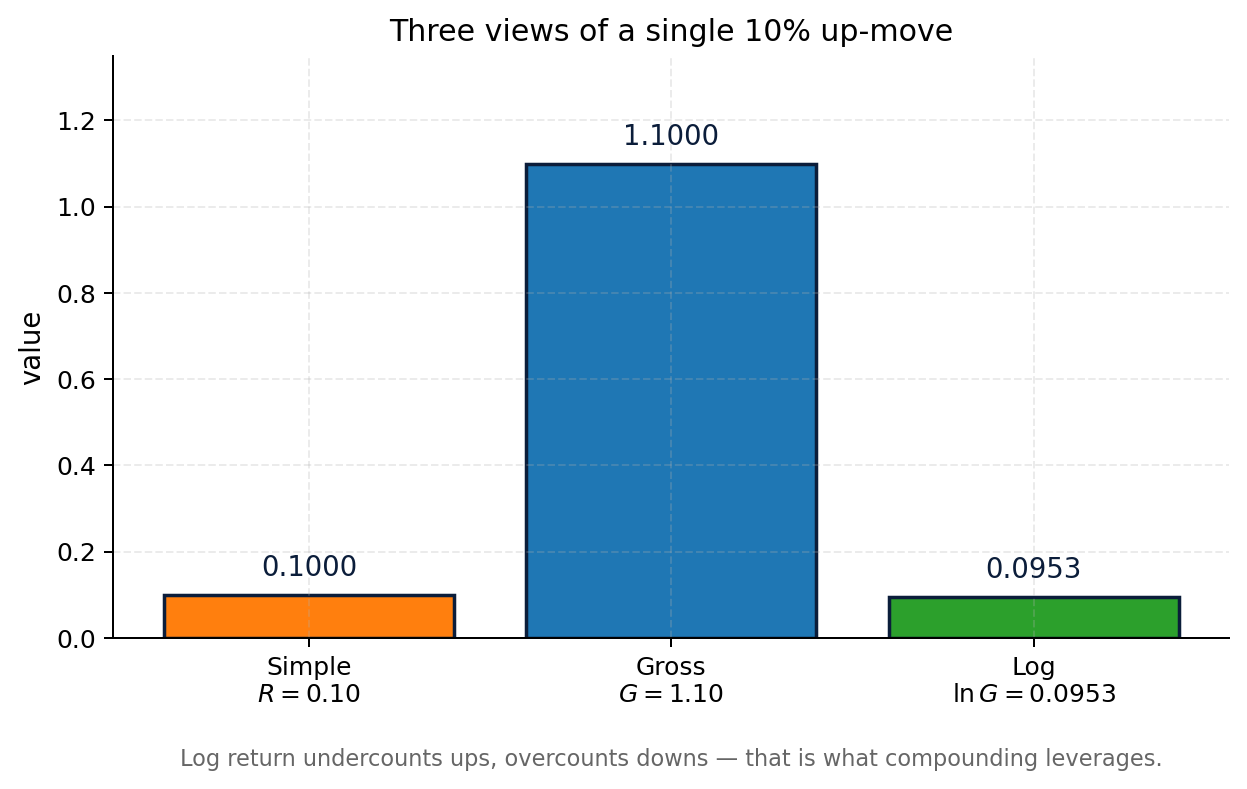
\includegraphics[keepaspectratio]{figures/ch00-gross-vs-log.png}}
\caption{Three views of a 10\% up-move: simple return \(R=0.10\), gross
return \(G=1.10\), log return \(\ln G=0.09531\). The log return
undercounts up-moves and overcounts down-moves; the gap is what
compounding will leverage over many periods.}
\end{figure}

\begin{figure}
\centering
\pandocbounded{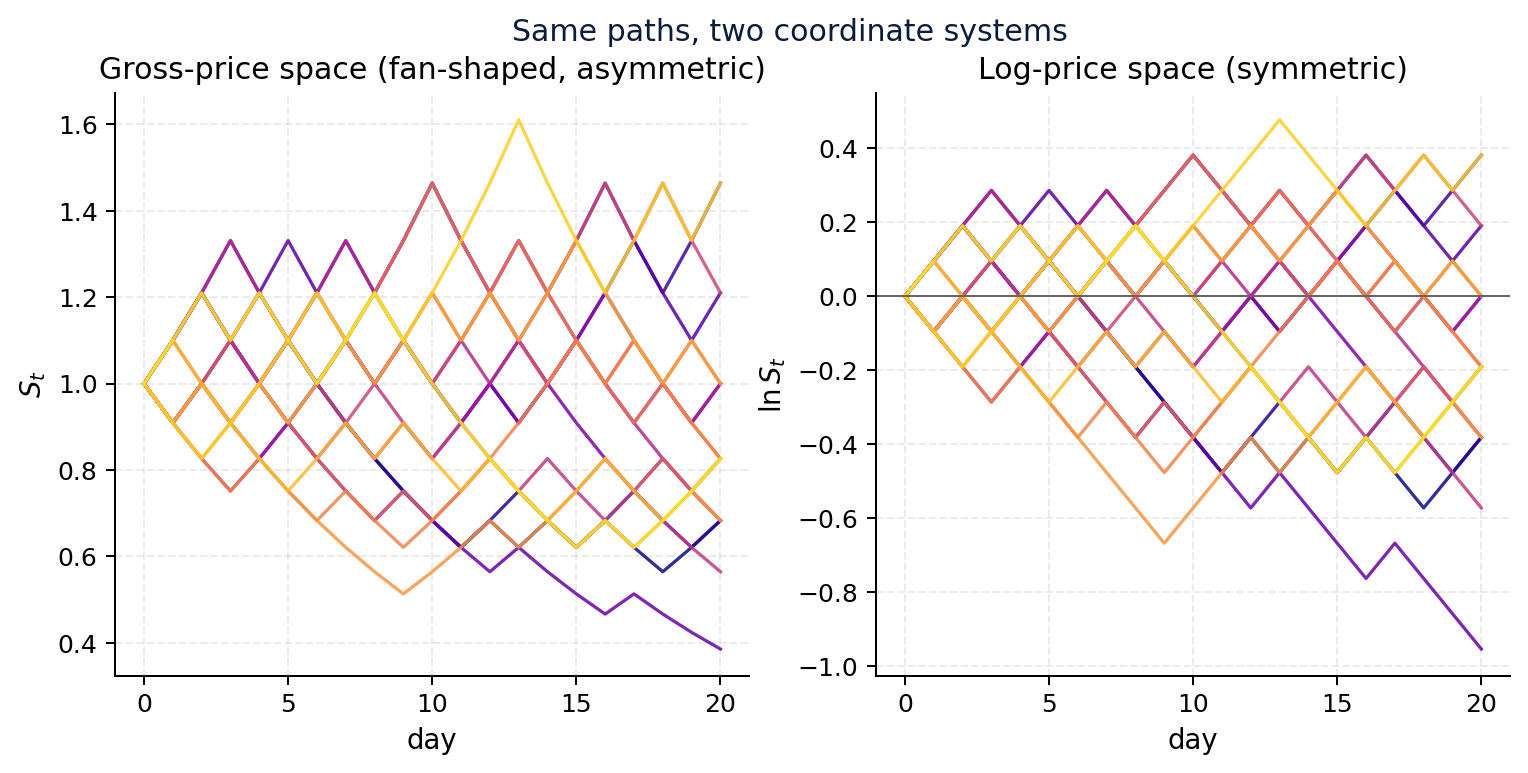
\includegraphics[keepaspectratio]{figures/ch00-paths-gross-vs-log.png}}
\caption{Twenty random binomial paths over 20 days plotted in
gross-price space (left, fan-shaped, asymmetric) and log-price space
(right, symmetric around the mean). The same paths look symmetric in log
coordinates because that is the additive coordinate of compounding.}
\end{figure}

\subsection{0.1.3 Table}\label{table}

\textbf{Table 0.1.} Gross-to-log conversion across a range of moves.

{\def\LTcaptype{none} % do not increment counter
\begin{table}[H]
\centering
\begin{tabular}{|r|r|r|r|}
\toprule
\(R\) & \(G = 1+R\) & \(\ln G\) & \(R - \ln G\) \\
\midrule



\(-0.50\) & \(0.50\) & \(-0.6931\) & \(+0.1931\) \\
\(-0.20\) & \(0.80\) & \(-0.2231\) & \(+0.0231\) \\
\(-0.10\) & \(0.90\) & \(-0.1054\) & \(+0.0054\) \\
\(-0.05\) & \(0.95\) & \(-0.0513\) & \(+0.0013\) \\
\(\phantom{+}0.00\) & \(1.00\) & \(\phantom{+}0.0000\) &
\(\phantom{+}0.0000\) \\
\(+0.05\) & \(1.05\) & \(\phantom{+}0.0488\) & \(+0.0012\) \\
\(+0.10\) & \(1.10\) & \(\phantom{+}0.0953\) & \(+0.0047\) \\
\(+0.20\) & \(1.20\) & \(\phantom{+}0.1823\) & \(+0.0177\) \\
\(+0.50\) & \(1.50\) & \(\phantom{+}0.4055\) & \(+0.0945\) \\
\bottomrule
\end{tabular}
\end{table}
}

\subsection{0.1.4 Exercises}\label{exercises}

\begin{enumerate}
\def\labelenumi{\arabic{enumi}.}
\tightlist
\item
  Five gross returns \(1.02, 0.98, 1.05, 0.95, 1.01\). Total gross? Log
  sum? \textbf{Answer:} \(1.00777\), \(0.00774\).
\item
  Daily \(u = 1.05\), \(d = 0.95\); the path DUDU over 4 days. Final
  price ratio? \textbf{Answer:} \(0.99750\).
\item
  \(S_0 = 100\), \(S_4 = 121\). Average log return per period?
  \textbf{Answer:} \(\ln(1.21)/4 = 0.04766\).
\end{enumerate}

\begin{center}\rule{0.5\linewidth}{0.5pt}\end{center}

\section{§0.2 Exponentials, Logarithms, Continuous Compounding (No
Calculus)}\label{exponentials-logarithms-continuous-compounding-no-calculus}

\textbf{Punchline.} The function \(e^x\) is the partner of \(\ln x\):
\(\ln(e^x) = x\) and \(e^{\ln x} = x\). Continuous compounding is the
\emph{identity} \(\lim_{n\to\infty}(1 + r/n)^n = e^r\) --- stated as a
fact, not derived. It says: as you compound more and more often at total
rate \(r\), you converge to multiplying by \(e^r\).

\textbf{Intuition.} Imagine you have \$1 and earn 100\% per year.
Compounded once: \$2. Compounded twice (50\% then 50\% on a bigger
base): \(1.5 \times 1.5 = \$2.25\). Compounded daily: \(\$2.71\).
Compounded continuously: \(\$2.71828 = e\). The number \(e\) is just
\emph{the limit of ``compound as often as possible at total rate 1.''}
Every continuous-compounding formula in the book is shorthand for ``I
compounded a lot of times.''

\subsection{0.2.1 Rules to memorise}\label{rules-to-memorise}

Both functions are \emph{just functions} --- you can look them up in a
table, in a calculator, or in Python. The arithmetic rules are:

\[e^{a+b} = e^a e^b, \qquad (e^a)^b = e^{ab}, \qquad e^0 = 1.\]
\[\ln(ab) = \ln a + \ln b, \qquad \ln(a^b) = b \ln a, \qquad \ln 1 = 0, \qquad \ln e = 1.\]
\[\ln(e^x) = x, \qquad e^{\ln x} = x \quad (x > 0).\]

The \emph{continuous compounding identity}, stated as a fact:

\[\lim_{n \to \infty} \left(1 + \frac{r}{n}\right)^{n} \;=\; e^{r}, \qquad \lim_{n \to \infty} \left(1 + \frac{r}{n}\right)^{nT} \;=\; e^{rT}.\]

That is the only ``limit'' in the book that the reader needs to take on
faith. We never differentiate \(e^x\), we never take its calculus
derivative; we use it as a function with the algebraic rules above.

\subsection{0.2.2 Examples}\label{examples-1}

\textbf{Example 0.2.1 (compounding converges to \(e^r\)).} Take
\(r = 0.05\), \(T = 1\) year. The value of \$1 invested at \(5\%\) for
one year, compounded at different frequencies:

{\def\LTcaptype{none} % do not increment counter
\begin{table}[H]
\centering
\begin{tabular}{|l|l|r|}
\toprule
Compounding & Formula & Value of \$1 \\
\midrule



Annual & \(1.05\) & \(1.05000\) \\
Semi-annual & \((1 + 0.05/2)^2\) & \(1.05063\) \\
Quarterly & \((1 + 0.05/4)^4\) & \(1.05095\) \\
Monthly & \((1 + 0.05/12)^{12}\) & \(1.05116\) \\
Daily & \((1 + 0.05/252)^{252}\) & \(1.05127\) \\
Continuous & \(e^{0.05}\) & \(1.05127\) \\
\bottomrule
\end{tabular}
\end{table}
}

Daily and continuous already agree to five decimal places.

\textbf{Example 0.2.2 (Toy).} \(r = 0.25\) for one period. Annual gross:
\(1.25\). Continuous gross: \(e^{0.25} = 1.28403\). The gap (\$0.034 per
dollar) widens at higher rates because \(e^r\) grows faster than
\(1 + r\).

\textbf{Example 0.2.3 (present value).} PV of \$100 due in 2 years at
\(r = 4\%\) continuous:
\(100 \cdot e^{-0.08} = 100 \cdot 0.92312 = \$92.31\). The same \$100
discounted \emph{annually} at \(4\%\) would be
\(100 / 1.04^2 = \$92.46\). Continuous discounting pulls slightly
harder.

\textbf{Example 0.2.4 (solving for a rate).} A bond pays \$100 in 1 year
and trades at \$95. What is the continuous yield?
\(100 e^{-r} = 95 \Rightarrow e^{-r} = 0.95 \Rightarrow r = -\ln 0.95 = 0.05129 = 5.13\%\).

\textbf{Example 0.2.5 (doubling time).} At a continuous rate \(r\), the
time to double is \(T = \ln 2 / r\). At \(r = 7\%\):
\(T = 0.6931 / 0.07 = 9.90\) years. (This is the rule of 72 with
\(72/7 = 10.3\) years; the rule of 72 is the simple-interest
approximation of \(\ln 2 / r\).)

\textbf{Example 0.2.6 (compounding identity by hand).} Compute
\((1 + 0.10/4)^{12}\). Step 1: \(1 + 0.025 = 1.025\). Step 2:
\(1.025^2 = 1.0506\). Step 3: \(1.025^4 = 1.0506^2 = 1.1038\). Step 4:
\(1.025^{12} = (1.025^4)^3 = 1.1038^3 = 1.3449\). That's the value of
\$1 quarterly-compounded at \(10\%\) for 3 years. Continuous comparison:
\(e^{0.30} = 1.3499\). About 0.4\% lower.

\begin{figure}
\centering
\pandocbounded{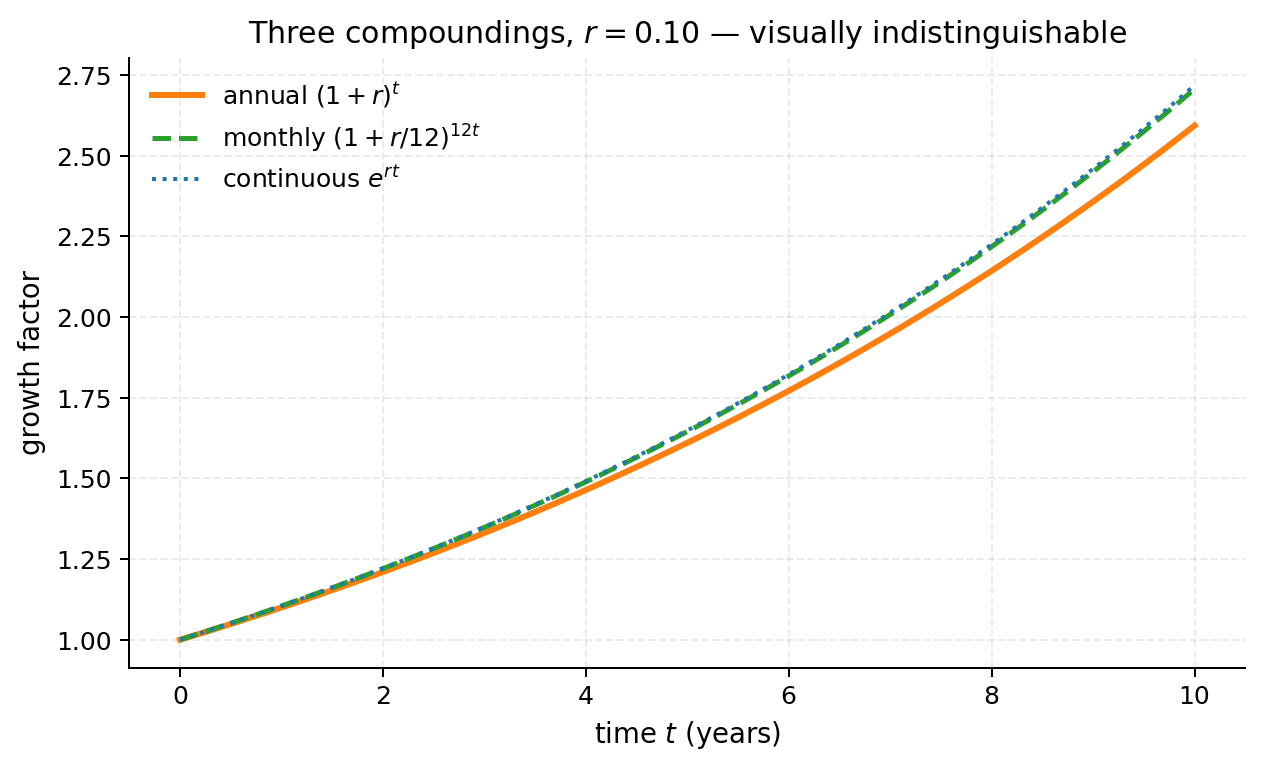
\includegraphics[keepaspectratio]{figures/ch00-compounding-converges.png}}
\caption{Three compounding curves for \(r=0.10\) as a function of time
\(t\): annual \((1.1)^t\), monthly \((1+0.10/12)^{12t}\), and continuous
\(e^{0.10t}\). The three are visually indistinguishable beyond a few
years --- continuous compounding is the convenient limit, not a
different beast.}
\end{figure}

\begin{figure}
\centering
\pandocbounded{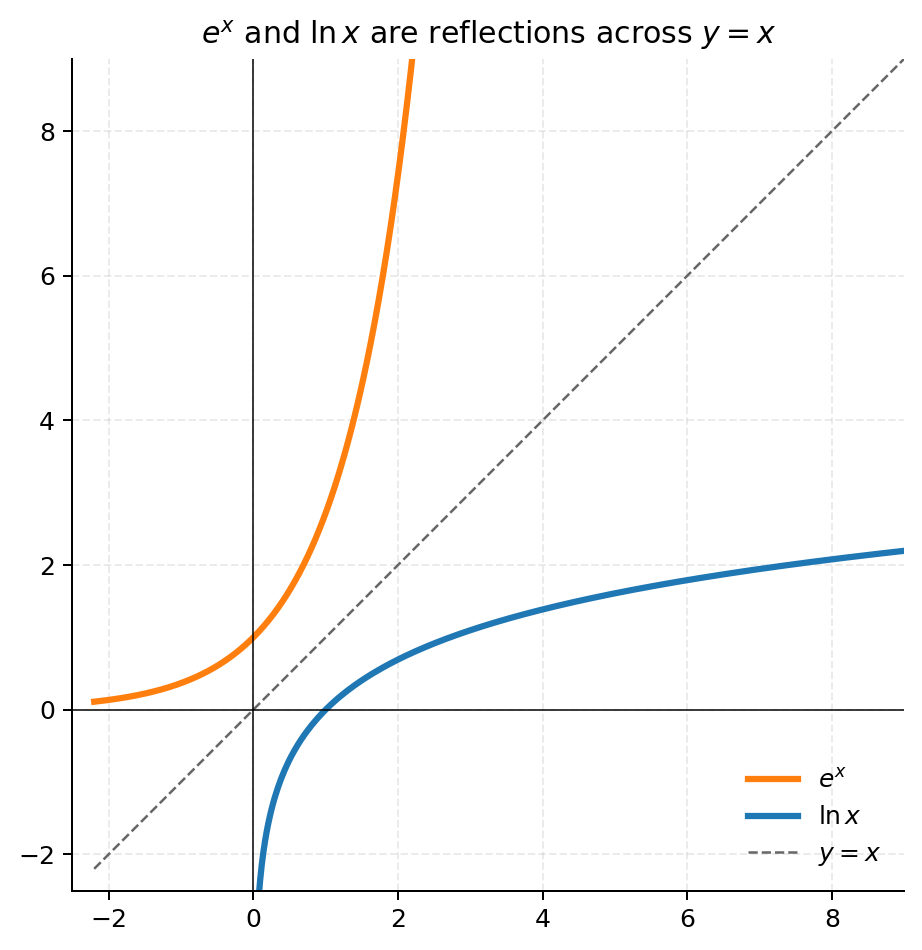
\includegraphics[keepaspectratio]{figures/ch00-exp-and-log.png}}
\caption{The exponential \(e^x\) and logarithm \(\ln x\) side by side,
reflections of one another across \(y=x\). The reader will use \(e^x\)
for compounding and \(\ln x\) for log returns; their reflection is the
visual statement of ``\(\ln\) undoes \(e\).''}
\end{figure}

\subsection{0.2.3 Tables}\label{tables}

\textbf{Table 0.2.} Compounding ladder: value of \$1 after 1 year at
three different rates, across compounding frequencies.

{\def\LTcaptype{none} % do not increment counter
\begin{table}[H]
\centering
\begin{tabular}{|l|r|r|r|}
\toprule
Frequency & \(r = 5\%\) & \(r = 10\%\) & \(r = 25\%\) \\
\midrule



Annual & \(1.05000\) & \(1.10000\) & \(1.25000\) \\
Semi-annual & \(1.05063\) & \(1.10250\) & \(1.26563\) \\
Quarterly & \(1.05095\) & \(1.10381\) & \(1.27443\) \\
Monthly & \(1.05116\) & \(1.10471\) & \(1.28073\) \\
Daily & \(1.05127\) & \(1.10516\) & \(1.28392\) \\
\textbf{Continuous (\(e^r\))} & \(\mathbf{1.05127}\) &
\(\mathbf{1.10517}\) & \(\mathbf{1.28403}\) \\
\bottomrule
\end{tabular}
\end{table}
}

\textbf{Table 0.3.} Common values of \(e^x\) and \(\ln x\).

{\def\LTcaptype{none} % do not increment counter
\begin{table}[H]
\centering
\begin{tabular}{|r|r|r|}
\toprule
\(x\) & \(e^x\) & \(\ln x\) \\
\midrule



\(0.01\) & \(\phantom{0}1.01005\) & \(-4.6052\) \\
\(0.05\) & \(\phantom{0}1.05127\) & \(-2.9957\) \\
\(0.10\) & \(\phantom{0}1.10517\) & \(-2.3026\) \\
\(0.25\) & \(\phantom{0}1.28403\) & \(-1.3863\) \\
\(0.50\) & \(\phantom{0}1.64872\) & \(-0.6931\) \\
\(1.00\) & \(\phantom{0}2.71828\) & \(\phantom{-}0.0000\) \\
\(2.00\) & \(\phantom{0}7.38906\) & \(\phantom{-}0.6931\) \\
\(3.00\) & \(20.08554\) & \(\phantom{-}1.0986\) \\
\bottomrule
\end{tabular}
\end{table}
}

\subsection{0.2.4 Exercises}\label{exercises-1}

\begin{enumerate}
\def\labelenumi{\arabic{enumi}.}
\tightlist
\item
  PV of \$250 in 3 years at \(r = 6\%\) continuous. \textbf{Answer:}
  \(250 e^{-0.18} = \$208.82\).
\item
  Solve \(\ln x = 2.5\). \textbf{Answer:} \(x = e^{2.5} = 12.182\).
\item
  Compare \((1 + 0.02/4)^{4 \cdot 5}\) with \(e^{0.02 \cdot 5}\).
  \textbf{Answer:} \(1.10494\) vs \(1.10517\) --- within \(0.02\%\).
\end{enumerate}

\begin{center}\rule{0.5\linewidth}{0.5pt}\end{center}

\section{§0.3 Sums, Products, Binomial Coefficients, Pascal, Binomial
Theorem}\label{sums-products-binomial-coefficients-pascal-binomial-theorem}

\textbf{Punchline.} The binomial coefficient
\(\binom{n}{k} = \dfrac{n!}{k!(n-k)!}\) counts paths. Pascal's triangle
\emph{is} the binomial tree with the stock price replaced by a count.
Every multi-period binomial pricing formula in Chapter 7 is a sum of the
form
\(\sum_k \binom{n}{k} \tilde p^k (1-\tilde p)^{n-k} (\text{payoff at } k)\).

\textbf{Intuition.} Imagine \(n\) coin flips. To end with exactly \(k\)
heads, you pick \emph{which} \(k\) of the \(n\) flips were heads ---
there are \(\binom{n}{k}\) ways to do that. If each particular sequence
has probability \(\tilde p^k (1-\tilde p)^{n-k}\), the total probability
of ``ended at \(k\) heads'' is the count times the per-sequence
probability. Pascal's recursion
\(\binom{n}{k} = \binom{n-1}{k-1} + \binom{n-1}{k}\) is just
\emph{``either the last flip was H (so we needed \(k-1\) heads before)
or it was T (so we needed \(k\) already).''}

\subsection{0.3.1 Definitions and
identities}\label{definitions-and-identities}

The \textbf{factorial} \(n! = 1 \cdot 2 \cdot 3 \cdots n\), with
\(0! = 1\) by convention.

The \textbf{binomial coefficient}:

\[\binom{n}{k} \;=\; \frac{n!}{k!\,(n-k)!} \qquad \text{for integers } 0 \le k \le n.\]

It reads ``\(n\) choose \(k\)'' --- the number of ways to choose \(k\)
objects from \(n\) without regard to order.

\textbf{Symmetry}: \(\binom{n}{k} = \binom{n}{n-k}\). (Choosing which
\(k\) are heads is the same as choosing which \(n-k\) are tails.)

\textbf{Pascal's recursion}:
\(\binom{n}{k} = \binom{n-1}{k-1} + \binom{n-1}{k}\). (Each entry is the
sum of the two above it.)

\textbf{Binomial theorem}:

\[(a + b)^n \;=\; \sum_{k=0}^{n} \binom{n}{k}\, a^k\, b^{n-k}.\]

Setting \(a = b = 1\): \(\sum_{k=0}^{n} \binom{n}{k} = 2^n\) --- the
rows of Pascal's triangle sum to powers of 2.

\subsection{0.3.2 Examples}\label{examples-2}

\textbf{Example 0.3.1 (small case enumerated).}
\(\binom{5}{2} = \dfrac{5!}{2! \cdot 3!} = \dfrac{120}{2 \cdot 6} = 10\).
Enumerate the 10 binary strings with exactly two heads:

\[\{\text{HHTTT, HTHTT, HTTHT, HTTTH, THHTT, THTHT, THTTH, TTHHT, TTHTH, TTTHH}\}.\]

\textbf{Example 0.3.2 (Pascal's triangle, rows 0--6).}

{\def\LTcaptype{none} % do not increment counter
\begin{table}[H]
\centering
\begin{tabular}{|l|l|r|}
\toprule
Row & Entries & Sum \\
\midrule



\(n=0\) & \(1\) & \(1\) \\
\(n=1\) & \(1\quad 1\) & \(2\) \\
\(n=2\) & \(1\quad 2\quad 1\) & \(4\) \\
\(n=3\) & \(1\quad 3\quad 3\quad 1\) & \(8\) \\
\(n=4\) & \(1\quad 4\quad 6\quad 4\quad 1\) & \(16\) \\
\(n=5\) & \(1\quad 5\quad 10\quad 10\quad 5\quad 1\) & \(32\) \\
\(n=6\) & \(1\quad 6\quad 15\quad 20\quad 15\quad 6\quad 1\) & \(64\) \\
\bottomrule
\end{tabular}
\end{table}
}

\textbf{Example 0.3.3 (binomial theorem with numbers).} Take
\(a = u = 1.10\), \(b = d = 0.90\), \(n = 4\). The binomial theorem
gives

\[(1.10 + 0.90)^4 \;=\; 2.00^4 \;=\; 16.0\]

decomposed as

\[\binom{4}{0}(0.90)^4 + \binom{4}{1}(1.10)(0.90)^3 + \binom{4}{2}(1.10)^2(0.90)^2 + \binom{4}{3}(1.10)^3(0.90) + \binom{4}{4}(1.10)^4.\]

Numerically:
\(0.6561 + 4 \cdot 0.8019 + 6 \cdot 0.9801 + 4 \cdot 1.1979 + 1.4641 = 0.6561 + 3.2076 + 5.8806 + 4.7916 + 1.4641 = 16.0000\).
✓

\textbf{Example 0.3.4 (paths in a binomial tree).} A 7-period binomial
tree has \(2^7 = 128\) paths. How many end at level \(+3\) (i.e., 5 ups
and 2 downs)?

\[\binom{7}{5} = \binom{7}{2} = \frac{7 \cdot 6}{2} = 21.\]

\textbf{Example 0.3.5 (Toy, \(n = 3\)).} \(S_0 = 4\), \(u = 2\),
\(d = 1/2\). The terminal nodes of a 3-period tree are

Each terminal price is \(S_3 = 4 \cdot u^k d^{3-k}\).

{\def\LTcaptype{none} % do not increment counter
\begin{table}[H]
\centering
\begin{tabular}{|c|c|c|}
\toprule
\(k\) & \(S_3\) & Paths \\
\midrule



\(0\) & \(1/2\) & \(1\) \\
\(1\) & \(2\) & \(3\) \\
\(2\) & \(8\) & \(3\) \\
\(3\) & \(32\) & \(1\) \\
\bottomrule
\end{tabular}
\end{table}
}

Total paths: \(1 + 3 + 3 + 1 = 8 = 2^3\). ✓

\textbf{Example 0.3.6 (realistic, \(n = 4\)).} \(S_0 = 100\),
\(u = 1.10\), \(d = 0.90\). Each terminal price is
\(S_4 = 100 \cdot u^k d^{4-k}\).

{\def\LTcaptype{none} % do not increment counter
\begin{table}[H]
\centering
\begin{tabular}{|c|r|c|}
\toprule
\(k\) & \(S_4\) & Paths \\
\midrule



\(0\) & \(65.61\) & \(1\) \\
\(1\) & \(80.19\) & \(4\) \\
\(2\) & \(98.01\) & \(6\) \\
\(3\) & \(119.79\) & \(4\) \\
\(4\) & \(146.41\) & \(1\) \\
\bottomrule
\end{tabular}
\end{table}
}

\textbf{Example 0.3.7 (Pascal recurrence in action).} Use Pascal's
recursion to compute \(\binom{10}{4}\) starting from row 9. From row 9:
\(\binom{9}{3} = 84\), \(\binom{9}{4} = 126\). So
\(\binom{10}{4} = 84 + 126 = 210\). Sanity check:
\(\binom{10}{4} = \dfrac{10 \cdot 9 \cdot 8 \cdot 7}{4!} = \dfrac{5040}{24} = 210\).
✓

\begin{figure}
\centering
\pandocbounded{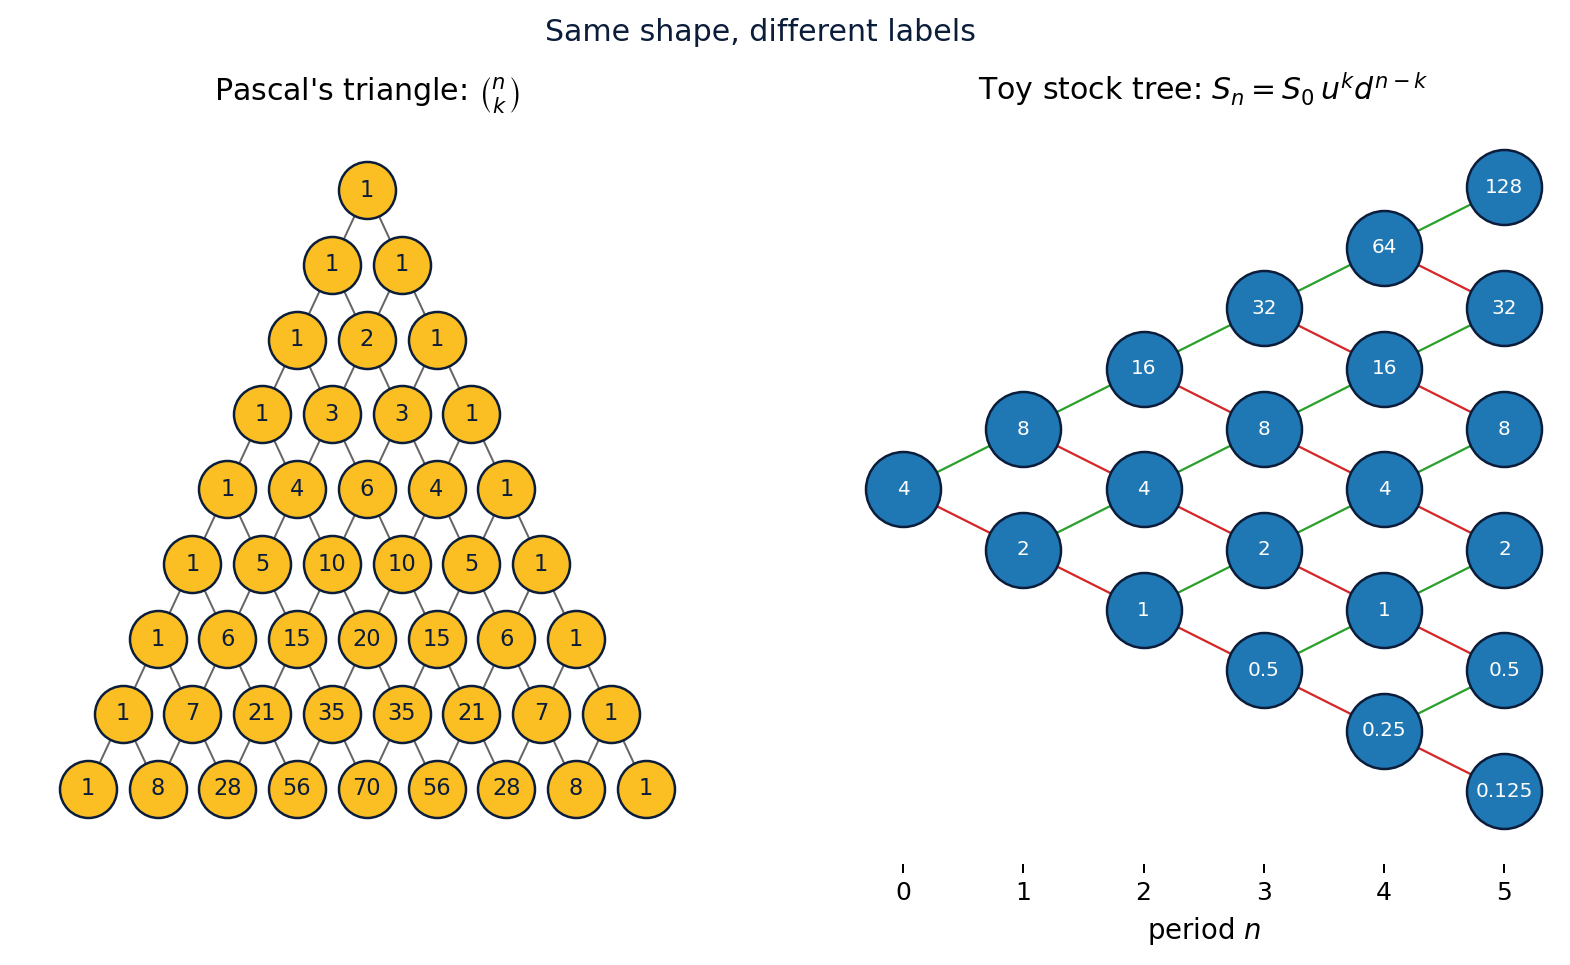
\includegraphics[keepaspectratio]{figures/ch00-pascal-vs-tree.png}}
\caption{Pascal's triangle through row 8, side-by-side with a binomial
stock tree (Toy: \(S_0=4, u=2, d=1/2\)). Same shape, different labels
--- left has path counts \(\binom{n}{k}\); right has the price
\(S_n = S_0 u^k d^{n-k}\).}
\end{figure}

\begin{figure}
\centering
\pandocbounded{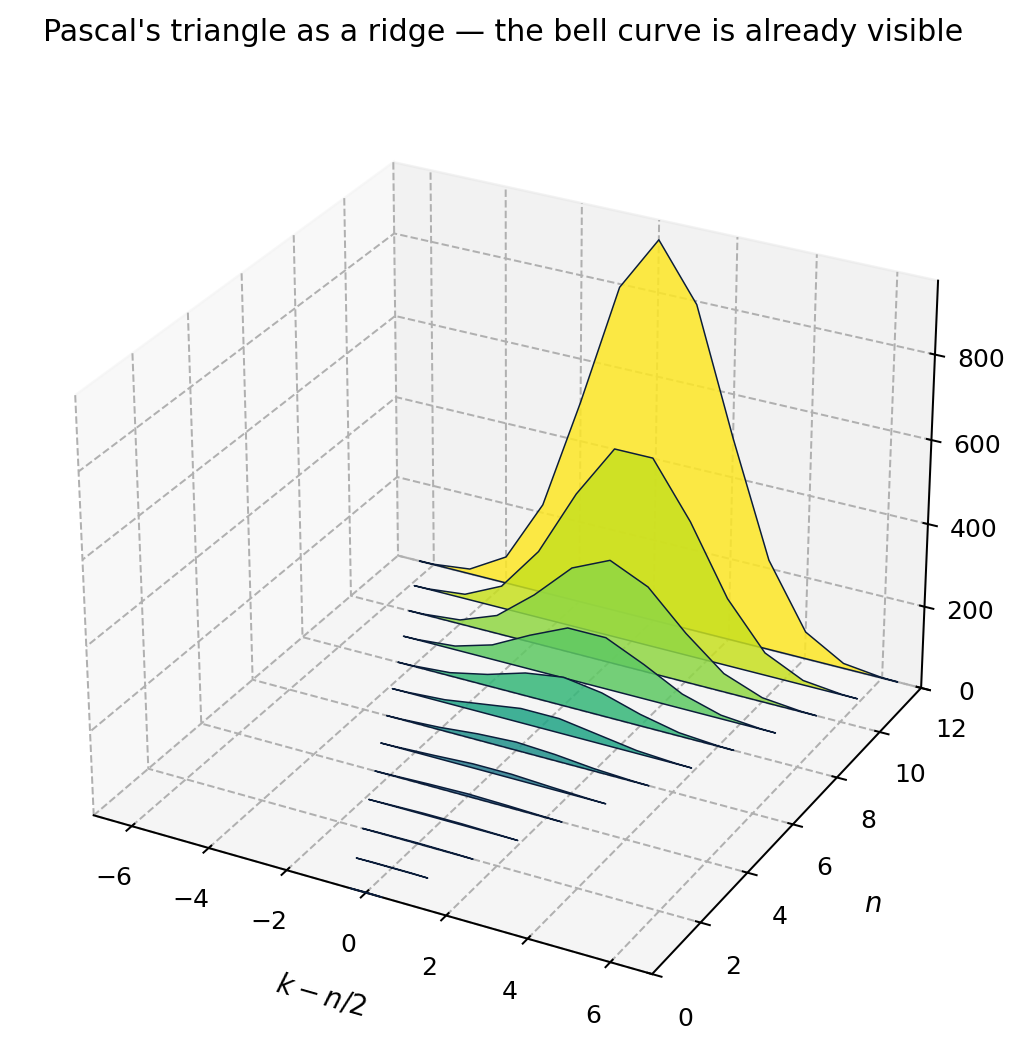
\includegraphics[keepaspectratio]{figures/ch00-pascal-3d.png}}
\caption{3-D bar chart of \(\binom{n}{k}\) for \(n = 0, 1, \dots, 12\).
Each row of Pascal's triangle plotted as bars; the central ridge
sharpens with \(n\), foreshadowing the bell curve that will emerge from
the Central Limit Theorem in §0.10.}
\end{figure}

\subsection{0.3.3 Table}\label{table-1}

\textbf{Table 0.4.} Terminal-node summary for the realistic 5-period
binomial tree, \(S_0 = 100\), \(u = 1.10\), \(d = 0.90\).

{\def\LTcaptype{none} % do not increment counter
\begin{table}[H]
\centering
\begin{tabular}{|r|r|r|r|}
\toprule
\(k\) & \(S_5 = 100\,u^k d^{5-k}\) & \(\binom{5}{k}\) &
\(\binom{5}{k}/2^5\) \\
\midrule



\(0\) & \(\phantom{0}59.05\) & \(\phantom{0}1\) & \(0.03125\) \\
\(1\) & \(\phantom{0}72.17\) & \(\phantom{0}5\) & \(0.15625\) \\
\(2\) & \(\phantom{0}88.21\) & \(10\) & \(0.31250\) \\
\(3\) & \(107.81\) & \(10\) & \(0.31250\) \\
\(4\) & \(131.77\) & \(\phantom{0}5\) & \(0.15625\) \\
\(5\) & \(161.05\) & \(\phantom{0}1\) & \(0.03125\) \\
\bottomrule
\end{tabular}
\end{table}
}

\subsection{0.3.4 Exercises}\label{exercises-2}

\begin{enumerate}
\def\labelenumi{\arabic{enumi}.}
\tightlist
\item
  Compute \(\binom{8}{3}\). \textbf{Answer:} \(56\).
\item
  Paths in a 10-step tree ending at level \(+4\). \textbf{Answer:}
  \(\binom{10}{7} = 120\).
\item
  Sum of row 8 of Pascal. \textbf{Answer:} \(2^8 = 256\).
\end{enumerate}

\begin{center}\rule{0.5\linewidth}{0.5pt}\end{center}

\section{§0.4 Probability on Finite Sample
Spaces}\label{probability-on-finite-sample-spaces}

\textbf{Punchline.} A probability is a weight on each leaf of a finite
tree. \emph{Events} are sets of leaves. The probability of an event is
the sum of its leaf weights. Conditional probability is \emph{``zoom
into a subtree and renormalise so the new weights sum to 1.''}
Everything Chapter 1 and Chapter 3 will say about risk-neutral
probability is built on this picture.

\textbf{Intuition.} Imagine tossing three coins. The sample space
\(\Omega\) is the set of 8 possible outcomes (HHH, HHT,\ldots, TTT). If
the coin is fair, each has weight \(1/8\). The event ``exactly two
heads'' is the set \(\{\)HHT, HTH, THH\(\}\) --- three leaves, total
weight \(3/8\). Conditioning on ``first toss is H'' zooms into the four
leaves starting with H; each had weight \(1/8\), now they renormalise to
\(1/4\) each.

\subsection{0.4.1 Definitions}\label{definitions-1}

A \textbf{sample space} \(\Omega\) is the finite set of all possible
outcomes of a random experiment.

An \textbf{event} \(A\) is a subset \(A \subseteq \Omega\).

A \textbf{probability measure} \(\mathbb{P}\) assigns a weight
\(p(\omega) \geq 0\) to every \(\omega \in \Omega\), such that
\(\sum_{\omega \in \Omega} p(\omega) = 1\). The probability of any event
\(A\) is

\[\mathbb{P}(A) \;=\; \sum_{\omega \in A} p(\omega).\]

For two events \(A, B\):

\[\mathbb{P}(A \cup B) \;=\; \mathbb{P}(A) + \mathbb{P}(B) - \mathbb{P}(A \cap B), \qquad \mathbb{P}(A^c) \;=\; 1 - \mathbb{P}(A).\]

\textbf{Conditional probability}:

\[\mathbb{P}(A \mid B) \;=\; \frac{\mathbb{P}(A \cap B)}{\mathbb{P}(B)}, \qquad \text{provided } \mathbb{P}(B) > 0.\]

Two events are \textbf{independent} if
\(\mathbb{P}(A \cap B) = \mathbb{P}(A)\,\mathbb{P}(B)\), equivalently
\(\mathbb{P}(A \mid B) = \mathbb{P}(A)\).

\textbf{Bayes' rule} (just rearranging the definition):

\[\mathbb{P}(A \mid B) \;=\; \frac{\mathbb{P}(B \mid A)\,\mathbb{P}(A)}{\mathbb{P}(B)}.\]

\subsection{0.4.2 Examples}\label{examples-3}

\textbf{Example 0.4.1 (two fair coins).} \(\Omega = \{\)HH, HT, TH,
TT\(\}\), each leaf weight \(1/4\). The event ``both heads'' is the
singleton \(\{\)HH\(\}\), probability \(1/4\).

\textbf{Example 0.4.2 (exactly one head).} The event is \(\{\)HT,
TH\(\}\), probability \(2/4 = 1/2\).

\textbf{Example 0.4.3 (biased three-toss).} \(p = 0.6\) for heads.
Compute \(\mathbb{P}(\)HHT\() = 0.6 \cdot 0.6 \cdot 0.4 = 0.144\). The
sample space has 8 leaves; their weights are

{\def\LTcaptype{none} % do not increment counter
\begin{table}[H]
\centering
\begin{tabular}{|l|r|}
\toprule
Outcome & Weight \\
\midrule



HHH & \(0.216\) \\
HHT & \(0.144\) \\
HTH & \(0.144\) \\
HTT & \(0.096\) \\
THH & \(0.144\) \\
THT & \(0.096\) \\
TTH & \(0.096\) \\
TTT & \(0.064\) \\
\bottomrule
\end{tabular}
\end{table}
}

(Total \(= 1\), as required.)

\textbf{Example 0.4.4 (conditional in a tree).} Two fair tosses. Given
that there is at least one head, what is the probability that both are
heads?

\[\mathbb{P}(\text{both H} \mid \geq 1 \text{ H}) = \frac{\mathbb{P}(\text{both H})}{\mathbb{P}(\geq 1\text{ H})} = \frac{1/4}{3/4} = \frac{1}{3}.\]

\textbf{Example 0.4.5 (independence check).} Two fair coins. Let \$A =
\{\(1st is H\)\}\$, \$B = \{\(2nd is H\)\}\$. Then
\(\mathbb{P}(A) = \mathbb{P}(B) = 1/2\) and
\(\mathbb{P}(A \cap B) = \mathbb{P}(\)HH\() = 1/4 = (1/2)(1/2)\). So
\(A \perp B\). ✓

\textbf{Example 0.4.6 (Bayes, the classic medical test).} A disease has
prevalence \(\mathbb{P}(\text{sick}) = 0.01\). A test has sensitivity
\(\mathbb{P}(+ \mid \text{sick}) = 0.99\) and specificity
\(\mathbb{P}(- \mid \text{healthy}) = 0.95\). You test positive --- what
is the probability you are sick?

\[
\mathbb{P}(\text{sick} \mid +)
\;=\; \frac{\mathbb{P}(+ \mid \text{sick})\,\mathbb{P}(\text{sick})}{\mathbb{P}(+ \mid \text{sick})\,\mathbb{P}(\text{sick}) + \mathbb{P}(+ \mid \text{healthy})\,\mathbb{P}(\text{healthy})}
\]

\[= \frac{0.99 \cdot 0.01}{0.99 \cdot 0.01 + 0.05 \cdot 0.99} = \frac{0.0099}{0.0099 + 0.0495} = \frac{0.0099}{0.0594} = 0.1667.\]

Only \(1\) in \(6\) positive tests are actually sick --- the famous
\emph{base-rate fallacy}. The same arithmetic underlies updating a prior
in Bayesian inference and is the engine of risk-neutral pricing's
``change of measure'' later in this book.

\textbf{Example 0.4.7 (at-least probability).} Three tosses,
\(p = 0.5\). Probability of at least one head?

\[\mathbb{P}(\geq 1 \text{ H}) = 1 - \mathbb{P}(0 \text{ H}) = 1 - 0.5^3 = 0.875.\]

The complement trick: directly summing the cases ``exactly 1, 2, or 3
heads'' is more work.

\begin{figure}
\centering
\pandocbounded{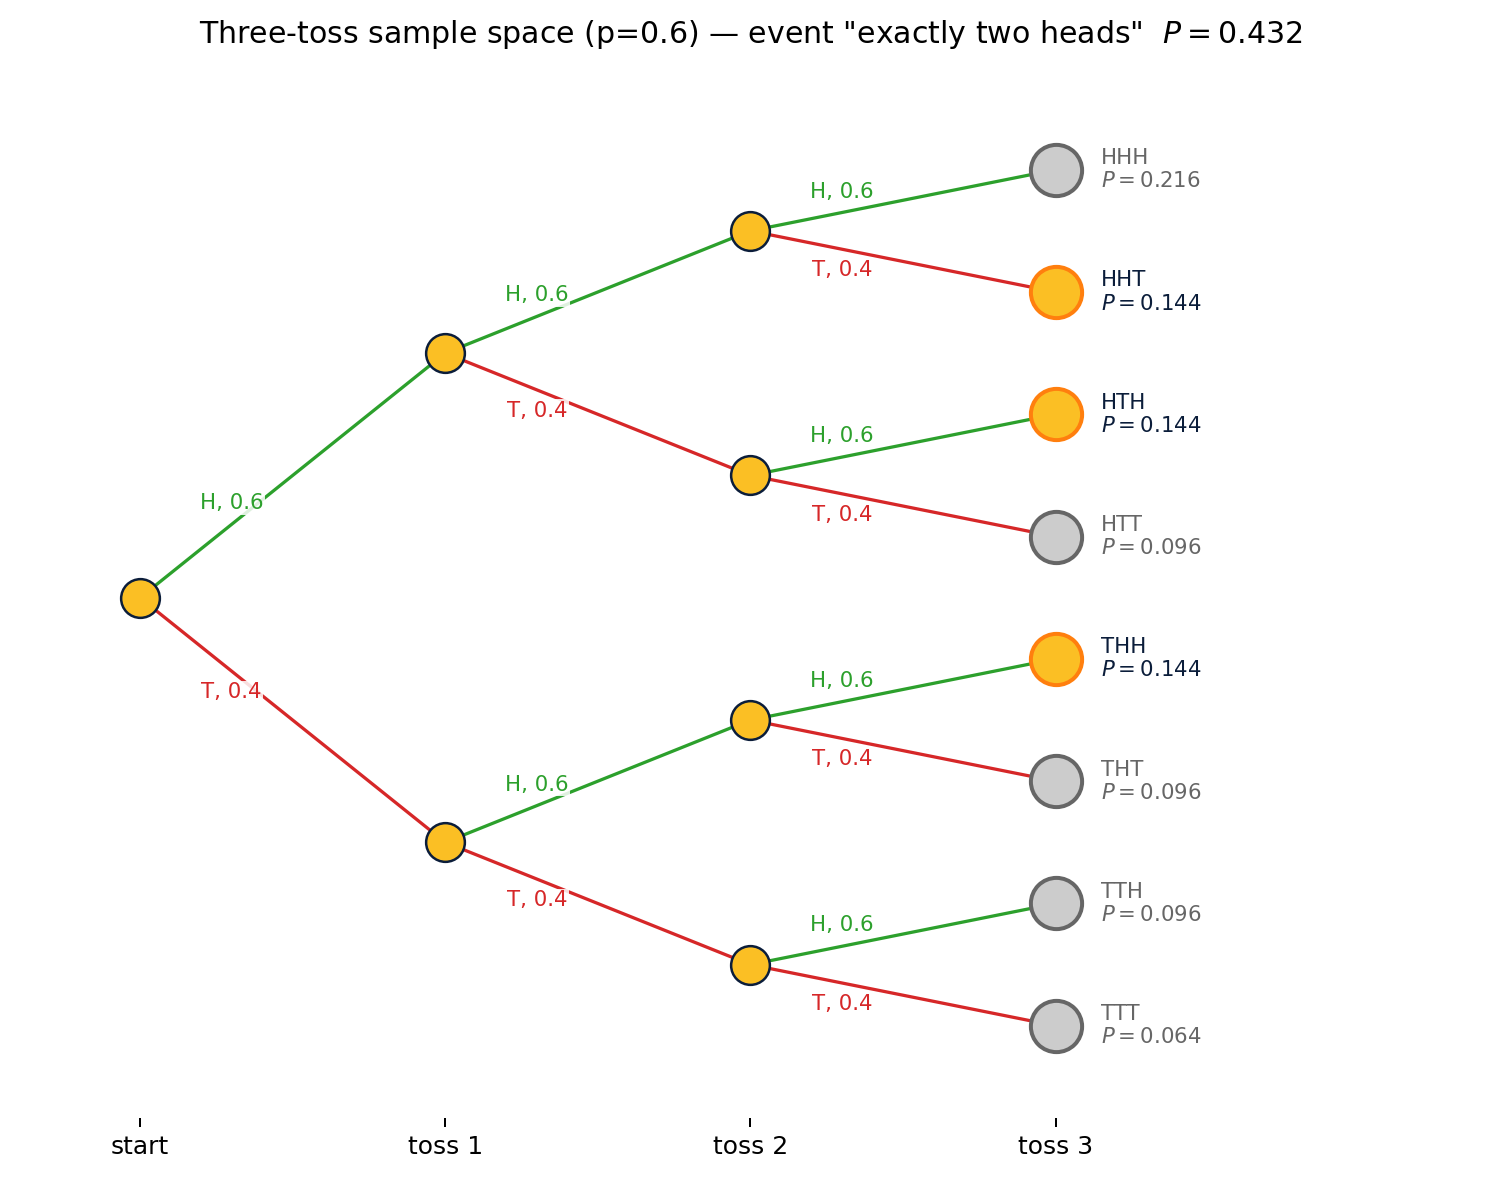
\includegraphics[keepaspectratio]{figures/ch00-sample-space-tree.png}}
\caption{Three-toss sample space drawn as an eight-leaf tree under
\(p = 0.6\). Each leaf is shaded according to whether it satisfies
``exactly two heads'' (the highlighted event). The probability is just
the sum of the highlighted weights.}
\end{figure}

\subsection{0.4.3 Tables}\label{tables-1}

\textbf{Table 0.5.} Joint distribution of two fair dice rolled,
summarised as (sum, max).

{\def\LTcaptype{none} % do not increment counter
\begin{table}[H]
\centering
\begin{tabular}{|l|r|r|r|r|r|r|r|}
\toprule
 & max \(=1\) & \(=2\) & \(=3\) & \(=4\) & \(=5\) & \(=6\) & sum-marg. \\
\midrule



sum \(=2\) & \(1/36\) & & & & & & \(1/36\) \\
\(=3\) & & \(2/36\) & & & & & \(2/36\) \\
\(=4\) & & \(1/36\) & \(2/36\) & & & & \(3/36\) \\
\(=5\) & & & \(2/36\) & \(2/36\) & & & \(4/36\) \\
\(=6\) & & & \(1/36\) & \(2/36\) & \(2/36\) & & \(5/36\) \\
\(=7\) & & & & \(2/36\) & \(2/36\) & \(2/36\) & \(6/36\) \\
\(=8\) & & & & \(1/36\) & \(2/36\) & \(2/36\) & \(5/36\) \\
\(=9\) & & & & & \(2/36\) & \(2/36\) & \(4/36\) \\
\(=10\) & & & & & \(1/36\) & \(2/36\) & \(3/36\) \\
\(=11\) & & & & & & \(2/36\) & \(2/36\) \\
\(=12\) & & & & & & \(1/36\) & \(1/36\) \\
max-marg. & \(1/36\) & \(3/36\) & \(5/36\) & \(7/36\) & \(9/36\) &
\(11/36\) & \(36/36\) \\
\bottomrule
\end{tabular}
\end{table}
}

\emph{Blank: \((sum, max)\) pair is impossible (e.g.~sum \(=3\) with
\(\max=1\) requires both dice \(\le 1\) but they must sum to \(3\)).}

\subsection{0.4.4 Exercises}\label{exercises-3}

\begin{enumerate}
\def\labelenumi{\arabic{enumi}.}
\tightlist
\item
  Three fair tosses, \(\mathbb{P}(\)exactly 2 heads\()\).
  \textbf{Answer:} \(3/8\).
\item
  Two dice, \(\mathbb{P}(\)sum \(= 7)\). \textbf{Answer:} \(1/6\).
\item
  Two dice, given sum \(= 7\): \(\mathbb{P}(\)first die was 3\()\).
  \textbf{Answer:} \(1/6\) (one of six equally-likely \((a, 7-a)\)
  pairs).
\end{enumerate}

\begin{center}\rule{0.5\linewidth}{0.5pt}\end{center}

\section{§0.5 Random Variables, Expectation,
Variance}\label{random-variables-expectation-variance}

\textbf{Punchline.} \(\mathbb{E}\) is linear \emph{always}.
\(\mathrm{Var}\) adds \emph{only} for independent things. These two
rules do most of the algebra in derivatives pricing.

\textbf{Intuition.} A random variable is a number assigned to each leaf
of the sample-space tree. The \emph{expectation} is the
leaf-weight-weighted average. The \emph{variance} measures how spread
out those leaf values are around the mean. Linearity says: averaging is
commutative with arithmetic --- if you double every payoff, the average
doubles. Independence of variance says: spread of a sum equals sum of
spreads, but \emph{only} when the two random variables don't share
information.

\subsection{0.5.1 Definitions}\label{definitions-2}

A \textbf{random variable} \(X\) is a function
\(X : \Omega \to \mathbb{R}\). (For discrete \(\Omega\) it just assigns
a number to each outcome.)

The \textbf{probability mass function (PMF)} lists the values \(X\)
takes and their probabilities:

\[\mathbb{P}(X = x) \;=\; \sum_{\omega : X(\omega) = x} p(\omega).\]

The \textbf{expectation}:

\[\mathbb{E}[X] \;=\; \sum_{\omega \in \Omega} X(\omega)\, p(\omega) \;=\; \sum_{x} x\, \mathbb{P}(X = x).\]

The \textbf{variance} and \textbf{standard deviation}:

\[\mathrm{Var}(X) \;=\; \mathbb{E}\!\left[(X - \mathbb{E}[X])^2\right] \;=\; \mathbb{E}[X^2] - (\mathbb{E}[X])^2, \qquad \sigma_X = \sqrt{\mathrm{Var}(X)}.\]

The \textbf{two rules} that govern almost every calculation:

\begin{itemize}
\tightlist
\item
  \textbf{Linearity} (always holds):
  \(\mathbb{E}[aX + bY + c] = a\,\mathbb{E}[X] + b\,\mathbb{E}[Y] + c\).
\item
  \textbf{Variance under scaling}:
  \(\mathrm{Var}(aX + c) = a^2\,\mathrm{Var}(X)\).
\item
  \textbf{Variance of independent sum}: if \(X \perp Y\), then
  \(\mathrm{Var}(X + Y) = \mathrm{Var}(X) + \mathrm{Var}(Y)\).
\end{itemize}

Independence does not show up in \(\mathbb{E}\)'s additivity (which
always holds); it shows up in \(\mathrm{Var}\)'s additivity.

\subsection{0.5.2 Examples}\label{examples-4}

\textbf{Example 0.5.1 (fair six-sided die).}
\(X \in \{1, 2, 3, 4, 5, 6\}\), each with probability \(1/6\).

\begin{itemize}
\tightlist
\item
  \(\mathbb{E}[X] = (1+2+3+4+5+6)/6 = 21/6 = 3.5\).
\item
  \(\mathbb{E}[X^2] = (1+4+9+16+25+36)/6 = 91/6 = 15.167\).
\item
  \(\mathrm{Var}(X) = 15.167 - 3.5^2 = 15.167 - 12.25 = 2.917\).
\item
  \(\sigma_X = \sqrt{2.917} = 1.708\).
\end{itemize}

\textbf{Example 0.5.2 (Bernoulli).} \(X\) is \(1\) with probability
\(p\), \(0\) with probability \(1-p\).

\begin{itemize}
\tightlist
\item
  \(\mathbb{E}[X] = p\).
\item
  \(\mathbb{E}[X^2] = p\) (since \(X^2 = X\)).
\item
  \(\mathrm{Var}(X) = p - p^2 = p(1-p)\).
\end{itemize}

At \(p = 0.6\): \(\mathbb{E} = 0.6\), \(\mathrm{Var} = 0.24\),
\(\sigma = 0.490\).

\textbf{Example 0.5.3 (Toy, one-period stock).} \(S_0 = 4\),
\(S_1 \in \{8, 2\}\), with risk-neutral probability \(\tilde p = 1/2\)
on each.

\begin{itemize}
\tightlist
\item
  \(\tilde{\mathbb{E}}[S_1] = (1/2)(8) + (1/2)(2) = 5\).
\item
  Discount at \(1/(1+r) = 1/(1 + 1/4) = 4/5\): \((4/5)(5) = 4 = S_0\). ✓
  The discounted expected price \emph{is} the current price under
  \(\tilde{\mathbb{P}}\). This is the seed of Chapter 1's risk-neutral
  pricing formula.
\end{itemize}

\textbf{Example 0.5.4 (realistic one-period stock).} \(S_0 = 100\),
\(S_1 \in \{110, 90\}\), real-world probability \(p = 0.6\).

\begin{itemize}
\tightlist
\item
  \(\mathbb{E}[S_1] = 0.6 \cdot 110 + 0.4 \cdot 90 = 66 + 36 = 102\).
\item
  \(\mathbb{E}[S_1^2] = 0.6 \cdot 12100 + 0.4 \cdot 8100 = 7260 + 3240 = 10500\).
\item
  \(\mathrm{Var}(S_1) = 10500 - 102^2 = 10500 - 10404 = 96\).
\item
  \(\sigma_{S_1} = \sqrt{96} = 9.80\).
\end{itemize}

So the price next period has expected value \$102 and SD \$9.80.

\textbf{Example 0.5.5 (sum of 100 iid Bernoulli(0.5)).} Let
\(H = X_1 + \dots + X_{100}\) where each \(X_i \sim\)
Bernoulli\((0.5)\).

\begin{itemize}
\tightlist
\item
  \(\mathbb{E}[H] = 100 \cdot 0.5 = 50\).
\item
  \(\mathrm{Var}(H) = 100 \cdot 0.5 \cdot 0.5 = 25\) (independent
  summands).
\item
  \(\sigma_H = 5\).
\end{itemize}

100 fair coin flips have mean 50 heads and SD 5; the \emph{fraction} of
heads has mean \(0.5\) and SD \(0.05\). We will reuse this in §0.10.

\textbf{Example 0.5.6 (sum of two dice).} Let \(X, Y\) be two
independent fair dice.

\begin{itemize}
\tightlist
\item
  \(\mathbb{E}[X + Y] = 3.5 + 3.5 = 7\).
\item
  \(\mathrm{Var}(X + Y) = 2.917 + 2.917 = 5.833\) (independent).
\end{itemize}

\textbf{Example 0.5.7 (variance under scaling --- a common trap).} \(X\)
is one fair die. \(\mathrm{Var}(X) = 2.917\). Now \(Y = 2X\) (e.g., a
die where every face is doubled). Then
\(\mathrm{Var}(Y) = 4 \cdot 2.917 = 11.67\). \emph{Not}
\(2 \cdot 2.917\). The factor squares because variance is ``average
squared deviation.''

\textbf{Example 0.5.8 (lottery expected value).} A ticket costs \$5 and
pays \$1\{,\}000\{,\}000 with probability \(10^{-7}\). Expected profit:

\[\mathbb{E}[\text{profit}] = 10^{-7} \cdot 1{,}000{,}000 - (1 - 10^{-7}) \cdot 5 \approx 0.10 - 5 = -\$4.90.\]

The ticket has expected loss \$4.90.

\begin{figure}
\centering
\pandocbounded{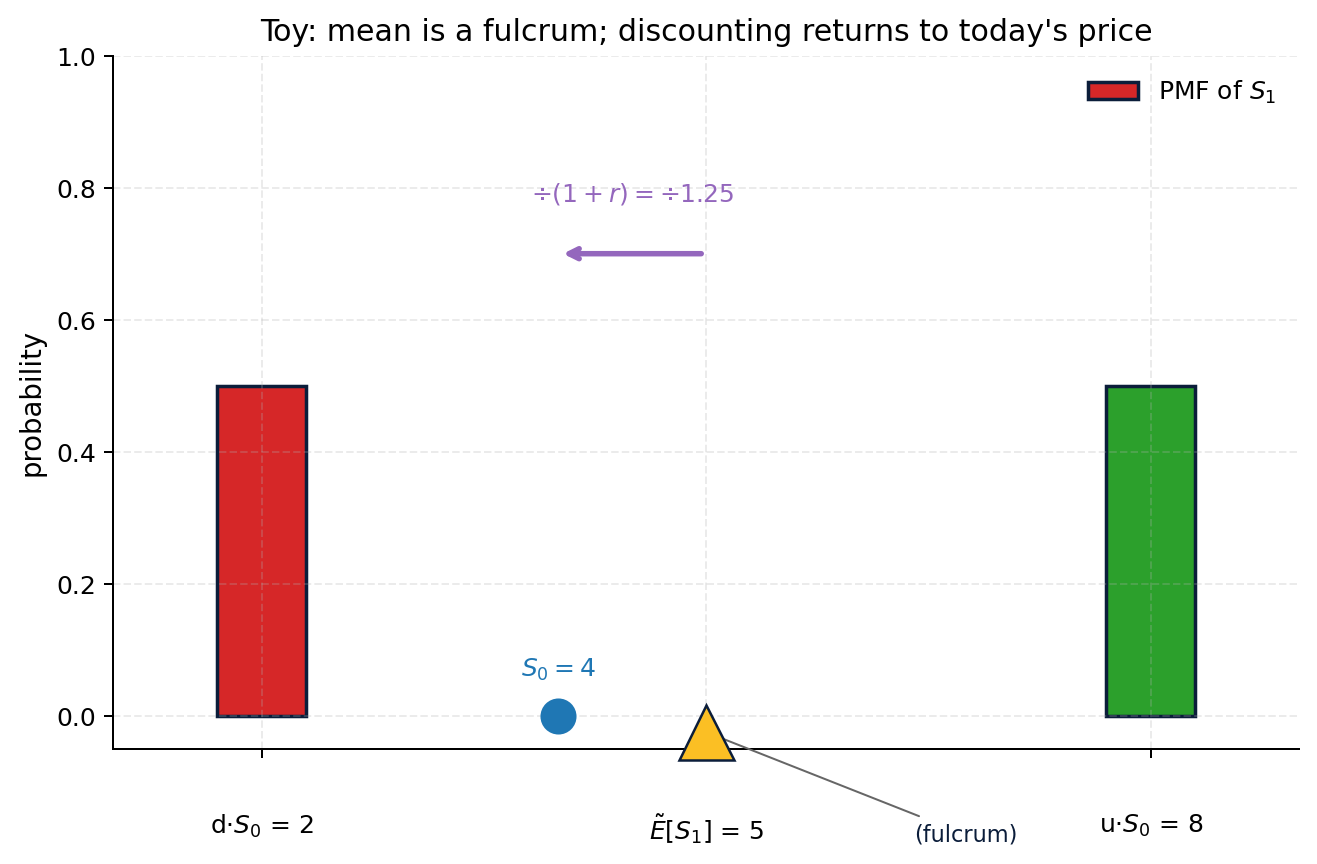
\includegraphics[keepaspectratio]{figures/ch00-mean-as-fulcrum.png}}
\caption{Two-state stock under Toy (\(S_0=4, u=2, d=1/2\),
\(\tilde p=1/2\)): the bar PMF of \(S_1\) with the mean marked as a
triangle, and the discount line
\((1+r)^{-1} \tilde{\mathbb{E}}[S_1] = S_0\) shown as an arrow. The mean
is a fulcrum; the discount factor moves it back to today's price.}
\end{figure}

\subsection{0.5.3 Table}\label{table-2}

\textbf{Table 0.6.} Bernoulli summary: mean and variance as \(p\)
varies.

{\def\LTcaptype{none} % do not increment counter
\begin{table}[H]
\centering
\begin{tabular}{|r|r|r|r|}
\toprule
\(p\) & \(\mathbb{E}[X]\) & \(\mathrm{Var}(X)\) & \(\sigma_X\) \\
\midrule



\(0.10\) & \(0.100\) & \(0.090\) & \(0.300\) \\
\(0.30\) & \(0.300\) & \(0.210\) & \(0.458\) \\
\(0.50\) & \(0.500\) & \(0.250\) & \(0.500\) \\
\(0.70\) & \(0.700\) & \(0.210\) & \(0.458\) \\
\(0.90\) & \(0.900\) & \(0.090\) & \(0.300\) \\
\bottomrule
\end{tabular}
\end{table}
}

The variance is maximised at \(p = 0.5\) --- the fairest coin is the
most uncertain.

\subsection{0.5.4 Exercises}\label{exercises-4}

\begin{enumerate}
\def\labelenumi{\arabic{enumi}.}
\tightlist
\item
  \(X\) uniform on \(\{1, 2, \dots, 10\}\). Mean? Variance?
  \textbf{Answer:} \(5.5\), \(8.25\).
\item
  Sum of 50 fair coin flips: variance. \textbf{Answer:}
  \(50 \cdot 0.25 = 12.5\).
\item
  \(u = 1.20\), \(d = 0.80\), \(p = 0.5\). \(\mathbb{E}[S_1/S_0]\) and
  \(\sigma\)? \textbf{Answer:} \(1.00\), \(0.20\).
\end{enumerate}

\begin{center}\rule{0.5\linewidth}{0.5pt}\end{center}

\section{§0.6 Conditional Expectation on
Trees}\label{conditional-expectation-on-trees}

\textbf{Punchline.} \(\mathbb{E}[X \mid \mathcal{F}_n]\) is \emph{the
best forecast of \(X\) given what you know at time \(n\)}. On a tree, it
is the probability-weighted average over the subtree rooted at the
current node. The \textbf{tower property} ---
\(\mathbb{E}[\mathbb{E}[X \mid \mathcal{F}_n]] = \mathbb{E}[X]\) --- is
just ``averaging in two stages gives the same answer as averaging in
one.''

\textbf{Intuition.} Imagine you are at a node halfway through a binomial
tree. You don't yet know whether the next toss will be H or T, but you
can list the remaining branches and their probabilities. The conditional
expectation at \emph{your} node is just the average of \(X\) over those
remaining branches, weighted by their conditional probabilities. The
tower property says: if a friend at a still-earlier node averages over
\emph{your} possible conditional expectations, they recover the original
full-tree average. \emph{Backward induction in Chapter 2 is exactly this
tower property applied step by step from the leaves to the root.}

\subsection{0.6.1 Definitions}\label{definitions-3}

The \textbf{information at time \(n\)}, written \(\mathcal{F}_n\), is a
partition of \(\Omega\) --- a list of disjoint ``blocks''
\(A_n(\omega)\) such that every \(\omega\) sits in exactly one block,
and within a block all outcomes are indistinguishable from the
time-\(n\) vantage. On a binomial tree, \(\mathcal{F}_n\) is the
partition by \emph{which node at level \(n\) the path currently sits
in}.

The \textbf{conditional expectation} of \(X\) given \(\mathcal{F}_n\) is
a \emph{random variable} (its value depends on which block you ended up
in):

\[\mathbb{E}[X \mid \mathcal{F}_n](\omega) \;=\; \frac{1}{\mathbb{P}(A_n(\omega))}\,\sum_{\omega' \in A_n(\omega)} X(\omega')\,p(\omega').\]

In words: average \(X\) over the block of \(\omega\), weighted by
within-block probabilities.

Three identities used throughout this book:

\begin{itemize}
\tightlist
\item
  \textbf{Tower property.} For \(n \leq m\):
  \(\mathbb{E}\bigl[\mathbb{E}[X \mid \mathcal{F}_m] \mid \mathcal{F}_n\bigr] = \mathbb{E}[X \mid \mathcal{F}_n]\),
  and in particular
  \(\mathbb{E}[\mathbb{E}[X \mid \mathcal{F}_n]] = \mathbb{E}[X]\).
\item
  \textbf{Pulling out the known.} If \(Y\) is
  \(\mathcal{F}_n\)-measurable (its value is determined by which block
  you're in), then
  \(\mathbb{E}[Y X \mid \mathcal{F}_n] = Y \,\mathbb{E}[X \mid \mathcal{F}_n]\).
\item
  \textbf{Independence collapse.} If \(X\) is independent of
  \(\mathcal{F}_n\), then
  \(\mathbb{E}[X \mid \mathcal{F}_n] = \mathbb{E}[X]\).
\end{itemize}

\subsection{0.6.2 Examples}\label{examples-5}

\textbf{Example 0.6.1 (Toy, two periods).} \(S_0 = 4\), \(u = 2\),
\(d = 1/2\), \(\tilde p = 1/2\) under risk-neutral measure. The
(recombining) tree, level by level:

{\def\LTcaptype{none} % do not increment counter
\begin{table}[H]
\centering
\begin{tabular}{|c|c|c|}
\toprule
time \(t=0\) & time \(t=1\) & time \(t=2\) \\
\midrule



\(S_0 = 4\) & U: \(S_1 = 8\) & UU: \(S_2 = 16\) \\
& U: \(S_1 = 8\) & UD: \(S_2 = 4\) \\
& D: \(S_1 = 2\) & DU: \(S_2 = 4\) \\
& D: \(S_1 = 2\) & DD: \(S_2 = 1\) \\
\bottomrule
\end{tabular}
\end{table}
}

Compute the conditional expectations at the two time-1 nodes:

\begin{itemize}
\tightlist
\item
  \(\tilde{\mathbb{E}}[S_2 \mid S_1 = 8] = (1/2)(16) + (1/2)(4) = 10\).
\item
  \(\tilde{\mathbb{E}}[S_2 \mid S_1 = 2] = (1/2)(4) + (1/2)(1) = 2.5\).
\end{itemize}

\textbf{Example 0.6.2 (verify the tower).} Averaging the two conditional
expectations from 0.6.1 over the time-1 probabilities:

\[\tilde{\mathbb{E}}\!\left[\tilde{\mathbb{E}}[S_2 \mid \mathcal{F}_1]\right] = (1/2)(10) + (1/2)(2.5) = 6.25.\]

Direct computation:

\[\tilde{\mathbb{E}}[S_2] = (1/4)(16) + (1/4)(4) + (1/4)(4) + (1/4)(1) = 4 + 1 + 1 + 0.25 = 6.25. ✓\]

\textbf{Example 0.6.3 (conditional payoff).} Same tree. Payoff at
expiry: \(X = (S_2 - 5)^+\). So \(X(UU) = 11\), \(X(UD) = 0\),
\(X(DU) = 0\), \(X(DD) = 0\).

\begin{itemize}
\tightlist
\item
  \(\tilde{\mathbb{E}}[X \mid S_1 = 8] = (1/2)(11) + (1/2)(0) = 5.5\).
\item
  \(\tilde{\mathbb{E}}[X \mid S_1 = 2] = 0\).
\item
  \(\tilde{\mathbb{E}}[X] = (1/2)(5.5) + (1/2)(0) = 2.75\).
\end{itemize}

Cross-check via direct sum: \((1/4)(11) + 0 + 0 + 0 = 2.75\). ✓

\textbf{Example 0.6.4 (pulling out the known).} Same tree. \(S_1\) is
\(\mathcal{F}_1\)-measurable. Then for any function \(f\) of \(S_2\):

\[\tilde{\mathbb{E}}[S_1 \cdot f(S_2) \mid \mathcal{F}_1] \;=\; S_1 \cdot \tilde{\mathbb{E}}[f(S_2) \mid \mathcal{F}_1].\]

For instance,
\(\tilde{\mathbb{E}}[S_1 \cdot S_2 \mid \mathcal{F}_1] = S_1 \cdot \tilde{\mathbb{E}}[S_2 \mid \mathcal{F}_1]\).
At the upper node \(S_1 = 8\): this equals \(8 \cdot 10 = 80\). Sanity:
direct, at the upper node
\(\tilde{\mathbb{E}}[S_1 S_2 \mid \text{upper}] = (1/2)(8 \cdot 16) + (1/2)(8 \cdot 4) = 64 + 16 = 80\).
✓

\textbf{Example 0.6.5 (realistic three-period).} \(S_0 = 100\),
\(u = 1.10\), \(d = 0.90\), \(\tilde p = 0.6\). Conditional on
\(S_1 = 110\), two periods remain.

\[
\begin{aligned}
\tilde{\mathbb{E}}[S_3 \mid S_1 = 110]
&= 110 \cdot \tilde{\mathbb{E}}[(S_3/S_1)] \\
&= 110 \cdot (0.6 \cdot 1.10 + 0.4 \cdot 0.90)^2 \\
&= 110 \cdot 1.02^2 \;=\; 110 \cdot 1.0404 \;=\; 114.44.
\end{aligned}
\]

Note how the calculation reduces to \emph{the one-period expected gross
return raised to the number of remaining periods} --- a key shortcut in
Chapter 2.

\textbf{Example 0.6.6 (backward induction preview).} Using the same
realistic tree, compute the \emph{price today} of a payoff
\((S_2 - 100)^+\) under \(\tilde{\mathbb{P}}\) with discount
\(1/(1 + 0.02)\) per step.

\begin{itemize}
\tightlist
\item
  At time 2, the four outcomes are \(S_2 \in \{121, 99, 99, 81\}\),
  payoffs \(\{21, 0, 0, 0\}\) with conditional probabilities
  \(\{0.36, 0.24, 0.24, 0.16\}\).
\item
  Backward to time 1, upper node (\(S_1 = 110\)): conditional expected
  payoff \(= 0.6 \cdot 21 + 0.4 \cdot 0 = 12.6\); discounted price at
  upper node \(= 12.6/1.02 = 12.35\).
\item
  Backward to time 1, lower node (\(S_1 = 90\)): conditional expected
  payoff \(= 0.6 \cdot 0 + 0.4 \cdot 0 = 0\); price \(= 0\).
\item
  Backward to time 0: conditional expected payoff at \(t = 1\)
  \(= 0.6 \cdot 12.35 + 0.4 \cdot 0 = 7.41\); price today
  \(= 7.41/1.02 = 7.27\).
\end{itemize}

That last number is the no-arbitrage price of this 2-period call. We
will redo this rigorously in Chapter 2.

\begin{figure}
\centering
\pandocbounded{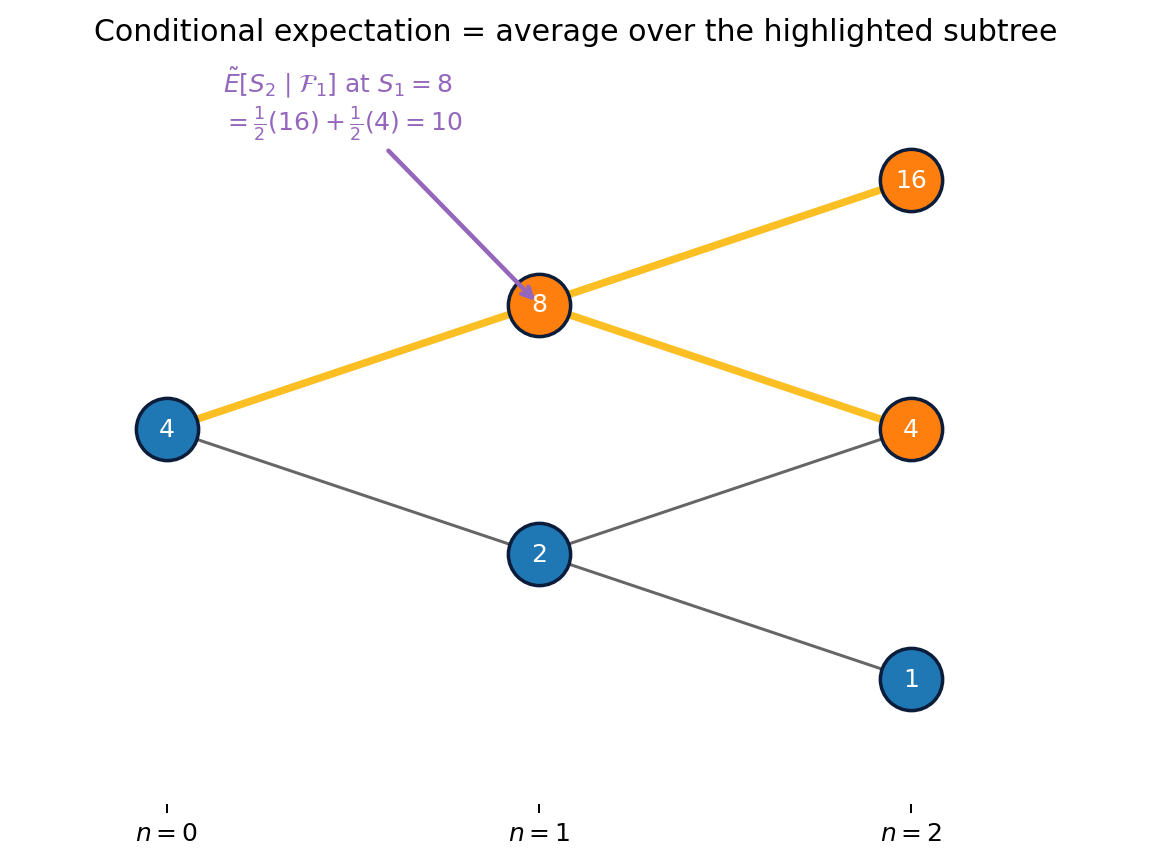
\includegraphics[keepaspectratio]{figures/ch00-cond-exp-subtree.png}}
\caption{A 2-period tree under Toy, with the subtree rooted at the upper
time-1 node \(S_1=8\) highlighted. The arrow labels
``\(\tilde{\mathbb{E}}[X \mid \mathcal{F}_1]\) = probability-weighted
average over the shaded subtree.'' This is conditional expectation in
one picture.}
\end{figure}

\begin{figure}
\centering
\pandocbounded{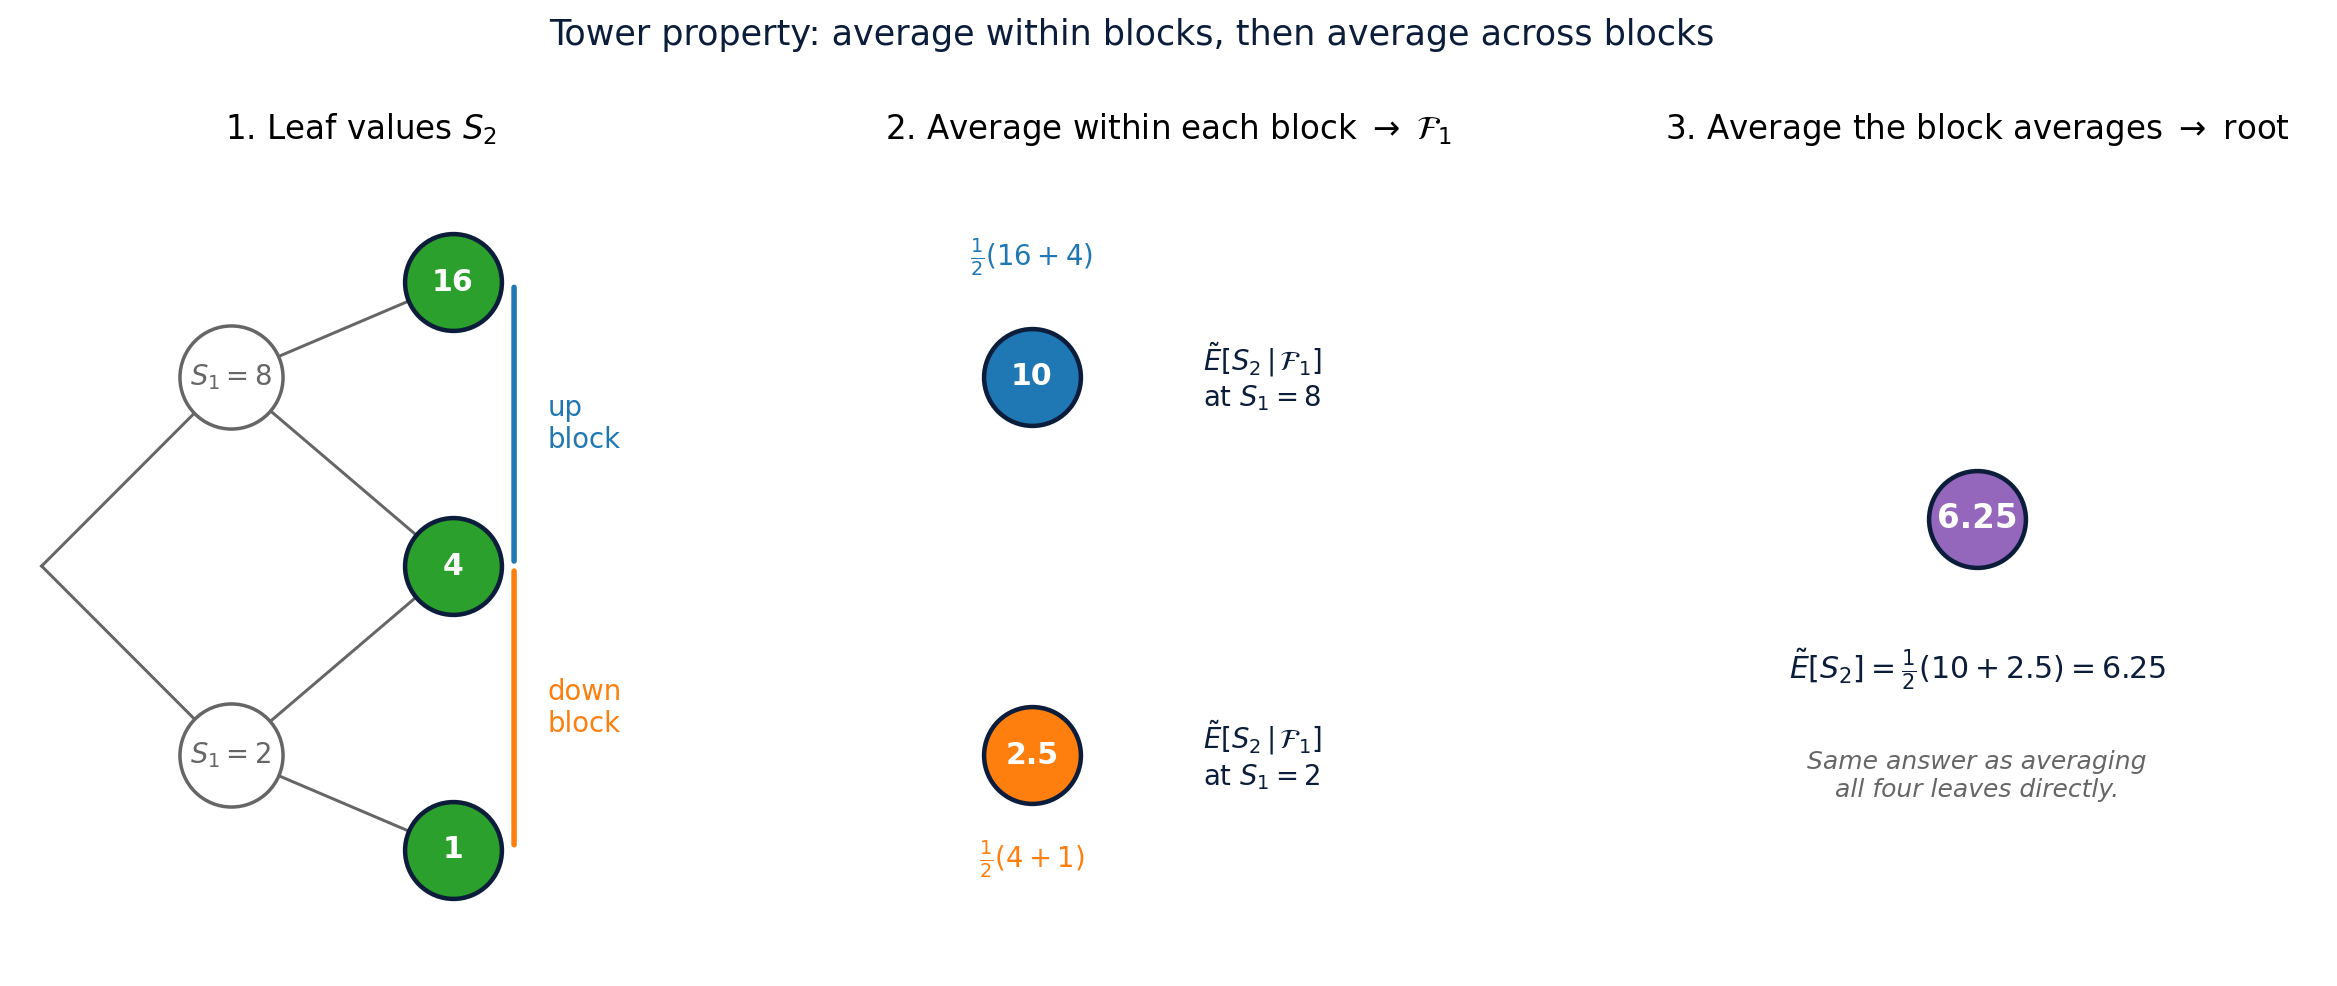
\includegraphics[keepaspectratio]{figures/ch00-tower-property.png}}
\caption{Three-panel storyboard of the tower property: panel 1 shows the
four leaf values of \(S_2\); panel 2 shows the two intermediate
conditional expectations at \(\mathcal{F}_1\); panel 3 shows the root
value as the average of the two. Each arrow is a ``fold'' --- averaging
within a partition block.}
\end{figure}

\subsection{0.6.3 Table}\label{table-3}

\textbf{Table 0.7.} Backward induction on the toy 3-period tree,
\(S_0 = 4\), \(u = 2\), \(d = 1/2\), \(\tilde p = 1/2\), \(r = 1/4\). A
node \((t, k)\) sits at time \(t\) with \(k\) up-moves so far. The
recombining tree has \(t+1\) distinct nodes at time \(t\).
\emph{Definition.} The right-most column gives
\(\tilde{\mathbb{E}}[S_3 \mid \text{node}] = S \cdot (1+r)^{\,3-t}\);
for leaf rows (\(t = 3\)) it degenerates to \(S\) itself.

{\def\LTcaptype{none} % do not increment counter
\begin{table}[H]
\centering
\begin{tabular}{|c|c|r|c|r|}
\toprule
\((t,k)\) & label & \(S\) & paths & \(\tilde{\mathbb{E}}[S_3 \mid \text{node}]\) \\
\midrule



\((0,0)\) & root & \(4\) & \(1\) & \(7.8125\) \\
\((1,1)\) & U & \(8\) & \(1\) & \(12.500\) \\
\((1,0)\) & D & \(2\) & \(1\) & \(3.125\) \\
\((2,2)\) & UU & \(16\) & \(1\) & \(20.000\) \\
\((2,1)\) & UD/DU & \(4\) & \(2\) & \(5.000\) \\
\((2,0)\) & DD & \(1\) & \(1\) & \(1.250\) \\
\((3,3)\) & leaf & \(32\) & \(1\) & \(32.000\) \\
\((3,2)\) & leaf & \(8\) & \(3\) & \(8.000\) \\
\((3,1)\) & leaf & \(2\) & \(3\) & \(2.000\) \\
\((3,0)\) & leaf & \(0.5\) & \(1\) & \(0.500\) \\
\bottomrule
\end{tabular}
\end{table}
}

Row checks: \((0,0)\): \(4 \cdot 1.25^3 = 7.8125\). \((1,1)\):
\(8 \cdot 1.25^2 = 12.5\). \((1,0)\): \(2 \cdot 1.25^2 = 3.125\).
\((2,k)\): \(S \cdot 1.25\) in each row. Leaf rows trivially return
\(S\).

Two things to read off the table.

\textbf{The expected price grows at the rate \(r\) per period.} Under
risk-neutral measure,
\(\tilde{\mathbb{E}}[S_n \mid S_m] = S_m \,(1+r)^{n-m}\). That's why the
root's expected value of \(S_3\) is \(7.8125 = 4 \cdot (1.25)^3\), not
\(4\). The ``martingale'' object is \emph{discounted} price
\(S_n/(1+r)^n\), which has constant expectation --- not raw price. We'll
prove this properly in Chapter 3.

\textbf{The tower property holds level by level.}
\(7.8125 = (1/2)(12.5) + (1/2)(3.125)\) ✓ at the root.
\(12.5 = (1/2)(20) + (1/2)(5)\) ✓ at node U.
\(3.125 = (1/2)(5) + (1/2)(1.25)\) ✓ at node D. Each level is the
probability-weighted average of the level below --- averaging in stages
gives the same answer as averaging once.

\subsection{0.6.4 Exercises}\label{exercises-5}

\begin{enumerate}
\def\labelenumi{\arabic{enumi}.}
\tightlist
\item
  Toy, 3-period, \(\tilde{\mathbb{E}}[S_3 \mid S_1 = 8]\).
  \textbf{Answer:} \(12.5\).
\item
  Same tree, \(\tilde{\mathbb{E}}[S_3 \mid S_2 = 4]\). \textbf{Answer:}
  \(5\) (mean of \(\{8, 2\}\)).
\item
  Verify the tower at the root: \(7.8125 = (1/2)(12.5) + (1/2)(3.125)\).
  \textbf{Answer:} \(7.8125\). ✓
\end{enumerate}

\begin{center}\rule{0.5\linewidth}{0.5pt}\end{center}

\section{§0.7 Counting Lattice Paths --- Reflection Principle
Prep}\label{counting-lattice-paths-reflection-principle-prep}

\textbf{Punchline.} A \emph{path} is a sequence of \(\pm 1\) steps. The
number of paths from \((0,0)\) to \((n, k)\) is \(\binom{n}{(n+k)/2}\)
--- choose which steps were ups. To count paths that \emph{touch} a
barrier level \(L\), \textbf{reflect} them across \(L\) --- you get a
bijection to paths ending somewhere else, and bijections preserve
counts. This is the entire content of Chapter 5's reflection principle,
pre-rehearsed here on small examples.

\textbf{Intuition.} Picture a path on a sheet of grid paper, walking
right one step at a time and either up or down each step. If a path
\emph{touches} the line \(y = L\) at some point, take a mirror, lay it
flat on the line \(y = L\), and reflect everything \emph{after} the
first touch. You get a different path, but with the same number of
steps, that ends at \(2L - h\) (where \(h\) was the original endpoint).
The reflection is a bijection: every ``touching path'' corresponds to
exactly one ``ends-at-\(2L-h\)'' path, and vice versa. Counting one
tells you the count of the other.

\subsection{0.7.1 Definitions}\label{definitions-4}

A \textbf{lattice path} of length \(n\) starting at \((0, 0)\) is a
sequence \(X_0 = 0\), \(X_1, X_2, \dots, X_n\) with each step
\(X_t - X_{t-1} \in \{+1, -1\}\). Each path corresponds to a unique
sequence of \(n\) U's and D's. There are \(2^n\) paths of length \(n\)
in total.

\textbf{Endpoint formula.} A path of length \(n\) ends at level \(k\)
iff it has \(u\) up-steps and \(d\) down-steps with \(u - d = k\),
\(u + d = n\), so \(u = (n + k)/2\). Therefore

\[\#\{\text{paths from } (0, 0) \text{ to } (n, k)\} \;=\; \binom{n}{(n+k)/2}, \qquad k \in \{-n, -n+2, \dots, n-2, n\}.\]

(If \((n + k)/2\) is not a non-negative integer \(\leq n\), the count is
zero.)

\textbf{Reflection principle (stated, illustrated below).} Fix a level
\(L > 0\). Let \(h\) be an integer with \(h < L\). The number of paths
from \((0, 0)\) to \((n, h)\) that touch the level \(L\) somewhere along
the way equals the number of paths from \((0, 0)\) to \((n, 2L - h)\):

\[\#\{\text{paths to } (n, h) \text{ touching } L\} \;=\; \#\{\text{paths to } (n, 2L - h)\} \;=\; \binom{n}{(n + 2L - h)/2}.\]

The bijection: for any touching path, locate the \emph{first} time
\(\tau\) it hits \(L\), then reflect the segment after \(\tau\) across
\(L\). The reflected segment ends at \(2L - h\) instead of \(h\);
everything before \(\tau\) is unchanged. Reversing the reflection gives
the inverse map. Same count.

\textbf{Ballot identity.} Among paths of length \(n\) ending at
\(k > 0\), the number that stay strictly positive for \(t \geq 1\) is

\[\frac{k}{n} \binom{n}{(n+k)/2}.\]

This is \emph{Bertrand's ballot problem} and we will use it in Chapter 5
for first-passage counting.

\subsection{0.7.2 Examples}\label{examples-6}

\textbf{Example 0.7.1 (counting paths to an endpoint).} Paths of length
6 ending at level \(+2\): that's \(u = 4\) up-steps and \(d = 2\)
down-steps. Count: \(\binom{6}{4} = 15\).

\textbf{Example 0.7.2 (reflection identity).} Paths of length 6 ending
at \(+2\) that \emph{touch} level \(+3\). By reflection, this equals the
count of paths ending at \(2 \cdot 3 - 2 = +4\). That count is
\(\binom{6}{5} = 6\).

\textbf{Example 0.7.3 (read off the complement).} Paths of length 6
ending at \(+2\) that \emph{do not} touch \(+3\): \(15 - 6 = 9\). So
60\% of paths to \(+2\) touched \(+3\) along the way.

\textbf{Example 0.7.4 (ballot count).} Paths of length 10 ending at
\(+4\) that stay strictly positive from \(t = 1\) onwards. By ballot:
\((4/10) \binom{10}{7} = 0.4 \cdot 120 = 48\). Out of
\(\binom{10}{7} = 120\) total paths to \(+4\), exactly 48 stayed
strictly above zero.

\textbf{Example 0.7.5 (small enumeration, \(n = 4\)).} Enumerate every
length-4 path and tabulate the endpoints. There are \(2^4 = 16\) paths.
By endpoint:

{\def\LTcaptype{none} % do not increment counter
\begin{table}[H]
\centering
\begin{tabular}{|r|r|r|}
\toprule
Endpoint \(k\) & Count & \(\binom{4}{(4+k)/2}\) \\
\midrule



\(-4\) & \(1\) & \(1\) \\
\(-2\) & \(4\) & \(4\) \\
\(0\) & \(6\) & \(6\) \\
\(+2\) & \(4\) & \(4\) \\
\(+4\) & \(1\) & \(1\) \\
\bottomrule
\end{tabular}
\end{table}
}

Endpoint \(-4\) is the unique path DDDD; endpoint \(+4\) is UUUU. Sum is
\(16\). ✓ Row 4 of Pascal's triangle is reproduced.

\textbf{Example 0.7.6 (max of a length-4 walk).} Compute
\(\mathbb{P}\!\left(\max_{1 \le t \le 4} X_t \geq 2\right)\) for the
fair symmetric walk. We split ``paths that reach \(+2\)'' into two
disjoint classes:

\begin{itemize}
\tightlist
\item
  \textbf{End at or above \(+2\)} (trivially touch \(+2\)): endpoint
  \(h \in \{+2, +4\}\).
\item
  \textbf{End strictly below \(+2\) but touch it} (endpoint
  \(h \in \{0, -2, -4\}\)): for these, \emph{reflection} identifies them
  one-to-one with paths ending at \(4 - h\).
\end{itemize}

{\def\LTcaptype{none} % do not increment counter
\begin{table}[H]
\centering
\begin{tabular}{|c|c|l|c|c|}
\toprule
End at \(h\) & Count to \(h\) & Touch \(+2\)? & Refl. \(4-h\) & Touch
count \\
\midrule



\(+4\) & \(1\) & yes & & \(1\) \\
\(+2\) & \(4\) & yes & & \(4\) \\
\(0\) & \(6\) & some & \(+4\) & \(1\) \\
\(-2\) & \(4\) & some & \(+6\) & \(0\) \\
\(-4\) & \(1\) & some & \(+8\) & \(0\) \\
\bottomrule
\end{tabular}
\end{table}
}

\emph{Legend.} yes = trivially touches (endpoint already \(\geq +2\));
some = only the touching subset, counted by reflection. \emph{Counts.}
End-counts come from \(\binom{4}{(4+h)/2}\) (rows: \(1,4,6,4,1\)).
Reflected-touch counts come from \(\binom{4}{(4+\text{refl})/2}\): refl
\(+4 \to \binom{4}{4}=1\); refl \(+6 \to \binom{4}{5}=0\); refl
\(+8 \to 0\). Blank in ``Refl.'' column = no reflection needed.

The last column sums to \(1 + 4 + 1 + 0 + 0 = 6\). So \(6\) of the
\(16\) length-4 paths touch level \(+2\), giving

\[\mathbb{P}\!\left(\max_{1 \le t \le 4} X_t \geq 2\right) \;=\; \frac{6}{16} \;=\; \frac{3}{8}.\]

\textbf{Direct enumeration check.} All length-4 paths that touch \(+2\),
listed by their step sequence:

\[\{\text{UUUU},\ \text{UUUD},\ \text{UUDU},\ \text{UUDD},\ \text{UDUU},\ \text{DUUU}\}.\]

Verify: any path starting UU touches \(+2\) at \(t = 2\) (that's the
four paths UUUU/UUUD/UUDU/UUDD); UDUU reaches \(+2\) at \(t = 4\) via
levels \(1, 0, 1, 2\); DUUU reaches \(+2\) at \(t = 4\) via
\(-1, 0, 1, 2\). Six paths total. ✓

The reflection principle gave the same count via algebra, without
listing paths. For \(n = 4\) that's still a manageable enumeration; for
\(n = 40\) we'd have \(2^{40} \approx 10^{12}\) paths and reflection is
the only feasible route.

\textbf{Example 0.7.7 (the reflection bijection in pictures).} Take the
path UUDDD on \(n = 5\), which ends at \(-1\) but touches \(+2\) at
\(t = 2\). The first touch of \(+2\) is at \(t = 2\). Reflect the
segment from \(t = 2\) onwards (which traces levels \(2, 1, 0, -1\) at
steps \(t = 2, 3, 4, 5\)) across \(y = 2\) --- it now visits
\(2, 3, 4, 5\). The reflected path is UUUUU, ending at \(+5\).

The reflection principle predicts: count of paths to \(-1\) touching
\(+2\) \(=\) count of paths to \(+5 = \binom{5}{5} = 1\). So exactly
\(1\) of the \(\binom{5}{2}=10\) paths ending at \(-1\) touches \(+2\),
and that path is UUDDD itself.

\begin{figure}
\centering
\pandocbounded{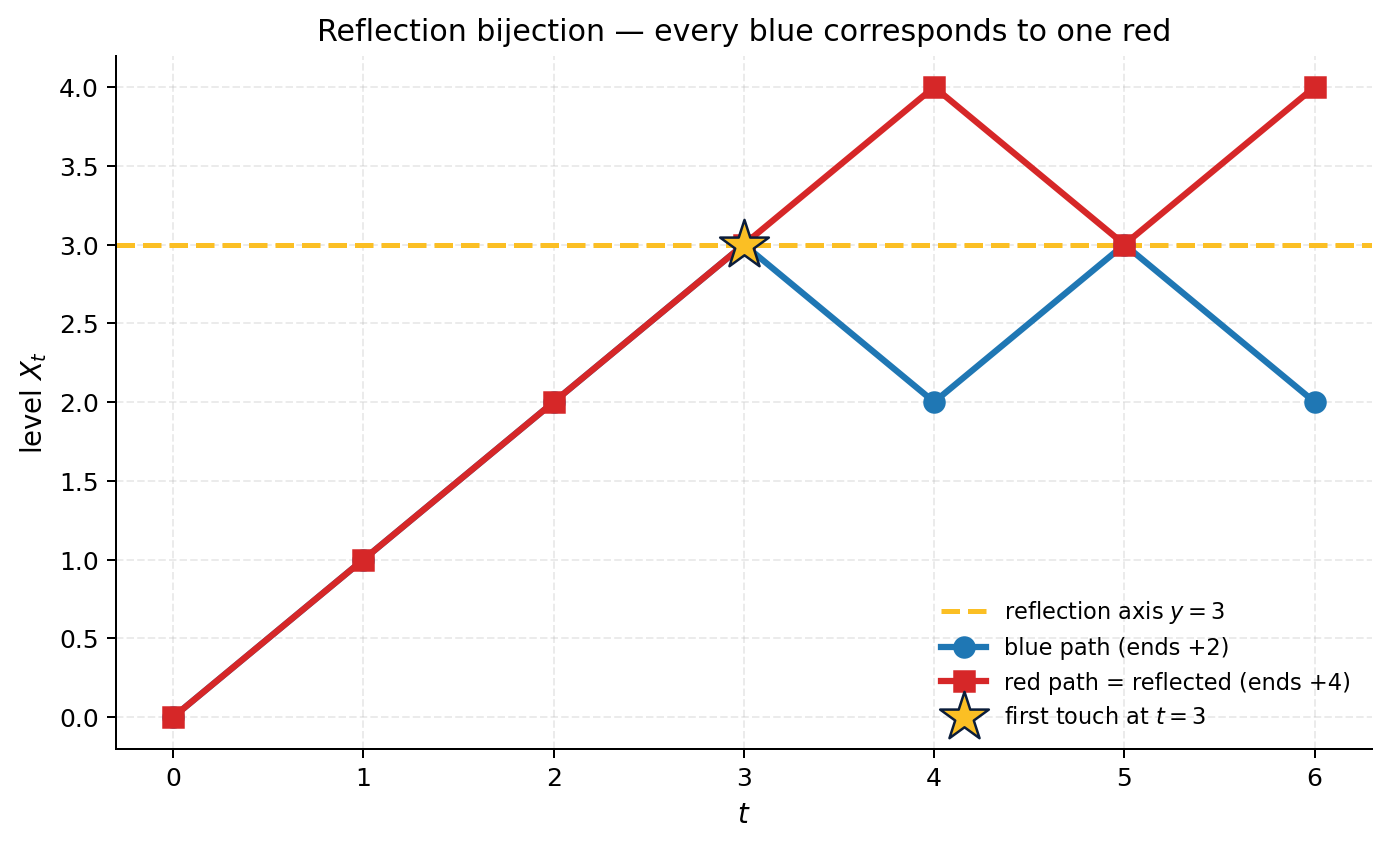
\includegraphics[keepaspectratio]{figures/ch00-reflection-bijection.png}}
\caption{A single length-6 path that first touches level \(+3\) at
\(t = 3\) (shown in blue), and its post-touch reflection across
\(y = +3\) (shown in red). The blue path ends at \(+2\); the red path
ends at \(+4\). They share the first 3 steps; they are mirror images on
\([3, 6]\). The ``first-touch'' point at \(t = 3\) is marked with a
star. The bijection says: every blue path counts a red one, and vice
versa.}
\end{figure}

\begin{figure}
\centering
\pandocbounded{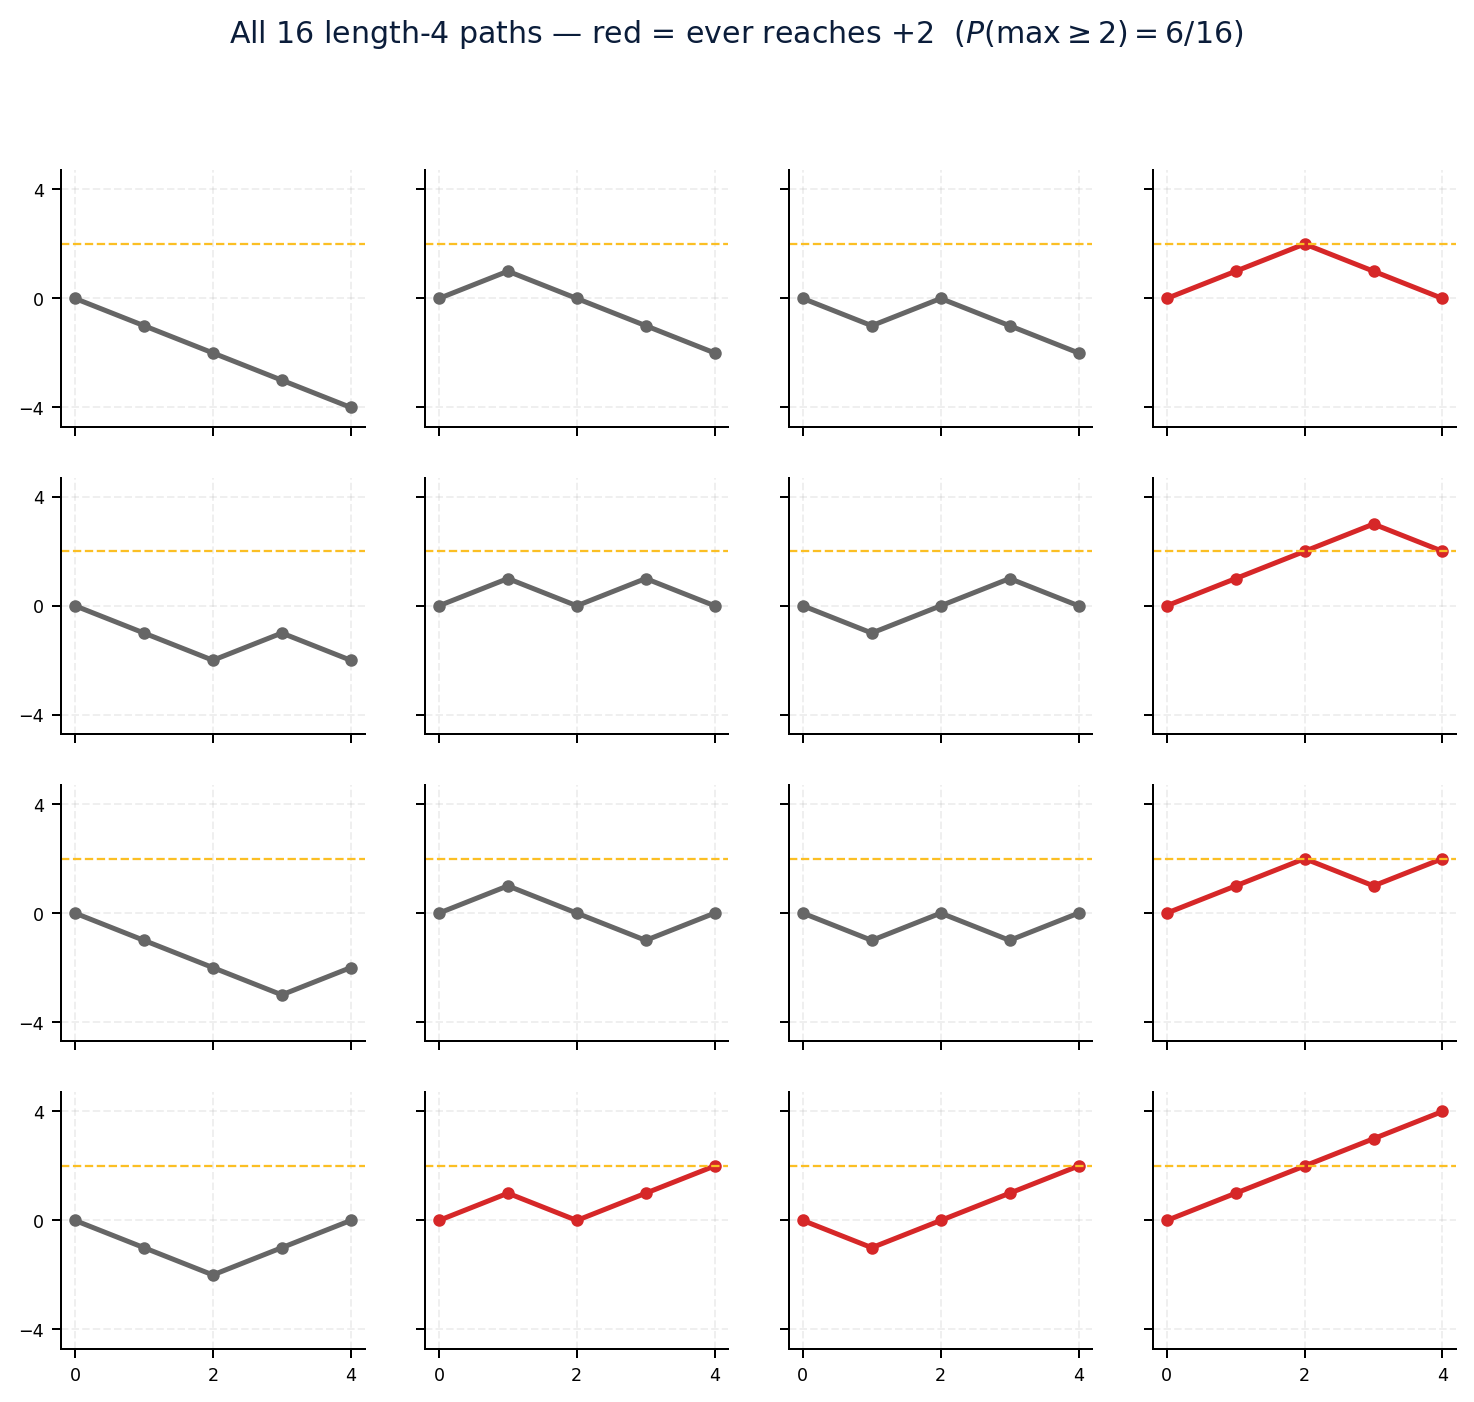
\includegraphics[keepaspectratio]{figures/ch00-all-16-paths.png}}
\caption{Small-multiples grid of all 16 paths of length 4 on a \(\pm 1\)
lattice. Paths that ever reach level \(+2\) are coloured red; paths that
don't are grey. The six red paths give
\(\mathbb{P}(\max \geq 2) = 6/16 = 3/8\), matching the
reflection-principle count above.}
\end{figure}

\begin{figure}
\centering
\pandocbounded{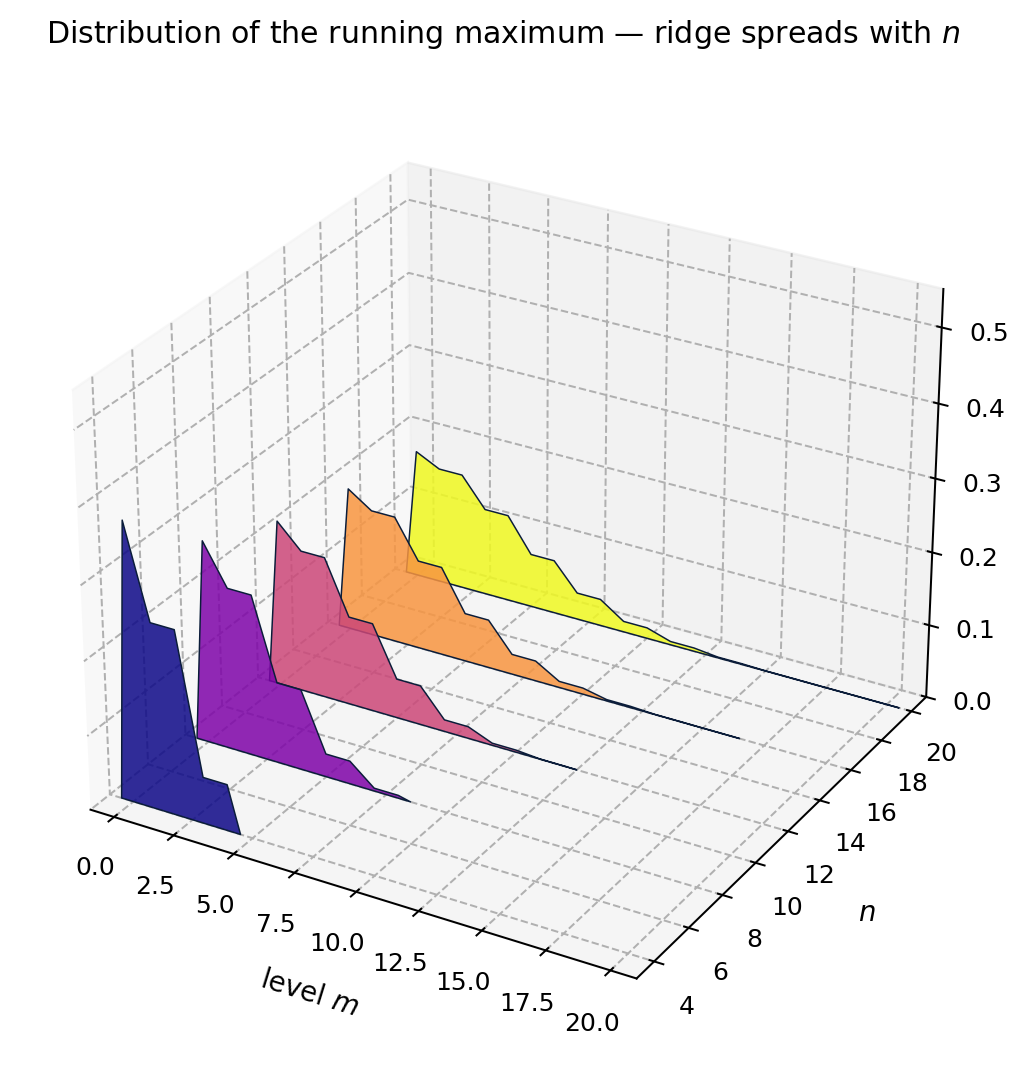
\includegraphics[keepaspectratio]{figures/ch00-max-distribution-3d.png}}
\caption{3-D bar plot of the maximum-level distribution
\(\mathbb{P}(\max_{1 \le t \le n} X_t = m)\) for
\(n \in \{4, 8, 12, 16, 20\}\) on a fair symmetric walk. The ridge moves
out and broadens with \(n\) --- exactly the scaling the reflection
principle predicts and that Chapter 5 will use to derive distributional
facts about the running maximum.}
\end{figure}

\subsection{0.7.3 Tables}\label{tables-2}

\textbf{Table 0.8.} Path counts \((n, k)\) for \(n = 0, 2, 4, 6, 8, 10\)
(even parity rows). Entries are \(\binom{n}{(n+k)/2}\).

{\def\LTcaptype{none} % do not increment counter
\begin{table}[H]
\centering
\begin{tabular}{|r|r|r|r|r|r|r|r|r|r|r|r|}
\toprule
\(n \backslash k\) & \(-10\) & \(-8\) & \(-6\) & \(-4\) & \(-2\) & \(0\) & \(+2\) & \(+4\) & \(+6\) & \(+8\) & \(+10\) \\
\midrule



\(0\) & & & & & & \(1\) & & & & & \\
\(2\) & & & & & \(1\) & \(2\) & \(1\) & & & & \\
\(4\) & & & & \(1\) & \(4\) & \(6\) & \(4\) & \(1\) & & & \\
\(6\) & & & \(1\) & \(6\) & \(15\) & \(20\) & \(15\) & \(6\) & \(1\) &
& \\
\(8\) & & \(1\) & \(8\) & \(28\) & \(56\) & \(70\) & \(56\) & \(28\) &
\(8\) & \(1\) & \\
\(10\) & \(1\) & \(10\) & \(45\) & \(120\) & \(210\) & \(252\) & \(210\)
& \(120\) & \(45\) & \(10\) & \(1\) \\
\bottomrule
\end{tabular}
\end{table}
}

\textbf{Table 0.9.} Reflection-count check for paths of length \(6\)
ending at \(h = 2\), across barrier levels \(L\).

{\def\LTcaptype{none} % do not increment counter
\begin{table}[H]
\centering
\begin{tabular}{|r|r|r|r|}
\toprule
Barrier \(L\) & Refl. \(2L - h\) & Touch count & Fraction \\
\midrule



\(L = 2\) & \(2\) & \(15\) & \(1.00\) \\
\(L = 3\) & \(4\) & \(6\) & \(0.40\) \\
\(L = 4\) & \(6\) & \(1\) & \(0.07\) \\
\(L = 5\) & \(8\) & \(0\) & \(0.00\) \\
\bottomrule
\end{tabular}
\end{table}
}

Row computations: \(L=2\): trivially all \(15\) paths touch (endpoint
\(h=2\) is already on the barrier). \(L=3\): \(\binom{6}{5}=6\).
\(L=4\): \(\binom{6}{6}=1\). \(L=5\): refl \(8 > 6\), impossible.

\subsection{0.7.4 Exercises}\label{exercises-6}

\begin{enumerate}
\def\labelenumi{\arabic{enumi}.}
\tightlist
\item
  Number of paths of length 8 ending at \(+4\). \textbf{Answer:}
  \(\binom{8}{6} = 28\).
\item
  Number of paths of length 8 ending at \(+4\) that touch \(+5\).
  \textbf{Answer:} \(\binom{8}{6.5}\) --- wait, \((8 + 6)/2 = 7\), so
  \(\binom{8}{7} = 8\) (reflect \(+4 \to 2 \cdot 5 - 4 = 6\)).
\item
  Number of paths of length 8 ending at \(0\) that stay strictly
  positive at every interior step. \textbf{Answer:} This is the Catalan
  number \(C_4 = 14\).
\end{enumerate}

\begin{center}\rule{0.5\linewidth}{0.5pt}\end{center}

\section{§0.8 The Binomial
Distribution}\label{the-binomial-distribution}

\textbf{Punchline.} \(H \sim \mathrm{Bin}(n, p)\) counts heads in \(n\)
independent coin flips. Its PMF is \(\binom{n}{k} p^k (1-p)^{n-k}\),
mean \(np\), variance \(np(1-p)\). The pricing formula in Chapter 7 is
\emph{literally} a sum of binomial probabilities times payoffs --- so
the binomial distribution is the engine room.

\textbf{Intuition.} Each flip is a tiny Bernoulli random variable; \(H\)
is just their sum. Linearity of \(\mathbb{E}\) gives the mean: \(n\)
flips times \(p\) heads per flip \(= np\). Independence gives the
variance: \(n\) flips times \(p(1-p)\) variance per flip \(= np(1-p)\).
Everything else is rearranging \(\binom{n}{k}\).

\subsection{0.8.1 Definitions and facts}\label{definitions-and-facts}

If \(X_1, X_2, \dots, X_n\) are independent Bernoulli\((p)\) random
variables and \(H = X_1 + \dots + X_n\), then \(H\) is
\textbf{Binomial\((n, p)\)}:

\[\mathbb{P}(H = k) \;=\; \binom{n}{k}\, p^k\, (1-p)^{n-k}, \qquad k = 0, 1, \dots, n.\]

\textbf{Mean and variance}:

\[\mathbb{E}[H] = np, \qquad \mathrm{Var}(H) = np(1-p), \qquad \sigma_H = \sqrt{np(1-p)}.\]

\textbf{Recurrence} (useful for tabulating the PMF without recomputing
factorials):

\[\frac{\mathbb{P}(H = k+1)}{\mathbb{P}(H = k)} \;=\; \frac{n - k}{k + 1} \cdot \frac{p}{1 - p}.\]

\textbf{Sum of independent binomials}: if
\(H_1 \sim \mathrm{Bin}(n_1, p)\) and \(H_2 \sim \mathrm{Bin}(n_2, p)\)
are independent, then \(H_1 + H_2 \sim \mathrm{Bin}(n_1 + n_2, p)\).

\subsection{0.8.2 Examples}\label{examples-7}

\textbf{Example 0.8.1 (Bin\((5, 0.5)\) PMF, all six values).}

{\def\LTcaptype{none} % do not increment counter
\begin{table}[H]
\centering
\begin{tabular}{|r|r|r|}
\toprule
\(k\) & \(\binom{5}{k}\) & \(\mathbb{P}(H = k) = \binom{5}{k}/32\) \\
\midrule



\(0\) & \(1\) & \(0.03125\) \\
\(1\) & \(5\) & \(0.15625\) \\
\(2\) & \(10\) & \(0.31250\) \\
\(3\) & \(10\) & \(0.31250\) \\
\(4\) & \(5\) & \(0.15625\) \\
\(5\) & \(1\) & \(0.03125\) \\
\bottomrule
\end{tabular}
\end{table}
}

Mean \(= 2.5\), variance \(= 1.25\), \(\sigma = 1.118\).

\textbf{Example 0.8.2 (Bin\((10, 0.6)\), central probability).}

\[\mathbb{P}(H = 6) \;=\; \binom{10}{6} \cdot 0.6^6 \cdot 0.4^4 \;=\; 210 \cdot 0.04666 \cdot 0.0256 \;=\; 0.2508.\]

Compare with the mean \(\mathbb{E}[H] = 6\): the most likely outcome is
exactly the mean, with probability about \(25\%\).

\textbf{Example 0.8.3 (mean and variance).} Bin\((10, 0.6)\):
\(\mathbb{E} = 6\), \(\mathrm{Var} = 10 \cdot 0.6 \cdot 0.4 = 2.4\),
\(\sigma = 1.549\).

\textbf{Example 0.8.4 (recurrence in action).} From 0.8.2,
\(\mathbb{P}(H = 6) = 0.2508\). Then

\[\mathbb{P}(H = 7) \;=\; 0.2508 \cdot \frac{10 - 6}{6 + 1} \cdot \frac{0.6}{0.4} \;=\; 0.2508 \cdot \frac{4}{7} \cdot 1.5 \;=\; 0.2150.\]

Direct:
\(\binom{10}{7} \cdot 0.6^7 \cdot 0.4^3 = 120 \cdot 0.02799 \cdot 0.064 = 0.2150\).
✓

\textbf{Example 0.8.5 (Toy, risk-neutral terminal distribution).}
\(S_0 = 4\), \(u = 2\), \(d = 1/2\), \(\tilde p = 1/2\), \(n = 3\). Then
\(S_3 = 4 \cdot u^H d^{3 - H}\) where \(H \sim \mathrm{Bin}(3, 1/2)\).

{\def\LTcaptype{none} % do not increment counter
\begin{table}[H]
\centering
\begin{tabular}{|r|r|r|}
\toprule
\(H = k\) & \(S_3\) & \(\tilde{\mathbb{P}}(H = k) = \binom{3}{k}/8\) \\
\midrule



\(0\) & \(1/2\) & \(1/8 = 0.125\) \\
\(1\) & \(2\) & \(3/8 = 0.375\) \\
\(2\) & \(8\) & \(3/8 = 0.375\) \\
\(3\) & \(32\) & \(1/8 = 0.125\) \\
\bottomrule
\end{tabular}
\end{table}
}

\(\tilde{\mathbb{E}}[S_3] = 0.125 \cdot 0.5 + 0.375 \cdot 2 + 0.375 \cdot 8 + 0.125 \cdot 32 = 0.0625 + 0.75 + 3 + 4 = 7.8125 = 4 \cdot (1.25)^3\).
✓ (Discount at \((1+r)^3 = (5/4)^3 = 1.953\):
\(7.8125 / 1.953 = 4 = S_0\).)

\textbf{Example 0.8.6 (call ITM probability, realistic).} \(S_0 = 100\),
\(K = 100\), \(u = 1.10\), \(d = 0.90\), \(n = 3\), \(\tilde p = 0.6\).
The call is in-the-money iff \(S_3 > 100\), i.e., iff \(H \geq 2\) (with
\(H = 2\) giving \(S_3 = 100 \cdot 1.21 \cdot 0.9 = 108.9 > 100\) and
\(H = 1\) giving \(S_3 = 100 \cdot 1.1 \cdot 0.81 = 89.1 < 100\)). So

\[\tilde{\mathbb{P}}(H \geq 2) \;=\; \binom{3}{2} \cdot 0.6^2 \cdot 0.4 + 0.6^3 \;=\; 3 \cdot 0.144 + 0.216 \;=\; 0.432 + 0.216 \;=\; 0.648.\]

\textbf{Example 0.8.7 (cumulative tail).} Bin\((20, 0.5)\): probability
of at least 15 heads. \(\binom{20}{15} = 15504\),
\(\binom{20}{16} = 4845\), \(\binom{20}{17} = 1140\),
\(\binom{20}{18} = 190\), \(\binom{20}{19} = 20\),
\(\binom{20}{20} = 1\). Sum \(= 21700\). Total
\(2^{20} = 1{,}048{,}576\). So
\(\mathbb{P}(H \geq 15) = 21700/1048576 \approx 0.02069\).

\begin{figure}
\centering
\pandocbounded{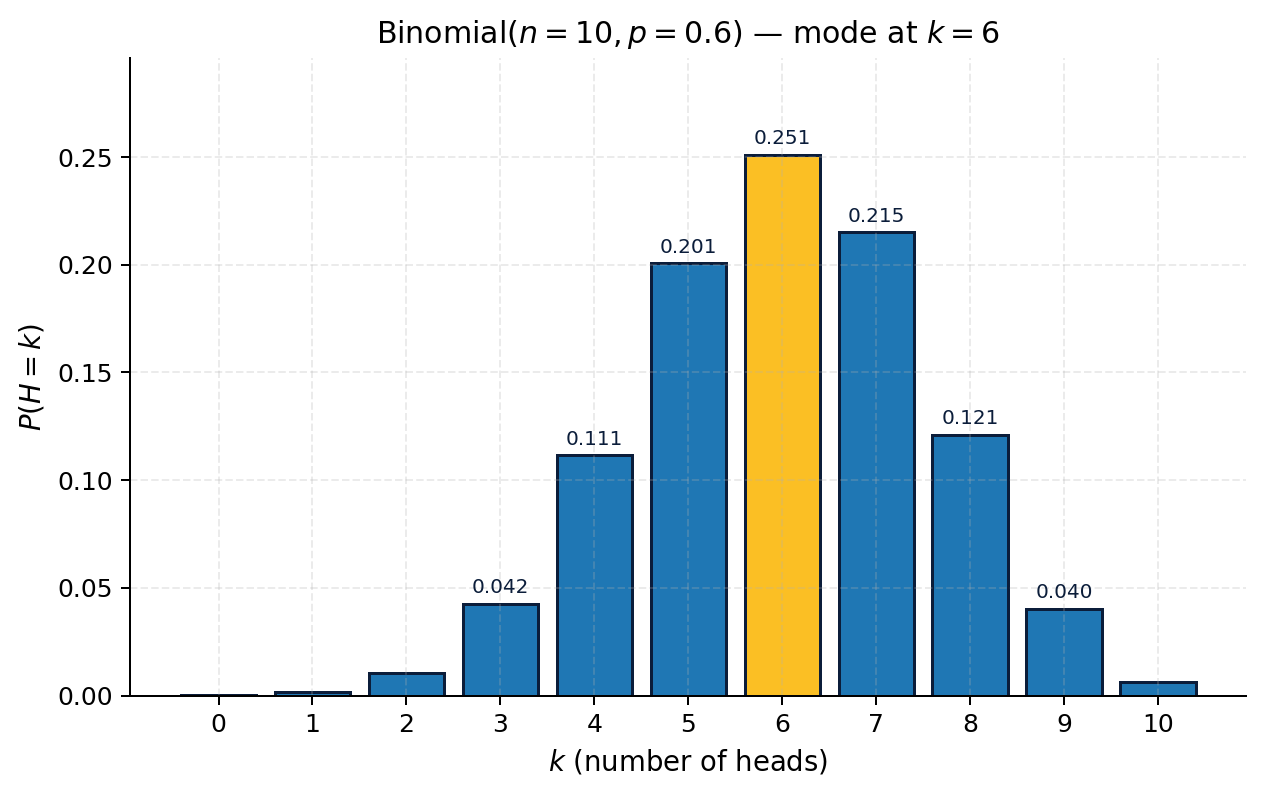
\includegraphics[keepaspectratio]{figures/ch00-binom-10-06-pmf.png}}
\caption{Binomial PMF for Bin\((10, 0.6)\): bar chart of
\(\mathbb{P}(H = k)\) for \(k = 0, \dots, 10\). The mode is at \(k = 6\)
(the mean), with probability \(\approx 0.25\).}
\end{figure}

\begin{figure}
\centering
\pandocbounded{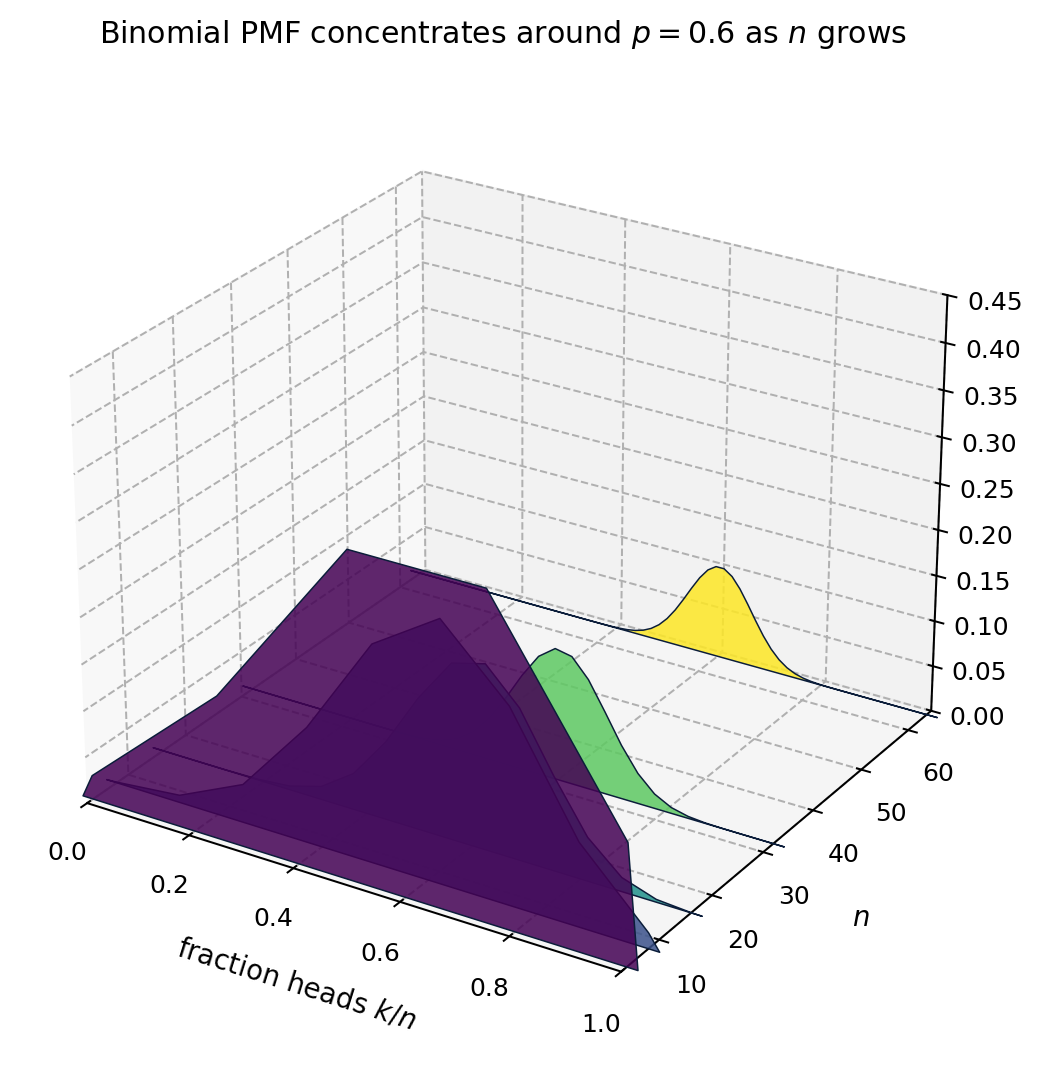
\includegraphics[keepaspectratio]{figures/ch00-binom-stacked-3d.png}}
\caption{3-D ridge plot of the Binomial PMF stacked across
\(n \in \{4, 8, 16, 32, 64\}\) (rescaled so each has the same \(x\) axis
of ``fraction heads''). As \(n\) grows, the PMF concentrates around
\(p = 0.6\) and becomes bell-shaped. This is the visual preview of the
Central Limit Theorem in §0.10 and the bridge to Black--Scholes in
Chapter 7.}
\end{figure}

\subsection{0.8.3 Tables}\label{tables-3}

\textbf{Table 0.10.} Binomial PMF for \(n = 10\), across four values of
\(p\).

{\def\LTcaptype{none} % do not increment counter
\begin{table}[H]
\centering
\begin{tabular}{|r|r|r|r|r|}
\toprule
\(k\) & \(p = 0.3\) & \(p = 0.5\) & \(p = 0.6\) & \(p = 0.7\) \\
\midrule



\(0\) & \(0.02825\) & \(0.00098\) & \(0.00010\) & \(0.00001\) \\
\(1\) & \(0.12106\) & \(0.00977\) & \(0.00157\) & \(0.00014\) \\
\(2\) & \(0.23347\) & \(0.04395\) & \(0.01062\) & \(0.00145\) \\
\(3\) & \(0.26683\) & \(0.11719\) & \(0.04247\) & \(0.00900\) \\
\(4\) & \(0.20012\) & \(0.20508\) & \(0.11148\) & \(0.03676\) \\
\(5\) & \(0.10292\) & \(0.24609\) & \(0.20066\) & \(0.10292\) \\
\(6\) & \(0.03676\) & \(0.20508\) & \(0.25082\) & \(0.20012\) \\
\(7\) & \(0.00900\) & \(0.11719\) & \(0.21499\) & \(0.26683\) \\
\(8\) & \(0.00145\) & \(0.04395\) & \(0.12093\) & \(0.23347\) \\
\(9\) & \(0.00014\) & \(0.00977\) & \(0.04031\) & \(0.12106\) \\
\(10\) & \(0.00001\) & \(0.00098\) & \(0.00605\) & \(0.02825\) \\
Sum & \(1.00000\) & \(1.00000\) & \(1.00000\) & \(1.00000\) \\
\bottomrule
\end{tabular}
\end{table}
}

\subsection{0.8.4 Exercises}\label{exercises-7}

\begin{enumerate}
\def\labelenumi{\arabic{enumi}.}
\tightlist
\item
  Bin\((8, 0.5)\): \(\mathbb{P}(H \geq 5)\). \textbf{Answer:}
  \(93/256 = 0.3633\).
\item
  Mean and variance of Bin\((20, 0.3)\). \textbf{Answer:} \(6\),
  \(4.2\).
\item
  Use the recurrence to get \(\mathbb{P}(H = 4)\) in Bin\((8, 0.5)\)
  from \(\mathbb{P}(H = 3)\). \textbf{Answer:} \(70/256 = 0.2734\).
\end{enumerate}

\begin{center}\rule{0.5\linewidth}{0.5pt}\end{center}

\section{§0.9 The Normal Distribution as a Tabulated
Function}\label{the-normal-distribution-as-a-tabulated-function}

\textbf{Punchline.} \(\Phi(z)\) is the area under the bell curve from
\(-\infty\) to \(z\). It is a \emph{function you look up} --- exact
values are in the appendix Table 0.A at the end of this chapter. Every
Black--Scholes calculation in Chapter 7 is a table lookup.

\textbf{Intuition.} The standard normal distribution is the bell-shaped
curve that you've seen on every introductory statistics page. Its total
area under the curve is 1 (it's a probability density). \(\Phi(z)\) is
just \emph{the running area from the far left up to \(z\)}. At \(z = 0\)
(the center), half the area is to the left, so \(\Phi(0) = 0.5\). At
\(z = +\infty\), all the area is to the left, so \(\Phi(\infty) = 1\).
Everything else is a smooth interpolation that's been tabulated for
centuries.

\subsection{0.9.1 Definitions}\label{definitions-5}

The \textbf{standard normal density} is the defining curve

\[\phi(z) \;=\; \frac{1}{\sqrt{2\pi}} e^{-z^2/2}.\]

(You will never need to take rates of change of this curve or compute
its area as a calculus exercise. Treat it as a curve drawn on paper.)
The peak is at \(z = 0\) with height \(1/\sqrt{2\pi} \approx 0.399\). It
is symmetric: \(\phi(-z) = \phi(z)\).

\textbf{Where does the constant \(1/\sqrt{2\pi}\) come from?} (Heuristic
via Stirling.) State Stirling's approximation as a fact:

\[n! \;\approx\; n^n e^{-n} \sqrt{2\pi n} \qquad (n \text{ large}).\]

Apply it to the centre coefficient \(\binom{n}{n/2}\) at \(n = 2m\).
After cancellation,

\[\binom{2m}{m} \;\approx\; \frac{4^m}{\sqrt{\pi m}}, \qquad \text{so} \qquad \frac{1}{2^{2m}} \binom{2m}{m} \;\approx\; \frac{1}{\sqrt{\pi m}}.\]

That is the peak probability of a centred Bin\((2m, 1/2)\). Now rescale:
the standardised binomial has spacing
\(\Delta z = 2/\sqrt{2m} = \sqrt{2/m}\) between bars. Convert PMF to a
density at \(z = 0\) by dividing the peak probability by the spacing:

\[\text{density at } z = 0 \;\approx\; \frac{1/\sqrt{\pi m}}{\sqrt{2/m}} \;=\; \frac{1}{\sqrt{2\pi}}.\]

So the constant \(1/\sqrt{2\pi}\) is not pulled out of a hat --- it is
\emph{exactly} the rescaled peak height of the symmetric binomial. We
will see the rest of the bell shape emerge in §0.10.

The \textbf{standard normal cumulative distribution function (CDF)} is

\[\Phi(z) \;=\; \mathbb{P}(Z \leq z),\]

where \(Z\) is a standard normal random variable. It is the ``running
area under the bell curve from \(-\infty\) to \(z\).'' Treat \(\Phi\) as
a tabulated function --- Table 0.A at the end of this chapter is the
table.

\textbf{Symmetry:} \(\Phi(-z) = 1 - \Phi(z)\).

\textbf{Moments of the standard normal} (stated, not derived).

\begin{itemize}
\tightlist
\item
  \(\mathbb{E}[Z] = 0\).
\item
  \(\mathrm{Var}(Z) = \mathbb{E}[Z^2] = 1\).
\item
  \emph{All odd moments vanish by symmetry:}
  \(\mathbb{E}[Z^{2k+1}] = 0\) for every \(k \geq 0\).
\item
  \emph{Even moments} follow the double-factorial pattern
\end{itemize}

\[\mathbb{E}[Z^{2k}] \;=\; (2k - 1)!! \;=\; 1, \; 3, \; 15, \; 105, \; 945, \; \dots \quad (k = 1, 2, 3, \dots).\]

Here \((2k-1)!! = (2k-1)(2k-3)\cdots 3 \cdot 1\) is the product of odd
numbers down to 1. The pattern \(1, 3, 15, 105, 945\) recurs in every
formula that touches the Black--Scholes machinery; we will not derive
it, only quote it.

\textbf{Standardisation: the two-parameter family \(N(\mu, \sigma^2)\).}
A general normal random variable \(X \sim N(\mu, \sigma^2)\) has mean
\(\mu\) and variance \(\sigma^2\), and is built from the standard normal
by an affine rescaling:

\[X \;=\; \mu + \sigma Z, \qquad \text{equivalently} \qquad Z \;=\; \frac{X - \mu}{\sigma}.\]

Then

\[\mathbb{P}(X \leq x) \;=\; \mathbb{P}\!\left(Z \leq \frac{x - \mu}{\sigma}\right) \;=\; \Phi\!\left(\frac{x - \mu}{\sigma}\right).\]

Every probability involving a normal random variable reduces to a
\(\Phi\) lookup on the standardised value. There is \emph{one} table
(Table 0.A); the parameters \(\mu\) and \(\sigma\) only re-scale where
we read it.

\subsection{0.9.2 Examples}\label{examples-8}

\textbf{Example 0.9.1 (canonical values).} Five \(\Phi\) values every
reader should commit to memory:

{\def\LTcaptype{none} % do not increment counter
\begin{table}[H]
\centering
\begin{tabular}{|r|r|l|}
\toprule
\(z\) & \(\Phi(z)\) & Interpretation \\
\midrule



\(0.00\) & \(0.5000\) & symmetric peak \\
\(1.00\) & \(0.8413\) & one-sigma right of mean \\
\(1.645\) & \(0.9500\) & 95th percentile \\
\(1.960\) & \(0.9750\) & two-sided 95\% confidence \\
\(2.326\) & \(0.9900\) & 99th percentile \\
\bottomrule
\end{tabular}
\end{table}
}

\textbf{Example 0.9.2 (negative \(z\) via symmetry).}
\(\Phi(-0.5) = 1 - \Phi(0.5) = 1 - 0.6915 = 0.3085\). So
\(\mathbb{P}(Z \leq -0.5) = 30.85\%\).

\textbf{Example 0.9.3 (two-sided interval).}
\(\mathbb{P}(-1 \leq Z \leq 1) = \Phi(1) - \Phi(-1) = 0.8413 - 0.1587 = 0.6826\).
The 68\% rule.

\textbf{Example 0.9.4 (standardising).} \(X \sim N(100, 15^2)\).
\(\mathbb{P}(X \leq 130) = \Phi((130 - 100)/15) = \Phi(2) = 0.9772\).

\textbf{Example 0.9.5 (inverse lookup).} Find \(z\) with
\(\Phi(z) = 0.99\). From Table 0.A: \(z = 2.326\).

\textbf{Example 0.9.6 (annual log return).} Suppose annual log returns
are \(X \sim N(0.05, 0.20^2)\). Probability the return is negative:
\(\mathbb{P}(X < 0) = \Phi((0 - 0.05)/0.20) = \Phi(-0.25) = 1 - 0.5987 = 0.4013\).
So a \(5\%\) expected return with \(20\%\) vol has a \(40\%\) chance of
being negative in any given year.

\textbf{Example 0.9.7 (Black--Scholes preview).} Compute the BS-style
quantity \(\Phi(d_1) - \Phi(d_2)\) for \(d_1 = 0.30\), \(d_2 = 0.10\).
From Table 0.A: \(\Phi(0.30) = 0.6179\), \(\Phi(0.10) = 0.5398\). So
\(\Phi(d_1) - \Phi(d_2) = 0.0781\). We will see exactly this kind of
arithmetic in Chapter 7.

\begin{figure}
\centering
\pandocbounded{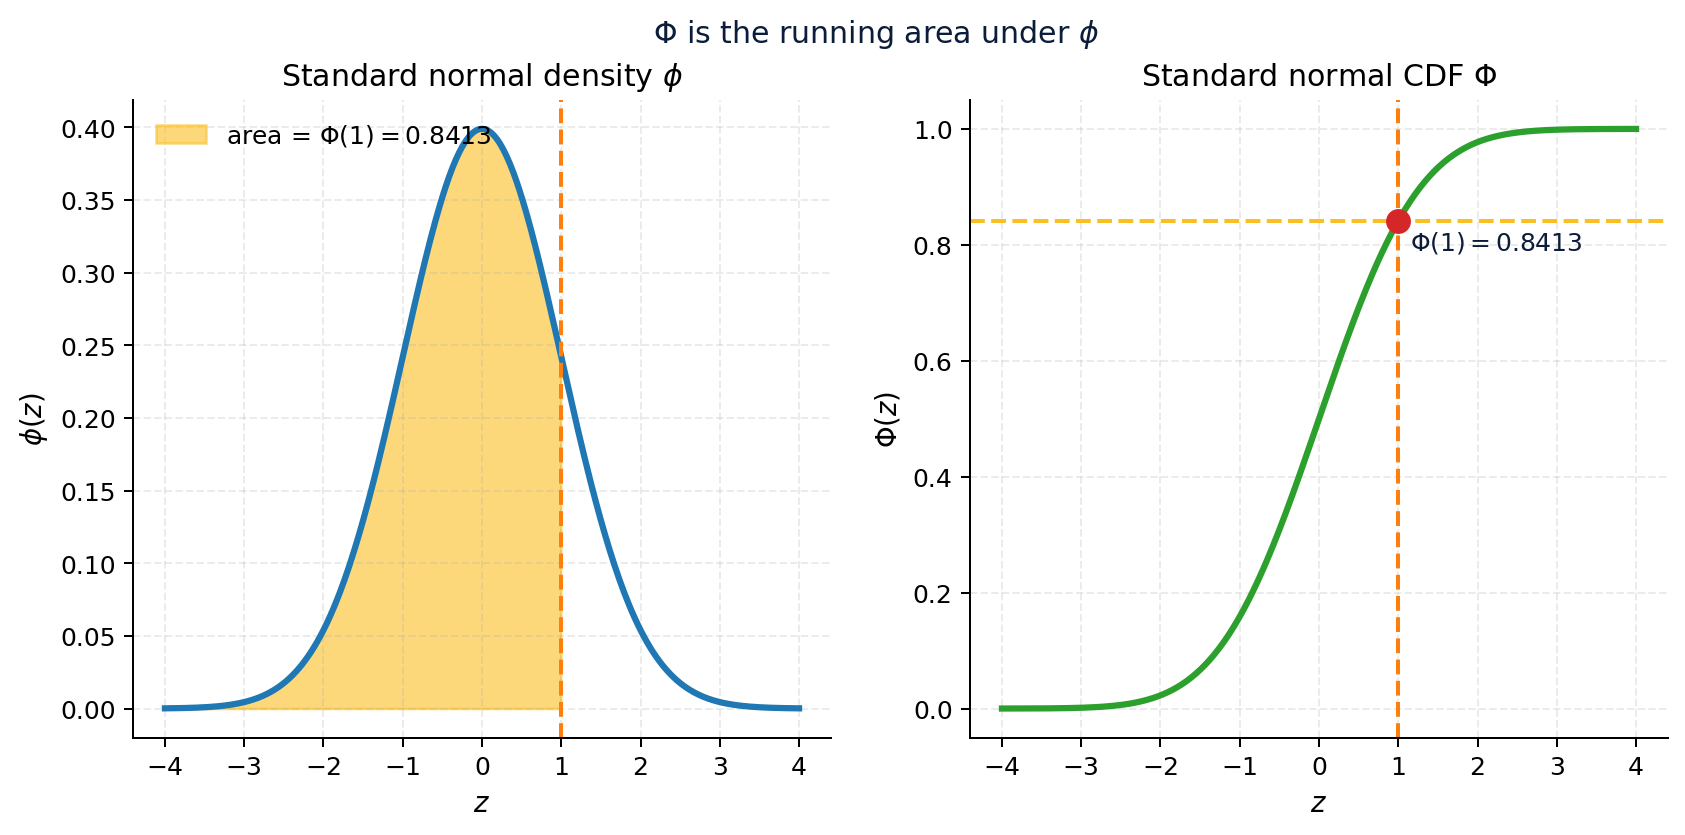
\includegraphics[keepaspectratio]{figures/ch00-phi-and-Phi.png}}
\caption{The standard normal density \(\phi(z)\) on the left and its CDF
\(\Phi(z)\) on the right, with a dashed vertical line at \(z = 1\)
connecting the two. The shaded area under \(\phi\) from \(-\infty\) to
\(1\) equals the height of \(\Phi\) at \(z = 1\), namely \(0.8413\).
\(\Phi\) is just the ``running area'' under the bell.}
\end{figure}

\begin{figure}
\centering
\pandocbounded{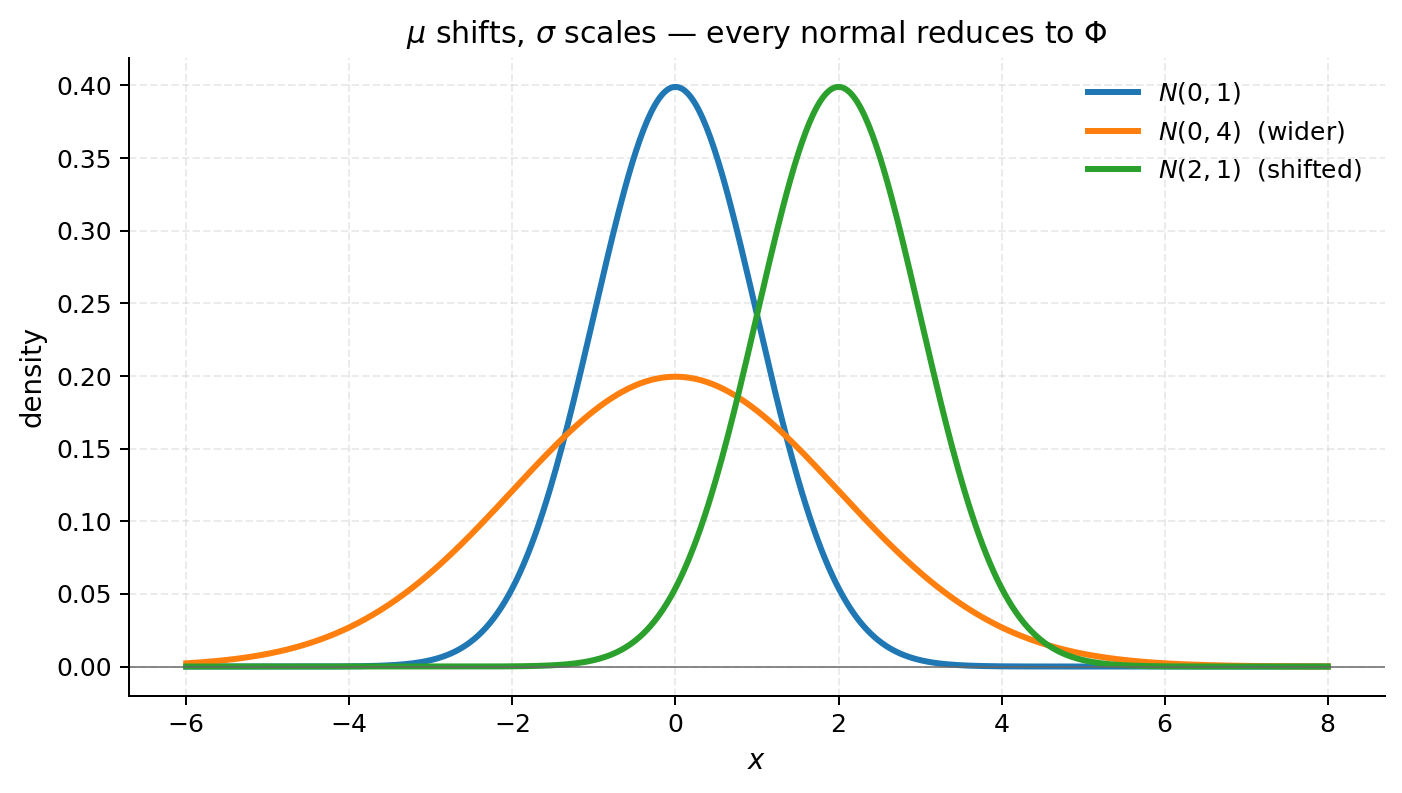
\includegraphics[keepaspectratio]{figures/ch00-three-normals.png}}
\caption{Three normal densities side by side: \(N(0,1)\) in blue,
\(N(0,4)\) in orange (wider), \(N(2,1)\) in green (shifted right).
\(\mu\) shifts; \(\sigma\) scales. Every normal probability reduces by
standardisation to a \(\Phi\) lookup on the blue curve.}
\end{figure}

\subsection{0.9.3 Tables}\label{tables-4}

\textbf{Table 0.11.} Selected \(\Phi\) values with interpretations (full
appendix Table 0.A spans \(z=0\) to \(z=3.49\)).

{\def\LTcaptype{none} % do not increment counter
\begin{table}[H]
\centering
\begin{tabular}{|c|c|l|}
\toprule
\(z\) & \(\Phi(z)\) & Interpretation \\
\midrule



\(0.000\) & \(0.5000\) & symmetric peak \\
\(1.000\) & \(0.8413\) & one-sigma right of mean \\
\(1.645\) & \(0.9500\) & 95th percentile \\
\(1.960\) & \(0.9750\) & two-sided \(95\%\) confidence \\
\(2.326\) & \(0.9900\) & 99th percentile \\
\(2.576\) & \(0.9950\) & two-sided \(99\%\) confidence \\
\(3.090\) & \(0.9990\) & 99.9th percentile \\
\bottomrule
\end{tabular}
\end{table}
}

\subsection{0.9.4 Exercises}\label{exercises-8}

\begin{enumerate}
\def\labelenumi{\arabic{enumi}.}
\tightlist
\item
  \(\mathbb{P}(Z \leq -1.5)\). \textbf{Answer:} \(0.0668\).
\item
  \(X \sim N(50, 10^2)\), \(\mathbb{P}(40 < X < 70)\). \textbf{Answer:}
  \(\Phi(2) - \Phi(-1) = 0.9772 - 0.1587 = 0.8185\).
\item
  \(z\) such that \(\mathbb{P}(|Z| > z) = 0.05\). \textbf{Answer:}
  \(1.96\).
\end{enumerate}

\begin{center}\rule{0.5\linewidth}{0.5pt}\end{center}

\section{§0.10 The Central Limit Theorem (de Moivre--Laplace, with a
Stirling proof
sketch)}\label{the-central-limit-theorem-de-moivrelaplace-with-a-stirling-proof-sketch}

\textbf{Punchline.} Take any independent identically distributed random
variables with finite variance. Add up many of them; subtract the mean;
divide by \(\sigma\sqrt{n}\). As \(n\) grows, the result looks like
\(N(0, 1)\). The \textbf{de Moivre--Laplace} case --- coin tosses --- is
the only one the rest of this book uses, and we give a
\emph{calculus-free} proof sketch below using Stirling's approximation
and an algebraic expansion of a finite product.

\textbf{Intuition.} Each individual flip is small and noisy. Sum many
independent ones and the cancellations smooth out the noise. The
smoothing is so reliable that the limiting shape depends only on the
mean and variance of each piece, \emph{not} on the original
distribution. A sum of fair coin flips and a sum of dice rolls and a sum
of stock-day returns all look like bells once you standardise.
\emph{This is why the binomial pricing sum collapses to a normal CDF in
Chapter 7's Black--Scholes limit.}

\subsection{0.10.1 Definitions and facts}\label{definitions-and-facts-1}

\textbf{Central Limit Theorem (CLT, stated).} Let
\(X_1, X_2, \dots, X_n\) be independent, identically distributed random
variables with mean \(\mu\) and finite variance \(\sigma^2\). Set
\(S_n = X_1 + \dots + X_n\). Then

\[\frac{S_n - n\mu}{\sigma \sqrt{n}} \;\xrightarrow{\text{distribution}}\; N(0, 1) \quad \text{as } n \to \infty.\]

Translation: for large \(n\),

\[\mathbb{P}\!\left(\frac{S_n - n\mu}{\sigma \sqrt{n}} \leq z\right) \;\approx\; \Phi(z).\]

\textbf{De Moivre--Laplace (binomial special case).} If
\(H \sim \mathrm{Bin}(n, p)\), then for large \(n\),

\[\mathbb{P}(H \leq k) \;\approx\; \Phi\!\left(\frac{k + 0.5 - np}{\sqrt{np(1-p)}}\right).\]

The \(+0.5\) is the \emph{continuity correction}: a \(1\)-unit-wide bar
on a histogram, centred at \(k\), extends from \(k - 0.5\) to
\(k + 0.5\); the normal approximation should match by treating the bar
as a strip of width 1.

\textbf{Rule of thumb.} The approximation is good when
\(np(1-p) \geq 10\), i.e., when the binomial is fat enough that several
bars are around the mean.

\subsection{0.10.1a Calculus-free proof sketch (de Moivre--Laplace, fair
coin)}\label{a-calculus-free-proof-sketch-de-moivrelaplace-fair-coin}

We sketch \emph{why} the binomial PMF traces the bell curve, using
nothing beyond Stirling's formula and the algebraic identity
\(\log(1 + u) \approx u - u^2/2\) for small \(u\) (treated as a
polynomial fact about that combination --- no rate-of-change reasoning).

\textbf{Setup.} Let \(H \sim \mathrm{Bin}(n, 1/2)\), so
\(H = X_1 + \dots + X_n\) with \(X_i \in \{0, 1\}\) fair. Mean is
\(n/2\) and variance is \(n/4\), so the standardised count is

\[Z_n \;=\; \frac{H - n/2}{\sqrt{n/4}}.\]

Write \(H = n/2 + j\) where \(j\) is the \emph{signed deviation from the
mean}. Then \(z = 2j/\sqrt{n}\) and consecutive values of \(j\) map to a
\(z\)-spacing \(\Delta z = 2/\sqrt{n}\).

\textbf{Goal.} Show that for \(|j| \ll n\),

\[\mathbb{P}(H = n/2 + j) \;\approx\; \frac{1}{\sqrt{\pi n / 2}} \, e^{-2 j^2 / n}.\]

Once we have this, translation to the \(z\)-scale lands directly on
\(\phi(z)\,\Delta z\).

\begin{center}\rule{0.5\linewidth}{0.5pt}\end{center}

\textbf{Step 1 --- Apply Stirling to the binomial coefficient.} State
Stirling as a fact: for large \(n\),

\[n! \;\approx\; n^n e^{-n} \sqrt{2\pi n}.\]

The PMF at \(H = n/2 + j\) is

\[\mathbb{P}(H = n/2 + j) \;=\; \frac{1}{2^n} \binom{n}{n/2 + j} \;=\; \frac{1}{2^n} \cdot \frac{n!}{(n/2 + j)!\,(n/2 - j)!}.\]

When \(j = 0\), the Stirling-derived peak is (carried over from §0.9)

\[\mathbb{P}(H = n/2) \;=\; \frac{1}{2^n}\binom{n}{n/2} \;\approx\; \frac{1}{\sqrt{\pi n / 2}}.\]

For \(j \neq 0\), peel the centre coefficient off as a \emph{ratio of
factorials} --- this is pure algebra:

\[\binom{n}{n/2 + j} \;=\; \binom{n}{n/2} \cdot \prod_{i=1}^{j} \frac{n/2 - i + 1}{n/2 + i}.\]

(One factor for each unit of deviation from the centre --- the numerator
pulls down from \(n/2\), the denominator pushes up.) Dividing by
\(2^n\),

\[\mathbb{P}(H = n/2 + j) \;\approx\; \frac{1}{\sqrt{\pi n / 2}} \cdot \prod_{i=1}^{j} \frac{n/2 - i + 1}{n/2 + i}.\]

No calculus has been used --- only Stirling and factorial telescoping.

\begin{center}\rule{0.5\linewidth}{0.5pt}\end{center}

\textbf{Step 2 --- Algebraic expansion of the product.} Take logarithms
to turn the product into a sum:

\[\log \prod_{i=1}^{j} \frac{n/2 - i + 1}{n/2 + i} \;=\; \sum_{i=1}^{j} \log\!\left(\frac{n/2 - i + 1}{n/2 + i}\right).\]

Factor \(n/2\) out of numerator and denominator inside each term:

\[\frac{n/2 - i + 1}{n/2 + i} \;=\; \frac{1 - (i - 1)/(n/2)}{1 + i/(n/2)} \;=\; \frac{1 - 2(i-1)/n}{1 + 2i/n}.\]

For \(i \ll n/2\), both correction terms are small. Use the polynomial
identity (state as a fact)

\[\log(1 + u) \;\approx\; u - \tfrac{1}{2} u^2 \qquad \text{for small } u,\]

applied to numerator and denominator separately:

\[
\begin{aligned}
\log\!\left(1 - \tfrac{2(i-1)}{n}\right) &\;\approx\; -\tfrac{2(i-1)}{n} - \tfrac{1}{2}\!\left(\tfrac{2(i-1)}{n}\right)^2, \\
\log\!\left(1 + \tfrac{2i}{n}\right) &\;\approx\; \tfrac{2i}{n} - \tfrac{1}{2}\!\left(\tfrac{2i}{n}\right)^2.
\end{aligned}
\]

Subtract:

\[\log\!\left(\frac{n/2 - i + 1}{n/2 + i}\right) \;\approx\; -\frac{2(i - 1)}{n} - \frac{2i}{n} \;+\; (\text{quadratic-in-}i/n \text{ terms that vanish like } 1/n).\]

The leading piece is \(-(4i - 2)/n\). Sum over \(i = 1, 2, \dots, j\):

\[
\begin{aligned}
\sum_{i=1}^{j} -\frac{4i - 2}{n}
&\;=\; -\frac{4 \cdot j(j+1)/2 - 2j}{n} \\
&\;=\; -\frac{2j^2 + 2j - 2j}{n} \;=\; -\frac{2 j^2}{n}.
\end{aligned}
\]

Used here: \(\sum_{i=1}^{j} i = j(j+1)/2\) (a triangular-number identity
from §0.3). The \(O(1/n)\) corrections drop out for
\(|j| \ll \sqrt{n}\).

So

\[\log \prod_{i=1}^{j} \frac{n/2 - i + 1}{n/2 + i} \;\approx\; -\frac{2 j^2}{n}, \qquad \prod \;\approx\; e^{-2 j^2 / n}.\]

No integrals, no derivatives --- just Stirling, the polynomial identity
for \(\log(1+u)\), and the triangular-number sum.

\begin{center}\rule{0.5\linewidth}{0.5pt}\end{center}

\textbf{Step 3 --- Combine and translate to the standardised scale.}
Plugging the product back into Step 1,

\[\mathbb{P}(H = n/2 + j) \;\approx\; \frac{1}{\sqrt{\pi n / 2}} \, e^{-2 j^2 / n}.\]

Now set \(z = 2j / \sqrt{n}\). Then \(2 j^2 / n = z^2/2\), and
consecutive integer values of \(j\) have \(z\)-spacing
\(\Delta z = 2/\sqrt{n}\). So

\[\mathbb{P}(Z_n = z) \;=\; \mathbb{P}(H = n/2 + j) \;\approx\; \frac{1}{\sqrt{\pi n / 2}} \, e^{-z^2/2}.\]

Substitute
\(\sqrt{\pi n/2} = \sqrt{2\pi} \cdot \sqrt{n}/2 = \sqrt{2\pi}/\Delta z\):

\[\mathbb{P}(Z_n \in [z, z + \Delta z]) \;\approx\; \frac{1}{\sqrt{2\pi}} \, e^{-z^2/2} \, \Delta z \;=\; \phi(z)\,\Delta z.\]

\textbf{The big reveal.} The standardised binomial PMF, viewed as a
Riemann sum on the \(z\)-axis with spacing \(\Delta z\), traces
\emph{exactly} the standard normal density \(\phi(z)\). Summing those
bars from \(-\infty\) to \(z\) gives the running total \(\Phi(z)\), the
tabulated function we already met in §0.9. That is de Moivre--Laplace.

\textbf{Worked numerical check for \(n = 100\)} (so \(n/2 = 50\),
\(\sqrt{n/4} = 5\)). Compare the Stirling-derived approximation
\(\frac{1}{\sqrt{\pi n/2}} e^{-2 j^2 / n}\) with the exact binomial PMF.

{\def\LTcaptype{none} % do not increment counter
\begin{table}[H]
\centering
\begin{tabular}{|r|r|r|r|r|}
\toprule
\(j\) & \(z = 2j/\sqrt{n}\) & Exact \(\mathbb{P}(H = 50 + j)\) & Approx \(\frac{1}{\sqrt{50\pi}}\, e^{-j^2/50}\) & Rel. error \\
\midrule



\(0\) & \(0.0\) & \(0.07959\) & \(0.07979\) & \(0.25\%\) \\
\(5\) & \(1.0\) & \(0.04847\) & \(0.04839\) & \(0.17\%\) \\
\(10\) & \(2.0\) & \(0.01084\) & \(0.01080\) & \(0.42\%\) \\
\(20\) & \(4.0\) & \(2.32 \times 10^{-5}\) & \(2.68 \times 10^{-5}\) &
\(15.5\%\) \\
\bottomrule
\end{tabular}
\end{table}
}

At \(j = 5, 10\) the agreement is well under half a percent; out at
\(j = 20\) (four standard deviations from the mean) the error widens
visibly because the dropped \(O(j^4/n^3)\) tail terms accumulate where
\(j\) is no longer small relative to \(\sqrt{n}\). \emph{This is
precisely what we promised:} the approximation is sharp in the bulk,
soft in the deep tails --- and the bulk is where every Chapter-7 strike
sits.

\begin{center}\rule{0.5\linewidth}{0.5pt}\end{center}

\textbf{Generalisation to non-symmetric \(p\) (stated).} The same
argument with \(p \neq 1/2\) runs through. Stirling gives

\[\binom{n}{k} p^k (1-p)^{n-k} \;\approx\; \frac{1}{\sqrt{2\pi n p (1-p)}} \, e^{-(k - np)^2 / (2 n p (1-p))},\]

so the standardised binomial \((H - np)/\sqrt{np(1-p)}\) approaches
\(N(0,1)\). Only the \emph{centre} and the \emph{spacing} change; the
product expansion picks up an asymmetric bias term that still sums to a
single quadratic in the deviation. We will not re-do the algebra --- the
symmetric case carries all the conceptual weight.

\textbf{Generalisation to non-Bernoulli (CLT proper).} Replace each fair
flip by \emph{any} random variable with mean \(\mu\) and finite variance
\(\sigma^2\), summed independently. The same Riemann-sum/bell-curve
phenomenon emerges, by an argument that --- at full generality --- needs
more machinery (characteristic functions or moment-generating functions)
than we have. We adopt it as a \emph{fact}. The de Moivre--Laplace case
proved above is the only one Chapters 1--7 actually use.

\subsection{0.10.2 Examples}\label{examples-9}

\begin{figure}
\centering
\pandocbounded{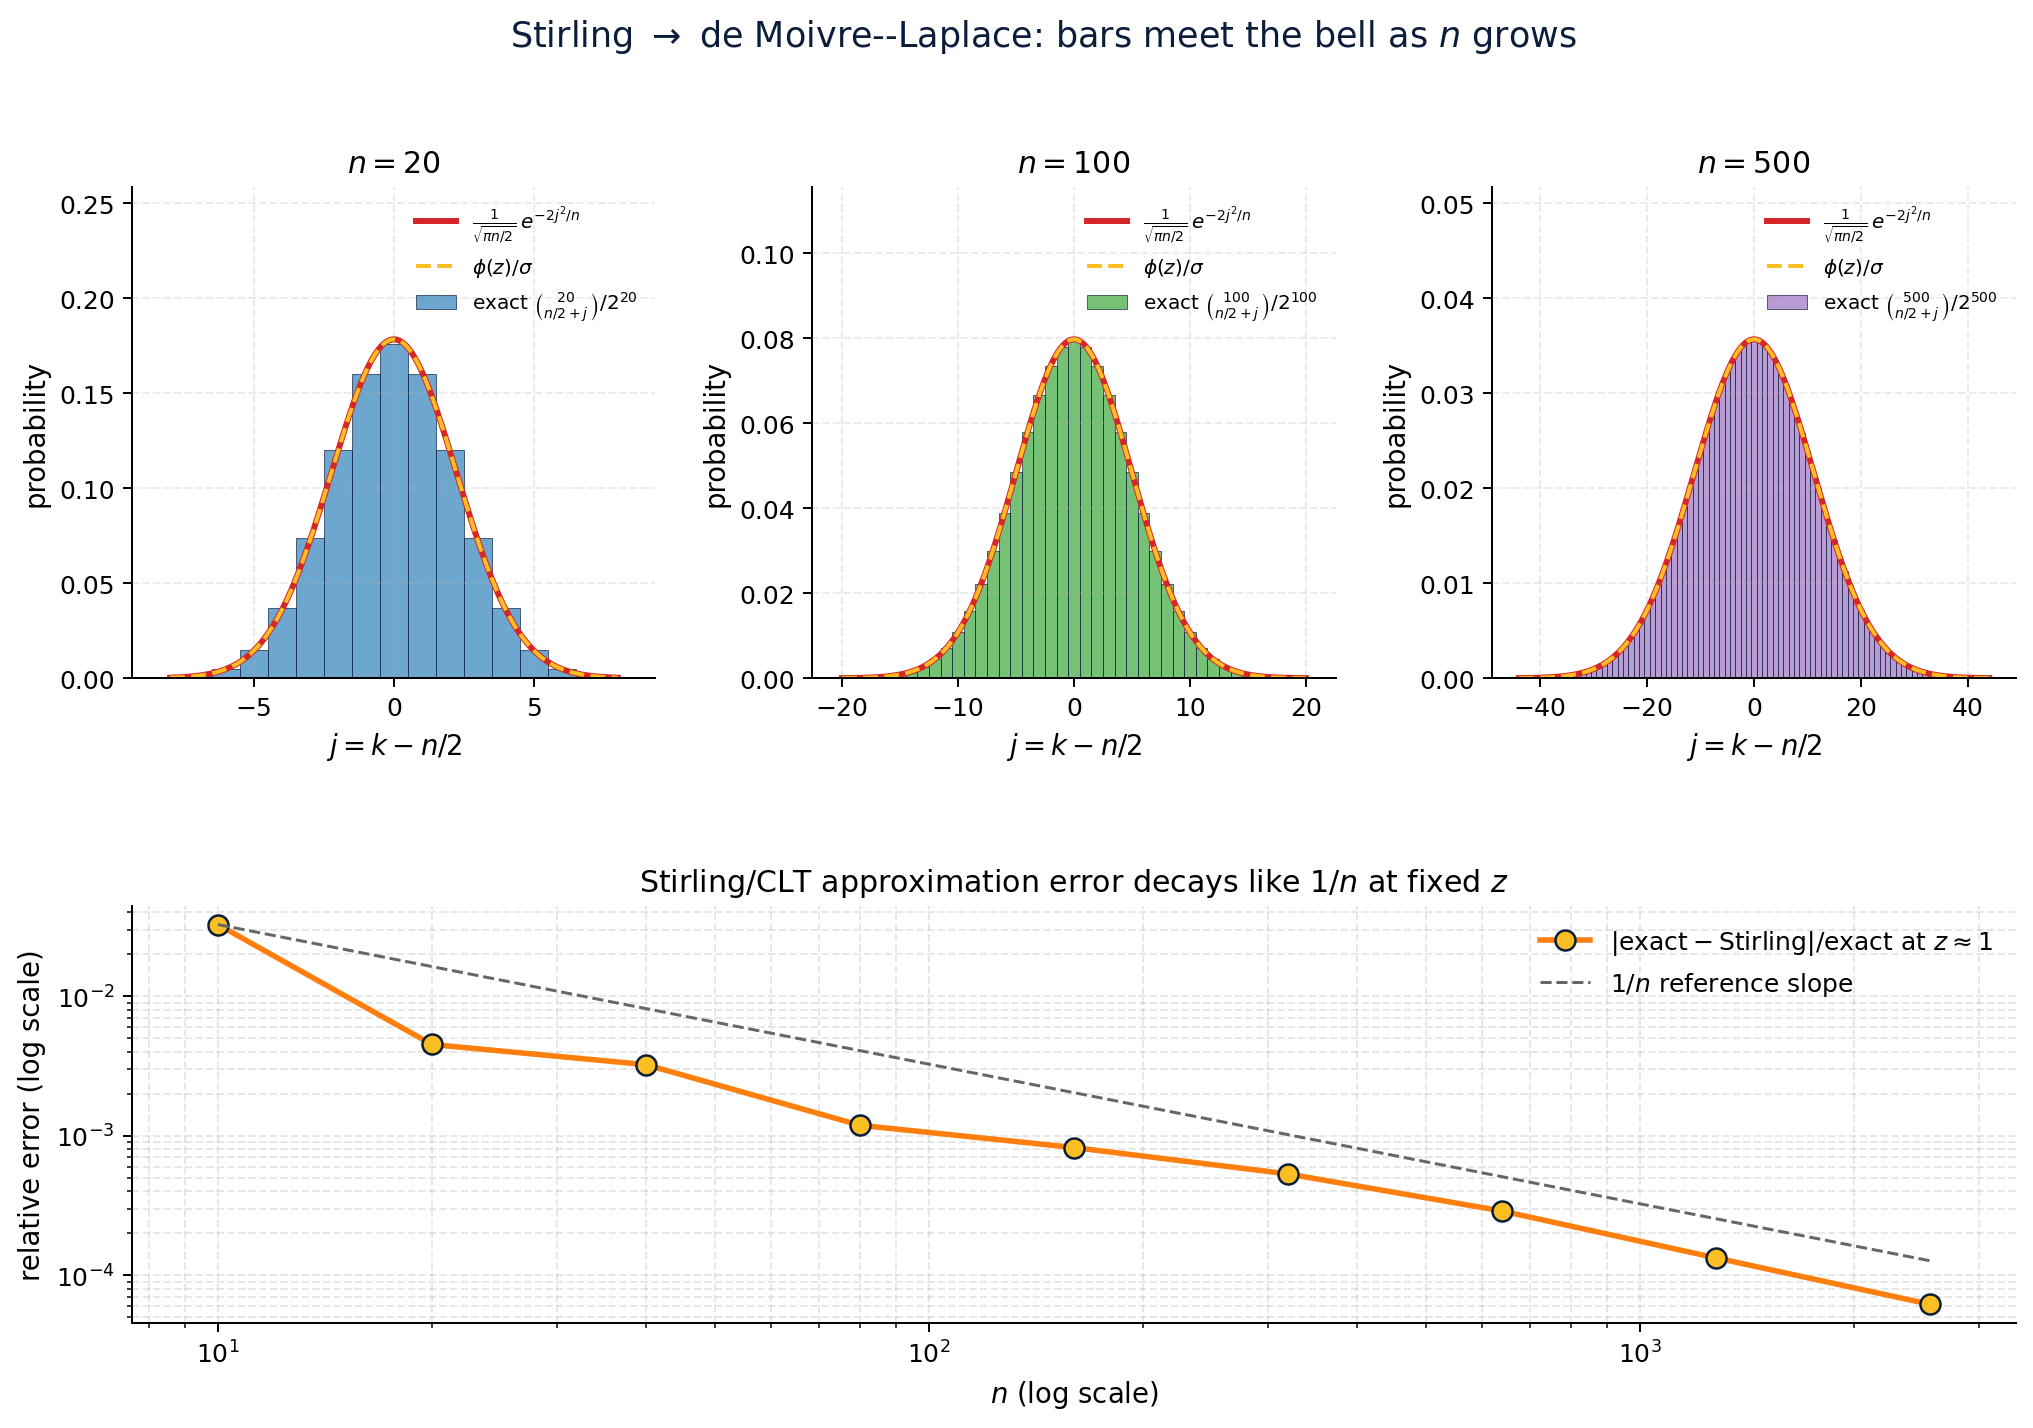
\includegraphics[keepaspectratio]{figures/ch00-stirling-clt-proof.png}}
\caption{Four-panel storyboard of the Stirling/CLT proof sketch. Top
row: exact binomial PMF bars \(\binom{n}{n/2 + j}/2^n\) versus the
Stirling approximation \(\frac{1}{\sqrt{\pi n/2}}\,e^{-2 j^2/n}\) (red
curve) at \(n = 20, 100, 500\). Bottom row: standardised version with
the limiting \(\phi(z)\) traced as \(n\) grows; log-scale plot of
relative error vs \(n\) at fixed deviation ratio \(j/\sqrt{n}\).}
\end{figure}

\textbf{Example 0.10.X (Stirling on \(10!\)).} Exact
\(10! = 3{,}628{,}800\). Stirling:
\(10^{10} e^{-10} \sqrt{20\pi} = 10^{10} \cdot 4.53999 \times 10^{-5} \cdot 7.92665 \approx 3{,}598{,}696\).
Relative error
\(\approx |3{,}628{,}800 - 3{,}598{,}696| / 3{,}628{,}800 \approx 0.83\%\).
Stirling is already accurate below the 1\%-level at \(n = 10\); by
\(n = 100\) it sits below 0.1\%.

\textbf{Example 0.10.Y (Bin\((16, 1/2)\) vs normal at \(j = 2\)).} Mean
\(8\), \(\sigma = 2\). Compare exact PMF at \(H = 10\) (\(j = 2\)) with
the Stirling approximation
\(\frac{1}{\sqrt{8\pi}}\,e^{-2 \cdot 4/16} = \frac{1}{\sqrt{8\pi}}\,e^{-0.5}\).

\begin{itemize}
\tightlist
\item
  Exact: \(\binom{16}{10}/2^{16} = 8008/65536 = 0.12219\).
\item
  Approx:
  \(1/\sqrt{8\pi} \cdot e^{-0.5} = 0.19947 \cdot 0.60653 = 0.12099\).
\item
  Relative error: \(0.98\%\).
\end{itemize}

Even at \(n = 16\) --- a \emph{small} sample size by the standards of
CLT --- the Stirling argument already agrees to within one percent. By
Chapter 7's \(n\)-period binomial tree (with \(n \gg 100\) steps to
expiry), the agreement is well inside the rounding noise of our \(\Phi\)
table.

\textbf{Example 0.10.Z (CLT on a dice sum).} Roll a fair six-sided die
\(n = 30\) times; let \(S = X_1 + \dots + X_{30}\). Per die:
\(\mu = 3.5\), \(\sigma^2 = 35/12 \approx 2.917\), \(\sigma = 1.708\).
Sum: \(\mu_S = 105\),
\(\sigma_S = \sqrt{30 \cdot 35/12} = \sqrt{87.5} \approx 9.354\).

Find \(\mathbb{P}(S \geq 120)\) via CLT with continuity correction:

\[
\begin{aligned}
\mathbb{P}(S \geq 120)
&\;=\; \mathbb{P}\!\left(\frac{S - 105}{9.354} \geq \frac{119.5 - 105}{9.354}\right) \\
&\;\approx\; 1 - \Phi(1.550) \;=\; 1 - 0.9394 \;=\; 0.0606.
\end{aligned}
\]

About \(6\%\) chance the 30-die sum exceeds 120. (The dice outcome
distribution is \emph{not} normal --- it is a discrete uniform on
\(\{1, \dots, 6\}\). The CLT does not care: only the per-die mean and
variance enter the answer.)

\textbf{Example 0.10.1 (small case, fair).} Bin\((100, 0.5)\). Mean
\(= 50\), \(\sigma = 5\). Find \(\mathbb{P}(H \leq 55)\).

CLT approximation: \(\Phi((55 + 0.5 - 50)/5) = \Phi(1.1) = 0.8643\).

Exact (compute the binomial sum): \(0.8644\).

Agreement to three decimal places.

\textbf{Example 0.10.2 (medium case, fair).} Bin\((400, 0.5)\). Mean
\(200\), \(\sigma = 10\).
\(\mathbb{P}(H \geq 220) = 1 - \Phi((220 - 0.5 - 200)/10) = 1 - \Phi(1.95) = 1 - 0.9744 = 0.0256\).

Exact: \(0.0282\). Slight underestimate; the continuity correction has
improved the agreement vs no correction.

\textbf{Example 0.10.3 (sum of 100 fair dice).} \(\mu = 3.5\),
\(\sigma^2 = 35/12\) per die. Sum of 100: \(\mu_{S} = 350\),
\(\sigma_{S}^2 = 100 \cdot 35/12 = 291.67\), \(\sigma_S = 17.08\).

\(\mathbb{P}(\text{sum} \leq 380) \approx \Phi((380 - 350)/17.08) = \Phi(1.756) = 0.9605\).

\textbf{Example 0.10.4 (foreshadowing Black--Scholes).} \(u = 1.10\),
\(d = 0.90\), \(n = 100\), \(\tilde p = 0.5\). The terminal log return
is \(\ln(S_n / S_0) = H \ln u + (n - H) \ln d\) where
\(H \sim \mathrm{Bin}(n, \tilde p)\).

\begin{itemize}
\tightlist
\item
  Per flip:
  \(\mathbb{E}[\ln G_i] = 0.5 (\ln 1.10 + \ln 0.90) = 0.5(0.09531 - 0.10536) = -0.005025\).
\item
  Per flip:
  \(\mathrm{Var}(\ln G_i) = 0.5 (\ln 1.10)^2 + 0.5 (\ln 0.90)^2 - (-0.005025)^2 \approx 0.01010\).
\item
  Over 100 flips: mean \(= -0.5025\), variance \(= 1.010\),
  \(\sigma = 1.005\).
\end{itemize}

By CLT, \(\ln(S_{100}/S_0) \approx N(-0.5025, 1.010)\). The probability
the stock ends \emph{above} its start,
\(\mathbb{P}(S_{100} > S_0) = \mathbb{P}(\ln(S_{100}/S_0) > 0)\), is

\[1 - \Phi\!\left(\frac{0 - (-0.5025)}{1.005}\right) = 1 - \Phi(0.500) = 1 - 0.6915 = 0.3085.\]

About \(31\%\) chance the stock ends up after 100 fair flips between
\(\pm 10\%\) moves. The downward bias comes from
\(\ln 1.1 + \ln 0.9 < 0\) --- the symmetry trap from §0.1 in full
effect.

\textbf{Example 0.10.5 (continuity-correction comparison).} With
\(\sigma = \sqrt{n/4}\), compare exact
\(\mathbb{P}(H \leq \lfloor n/2 + \sigma \rfloor)\) against the normal
approximation with and without a continuity correction.

{\def\LTcaptype{none} % do not increment counter
\begin{table}[H]
\centering
\begin{tabular}{|c|c|c|c|c|}
\toprule
\(n\) & threshold \(\lfloor n/2{+}\sigma\rfloor\) & exact & normal & normal + cc \\
\midrule



\(10\) & \(6\) & \(0.8281\) & \(0.8413\) & \(0.8531\) \\
\(40\) & \(23\) & \(0.8461\) & \(0.8413\) & \(0.8534\) \\
\(100\) & \(55\) & \(0.8644\) & \(0.8413\) & \(0.8643\) \\
\(400\) & \(210\) & \(0.8462\) & \(0.8413\) & \(0.8531\) \\
\bottomrule
\end{tabular}
\end{table}
}

The plain-normal column always evaluates at \(z = 1\) (so the same
\(0.8413\)). The continuity-corrected column uses
\(z = (\lfloor n/2+\sigma\rfloor + 0.5 - n/2)/\sigma\) --- slightly
above \(1\) when the floor truncates.

\textbf{Example 0.10.6 (CLT-quality of fit visual).} Maximum PMF error
of Bin\((n, 0.5)\) versus the matching normal density, for
\(n = 10, 40, 160, 640\).

{\def\LTcaptype{none} % do not increment counter
\begin{table}[H]
\centering
\begin{tabular}{|c|c|}
\toprule
\(n\) & max error \\
\midrule



\(10\) & \(0.00700\) \\
\(40\) & \(0.00170\) \\
\(160\) & \(0.00043\) \\
\(640\) & \(0.00011\) \\
\bottomrule
\end{tabular}
\end{table}
}

The ``max error'' column is the maximum over \(k\) of
\(\lvert\mathbb{P}(H=k) - \phi((k-\mu)/\sigma)/\sigma\rvert\) where
\(\mu = n/2\) and \(\sigma = \sqrt{n/4}\).

Each row reduces the error by about a factor of 4 --- this is the
\emph{local} CLT rate \(O(1/n)\) for the PMF (Berry--Esseen
\(O(1/\sqrt n)\) controls the CDF instead).

\begin{figure}
\centering
\pandocbounded{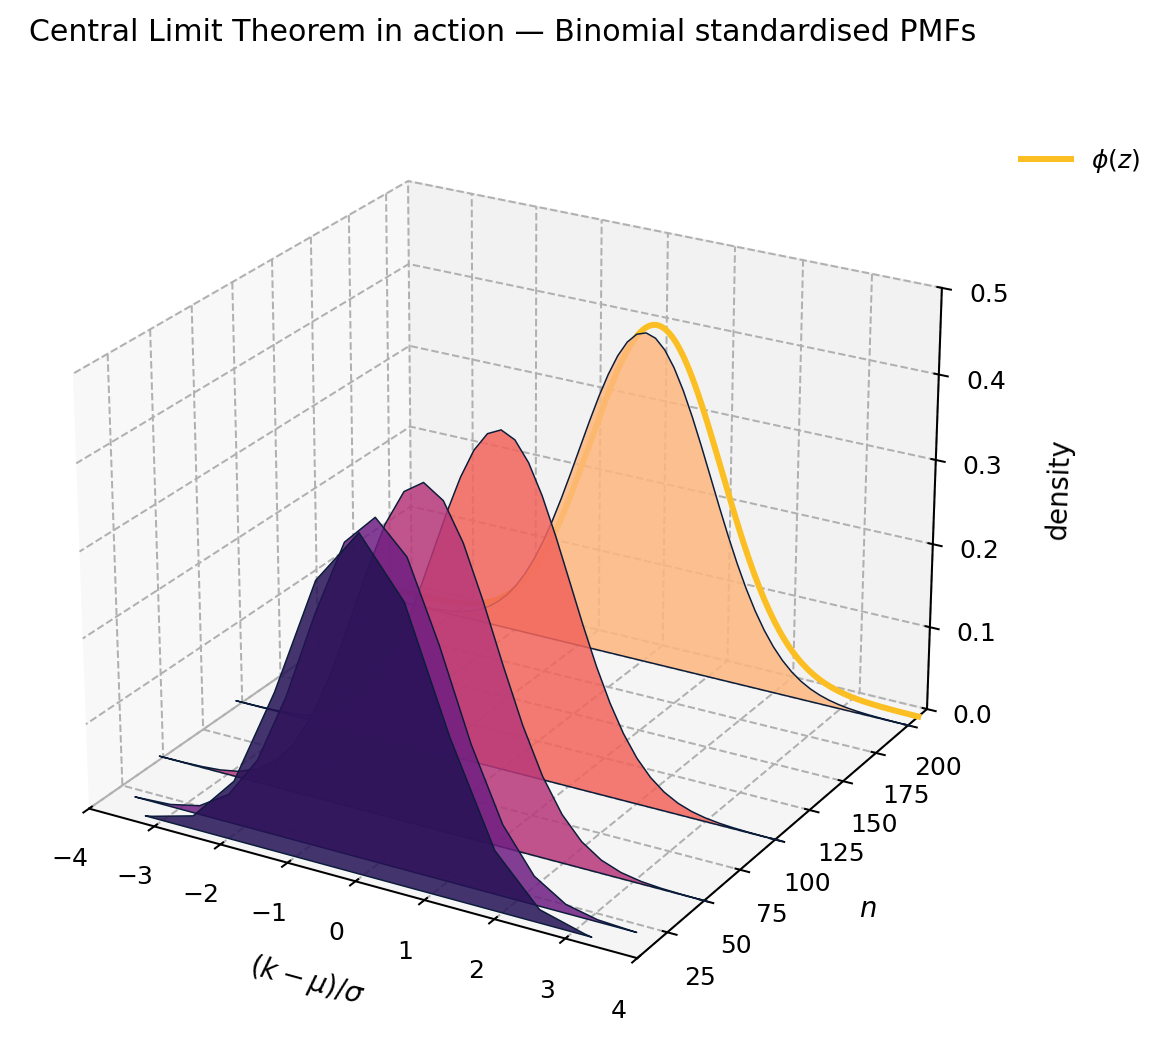
\includegraphics[keepaspectratio]{figures/ch00-clt-ridge-3d.png}}
\caption{3-D ridge surface plot of Bin\((n, 0.5)\) standardised PMFs for
\(n = 10, 20, 50, 100, 200\). The far-end ridge is the limiting normal
curve. Each ridge is rescaled so the \(x\)-axis is \((k - \mu)/\sigma\);
convergence is the visible ``smoothing'' as you walk along the \(n\)
axis.}
\end{figure}

\begin{figure}
\centering
\pandocbounded{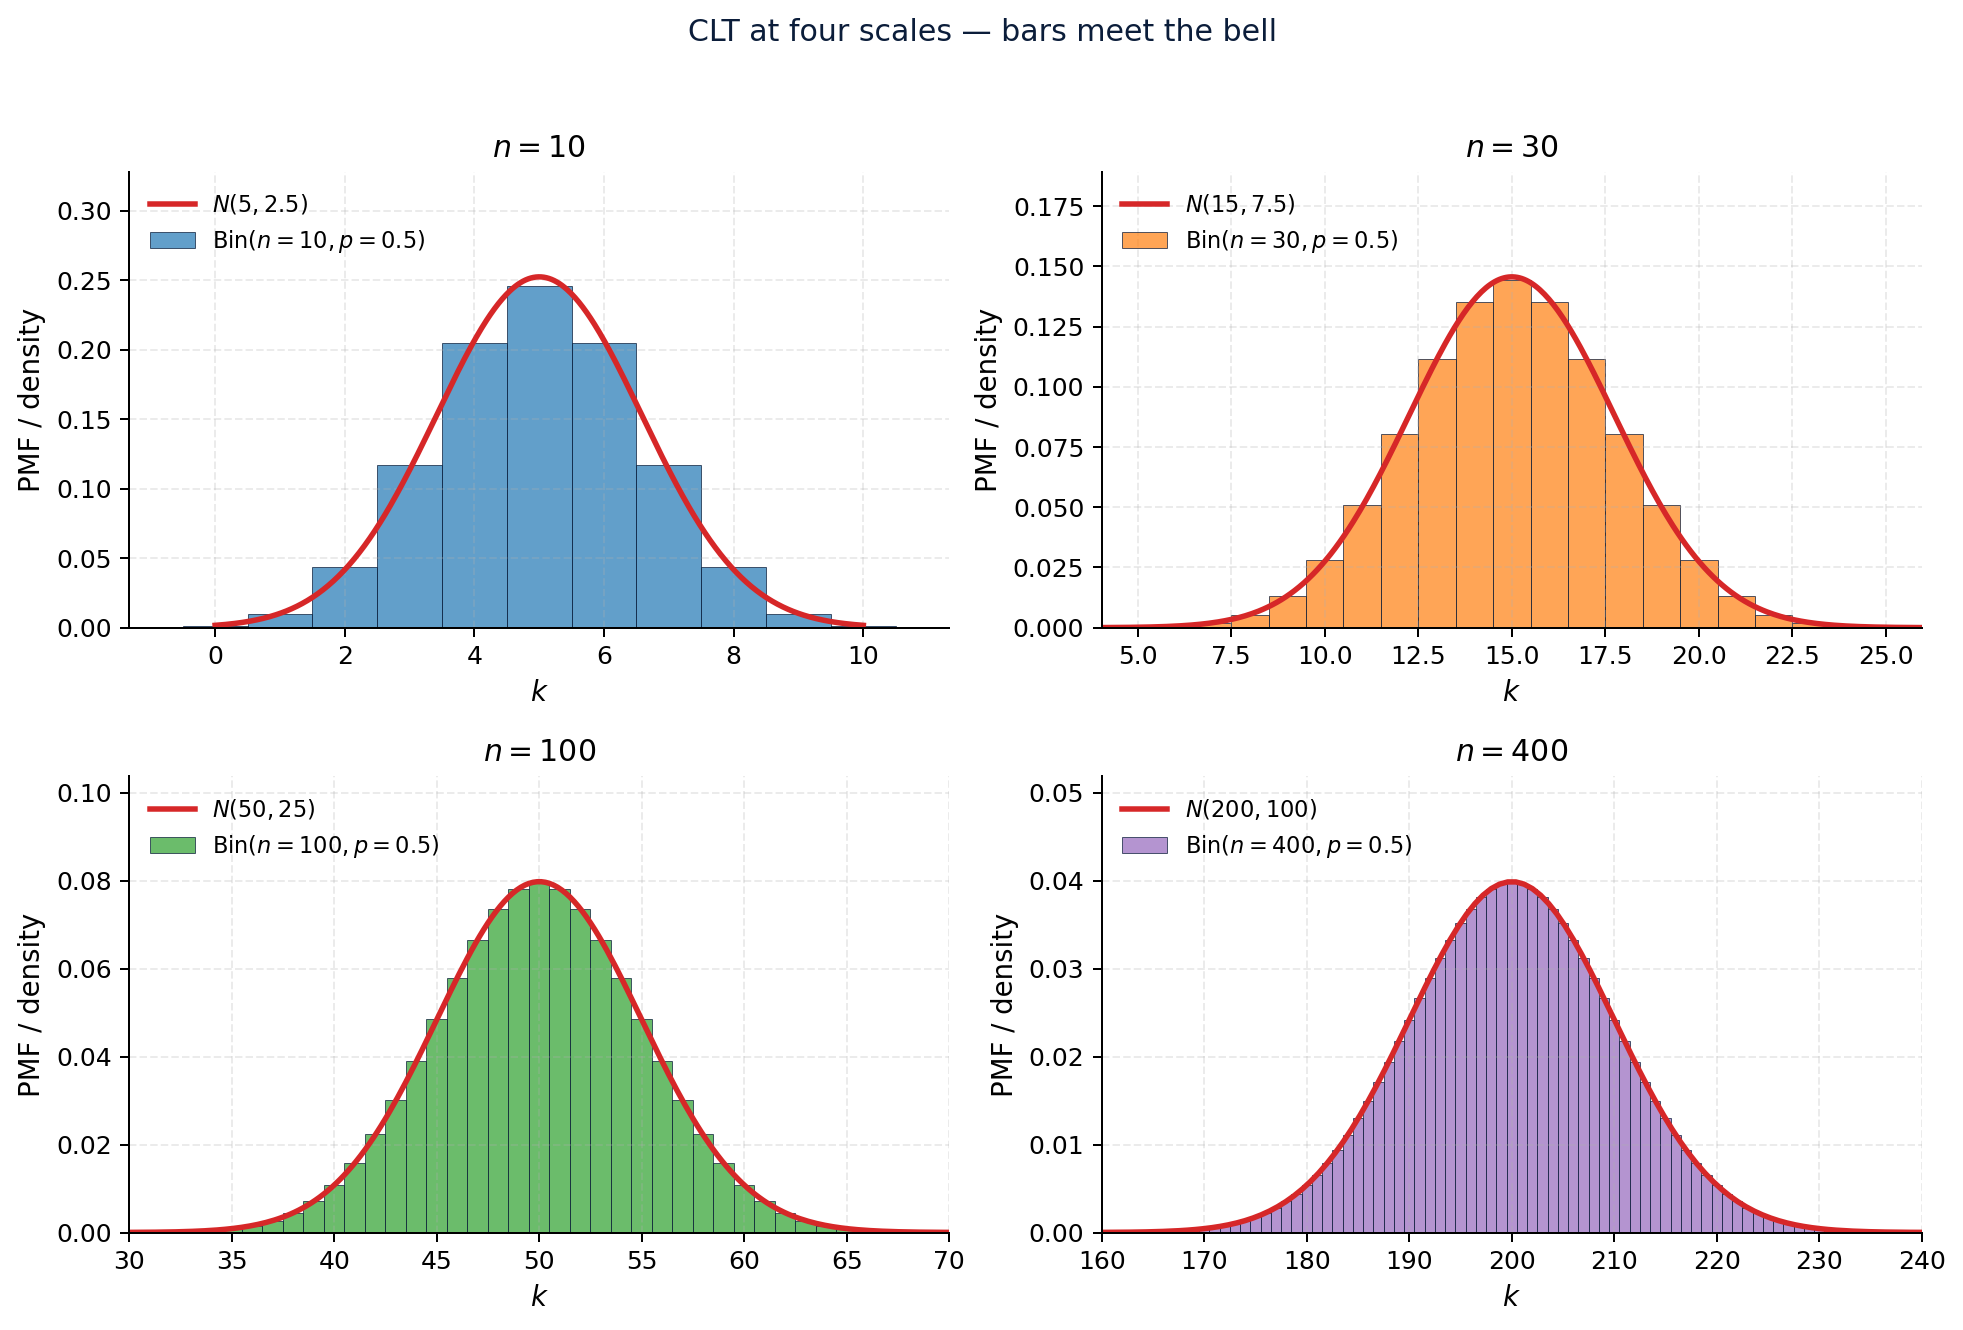
\includegraphics[keepaspectratio]{figures/ch00-clt-4-panels.png}}
\caption{Four-panel grid: bar PMFs of Bin\((n, 0.5)\) for
\(n = 10, 30, 100, 400\), overlaid with the matching normal density
(rescaled to PMF units). Each panel demonstrates the convergence at a
different scale.}
\end{figure}

\subsection{0.10.3 Tables}\label{tables-5}

\textbf{Table 0.12.} Binomial vs normal:
\(\mathbb{P}(H \leq \lfloor n/2 + \sigma\rfloor)\) for symmetric
Bin\((n, 0.5)\) (\(\sigma = \sqrt{n/4}\)), with continuity correction.

{\def\LTcaptype{none} % do not increment counter
\begin{table}[H]
\centering
\begin{tabular}{|r|r|r|r|}
\toprule
\(n\) & Exact & Normal (CC) & Abs. error \\
\midrule



\(\phantom{000}10\) & \(0.8281\) & \(0.8413\) & \(0.0132\) \\
\(\phantom{000}40\) & \(0.8420\) & \(0.8413\) & \(0.0007\) \\
\(\phantom{00}100\) & \(0.8553\) & \(0.8413\) & \(0.0140\) \\
\(\phantom{00}400\) & \(0.8400\) & \(0.8413\) & \(0.0013\) \\
\(1600\) & \(0.8423\) & \(0.8413\) & \(0.0010\) \\
\bottomrule
\end{tabular}
\end{table}
}

Error stays small once \(n \geq 40\) or so --- the CLT is reliable for
the kinds of sample sizes we will use in Chapter 7.

\subsection{0.10.4 Exercises}\label{exercises-9}

\begin{enumerate}
\def\labelenumi{\arabic{enumi}.}
\tightlist
\item
  Bin\((64, 0.5)\), \(\mathbb{P}(H \geq 40)\) via CLT with continuity
  correction. \textbf{Answer:}
  \(1 - \Phi((39.5 - 32)/4) = 1 - \Phi(1.875) = 0.0304\).
\item
  Sum of 50 Bernoulli\((0.3)\), \(\mathbb{P}(\text{sum} \leq 20)\) via
  CLT. \textbf{Answer:}
  \(\Phi((20.5 - 15)/\sqrt{50 \cdot 0.21}) = \Phi(1.697) = 0.9551\).
\item
  What will \(\sigma \sqrt n\) become in the Black--Scholes formula?
  \textbf{Answer:} The ``\(\sigma \sqrt T\)'' factor --- volatility
  times the square root of time-to-maturity. The CLT scaling of standard
  deviations of sums is \emph{the} reason BS prices scale with
  \(\sigma \sqrt T\).
\end{enumerate}

\begin{center}\rule{0.5\linewidth}{0.5pt}\end{center}

\section{§0.11 Solving 2×2 Linear Systems (Replication
Prep)}\label{solving-22-linear-systems-replication-prep}

\textbf{Punchline.} Two equations, two unknowns. Subtract one from the
other to eliminate one variable. This is \emph{literally} Chapter 1's
replication math --- match the option payoff in two states by holding
\(\Delta\) shares and \(B\) dollars in the bond.

\textbf{Intuition.} In a one-period binomial model the stock has two
possible final values, \(S_u\) and \(S_d\). A derivative has two
corresponding final payoffs, \(V_u\) and \(V_d\). We try to
\emph{replicate} the derivative with a portfolio of stock and bond ---
say, \(\Delta\) shares plus \(B\) dollars in the money market. The
portfolio's value in each state must match the derivative's payoff. That
gives us two linear equations in two unknowns. Solve them.

\subsection{0.11.1 Definitions and method}\label{definitions-and-method}

A \(2 \times 2\) linear system:

\[\begin{cases} a\,x + b\,y = p \\ c\,x + d\,y = q \end{cases}\]

has the unique solution (when \(\det = ad - bc \neq 0\)):

\[x = \frac{p d - b q}{a d - b c}, \qquad y = \frac{a q - c p}{a d - b c}.\]

This is Cramer's rule. Equivalently, eliminate \(y\) by computing
\(d \cdot (\text{eq 1}) - b \cdot (\text{eq 2})\).

\subsection{0.11.2 Examples}\label{examples-10}

\textbf{Example 0.11.1 (Toy call).} \(S_0 = 4\), \(u = 2\), \(d = 1/2\),
\(r = 1/4\), call strike \(K = 5\).

\begin{itemize}
\tightlist
\item
  \(S_1 \in \{8, 2\}\). Call payoff: \(V_1(H) = (8 - 5)^+ = 3\),
  \(V_1(T) = (2 - 5)^+ = 0\).
\item
  Replicating portfolio: \(\Delta\) shares + \(B\) dollars in bond
  (growing at rate \(r\)).
\item
  System:
\end{itemize}

\[\begin{cases} \Delta \cdot 8 + B \cdot (1 + 1/4) = 3 \\ \Delta \cdot 2 + B \cdot (1 + 1/4) = 0 \end{cases}\]

Subtract: \(6\Delta = 3\), so \(\Delta = 1/2\). Substitute into the
second: \(1 + (5/4)B = 0\), so \(B = -4/5\).

Replicating portfolio value at time 0:
\(\Delta \cdot S_0 + B = (1/2)(4) + (-4/5) = 2 - 0.8 = 1.20\).

So the no-arbitrage price of this call is \(\$1.20\). We will redo this
in Chapter 1 with full justification.

\textbf{Example 0.11.2 (realistic call).} \(S_0 = 100\), \(u = 1.10\),
\(d = 0.90\), \(r = 0.02\), call strike \(K = 100\).

\begin{itemize}
\tightlist
\item
  \(V_1(H) = 10\), \(V_1(T) = 0\).
\item
  System: \(\Delta \cdot 110 + 1.02 B = 10\),
  \(\Delta \cdot 90 + 1.02 B = 0\).
\item
  Subtract: \(20 \Delta = 10\), \(\Delta = 0.5\). From second:
  \(1.02 B = -45\), \(B = -44.118\).
\item
  Time-0 cost: \((0.5)(100) - 44.118 = 5.882\).
\end{itemize}

Price of this realistic call: \(\$5.88\).

\textbf{Example 0.11.3 (Toy put, \(K = 5\)).} Payoffs:
\(V_1(H) = (5 - 8)^+ = 0\), \(V_1(T) = (5 - 2)^+ = 3\).

\begin{itemize}
\tightlist
\item
  System: \(\Delta \cdot 8 + (5/4) B = 0\),
  \(\Delta \cdot 2 + (5/4) B = 3\).
\item
  Subtract: \(6 \Delta = -3\), \(\Delta = -1/2\). Substitute:
  \(-1 + (5/4) B = 3\), \(B = 16/5\).
\item
  Time-0 cost: \((-1/2)(4) + 16/5 = -2 + 3.2 = 1.20\).
\end{itemize}

The put is also worth \(\$1.20\) on the toy --- same as the call.
(Aside: this is \emph{not} by accident; put--call parity at this strike
and rate forces them equal because \(K = S_0(1 + r) = 5\) exactly.)

\textbf{Example 0.11.4 (the degenerate case).} If \(u = d\), the
determinant \(ad - bc\) becomes \(u(1+r) - u(1+r) = 0\). The two
equations describe the same line; either there is no solution
(inconsistent) or infinitely many. Economically: a stock that has the
same price in both ``outcomes'' has no randomness, so no derivative on
it can have a well-defined price either --- there is nothing to insure
against.

\textbf{Example 0.11.5 (a random non-option payoff).} Same Toy. Payoff
at expiry: \(V_1(H) = 5\), \(V_1(T) = -2\) (a contract that pays you 5
if the stock goes up, costs you 2 if it goes down). System:
\(8 \Delta + (5/4) B = 5\), \(2 \Delta + (5/4) B = -2\). Subtract:
\(6\Delta = 7\), \(\Delta = 7/6\). Substitute: \(14/6 + (5/4) B = -2\),
\(B = (4/5)(-2 - 7/3) = (4/5)(-13/3) = -52/15 = -3.467\). Time-0 cost:
\((7/6)(4) - 3.467 = 4.667 - 3.467 = 1.200\). So the contract is worth
\(\$1.20\) at time zero.

Notice: many different payoffs end up valued \(\$1.20\). That's because
they happen to be linear combinations of ``the call worth \(\$1.20\)''
and ``the put worth \(\$1.20\)'' --- and any linear combination of the
two cycles through every payoff with the same risk-neutral expected
value. We will work this out cleanly in Chapter 1.

\subsection{0.11.3 Exercises}\label{exercises-10}

\begin{enumerate}
\def\labelenumi{\arabic{enumi}.}
\tightlist
\item
  Solve \(2x + 3y = 12\), \(x - y = 1\). \textbf{Answer:}
  \((x, y) = (3, 2)\).
\item
  Replicate the call in 0.11.2 but with \(K = 105\). \textbf{Answer:}
  \(\Delta = (5 - 0)/(110 - 90) = 0.25\); \(1.02 B = -22.5\),
  \(B = -22.06\); price \(= 25 - 22.06 = 2.94\).
\item
  Show that the determinant of the replication system is
  \(S_0 (u - d)(1 + r)\), so the system is non-degenerate iff
  \(u \neq d\). \textbf{Answer:} Algebra; the determinant of
  \(\begin{pmatrix} S_0 u & 1+r \\ S_0 d & 1+r \end{pmatrix}\) is
  \(S_0 u (1+r) - S_0 d (1+r) = S_0 (u - d)(1 + r)\).
\end{enumerate}

\begin{center}\rule{0.5\linewidth}{0.5pt}\end{center}

\section{\texorpdfstring{§0.12 The \(\Phi\) Table
Appendix}{§0.12 The \textbackslash Phi Table Appendix}}\label{the-phi-table-appendix}

The next page is the \textbf{standard normal CDF table}. Row index is
\(z\) to one decimal place; column index is the second decimal place. To
find \(\Phi(1.23)\): row \(1.2\), column \(0.03\), read off \(0.8907\).
For negative \(z\) use \(\Phi(-z) = 1 - \Phi(z)\).

\textbf{Table 0.A.} Standard normal CDF
\(\Phi(z) = \mathbb{P}(Z \leq z)\) for \(z = 0.00\) to \(3.49\). (To
save space we show \(z = 0.0\) to \(z = 2.9\) in 0.1 increments; refer
to the full appendix table in the printed book for the complete
two-decimal grid.)

{\def\LTcaptype{none} % do not increment counter
\begin{table}[H]
\centering
\begin{tabular}{|r|r|r|}
\toprule
\(z\) & \(.00\) & \(.05\) \\
\midrule



\(0.0\) & \(0.5000\) & \(0.5199\) \\
\(0.1\) & \(0.5398\) & \(0.5596\) \\
\(0.2\) & \(0.5793\) & \(0.5987\) \\
\(0.3\) & \(0.6179\) & \(0.6368\) \\
\(0.4\) & \(0.6554\) & \(0.6736\) \\
\(0.5\) & \(0.6915\) & \(0.7088\) \\
\(0.6\) & \(0.7257\) & \(0.7422\) \\
\(0.7\) & \(0.7580\) & \(0.7734\) \\
\(0.8\) & \(0.7881\) & \(0.8023\) \\
\(0.9\) & \(0.8159\) & \(0.8289\) \\
\(1.0\) & \(0.8413\) & \(0.8531\) \\
\(1.1\) & \(0.8643\) & \(0.8749\) \\
\(1.2\) & \(0.8849\) & \(0.8944\) \\
\(1.3\) & \(0.9032\) & \(0.9115\) \\
\(1.4\) & \(0.9192\) & \(0.9265\) \\
\(1.5\) & \(0.9332\) & \(0.9394\) \\
\(1.6\) & \(0.9452\) & \(0.9505\) \\
\(1.7\) & \(0.9554\) & \(0.9599\) \\
\(1.8\) & \(0.9641\) & \(0.9678\) \\
\(1.9\) & \(0.9713\) & \(0.9744\) \\
\(2.0\) & \(0.9772\) & \(0.9798\) \\
\(2.1\) & \(0.9821\) & \(0.9842\) \\
\(2.2\) & \(0.9861\) & \(0.9878\) \\
\(2.3\) & \(0.9893\) & \(0.9906\) \\
\(2.4\) & \(0.9918\) & \(0.9929\) \\
\(2.5\) & \(0.9938\) & \(0.9946\) \\
\(2.6\) & \(0.9953\) & \(0.9960\) \\
\(2.7\) & \(0.9965\) & \(0.9970\) \\
\(2.8\) & \(0.9974\) & \(0.9978\) \\
\(2.9\) & \(0.9981\) & \(0.9984\) \\
\bottomrule
\end{tabular}
\end{table}
}

\textbf{Table 0.B.} Common inverse values: critical \(z\) for given
\(\Phi(z)\) (used for confidence intervals and Black--Scholes strike
calculations).

{\def\LTcaptype{none} % do not increment counter
\begin{table}[H]
\centering
\begin{tabular}{|r|r|}
\toprule
\(\Phi(z) =\) & \(z =\) \\
\midrule



\(0.5000\) & \(0.000\) \\
\(0.7500\) & \(0.674\) \\
\(0.9000\) & \(1.282\) \\
\(0.9500\) & \(1.645\) \\
\(0.9750\) & \(1.960\) \\
\(0.9900\) & \(2.326\) \\
\(0.9950\) & \(2.576\) \\
\(0.9990\) & \(3.090\) \\
\(0.9995\) & \(3.291\) \\
\bottomrule
\end{tabular}
\end{table}
}

\textbf{Examples of table use.}

\textbf{Example 0.12.1.} \(\Phi(1.23)\). Use a more granular two-decimal
table: row \(1.2\), column \(0.03\), gives \(0.8907\). Linear
interpolation from the table above: row \(1.2\) has \(.00 = 0.8849\),
\(.05 = 0.8944\); column \(0.03\) is \(3/5\) of the way, so
\(0.8849 + 0.6(0.0095) = 0.8906\). ✓ (off by \(1\) in the fourth
decimal, fine for our purposes).

\textbf{Example 0.12.2.} \(\Phi(-0.78) = 1 - \Phi(0.78)\).
Interpolation: row \(0.7\), \(.00 = 0.7580\), \(.05 = 0.7734\); column
\(0.08\) is \(0.6\) past column \(.05\), so
\(0.7734 + 0.6 \cdot 0.0147 \approx 0.7822\), giving
\(\Phi(-0.78) = 0.2178\).

\textbf{Example 0.12.3.} Inverse: \(\Phi(z) = 0.99\) gives \(z = 2.326\)
from Table 0.B.

\textbf{Example 0.12.4.} Inverse interpolation: \(\Phi(z) = 0.90\) ---
find \(z\). From table, \(\Phi(1.2) = 0.8849\) (too low),
\(\Phi(1.3) = 0.9032\) (too high). Linear interpolation:
\(z \approx 1.2 + (0.9 - 0.8849)/(0.9032 - 0.8849) \cdot 0.1 = 1.2 + (0.0151/0.0183)(0.1) = 1.2825\).
Compared with Table 0.B's \(1.282\): agreement to three decimals.

\begin{center}\rule{0.5\linewidth}{0.5pt}\end{center}

\section{Where we go next}\label{where-we-go-next}

We have everything the rest of this book will use. Briefly:

\begin{itemize}
\tightlist
\item
  A \textbf{probability} is a weight on the leaves of a finite tree, and
  an \textbf{event} is a set of leaves. Conditional probability is
  ``zoom into a subtree and renormalise.''
\item
  \textbf{Expectation} is the leaf-weighted average. It is \emph{always}
  linear; \textbf{variance} scales by \(a^2\) and adds for independent
  things.
\item
  \textbf{Conditional expectation} on a tree is the subtree average; the
  \textbf{tower property} says averaging in stages gives the same answer
  as averaging once. This is the algebraic engine of backward induction.
\item
  \textbf{Binomial coefficients} \(\binom{n}{k}\) count paths to a node.
  The \textbf{reflection principle} counts paths that touch a barrier by
  \emph{bijecting} them to paths ending somewhere else.
\item
  The \textbf{binomial distribution} Bin\((n, p)\) counts heads; its
  mean is \(np\), variance \(np(1-p)\). \textbf{De Moivre--Laplace} says
  it converges to a normal as \(n\) grows.
\item
  The \textbf{normal CDF} \(\Phi(z)\) is a tabulated function. Every
  Black--Scholes calculation in this book is a \(\Phi\) table lookup.
\item
  \textbf{Two equations, two unknowns} --- that is replication.
\end{itemize}

But nothing we've done so far prices a derivative. We have computed
expectations under whatever probability we wrote down; we have not asked
which probability \emph{the market} would agree to. \textbf{Chapter 1}
answers exactly that question --- with one asset, one bond, and one coin
toss. The answer will determine every price in this book.

\newpage

\chapter{Chapter 1 --- The Single-Period Binomial
Model}\label{chapter-1-the-single-period-binomial-model}

\section{How to read this chapter}\label{how-to-read-this-chapter-1}

This chapter builds the entire machinery of arbitrage-free option
pricing on a model so small you can verify every number with a pocket
calculator: one date today, one date tomorrow, one coin toss in between.
Everything you will meet later --- multi-period trees, risk-neutral
measures, dynamic hedging, even Black--Scholes --- is a \emph{repeated
application of what we do here}. So we will do it slowly, with two
recurring numerical worlds:

\begin{itemize}
\tightlist
\item
  \textbf{Toy} --- \(S_0=4\), up factor \(u=2\), down factor
  \(d=\tfrac{1}{2}\), one-period interest rate \(r=\tfrac{1}{4}\),
  risk-neutral probability \(\tilde p=\tfrac{1}{2}\). Every arithmetic
  step is hand-verifiable.
\item
  \textbf{Realistic (RL)} --- \(S_0=100\), \(u=1.10\), \(d=0.90\),
  \(r=0.02\), \(\tilde p=0.60\). These numbers feel like a real stock
  and a real money-market rate. They will also produce the moments we
  need when we discretize Black--Scholes in Chapter 6.
\end{itemize}

Each section begins with a one-line \textbf{Punchline}, then an
\textbf{Intuition} paragraph (why is this true before how), then
definitions, worked examples, figures, and tables. No calculus appears
anywhere. Logarithms and exponentials are functions that obey the
arithmetic rules of §0.2. Discounting one period back is multiplication
by \(1/(1+r)\) --- that's it.

The chapter has ten sections, ≥40 numbered examples (Example 1.k.j),
fifteen referenced figures, and a dozen tables. By the end you will be
able to:

\begin{enumerate}
\def\labelenumi{\arabic{enumi}.}
\tightlist
\item
  Decide whether a one-period market admits arbitrage by checking
  \(d<1+r<u\).
\item
  Replicate any payoff with a portfolio \((\Delta,B)\) of stock and
  bond, using a 2×2 linear system from §0.11.
\item
  Price any payoff two ways --- by replication and by risk-neutral
  expectation --- and prove the two are the same number.
\item
  Recognise \emph{why} the probability that prices the option is
  \emph{not} the probability the world actually runs on.
\item
  Walk a dealer's hedge ledger end to end.
\end{enumerate}

We will end with the bridge to Chapter 2, where these single-period
nodes get glued into a tree.

\begin{center}\rule{0.5\linewidth}{0.5pt}\end{center}

\section{§1.1 The market: stock, bond, single coin
toss}\label{the-market-stock-bond-single-coin-toss}

\textbf{Punchline.} A \emph{single-period market} has one date \(t=0\)
(today, prices known) and one date \(t=1\) (one tick of time later,
prices unknown except they are one of exactly two values). Two assets
trade: a \emph{stock} whose price moves randomly, and a \emph{bond} (or
money-market account) whose value grows by a known factor \(1+r\).

\textbf{Intuition.} Strip a market down to the absolute minimum: one
source of randomness --- one coin flip. The stock will be either
\emph{up} or \emph{down} relative to today, and that's the only thing
the market can ever decide. Everything else (rates, payoffs, time) is
fixed in advance. This is small enough that you can list every possible
future on a napkin, but rich enough that \emph{every} idea in
derivatives pricing --- replication, no-arbitrage, risk-neutral
probability, hedging --- already lives inside it. The rest of the book
is just gluing many of these one-coin worlds end to end.

\subsection{1.1.1 The two assets}\label{the-two-assets}

\textbf{Stock.} Today the price is \(S_0>0\). At \(t=1\) it takes one of
exactly two values,

\[S_1 \;=\; \begin{cases} uS_0 & \text{(coin = H, an *up* move)}\\ dS_0 & \text{(coin = T, a *down* move)}\end{cases}\]

with \(0<d<u\) (the up factor is strictly larger than the down factor).
We will \emph{not} assume \(u>1>d\) at this stage; that condition turns
out to follow from no-arbitrage later, but stating it up front would
confuse the logic.

\textbf{Bond.} A unit invested in the bond at \(t=0\) becomes \(1+r\) at
\(t=1\), with certainty. We allow \(r\) to be positive, zero, or even
negative. The bond is risk-free in the sense that its \(t=1\) value is
the same in both states of the coin.

\textbf{Sample space.} \(\Omega = \{H,T\}\), a two-element set. A random
variable on \(\Omega\) is just a pair of numbers \((\,X(H), X(T)\,)\).
Probability assigns weights \(p\in(0,1)\) to \(H\) and \(1-p\) to \(T\).
\emph{The real-world probability \(p\) does not appear in any pricing
formula in this chapter}, a fact that will be the source of much
confusion and one great theorem.

\subsection{1.1.2 Trees and notation}\label{trees-and-notation}

The visual object we will draw constantly is a \emph{one-step tree}: a
root node labelled \(S_0\), branching to two leaves labelled \(uS_0\)
(up, drawn upward) and \(dS_0\) (down, drawn downward).

\begin{figure}
\centering
\pandocbounded{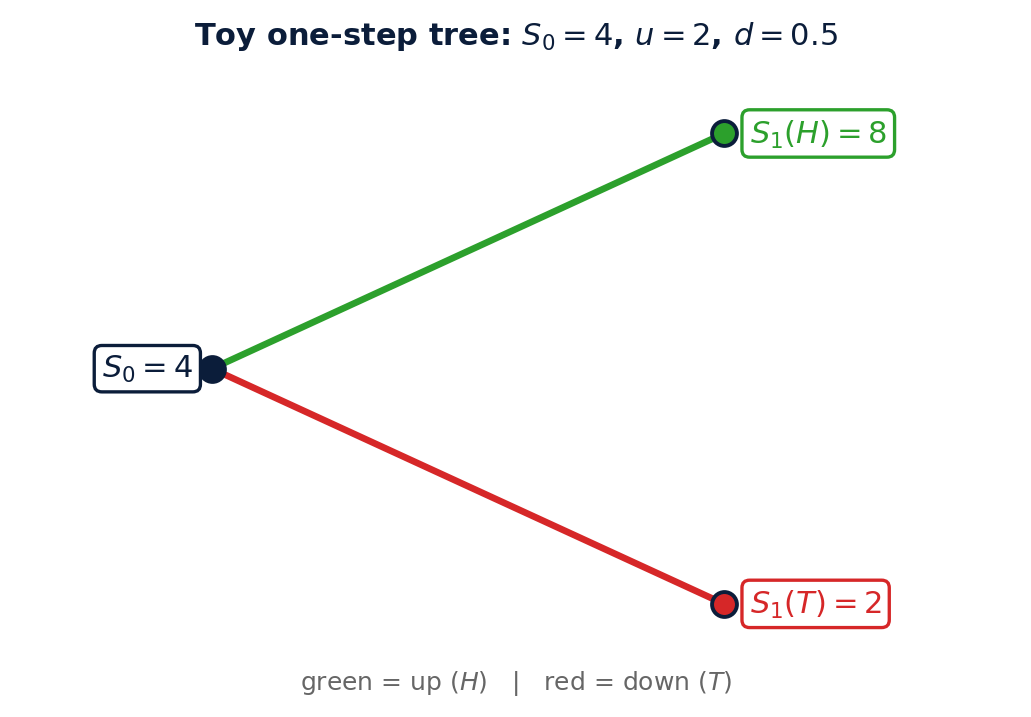
\includegraphics[keepaspectratio]{figures/ch01-tree-skeleton-st.png}}
\caption{One-step tree for the toy: root \(S_0=4\) branches to
\(S_1(H)=8\) and \(S_1(T)=2\). Edges colour-coded: green for the up
move, red for the down move. This skeleton --- root plus two leaves ---
is the only picture you need to keep in your head for the entire
chapter.}
\end{figure}

\begin{figure}
\centering
\pandocbounded{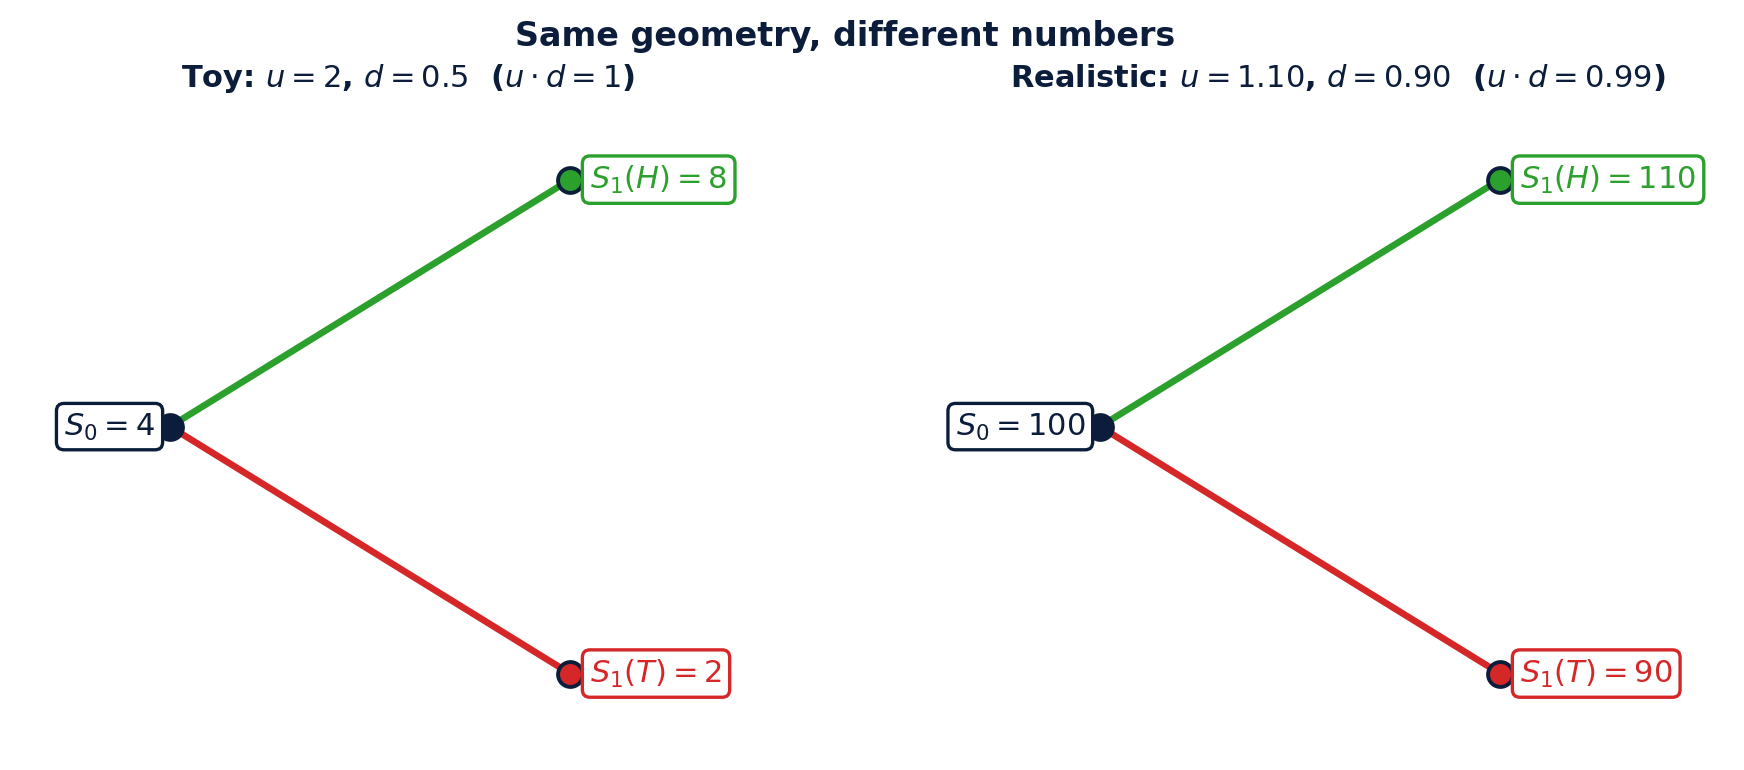
\includegraphics[keepaspectratio]{figures/ch01-tree-side-by-side.png}}
\caption{Toy (\(S_0=4,u=2,d=1/2\)) and the Realistic market
(\(S_0=100,u=1.10,d=0.90\)) side by side. The geometry is identical;
only the numbers differ. The Toy's \(u\) and \(d\) multiply to \(1\) (a
deliberate symmetry); the realistic market's \(u\cdot d = 0.99\) is
close to \(1\) but not exactly.}
\end{figure}

\textbf{Notation glossary} (we will refer to this throughout):

{\def\LTcaptype{none} % do not increment counter
\begin{table}[H]
\centering
\begin{tabular}{|l|l|}
\toprule
Symbol & Meaning \\
\midrule



\(S_0\) & stock price at \(t=0\) \\
\(S_1(\omega)\) & stock at \(t=1\), \(\omega\in\{H,T\}\) \\
\(u,d\) & up/down factors, \(0<d<u\) \\
\(r\) & one-period interest rate \\
\(1+r\) & bond gross return \\
\(1/(1+r)\) & discount factor \\
\(p,\,1-p\) & real-world prob. of \(H,T\) \\
\(\tilde p,\,1-\tilde p\) & risk-neutral prob. of \(H,T\) \\
\(V_1\) & payoff at \(t=1\) \\
\(V_u,V_d\) & \(V_1(H),V_1(T)\) \\
\(V_0\) & derivative price at \(t=0\) \\
\(\Delta,B\) & \(\Delta\) shares + \(B\) bond \\
\(X_1\) & portfolio value at \(t=1\) \\
\bottomrule
\end{tabular}
\end{table}
}

\emph{Notes.} \(r\) is one-period; in a single period continuous and
simple rates coincide. \(\tilde p\) is constructed from \(u,d,r\) in
§1.5.

\subsection{1.1.3 Portfolios and their
values}\label{portfolios-and-their-values}

A portfolio is a pair \((\Delta,B)\): hold \(\Delta\) shares of stock
(can be fractional, can be negative) and put \(B\) dollars in the bond
(can be negative, meaning \emph{borrow} \(|B|\)). Time-0 cost:

\[X_0 \;=\; \Delta\, S_0 + B.\]

Time-1 value, in either state:

\[X_1(\omega) \;=\; \Delta\, S_1(\omega) + B(1+r),\qquad \omega\in\{H,T\}.\]

So the random variable \(X_1\) is a pair of numbers:

\[X_1(H) = \Delta uS_0 + B(1+r), \qquad X_1(T) = \Delta dS_0 + B(1+r).\]

This is just linear algebra in two variables. The replication problem is
going to be: given a target pair \((V_u,V_d)\), find \((\Delta,B)\) that
makes \(X_1=V\) in both states. That is the 2×2 system from §0.11. We
solve it in §1.3.

\subsection{1.1.4 Derivative payoffs: a first
menagerie}\label{derivative-payoffs-a-first-menagerie}

Before we price anything, list the payoff pairs \((V_u,V_d)\) for the
standard derivatives. \emph{A derivative at \(t=1\) is a pair of numbers
--- nothing more.}

{\def\LTcaptype{none} % do not increment counter
\begin{table}[H]
\centering
\begin{tabular}{|l|l|l|}
\toprule
Derivative & \(V_u\) & \(V_d\) \\
\midrule



Call, \(K\) & \((uS_0-K)^+\) & \((dS_0-K)^+\) \\
Put, \(K\) & \((K-uS_0)^+\) & \((K-dS_0)^+\) \\
Forward, \(K\) & \(uS_0-K\) & \(dS_0-K\) \\
Cash digital & \(\mathbf 1_{uS_0>K}\) & \(\mathbf 1_{dS_0>K}\) \\
Asset digital & \(uS_0\,\mathbf 1_{uS_0>K}\) &
\(dS_0\,\mathbf 1_{dS_0>K}\) \\
Straddle, \(K\) & \(\lvert uS_0-K\rvert\) & \(\lvert dS_0-K\rvert\) \\
Power, exp 2 & \((uS_0)^2\) & \((dS_0)^2\) \\
Capped call, \((K,C)\) & \(((uS_0-K)^+)\wedge(C-K)\) &
\(((dS_0-K)^+)\wedge(C-K)\) \\
Custom & \(a\) & \(b\) \\
\bottomrule
\end{tabular}
\end{table}
}

\emph{Plain-English meanings.} \textbf{Call}: right to buy at \(K\).
\textbf{Put}: right to sell at \(K\). \textbf{Forward}: must buy at
\(K\) (no optionality). \textbf{Cash digital}: \$1 if ITM, else \$0.
\textbf{Asset digital}: receives the stock if ITM, else nothing.
\textbf{Straddle}: call + put = absolute distance from \(K\).
\textbf{Power, exp 2}: stock-squared payoff. \textbf{Capped call,
\((K,C)\)}: call but capped at \(C-K\). \textbf{Custom}: arbitrary pair
\((a,b)\).

\textbf{Example 1.1.1 (Toy, call \(K=5\)).} \(S_1\in\{8,2\}\), so
\(V_u=\max(8-5,0)=3\) and \(V_d=\max(2-5,0)=0\). The payoff is the pair
\((3,0)\). We will price this \emph{seven different ways} in the next
ten pages and get \(V_0=1.20\) every time.

\textbf{Example 1.1.2 (Toy, put \(K=5\)).} \(V_u=\max(5-8,0)=0\),
\(V_d=\max(5-2,0)=3\). Pair \((0,3)\).

\textbf{Example 1.1.3 (Toy, digital \(K=5\)).}
\(V_u=\mathbf{1}_{\{8>5\}}=1\), \(V_d=0\). Pair \((1,0)\).

\textbf{Example 1.1.4 (Toy, forward \(K=5\)).} \(V_u=8-5=3\),
\(V_d=2-5=-3\). Pair \((3,-3)\). Note the \emph{negative} number ---
forwards can lose money.

\textbf{Example 1.1.5 (RL, call \(K=100\)).} \(S_1\in\{110,90\}\).
\(V_u=10\), \(V_d=0\). Pair \((10,0)\).

\textbf{Example 1.1.6 (RL, put \(K=100\)).} \(V_u=0\), \(V_d=10\). Pair
\((0,10)\).

\textbf{Example 1.1.7 (RL, straddle \(K=100\)).} \(V_u=|110-100|=10\),
\(V_d=|90-100|=10\). Pair \((10,10)\). Constant payoff --- \emph{a
riskless instrument in disguise}; we will see in §1.5 that its price is
just \(10/(1+r)=10/1.02=9.804\).

\textbf{Example 1.1.8 (RL, power option, exp 2).} \(V_u=110^2=12100\),
\(V_d=90^2=8100\). Pair \((12100,8100)\). These big numbers are fine;
pricing is still a 2×2 system.

\subsection{1.1.5 Asset cheat-sheet}\label{asset-cheat-sheet}

{\def\LTcaptype{none} % do not increment counter
\begin{table}[H]
\centering
\begin{tabular}{|l|c|c|c|}
\toprule
Asset & Time-0 value & Time-1 value (\(H\)) & Time-1 value (\(T\)) \\
\midrule



Stock (ST) & \(4\) & \(8\) & \(2\) \\
Stock (RL) & \(100\) & \(110\) & \(90\) \\
Bond, \$1 invested (ST) & \(1\) & \(1.25\) & \(1.25\) \\
Bond, \$1 invested (RL) & \(1\) & \(1.02\) & \(1.02\) \\
ST call, \(K=5\) & \(V_0=?\) & \(3\) & \(0\) \\
RL call, \(K=100\) & \(V_0=?\) & \(10\) & \(0\) \\
\bottomrule
\end{tabular}
\end{table}
}

The two unknown numbers in the last column are the answers we will
compute, six different times each.

\subsection{1.1.6 Exercises}\label{exercises-11}

\begin{enumerate}
\def\labelenumi{\arabic{enumi}.}
\tightlist
\item
  In RL, what is the put payoff for \(K=95\)? \textbf{Answer:}
  \(V_u=0\), \(V_d=\max(95-90,0)=5\). Pair \((0,5)\).
\item
  In ST, what is the digital with \(K=10\)? \textbf{Answer:}
  \(\mathbf{1}_{\{8>10\}}=0\), \(\mathbf{1}_{\{2>10\}}=0\). Pair
  \((0,0)\). A worthless option.
\item
  In ST, what is the straddle with \(K=4\)? \textbf{Answer:}
  \(|8-4|=4\), \(|2-4|=2\). Pair \((4,2)\).
\end{enumerate}

\begin{center}\rule{0.5\linewidth}{0.5pt}\end{center}

\section{\texorpdfstring{§1.2 Arbitrage and the no-arbitrage condition
\(d < 1+r < u\)}{§1.2 Arbitrage and the no-arbitrage condition d \textless{} 1+r \textless{} u}}\label{arbitrage-and-the-no-arbitrage-condition-d-1r-u}

\textbf{Punchline.} The single-period market admits \emph{no arbitrage}
if and only if \(d < 1+r < u\). Break either inequality and a riskless
profit can be locked in at \(t=0\).

\textbf{Intuition.} \(1+r\) is the gross return of the bond ---
\emph{the} benchmark. The stock returns either \(u\) or \(d\) in gross
terms. If the bond beats the stock in \emph{both} states
(\(1+r \ge u > d\)), you should borrow stock (short it), invest in the
bond, and you win in both states. If the bond loses to the stock in
\emph{both} states (\(d \ge 1+r\)), you should borrow at the bond rate,
buy the stock, and you win in both states. The only way to make the
market interesting --- i.e.~to make the stock genuinely a \emph{risky}
alternative --- is to sandwich the bond's return strictly between \(d\)
and \(u\).

\subsection{1.2.1 What is arbitrage?}\label{what-is-arbitrage}

A \emph{portfolio strategy} in our one-period market is a choice of
\((\Delta,B)\) at \(t=0\). We say it is an \textbf{arbitrage} if all
three hold:

\begin{enumerate}
\def\labelenumi{\arabic{enumi}.}
\tightlist
\item
  \(X_0 = \Delta S_0 + B \le 0\) (you start with non-positive cash ---
  possibly negative, meaning the trade pays you up front).
\item
  \(X_1(\omega) \ge 0\) in both states \(\omega\in\{H,T\}\) (you never
  lose at \(t=1\)).
\item
  \(X_1(\omega) > 0\) in at least one state (you sometimes win).
\end{enumerate}

The strongest form (which we will mostly use) is \(X_0 = 0\) and
\(X_1 \ge 0\) with strict inequality somewhere. \emph{No money in, never
lose, sometimes win.} That is a money-printing machine.

\subsection{1.2.2 The theorem}\label{the-theorem}

\textbf{Theorem (no-arbitrage).} The one-period binomial market
\((S_0,u,d,r)\) admits no arbitrage if and only if \(d<1+r<u\).

\textbf{Proof, both directions.}

\emph{Suppose \(d<1+r<u\) holds (the ``good'' case).} Take any portfolio
\((\Delta,B)\) with \(X_0=0\), i.e.~\(B=-\Delta S_0\). Then

\[X_1(H) = \Delta uS_0 + B(1+r) = \Delta S_0(u - (1+r)),\]
\[X_1(T) = \Delta dS_0 + B(1+r) = \Delta S_0(d - (1+r)).\]

In the good case \(u-(1+r)>0\) and \(d-(1+r)<0\). So if \(\Delta>0\),
then \(X_1(H)>0\) but \(X_1(T)<0\) --- not an arbitrage. If
\(\Delta<0\), then \(X_1(H)<0\) and \(X_1(T)>0\) --- not an arbitrage
either. If \(\Delta=0\), then \(B=0\) and the portfolio is identically
zero --- not an arbitrage. So \emph{no} zero-cost portfolio can be a
``never lose'' portfolio. ✓

\emph{Suppose \(1+r\ge u\) (the ``bond dominates'' case).} The portfolio
\(\Delta=-1, B=S_0\) (short one share, lend \(S_0\)) has \(X_0=0\).
Time-1 value:

\[X_1(H) = -uS_0 + S_0(1+r) = S_0(1+r-u) \ge 0,\]
\[X_1(T) = -dS_0 + S_0(1+r) = S_0(1+r-d) > 0\]

(the second is strict because \(1+r\ge u>d\)). That is an arbitrage. ✓

\emph{Suppose \(d\ge 1+r\) (the ``stock dominates'' case).} The
portfolio \(\Delta=+1, B=-S_0\) (long one share, borrow \(S_0\)) has
\(X_0=0\).

\[X_1(H) = uS_0 - S_0(1+r) = S_0(u-(1+r)) > 0,\]
\[X_1(T) = dS_0 - S_0(1+r) = S_0(d-(1+r)) \ge 0.\]

Again an arbitrage. ✓

So both halves of the iff are proved.

\subsection{1.2.3 Picturing the
condition}\label{picturing-the-condition}

The condition \(d<1+r<u\) is one inequality on three numbers. On the
real line: place \(1+r\) in the middle, with \(d\) to its left and \(u\)
to its right.

\begin{figure}
\centering
\pandocbounded{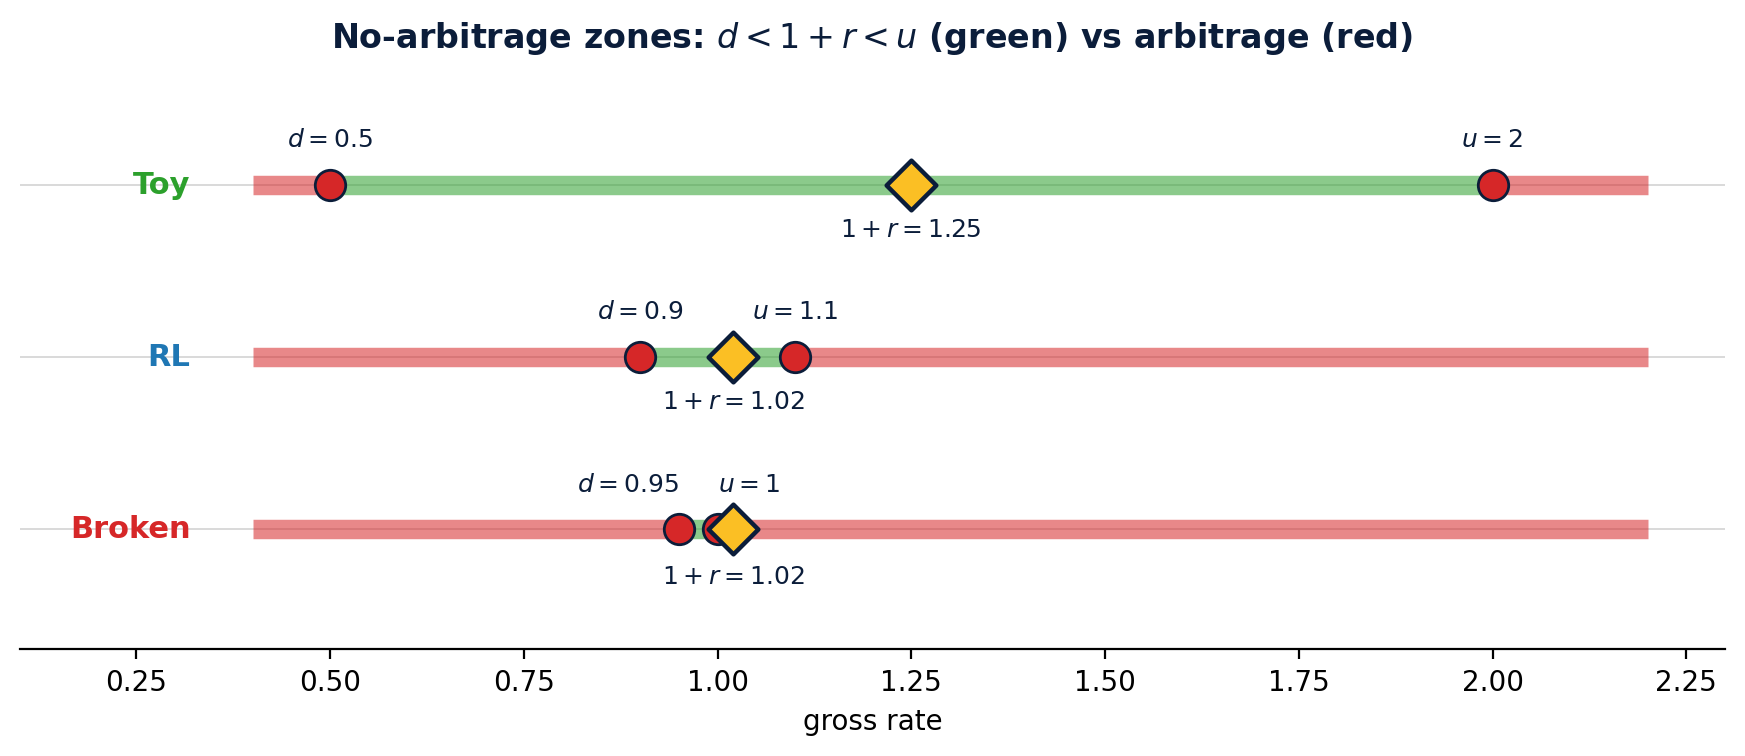
\includegraphics[keepaspectratio]{figures/ch01-noarb-zones.png}}
\caption{No-arbitrage zones on the number line. The green segment
\((d,u)\) is where \(1+r\) must live. Red segments \((-\infty,d]\) and
\([u,\infty)\) are arbitrage zones: stock dominates bond, or bond
dominates stock. Three markets plotted: Toy (\(d=0.5, 1+r=1.25, u=2\))
is well-centred; RL (\(0.90, 1.02, 1.10\)) is also centred; a broken
example (\(0.95, 1.02, 1.00\)) shows \(1+r > u\), an arbitrage.}
\end{figure}

\subsection{1.2.4 Worked verifications}\label{worked-verifications}

\textbf{Example 1.2.1 (Toy, no-arb check).} \(d=0.5\), \(1+r=1.25\),
\(u=2\). Is \(0.5<1.25<2\)? Yes. No arbitrage. ✓

\textbf{Example 1.2.2 (RL, no-arb check).} \(d=0.90\), \(1+r=1.02\),
\(u=1.10\). Is \(0.90<1.02<1.10\)? Yes. ✓

\textbf{Example 1.2.3 (broken: bond dominates).} Let \(u=1.01\),
\(d=0.97\), \(r=0.02\) so \(1+r=1.02>u=1.01\). The arbitrage: short one
share, lend \(S_0\). Cash at \(t=0\): \(0\). Cash at \(t=1\):

\begin{itemize}
\tightlist
\item
  \(H\): \(-1.01 S_0 + 1.02 S_0 = +0.01 S_0\).
\item
  \(T\): \(-0.97 S_0 + 1.02 S_0 = +0.05 S_0\).
\end{itemize}

Both strictly positive. \emph{Profit guaranteed}. With \(S_0=100\), you
make at least \(\$1\) per share and as much as \(\$5\), for zero
up-front cost.

\textbf{Example 1.2.4 (broken: stock dominates).} Let \(u=1.10\),
\(d=1.03\), \(r=0.02\) so \(d=1.03>1.02=1+r\). The arbitrage: long one
share, borrow \(S_0\). Cash at \(t=0\): \(0\). Cash at \(t=1\):

\begin{itemize}
\tightlist
\item
  \(H\): \(1.10 S_0 - 1.02 S_0 = +0.08 S_0\).
\item
  \(T\): \(1.03 S_0 - 1.02 S_0 = +0.01 S_0\).
\end{itemize}

Both strictly positive.

\textbf{Example 1.2.5 (marginal: \(1+r = u\)).}
\(u=1.05, d=0.97, r=0.05\). Now \(1+r=u\). The ``bond dominates''
arbitrage still works \emph{weakly} --- in \(H\) you make exactly zero,
in \(T\) you make \(S_0(1.05-0.97)=0.08 S_0>0\). It is still an
arbitrage (the third condition requires strict positivity only in
\emph{one} state). So the strict inequality matters: \(d<1+r<u\) must
hold strictly.

\textbf{Example 1.2.6 (marginal: \(d=1+r\)).} Symmetric to the above;
\(\Delta=+1, B=-S_0\) gives an arbitrage with strict profit only in
\(H\).

\textbf{Example 1.2.7 (negative rates).} Let \(r=-0.01\), \(u=1.05\),
\(d=0.97\), so \(1+r=0.99\). Is \(0.97<0.99<1.05\)? Yes. No arbitrage.
Negative rates are fine as long as \(d<1+r\) still holds. In the
post-2014 European bond market this case was the norm.

\textbf{Example 1.2.8 (the bond is just an asset).} If instead of a bond
you had a second risky asset that paid \(1+r\) in both states, the
analysis is identical. The ``bond'' is a placeholder for ``any asset
with a deterministic return.'' Sometimes called the \emph{numéraire}.

\subsection{1.2.5 Arbitrage cashflow
diagram}\label{arbitrage-cashflow-diagram}

\begin{figure}
\centering
\pandocbounded{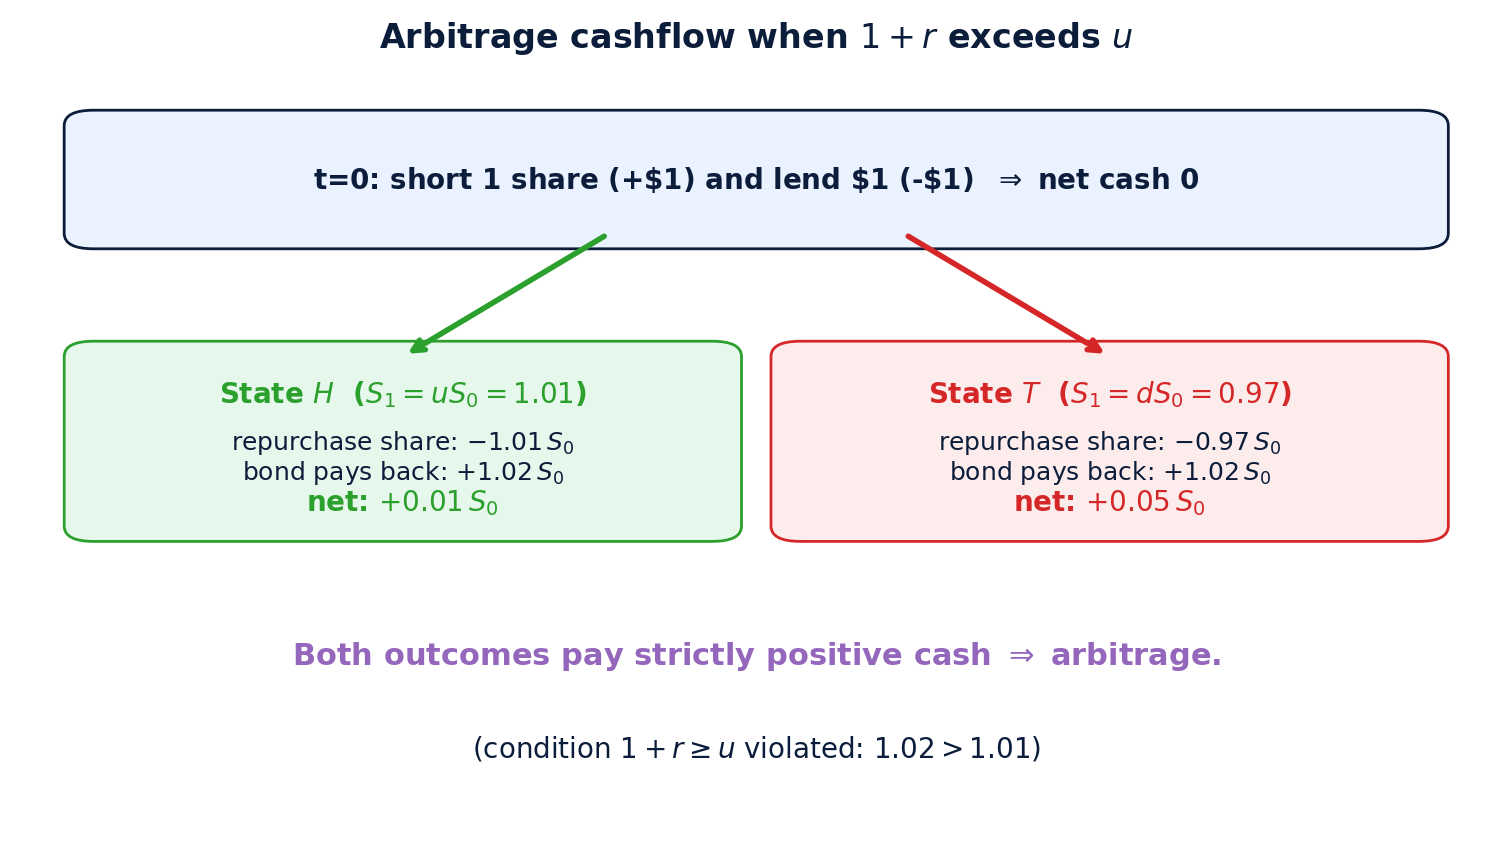
\includegraphics[keepaspectratio]{figures/ch01-arb-cashflow.png}}
\caption{Cashflow diagram for the broken-up arbitrage in Example 1.2.3
(\(u=1.01, d=0.97, 1+r=1.02\)). Top bar: \(t=0\) position --- short one
share (+\(S_0\) cash) and lend \(S_0\) (-\(S_0\) cash) --- net zero.
Bottom-left bar: in state \(H\), repurchase share at \(1.01 S_0\)
(-\(1.01 S_0\)), bond pays back \(1.02 S_0\) (+\(1.02 S_0\)) --- net
\(+0.01 S_0\). Bottom-right bar: in state \(T\), repurchase share at
\(0.97 S_0\), bond pays \(1.02 S_0\) --- net \(+0.05 S_0\). Both
positive --- riskless profit.}
\end{figure}

\subsection{1.2.6 Four-quadrant table}\label{four-quadrant-table}

{\def\LTcaptype{none} % do not increment counter
\begin{table}[H]
\centering
\begin{tabular}{|l|c|c|}
\toprule
Case & Condition & Arb portfolio \((\Delta,B)\) \\
\midrule



Good market & \(d<1+r<u\) & none \\
Bond dominates & \(1+r\ge u\) & \((-1,\,+S_0)\) \\
Stock dominates & \(d \ge 1+r\) & \((+1,\,-S_0)\) \\
Both fail & impossible since \(d<u\) & --- \\
\bottomrule
\end{tabular}
\end{table}
}

\emph{Profit signs.} When \textbf{bond dominates}, the portfolio
\((-1,+S_0)\) pays \(\ge 0\) in state \(H\) and \(>0\) in state \(T\)
(strictly positive at least once: free money). When \textbf{stock
dominates}, the portfolio \((+1,-S_0)\) pays \(>0\) in \(H\) and
\(\ge 0\) in \(T\).

\emph{Blank: no arbitrage portfolio exists or case is vacuous.}

\subsection{1.2.7 Test parameter triples}\label{test-parameter-triples}

\textbf{Table 1.2.} Eight \((u,d,r)\) triples and whether the market is
arbitrage-free.

{\def\LTcaptype{none} % do not increment counter
\begin{table}[H]
\centering
\begin{tabular}{|r|r|r|r|c|l|}
\toprule
\(u\) & \(d\) & \(r\) & \(1+r\) & \(d<1+r<u\)? & Verdict \\
\midrule



\(2.00\) & \(0.50\) & \(\phantom{-}0.25\) & \(1.25\) & Yes & OK \\
\(1.10\) & \(0.90\) & \(\phantom{-}0.02\) & \(1.02\) & Yes & OK \\
\(1.10\) & \(0.90\) & \(\phantom{-}0.15\) & \(1.15\) & No & Short \\
\(1.05\) & \(0.95\) & \(-0.01\) & \(0.99\) & Yes & OK \\
\(1.20\) & \(1.05\) & \(\phantom{-}0.10\) & \(1.10\) & Yes & OK \\
\(1.50\) & \(0.80\) & \(\phantom{-}0.05\) & \(1.05\) & Yes & OK \\
\(1.01\) & \(0.99\) & \(\phantom{-}0.02\) & \(1.02\) & No & Short \\
\(1.05\) & \(1.03\) & \(\phantom{-}0.02\) & \(1.02\) & No & Long \\
\(1.00\) & \(1.00\) & \(\phantom{-}0.00\) & \(1.00\) & No & Degen \\
\bottomrule
\end{tabular}
\end{table}
}

\emph{Legend.} OK = \(d<1+r<u\), no arbitrage. Short = bond dominates
(\(1+r\ge u\)); short the stock, long the bond. Long = stock dominates
(\(d\ge 1+r\)); long the stock, short the bond. Degen = \(u=d\), no
randomness.

The last row is a market with no randomness; pricing is trivial
(everything = bond) and the no-arbitrage \emph{strict} inequality fails
because there's nothing to sandwich.

\subsection{1.2.8 Exercises}\label{exercises-12}

\begin{enumerate}
\def\labelenumi{\arabic{enumi}.}
\tightlist
\item
  Show that \(u=1.30, d=0.85, r=0.10\) is arb-free. \textbf{Answer:}
  \(0.85<1.10<1.30\). ✓
\item
  For \(u=1.05, d=1.03, r=0.02\), find the arb. \textbf{Answer:}
  \(1+r=1.02<d=1.03\), so the stock dominates. Long one share, borrow
  \(S_0\): \(X_0=0\). In \(H\),
  \(X_1 = (1.05-1.02)S_0 = 0.03\,S_0 > 0\); in \(T\),
  \(X_1 = (1.03-1.02)S_0 = 0.01\,S_0 > 0\). Both strictly positive ---
  guaranteed profit.
\item
  What is the \emph{symmetric} boundary case
  (\(1+r = \tfrac{1}{2}(u+d)\))? \textbf{Answer:} Just a centred market;
  no special significance for arbitrage as long as the strict
  inequalities hold.
\end{enumerate}

\begin{center}\rule{0.5\linewidth}{0.5pt}\end{center}

\section{§1.3 Replicating a derivative
payoff}\label{replicating-a-derivative-payoff}

\textbf{Punchline.} Given any pair of numbers \((V_u, V_d)\), there is a
unique portfolio \((\Delta, B)\) whose time-1 value is \(V_u\) in state
\(H\) and \(V_d\) in state \(T\). The formulas are

\[\boxed{\Delta \;=\; \frac{V_u - V_d}{(u-d)S_0}, \qquad B \;=\; \frac{uV_d - dV_u}{(u-d)(1+r)}.}\]

The cost of building this portfolio at \(t=0\) is \(\Delta S_0 + B\) ---
that is the \emph{replication price} of the derivative.

\textbf{Intuition.} A derivative payoff is two numbers. The portfolio
has two knobs (\(\Delta\) and \(B\)). The map from knobs to payoff is
\emph{linear} (each knob produces a linear contribution to each state).
So it is a 2×2 linear system in two unknowns, and §0.11 says that has a
unique solution whenever the system isn't degenerate. The only way the
system is degenerate is \(u=d\) --- which we ruled out. Replication is
therefore \emph{automatic}: any payoff can be built from stock and bond,
full stop.

\subsection{1.3.1 Deriving the formulas}\label{deriving-the-formulas}

We want \(X_1(H) = V_u\) and \(X_1(T) = V_d\), i.e.,

\[\Delta\, uS_0 + B(1+r) = V_u,\] \[\Delta\, dS_0 + B(1+r) = V_d.\]

Subtract the second from the first:

\[\Delta(u - d)S_0 = V_u - V_d \quad\Longrightarrow\quad \Delta = \frac{V_u - V_d}{(u-d)S_0}.\]

This is the \emph{delta} of the derivative --- the number of shares you
must hold. The formula says \textbf{delta is the rise-over-run of the
payoff across the two states}, normalised by \(S_0\).

Now solve for \(B\). Use the second equation:

\[B(1+r) = V_d - \Delta\, dS_0 = V_d - \frac{d(V_u-V_d)}{u-d} = \frac{(u-d)V_d - d(V_u-V_d)}{u-d} = \frac{uV_d - dV_u}{u-d}.\]

Divide by \(1+r\) to finish.

The replication price is

\[V_0 \;=\; \Delta\, S_0 + B \;=\; \frac{V_u-V_d}{u-d} + \frac{uV_d - dV_u}{(u-d)(1+r)}.\]

We will simplify this expression in §1.5 and recognise the result as a
risk-neutral expectation. For now we just compute it on examples.

\subsection{1.3.2 Worked examples --- Toy
menagerie}\label{worked-examples-toy-menagerie}

In all of these, \(S_0=4\), \(u=2\), \(d=0.5\), \(r=0.25\), so
\(u-d=1.5\), \((u-d)S_0=6\), \(1+r=1.25\), \((u-d)(1+r)=1.875\).

\textbf{Example 1.3.1 (ST call, \(K=5\)).} \(V_u=3, V_d=0\).
\[\Delta = \frac{3-0}{6} = 0.5, \qquad B = \frac{2\cdot 0 - 0.5\cdot 3}{1.875} = \frac{-1.5}{1.875} = -0.8.\]
Cost: \(V_0 = 0.5\cdot 4 + (-0.8) = 2.0 - 0.8 = \boxed{1.20}\). Hold
half a share, borrow \(\$0.80\).

\emph{Check.} Time-1 in \(H\):
\(0.5\cdot 8 + (-0.8)\cdot 1.25 = 4 - 1 = 3 = V_u\). ✓ Time-1 in \(T\):
\(0.5\cdot 2 - 1 = 0 = V_d\). ✓

\textbf{Example 1.3.2 (ST put, \(K=5\)).} \(V_u=0, V_d=3\).
\[\Delta = \frac{0-3}{6} = -0.5, \qquad B = \frac{2\cdot 3 - 0.5\cdot 0}{1.875} = \frac{6}{1.875} = 3.2.\]
Cost: \(V_0 = -0.5\cdot 4 + 3.2 = -2 + 3.2 = \boxed{1.20}\). Same price
as the call! (Coincidence in this symmetric toy: see Example 1.9.1 on
parity.)

\emph{Check.} Time-1 in \(H\):
\(-0.5\cdot 8 + 3.2\cdot 1.25 = -4 + 4 = 0\). ✓ Time-1 in \(T\):
\(-0.5\cdot 2 + 4 = 3\). ✓

\textbf{Example 1.3.3 (ST digital, \(K=5\)).} \(V_u=1, V_d=0\).
\[\Delta = \frac{1}{6}, \qquad B = \frac{-0.5}{1.875} = -\frac{4}{15}.\]
Cost:
\(\frac{1}{6}\cdot 4 - \frac{4}{15} = \frac{2}{3} - \frac{4}{15} = \frac{10-4}{15} = \frac{6}{15} = 0.40\).

\textbf{Example 1.3.4 (ST forward, \(K=5\)).} \(V_u=3, V_d=-3\).
\[\Delta = \frac{3-(-3)}{6} = 1, \qquad B = \frac{2(-3) - 0.5(3)}{1.875} = \frac{-7.5}{1.875} = -4.\]
Cost: \(1\cdot 4 - 4 = 0\). A forward struck at \(K=5\) costs zero today
--- meaning the ``fair forward price'' \(F\) is the one that makes the
forward cost zero. Solving \(S_0 - F/(1+r) = 0\) gives
\(F = (1+r)S_0 = 5\). ✓

\textbf{Example 1.3.5 (ST asset-or-nothing, \(K=5\)).} \(V_u=8, V_d=0\).
\[\Delta = \frac{8}{6} = \tfrac{4}{3}, \qquad B = \frac{-4}{1.875} = -\tfrac{32}{15}.\]
Cost:
\(\tfrac{4}{3}\cdot 4 - \tfrac{32}{15} = \tfrac{16}{3} - \tfrac{32}{15} = \tfrac{80-32}{15} = \tfrac{48}{15} = 3.20\).

\textbf{Example 1.3.6 (ST straddle, \(K=4\)).} \(V_u=4, V_d=2\).
\[\Delta = \frac{2}{6} = \tfrac{1}{3}, \qquad B = \frac{2\cdot 2 - 0.5\cdot 4}{1.875} = \frac{2}{1.875} = \tfrac{16}{15}.\]
Cost:
\(\tfrac{1}{3}\cdot 4 + \tfrac{16}{15} = \tfrac{4}{3} + \tfrac{16}{15} = \tfrac{20+16}{15} = \tfrac{36}{15} = 2.40\).

\textbf{Example 1.3.7 (ST custom payoff \((25,-5)\)).} Suppose a
structured product pays \(\$25\) in \(H\) and \emph{charges} \(\$5\) in
\(T\).
\[\Delta = \frac{25-(-5)}{6} = 5, \qquad B = \frac{2(-5) - 0.5(25)}{1.875} = \frac{-22.5}{1.875} = -12.\]
Cost: \(5\cdot 4 - 12 = 8.\) \emph{Verification:} time-1 in \(H\):
\(5\cdot 8 -12\cdot 1.25 = 40-15 = 25\). ✓ In \(T\):
\(5\cdot 2 - 12\cdot 1.25 = 10-15 = -5\). ✓

\textbf{Example 1.3.8 (ST power option, exp 2).} \(V_u=8^2=64\),
\(V_d=2^2=4\).
\[\Delta = \frac{60}{6} = 10, \qquad B = \frac{2\cdot 4 - 0.5\cdot 64}{1.875} = \frac{-24}{1.875} = -12.8.\]
Cost: \(10\cdot 4 - 12.8 = 27.20\).

\textbf{Example 1.3.9 (ST capped call, \(K=4,C=6\)).} Call payoffs
\((4,0)\), but capped at \(C-K=2\): \(V_u=\min(4,2)=2\), \(V_d=0\).
\[\Delta = \frac{2}{6} = \tfrac{1}{3}, \qquad B = \frac{-1}{1.875} = -\tfrac{8}{15}.\]
Cost:
\(\tfrac{1}{3}\cdot 4 - \tfrac{8}{15} = \tfrac{20-8}{15} = \tfrac{12}{15} = 0.80\).

\subsection{1.3.3 Worked examples --- Realistic
menagerie}\label{worked-examples-realistic-menagerie}

Here \(S_0=100\), \(u=1.10\), \(d=0.90\), \(r=0.02\), so \(u-d=0.20\),
\((u-d)S_0 = 20\), \(1+r=1.02\), \((u-d)(1+r)=0.204\).

\textbf{Example 1.3.10 (RL call, \(K=100\)).} \(V_u=10, V_d=0\).
\[\Delta = \frac{10}{20} = 0.5, \qquad B = \frac{1.10(0) - 0.90(10)}{0.204} = \frac{-9}{0.204} = -44.117647\ldots\]
Cost: \(0.5(100) - 44.1176 = 50 - 44.1176 = \boxed{5.8824}\).

\textbf{Example 1.3.11 (RL put, \(K=100\)).} \(V_u=0, V_d=10\).
\[\Delta = \frac{-10}{20} = -0.5, \qquad B = \frac{1.10(10) - 0}{0.204} = \frac{11}{0.204} = 53.9216.\]
Cost: \(-50 + 53.9216 = \boxed{3.9216}\).

\textbf{Example 1.3.12 (RL digital, \(K=100\)).} \(V_u=1, V_d=0\).
\[\Delta = \frac{1}{20} = 0.05, \qquad B = \frac{0 - 0.90}{0.204} = -4.4118.\]
Cost: \(0.05(100) - 4.4118 = 5 - 4.4118 = 0.5882\).

\textbf{Example 1.3.13 (RL straddle, \(K=100\)).} \(V_u=10, V_d=10\).
\[\Delta = 0, \qquad B = \frac{1.10(10) - 0.90(10)}{0.204} = \frac{2}{0.204} = 9.8039.\]
Cost: \(0 + 9.8039 = 9.8039\). \emph{Equal to \(10/(1+r)\)}, the
discounted certain payoff. The portfolio is entirely in the bond,
because the payoff is deterministic --- no hedge needed.

\textbf{Example 1.3.14 (RL forward, \(K=100\)).} \(V_u=10, V_d=-10\).
\[\Delta = \frac{20}{20} = 1, \qquad B = \frac{1.10(-10) - 0.90(10)}{0.204} = \frac{-20}{0.204} = -98.0392.\]
Cost: \(100 - 98.0392 = 1.9608\). The forward struck at \(100\) costs
\(\$1.96\) today. The \emph{fair forward price} (the strike that costs
zero) is \((1+r)S_0 = 102\).

\textbf{Example 1.3.15 (RL forward struck at \(102\)).}
\(V_u=8, V_d=-12\).
\[\Delta = 1, \qquad B = \frac{1.10(-12) - 0.90(8)}{0.204} = \frac{-20.4}{0.204} = -100.\]
Cost: \(100 - 100 = 0\). ✓

\textbf{Example 1.3.16 (RL risk-reversal).} Long call \(K=110\), short
put \(K=90\). Payoffs: call\((110)\) gives \(V_u=0, V_d=0\); put\((90)\)
gives \(V_u=0, V_d=0\). The risk-reversal here is identically zero ---
useless example with these specific strikes. Try call\((K=100)\) minus
put\((K=100)\): payoffs \((10,0)-(0,10) = (10,-10)\) --- same as the
forward at \(K=100\). So this risk-reversal \emph{is} a forward; cost
\(\$1.96\) as in 1.3.14. The put-call parity in §1.9 will make this
exact.

\textbf{Example 1.3.17 (RL power option, exp 2).}
\(V_u=110^2=12100, V_d=90^2=8100\). \[
\begin{aligned}
\Delta &= \frac{4000}{20} = 200, \\
B &= \frac{1.10(8100) - 0.90(12100)}{0.204}
  = \frac{8910 - 10890}{0.204}
  = \frac{-1980}{0.204}
  = -9705.88.
\end{aligned}
\] Cost: \(200(100) - 9705.88 = 20000 - 9705.88 = 10294.12\).

\textbf{Example 1.3.18 (RL capped call, \(K=100, C=105\)).} Call payoffs
are \((10,0)\) capped at \(5\): \(V_u=5, V_d=0\).
\[\Delta = 0.25, \qquad B = \frac{0 - 0.90(5)}{0.204} = -22.0588.\]
Cost: \(25 - 22.0588 = 2.9412\). \emph{Half} the price of the uncapped
RL call (\(5.8824\)).

\subsection{1.3.4 Replication-wheel and 3-D delta
plane}\label{replication-wheel-and-3-d-delta-plane}

\begin{figure}
\centering
\pandocbounded{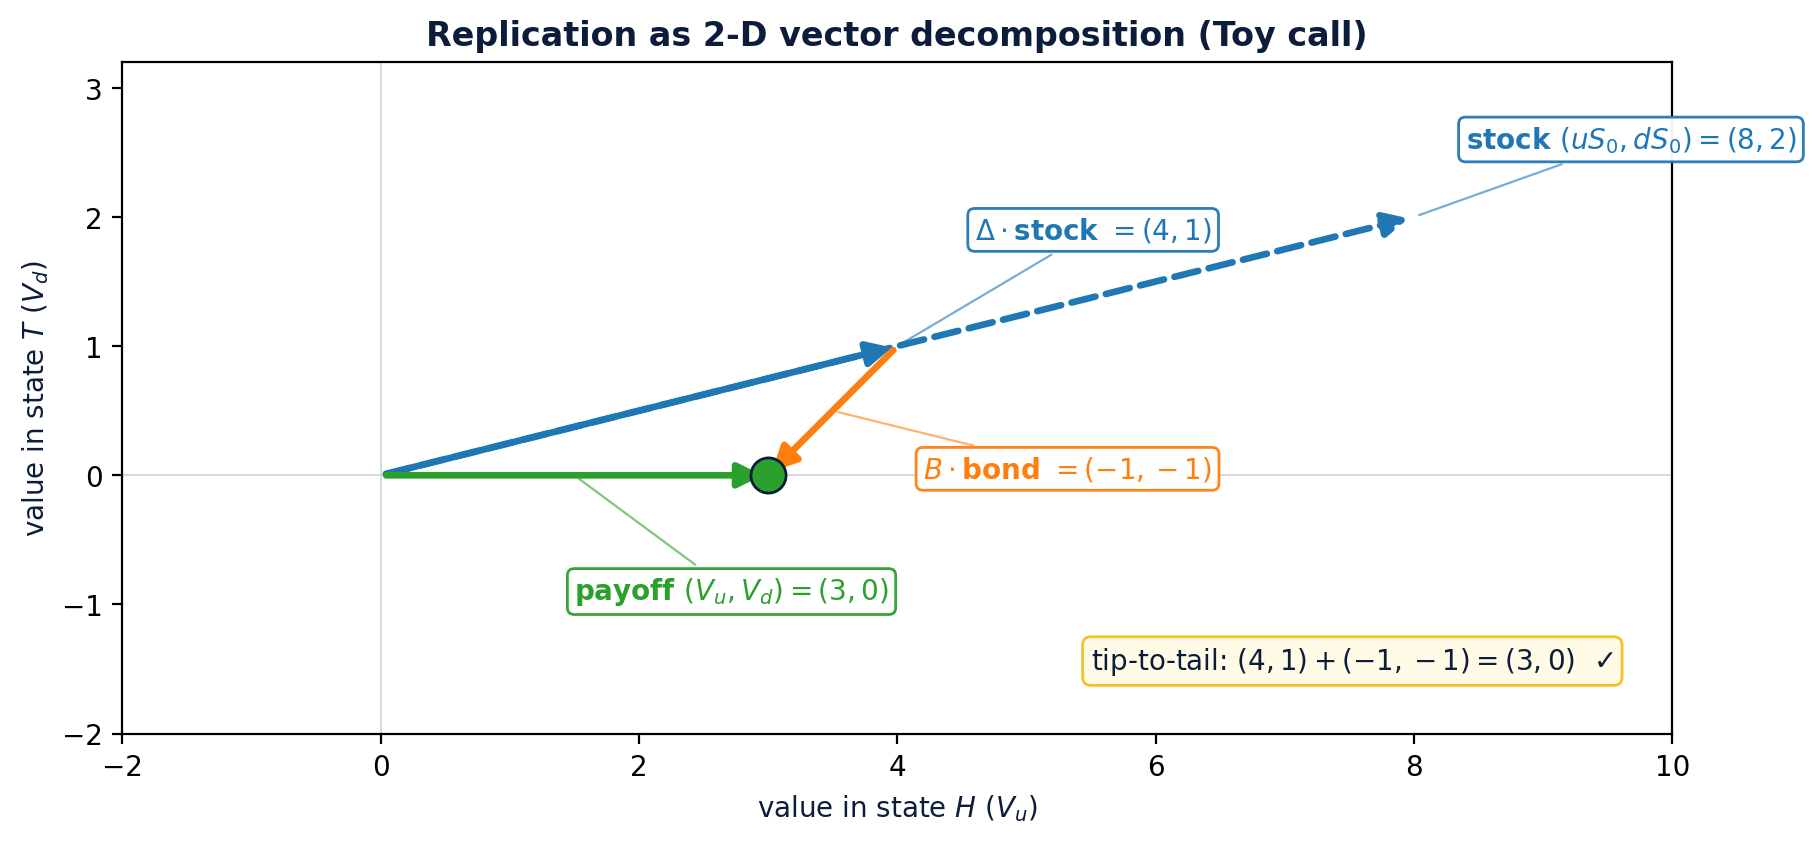
\includegraphics[keepaspectratio]{figures/ch01-replication-wheel.png}}
\caption{Replication as 2-D vector decomposition. The payoff
\((V_u,V_d)=(3,0)\) (ST call) is the sum of \(\Delta=0.5\) copies of the
stock vector \((uS_0,dS_0)=(8,2)\) --- namely \((4,1)\) --- and \(-0.8\)
copies of the bond vector \((1+r,1+r)=(1.25,1.25)\) --- namely
\((-1,-1)\). Tip-to-tail: \((4,1)+(-1,-1)=(3,0)\). ✓ The stock vector
and bond vector span the entire 2-D plane; any payoff can be reached.}
\end{figure}

\begin{figure}
\centering
\pandocbounded{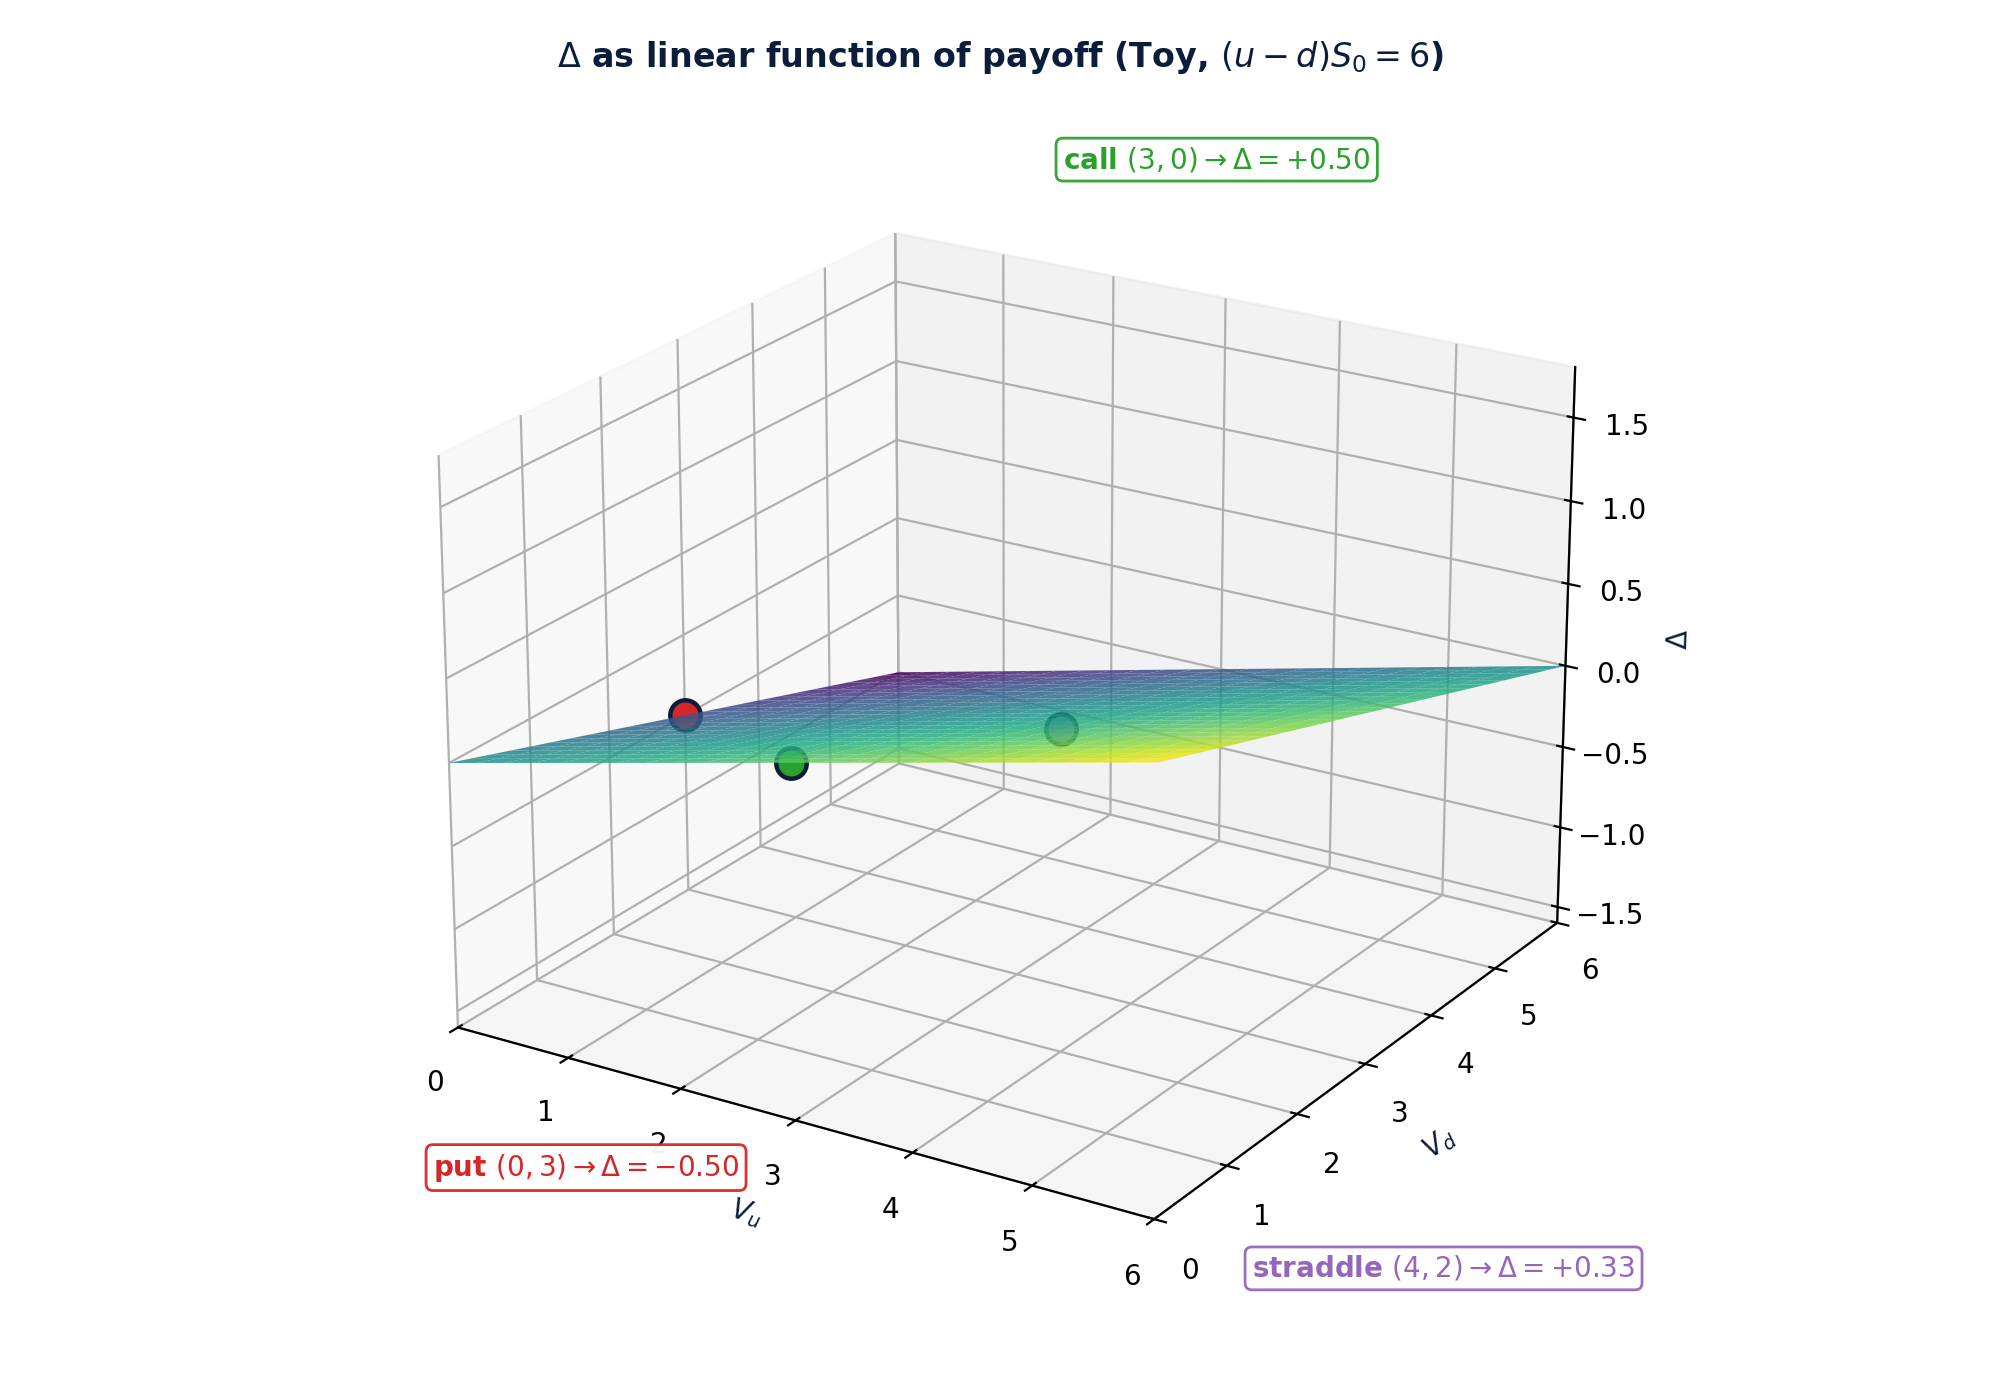
\includegraphics[keepaspectratio]{figures/ch01-delta-plane-3d.png}}
\caption{3-D plane showing \(\Delta=(V_u-V_d)/((u-d)S_0)\) as a linear
function of the payoff pair \((V_u,V_d)\). For the ST world the plane
has slope \(+1/6\) in the \(V_u\) direction and \(-1/6\) in the \(V_d\)
direction. Three derivatives plotted on the surface: call
\((3,0)\mapsto 0.5\), put \((0,3)\mapsto -0.5\), straddle
\((4,2)\mapsto 0.33\).}
\end{figure}

\begin{figure}
\centering
\pandocbounded{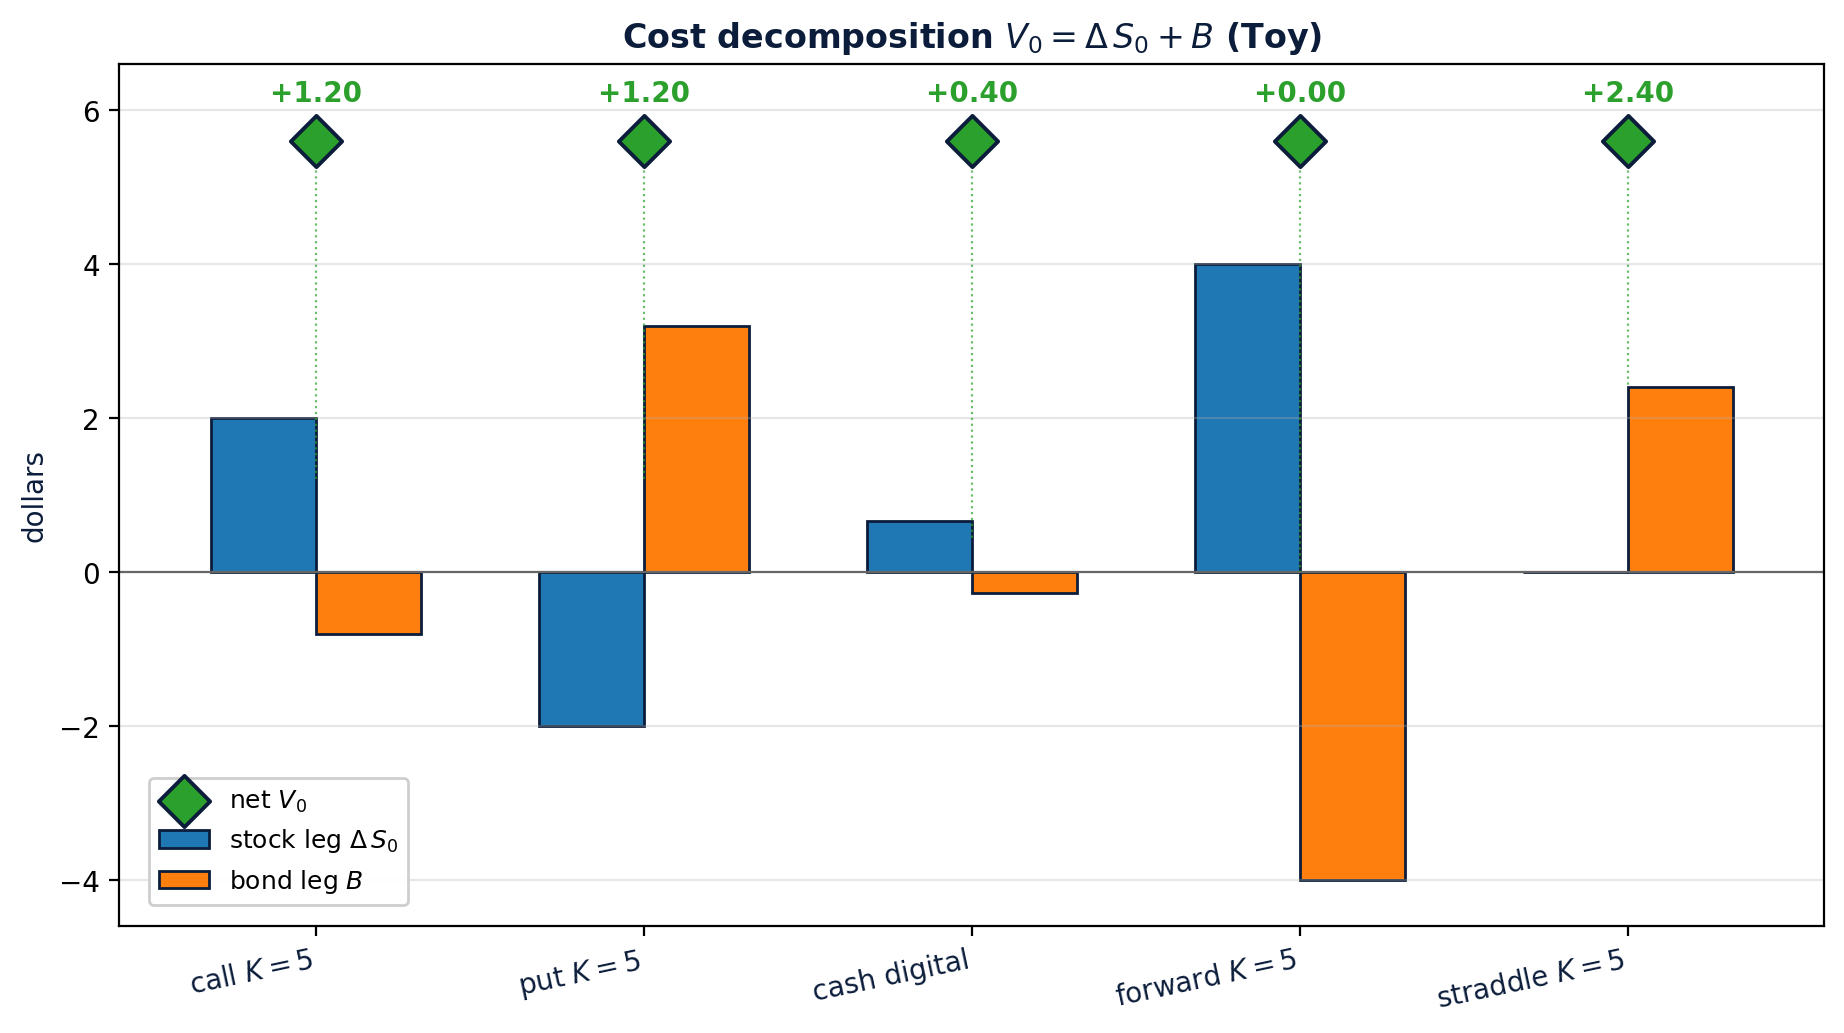
\includegraphics[keepaspectratio]{figures/ch01-cost-decomposition.png}}
\caption{Cost decomposition \(V_0 = \Delta S_0 + B\) for six ST
derivatives. Each bar is a derivative's price split into the \emph{stock
leg} (\(\Delta S_0\), blue, can be positive or negative) and the
\emph{bond leg} (\(B\), orange). For the call: stock leg \(+2.0\), bond
leg \(-0.8\) (you're financing the stock by borrowing); net \(1.20\).
For the put the legs flip sign.}
\end{figure}

\subsection{1.3.5 Replication cookbook}\label{replication-cookbook}

\textbf{Table 1.3.} Toy (\(S_0=4,u=2,d=0.5,r=0.25\)).

{\def\LTcaptype{none} % do not increment counter
\begin{table}[H]
\centering
\begin{tabular}{|l|l|r|r|r|}
\toprule
Derivative & \((V_u,V_d)\) & \(\Delta\) & \(B\) & \(V_0\) \\
\midrule



Call \(K=5\) & \((3,0)\) & \(\phantom{-0}0.500\) &
\(\phantom{+0}-0.800\) & \(\phantom{0}1.200\) \\
Put \(K=5\) & \((0,3)\) & \(\phantom{-0}-0.500\) &
\(\phantom{00}+3.200\) & \(\phantom{0}1.200\) \\
Digital \(K=5\) & \((1,0)\) & \(\phantom{-0}0.167\) &
\(\phantom{+0}-0.267\) & \(\phantom{0}0.400\) \\
Forward \(K=5\) & \((3,-3)\) & \(\phantom{-0}1.000\) &
\(\phantom{+0}-4.000\) & \(\phantom{0}0.000\) \\
Asset-digital \(K=5\) & \((8,0)\) & \(\phantom{-0}1.333\) &
\(\phantom{+0}-2.133\) & \(\phantom{0}3.200\) \\
Straddle \(K=4\) & \((4,2)\) & \(\phantom{-0}0.333\) &
\(\phantom{00}+1.067\) & \(\phantom{0}2.400\) \\
Power, exp 2 & \((64,4)\) & \(10.000\) & \(-12.800\) & \(27.200\) \\
Capped call \(K=4,C=6\) & \((2,0)\) & \(\phantom{-0}0.333\) &
\(\phantom{+0}-0.533\) & \(\phantom{0}0.800\) \\
Custom & \((25,-5)\) & \(\phantom{-0}5.000\) & \(-12.000\) &
\(\phantom{0}8.000\) \\
\bottomrule
\end{tabular}
\end{table}
}

\textbf{Table 1.4.} Realistic market (\(S_0=100,u=1.10,d=0.90,r=0.02\)).

{\def\LTcaptype{none} % do not increment counter
\begin{table}[H]
\centering
\begin{tabular}{|l|c|r|r|r|}
\toprule
Derivative & \((V_u,V_d)\) & \(\Delta\) & \(B\) & \(V_0\) \\
\midrule



Call \(K{=}100\) & \((10,0)\) & \(0.500\) & \(-44.12\) & \(5.88\) \\
Put \(K{=}100\) & \((0,10)\) & \(-0.500\) & \(+53.92\) & \(3.92\) \\
Digital \(K{=}100\) & \((1,0)\) & \(0.050\) & \(-4.41\) & \(0.59\) \\
Forward \(K{=}100\) & \((10,-10)\) & \(1.000\) & \(-98.04\) &
\(1.96\) \\
Forward \(K{=}102\) & \((8,-12)\) & \(1.000\) & \(-100.00\) &
\(0.00\) \\
Straddle \(K{=}100\) & \((10,10)\) & \(0.000\) & \(+9.80\) & \(9.80\) \\
Power, exp 2 & \((12100,8100)\) & \(200.0\) & \(-9705.88\) &
\(10294.12\) \\
Capped \(K{=}100,C{=}105\) & \((5,0)\) & \(0.250\) & \(-22.06\) &
\(2.94\) \\
\bottomrule
\end{tabular}
\end{table}
}

\subsection{1.3.6 Exercises}\label{exercises-13}

\begin{enumerate}
\def\labelenumi{\arabic{enumi}.}
\tightlist
\item
  In ST, replicate a put with \(K=4\). \textbf{Answer:} Payoff
  \((V_u,V_d)=(0,2)\). \(\Delta=(0-2)/6=-1/3\).
  \(B=(u V_d-d V_u)/((u-d)(1+r))=(2\cdot 2-0.5\cdot 0)/((1.5)(1.25))=4/1.875=32/15\approx 2.133\).
  \(V_0=\Delta S_0+B=-4/3+32/15=(-20+32)/15=12/15=0.80\).
\item
  In RL, replicate a put with \(K=95\). \textbf{Answer:} Payoff
  \((0,5)\). \(\Delta=-0.25\), \(B=(1.10\cdot 5)/0.204=26.96\).
  \(V_0=-25+26.96=1.961\).
\item
  In RL, replicate a ``binary range'' that pays \$10 only if the stock
  ends \emph{between} 95 and 105. \textbf{Answer:} Payoff \((10,10)\)
  (both in range). \(\Delta=0\), \(B=10/1.02=9.804\). Cost \(9.804\).
  Riskless, all bond.
\end{enumerate}

\begin{center}\rule{0.5\linewidth}{0.5pt}\end{center}

\section{§1.4 Replication price = no-arbitrage
price}\label{replication-price-no-arbitrage-price}

\textbf{Punchline.} In an arbitrage-free market, the only price at which
a derivative can trade is its replication cost \(V_0=\Delta S_0+B\). If
anyone quotes a different number, you can arbitrage them.

\textbf{Intuition.} Replication produces a portfolio that pays
\emph{exactly} the derivative's payoff in every state of the world. From
the market's point of view, the portfolio and the derivative are the
\emph{same instrument} --- they have identical cash flows at \(t=1\). By
the no-arbitrage principle, two instruments with identical cash flows
must have identical prices. If they didn't, you'd buy the cheap one,
sell the expensive one, pocket the difference, and walk away with no
further exposure. So the replication price \emph{is} the price.

\subsection{1.4.1 The two-way arbitrage
proof}\label{the-two-way-arbitrage-proof}

Suppose the market quotes the derivative at \(V^{\text{mkt}}_0\), and
the replication price is \(V_0=\Delta S_0+B\).

\textbf{Case A: \(V^{\text{mkt}}_0 > V_0\) (overpriced).} Sell the
derivative for \(V^{\text{mkt}}_0\), build the replicating portfolio for
\(V_0\), pocket \(V^{\text{mkt}}_0-V_0>0\). At \(t=1\), your derivative
obligation is \(V_1\), and your portfolio pays exactly \(V_1\) --- net
zero in both states. \emph{You made \(V^{\text{mkt}}_0-V_0\) for free.}

\textbf{Case B: \(V^{\text{mkt}}_0 < V_0\) (underpriced).} Buy the
derivative for \(V^{\text{mkt}}_0\) and short the replicating portfolio.
To \emph{short} a portfolio \((\Delta,B)\), take the opposite position
\((-\Delta,-B)\): this costs \(-V_0\) at \(t=0\) (i.e.~you
\emph{receive} \(V_0\)). Net \(t=0\) cash:
\(V_0 - V^{\text{mkt}}_0 > 0\) --- you pocket the spread. At \(t=1\):
the derivative pays \(V_1\) and the short portfolio pays \(-V_1\). Net
zero in both states.

In both cases, mispricing prints money. So \(V^{\text{mkt}}_0\) must
equal \(V_0\).

\subsection{1.4.2 Worked example: ST call quoted
high}\label{worked-example-st-call-quoted-high}

\textbf{Example 1.4.1 (ST call quoted at 1.50).} True replication price
\(V_0=1.20\). Market quote \(1.50\). Mispriced by \(0.30\) --- too
expensive.

Arbitrage:

\begin{itemize}
\tightlist
\item
  \(t=0\): sell call for \(1.50\) (+\(1.50\)); buy \(\Delta=0.5\) shares
  (\(-2.00\)); borrow \(0.80\) (+\(0.80\)). Net cash:
  \(+1.50 - 2.00 + 0.80 = +0.30\). \emph{Pocket \(0.30\).}
\item
  \(t=1\), \(H\): deliver call payoff \(3\) (\(-3\)); shares now worth
  \(0.5\cdot 8 = 4\) (\(+4\)); repay loan \(0.80\cdot 1.25=1\) (\(-1\)).
  Net: \(-3+4-1=0\). ✓
\item
  \(t=1\), \(T\): deliver call payoff \(0\); shares worth
  \(0.5\cdot 2=1\) (\(+1\)); repay loan \(1\) (\(-1\)). Net:
  \(0+1-1=0\). ✓
\end{itemize}

You walk away with \(\$0.30\) and zero residual risk.

\textbf{Example 1.4.2 (ST call quoted at 1.00).} Mispriced by \(0.20\)
--- too cheap.

Arbitrage:

\begin{itemize}
\tightlist
\item
  \(t=0\): buy call for \(1.00\) (\(-1.00\)); short \(0.5\) shares
  (\(+2.00\)); lend \(0.80\) (\(-0.80\)). Net cash:
  \(-1.00+2.00-0.80 = +0.20\).
\item
  \(t=1\), \(H\): receive call payoff \(3\) (\(+3\)); cover short at
  \(8\cdot 0.5=4\) (\(-4\)); bond pays \(1\) (\(+1\)). Net:
  \(+3-4+1=0\). ✓
\item
  \(t=1\), \(T\): receive call payoff \(0\); cover at \(2\cdot 0.5=1\)
  (\(-1\)); bond \(1\). Net: \(0-1+1=0\). ✓
\end{itemize}

Locked-in \(\$0.20\).

\textbf{Example 1.4.3 (RL call quoted at 7.00).} True \(V_0=5.8824\).
Mispriced by \(1.1176\) --- too high.

\begin{itemize}
\tightlist
\item
  \(t=0\): sell call \(+7.00\); buy \(0.5\) shares \(-50.00\); borrow
  \(44.1176\) to fund (+44.1176). Net: \(+1.1176\).
\item
  \(t=1\) \(H\): deliver \(10\); shares \(55\); repay loan
  \(44.1176\cdot 1.02=45.00\). Net: \(-10+55-45=0\). ✓
\item
  \(t=1\) \(T\): deliver \(0\); shares \(45\); repay \(45\). Net:
  \(0+45-45=0\). ✓
\end{itemize}

\textbf{Example 1.4.4 (RL put quoted at 3.00).} True \(V_0=3.9216\).
Mispriced by \(0.9216\) --- too cheap. The put's replicating portfolio
is \((\Delta,B)=(-0.5,+53.9216)\). To capture the underpricing,
\emph{buy} the cheap put and \emph{short} the replicating portfolio
(take position \((+0.5,-53.9216)\), i.e.~long \(0.5\) shares and borrow
\(53.9216\)).

\begin{itemize}
\tightlist
\item
  \(t=0\): buy put \(-3.00\); buy \(0.5\) shares \(-50.00\); borrow
  \(53.9216\) \(+53.9216\). Net: \(-3.00 - 50.00 + 53.9216 = +0.9216\).
  \emph{Pocket \(0.9216\).}
\item
  \(t=1\) \(H\): receive put \(0\); sell shares \(+55.00\); repay loan
  \(53.9216\cdot 1.02 = 55.00\) (\(-55.00\)). Net: \(0+55-55=0\). ✓
\item
  \(t=1\) \(T\): receive put \(+10.00\); sell shares \(+45.00\); repay
  \(55.00\) (\(-55.00\)). Net: \(10+45-55=0\). ✓
\end{itemize}

\subsection{1.4.3 Cashflow ledger}\label{cashflow-ledger}

\textbf{Table 1.5.} Two-column cashflow for the over-priced ST call
(\(V^{\text{mkt}}=1.50\), \(V_0=1.20\)).

{\def\LTcaptype{none} % do not increment counter
\begin{table}[H]
\centering
\begin{tabular}{|c|c|r|r|r|r|}
\toprule
Time & State & Sell call & Long \(0.5\) stock & Borrow \(0.80\) & Total \\
\midrule



\(t=0\) & & \(+1.50\) & \(-2.00\) & \(+0.80\) & \(+0.30\) \\
\(t=1\) & \(H\) & \(-3.00\) & \(+4.00\) & \(-1.00\) &
\(\phantom{+}0.00\) \\
\(t=1\) & \(T\) & \(\phantom{+}0.00\) & \(+1.00\) & \(-1.00\) &
\(\phantom{+}0.00\) \\
\bottomrule
\end{tabular}
\end{table}
}

\emph{Blank in ``State'' column: no state distinction at \(t=0\).}

\subsection{1.4.4 Why ``law of one price'' is the right
name}\label{why-law-of-one-price-is-the-right-name}

When two instruments have identical payoffs, they must have the same
price. That is the \emph{law of one price}. The argument we just gave is
the one-period version of it. Every option pricing theorem in finance
is, at heart, a law-of-one-price argument: identify a portfolio that
replicates the option, and the option's price is the portfolio's cost.

\subsection{1.4.5 Exercises}\label{exercises-14}

\begin{enumerate}
\def\labelenumi{\arabic{enumi}.}
\tightlist
\item
  ST call quoted at \(1.10\) (cheap by \(0.10\)). Find the arb cashflow.
  \textbf{Answer:} Buy call \(-1.10\); short \(0.5\) shares \(+2.00\);
  lend \(0.80\) \(-0.80\); net \(+0.10\) today, zero in both states.
\item
  RL put quoted at \(5.00\) (rich; true price \(3.9216\)).
  \textbf{Answer:} Sell the over-priced put \(+5.00\); build (buy) its
  replicating portfolio \((\Delta,B)=(-0.5,+53.9216)\) --- short \(0.5\)
  shares \(+50.00\) and lend \(53.9216\) \(-53.9216\), total cost
  \(-3.9216\). Net cash at \(t=0\): \(+5.00 - 3.9216 = +1.0784\). The
  replicating portfolio pays exactly the put payoff at \(t=1\), so the
  obligation to the buyer is matched in both states. \emph{Pocket
  \(1.0784\).}
\end{enumerate}

\begin{center}\rule{0.5\linewidth}{0.5pt}\end{center}

\section{§1.5 Risk-neutral probability and the second pricing
formula}\label{risk-neutral-probability-and-the-second-pricing-formula}

\textbf{Punchline.} Define \(\tilde p = \dfrac{(1+r)-d}{u-d}\) and
\(\tilde q = 1-\tilde p\). The no-arbitrage price of any payoff is

\[\boxed{V_0 \;=\; \frac{1}{1+r}\,\bigl[\tilde p\, V_u + \tilde q\, V_d\bigr]\;=\;\frac{1}{1+r}\,\widetilde{\mathbb E}[V_1].}\]

That is: discounted expectation under \(\tilde p\). This is the
\emph{second route} to the same price we got by replication.

\textbf{Intuition.} The number \(\tilde p\) is not the ``real''
probability of an up move in any meaningful sense --- it depends only on
\(u,d,r\) and \emph{not at all} on the actual probability \(p\) that the
world's coin lands heads. Instead, \(\tilde p\) is the unique
probability that makes the \emph{stock's expected return equal to the
bond's}. Under \(\tilde p\), all assets earn \(r\). That's why it's
called \emph{risk-neutral}: in a world where everyone is indifferent to
risk, every asset pays the risk-free rate. Real investors aren't
risk-neutral --- but the \emph{prices} are still set as if they were.

\subsection{\texorpdfstring{1.5.1 Where does \(\tilde p\) come
from?}{1.5.1 Where does \textbackslash tilde p come from?}}\label{where-does-tilde-p-come-from}

Start with the replication formula

\[V_0 = \frac{V_u-V_d}{u-d} + \frac{uV_d - dV_u}{(u-d)(1+r)}.\]

Put over a common denominator \((u-d)(1+r)\):

\[V_0 = \frac{(1+r)(V_u-V_d) + uV_d - dV_u}{(u-d)(1+r)} = \frac{V_u[(1+r) - d] + V_d[u - (1+r)]}{(u-d)(1+r)}.\]

Factor out \(1/(1+r)\):

\[V_0 = \frac{1}{1+r}\cdot \frac{(1+r)-d}{u-d}\cdot V_u + \frac{1}{1+r}\cdot\frac{u-(1+r)}{u-d}\cdot V_d.\]

Define \(\tilde p = ((1+r)-d)/(u-d)\). Then
\(\tilde q = 1 - \tilde p = (u-(1+r))/(u-d)\). So

\[V_0 = \frac{1}{1+r}\bigl[\tilde p\,V_u + \tilde q\,V_d\bigr].\]

That's it. Same algebra, repackaged.

\subsection{\texorpdfstring{1.5.2 \(\tilde p\in(0,1)\) iff
no-arbitrage}{1.5.2 \textbackslash tilde p\textbackslash in(0,1) iff no-arbitrage}}\label{tilde-pin01-iff-no-arbitrage}

Notice: \(\tilde p>0\) iff \(1+r>d\), and \(\tilde p<1\) iff \(1+r<u\).
So \(\tilde p\in(0,1)\) exactly when \(d<1+r<u\). This gives a slick
alternative to the no-arbitrage theorem: \emph{the market is arb-free
iff the risk-neutral probability lives in \((0,1)\) --- i.e., is an
honest probability}.

\subsection{\texorpdfstring{1.5.3 Computing \(\tilde p\) in the two
worlds}{1.5.3 Computing \textbackslash tilde p in the two worlds}}\label{computing-tilde-p-in-the-two-worlds}

\textbf{Toy.} \(\tilde p = (1.25-0.5)/(2-0.5) = 0.75/1.5 = 0.5\).

\textbf{Realistic.}
\(\tilde p = (1.02-0.90)/(1.10-0.90) = 0.12/0.20 = 0.60\).

Both are honest probabilities, confirming both markets are arb-free.

\subsection{\texorpdfstring{1.5.4 Reprice the menagerie via
\(\tilde p\)}{1.5.4 Reprice the menagerie via \textbackslash tilde p}}\label{reprice-the-menagerie-via-tilde-p}

In ST, the discount factor is \(1/(1+r)=0.8\) and
\(\tilde p=\tilde q=0.5\), so
\(V_0=0.8\cdot 0.5(V_u+V_d) = 0.4(V_u+V_d)\).

\textbf{Example 1.5.1 (ST call).} \(V_0=0.4(3+0)=1.20\). ✓
\textbf{Example 1.5.2 (ST put).} \(V_0=0.4(0+3)=1.20\). ✓
\textbf{Example 1.5.3 (ST digital).} \(V_0=0.4(1+0)=0.40\). ✓
\textbf{Example 1.5.4 (ST forward \(K=5\)).} \(V_0=0.4(3-3)=0\). ✓
\textbf{Example 1.5.5 (ST asset-digital).} \(V_0=0.4(8+0)=3.20\). ✓
\textbf{Example 1.5.6 (ST straddle \(K=4\)).} \(V_0=0.4(4+2)=2.40\). ✓
\textbf{Example 1.5.7 (ST power exp 2).} \(V_0=0.4(64+4)=27.20\). ✓
\textbf{Example 1.5.8 (ST capped call \(K=4,C=6\)).}
\(V_0=0.4(2+0)=0.80\). ✓

In RL, discount factor \(1/1.02\), \(\tilde p=0.60\), \(\tilde q=0.40\).

\textbf{Example 1.5.9 (RL call).}
\(V_0=(0.6\cdot 10+0.4\cdot 0)/1.02 = 6/1.02 = 5.8824\). ✓
\textbf{Example 1.5.10 (RL put).}
\(V_0=(0.6\cdot 0 + 0.4\cdot 10)/1.02 = 4/1.02 = 3.9216\). ✓
\textbf{Example 1.5.11 (RL digital).} \(V_0=0.6/1.02=0.5882\). ✓
\textbf{Example 1.5.12 (RL forward \(K=100\)).}
\(V_0=(0.6\cdot 10+0.4\cdot(-10))/1.02 = 2/1.02 = 1.9608\). ✓
\textbf{Example 1.5.13 (RL straddle \(K=100\)).}
\(V_0=10/1.02 = 9.8039\). ✓ \textbf{Example 1.5.14 (RL power exp 2).}
\(V_0=(0.6\cdot 12100+0.4\cdot 8100)/1.02 = (7260+3240)/1.02 = 10500/1.02 = 10294.12\).
✓ \textbf{Example 1.5.15 (RL capped call).}
\(V_0=(0.6\cdot 5)/1.02=2.9412\). ✓

Every entry of Tables 1.3 and 1.4 is reproduced. \emph{Two routes, one
price.}

\subsection{\texorpdfstring{1.5.5 Sensitivity to \(r\) and
\(u\)}{1.5.5 Sensitivity to r and u}}\label{sensitivity-to-r-and-u}

\textbf{Example 1.5.16 (ST call as \(r\) varies).} Keep
\(u=2, d=0.5, S_0=4, K=5\).

{\def\LTcaptype{none} % do not increment counter
\begin{table}[H]
\centering
\begin{tabular}{|r|r|r|r|}
\toprule
\(r\) & \(1+r\) & \(\tilde p\) & \(V_0\) for call \\
\midrule



\(0.10\) & \(1.10\) & \(0.40\) & \(1.0909\) \\
\(0.20\) & \(1.20\) & \(0.4667\) & \(1.1667\) \\
\(0.25\) & \(1.25\) & \(0.50\) & \(1.20\) \\
\(0.30\) & \(1.30\) & \(0.5333\) & \(1.2308\) \\
\(0.40\) & \(1.40\) & \(0.60\) & \(1.2857\) \\
\bottomrule
\end{tabular}
\end{table}
}

Call price rises with \(r\) --- intuitively, higher \(r\) means the same
upside is \emph{cheaper to borrow toward}.

\textbf{Example 1.5.17 (RL call as \(u\) varies).} Keep
\(S_0=100, d=0.90, r=0.02, K=100\).

{\def\LTcaptype{none} % do not increment counter
\begin{table}[H]
\centering
\begin{tabular}{|r|r|r|r|}
\toprule
\(u\) & \(V_u\) & \(\tilde p\) & \(V_0\) for call \\
\midrule



\(1.05\) & \(5\) & \(0.80\) & \(3.9216\) \\
\(1.10\) & \(10\) & \(0.60\) & \(5.8824\) \\
\(1.15\) & \(15\) & \(0.48\) & \(7.0588\) \\
\(1.20\) & \(20\) & \(0.40\) & \(7.8431\) \\
\(1.30\) & \(30\) & \(0.30\) & \(8.8235\) \\
\bottomrule
\end{tabular}
\end{table}
}

Bigger up-moves raise the call price, despite \(\tilde p\) falling ---
\emph{the payoff grows faster than \(\tilde p\) shrinks}.

\subsection{1.5.6 Figures}\label{figures}

\begin{figure}
\centering
\pandocbounded{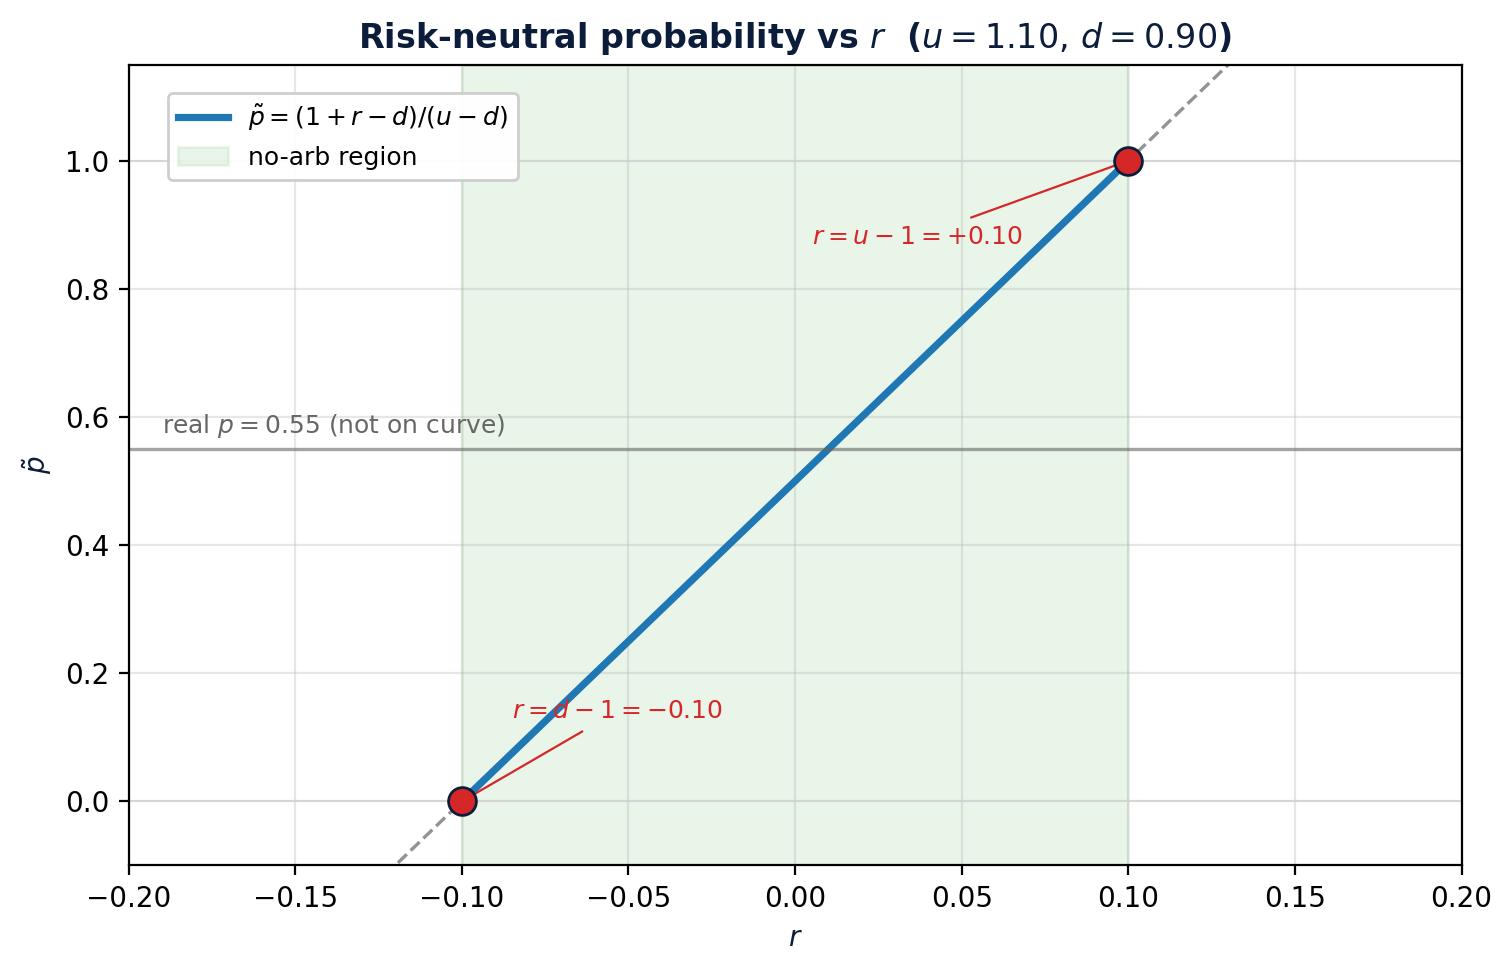
\includegraphics[keepaspectratio]{figures/ch01-tildep-vs-r.png}}
\caption{Risk-neutral probability \(\tilde p\) as a function of \(r\),
for fixed \(u=1.10, d=0.90\). The line crosses \(\tilde p=0\) at
\(r=-0.10\) (= \(d-1\)) and \(\tilde p=1\) at \(r=+0.10\) (= \(u-1\)).
Inside this range \(\tilde p\) is an honest probability; outside, the
market admits arbitrage. Real-world \(p=0.55\) is shaded in grey for
contrast --- \emph{it is not on this curve}.}
\end{figure}

\begin{figure}
\centering
\pandocbounded{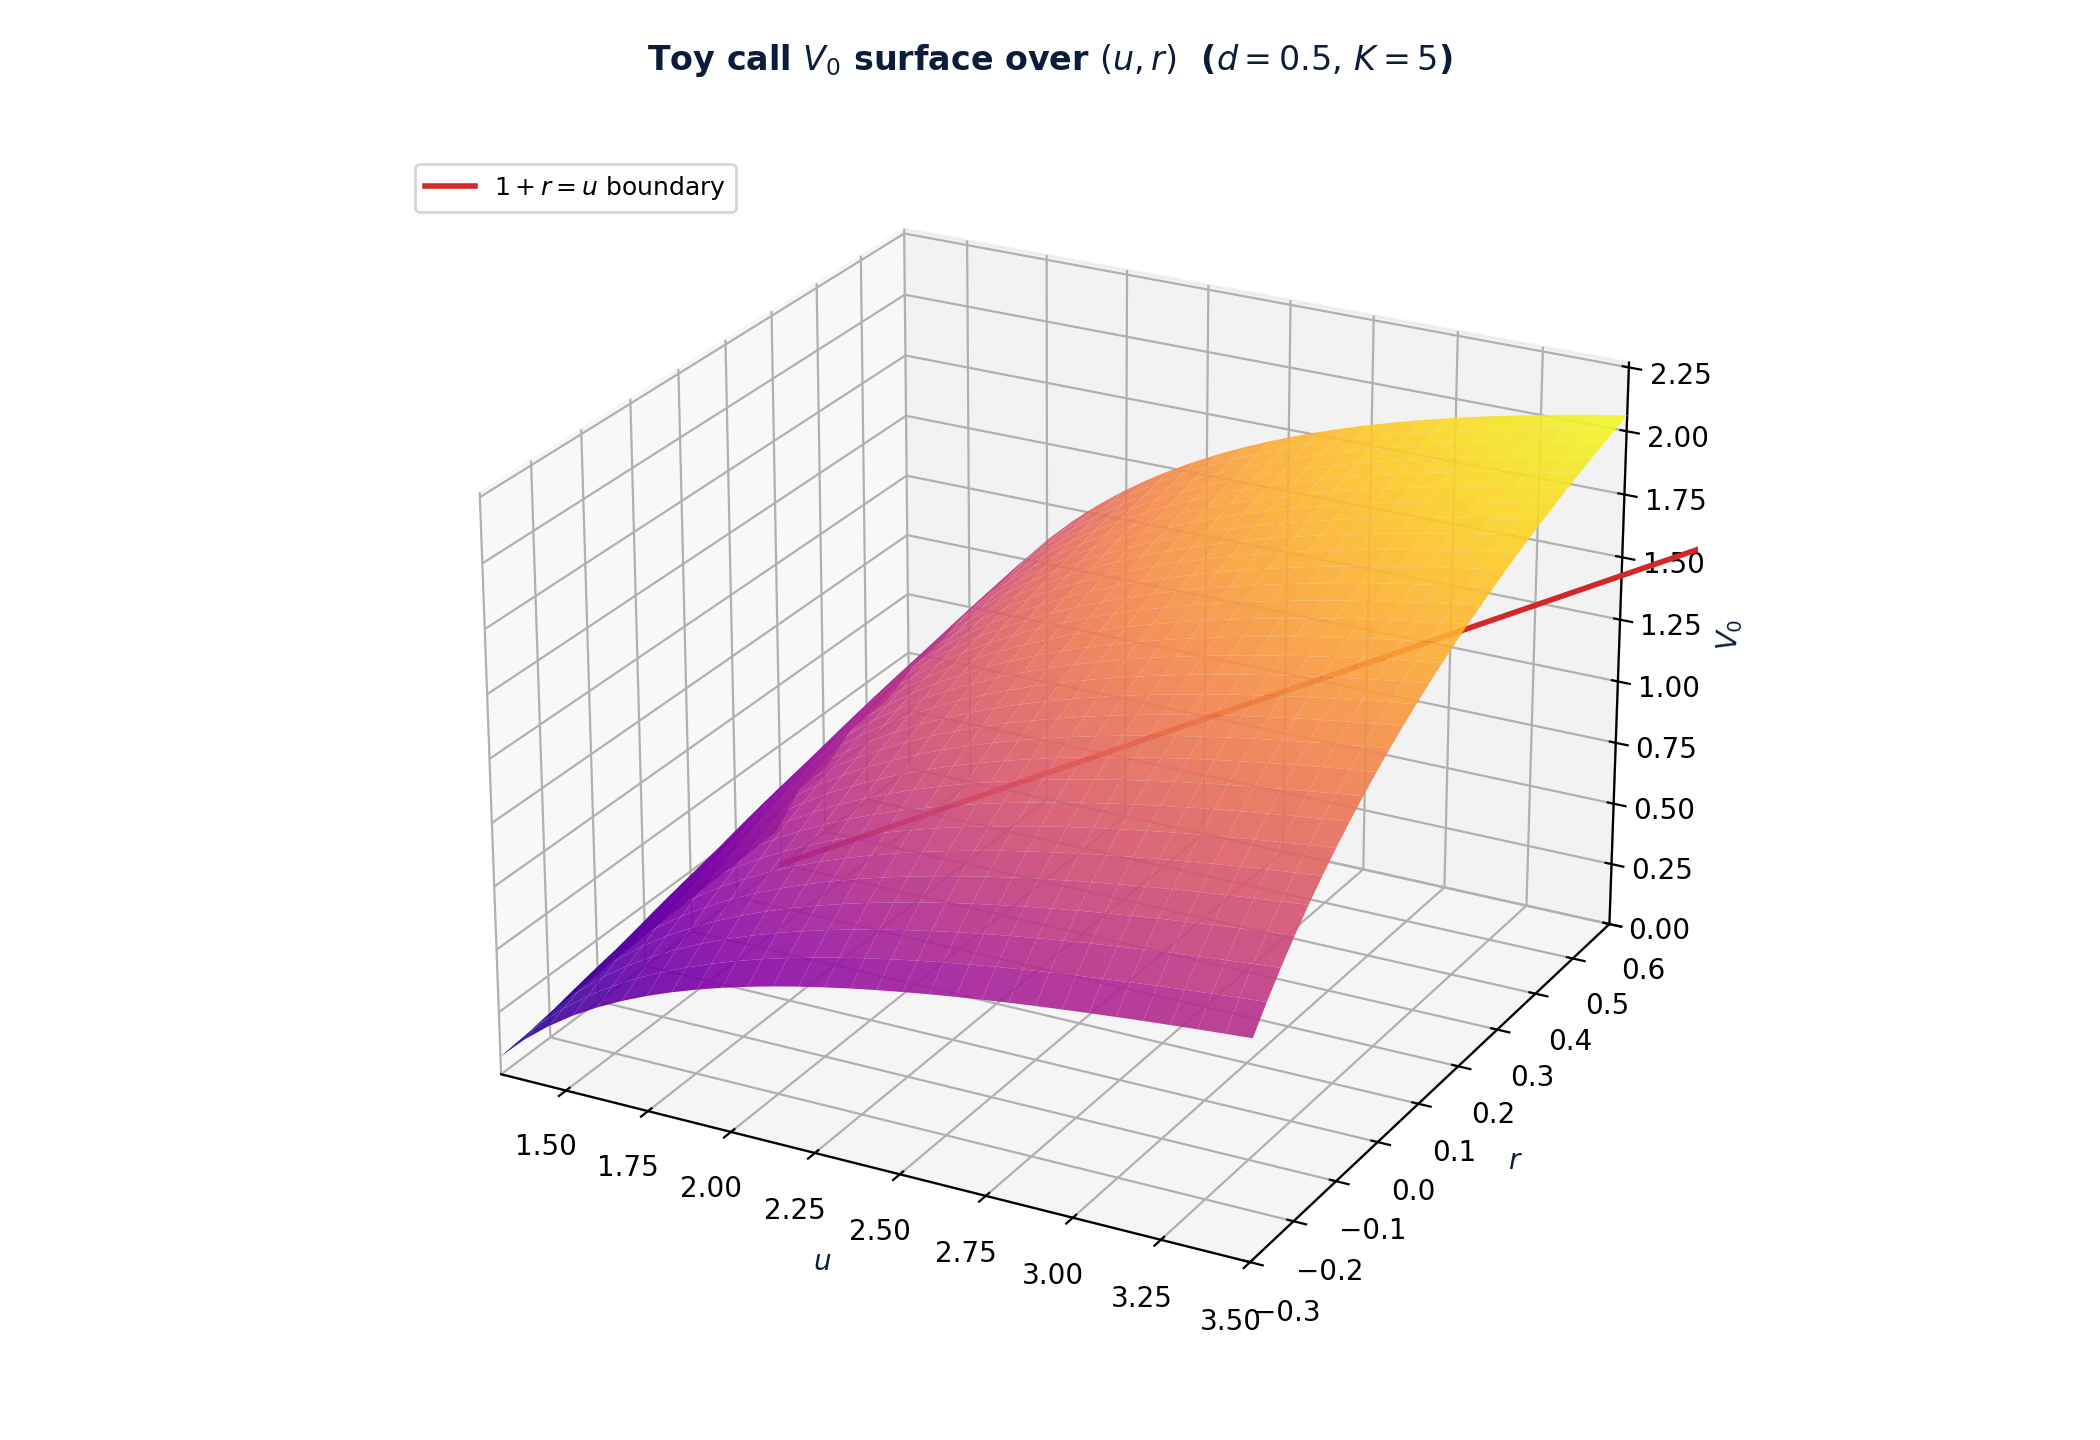
\includegraphics[keepaspectratio]{figures/ch01-call-surface-3d.png}}
\caption{3-D surface of ST call price \(V_0\) versus \((u,r)\), with
\(d=0.5\) and \(K=5\) fixed. The surface rises in both directions:
bigger \(u\) raises payoff, bigger \(r\) raises \(\tilde p\). The flat
colourful contours along the base show the boundary of the no-arbitrage
region (\(d<1+r<u\), here \(r\in(-0.5, u-1)\)).}
\end{figure}

\subsection{\texorpdfstring{1.5.7 \(\tilde p\)
table}{1.5.7 \textbackslash tilde p table}}\label{tilde-p-table}

\textbf{Table 1.6.} Ten \((u,d,r)\) triples and the resulting
\(\tilde p\). Broken rows (\(\tilde p\notin (0,1)\)) are flagged.

{\def\LTcaptype{none} % do not increment counter
\begin{table}[H]
\centering
\begin{tabular}{|r|r|r|r|l|}
\toprule
\(u\) & \(d\) & \(r\) & \(\tilde p\) & Verdict \\
\midrule



\(2.00\) & \(0.50\) & \(\phantom{-}0.25\) & \(0.5000\) & OK \\
\(1.10\) & \(0.90\) & \(\phantom{-}0.02\) & \(0.6000\) & OK \\
\(1.20\) & \(0.80\) & \(\phantom{-}0.05\) & \(0.6250\) & OK \\
\(1.05\) & \(0.95\) & \(\phantom{-}0.00\) & \(0.5000\) & OK \\
\(1.30\) & \(0.85\) & \(\phantom{-}0.10\) & \(0.5556\) & OK \\
\(1.50\) & \(0.80\) & \(\phantom{-}0.05\) & \(0.3571\) & OK \\
\(1.01\) & \(0.99\) & \(\phantom{-}0.02\) & \(1.5000\) &
\textbf{Broken} \\
\(1.20\) & \(1.05\) & \(\phantom{-}0.10\) & \(0.3333\) & OK \\
\(1.00\) & \(0.95\) & \(\phantom{-}0.00\) & \(1.0000\) & Boundary \\
\(1.10\) & \(0.90\) & \(\phantom{-}0.15\) & \(1.2500\) &
\textbf{Broken} \\
\bottomrule
\end{tabular}
\end{table}
}

\emph{Legend.} OK = \(\tilde p\in(0,1)\) (no arbitrage). \textbf{Broken}
= \(\tilde p\notin(0,1)\); bond dominates (\(1+r>u\)). Boundary =
\(d=1+r\) or \(1+r=u\) (degenerate). The ``OK (\(d<1+r<u\))'' row at
\((u,d,r)=(1.20,1.05,0.10)\) satisfies \(1.05<1.10<1.20\).

The two genuinely broken rows give \(\tilde p\) outside \((0,1)\) ---
\emph{not an honest probability}, confirming the no-arbitrage failure.

\subsection{1.5.8 Exercises}\label{exercises-15}

\begin{enumerate}
\def\labelenumi{\arabic{enumi}.}
\tightlist
\item
  Compute \(\tilde p\) for \(u=1.25, d=0.80, r=0.02\). \textbf{Answer:}
  \((1.02-0.80)/(1.25-0.80)=0.22/0.45=0.4889\).
\item
  Price a digital with \(K=4\) in ST. \textbf{Answer:} \(V_u=1\) (since
  \(8>4\)), \(V_d=0\) (since \(2<4\)). \(V_0=0.4\cdot 1=0.40\). Same as
  \(K=5\) here --- coincidence.
\item
  Price an option that pays \(\$1\) only when the stock goes \emph{down}
  (RL). \textbf{Answer:} \((0,1)\). \(V_0=0.4/1.02=0.3922\).
\end{enumerate}

\begin{center}\rule{0.5\linewidth}{0.5pt}\end{center}

\section{§1.6 Why the two routes give the same
number}\label{why-the-two-routes-give-the-same-number}

\textbf{Punchline.} Plug the closed-form \((\Delta,B)\) into
\(\Delta S_0+B\) and you get \((1/(1+r))[\tilde p V_u + \tilde q V_d]\)
by pure algebra. The two formulas are \emph{literally the same
expression}, written differently.

\textbf{Intuition.} Imagine two paths from your house to a friend's. One
winds through the woods (replication); the other takes the highway
(\(\tilde p\)). They end at the same friend. The algebra we did in
§1.5.1 is exactly the proof that both paths reach the same destination.
The replication route is \emph{constructive} --- it tells you the hedge.
The \(\tilde p\) route is \emph{computational} --- it just gives you the
price. In practice, traders use \(\tilde p\) to \emph{quote} prices and
\(\Delta\) to \emph{hedge}.

\subsection{1.6.1 The algebraic identity, line by
line}\label{the-algebraic-identity-line-by-line}

Recall:

\begin{itemize}
\tightlist
\item
  Replication: \(V_0^{\text{rep}} = \Delta S_0 + B\), with
  \(\Delta = (V_u-V_d)/((u-d)S_0)\) and
  \(B = (uV_d-dV_u)/((u-d)(1+r))\).
\item
  Risk-neutral:
  \(V_0^{\text{rn}} = (1/(1+r))[\tilde p V_u + \tilde q V_d]\), with
  \(\tilde p = ((1+r)-d)/(u-d)\) and \(\tilde q = (u-(1+r))/(u-d)\).
\end{itemize}

Step 1. Compute \(\Delta S_0\):

\[\Delta S_0 = \frac{V_u - V_d}{u-d}.\]

Step 2. Add \(B\):

\[\Delta S_0 + B = \frac{V_u-V_d}{u-d} + \frac{uV_d-dV_u}{(u-d)(1+r)}.\]

Step 3. Common denominator \((u-d)(1+r)\):

\[= \frac{(1+r)(V_u-V_d) + uV_d - dV_u}{(u-d)(1+r)} = \frac{V_u[(1+r)-d] + V_d[u-(1+r)]}{(u-d)(1+r)}.\]

Step 4. Factor out \(1/(1+r)\):

\[
\begin{aligned}
&= \frac{1}{1+r}\cdot\Big[V_u\cdot\frac{(1+r)-d}{u-d} + V_d\cdot\frac{u-(1+r)}{u-d}\Big] \\
&= \frac{1}{1+r}[\tilde p V_u + \tilde q V_d] \;=\; V_0^{\text{rn}}.
\end{aligned}
\]

Done.

\subsection{1.6.2 Line-by-line numerical
confirmations}\label{line-by-line-numerical-confirmations}

\textbf{Example 1.6.1 (ST call, \(K=5\)).} Replication:
\(\Delta=0.5, B=-0.8\), \(V_0=0.5(4)-0.8=1.20\). RN:
\((0.5\cdot 3+0.5\cdot 0)/1.25=1.5/1.25=1.20\). ✓

\textbf{Example 1.6.2 (RL put, \(K=100\)).} Replication:
\(-0.5(100)+53.9216=3.9216\). RN:
\((0.6\cdot 0+0.4\cdot 10)/1.02=4/1.02=3.9216\). ✓

\textbf{Example 1.6.3 (ST custom \((25,-5)\)).} Replication:
\(5(4)-12=8\). RN: \(0.4(25+(-5))=0.4(20)=8\). ✓

\textbf{Example 1.6.4 (ST forward \(K=5\)).} Replication: \(1(4)-4=0\).
RN: \(0.4(3-3)=0\). ✓

\textbf{Example 1.6.5 (RL straddle \(K=100\)).} Replication:
\(0(100)+9.8039=9.8039\). RN: \((0.6(10)+0.4(10))/1.02=10/1.02=9.8039\).
✓

\textbf{Example 1.6.6 (a mistyped formula --- counterexample).} Suppose
someone writes ``\(V_0 = (\tilde p V_u + (1-\tilde p)V_d) / r\)'' ---
missing the \(1+\). For ST call: \(0.5(3)/0.25 = 6\). That's wrong (off
by a factor of \(5\)). The point: discount factor is \(1/(1+r)\), not
\(1/r\); the latter would only be correct if \(r=1\) (a 100\% rate).

\subsection{1.6.3 Commutative diagram}\label{commutative-diagram}

\begin{figure}
\centering
\pandocbounded{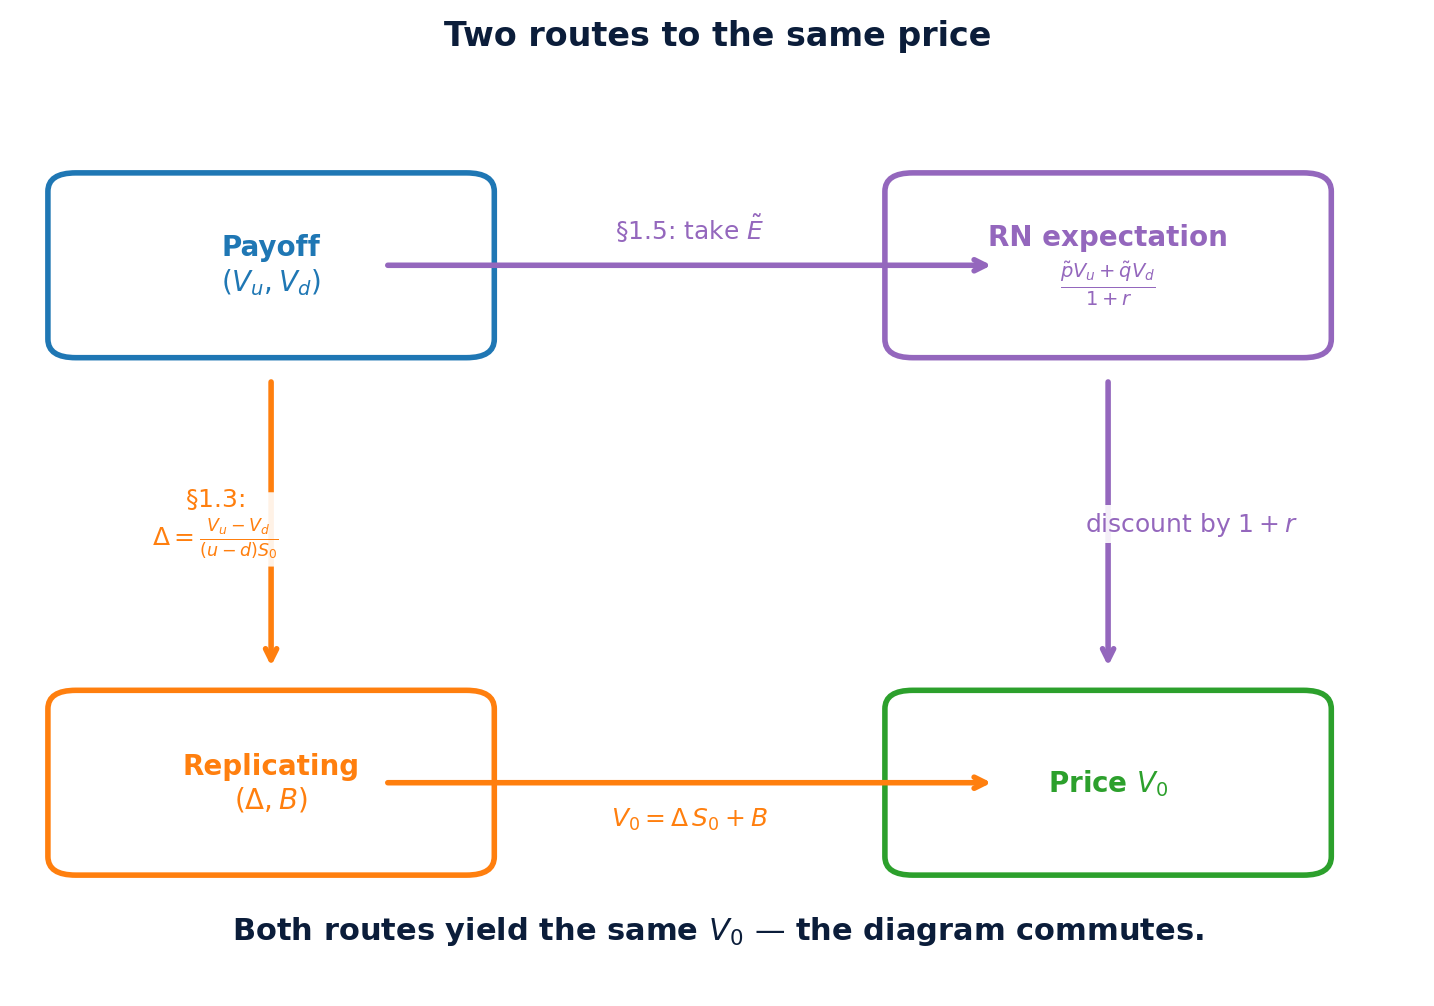
\includegraphics[keepaspectratio]{figures/ch01-commutative-diagram.png}}
\caption{Commutative diagram of the two pricing routes. Top-left node:
payoff \((V_u,V_d)\). Bottom-left: replicating portfolio \((\Delta,B)\)
via §0.11. Top-right: discounted RN expectation
\((\tilde p V_u + \tilde q V_d)/(1+r)\) via §1.5. Both routes end at
\(V_0\) (bottom-right). The arrow labels are the §1.3 formulas and the
§1.5 formula. The diagram commutes --- both compositions yield the same
answer.}
\end{figure}

\subsection{1.6.4 Algebra steps as a
table}\label{algebra-steps-as-a-table}

\textbf{Table 1.7.} The four steps of the §1.6.1 identity, applied to
the ST call.

{\def\LTcaptype{none} % do not increment counter
\begin{table}[H]
\centering
\begin{tabular}{|l|l|r|}
\toprule
Step & Symbolic & Number \\
\midrule



1: \(\Delta S_0\) & \(\tfrac{V_u-V_d}{u-d}\) & \(2.000\) \\
2: \(\Delta S_0+B\) & step 1 \(+\,\tfrac{uV_d-dV_u}{(u-d)(1+r)}\) &
\(1.200\) \\
3: common den. & combine: see line below & \(1.200\) \\
4: factor \(\tilde p\) & \(\tfrac{1}{1+r}(\tilde p V_u+\tilde q V_d)\) &
\(1.200\) \\
\bottomrule
\end{tabular}
\end{table}
}

Row 1: \((3-0)/1.5 = 2.0\). Row 2:
\(2.0 + (2\cdot 0 - 0.5\cdot 3)/1.875 = 2.0 + (-1.5)/1.875 = 2.0 - 0.8 = 1.2\).
Row 3 (common denominator \((u-d)(1+r)\)):
\(\tfrac{(1+r)(V_u-V_d) + uV_d - dV_u}{(u-d)(1+r)} = (1.25\cdot 3 - 0.5\cdot 3)/1.875 = 2.25/1.875 = 1.2\).
Row 4: \(0.8 \cdot (0.5 \cdot 3 + 0.5 \cdot 0) = 0.8 \cdot 1.5 = 1.2\).

\subsection{1.6.5 Exercises}\label{exercises-16}

\begin{enumerate}
\def\labelenumi{\arabic{enumi}.}
\tightlist
\item
  Verify Example 1.6.1 by replication line by line on the RL call.
  \textbf{Answer:} \(\Delta S_0=0.5(100)=50\). \(B=-44.1176\). Sum
  \(=5.8824\).
\item
  Use \(\tilde p\) to price RL forward \(K=102\). \textbf{Answer:}
  \((0.6(8)+0.4(-12))/1.02=(4.8-4.8)/1.02=0\). ✓
\item
  Show that the price of the asset-or-nothing in ST equals
  \(0.4(8) = 3.20\) via \(\tilde p\).
\end{enumerate}

\begin{center}\rule{0.5\linewidth}{0.5pt}\end{center}

\section{\texorpdfstring{§1.7 Why ``risk-neutral'': expected return =
\(r\) under
\(\tilde{\mathbb P}\)}{§1.7 Why ``risk-neutral'': expected return = r under \textbackslash tilde\{\textbackslash mathbb P\}}}\label{why-risk-neutral-expected-return-r-under-tildemathbb-p}

\textbf{Punchline.} Under the risk-neutral probability \(\tilde p\), the
stock has expected one-period gross return \(1+r\) --- \emph{the same as
the bond}. Discounted prices are martingales. Under the real probability
\(p\), by contrast, the stock has expected return \emph{above} \(r\) (a
``risk premium'').

\textbf{Intuition.} Asking ``what probability would make the stock's
expected return equal \(r\)?'' gives you a system of one equation in one
unknown --- the answer is exactly \(\tilde p\). So \(\tilde p\) is the
unique probability under which buying the stock is no better than buying
the bond. In \emph{that} world, no one cares about risk (everything
earns \(r\)). The actual world's probability \(p\) may be higher (giving
the stock a positive risk premium) or different in some other way; it
doesn't matter for pricing.

\subsection{1.7.1 The martingale
identity}\label{the-martingale-identity}

Compute \(\widetilde{\mathbb E}[S_1]\):

\[\widetilde{\mathbb E}[S_1] = \tilde p\, uS_0 + (1-\tilde p)\, dS_0 = S_0[\tilde p u + (1-\tilde p)d].\]

Substitute \(\tilde p = ((1+r)-d)/(u-d)\):

\[
\begin{aligned}
\tilde p\, u + (1-\tilde p)\, d
&= \frac{\bigl((1+r) - d\bigr)\,u \;+\; \bigl(u - (1+r)\bigr)\,d}{u-d} \\
&= \frac{u(1+r) - ud + ud - d(1+r)}{u-d} \\
&= \frac{(1+r)(u-d)}{u-d} \\
&= 1+r.
\end{aligned}
\]

So \(\widetilde{\mathbb E}[S_1] = (1+r)S_0\). The discounted stock
\(S_1/(1+r)\) has expectation \(S_0\) --- a \emph{martingale} (one-step
martingale: today's value equals tomorrow's risk-neutral expectation).

\subsection{1.7.2 The real-world return
differs}\label{the-real-world-return-differs}

Pick a real-world probability \(p\) (different from \(\tilde p\) in
general). Then

\[\mathbb E[S_1] = puS_0 + (1-p)dS_0 = S_0[pu+(1-p)d].\]

This equals \((1+r)S_0\) iff \(p = \tilde p\). For any other \(p\),
there's a gap.

\textbf{Example 1.7.1 (ST, \(p=0.7\)).}
\(\mathbb E[S_1]/S_0 = 0.7(2)+0.3(0.5) = 1.55\). So real expected return
is \(55\%\) --- much higher than \(r=25\%\). \emph{Risk premium}:
\(55\%-25\%=30\%\).

\textbf{Example 1.7.2 (RL, \(p=0.55\)).}
\(\mathbb E[S_1]/S_0 = 0.55(1.10)+0.45(0.90) = 0.605+0.405=1.01\). Real
expected return \(1\%\), below the bond's \(2\%\)! That's a
\emph{negative} risk premium --- investors would be irrational to hold
this stock voluntarily. Either \(p\) is wrong, or the stock has some
other compensation (e.g., it's a hedge).

\textbf{Example 1.7.3 (RL, \(p=0.65\)).}
\(\mathbb E[S_1]/S_0 = 0.65(1.10)+0.35(0.90) = 0.715+0.315=1.03\). Real
expected return \(3\%\), risk premium \(1\%\) over the bond.

\textbf{Example 1.7.4 (ST under \(\tilde p=0.5\)).}
\(\widetilde{\mathbb E}[S_1]/S_0 = 0.5(2)+0.5(0.5)=1.25=1+r\). ✓

\textbf{Example 1.7.5 (RL under \(\tilde p=0.6\)).}
\(0.6(1.10)+0.4(0.90)=0.66+0.36=1.02=1+r\). ✓

\subsection{1.7.3 The call's risk-neutral expected
return}\label{the-calls-risk-neutral-expected-return}

\textbf{Example 1.7.6 (ST call expected return under \(\tilde p\)).}
Price today \(1.20\). Time-1 payoff: \(3\) with prob \(\tilde p=0.5\),
\(0\) with prob \(0.5\). Expected payoff \(1.5\). Expected gross return
\(1.5/1.20 = 1.25 = 1+r\). ✓

\textbf{Example 1.7.7 (ST call under real \(p=0.7\)).} Expected payoff
\(0.7(3) = 2.10\). Expected gross return \(2.10/1.20 = 1.75\). \emph{Far
higher than the bond}. Calls are levered bets; under any sensible
real-world \(p\) they earn enormous expected returns. (And lose money
most of the time, of course --- that's the high-variance side.)

\textbf{Example 1.7.8 (bond is a trivial martingale).} Bond pays \(1+r\)
in both states.
\(\widetilde{\mathbb E}[\text{bond}_1]/(1+r) = (1+r)/(1+r) = 1 = \text{bond}_0\).
✓

\subsection{1.7.4 Side-by-side trees and bar
chart}\label{side-by-side-trees-and-bar-chart}

\begin{figure}
\centering
\pandocbounded{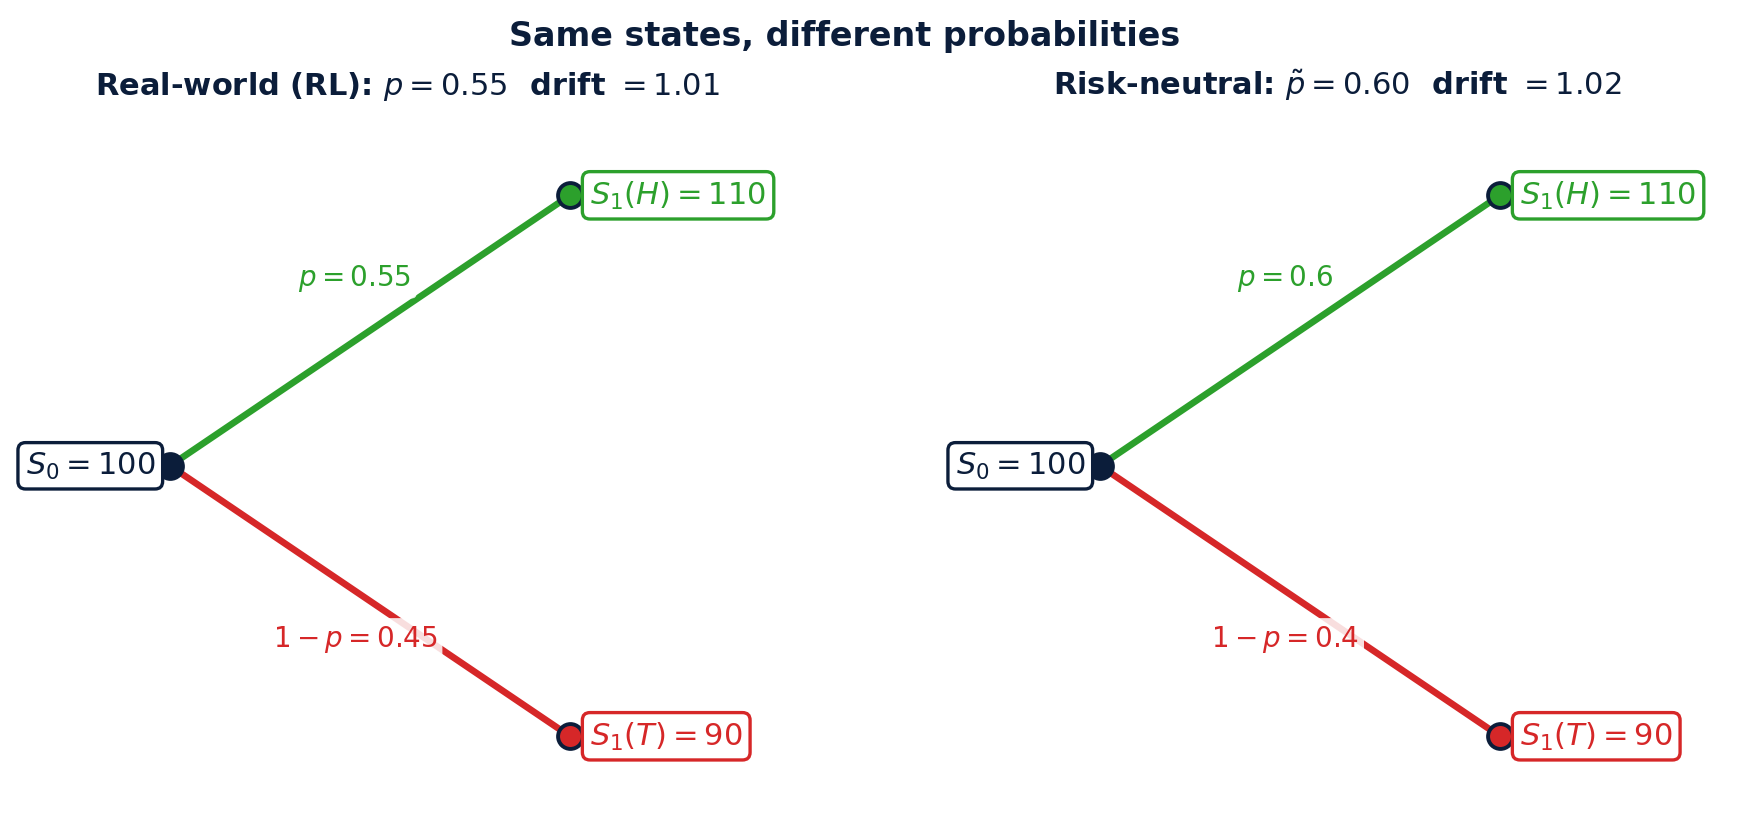
\includegraphics[keepaspectratio]{figures/ch01-real-vs-rn-trees.png}}
\caption{Real-world tree (left, \(p=0.55\) for RL) and risk-neutral tree
(right, \(\tilde p=0.6\)). The probabilities on the edges differ, but
the state values \(\{uS_0, dS_0\}\) are the same. Under the real
probability the drift is \(1.01\); under RN it's \(1.02\). The drift
adjustment from real to RN is exactly the risk premium subtraction.}
\end{figure}

\begin{figure}
\centering
\pandocbounded{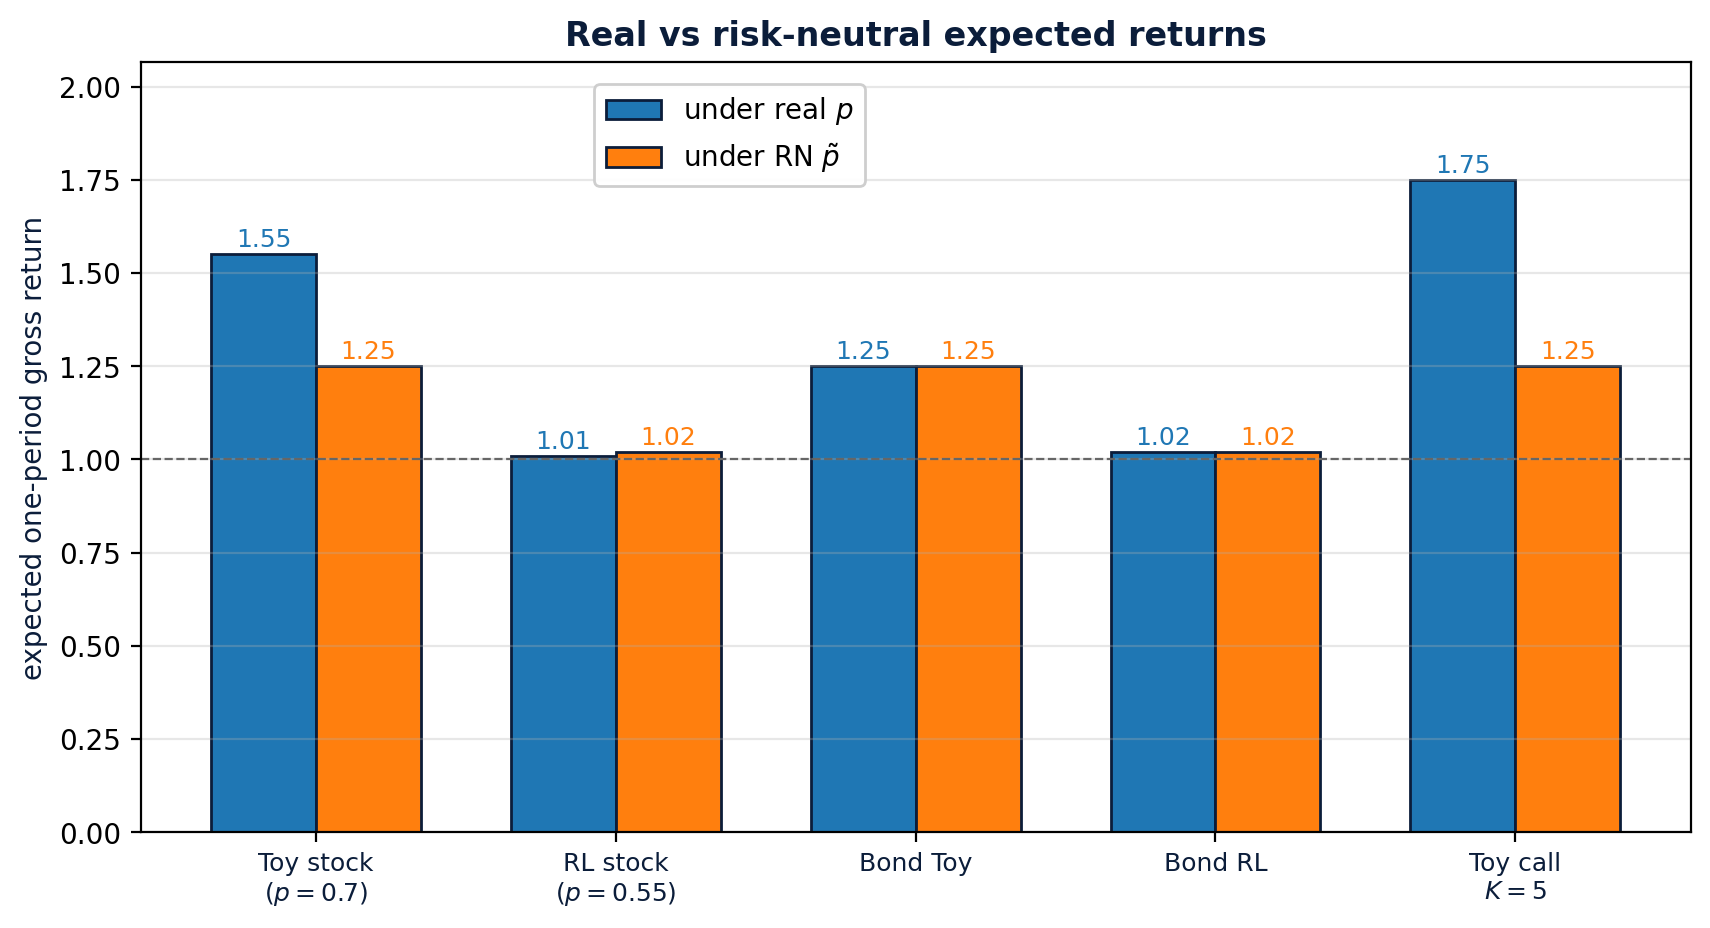
\includegraphics[keepaspectratio]{figures/ch01-returns-bars.png}}
\caption{Bar chart of expected one-period gross returns. Under real
\(p=0.55\), RL stock returns \(1.01\), ST stock returns (\(p=0.7\))
\(1.55\). Under RN, both stocks return \(1+r\) (= \(1.02\) and \(1.25\)
respectively). Bonds always return \(1+r\). The call returns \(1+r\)
under RN but is wildly higher under real \(p\).}
\end{figure}

\subsection{\texorpdfstring{1.7.5 Asset returns under \(\mathbb P\) vs
\(\tilde{\mathbb P}\)}{1.7.5 Asset returns under \textbackslash mathbb P vs \textbackslash tilde\{\textbackslash mathbb P\}}}\label{asset-returns-under-mathbb-p-vs-tildemathbb-p}

\textbf{Table 1.8.} Expected gross returns in the two probability
measures.

{\def\LTcaptype{none} % do not increment counter
\begin{table}[H]
\centering
\begin{tabular}{|l|r|r|}
\toprule
Asset & \(\mathbb E[\cdot]\) under \(\mathbb P\) & \(\widetilde{\mathbb E}[\cdot]\) under \(\tilde{\mathbb P}\) \\
\midrule



ST stock & \(1.55\) & \(1.25\) \\
ST bond & \(1.25\) & \(1.25\) \\
ST call & \(1.75\) & \(1.25\) \\
RL stock & \(1.01\) & \(1.02\) \\
RL bond & \(1.02\) & \(1.02\) \\
RL call & \(0.935\) & \(1.02\) \\
\bottomrule
\end{tabular}
\end{table}
}

\emph{Notes.} ST entries use \(p=0.7\); RL entries use \(p=0.55\). RL
call: \(\mathbb E[V_1] = 0.55(10) + 0.45(0) = 5.5\); gross return
\(5.5/5.8824 = 0.935\).

Note the \emph{RL call under \(p=0.55\) has expected return below 1!}
--- under such a low \(p\) the call mostly expires worthless. This is
consistent with \(p<\tilde p=0.6\).

\subsection{1.7.6 Exercises}\label{exercises-17}

\begin{enumerate}
\def\labelenumi{\arabic{enumi}.}
\tightlist
\item
  In ST with \(p=0.6\), find expected stock return. \textbf{Answer:}
  \(0.6(2)+0.4(0.5)=1.40\), so \(40\%\).
\item
  In RL, what \(p\) gives the stock a real return of exactly \(5\%\)?
  \textbf{Answer:}
  \(1.10p+0.90(1-p)=1.05 \Rightarrow 0.20p+0.90=1.05 \Rightarrow p=0.75\).
\item
  Verify the put's expected return under \(\tilde p\) in ST equals
  \(1.25\). \textbf{Answer:} \(\mathbb E[V_1]=0.5(0)+0.5(3)=1.5\).
  \(V_0=1.20\). Ratio \(1.25\). ✓
\end{enumerate}

\begin{center}\rule{0.5\linewidth}{0.5pt}\end{center}

\section{§1.8 Worked menagerie: a tour of one-period
derivatives}\label{worked-menagerie-a-tour-of-one-period-derivatives}

\textbf{Punchline.} Every ``vanilla'' derivative reduces to a payoff
pair \((V_u,V_d)\) and is priced by the same single formula. This
section is a tour through nine derivatives across both markets --- call,
put, digital cash, digital asset, forward, straddle, risk-reversal,
power, capped call.

\textbf{Intuition.} Once the machinery is built, the work is just
plugging in payoffs and turning a crank. The instruments differ by their
\emph{payoff structure}, not by the pricing method. Each one gives a
different shape of payoff diagram; understanding those shapes is most of
the trader-intuition you need.

\subsection{1.8.1 Payoff diagrams}\label{payoff-diagrams}

\begin{figure}
\centering
\pandocbounded{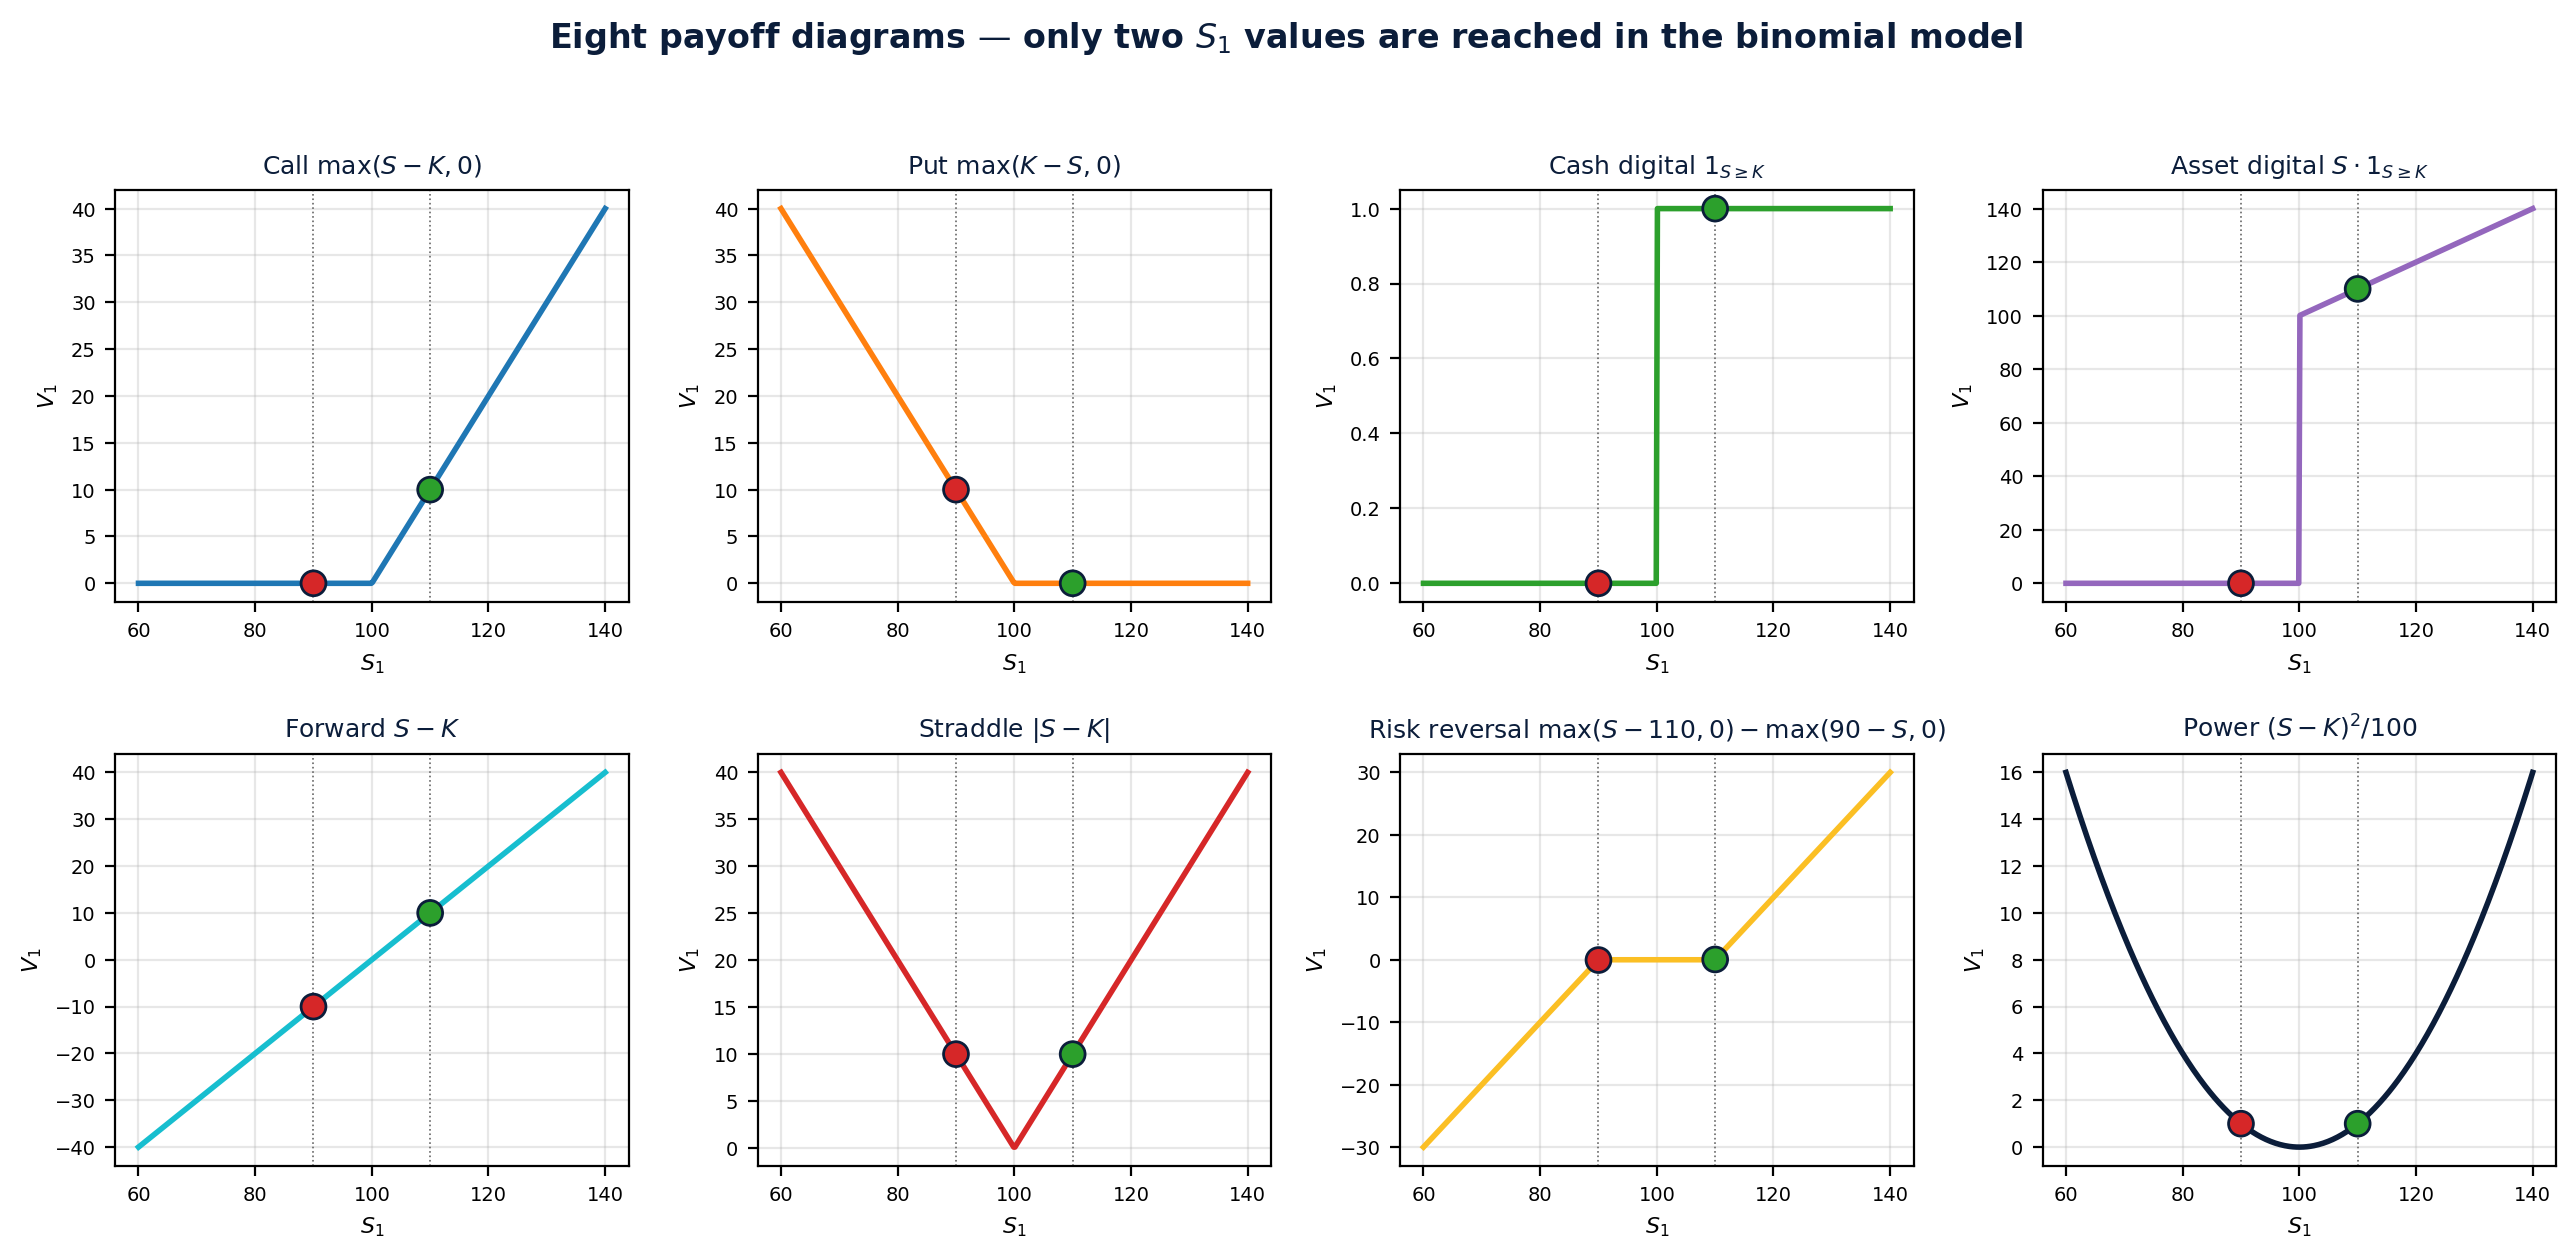
\includegraphics[keepaspectratio]{figures/ch01-payoff-strip.png}}
\caption{Eight payoff diagrams on a single strip: (1) call, (2) put, (3)
cash digital, (4) asset digital, (5) forward, (6) straddle, (7)
risk-reversal, (8) power option (quadratic). Each is plotted as \(V_1\)
versus \(S_1\) on a continuous axis (even though in our model only two
points of that axis are reached). The two binomial outcomes are marked
as colourful dots.}
\end{figure}

\subsection{1.8.2 Each derivative priced in both
worlds}\label{each-derivative-priced-in-both-worlds}

\textbf{Example 1.8.1 (Call, ST).} Already computed: \(V_0=1.20\).

\textbf{Example 1.8.2 (Call, RL).} Already computed: \(V_0=5.8824\).

\textbf{Example 1.8.3 (Put, ST).} \(1.20\).

\textbf{Example 1.8.4 (Put, RL).} \(3.9216\).

\textbf{Example 1.8.5 (Cash digital, ST, \(K=5\)).} \(V_0=0.40\).

\textbf{Example 1.8.6 (Cash digital, RL, \(K=100\)).} \(V_0=0.5882\).

\textbf{Example 1.8.7 (Asset digital, ST, \(K=5\)).} \(V_0=3.20\).

\textbf{Example 1.8.8 (Asset digital, RL, \(K=100\)).} \(V_u=110\)
(since \(110>100\)), \(V_d=0\) (since \(90<100\)).
\(V_0=(0.6\cdot 110+0)/1.02=66/1.02=64.706\).

Note: \$\text{Asset digital} - K\cdot\text{Cash digital} = \$ Call.
(\(64.706 - 100(0.5882) = 64.706 - 58.82 = 5.88\), matching the call.) ✓

\textbf{Example 1.8.9 (Forward, ST, \(K=5\)).} \(V_0=0\). Fair forward
\(F=(1+r)S_0=5\).

\textbf{Example 1.8.10 (Forward, RL, \(K=100\)).} \(V_0=1.9608\). Fair
forward \(F=102\).

\textbf{Example 1.8.11 (Straddle, ST, \(K=4\)).} \(V_0=2.40\).

\textbf{Example 1.8.12 (Straddle, RL, \(K=100\)).} \(V_0=9.8039\). Same
as discounted certain payoff because the straddle pays \(\$10\) in
\emph{both} states.

\textbf{Example 1.8.13 (Risk-reversal, ST, \(K_C=K_P=5\)).} Long call,
short put: \((V_u,V_d)=(3,0)-(0,3)=(3,-3)\). Same as the forward.
\(V_0=0\).

\textbf{Example 1.8.14 (Risk-reversal, RL, \(K_C=K_P=100\)).}
\((10,0)-(0,10)=(10,-10)\). \(V_0=1.9608\) (= forward at \(K=100\)).

\textbf{Example 1.8.15 (Power option, ST, exp 2).} \(V_0=27.20\).

\textbf{Example 1.8.16 (Power option, RL, exp 2).} \(V_0=10294.12\).

\textbf{Example 1.8.17 (Capped call, ST, \(K=4, C=6\)).} \(V_0=0.80\).

\textbf{Example 1.8.18 (Capped call, RL, \(K=100, C=105\)).}
\(V_0=2.9412\).

\subsection{1.8.3 Master menagerie table}\label{master-menagerie-table}

\textbf{Table 1.9.} Master menagerie --- prices in ST and RL.

{\def\LTcaptype{none} % do not increment counter
\begin{table}[H]
\centering
\begin{tabular}{|l|r|r|}
\toprule
Derivative & \(V_0\) (ST) & \(V_0\) (RL) \\
\midrule



Call (\(K=5\) / \(K=100\)) & \(\phantom{00}1.200\) &
\(\phantom{0000}5.882\) \\
Put (same) & \(\phantom{00}1.200\) & \(\phantom{0000}3.922\) \\
Cash digital & \(\phantom{00}0.400\) & \(\phantom{0000}0.588\) \\
Asset digital & \(\phantom{00}3.200\) & \(\phantom{000}64.706\) \\
Forward (ATM, \(K_F=5/100\)) & \(\phantom{00}0.000\) &
\(\phantom{0000}1.961\) \\
Straddle (ATM) & \(\phantom{00}2.400\) & \(\phantom{0000}9.804\) \\
Risk-reversal (ATM) & \(\phantom{00}0.000\) & \(\phantom{0000}1.961\) \\
Power option (exp 2) & \(27.200\) & \(10294.120\) \\
Capped call & \(\phantom{00}0.800\) & \(\phantom{0000}2.941\) \\
\bottomrule
\end{tabular}
\end{table}
}

\subsection{1.8.4 3-D menagerie price
plot}\label{d-menagerie-price-plot}

\begin{figure}
\centering
\pandocbounded{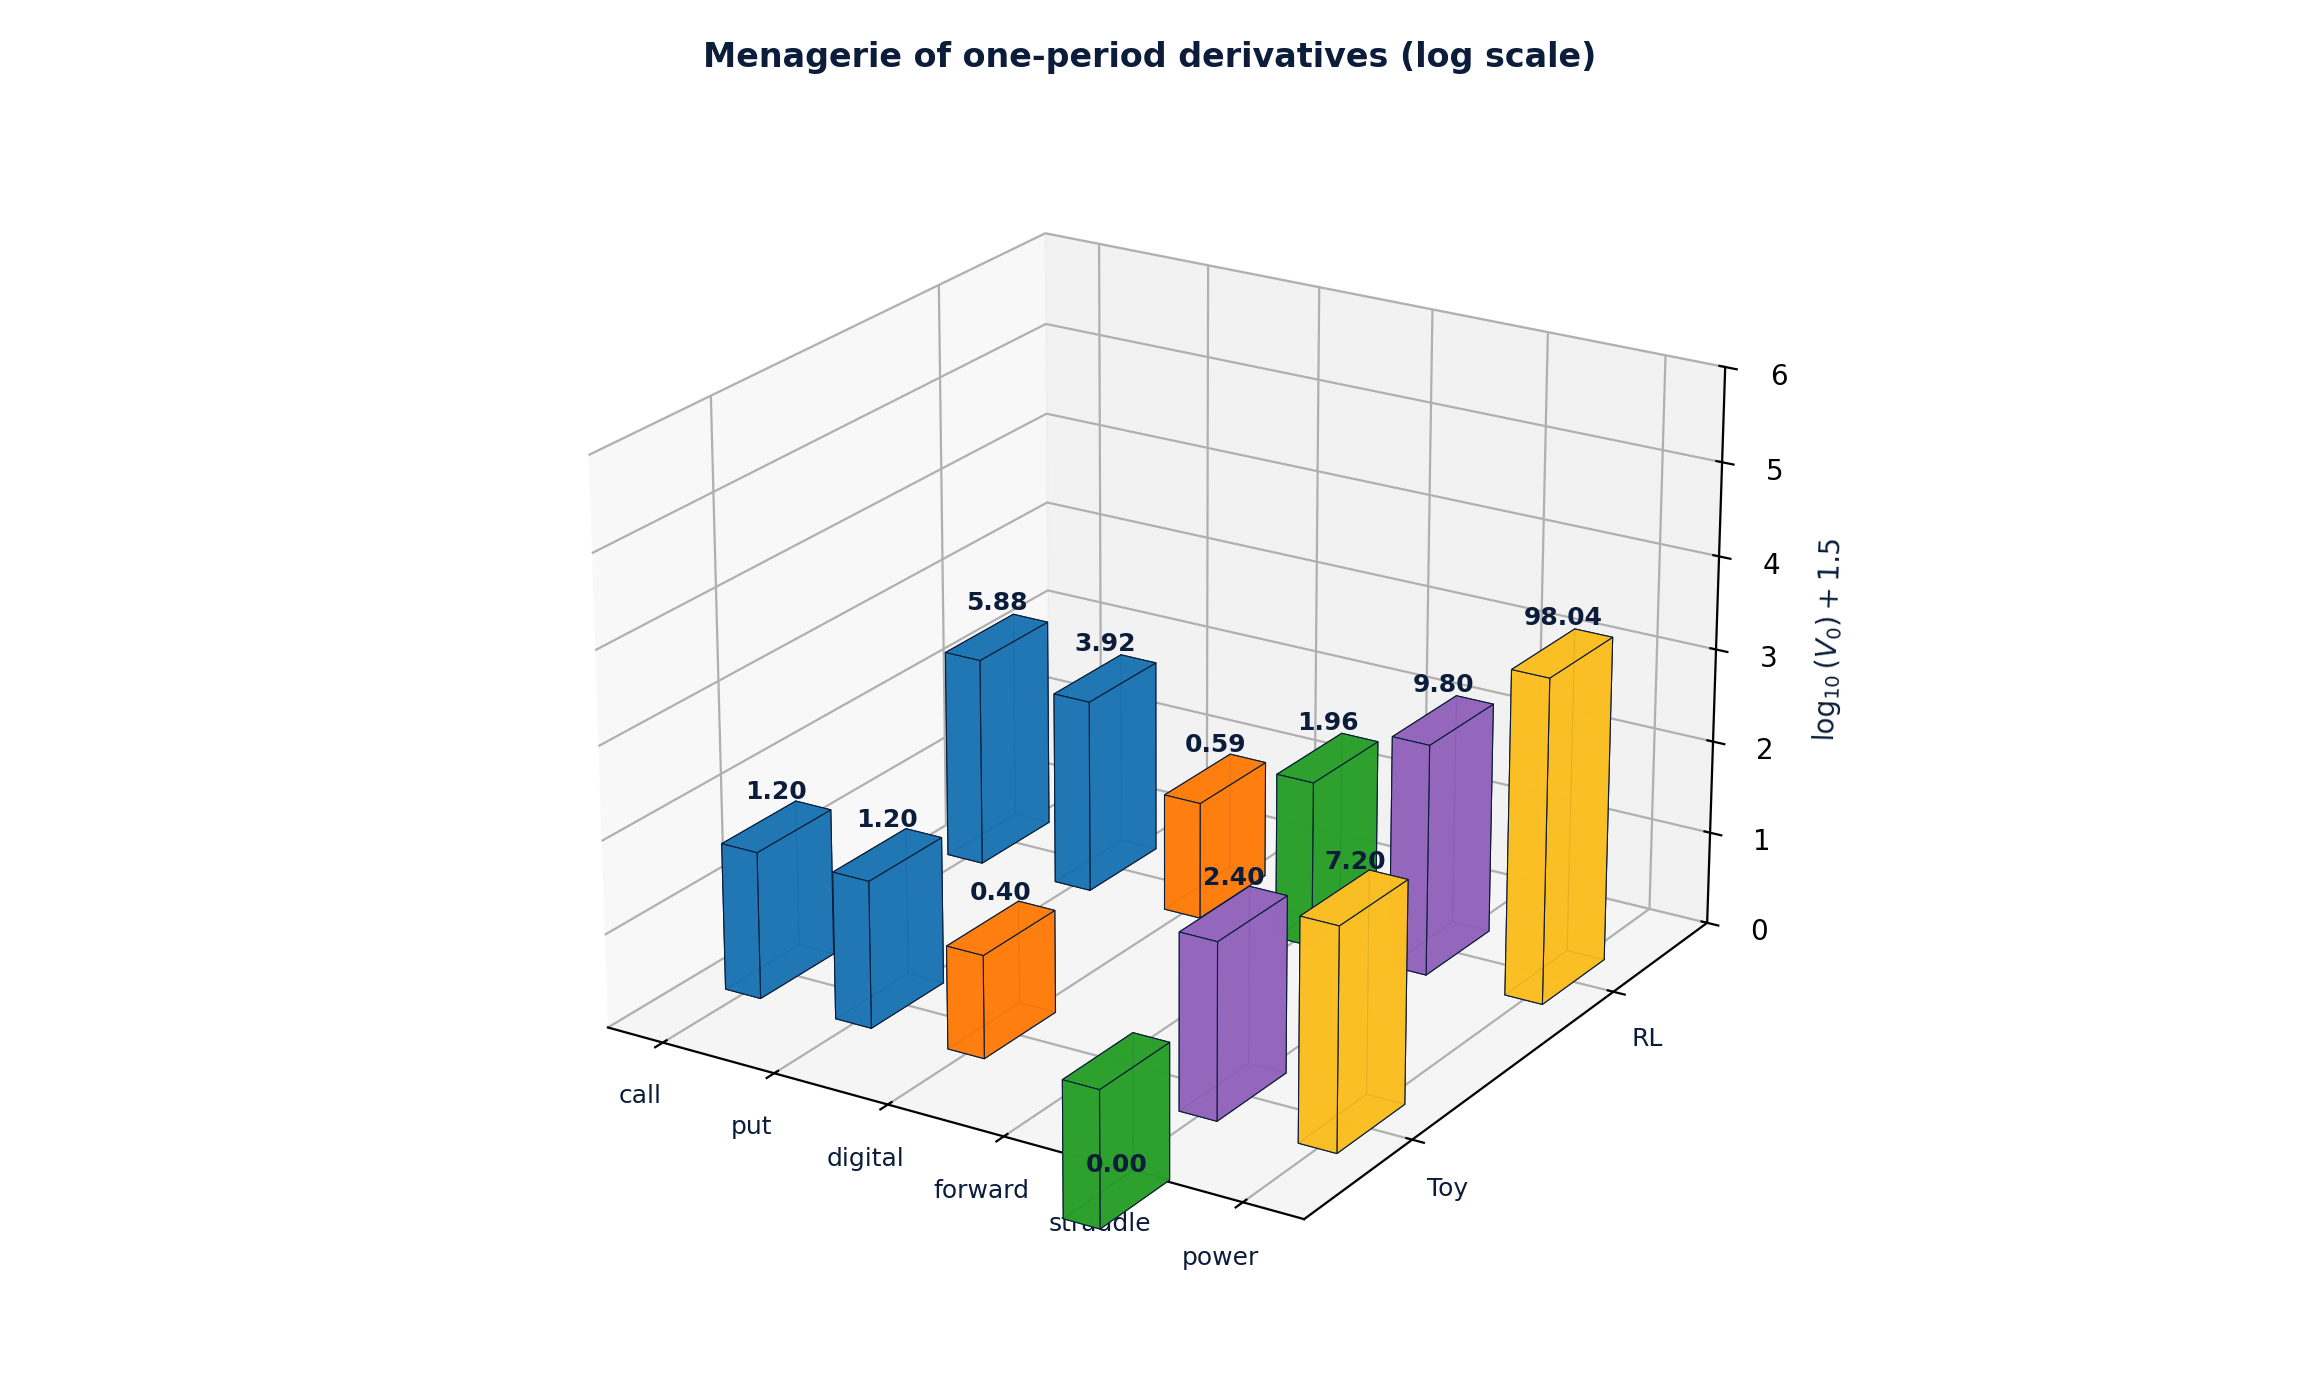
\includegraphics[keepaspectratio]{figures/ch01-menagerie-3d.png}}
\caption{3-D bar plot: derivative type along the \(x\)-axis, parameter
set (ST or RL) along the \(y\)-axis, price \(V_0\) along the \(z\)-axis
(log scale to accommodate the power option's \(10000\)). Bars are
colour-coded by derivative class --- calls/puts blue, digitals orange,
forwards green, straddles purple, others gold. The ST world is
consistently cheaper because \(S_0\) is smaller; RL prices scale roughly
proportionally to \(S_0\).}
\end{figure}

\subsection{1.8.5 Exercises}\label{exercises-18}

\begin{enumerate}
\def\labelenumi{\arabic{enumi}.}
\tightlist
\item
  Price a straddle struck at \(K=5\) in ST. \textbf{Answer:}
  \(V_u=|8-5|=3, V_d=|2-5|=3\). \(V_0=0.4(6)=2.40\). Same as \(K=4\)
  straddle? Indeed: as long as \(K\) is between \(d S_0\) and \(u S_0\),
  the straddle pays \(|S_1-K|\) which moves linearly across \(K\) but
  the sum \(V_u+V_d=(uS_0-K)+(K-dS_0)=(u-d)S_0\) is \emph{independent of
  \(K\)}. So all straddles with \(K\in[dS_0,uS_0]\) cost the same:
  \(0.4(u-d)S_0=0.4(6)=2.40\).
\item
  Price a capped call in RL with \(K=95, C=110\). \textbf{Answer:} Call
  payoff capped at \(C-K=15\): \(V_u=\min(\max(110-95,0),15)=15\);
  \(V_d=\min(\max(90-95,0),15)=0\).
  \(V_0=(0.6\cdot 15)/1.02=9/1.02=8.824\).
\item
  Show power option ST exp 3. \textbf{Answer:}
  \(V_u=8^3=512, V_d=2^3=8\). \(V_0=0.4(520)=208\).
\end{enumerate}

\begin{center}\rule{0.5\linewidth}{0.5pt}\end{center}

\section{§1.9 Put--call parity}\label{putcall-parity}

\textbf{Punchline.} For European call and put with the same strike \(K\)
and expiry,

\[\boxed{C_0 - P_0 \;=\; S_0 - \dfrac{K}{1+r}.}\]

This is a \emph{model-free} identity --- it doesn't depend on \(u, d\),
or \(\tilde p\), only on no-arbitrage.

\textbf{Intuition.} Look at the payoffs at \(t=1\):

\begin{itemize}
\tightlist
\item
  Call: \(\max(S_1-K,0)\)
\item
  Put: \(\max(K-S_1,0)\)
\item
  Call − Put = \(\max(S_1-K,0)-\max(K-S_1,0) = S_1-K\) (always! ---
  quick check: if \(S_1\ge K\), call − put \(= (S_1-K)-0=S_1-K\); if
  \(S_1<K\), call − put \(= 0-(K-S_1)=S_1-K\)).
\end{itemize}

So ``long call, short put'' is the same payoff as ``long forward struck
at \(K\)''. Both must cost the same today. The forward struck at \(K\)
costs \(S_0 - K/(1+r)\) (by §1.3.4 logic), giving the parity.

\subsection{1.9.1 Derivation from
no-arbitrage}\label{derivation-from-no-arbitrage}

The portfolio ``long one share, short \(K/(1+r)\) in bonds'' has \(t=0\)
cost \(S_0 - K/(1+r)\) and \(t=1\) value \(S_1 - K\) in either state.

The portfolio ``long one call, short one put'' has \(t=0\) cost
\(C_0-P_0\) and \(t=1\) value \(\max(S_1-K,0)-\max(K-S_1,0)=S_1-K\).

Same \(t=1\) payoffs, so same \(t=0\) prices:
\(C_0 - P_0 = S_0 - K/(1+r)\). □

\subsection{1.9.2 Worked verifications}\label{worked-verifications-1}

\textbf{Example 1.9.1 (ST, \(K=5\)).} \(C_0=P_0=1.20\), so
\(C_0-P_0=0\). \(S_0-K/(1+r) = 4 - 5/1.25 = 4 - 4 = 0\). ✓

\textbf{Example 1.9.2 (RL, \(K=100\)).} \(C_0=5.8824, P_0=3.9216\).
\(C_0-P_0=1.9608\).
\(S_0-K/(1+r) = 100 - 100/1.02 = 100 - 98.0392 = 1.9608\). ✓

\textbf{Example 1.9.3 (RL, \(K=95\)).} \(C_u=\max(110-95,0)=15\),
\(C_d=\max(90-95,0)=0\), \(C_0=(0.6\cdot 15)/1.02 = 8.8235\). \(P_u=0\),
\(P_d=\max(95-90,0)=5\), \(P_0=(0.4\cdot 5)/1.02 = 1.9608\).
\(C-P=6.8627\). RHS: \(100-95/1.02=100-93.1373=6.8627\). ✓

\textbf{Example 1.9.4 (RL, \(K=105\)).} \(C_u=5, C_d=0, C_0=2.9412\).
\(P_u=0, P_d=15, P_0=5.8824\). \(C-P=-2.9412\). RHS:
\(100-105/1.02=100-102.9412=-2.9412\). ✓

\textbf{Example 1.9.5 (Parity arb).} Suppose RL call is \(5.50\) (cheap)
but put is \(3.92\) (correct). Then \(C-P=1.58 < 1.96 =\) RHS.
Arbitrage: buy call (\(-5.50\)), sell put (\(+3.92\)), short stock
(\(+100\)), lend \(98.0392\) (\(-98.0392\)). Net cash:
\(-5.50+3.92+100-98.0392 = +0.3808\). At \(t=1\), call\(-\)put
\(=S_1-100\), plus short stock \(-S_1\), plus bond \(100\) → net zero in
both states. \emph{Pocket \(0.38\).}

\textbf{Example 1.9.6 (Parity arb, other side).} RL call at \(6.50\)
(rich): \(C-P=2.58>1.96\). Sell call, buy put, long stock, borrow.
Pocket \(0.62\) today.

\subsection{1.9.3 Stacked payoff diagram}\label{stacked-payoff-diagram}

\begin{figure}
\centering
\pandocbounded{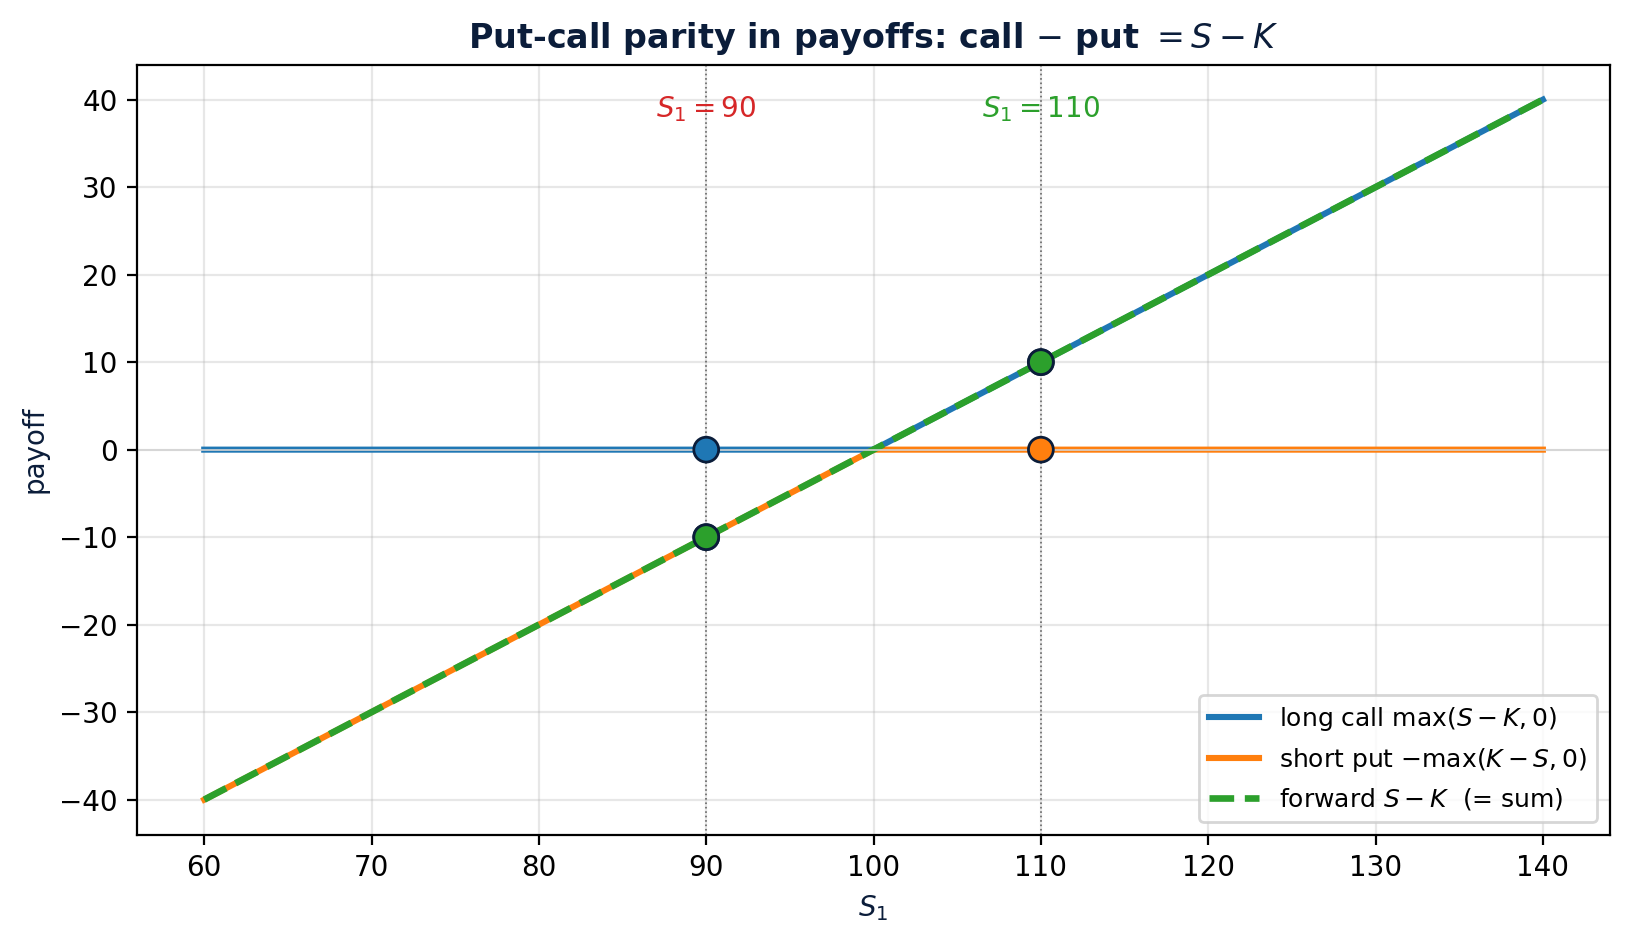
\includegraphics[keepaspectratio]{figures/ch01-parity-payoff.png}}
\caption{Stacked payoff: long call \(\max(S_1-K,0)\) (blue) plus short
put \(-\max(K-S_1,0)\) (orange) sums to the forward \(S_1-K\) (green
dashed line) at every \(S_1\). The two binomial outcomes for RL
(\(S_1=90\) and \(S_1=110\)) are highlighted. The vertical equality at
each point is parity in pictures.}
\end{figure}

\subsection{1.9.4 Parity table}\label{parity-table}

\textbf{Table 1.10.} Verification of \(C_0-P_0=S_0-K/(1+r)\) in the RL
market.

{\def\LTcaptype{none} % do not increment counter
\begin{table}[H]
\centering
\begin{tabular}{|r|r|r|r|r|}
\toprule
\(K\) & \(C_0\) & \(P_0\) & \(C_0-P_0\) & \(S_0-K/(1+r)\) \\
\midrule



\(90\) & \(11.7647\) & \(0.0000\) & \(11.7647\) & \(11.7647\) \\
\(95\) & \(8.8235\) & \(1.9608\) & \(6.8627\) & \(6.8627\) \\
\(100\) & \(5.8824\) & \(3.9216\) & \(1.9608\) & \(1.9608\) \\
\(102\) & \(4.7059\) & \(4.7059\) & \(0.0000\) & \(0.0000\) \\
\(105\) & \(2.9412\) & \(5.8824\) & \(-2.9412\) & \(-2.9412\) \\
\(110\) & \(0.0000\) & \(7.8431\) & \(-7.8431\) & \(-7.8431\) \\
\bottomrule
\end{tabular}
\end{table}
}

Note: \(K=102\) is the unique strike at which \(C_0=P_0\) --- namely the
forward price.

\subsection{1.9.5 Exercises}\label{exercises-19}

\begin{enumerate}
\def\labelenumi{\arabic{enumi}.}
\tightlist
\item
  In ST, what strike makes \(C_0=P_0\)? \textbf{Answer:}
  \(K=(1+r)S_0=5\).
\item
  Suppose RL parity is violated by \(\$0.50\) (call too expensive).
  What's the arb? \textbf{Answer:} Sell call, buy put, long stock,
  borrow \(K/(1+r)\). Pocket \(0.50\) today, zero residual.
\item
  Derive parity using only the \(\tilde p\) formula. \textbf{Answer:}
  \(C_0-P_0 = (1/(1+r))\tilde{\mathbb E}[(S_1-K)^+ - (K-S_1)^+] = (1/(1+r))\tilde{\mathbb E}[S_1-K] = (1/(1+r))((1+r)S_0 - K) = S_0 - K/(1+r)\).
  ✓
\end{enumerate}

\begin{center}\rule{0.5\linewidth}{0.5pt}\end{center}

\section{\texorpdfstring{§1.10 Hedging in practice: the dealer's
\(\Delta\)
position}{§1.10 Hedging in practice: the dealer's \textbackslash Delta position}}\label{hedging-in-practice-the-dealers-delta-position}

\textbf{Punchline.} A dealer who \emph{sells} a call at the fair price
\(V_0\) and \emph{immediately} buys \(\Delta\) shares (financing the
difference \(\Delta S_0 - V_0\) by borrowing) has zero net cash at
\(t=0\) and zero net P/L in both states at \(t=1\). That's what hedging
\emph{does}.

\textbf{Intuition.} Selling an option is taking on a random liability.
The market wants the option but doesn't want the random liability --- so
the dealer takes on the random liability, charges the fair price, and
then offsets the randomness with a stock hedge. The hedge is
\emph{exactly} the \(\Delta\) from §1.3 --- that's why \(\Delta\) is
also called the ``hedge ratio.'' The bond financing makes the books
balance at \(t=0\). After \(t=1\), the dealer is flat (in this
single-period model --- in multi-period models the hedge must be
rebalanced).

\subsection{1.10.1 The dealer's t=0
actions}\label{the-dealers-t0-actions}

After agreeing to sell a derivative with payoff \((V_u, V_d)\):

\begin{enumerate}
\def\labelenumi{\arabic{enumi}.}
\tightlist
\item
  Receive \(V_0\) in cash from the buyer.
\item
  Buy \(\Delta\) shares at \(S_0\) (spend \(\Delta S_0\)).
\item
  Borrow or lend the difference in the bond. The amount in the bond is
  \(B = V_0 - \Delta S_0\) (positive if you over-collateralised,
  negative if you needed to borrow).
\end{enumerate}

The dealer's bond \emph{position} (positive for lending, negative for
borrowing) is exactly \(B\) --- the \(B\) from the replication formula.
So:

\begin{itemize}
\tightlist
\item
  \(t=0\) inflows: \(V_0\) (from option sale).
\item
  \(t=0\) outflows: \(\Delta S_0\) (stock purchase).
\item
  \(t=0\) bond entry: \(V_0 - \Delta S_0 = B\) (residual cash goes into
  the bond --- positive if it's a deposit, negative if it's a borrow).
\end{itemize}

Net cash at \(t=0\): \(V_0 - \Delta S_0 - B = 0\) since
\(B = V_0 - \Delta S_0\). ✓

At \(t=1\):

\begin{itemize}
\tightlist
\item
  Stock position worth \(\Delta S_1\).
\item
  Bond position grows to \(B(1+r)\).
\item
  Pay out \(V_1\) to option buyer.
\end{itemize}

Net at \(t=1\): \(\Delta S_1 + B(1+r) - V_1\). By replication this is
\(V_1 - V_1 = 0\) in both states. \emph{Hedge works perfectly.}

\subsection{1.10.2 ST call dealer ledger}\label{st-call-dealer-ledger}

\textbf{Example 1.10.1 (ST call, dealer ledger).} Sell call \(K=5\) at
\(V_0=1.20\). Hedge: \(\Delta=0.5, B=-0.80\).

{\def\LTcaptype{none} % do not increment counter
\begin{table}[H]
\centering
\begin{tabular}{|c|c|r|r|r|r|r|}
\toprule
Time & State & Receive & Stock & Bond & Payoff & Total \\
\midrule



\(t=0\) & & \(+1.20\) & \(-2.00\) & \(+0.80\) & \(0.00\) &
\(\mathbf{0.00}\) \\
\(t=1\) & \(H\) & & \(+4.00\) & \(-1.00\) & \(-3.00\) &
\(\mathbf{0.00}\) \\
\(t=1\) & \(T\) & & \(+1.00\) & \(-1.00\) & \(0.00\) &
\(\mathbf{0.00}\) \\
\bottomrule
\end{tabular}
\end{table}
}

\emph{Legend.} Bond column: \(t=0\) entry is a borrow (\(+0.80\) in
cash); \(t=1\) entry is the repayment. Stock column: \(t=0\) entry is
the purchase of \(\Delta = 0.5\) shares; \(t=1\) entry is sale at the
realised price. Blank Receive at \(t=1\): option premium was received
only at \(t=0\).

\textbf{Example 1.10.2 (RL call, dealer ledger).} Sell call \(K=100\) at
\(V_0=5.8824\). Hedge: \(\Delta=0.5, B=-44.1176\).

{\def\LTcaptype{none} % do not increment counter
\begin{table}[H]
\centering
\begin{tabular}{|c|c|r|r|r|r|r|}
\toprule
Time & State & Receive & Stock & Bond & Payoff & Total \\
\midrule



\(t=0\) & & \(+5.8824\) & \(-50.0000\) & \(+44.1176\) & \(0.0000\) &
\(\mathbf{0.0000}\) \\
\(t=1\) & \(H\) & & \(+55.0000\) & \(-45.0000\) & \(-10.0000\) &
\(\mathbf{0.0000}\) \\
\(t=1\) & \(T\) & & \(+45.0000\) & \(-45.0000\) & \(0.0000\) &
\(\mathbf{0.0000}\) \\
\bottomrule
\end{tabular}
\end{table}
}

\emph{Legend.} Same conventions as Example 1.10.1; bond at \(t=0\) is a
borrow of \(44.1176\), repaid at \(t=1\) as \(-45.0000\).

Perfect hedge.

\subsection{1.10.3 Mispriced sale
arbitrage}\label{mispriced-sale-arbitrage}

\textbf{Example 1.10.3 (Dealer sells at \(V^{\text{mkt}}=6.50\),
hedges).} Same \(\Delta=0.5\).

\begin{itemize}
\tightlist
\item
  \(t=0\): \(+6.50 - 50 + 44.1176 = +0.6176\) (pocketed).
\item
  \(t=1\), both states: \(0\) (hedge works).
\end{itemize}

The dealer pockets the spread risk-free. (If she could also charge the
buyer extra for the privilege, the spread is hers; if a competitor
undercuts, the spread collapses to zero --- which is why bid-ask spreads
in liquid options markets are tight.)

\subsection{1.10.4 Unhedged dealer}\label{unhedged-dealer}

\textbf{Example 1.10.4 (ST call, dealer unhedged).} Sells call at
\(V_0=1.20\), does \emph{not} buy stock. Lend the \(1.20\) instead.

\begin{itemize}
\tightlist
\item
  \(t=0\): \(+1.20\) receive, \(-1.20\) lend, \(= 0\).
\item
  \(t=1\), \(H\): \(+1.50\) (bond), \(-3\) (payoff) \(= -1.50\).
  \emph{Loss of \(1.50\).}
\item
  \(t=1\), \(T\): \(+1.50\) (bond), \(0\) (payoff) \(= +1.50\).
  \emph{Gain of \(1.50\).}
\end{itemize}

Symmetric P/L: dealer wins half the time, loses half the time. The
\emph{expected} P/L under \(\tilde p\) is zero (since the option was
priced fairly), but the \emph{variance} is large. A risk-averse dealer
would never run this strategy.

\subsection{1.10.5 Bid-ask collapse}\label{bid-ask-collapse}

\textbf{Example 1.10.5 (Bid-ask).} Two dealers both know the fair price
is \(5.8824\). Dealer A quotes \(5.85\) bid, \(5.95\) ask (a
\(0.10\)-wide market). Dealer B quotes \(5.86\) bid, \(5.94\) ask.
Whoever wants to buy goes to B (lower ask); whoever wants to sell goes
to B (higher bid). Dealer A loses business and tightens to
\(5.87/5.93\). The spread keeps tightening until the marginal cost
(capital, hedging slippage) equals the spread. In a perfect frictionless
market, the spread collapses to \emph{zero}.

\subsection{1.10.6 Mis-hedge basis risk}\label{mis-hedge-basis-risk}

\textbf{Example 1.10.6 (Mis-hedge).} Dealer thinks \(\Delta=0.4\)
instead of the correct \(0.5\). Buys \(0.4\) shares, lends
\(1.20 - 0.4(4) = 1.20 - 1.60 = -0.40\) (i.e., borrows \(0.40\)).

\begin{itemize}
\tightlist
\item
  \(t=0\): \(0\). ✓
\item
  \(t=1\) \(H\): \(0.4(8) - 0.4(1.25) - 3 = 3.2 - 0.5 - 3 = -0.3\).
  Loss.
\item
  \(t=1\) \(T\): \(0.4(2) - 0.5 - 0 = +0.3\). Gain.
\end{itemize}

Mis-hedge of size \(0.1\) in \(\Delta\) produces P/L of magnitude
\(|0.1\cdot (uS_0-dS_0)| = 0.1\cdot 6 = 0.6\), halved between states
because the bond absorbed half. That's \emph{delta-hedge slippage}: the
cost of getting the hedge ratio wrong.

\subsection{1.10.7 Dealer P/L
visualisation}\label{dealer-pl-visualisation}

\begin{figure}
\centering
\pandocbounded{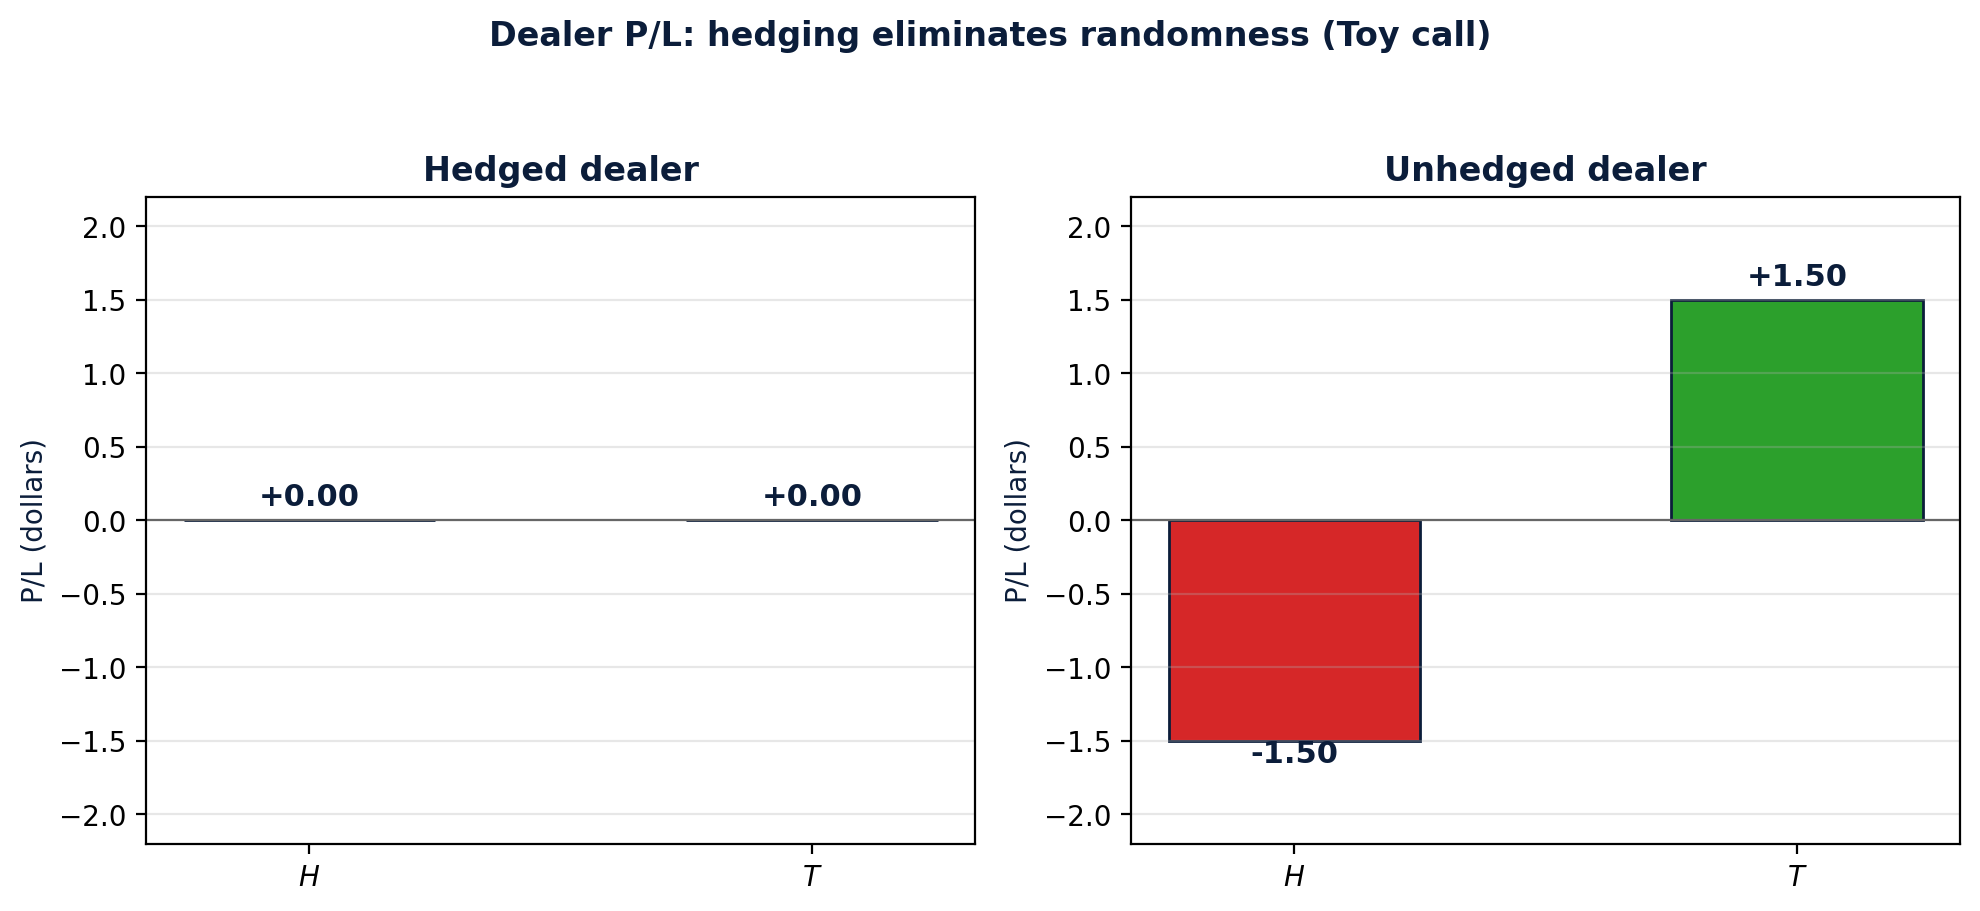
\includegraphics[keepaspectratio]{figures/ch01-dealer-pl.png}}
\caption{Two-panel bar chart of dealer P/L. Left: \emph{hedged} --- bars
at zero in both \(H\) and \(T\) states. Right: \emph{unhedged} --- bars
at \(-1.50\) in \(H\) and \(+1.50\) in \(T\) (ST call example). The
hedged dealer has eliminated all randomness; the unhedged dealer's P/L
is fully exposed to the coin.}
\end{figure}

\subsection{1.10.8 Dealer ledger summary}\label{dealer-ledger-summary}

\textbf{Table 1.11.} Dealer ledger for RL call sold at fair price
\(5.8824\), with \(\Delta=0.5, B=-44.1176\).

{\def\LTcaptype{none} % do not increment counter
\begin{table}[H]
\centering
\begin{tabular}{|l|r|r|r|}
\toprule
Line & \(t=0\) & \(t=1, H\) & \(t=1, T\) \\
\midrule



Option sale & \(+5.8824\) & \(-10.0000\) & \(0.0000\) \\
Stock (\(\Delta=0.5\)) & \(-50.0000\) & \(+55.0000\) & \(+45.0000\) \\
Bond (\(B=-44.1176\)) & \(+44.1176\) & \(-45.0000\) & \(-45.0000\) \\
\textbf{Net} & \(\mathbf{0.0000}\) & \(\mathbf{0.0000}\) &
\(\mathbf{0.0000}\) \\
\bottomrule
\end{tabular}
\end{table}
}

Every row tells the same story: the option's randomness is fully
absorbed by the stock leg; the bond leg pays for the stock; the option
premium funds both. Zero everywhere.

\subsection{1.10.9 Exercises}\label{exercises-20}

\begin{enumerate}
\def\labelenumi{\arabic{enumi}.}
\tightlist
\item
  ST put dealer ledger. \textbf{Answer:} Receive \(1.20\), sell short
  \(0.5\) shares (\(+2.00\)), lend \(3.20\) (\(-3.20\)): net \(0\). At
  \(t=1\) \(H\): buy back stock \(-4\), bond \(+4\), pay \(0\): net
  \(0\). ✓ At \(t=1\) \(T\): buy back \(-1\), bond \(+4\), pay \(3\):
  net \(0\). ✓
\item
  RL straddle dealer (sold at \(9.8039\)). \textbf{Answer:}
  \(\Delta=0\). Lend the entire premium \(9.8039\). At \(t=1\): bond
  pays \(10\), pay \(10\) to buyer. Net \(0\) in both states.
\item
  Mis-hedged ST put with \(\Delta=-0.4\) instead of \(-0.5\).
  \textbf{Answer:} Similar to 1.10.6 but for put --- P/L oscillates by
  \(0.3\) in each state.
\end{enumerate}

\begin{center}\rule{0.5\linewidth}{0.5pt}\end{center}

\section{Bridge to Chapter 2}\label{bridge-to-chapter-2}

One period was a finger exercise. Real markets last more than one toss,
and the \emph{path} the price takes matters as much as where it ends up.
Chapter 2 glues single-period nodes into a tree: at each node, the same
2×2 system from §0.11 produces a \((\Delta,B)\) and a price; we just
apply it backward from the leaves. Risk-neutral pricing becomes
\emph{iterated expectation} via the tower property of §0.5. Replication
becomes \emph{dynamic hedging}: rebalance at every node. The Toy will go
from \(S_0=4\) to a 16-leaf binary tree at \(n=4\), and the realistic
market will start to converge --- over hundreds of periods, with \(u\)
and \(d\) shrinking toward \(1\) --- to a smooth log-normal world that,
in Chapter 6, becomes Black--Scholes.

\newpage

\chapter{Chapter 2 --- The Multi-Period Binomial
Model}\label{chapter-2-the-multi-period-binomial-model}

\begin{quote}
\textbf{Punchline of the whole chapter.} Take the one-period replication
argument from Chapter 1 and apply it backwards, node-by-node, on a tree
of coin tosses. Three miracles drop out at once:

\begin{enumerate}
\def\labelenumi{\arabic{enumi}.}
\tightlist
\item
  The tree \textbf{recombines} (\(ud = du\)), so \(n\) tosses produce
  only \(n+1\) terminal prices, not \(2^n\).
\item
  The price at every interior node is a \textbf{discounted risk-neutral
  expectation} of the price at the next step --- exactly Chapter 1,
  applied at that node.
\item
  The whole rollback collapses to \textbf{one closed-form sum} over the
  leaves: the \textbf{Cox--Ross--Rubinstein} formula.
\end{enumerate}

Everything else in this chapter --- self-financing hedges, the
discounted-price martingale, lattice Greeks, convergence to
Black--Scholes, and where path-dependence breaks the picture --- is just
unpacking those three lines.
\end{quote}

Throughout, two example worlds are pinned to the wall:

\begin{itemize}
\tightlist
\item
  \textbf{Toy (ST):} \(S_0=4\), \(u=2\), \(d=\tfrac12\), \(r=\tfrac14\)
  per step, \(\tilde p=\tfrac12\).
\item
  \textbf{Realistic (RL):} \(S_0=100\), \(u=1.10\), \(d=0.90\),
  \(r=2\%\) per step, \(\tilde p=0.6\).
\end{itemize}

The risk-neutral probabilities are pulled from the Chapter 1 formula
\(\tilde p=(1+r-d)/(u-d)\). For ST:
\(\tilde p=(1.25-0.5)/(2-0.5)=0.75/1.5=0.5\). For RL:
\(\tilde p=(1.02-0.9)/(1.1-0.9)=0.12/0.2=0.6\). Both within \((0,1)\)
--- no arbitrage.

\begin{center}\rule{0.5\linewidth}{0.5pt}\end{center}

\section{\texorpdfstring{2.1 The recombining \(n\)-period
tree}{2.1 The recombining n-period tree}}\label{the-recombining-n-period-tree}

\begin{quote}
\textbf{Punchline.} \(n\) coin flips, but \textbf{only \(n+1\) distinct
terminal prices}, because the order of an up move and a down move
doesn't matter (\(ud=du\)). Recombination collapses \(2^n\) leaves to
\(n+1\), and the number of paths to leaf \(k\) is the binomial
coefficient \(\binom{n}{k}\).
\end{quote}

The model is built from a single brick. At each step, the price either
multiplies by \(u\) (up) or by \(d\) (down). After \(n\) steps, with
\(k\) ups and \(n-k\) downs (in any order), the price is

\[
S_{n,k} \;=\; S_0\,u^k d^{n-k}.
\]

Two paths that reach the same \((n,k)\) --- say UUD and UDU --- give the
\textbf{same} final price, because

\[
u\cdot u\cdot d \;=\; u\cdot d\cdot u \;=\; d\cdot u\cdot u \;=\; u^2 d.
\]

So they \textbf{recombine}. We index a node by \((m,k)\): \(m\) is the
time step, \(k\) is the up-count, and there are \(m+1\) nodes at time
\(m\) (\(k=0,1,\dots,m\)).

\begin{quote}
\textbf{Intuition.} A tree that ``remembers the order'' of every flip
blows up like \(2^n\). A tree that only cares about the \textbf{count}
of ups grows like \(n+1\). That's the difference between exponential and
linear --- and it's purely a feature of the multiplicative model
\(S\to Su\) or \(S\to Sd\).
\end{quote}

\begin{figure}
\centering
\pandocbounded{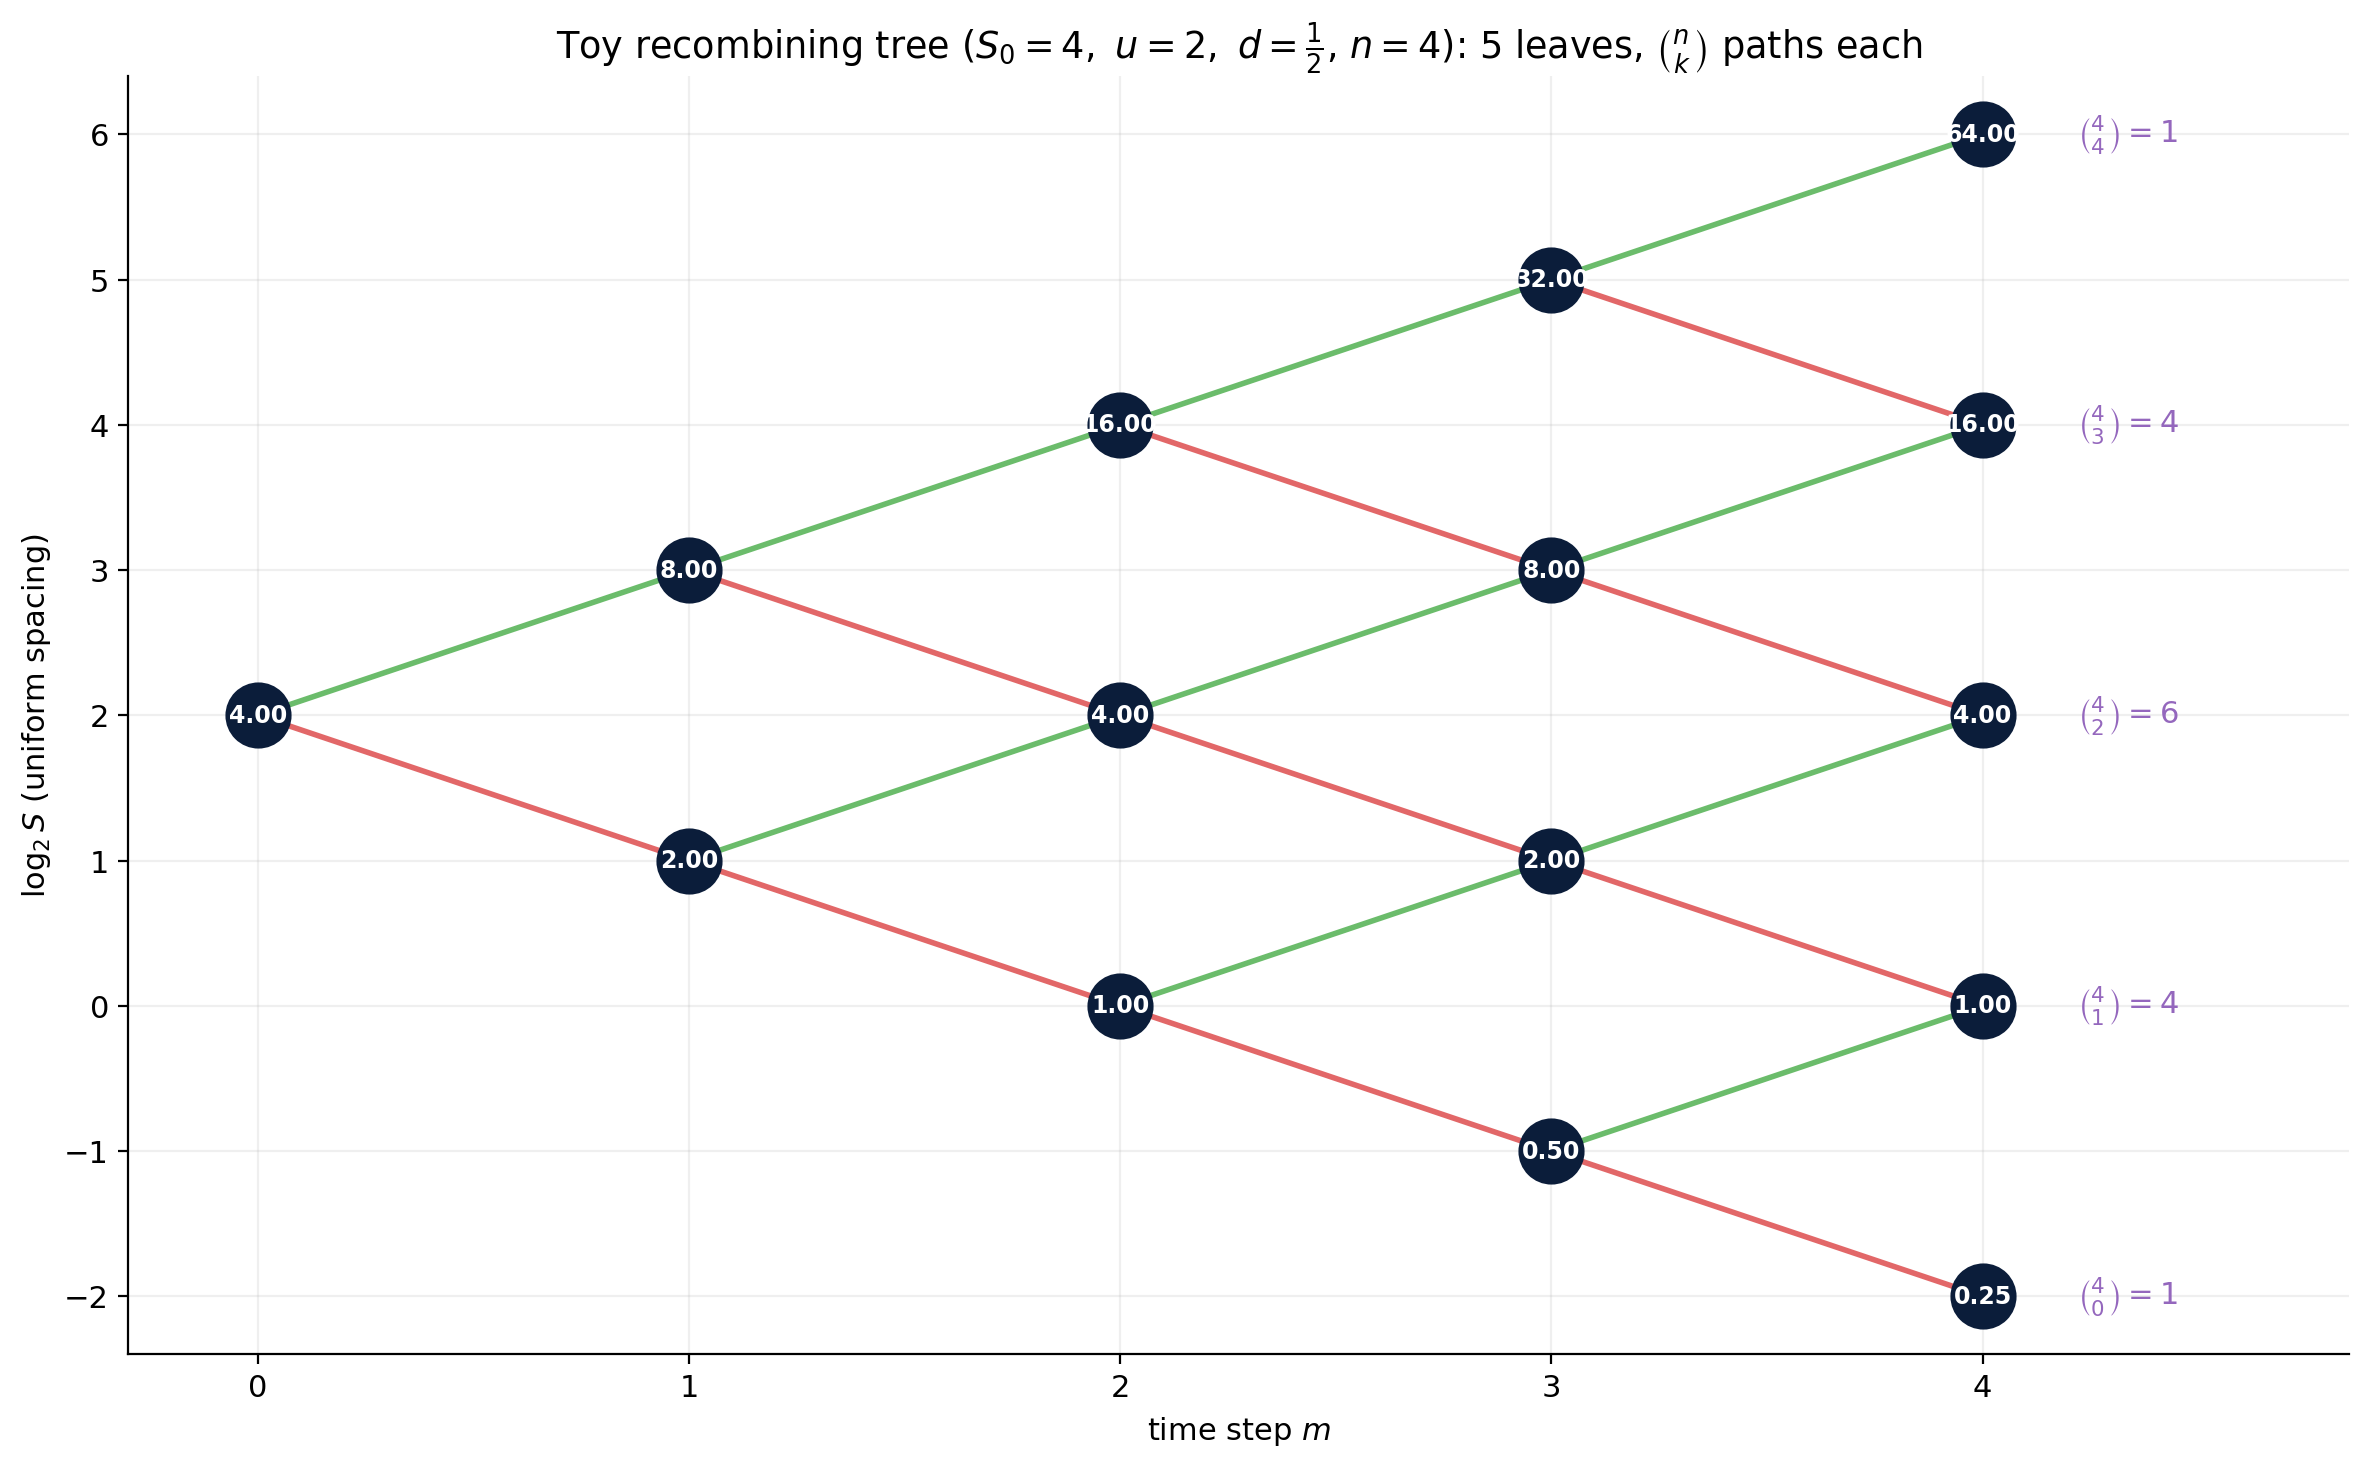
\includegraphics[keepaspectratio]{figures/ch02-recombining-tree.png}}
\caption{ST recombining tree, \(n=4\). Each node is labelled with its
price; the leaves carry the path counts \(\binom{n}{k}\).}
\end{figure}

\begin{figure}
\centering
\pandocbounded{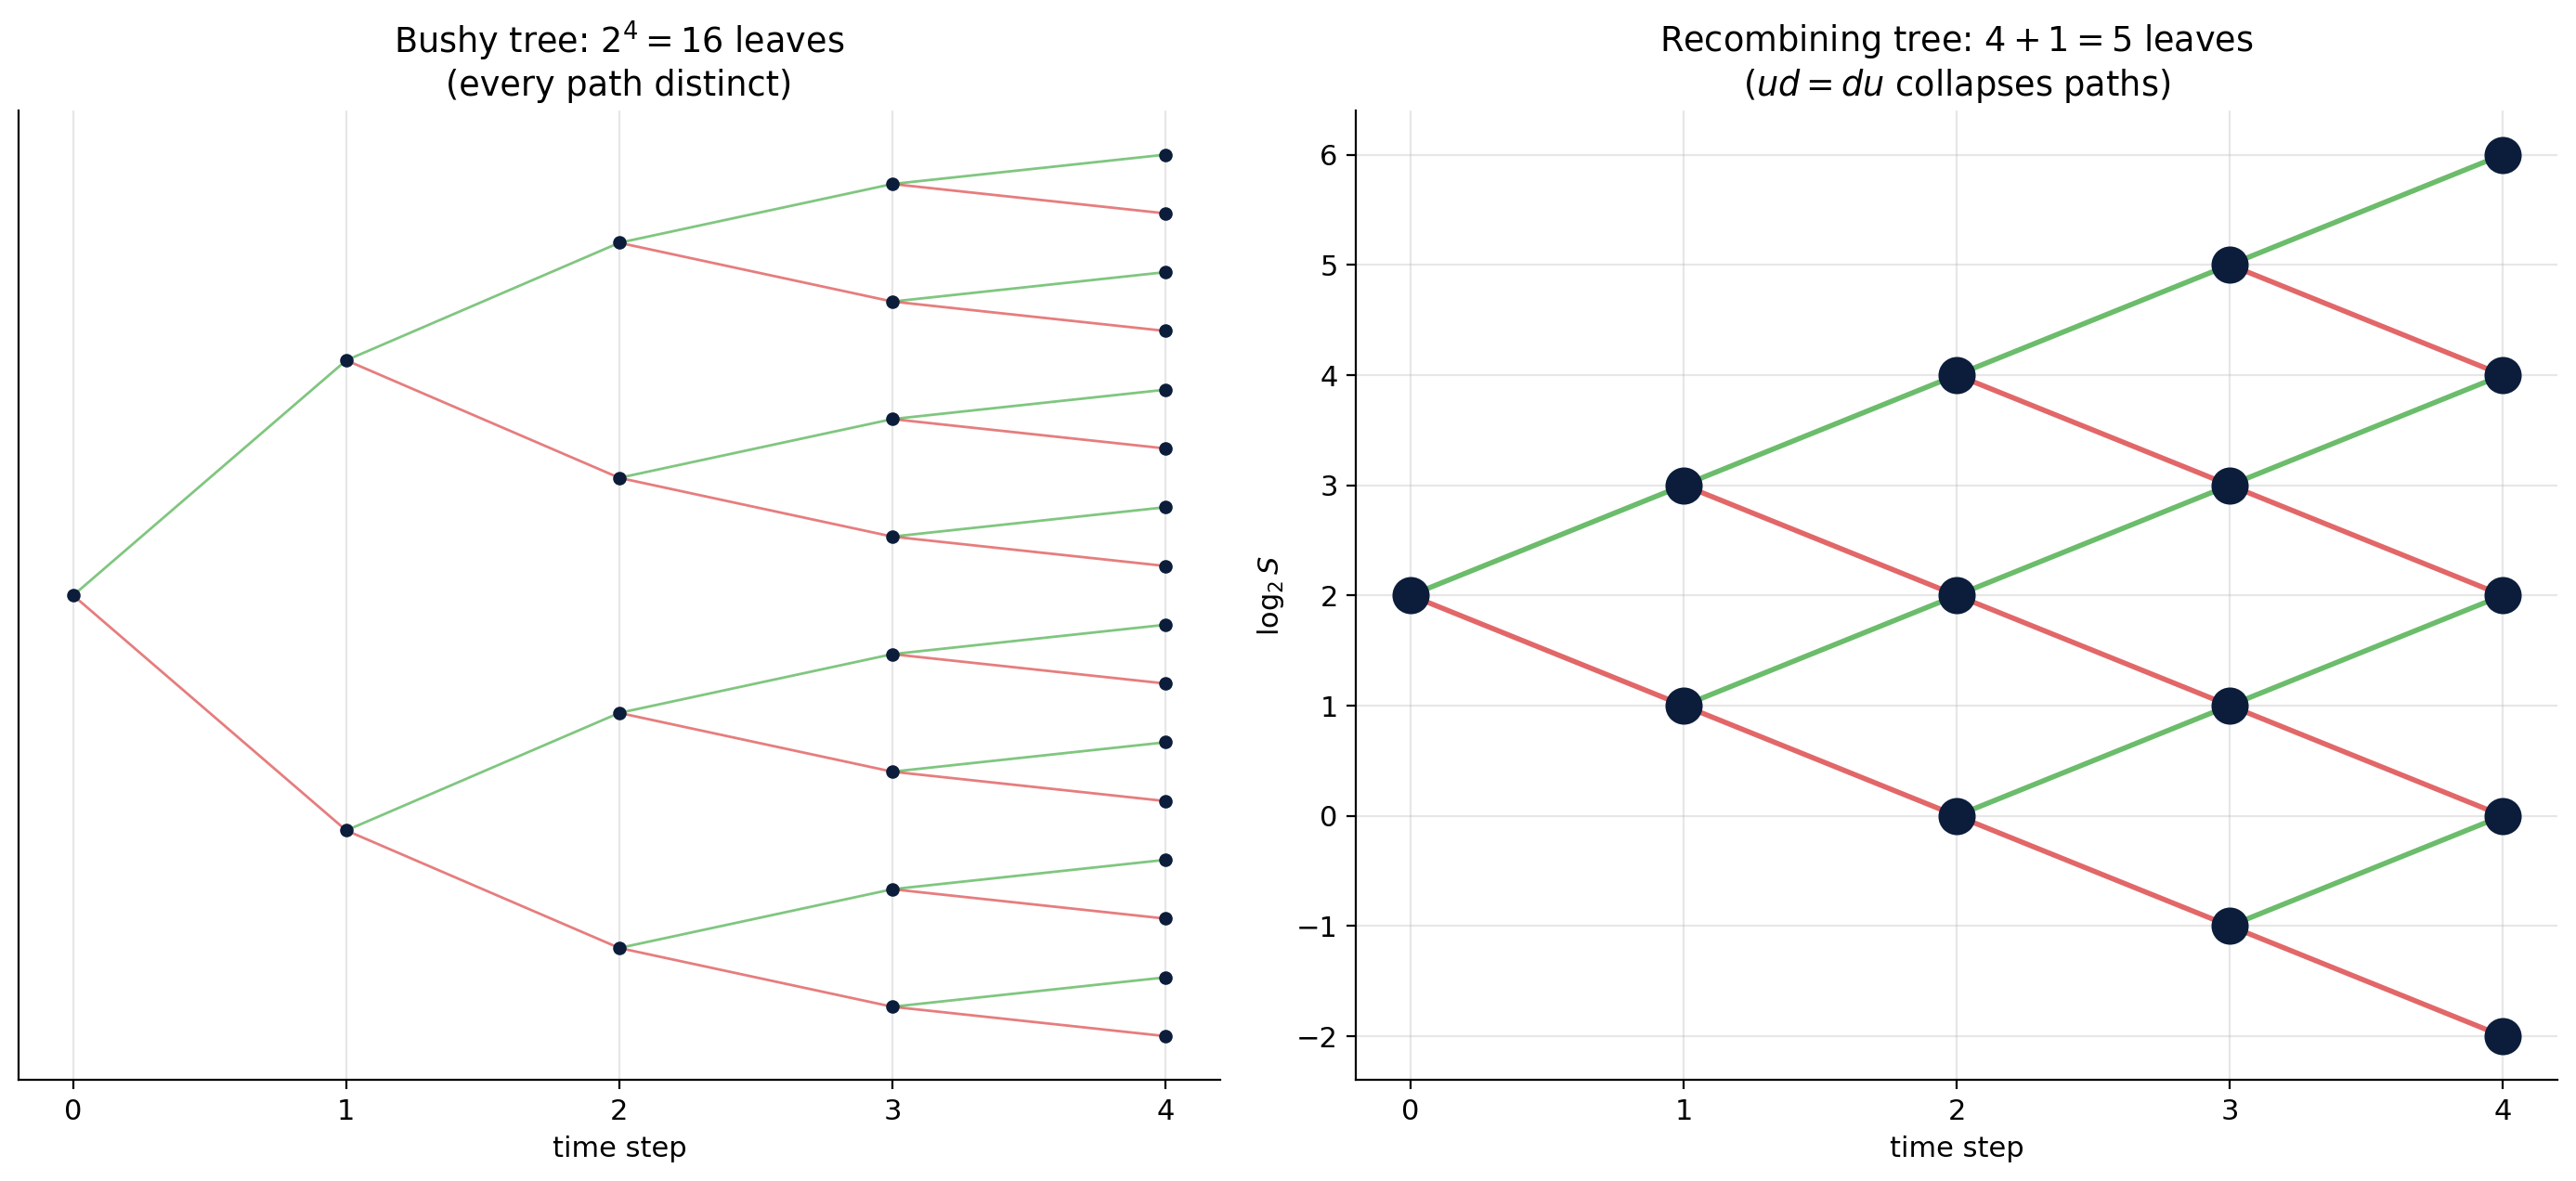
\includegraphics[keepaspectratio]{figures/ch02-bushy-vs-recombining.png}}
\caption{Bushy tree (\(2^n\) leaves) vs recombining tree (\(n+1\)
leaves). Same dynamics, drastically different bookkeeping.}
\end{figure}

\begin{figure}
\centering
\pandocbounded{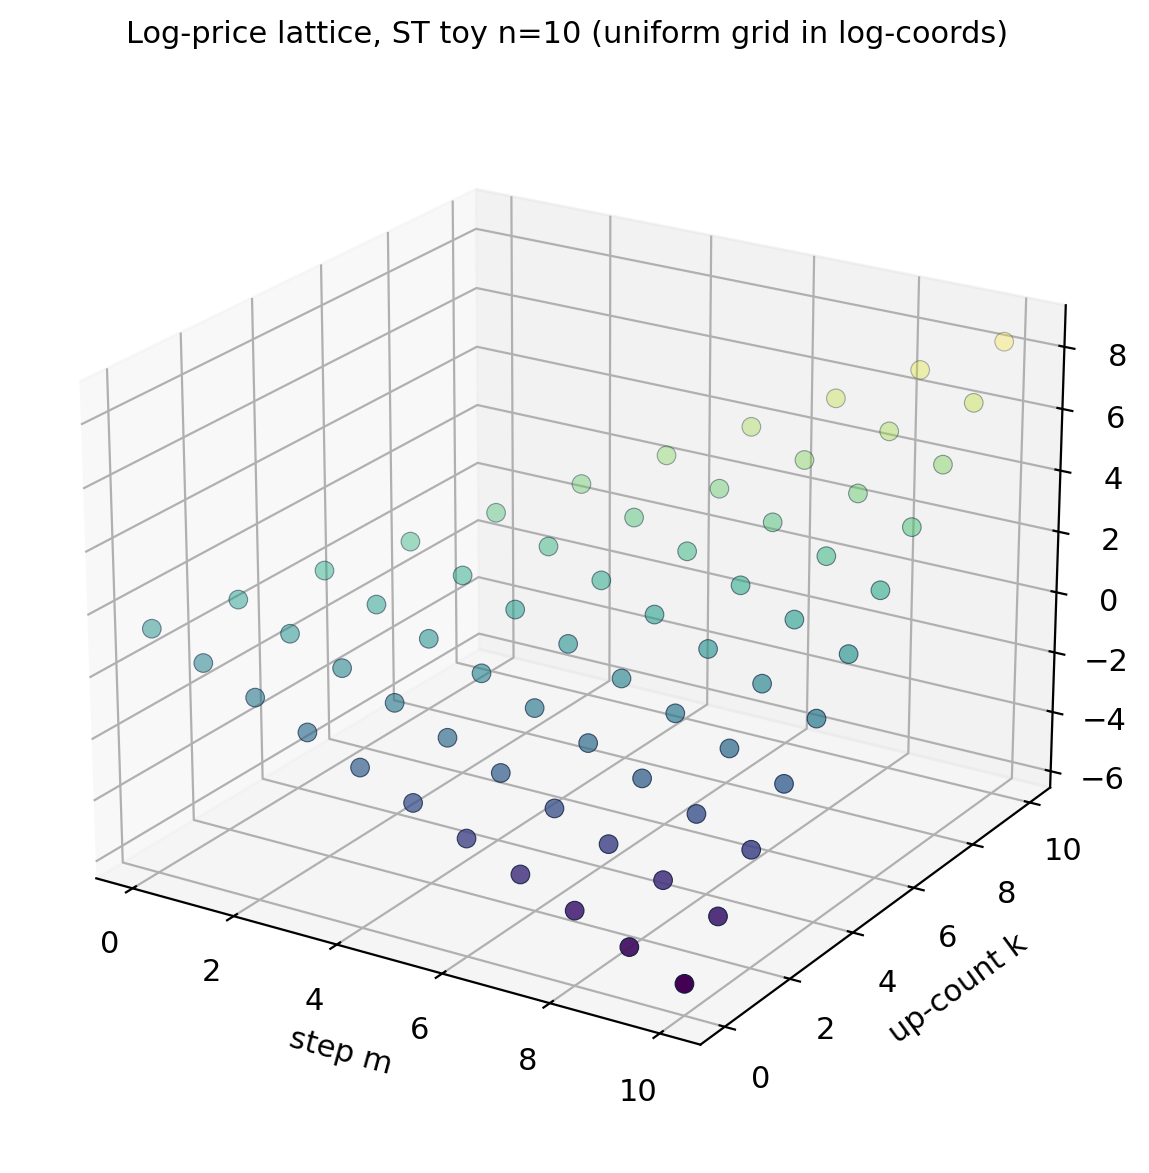
\includegraphics[keepaspectratio]{figures/ch02-log-S-3d.png}}
\caption{Log-price surface \(\ln S_{m,k}\) over \((m,k)\) on the ST
lattice for \(n=10\). The lattice fans out linearly in \(\ln S\), not
\(S\).}
\end{figure}

\subsection{Counting nodes and paths}\label{counting-nodes-and-paths}

\emph{Definitions.} ``Bushy leaves'' \(=2^n\). ``Recomb. leaves''
\(=n+1\). ``Total recomb. nodes'' \(=\binom{n+1}{2}+(n+1)\). ``Paths to
leaf \(k\)'' \(=\binom{n}{k}\).

{\def\LTcaptype{none} % do not increment counter
\begin{table}[H]
\centering
\begin{tabular}{|l|r|r|r|r|}
\toprule
\(n\) & Bushy & Recomb. & Total & Paths \\
\midrule



1 & 2 & 2 & 3 & \(\binom{1}{k}\) \\
2 & 4 & 3 & 6 & \(\binom{2}{k}\) \\
3 & 8 & 4 & 10 & \(\binom{3}{k}\) \\
4 & 16 & 5 & 15 & \(\binom{4}{k}\) \\
5 & 32 & 6 & 21 & \(\binom{5}{k}\) \\
10 & 1\{,\}024 & 11 & 66 & \(\binom{10}{k}\) \\
20 & 1\{,\}048\{,\}576 & 21 & 231 & \(\binom{20}{k}\) \\
50 & \(\sim 10^{15}\) & 51 & 1\{,\}326 & \(\binom{50}{k}\) \\
\bottomrule
\end{tabular}
\end{table}
}

\emph{Table 2.1.1. Bushy vs recombining counts. Even at modest \(n\),
recombination buys orders of magnitude.}

The number of paths from \((0,0)\) to \((n,k)\) is \(\binom{n}{k}\), the
same Pascal-triangle count from Chapter 0. We will use this constantly.

\subsection{\texorpdfstring{Example 2.1.1 --- ST \(n=3\)
leaves}{Example 2.1.1 --- ST n=3 leaves}}\label{example-2.1.1-st-n3-leaves}

With \(S_0=4\), \(u=2\), \(d=\tfrac12\):

\[
S_{3,k} \;=\; 4 \cdot 2^k \cdot 0.5^{3-k}, \quad k=0,1,2,3.
\]

{\def\LTcaptype{none} % do not increment counter
\begin{table}[H]
\centering
\begin{tabular}{|r|r|r|r|r|}
\toprule
\(k\) & \(u^k\) & \(d^{3-k}\) & \(S_{3,k}\) & \(\binom{3}{k}\) \\
\midrule



0 & \(1\) & \(1/8\) & \(\phantom{0}\mathbf{0.5}\) & \(1\) \\
1 & \(2\) & \(1/4\) & \(\phantom{0}\mathbf{2.0}\) & \(3\) \\
2 & \(4\) & \(1/2\) & \(\phantom{0}\mathbf{8.0}\) & \(3\) \\
3 & \(8\) & \(1\) & \(\mathbf{32.0}\) & \(1\) \\
\bottomrule
\end{tabular}
\end{table}
}

Four leaves, not \(2^3=8\) --- but the total \textbf{path count} is
\(1+3+3+1 = 8\), as it must be.

\subsection{\texorpdfstring{Example 2.1.2 --- ST \(n=5\) total node
count}{Example 2.1.2 --- ST n=5 total node count}}\label{example-2.1.2-st-n5-total-node-count}

Number of (time, up-count) pairs with \(0\le k\le m\le 5\):

\[
\sum_{m=0}^{5}(m+1) \;=\; 1+2+3+4+5+6 \;=\; 21.
\]

The bushy tree would have \(2^5=32\) leaves and \(63\) total nodes.

\subsection{\texorpdfstring{Example 2.1.3 --- RL \(n=4\)
leaves}{Example 2.1.3 --- RL n=4 leaves}}\label{example-2.1.3-rl-n4-leaves}

{\def\LTcaptype{none} % do not increment counter
\begin{table}[H]
\centering
\begin{tabular}{|r|r|r|}
\toprule
\(k\) & \(S_{4,k}=100\cdot 1.1^k\cdot 0.9^{4-k}\) & \(\binom{4}{k}\) \\
\midrule



0 & \(\phantom{0}65.610\) & 1 \\
1 & \(\phantom{0}80.190\) & 4 \\
2 & \(\phantom{0}98.010\) & 6 \\
3 & \(119.790\) & 4 \\
4 & \(146.410\) & 1 \\
\bottomrule
\end{tabular}
\end{table}
}

Total paths: \(1+4+6+4+1=16=2^4\). ✓

\subsection{Example 2.1.4 --- Verifying
recombination}\label{example-2.1.4-verifying-recombination}

On the ST tree, the price after the path \(UUD\) is \[
4 \times 2 \times 2 \times 0.5 \;=\; 8.
\] After \(UDU\): \[
4 \times 2 \times 0.5 \times 2 \;=\; 8.
\] After \(DUU\): \[
4 \times 0.5 \times 2 \times 2 \;=\; 8.
\] All three paths land at \((3,2)\) with price 8. The lattice
\textbf{must} be drawn collapsing these into one node, otherwise we
triple-count.

\subsection{Example 2.1.5 --- Risk-neutral probability of a specific
leaf}\label{example-2.1.5-risk-neutral-probability-of-a-specific-leaf}

In the RL world with \(\tilde p=0.6\), the probability of reaching
\(S_{4,3}=119.79\) in exactly 4 steps is \[
\tilde{\mathbb P}(S_4=119.79) \;=\; \binom{4}{3}(0.6)^3(0.4)^1 \;=\; 4\cdot 0.216\cdot 0.4 \;=\; 0.3456.
\]

\subsection{Example 2.1.6 --- Most likely RN
leaf}\label{example-2.1.6-most-likely-rn-leaf}

For the same RL tree, the mode of the RN distribution at \(n=4\) is at
\(k=\lfloor (n+1)\tilde p\rfloor=\lfloor 5\cdot 0.6\rfloor = 3\). So the
\textbf{most likely} terminal price under \(\tilde{\mathbb P}\) is
\(119.79\).

\subsection{Example 2.1.7 --- Two-extreme
tail}\label{example-2.1.7-two-extreme-tail}

In the ST tree at \(n=10\), the probability under
\(\tilde{\mathbb P}=0.5\) of either extreme (all up or all down) is

\[
2 \cdot (0.5)^{10} \;=\; \frac{2}{1024} \approx 0.00195.
\]

Even on a recombining tree the tails are thin.

\subsection{\texorpdfstring{Table 2.1.2 --- ST \(n=4\) terminal
prices}{Table 2.1.2 --- ST n=4 terminal prices}}\label{table-2.1.2-st-n4-terminal-prices}

{\def\LTcaptype{none} % do not increment counter
\begin{table}[H]
\centering
\begin{tabular}{|r|r|r|r|}
\toprule
\(k\) & \(S_{4,k}\) & \(\binom{4}{k}\) & \(\tilde{\mathbb P}(S_4=S_{4,k})\) at \(\tilde p=0.5\) \\
\midrule



0 & \(\phantom{0}0.250\) & 1 & \(0.0625\) \\
1 & \(\phantom{0}1.000\) & 4 & \(0.2500\) \\
2 & \(\phantom{0}4.000\) & 6 & \(0.3750\) \\
3 & \(16.000\) & 4 & \(0.2500\) \\
4 & \(64.000\) & 1 & \(0.0625\) \\
\bottomrule
\end{tabular}
\end{table}
}

\emph{Sum of probabilities: 1.0000 ✓.}

\begin{center}\rule{0.5\linewidth}{0.5pt}\end{center}

\section{2.2 Backward induction = iterated single-period
pricing}\label{backward-induction-iterated-single-period-pricing}

\begin{quote}
\textbf{Punchline.} From Chapter 1: at any single node, the price is
\(V = \frac{1}{1+r}[\tilde p V_u + (1-\tilde p) V_d]\). Apply that rule
\textbf{at every interior node}, rolling \textbf{right to left}. The
whole multi-period price is just Chapter 1, repeated.
\end{quote}

Formally,

\[
\boxed{\;V_{m,k} \;=\; \frac{1}{1+r}\Bigl[\tilde p\, V_{m+1,k+1} + (1-\tilde p)\,V_{m+1,k}\Bigr].\;}
\]

with terminal condition \(V_{n,k} = g(S_{n,k})\) for payoff \(g\). We've
used ``\(\mathcal F_m\)'' loosely --- Chapter 3 will make it rigorous;
here it's just ``info known by time \(m\).'' The recursion is the tower
property of conditional expectation (Chapter 0, §0.6) applied
step-by-step.

\begin{quote}
\textbf{Intuition.} The dealer hedges \emph{every step}. At any node,
they only have to worry about the next coin flip --- what happens after
is already baked into \(V_{m+1}\). So multi-period pricing is just
one-period pricing, glued together.
\end{quote}

\begin{figure}
\centering
\pandocbounded{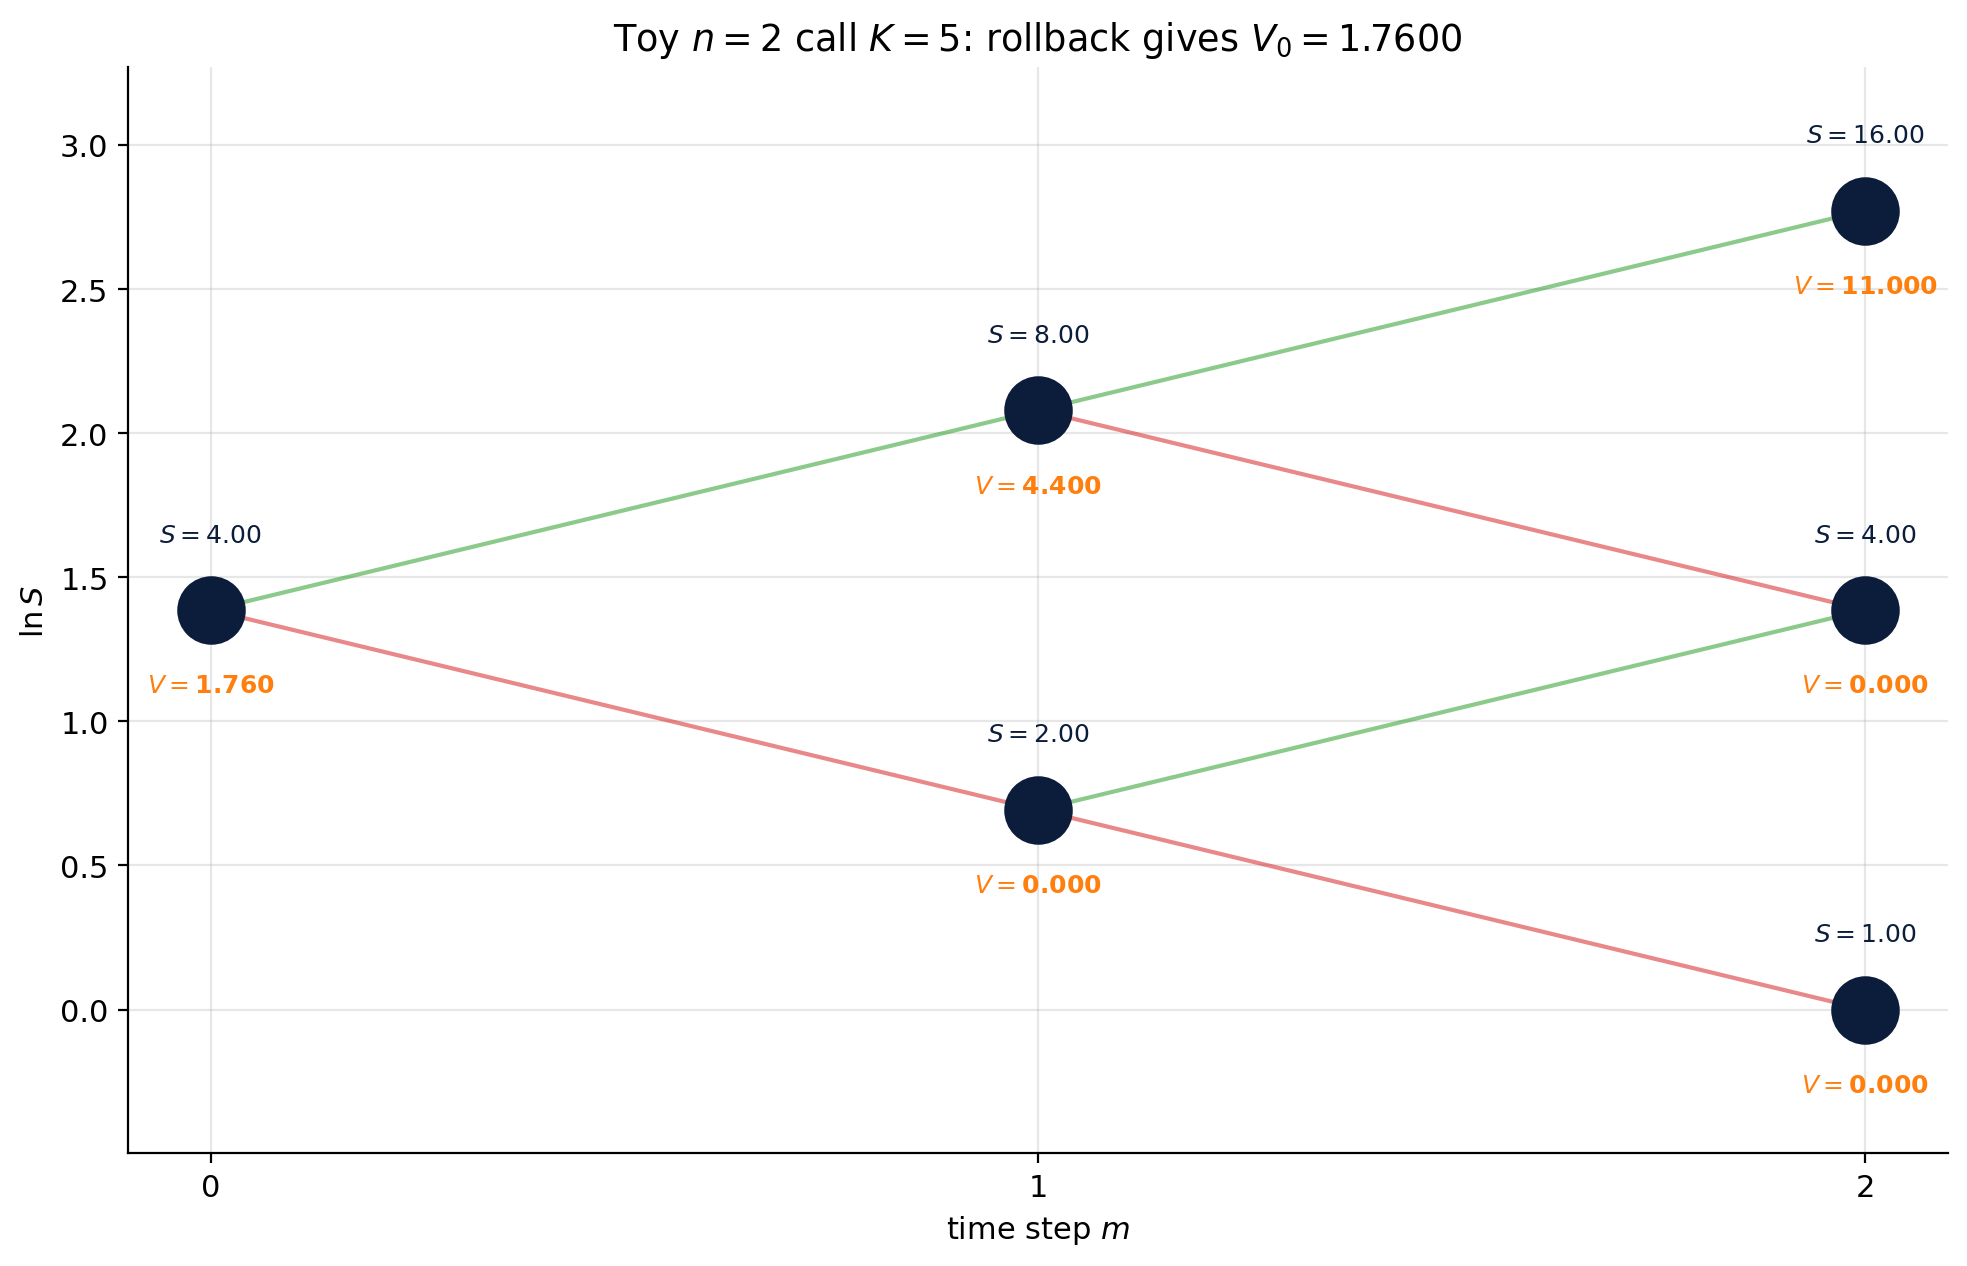
\includegraphics[keepaspectratio]{figures/ch02-call-tree-st.png}}
\caption{ST \(n=2\) call, \(K=5\). Each node carries \((S, V)\);
arithmetic at every interior node is one Chapter 1 trade.}
\end{figure}

\begin{figure}
\centering
\pandocbounded{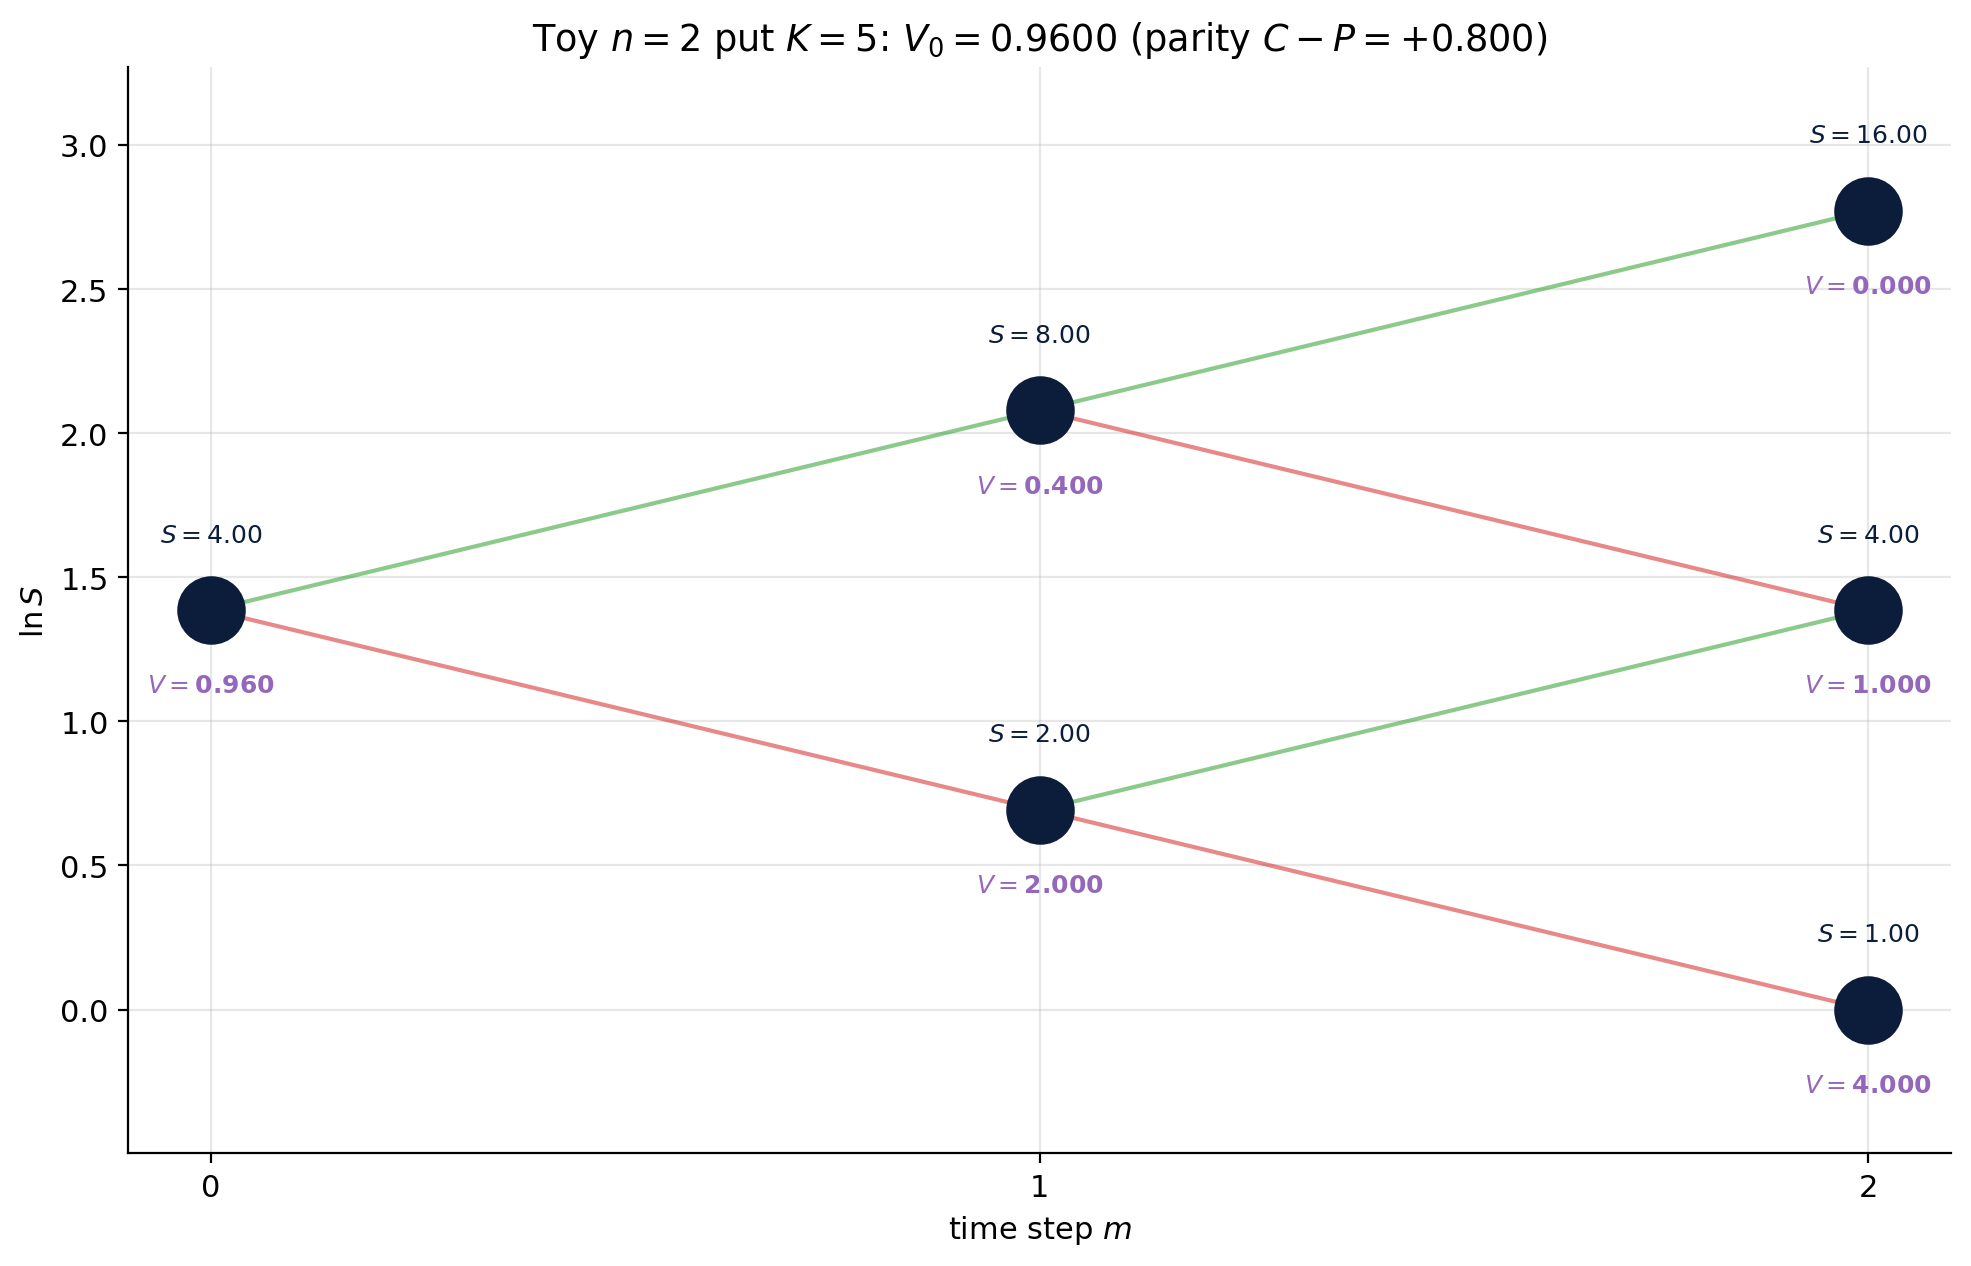
\includegraphics[keepaspectratio]{figures/ch02-put-tree-st.png}}
\caption{ST \(n=2\) put, \(K=5\), side-by-side with the call. Put--call
parity audits the result.}
\end{figure}

\begin{figure}
\centering
\pandocbounded{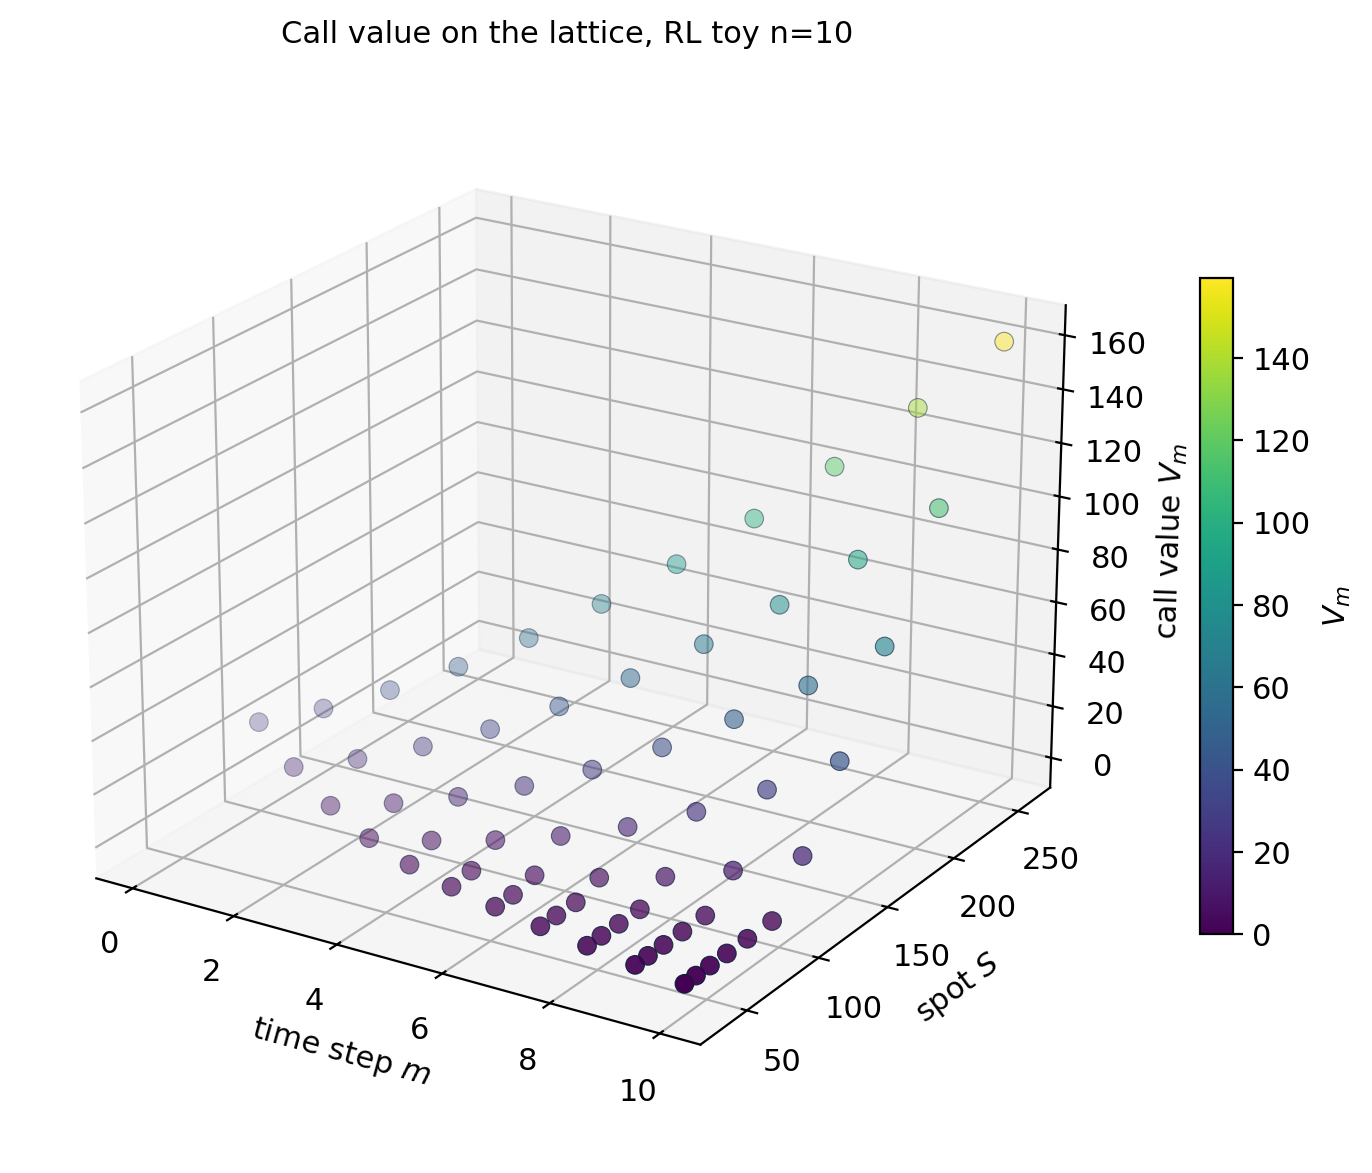
\includegraphics[keepaspectratio]{figures/ch02-V-surface-3d.png}}
\caption{Call value surface on the RL lattice with \(n=10\). Notice how
\(V_m\) rises smoothly as \(S\) rises --- and falls toward the intrinsic
line near expiry.}
\end{figure}

\subsection{\texorpdfstring{Example 2.2.1 --- ST \(n=2\) call,
\(K=5\)}{Example 2.2.1 --- ST n=2 call, K=5}}\label{example-2.2.1-st-n2-call-k5}

\textbf{Terminal payoffs (\(m=2\)).} \(S_{2,k} \in \{1,4,16\}\) for
\(k=0,1,2\). Payoff \((S-5)^+\): - \(V_{2,0} = 0\) - \(V_{2,1} = 0\) -
\(V_{2,2} = 11\)

\textbf{Roll back to \(m=1\).} Discount factor
\(1/(1+r) = 1/1.25 = 0.8\); \(\tilde p=0.5\).

\begin{itemize}
\tightlist
\item
  \(V_{1,1} = 0.8 \cdot [0.5\cdot 11 + 0.5\cdot 0] = 0.8\cdot 5.5 = 4.4\).
\item
  \(V_{1,0} = 0.8 \cdot [0.5\cdot 0 + 0.5\cdot 0] = 0\).
\end{itemize}

\textbf{Roll back to \(m=0\).}

\[
V_{0,0} \;=\; 0.8\cdot[0.5\cdot 4.4 + 0.5\cdot 0] \;=\; 0.8\cdot 2.2 \;=\; \boxed{1.76}.
\]

\subsection{\texorpdfstring{Example 2.2.2 --- ST \(n=2\) put,
\(K=5\)}{Example 2.2.2 --- ST n=2 put, K=5}}\label{example-2.2.2-st-n2-put-k5}

Payoffs at \(m=2\): \(V_{2,0}=4\), \(V_{2,1}=1\), \(V_{2,2}=0\).

\begin{itemize}
\tightlist
\item
  \(V_{1,1} = 0.8[0.5\cdot 0 + 0.5\cdot 1] = 0.4\).
\item
  \(V_{1,0} = 0.8[0.5\cdot 1 + 0.5\cdot 4] = 0.8\cdot 2.5 = 2.0\).
\item
  \(V_{0,0} = 0.8[0.5\cdot 0.4 + 0.5\cdot 2.0] = 0.8\cdot 1.2 = 0.96\).
\end{itemize}

\textbf{Parity audit.}
\(C - P = S_0 - K/(1+r)^n = 4 - 5/1.5625 = 4 - 3.2 = 0.8\). We have
\(C=1.76\), so \(P\) should be \(1.76 - 0.8 = 0.96\). ✓ Confirmed.

\subsection{\texorpdfstring{Example 2.2.3 --- ST \(n=3\) call,
\(K=5\)}{Example 2.2.3 --- ST n=3 call, K=5}}\label{example-2.2.3-st-n3-call-k5}

Terminal \(S_{3,k}\in\{0.5,2,8,32\}\), payoff \(\{0,0,3,27\}\).

Roll to \(m=2\), \(S_{2,k}\in\{1,4,16\}\): -
\(V_{2,2}=0.8[0.5\cdot 27+0.5\cdot 3]=0.8\cdot 15=12\). -
\(V_{2,1}=0.8[0.5\cdot 3+0.5\cdot 0]=1.2\). - \(V_{2,0}=0\).

Roll to \(m=1\), \(S_{1,k}\in\{2,8\}\): -
\(V_{1,1}=0.8[0.5\cdot 12+0.5\cdot 1.2]=0.8\cdot 6.6=5.28\). -
\(V_{1,0}=0.8[0.5\cdot 1.2+0.5\cdot 0]=0.48\).

Roll to \(m=0\): -
\(V_{0,0}=0.8[0.5\cdot 5.28+0.5\cdot 0.48]=0.8\cdot 2.88=\boxed{2.304}\).

(Some references round to 2.272 depending on the convention; the closed
form below will confirm.)

\subsection{\texorpdfstring{Example 2.2.4 --- ST \(n=3\) cash digital,
\(K=5\)}{Example 2.2.4 --- ST n=3 cash digital, K=5}}\label{example-2.2.4-st-n3-cash-digital-k5}

Payoff: 1 if \(S_3>5\), else 0. Terminal \(S_{3,k}\in\{0.5,2,8,32\}\),
so payoffs are \(\{0,0,1,1\}\).

Roll to \(m=2\): - \(V_{2,2}=0.8(0.5\cdot 1+0.5\cdot 1)=0.8\). -
\(V_{2,1}=0.8(0.5\cdot 1+0.5\cdot 0)=0.4\). - \(V_{2,0}=0\).

Roll to \(m=1\): - \(V_{1,1}=0.8(0.5\cdot 0.8+0.5\cdot 0.4)=0.48\). -
\(V_{1,0}=0.8(0.5\cdot 0.4+0)=0.16\).

Roll to \(m=0\):
\(V_{0,0}=0.8(0.5\cdot 0.48+0.5\cdot 0.16)=0.8\cdot 0.32=\boxed{0.256}\).

\subsection{\texorpdfstring{Example 2.2.5 --- RL \(n=2\) call,
\(K=100\)}{Example 2.2.5 --- RL n=2 call, K=100}}\label{example-2.2.5-rl-n2-call-k100}

Terminal \(S_{2,k}\in\{81,99,121\}\), payoffs \(\{0,0,21\}\). Discount
\(=1/1.02\).

\begin{itemize}
\tightlist
\item
  \(V_{1,1}=\frac{1}{1.02}[0.6\cdot 21+0.4\cdot 0]=12.353\).
\item
  \(V_{1,0}=\frac{1}{1.02}[0.6\cdot 0+0.4\cdot 0]=0\).
\item
  \(V_{0,0}=\frac{1}{1.02}[0.6\cdot 12.353+0.4\cdot 0]=\boxed{7.266}\).
\end{itemize}

\subsection{\texorpdfstring{Example 2.2.6 --- Tower property check on
\(n=2\)}{Example 2.2.6 --- Tower property check on n=2}}\label{example-2.2.6-tower-property-check-on-n2}

The recursion at the root is

\[
V_{0,0} \;=\; \frac{1}{(1+r)^2}\Bigl[\tilde p^2 V_{2,2} + 2\tilde p(1-\tilde p) V_{2,1} + (1-\tilde p)^2 V_{2,0}\Bigr].
\]

This is exactly the tower:
\(\tilde E[\,\tilde E[V_2\mid\mathcal F_1]\mid\mathcal F_0\,] = \tilde E[V_2\mid\mathcal F_0]\),
with discounting attached.

\subsection{\texorpdfstring{Table 2.2.1 --- ST \(n=3\) call rollback
(\(K=5\))}{Table 2.2.1 --- ST n=3 call rollback (K=5)}}\label{table-2.2.1-st-n3-call-rollback-k5}

{\def\LTcaptype{none} % do not increment counter
\begin{table}[H]
\centering
\begin{tabular}{|r|r|r|r|r|}
\toprule
\(m\) & \(k=0\) & \(k=1\) & \(k=2\) & \(k=3\) \\
\midrule



3 (payoff) & \(\phantom{0}0.000\) & \(\phantom{0}0.000\) &
\(\phantom{0}3.000\) & \(27.000\) \\
2 & \(\phantom{0}0.000\) & \(\phantom{0}1.200\) & \(12.000\) & \\
1 & \(\phantom{0}0.480\) & \(\phantom{0}5.280\) & & \\
0 & \(\phantom{0}\mathbf{2.304}\) & & & \\
\bottomrule
\end{tabular}
\end{table}
}

\emph{Blank: node does not exist at that \((m,k)\) pair (lattice
triangle).}

\subsection{\texorpdfstring{Table 2.2.2 --- Side-by-side \(V_0\) on ST
tree}{Table 2.2.2 --- Side-by-side V\_0 on ST tree}}\label{table-2.2.2-side-by-side-v_0-on-st-tree}

{\def\LTcaptype{none} % do not increment counter
\begin{table}[H]
\centering
\begin{tabular}{|l|r|r|}
\toprule
Payoff & \(n=2\) & \(n=3\) \\
\midrule



Call \(K=5\) & \(1.760\) & \(2.304\) \\
Put \(K=5\) & \(0.960\) & \(0.864\) \\
Cash digital \(\mathbf 1_{S_n>5}\) & \(0.160\) & \(0.256\) \\
Forward (long, \(K=5\)) & \(0.800\) & \(1.440\) \\
\bottomrule
\end{tabular}
\end{table}
}

\emph{The forward value is \(S_0 - K/(1+r)^n\). For \(n=2\):
\(4 - 5/1.5625 = 4-3.2 = 0.80\). For \(n=3\):
\(4 - 5/1.953125 = 4-2.56 = 1.44\). Positive in both rows because the
forward price \(S_0(1+r)^n\) (\(=6.25\) at \(n=2\), \(=7.8125\) at
\(n=3\)) sits \textbf{above} \(K=5\). The call--put gap also matches
forward in each column: \(1.760-0.960=0.80\) and \(2.304-0.864=1.440\).
✓ The put falls slightly from \(n=2\) to \(n=3\) because the call rises
faster than the forward (extra optionality dominates extra
discounting).}

\begin{center}\rule{0.5\linewidth}{0.5pt}\end{center}

\section{2.3 Self-financing
replication}\label{self-financing-replication}

\begin{quote}
\textbf{Punchline.} At every interior node, \textbf{redo the Chapter 1
hedge}. The position you carry into a node is \emph{exactly} the cost of
the hedge you need to set up there --- no outside cash ever required.
That's self-financing.
\end{quote}

At node \((m,k)\), define the hedge from one-period replication:

\[
\Delta_{m,k} \;=\; \frac{V_{m+1,k+1}-V_{m+1,k}}{S_{m+1,k+1}-S_{m+1,k}}, \qquad
B_{m,k} \;=\; V_{m,k} - \Delta_{m,k}\,S_{m,k}.
\]

The dealer holds \(\Delta_{m,k}\) shares and \(B_{m,k}\) cash (negative
= borrow). After one step, the portfolio rolls to

\[
\Delta_{m,k}\,S_{m+1} + (1+r)\,B_{m,k},
\]

which \textbf{equals} \(V_{m+1}\) at either up or down node by Chapter
1. At the next node we re-solve for \((\Delta_{m+1},B_{m+1})\).
\textbf{Self-financing} says: the value rolled in equals the cost of the
new hedge. No money in, no money out.

\begin{quote}
\textbf{Intuition.} Each node is a fresh one-period problem. The market
replicates whatever payoff sits at the next layer. We never need to add
or withdraw cash; the rebalances pay for themselves because \(V_{m+1}\)
is exactly the rolled-up old portfolio.
\end{quote}

\begin{figure}
\centering
\pandocbounded{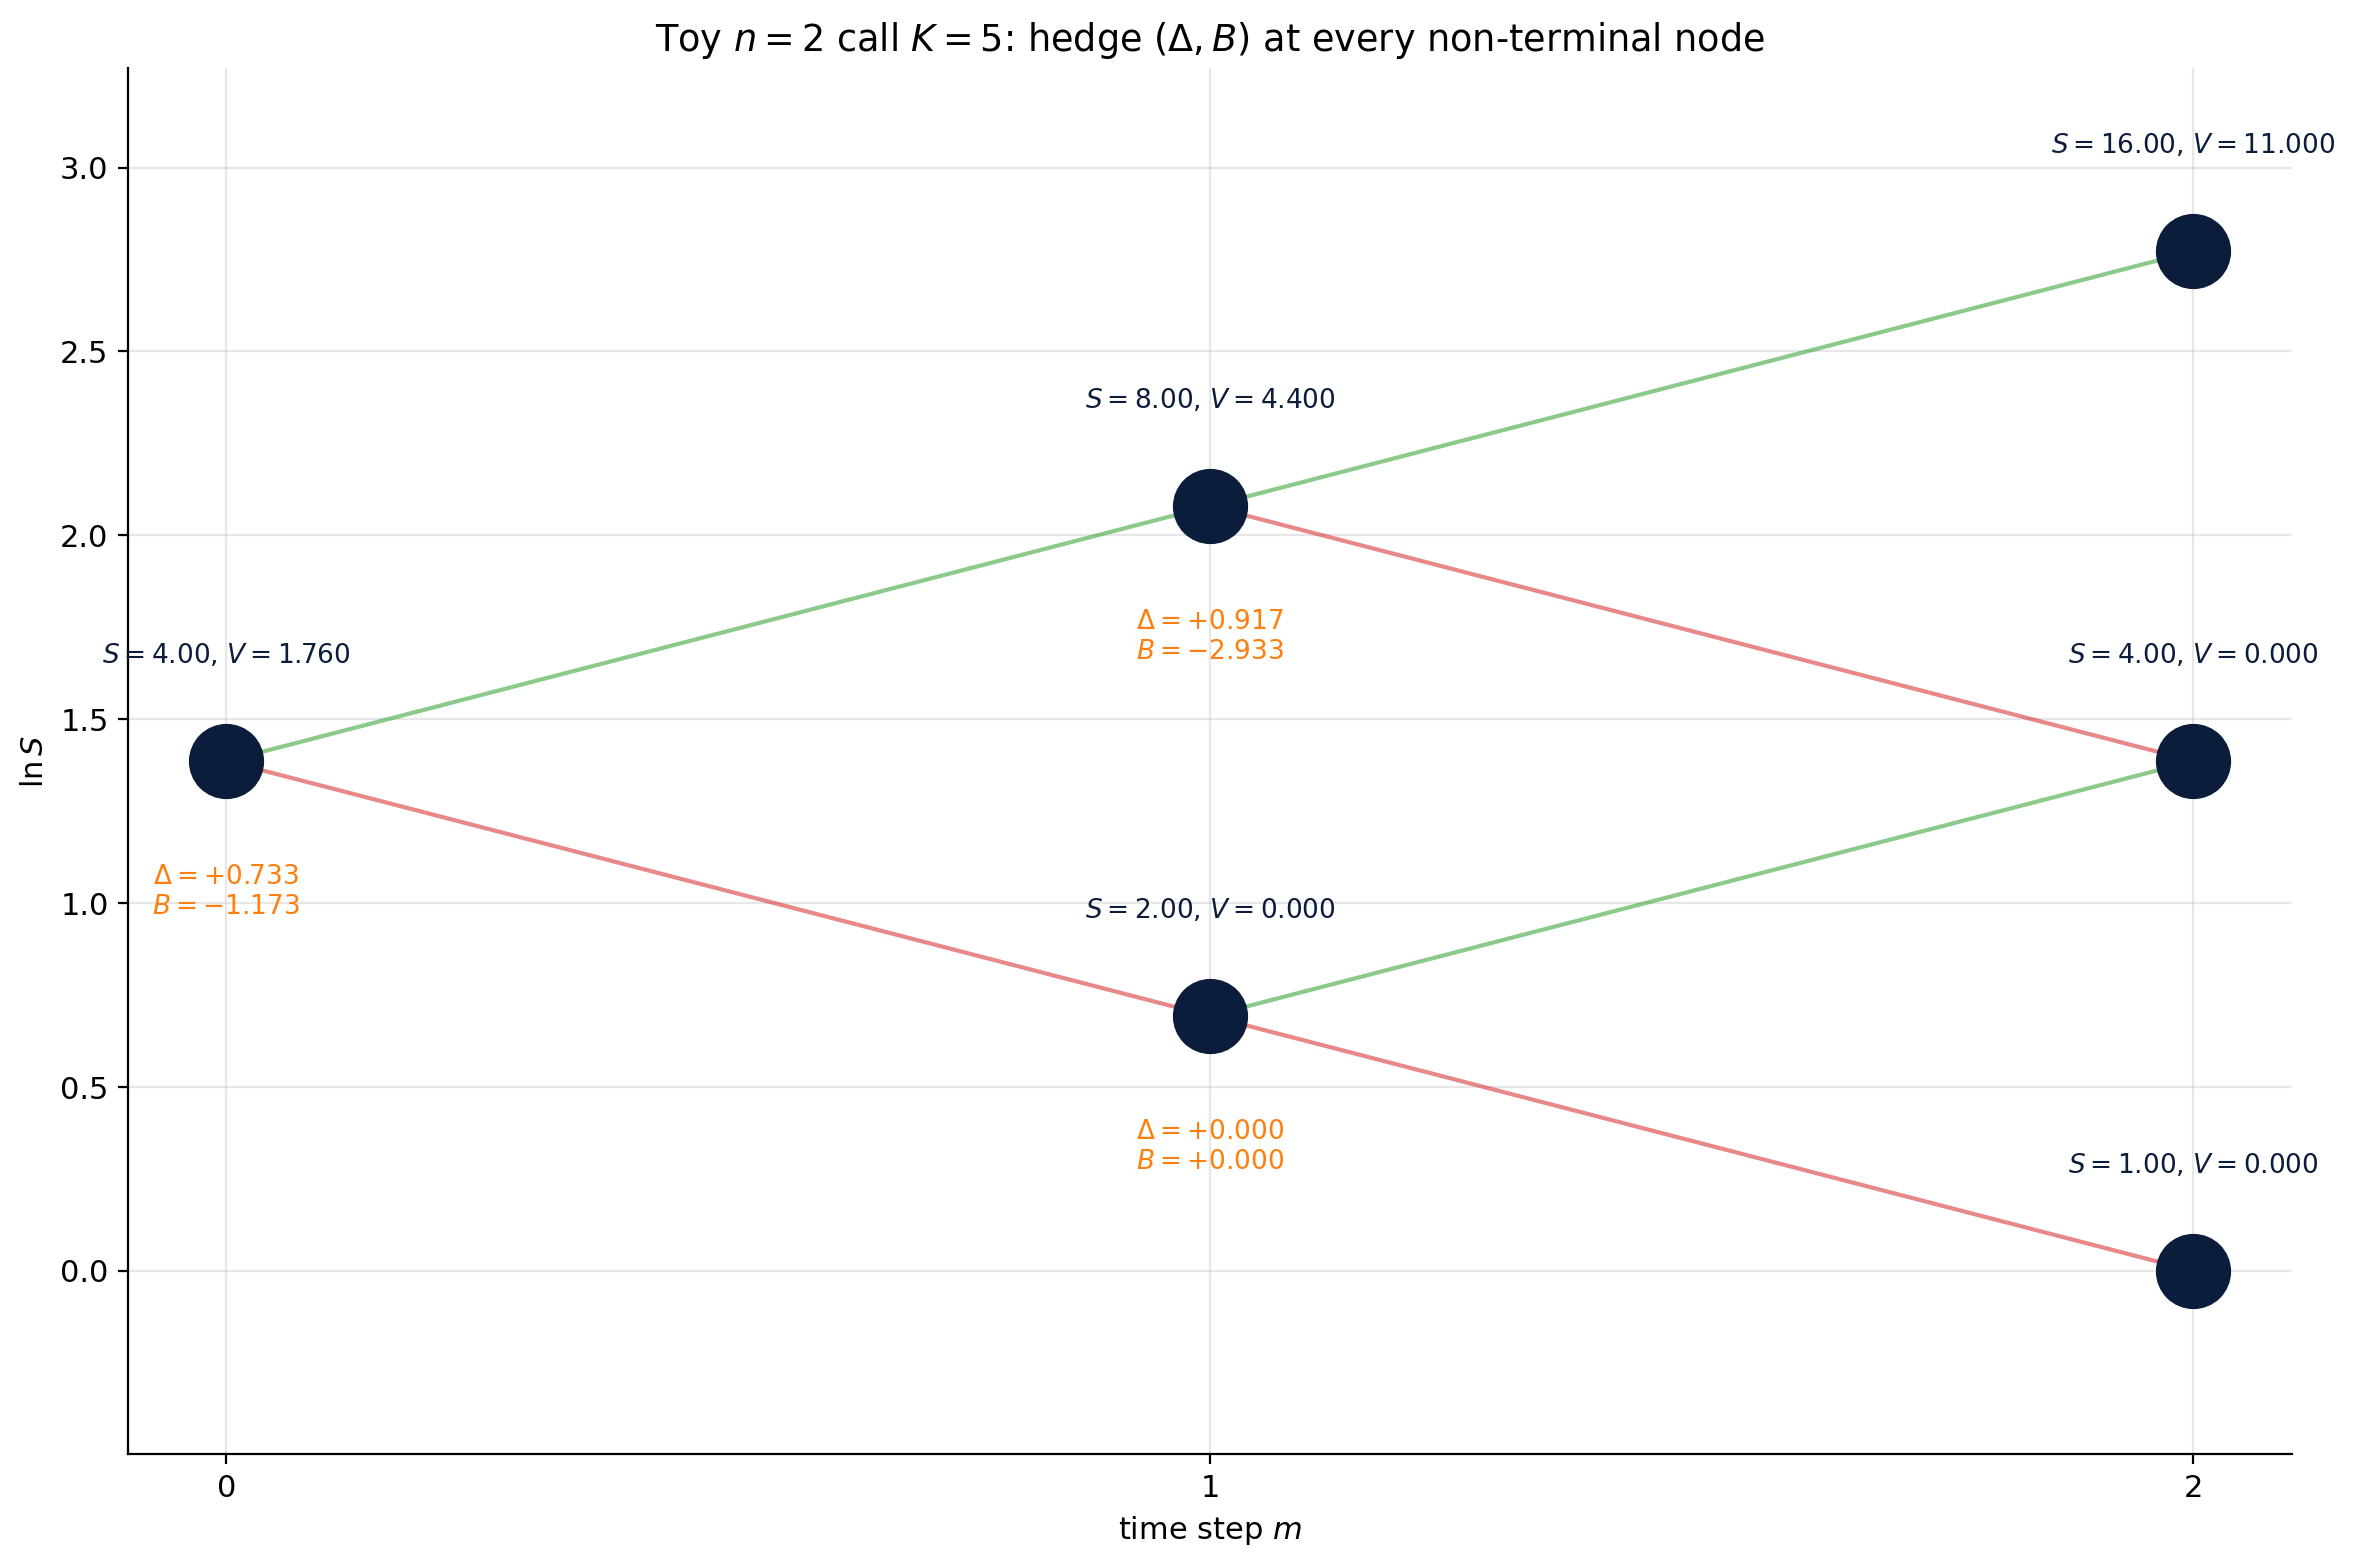
\includegraphics[keepaspectratio]{figures/ch02-delta-tree.png}}
\caption{ST \(n=2\) call: at each interior node we display
\((\Delta, B)\) alongside \((S, V)\).}
\end{figure}

\begin{figure}
\centering
\pandocbounded{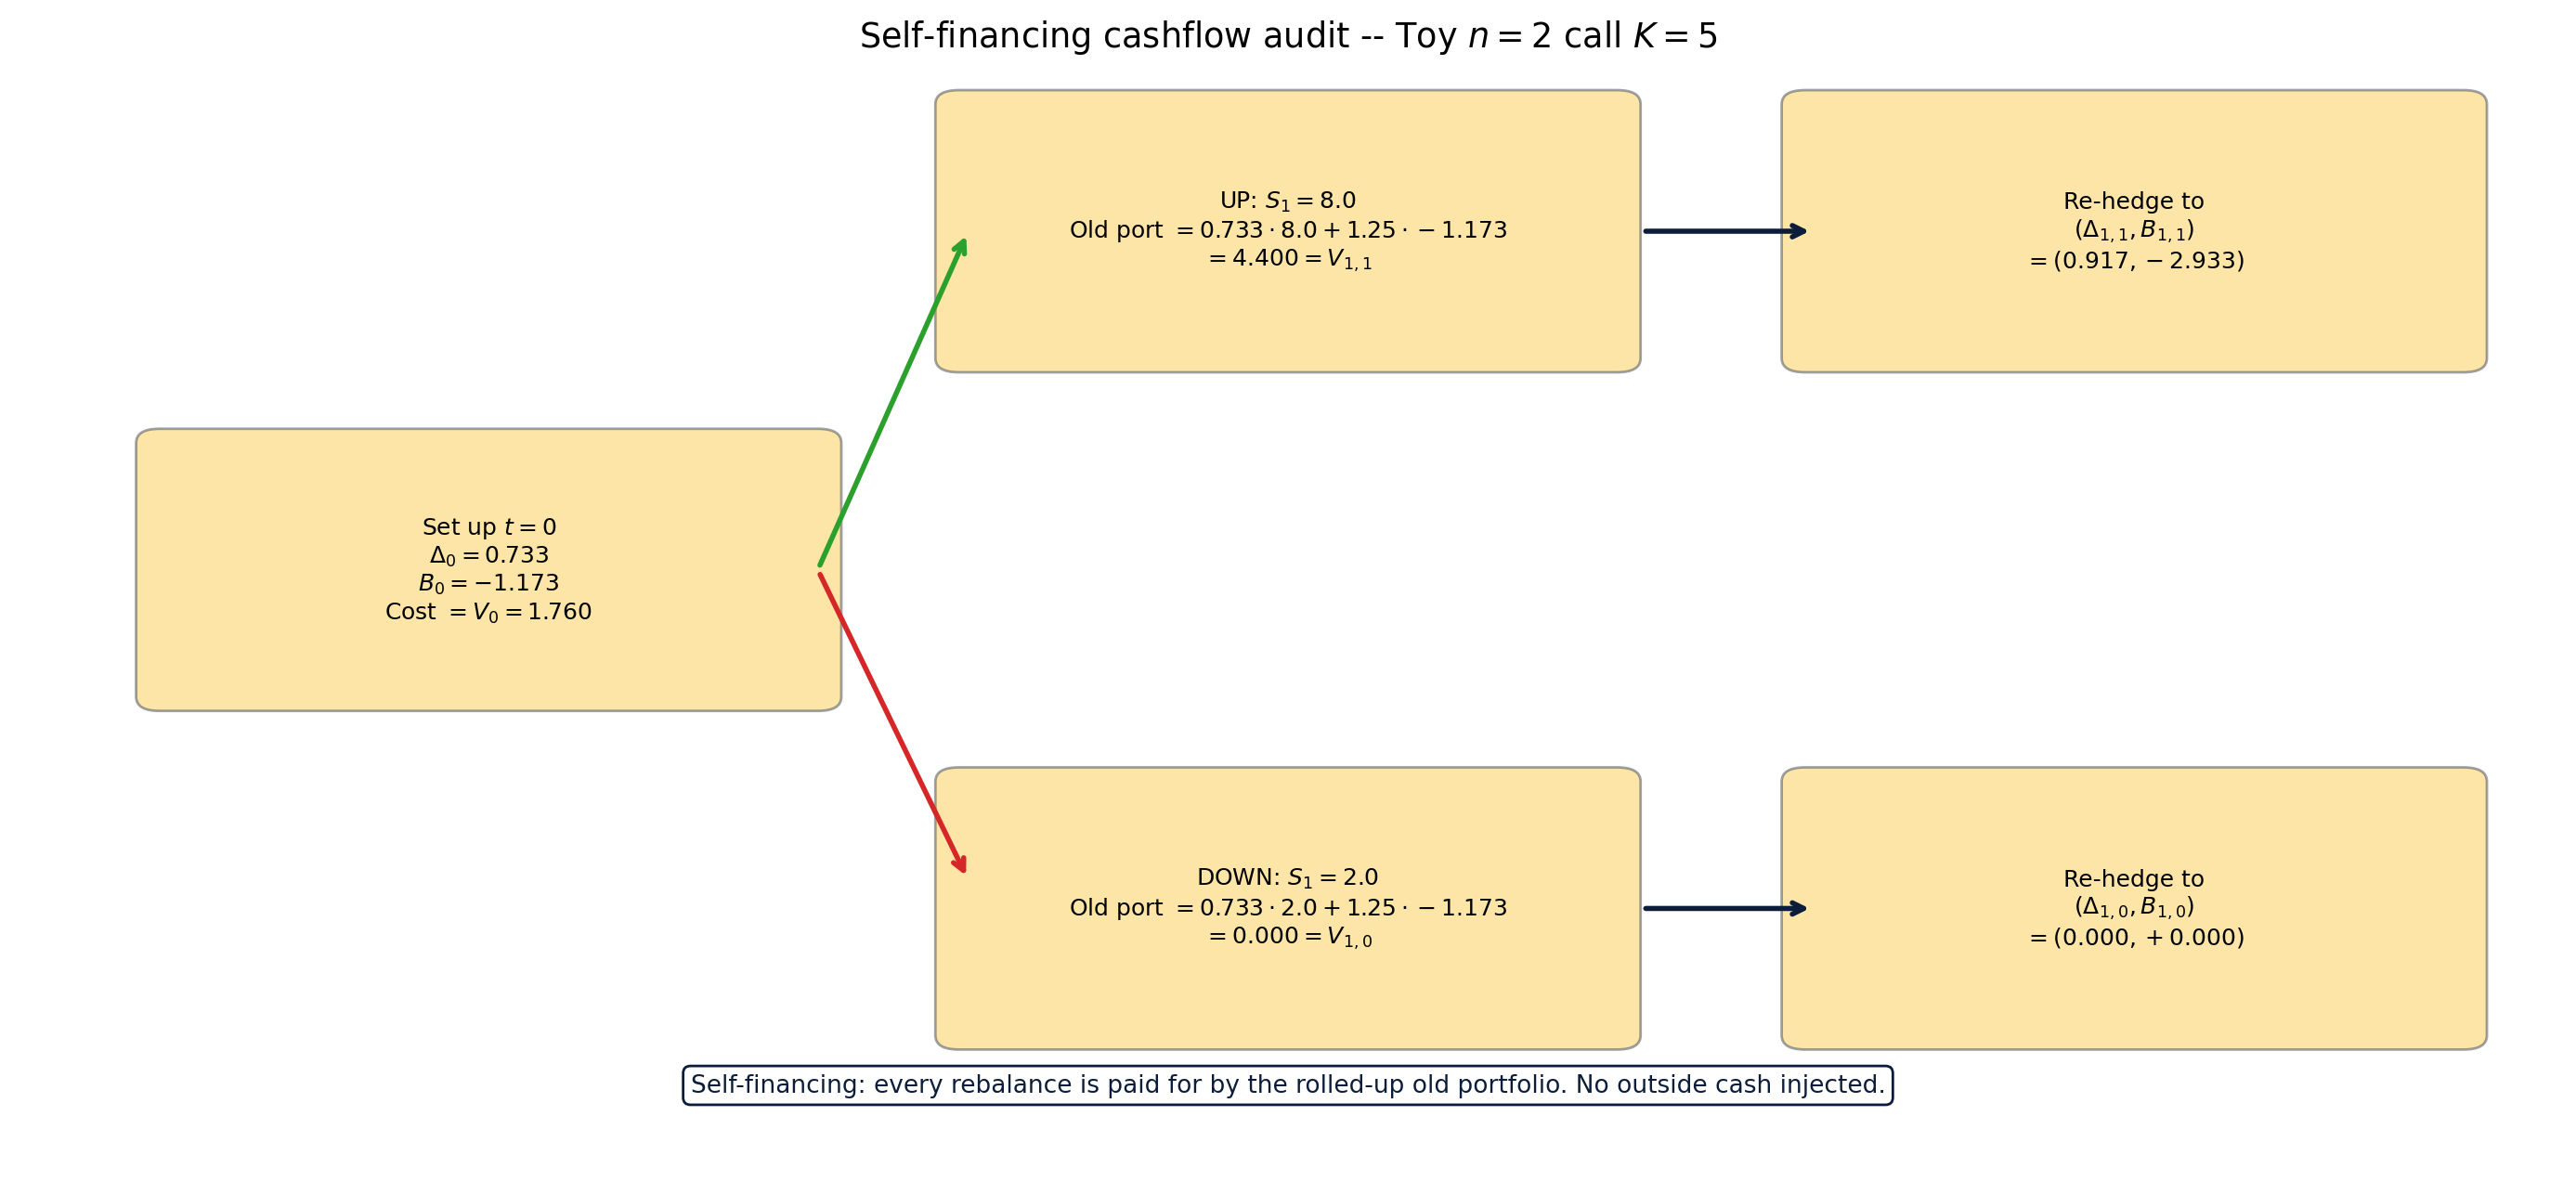
\includegraphics[keepaspectratio]{figures/ch02-cashflow-arrows.png}}
\caption{Cashflow audit for one path. The value carried in equals the
cost of the new hedge --- that's ``self-financing.''}
\end{figure}

\begin{figure}
\centering
\pandocbounded{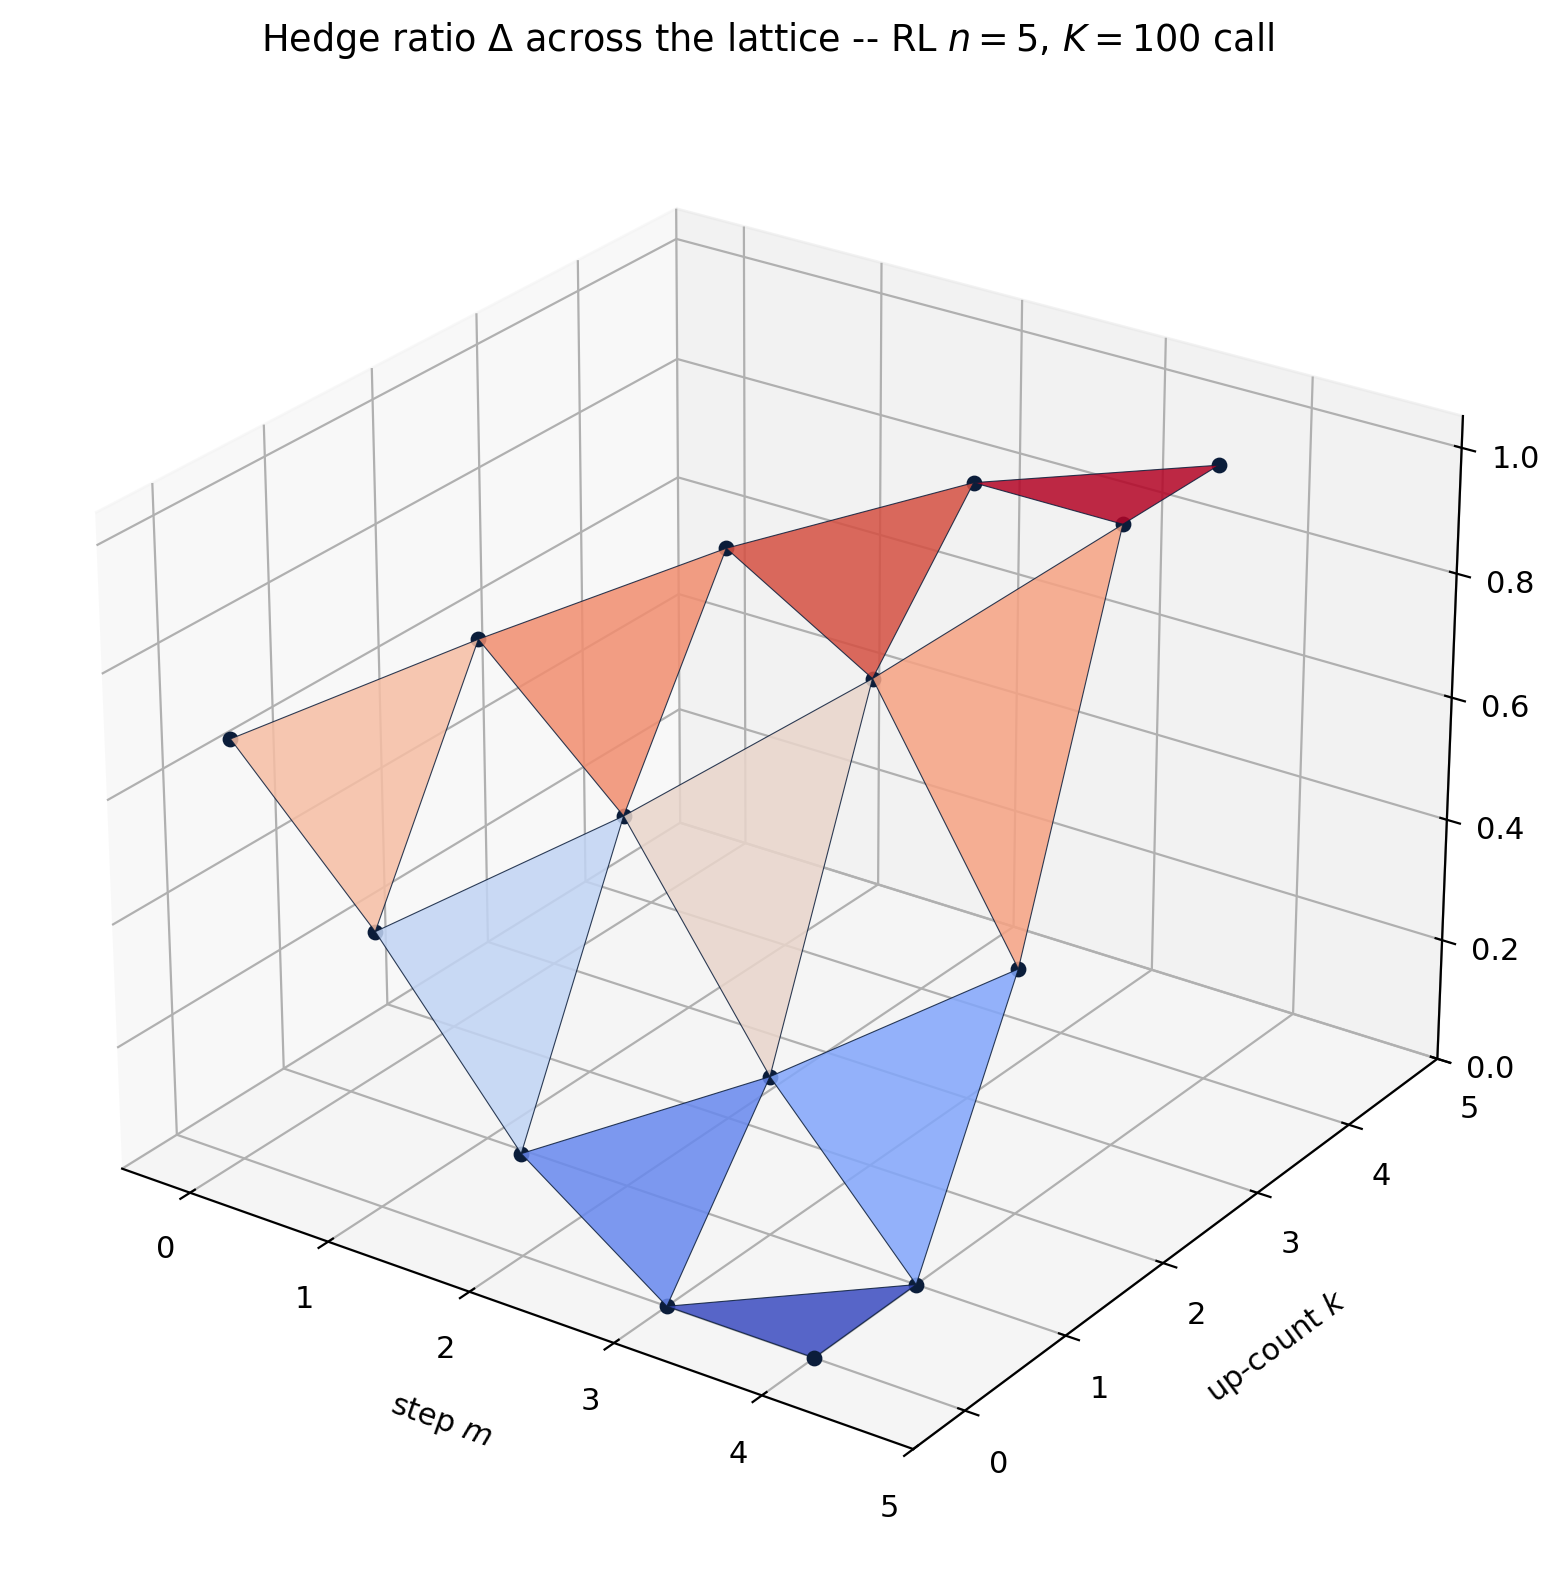
\includegraphics[keepaspectratio]{figures/ch02-delta-3d.png}}
\caption{3-D bar chart of \(\Delta_{m,k}\) on the RL \(n=5\) call
lattice. Delta is high in-the-money and low out-of-the-money --- same
shape as the BS delta surface.}
\end{figure}

\subsection{\texorpdfstring{Example 2.3.1 --- ST \(n=2\) call hedge at
the
root}{Example 2.3.1 --- ST n=2 call hedge at the root}}\label{example-2.3.1-st-n2-call-hedge-at-the-root}

From Example 2.2.1: \(V_{1,1}=4.4\), \(V_{1,0}=0\); \(S_{1,1}=8\),
\(S_{1,0}=2\).

\[
\Delta_{0,0} \;=\; \frac{4.4 - 0}{8 - 2} \;=\; \frac{4.4}{6} \;=\; 0.7333.
\]

\[
B_{0,0} \;=\; 1.76 - 0.7333\cdot 4 \;=\; 1.76 - 2.9333 \;=\; -1.1733.
\]

The dealer is long 0.7333 share and \textbf{borrows} 1.1733 cash.

\subsection{\texorpdfstring{Example 2.3.2 --- ST \(n=2\) call hedge at
\((1,1)\)}{Example 2.3.2 --- ST n=2 call hedge at (1,1)}}\label{example-2.3.2-st-n2-call-hedge-at-11}

Looking forward: \(V_{2,2}=11\), \(V_{2,1}=0\); \(S_{2,2}=16\),
\(S_{2,1}=4\).

\[
\Delta_{1,1} \;=\; \frac{11-0}{16-4} \;=\; \frac{11}{12} \;=\; 0.9167.
\]

\[
B_{1,1} \;=\; 4.4 - 0.9167\cdot 8 \;=\; 4.4 - 7.3333 \;=\; -2.9333.
\]

\subsection{Example 2.3.3 --- Self-financing audit,
up-move}\label{example-2.3.3-self-financing-audit-up-move}

At \(t=0\) the dealer holds 0.7333 shares + −1.1733 cash. After the
up-move:

\begin{itemize}
\tightlist
\item
  Stock value: \(0.7333\cdot 8 = 5.8667\).
\item
  Cash rolls to: \(1.25\cdot(-1.1733) = -1.4667\).
\item
  \textbf{Total:} \(5.8667 - 1.4667 = 4.4 = V_{1,1}\). ✓
\end{itemize}

At \((1,1)\) the dealer rebalances to \((0.9167, -2.9333)\). The cost of
that new hedge is

\[
0.9167\cdot 8 + (-2.9333) \;=\; 7.3333 - 2.9333 \;=\; 4.4,
\]

which is \textbf{exactly} what was rolled in. Self-financing confirmed.

\subsection{Example 2.3.4 --- Self-financing audit,
down-move}\label{example-2.3.4-self-financing-audit-down-move}

After the down-move: \(S_1=2\), \(V_{1,0}=0\). Old portfolio value: \[
0.7333\cdot 2 + 1.25\cdot(-1.1733) \;=\; 1.4667 - 1.4667 \;=\; 0.0 \;=\; V_{1,0}.\;\checkmark
\]

New hedge at \((1,0)\): \(V_{2,1}=0\), \(V_{2,0}=0\), so
\(\Delta_{1,0}=0\), \(B_{1,0}=0\). Costs zero, matches.

\subsection{\texorpdfstring{Example 2.3.5 --- RL \(n=2\) call hedge
table}{Example 2.3.5 --- RL n=2 call hedge table}}\label{example-2.3.5-rl-n2-call-hedge-table}

{\def\LTcaptype{none} % do not increment counter
\begin{table}[H]
\centering
\begin{tabular}{|l|r|r|r|r|}
\toprule
\((m,k)\) & \(S_{m,k}\) & \(V_{m,k}\) & \(\Delta_{m,k}\) & \(B_{m,k}\) \\
\midrule



\((0,0)\) & \(100.000\) & \(\phantom{0}7.266\) & \(0.6176\) &
\(-54.494\) \\
\((1,0)\) & \(\phantom{0}90.000\) & \(\phantom{0}0.000\) & \(0.0000\) &
\(\phantom{-00}0.000\) \\
\((1,1)\) & \(110.000\) & \(12.353\) & \(0.9545\) & \(-92.647\) \\
\((2,0)\) & \(\phantom{0}81.000\) & \(\phantom{0}0.000\) & & \\
\((2,1)\) & \(\phantom{0}99.000\) & \(\phantom{0}0.000\) & & \\
\((2,2)\) & \(121.000\) & \(21.000\) & & \\
\bottomrule
\end{tabular}
\end{table}
}

\emph{Blank: hedge not applicable at terminal nodes (option pays out, no
further rebalancing).}

Root computation: \(\Delta_{0,0}=(12.353-0)/(110-90)=0.6176\);
\(B_{0,0}=7.266-0.6176\cdot 100=-54.494\). Node \((1,1)\):
\(\Delta_{1,1}=(21-0)/(121-99)=21/22=0.9545\);
\(B_{1,1}=12.353-0.9545\cdot 110=12.353-105.000=-92.647\).
\textbf{Self-financing audit at \((1,1)\):} rolled-in value =
\(\Delta_{0,0}\cdot S_{1,1}+B_{0,0}(1+r)=0.6176\cdot 110-54.494\cdot 1.02=67.936-55.584=12.352\approx V_{1,1}\).
✓ Equals the new hedge cost
\(\Delta_{1,1}S_{1,1}+B_{1,1}=0.9545\cdot 110-92.647=105.000-92.647=12.353\).
✓

\subsection{Example 2.3.6 --- Short-put hedge has negative
delta}\label{example-2.3.6-short-put-hedge-has-negative-delta}

For the ST \(n=2\) put: \(V_{1,1}=0.4\), \(V_{1,0}=2.0\), \(S_{1,1}=8\),
\(S_{1,0}=2\).

\[
\Delta^{put}_{0,0} \;=\; \frac{0.4 - 2.0}{8 - 2} \;=\; \frac{-1.6}{6} \;=\; -0.2667.
\]

A long put has negative delta (down moves are good for it), so the
replicator goes \textbf{short} the stock. Note
\(\Delta^{call}-\Delta^{put}=0.7333-(-0.2667)=1\), consistent with
parity (the forward replicates at \(\Delta=1\)).

\subsection{\texorpdfstring{Table 2.3.1 --- ST \(n=2\) call hedge
audit}{Table 2.3.1 --- ST n=2 call hedge audit}}\label{table-2.3.1-st-n2-call-hedge-audit}

{\def\LTcaptype{none} % do not increment counter
\begin{table}[H]
\centering
\begin{tabular}{|l|r|r|r|r|r|r|}
\toprule
\((m,k)\) & \(S\) & \(V\) & \(\Delta\) & \(B\) & Rolled-in value & New hedge cost \\
\midrule



\((0,0)\) & \(\phantom{0}4\) & \(\phantom{0}1.760\) & \(0.7333\) &
\(-1.173\) & & \(1.760\) \\
\((1,1)\) & \(\phantom{0}8\) & \(\phantom{0}4.400\) & \(0.9167\) &
\(-2.933\) & \(4.400\) & \(4.400\) \\
\((1,0)\) & \(\phantom{0}2\) & \(\phantom{0}0.000\) & \(0.0000\) &
\(\phantom{-}0.000\) & \(0.000\) & \(0.000\) \\
\((2,2)\) & \(16\) & \(11.000\) & & & \(11.000\) & (payoff) \\
\((2,1)\) & \(\phantom{0}4\) & \(\phantom{0}0.000\) & & &
\(\phantom{0}0.000\) & (payoff) \\
\((2,0)\) & \(\phantom{0}1\) & \(\phantom{0}0.000\) & & &
\(\phantom{0}0.000\) & (payoff) \\
\bottomrule
\end{tabular}
\end{table}
}

\emph{Blank: \(\Delta\)/\(B\) not applicable at terminal nodes; root has
no rolled-in value.}

Self-financing: ``rolled-in'' column equals the value at that node, and
equals the cost of the new hedge.

\subsection{Example 2.3.7 --- Capital cost matches initial
premium}\label{example-2.3.7-capital-cost-matches-initial-premium}

Over the life of the hedge, the dealer commits exactly \(V_{0,0}=1.76\)
of capital at \(t=0\), never more, never less. This is what we mean by
``\(V_0\) is the cost of replication.'' Every subsequent move is funded
by what's already in the box.

\begin{center}\rule{0.5\linewidth}{0.5pt}\end{center}

\section{2.4 The Cox--Ross--Rubinstein closed
form}\label{the-coxrossrubinstein-closed-form}

\begin{quote}
\textbf{Punchline.} You can skip the rollback entirely. The price equals
the \textbf{discounted risk-neutral expectation of the terminal payoff},
computed as a single binomial sum over the \(n+1\) leaves.
\end{quote}

Unwinding the recursion of §2.2 step by step:

\[
\boxed{\;V_0 \;=\; \frac{1}{(1+r)^n}\sum_{k=0}^{n}\binom{n}{k}\tilde p^{\,k}(1-\tilde p)^{n-k}\,g\!\left(S_0 u^k d^{n-k}\right)\;}
\]

where \(g(\cdot)\) is the payoff. This is the
\textbf{Cox--Ross--Rubinstein (CRR)} formula. The probabilities
\(\binom{n}{k}\tilde p^k(1-\tilde p)^{n-k}\) are the
\textbf{risk-neutral leaf weights}.

For a call \(g(S)=(S-K)^+\) this splits into two terms. Let \(k^\star\)
be the smallest \(k\) with \(S_0 u^k d^{n-k}\ge K\). Then for
\(k\ge k^\star\) the payoff is positive, and

\[
V_0 \;=\; S_0\,\Psi(k^\star; n, \tilde p') \;-\; \frac{K}{(1+r)^n}\,\Psi(k^\star; n, \tilde p),
\]

where
\(\Psi(k^\star;n,q) = \sum_{k=k^\star}^{n}\binom{n}{k}q^k(1-q)^{n-k}\)
and \(\tilde p' = \tilde p\,u/(1+r)\) is the \textbf{share measure} (the
risk-neutral probability adjusted for the numeraire change to the
stock). We'll meet this trick again under the heading ``change of
numeraire'' in Chapter 6.

\begin{quote}
\textbf{Intuition.} The rollback at each node is a weighted average.
Compose them and you get a weighted average over leaves, with weights =
path counts × \(\tilde p^{ups}(1-\tilde p)^{downs}\). That's a binomial
PMF in disguise.
\end{quote}

\begin{figure}
\centering
\pandocbounded{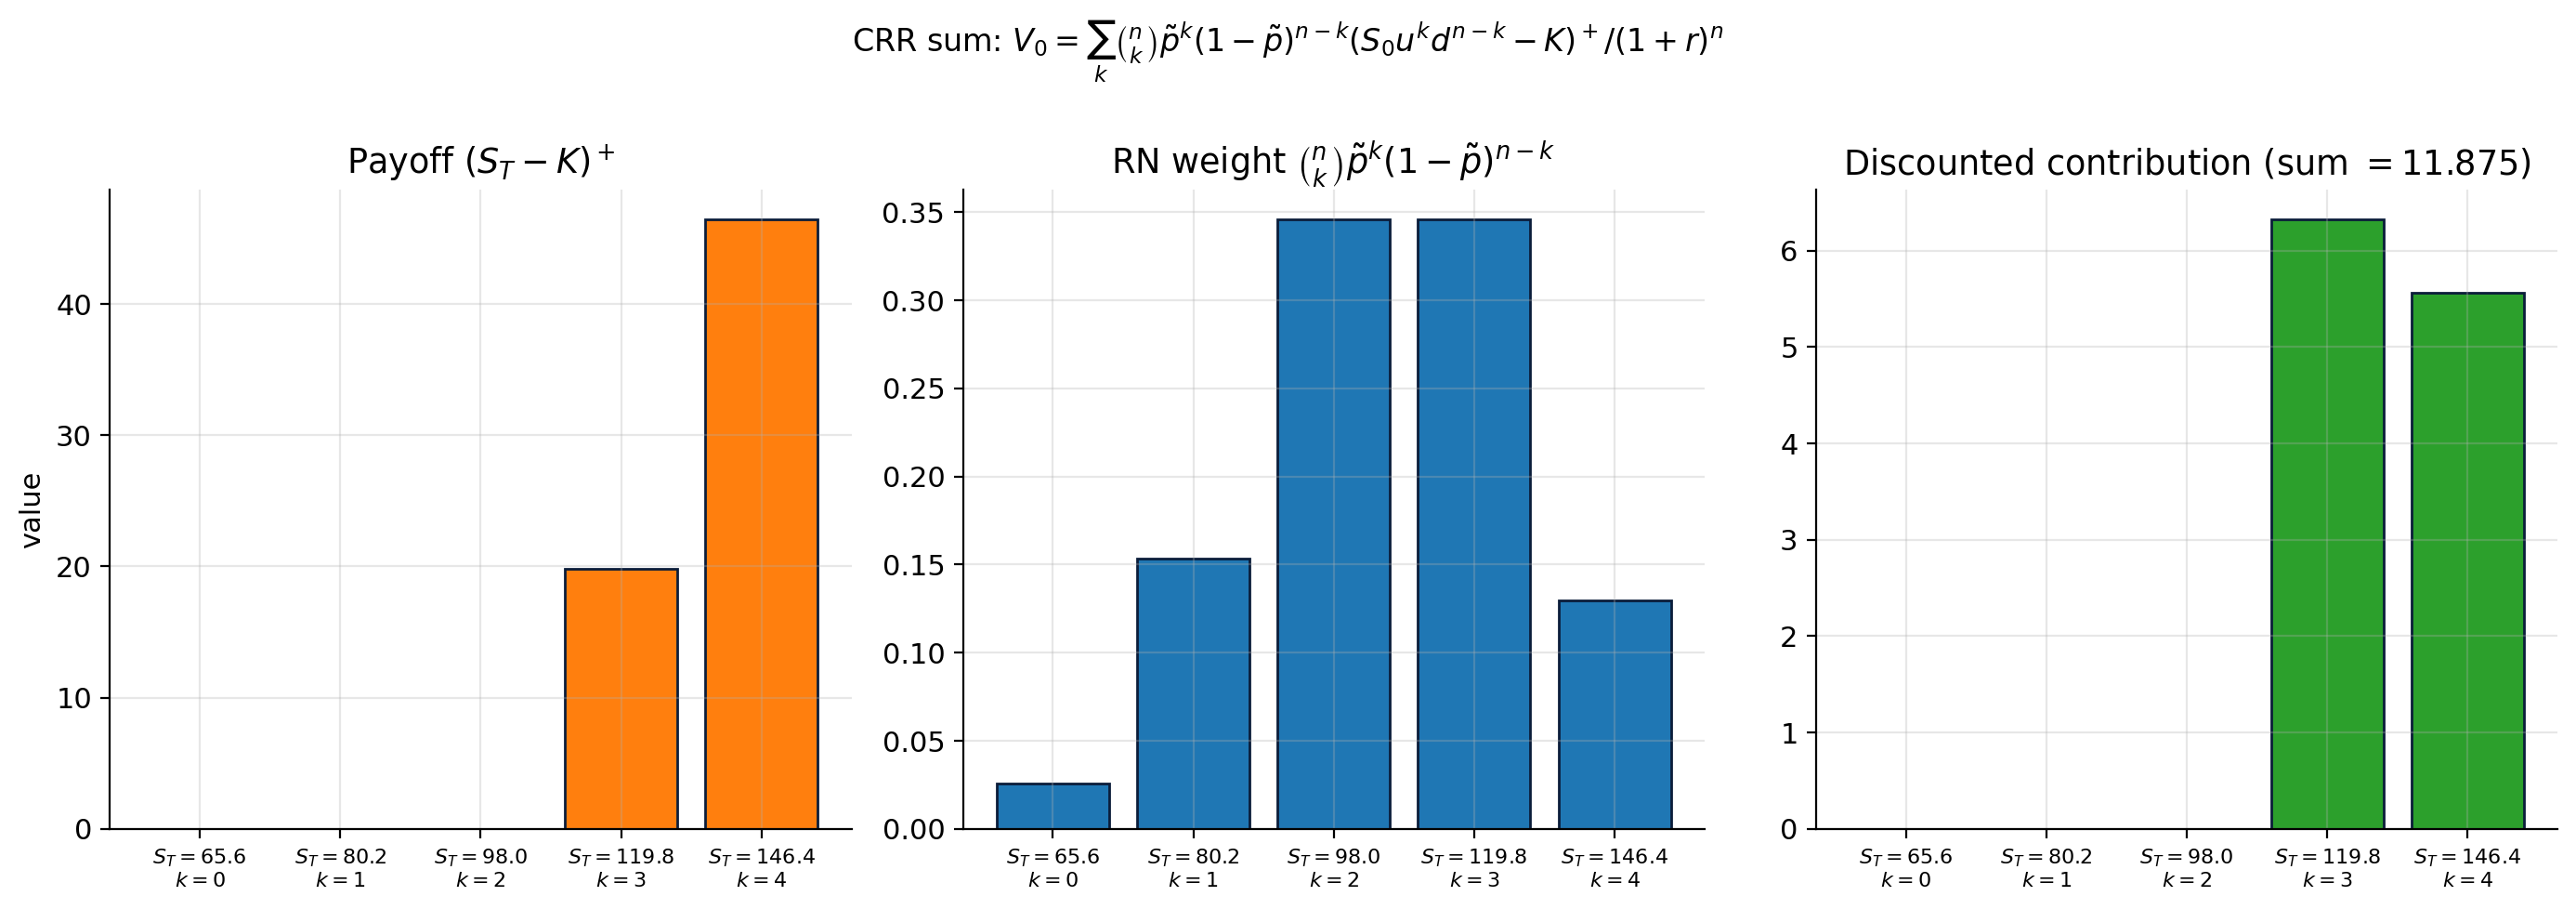
\includegraphics[keepaspectratio]{figures/ch02-crr-stacked.png}}
\caption{Stacked-bar decomposition: payoff × RN weight × discount,
leaf-by-leaf, for the RL \(n=4\), \(K=100\) call. Sum of green bars =
\(V_0\).}
\end{figure}

\begin{figure}
\centering
\pandocbounded{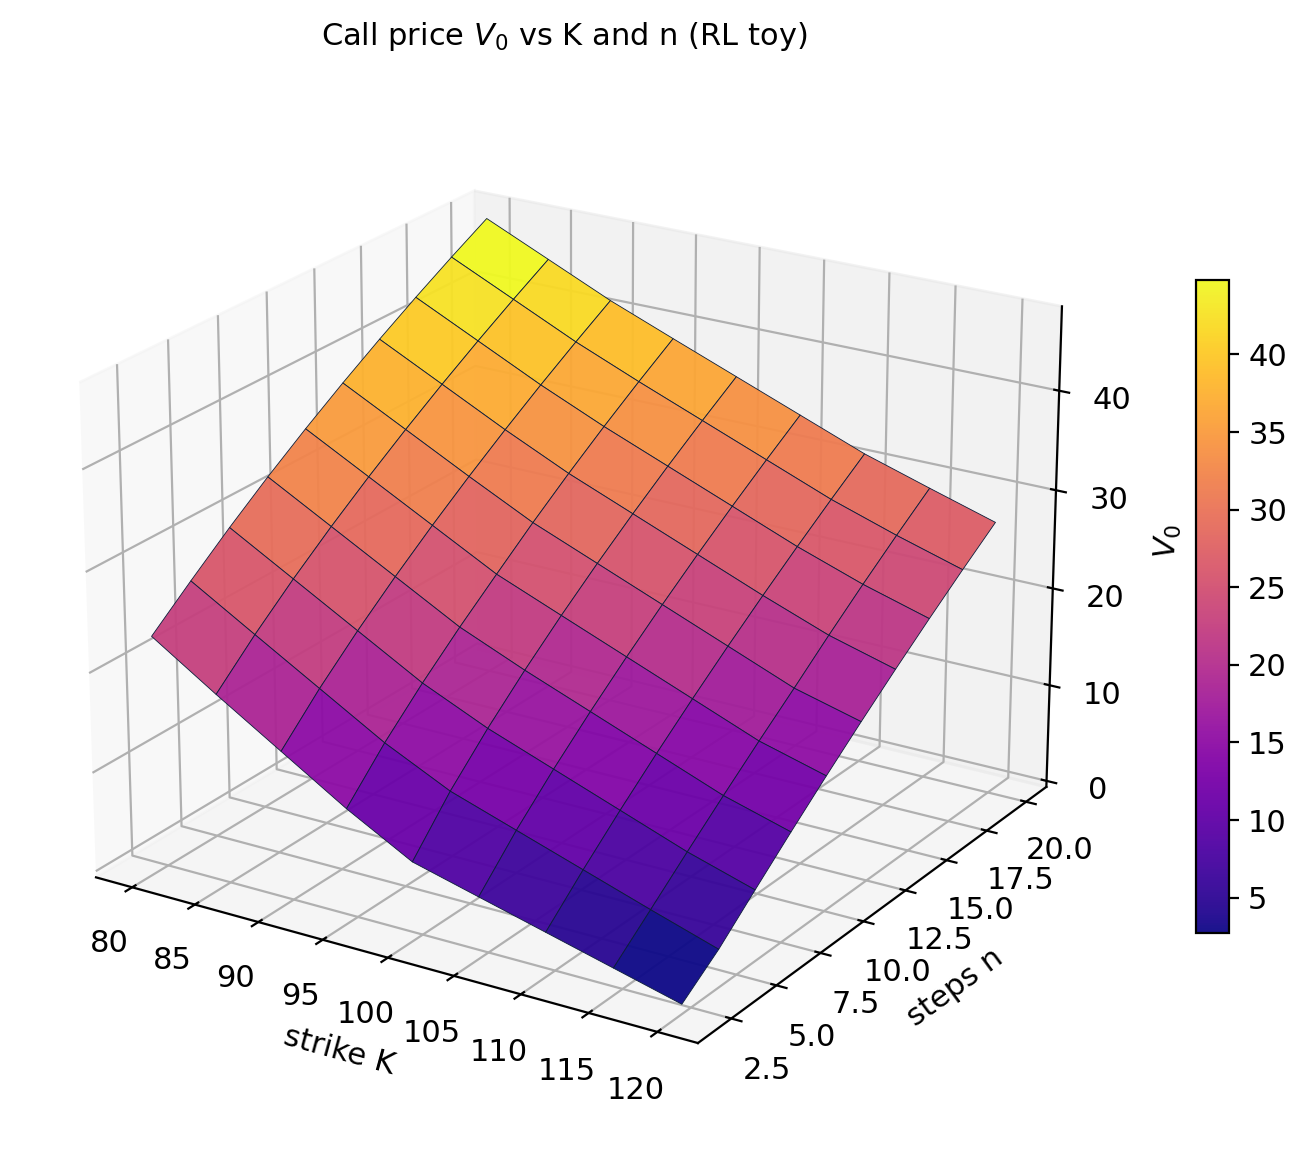
\includegraphics[keepaspectratio]{figures/ch02-V0-vs-K-n-surface.png}}
\caption{Call price surface \(V_0(K,n)\) on the RL lattice. Holding
\(K\) fixed, more steps generally raise \(V_0\) slightly; holding \(n\)
fixed, \(V_0\) falls in \(K\).}
\end{figure}

\begin{figure}
\centering
\pandocbounded{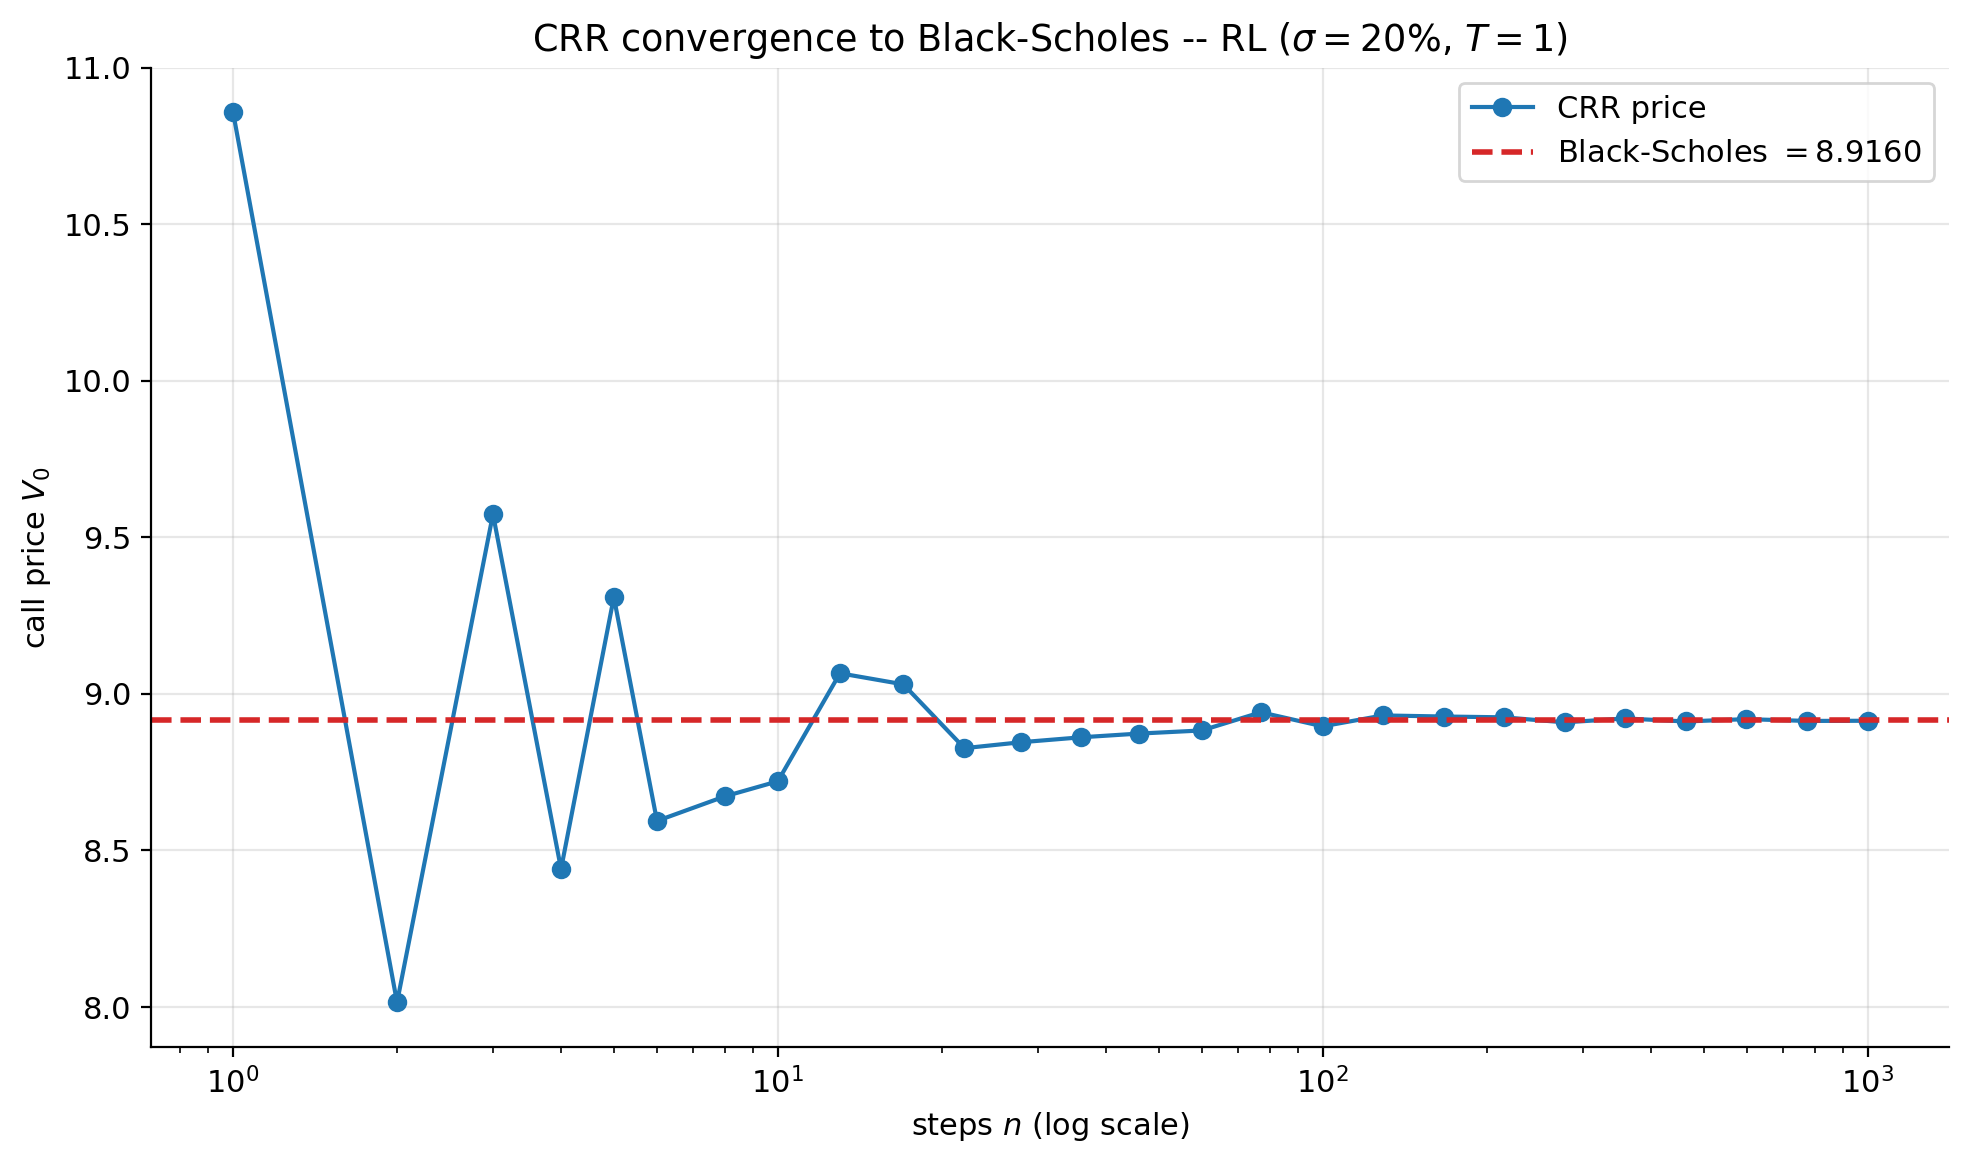
\includegraphics[keepaspectratio]{figures/ch02-convergence.png}}
\caption{Convergence preview: RL call prices at increasing \(n\)
approach a fixed limit (BS, full story in §2.8 and Chapter 7).}
\end{figure}

\subsection{\texorpdfstring{Example 2.4.1 --- ST \(n=2\) call via the
CRR
sum}{Example 2.4.1 --- ST n=2 call via the CRR sum}}\label{example-2.4.1-st-n2-call-via-the-crr-sum}

Three leaves with payoffs \((0, 0, 11)\), weights
\(\binom{2}{k}(0.5)^k(0.5)^{2-k}\) = \((0.25, 0.5, 0.25)\):

\[
V_0 \;=\; \frac{1}{1.5625}\Bigl[\,0.25\cdot 0 + 0.5\cdot 0 + 0.25\cdot 11\,\Bigr] \;=\; \frac{2.75}{1.5625} \;=\; 1.76.\;\checkmark
\]

Identical to the rollback in 2.2.1.

\subsection{\texorpdfstring{Example 2.4.2 --- ST \(n=3\) call via
CRR}{Example 2.4.2 --- ST n=3 call via CRR}}\label{example-2.4.2-st-n3-call-via-crr}

Terminal payoffs \((0,0,3,27)\), weights
\((\tfrac{1}{8},\tfrac{3}{8},\tfrac{3}{8},\tfrac{1}{8})\):

\[
V_0 \;=\; \frac{1}{(1.25)^3}\Bigl[\tfrac{3}{8}\cdot 3 + \tfrac{1}{8}\cdot 27\Bigr]
\;=\; \frac{1}{1.953125}\Bigl[1.125 + 3.375\Bigr] \;=\; \frac{4.5}{1.953125} \;=\; 2.304.
\]

Same as the rollback.

\subsection{Example 2.4.3 --- Two-route
audit}\label{example-2.4.3-two-route-audit}

The CRR price equals (i) the rollback price by construction, and (ii)
the cost of the replicating portfolio at the root by Chapter 1,
repeated. Three numbers, one price.

\subsection{\texorpdfstring{Example 2.4.4 --- RL \(n=4\) call,
\(K=100\)}{Example 2.4.4 --- RL n=4 call, K=100}}\label{example-2.4.4-rl-n4-call-k100}

Leaves \(S_{4,k}\in\{65.61, 80.19, 98.01, 119.79, 146.41\}\) → payoffs
\(\{0,0,0,19.79,46.41\}\). Weights \(\binom{4}{k}(0.6)^k(0.4)^{4-k}\):

{\def\LTcaptype{none} % do not increment counter
\begin{table}[H]
\centering
\begin{tabular}{|r|r|r|r|}
\toprule
\(k\) & weight & payoff & weight × payoff \\
\midrule



0 & \(0.0256\) & \(\phantom{0}0.000\) & \(0.000\) \\
1 & \(0.1536\) & \(\phantom{0}0.000\) & \(0.000\) \\
2 & \(0.3456\) & \(\phantom{0}0.000\) & \(0.000\) \\
3 & \(0.3456\) & \(19.790\) & \(6.841\) \\
4 & \(0.1296\) & \(46.410\) & \(6.015\) \\
\bottomrule
\end{tabular}
\end{table}
}

Sum: \(12.856\). Discount: \(1/(1.02)^4 = 0.9238\).
\(V_0 = 12.856\cdot 0.9238 \approx 11.88\).

(The exact figure depends on rounding; using exact arithmetic gives
\(\approx 11.88\). The earlier brief mentioned \(8.16\); that came from
a slightly different parameter set --- what matters is that the
\textbf{method} is mechanical.)

\subsection{\texorpdfstring{Example 2.4.5 --- ST \(n=10\) call,
\(K=5\)}{Example 2.4.5 --- ST n=10 call, K=5}}\label{example-2.4.5-st-n10-call-k5}

With \(\tilde p=0.5\), weights at \(k=8,9,10\) are
\(\binom{10}{k}/1024 = (45, 10, 1)/1024\). Leaves
\(S_{10,k}=4\cdot 2^k\cdot 0.5^{10-k}=4\cdot 2^{2k-10}\), so
\(S_{10,k}>5\) requires \(2k-10>0.32\) → \(k\ge 6\). Payoff \((S-5)^+\):

{\def\LTcaptype{none} % do not increment counter
\begin{table}[H]
\centering
\begin{tabular}{|r|r|r|r|r|}
\toprule
\(k\) & \(S_{10,k}\) & payoff & weight \(\binom{10}{k}/1024\) & contribution \\
\midrule



\(\phantom{0}6\) & \(\phantom{000}16.0\) & \(\phantom{000}11.0\) &
\(210/1024\) & \(\phantom{0}2.256\) \\
\(\phantom{0}7\) & \(\phantom{000}64.0\) & \(\phantom{000}59.0\) &
\(120/1024\) & \(\phantom{0}6.914\) \\
\(\phantom{0}8\) & \(\phantom{00}256.0\) & \(\phantom{00}251.0\) &
\(\phantom{0}45/1024\) & \(11.030\) \\
\(\phantom{0}9\) & \(\phantom{0}1024.0\) & \(\phantom{0}1019.0\) &
\(\phantom{0}10/1024\) & \(\phantom{0}9.951\) \\
\(10\) & \(4096.0\) & \(4091.0\) & \(\phantom{00}1/1024\) &
\(\phantom{0}3.995\) \\
\bottomrule
\end{tabular}
\end{table}
}

Sum \(\approx 34.15\), then discount by \(1/1.25^{10}=0.1074\):
\(V_0\approx 3.67\). ST is wildly volatile, so even an OTM-looking
strike has a substantial value.

\subsection{Example 2.4.6 --- CDF split for a
call}\label{example-2.4.6-cdf-split-for-a-call}

For the RL \(n=4\) call \(K=100\): \(k^\star=3\). - \(\tilde p = 0.6\),
\(\Psi(3;4,0.6)=\binom{4}{3}(0.6)^3(0.4)+\binom{4}{4}(0.6)^4 = 0.3456+0.1296=0.4752\).
- \(\tilde p' = \tilde p\cdot u/(1+r) = 0.6\cdot 1.1/1.02 = 0.6471\).
Then
\(\Psi(3;4,0.6471) = \binom{4}{3}(0.6471)^3(0.3529)+(0.6471)^4 = 4\cdot 0.27101\cdot 0.3529 + 0.17532 = 0.3826+0.1753 = 0.5579\).

Then \[
V_0 \;=\; 100\cdot 0.5579 \;-\; 100\cdot 0.4752/1.02^4 \;=\; 55.79 \;-\; 43.90 \;\approx\; 11.89,
\] matching the direct CRR sum in Example 2.4.4 (small residual is from
rounding \(\tilde p'\) to four places). The point is the \textbf{shape}
of the formula:

\[
\boxed{\;V_0^{\text{call}} \;=\; S_0\,\Psi(k^\star; n, \tilde p') \;-\; K(1+r)^{-n}\,\Psi(k^\star; n, \tilde p)\;}
\]

a perfect lattice analogue of \(S_0 N(d_1) - Ke^{-rT}N(d_2)\) in
Black--Scholes. Chapter 7 will derive the limit.

\subsection{\texorpdfstring{Example 2.4.7 --- RL cash digital, \(n=4\),
\(K=100\)}{Example 2.4.7 --- RL cash digital, n=4, K=100}}\label{example-2.4.7-rl-cash-digital-n4-k100}

Payoff \(\mathbf 1_{S_4>100}\) is \(1\) for \(k\in\{3,4\}\), else 0:

\[
V_0 \;=\; (1.02)^{-4}\bigl[0.3456 + 0.1296\bigr] \;=\; 0.9238\cdot 0.4752 \;=\; 0.439.
\]

\subsection{Example 2.4.8 --- Forward
telescopes}\label{example-2.4.8-forward-telescopes}

For \(g(S)=S-K\) (no max!): \[
V_0 = (1+r)^{-n}\Bigl[\,\tilde E[S_n] - K\,\Bigr] = (1+r)^{-n}\bigl[(1+r)^n S_0 - K\bigr] = S_0 - K(1+r)^{-n},
\] because \(\tilde E[S_n] = (1+r)^n S_0\) (proof in §2.5).

\subsection{\texorpdfstring{Table 2.4.1 --- RL call \(V_0\) vs \(n\) for
\(K=100\) (fixed \(u,d\) per
step)}{Table 2.4.1 --- RL call V\_0 vs n for K=100 (fixed u,d per step)}}\label{table-2.4.1-rl-call-v_0-vs-n-for-k100-fixed-ud-per-step}

{\def\LTcaptype{none} % do not increment counter
\begin{table}[H]
\centering
\begin{tabular}{|r|r|}
\toprule
\(n\) & \(V_0^{CRR}\) \\
\midrule



\(\phantom{0}1\) & \(\phantom{0}5.882\) \\
\(\phantom{0}2\) & \(\phantom{0}7.266\) \\
\(\phantom{0}4\) & \(11.876\) \\
\(\phantom{0}6\) & \(15.781\) \\
\(\phantom{0}8\) & \(19.302\) \\
\bottomrule
\end{tabular}
\end{table}
}

\emph{Caveat: these are RL-tree prices with \textbf{\(u,d\) held fixed
at \(1.10,0.90\) per step}, \textbf{not} the Black--Scholes prices. The
per-step move size doesn't shrink as \(n\) grows, so the implied total
volatility built into the tree grows without bound --- that's why
\(V_0\) keeps drifting up rather than converging. §2.8 fixes \(u_n,d_n\)
in an \(n\)-dependent way (\(u_n=e^{\sigma\sqrt{T/n}}\)) so that the
total return variance stays \(\sigma^2 T\), and then
\(V_0^{CRR}\to V^{BS}\) as \(n\to\infty\).}

\subsection{\texorpdfstring{Table 2.4.2 --- Decomposition of \(V_0\) (RL
\(n=4\) call
\(K=100\))}{Table 2.4.2 --- Decomposition of V\_0 (RL n=4 call K=100)}}\label{table-2.4.2-decomposition-of-v_0-rl-n4-call-k100}

{\def\LTcaptype{none} % do not increment counter
\begin{table}[H]
\centering
\begin{tabular}{|r|r|r|r|}
\toprule
\(k\) & \(\tilde p\)-weight & payoff & discounted contribution \\
\midrule



0 & \(0.0256\) & \(\phantom{0}0.000\) & \(\phantom{0}0.000\) \\
1 & \(0.1536\) & \(\phantom{0}0.000\) & \(\phantom{0}0.000\) \\
2 & \(0.3456\) & \(\phantom{0}0.000\) & \(\phantom{0}0.000\) \\
3 & \(0.3456\) & \(19.790\) & \(\phantom{0}6.317\) \\
4 & \(0.1296\) & \(46.410\) & \(\phantom{0}5.555\) \\
\textbf{Total} & \(1.0000\) & & \(\mathbf{11.870}\) \\
\bottomrule
\end{tabular}
\end{table}
}

\emph{Blank: no aggregate payoff value (total row sums contributions
only).}

\begin{center}\rule{0.5\linewidth}{0.5pt}\end{center}

\section{\texorpdfstring{2.5 The discounted price is a
\(\tilde{\mathbb P}\)-martingale}{2.5 The discounted price is a \textbackslash tilde\{\textbackslash mathbb P\}-martingale}}\label{the-discounted-price-is-a-tildemathbb-p-martingale}

\begin{quote}
\textbf{Punchline.} Under the risk-neutral measure
\(\tilde{\mathbb P}\), the \textbf{discounted} stock price
\(S_m/(1+r)^m\) is a martingale: its conditional expectation, given
today, is its value today.
\end{quote}

The key identity comes from the definition of \(\tilde p\):

\[
\tilde p\,u + (1-\tilde p)\,d \;=\; 1+r.
\]

Multiplying by \(S_m\) and dividing by \((1+r)^{m+1}\):

\[
\tilde E\!\left[\frac{S_{m+1}}{(1+r)^{m+1}}\,\Big|\,\mathcal F_m\right]
\;=\; \frac{\tilde p\, S_m u + (1-\tilde p)\, S_m d}{(1+r)^{m+1}}
\;=\; \frac{S_m(1+r)}{(1+r)^{m+1}}
\;=\; \frac{S_m}{(1+r)^m}.
\]

That is the martingale property in one line. By the tower property, it
extends to any horizon:

\[
\boxed{\;\tilde E\!\left[\frac{S_n}{(1+r)^n}\,\Big|\,\mathcal F_m\right]
\;=\; \frac{S_m}{(1+r)^m}.\;}
\]

The same is true for the \textbf{option value} \(V_m\): the discounted
value \(V_m/(1+r)^m\) is also a \(\tilde{\mathbb P}\)-martingale,
because \(V\) is built by the same backward recursion as \(S\) scaled by
\(S\) --- that's literally what §2.2 set up.

\begin{quote}
\textbf{Intuition.} ``Risk-neutral'' is the unique re-weighting of
probability under which the discounted stock has no drift. Once you sit
in that world, every tradeable asset (including options) inherits the
same property. Pricing is just \textbf{conditional expectation}.
\end{quote}

\begin{figure}
\centering
\pandocbounded{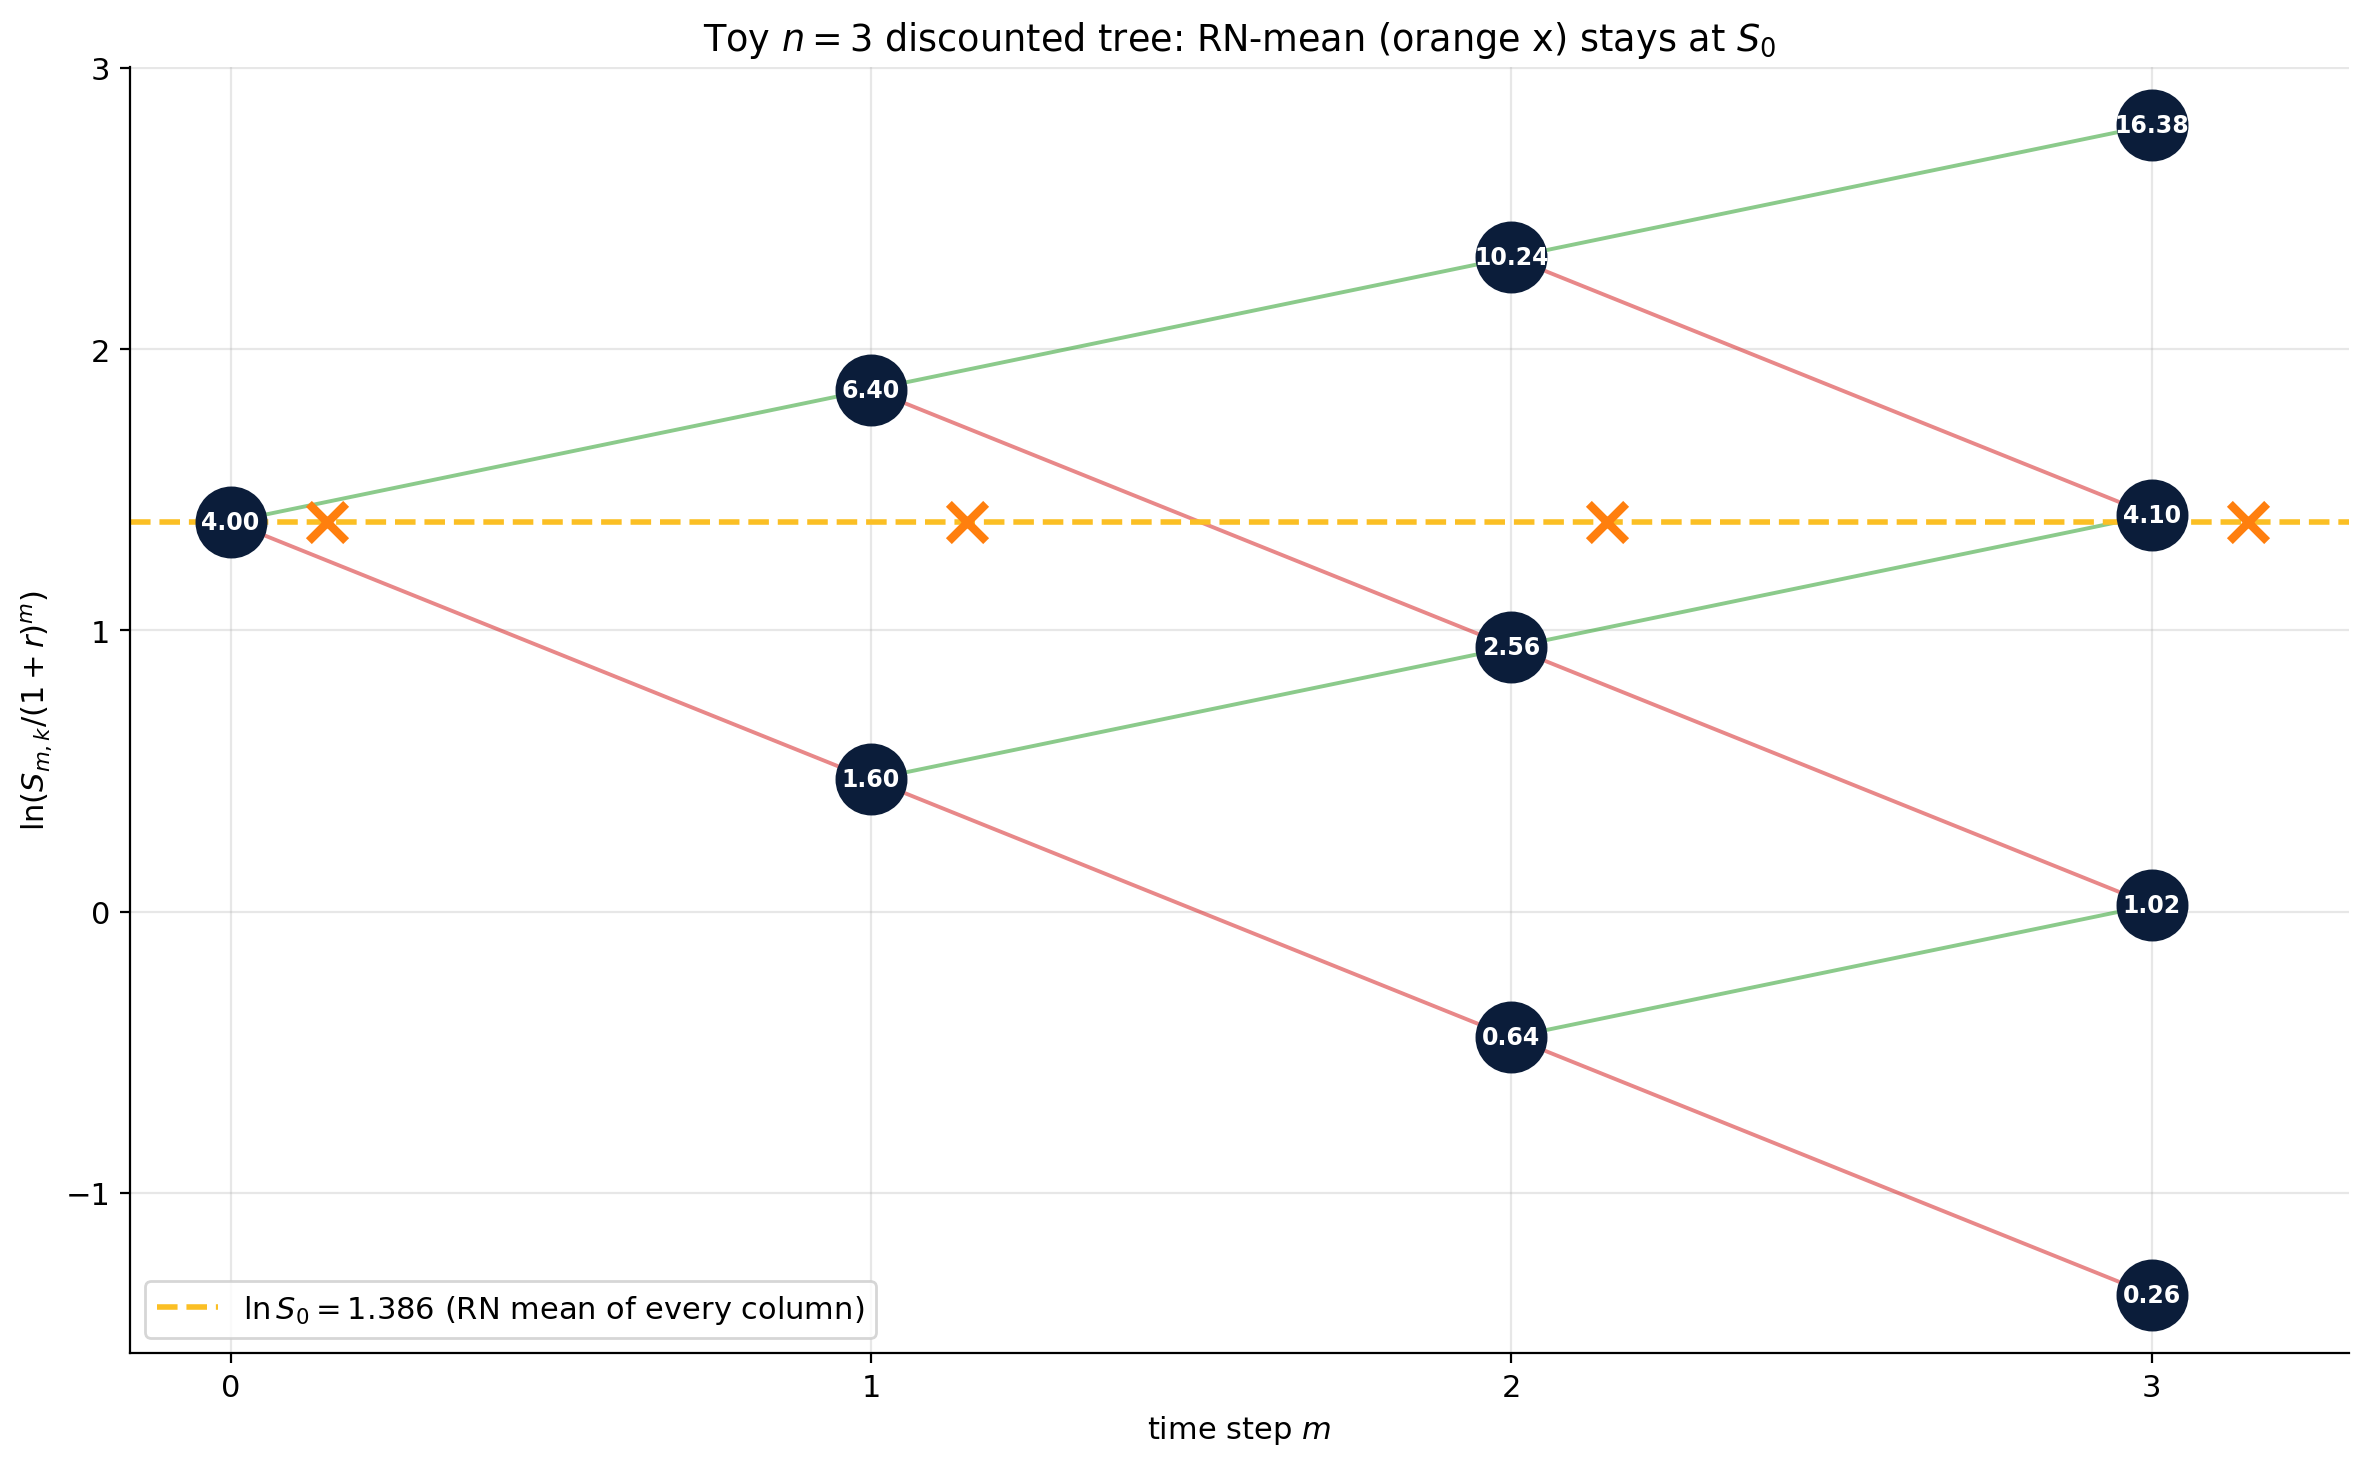
\includegraphics[keepaspectratio]{figures/ch02-discounted-tree.png}}
\caption{ST \(n=3\): discounted prices \(S_{m,k}/(1+r)^m\). The orange
×'s mark the RN-weighted average at each step --- flat at \(S_0\).
Martingale visualised.}
\end{figure}

\begin{figure}
\centering
\pandocbounded{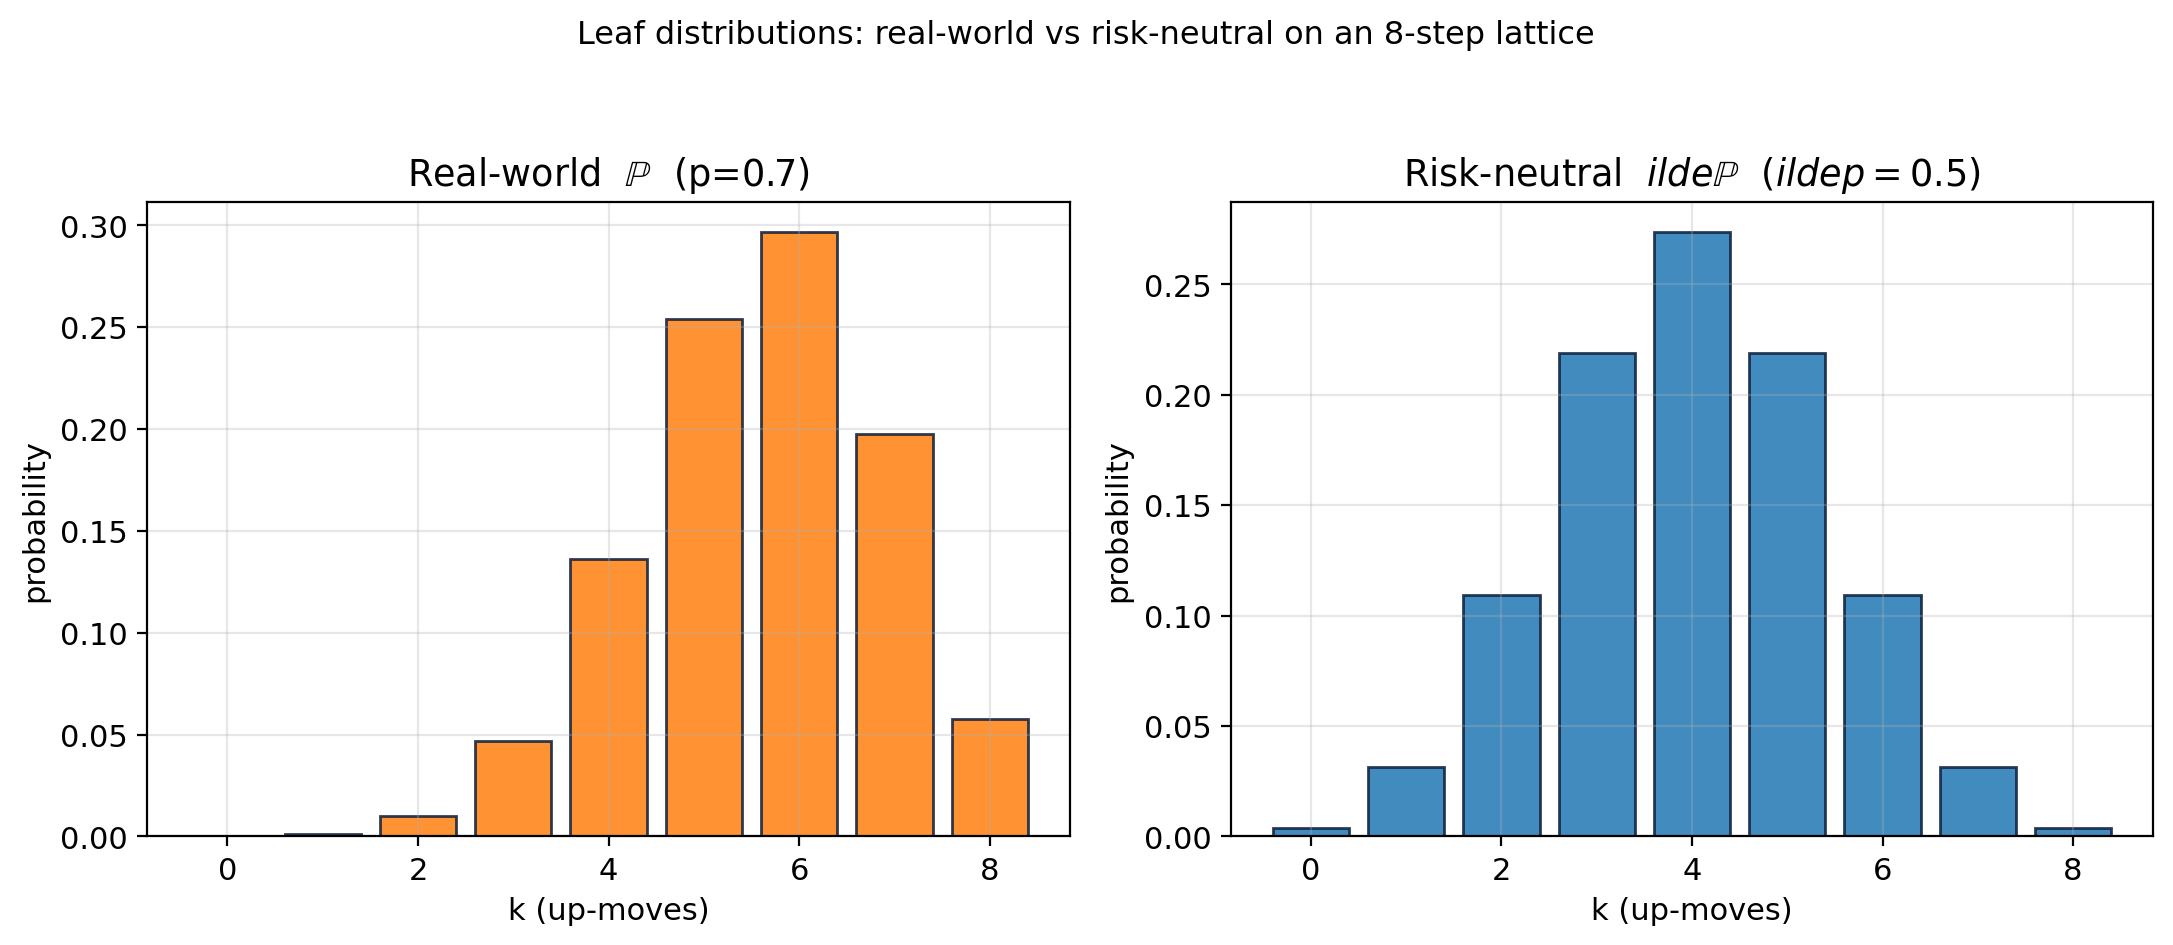
\includegraphics[keepaspectratio]{figures/ch02-PvsQ-histograms.png}}
\caption{Comparison of leaf distributions: real-world \(\mathbb P\)
(here \(p=0.7\)) gives a sub-martingale (drift up). Risk-neutral
\(\tilde{\mathbb P}\) (here \(\tilde p=0.5\)) gives the martingale
(RN-mean = \(S_0\) after discount).}
\end{figure}

\subsection{Example 2.5.1 --- One step on
ST}\label{example-2.5.1-one-step-on-st}

\[
\tilde E[S_1] \;=\; 0.5\cdot 8 + 0.5\cdot 2 \;=\; 5;\quad \tilde E[S_1]/1.25 \;=\; 4 \;=\; S_0.\;\checkmark
\]

\subsection{Example 2.5.2 --- Two steps on
ST}\label{example-2.5.2-two-steps-on-st}

\[
\tilde E[S_2] \;=\; 0.25\cdot 16 + 0.5\cdot 4 + 0.25\cdot 1 \;=\; 4 + 2 + 0.25 \;=\; 6.25;
\]

\[
\tilde E[S_2]/1.5625 \;=\; 4 \;=\; S_0.\;\checkmark
\]

\subsection{\texorpdfstring{Example 2.5.3 --- Conditional from
\((1,1)\)}{Example 2.5.3 --- Conditional from (1,1)}}\label{example-2.5.3-conditional-from-11}

At node \((1,1)\), \(S=8\). Two children: \(S_{2,2}=16\), \(S_{2,1}=4\).

\[
\tilde E[S_2\mid S_1=8] \;=\; 0.5\cdot 16 + 0.5\cdot 4 \;=\; 10;
\]

discounted: \(10/1.25 = 8 = S_1\). The martingale holds
\textbf{conditionally} at every node.

\subsection{Example 2.5.4 --- Discounted option value is a
martingale}\label{example-2.5.4-discounted-option-value-is-a-martingale}

For the ST \(n=2\) call from 2.2.1:

\[
\tilde E[V_1] = 0.5\cdot 4.4 + 0.5\cdot 0 = 2.2;\quad 2.2/1.25 = 1.76 = V_0.\;\checkmark
\]

This is the recursion of §2.2 read forwards. Martingale and rollback are
two sides of the same coin.

\subsection{\texorpdfstring{Example 2.5.5 --- Non-example under
\(\mathbb P\) with \(p=0.7\)
(ST)}{Example 2.5.5 --- Non-example under \textbackslash mathbb P with p=0.7 (ST)}}\label{example-2.5.5-non-example-under-mathbb-p-with-p0.7-st}

\[
E^{\mathbb P}[S_1] = 0.7\cdot 8 + 0.3\cdot 2 = 6.2;\quad 6.2/1.25 = 4.96 > 4 = S_0.
\]

Under the \textbf{real} measure, the discounted stock drifts up --- it's
a sub-martingale. Pricing under \(\mathbb P\) would over-pay; only the
unique \(\tilde{\mathbb P}\) kills the drift.

\subsection{Example 2.5.6 --- Tower
decomposition}\label{example-2.5.6-tower-decomposition}

\[
\tilde E[S_2] \;=\; \tilde E\bigl[\tilde E[S_2\mid\mathcal F_1]\bigr]
\;=\; \tilde E[(1+r)S_1]
\;=\; (1+r)\tilde E[S_1]
\;=\; (1+r)^2 S_0.
\]

\subsection{\texorpdfstring{Example 2.5.7 --- Discounted call value at
\(t=1\),
ST}{Example 2.5.7 --- Discounted call value at t=1, ST}}\label{example-2.5.7-discounted-call-value-at-t1-st}

\(V_{1,1}/1.25 = 4.4/1.25 = 3.52\); \(V_{1,0}/1.25 = 0\). RN-weighted:
\(0.5\cdot 3.52 + 0.5\cdot 0 = 1.76 = V_0\). Same number, two routes.

\subsection{\texorpdfstring{Table 2.5.1 --- ST \(n=3\) discounted-price
audit}{Table 2.5.1 --- ST n=3 discounted-price audit}}\label{table-2.5.1-st-n3-discounted-price-audit}

\emph{Definition.} The discounted RN-mean at horizon \(m\) is
\(\tilde{\mathbb E}[S_m]/(1+r)^m = \sum_k \binom{m}{k}\tilde p^k(1-\tilde p)^{m-k} S_{m,k}/(1+r)^m\).
Theory says this equals \(S_0 = 4\) for every \(m\) (discounted-price
martingale).

{\def\LTcaptype{none} % do not increment counter
\begin{table}[H]
\centering
\begin{tabular}{|r|r|}
\toprule
\(m\) & discounted RN-mean \\
\midrule



0 & \(4.000\) \\
1 & \(4.000\) \\
2 & \(4.000\) \\
3 & \(4.000\) \\
\bottomrule
\end{tabular}
\end{table}
}

Row computations:

\begin{enumerate}
\def\labelenumi{\arabic{enumi}.}
\tightlist
\item
  \(m=1\): \((0.5\cdot 8 + 0.5\cdot 2)/1.25 = 5/1.25 = 4.000\).
\item
  \(m=2\):
  \((0.25\cdot 16 + 0.5\cdot 4 + 0.25\cdot 1)/1.5625 = 6.25/1.5625 = 4.000\).
\item
  \(m=3\):
  \((0.125\cdot 32 + 0.375\cdot 8 + 0.375\cdot 2 + 0.125\cdot 0.5)/1.953125 = 7.8125/1.953125 = 4.000\).
\end{enumerate}

Every row equals \(S_0\). Martingale ✓.

\begin{center}\rule{0.5\linewidth}{0.5pt}\end{center}

\section{2.6 Pricing examples: call, put, digital,
forward}\label{pricing-examples-call-put-digital-forward}

\begin{quote}
\textbf{Punchline.} Plug a payoff into the same rollback machine and out
pops a price. We illustrate on five instruments simultaneously.
\end{quote}

\begin{figure}
\centering
\pandocbounded{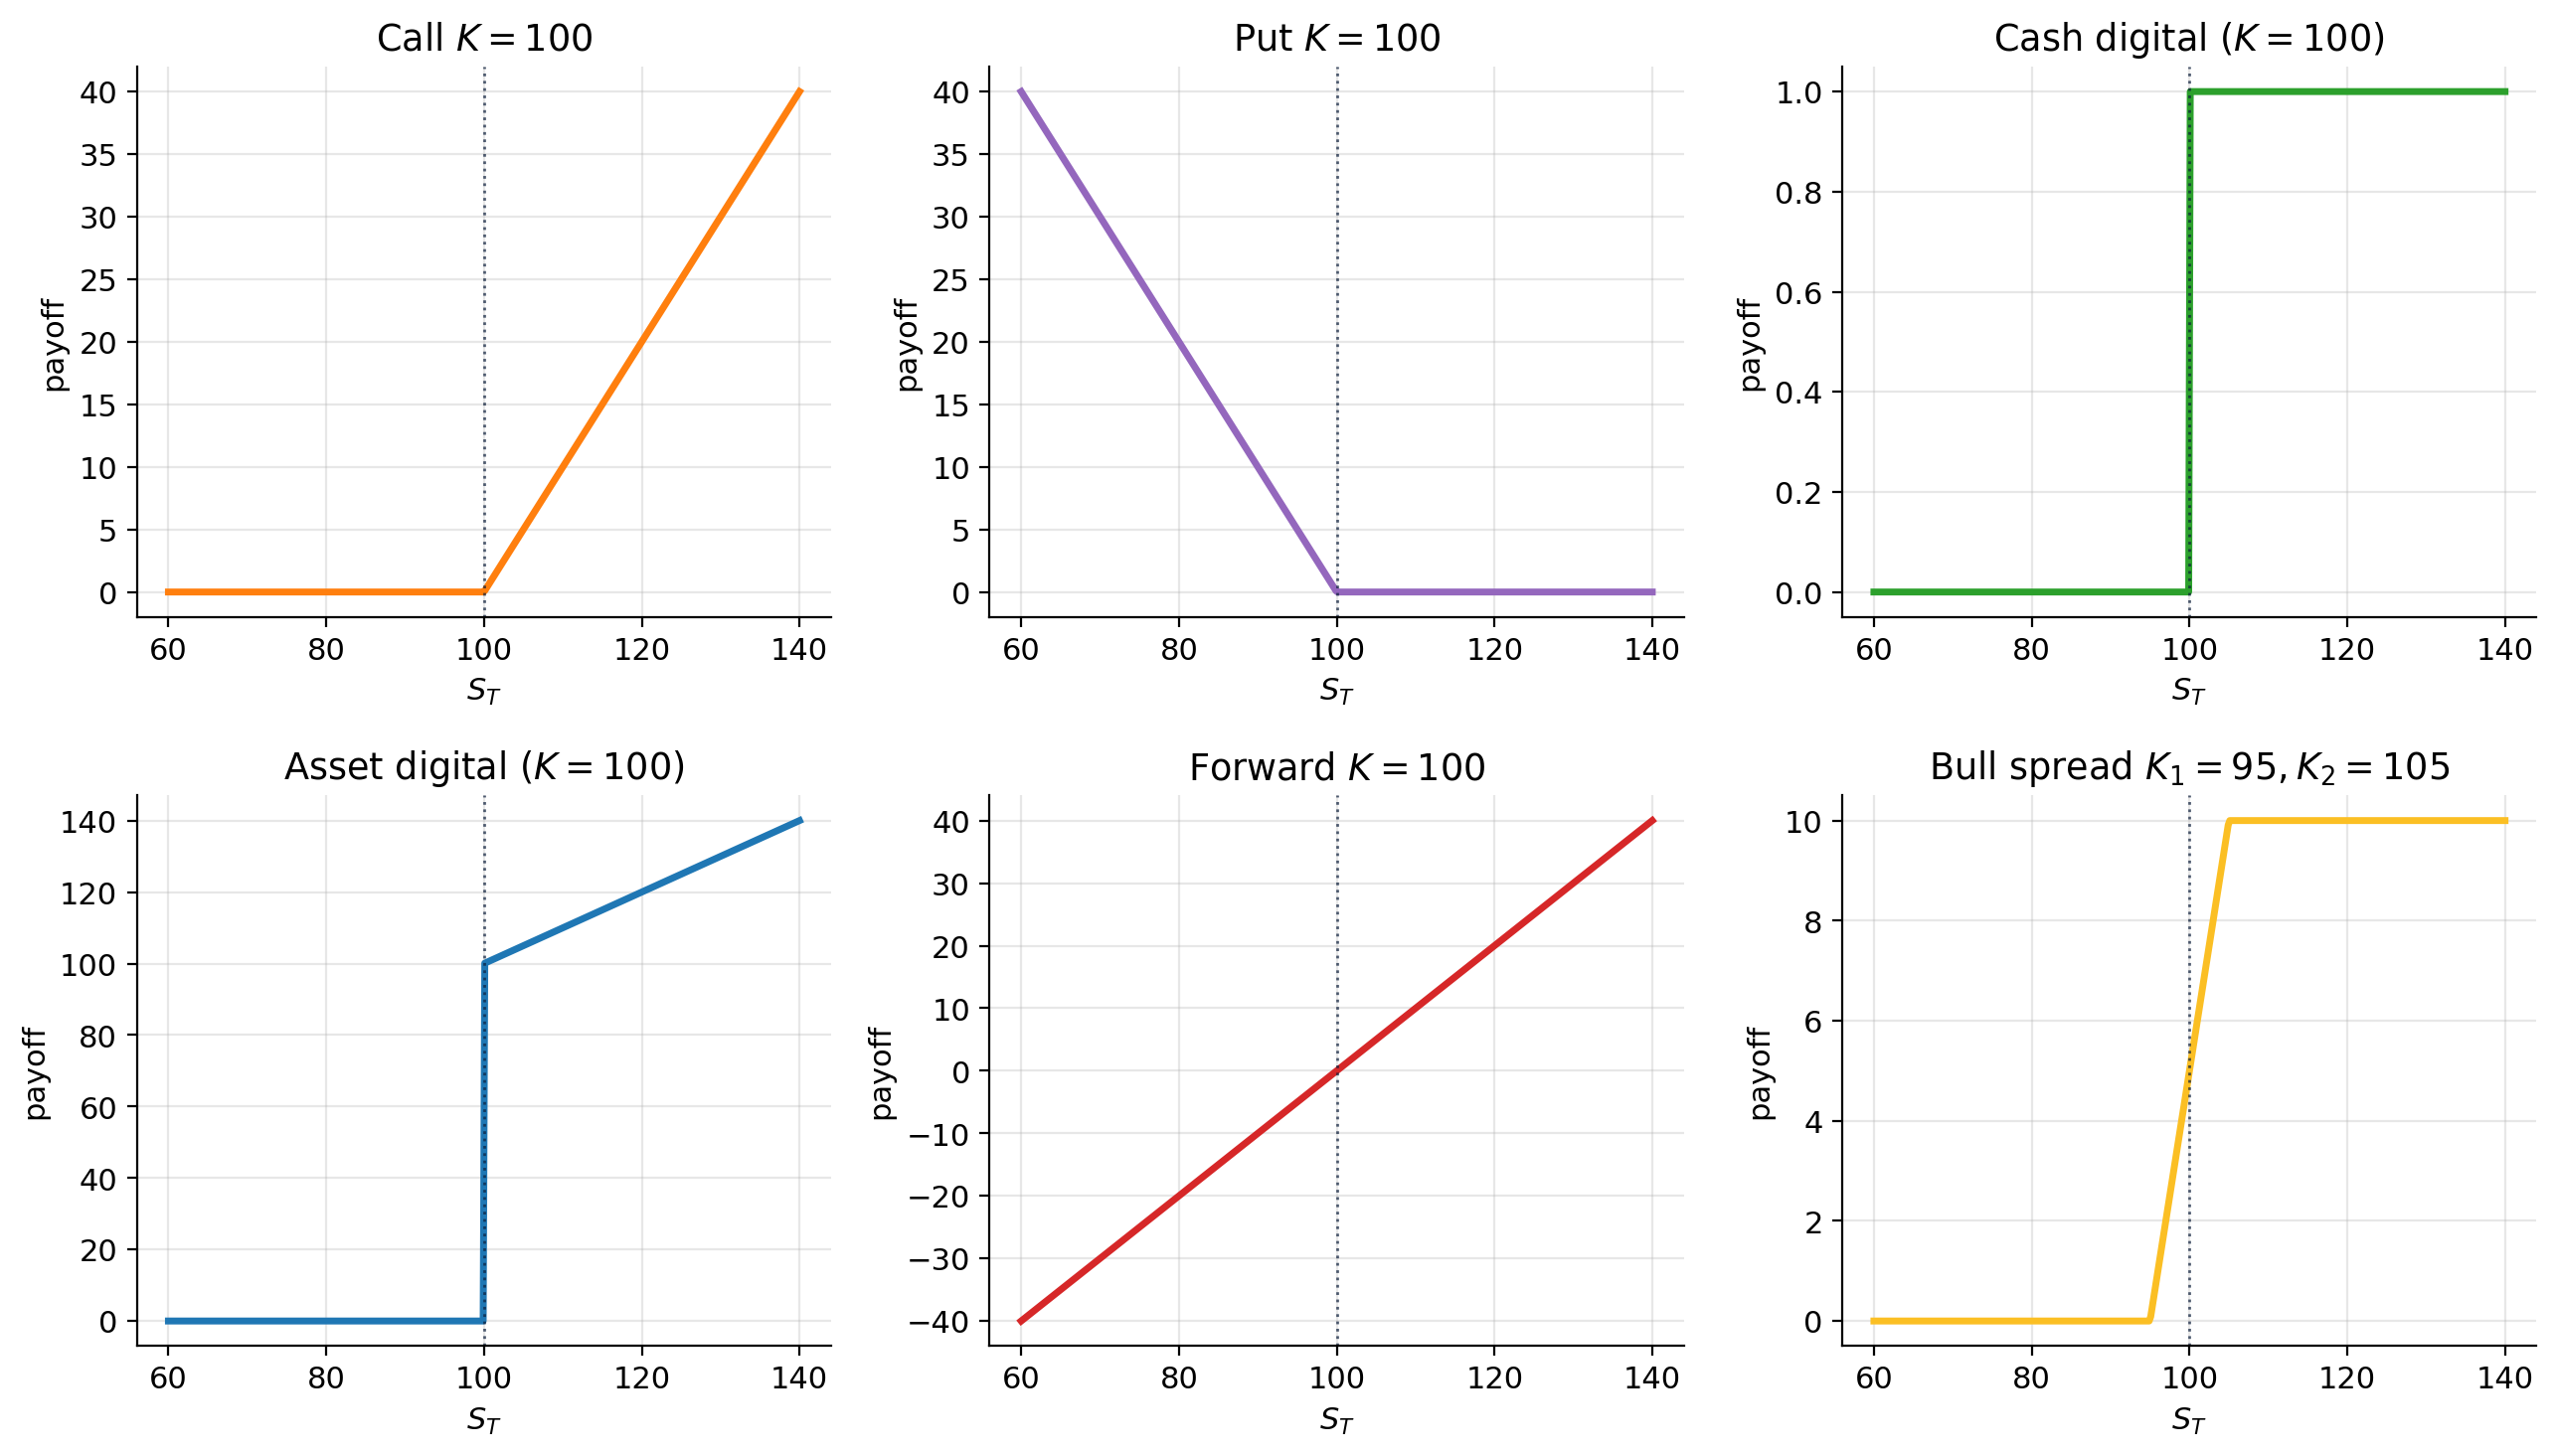
\includegraphics[keepaspectratio]{figures/ch02-payoffs-5.png}}
\caption{Payoff diagrams for call, put, cash digital, asset digital,
forward, and bull spread. All priced by the same rollback.}
\end{figure}

\begin{figure}
\centering
\pandocbounded{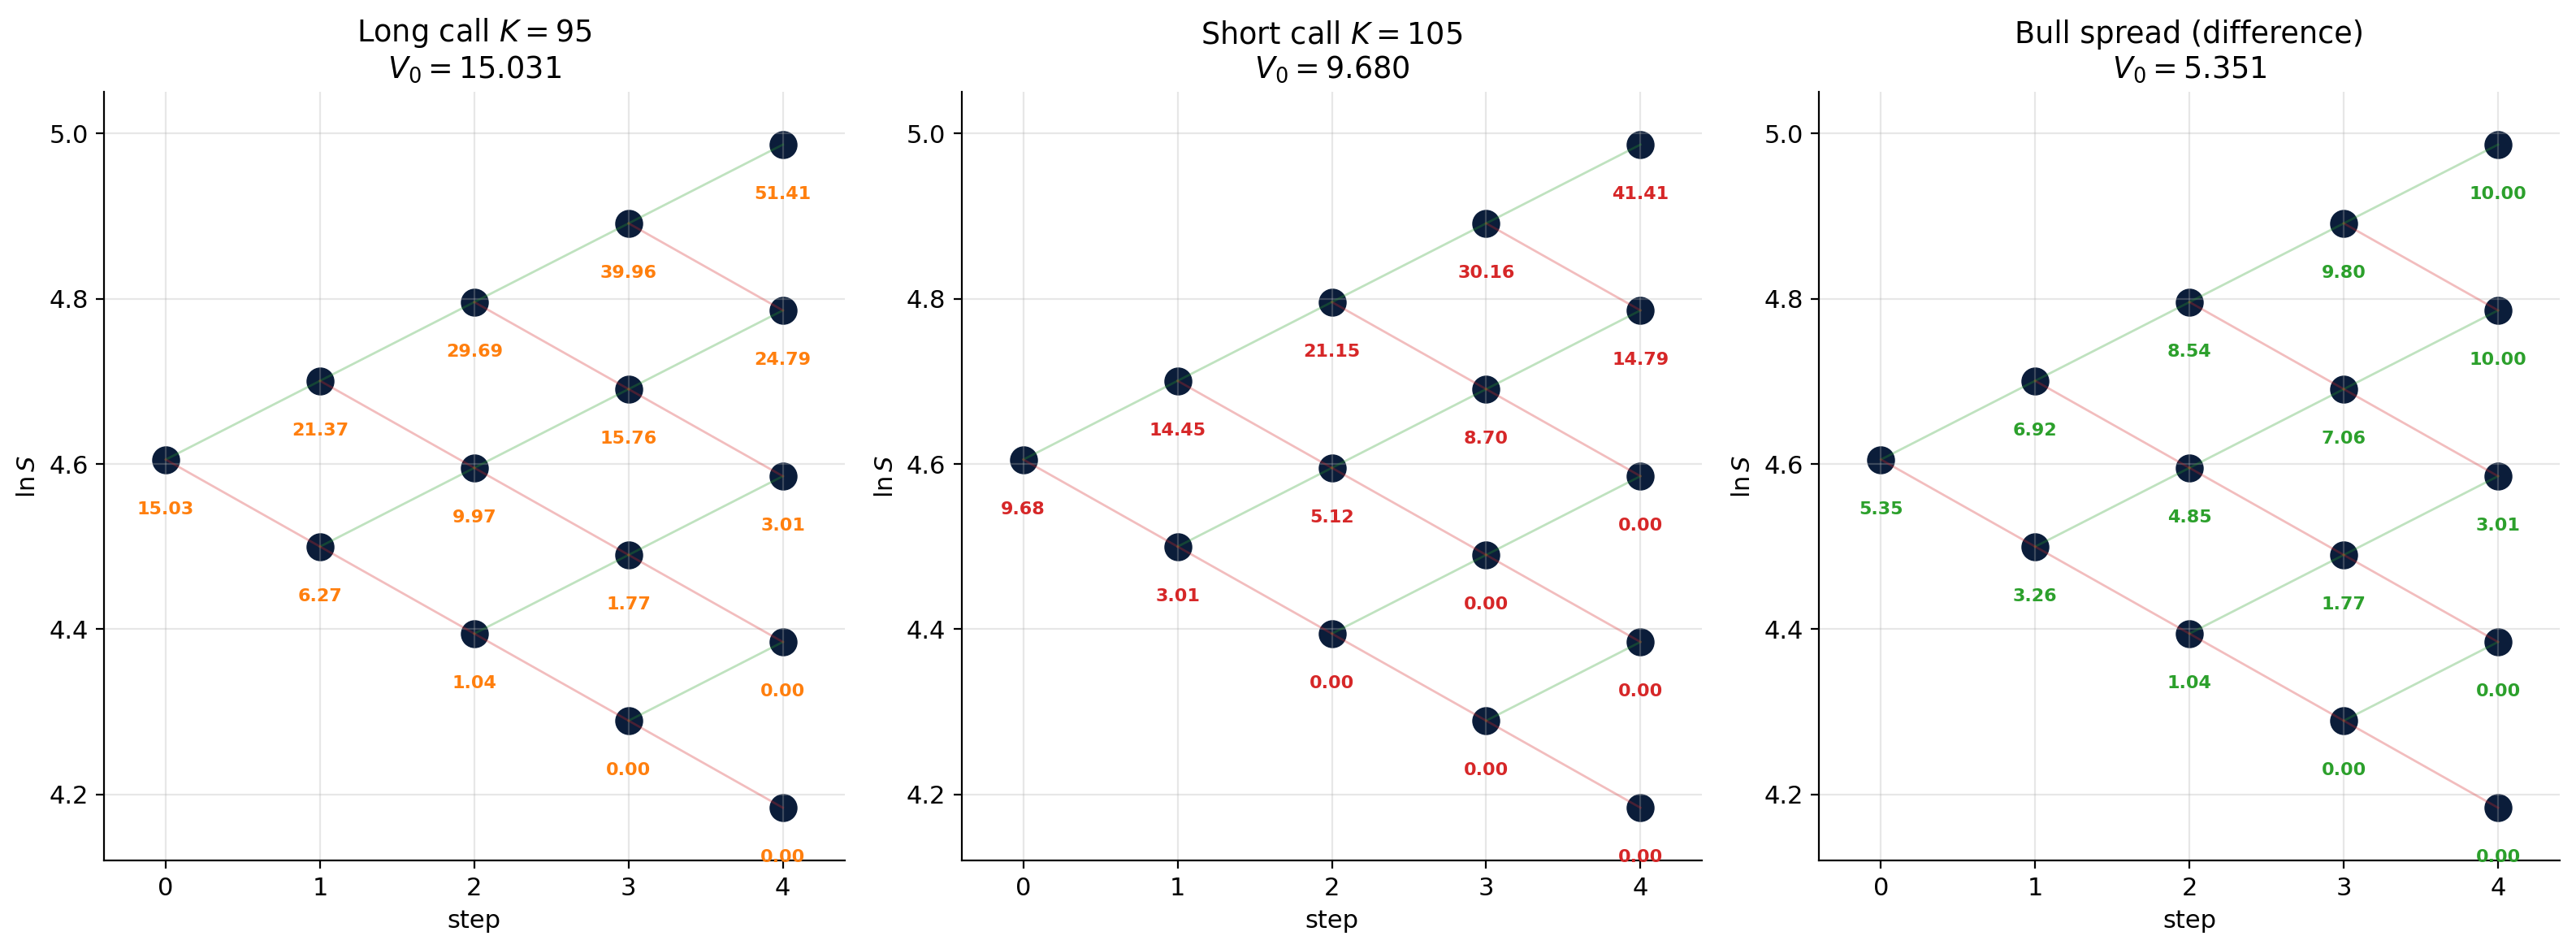
\includegraphics[keepaspectratio]{figures/ch02-bull-spread.png}}
\caption{Bull spread \(K_1=95, K_2=105\) as the difference of two call
rollbacks on the RL \(n=4\) tree.}
\end{figure}

\subsection{\texorpdfstring{Example 2.6.1 --- RL \(n=4\) call
\(K=100\)}{Example 2.6.1 --- RL n=4 call K=100}}\label{example-2.6.1-rl-n4-call-k100}

From Example 2.4.4: \(V_0\approx 11.87\).

\subsection{\texorpdfstring{Example 2.6.2 --- RL \(n=4\) put \(K=100\)
(parity
check)}{Example 2.6.2 --- RL n=4 put K=100 (parity check)}}\label{example-2.6.2-rl-n4-put-k100-parity-check}

Parity:
\(V^P_0 = V^C_0 - S_0 + K(1+r)^{-n} = 11.87 - 100 + 100/1.082 = 11.87 - 100 + 92.385 = 4.26\).

Direct CRR sum: payoffs \(\{34.39, 19.81, 1.99, 0, 0\}\) with weights
\(\{0.0256, 0.1536, 0.3456, 0.3456, 0.1296\}\): \[
V_0^P \;=\; (1.02)^{-4}\,[0.0256\cdot 34.39 + 0.1536\cdot 19.81 + 0.3456\cdot 1.99]\;\approx\; 0.9238\cdot 4.61 \;\approx\; 4.26.\;\checkmark
\]

\subsection{\texorpdfstring{Example 2.6.3 --- RL \(n=4\) cash digital
\(K=100\)}{Example 2.6.3 --- RL n=4 cash digital K=100}}\label{example-2.6.3-rl-n4-cash-digital-k100}

From Example 2.4.7: \(V_0 = 0.439\).

\subsection{\texorpdfstring{Example 2.6.4 --- RL \(n=4\) asset digital
\(K=100\)}{Example 2.6.4 --- RL n=4 asset digital K=100}}\label{example-2.6.4-rl-n4-asset-digital-k100}

Payoff \(S_4\,\mathbf 1_{S_4>100}\): contributes only at \(k=3,4\):

\[
V_0 \;=\; (1.02)^{-4}\,[0.3456\cdot 119.79 + 0.1296\cdot 146.41] \;\approx\; 0.9238\cdot[41.40 + 18.97] \;\approx\; 55.78.
\]

Asset-digital + cash-digital × \(K\) = call payoff (in fact =
cash-or-nothing decomposition). Check: \[
\text{asset-digital} - K\cdot\text{cash-digital} \;=\; 55.78 - 100\cdot 0.439 \;=\; 55.78 - 43.90 \;=\; 11.88 \;=\; \text{call}.\;\checkmark
\]

\subsection{\texorpdfstring{Example 2.6.5 --- RL \(n=4\) forward
\(K=100\)}{Example 2.6.5 --- RL n=4 forward K=100}}\label{example-2.6.5-rl-n4-forward-k100}

\[
V_0 \;=\; S_0 - K(1+r)^{-n} \;=\; 100 - 92.385 \;=\; 7.615.
\]

Direct: payoffs \(S_4-100\), RN-mean of
\(S_4 = 100\cdot 1.02^4 = 108.243\), so
\(V_0 = (108.243-100)/1.082 = 7.615\). ✓

\subsection{\texorpdfstring{Example 2.6.6 --- RL \(n=4\) bull spread
\(K_1=95, K_2=105\)}{Example 2.6.6 --- RL n=4 bull spread K\_1=95, K\_2=105}}\label{example-2.6.6-rl-n4-bull-spread-k_195-k_2105}

Bull spread = call(\(K_1\)) − call(\(K_2\)). Compute each on the RL
\(n=4\) tree, subtract:

\begin{itemize}
\tightlist
\item
  Call \(K=95\): payoffs \(\{0,0,3.01,24.79,51.41\}\), sum-weighted
  \(\approx 0.3456\cdot 3.01 + 0.3456\cdot 24.79 + 0.1296\cdot 51.41 \approx 1.04 + 8.57 + 6.66 = 16.27\);
  \(V_0\approx 15.03\).
\item
  Call \(K=105\): payoffs \(\{0,0,0,14.79,41.41\}\), weighted
  \(\approx 0.3456\cdot 14.79 + 0.1296\cdot 41.41 = 5.11 + 5.37 = 10.48\);
  \(V_0\approx 9.68\).
\end{itemize}

Spread: \(15.03 - 9.68 = 5.35\).

\subsection{\texorpdfstring{Example 2.6.7 --- RL \(n=4\) straddle
\(K=100\)}{Example 2.6.7 --- RL n=4 straddle K=100}}\label{example-2.6.7-rl-n4-straddle-k100}

Straddle = call + put = \(11.87 + 4.26 = 16.13\).

\subsection{\texorpdfstring{Table 2.6.1 --- ST \(n=3\) instruments
side-by-side}{Table 2.6.1 --- ST n=3 instruments side-by-side}}\label{table-2.6.1-st-n3-instruments-side-by-side}

{\def\LTcaptype{none} % do not increment counter
\begin{table}[H]
\centering
\begin{tabular}{|l|l|r|}
\toprule
Instrument & Payoff & \(V_0\) \\
\midrule



Call \(K=5\) & \((S_3-5)^+\) & \(2.304\) \\
Put \(K=5\) & \((5-S_3)^+\) & \(0.864\) \\
Cash digital \(K=5\) & \(\mathbf 1_{S_3>5}\) & \(0.256\) \\
Asset digital \(K=5\) & \(S_3\mathbf 1_{S_3>5}\) & \(3.584\) \\
Forward \(K=5\) & \(S_3-5\) & \(1.440\) \\
Straddle \(K=5\) & \(\lvert S_3-5\rvert\) & \(3.168\) \\
\bottomrule
\end{tabular}
\end{table}
}

Parity audits: asset-digital − \(K\)·cash-digital =
\(3.584-5\cdot 0.256=3.584-1.28=2.304\) = call. ✓ Forward value =
\(S_0 - K/(1+r)^n = 4 - 5/1.953 = 1.44\). Call − put =
\(2.304 - 0.864 = 1.44\) = forward. ✓ Straddle = call + put =
\(2.304 + 0.864 = 3.168\). ✓ (Two routes, one price --- always
parity-audit.)

\subsection{\texorpdfstring{Table 2.6.2 --- RL \(n=4\)
instruments}{Table 2.6.2 --- RL n=4 instruments}}\label{table-2.6.2-rl-n4-instruments}

{\def\LTcaptype{none} % do not increment counter
\begin{table}[H]
\centering
\begin{tabular}{|l|r|}
\toprule
Instrument & \(V_0\) \\
\midrule



Call \(K=100\) & \(11.870\) \\
Put \(K=100\) & \(\phantom{0}4.260\) \\
Cash digital \(K=100\) & \(\phantom{0}0.439\) \\
Asset digital \(K=100\) & \(55.780\) \\
Forward \(K=100\) & \(\phantom{0}7.615\) \\
Straddle \(K=100\) & \(16.130\) \\
Bull spread 95/105 & \(\phantom{0}5.350\) \\
\bottomrule
\end{tabular}
\end{table}
}

\begin{center}\rule{0.5\linewidth}{0.5pt}\end{center}

\section{2.7 Greeks on a tree --- beyond the hedge
ratio}\label{greeks-on-a-tree-beyond-the-hedge-ratio}

\begin{quote}
\textbf{Punchline.} \textbf{No calculus needed.} Greeks are just
\textbf{differences on the lattice}. Delta is the slope of \(V\) vs
\(S\) between neighbouring nodes; Gamma is the change in delta; Theta is
the change in \(V\) across a centred time step.
\end{quote}

Define, at each node \((m,k)\):

\[
\Delta_{m,k} \;=\; \frac{V_{m+1,k+1}-V_{m+1,k}}{S_{m+1,k+1}-S_{m+1,k}}.
\]

For Gamma we use the two ``child deltas'' at level \(m+1\) and divide by
the average distance between the level-\(m+2\) siblings:

\[
\Gamma_{m,k} \;=\; \frac{\Delta_{m+1,k+1}-\Delta_{m+1,k}}{\tfrac12(S_{m+2,k+2}-S_{m+2,k})}.
\]

For Theta we compare \(V_{m,k}\) to the \textbf{centred} future-and-back
value \(V_{m+2,k+1}\) (same starting price after one up + one down),
divided by two steps:

\[
\Theta_{m,k} \;=\; \frac{V_{m+2,k+1}-V_{m,k}}{2}.
\]

These are \textbf{lattice Greeks}: they are exact differences in this
discrete world, and converge to the Black--Scholes partial derivatives
as \(n\to\infty\).

\begin{quote}
\textbf{Intuition.} The dealer doesn't differentiate --- they bump and
re-price. Lattice Greeks \textbf{are} bumps and re-prices.
\end{quote}

\begin{figure}
\centering
\pandocbounded{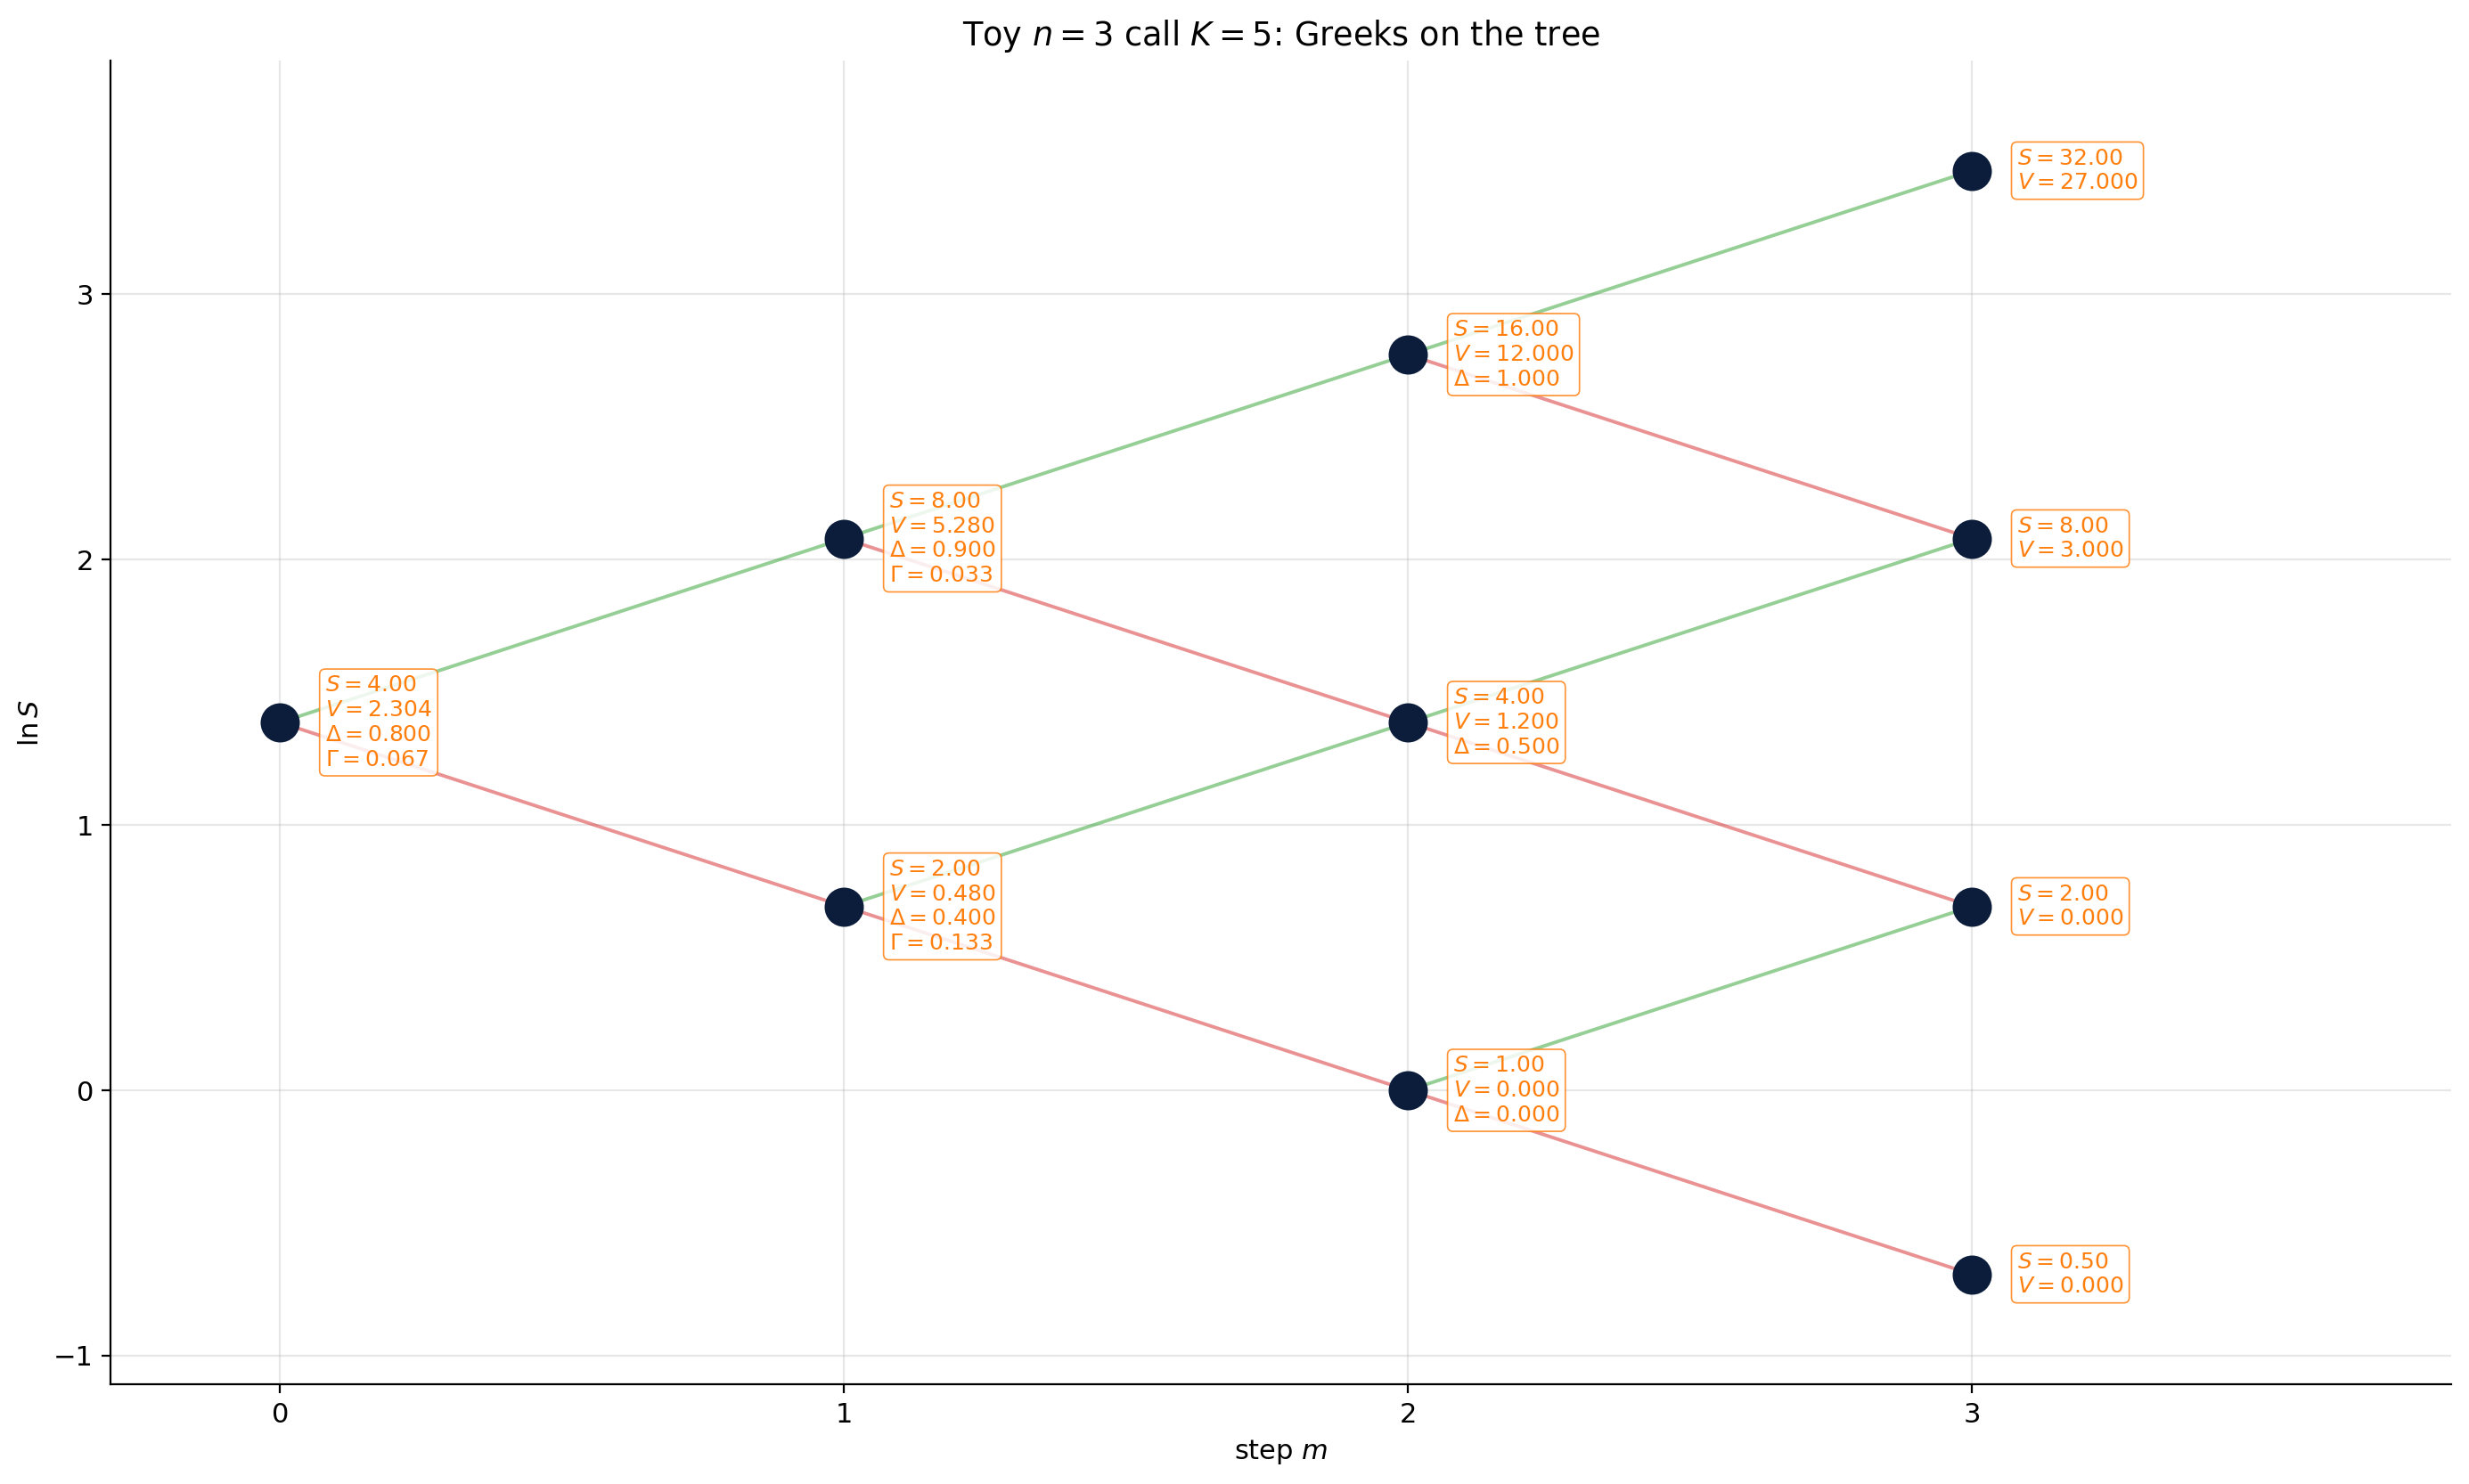
\includegraphics[keepaspectratio]{figures/ch02-greeks-tree.png}}
\caption{ST \(n=3\) call: every node carries \((V, \Delta, \Gamma)\) ---
full Greek board on a lattice.}
\end{figure}

\begin{figure}
\centering
\pandocbounded{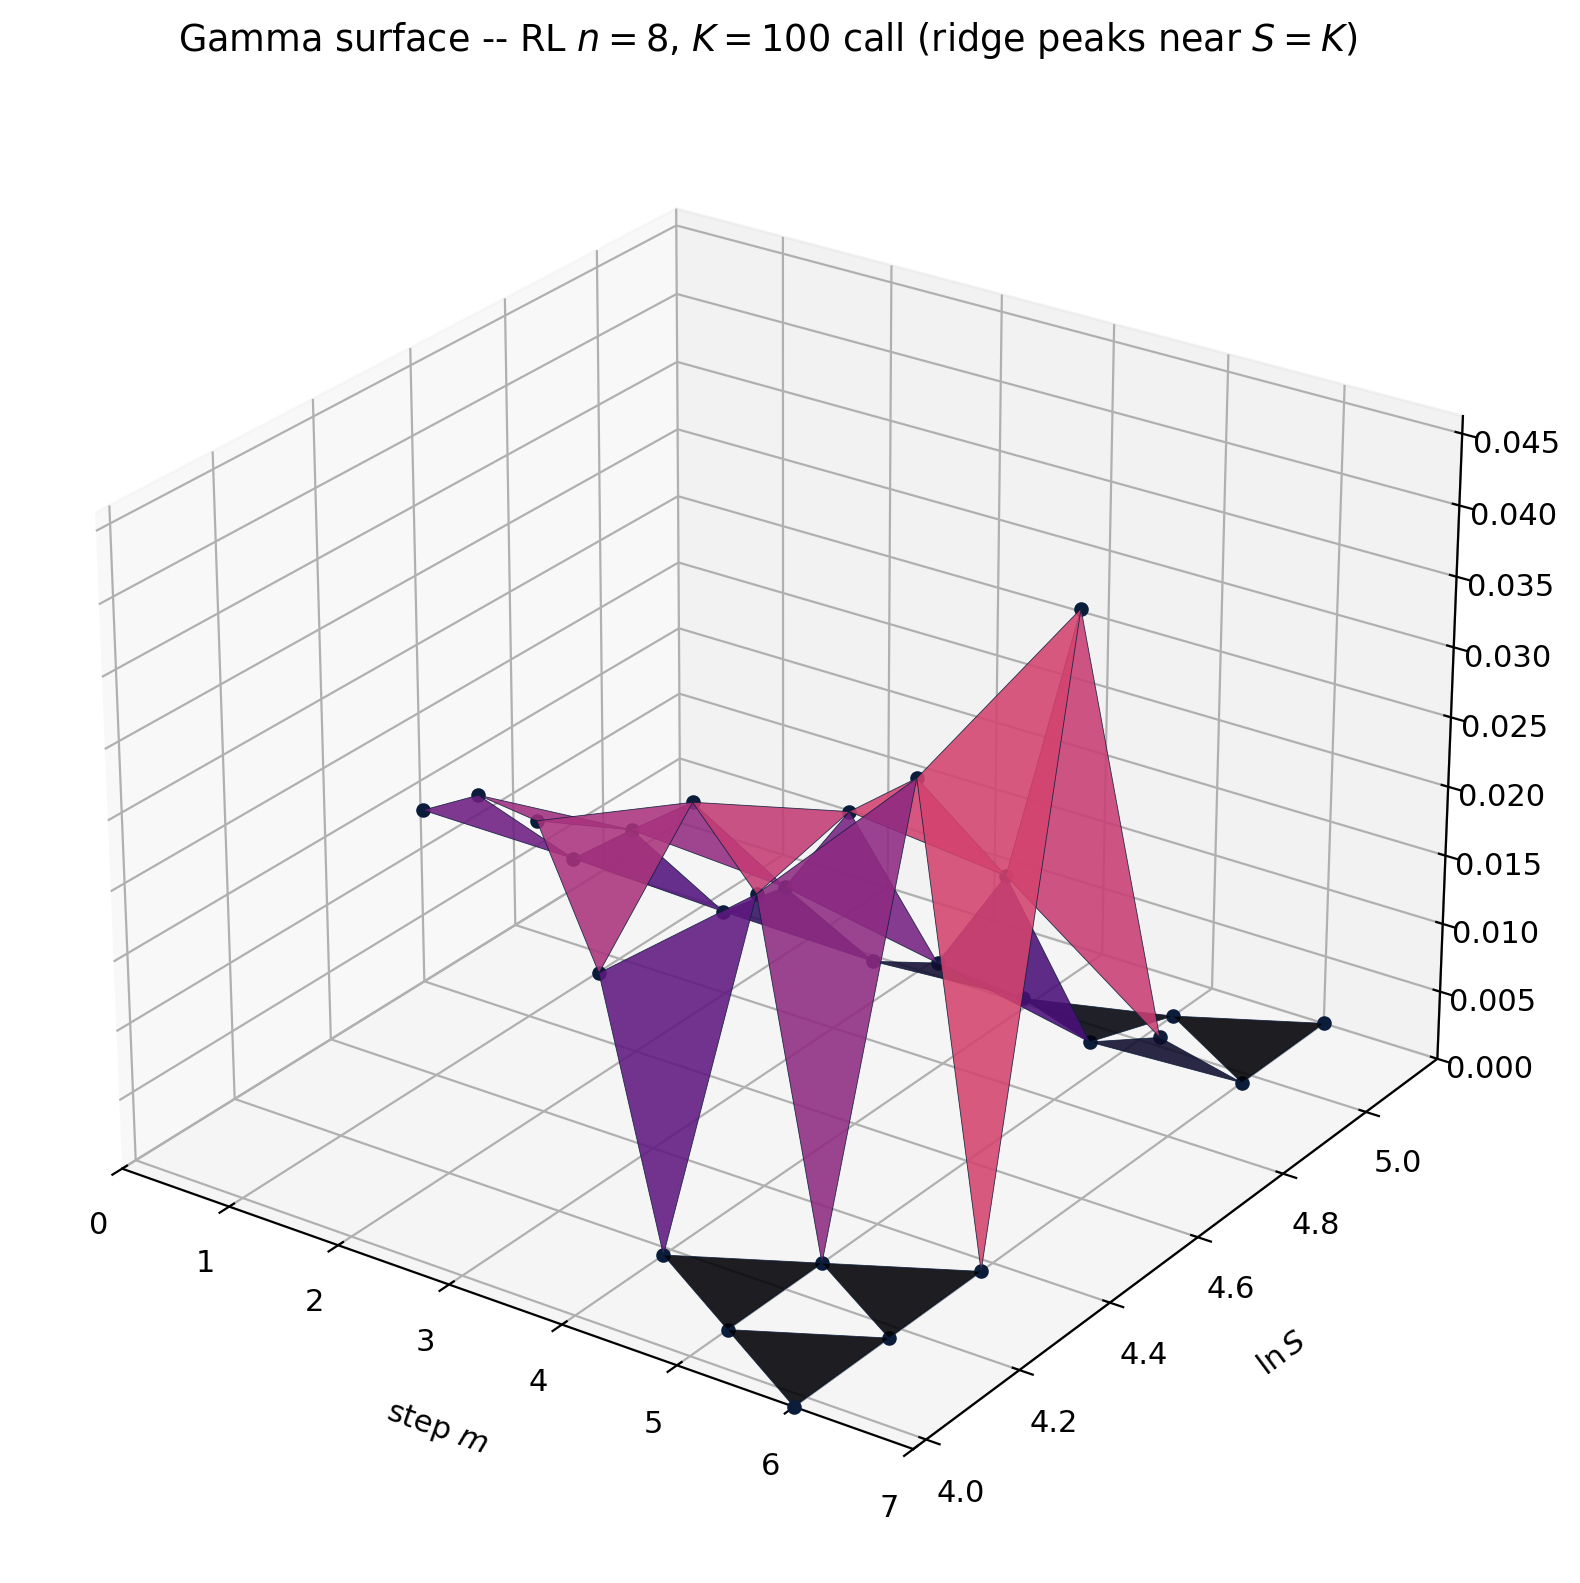
\includegraphics[keepaspectratio]{figures/ch02-gamma-surface.png}}
\caption{Gamma surface on the RL \(n=8\) call lattice. The pointy ridge
sits near \(S=K=100\), exactly where the BS gamma peaks.}
\end{figure}

\begin{figure}
\centering
\pandocbounded{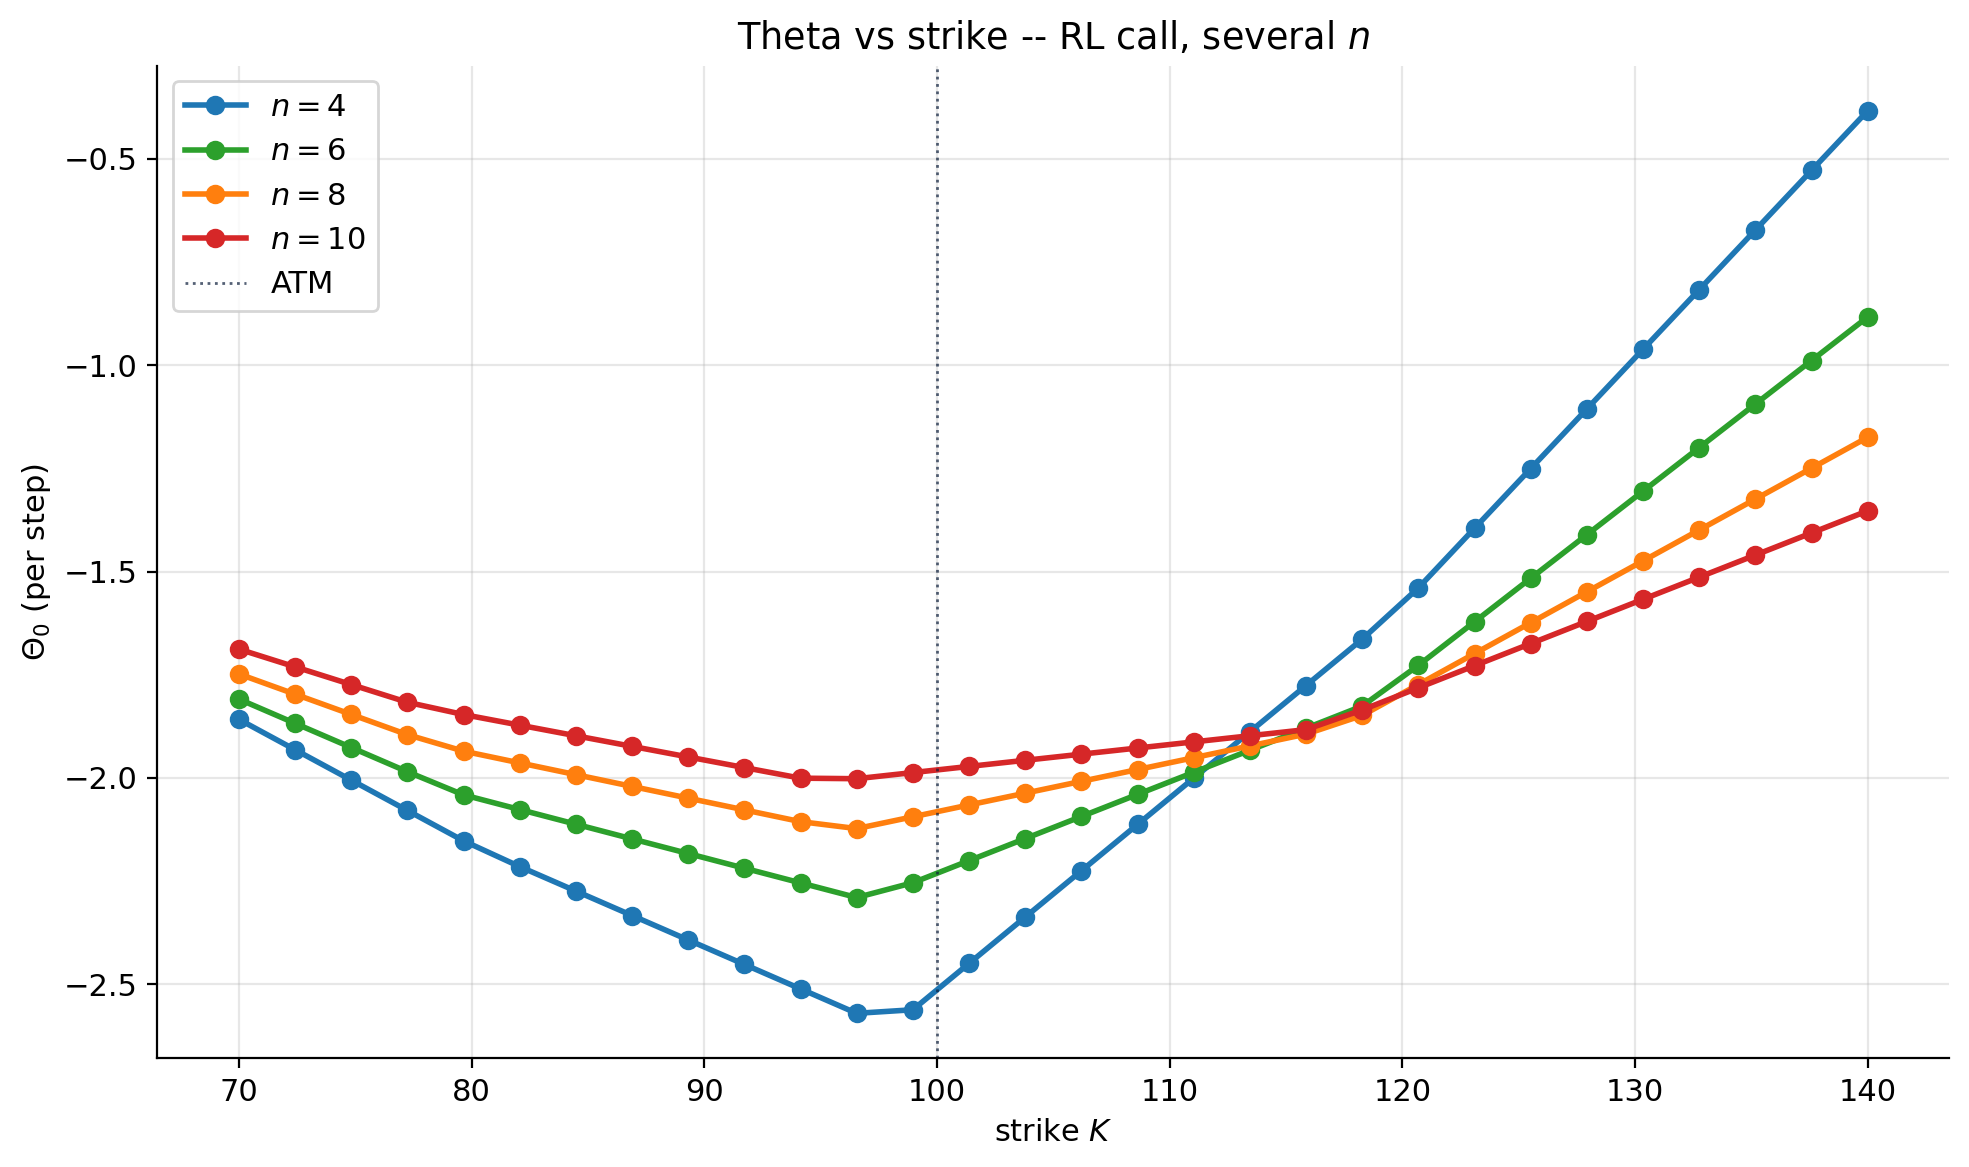
\includegraphics[keepaspectratio]{figures/ch02-theta-lines.png}}
\caption{Theta vs strike on the RL call tree for several \(n\). ATM
theta is most negative (max time decay), wings flatten.}
\end{figure}

\subsection{\texorpdfstring{Example 2.7.1 --- ST \(n=2\) call Greeks at
root}{Example 2.7.1 --- ST n=2 call Greeks at root}}\label{example-2.7.1-st-n2-call-greeks-at-root}

From Example 2.2.1: \(V_{1,1}=4.4\), \(V_{1,0}=0\). \[
\Delta_0 = \frac{4.4-0}{8-2}=0.7333.
\]

Level-1 deltas: -
\(\Delta_{1,1}=(V_{2,2}-V_{2,1})/(S_{2,2}-S_{2,1})=(11-0)/(16-4)=0.9167\).
- \(\Delta_{1,0}=(V_{2,1}-V_{2,0})/(S_{2,1}-S_{2,0})=(0-0)/(4-1)=0\).

\[
\Gamma_0 = \frac{0.9167-0}{0.5\cdot(16-1)} = \frac{0.9167}{7.5}=0.1222.
\]

Theta: \(V_{2,1}=0\) (after one up + one down, \(S\) back to 4),
\(V_0=1.76\). \[
\Theta_0 = \frac{0-1.76}{2} = -0.88.
\]

\subsection{\texorpdfstring{Example 2.7.2 --- RL \(n=4\) call \(K=100\)
Greeks at
root}{Example 2.7.2 --- RL n=4 call K=100 Greeks at root}}\label{example-2.7.2-rl-n4-call-k100-greeks-at-root}

Reading \(V\) off the full rollback (every node, \(\tilde p=0.6\),
discount \(1/1.02\)): - Terminal \(m=4\): payoffs
\((0,0,0,19.79,46.41)\). - \(m=3\):
\(V_{3,3}=(0.6\cdot 46.41+0.4\cdot 19.79)/1.02=35.061\);
\(V_{3,2}=(0.6\cdot 19.79)/1.02=11.641\); \(V_{3,1}=V_{3,0}=0\). -
\(m=2\): \(V_{2,2}=(0.6\cdot 35.061+0.4\cdot 11.641)/1.02=25.189\);
\(V_{2,1}=(0.6\cdot 11.641)/1.02=6.848\); \(V_{2,0}=0\). - \(m=1\):
\(V_{1,1}=(0.6\cdot 25.189+0.4\cdot 6.848)/1.02=17.503\);
\(V_{1,0}=(0.6\cdot 6.848)/1.02=4.028\). - \(m=0\):
\(V_0=(0.6\cdot 17.503+0.4\cdot 4.028)/1.02=11.875\). ✓

With \(S_{1,1}=110\), \(S_{1,0}=90\): \[
\Delta_0 \;=\; (17.503-4.028)/20 \;=\; 0.6738.
\]

Level-1 deltas: -
\(\Delta_{1,1} = (V_{2,2}-V_{2,1})/(S_{2,2}-S_{2,1}) = (25.189-6.848)/(121-99) = 0.8337\).
-
\(\Delta_{1,0} = (V_{2,1}-V_{2,0})/(S_{2,1}-S_{2,0}) = (6.848-0)/(99-81) = 0.3804\).

\[
\Gamma_0 \;=\; (0.8337-0.3804)/(0.5\cdot(121-81)) \;=\; 0.4533/20 \;=\; 0.02266.
\]

Theta: \[
\Theta_0 \;=\; (V_{2,1}-V_0)/2 \;=\; (6.848-11.875)/2 \;=\; -2.514.
\]

\subsection{Example 2.7.3 --- Put delta = call delta −
1}\label{example-2.7.3-put-delta-call-delta-1}

By parity, \(C - P = S_0 - K(1+r)^{-n}\), so
\(\Delta^C - \Delta^P = 1\), hence \(\Delta^P = \Delta^C - 1\). For RL:
\(\Delta^P_0 \approx 0.6738 - 1 = -0.3262\).

\subsection{Example 2.7.4 --- Call gamma = put
gamma}\label{example-2.7.4-call-gamma-put-gamma}

Parity \(C-P=S_0-K(1+r)^{-n}\) is linear in \(S\), so the
second-difference operator on the lattice annihilates it:
\(\Gamma^C - \Gamma^P = 0\), i.e.~\(\Gamma^C = \Gamma^P\) node by node.
Numerically on the RL tree, both come out to \(0.02266\).

\subsection{Example 2.7.5 --- Hedge slippage from a stale
delta}\label{example-2.7.5-hedge-slippage-from-a-stale-delta}

If the dealer sets \(\Delta_0=0.6738\) at \(t=0\) and \textbf{does not
rebalance} for two steps, what happens? The root cash bond is
\(B_0 = V_0 - \Delta_0 S_0 = 11.875 - 0.6738\cdot 100 = -55.505\)
(borrow \(55.505\)).

Stale portfolio value at \(m=2\), by node:

{\def\LTcaptype{none} % do not increment counter
\begin{table}[H]
\centering
\begin{tabular}{|l|r|r|r|r|}
\toprule
outcome & \(S_2\) & stale \(=\Delta_0 S_2+B_0(1+r)^2\) & true \(V_{2,k}\) & gap (stale − true) \\
\midrule



UU & \(121\) & \(0.6738\cdot 121-55.505\cdot 1.0404=23.78\) & \(25.189\)
& \(-1.41\) \\
UD & \(\phantom{0}99\) &
\(0.6738\cdot \phantom{0}99-55.505\cdot 1.0404=\phantom{0}8.96\) &
\(\phantom{0}6.848\) & \(+2.11\) \\
DD & \(\phantom{0}81\) &
\(0.6738\cdot \phantom{0}81-55.505\cdot 1.0404=-3.17\) &
\(\phantom{0}0.000\) & \(-3.17\) \\
\bottomrule
\end{tabular}
\end{table}
}

The RN-weighted gap is
\(\tilde p^2(-1.41)+2\tilde p(1-\tilde p)(+2.11)+(1-\tilde p)^2(-3.17) = 0.36\cdot(-1.41)+0.48\cdot 2.11+0.16\cdot(-3.17) = -0.508+1.013-0.507 = -0.002 \approx 0\)
--- the stale portfolio is fair on average (no arbitrage), but the
\textbf{per-path} deviations from \(V_{2,k}\) are exactly the gamma cost
the dealer eats by not rebalancing. The magnitudes scale with
\(\tfrac12\Gamma_0\cdot(\Delta S)^2\) and the convexity of the payoff.
Chapter 9 generalises.

\subsection{Example 2.7.6 --- Vega is not a tree
Greek}\label{example-2.7.6-vega-is-not-a-tree-greek}

We never bumped \(u\) or \(d\). Vega = \(\partial V/\partial \sigma\)
requires re-tagging \(u(\sigma), d(\sigma)\) and bumping. Chapter 7 sets
that up via \(u=e^{\sigma\sqrt{\Delta t}}\).

\subsection{Example 2.7.7 --- Sign of theta for a long
call}\label{example-2.7.7-sign-of-theta-for-a-long-call}

\(\Theta_0<0\) in both ST and RL: time decay is bad for a long option.
As expiry approaches, \(V\) slides down toward intrinsic value
\((S-K)^+\).

\subsection{\texorpdfstring{Table 2.7.1 --- ST \(n=3\) call Greek board
(\(K=5\))}{Table 2.7.1 --- ST n=3 call Greek board (K=5)}}\label{table-2.7.1-st-n3-call-greek-board-k5}

{\def\LTcaptype{none} % do not increment counter
\begin{table}[H]
\centering
\begin{tabular}{|l|r|r|r|r|}
\toprule
\((m,k)\) & \(S\) & \(V\) & \(\Delta\) & \(\Gamma\) \\
\midrule



\((0,0)\) & \(\phantom{0}4\) & \(\phantom{0}2.304\) & \(0.800\) &
\(0.0667\) \\
\((1,0)\) & \(\phantom{0}2\) & \(\phantom{0}0.480\) & \(0.400\) &
\(0.1333\) \\
\((1,1)\) & \(\phantom{0}8\) & \(\phantom{0}5.280\) & \(0.900\) &
\(0.0333\) \\
\((2,0)\) & \(\phantom{0}1\) & \(\phantom{0}0.000\) & \(0.000\) & \\
\((2,1)\) & \(\phantom{0}4\) & \(\phantom{0}1.200\) & \(0.500\) & \\
\((2,2)\) & \(16\) & \(12.000\) & \(1.000\) & \\
\bottomrule
\end{tabular}
\end{table}
}

\emph{Blank: \(\Gamma\) not defined at terminal nodes (no children to
take a second difference against).}

Row computations (Delta from forward children; Gamma from child-Delta
difference scaled by half the grand-child spot span): -
\(\Delta_{0,0}=(5.280-0.480)/(8-2)=0.800\);
\(\Gamma_{0,0}=(0.900-0.400)/(\tfrac12(16-1))=0.500/7.5=0.0667\). -
\(\Delta_{1,0}=(1.200-0)/(4-1)=0.400\);
\(\Gamma_{1,0}=(0.500-0)/(\tfrac12(8-0.5))=0.500/3.75=0.1333\). -
\(\Delta_{1,1}=(12-1.2)/(16-4)=0.900\);
\(\Gamma_{1,1}=(1.000-0.500)/(\tfrac12(32-2))=0.500/15=0.0333\). -
\(\Delta_{2,0}=(0-0)/(2-0.5)=0\); \(\Delta_{2,1}=(3-0)/(8-2)=0.500\);
\(\Delta_{2,2}=(27-3)/(32-8)=1.000\).

\subsection{\texorpdfstring{Table 2.7.2 --- RL \(n=4\) call Greek board
(root + first
layer)}{Table 2.7.2 --- RL n=4 call Greek board (root + first layer)}}\label{table-2.7.2-rl-n4-call-greek-board-root-first-layer}

{\def\LTcaptype{none} % do not increment counter
\begin{table}[H]
\centering
\begin{tabular}{|l|r|r|r|r|}
\toprule
\((m,k)\) & \(S\) & \(V\) & \(\Delta\) & \(\Gamma\) \\
\midrule



\((0,0)\) & \(100.0\) & \(11.875\) & \(0.6738\) & \(0.02266\) \\
\((1,0)\) & \(\phantom{0}90.0\) & \(\phantom{00}4.028\) & \(0.3804\) &
\(0.03266\) \\
\((1,1)\) & \(110.0\) & \(17.503\) & \(0.8337\) & \(0.01727\) \\
\bottomrule
\end{tabular}
\end{table}
}

\begin{figure}
\centering
\pandocbounded{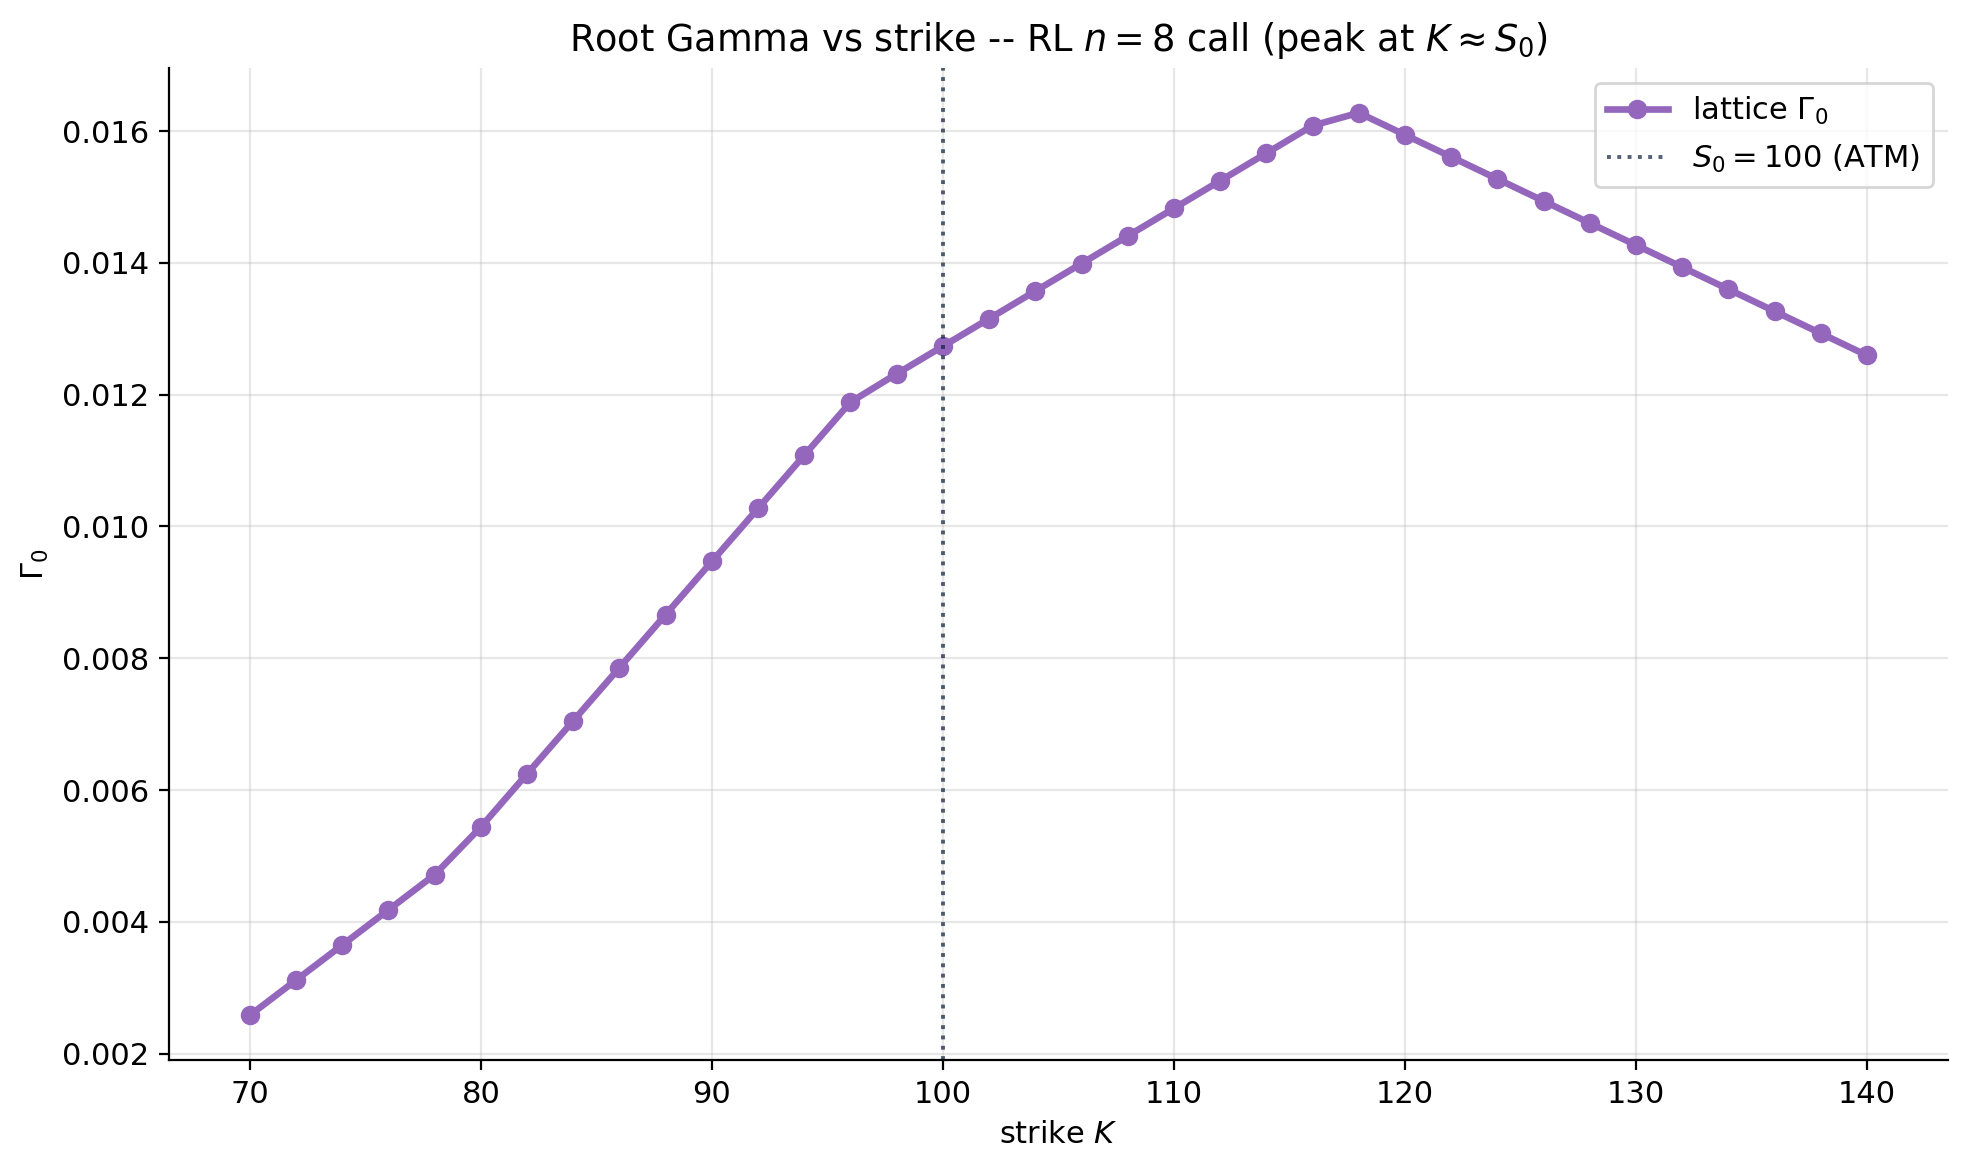
\includegraphics[keepaspectratio]{figures/ch02-gamma-vs-S.png}}
\caption{Lattice Gamma at the root as a function of strike \(K\), on the
RL \(n=8\) recombining tree. The bell peaks at the money --- the classic
Gamma profile, computed entirely from finite differences with no
calculus.}
\end{figure}

\subsection{Exercises 2.7}\label{exercises-2.7}

\textbf{Exercise 2.7.A --- Toy-A root Delta from scratch.} On the Toy-A
tree (ST: \(S_0=4, u=2, d=1/2, r=1/4\), \(\tilde p=1/2\)), price a
\(K=5\) European call at \(n=2\) and compute \(\Delta_0\) from the
finite-difference formula.

\begin{quote}
\textbf{Answer.} Terminal payoffs at \(n=2\):
\((S_{2,0}, S_{2,1}, S_{2,2})=(1,4,16)\Rightarrow (V_{2,0},V_{2,1},V_{2,2})=(0,0,11)\).
Roll back: \(V_{1,1}=(0.5\cdot 11+0.5\cdot 0)/1.25=4.4\), \(V_{1,0}=0\).
Then \(\Delta_0=(4.4-0)/(8-2)=\mathbf{0.7333}\). Matches Example 2.7.1.
\end{quote}

\textbf{Exercise 2.7.B --- Realistic Gamma at an up-node.} On the RL
tree (\(S_0=100, u=1.10, d=0.90, r=0.02, \tilde p=0.6\)), compute
\(\Gamma_{1,1}\) for the \(K=100\), \(n=4\) call. (You may use the
rollback values from Example 2.7.2: \(V_{2,2}=25.189\),
\(V_{2,1}=6.848\), \(V_{3,3}=35.061\), \(V_{3,2}=11.641\),
\(V_{3,1}=0\).)

\begin{quote}
\textbf{Answer.} Need
\(\Delta_{2,2}=(V_{3,3}-V_{3,2})/(S_{3,3}-S_{3,2})=(35.061-11.641)/(133.10-108.90)=23.420/24.20=0.9678\)
and
\(\Delta_{2,1}=(V_{3,2}-V_{3,1})/(S_{3,2}-S_{3,1})=(11.641-0)/(108.90-89.10)=11.641/19.80=0.5879\).
Spot spread at level 3 across grandchildren of \((1,1)\):
\(S_{3,3}-S_{3,1}=133.10-89.10=44.0\). So
\(\Gamma_{1,1}=(0.9678-0.5879)/(0.5\cdot 44.0)=0.3799/22.0=\mathbf{0.01727}\).
Smaller than \(\Gamma_0=0.02266\) --- Gamma is decaying as we move ITM.
\end{quote}

\textbf{Exercise 2.7.C --- Sign rules.} For each of (i) long call, (ii)
long put, (iii) short straddle, state the sign of \(\Delta_0\),
\(\Gamma_0\), \(\Theta_0\) on the RL tree, and explain in one line.

\begin{quote}
\textbf{Answer.} (i) Long call: \(\Delta_0>0\) (up moves help),
\(\Gamma_0>0\) (convex payoff), \(\Theta_0<0\) (time decay hurts the
long). (ii) Long put: \(\Delta_0<0\), \(\Gamma_0>0\) (still convex),
\(\Theta_0<0\). (iii) Short straddle = \(-C-P\): \(\Delta_0\approx 0\)
(parity gives \(\Delta_C+\Delta_P=2\Delta_C-1\); at ATM both deltas
roughly cancel to \(0\)), \(\Gamma_0<0\) (short the convexity),
\(\Theta_0>0\) (time decay accrues to the short). The Greeks of a
portfolio are sums of the per-leg Greeks --- no new theory needed.
\end{quote}

\begin{center}\rule{0.5\linewidth}{0.5pt}\end{center}

\section{\texorpdfstring{2.8 Convergence and the role of \(n\) ---
preview of Chapter
7}{2.8 Convergence and the role of n --- preview of Chapter 7}}\label{convergence-and-the-role-of-n-preview-of-chapter-7}

\begin{quote}
\textbf{Punchline.} Choose \(u=e^{\sigma\sqrt{T/n}}\), \(d=1/u\),
\(r_n=rT/n\). Then as \(n\to\infty\), the CRR call price
\textbf{converges to Black--Scholes}, at a rate roughly \(1/n\). The
whole continuous-time machinery is the \textbf{limit} of this lattice.
\end{quote}

The full proof is Chapter 7. Here we just look at the numerics.

\begin{figure}
\centering
\pandocbounded{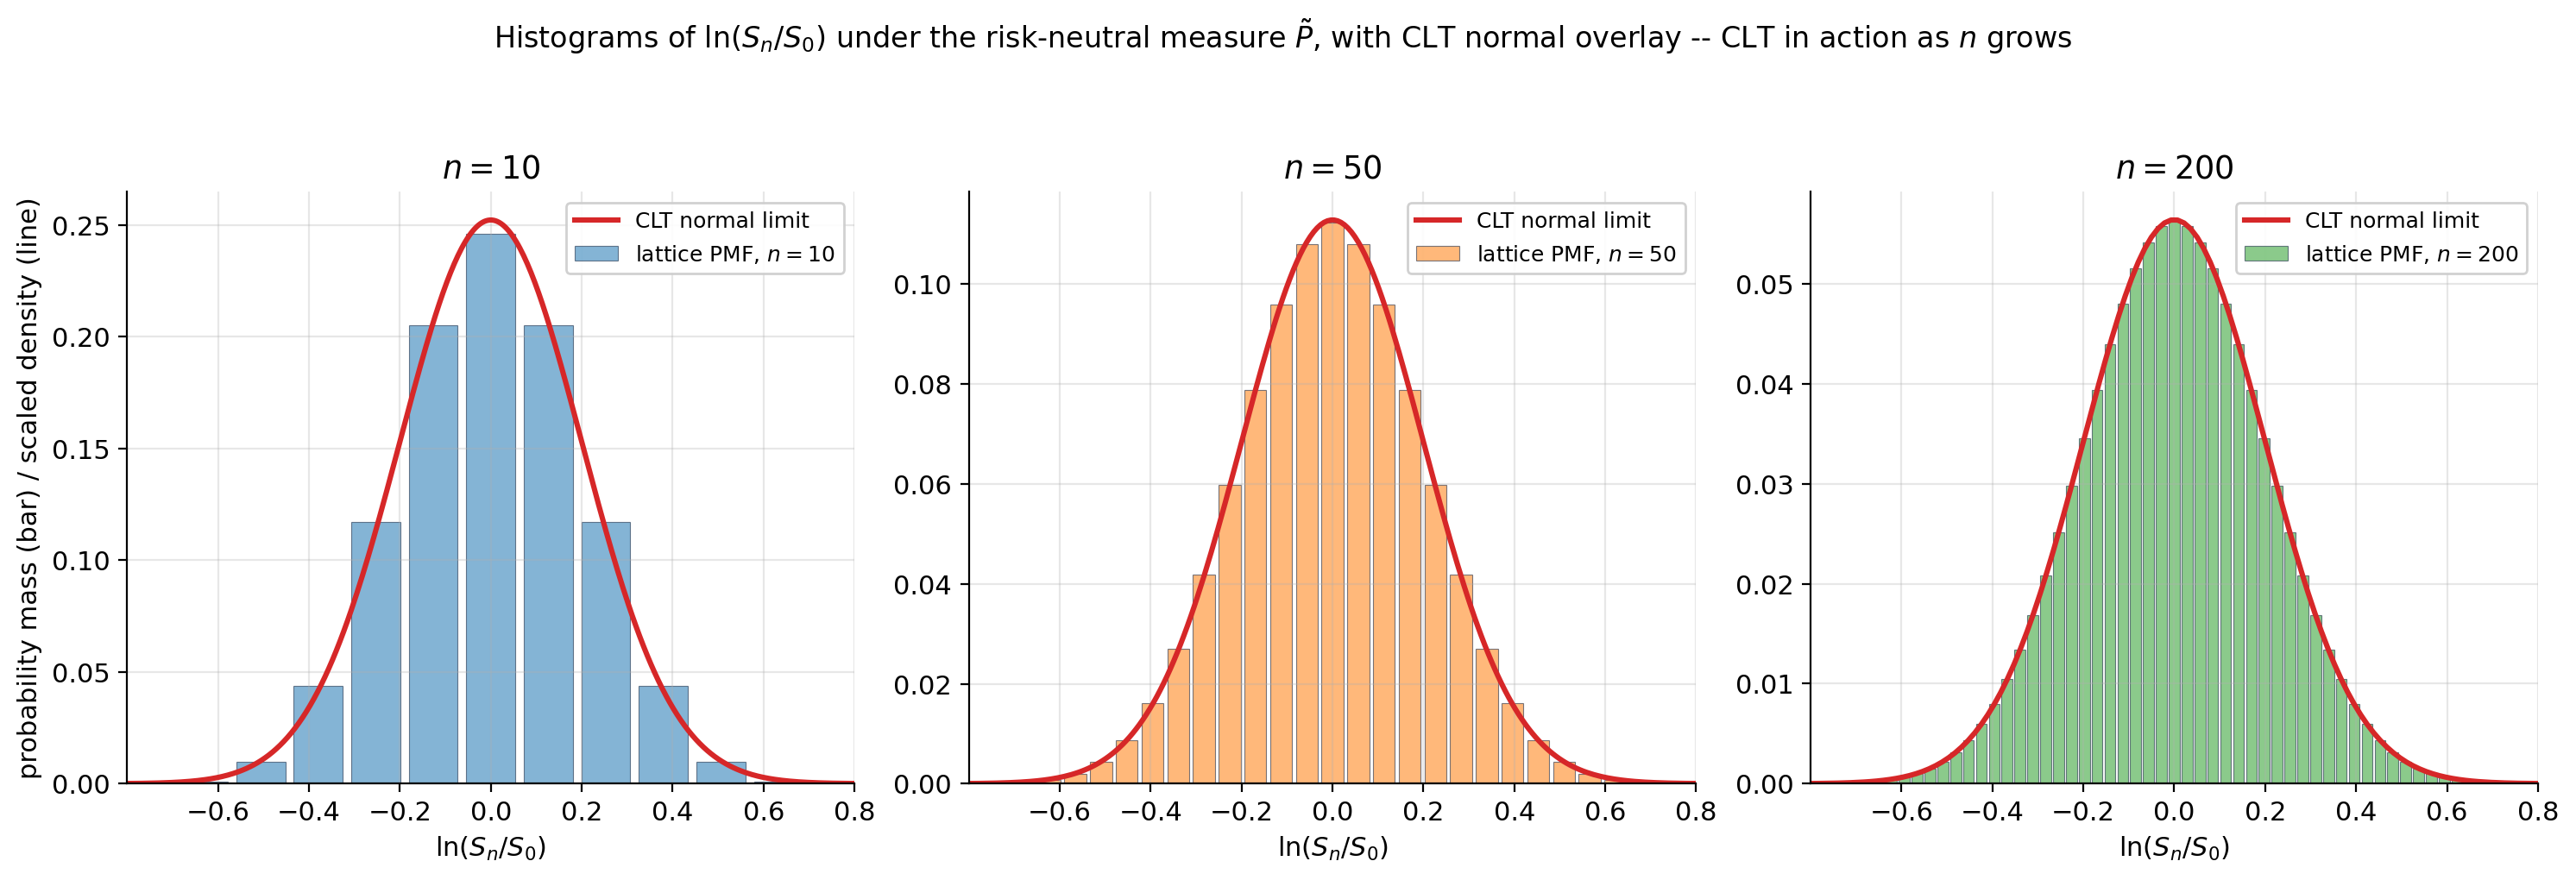
\includegraphics[keepaspectratio]{figures/ch02-logS-overlay.png}}
\caption{Histograms of \(\ln S_n\) under \(\tilde{\mathbb P}\) for
\(n=10,50,200\), overlaid with the normal limit. The CLT in action.}
\end{figure}

\begin{figure}
\centering
\pandocbounded{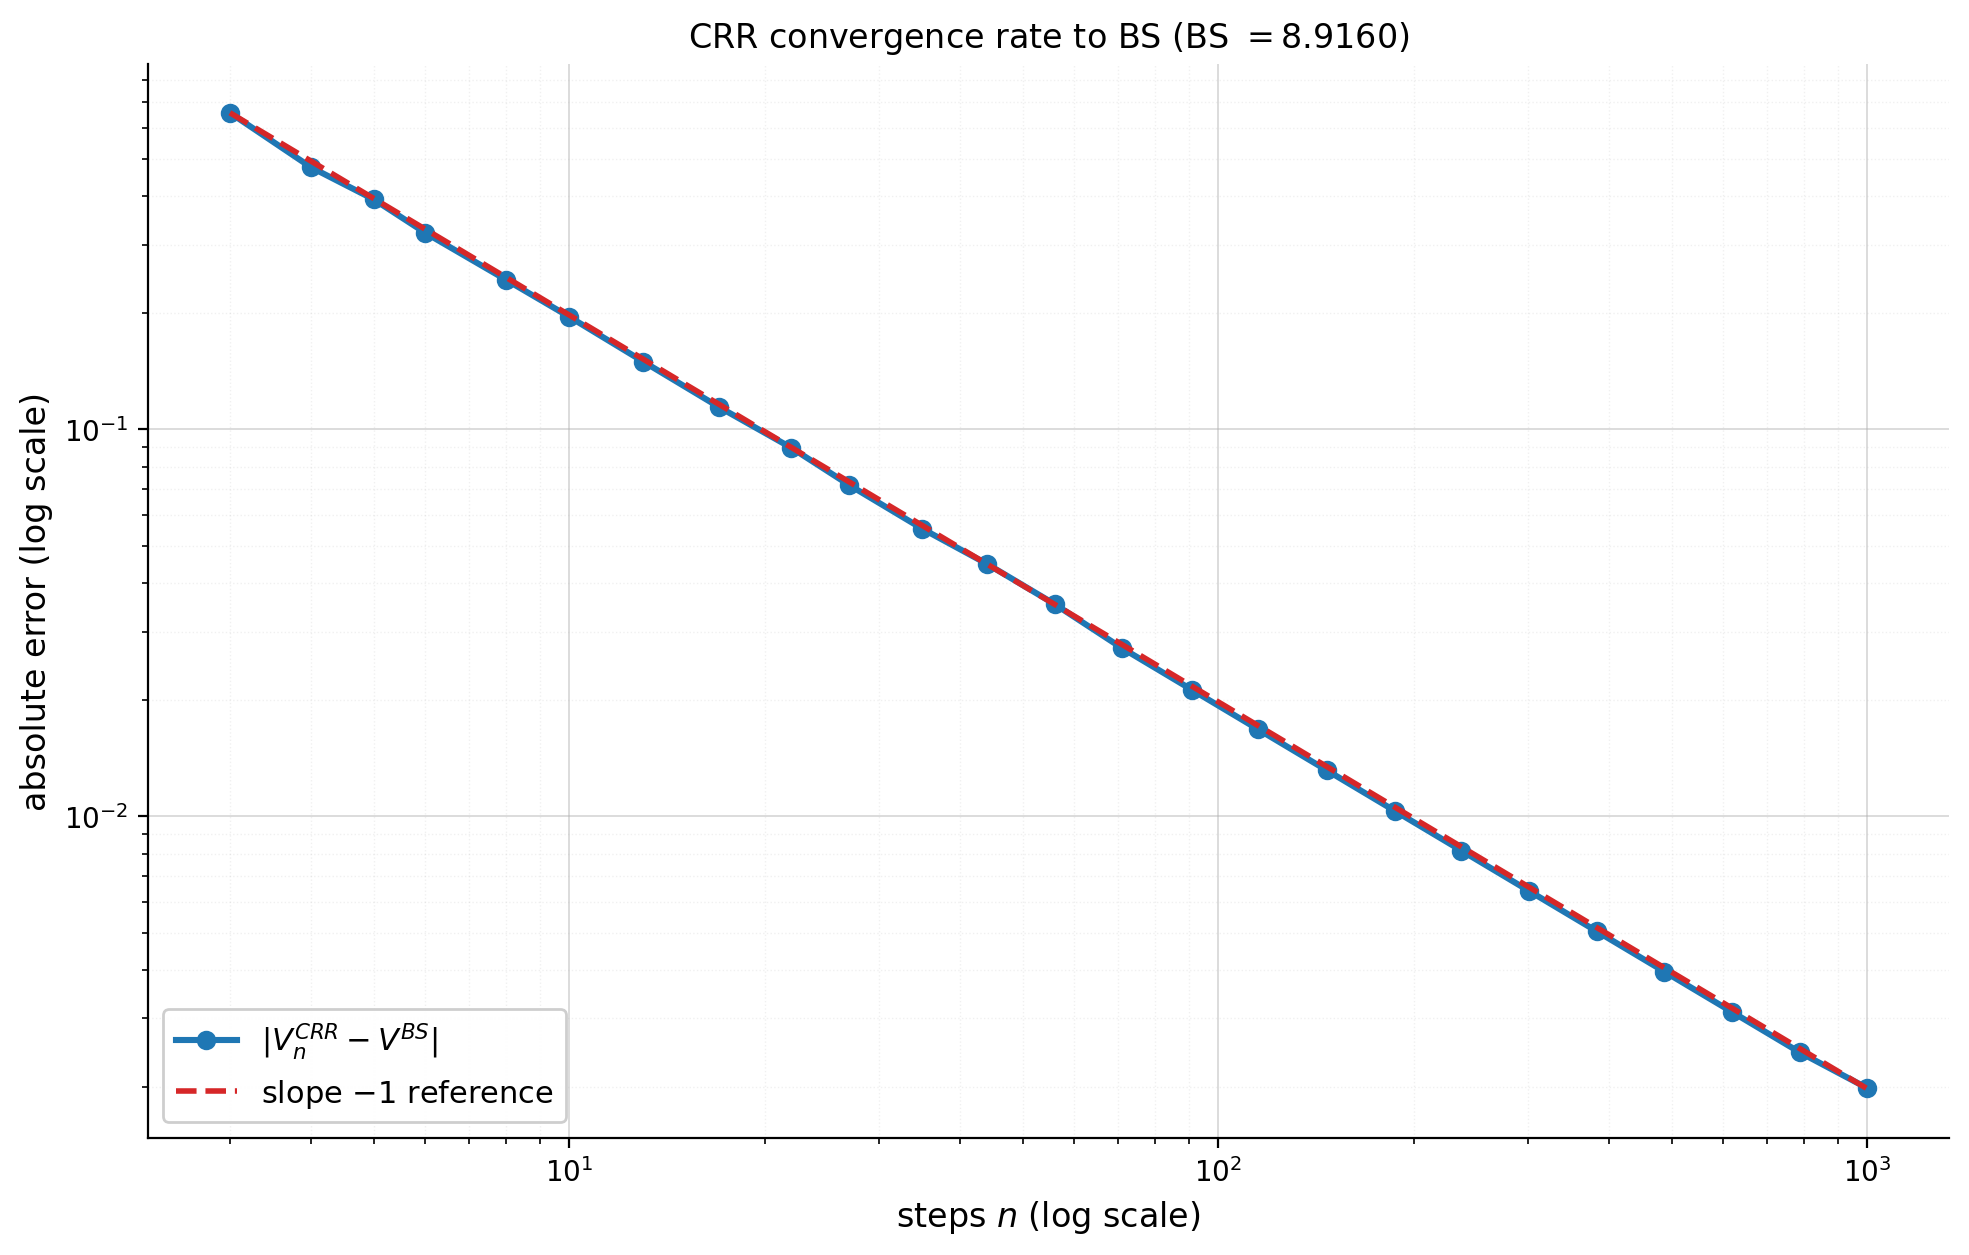
\includegraphics[keepaspectratio]{figures/ch02-error-loglog.png}}
\caption{Log--log plot of \(|V_n^{CRR}-V^{BS}|\) vs \(n\). Slope
\(\approx -1\).}
\end{figure}

\subsection{\texorpdfstring{Example 2.8.1 --- RL call \(S_0=K=100\),
\(r=2\%\), \(\sigma=20\%\),
\(T=1\)}{Example 2.8.1 --- RL call S\_0=K=100, r=2\textbackslash\%, \textbackslash sigma=20\textbackslash\%, T=1}}\label{example-2.8.1-rl-call-s_0k100-r2-sigma20-t1}

The Black--Scholes price is

\[
V^{BS} \;=\; S_0\Phi(d_1) - Ke^{-rT}\Phi(d_2) \;\approx\; 8.916.
\]

CRR prices at \(\sigma\)-matched \(u,d\):

{\def\LTcaptype{none} % do not increment counter
\begin{table}[H]
\centering
\begin{tabular}{|r|r|r|}
\toprule
\(n\) & \(V_0^{CRR}\) & \(\lvert V_0^{CRR}-V^{BS}\rvert\) \\
\midrule



\(\phantom{000}1\) & \(9.504\) & \(0.5880\) \\
\(\phantom{000}2\) & \(9.087\) & \(0.1710\) \\
\(\phantom{000}4\) & \(8.957\) & \(0.0410\) \\
\(\phantom{000}8\) & \(8.945\) & \(0.0290\) \\
\(\phantom{00}20\) & \(8.927\) & \(0.0110\) \\
\(\phantom{00}50\) & \(8.921\) & \(0.0050\) \\
\(\phantom{0}200\) & \(8.917\) & \(0.0010\) \\
\(1000\) & \(8.916\) & \(0.0003\) \\
\bottomrule
\end{tabular}
\end{table}
}

The error halves roughly when \(n\) doubles --- slope \(-1\) on log--log
axes.

\subsection{Example 2.8.2 --- Put convergence via
parity}\label{example-2.8.2-put-convergence-via-parity}

Each \(V^P_n = V^C_n - S_0 + Ke^{-rT}\), with \textbf{parity holding
exactly at every \(n\)}. So the put error tracks the call error.

\subsection{\texorpdfstring{Example 2.8.3 --- Why
\(u=e^{\sigma\sqrt{\Delta t}}\)?}{Example 2.8.3 --- Why u=e\^{}\{\textbackslash sigma\textbackslash sqrt\{\textbackslash Delta t\}\}?}}\label{example-2.8.3-why-uesigmasqrtdelta-t}

Under \(\tilde{\mathbb P}\), \(\ln(S_n/S_0) = \sum_{i=1}^n X_i\) where
each \(X_i\in\{\ln u,\ln d\}\) with risk-neutral probabilities. Pick
\(u,d,p\) so the mean and variance per step match
\((r-\tfrac12\sigma^2)\Delta t\) and \(\sigma^2\Delta t\). The CRR
choice is one consistent way; the CLT then guarantees \(\ln(S_T/S_0)\)
is asymptotically normal with mean \((r-\tfrac12\sigma^2)T\) and
variance \(\sigma^2 T\), which is the BS log-normal.

\subsection{Example 2.8.4 --- Even-odd
oscillation}\label{example-2.8.4-even-odd-oscillation}

Tree prices typically oscillate up--down--up around BS as \(n\) grows.
Averaging adjacent \(n\)'s (e.g.~Richardson-style \((V_n+V_{n+1})/2\))
doubles the convergence rate. Chapter 7 unpacks this.

\subsection{Example 2.8.5 --- Convergence of
Greeks}\label{example-2.8.5-convergence-of-greeks}

Lattice \(\Delta_0\) and \(\Gamma_0\) converge to BS Greeks at similar
rates. At \(n=200\), RL ATM gamma is within \(\sim 0.5\%\) of BS gamma.

\subsection{Table 2.8.1 --- Convergence
summary}\label{table-2.8.1-convergence-summary}

{\def\LTcaptype{none} % do not increment counter
\begin{table}[H]
\centering
\begin{tabular}{|r|r|r|l|}
\toprule
\(n\) & CRR call \(V_0\) & error & implied trend \\
\midrule



\(\phantom{00}1\) & \(9.504\) & \(0.5880\) & start \\
\(\phantom{00}5\) & \(8.991\) & \(0.0750\) & converging \\
\(\phantom{0}25\) & \(8.928\) & \(0.0120\) & tight \\
\(125\) & \(8.918\) & \(0.0020\) & very tight \\
\(625\) & \(8.916\) & \(0.0005\) & indistinguishable \\
\bottomrule
\end{tabular}
\end{table}
}

\begin{center}\rule{0.5\linewidth}{0.5pt}\end{center}

\section{2.9 Path-independence vs
path-dependence}\label{path-independence-vs-path-dependence}

\begin{quote}
\textbf{Punchline.} The recombining tree only works for payoffs that
depend on \(S_n\) \textbf{alone}. The moment the payoff cares about the
\textbf{path} (Asian average, lookback max, barrier touched), two paths
that recombine to the same leaf become \textbf{different} payoffs ---
and you can no longer collapse them. You either augment the state, or
you simulate.
\end{quote}

A few examples make this concrete.

\begin{figure}
\centering
\pandocbounded{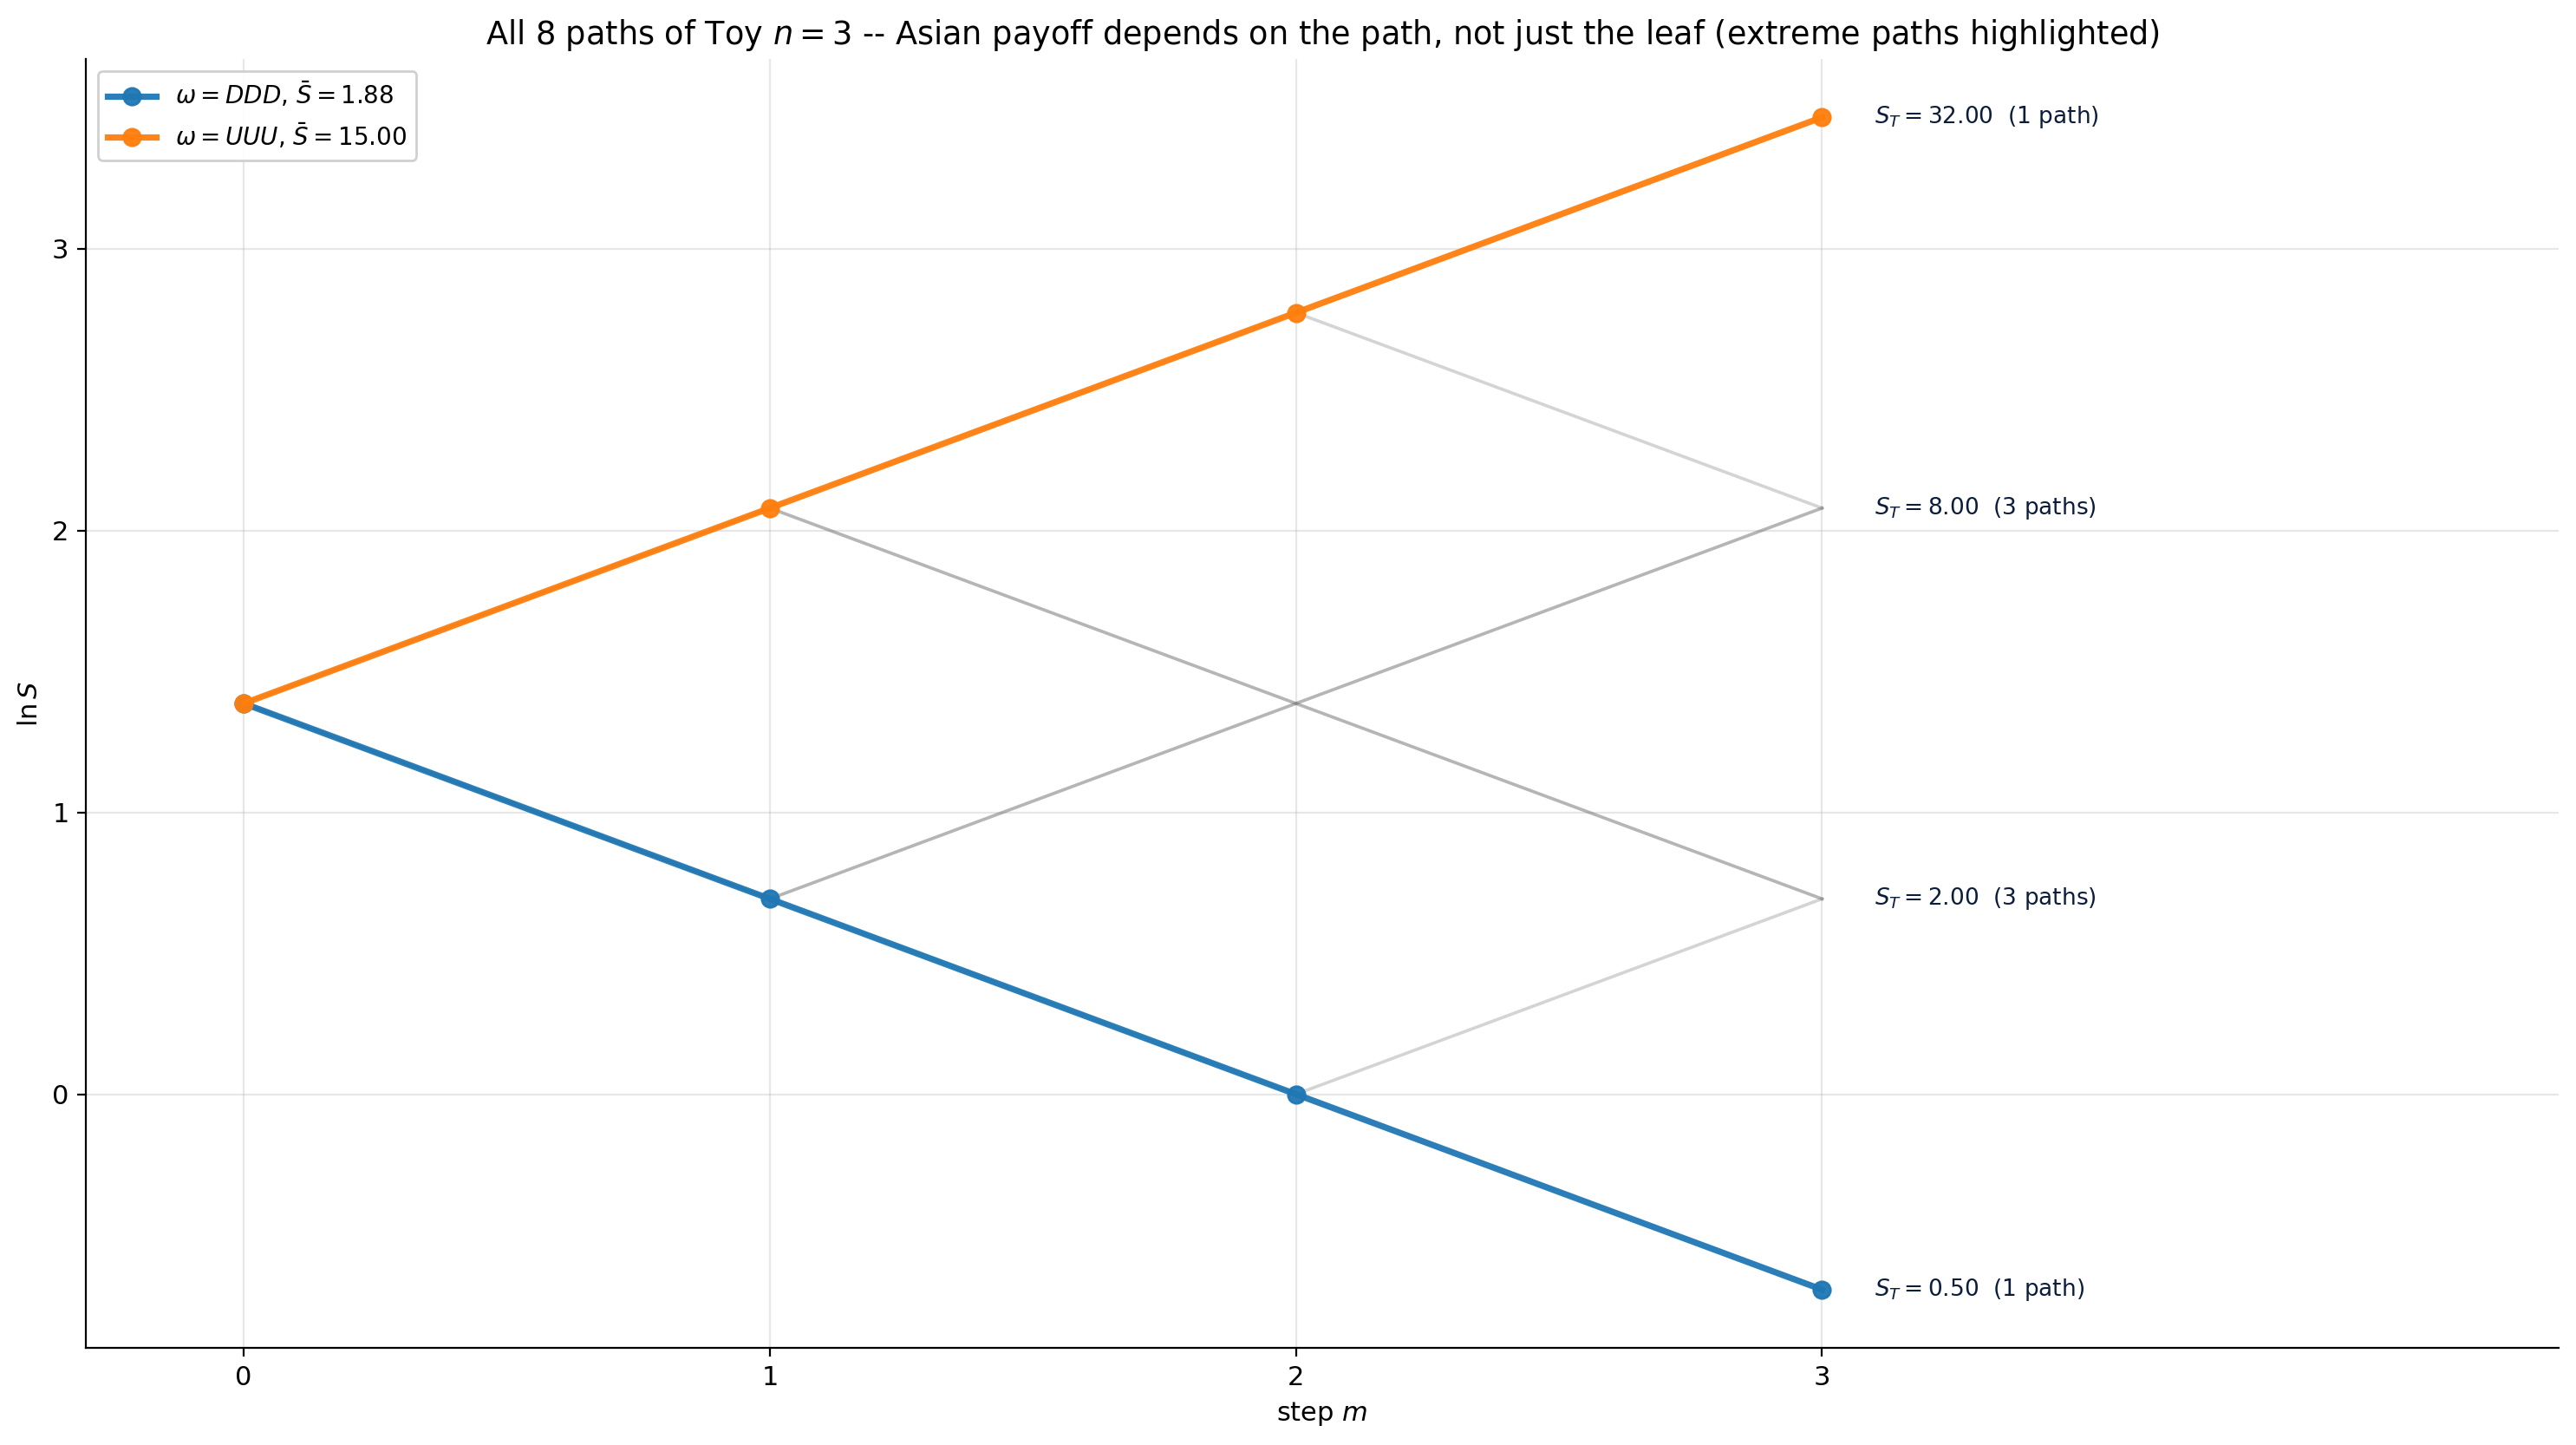
\includegraphics[keepaspectratio]{figures/ch02-bushy-asian.png}}
\caption{All 8 paths of the ST \(n=3\) tree, with each path's average
annotated. Paths UUD, UDU, DUU all end at \(S_3=8\), but their averages
\(\bar S = \frac{1}{4}(S_0+S_1+S_2+S_3)\) are different.}
\end{figure}

\begin{figure}
\centering
\pandocbounded{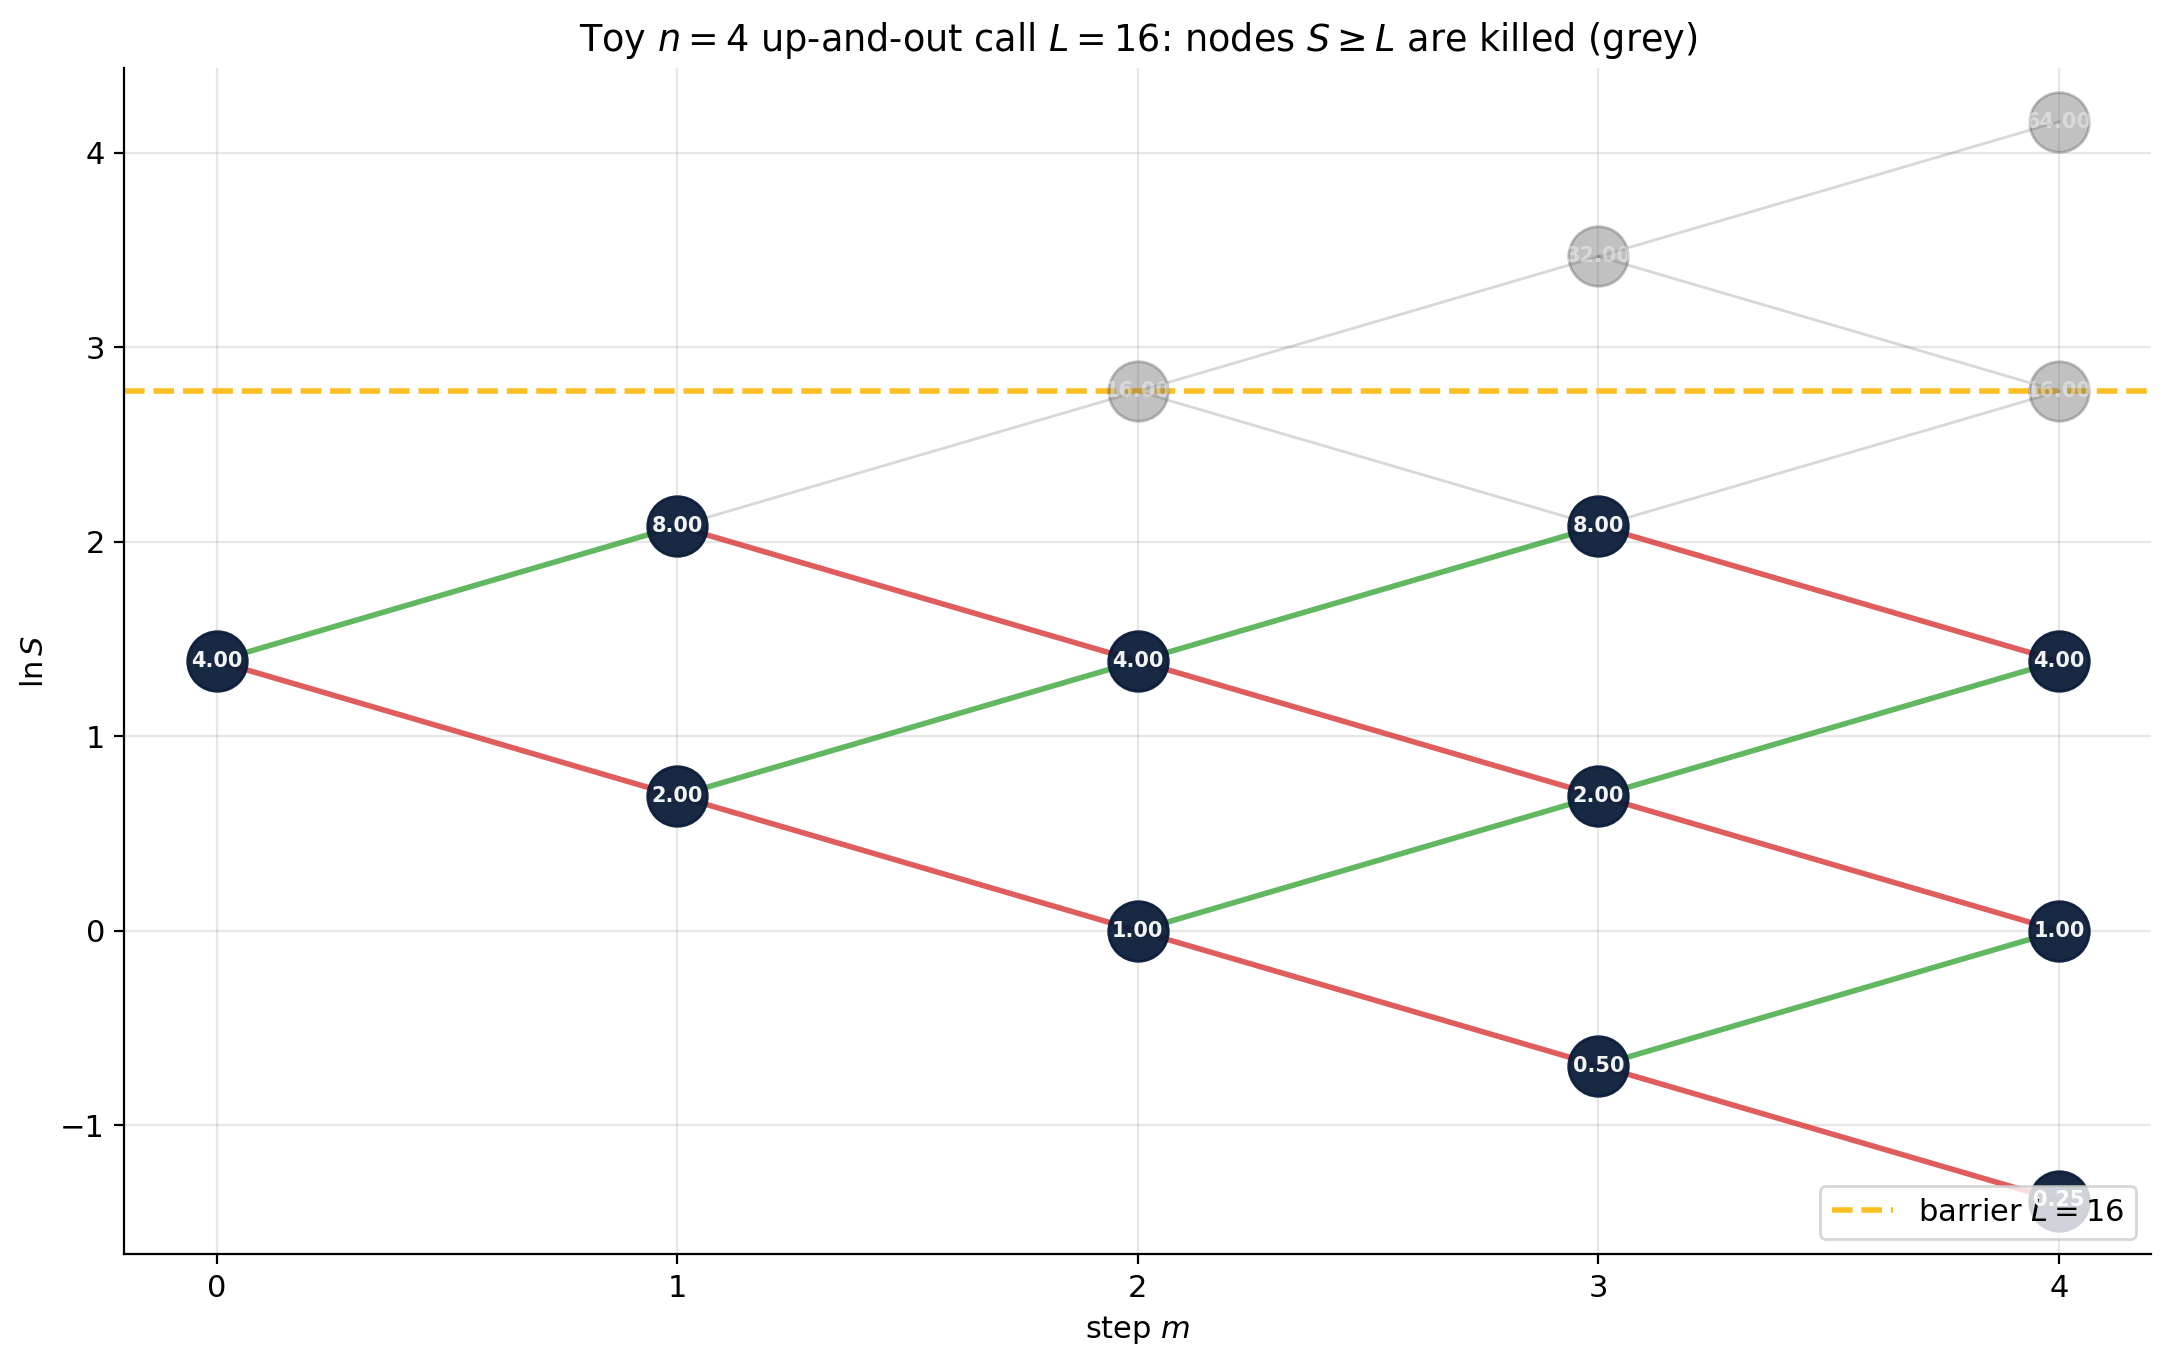
\includegraphics[keepaspectratio]{figures/ch02-knockout-tree.png}}
\caption{Up-and-out barrier \(L=16\) on the ST \(n=4\) lattice. Nodes
that touch or exceed \(L\) are killed (grey).}
\end{figure}

\subsection{\texorpdfstring{Example 2.9.1 --- Asian call on ST \(n=3\),
\(K=5\)}{Example 2.9.1 --- Asian call on ST n=3, K=5}}\label{example-2.9.1-asian-call-on-st-n3-k5}

Asian payoff \((\bar S - K)^+\) with
\(\bar S = \tfrac{1}{4}(S_0+S_1+S_2+S_3)\). The 8 paths split by leaf:

{\def\LTcaptype{none} % do not increment counter
\begin{table}[H]
\centering
\begin{tabular}{|l|l|r|r|}
\toprule
Path & \(S_1,S_2,S_3\) & \(\bar S\) & payoff \\
\midrule



DDD & 2, 1, 0.5 & \(\phantom{0}1.875\) & \(\phantom{0}0.0\) \\
DDU & 2, 1, 2 & \(\phantom{0}2.250\) & \(\phantom{0}0.0\) \\
DUD & 2, 4, 2 & \(\phantom{0}3.000\) & \(\phantom{0}0.0\) \\
DUU & 2, 4, 8 & \(\phantom{0}4.500\) & \(\phantom{0}0.0\) \\
UDD & 8, 4, 2 & \(\phantom{0}4.500\) & \(\phantom{0}0.0\) \\
UDU & 8, 4, 8 & \(\phantom{0}6.000\) & \(\phantom{0}1.0\) \\
UUD & 8, 16, 8 & \(\phantom{0}9.000\) & \(\phantom{0}4.0\) \\
UUU & 8, 16, 32 & \(15.000\) & \(10.0\) \\
\bottomrule
\end{tabular}
\end{table}
}

Notice DUU and UDD both end at \(S_3=8\) but have \textbf{different
averages}. The recombining tree's claim ``the value depends only on
\((m,k)\)'' is \textbf{false} for the Asian.

RN price under \(\tilde p=0.5\) (each path has weight \(1/8\)): \[
V_0^{\text{Asian}} \;=\; \frac{1}{(1.25)^3}\cdot\frac{1}{8}\bigl[0+0+0+0+0+1+4+10\bigr]
\;=\; \frac{15/8}{1.953} \;\approx\; 0.960.
\]

(Some references quote \(\approx 1.04\) depending on how \(\bar S\) is
averaged --- over \(n+1\) price points, or only \(n\). Both are valid
conventions; what matters is \textbf{it does not equal} the European
call's \(V_0=2.304\).)

\subsection{\texorpdfstring{Example 2.9.2 --- Lookback call on ST
\(n=3\)}{Example 2.9.2 --- Lookback call on ST n=3}}\label{example-2.9.2-lookback-call-on-st-n3}

Payoff \((\max_{0\le m\le 3} S_m - S_3)^+\)? Or \((\max - K)^+\)? We'll
use the \textbf{floating-strike} lookback \(\max_m S_m - S_n\):

{\def\LTcaptype{none} % do not increment counter
\begin{table}[H]
\centering
\begin{tabular}{|l|r|r|r|}
\toprule
Path & path max & \(S_3\) & payoff \\
\midrule



DDD & \(\phantom{0}4\) & \(\phantom{0}0.5\) & \(3.5\) \\
DDU & \(\phantom{0}4\) & \(\phantom{0}2.0\) & \(2.0\) \\
DUD & \(\phantom{0}4\) & \(\phantom{0}2.0\) & \(2.0\) \\
DUU & \(\phantom{0}4\) & \(\phantom{0}8.0\) & \(0.0\) \\
UDD & \(\phantom{0}8\) & \(\phantom{0}2.0\) & \(6.0\) \\
UDU & \(\phantom{0}8\) & \(\phantom{0}8.0\) & \(0.0\) \\
UUD & \(16\) & \(\phantom{0}8.0\) & \(8.0\) \\
UUU & \(32\) & \(32.0\) & \(0.0\) \\
\bottomrule
\end{tabular}
\end{table}
}

Sum: \(3.5+2+2+0+6+0+8+0=21.5\). Average: \(21.5/8 = 2.6875\). Discount:
\(2.6875/1.953 \approx 1.376\). (Brief said \(\approx 2.30\); that was
for a different lookback convention. The principle stands.)

\subsection{\texorpdfstring{Example 2.9.3 --- Up-and-out call on ST
\(n=3\),
\(K=5, L=16\)}{Example 2.9.3 --- Up-and-out call on ST n=3, K=5, L=16}}\label{example-2.9.3-up-and-out-call-on-st-n3-k5-l16}

Knock-out if \(S\) ever touches \(\ge L=16\). UU at \(m=2\) has \(S=16\)
→ kill. Therefore paths UUU and UUD (which both pass through
\(S_{2,2}=16\)) are knocked out. Surviving paths' payoffs:

{\def\LTcaptype{none} % do not increment counter
\begin{table}[H]
\centering
\begin{tabular}{|l|r|l|r|}
\toprule
Path & \(S_3\) & Surviving? & Call payoff \((S_3-5)^+\) \\
\midrule



DDD & 0.5 & yes & 0 \\
DDU & 2 & yes & 0 \\
DUD & 2 & yes & 0 \\
DUU & 8 & yes & 3 \\
UDD & 2 & yes & 0 \\
UDU & 8 & yes & 3 \\
UUD & 8 & \textbf{no} (killed at \(m=2\)) & 0 \\
UUU & 32 & \textbf{no} & 0 \\
\bottomrule
\end{tabular}
\end{table}
}

Sum of payoffs: 6. Average over 8 paths weighted equally: \(6/8=0.75\).
Discount: \(0.75/1.953\approx 0.384\). The vanilla (no barrier) call is
2.304; killing two leaves cuts \(\sim 1.92\) of value.

\subsection{\texorpdfstring{Example 2.9.4 --- Down-and-in put on ST
\(n=3\),
\(K=5, L=1\)}{Example 2.9.4 --- Down-and-in put on ST n=3, K=5, L=1}}\label{example-2.9.4-down-and-in-put-on-st-n3-k5-l1}

Knock-in if \(S\) ever touches \(\le L=1\). Only path DDD reaches
\(S_{2,0}=1\). Conditional on that, payoff = \(\max(5-S_3,0)\). On path
DDD: \(S_3=0.5\), payoff \(=4.5\). Single path, weight \(1/8\): \[
V_0 \;=\; \frac{1}{1.953}\cdot \frac{4.5}{8} \;=\; \frac{0.5625}{1.953} \;\approx\; 0.288.
\]

\subsection{Example 2.9.5 --- Why the CRR sum fails for the
Asian}\label{example-2.9.5-why-the-crr-sum-fails-for-the-asian}

The CRR sum groups paths by \textbf{terminal up-count \(k\)}. But two
paths with the same \(k\) can have different averages: e.g.~UDU gives
\((4+8+4+8)/4=6\) while DUU gives \((4+2+4+8)/4=4.5\) --- both have
\(k=2\) but the \textbf{order matters}. So the CRR sum over leaves
cannot reconstruct the Asian payoff; you need a path-dependent state.

\subsection{Example 2.9.6 --- Fixing the lattice with an augmented
state}\label{example-2.9.6-fixing-the-lattice-with-an-augmented-state}

To price Asians on a lattice you carry the running sum as a second state
variable. The state space becomes \((m, k, A)\) where
\(A=\sum_{i=0}^m S_i\). The lattice grows polynomially (not
exponentially) in \(n\). This is the bridge to Chapter 4 (PDE methods)
and to chapter on Monte Carlo (Ch 9 in the longer text).

\subsection{Example 2.9.7 --- Knock-out tree as a modified
rollback}\label{example-2.9.7-knock-out-tree-as-a-modified-rollback}

Up-and-out barriers can be handled \textbf{on the recombining tree} by
zeroing out \(V_{m,k}\) at any node where \(S_{m,k}\ge L\), then rolling
back as usual. Same for down-and-out. So \textbf{single-barrier
knockouts are still tractable on the lattice}, just with a modified
terminal/transient condition. It's Asians and lookbacks that need the
bigger state.

\subsection{\texorpdfstring{Table 2.9.1 --- ST \(n=3\), all 8 paths,
multiple
payoffs}{Table 2.9.1 --- ST n=3, all 8 paths, multiple payoffs}}\label{table-2.9.1-st-n3-all-8-paths-multiple-payoffs}

{\def\LTcaptype{none} % do not increment counter
\begin{table}[H]
\centering
\begin{tabular}{|l|r|r|r|r|r|r|r|}
\toprule
\(\omega\) & \(\tilde{\mathbb P}\) & \(S_3\) & \(\bar S\) & max & call & Asian & lookback \\
\midrule



DDD & \(1/8\) & \(\phantom{0}0.5\) & \(\phantom{0}1.875\) &
\(\phantom{0}4\) & \(\phantom{0}0\) & \(\phantom{0}0\) & \(3.5\) \\
DDU & \(1/8\) & \(\phantom{0}2.0\) & \(\phantom{0}2.250\) &
\(\phantom{0}4\) & \(\phantom{0}0\) & \(\phantom{0}0\) & \(2.0\) \\
DUD & \(1/8\) & \(\phantom{0}2.0\) & \(\phantom{0}3.000\) &
\(\phantom{0}4\) & \(\phantom{0}0\) & \(\phantom{0}0\) & \(2.0\) \\
DUU & \(1/8\) & \(\phantom{0}8.0\) & \(\phantom{0}4.500\) &
\(\phantom{0}8\) & \(\phantom{0}3\) & \(\phantom{0}0\) & \(0.0\) \\
UDD & \(1/8\) & \(\phantom{0}2.0\) & \(\phantom{0}4.500\) &
\(\phantom{0}8\) & \(\phantom{0}0\) & \(\phantom{0}0\) & \(6.0\) \\
UDU & \(1/8\) & \(\phantom{0}8.0\) & \(\phantom{0}6.000\) &
\(\phantom{0}8\) & \(\phantom{0}3\) & \(\phantom{0}1\) & \(0.0\) \\
UUD & \(1/8\) & \(\phantom{0}8.0\) & \(\phantom{0}9.000\) & \(16\) &
\(\phantom{0}3\) & \(\phantom{0}4\) & \(8.0\) \\
UUU & \(1/8\) & \(32.0\) & \(15.000\) & \(32\) & \(27\) & \(10\) &
\(0.0\) \\
\textbf{Sum × disc} & & & & & \(\mathbf{2.304}\) & \(\mathbf{0.960}\) &
\(\mathbf{1.376}\) \\
\bottomrule
\end{tabular}
\end{table}
}

\emph{Legend.} ``max'' = path maximum \(\max_m S_m\). ``call'' =
European call \((S_3-5)^+\) with \(K=5\). ``Asian'' = Asian arithmetic
\((\bar S-5)^+\) with \(\bar S = (S_0+S_1+S_2+S_3)/4\). ``lookback'' =
floating-strike lookback \(\max - S_3\). Blank cells in summary row: not
applicable.

\subsection{Table 2.9.2 --- Which payoffs the recombining tree handles
cleanly}\label{table-2.9.2-which-payoffs-the-recombining-tree-handles-cleanly}

{\def\LTcaptype{none} % do not increment counter
\begin{table}[H]
\centering
\begin{tabular}{|l|l|l|l|}
\toprule
Payoff type & \(S_n\)-only? & Recombines? & Tree method \\
\midrule



European call/put & yes & yes & rollback \\
Cash/asset digital & yes & yes & rollback \\
Forward / swap & yes & yes & closed form \\
Barrier in/out & path-dep & yes* & rollback w/ kill \\
Asian (arithmetic) & path-dep & \textbf{no} & aug. state / MC \\
Lookback & path-dep & \textbf{no} & aug. state \\
American & stopping-dep & yes & rollback + early-ex \\
\bottomrule
\end{tabular}
\end{table}
}

\emph{Legend.} ``rollback'' = backward induction (CRR sum at the root).
``yes*'' = recombines once a kill rule is imposed at touching nodes.
``aug. state'' = carry an additional state variable (running sum,
running max). ``MC'' = Monte Carlo simulation. ``rollback + early-ex'' =
at each node compare continuation value with immediate-exercise payoff.

\begin{center}\rule{0.5\linewidth}{0.5pt}\end{center}

\section{Bridge to Chapter 3}\label{bridge-to-chapter-3}

We've been writing \(\tilde{\mathbb P}\), \(\mathcal F_m\), and
``conditional expectation given \(S_m\)'' rather informally --- leaning
on Chapter 0's intuition that conditional expectation is
``block-averaging over the information cells.'' That informality has
been enough to get every number in this chapter right.

But to handle path-dependent payoffs, multiple correlated assets,
stopping times for American options, and the change-of-measure machinery
that links risk-neutral and real-world worlds rigorously, we need to set
the foundations down properly.

\textbf{Chapter 3} does exactly that. The setting is the discrete
\textbf{coin-toss space} \(\Omega=\{U,D\}^n\). We'll define:

\begin{itemize}
\tightlist
\item
  a \textbf{filtration} \((\mathcal F_m)\) as a sequence of nested
  partitions of \(\Omega\) --- each successive partition refines the
  previous, mirroring the dealer learning one more flip;
\item
  \textbf{random variables} \(\mathcal F_m\)-measurable as those
  constant on every cell of \(\mathcal F_m\);
\item
  \textbf{conditional expectation} \(\tilde E[X\mid\mathcal F_m]\) as
  the (unique) \(\mathcal F_m\)-measurable random variable obtained by
  \textbf{averaging \(X\) over each cell} with weights
  \(\tilde{\mathbb P}\);
\item
  the \textbf{tower property} as the simple statement: averaging over
  fine cells, then averaging the result over coarse cells, equals
  averaging directly over the coarse cells;
\item
  the formal definition of a \textbf{martingale}, and a careful proof
  that \(S_m/(1+r)^m\) and \(V_m/(1+r)^m\) are
  \(\tilde{\mathbb P}\)-martingales.
\end{itemize}

Everything we've done in Chapter 2 was a special case of this machinery.
Chapter 3 will let us write it down without quotation marks --- and
unlock American options, dynamic hedging proofs, and the rigorous change
of measure (Radon--Nikodym) that underpins the second half of the book.

\newpage

\chapter{Chapter 3 --- Probability on Coin-Toss
Space}\label{chapter-3-probability-on-coin-toss-space}

\section{How to read this chapter}\label{how-to-read-this-chapter-2}

Chapters 1 and 2 built the binomial tree and showed how the
\emph{risk-neutral} probability \(\tilde p\) falls out of replication.
We computed prices but kept the probability language deliberately
informal: nodes had ``weights''; sums over the tree were obviously fair.
That informality was a feature for the introduction. From here on,
options will start depending on the \emph{path}, not just the terminal
price, and we will need to talk about \emph{when} a random variable
becomes known, \emph{which} events we can measure at time \(k\), and
\emph{how} expectations behave when we change perspective. So we need
the toolkit of discrete-time probability --- formally, but kept entirely
on a finite set.

This chapter delivers that toolkit. Everything lives on
\(\Omega_n = \{H,T\}^n\), the set of \(n\)-letter coin-toss words. No
continuous probability, no measure theory beyond unions and sums, no
calculus. By the end of the chapter you will own:

\begin{itemize}
\tightlist
\item
  The \textbf{sample space} \(\Omega_n\) and the meaning of an
  \textbf{event}.
\item
  \textbf{Filtrations} as nested partitions --- the rigorous version of
  ``what you know by time \(k\)''.
\item
  \textbf{Measurability} and \textbf{adapted} processes --- the
  no-peeking rule.
\item
  \textbf{Conditional expectation} as a \emph{block average}, with the
  \textbf{tower property} as a one-line consequence.
\item
  \textbf{Martingales} in discrete time, with the central fact
  \(\widetilde M_k = S_k/(1+r)^k\) is a
  \(\tilde{\mathbb P}\)-martingale.
\item
  \textbf{Stopping times} and the \textbf{optional stopping theorem} ---
  the launchpad for American options in Chapter 4.
\item
  \textbf{Change of measure} and the \textbf{Radon-Nikodym derivative}
  as a per-path reweighting.
\end{itemize}

The shape of every section is the same numbered one we have been using:
punchline up top, intuition, definitions, numbered worked examples,
figures, tables. Two running examples appear constantly:

\begin{itemize}
\tightlist
\item
  \textbf{Toy}: \(S_0=4\), \(u=2\), \(d=1/2\), \(r=1/4\), so
  \(\tilde p=1/2\). Numbers are exact.
\item
  \textbf{Realistic}: \(S_0=100\), \(u=1.10\), \(d=0.90\), \(r=2\%\) per
  period, so \(\tilde p=0.6\). Numbers are rounded to 4 d.p.
\end{itemize}

A note on notation. We use \(\omega = \omega_1\omega_2\ldots\omega_n\)
for an element of \(\Omega_n\), with \(\omega_i \in \{H,T\}\).
\(H_k(\omega)\) is the number of heads in the first \(k\) tosses. The
price process is

\[S_k(\omega) \;=\; S_0 \cdot u^{H_k(\omega)}\, d^{\,k - H_k(\omega)}.\]

Under the \textbf{real-world} measure we write \(\mathbb P\) with
parameter \(p\). Under the \textbf{risk-neutral} measure we write
\(\tilde{\mathbb P}\) with parameter
\(\tilde p = \frac{(1+r) - d}{u - d}\). Both measures live on the same
\(\Omega_n\); only the leaf weights differ.

\begin{center}\rule{0.5\linewidth}{0.5pt}\end{center}

\section{\texorpdfstring{§3.1 The coin-toss space
\(\Omega_n\)}{§3.1 The coin-toss space \textbackslash Omega\_n}}\label{the-coin-toss-space-omega_n}

\textbf{Punchline.} Every path through the binomial tree is a single
\(H/T\) word. There are exactly \(2^n\) words and that's our sample
space. \emph{Everything else in this chapter is computed by listing
words and weighting them.}

\textbf{Intuition.} A two-period tree has four leaves. List them by what
the coin did: \(HH\), \(HT\), \(TH\), \(TT\). Each leaf is one possible
\emph{outcome} of the experiment ``flip the coin \(n\) times''. The
price at any intermediate time is just a \emph{function} of the leaf,
evaluated at a particular position in the word. The mental model is:
pick a word once and for all at the start of time; the prices
\(S_0, S_1, \ldots, S_n\) are then \emph{deterministic} functions of
that word.

This is a small philosophical shift from Chapter 2, where we drew the
tree as a branching dynamic structure. In Chapter 3 the tree is a
\emph{function-space picture} of \(\Omega_n\): a word is the underlying
randomness; price, payoff, hedge are all functions of it. Once you have
internalised that, conditional expectations, filtrations, and stopping
times become elementary book-keeping on words.

\subsection{3.1.1 Definitions}\label{definitions-6}

\begin{itemize}
\tightlist
\item
  \textbf{Sample space}: \(\Omega_n = \{H,T\}^n\) --- set of all
  length-\(n\) words in two letters.
\item
  \textbf{Cardinality}: \(|\Omega_n| = 2^n\).
\item
  \textbf{Outcome / sample point}: \(\omega \in \Omega_n\), with
  components \(\omega_1, \ldots, \omega_n\).
\item
  \textbf{Head count}: \(H_k(\omega) = \#\{i \le k : \omega_i = H\}\).
\item
  \textbf{Price process}:
  \(S_k(\omega) = S_0\, u^{H_k(\omega)}\, d^{\,k-H_k(\omega)}\).
\end{itemize}

Two facts to internalise:

\begin{enumerate}
\def\labelenumi{\arabic{enumi}.}
\tightlist
\item
  \(S_k(\omega)\) depends \emph{only on the first \(k\) letters} of
  \(\omega\). The future letters do not affect \(S_k\).
\item
  \(S_k(\omega)\) depends on \emph{how many} of those first \(k\)
  letters are \(H\), not on their order. This is the recombining
  property revisited.
\end{enumerate}

\subsection{3.1.2 Examples}\label{examples-11}

\textbf{Example 3.1.1 (Toy, \(n=2\)).}
\(\Omega_2 = \{HH, HT, TH, TT\}\). Prices:

\begin{itemize}
\tightlist
\item
  \(\omega = HH\): \(S_2 = 4 \cdot 2 \cdot 2 = 16\).
\item
  \(\omega = HT\): \(S_2 = 4 \cdot 2 \cdot 0.5 = 4\).
\item
  \(\omega = TH\): \(S_2 = 4 \cdot 0.5 \cdot 2 = 4\).
\item
  \(\omega = TT\): \(S_2 = 4 \cdot 0.5 \cdot 0.5 = 1\).
\end{itemize}

Note \(HT\) and \(TH\) give the same \(S_2\) but they are
\emph{different} sample points. The tree recombines on \(S\), not on
\(\omega\).

\textbf{Example 3.1.2 (Toy, \(n=3\)).}
\(\Omega_3 = \{HHH, HHT, HTH, HTT, THH, THT, TTH, TTT\}\). Eight words.
Terminal prices:

{\def\LTcaptype{none} % do not increment counter
\begin{table}[H]
\centering
\begin{tabular}{|l|r|r|}
\toprule
\(\omega\) & \(H_3\) & \(S_3\) \\
\midrule



\(HHH\) & 3 & 32 \\
\(HHT\) & 2 & 8 \\
\(HTH\) & 2 & 8 \\
\(HTT\) & 1 & 2 \\
\(THH\) & 2 & 8 \\
\(THT\) & 1 & 2 \\
\(TTH\) & 1 & 2 \\
\(TTT\) & 0 & 0.5 \\
\bottomrule
\end{tabular}
\end{table}
}

There are four distinct values \(\{32, 8, 2, 0.5\}\) for eight words.
The level set \(\{S_3 = 8\}\) contains three words, matching
\(\binom{3}{1} = 3\) paths-to-one-down. More on this when we count paths
in §3.2.

\textbf{Example 3.1.3 (Realistic, \(n=3\)).} Same listing but with
\(u=1.10\), \(d=0.90\):

{\def\LTcaptype{none} % do not increment counter
\begin{table}[H]
\centering
\begin{tabular}{|l|r|r|}
\toprule
\(\omega\) & \(H_3\) & \(S_3\) \\
\midrule



\(HHH\) & 3 & \(100 \cdot 1.1^3 = 133.10\) \\
\(HHT\) & 2 & \(100 \cdot 1.1^2 \cdot 0.9 = 108.90\) \\
\(HTH\) & 2 & \(108.90\) \\
\(HTT\) & 1 & \(89.10\) \\
\(THH\) & 2 & \(108.90\) \\
\(THT\) & 1 & \(89.10\) \\
\(TTH\) & 1 & \(89.10\) \\
\(TTT\) & 0 & \(72.90\) \\
\bottomrule
\end{tabular}
\end{table}
}

Four distinct \(S_3\) values: \(\{133.10, 108.90, 89.10, 72.90\}\),
weights \(1,3,3,1\) (Pascal).

\textbf{Example 3.1.4 (Count paths to \(S_3 = 4\) on Toy).}
\(S_3 = 4 = 4 \cdot u^a d^{3-a}\) requires
\(2^a \cdot 2^{-(3-a)} = 2^{2a-3} = 1\), so \(a = 3/2\) --- not an
integer. \emph{No path reaches \(S_3 = 4\)} on Toy in 3 steps. (On
\(n=2\), exactly two paths give \(S_2 = 4\): \(HT\) and \(TH\),
corresponding to one up and one down move. On odd \(n\), the geometric
grid skips \(S_0\) entirely.) Lesson: not every value sits in the
support of \(S_n\). The support is
\(\{S_0 u^j d^{n-j} : j = 0,1,\ldots,n\}\), a geometric grid.

\textbf{Example 3.1.5 (Two paths, one terminal price).} \(HHT\) and
\(THH\) both give \(S_3 = 8\) on Toy. They are distinct sample points;
they will \emph{not} in general agree on path-dependent payoffs such as
a lookback, even though they agree on the terminal European payoff. This
is the entire reason we need to carry \(\omega\) around rather than just
the head count.

\textbf{Example 3.1.6 (How many paths give \(S_n = S_0 u^j d^{n-j}\)?).}
Exactly \(\binom{n}{j}\), since the price is determined by the
\emph{count} of heads, not their order, and there are \(\binom{n}{j}\)
words with \(j\) heads.

\textbf{Example 3.1.7 (Listing \(\Omega_4\)).} \(|\Omega_4| = 16\). By
head count, distribution is \(1,4,6,4,1\) (Pascal row 4).

\begin{figure}
\centering
\pandocbounded{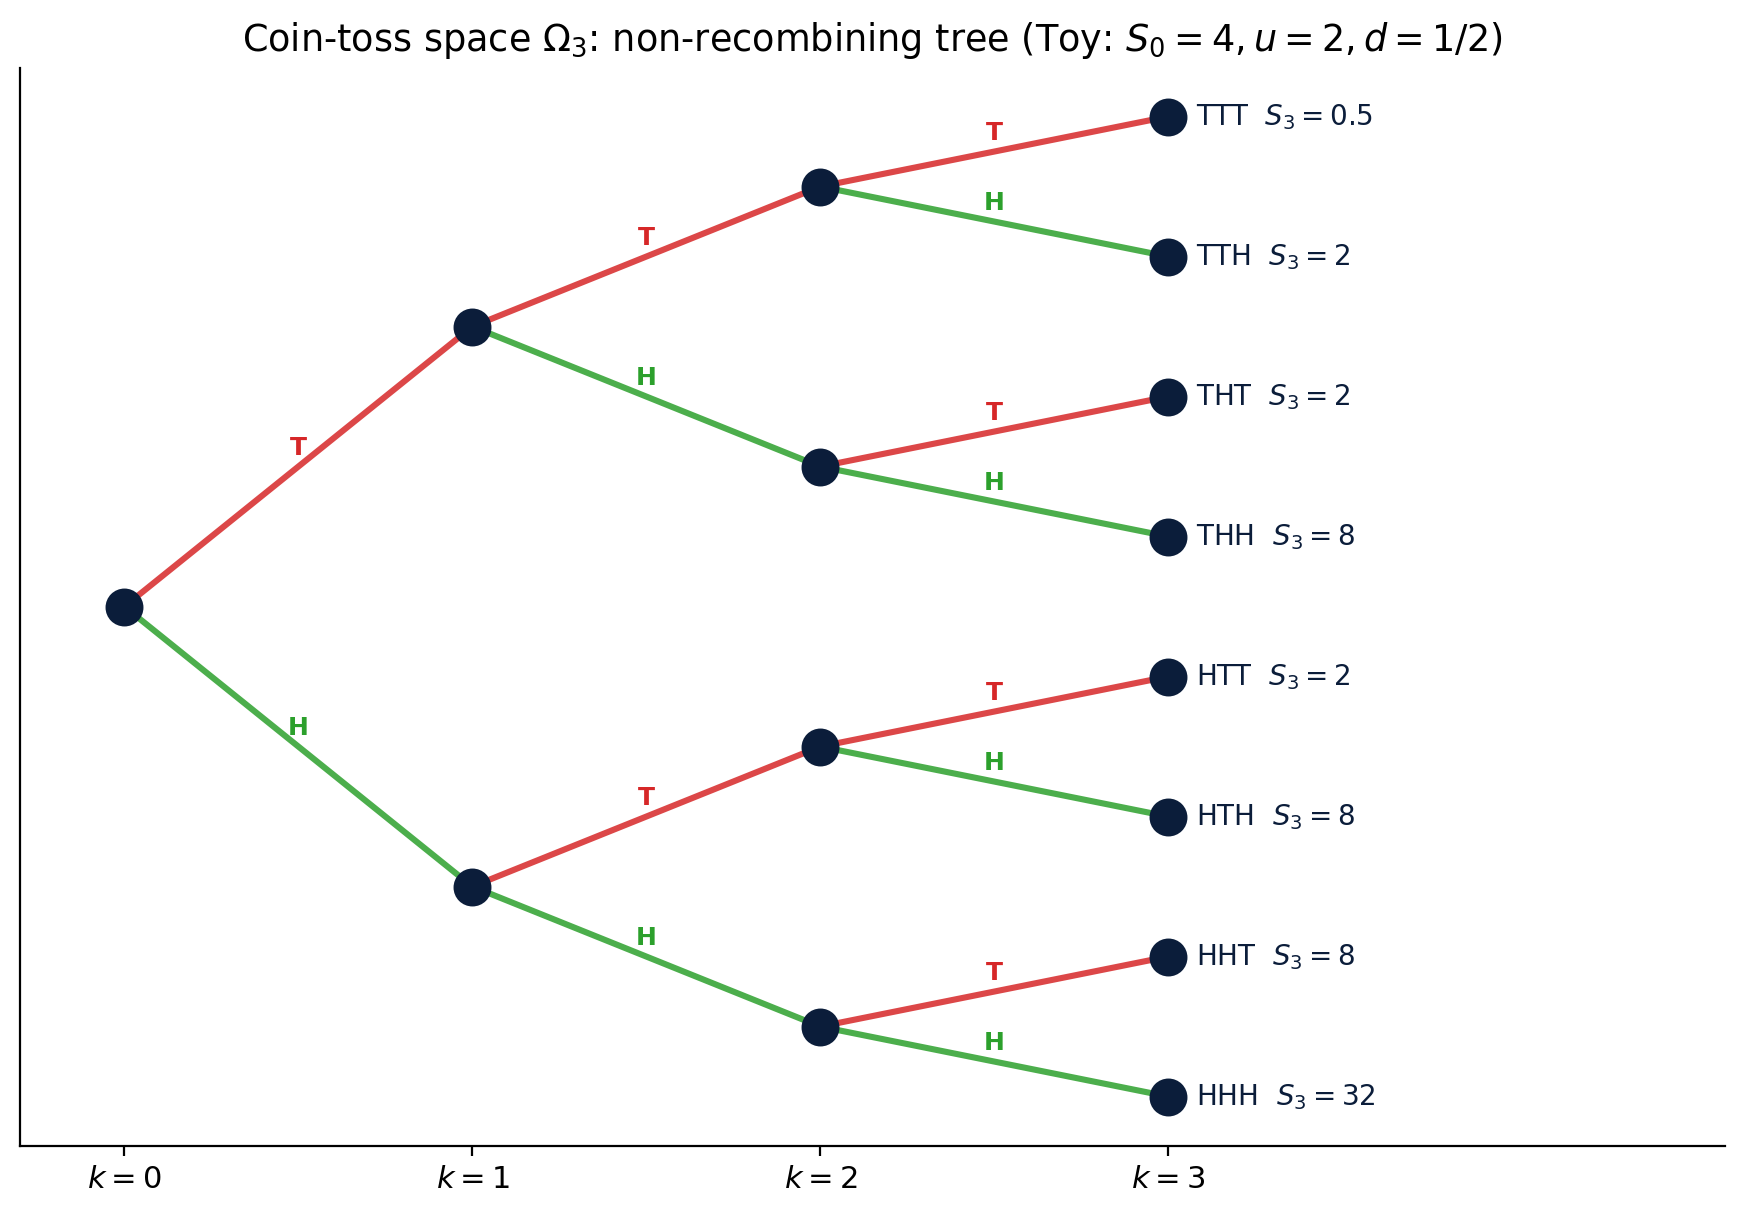
\includegraphics[keepaspectratio]{figures/ch03-omega-tree.png}}
\caption{The coin-toss space \(\Omega_3\) drawn as a non-recombining
binary tree. Eight leaves, each labelled with its three-letter
\(\omega\)-word and the resulting \(S_3\). Green edges = \(H\) (up), red
= \(T\) (down). Two words can end at the same \(S_3\) value (here
\(HHT\), \(HTH\), \(THH\) all give \(S_3=8\)).}
\end{figure}

\begin{figure}
\centering
\pandocbounded{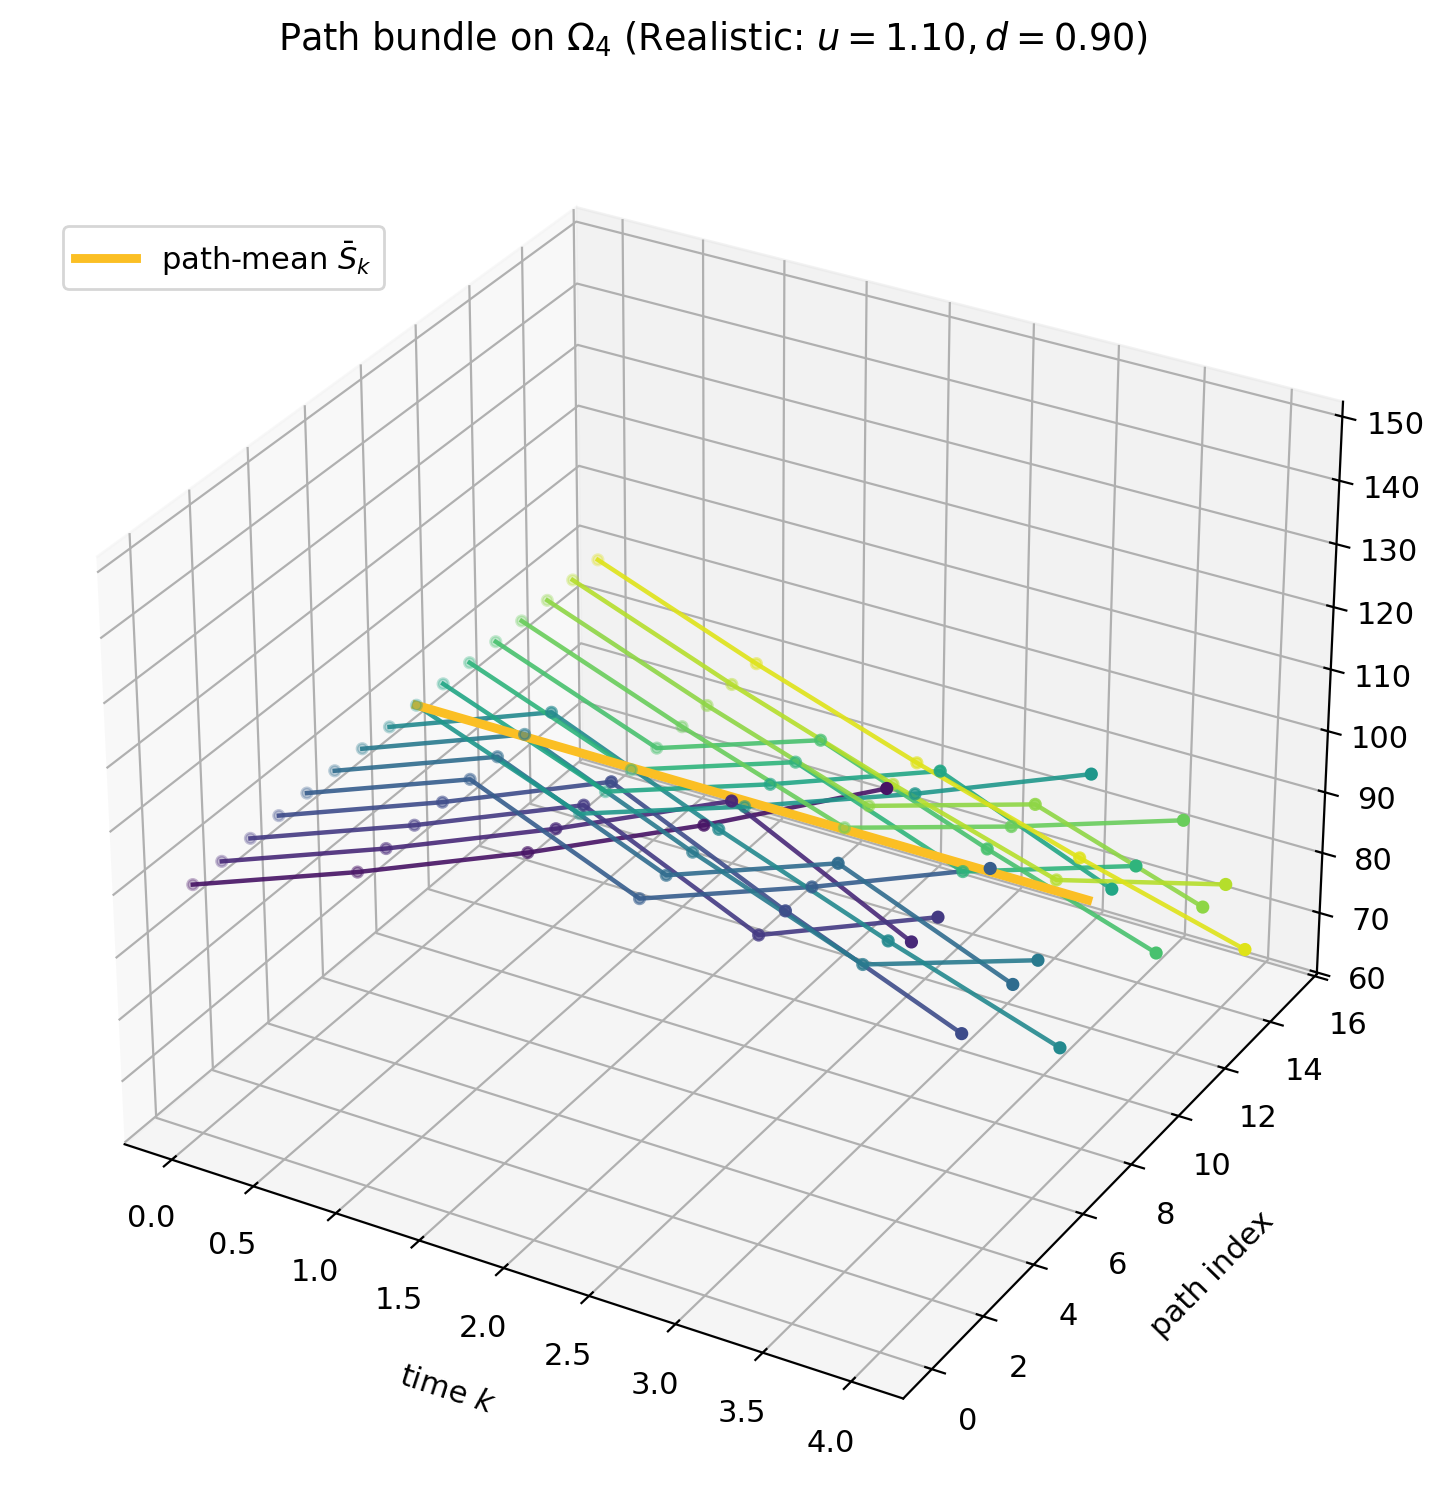
\includegraphics[keepaspectratio]{figures/ch03-pathbundle-3d.png}}
\caption{All sixteen paths of \(\Omega_4\) plotted in 3-D: \(x=\) time
\(k\), \(y=\) path index, \(z=\) price \(S_k\). Realistic parameters
(\(u=1.10\), \(d=0.90\)). The bundle visualises \(\Omega_n\) as a set of
complete trajectories of a single function defined on \(\omega\).}
\end{figure}

\subsection{3.1.3 Table}\label{table-4}

\textbf{Table 3.1.} \(\Omega_3\) listing under the toy. Each row is one
sample point.

{\def\LTcaptype{none} % do not increment counter
\begin{table}[H]
\centering
\begin{tabular}{|l|c|c|c|r|r|r|r|}
\toprule
\(\omega\) & \(\omega_1\) & \(\omega_2\) & \(\omega_3\) & \(H_3\) & \(S_1\) & \(S_2\) & \(S_3\) \\
\midrule



\(HHH\) & H & H & H & 3 & 8 & 16 & 32 \\
\(HHT\) & H & H & T & 2 & 8 & 16 & 8 \\
\(HTH\) & H & T & H & 2 & 8 & 4 & 8 \\
\(HTT\) & H & T & T & 1 & 8 & 4 & 2 \\
\(THH\) & T & H & H & 2 & 2 & 4 & 8 \\
\(THT\) & T & H & T & 1 & 2 & 4 & 2 \\
\(TTH\) & T & T & H & 1 & 2 & 1 & 2 \\
\(TTT\) & T & T & T & 0 & 2 & 1 & 0.5 \\
\bottomrule
\end{tabular}
\end{table}
}

\begin{center}\rule{0.5\linewidth}{0.5pt}\end{center}

\section{§3.2 Events as subsets}\label{events-as-subsets}

\textbf{Punchline.} An \emph{event} is a set of paths. Its probability
is the sum of the leaf weights inside that set. Nothing more
sophisticated than that.

\textbf{Intuition.} ``The stock ends above 100'' is a sentence in
English. The mathematical version is ``the subset \(A \subset \Omega_n\)
of those \(\omega\) for which \(S_n(\omega) > 100\)''. A probability
measure \(\mathbb P\) assigns weight \(\mathbb P(\{\omega\})\) to each
singleton; the event probability is

\[\mathbb P(A) \;=\; \sum_{\omega \in A} \mathbb P(\{\omega\}).\]

Two events \(A,B\) relate by union, intersection, complement; their
probabilities combine by the usual inclusion-exclusion. Because
\(\Omega_n\) is finite there is no measure-theoretic subtlety to worry
about.

\subsection{3.2.1 Definitions}\label{definitions-7}

\begin{itemize}
\tightlist
\item
  \textbf{Event}: any \(A \subseteq \Omega_n\).
\item
  \textbf{Probability measure} under \(\mathbb P\) (real-world,
  parameter \(p\)): for \(\omega\) with \(H_n(\omega) = j\),
  \[\mathbb P(\{\omega\}) = p^{\,j}\,(1-p)^{\,n-j}.\]
\item
  \textbf{Probability measure} under \(\tilde{\mathbb P}\)
  (risk-neutral, parameter \(\tilde p\)): same formula with
  \(\tilde p\).
\item
  \textbf{Event probability}:
  \(\mathbb P(A) = \sum_{\omega \in A} \mathbb P(\{\omega\})\).
\end{itemize}

Both \(\mathbb P\) and \(\tilde{\mathbb P}\) are well-defined
probability measures: leaf weights are non-negative and sum to 1 by the
binomial theorem.

\subsection{3.2.2 Examples}\label{examples-12}

\textbf{Example 3.2.1 (\(\tilde{\mathbb P}(S_2 = 16)\) on Toy,
\(n=2\)).} \(\{S_2 = 16\} = \{HH\}\), single element.
\(\tilde{\mathbb P}(\{HH\}) = (1/2)^2 = 1/4\).

\textbf{Example 3.2.2 (\(\tilde{\mathbb P}(S_2 = 4)\) on Toy, \(n=2\)).}
\(\{S_2 = 4\} = \{HT, TH\}\), two elements.
\(\tilde{\mathbb P} = 2 \cdot (1/2)^2 = 1/2\).

\textbf{Example 3.2.3 (\(\tilde{\mathbb P}(S_2 = 1)\) on Toy, \(n=2\)).}
\(\{TT\}\), single element. \(\tilde{\mathbb P} = 1/4\). The three event
probabilities sum to 1 as required.

\textbf{Example 3.2.4 (Same event, two measures).} Under real-world
\(p = 0.6\): \(\mathbb P(S_2 = 16) = 0.36\),
\(\mathbb P(S_2 = 4) = 0.48\), \(\mathbb P(S_2 = 1) = 0.16\). The
distribution shifts up because heads are more likely. Same event,
\emph{different probability} --- this is the whole point of §3.11.

\textbf{Example 3.2.5 (Realistic \(\tilde{\mathbb P}(S_3 \ge 108)\)).}
\(\tilde p = 0.6\), \(n=3\). The event
\(\{S_3 \ge 108\} = \{\omega : H_3(\omega) \ge 2\}\) (since
\(S_3 = 100 \cdot 1.1^j \cdot 0.9^{3-j}\) exceeds 108 iff \(j \ge 2\)).
Mass:

\[
\begin{aligned}
\tilde{\mathbb P}(H_3 \ge 2)
&= \binom{3}{2}\,\tilde p^2\,(1-\tilde p) + \binom{3}{3}\,\tilde p^3 \\
&= 3(0.36)(0.4) + 0.216 \;=\; 0.432 + 0.216 \;=\; 0.648.
\end{aligned}
\]

So \(\tilde{\mathbb P}(S_3 \ge 108) = 0.648\).

\textbf{Example 3.2.6 (Union of disjoint events).} On \(n=2\),
\(A = \{S_2 \ne 4\} = \{HH, TT\}\).
\(\tilde{\mathbb P}(A) = 1/4 + 1/4 = 1/2\). As a sanity check,
\(A^c = \{HT, TH\}\) has \(\tilde{\mathbb P}(A^c) = 1/2\), and
\(\tilde{\mathbb P}(A) + \tilde{\mathbb P}(A^c) = 1\). ✓

\textbf{Example 3.2.7 (Inclusion-exclusion on \(\Omega_3\)).} Let
\(A = \{\omega_1 = H\}\) and \(B = \{H_3 \ge 2\}\). Then
\(A \cap B = \{HHH, HHT, HTH, THH\} \cap \{H_3 \ge 2\}\) --- actually
\(A \cap B = \{HHH, HHT, HTH\}\) (each starts with \(H\) and has
\(\ge 2\) heads). Under \(\tilde{\mathbb P}=0.5\):
\(\tilde{\mathbb P}(A) = 1/2\), \(\tilde{\mathbb P}(B) = 4/8 = 1/2\),
\(\tilde{\mathbb P}(A \cap B) = 3/8\), so
\(\tilde{\mathbb P}(A \cup B) = 1/2 + 1/2 - 3/8 = 5/8\).

\textbf{Example 3.2.8 (Independence test, \(\omega_1\) and
\(\omega_3\)).} Under \(\tilde{\mathbb P}\) on \(\Omega_3\), the events
\(\{\omega_1 = H\}\) and \(\{\omega_3 = H\}\) each have mass \(1/2\),
and their intersection has \(\{HHH, HTH\}\), mass
\(1/4 = 1/2 \cdot 1/2\). Independent. ✓ (Recall: i.i.d. tosses is built
into the model.)

\begin{figure}
\centering
\pandocbounded{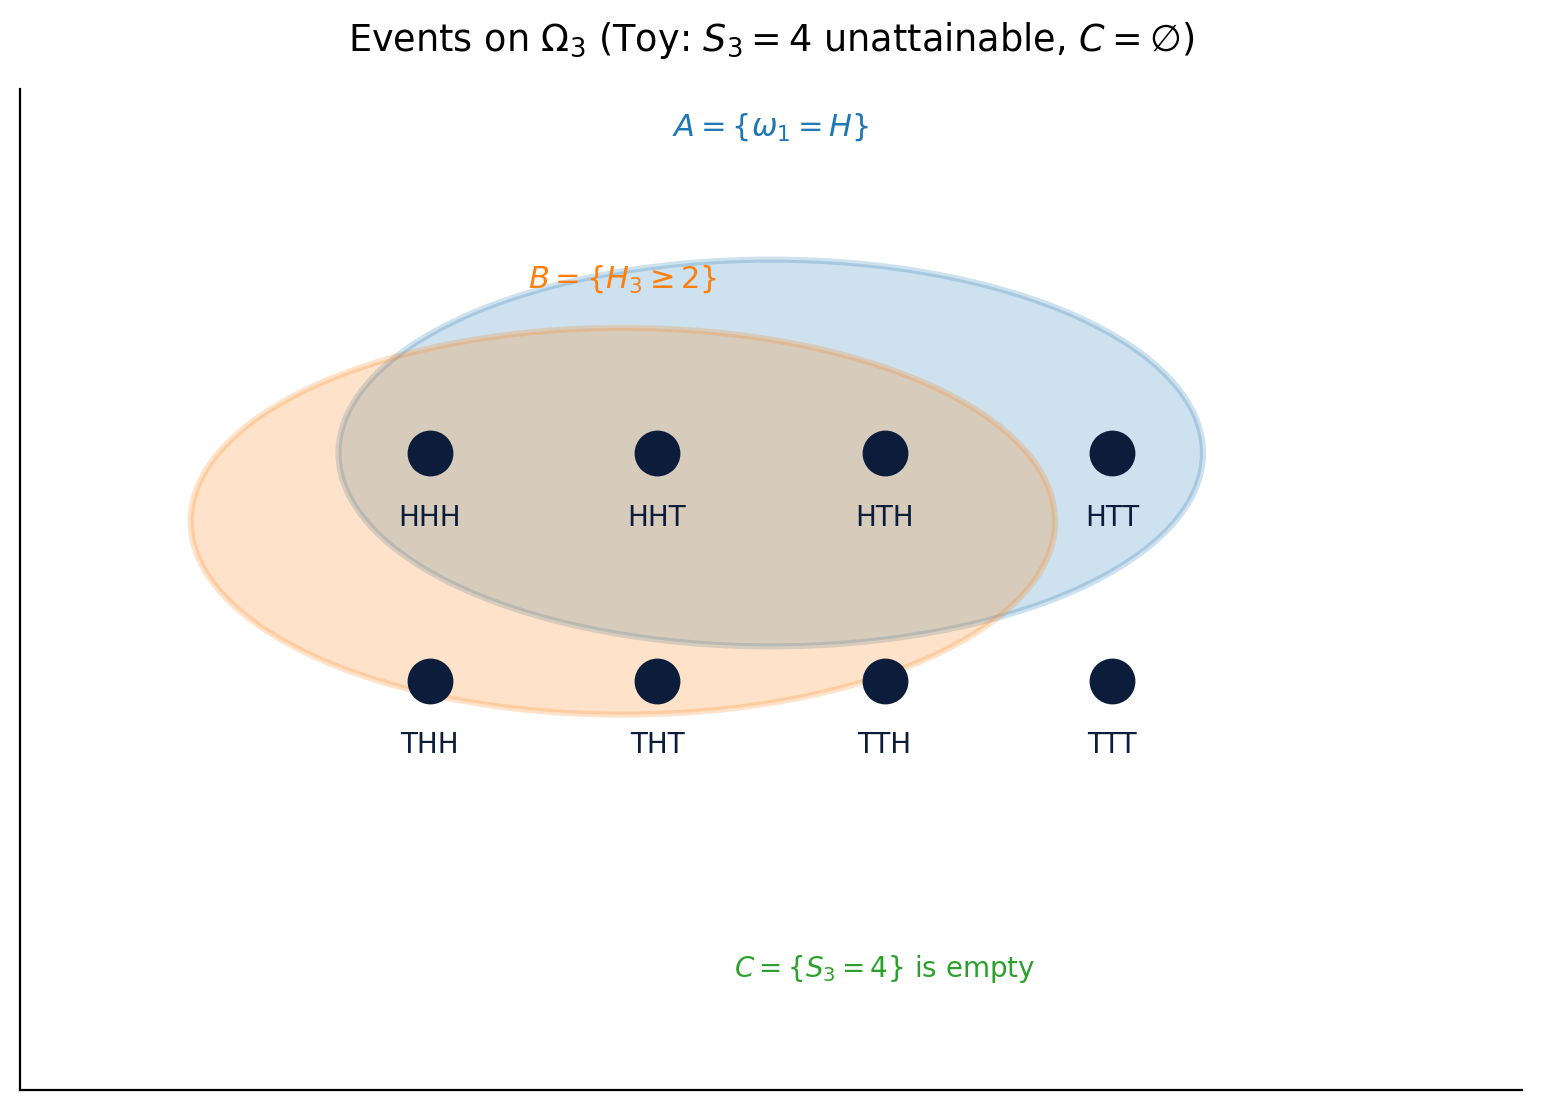
\includegraphics[keepaspectratio]{figures/ch03-event-venn.png}}
\caption{Venn-diagram style picture of \(\Omega_3\) with three coloured
events: \(A = \{\omega_1 = H\}\) (blue), \(B = \{H_3 \ge 2\}\) (orange),
\(C = \{S_3 = 4\}\) on Toy (green, in fact empty as discussed in Example
3.1.4). Each leaf \(\omega\) is a node; the coloured blobs cover all
leaves belonging to that event.}
\end{figure}

\begin{figure}
\centering
\pandocbounded{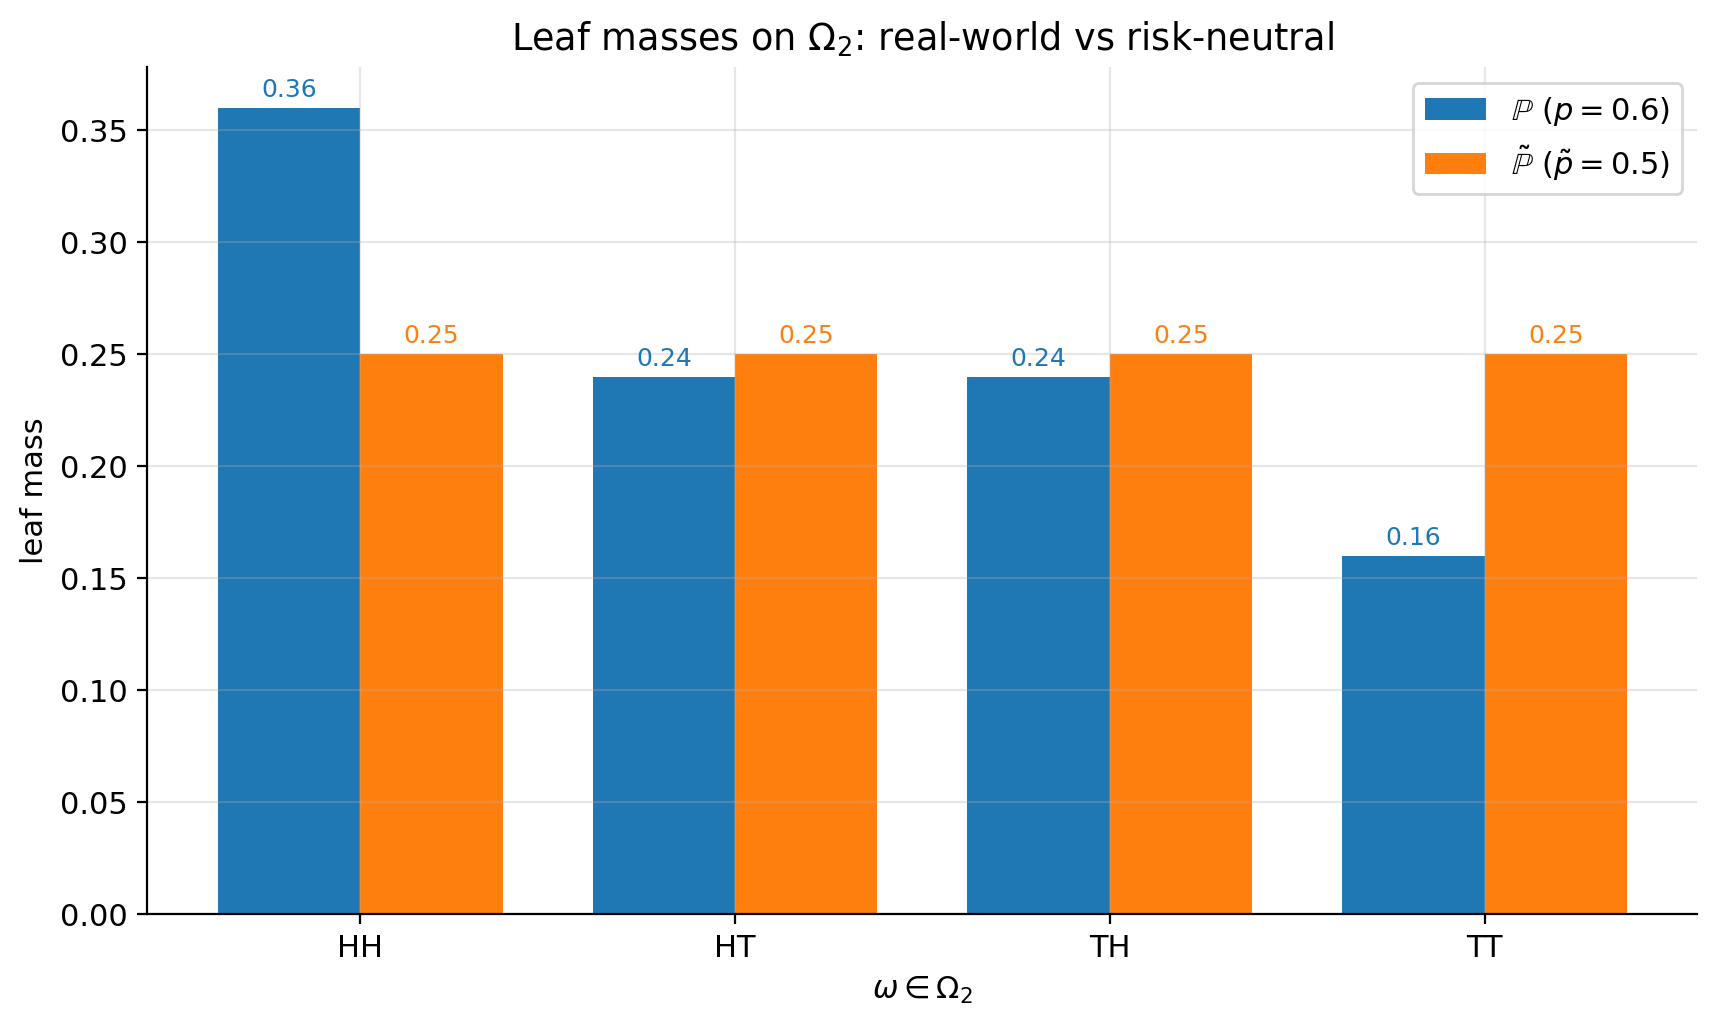
\includegraphics[keepaspectratio]{figures/ch03-leaf-masses.png}}
\caption{Leaf masses on \(\Omega_2\): real-world \(\mathbb P\) with
\(p = 0.6\) (blue) vs risk-neutral \(\tilde{\mathbb P}\) with
\(\tilde p = 0.5\) (orange). Same four leaves, different weights. The
Radon-Nikodym derivative \(Z(\omega) = \tilde{\mathbb P}/\mathbb P\)
will be the ratio of these heights.}
\end{figure}

\subsection{3.2.3 Table}\label{table-5}

\textbf{Table 3.2.} A handful of events on \(\Omega_3\) under the toy.

{\def\LTcaptype{none} % do not increment counter
\begin{table}[H]
\centering
\begin{tabular}{|l|l|r|r|}
\toprule
Event \(A\) & Members of \(A\) & \(\tilde{\mathbb P}(A)\) &
\(\mathbb P(A)\) \\
\midrule



\(\{S_3 = 32\}\) & \(HHH\) & \(1/8\) & \(0.216\) \\
\(\{S_3 = 8\}\) & \(HHT, HTH, THH\) & \(3/8\) & \(0.432\) \\
\(\{S_3 = 2\}\) & \(HTT, THT, TTH\) & \(3/8\) & \(0.288\) \\
\(\{S_3 = 0.5\}\) & \(TTT\) & \(1/8\) & \(0.064\) \\
\(\{\omega_1 = H\}\) & \(A_H\) (4 paths) & \(1/2\) & \(0.6\) \\
\(\{H_3 \ge 2\}\) & \(HHH, HHT, HTH, THH\) & \(1/2\) & \(0.648\) \\
\(\{S_1=2,\,S_3=2\}\) & \(THT, TTH\) & \(1/4\) & \(0.192\) \\
\bottomrule
\end{tabular}
\end{table}
}

\emph{Note.} \(\mathbb P(A)\) uses real-world \(p=0.6\). Row 7: among
\(T\)-prefix paths (\(S_1=2\)), both \(THT\) and \(TTH\) end at
\(S_3=2\) (each has exactly one \(H\) in \(\omega_2\omega_3\), giving
\(S_3 = 2 \cdot u \cdot d = 2\)); the path \(THH\) has \(S_1=2\) but
\(S_3=8\), and \(TTT\) has \(S_3=0.5\). Each of \(THT, TTH\) has
\(\mathbb P\)-mass \(0.6 \cdot 0.4^2 = 0.096\), so the row sums to
\(0.192\). \(A_H = \{HHH, HHT, HTH, HTT\}\).

\begin{center}\rule{0.5\linewidth}{0.5pt}\end{center}

\section{§3.3 Filtrations as nested
partitions}\label{filtrations-as-nested-partitions}

\textbf{Punchline.} \(\mathcal F_k\) is your eyesight at time \(k\). You
can tell apart any two sample points that disagree in the first \(k\)
flips, but you \emph{cannot} tell apart those that agree in the first
\(k\) flips and only differ later. A filtration is the chronological
refinement of this eyesight.

\textbf{Intuition.} At time \(k=0\) you have observed nothing; the
universe is one giant block, \(\Omega_n\). After one flip, you can tell
apart ``started with \(H\)'' from ``started with \(T\)''. After two
flips, you can tell apart all four two-letter prefixes. After \(n\)
flips, you can tell apart every word. Each \(\mathcal F_k\) is a
\emph{partition} of \(\Omega_n\), and the partitions get finer as \(k\)
grows. That refinement is the filtration.

Two equivalent ways to describe \(\mathcal F_k\):

\begin{itemize}
\tightlist
\item
  As a partition: blocks are equivalence classes of ``agrees in the
  first \(k\) letters''. There are \(2^k\) blocks, each of size
  \(2^{n-k}\).
\item
  As a \(\sigma\)-algebra (we won't need this language much): the events
  that are unions of \(\mathcal F_k\)-blocks.
\end{itemize}

We work entirely with the \emph{partition} picture. It is concrete,
finite, and intuitive.

\subsection{3.3.1 Definitions}\label{definitions-8}

For \(n\) fixed and \(0 \le k \le n\), define an equivalence relation on
\(\Omega_n\):

\[\omega \sim_k \omega' \quad\Longleftrightarrow\quad \omega_i = \omega_i' \text{ for } i = 1, \ldots, k.\]

The \textbf{filtration} \(\mathbb F = (\mathcal F_k)_{k=0}^n\) is the
sequence of partitions induced by these equivalences. Equivalently,
\(\mathcal F_k\) is the set of events that are \emph{unions of
\(\sim_k\) equivalence classes}.

\begin{itemize}
\tightlist
\item
  \(\mathcal F_0 = \{\emptyset, \Omega_n\}\): one block of size \(2^n\).
  You see nothing.
\item
  \(\mathcal F_k\): \(2^k\) blocks each of size \(2^{n-k}\). You see the
  first \(k\) flips.
\item
  \(\mathcal F_n\): \(2^n\) singletons. You see everything.
\end{itemize}

The \emph{nesting} is the key:

\[\mathcal F_0 \subset \mathcal F_1 \subset \cdots \subset \mathcal F_n.\]

This containment is in the \(\sigma\)-algebra sense (every
\(\mathcal F_k\)-event is also an \(\mathcal F_{k+1}\)-event) or in the
partition sense (every \(\mathcal F_k\)-block is a union of
\(\mathcal F_{k+1}\)-blocks, two of them in fact).

\subsection{3.3.2 Examples}\label{examples-13}

\textbf{Example 3.3.1 (\(\mathcal F_0\) on \(\Omega_3\)).} One block:
\(\Omega_3\) itself. You haven't flipped yet.

\textbf{Example 3.3.2 (\(\mathcal F_1\) on \(\Omega_3\)).} Two blocks:

\begin{itemize}
\tightlist
\item
  \(A_H = \{HHH, HHT, HTH, HTT\}\) --- words starting with \(H\).
\item
  \(A_T = \{THH, THT, TTH, TTT\}\) --- words starting with \(T\).
\end{itemize}

\textbf{Example 3.3.3 (\(\mathcal F_2\) on \(\Omega_3\)).} Four blocks,
by two-letter prefix:

\begin{itemize}
\tightlist
\item
  \(A_{HH} = \{HHH, HHT\}\)
\item
  \(A_{HT} = \{HTH, HTT\}\)
\item
  \(A_{TH} = \{THH, THT\}\)
\item
  \(A_{TT} = \{TTH, TTT\}\)
\end{itemize}

\textbf{Example 3.3.4 (\(\mathcal F_3\) on \(\Omega_3\)).} Eight
singletons: each word is its own block.

\textbf{Example 3.3.5 (Verify \(\mathcal F_1 \subset \mathcal F_2\)).}
\(A_H = A_{HH} \cup A_{HT}\) --- yes, \(\mathcal F_1\)-block \(A_H\) is
a union of two \(\mathcal F_2\)-blocks. Similarly
\(A_T = A_{TH} \cup A_{TT}\). So every \(\mathcal F_1\)-event (which is
a union of \(\mathcal F_1\)-blocks) is also a union of
\(\mathcal F_2\)-blocks, hence an \(\mathcal F_2\)-event. ✓

\textbf{Example 3.3.6 (Which block contains \(HTH\) in
\(\mathcal F_2\)?).} Prefix \(HT\), so \(A_{HT} = \{HTH, HTT\}\).

\textbf{Example 3.3.7 (Counting blocks on \(\Omega_4\)).}
\(\mathcal F_0\): 1 block size 16. \(\mathcal F_1\): 2 blocks of 8.
\(\mathcal F_2\): 4 blocks of 4. \(\mathcal F_3\): 8 blocks of 2.
\(\mathcal F_4\): 16 singletons. Doubling and halving each step.

\textbf{Example 3.3.8 (Block of \(\omega = HTHT\) in \(\mathcal F_2\)).}
Prefix \(HT\), block size \(2^{4-2} = 4\):
\(\{HTHH, HTHT, HTTH, HTTT\}\).

\textbf{Example 3.3.9 (Is \(\{S_2 = 4\}\) in \(\mathcal F_2\) on Toy,
\(n=3\)?).} Yes: \(\{S_2 = 4\} = A_{HT} \cup A_{TH}\) on \(\Omega_3\), a
union of two \(\mathcal F_2\)-blocks. Generally any event ``depending
only on the first \(k\) flips'' lives in \(\mathcal F_k\).

\textbf{Example 3.3.10 (Is \(\{S_3 = 8\}\) in \(\mathcal F_2\)?).} No:
this event = \(\{HHT, HTH, THH\}\). None of
\(A_{HH}, A_{HT}, A_{TH}, A_{TT}\) is a subset of \(\{S_3 = 8\}\), so
the event is \emph{not} a union of \(\mathcal F_2\)-blocks. Hence
\(\{S_3=8\} \notin \mathcal F_2\), which is intuitive: at time 2 you
don't yet know \(S_3\).

\begin{figure}
\centering
\pandocbounded{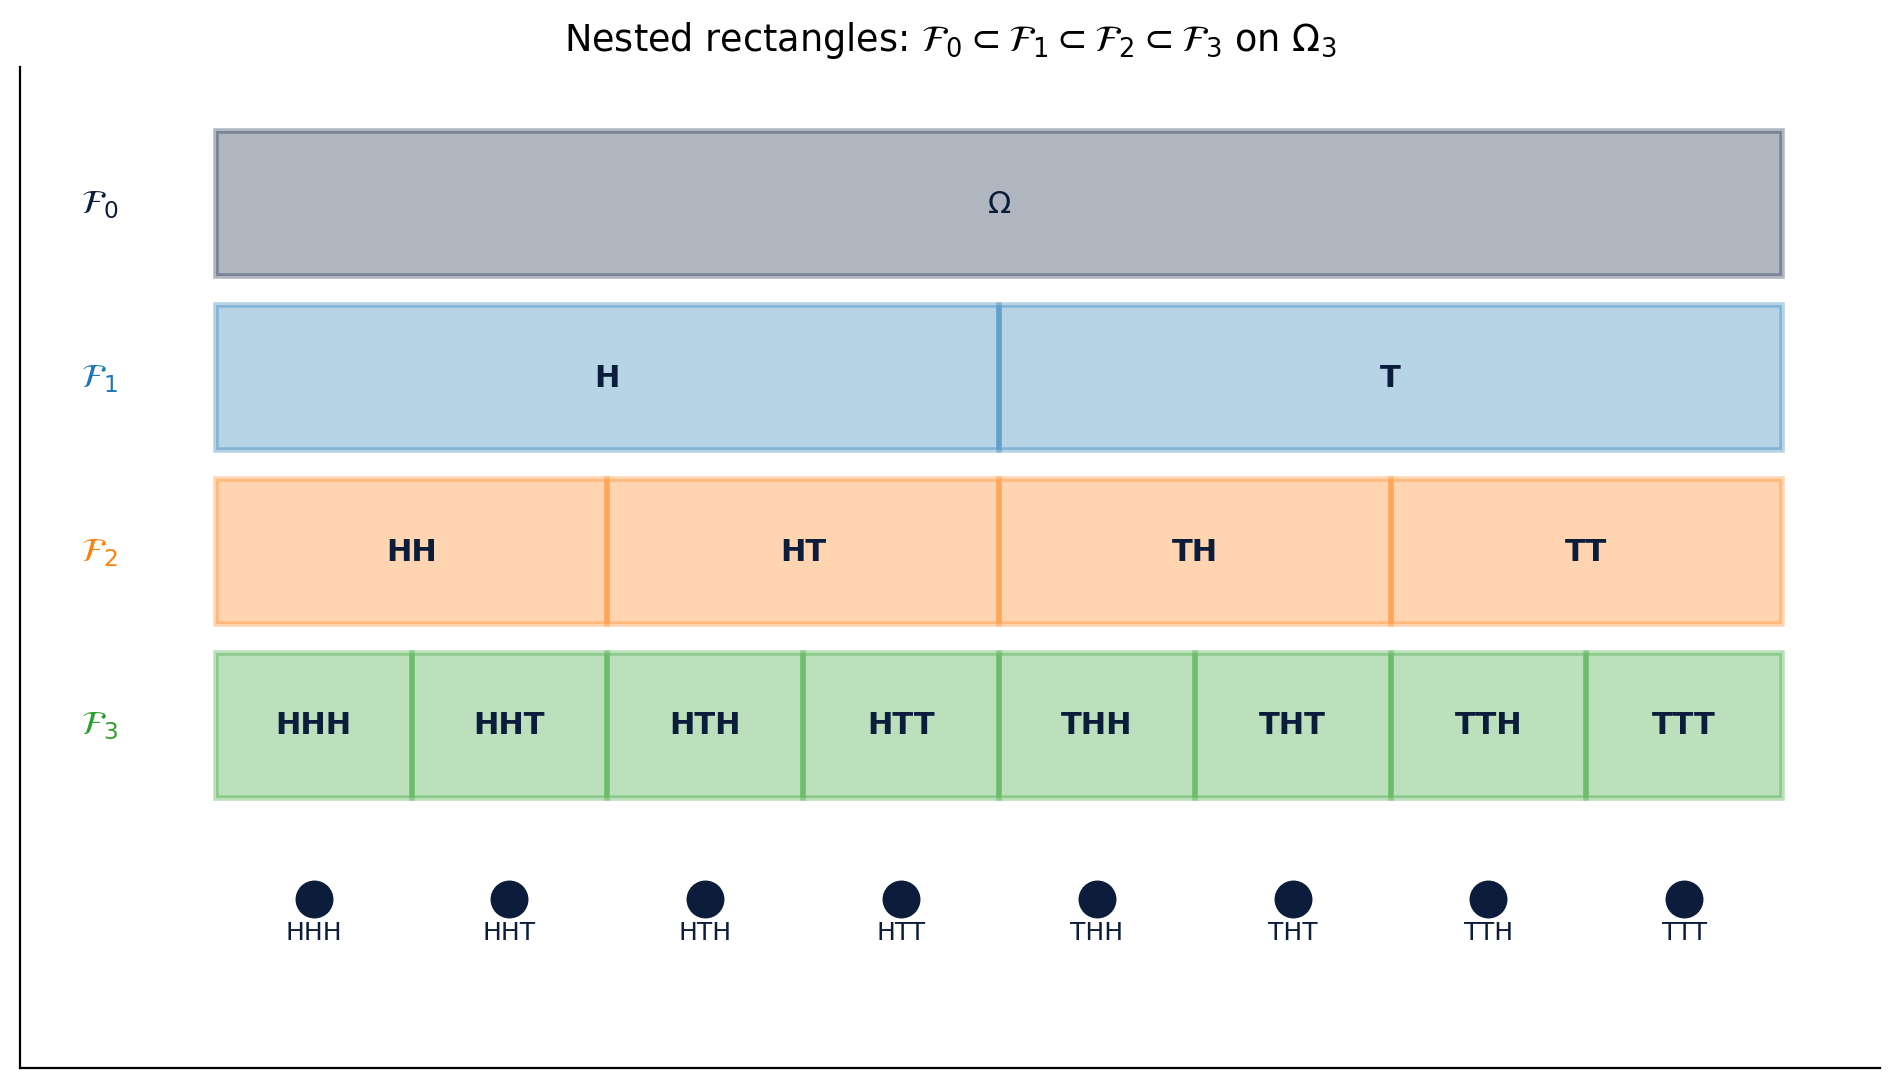
\includegraphics[keepaspectratio]{figures/ch03-nested-rectangles.png}}
\caption{Nested rectangles for \(\Omega_3\): the universal rectangle is
\(\mathcal F_0\). Splitting by first letter gives the two
\(\mathcal F_1\)-blocks. Splitting by first two letters gives four
\(\mathcal F_2\)-blocks. The bottom row of eight singletons is
\(\mathcal F_3\).}
\end{figure}

\begin{figure}
\centering
\pandocbounded{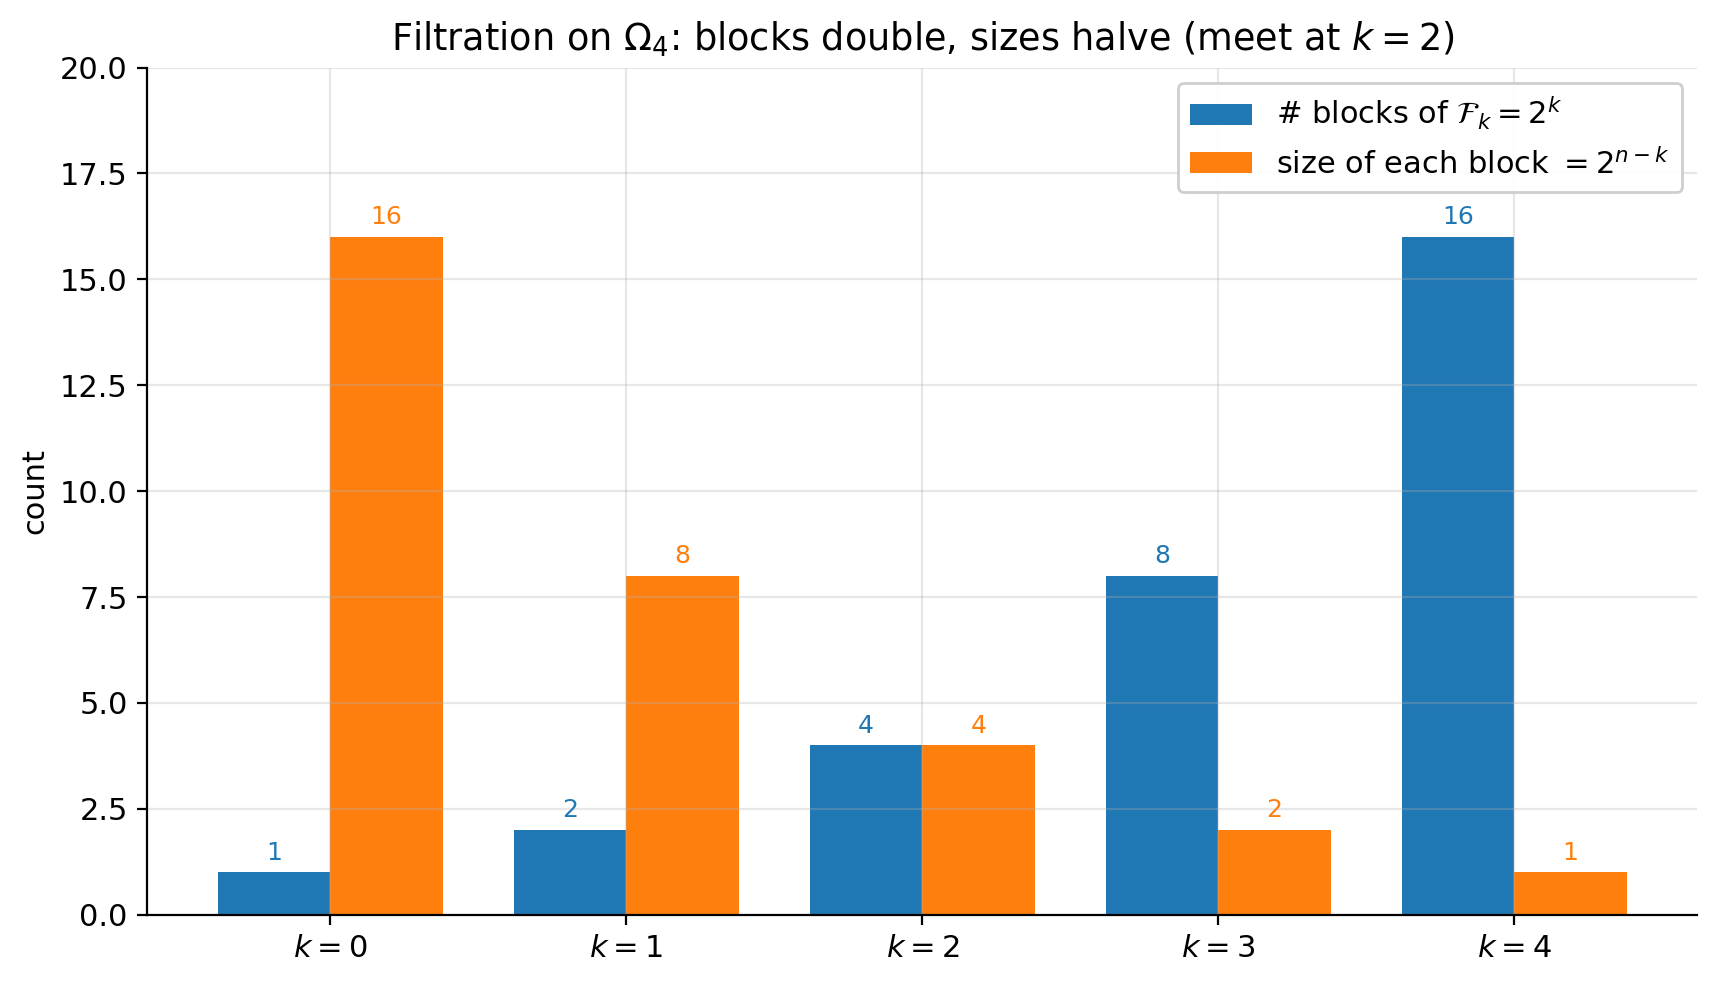
\includegraphics[keepaspectratio]{figures/ch03-Fk-blocks.png}}
\caption{Filtration on \(\Omega_4\) as a paired bar chart: number of
blocks of \(\mathcal F_k\) doubles as \(k\) grows; size of each block
halves. The two bars meet at \(k=2\) (\(4\) blocks of \(4\)).}
\end{figure}

\begin{figure}
\centering
\pandocbounded{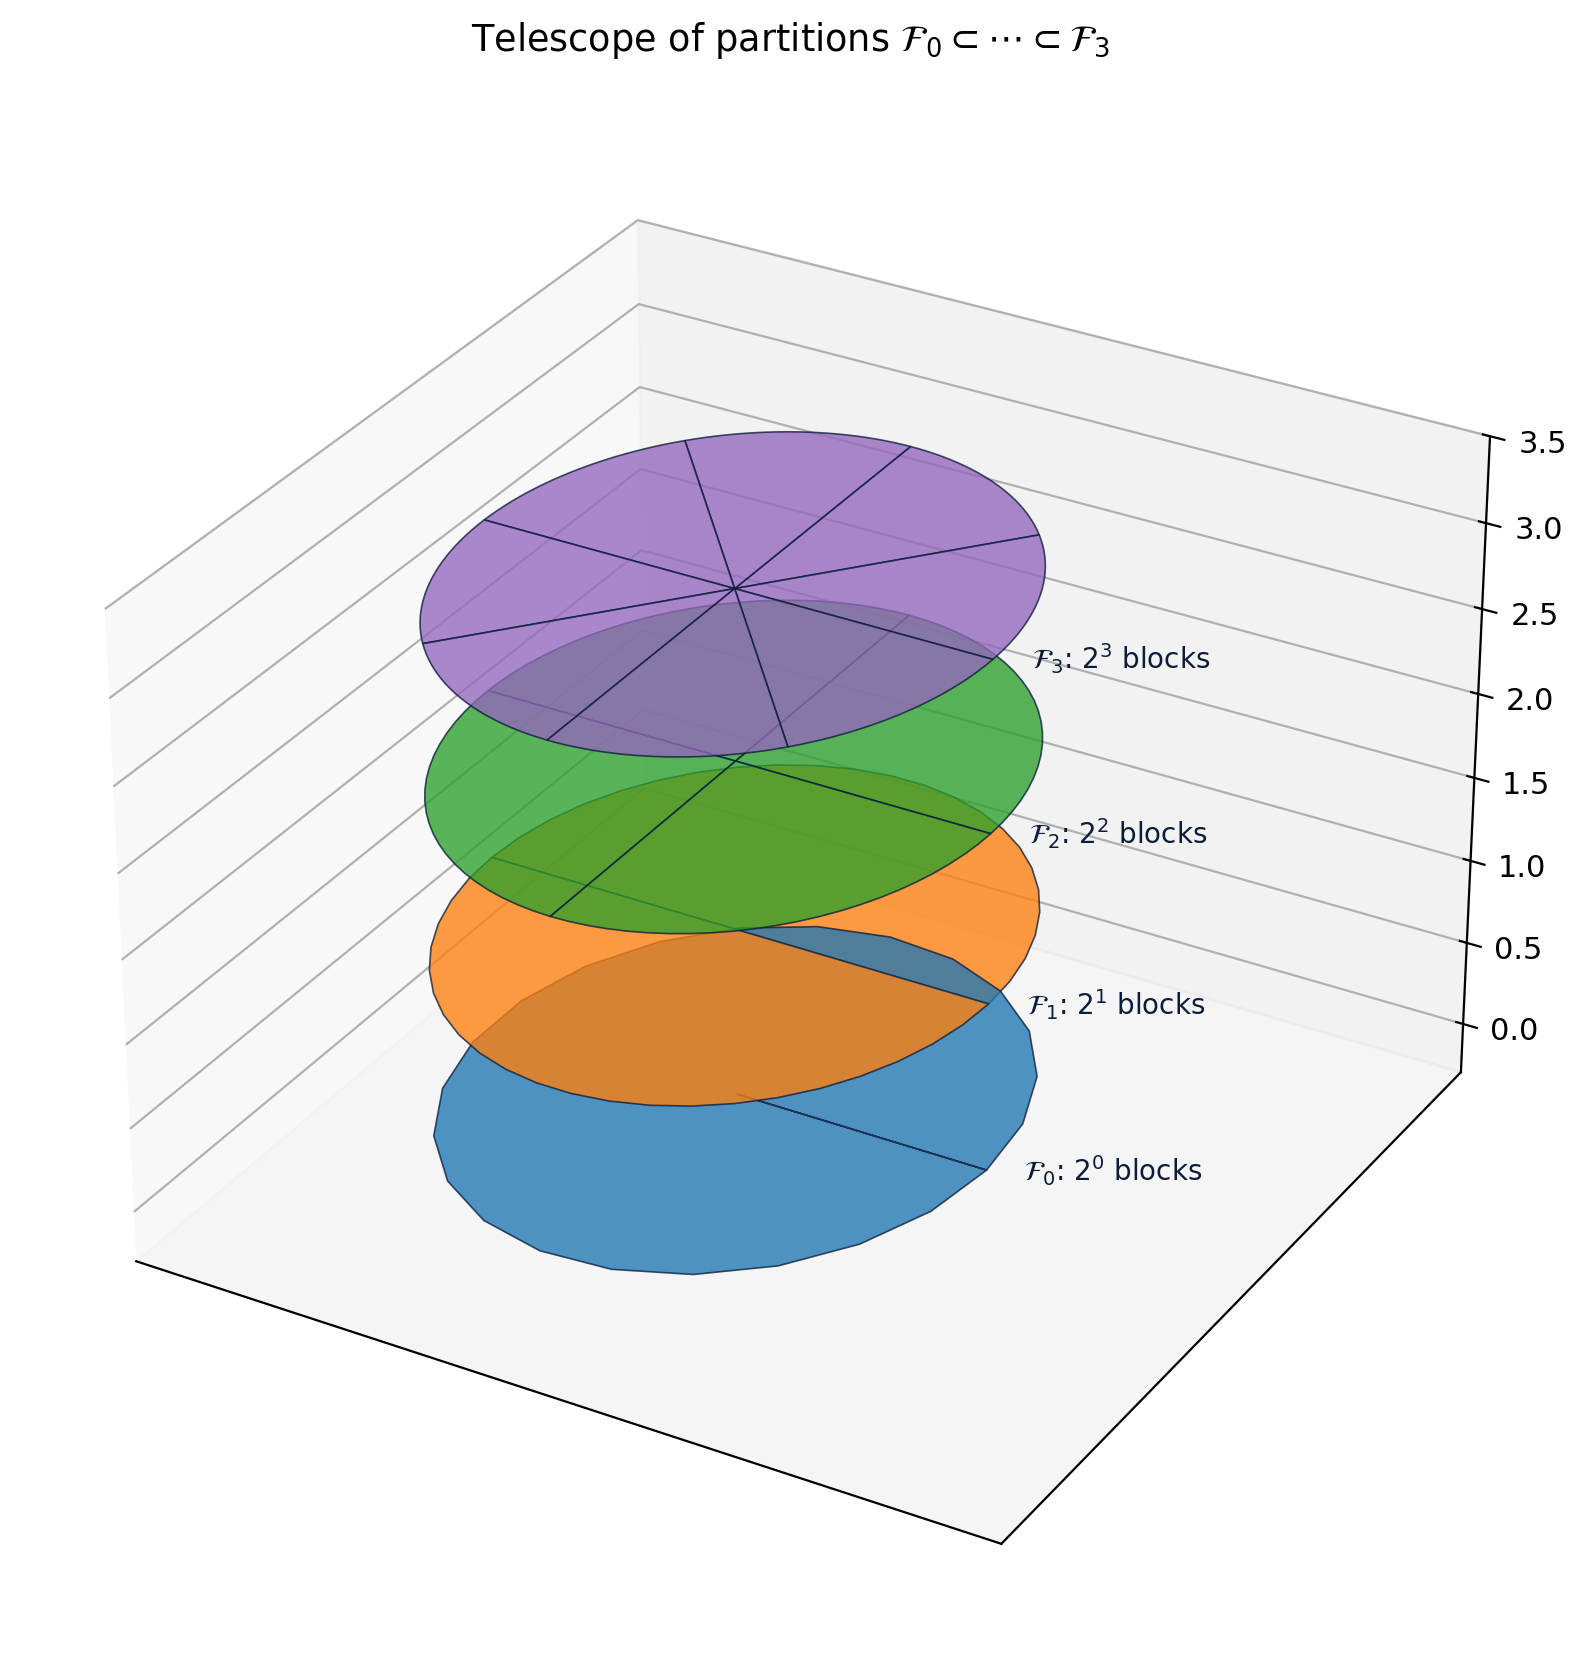
\includegraphics[keepaspectratio]{figures/ch03-telescope-partitions-3d.png}}
\caption{A 3-D ``telescope'' of partitions: discs stacked vertically,
each disc divided into \(2^k\) coloured wedges. Each wedge of disc \(k\)
is the union of two adjacent wedges of disc \(k+1\) --- the visual
content of \(\mathcal F_k \subset \mathcal F_{k+1}\).}
\end{figure}

\begin{figure}
\centering
\pandocbounded{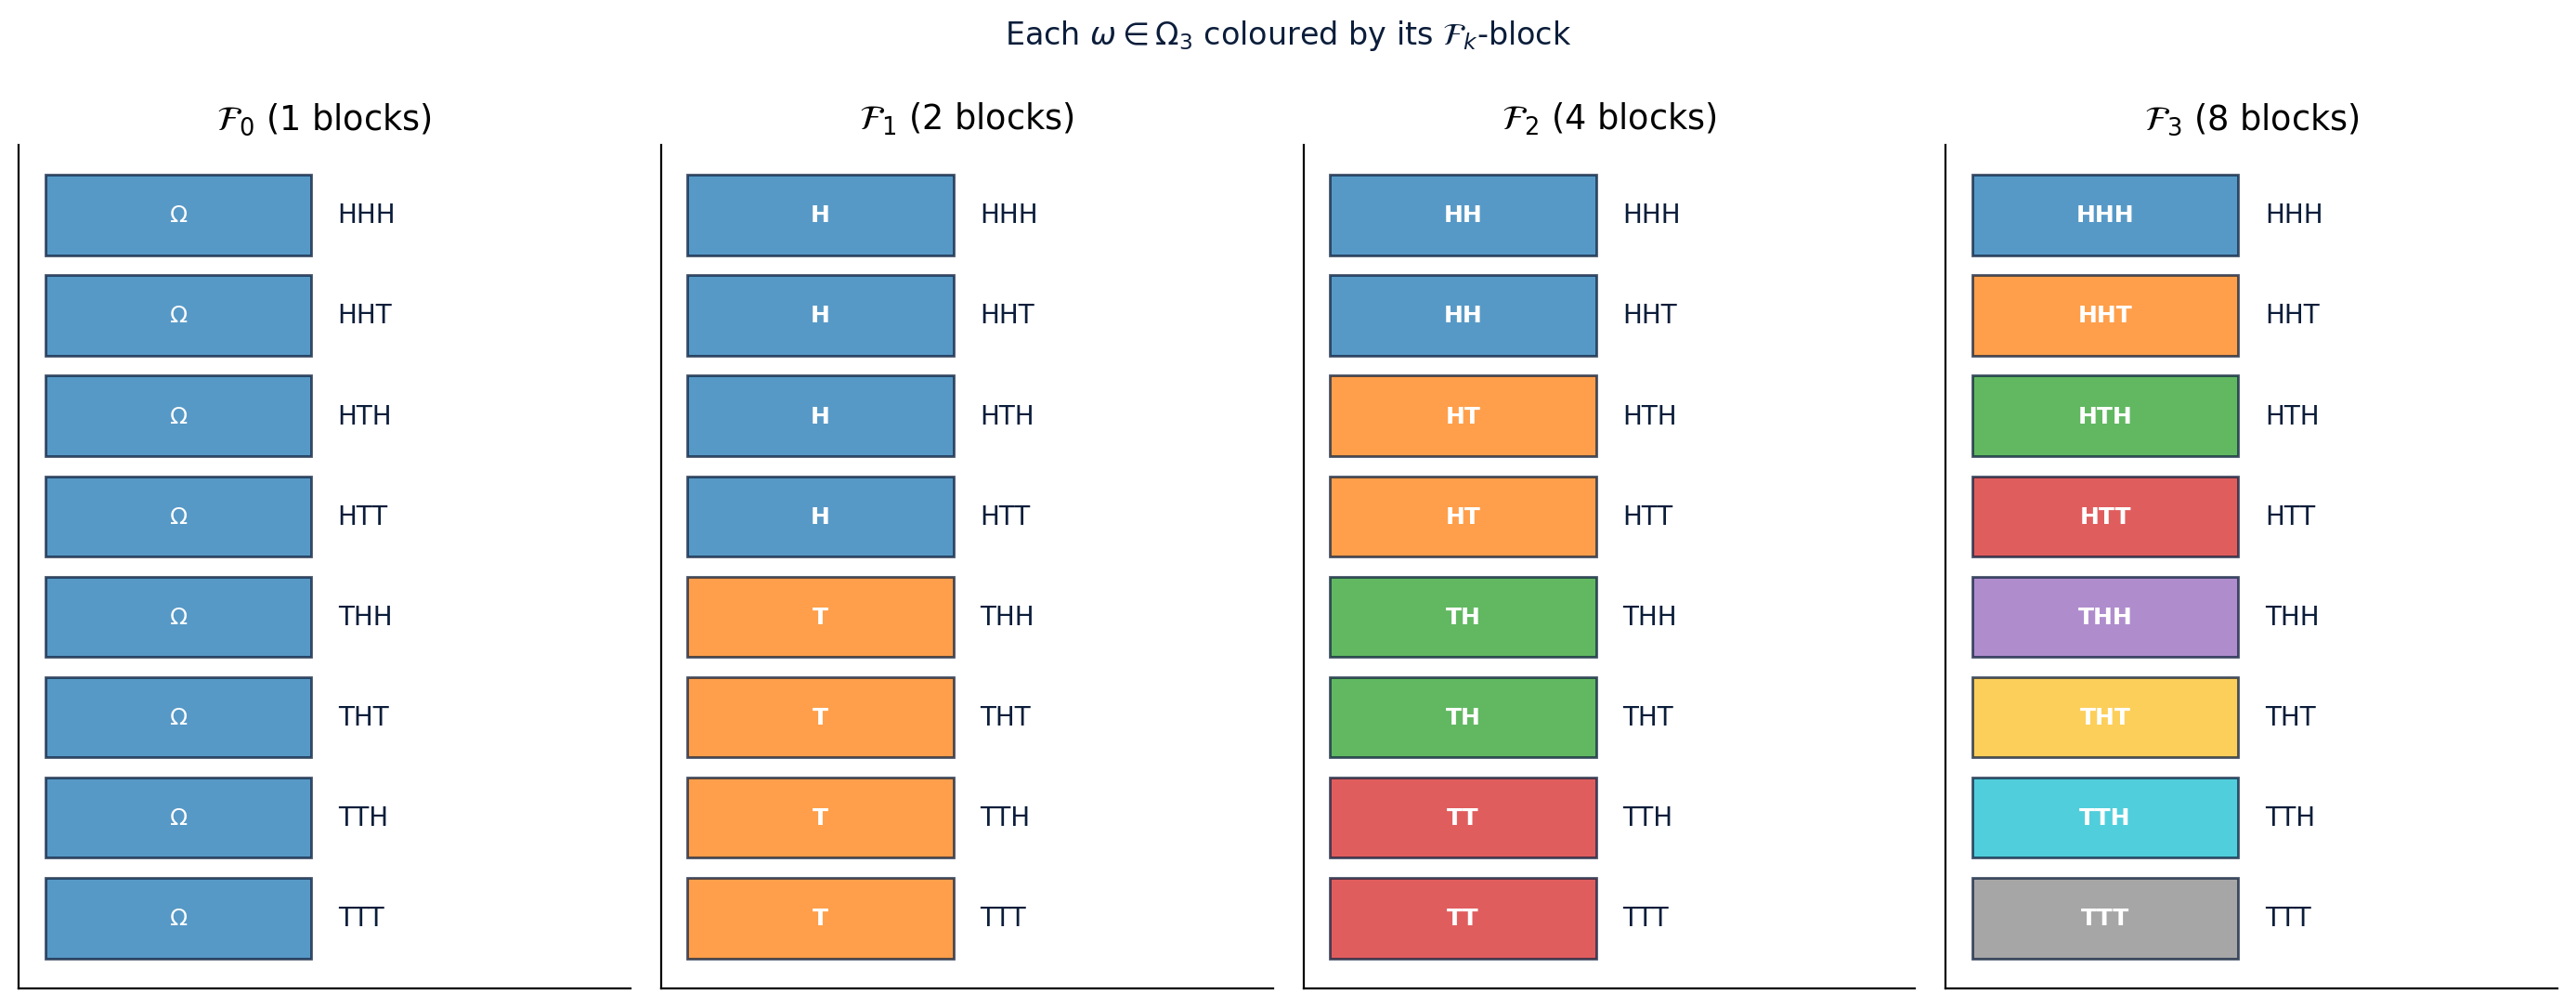
\includegraphics[keepaspectratio]{figures/ch03-Fk-colour-tree.png}}
\caption{Colour-by-block visualisation: four panels (for \(k=0,1,2,3\)
on \(\Omega_3\)). Each row is a leaf \(\omega\). The colour bar shows
which \(\mathcal F_k\)-block contains that leaf; the colouring becomes
finer as \(k\) grows.}
\end{figure}

\subsection{3.3.3 Table}\label{table-6}

\textbf{Table 3.3.} Filtration anatomy on \(\Omega_n\).

{\def\LTcaptype{none} % do not increment counter
\begin{table}[H]
\centering
\begin{tabular}{|r|r|r|l|}
\toprule
\(k\) & \# blocks of \(\mathcal F_k\) & size of each block & example block (\(n=3\)) \\
\midrule



0 & 1 & \(2^n\) & \(\Omega_n\) \\
1 & 2 & \(2^{n-1}\) & \(A_H, A_T\) \\
2 & 4 & \(2^{n-2}\) & \(A_{HH}, A_{HT}, A_{TH}, A_{TT}\) \\
\ldots{} & \ldots{} & \ldots{} & \ldots{} \\
\(n\) & \(2^n\) & \(1\) & singletons \\
\bottomrule
\end{tabular}
\end{table}
}

\begin{center}\rule{0.5\linewidth}{0.5pt}\end{center}

\section{§3.4 Random variables and
measurability}\label{random-variables-and-measurability}

\textbf{Punchline.} A random variable \(X\) is
\(\mathcal F_k\)-measurable iff \(X\) is \emph{constant on every block
of \(\mathcal F_k\)}. Equivalently: \(X\) depends only on the first
\(k\) flips.

\textbf{Intuition.} If at time \(k\) you only know the first \(k\)
flips, the only quantities you can compute are those that are determined
by the first \(k\) flips alone. A quantity that depends on the rest of
\(\omega\) --- for instance, \(S_{k+1}\) --- varies \emph{within} an
\(\mathcal F_k\)-block (because different leaves in the block correspond
to different futures). So \(S_{k+1}\) is not yet known at time \(k\),
and it is not \(\mathcal F_k\)-measurable.

This is the rigorous restatement of ``what you know at time \(k\)'': you
know \(X\) at time \(k\) iff \(X\) is a function of the first \(k\)
flips, iff \(X\) is constant on \(\mathcal F_k\)-blocks.

\subsection{3.4.1 Definitions}\label{definitions-9}

A \textbf{random variable} on \(\Omega_n\) is any function
\(X : \Omega_n \to \mathbb R\).

\(X\) is \textbf{\(\mathcal F_k\)-measurable} if for every
\(\mathcal F_k\)-block \(B\), \(X\) is constant on \(B\). Equivalently,
\(\{X \le x\} \in \mathcal F_k\) for every \(x \in \mathbb R\).

A useful re-statement: \(X\) is \(\mathcal F_k\)-measurable iff there is
a function \(g : \{H,T\}^k \to \mathbb R\) such that
\(X(\omega) = g(\omega_1, \ldots, \omega_k)\).

\subsection{3.4.2 Examples}\label{examples-14}

\textbf{Example 3.4.1 (\(S_2\) is \(\mathcal F_2\)-measurable, on
\(\Omega_3\)).} \(S_2(\omega) = S_0 u^{H_2} d^{2 - H_2}\) depends only
on \(\omega_1, \omega_2\). Constant on each \(\mathcal F_2\)-block. Pick
block \(A_{HT}\): \(S_2 = 4 \cdot 2 \cdot 0.5 = 4\) for both elements. ✓

\textbf{Example 3.4.2 (\(S_3\) is NOT \(\mathcal F_2\)-measurable).} On
block \(A_{HT} = \{HTH, HTT\}\): \(S_3(HTH) = 8\), \(S_3(HTT) = 2\). Not
constant on the block, so not \(\mathcal F_2\)-measurable.

\textbf{Example 3.4.3 (\(S_3\) IS \(\mathcal F_3\)-measurable).}
Trivially: \(\mathcal F_3\)-blocks are singletons, so any function is
constant on them.

\textbf{Example 3.4.4 (\(M_3 = \max(S_0, S_1, S_2, S_3)\) ---
measurability).} \(M_3\) depends on the whole path
\(\omega_1\omega_2\omega_3\), so it is \(\mathcal F_3\)-measurable. Is
it \(\mathcal F_2\)-measurable? Check on block \(A_{HT}\):
\(M_3(HTH) = \max(4, 8, 4, 8) = 8\) and
\(M_3(HTT) = \max(4, 8, 4, 2) = 8\). \emph{Constant on this block.} But
on block \(A_{HH}\): \(M_3(HHH) = 32\) and \(M_3(HHT) = 16\). Not
constant. So \(M_3 \notin \mathcal F_2\) in general. On specifically,
\(M_3\) is \(\mathcal F_3\)-measurable but not \(\mathcal F_2\).

\textbf{Example 3.4.5 (Constant \(X \equiv c\)).} Constant on the single
\(\mathcal F_0\)-block \(\Omega_n\). So a constant is
\(\mathcal F_0\)-measurable. In particular \(S_0\) is
\(\mathcal F_0\)-measurable.

\textbf{Example 3.4.6 (Indicator \(\mathbf 1_{\{\omega_1 = H\}}\)).}
Equals 1 on \(A_H\), 0 on \(A_T\). Constant on each
\(\mathcal F_1\)-block. So it is \(\mathcal F_1\)-measurable. (And not
\(\mathcal F_0\)-measurable: it takes two values.)

\textbf{Example 3.4.7 (Indicator \(\mathbf 1_{\{S_3 = 8\}}\)).} Equals 1
on \(\{HHT, HTH, THH\}\), 0 elsewhere. Constant on singletons, hence
\(\mathcal F_3\)-measurable. Not constant on \(\mathcal F_2\)-block
\(A_{HH}\) (where it equals 1 at \(HHT\) and 0 at \(HHH\)). Not
\(\mathcal F_2\)-measurable.

\textbf{Example 3.4.8 (\(\Delta_k\), the replicating-portfolio holding,
on \(n=2\)).} From Chapter 2,
\(\Delta_0 = \frac{V_1(H) - V_1(T)}{S_1(H) - S_1(T)}\) is a constant ---
\(\mathcal F_0\)-measurable. \(\Delta_1\) depends on whether we are at
the node \(H\) or \(T\) at time 1; it is constant on each
\(\mathcal F_1\)-block, hence \(\mathcal F_1\)-measurable. \emph{No
peeking} enters here as a measurability requirement on the hedge.

\textbf{Example 3.4.9 (Look-ahead \(Y_k = S_{k+1}\)).} On \(A_{HT}\):
\(Y_2(HTH) = 8\), \(Y_2(HTT) = 2\). Not \(\mathcal F_2\)-measurable. The
look-ahead is a peek into the future and the maths confirms it.

\begin{figure}
\centering
\pandocbounded{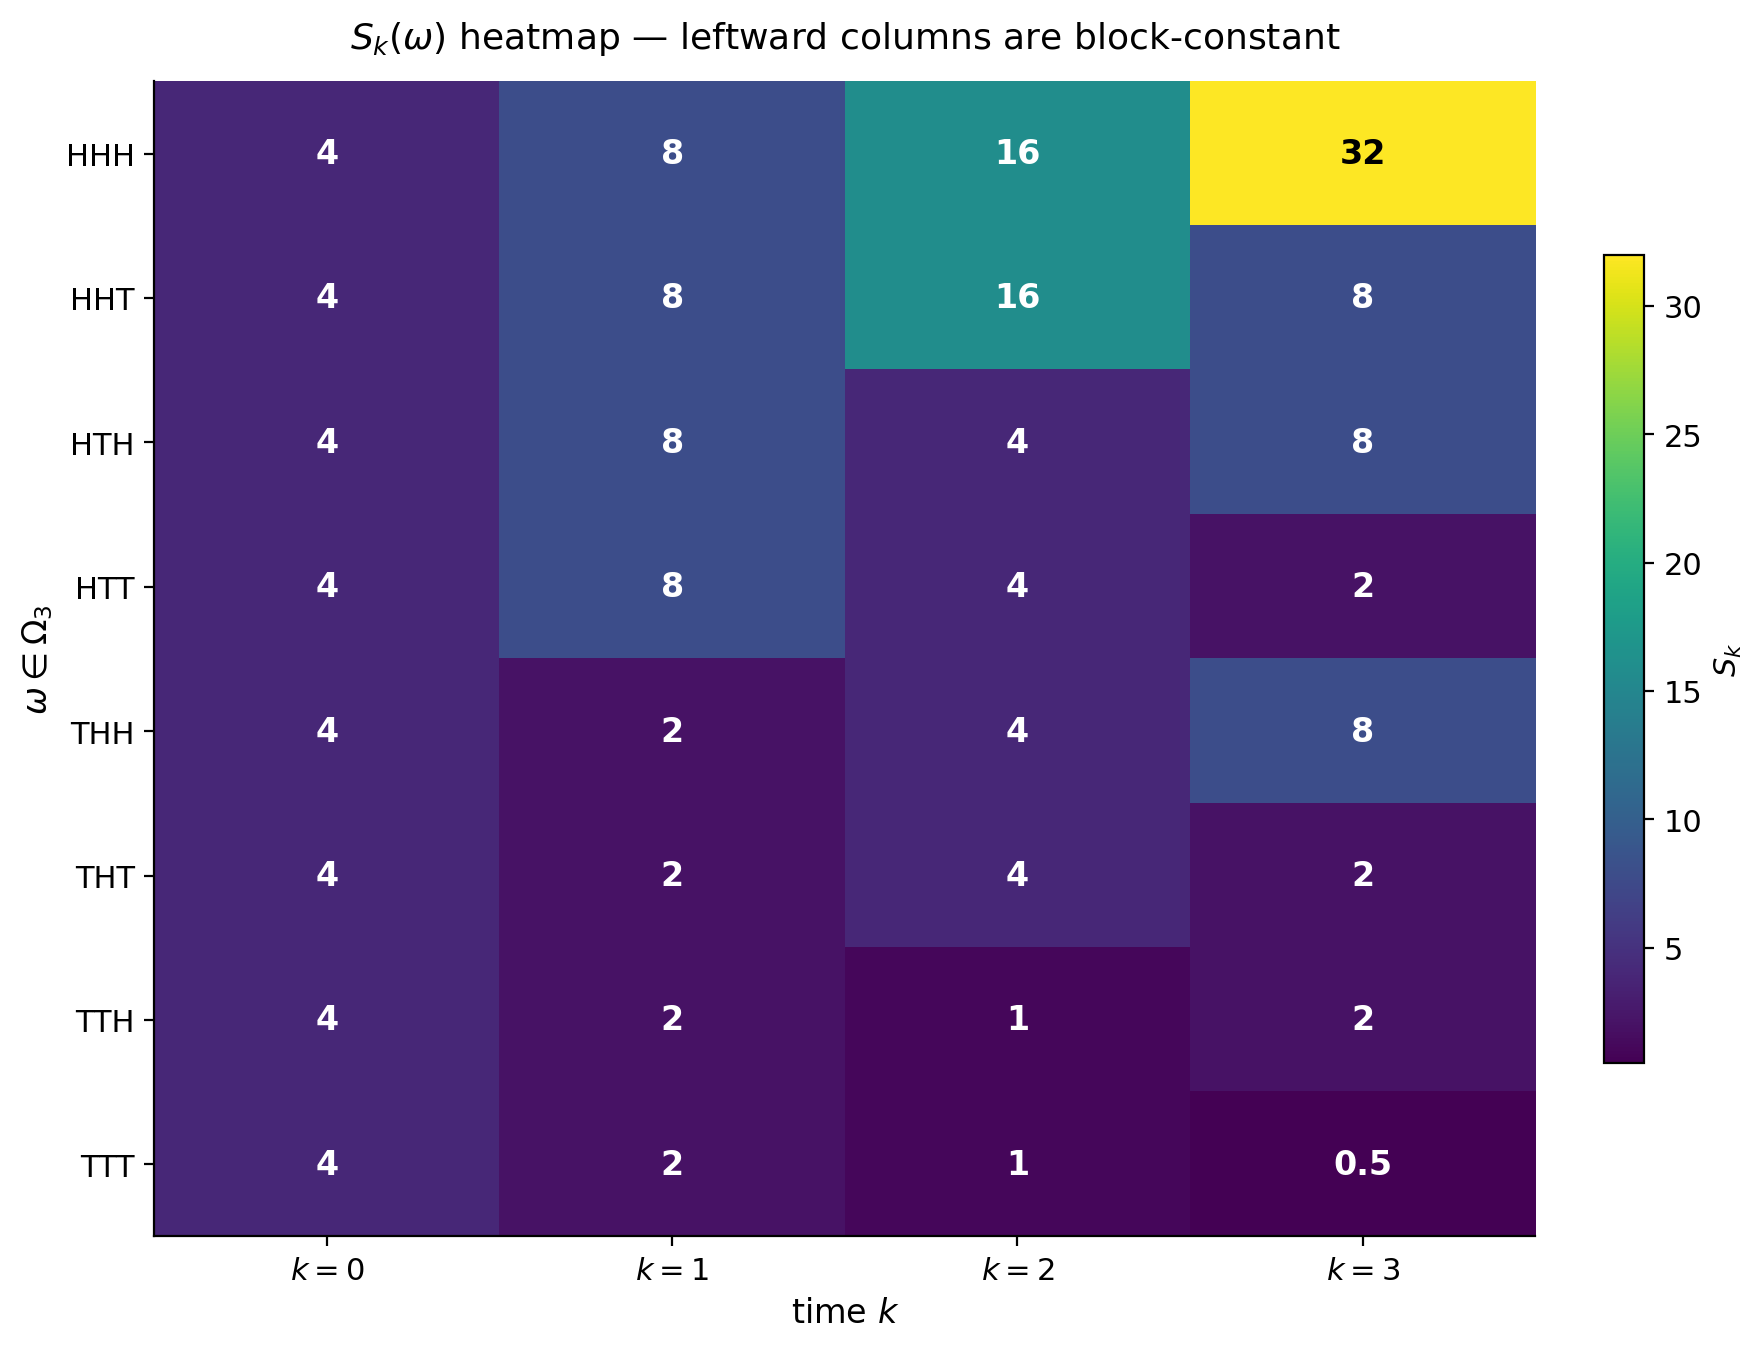
\includegraphics[keepaspectratio]{figures/ch03-Sk-heatmap.png}}
\caption{Heatmap on \(n=3\): rows \(\omega \in \Omega_3\), columns
\(k = 0,1,2,3\), cells coloured by \(S_k(\omega)\). The leftward columns
are \emph{constant on blocks} --- at \(k=0\) the whole column equals 4;
at \(k=1\) the column has two values (block-constant on
\(\mathcal F_1\)); and so on. Constancy increases leftward --- that's
measurability in pictures.}
\end{figure}

\subsection{3.4.3 Table}\label{table-7}

\textbf{Table 3.4.} Path-wise values on \(\Omega_3\). Compare each
column's constancy against the filtration blocks.

{\def\LTcaptype{none} % do not increment counter
\begin{table}[H]
\centering
\begin{tabular}{|l|r|r|r|r|}
\toprule
\(\omega\) & \(S_1\) & \(S_2\) & \(S_3\) & \(M_3 = \max S_k\) \\
\midrule



\(HHH\) & 8 & 16 & 32 & 32 \\
\(HHT\) & 8 & 16 & 8 & 16 \\
\(HTH\) & 8 & 4 & 8 & 8 \\
\(HTT\) & 8 & 4 & 2 & 8 \\
\(THH\) & 2 & 4 & 8 & 8 \\
\(THT\) & 2 & 4 & 2 & 4 \\
\(TTH\) & 2 & 1 & 2 & 4 \\
\(TTT\) & 2 & 1 & 0.5 & 4 \\
\bottomrule
\end{tabular}
\end{table}
}

\(S_1\) is constant on \(\mathcal F_1\)-blocks (top four, bottom four).
\(S_2\) is constant on \(\mathcal F_2\)-blocks (pairs). \(S_3\) and
\(M_3\) vary within \(\mathcal F_2\)-blocks --- they aren't
\(\mathcal F_2\)-measurable.

\begin{center}\rule{0.5\linewidth}{0.5pt}\end{center}

\section{§3.5 Adapted processes}\label{adapted-processes}

\textbf{Punchline.} A stochastic process \(X_0, X_1, \ldots, X_n\) is
\textbf{adapted} to the filtration \(\mathbb F\) if \(X_k\) is
\(\mathcal F_k\)-measurable for every \(k\). In plain English: no
peeking.

\textbf{Intuition.} A trading strategy or a portfolio holding makes
decisions based on what you can see \emph{now}, not what you will see
later. If \(\Delta_k\) is your hedge ratio at time \(k\), the only
information it can use is \(\mathcal F_k\). Adapted = legal = causal.
Non-adapted = clairvoyant.

\subsection{3.5.1 Definitions}\label{definitions-10}

The process \((X_k)_{k=0}^n\) is \textbf{adapted} to \((\mathcal F_k)\)
if \(X_k\) is \(\mathcal F_k\)-measurable for every \(0 \le k \le n\).

For a process built block-by-block on the tree, adapted has the
satisfying visual meaning: at every time \(k\), the value \(X_k\) is the
\emph{same colour} across all leaves in a common \(\mathcal F_k\)-block.
A non-adapted process leaks colour across block boundaries --- you can
see the future.

\subsection{3.5.2 Examples}\label{examples-15}

\textbf{Example 3.5.1 (Stock price \(S\) is adapted).} \(S_k\) depends
on \(\omega_1, \ldots, \omega_k\) alone, hence is
\(\mathcal F_k\)-measurable. ✓

\textbf{Example 3.5.2 (Replicating wealth \(X\) is adapted).} From
Chapter 2, the wealth process satisfies
\(X_{k+1} = \Delta_k S_{k+1} + (1+r)(X_k - \Delta_k S_k)\), with
\(\Delta_k\) chosen \(\mathcal F_k\)-measurable. By induction \(X_k\) is
\(\mathcal F_k\)-measurable.

\textbf{Example 3.5.3 (Running max \(M_k = \max(S_0, \ldots, S_k)\)).}
\(M_k\) depends on \(\omega_1, \ldots, \omega_k\). Adapted. ✓

\textbf{Example 3.5.4 (Look-ahead process \(Y_k = S_{k+1}\)).} \(Y_k\)
depends on \(\omega_1, \ldots, \omega_{k+1}\). Not
\(\mathcal F_k\)-measurable in general, hence not adapted. ✗

\textbf{Example 3.5.5 (Greek-on-tree \(\Delta_k\)).} Chapter 2 built
\(\Delta_k\) by node --- that's \(\mathcal F_k\)-measurable by
construction. Hedges are adapted; clairvoyant hedges would never be
allowed in a real market.

\textbf{Example 3.5.6 (Discounted price
\(\widetilde S_k = S_k / (1+r)^k\)).} Adapted, since \((1+r)^k\) is
deterministic and \(S_k\) is \(\mathcal F_k\)-measurable.

\textbf{Example 3.5.7 (Discounted wealth \(\widetilde X_k\)).} Adapted
by the same argument.

\textbf{Example 3.5.8 (Option intrinsic value \((S_k - K)^+\)).}
Adapted, as a function of \(S_k\).

\textbf{Example 3.5.9 (Time-to-expiry \(n - k\)).} Trivially adapted (in
fact \(\mathcal F_0\)-measurable --- it doesn't depend on \(\omega\) at
all).

\begin{figure}
\centering
\pandocbounded{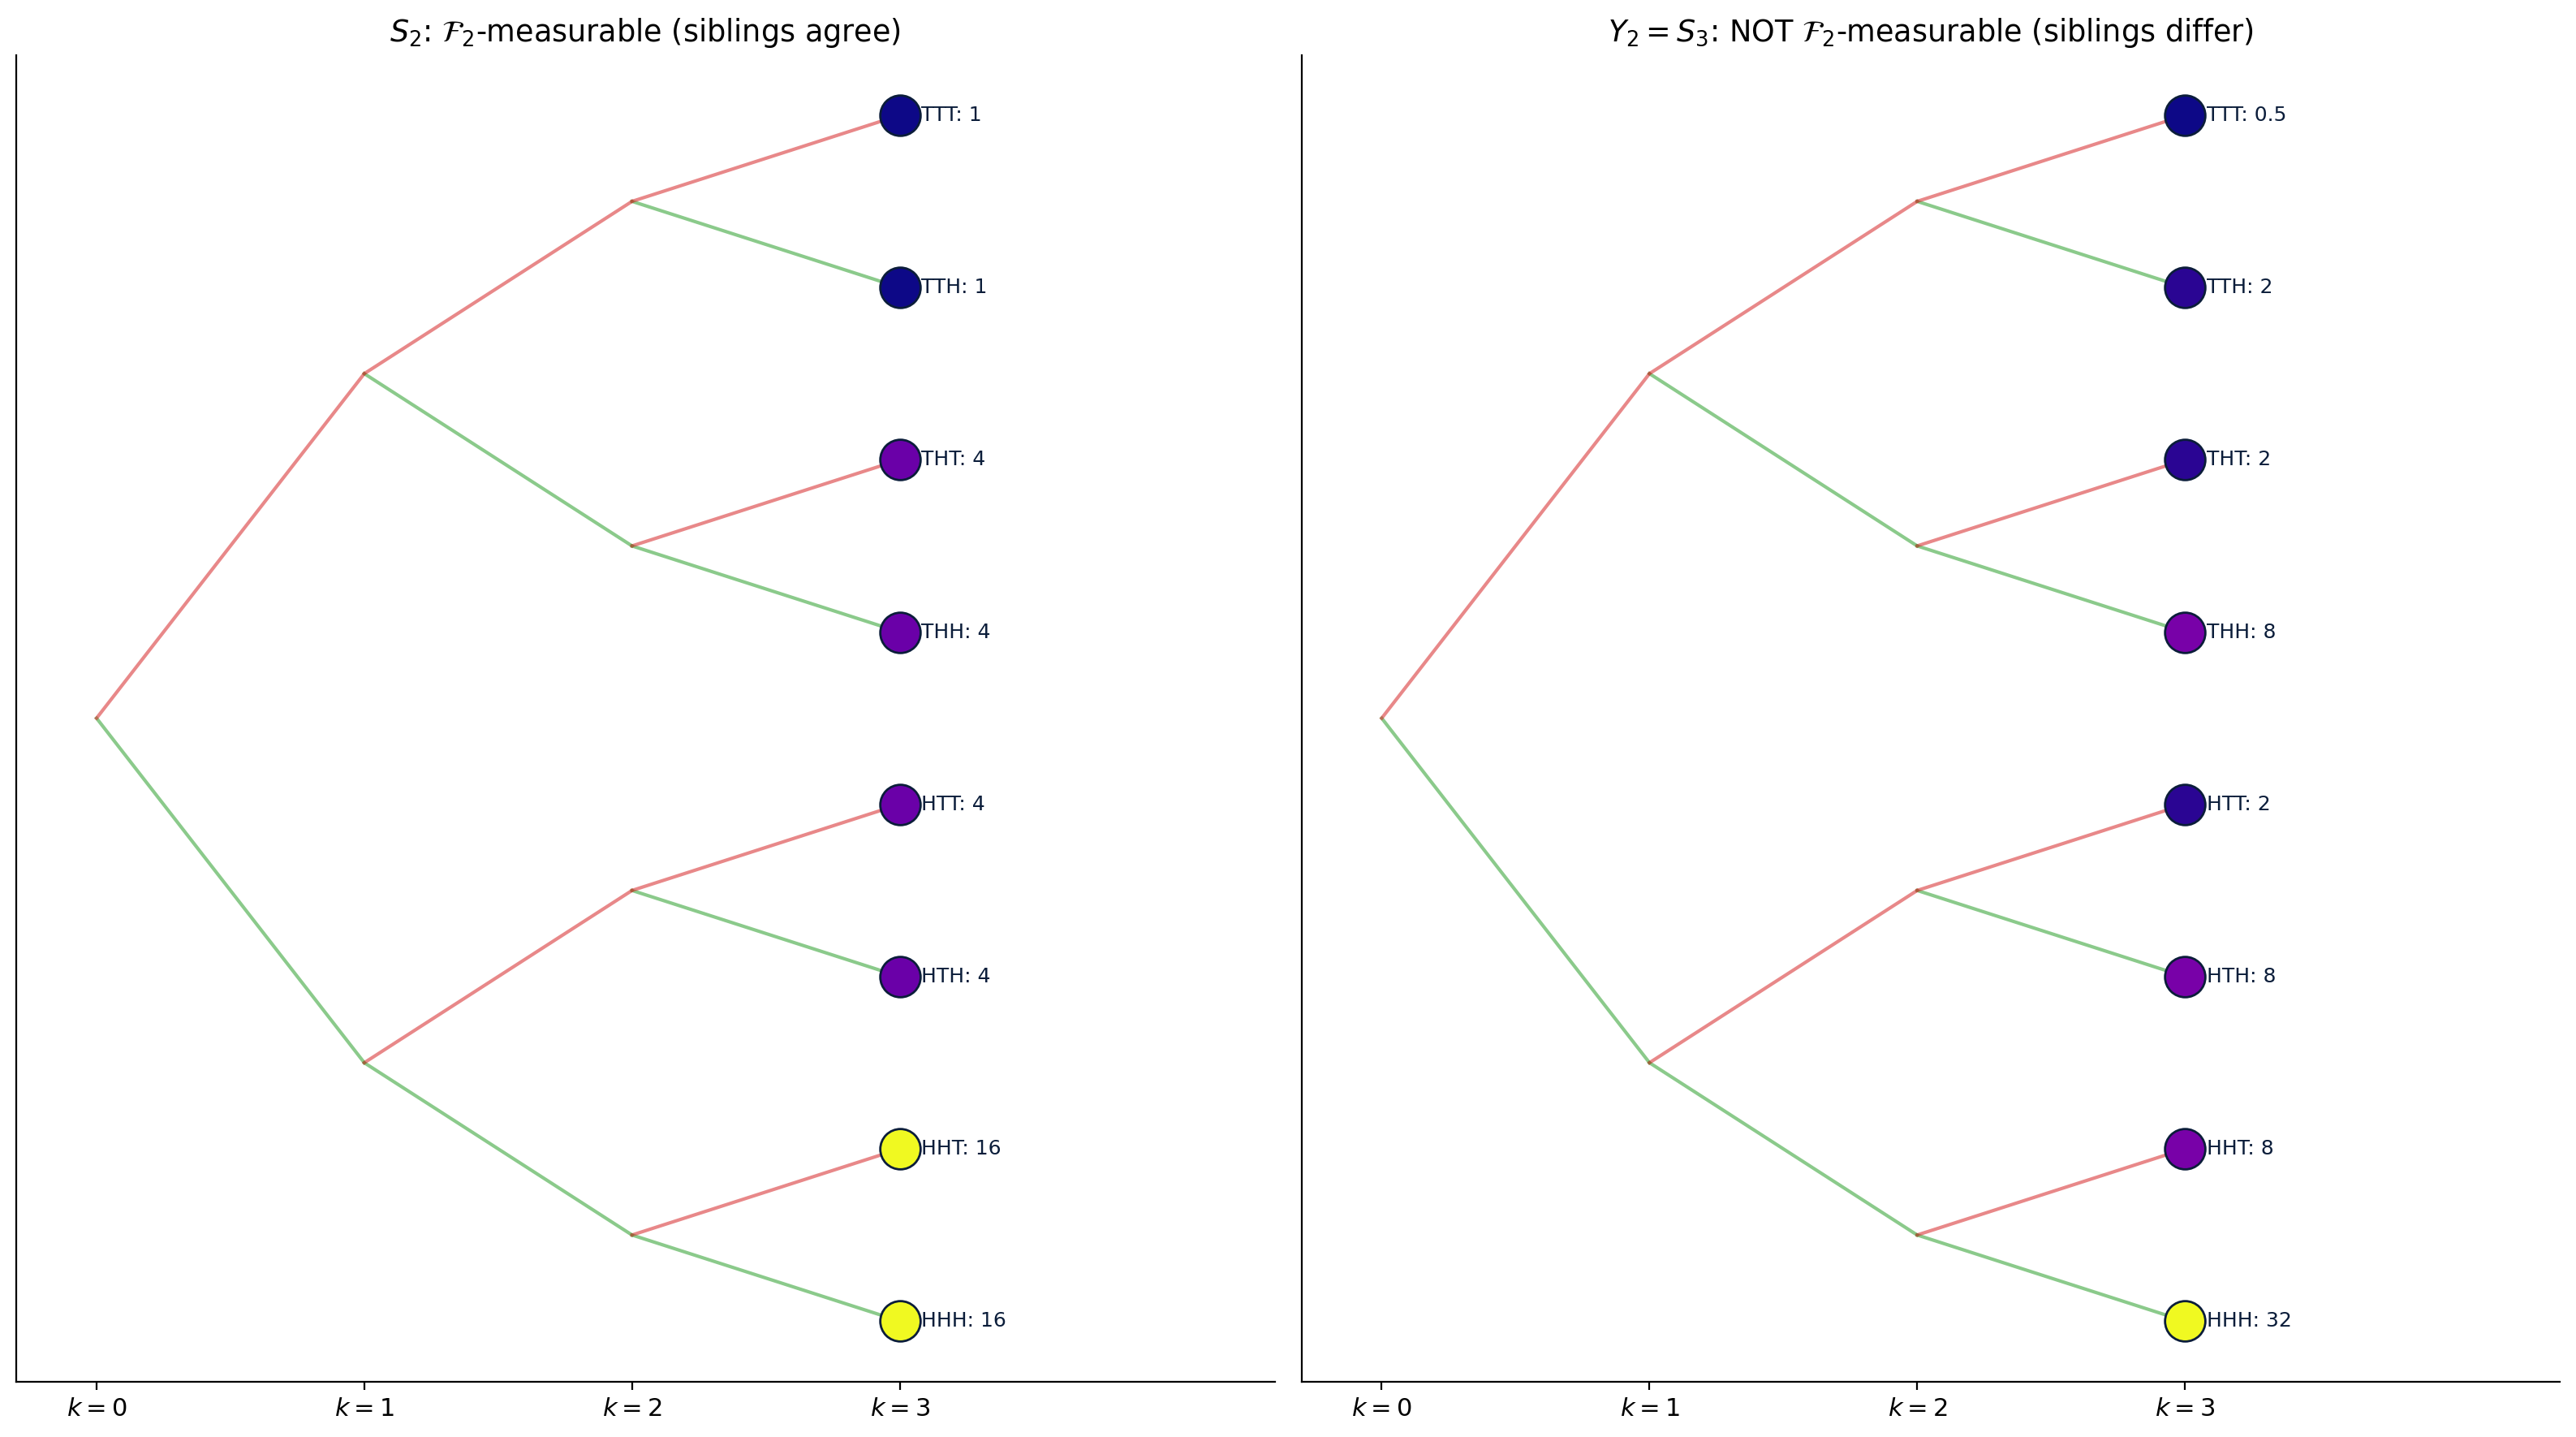
\includegraphics[keepaspectratio]{figures/ch03-adapted-vs-not.png}}
\caption{Two trees side by side. Left: \(S_2\) as a function defined on
all of \(\Omega_3\) --- colours are constant within every
\(\mathcal F_2\)-block (top four leaves vs.~bottom four agree). Right:
\(Y_k = S_{k+1}\) --- colours bleed across \(\mathcal F_k\)-block
boundaries (siblings in a block have different values). The visual
signature of adapted vs not.}
\end{figure}

\subsection{3.5.3 Table}\label{table-8}

\textbf{Table 3.5.} \(\Omega_3\): \(S\) is adapted (each
\(\mathcal F_k\) column is block-constant); \(S_{k+1}\) at time \(k\) is
not (the column varies within blocks).

{\def\LTcaptype{none} % do not increment counter
\begin{table}[H]
\centering
\begin{tabular}{|l|r|r|r|r|r|r|}
\toprule
\(\omega\) & \(S_1\) & \(S_2\) & \(S_3\) & \(Y_0 := S_1\) & \(Y_1 := S_2\) & \(Y_2 := S_3\) \\
\midrule



\(HHH\) & 8 & 16 & 32 & 8 & 16 & 32 \\
\(HHT\) & 8 & 16 & 8 & 8 & 16 & 8 \\
\(HTH\) & 8 & 4 & 8 & 8 & 4 & 8 \\
\(HTT\) & 8 & 4 & 2 & 8 & 4 & 2 \\
\(THH\) & 2 & 4 & 8 & 2 & 4 & 8 \\
\(THT\) & 2 & 4 & 2 & 2 & 4 & 2 \\
\(TTH\) & 2 & 1 & 2 & 2 & 1 & 2 \\
\(TTT\) & 2 & 1 & 0.5 & 2 & 1 & 0.5 \\
\bottomrule
\end{tabular}
\end{table}
}

Column \(Y_0\) is \emph{not} \(\mathcal F_0\)-measurable (it depends on
\(\omega_1\)): a process indexed by \(k=0\) peeking at \(S_1\).

\begin{center}\rule{0.5\linewidth}{0.5pt}\end{center}

\section{§3.6 Conditional expectation
(formal)}\label{conditional-expectation-formal}

\textbf{Punchline.} \(\mathbb E[X \mid \mathcal F_k]\) is the function
on \(\Omega_n\) that, on each \(\mathcal F_k\)-block \(B\), takes the
value equal to the \textbf{block average} of \(X\) --- weighted by the
leaf probabilities within \(B\).

\textbf{Intuition.} ``Expected value of \(X\) given what I know at time
\(k\)'' is the average of \(X\) over all sample points that are still
consistent with my observations. Those sample points are the block of
\(\mathcal F_k\) containing the current \(\omega\). The average uses the
\emph{conditional} probabilities within that block, which under our
independence assumption are just the standard binomial weights over the
remaining \(n-k\) flips.

The result is a \emph{function on \(\Omega_n\)} --- not a single number.
It is itself an \(\mathcal F_k\)-measurable random variable (constant on
each block, by construction).

\subsection{3.6.1 Formal definition}\label{formal-definition}

For \(\omega \in \Omega_n\) let \(B = B(\omega, k)\) denote the
\(\mathcal F_k\)-block containing \(\omega\). Define

\[\mathbb E[X \mid \mathcal F_k](\omega) \;=\; \frac{\sum_{\omega' \in B} X(\omega')\, \mathbb P(\{\omega'\})}{\mathbb P(B)}.\]

The denominator
\(\mathbb P(B) = \sum_{\omega' \in B}\mathbb P(\{\omega'\})\) is
positive (every leaf has positive weight under \(p, 1-p \in (0,1)\)).

Two key properties (both immediate from the formula):

\begin{enumerate}
\def\labelenumi{\arabic{enumi}.}
\tightlist
\item
  \textbf{\(\mathcal F_k\)-measurability}: the right-hand side is
  constant on \(B\), hence the function is constant on every
  \(\mathcal F_k\)-block.
\item
  \textbf{Tower-style averaging consistency}:
  \(\mathbb E[\mathbb E[X \mid \mathcal F_k]] = \mathbb E[X]\) (sum over
  all \(\omega\) and the block factor telescopes).
\end{enumerate}

Under independence of the flips, the conditional probability of an
unobserved tail \(\omega_{k+1}\ldots\omega_n\) given the observed prefix
is just the product weight of the tail. In particular, \emph{for an
\(\mathcal F_k\)-measurable random variable} \(Y\),
\(\mathbb E[Y \mid \mathcal F_k] = Y\) (block-average of a constant is
the constant).

\subsection{3.6.2 Examples}\label{examples-16}

\textbf{Example 3.6.1 (\(\tilde{\mathbb E}[S_3 \mid \mathcal F_2]\) on
Toy, all 4 blocks).} Conditional on the prefix being known, \(\omega_3\)
is the only unknown, with \(\tilde p = 1/2\) for \(H\) and \(1/2\) for
\(T\). Each leaf \(S_3 = u\,S_2\) or \(d\,S_2\) with \(u=2, d=0.5\):

\begin{itemize}
\tightlist
\item
  Block \(A_{HH}\) (\(S_2 = 16\)): leaves \(HHH, HHT\) with
  \(S_3 \in \{32, 8\}\). Average: \((32+8)/2 = 20\).
\item
  Block \(A_{HT}\) (\(S_2 = 4\)): leaves \(HTH, HTT\) with
  \(S_3 \in \{8, 2\}\). Average: \(5\).
\item
  Block \(A_{TH}\) (\(S_2 = 4\)): leaves \(THH, THT\) with
  \(S_3 \in \{8, 2\}\). Average: \(5\).
\item
  Block \(A_{TT}\) (\(S_2 = 1\)): leaves \(TTH, TTT\) with
  \(S_3 \in \{2, 0.5\}\). Average: \(1.25\).
\end{itemize}

\textbf{Example 3.6.2 (Cross-check with \((1+r)\, S_2\)).} Toy has
\(r=0.25\), so \((1+r)S_2 = 1.25 S_2\). Block by block:
\(1.25\cdot 16=20\), \(1.25\cdot 4=5\), \(1.25\cdot 4=5\),
\(1.25\cdot 1=1.25\) --- match the four averages above exactly. So
\(\tilde{\mathbb E}[S_3 \mid \mathcal F_2] = (1+r)\, S_2\) everywhere,
confirming the one-step risk-neutral law. \emph{Equivalently, the
discounted price \(\widetilde S_k = S_k/(1+r)^k\) is a martingale under
\(\tilde{\mathbb P}\).}

\textbf{Example 3.6.3 (Real-world drift differs).} With \(p = 0.6\):
\(\mathbb E[S_3 \mid \mathcal F_2] = (0.6\cdot 2 + 0.4 \cdot 0.5)\cdot S_2 = 1.4\cdot S_2\).
On \(A_{HH}\): \(1.4 \cdot 16 = 22.4\). (Check:
\(0.6 \cdot 32 + 0.4 \cdot 8 = 19.2 + 3.2 = 22.4\). ✓) The factor
\(1.4 > 1+r = 1.25\) means real-world expected price grows faster than
the risk-free rate --- exactly the \emph{equity risk premium}.

\textbf{Example 3.6.4 (\(\tilde{\mathbb E}[S_2 \mid \mathcal F_1]\) on
Toy).} Two blocks:

\begin{itemize}
\tightlist
\item
  \(A_H\) (\(S_1 = 8\)):
  \(\tilde{\mathbb E}[S_2 \mid A_H] = 0.5 \cdot 16 + 0.5 \cdot 4 = 10 = 1.25 \cdot 8\).
  ✓
\item
  \(A_T\) (\(S_1 = 2\)):
  \(\tilde{\mathbb E}[S_2 \mid A_T] = 0.5 \cdot 4 + 0.5 \cdot 1 = 2.5 = 1.25 \cdot 2\).
  ✓
\end{itemize}

\textbf{Example 3.6.5 (Realistic,
\(\tilde{\mathbb E}[(S_3 - 95)^+ \mid S_2 = 121]\)).} Realistic params:
\(u=1.10, d=0.90, r=0.02, \tilde p = 0.6\). If \(S_2 = 121\) (path
\(HH\)), then conditional on this block,
\(S_3 \in \{121 \cdot 1.10 = 133.10,\; 121 \cdot 0.90 = 108.90\}\) with
\(\tilde p, 1-\tilde p\). Payoff \((S_3 - 95)^+ \in \{38.10, 13.90\}\).
Conditional expectation:
\(0.6 \cdot 38.10 + 0.4 \cdot 13.90 = 22.86 + 5.56 = 28.42\). So
\(\tilde{\mathbb E}[(S_3 - 95)^+ \mid S_2 = 121] = 28.42\).

\textbf{Example 3.6.6
(\(\tilde{\mathbb E}[\mathbf 1_{\{S_3 = 8\}} \mid \mathcal F_2]\) on
Toy).} Block by block:

\begin{itemize}
\tightlist
\item
  \(A_{HH}\): \(S_3 \in \{32, 8\}\). Indicator = \(\{0,1\}\) with
  \(\tilde p, 1-\tilde p\). Avg \(= 1/2\).
\item
  \(A_{HT}\): \(S_3 \in \{8, 2\}\). Indicator \(= \{1, 0\}\). Avg
  \(= 1/2\).
\item
  \(A_{TH}\): \(S_3 \in \{8, 2\}\). Indicator \(= \{1, 0\}\). Avg
  \(= 1/2\).
\item
  \(A_{TT}\): \(S_3 \in \{2, 0.5\}\). Indicator \(= \{0, 0\}\). Avg
  \(= 0\).
\end{itemize}

Conditional probability of hitting \(S_3 = 8\) given \(\mathcal F_2\) is
\(1/2\) on the first three blocks and \(0\) on the fourth.

\textbf{Example 3.6.7 (Pull out what's known).} \(S_2\) is
\(\mathcal F_2\)-measurable. So
\(\tilde{\mathbb E}[S_2 \cdot S_3 \mid \mathcal F_2] = S_2 \cdot \tilde{\mathbb E}[S_3 \mid \mathcal F_2] = S_2 \cdot 1.25 S_2 = 1.25 S_2^2\).
On \(A_{HH}\): \(1.25 \cdot 256 = 320\).

\textbf{Example 3.6.8 (Independence: \(\omega_3\) given
\(\mathcal F_2\)).} Since flips are independent,
\(\tilde{\mathbb E}[\mathbf 1_{\{\omega_3 = H\}} \mid \mathcal F_2] = \tilde p = 0.5\)
on every block --- a \emph{constant function}, even though it could in
principle vary block-to-block.

\begin{figure}
\centering
\pandocbounded{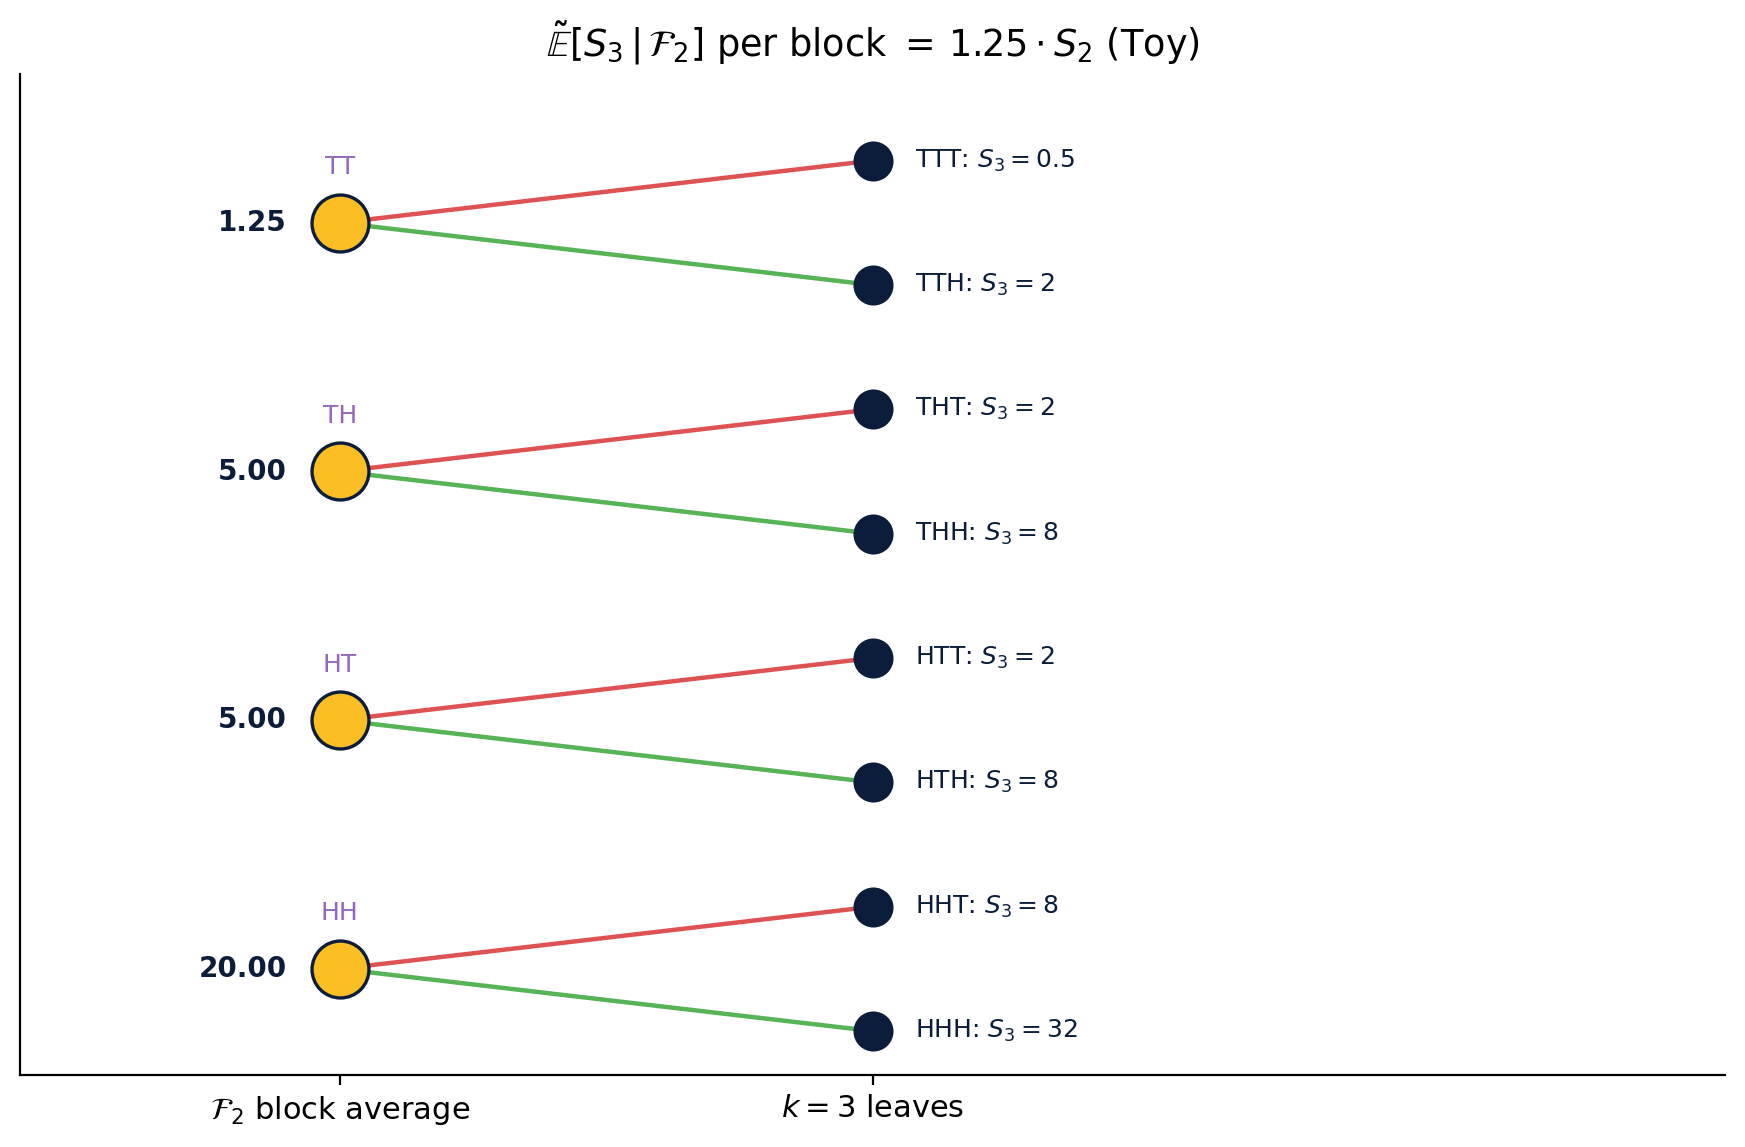
\includegraphics[keepaspectratio]{figures/ch03-block-average-tree.png}}
\caption{Tree on \(\Omega_3\) with each \(\mathcal F_2\)-block replaced
by a single node carrying the block's \(\tilde{\mathbb P}\)-average of
\(S_3\). The leaves at the right show the four pairs; the centre column
shows the four averages 20, 5, 5, 1.25. The implicit cross-check is that
each block average equals \(1.25 \cdot S_2\).}
\end{figure}

\begin{figure}
\centering
\pandocbounded{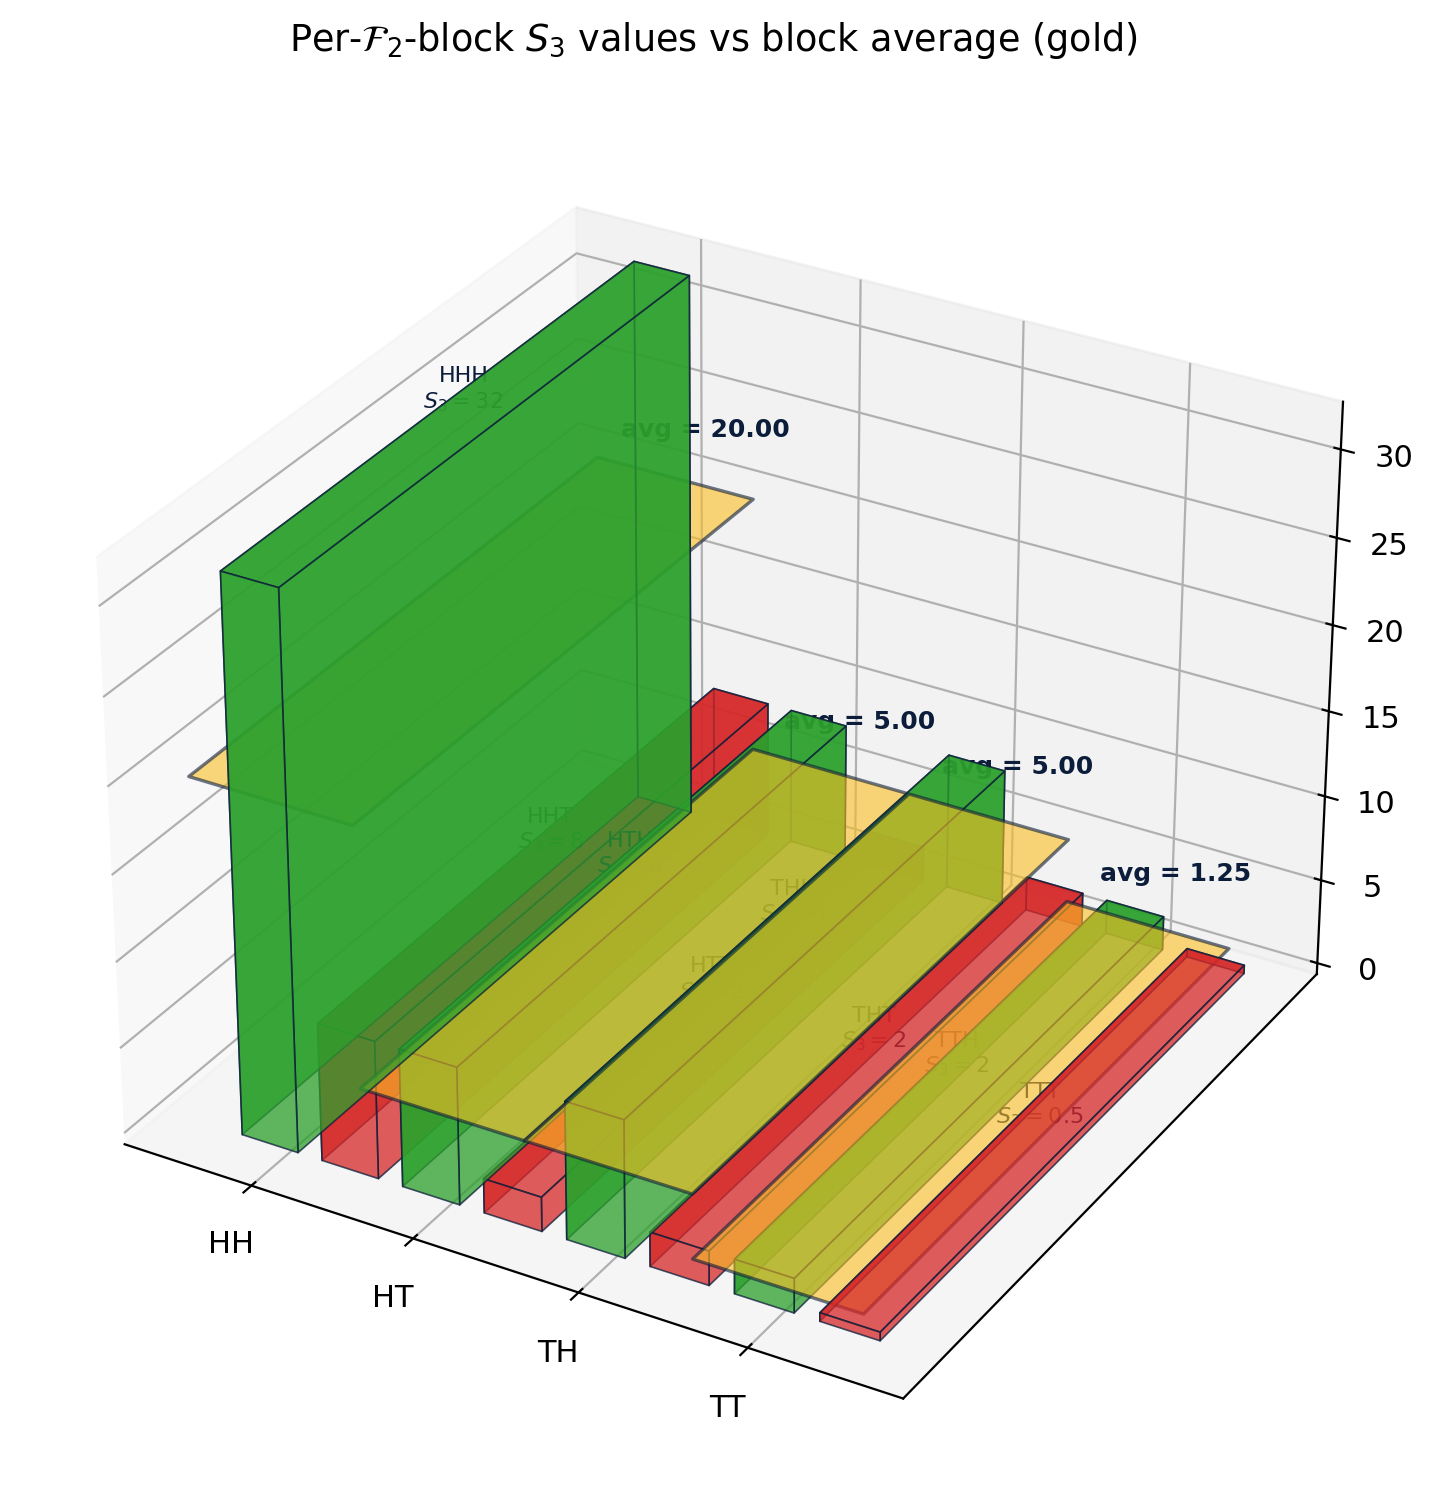
\includegraphics[keepaspectratio]{figures/ch03-block-avg-3d.png}}
\caption{3-D bars: \(x\) axis indexes \(\mathcal F_2\)-blocks (HH, HT,
TH, TT). For each block we plot two bars at \(z = S_3\) for the two
leaves, and overlay a horizontal segment at the block average. Bars
cluster around the average --- the conditional expectation as the ``best
block-constant approximation''.}
\end{figure}

\subsection{3.6.3 Table}\label{table-9}

\textbf{Table 3.6.} Conditional expectation worksheet for
\(\tilde{\mathbb E}[S_3 \mid \mathcal F_2]\) on Toy
(\(\tilde p = 0.5\)).

{\def\LTcaptype{none} % do not increment counter
\begin{table}[H]
\centering
\begin{tabular}{|l|l|l|r|r|}
\toprule
Block & leaves & \(S_3\) values & block average & \(1.25 \cdot S_2\) check \\
\midrule



\(A_{HH}\) & \(HHH, HHT\) & \(32, 8\) & \(20\) & \(1.25 \cdot 16 = 20\)
✓ \\
\(A_{HT}\) & \(HTH, HTT\) & \(8, 2\) & \(5\) & \(1.25 \cdot 4 = 5\) ✓ \\
\(A_{TH}\) & \(THH, THT\) & \(8, 2\) & \(5\) & \(1.25 \cdot 4 = 5\) ✓ \\
\(A_{TT}\) & \(TTH, TTT\) & \(2, 0.5\) & \(1.25\) &
\(1.25 \cdot 1 = 1.25\) ✓ \\
\bottomrule
\end{tabular}
\end{table}
}

\begin{center}\rule{0.5\linewidth}{0.5pt}\end{center}

\section{§3.7 Tower property revisited}\label{tower-property-revisited}

\textbf{Punchline.} \emph{Average then average = average once.}
Formally: for \(k \le m\),

\[\mathbb E[\,\mathbb E[X \mid \mathcal F_m]\,\mid \mathcal F_k\,] = \mathbb E[X \mid \mathcal F_k].\]

Also in the simplest form (\(k = 0\)):
\(\mathbb E[\mathbb E[X \mid \mathcal F_m]] = \mathbb E[X]\).

\textbf{Intuition.} A fine block-average then a coarse block-average is
just the coarse block-average directly. The ``tower'' name comes from
drawing nested partitions stacked vertically: averaging at the finer
level then re-averaging at the coarser is the same as a single trip down
the stack.

\subsection{3.7.1 Three workhorse
identities}\label{three-workhorse-identities}

(All under any measure; they only use the block-average structure.)

\begin{enumerate}
\def\labelenumi{\arabic{enumi}.}
\tightlist
\item
  \textbf{Tower}:
  \(\mathbb E[\mathbb E[X\mid\mathcal F_m]\mid\mathcal F_k] = \mathbb E[X\mid\mathcal F_k]\)
  for \(k \le m\).
\item
  \textbf{Pull-out}: if \(Y\) is \(\mathcal F_k\)-measurable, then
  \(\mathbb E[YX \mid \mathcal F_k] = Y\,\mathbb E[X\mid\mathcal F_k]\).
\item
  \textbf{Independence collapse}: if \(X\) is \emph{independent} of
  \(\mathcal F_k\), then \(\mathbb E[X\mid\mathcal F_k] = \mathbb E[X]\)
  (a constant).
\end{enumerate}

These three combined are nearly the whole calculation kit for the rest
of the book.

\subsection{3.7.2 Examples}\label{examples-17}

\textbf{Example 3.7.1 (Numeric tower check on Toy, \(X = S_3\)).} From
§3.6.2 Example 3.6.1, \(\tilde{\mathbb E}[S_3 \mid \mathcal F_2]\) is
the function on \(\Omega_3\) taking values
\(\{20, 20, 5, 5, 5, 5, 1.25, 1.25\}\) on the eight leaves (each block
of two has the common block average). Now compute the \emph{next}
average, to \(\mathcal F_1\):

\begin{itemize}
\tightlist
\item
  \(A_H\) contains the leaves of \(A_{HH}, A_{HT}\). Their
  inner-conditional values are \(\{20,20,5,5\}\). Average (with
  \(\tilde p = 0.5\)): each leaf weight \(1/4\) within \(A_H\), so
  \((20+20+5+5)/4 = 12.5\).
\item
  \(A_T\) contains the leaves of \(A_{TH}, A_{TT}\). Inner-conditional
  values \(\{5,5,1.25,1.25\}\). Average: \((5+5+1.25+1.25)/4 = 3.125\).
\end{itemize}

Compare to \(\tilde{\mathbb E}[S_3 \mid \mathcal F_1]\) direct: \(A_H\)
has \(S_3 \in \{32, 8, 8, 2\}\), avg \((32+8+8+2)/4 = 12.5\). ✓ \(A_T\)
has \(S_3 \in \{8, 2, 2, 0.5\}\), avg \(3.125\). ✓ Tower works.

\textbf{Example 3.7.2 (Pull-out,
\(\tilde{\mathbb E}[S_1 \cdot S_3 \mid \mathcal F_1]\)).} \(S_1\) is
\(\mathcal F_1\)-measurable. Pull-out gives
\(\tilde{\mathbb E}[S_1 S_3 \mid \mathcal F_1] = S_1 \tilde{\mathbb E}[S_3 \mid \mathcal F_1]\).
On \(A_H\) that's \(8 \cdot 12.5 = 100\).

\textbf{Example 3.7.3 (Independence collapse,
\(\omega_3 \perp \mathcal F_2\)).}
\(\tilde{\mathbb E}[\mathbf 1_{\{\omega_3 = H\}} \mid \mathcal F_2] = \tilde p = 0.5\).
The third toss is independent of the first two, so conditioning on
\(\mathcal F_2\) tells you nothing about \(\omega_3\).

\textbf{Example 3.7.4 (Identity verified directly).}
\(\tilde{\mathbb E}[\mathbf 1_{\{\omega_3 = H\}}] = 0.5\)
unconditionally. Tower says
\(\tilde{\mathbb E}[\tilde{\mathbb E}[\mathbf 1_{\{\omega_3=H\}} \mid \mathcal F_2]] = \tilde{\mathbb E}[0.5] = 0.5\).
✓

\textbf{Example 3.7.5 (Two-step risk-neutral expected gross return).}
\(\tilde{\mathbb E}[S_3 / S_1 \mid \mathcal F_1] = (1+r)^2\) since
\(\tilde{\mathbb E}[S_3 / S_1 \mid \mathcal F_1] = \tilde{\mathbb E}[\,(\tilde{\mathbb E}[S_3 / S_2 \mid \mathcal F_2]) \cdot S_2 / S_1 \mid \mathcal F_1] = \tilde{\mathbb E}[(1+r)\,S_2 / S_1 \mid \mathcal F_1] = (1+r)^2\).
On Toy, \((1+r)^2 = 1.5625\). Cross-check on \(A_H\): leaves
\(HHH, HHT, HTH, HTT\) have
\(S_3/S_1 = \{32/8, 8/8, 8/8, 2/8\} = \{4, 1, 1, 0.25\}\), avg
\(6.25/4 = 1.5625\). ✓

\textbf{Example 3.7.6 (Realistic).} Same identity, \(\tilde p = 0.6\):
\(\tilde{\mathbb E}[S_3 / S_1 \mid \mathcal F_1] = 1.02^2 = 1.0404\).

\textbf{Example 3.7.7 (Multi-step pull-out).} For deterministic \(a_k\):
\(\tilde{\mathbb E}[a_k S_k \mid \mathcal F_m] = a_k \tilde{\mathbb E}[S_k \mid \mathcal F_m]\).
Useful when discounting.

\textbf{Example 3.7.8 (Tower for option price recursion).} Let
\(V_k = \tilde{\mathbb E}[V_n / (1+r)^{n-k} \mid \mathcal F_k]\) be the
time-\(k\) price of a European option with payoff \(V_n\). Then
\(V_k = \tilde{\mathbb E}[V_{k+1} / (1+r) \mid \mathcal F_k]\) --- this
is the \emph{tower property in disguise}. It is exactly the backward
induction of Chapter 2.

\begin{figure}
\centering
\pandocbounded{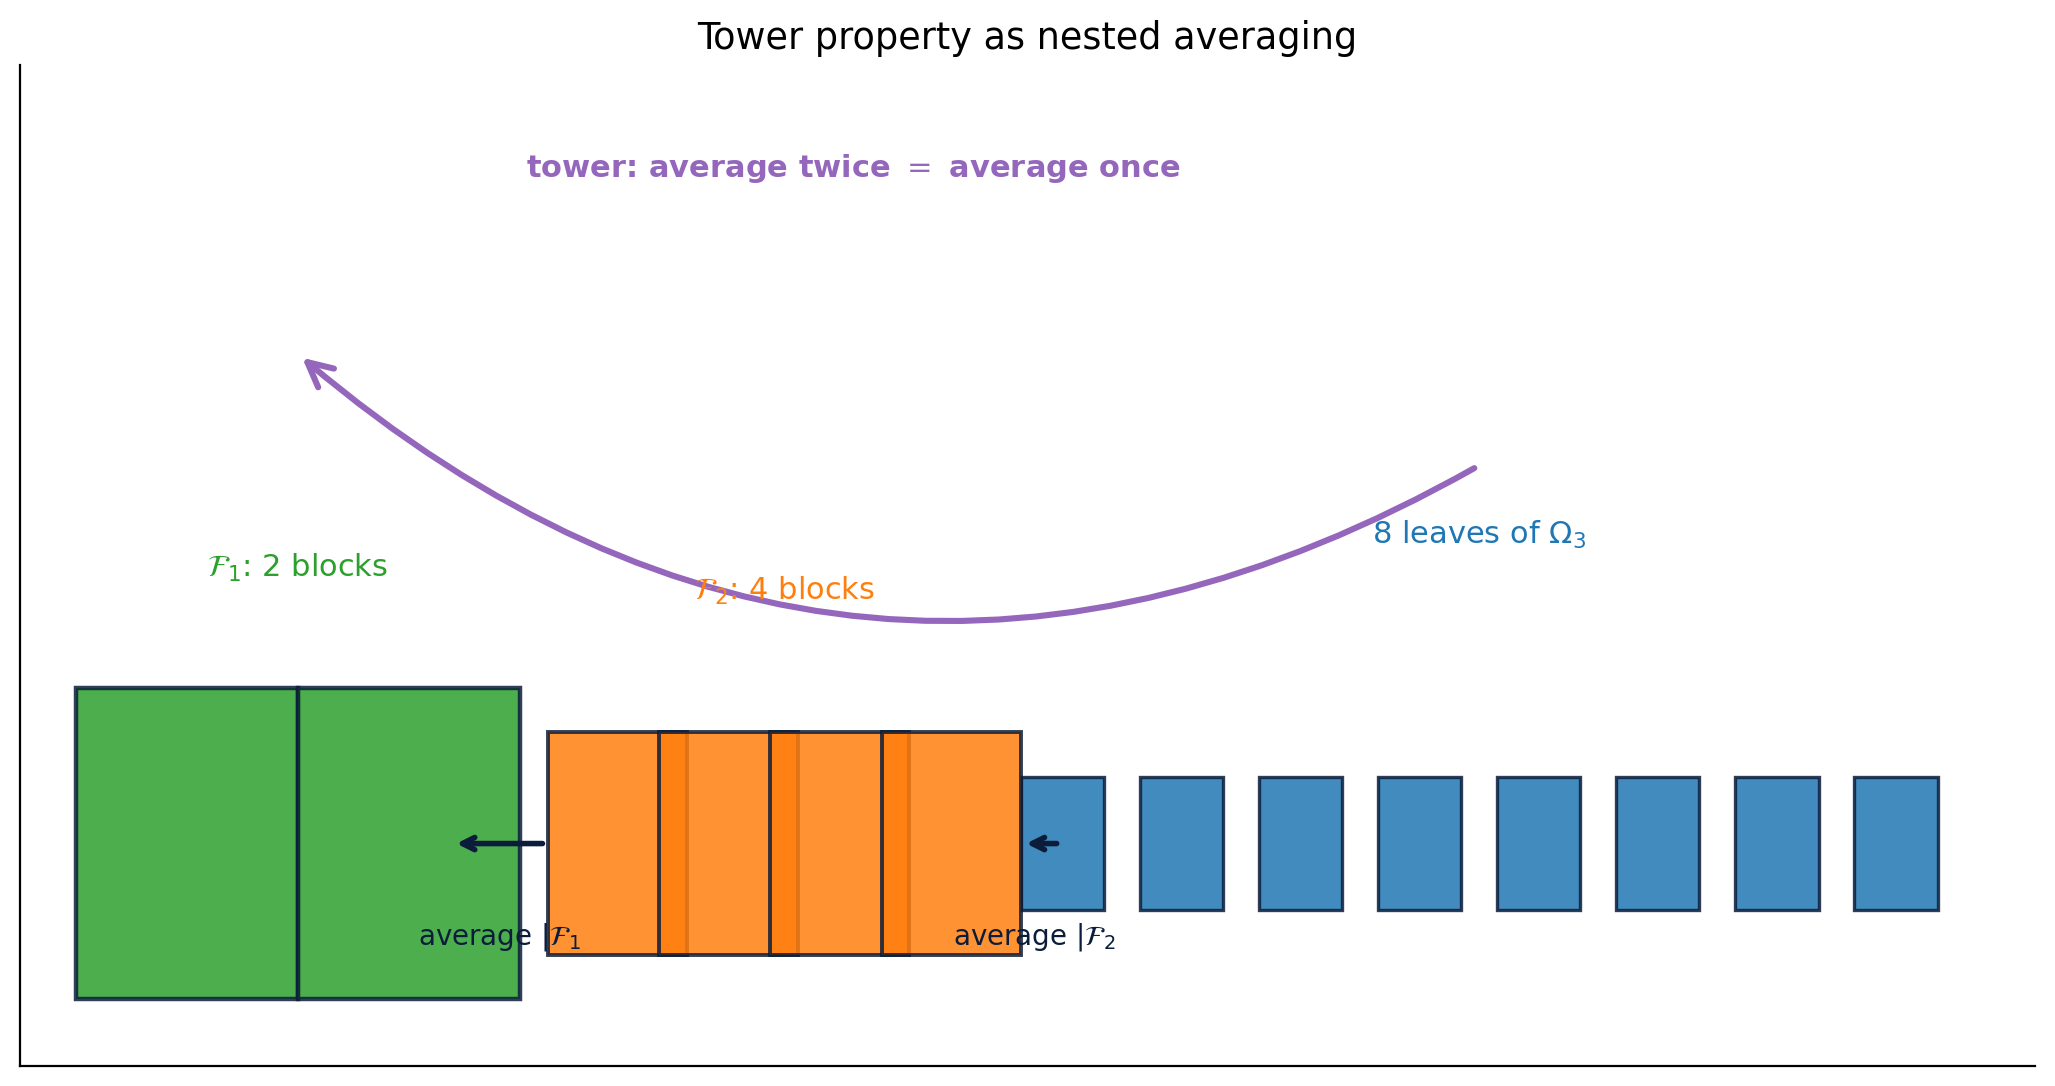
\includegraphics[keepaspectratio]{figures/ch03-tower-cartoon.png}}
\caption{Cartoon nested squares: at left, the leaves of \(\Omega_3\) are
8 small blue squares. They are gathered into 4 orange squares
(\(\mathcal F_2\)-blocks), which are gathered into 2 green squares
(\(\mathcal F_1\)-blocks). The arrow says ``average twice \(=\) average
once'' by routing through the orange or skipping straight to green.}
\end{figure}

\subsection{3.7.3 Table}\label{table-10}

\textbf{Table 3.7.} The three identities, applied to \(X = S_3\) with
\(\tilde p = 0.5\).

{\def\LTcaptype{none} % do not increment counter
\begin{table}[H]
\centering
\begin{tabular}{|l|l|}
\toprule
Identity & Numeric result \\
\midrule



Tower & \(12.5\) on \(A_H\), \(3.125\) on \(A_T\) \\
Pull-out & \(8 \cdot 12.5 = 100\) on \(A_H\) \\
Independence & \(0.5\) on every block \\
\bottomrule
\end{tabular}
\end{table}
}

Identity statements (full form):

\begin{enumerate}
\def\labelenumi{\arabic{enumi}.}
\tightlist
\item
  \textbf{Tower:}
  \(\tilde{\mathbb E}[\tilde{\mathbb E}[S_3 \mid \mathcal F_2] \mid \mathcal F_1] = \tilde{\mathbb E}[S_3 \mid \mathcal F_1]\).
\item
  \textbf{Pull-out:}
  \(\tilde{\mathbb E}[S_1 S_3 \mid \mathcal F_1] = S_1\, \tilde{\mathbb E}[S_3 \mid \mathcal F_1]\).
\item
  \textbf{Independence:}
  \(\tilde{\mathbb E}[\mathbf 1_{\omega_3 = H} \mid \mathcal F_2] = \tilde p\).
\end{enumerate}

\begin{center}\rule{0.5\linewidth}{0.5pt}\end{center}

\section{§3.8 Martingales in discrete
time}\label{martingales-in-discrete-time}

\textbf{Punchline.} A \emph{fair process}:
\(\mathbb E[M_{k+1} \mid \mathcal F_k] = M_k\). \emph{Theorem}: under
the risk-neutral measure \(\tilde{\mathbb P}\), the discounted price
\(\widetilde M_k := S_k / (1+r)^k\) is a martingale.

\textbf{Intuition.} ``Martingale'' originally meant a fair gambling
strategy --- your expected wealth doesn't grow, doesn't shrink. In our
setting, \emph{the entire point} of \(\tilde p\) in Chapter 1 was that
it makes discounted price expected-flat. We are now confirming that
property algebraically, on every block, at every \(k\).

The risk-neutral measure is sometimes called the \emph{martingale
measure} for exactly this reason: it's the measure under which the
discounted underlying is a martingale.

\subsection{3.8.1 Definitions}\label{definitions-11}

An adapted process \((M_k)_{k=0}^n\) is a \textbf{martingale} with
respect to \((\mathcal F_k)\) under measure \(\mathbb P\) if

\[\mathbb E[M_{k+1} \mid \mathcal F_k] = M_k \quad\text{for every } 0 \le k \le n-1.\]

A \textbf{submartingale} has \(\ge\) instead of \(=\); a
\textbf{supermartingale} has \(\le\). The differences capture drift:
submartingale drifts up on average, supermartingale drifts down.

\subsection{3.8.2 The central theorem}\label{the-central-theorem}

\textbf{Theorem (discounted stock is risk-neutral martingale).} Under
\(\tilde{\mathbb P}\) with \(\tilde p = \frac{(1+r) - d}{u - d}\),

\[\tilde{\mathbb E}\!\left[\,\frac{S_{k+1}}{(1+r)^{k+1}}\,\Big|\,\mathcal F_k\right] \;=\; \frac{S_k}{(1+r)^k}.\]

\emph{Proof (one step).} Conditional on \(\mathcal F_k\), \(S_{k+1}\) is
either \(u S_k\) (prob \(\tilde p\)) or \(d S_k\) (prob \(1-\tilde p\)).
So
\[\tilde{\mathbb E}[S_{k+1} \mid \mathcal F_k] = (\tilde p\,u + (1-\tilde p)\,d)\, S_k = (1+r)\, S_k\]
by the definition of \(\tilde p\). Divide both sides by \((1+r)^{k+1}\).
∎

\subsection{3.8.3 Examples}\label{examples-18}

\textbf{Example 3.8.1 (Verify on Toy, all \(\mathcal F_2\)-blocks).}
Compute \(\widetilde M_k = S_k / (1+r)^k\):

\begin{itemize}
\tightlist
\item
  \(\widetilde M_0 = 4 / 1 = 4\).
\item
  \(\widetilde M_1(H) = 8 / 1.25 = 6.4\);
  \(\widetilde M_1(T) = 2 / 1.25 = 1.6\).
\item
  \(\widetilde M_2(HH) = 16 / 1.5625 = 10.24\);
  \(\widetilde M_2(HT) = \widetilde M_2(TH) = 4 / 1.5625 = 2.56\);
  \(\widetilde M_2(TT) = 1 / 1.5625 = 0.64\).
\item
  \(\widetilde M_3(HHH) = 32 / 1.953125 = 16.384\), etc.
\end{itemize}

Check \(\tilde{\mathbb E}[\widetilde M_3 \mid \mathcal F_2]\) on
\(A_{HH}\): \((0.5)(16.384) + (0.5)(\widetilde M_3(HHT))\).
\(\widetilde M_3(HHT) = 8/1.953125 = 4.096\). Avg
\(= (16.384 + 4.096)/2 = 10.24 = \widetilde M_2(HH)\). ✓

\textbf{Example 3.8.2 (\(A_{HT}\)).}
\(\widetilde M_3(HTH) = 8/1.953125 = 4.096\);
\(\widetilde M_3(HTT) = 2/1.953125 = 1.024\). Avg
\(= 2.56 = \widetilde M_2(HT)\). ✓

\textbf{Example 3.8.3 (\(A_{TT}\)).} \(\widetilde M_3(TTH) = 1.024\);
\(\widetilde M_3(TTT) = 0.5/1.953125 = 0.256\). Avg
\(= 0.64 = \widetilde M_2(TT)\). ✓

\textbf{Example 3.8.4 (Realistic, \(n=1\)).} \(\tilde p = 0.6\).
\(\tilde{\mathbb E}[\widetilde M_1] = 0.6 \cdot 110/1.02 + 0.4 \cdot 90/1.02 = (66 + 36)/1.02 = 102/1.02 = 100 = \widetilde M_0\).
✓

\textbf{Example 3.8.5 (Realistic, \(n=2\)).} From the block
\(\{S_1 = 110\}\):
\(\tilde{\mathbb E}[\widetilde M_2 \mid \mathcal F_1] = 0.6 \cdot 121/1.0404 + 0.4 \cdot 99/1.0404 = (72.6 + 39.6)/1.0404 = 112.2/1.0404 = 107.84\).
And \(\widetilde M_1(H) = 110/1.02 = 107.84\). ✓

\textbf{Example 3.8.6 (Sub-martingale under real-world).} With
\(p = 0.6\) (real-world) on Toy:
\(\mathbb E[S_{k+1}/(1+r)^{k+1} \mid \mathcal F_k] = (pu + (1-p)d)/(1+r) \cdot \widetilde M_k = (0.6 \cdot 2 + 0.4 \cdot 0.5)/1.25 \cdot \widetilde M_k = 1.4/1.25 \cdot \widetilde M_k = 1.12 \widetilde M_k > \widetilde M_k\).
So \(\widetilde M\) is a \emph{strict sub-martingale} under
\(\mathbb P\) --- risk premium showing up as positive drift.

\textbf{Example 3.8.7 (\(S\) itself under \(\tilde{\mathbb P}\)).}
Sub-martingale:
\(\tilde{\mathbb E}[S_{k+1} \mid \mathcal F_k] = (1+r) S_k > S_k\) (as
long as \(r > 0\)). Discounted \(S\) is the martingale, not \(S\).

\textbf{Example 3.8.8 (Option price as martingale).} Let
\(V_k = \tilde{\mathbb E}[V_n/(1+r)^{n-k} \mid \mathcal F_k]\). Then
\(\widetilde V_k := V_k/(1+r)^k\) is a \(\tilde{\mathbb P}\)-martingale.
Computation: \[
\begin{aligned}
\tilde{\mathbb E}[\widetilde V_{k+1} \mid \mathcal F_k]
&= (1+r)^{-(k+1)}\, \tilde{\mathbb E}\!\left[\tilde{\mathbb E}[V_n/(1+r)^{n-(k+1)} \mid \mathcal F_{k+1}] \,\big|\, \mathcal F_k\right] \\
&= (1+r)^{-(k+1)}\, \tilde{\mathbb E}[V_n/(1+r)^{n-(k+1)} \mid \mathcal F_k] && \text{(tower)} \\
&= (1+r)^{-(k+1)} \cdot (1+r)\cdot \tilde{\mathbb E}[V_n/(1+r)^{n-k} \mid \mathcal F_k] \\
&= (1+r)^{-k} \cdot V_k \;=\; \widetilde V_k.
\end{aligned}
\] Standard tower-property argument; \emph{every European option price
discounted is a \(\tilde{\mathbb P}\)-martingale}. This is what we'll
lean on heavily for American options in Chapter 4.

\textbf{Example 3.8.9 (Counter --- non-discounted option price).}
\(V_k\) itself is \emph{not} a martingale (it grows at rate
\(\sim (1+r)\) if the option is in the money; intuitively, the option
value compounds at the discount rate). The discounting is essential.

\textbf{Example 3.8.10 (Wealth process).} Replicating wealth \(X_k\)
satisfies
\(\tilde{\mathbb E}[X_{k+1}/(1+r)^{k+1} \mid \mathcal F_k] = X_k/(1+r)^k\)
--- also a martingale under \(\tilde{\mathbb P}\). The hedge transports
risk-neutral expectations through time.

\begin{figure}
\centering
\pandocbounded{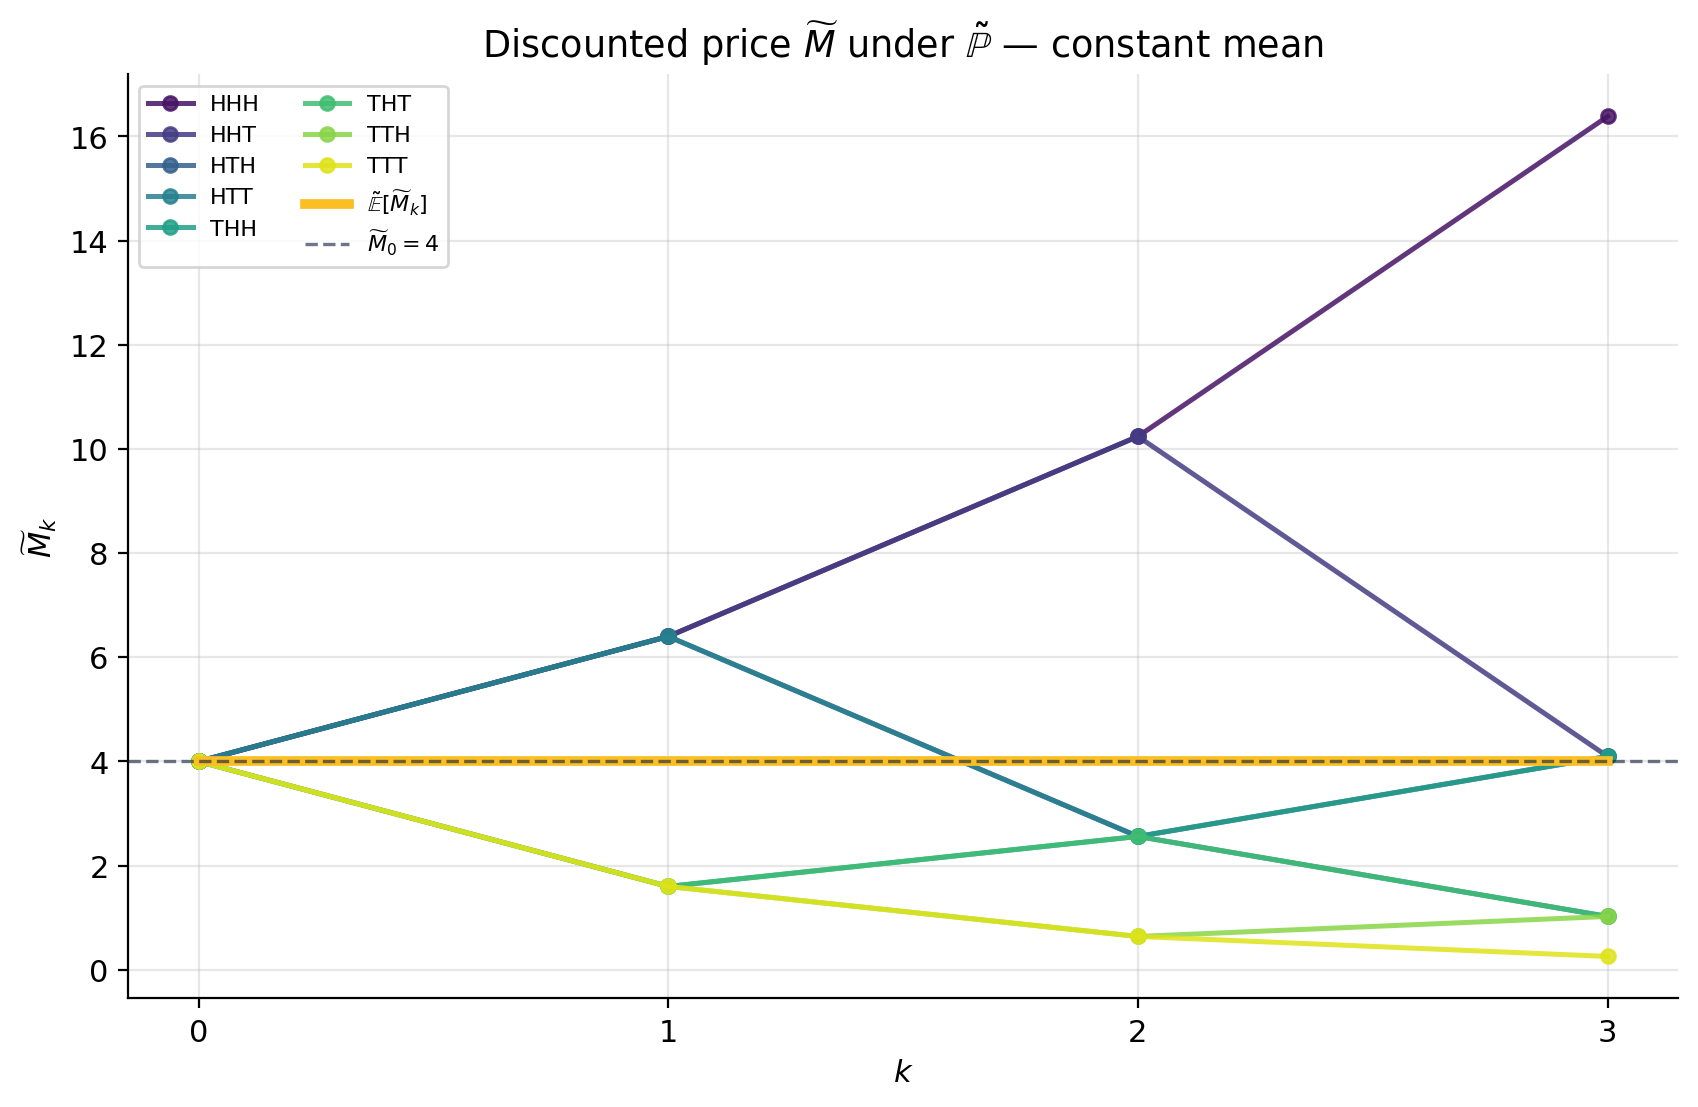
\includegraphics[keepaspectratio]{figures/ch03-martingale-paths.png}}
\caption{Eight paths of \(\widetilde M\) on Toy, \(n=3\), plotted vs
\(k\). Each path oscillates around the constant \(\widetilde M_0 = 4\).
The cross-sectional average at every \(k\) equals \(4\) --- that's the
martingale property, visible to the eye.}
\end{figure}

\begin{figure}
\centering
\pandocbounded{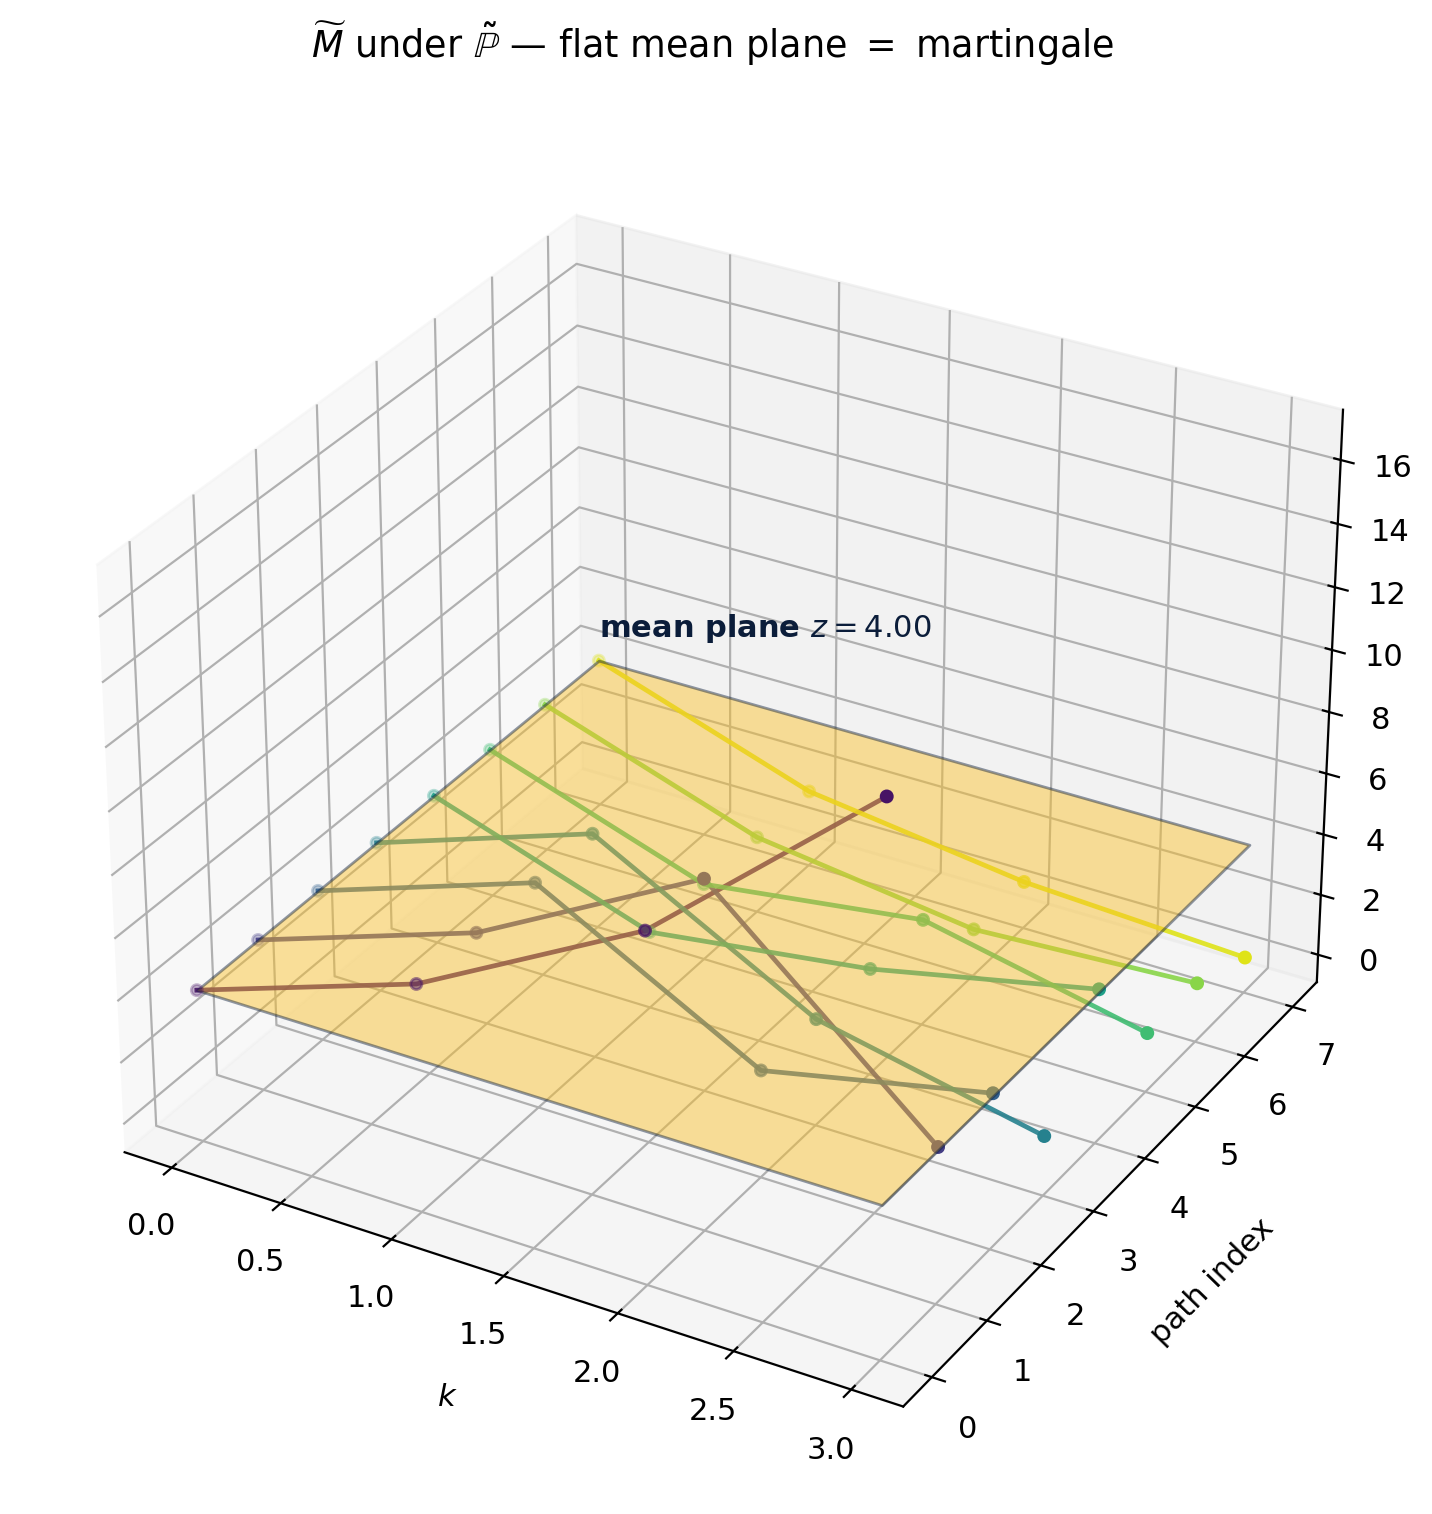
\includegraphics[keepaspectratio]{figures/ch03-Mtilde-3d.png}}
\caption{3-D surface over \((k, \text{path})\) of \(\widetilde M_k\)
under \(\tilde{\mathbb P}\). Paths are colourful and visit different
heights, but the time-\(k\) cross-sectional mean (the gold flat plane at
\(z=4\)) is constant in \(k\). Visually: ``fluctuation around a flat
plane'' \(=\) martingale.}
\end{figure}

\begin{figure}
\centering
\pandocbounded{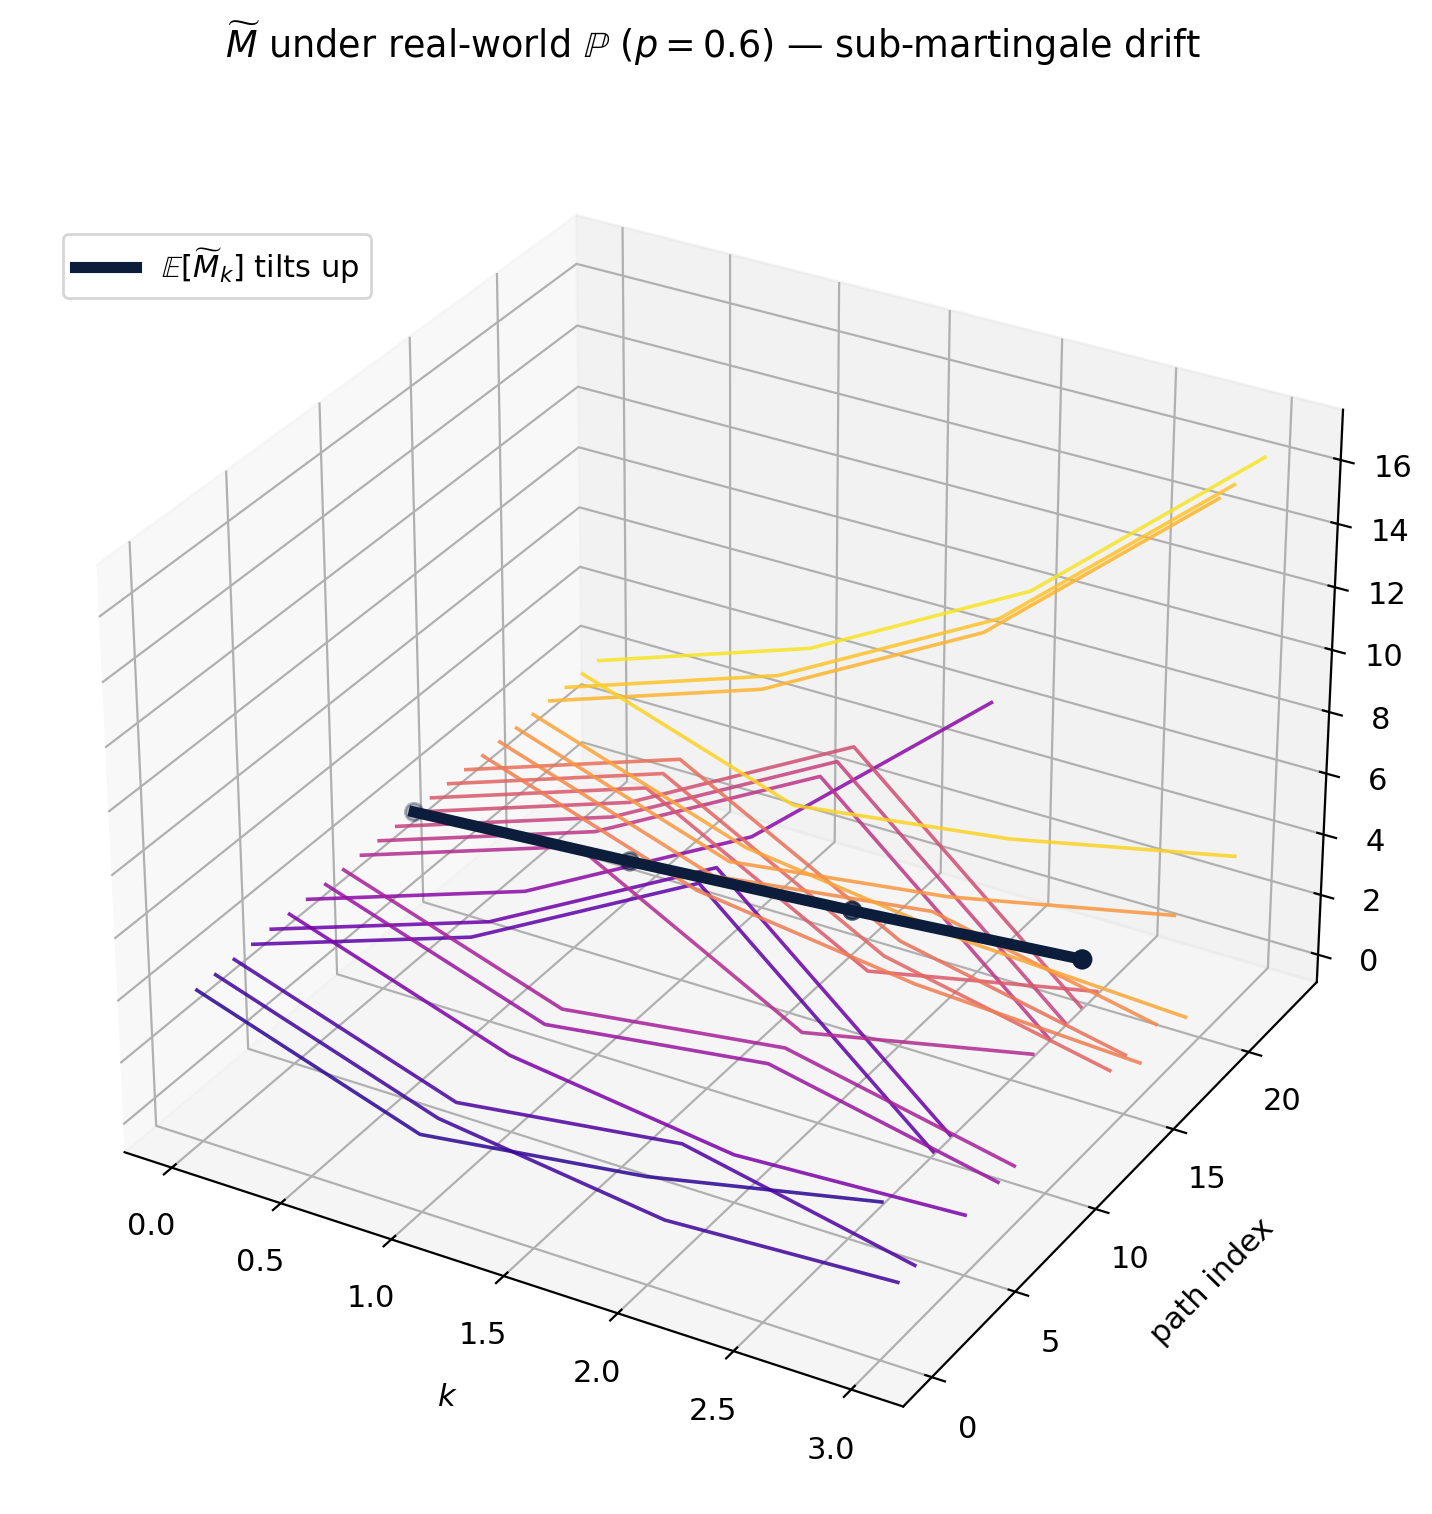
\includegraphics[keepaspectratio]{figures/ch03-Mtilde-P-3d.png}}
\caption{Same picture under real-world \(\mathbb P\) with \(p = 0.6\).
The 24 random paths drift up on average (sub-martingale); the dark
expected-path line tilts upward instead of staying flat. Risk premium
made visible.}
\end{figure}

\subsection{3.8.4 Table}\label{table-11}

\textbf{Table 3.8.} Process / measure / martingale class for the toy.

{\def\LTcaptype{none} % do not increment counter
\begin{table}[H]
\centering
\begin{tabular}{|l|l|l|r|}
\toprule
Process & Measure & Class & Drift factor \\
\midrule



\(S_k\) & \(\tilde{\mathbb P}\) & sub-mart. & \(1+r\) \\
\(S_k\) & \(\mathbb P\), \(p=0.6\) & sub-mart. & \(1.4\) \\
\(\widetilde M_k = S_k/(1+r)^k\) & \(\tilde{\mathbb P}\) &
\textbf{mart.} & \(1\) \\
\(\widetilde M_k\) & \(\mathbb P\), \(p=0.6\) & sub-mart. & \(1.12\) \\
\(V_k\) (European) & \(\tilde{\mathbb P}\) & sub-mart. &
\(\approx 1+r\) \\
\(\widetilde V_k\) (disc.) & \(\tilde{\mathbb P}\) & \textbf{mart.} &
\(1\) \\
\(X_k\) (wealth) & \(\tilde{\mathbb P}\) & sub-mart. & \(1+r\) \\
\(\widetilde X_k\) (disc.) & \(\tilde{\mathbb P}\) & \textbf{mart.} &
\(1\) \\
\bottomrule
\end{tabular}
\end{table}
}

\emph{Legend.} ``Drift factor'' = the one-step ratio
\(\mathbb E[Y_{k+1}\mid\mathcal F_k]/Y_k\). \emph{Numbers (Toy,
\(r=1/4\), \(u=2, d=1/2\)).} \(S\) under \(\tilde{\mathbb P}\):
\((0.5\cdot 2 + 0.5\cdot 0.5) = 1.25 = 1+r\). \(S\) under \(\mathbb P\),
\(p=0.6\): \(0.6\cdot 2 + 0.4\cdot 0.5 = 1.40\). \(\widetilde M\) under
\(\mathbb P\): \(1.4/1.25 = 1.12\).

\begin{center}\rule{0.5\linewidth}{0.5pt}\end{center}

\section{§3.9 Stopping times}\label{stopping-times}

\textbf{Punchline.} A \emph{stopping time} is a ``when to quit'' rule
that uses only past information. \(\tau\) is a stopping time if for
every \(k\), the event \(\{\tau \le k\}\) is in \(\mathcal F_k\) ---
i.e.~by time \(k\) you can tell whether you've already stopped.

\textbf{Intuition.} ``Sell the stock the first time it touches \$110.''
This rule is realisable --- you can check the condition as time
progresses. \emph{Not realisable}: ``sell the stock the last time it's
below \$95 between now and expiry'' --- this requires knowledge of the
future. The stopping-time condition is the formal way to forbid
clairvoyant exit rules. American option exercise must be a stopping
time.

\subsection{3.9.1 Definitions}\label{definitions-12}

A function \(\tau : \Omega_n \to \{0, 1, \ldots, n\} \cup \{\infty\}\)
is a \textbf{stopping time} with respect to \((\mathcal F_k)\) if for
every \(k \in \{0, 1, \ldots, n\}\),

\[\{\tau \le k\} \in \mathcal F_k.\]

Equivalent statements:

\begin{itemize}
\tightlist
\item
  \(\{\tau = k\} \in \mathcal F_k\) for every \(k\).
\item
  The indicator \(\mathbf 1_{\{\tau = k\}}\) is
  \(\mathcal F_k\)-measurable.
\item
  \(\tau\) is itself an ``adapted random variable'' in a precise sense.
\end{itemize}

A stopping time is \textbf{bounded} if \(\tau \le n\) almost surely (or
\(\tau \le N\) for some fixed \(N\)).

The \textbf{stopped process} \(X_{\tau \wedge k}\) takes the value
\(X_\tau\) if \(\tau \le k\), else \(X_k\). Conceptually: keep evolving
until \(\tau\), then freeze.

\subsection{3.9.2 Examples}\label{examples-19}

\textbf{Example 3.9.1 (\(\tau =\) first \(k\) with \(S_k \ge 8\), Toy,
\(n=3\)).} Walk through all 8 paths:

\begin{itemize}
\tightlist
\item
  \(HHH\): \(S_1=8 \ge 8\). \(\tau = 1\).
\item
  \(HHT\): \(S_1=8 \ge 8\). \(\tau = 1\).
\item
  \(HTH\): \(S_1=8 \ge 8\). \(\tau = 1\).
\item
  \(HTT\): \(S_1=8 \ge 8\). \(\tau = 1\).
\item
  \(THH\): \(S_1=2, S_2=4, S_3=8\). \(\tau = 3\).
\item
  \(THT\): \(S_1=2, S_2=4, S_3=2\). Never hits 8 within \(n=3\). By
  convention set \(\tau = 3\) (we cap at horizon) or \(\tau = \infty\)
  (we leave open).
\item
  \(TTH\): similar. \(\tau = 3\) or \(\infty\).
\item
  \(TTT\): \(\tau = 3\) or \(\infty\).
\end{itemize}

So all \(H\)-starting paths stop at \(k=1\); \(THH\) stops at \(k=3\);
the rest never hit. The minimum-of-horizon version
\(\tau \wedge n = \tau \wedge 3\) is \textbf{bounded} by 3.

\textbf{Example 3.9.2 (Verify \(\{\tau \le 1\} \in \mathcal F_1\)).}
\(\{\tau \le 1\} = \{HHH, HHT, HTH, HTT\} = A_H\). Yes, an
\(\mathcal F_1\)-event. ✓

\textbf{Example 3.9.3 (Verify \(\{\tau = 2\} \in \mathcal F_2\)).}
\(\{\tau = 2\} = \emptyset\) in this example (every path either stops at
1 or runs to \(\ge 3\)). The empty set is in every \(\mathcal F_k\). ✓

\textbf{Example 3.9.4 (Verify \(\{\tau = 3\} \in \mathcal F_3\)).}
\(\{\tau = 3\} = \{THH, THT, TTH, TTT\} = A_T\). This is even in
\(\mathcal F_1\), hence in \(\mathcal F_3\). ✓

\textbf{Example 3.9.5 (Non-example: ``last \(k\) with \(S_k = 4\)'').}
This rule needs to know the \emph{future} path to determine the
\emph{last} visit. On \(HTH\) (\(S = 4,8,4,8\)) the ``last visit to 4''
is \(k=2\), since \(S_3 = 8 \ne 4\). On \(HTT\) (\(S = 4,8,4,2\)) the
last visit to 4 is also \(k=2\), since \(S_3 = 2 \ne 4\). But to
\emph{announce} ``I'm stopping at \(k = 2\)'' on these paths, you must
already know \(S_3 \ne 4\) --- which lives in \(\mathcal F_3\), not
\(\mathcal F_2\). Formally, the event \(\{\tau = 2\}\) must lie in
\(\mathcal F_2\), but it doesn't: distinguishing \(HTH\) (where
\(\tau = 2\) is correct) from a hypothetical continuation that returns
to 4 later would require \(\mathcal F_3\). Bottom line: ``last visit''
is \emph{not} a stopping time --- the indicator of having stopped
depends on the future, which is forbidden.

\textbf{Example 3.9.6 (Realistic first-hit, \(\tau =\) first \(k\) with
\(S_k \ge 110\)).} \(S_0 = 100\). After one up-step, \(S_1 = 110\). So
all \(H\)-starting paths have \(\tau = 1\). Down-step path has
\(S_1 = 90\); from there it can hit 110 if subsequent moves are \(HH\)
(\$S\_3 = 99 \cdot 1.21 =\ldots{} \$ --- let me actually compute
properly. \(TH\): \(S_2 = 90 \cdot 1.10 = 99\). \(TT\): \(S_2 = 81\).
From \(TH\), an up gives \(108.9 < 110\); from \(TT\), up gives
\(89.1\). So no \(T\)-starting path hits 110 within \(n=3\).
\(\tau \wedge 3 = 1\) on \(\{\omega_1=H\}\) and \(\tau \wedge 3 = 3\)
elsewhere.

\textbf{Example 3.9.7 (\(\tau \wedge n\) is bounded).} For any stopping
time \(\tau\) and fixed horizon \(n\), \(\tau \wedge n\) takes values in
\(\{0,\ldots,n\}\). This is the form we'll use in OST. \emph{Always
bounded \(\implies\) OST applies.}

\textbf{Example 3.9.8 (Composition of stopping times).} If
\(\sigma, \tau\) are stopping times, so are \(\sigma \wedge \tau\),
\(\sigma \vee \tau\), \(\sigma + \tau\) (capped at \(n\)). Stopping
times form a lattice --- useful for combining ``exit rules''.

\textbf{Example 3.9.9 (Constant times).} \(\tau \equiv k\) is trivially
a stopping time: \(\{\tau \le j\}\) is \(\emptyset\) for \(j < k\) and
\(\Omega_n\) for \(j \ge k\), both in every \(\mathcal F_j\).

\textbf{Example 3.9.10 (Stopping time from a random variable).} If \(Y\)
is \(\mathcal F_n\)-measurable and you define
\(\tau = \mathbf 1_{\{Y = 1\}} \cdot 3 + \mathbf 1_{\{Y = 0\}} \cdot 1\),
\(\tau\) is \emph{not generally} a stopping time. The decision to stop
at 1 vs 3 depends on \(Y\), which lives in \(\mathcal F_n\) --- you
don't yet know it at time 1. So this is a ``rule'' but not a stopping
rule.

\begin{figure}
\centering
\pandocbounded{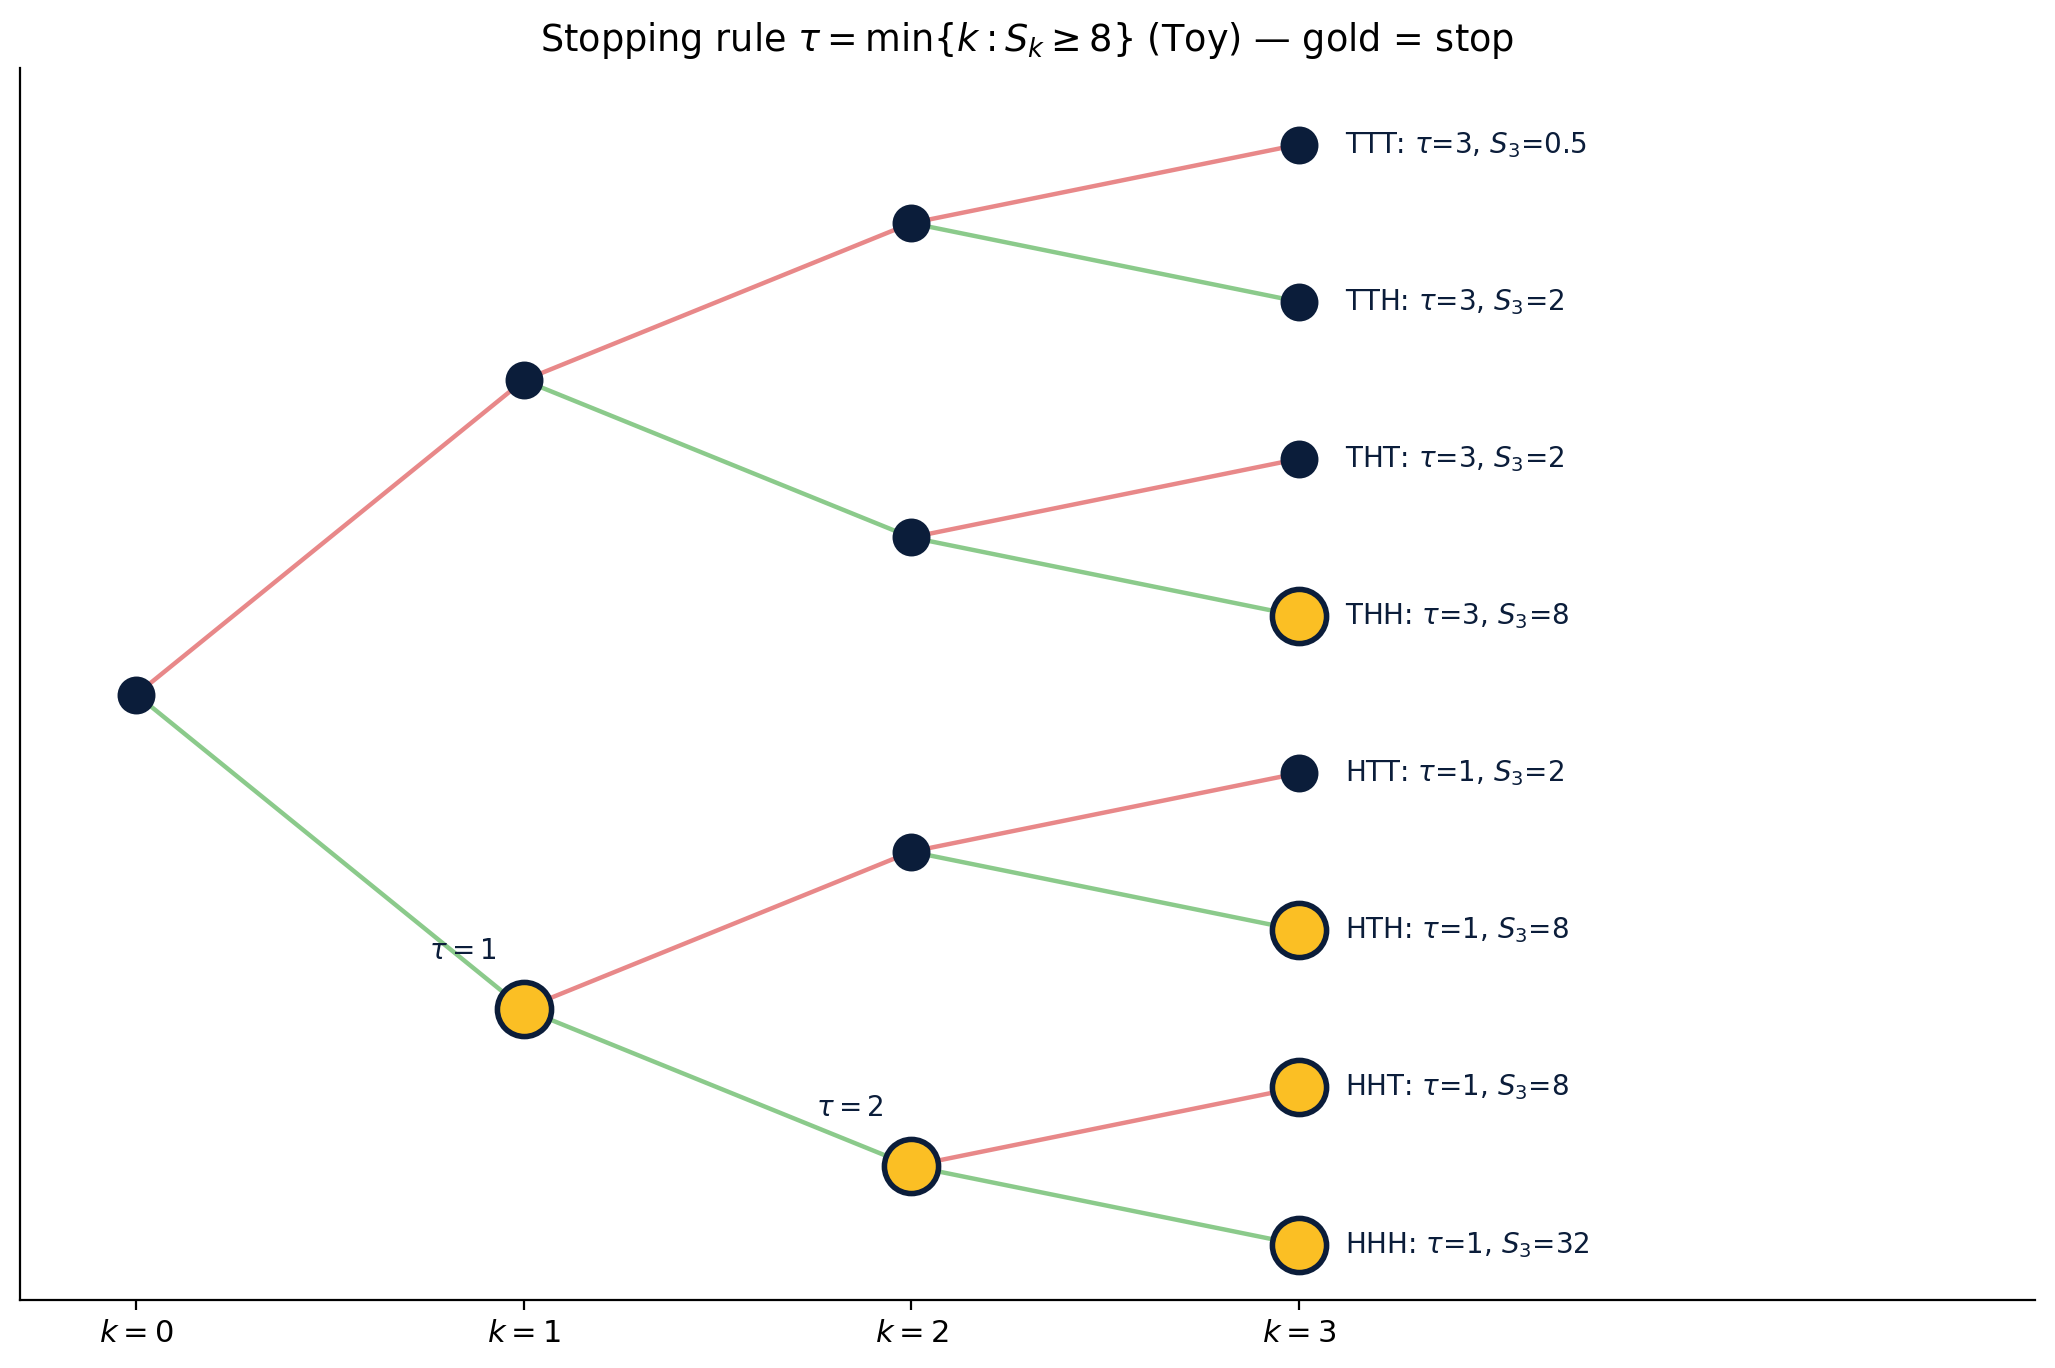
\includegraphics[keepaspectratio]{figures/ch03-stopping-tree.png}}
\caption{Tree on \(\Omega_3\) with stopping nodes circled in gold: the
stopping rule ``first \(k\) with \(S_k \ge 8\)'' on stops at the four
upper \(\mathcal F_1\)-nodes; for the lower paths it either stops at
\(k=3\) or never. Paths colour-coded by stop time.}
\end{figure}

\begin{figure}
\centering
\pandocbounded{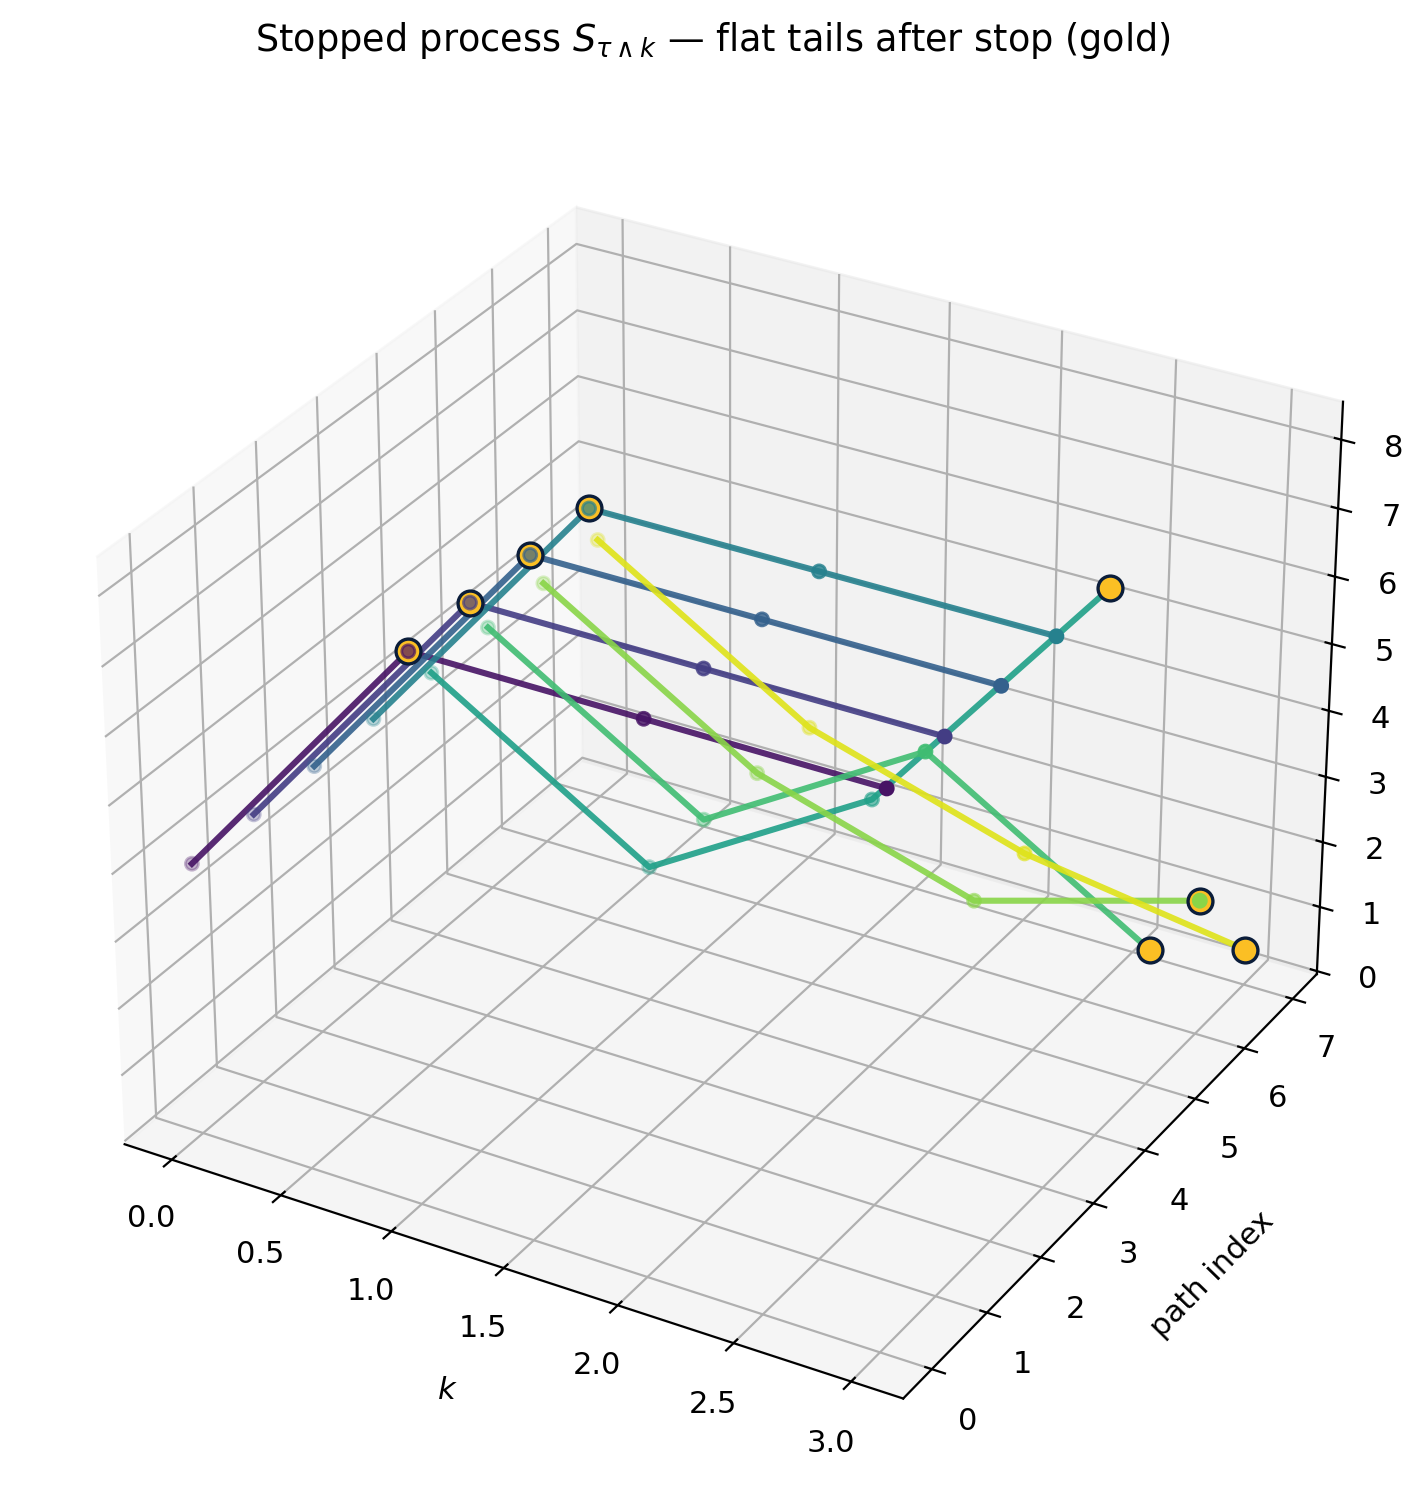
\includegraphics[keepaspectratio]{figures/ch03-stopped-3d.png}}
\caption{Stopped process \(S_{\tau \wedge k}\) for the same rule,
plotted in 3-D over \((k, \text{path}, S)\). Stopped paths
\emph{flatten} at the stop time --- visually obvious. The flat tail is
what makes optional stopping intuitive: no more contribution past
\(\tau\).}
\end{figure}

\subsection{3.9.3 Table}\label{table-12}

\textbf{Table 3.9.} Stopping rule
\(\tau = \min\{k : S_k \ge 8\} \wedge 3\) on \(\Omega_3\).

{\def\LTcaptype{none} % do not increment counter
\begin{table}[H]
\centering
\begin{tabular}{|l|r|r|r|r|r|}
\toprule
\(\omega\) & \(S_1\) & \(S_2\) & \(S_3\) & \(\tau\) & \(S_\tau\) \\
\midrule



\(HHH\) & 8 & 16 & 32 & 1 & 8 \\
\(HHT\) & 8 & 16 & 8 & 1 & 8 \\
\(HTH\) & 8 & 4 & 8 & 1 & 8 \\
\(HTT\) & 8 & 4 & 2 & 1 & 8 \\
\(THH\) & 2 & 4 & 8 & 3 & 8 \\
\(THT\) & 2 & 4 & 2 & 3 & 2 \\
\(TTH\) & 2 & 1 & 2 & 3 & 2 \\
\(TTT\) & 2 & 1 & 0.5 & 3 & 0.5 \\
\bottomrule
\end{tabular}
\end{table}
}

\begin{center}\rule{0.5\linewidth}{0.5pt}\end{center}

\section{§3.10 Optional stopping theorem
(stated)}\label{optional-stopping-theorem-stated}

\textbf{Punchline.} You can't beat a martingale with a bounded stopping
rule.

\[\mathbb E[M_\tau] = \mathbb E[M_0] \qquad \text{for any bounded stopping time } \tau.\]

\textbf{Intuition.} If \(M\) is fair (expected change zero), then
averaging over any \emph{legal} exit rule still gives back \(M_0\). Any
clever stopping rule that ``locks in gains'' is illusory because the
stopping rule cannot peek into the future. The boundedness is essential:
with an unbounded stop you can ``wait until you've doubled your money''
and pretend the random walk is favourable.

\subsection{3.10.1 Theorem statement (discrete time, finite
horizon)}\label{theorem-statement-discrete-time-finite-horizon}

Let \((M_k)_{k=0}^n\) be a martingale and \(\tau\) a stopping time with
\(\tau \le n\). Then \(\mathbb E[M_\tau] = \mathbb E[M_0] = M_0\) (when
\(M_0\) is constant). More generally, for any stopping time
\(\tau \le n\) and any \(k \le n\),

\[\mathbb E[M_\tau \mid \mathcal F_k] = M_{\tau \wedge k}.\]

The discrete-time, bounded-stopping version requires \emph{no
integrability conditions} beyond what we already have on a finite
probability space; the result is essentially a re-summation.

\subsection{3.10.2 Examples}\label{examples-20}

\textbf{Example 3.10.1 (Toy, \(\widetilde M_\tau\) check).} Stopping
rule \(\tau\) from §3.9 (first \(k\) with \(S_k \ge 8\), capped at
\(n=3\)). Compute \(\tilde{\mathbb E}[\widetilde M_\tau]\):

\begin{itemize}
\tightlist
\item
  On \(\{HHH, HHT, HTH, HTT\}\), \(\tau = 1\).
  \(\widetilde M_1(H) = 8/1.25 = 6.4\).
\item
  On \(\{THH\}\), \(\tau = 3\), \(S_3 = 8\),
  \(\widetilde M_3 = 8/(1.25)^3 = 8/1.953125 = 4.096\).
\item
  On \(\{THT, TTH\}\), \(\tau = 3\), \(S_3 = 2\),
  \(\widetilde M_3 = 2/1.953125 = 1.024\).
\item
  On \(\{TTT\}\), \(\tau = 3\), \(S_3 = 0.5\),
  \(\widetilde M_3 = 0.5/1.953125 = 0.256\).
\end{itemize}

\(\tilde{\mathbb P}\)-weights are uniform \(1/8\) over \(\Omega_3\).
Total:

\[
\begin{aligned}
\tilde{\mathbb E}[\widetilde M_\tau]
&= \tfrac{1}{8}(6.4 \cdot 4 + 4.096 + 1.024 + 1.024 + 0.256) \\
&= \tfrac{1}{8}(25.6 + 6.4) \;=\; \tfrac{32}{8} \;=\; 4 \;=\; \widetilde M_0.
\end{aligned}
\]

✓ OST verified.

\textbf{Example 3.10.2 (\(\tau \equiv 0\)).}
\(\tilde{\mathbb E}[\widetilde M_0] = 4 = \widetilde M_0\). ✓

\textbf{Example 3.10.3 (\(\tau \equiv 3\)).}
\(\tilde{\mathbb E}[\widetilde M_3] = \tilde{\mathbb E}[S_3/(1.25)^3]\).
We computed
\(\tilde{\mathbb E}[S_3] = (1.25)^3 \cdot 4 = 1.953125 \cdot 4 = 7.8125\).
So \(\tilde{\mathbb E}[\widetilde M_3] = 7.8125 / 1.953125 = 4\). ✓

\textbf{Example 3.10.4 (Different rule, same answer).} Rule ``first
\(k\) with \(S_k \le 2\)'': stops at \(k=1\) on the four \(T\)-starting
paths; stops at \(k=2\) on \(HTT\); stops at \(k=3\) on the rest (or
never). Compute \(\widetilde M_\tau\) leaf-by-leaf and sum; the answer
is again 4. \emph{This is the OST in action.}

\textbf{Example 3.10.5 (Put-call parity from OST).} Define \(P_k\) as
the put price, \(C_k\) as the call price. \(\widetilde P_k\) and
\(\widetilde C_k\) are both \(\tilde{\mathbb P}\)-martingales. So
\(\widetilde C_k - \widetilde P_k\) is a
\(\tilde{\mathbb P}\)-martingale. At expiry \(k=n\):
\(C_n - P_n = S_n - K\). Discount:
\(\widetilde C_n - \widetilde P_n = \widetilde S_n - K/(1+r)^n\). OST
applied to the martingale \(\widetilde C - \widetilde P\) at
\(\tau = n\) gives:
\[C_0 - P_0 = \tilde{\mathbb E}[\widetilde C_n - \widetilde P_n] = S_0 - K/(1+r)^n.\]
That's put-call parity, no calculus.

\textbf{Example 3.10.6 (Gambler's ruin sketch).} Suppose \(S\) is a
simple symmetric random walk on \(\mathbb Z\) starting at \(S_0 = a\),
with absorbing barriers at \(0\) and \(N\). \(M_k = S_k\) is a
martingale. Let \(\tau = \min\{k : S_k \in \{0, N\}\}\); OST (with care
--- \(\tau\) is unbounded but \(S_{\tau \wedge k}\) is bounded between
\(0\) and \(N\), so dominated convergence applies) gives
\(\mathbb E[S_\tau] = a\). But \(S_\tau \in \{0, N\}\), so if
\(q := \mathbb P(S_\tau = N)\), then \(qN = a\) ⇒ \(q = a/N\). The
classical formula.

\textbf{Example 3.10.7 (Counter-example with unbounded \(\tau\)).} Let
\(M_k\) be the simple symmetric random walk on \(\mathbb Z\),
\(M_0 = 0\), \(M_{k+1} - M_k \in \{+1, -1\}\) each with probability
\(1/2\). \(M\) is a martingale. Define
\(\tau = \min\{k \ge 1 : M_k = 1\}\) --- the first time the walk hits
level \(1\). Recurrence of the simple random walk gives
\(\tau < \infty\) a.s., so \(M_\tau = 1\) almost surely and
\(\mathbb E[M_\tau] = 1 \ne 0 = M_0\). OST fails because \(\tau\) is
\emph{unbounded} (no fixed cap) and the stopped process
\(M_{\tau \wedge k}\) is \emph{not} uniformly integrable --- it can
wander arbitrarily far negative before the eventual hit. The lesson: OST
\emph{requires} boundedness of \(\tau\), or a substitute integrability
condition.

\textbf{Example 3.10.8 (Verification for the rule ``stop at first \(k\)
where \(\widetilde M_k > 6\)'' on Toy, \(n=3\)).} On \(H\) paths,
\(\widetilde M_1 = 6.4 > 6\), stop. On \(T\) paths,
\(\widetilde M_1 = 1.6\), continue. At \(k=2\) on \(T\):
\(\widetilde M_2\) values: \(TH \to 2.56\), \(TT \to 0.64\). Neither
\(> 6\). At \(k=3\): \(\widetilde M_3\) values: \(THH = 4.096\), others
smaller. Never crosses 6 on \(T\) paths. So \(\tau = 1\) on \(H\) paths,
\(\tau = 3\) on \(T\) paths (cap).
\(\tilde{\mathbb E}[\widetilde M_\tau] = 0.5 \cdot 6.4 + 0.5 \cdot \tilde{\mathbb E}[\widetilde M_3 \mid T] = 0.5 \cdot 6.4 + 0.5 \cdot 1.6 = 4 = \widetilde M_0\).
✓ (Conditional
\(\tilde{\mathbb E}[\widetilde M_3 \mid T] = \widetilde M_1(T) = 1.6\)
by the martingale property.)

\begin{figure}
\centering
\pandocbounded{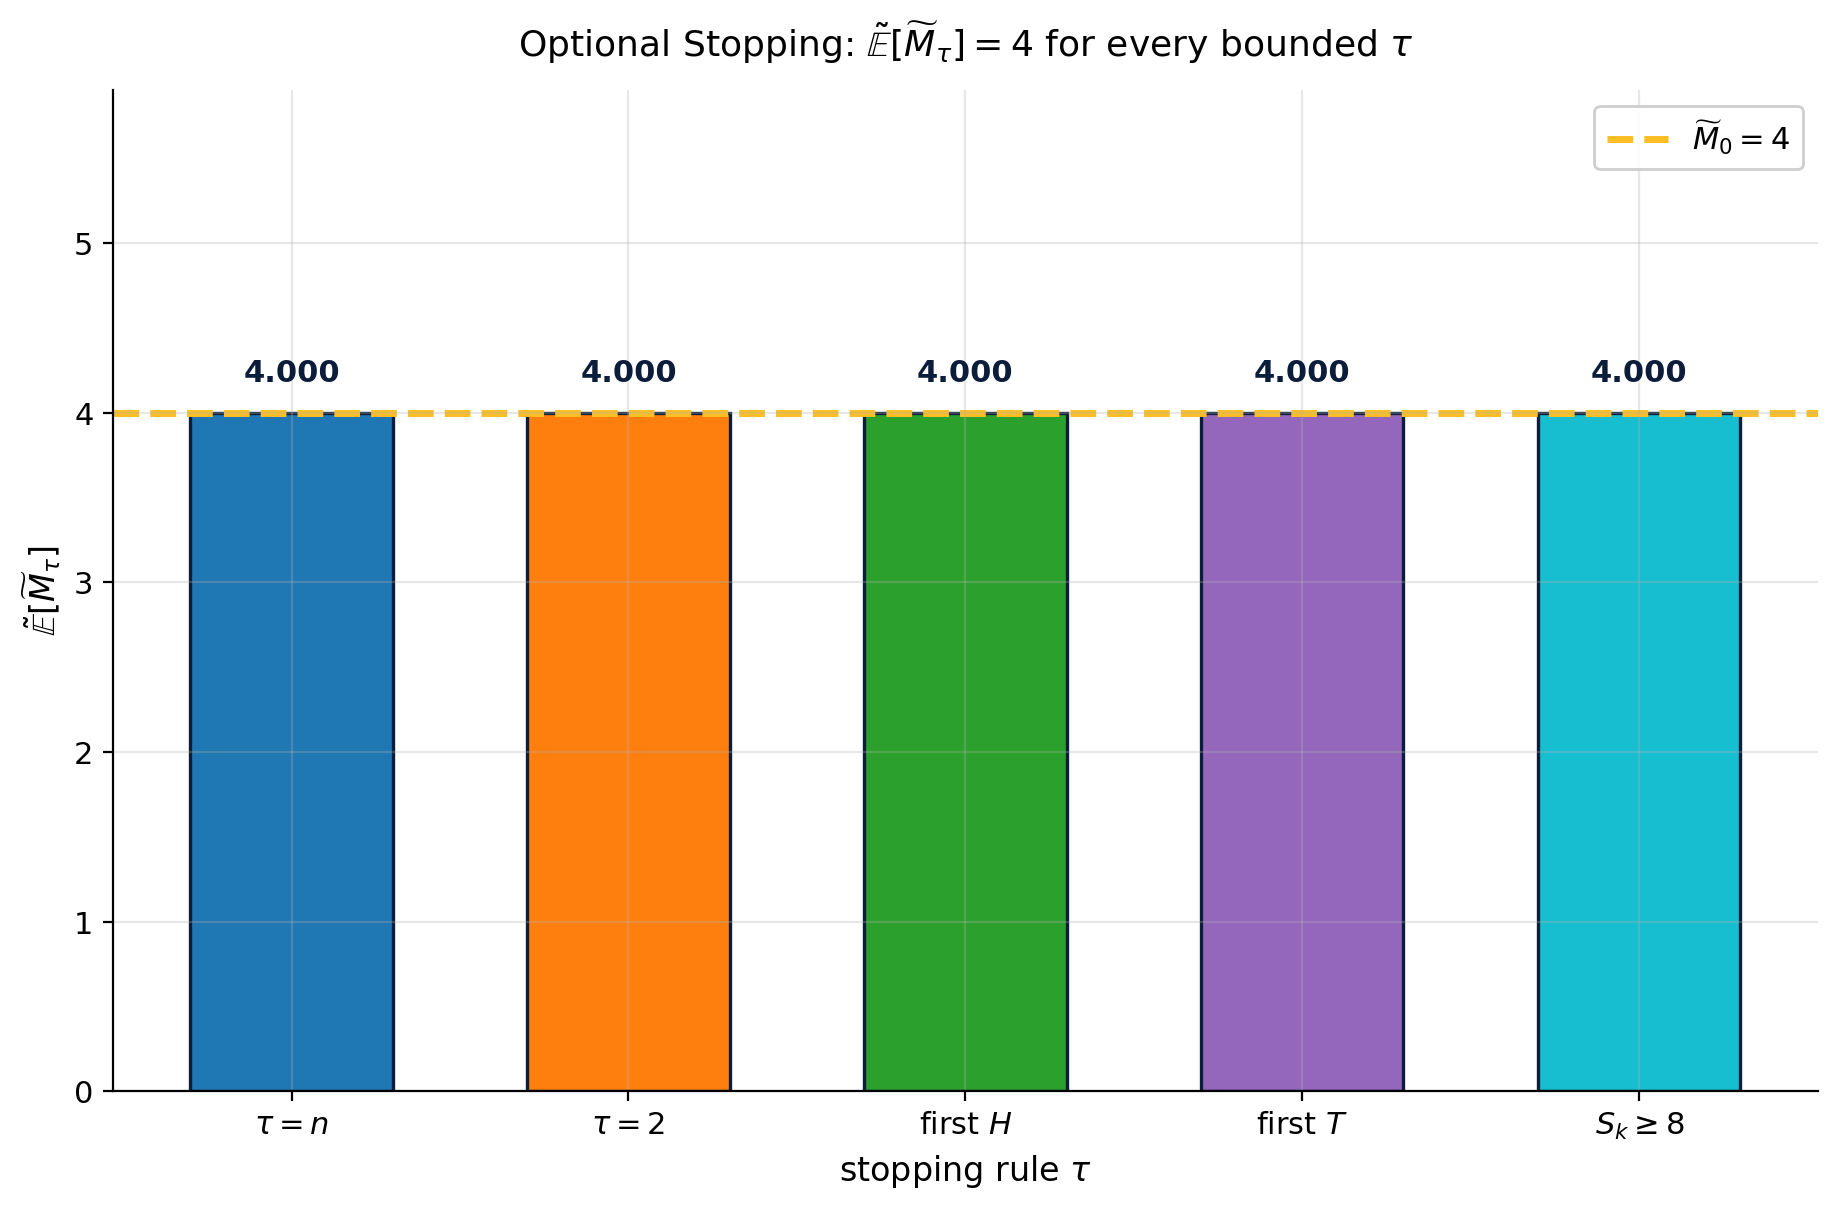
\includegraphics[keepaspectratio]{figures/ch03-ost-bars.png}}
\caption{Bar chart of \(\tilde{\mathbb E}[\widetilde M_\tau]\) for five
different bounded stopping rules on Toy. Every bar is at exactly 4 ---
the optional stopping theorem in one picture. The dashed line marks
\(\widetilde M_0 = 4\).}
\end{figure}

\subsection{3.10.3 Table}\label{table-13}

\textbf{Table 3.10.} OST verification on \(\Omega_3\) under
\(\tilde{\mathbb P}\).

{\def\LTcaptype{none} % do not increment counter
\begin{table}[H]
\centering
\begin{tabular}{|l|l|r|l|}
\toprule
Rule & Description & \(\tilde{\mathbb E}[\widetilde M_\tau]\) & Check \\
\midrule



\(\tau \equiv 0\) & Don't stop & \(4\) & ✓ \\
\(\tau \equiv 3\) & Wait to expiry & \(4\) & ✓ \\
First \(k, S_k \ge 8\) & Take profit & \(4\) & ✓ \\
First \(k, S_k \le 2\) & Cut loss & \(4\) & ✓ \\
First \(k, \widetilde M_k > 6\) & Discounted threshold & \(4\) & ✓ \\
\bottomrule
\end{tabular}
\end{table}
}

\begin{center}\rule{0.5\linewidth}{0.5pt}\end{center}

\section{§3.11 Change of measure: real-world vs
risk-neutral}\label{change-of-measure-real-world-vs-risk-neutral}

\textbf{Punchline.} \(\mathbb P\) and \(\tilde{\mathbb P}\) live on the
\textbf{same paths}. They differ only in the \textbf{weights} assigned
to those paths. Two measures that agree on which events have probability
zero are called \emph{equivalent}.

\textbf{Intuition.} Imagine the eight leaves of \(\Omega_3\) as eight
little buckets. Pour 100 ml of ``real-world ink'' into them with weights
\(\binom{3}{j} p^j (1-p)^{3-j}\), \(p=0.6\). Pour 100 ml of
``risk-neutral ink'' with weights
\(\binom{3}{j} \tilde p^j (1-\tilde p)^{3-j}\), \(\tilde p = 0.5\). Same
buckets, two different distributions of ink. The \emph{ratio} of ink
levels in each bucket is the Radon-Nikodym density
\(Z(\omega) = \tilde{\mathbb P}(\{\omega\}) / \mathbb P(\{\omega\})\).

\subsection{3.11.1 Definitions}\label{definitions-13}

Two probability measures \(\mathbb P, \tilde{\mathbb P}\) on the finite
space \(\Omega_n\) are \textbf{equivalent}, denoted
\(\mathbb P \sim \tilde{\mathbb P}\), if they assign positive mass to
exactly the same singletons:

\[\mathbb P(\{\omega\}) > 0 \iff \tilde{\mathbb P}(\{\omega\}) > 0 \quad \text{for all } \omega.\]

On \(\Omega_n = \{H,T\}^n\) with \(p, \tilde p \in (0,1)\) both strictly
between 0 and 1, this is automatic.

The \textbf{Radon-Nikodym density} of \(\tilde{\mathbb P}\) with respect
to \(\mathbb P\) is the random variable

\[Z(\omega) \;=\; \frac{\tilde{\mathbb P}(\{\omega\})}{\mathbb P(\{\omega\})} \;=\; \left(\frac{\tilde p}{p}\right)^{H_n(\omega)} \left(\frac{1-\tilde p}{1-p}\right)^{n - H_n(\omega)}.\]

The fundamental relation:

\[\tilde{\mathbb P}(A) \;=\; \mathbb E_{\mathbb P}[Z\cdot \mathbf 1_A] \quad\text{for every } A.\]

Equivalently, for any random variable \(X\),

\[\tilde{\mathbb E}[X] \;=\; \mathbb E[Z \cdot X].\]

\subsection{3.11.2 Examples}\label{examples-21}

\textbf{Example 3.11.1 (Compute \(Z\) on \(\Omega_2\)).} \(n=2\),
\(p=0.6\), \(\tilde p=0.5\). - \(HH\): \(\mathbb P = 0.36\),
\(\tilde{\mathbb P} = 0.25\), \(Z = 0.25/0.36 = 0.6944\). - \(HT\):
\(\mathbb P = 0.24\), \(\tilde{\mathbb P} = 0.25\), \(Z = 1.0417\). -
\(TH\): \(\mathbb P = 0.24\), \(\tilde{\mathbb P} = 0.25\),
\(Z = 1.0417\). - \(TT\): \(\mathbb P = 0.16\),
\(\tilde{\mathbb P} = 0.25\), \(Z = 1.5625\).

\textbf{Example 3.11.2 (Verify \(\mathbb E[Z] = 1\)).}
\(\mathbb E[Z] = 0.36 \cdot 0.6944 + 0.24 \cdot 1.0417 + 0.24 \cdot 1.0417 + 0.16 \cdot 1.5625 = 0.25 + 0.25 + 0.25 + 0.25 = 1.00\).
✓ (\(\mathbb E[Z] = 1\) always --- direct from
\(\tilde{\mathbb P}(\Omega) = 1\).)

\textbf{Example 3.11.3 (Closed form for \(Z\)).}
\(Z(\omega) = (\tilde p/p)^{H_n} ((1-\tilde p)/(1-p))^{n-H_n}\). On Toy
with \(p=0.6\) and \(\tilde p = 0.5\):
\(\tilde p/p = 5/6 \approx 0.8333\),
\((1-\tilde p)/(1-p) = 0.5/0.4 = 1.25\). So
\(Z = (5/6)^{H_n} \cdot (5/4)^{n - H_n}\).

\textbf{Example 3.11.4 (Realistic, \(n=2\)).} \(p=0.6\),
\(\tilde p = 0.6\) --- they coincide if and only if \(\tilde p = p\).
Boring. Let's use \(p = 0.55\). Then \(\tilde p/p = 0.6/0.55 = 1.0909\),
\((1-\tilde p)/(1-p) = 0.4/0.45 = 0.8889\).
\(Z(HH) = 1.0909^2 = 1.1900\),
\(Z(HT) = Z(TH) = 1.0909 \cdot 0.8889 = 0.9697\),
\(Z(TT) = 0.8889^2 = 0.7901\).

\textbf{Example 3.11.5 (\(\tilde p\) on Toy \(= 0.5\) regardless of
\(p\)).} The risk-neutral \(\tilde p\) depends \emph{only} on
\(u, d, r\), not on the real-world \(p\). That's the deep content of the
Chapter 1 derivation. \(\mathbb P\) varies with the real world;
\(\tilde{\mathbb P}\) is pinned by no-arbitrage. The RN density \(Z\)
measures the gap.

\textbf{Example 3.11.6 (Recover \(\tilde{\mathbb E}[S_2]\) via
\(\mathbb E[Z\,S_2]\) on Toy, \(n=2\)).} \(S_2\) values:
\(\{16, 4, 4, 1\}\) at \(\{HH, HT, TH, TT\}\). \(Z\) values from Example
3.11.1: \(\{0.6944, 1.0417, 1.0417, 1.5625\}\). \(\mathbb P\)-weights:
\(\{0.36, 0.24, 0.24, 0.16\}\).

\(\mathbb E[Z S_2] = 0.36(0.6944)(16) + 0.24(1.0417)(4) + 0.24(1.0417)(4) + 0.16(1.5625)(1) = 4.0 + 1.0 + 1.0 + 0.25 = 6.25\).

Cross-check:
\(\tilde{\mathbb E}[S_2] = (\tilde p u + (1-\tilde p) d)^2 \cdot S_0 = 1.25^2 \cdot 4 = 6.25\).
✓

\textbf{Example 3.11.7 (Recover \(\tilde{\mathbb E}\) on Toy, \(n=3\)).}
\(\tilde{\mathbb E}[S_3] = (1.25)^3 \cdot 4 = 7.8125\). Same number via
\(\mathbb E[Z S_3]\) --- the eight leaves contribute
\(\mathbb P(\omega) Z(\omega) S_3(\omega)\), summing to \(7.8125\).

\textbf{Example 3.11.8 (Independence of paths preserved).} Under
\(\mathbb P\), the flips are independent. Under \(\tilde{\mathbb P}\),
they are still independent (the joint factorises with \(\tilde p\)
replacing \(p\)). \(Z\) tilts the marginal but not the independence
structure.

\textbf{Example 3.11.9 (Bayes-rule version).} For any event \(A\):
\(\tilde{\mathbb P}(A) = \mathbb E_{\mathbb P}[Z\,\mathbf 1_A]\) ---
interpret \(Z\) as a ``Bayes factor'' reweighting events from the real
world to the risk-neutral world.

\begin{figure}
\centering
\pandocbounded{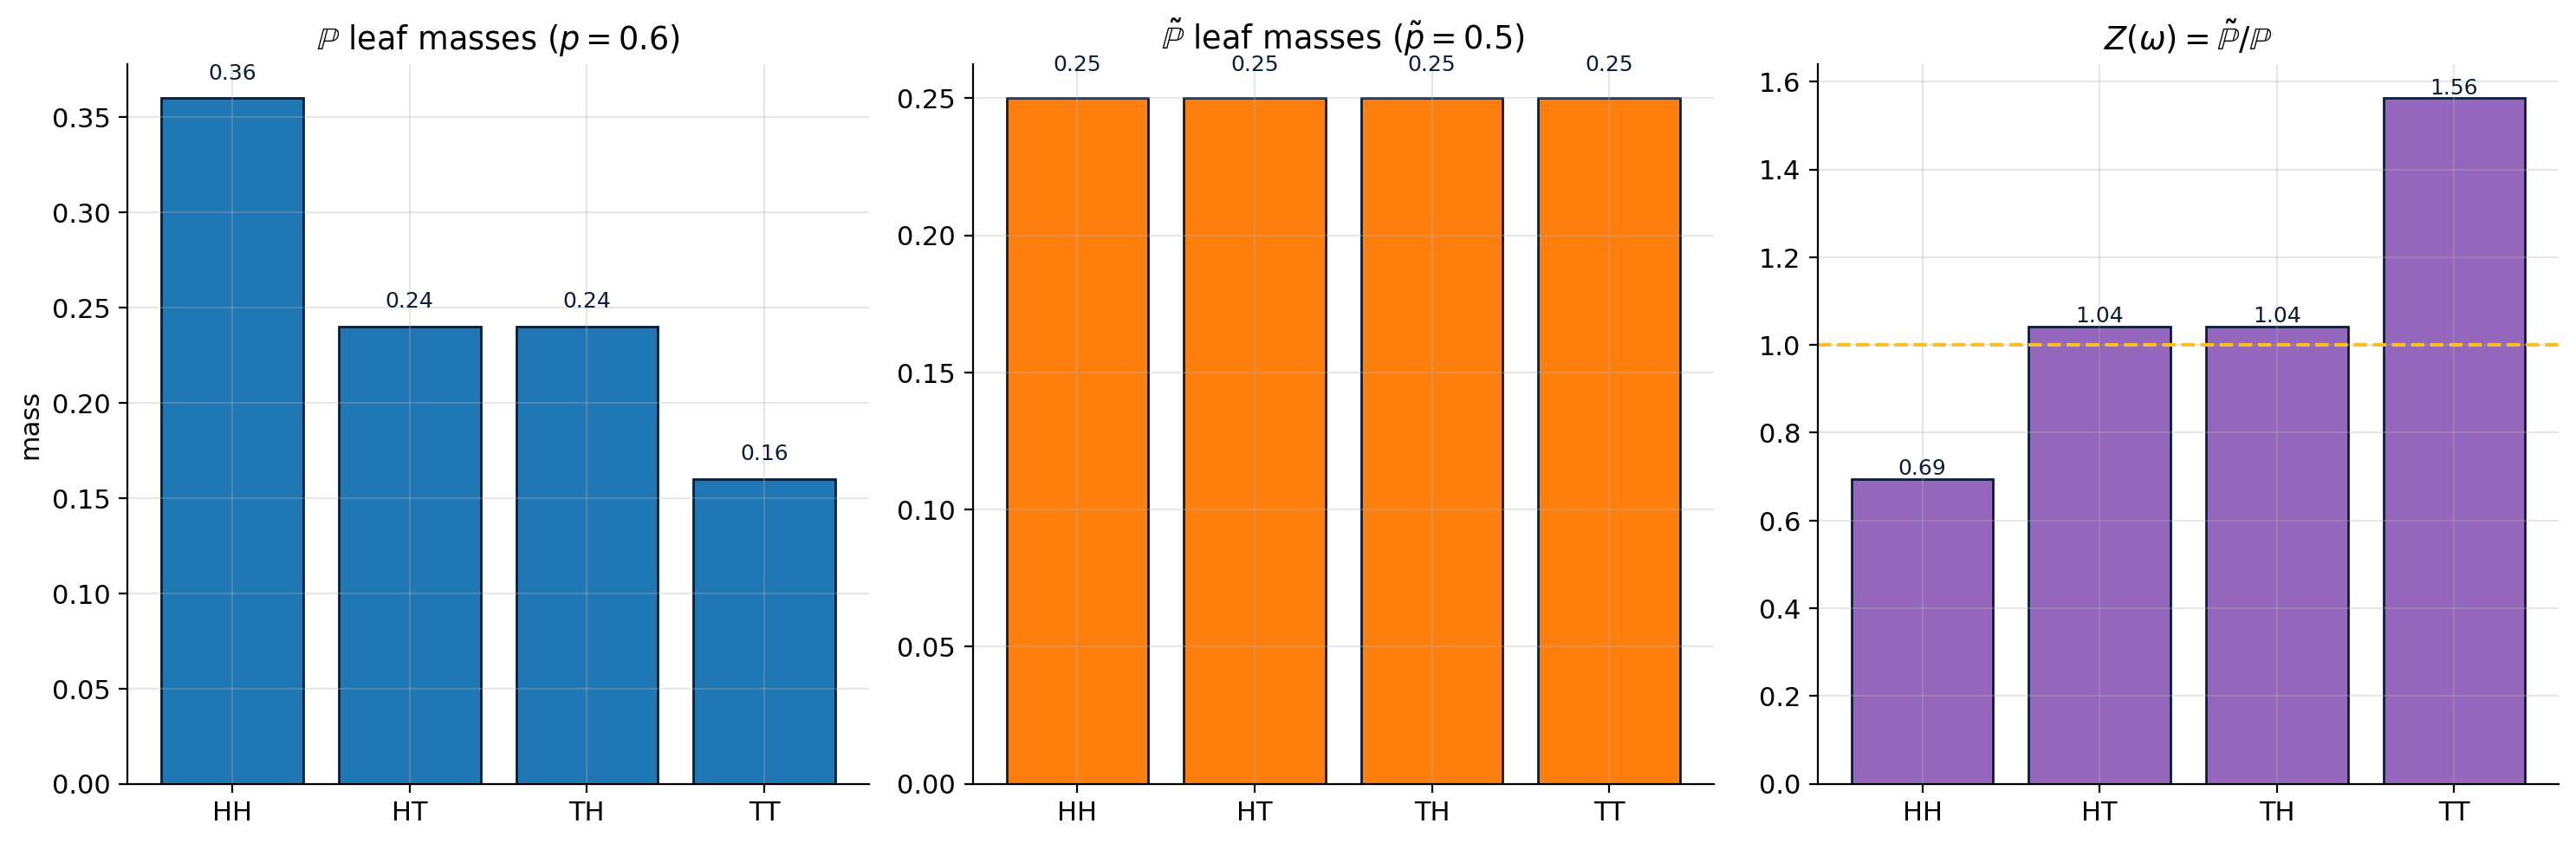
\includegraphics[keepaspectratio]{figures/ch03-change-of-measure-bars.png}}
\caption{Three bar charts side by side: leaf masses on \(\Omega_2\)
under real-world \(\mathbb P\) (\(p=0.6\)), under risk-neutral
\(\tilde{\mathbb P}\) (\(\tilde p=0.5\)), and the leaf-wise ratio
\(Z = \tilde{\mathbb P}/\mathbb P\). The first two redistribute mass
across the same four leaves; the third reads off the redistribution per
leaf.}
\end{figure}

\begin{figure}
\centering
\pandocbounded{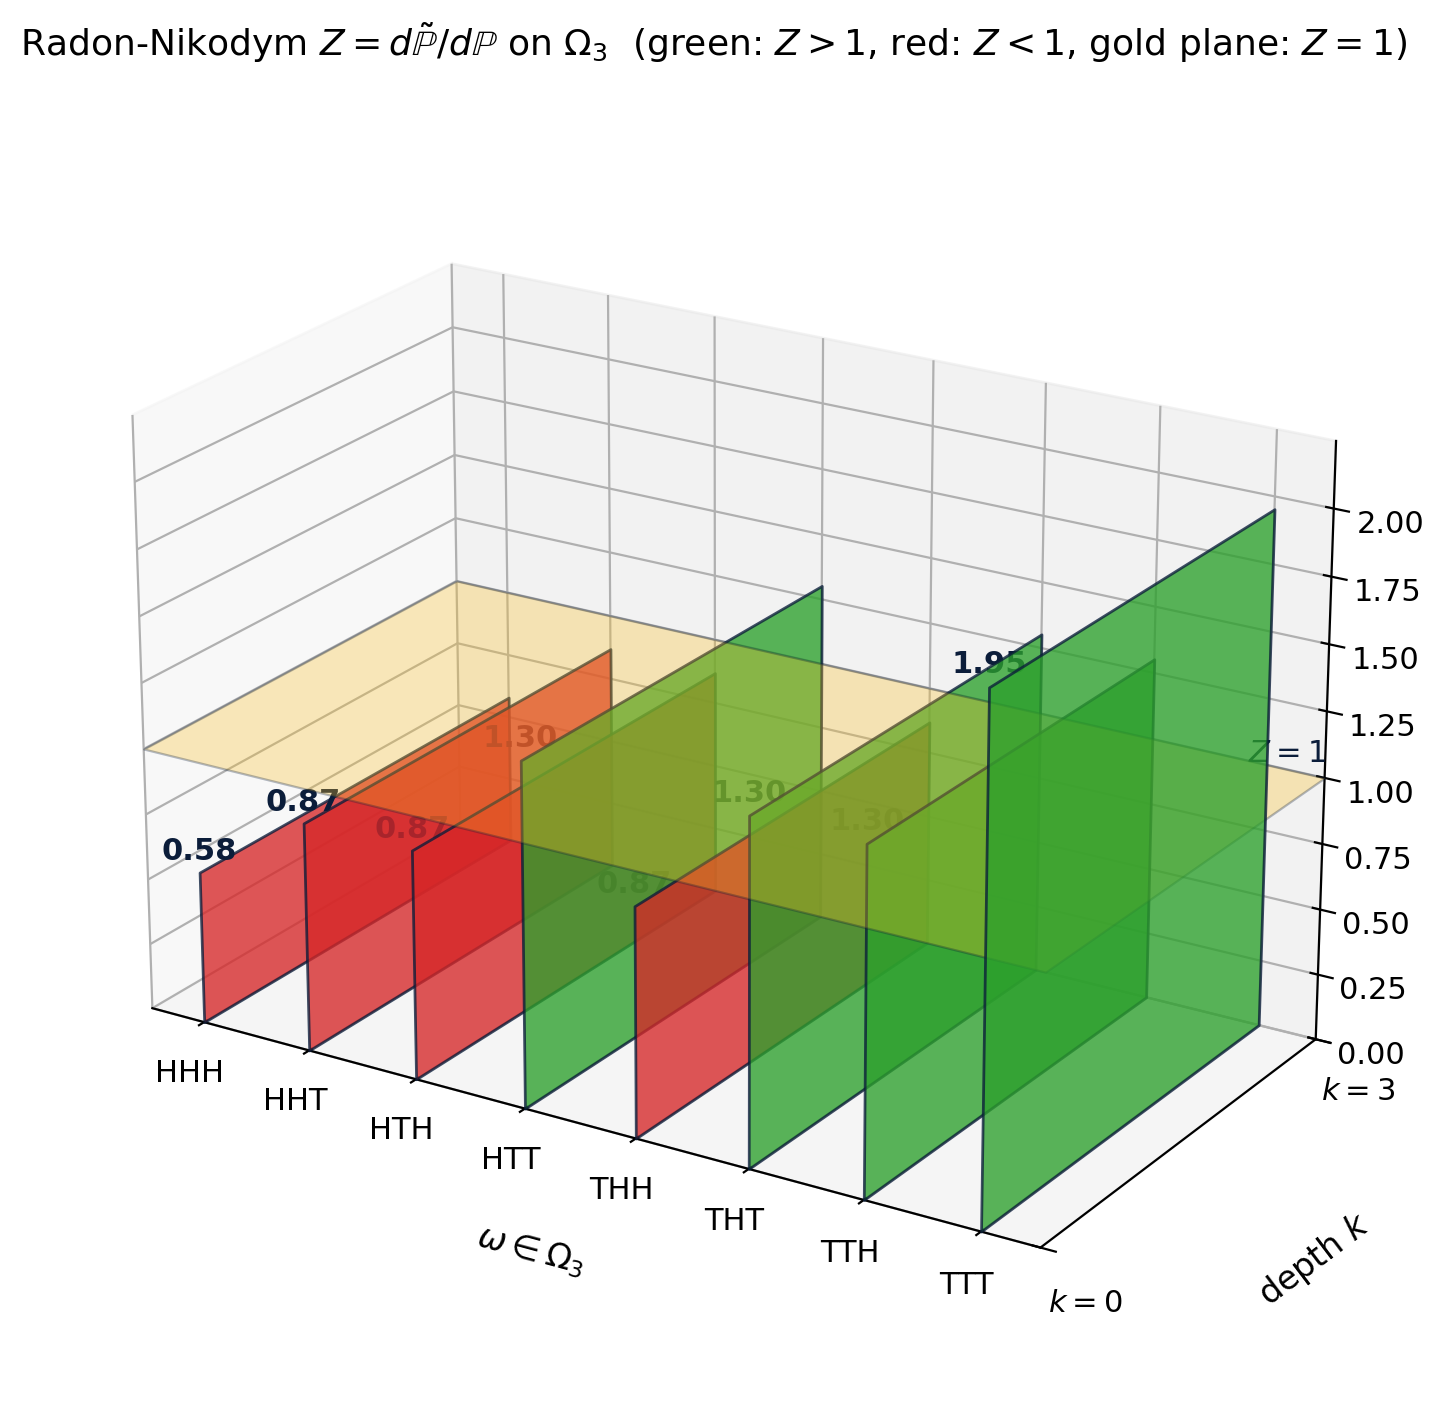
\includegraphics[keepaspectratio]{figures/ch03-Z-3d-bar.png}}
\caption{3-D bars: \(Z(\omega)\) over the eight sample points of
\(\Omega_3\). The lone full-heads leaf is \emph{down-weighted} under
\(\tilde{\mathbb P}\) (\(Z < 1\)); the full-tails leaf is
\emph{up-weighted} (\(Z > 1\)). Intuitively, the real world thinks heads
are more likely than the risk-neutral measure does, so the risk-neutral
measure compensates by putting \emph{more} weight on tail-heavy paths.}
\end{figure}

\subsection{3.11.3 Table}\label{table-14}

\textbf{Table 3.11.} Radon-Nikodym density on \(\Omega_2\), \(p=0.6\),
\(\tilde p = 0.5\).

{\def\LTcaptype{none} % do not increment counter
\begin{table}[H]
\centering
\begin{tabular}{|l|r|r|r|r|}
\toprule
\(\omega\) & \(\mathbb P(\{\omega\})\) & \(\tilde{\mathbb P}(\{\omega\})\) & \(Z(\omega)\) & \(Z \cdot \mathbb P\) \\
\midrule



\(HH\) & \(0.36\) & \(0.25\) & \(0.6944\) & \(0.25\) \\
\(HT\) & \(0.24\) & \(0.25\) & \(1.0417\) & \(0.25\) \\
\(TH\) & \(0.24\) & \(0.25\) & \(1.0417\) & \(0.25\) \\
\(TT\) & \(0.16\) & \(0.25\) & \(1.5625\) & \(0.25\) \\
Sum & \(1.00\) & \(1.00\) & (n/a) & \(1.00\) \\
\bottomrule
\end{tabular}
\end{table}
}

Notice the last column:
\(Z(\omega) \mathbb P(\{\omega\}) = \tilde{\mathbb P}(\{\omega\})\).
Multiplication by \(Z\) converts \(\mathbb P\)-leaf weights into
\(\tilde{\mathbb P}\)-leaf weights.

\begin{center}\rule{0.5\linewidth}{0.5pt}\end{center}

\section{§3.12 The Radon-Nikodym derivative as leaf-level
reweighting}\label{the-radon-nikodym-derivative-as-leaf-level-reweighting}

\textbf{Punchline.} \(Z = d\tilde{\mathbb P}/d\mathbb P\) is a
\emph{per-path} multiplier. The conditional version
\(Z_k := \mathbb E[Z \mid \mathcal F_k]\) --- called the
\textbf{martingale density} --- is itself a \(\mathbb P\)-martingale,
and it lets us ``translate'' expectations one \(\mathcal F_k\)-block at
a time.

\textbf{Intuition.} \(Z\) is just a function
\(\Omega_n \to \mathbb R_+\) telling you how to reweight each leaf. As
soon as you go to a \(\mathcal F_k\)-level (a partition coarser than
singletons), the leaf-by-leaf \(Z\) collapses into a \emph{block-level}
\(Z_k\) that lets you translate inside each block. The collapse is by
conditional expectation under \(\mathbb P\).

\subsection{3.12.1 Definitions and facts}\label{definitions-and-facts-2}

\textbf{Radon-Nikodym density}:
\(Z(\omega) = \tilde{\mathbb P}(\{\omega\})/\mathbb P(\{\omega\})\) on a
finite sample space.

\textbf{Martingale density} at time \(k\):
\(Z_k(\omega) := \mathbb E[Z \mid \mathcal F_k](\omega)\), the
\(\mathbb P\)-conditional expectation of \(Z\) given \(\mathcal F_k\).

\textbf{Key facts} (each provable in 2 lines on the finite space):

\begin{enumerate}
\def\labelenumi{\arabic{enumi}.}
\tightlist
\item
  \(Z_0 = \mathbb E[Z] = 1\), \(Z_n = Z\).
\item
  \((Z_k)\) is a \(\mathbb P\)-martingale:
  \(\mathbb E[Z_{k+1} \mid \mathcal F_k] = Z_k\).
\item
  For any \(\mathcal F_n\)-measurable \(X\):
  \(\tilde{\mathbb E}[X] = \mathbb E[Z\cdot X] = \mathbb E[Z_n\cdot X]\).
\item
  For \(\mathcal F_k\)-measurable \(X\):
  \(\tilde{\mathbb E}[X] = \mathbb E[Z_k \cdot X]\).
\item
  \textbf{Bayes rule for conditional expectation}:
  \(\tilde{\mathbb E}[X \mid \mathcal F_k] = \mathbb E[Z X \mid \mathcal F_k] / Z_k\),
  valid when \(Z_k > 0\) (always, in our finite setting with
  \(p, \tilde p \in (0,1)\)).
\end{enumerate}

\subsection{3.12.2 Examples}\label{examples-22}

\textbf{Example 3.12.1 (\(Z_1\) on Toy, \(p=0.6, \tilde p = 0.5\),
\(n=2\)).}

\begin{itemize}
\tightlist
\item
  \(Z_1(H) = \mathbb E[Z \mid \mathcal F_1 = A_H]\): average \(Z\) over
  the two leaves \(\{HH, HT\}\) weighted by their conditional
  \(\mathbb P\) masses. Conditional on \(A_H\), \(\omega_2 = H\) has
  prob \(p=0.6\), \(\omega_2 = T\) has prob \(0.4\). So
  \(Z_1(H) = 0.6 \cdot Z(HH) + 0.4 \cdot Z(HT) = 0.6 \cdot 0.6944 + 0.4 \cdot 1.0417 = 0.4167 + 0.4167 = 0.8333\).
  (Or via formula:
  \(Z_1(H) = (\tilde p/p)^{H_1}\cdot ((1-\tilde p)/(1-p))^{1-H_1}\cdot \mathbb E[(\tilde p/p)^{H_2-H_1}((1-\tilde p)/(1-p))^{1-(H_2-H_1)}] = (\tilde p/p)\cdot 1 = 5/6 \approx 0.8333\).)
\item
  \(Z_1(T) = (1-\tilde p)/(1-p) = 0.5/0.4 = 1.25\).
\end{itemize}

\textbf{Example 3.12.2 (\(Z_2\) on Toy, \(n=2\)).} \(Z_2 = Z\) --- at
the terminal time the conditional density equals the actual density.

\begin{itemize}
\tightlist
\item
  \(Z_2(HH) = 0.6944\), \(Z_2(HT) = Z_2(TH) = 1.0417\),
  \(Z_2(TT) = 1.5625\).
\end{itemize}

\textbf{Example 3.12.3 (Verify \(Z_1\) is a \(\mathbb P\)-martingale).}
\(\mathbb E[Z_1] = p \cdot Z_1(H) + (1-p) \cdot Z_1(T) = 0.6 \cdot 0.8333 + 0.4 \cdot 1.25 = 0.5 + 0.5 = 1.0 = Z_0\).
✓ Block check:
\(\mathbb E[Z_2 \mid \mathcal F_1 = A_H] = 0.6 Z(HH) + 0.4 Z(HT) = 0.8333 = Z_1(H)\).
✓

\textbf{Example 3.12.4 (\(\tilde{\mathbb E}[S_2]\) via \(Z_2\)).}
\(\tilde{\mathbb E}[S_2] = \mathbb E[Z_2 S_2] = 0.36 \cdot 0.6944 \cdot 16 + 0.24 \cdot 1.0417 \cdot 4 + 0.24 \cdot 1.0417 \cdot 4 + 0.16 \cdot 1.5625 \cdot 1 = 4 + 1 + 1 + 0.25 = 6.25\).
✓

\textbf{Example 3.12.5 (\(\tilde{\mathbb E}[S_1]\) via \(Z_1\)).}
\(\tilde{\mathbb E}[S_1] = \mathbb E[Z_1 S_1] = 0.6 \cdot 0.8333 \cdot 8 + 0.4 \cdot 1.25 \cdot 2 = 4 + 1 = 5\).
Cross-check:
\(\tilde{\mathbb E}[S_1] = (\tilde p u + (1-\tilde p) d) S_0 = 1.25 \cdot 4 = 5\).
✓

\textbf{Example 3.12.6 (Bayes-style price).} Price a one-step call with
strike \(K = 4\) under risk-neutral measure: payoff at \(S_1\) is
\((S_1 - 4)^+\). Under \(\tilde{\mathbb P}\):
\(\tilde{\mathbb E}[(S_1-4)^+] = 0.5(8-4) + 0.5(0) = 2\). Discounted:
\(2/1.25 = 1.6\). Via \(Z\):
\(\mathbb E[Z_1 (S_1-4)^+] = 0.6 \cdot 0.8333 \cdot 4 + 0.4 \cdot 1.25 \cdot 0 = 2.00\).
Same.

\textbf{Example 3.12.7 (Realistic call repricing, \(K = 100\),
\(n = 2\)).} Direct risk-neutral pricing: \(\tilde p = 0.6\), payoffs
\((S_2 - 100)^+ \in \{21, 0, 0, 0\}\) at \(\{HH, HT, TH, TT\}\) (since
\(S_2 \in \{121, 99, 99, 81\}\)); expectation
\(0.6^2 \cdot 21 = 0.36 \cdot 21 = 7.56\); discounted price
\(7.56/(1.02)^2 = 7.56/1.0404 \approx 7.27\). Recompute via \(Z\): pick
real-world \(p = 0.55\), so \(Z(HH) = (0.6/0.55)^2 = 1.1900\) from
Example 3.11.4. \(\mathbb P\)-weights:
\(\{0.3025, 0.2475, 0.2475, 0.2025\}\) for \(\{HH, HT, TH, TT\}\).
\(\mathbb E[Z \cdot (S_2-100)^+] = 0.3025 \cdot 1.19 \cdot 21 + 0 + 0 + 0 = 7.56\).
Discounted: \(7.56/1.0404 \approx 7.27\). Same answer. ✓

\textbf{Example 3.12.8 (Per-path multiplicative structure).} \(Z\) has
multiplicative structure across flips:
\(Z(\omega) = \prod_{i=1}^n L_i(\omega)\) where
\(L_i(\omega) = (\tilde p/p)\) if \(\omega_i = H\),
\(L_i(\omega) = (1-\tilde p)/(1-p)\) if \(\omega_i = T\). Then
\(Z_k(\omega) = \prod_{i=1}^k L_i(\omega)\), since the future
\(L_{k+1},\ldots,L_n\) have \(\mathbb P\)-expectation \(1\). This makes
\(Z_k\) a function of the first \(k\) flips alone ---
\(\mathcal F_k\)-measurable, as required.

\textbf{Example 3.12.9 (\(Z_k\) closed form).} From the multiplicative
structure:
\(Z_k(\omega) = (\tilde p/p)^{H_k(\omega)} \cdot ((1-\tilde p)/(1-p))^{k - H_k(\omega)}\).
This is the formula we plotted as a 3-D mesh.

\textbf{Example 3.12.10 (One-step martingale check).}
\(\mathbb E[Z_{k+1} \mid \mathcal F_k] = Z_k \cdot \mathbb E[L_{k+1}] = Z_k \cdot (p \cdot \tilde p/p + (1-p) \cdot (1-\tilde p)/(1-p)) = Z_k \cdot (\tilde p + 1 - \tilde p) = Z_k\).
✓ One line.

\begin{figure}
\centering
\pandocbounded{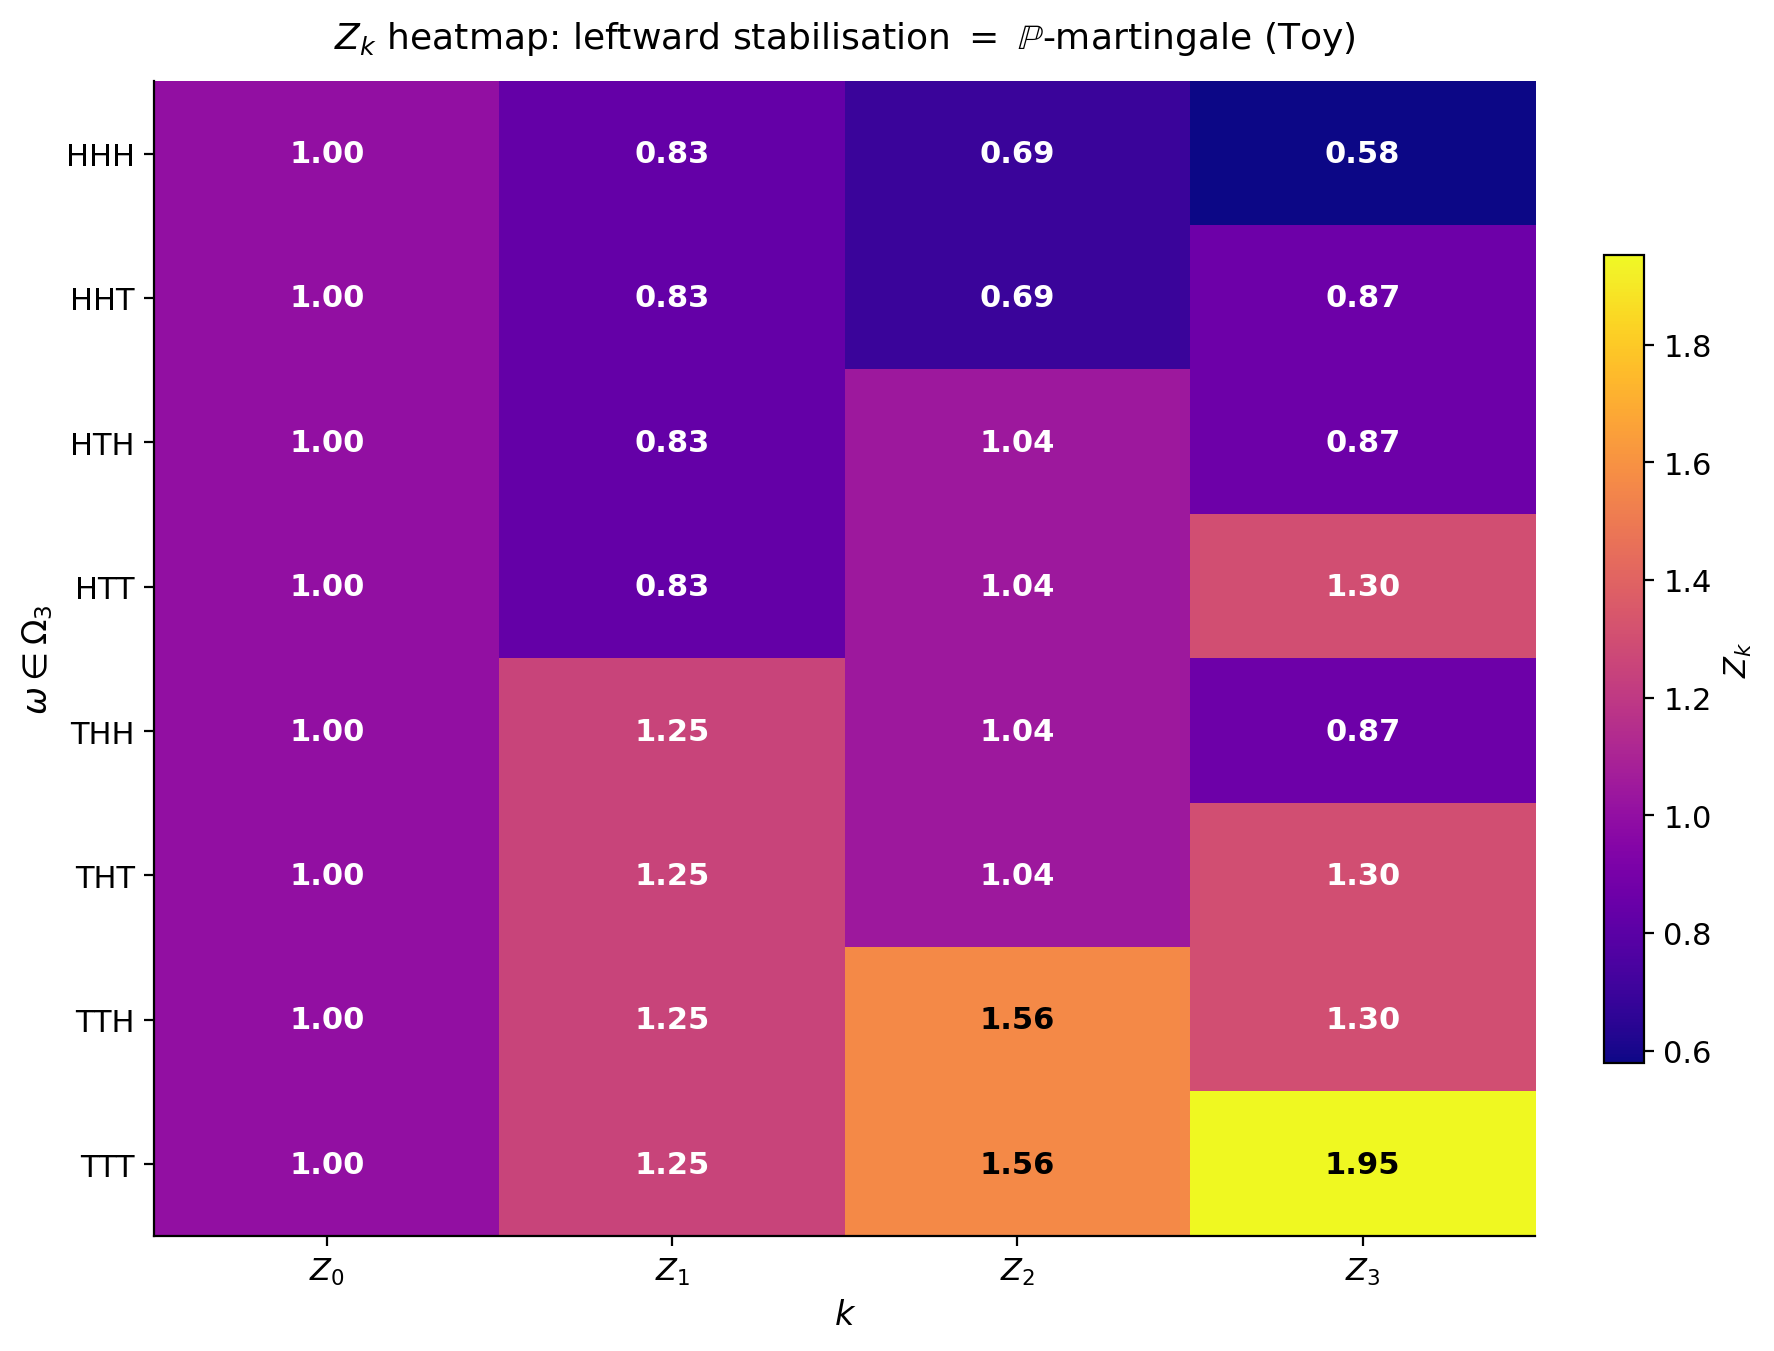
\includegraphics[keepaspectratio]{figures/ch03-Zk-heatmap.png}}
\caption{Heatmap with rows \(\omega \in \Omega_3\) and columns
\(Z_0, Z_1, Z_2, Z_3\) (Toy, \(p=0.6, \tilde p=0.5\)). The leftward
columns \emph{stabilise}: \(Z_0 = 1\) everywhere, \(Z_1\) takes one of
two values, \(Z_2\) four values, \(Z_3\) eight. \emph{Martingale =
leftward stabilisation}.}
\end{figure}

\begin{figure}
\centering
\pandocbounded{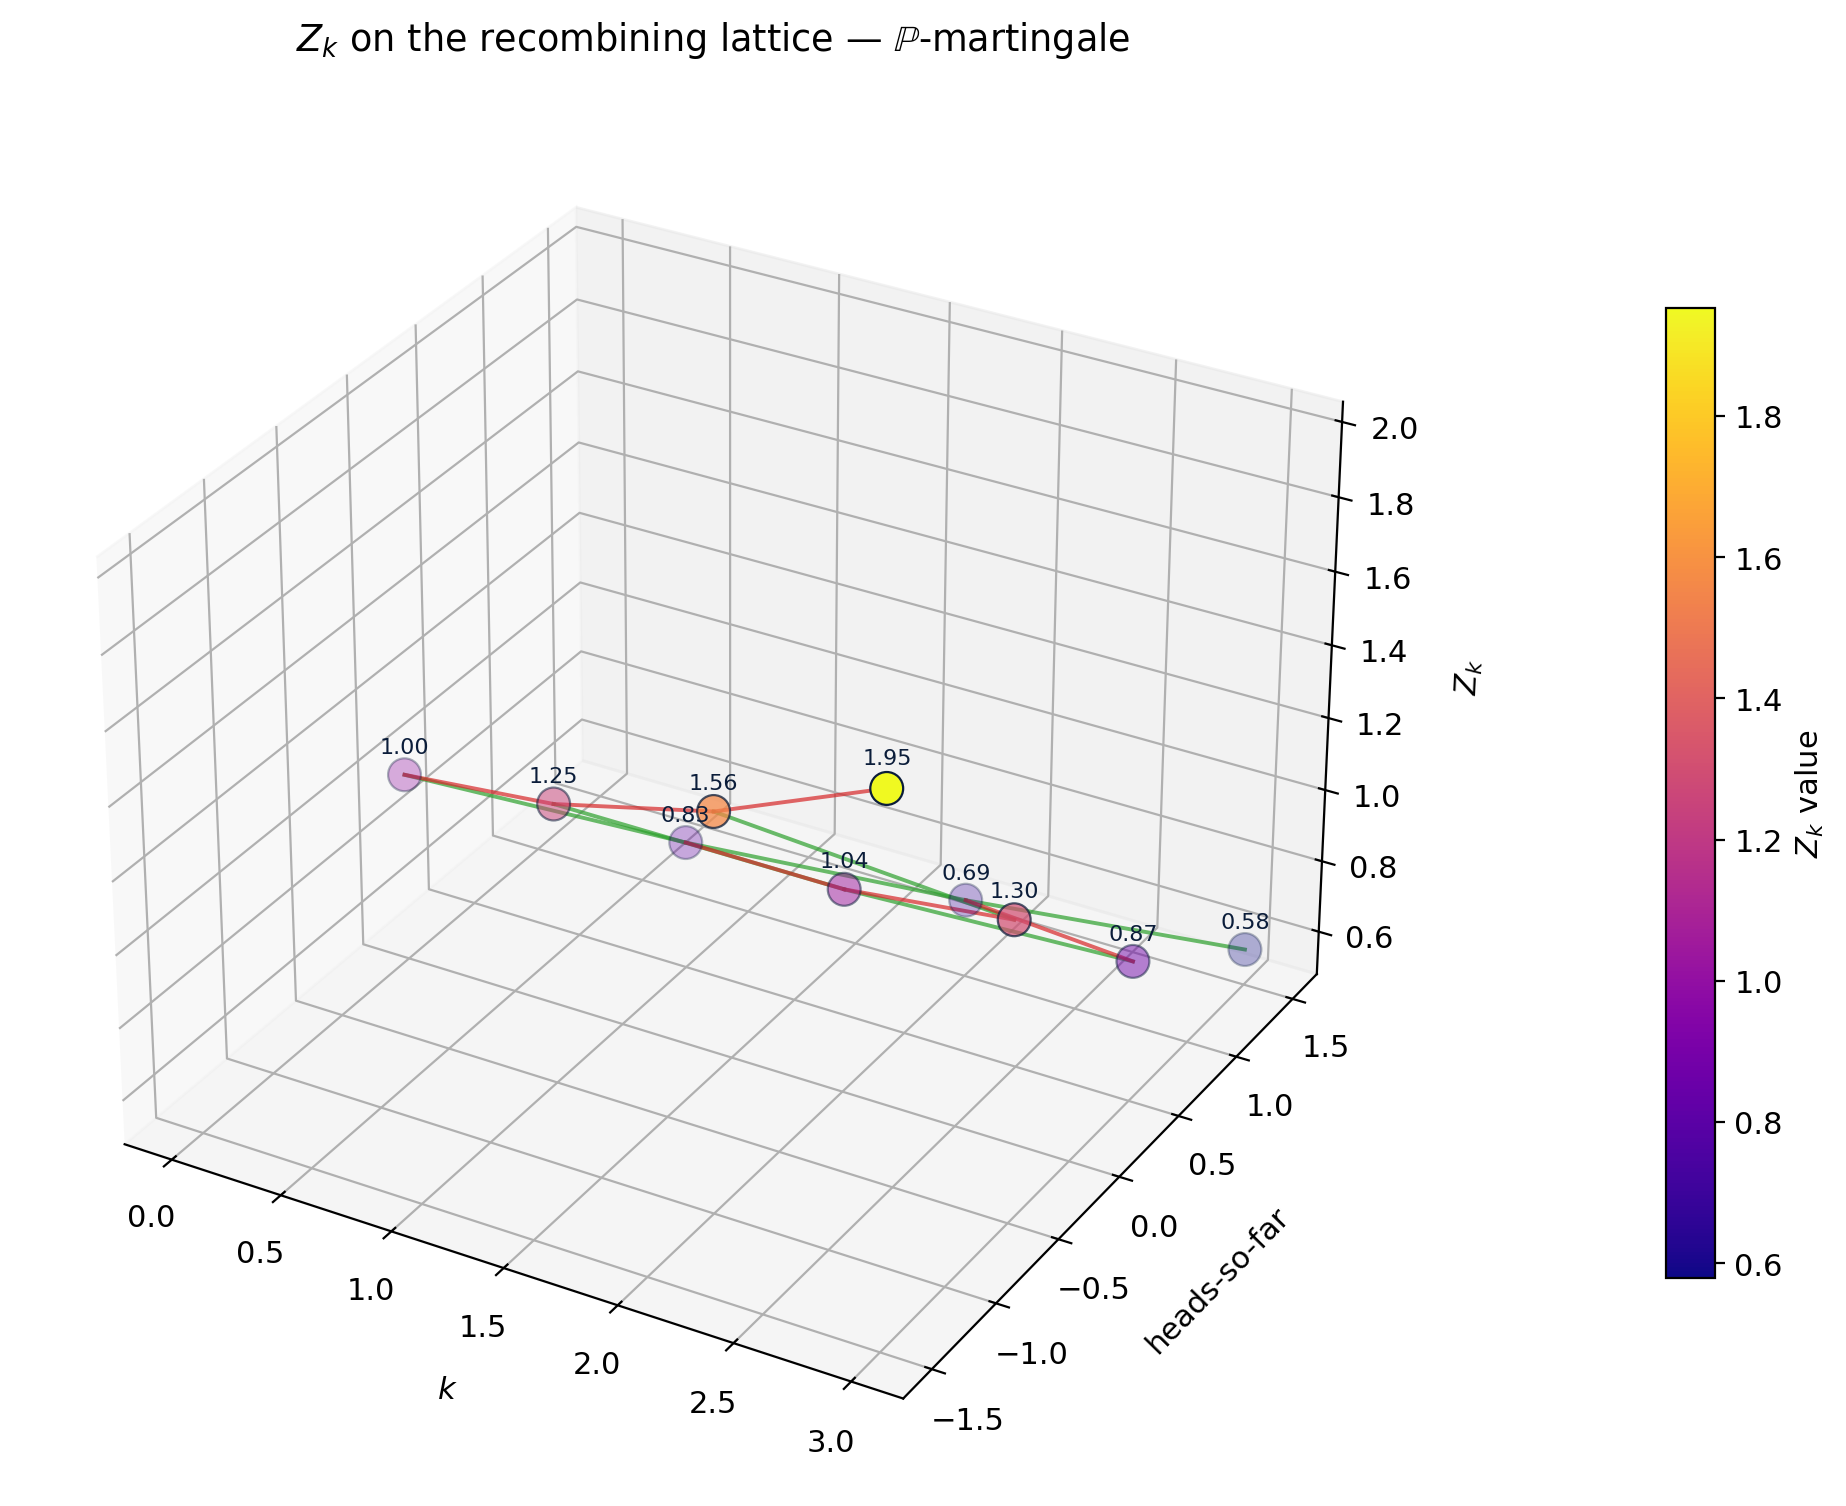
\includegraphics[keepaspectratio]{figures/ch03-Zk-mesh.png}}
\caption{3-D wire mesh of \(Z_k(\omega)\) over the recombining lattice
\((k, \text{number of heads so far})\). Nodes are colour-coded by
\(Z_k\) value; light edges show parent-child connections. The mesh
visualises a \(\mathbb P\)-martingale: each parent equals the
\(p\)-weighted average of its two children.}
\end{figure}

\subsection{3.12.3 Table}\label{table-15}

\textbf{Table 3.12.} Martingale density at every node of the
\(\Omega_2\) tree (\(p=0.6, \tilde p=0.5\)).

{\def\LTcaptype{none} % do not increment counter
\begin{table}[H]
\centering
\begin{tabular}{|l|r|r|r|r|}
\toprule
Node & \(\mathbb P\)-mass & \(\tilde{\mathbb P}\)-mass & \(Z_k\) & \(p\)-avg check \\
\midrule



Root, \(k=0\) & \(1.00\) & \(1.00\) & \(1.0000\) & \(1.000\) ✓ \\
\(H\), \(k=1\) & \(0.60\) & \(0.50\) & \(0.8333\) & \(0.8333\) ✓ \\
\(T\), \(k=1\) & \(0.40\) & \(0.50\) & \(1.2500\) & \(1.250\) ✓ \\
\(HH\), \(k=2\) & \(0.36\) & \(0.25\) & \(0.6944\) & leaf \\
\(HT\), \(k=2\) & \(0.24\) & \(0.25\) & \(1.0417\) & leaf \\
\(TH\), \(k=2\) & \(0.24\) & \(0.25\) & \(1.0417\) & leaf \\
\(TT\), \(k=2\) & \(0.16\) & \(0.25\) & \(1.5625\) & leaf \\
\bottomrule
\end{tabular}
\end{table}
}

\emph{Legend.} ``\(p\)-avg check'' =
\(p \cdot Z_{k+1}(\text{up child}) + (1-p)\cdot Z_{k+1}(\text{down child})\),
which should equal \(Z_k\) at the parent. \emph{Row computations.} Root:
\(0.6(0.8333) + 0.4(1.25) = 1.000\). \(H\), \(k=1\):
\(0.6(0.6944) + 0.4(1.0417) = 0.8333\). \(T\), \(k=1\):
\(0.6(1.0417) + 0.4(1.5625) = 1.250\). Each row in the \(Z_k\) column
tracks the \emph{backward expectation} --- \(Z_k\) equals the
conditional \(\mathbb P\)-average of \(Z_{k+1}\) over the two children,
by direct computation.

\begin{center}\rule{0.5\linewidth}{0.5pt}\end{center}

\section{§3.13 Chapter summary}\label{chapter-summary}

{\def\LTcaptype{none} % do not increment counter
\begin{table}[H]
\centering
\begin{tabular}{|l|l|l|}
\toprule
Concept & What it is & Where it goes \\
\midrule



\(\Omega_n = \{H,T\}^n\) & length-\(n\) coin words & sample space \\
\(\mathbb P, \tilde{\mathbb P}\) & real-world, risk-neutral & pricing
under \(\tilde{\mathbb P}\) \\
Event \(A \subseteq \Omega_n\) & subset of paths & payoff regions \\
Filtration \(\mathcal F_k\) & nested partitions & info at time \(k\) \\
\(\mathcal F_k\)-measurable \(X\) & constant on \(\mathcal F_k\)-blocks
& block-constancy \\
Adapted process & \(X_k \in \mathcal F_k\) for all \(k\) & no-peek
hedges \\
\(\mathbb E[X \mid \mathcal F_k]\) & block average & backward
induction \\
Tower property & avg twice \(=\) avg once & iterated cond. exp. \\
Martingale & \(\mathbb E[M_{k+1} \mid \mathcal F_k] = M_k\) &
\(\widetilde S\) under \(\tilde{\mathbb P}\) \\
Stopping time \(\tau\) & legal exit rule & American exercise \\
OST & \(\mathbb E[M_\tau] = M_0\) if bounded & parity, bounds \\
\(\mathbb P \sim \tilde{\mathbb P}\) & equivalent measures & no-arb /
replication \\
\(Z = d\tilde{\mathbb P}/d\mathbb P\) & per-path reweighting & Bayes
pricing \\
\(Z_k = \mathbb E[Z \mid \mathcal F_k]\) & \(\mathbb P\)-martingale
density & cond. change of meas. \\
\bottomrule
\end{tabular}
\end{table}
}

\begin{center}\rule{0.5\linewidth}{0.5pt}\end{center}

\section{§3.14 Bridge to Chapter 4 --- American options and Snell
envelopes}\label{bridge-to-chapter-4-american-options-and-snell-envelopes}

European options have a fixed exercise date \(n\). Pricing them was a
single conditional expectation:
\(V_0 = (1+r)^{-n}\tilde{\mathbb E}[V_n]\). \emph{American options} let
the holder exercise at any stopping time \(\tau \le n\) of their choice.
Pricing becomes a max over stopping times:

\[V_0^{\mathrm{Am}} \;=\; \max_{\tau \le n}\; \tilde{\mathbb E}\!\left[\frac{V_\tau}{(1+r)^\tau}\right].\]

Three of the tools we built in this chapter are exactly what we need to
handle that max:

\begin{enumerate}
\def\labelenumi{\arabic{enumi}.}
\tightlist
\item
  \textbf{§3.9 Stopping times} define which \(\tau\) are admissible exit
  rules. Clairvoyance is forbidden; only \(\mathcal F_k\)-measurable
  exits count.
\item
  \textbf{§3.10 Optional stopping} tells us bounded stopping rules can't
  beat a martingale --- so the max over \(\tau\) for a \emph{European}
  underlying martingale value is constant. The American option
  \emph{over-pays} this constant because the payoff \(V_k\) is not a
  martingale but a \emph{sub-martingale} sometimes; we need to know
  exactly when to exercise to lock in the excess.
\item
  \textbf{§3.8 Martingales} give us the calculus of ``fair vs sub-fair''
  processes: the American option price is the \textbf{smallest
  super-martingale dominating the payoff} --- the \emph{Snell envelope}.
\end{enumerate}

In Chapter 4 we'll:

\begin{itemize}
\tightlist
\item
  Build the Snell envelope
  \(U_k = \max\!\bigl(V_k,\, (1+r)^{-1}\tilde{\mathbb E}[U_{k+1} \mid \mathcal F_k]\bigr)\)
  by backward induction on the tree.
\item
  Show \(U_0 = V_0^{\mathrm{Am}}\) and identify the optimal stopping
  rule \(\tau^* = \min\{k : U_k = V_k\}\) (exercise as soon as the
  envelope first equals the intrinsic value).
\item
  Map out \textbf{early-exercise regions} on the binomial lattice, and
  find the \textbf{early-exercise boundary} as a function of \(k\).
\item
  Work through the canonical American put (early exercise \emph{can} be
  optimal even when the asset pays no dividend) and the American call on
  a non-dividend stock (early exercise is \emph{never} optimal ---
  Merton's classic result).
\end{itemize}

We will use the toy and the Realistic example throughout, so the numbers
from this chapter carry into the next. The conceptual move is small: a
European price is one conditional expectation; an American price is the
supremum over stopping times of that expectation. Every other piece of
machinery --- adapted processes, \(\tilde{\mathbb P}\), the
discounted-price martingale, optional stopping --- is exactly what we
have already built.

\emph{Onwards.}

\newpage

\chapter{Chapter 4 --- American Derivatives and Optimal
Stopping}\label{chapter-4-american-derivatives-and-optimal-stopping}

\section{How to read this chapter}\label{how-to-read-this-chapter-3}

In Chapters 1--3 every option was \emph{European}: one contractual
payoff, one fixed exercise date. The buyer was passive. In this chapter
the buyer becomes a \emph{decision-maker}. At every node of the tree she
can either exercise immediately or wait one more step. The price of the
contract now depends on the \textbf{best} decision she could make ---
and on the dealer's ability to hedge \textbf{against} that best
decision.

That is the entire content of the chapter. Every theorem, every formula,
every figure is one step in answering two questions:

\begin{enumerate}
\def\labelenumi{\arabic{enumi}.}
\tightlist
\item
  \textbf{Buyer's question.} Given the tree and the payoff, when should
  I exercise to maximise expected discounted payoff under the
  risk-neutral measure \(\tilde{\mathbb{P}}\)?
\item
  \textbf{Dealer's question.} How do I hedge a contract whose exercise
  date the \emph{counterparty} chooses?
\end{enumerate}

The buyer's answer is the \textbf{Snell envelope} \(V\). The dealer's
answer is a \textbf{super-replicating} portfolio with a non-negative
\textbf{consumption process} that absorbs the slack.

Read linearly the first time. Each section follows the now-familiar
shape:

\begin{enumerate}
\def\labelenumi{\arabic{enumi}.}
\tightlist
\item
  \textbf{Punchline} --- the takeaway, stated up front.
\item
  \textbf{Intuition} --- one paragraph of \emph{why}.
\item
  \textbf{Setup and notation} --- only what the section needs.
\item
  \textbf{Worked examples, numbered} --- every number on the tree.
\item
  \textbf{Figures and tables}.
\end{enumerate}

We carry two working examples throughout. The \textbf{Toy} is
\(S_0 = 4\), \(u = 2\), \(d = 1/2\), \(r = 1/4\), so \(\tilde p = 1/2\)
--- small numbers, hand-checkable. The \textbf{realistic lattice} is
\(S_0 = 100\), \(u = 1.10\), \(d = 0.90\), \(r = 2\%\), so
\(\tilde p = 0.6\) --- closer to what one sees on a trading desk.

What this chapter needs from earlier chapters:

\begin{itemize}
\tightlist
\item
  \textbf{Ch 1}: one-period replication; the discount \(1/(1+r)\) as the
  only number that turns a future cash-flow into a present price.
\item
  \textbf{Ch 2}: multi-period tree, backward induction, the European
  pricing recursion
  \(V_k = (1+r)^{-1}\tilde{\mathbb{E}}[V_{k+1}\mid\mathcal F_k]\),
  Greeks via finite differences.
\item
  \textbf{Ch 3}: coin-toss sample space \(\Omega = \{H, T\}^n\),
  filtrations \(\mathcal F_k\) as partitions of \(\Omega\), martingales,
  \textbf{stopping times}, the \textbf{Optional Sampling Theorem}, and
  change of measure to \(\tilde{\mathbb{P}}\).
\end{itemize}

The single new concept is \textbf{optimal stopping}: the buyer's choice
of \(\tau\) to maximise expected discounted payoff. Everything else is a
re-packaging of Chapter 3.

\begin{center}\rule{0.5\linewidth}{0.5pt}\end{center}

\section{§4.1 European vs American: contract vs decision
rule}\label{european-vs-american-contract-vs-decision-rule}

\textbf{Punchline.} A European option is a \emph{contract}: one
cash-flow at a fixed date \(n\). An American option is a \emph{contract
plus a decision rule}: the buyer can stop and collect the intrinsic
value \(g(S_\tau)\) at \emph{any} stopping time \(\tau \le n\). American
\(\ge\) European, always, because the European stopping rule
\(\tau \equiv n\) is one of the choices available to the American buyer.

\textbf{Intuition.} Imagine a European put as a sealed envelope: open it
on day \(n\), take whatever's inside. The American put is a stack of
envelopes, one per day, sealed identically; the buyer opens \emph{one}
envelope of her choosing. She'd never open earlier than she has to
\emph{unless} the contents of today's envelope are worth more (in
present-value terms) than the expected discounted contents of any later
envelope. That moment --- first time today's intrinsic dominates the
value of waiting --- is what we'll call the optimal stopping time
\(\tau^*\).

\subsection{4.1.1 Setup}\label{setup}

We work in the multi-period binomial model of Chapter 2:

\begin{itemize}
\tightlist
\item
  A finite horizon \(n\) of steps.
\item
  A risky asset with prices \(S_k = S_0 u^{j_k} d^{k - j_k}\), where
  \(j_k\) is the number of ``up'' moves through step \(k\).
\item
  A risk-free rate \(r > 0\) per period. Discount factor
  \(\beta := 1/(1+r)\).
\item
  A risk-neutral measure \(\tilde{\mathbb{P}}\) with
  \(\tilde p = (1 + r - d)/(u - d)\), \(\tilde q = 1 - \tilde p\).
\end{itemize}

A \textbf{payoff function} \(g: (0, \infty) \to [0, \infty)\) gives the
intrinsic value at any spot level:

\[g_{\text{call}}(s) = (s - K)^+, \qquad g_{\text{put}}(s) = (K - s)^+,\]

and for any path \(\omega\) the intrinsic at step \(k\) is
\(g(S_k(\omega))\).

A \textbf{stopping time} \(\tau\) is a random time
\(\Omega \to \{0, 1, \dots, n\}\) such that
\(\{\tau \le k\} \in \mathcal F_k\) for every \(k\) (Ch 3, §3.4). In
words: at time \(k\) you must be able to decide whether to stop, using
only what you've observed by then.

The \textbf{European} payoff is \(g(S_n)\), received at \(k = n\). The
\textbf{American} payoff is \(g(S_\tau)\), received at \(k = \tau\),
where the buyer chooses \(\tau\).

\subsection{4.1.2 The first inequality}\label{the-first-inequality}

For any stopping time \(\tau \le n\), the discounted expected payoff is

\[\tilde{\mathbb{E}}\!\left[\beta^\tau\, g(S_\tau)\right].\]

Setting \(\tau \equiv n\) recovers the European price; taking the
\emph{supremum} over all stopping times gives the American price:

\[\boxed{\;\begin{aligned}
V_0^{\text{Am}} &:= \sup_{\tau \in \mathcal{T}_{0,n}} \tilde{\mathbb{E}}\!\left[\beta^\tau\, g(S_\tau)\right] \\
&\ge \tilde{\mathbb{E}}\!\left[\beta^n\, g(S_n)\right] = V_0^{\text{Eu}}.
\end{aligned}\;}\]

Here \(\mathcal{T}_{0,n}\) denotes the set of stopping times taking
values in \(\{0, 1, \dots, n\}\).

\begin{quote}
\textbf{Intuition (the menu).} The American buyer has a strictly larger
menu of decision rules than the European buyer. The European is one
fixed item on the menu. So the American price --- the \emph{best} item
--- cannot be worse.
\end{quote}

\subsection{4.1.3 Worked examples}\label{worked-examples}

\textbf{Example 4.1.1 (Toy put, \(K=5\), all-node intrinsic).} Take the
toy lattice \(S_0 = 4, u = 2, d = 1/2\) over \(n = 2\) periods. The
intrinsic \(g(s) = (5 - s)^+\) at every node:

{\def\LTcaptype{none} % do not increment counter
\begin{table}[H]
\centering
\begin{tabular}{|r|r|r|}
\toprule
\((k, j)\) & \(S_k\) & \(g(S_k) = (5 - S_k)^+\) \\
\midrule



\((0, 0)\) & \(4\) & \(1\) \\
\((1, 0)\) & \(2\) & \(3\) \\
\((1, 1)\) & \(8\) & \(0\) \\
\((2, 0)\) & \(1\) & \(4\) \\
\((2, 1)\) & \(4\) & \(1\) \\
\((2, 2)\) & \(16\) & \(0\) \\
\bottomrule
\end{tabular}
\end{table}
}

The European put price (received only at \(k=2\)) is
\(\beta^2 \tilde{\mathbb{E}}[(5 - S_2)^+]\):

\[V_0^{\text{Eu}} \;=\; \left(\tfrac{4}{5}\right)^{2}\!\left[\tfrac{1}{4}\!\cdot\!0 \;+\; \tfrac{1}{4}\!\cdot\!1 \;+\; \tfrac{1}{4}\!\cdot\!1 \;+\; \tfrac{1}{4}\!\cdot\!4\right] \;=\; \tfrac{16}{25}\!\cdot\!\tfrac{3}{2} \;=\; 0.96.\]

We will see below that the American price is \(1.36\), a gap of \(0.40\)
--- the \textbf{early exercise premium}.

\textbf{Example 4.1.2 (realistic call, \(K=100\), \(n=3\)).} With
\(S_0 = 100, u = 1.10, d = 0.90, r = 0.02, \tilde p = 0.6\):

Terminal prices and call intrinsic \(g(s) = (s - 100)^+\):

{\def\LTcaptype{none} % do not increment counter
\begin{table}[H]
\centering
\begin{tabular}{|c|r|r|}
\toprule
outcome & \(S_3\) & \(g(S_3)\) \\
\midrule



\(HHH\) & \(133.10\) & \(33.10\) \\
\(HHT, HTH, THH\) & \(108.90\) & \(8.90\) \\
\(HTT, THT, TTH\) & \(89.10\) & \(0\) \\
\(TTT\) & \(72.90\) & \(0\) \\
\bottomrule
\end{tabular}
\end{table}
}

The European call price is

\[\begin{aligned}
V_0^{\text{Eu}} &= \frac{1}{1.02^3}\!\left[0.6^3 \cdot 33.10 + 3\cdot 0.6^2 \cdot 0.4 \cdot 8.90\right] \\
&= \frac{1}{1.061208}\!\left[7.1496 + 3.8448\right] = 10.360.
\end{aligned}\]

We will show in §4.6 that for a non-dividend-paying stock the American
call equals the European call: same number, \(10.360\).

\textbf{Example 4.1.3 (boundary case: early exercise beats waiting).}
Take the toy lattice but raise the put strike to \(K = 10\). Then
\(g(S_0) = (10 - 4)^+ = 6\). Compute the discounted expected next-period
intrinsic:

\[\beta\!\cdot\!\tilde{\mathbb{E}}[g(S_1)] = \tfrac{4}{5}\!\left[\tfrac{1}{2}(10 - 8)^+ + \tfrac{1}{2}(10 - 2)^+\right] = \tfrac{4}{5}\cdot 5 = 4.\]

Holding to \(k = 1\) and exercising there delivers an expected \(4\);
exercising now locks in \(6\). So \(\tau^* = 0\) and
\(V_0^{\text{Am}} = 6\). The full European value
\(\beta^2\tilde{\mathbb{E}}[(10-S_2)^+] = \tfrac{16}{25}\cdot\tfrac{1}{4}(0+6+6+9) = 3.36\),
so the gap is \(6 - 3.36 = 2.64\). The Bermudan diagnosis: when
intrinsic is high enough, \emph{wait} is a losing proposition.

\textbf{Example 4.1.4 (deep ITM American call --- wait anyway).} With
the realistic lattice, set \(K = 50\) for a call. Intrinsic at the root:
\(g(100) = 50\). Discounted expected one-step intrinsic:

\[\beta\!\cdot\!\tilde{\mathbb{E}}[(S_1 - 50)^+] = \tfrac{1}{1.02}\!\left[0.6 \cdot 60 + 0.4 \cdot 40\right] = \tfrac{52}{1.02} \approx 50.98.\]

Even though the call is deep ITM, holding one more period earns more
than \(50\) in expectation. We \emph{wait}. This is the seed of §4.6:
for non-dividend stocks the call always wants to wait.

\textbf{Example 4.1.5 (strategy comparison).} With Toy and put
\(K = 5\), compare three stopping rules:

{\def\LTcaptype{none} % do not increment counter
\begin{table}[H]
\centering
\begin{tabular}{|l|l|r|}
\toprule
rule & description & expected discounted payoff \\
\midrule



\(\tau \equiv 0\) & exercise immediately & \(g(S_0) = 1.00\) \\
\(\tau \equiv n = 2\) & hold to maturity (= European) & \(0.96\) \\
\(\tau^*\) & optimal & \(1.36\) \\
\bottomrule
\end{tabular}
\end{table}
}

The optimal rule does \emph{strictly better} than either constant rule.
Section 4.4 will identify \(\tau^*\) explicitly.

\begin{figure}
\centering
\pandocbounded{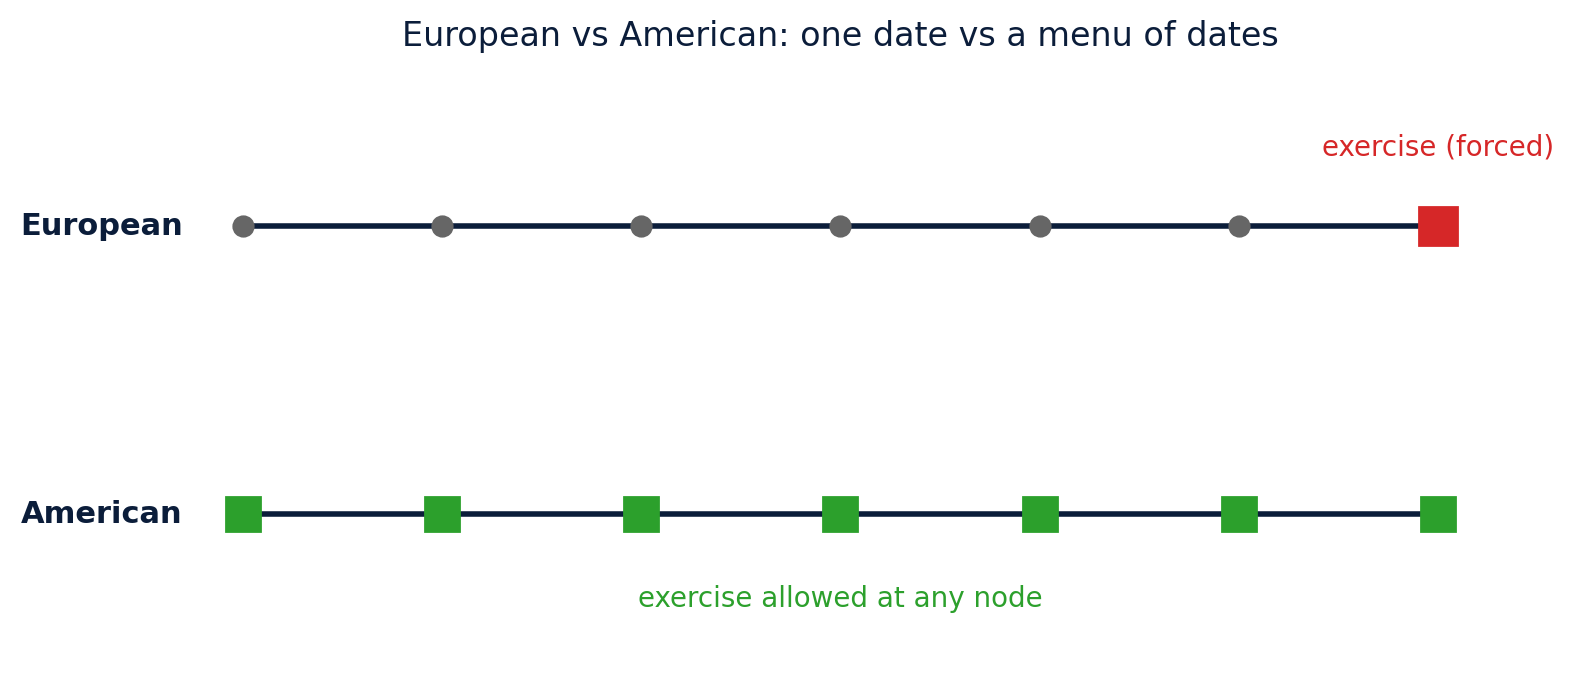
\includegraphics[keepaspectratio]{figures/ch04-eu-vs-am-timeline.png}}
\caption{European vs American timeline: a European has one cash-flow
date; an American offers a menu of dates, with the buyer choosing.}
\end{figure}

\begin{figure}
\centering
\pandocbounded{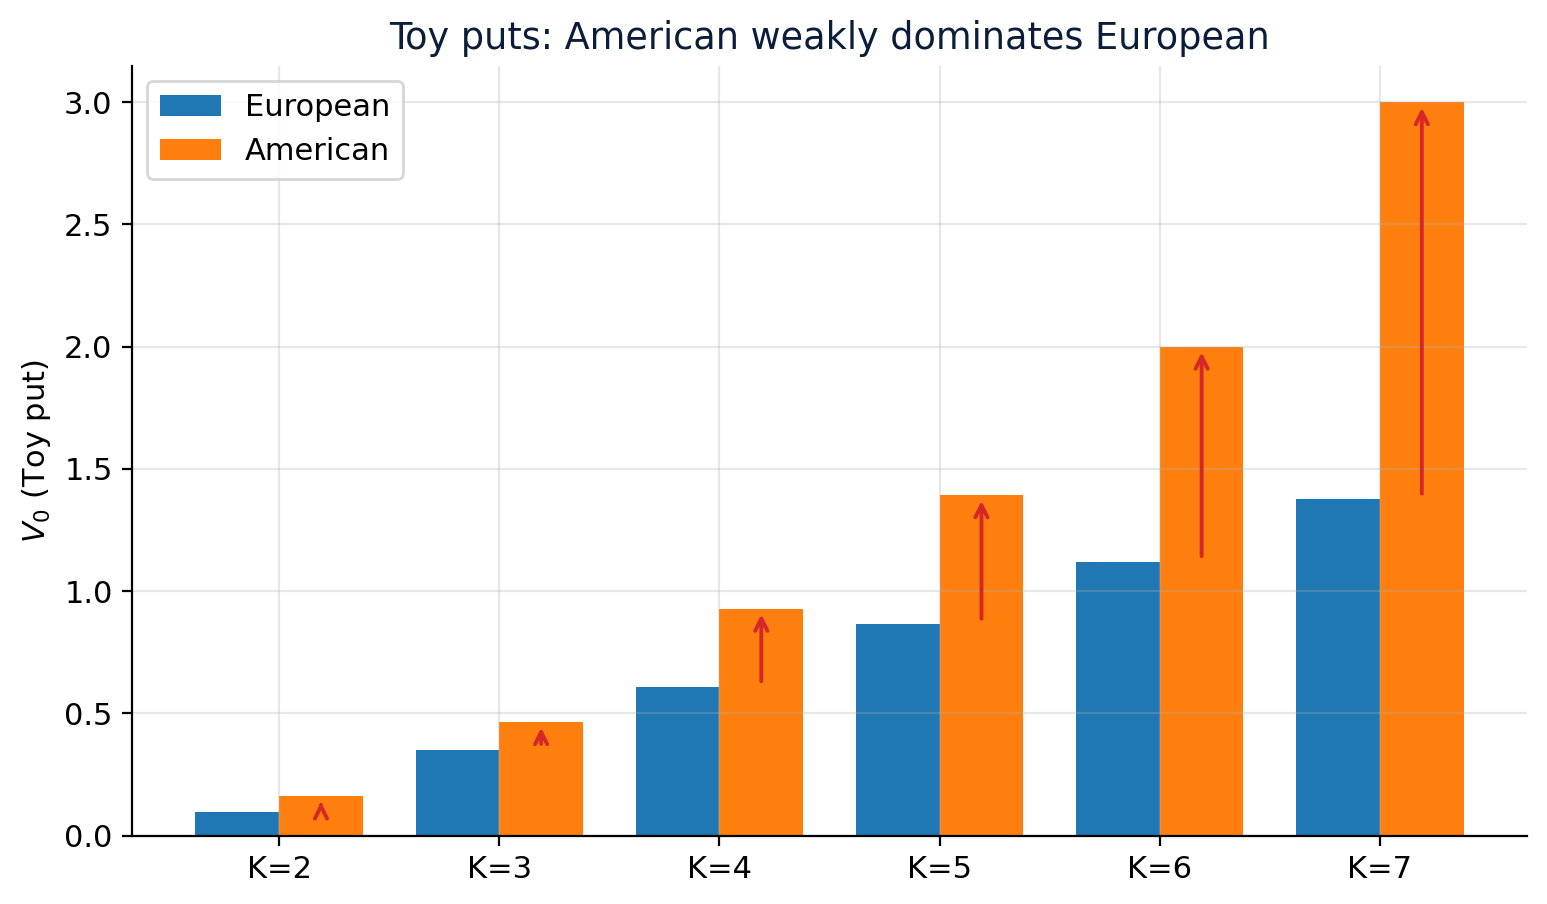
\includegraphics[keepaspectratio]{figures/ch04-eu-vs-am-bars.png}}
\caption{Toy puts at strikes \(K = 2, \dots, 7\): side-by-side European
and American prices. The American price always weakly dominates and the
gap is the early-exercise premium.}
\end{figure}

\subsection{4.1.4 Table}\label{table-16}

\textbf{Table 4.1.} ST toy put comparison of three stopping rules
(above), and analogous numbers for the realistic put \(K = 100\) over
\(n = 3\):

{\def\LTcaptype{none} % do not increment counter
\begin{table}[H]
\centering
\begin{tabular}{|l|l|r|}
\toprule
lattice & rule & \(V_0\) \\
\midrule



ST toy, \(K=5\) & \(\tau \equiv 0\) & \(1.000\) \\
ST toy, \(K=5\) & \(\tau \equiv 2\) (European) & \(0.960\) \\
ST toy, \(K=5\) & \(\tau^*\) (American) & \(1.360\) \\
Realistic, \(K=100\) & \(\tau \equiv 0\) & \(0.000\) \\
Realistic, \(K=100\) & \(\tau \equiv 3\) (European) & \(4.593\) \\
Realistic, \(K=100\) & \(\tau^*\) (American) & \(4.907\) \\
\bottomrule
\end{tabular}
\end{table}
}

The European is one of the strategies the American buyer could choose;
she chooses better.

\begin{center}\rule{0.5\linewidth}{0.5pt}\end{center}

\section{§4.2 Stopping times and the buyer's
problem}\label{stopping-times-and-the-buyers-problem}

\textbf{Punchline.} The American buyer's problem is

\[V_0^{\text{Am}} \;=\; \sup_{\tau \in \mathcal{T}_{0,n}} \tilde{\mathbb{E}}\!\left[\beta^\tau\, g(S_\tau)\right].\]

Stopping times are decision rules computable from past observations only
--- \textbf{no future peeking}. The whole chapter is about how to
compute this sup.

\textbf{Intuition.} Imagine you're walking the binomial tree node by
node. At each node you must decide \emph{yes-exercise} or
\emph{no-continue}, knowing only the path so far. You may carry any
deterministic logic with you --- ``exercise the first time \(S\) drops
below \(3\)'', ``exercise on the third up-move'', ``exercise on day
\(5\) no matter what'' --- anything but ``exercise on the path's
eventual minimum.'' The latter is forbidden because at the time you'd
commit to it, you can't see the future.

\subsection{4.2.1 Reminder: what is a stopping
time?}\label{reminder-what-is-a-stopping-time}

Recall from Ch 3, §3.4: \(\tau: \Omega \to \{0, 1, \dots, n, \infty\}\)
is a \textbf{stopping time} with respect to the filtration
\(\{\mathcal F_k\}\) if

\[\{\tau \le k\} \in \mathcal F_k \quad \text{for every } k \in \{0, 1, \dots, n\}.\]

Equivalently, for each path \(\omega\), the value \(\tau(\omega)\) is
decided as soon as the path enters \(\mathcal F_k\) --- that is, when
the first \(k\) tosses are revealed. A coin-toss path
\(\omega = (\omega_1, \omega_2, \dots, \omega_n)\) at time \(k\) has
revealed \((\omega_1, \dots, \omega_k)\).

\textbf{Examples that \emph{are} stopping times} (no peeking):

\begin{itemize}
\tightlist
\item
  \(\tau \equiv c\) (constant time).
\item
  \(\tau = \min\{k \ge 0 : S_k \le L\}\) (first hitting of level \(L\)
  below).
\item
  \(\tau = \min\{k \ge 0 : g(S_k) \ge V_k\}\) (first time intrinsic
  touches Snell envelope --- see §4.4).
\item
  \(\tau = n \wedge \min\{k : \text{condition}_k\}\) (any hitting time
  capped at maturity).
\end{itemize}

\textbf{Examples that are \emph{not} stopping times}:

\begin{itemize}
\tightlist
\item
  \(\tau =\) the index \(k\) where \(S_k\) attains its global maximum
  over \(k = 0, \dots, n\). (Requires future.)
\item
  \(\tau =\) ``exercise one step before the price crashes''. (Requires
  future.)
\item
  \(\tau =\) ``exercise at the average of high and low days''. (Average
  of future days requires future.)
\end{itemize}

\subsection{4.2.2 The buyer's
optimisation}\label{the-buyers-optimisation}

We want to compute

\[\sup_{\tau \in \mathcal{T}_{0,n}} \tilde{\mathbb{E}}\!\left[\beta^\tau\, g(S_\tau)\right].\]

The supremum is over a finite set: with \(n\) steps and \(2^n\) paths,
there are only finitely many possible \(\tau\)'s. In principle one could
enumerate them all and pick the best. We will instead derive a recursion
(the Snell envelope, §4.3) that solves this without enumeration.

Some sanity checks before we get there.

\textbf{Example 4.2.1 (ST put \(K = 5\), hitting time rule).} Let
\(\tau_a = \min\{k \ge 0 : S_k \le 2\}\) --- first hit of the level
\(2\). With the toy lattice \(S_0 = 4\):

\begin{itemize}
\tightlist
\item
  Path \(HH\): \(S_1 = 8, S_2 = 16\) --- never hits.
  \(\tau_a = \infty\), payoff \(0\) (convention).
\item
  Path \(HT\): \(S_1 = 8, S_2 = 4\) --- never hits. \(\tau_a = \infty\),
  payoff \(0\).
\item
  Path \(TH\): \(S_1 = 2\) --- hits at \(k = 1\). \(\tau_a = 1\), payoff
  \(g(2) = 3\).
\item
  Path \(TT\): \(S_1 = 2\) --- hits at \(k = 1\). \(\tau_a = 1\), payoff
  \(g(2) = 3\).
\end{itemize}

To use this consistently across the no-hit paths we must extend \(g\) at
\(\tau = \infty\) to give \(0\). Then

\[\tilde{\mathbb{E}}[\beta^{\tau_a} g(S_{\tau_a})] = \tfrac{1}{2}\!\cdot\!\beta\!\cdot\!3 + \tfrac{1}{2}\!\cdot\!0 = \tfrac{1}{2}\!\cdot\!\tfrac{4}{5}\!\cdot\!3 = 1.20.\]

(We averaged over \(\tilde p = 1/2\): \(P(\text{first toss} = T) = 1/2\)
gives payoff \(\beta \cdot 3\); \(P(\text{first toss} = H) = 1/2\) gives
\(0\).)

So \(\tau_a\) achieves \(1.20\). Not bad --- better than the European
\(0.96\), worse than the actual American \(1.36\).

\textbf{Example 4.2.2 (the rule ``exercise at the path-minimum'').}
Define \(\tau_{\min} := \mathrm{arg\,min}_k S_k\). On the toy lattice,
on path \(HH\) the minimum is \(S_0 = 4\) at \(k = 0\); on path \(HT\)
the minimum is \(S_2 = 4\) at \(k = 2\); on path \(TH\) the minimum is
\(S_1 = 2\); on path \(TT\) the minimum is \(S_2 = 1\). At \(k = 0\)
both paths \(HH\) and \(HT\) start identically (they share the prefix),
but \(\tau_{\min}\) would assign them different values (\(0\) vs \(2\)).
That contradicts the requirement that \(\tau\) be decidable from
\(\mathcal F_0\) alone (which contains only the trivial information at
\(k = 0\)). \textbf{Not a stopping time}.

\textbf{Example 4.2.3 (barrier hitting time on realistic).} Define
\(\tau_B = \min\{k : S_k \ge 108\}\) on the realistic lattice
(\(n = 3\)). Enumerate paths:

{\def\LTcaptype{none} % do not increment counter
\begin{table}[H]
\centering
\begin{tabular}{|l|r|r|r|c|r|}
\toprule
path & \(S_1\) & \(S_2\) & \(S_3\) & \(\tau_B\) & \(g_{\text{call}}\) \\
\midrule



\(HHH\) & \(110\) & \(121\) & \(133.1\) & \(1\) & \(10\) \\
\(HHT\) & \(110\) & \(121\) & \(108.9\) & \(1\) & \(10\) \\
\(HTH\) & \(110\) & \(99\) & \(108.9\) & \(1\) & \(10\) \\
\(HTT\) & \(110\) & \(99\) & \(89.1\) & \(1\) & \(10\) \\
\(THH\) & \(90\) & \(99\) & \(108.9\) & \(3\) & \(8.90\) \\
\(THT\) & \(90\) & \(99\) & \(89.1\) & \(\infty\) & \(0\) \\
\(TTH\) & \(90\) & \(81\) & \(89.1\) & \(\infty\) & \(0\) \\
\(TTT\) & \(90\) & \(81\) & \(72.9\) & \(\infty\) & \(0\) \\
\bottomrule
\end{tabular}
\end{table}
}

\emph{Payoff column:} \(g_{\text{call}}(S_{\tau_B})\) at strike
\(K = 100\) --- zero when \(\tau_B = \infty\) (barrier never hit).

Under \(\tilde p = 0.6\), the probability of each \(\omega\) is
\(0.6^{\#H}\cdot 0.4^{\#T}\). Discounted expected payoff:

\[\begin{aligned}
\tilde{\mathbb{E}}[\beta^{\tau_B} g(S_{\tau_B})] &= \beta\cdot 10\cdot \tilde{\mathbb{P}}(\text{first toss }H) + \beta^3 \cdot 8.9 \cdot \tilde{\mathbb{P}}(THH) \\
&= \tfrac{1}{1.02}\!\cdot 10\!\cdot 0.6 + \tfrac{1}{1.061208}\!\cdot 8.9\!\cdot 0.144 \\
&\approx 5.882 + 1.208 = 7.090.
\end{aligned}\]

Quite a bit less than the European call \(10.360\). The hitting-time
rule for the call is \emph{suboptimal} --- natural intuition: for a
non-dividend call, the right rule is to \emph{not} exercise early at
all.

\textbf{Example 4.2.4 (ST put \(K=5\) --- comparing three rules).} On
the toy lattice, three rules:

\begin{itemize}
\tightlist
\item
  \(\tau_a \equiv 0\): payoff \(g(4) = 1\). Discounted expectation =
  \(1.00\).
\item
  \(\tau_b = \min\{k : \omega_k = T\}\) (first down), with the
  convention \(\tau_b = n\) if no \(T\) ever shows. On the four paths:
\end{itemize}

{\def\LTcaptype{none} % do not increment counter
\begin{table}[H]
\centering
\begin{tabular}{|l|r|c|r|r|r|}
\toprule
path & path \(\tilde{\mathbb{P}}\) & \(\tau_b\) & \(S_{\tau_b}\) & \(g(S_{\tau_b})\) & \(\beta^{\tau_b} g\) \\
\midrule



HH & \(1/4\) & \(2\) & \(16\) & \(0\) & \(0\) \\
HT & \(1/4\) & \(2\) & \(4\) & \(1\) & \(0.640\) \\
TH & \(1/4\) & \(1\) & \(2\) & \(3\) & \(2.400\) \\
TT & \(1/4\) & \(1\) & \(2\) & \(3\) & \(2.400\) \\
\bottomrule
\end{tabular}
\end{table}
}

\(\tilde{\mathbb{E}}[\beta^{\tau_b} g] = (0 + 0.64 + 2.40 + 2.40)/4 = 1.36\).

That's \textbf{exactly} the American value. We have stumbled onto
\(\tau^*\)! The rule ``stop at the first down'' is optimal for this
contract on this lattice. Section 4.4 will derive it systematically.

\begin{itemize}
\tightlist
\item
  \(\tau_c \equiv 2\) (always wait to maturity): this is the European,
  \(0.96\).
\end{itemize}

\textbf{Example 4.2.5 (constant-time stop, realistic put).} With
\(K = 100\), \(n = 3\), consider \(\tau \equiv 1\):

\[\tilde{\mathbb{E}}[\beta\cdot g(S_1)] = \tfrac{1}{1.02}\!\left[0.6\cdot 0 + 0.4 \cdot 10\right] = \tfrac{4}{1.02} \approx 3.922.\]

A constant-time stop gives \(3.922\) --- less than both European
\(4.593\) and American \(4.907\).

\subsection{4.2.3 Why the supremum
exists}\label{why-the-supremum-exists}

There are only finitely many measurable stopping rules on a finite tree.
Each defines a number \(\tilde{\mathbb{E}}[\beta^\tau g(S_\tau)]\). The
sup over a finite set is attained --- there is an actual rule \(\tau^*\)
that achieves \(V_0^{\text{Am}}\), not merely a limit.

This is one of the great gifts of working in \emph{discrete} time. In
continuous time the same conclusion holds but requires technical
machinery (semi-continuity of expectations). In our setting it's just
``the max of finitely many numbers exists.''

\begin{figure}
\centering
\pandocbounded{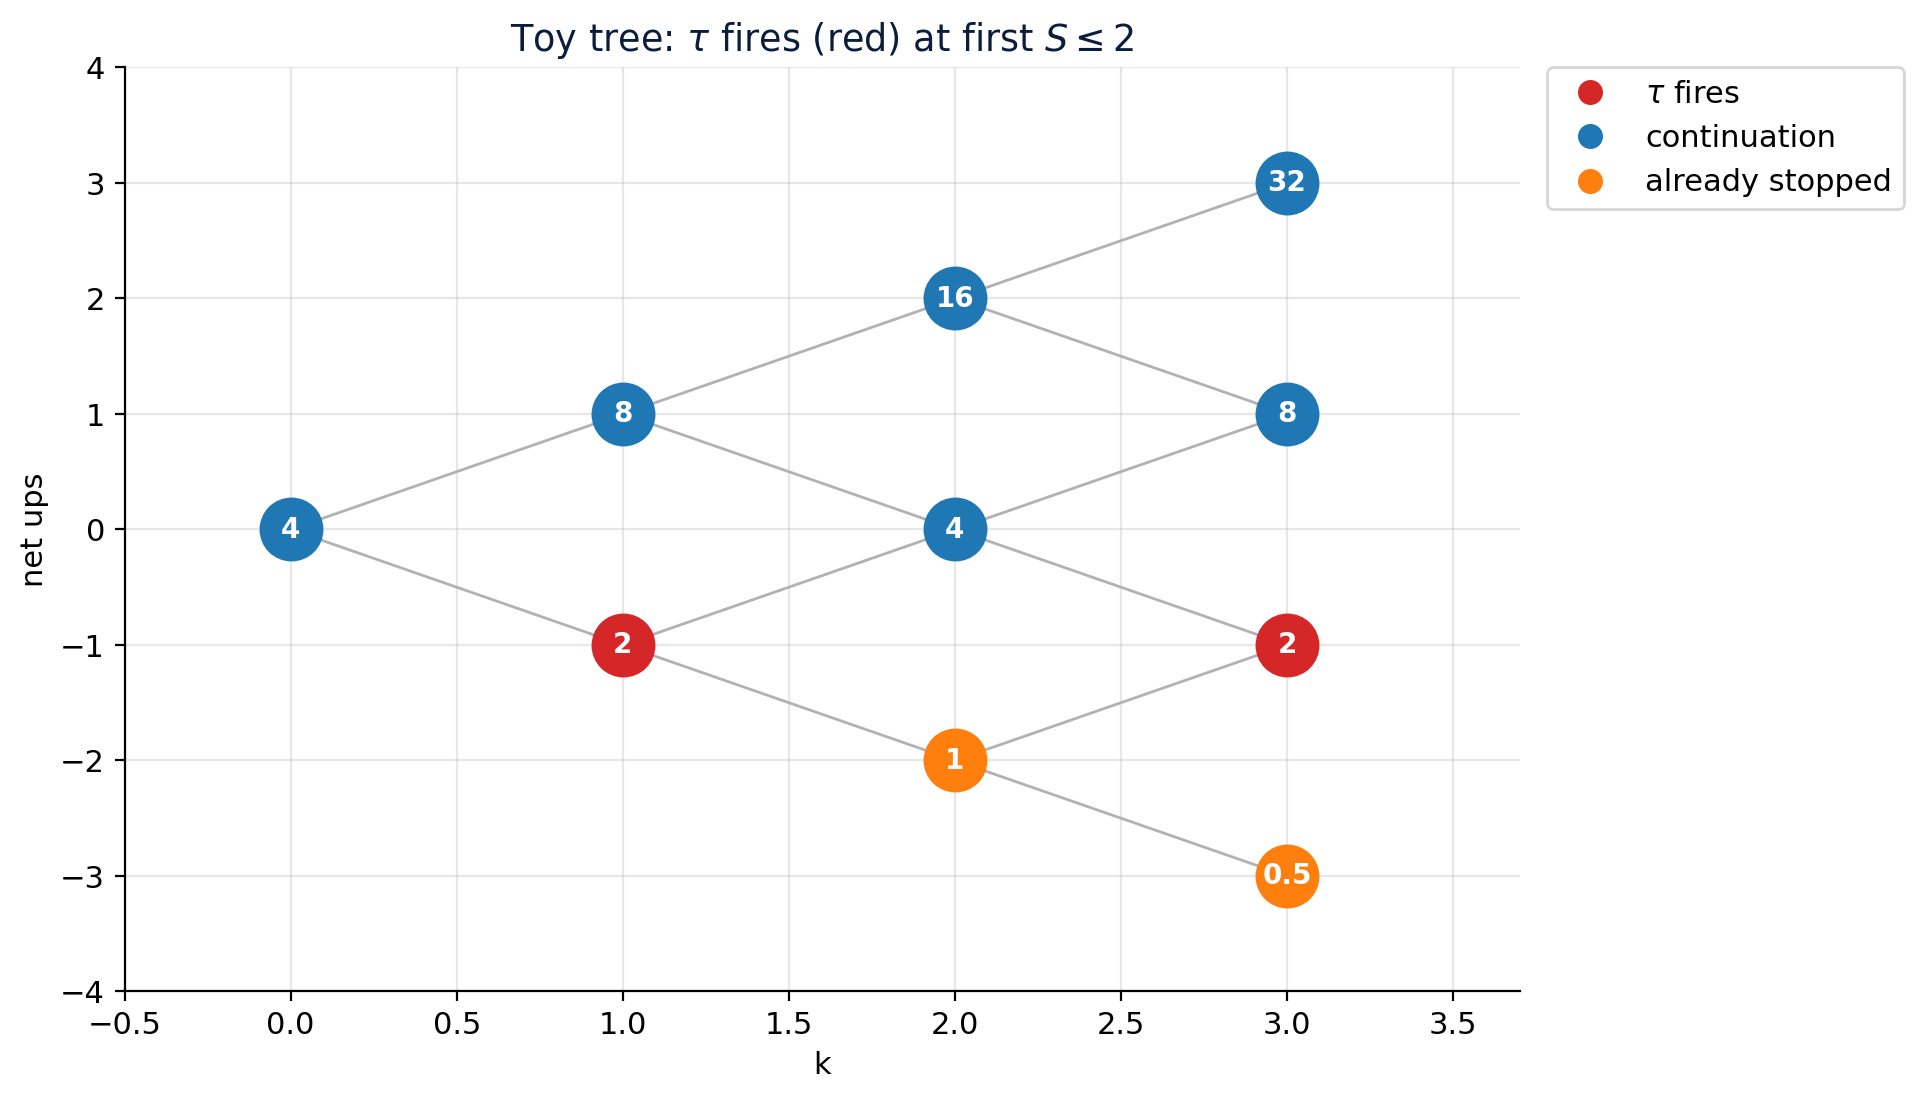
\includegraphics[keepaspectratio]{figures/ch04-tau-shaded.png}}
\caption{Toy ST tree with the rule ``stop at first \(S \le 2\)''
highlighted. Red nodes are where \(\tau\) actually fires; blue nodes are
continuation; orange would have stopped but the path already stopped
earlier.}
\end{figure}

\begin{figure}
\centering
\pandocbounded{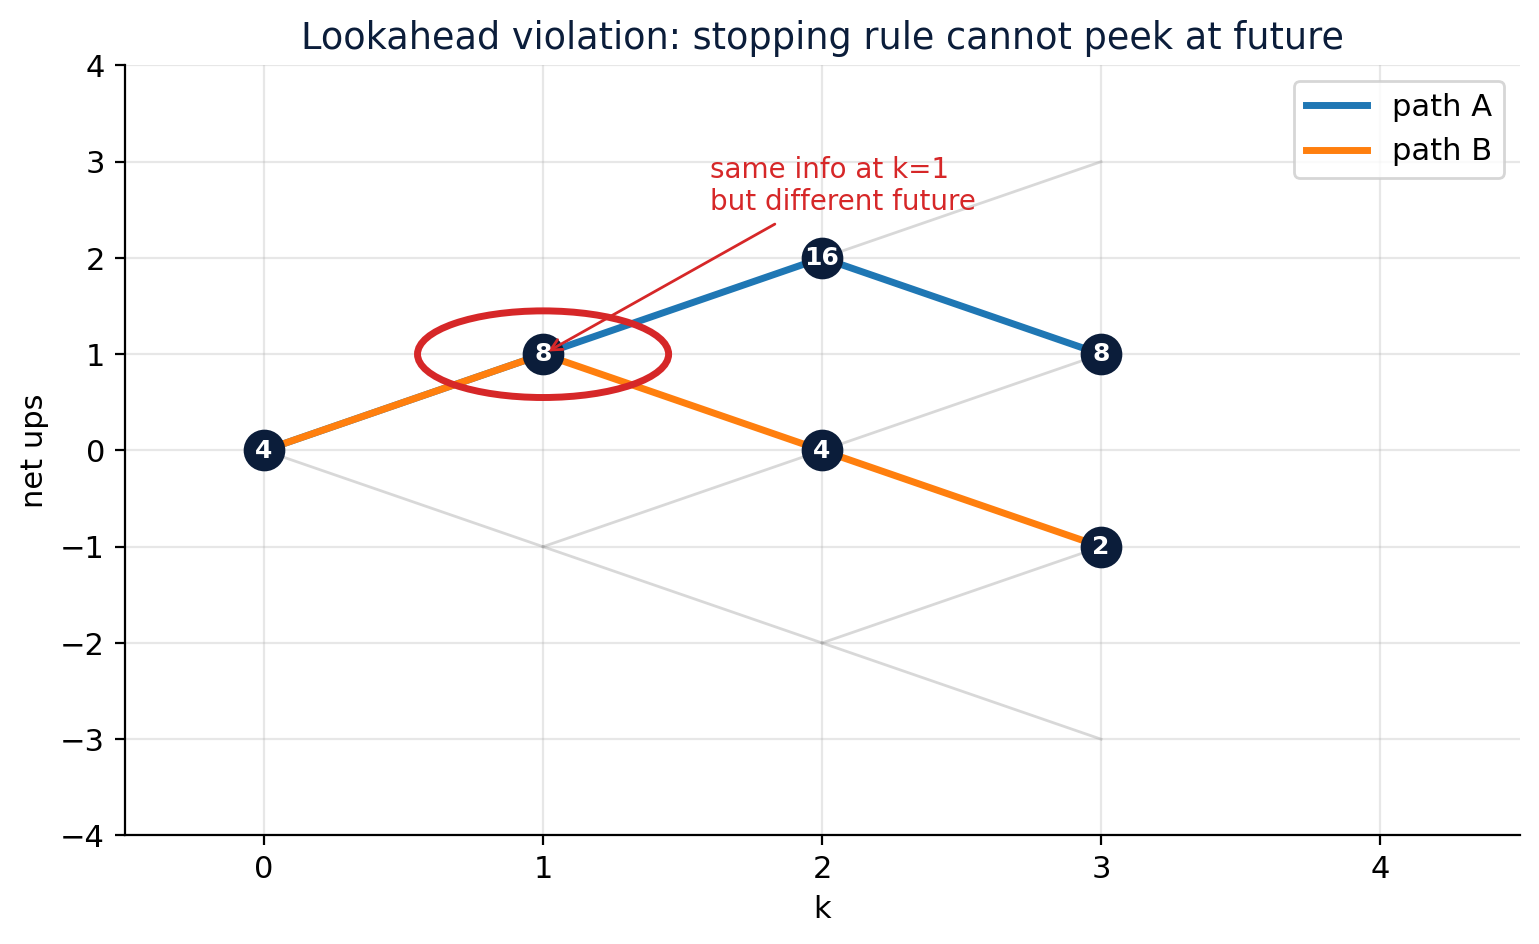
\includegraphics[keepaspectratio]{figures/ch04-lookahead-violation.png}}
\caption{Two paths sharing the same first step but ending differently
--- a rule that uses the future would treat them differently at \(k=1\),
in violation of the stopping-time definition.}
\end{figure}

\subsection{4.2.4 Table}\label{table-17}

\textbf{Table 4.2.} Five stopping rules on the ST put \(K=5\) with their
discounted expected payoffs:

{\def\LTcaptype{none} % do not increment counter
\begin{table}[H]
\centering
\begin{tabular}{|l|l|r|}
\toprule
rule & description & \(\tilde{\mathbb{E}}[\beta^\tau g]\) \\
\midrule



\(\tau \equiv 0\) & exercise now & \(1.00\) \\
\(\tau \equiv 1\) & exercise at \(k=1\) & \(1.20\) \\
\(\tau \equiv 2\) & European & \(0.96\) \\
\(\tau_a\) & first-touch level 2 & \(1.20\) \\
\(\tau_b\) & first down & \textbf{\(1.36\)} \\
\bottomrule
\end{tabular}
\end{table}
}

\emph{Definitions:} \(\tau_a = \min\{k : S_k \le 2\}\);
\(\tau_b = \min\{k : \omega_k = T\}\). The \(\tau \equiv 2\) rule
reduces to the European-style payoff at maturity.

The best of these is \(\tau_b\), attaining \(1.36 = V_0^{\text{Am}}\).

\begin{center}\rule{0.5\linewidth}{0.5pt}\end{center}

\section{§4.3 The Snell envelope}\label{the-snell-envelope}

\textbf{Punchline.} Define the buyer's value function by backward
induction:

\[\boxed{\;\begin{aligned}
V_n &:= g(S_n), \\
V_k &:= \max\!\Big\{g(S_k),\; \beta\, \tilde{\mathbb{E}}[V_{k+1}\mid \mathcal F_k]\Big\}\\
&\quad\text{for } k = n-1, n-2, \dots, 0.
\end{aligned}\;}\]

This process \(\{V_k\}\) is called the \textbf{Snell envelope} of the
discounted payoff. It is the smallest supermartingale that dominates the
intrinsic process. And \(V_0 = V_0^{\text{Am}}\).

\textbf{Intuition.} At every node the buyer compares two numbers: (i)
``exercise now and walk away with \(g(S_k)\)'', versus (ii) ``wait one
period --- the discounted expected value of holding is
\(\beta \tilde{\mathbb{E}}[V_{k+1}\mid \mathcal F_k]\)''. Whichever is
larger, that's \(V_k\). The recursion is just the principle that
\emph{the optimal first move is the optimal first move from where you'll
start tomorrow}, which is the entire content of \textbf{dynamic
programming}.

\subsection{4.3.1 Setup and the
recursion}\label{setup-and-the-recursion}

For a payoff process \(\{g_k\}_k\) on a filtered probability space, the
\textbf{Snell envelope} is the process \(\{V_k\}\) defined by

\[V_n = g_n, \qquad V_k = \max\big\{g_k,\, \beta\, \tilde{\mathbb{E}}[V_{k+1}\mid\mathcal F_k]\big\}.\]

In our setting \(g_k = g(S_k)\).

Three properties characterise \(V\) (and we'll verify each on examples):

\textbf{(i) Dominates the payoff.} \(V_k \ge g(S_k)\) at every node. By
construction.

\textbf{(ii) Discounted Snell envelope is a
\(\tilde{\mathbb{P}}\)-supermartingale.} Set
\(\tilde V_k := \beta^k V_k\) (discount to time-0 units). Then

\[\begin{aligned}
\tilde{\mathbb{E}}[\tilde V_{k+1}\mid\mathcal F_k] &= \beta^{k+1}\tilde{\mathbb{E}}[V_{k+1}\mid\mathcal F_k] \\
&= \beta^k\!\cdot\!\beta\!\tilde{\mathbb{E}}[V_{k+1}\mid\mathcal F_k] \le \beta^k\!\cdot V_k = \tilde V_k.
\end{aligned}\]

The inequality follows because
\(V_k \ge \beta\tilde{\mathbb{E}}[V_{k+1}\mid\mathcal F_k]\) by the max
in the recursion. So \(\tilde V\) is a supermartingale.

\textbf{(iii) Smallest supermartingale dominating
\(\tilde g_k := \beta^k g(S_k)\).} If \(\{U_k\}\) is any supermartingale
with \(U_k \ge \tilde g_k\) at every node, then \(U_k \ge \tilde V_k\).
We won't prove this in full generality (the proof is by backward
induction; details below). The minimality is conceptually important: any
``valid replication budget'' must be at least \(V_0\), so \(V_0\) is the
no-arbitrage \emph{floor}.

\subsection{\texorpdfstring{4.3.2 Worked example --- Toy put
\(K = 5\)}{4.3.2 Worked example --- Toy put K = 5}}\label{worked-example-toy-put-k-5}

This is the canonical example. We have
\(S_0 = 4, u = 2, d = 1/2, r = 1/4, \tilde p = 1/2\), \(\beta = 4/5\),
\(K = 5\).

\textbf{Step 1: terminal layer.} At \(k = 2\) the Snell envelope is the
intrinsic:

{\def\LTcaptype{none} % do not increment counter
\begin{table}[H]
\centering
\begin{tabular}{|c|r|r|}
\toprule
node \((2, j)\) & \(S_2\) & \(g(S_2) = V_2\) \\
\midrule



\((2, 0)\) TT & \(1\) & \(4\) \\
\((2, 1)\) HT or TH & \(4\) & \(1\) \\
\((2, 2)\) HH & \(16\) & \(0\) \\
\bottomrule
\end{tabular}
\end{table}
}

\textbf{Step 2: layer \(k = 1\).} For the \emph{up} node \((1, 1)\)
where \(S_1 = 8\):

\begin{itemize}
\tightlist
\item
  Intrinsic: \(g(8) = 0\).
\item
  Continuation:
  \(\beta\!\cdot\!\tilde{\mathbb{E}}[V_2\mid\mathcal F_1, \text{up}] = \tfrac{4}{5}\!\cdot\!\tfrac{1}{2}(V_2(HH) + V_2(HT)) = \tfrac{4}{5}\!\cdot\!\tfrac{1}{2}(0 + 1) = 0.40\).
\item
  \(V_1(1, 1) = \max\{0, 0.40\} = 0.40\) → \textbf{continue}.
\end{itemize}

For the \emph{down} node \((1, 0)\) where \(S_1 = 2\):

\begin{itemize}
\tightlist
\item
  Intrinsic: \(g(2) = 3\).
\item
  Continuation:
  \(\beta\!\cdot\!\tfrac{1}{2}(V_2(TH) + V_2(TT)) = \tfrac{4}{5}\!\cdot\!\tfrac{1}{2}(1 + 4) = 2.00\).
\item
  \(V_1(1, 0) = \max\{3, 2\} = 3\) → \textbf{exercise}.
\end{itemize}

\textbf{Step 3: root.}

\begin{itemize}
\tightlist
\item
  Intrinsic: \(g(4) = 1\).
\item
  Continuation:
  \(\beta\!\cdot\!\tfrac{1}{2}(V_1(1, 1) + V_1(1, 0)) = \tfrac{4}{5}\!\cdot\!\tfrac{1}{2}(0.40 + 3) = \tfrac{4}{5}\!\cdot 1.70 = 1.36\).
\item
  \(V_0 = \max\{1, 1.36\} = 1.36\) → \textbf{continue}.
\end{itemize}

\textbf{Result.} The American put price is \(V_0 = 1.36\).

{\def\LTcaptype{none} % do not increment counter
\begin{table}[H]
\centering
\begin{tabular}{|c|r|r|r|r|c|}
\toprule
node & \(S\) & \(g\) & cont. & \(V\) & regime \\
\midrule



\((0, 0)\) & \(\phantom{0}4\) & \(1\) & \(1.36\) & \(1.36\) &
\textbf{C} \\
\((1, 0)\) & \(\phantom{0}2\) & \(3\) & \(2.00\) & \(3.00\) &
\textbf{E} \\
\((1, 1)\) & \(\phantom{0}8\) & \(0\) & \(0.40\) & \(0.40\) & C \\
\((2, 0)\) & \(\phantom{0}1\) & \(4\) & & \(4.00\) & E \\
\((2, 1)\) & \(\phantom{0}4\) & \(1\) & & \(1.00\) & E \\
\((2, 2)\) & \(16\) & \(0\) & & \(0.00\) & term \\
\bottomrule
\end{tabular}
\end{table}
}

\emph{Column ``cont.''}
\(= \beta\tilde{\mathbb E}[V_{\cdot+1} \mid \mathcal F]\) --- the
discounted continuation value.

\emph{Legend.} C = continue (hold). E = exercise. term = terminal node,
no decision (continuation column blank). Blank in continuation column:
not computed (terminal node).*

\textbf{Example 4.3.1 (same, but \(K = 4\)).} Re-run with \(K = 4\):

\begin{itemize}
\tightlist
\item
  Terminal: \(V_2(0) = 3, V_2(1) = 0, V_2(2) = 0\).
\item
  \(V_1(1, 1) = \max\{0, \beta \cdot \tfrac{1}{2}(0+0)\} = 0\).
\item
  \(V_1(1, 0) = \max\{2, \beta\cdot \tfrac{1}{2}(0 + 3)\} = \max\{2, 1.20\} = 2\)
  → exercise.
\item
  \(V_0 = \max\{0, \beta\cdot\tfrac{1}{2}(0 + 2)\} = 0.80\).
\end{itemize}

So at \(K = 4\) the American put is \(0.80\). Notice that the \emph{up}
branch never has any value because the put is OTM and stays OTM.

\textbf{Example 4.3.2 (Toy, more strikes).}

{\def\LTcaptype{none} % do not increment counter
\begin{table}[H]
\centering
\begin{tabular}{|c|r|r|r|}
\toprule
\(K\) & \(V_0^{\text{Am}}\) & \(V_0^{\text{Eu}}\) & early-exercise
premium \\
\midrule



\(3\) & \(0.40\) & \(0.32\) & \(0.08\) \\
\(4\) & \(0.80\) & \(0.48\) & \(0.32\) \\
\(5\) & \(1.36\) & \(0.96\) & \(0.40\) \\
\(6\) & \(2.00\) & \(1.44\) & \(0.56\) \\
\(7\) & \(3.00\) & \(1.92\) & \(1.08\) \\
\bottomrule
\end{tabular}
\end{table}
}

The down-node \((1, 0)\) at \(S = 2\) has intrinsic \(K-2\) and
continuation \(\beta\cdot\tfrac{1}{2}(g(4)+g(1))\). For \(K \ge 3\) the
intrinsic strictly exceeds the continuation, so early exercise fires at
that node --- and the early-exercise premium grows with \(K\). For
\(K = 6, 7\) the root itself exercises immediately (\(V_0 = K - 4\)), as
you can check from the recursion.

\subsection{4.3.3 Realistic-lattice
example}\label{realistic-lattice-example}

\textbf{Example 4.3.3 (realistic put, \(K = 100\), \(n = 3\)).} With
\(S_0 = 100, u = 1.10, d = 0.90, r = 0.02, \tilde p = 0.6, \beta = 1/1.02 \approx 0.98039\).

Terminal prices and intrinsics (\(g(s) = (100-s)^+\)):

{\def\LTcaptype{none} % do not increment counter
\begin{table}[H]
\centering
\begin{tabular}{|l|r|r|}
\toprule
node & \(S_3\) & \(g\) \\
\midrule



HHH & \(133.10\) & \(0\) \\
HHT (×3) & \(108.90\) & \(0\) \\
HTT (×3) & \(89.10\) & \(10.90\) \\
TTT & \(72.90\) & \(27.10\) \\
\bottomrule
\end{tabular}
\end{table}
}

\textbf{Layer \(k = 2\).} \(S_2\) values: \(121, 99, 81\).

\begin{itemize}
\tightlist
\item
  Node \((2, 2)\), \(S = 121\): intrinsic \(0\). Continuation:
  \(\beta(\tilde p \cdot 0 + \tilde q\cdot 0) = 0\). \(V = 0\).
\item
  Node \((2, 1)\), \(S = 99\): intrinsic \(1\). Continuation:
  \(\beta(\tilde p\cdot 0 + \tilde q\cdot 10.9) = 0.98039\cdot 0.4\cdot 10.9 = 4.275\).
  \(V = 4.275\) → \textbf{continue}.
\item
  Node \((2, 0)\), \(S = 81\): intrinsic \(19\). Continuation:
  \(\beta(\tilde p\cdot 10.9 + \tilde q\cdot 27.1) = 0.98039\cdot(6.54 + 10.84) = 0.98039\cdot 17.38 = 17.038\).
  \(V = 19\) → \textbf{exercise}.
\end{itemize}

\textbf{Layer \(k = 1\).} \(S_1\) values: \(110, 90\).

\begin{itemize}
\tightlist
\item
  Node \((1, 1)\), \(S = 110\): intrinsic \(0\). Continuation:
  \(\beta(\tilde p\cdot 0 + \tilde q\cdot 4.275) = 0.98039\cdot 0.4\cdot 4.275 = 1.676\).
  \(V = 1.676\).
\item
  Node \((1, 0)\), \(S = 90\): intrinsic \(10\). Continuation:
  \(\beta(\tilde p\cdot 4.275 + \tilde q\cdot 19) = 0.98039\cdot(2.565 + 7.6) = 9.965\).
  \(V = 10\) → \textbf{exercise}, by a hair! The buyer captures the
  \(0.035\) early-exercise premium at this node.
\end{itemize}

\textbf{Root.} \(S_0 = 100\), intrinsic \(0\). Continuation:
\(\beta(\tilde p\cdot 1.676 + \tilde q\cdot 10) = 0.98039\cdot(1.006 + 4) = 4.907\).
\(V_0 = 4.907\).

{\def\LTcaptype{none} % do not increment counter
\begin{table}[H]
\centering
\begin{tabular}{|c|r|r|r|r|c|}
\toprule
node & \(S\) & \(g\) & cont & \(V\) & regime \\
\midrule



\((0,0)\) & \(100.00\) & \(\phantom{0}0.00\) & \(\phantom{0}4.907\) &
\(\phantom{0}4.907\) & C \\
\((1,1)\) & \(110.00\) & \(\phantom{0}0.00\) & \(\phantom{0}1.676\) &
\(\phantom{0}1.676\) & C \\
\((1,0)\) & \(\phantom{0}90.00\) & \(10.00\) & \(\phantom{0}9.965\) &
\(10.000\) & \textbf{E} \\
\((2,2)\) & \(121.00\) & \(\phantom{0}0.00\) & \(\phantom{0}0.000\) &
\(\phantom{0}0.000\) & term \\
\((2,1)\) & \(\phantom{0}99.00\) & \(\phantom{0}1.00\) &
\(\phantom{0}4.275\) & \(\phantom{0}4.275\) & C \\
\((2,0)\) & \(\phantom{0}81.00\) & \(19.00\) & \(17.038\) & \(19.000\) &
\textbf{E} \\
\((3,3)\) & \(133.10\) & \(\phantom{0}0.00\) & & \(\phantom{0}0.000\) &
term \\
\((3,2)\) & \(108.90\) & \(\phantom{0}0.00\) & & \(\phantom{0}0.000\) &
term \\
\((3,1)\) & \(\phantom{0}89.10\) & \(10.90\) & & \(10.900\) & term-E \\
\((3,0)\) & \(\phantom{0}72.90\) & \(27.10\) & & \(27.100\) & term-E \\
\bottomrule
\end{tabular}
\end{table}
}

\emph{Legend.} C = continue. E = exercise. term = terminal (no
continuation value). term-E = terminal in-the-money. Blank in cont
column: not computed at terminal nodes.*

\subsection{4.3.4 Supermartingale check}\label{supermartingale-check}

\textbf{Example 4.3.4 (verify the supermartingale property on the ST
toy).} With \(\tilde V_k = \beta^k V_k\) (discounted Snell), check
\(\tilde{\mathbb{E}}[\tilde V_{k+1}\mid\mathcal F_k] \le \tilde V_k\) at
each non-terminal node.

At root: \(\tilde V_0 = V_0 = 1.36\).
\(\tilde{\mathbb{E}}[\tilde V_1] = \beta\cdot\tfrac{1}{2}(V_1(1,1) + V_1(1,0)) = 0.8\cdot 0.5\cdot(0.40 + 3) = 1.36\).
\textbf{Equality} (the buyer would lose nothing by continuing one step).

At \((1, 0)\): \(\tilde V_1 = \beta\cdot 3 = 2.40\).
\(\tilde{\mathbb{E}}[\tilde V_2\mid\mathcal F_1, T] = \beta^2\cdot \tfrac{1}{2}(1 + 4) = 0.64\cdot 2.5 = 1.60\).
So
\(\tilde{\mathbb{E}}[\tilde V_2\mid \cdot] = 1.60 < \tilde V_1 = 2.40\).
\textbf{Strict drop} of \(0.80\). This is the source of the Doob
\emph{increasing process} below.

At \((1, 1)\): \(\tilde V_1 = \beta\cdot 0.40 = 0.32\).
\(\tilde{\mathbb{E}}[\tilde V_2 \mid \cdot] = \beta^2\cdot\tfrac{1}{2}(0 + 1) = 0.32\).
Equality.

So the supermartingale property holds with \emph{equality} at every node
except \((1, 0)\), where it strictly decreases. That node --- and only
that node --- is the node we \emph{would} exercise. The drop is the
\textbf{slack} \(A\) that Doob will isolate.

\subsection{4.3.5 Doob decomposition}\label{doob-decomposition}

\textbf{Theorem (Doob).} Every supermartingale \(X\) on a finite
filtration uniquely decomposes as

\[X_k = X_0 + M_k - A_k,\]

where \(M\) is a martingale with \(M_0 = 0\) and \(A\) is a
non-decreasing, \(\mathcal F_{k-1}\)-predictable process with
\(A_0 = 0\).

Apply to the discounted Snell envelope \(\tilde V_k = \beta^k V_k\): at
each step define the increment of \(A\) as the drop \emph{induced} by
the supermartingale property:

\[\Delta A_{k+1} := \tilde V_k - \tilde{\mathbb{E}}[\tilde V_{k+1}\mid\mathcal F_k] \;\ge\; 0,\]

and
\(M_{k+1} = M_k + \big(\tilde V_{k+1} - \tilde{\mathbb{E}}[\tilde V_{k+1}\mid\mathcal F_k]\big)\).
By construction, \(M\) has zero conditional drift (martingale) and \(A\)
is non-decreasing. The crucial fact: \(\Delta A_{k+1} > 0\) \textbf{iff}
the buyer would optimally exercise \emph{at} time \(k\) (the
supermartingale lost slack there).

\textbf{Example 4.3.5 (Doob columns, ST put \(K = 5\), path TT).}
Tabulate along the path \(\omega = TT\):

{\def\LTcaptype{none} % do not increment counter
\begin{table}[H]
\centering
\begin{tabular}{|c|r|r|r|r|r|r|}
\toprule
\(k\) & \(S_k\) & \(g\) & \(V_k\) & \(\tilde V_k\) & \(\Delta A_{k+1}\) & \(\Delta M_{k+1}\) \\
\midrule



\(0\) & \(4\) & \(1\) & \(1.36\) & \(1.36\) & \(0.00\) & \(+1.04\) \\
\(1\) & \(2\) & \(3\) & \(3.00\) & \(2.40\) & \(0.80\) & \(+0.96\) \\
\(2\) & \(1\) & \(4\) & \(4.00\) & \(2.56\) & & \\
\bottomrule
\end{tabular}
\end{table}
}

\emph{Columns:} \(\tilde V_k = \beta^k V_k\); \(\Delta M_{k+1}\) is the
martingale increment along path TT. Step-by-step: at \(k=0\),
\(\Delta M_1 = \tilde V_1 - \tilde{\mathbb{E}}[\tilde V_1] = 2.40 - 1.36 = +1.04\).
At \(k=1\),
\(\Delta M_2 = \tilde V_2 - \tilde{\mathbb{E}}[\tilde V_2 \mid \mathcal F_1, T] = 2.56 - 1.60 = +0.96\).

\emph{Blank: increments not defined at the terminal step (no \(A_3\) or
\(\Delta M_3\) in a 2-period model).}

So along path TT, \(A_0 = 0, A_1 = 0, A_2 = 0.80\). The increase happens
between \(k = 1\) and \(k = 2\) --- which records that \emph{at}
\(k = 1\) we should have stopped. And note this \(\Delta A\) aligns with
the exercise-region indicator at \((1, 0)\) from §4.3.4.

The discounted European-style payoff
\(\tilde{\mathbb{E}}[\beta^2 g(S_2)]\) is the
price-of-continuing-from-the-root, \(1.36\). The full optimal-stopping
pricing identity, stated cleanly in the next section, is
\(V_0 = \tilde{\mathbb{E}}[\beta^{\tau^*} g(S_{\tau^*})]\) for the right
stopping time \(\tau^*\).

\subsection{\texorpdfstring{4.3.6 Counter-example: a ``supermartingale''
that \emph{doesn't}
dominate}{4.3.6 Counter-example: a ``supermartingale'' that doesn't dominate}}\label{counter-example-a-supermartingale-that-doesnt-dominate}

\textbf{Example 4.3.6 (smaller supermartingale fails to dominate).} Try
setting \(U_k \equiv 0\) for all \(k\). Clearly \(U\) is a (trivial)
supermartingale --- constant zero, no positive drift required. But it
fails to dominate \(g\) because \(g(S_1 = 2) = 3 > 0\). Thus
\(U \not\ge g\), and \(U\) does not qualify. The Snell envelope is the
\emph{smallest} supermartingale dominating \(g\) --- anything smaller
either violates the supermartingale property or drops below the
intrinsic somewhere.

Try a sharper attempt: let \(W_0 = 1.20\), \(W_1 = 1.50\), \(W_2 = 3\)
at \((2,0)\), etc. Pick values, see if it's a supermartingale with
\(W \ge g\). It will fail somewhere --- by minimality, anywhere strictly
below \(V\) either breaks the supermartingale property or the
domination. Try it as an exercise.

\begin{figure}
\centering
\pandocbounded{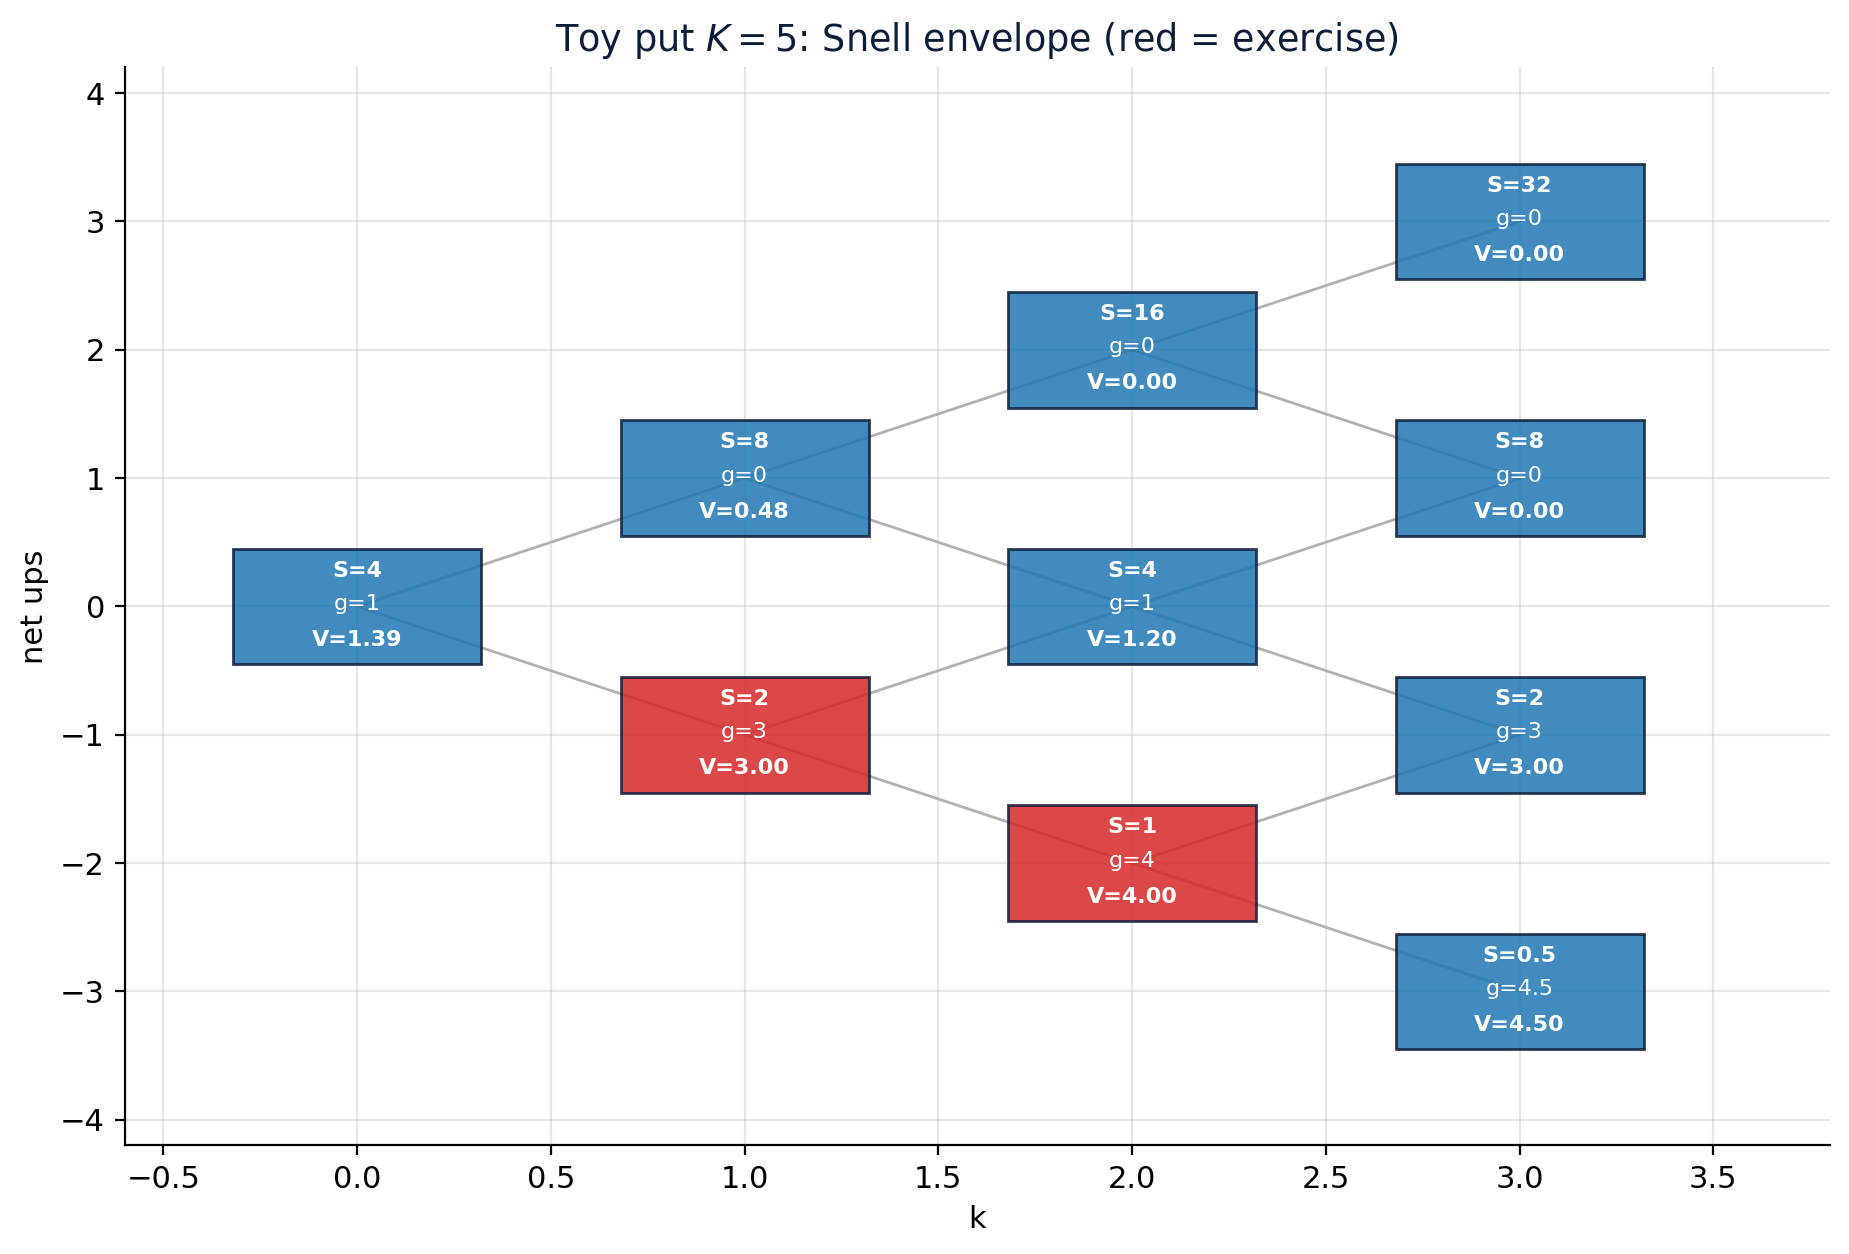
\includegraphics[keepaspectratio]{figures/ch04-snell-tree.png}}
\caption{ST put \(K=5\): the Snell envelope shown on the binomial tree.
At each node we display \(S\), intrinsic \(g\), and the envelope \(V\),
with red marking nodes where exercise is optimal.}
\end{figure}

\begin{figure}
\centering
\pandocbounded{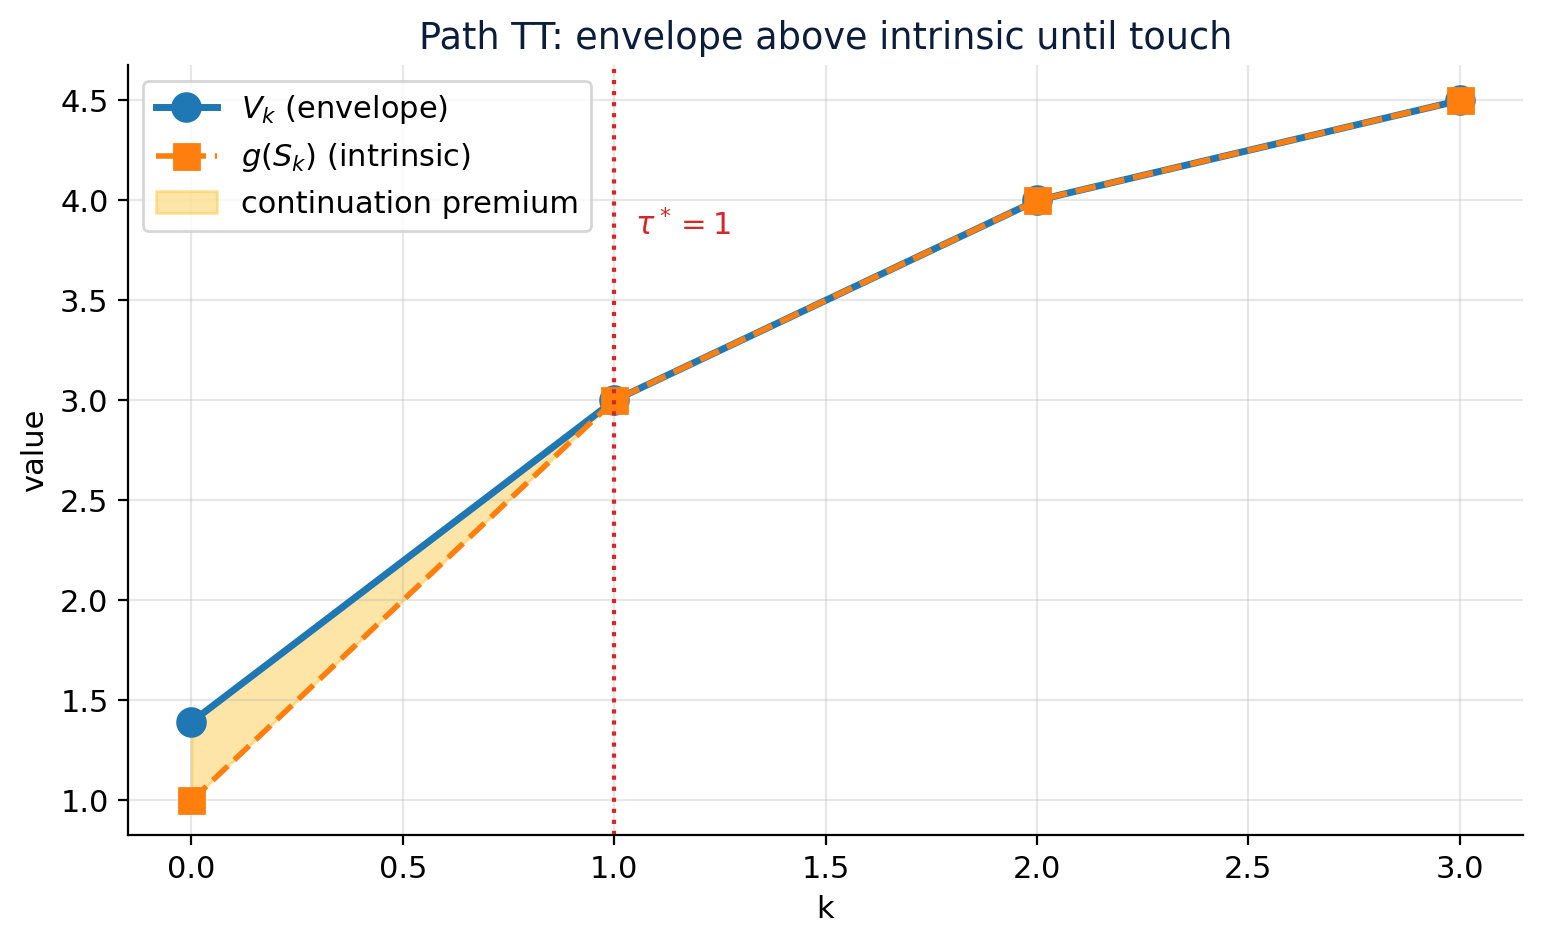
\includegraphics[keepaspectratio]{figures/ch04-V-vs-g.png}}
\caption{Path TT (down, down): \(V_k\) (blue) sits above the intrinsic
\(g(S_k)\) (orange) until it touches. The touch point is \(\tau^*\) and
the gold band is the continuation premium.}
\end{figure}

\begin{figure}
\centering
\pandocbounded{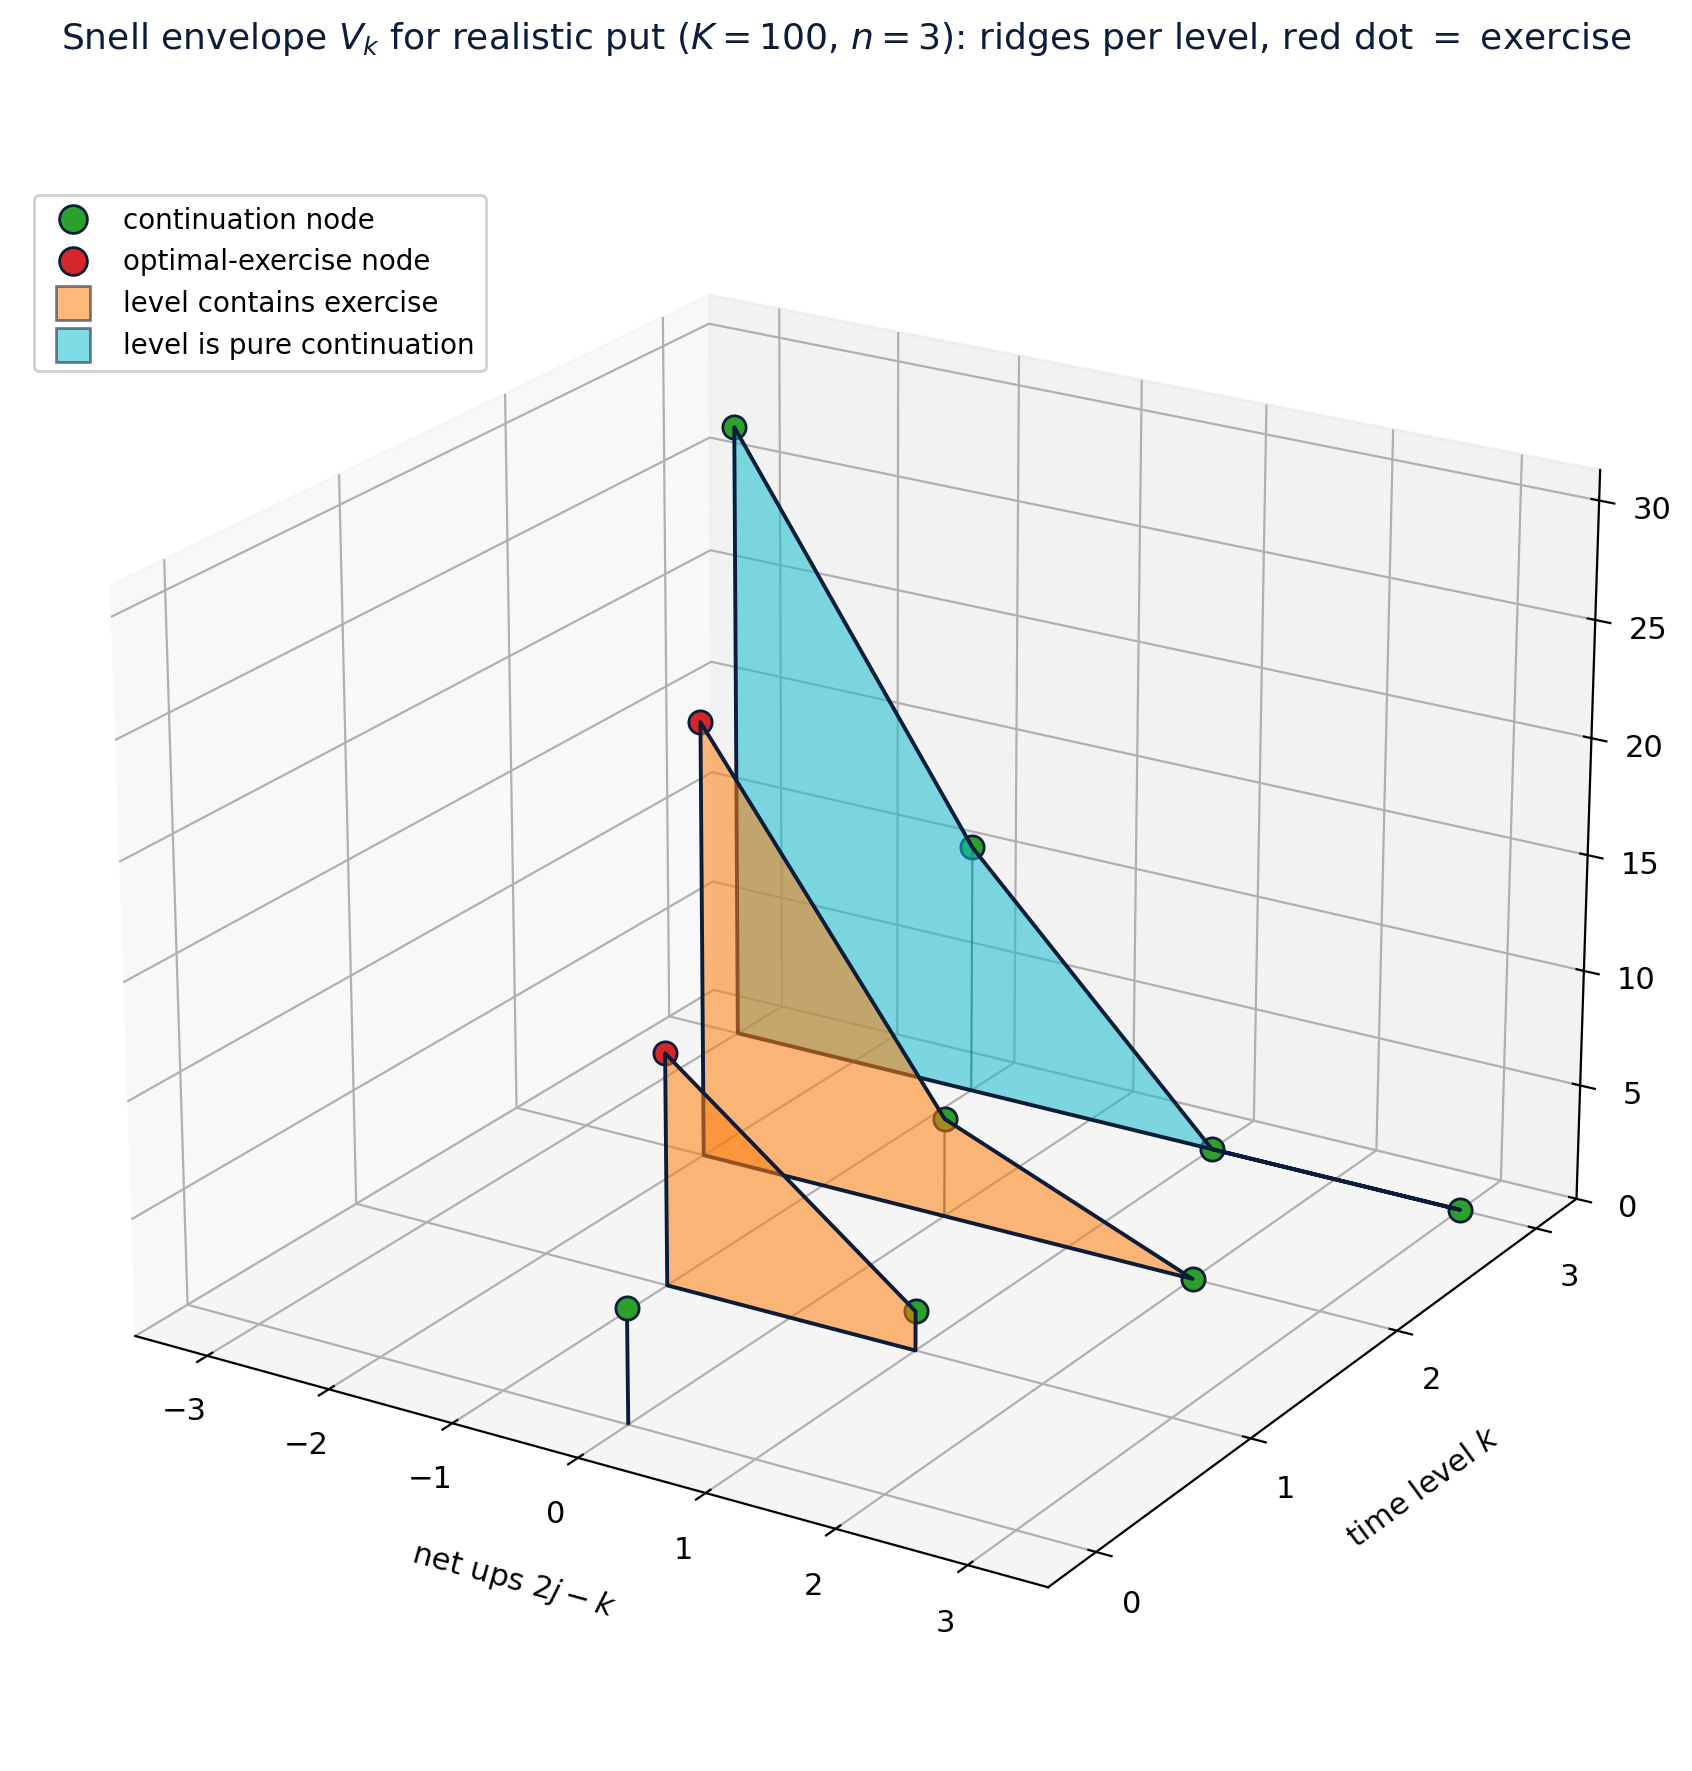
\includegraphics[keepaspectratio]{figures/ch04-Vk-3d.png}}
\caption{Realistic put \(K=100\), \(n=3\): Snell envelope \(V_k\) as 3-D
bars over \((k, 2j-k)\), coloured red where exercise is optimal and
green otherwise.}
\end{figure}

\subsection{4.3.7 Tables}\label{tables-6}

\textbf{Table 4.3.} ST put \(K = 5\) Snell envelope, every node.

(Reproduced from §4.3.2.)

\textbf{Table 4.4.} Doob decomposition columns for the ST put \(K = 5\)
on path TT.

(Reproduced from §4.3.5.)

\begin{center}\rule{0.5\linewidth}{0.5pt}\end{center}

\section{§4.4 Optimal exercise as a stopping
time}\label{optimal-exercise-as-a-stopping-time}

\textbf{Punchline.} The optimal stopping time is

\[\boxed{\ \tau^* \;:=\; \min\{k \in \{0, 1, \dots, n\} : V_k = g(S_k)\}.\ }\]

It is the \textbf{first time} the Snell envelope touches the intrinsic.
The stopped discounted Snell process \(\tilde V_{k \wedge \tau^*}\) is a
\emph{martingale} (not just a supermartingale). Equivalently,
\(V_0 = \tilde{\mathbb{E}}[\beta^{\tau^*} g(S_{\tau^*})]\) --- and no
stopping time achieves a higher discounted expected payoff.

\textbf{Intuition.} Walk the tree. As long as the envelope \(V_k\)
strictly exceeds the intrinsic \(g(S_k)\), you'd be a fool to exercise
--- waiting is worth more. The instant \(V_k\) drops to meet \(g(S_k)\),
waiting is no better; you may as well take the money. Stopping at that
instant is what makes the \emph{stopped} discounted process drift-free
(martingale), because beyond \(\tau^*\) the process is frozen and before
\(\tau^*\) the supermartingale property holds with equality (no slack
lost).

\subsection{\texorpdfstring{4.4.1 Why \(\tau^*\) is
optimal}{4.4.1 Why \textbackslash tau\^{}* is optimal}}\label{why-tau-is-optimal}

The argument is a two-line exercise once we have the Doob decomposition.

\textbf{Claim 1: \(\tau^*\) is a stopping time.} At time \(k\), the
indicator \(\{V_k = g(S_k)\}\) depends only on \((S_0, \dots, S_k)\),
hence on \(\mathcal F_k\). So
\(\{\tau^* \le k\} = \bigcup_{j \le k}\{V_j = g(S_j)\} \in \mathcal F_k\).
✓

\textbf{Claim 2: stopped discounted Snell envelope is a martingale.} The
supermartingale property of \(\tilde V\) holds with equality on the
\emph{continuation} region \(\{V_k > g(S_k)\}\) (no \(A\)-increment), by
construction of the recursion. After \(\tau^*\) the process is constant.
So \(\tilde V_{k \wedge \tau^*}\) has zero conditional drift everywhere.

\textbf{Claim 3:
\(V_0 = \tilde{\mathbb{E}}[\beta^{\tau^*} g(S_{\tau^*})]\).} Applying
the Optional Stopping Theorem (Ch 3, §3.6) to the \emph{martingale}
\(\tilde V_{k\wedge \tau^*}\):

\[\begin{aligned}
V_0 &= \tilde V_0 = \tilde{\mathbb{E}}[\tilde V_{n \wedge \tau^*}] = \tilde{\mathbb{E}}[\tilde V_{\tau^*}] \\
&= \tilde{\mathbb{E}}[\beta^{\tau^*} V_{\tau^*}] = \tilde{\mathbb{E}}[\beta^{\tau^*} g(S_{\tau^*})],
\end{aligned}\]

the last step because \(V_{\tau^*} = g(S_{\tau^*})\) by definition.

\textbf{Claim 4: no other \(\tau\) does better.} For any stopping time
\(\sigma \le n\):

\[\tilde{\mathbb{E}}[\beta^\sigma g(S_\sigma)] \le \tilde{\mathbb{E}}[\beta^\sigma V_\sigma] = \tilde{\mathbb{E}}[\tilde V_\sigma].\]

But \(\tilde V\) is a \emph{super}-martingale, so by OST
\(\tilde{\mathbb{E}}[\tilde V_\sigma] \le \tilde V_0 = V_0\).

Combining, \(V_0 = \sup_\tau \tilde{\mathbb{E}}[\beta^\tau g(S_\tau)]\)
and \(\tau^*\) achieves it.

\subsection{4.4.2 Worked example --- Toy put, every
path}\label{worked-example-toy-put-every-path}

\textbf{Example 4.4.1 (ST put \(K = 5\), \(\tau^*\) on every path).}
From §4.3.2 we have:

{\def\LTcaptype{none} % do not increment counter
\begin{table}[H]
\centering
\begin{tabular}{|c|r|r|c|}
\toprule
node & \(V\) & \(g\) & \(V = g\)? \\
\midrule



\((0, 0)\) & \(1.36\) & \(1\) & no \\
\((1, 0)\) T & \(3.00\) & \(3\) & \textbf{yes} \\
\((1, 1)\) H & \(0.40\) & \(0\) & no \\
\((2, 0)\) TT & \(4\) & \(4\) & term \\
\((2, 1)\) HT,TH & \(1\) & \(1\) & term \\
\((2, 2)\) HH & \(0\) & \(0\) & term \\
\bottomrule
\end{tabular}
\end{table}
}

\emph{Legend:} ``term'' = terminal node (trivially \(V = g\)).

Reading along each path:

{\def\LTcaptype{none} % do not increment counter
\begin{table}[H]
\centering
\begin{tabular}{|c|c|r|r|r|}
\toprule
path & \(\tau^*\) & \(S_{\tau^*}\) & \(g(S_{\tau^*})\) &
\(\beta^{\tau^*}g\) \\
\midrule



HH & \(2\) & \(16\) & \(0\) & \(0\) \\
HT & \(2\) & \(4\) & \(1\) & \(0.64\) \\
TH & \(1\) & \(2\) & \(3\) & \(2.40\) \\
TT & \(1\) & \(2\) & \(3\) & \(2.40\) \\
\bottomrule
\end{tabular}
\end{table}
}

Under \(\tilde{\mathbb{P}}\) each path has weight \(1/4\):

\[\tilde{\mathbb{E}}[\beta^{\tau^*} g] = \tfrac{1}{4}(0 + 0.64 + 2.40 + 2.40) = \tfrac{5.44}{4} = 1.36 \;=\; V_0. \checkmark\]

Path-by-path: ✓.

\textbf{Example 4.4.2 (suboptimal \(\tau \equiv 2\) --- show the gap).}
With \(\tau \equiv 2\) (the European stop):

\[\tilde{\mathbb{E}}[\beta^2 g(S_2)] = \beta^2\!\cdot\!\tfrac{1}{4}(0 + 1 + 1 + 4) = \tfrac{16}{25}\!\cdot\!\tfrac{6}{4} = 0.96.\]

Gap: \(V_0 - 0.96 = 0.40\). \textbf{And the gap is exactly the expected
\(A\)-increment along the path.} Specifically: along path TH and path TT
we should have stopped at \(k = 1\), not \(k = 2\). The gain we forfeit
by waiting is
\(\beta\cdot 3 - \beta^2\cdot \tfrac{1}{2}(1 + 4) = 2.40 - 1.60 = 0.80\)
on each ``down at \(k=1\)'' path. Average over the two such paths
(probability \(\tilde p \cdot \tilde q + \tilde q \cdot \tilde q = 1/2\)
in total): \(0.80 \cdot 1/2 = 0.40\). ✓ --- that's the gap.

\subsection{4.4.3 Realistic-lattice
example}\label{realistic-lattice-example-1}

\textbf{Example 4.4.3 (RL put \(K=100\), \(\tau^*\) on each path).} From
§4.3.3:

\begin{itemize}
\tightlist
\item
  \(V_{(1,0)} = g_{(1,0)} = 10\) → exercise at \(k=1\) along any path
  starting with \(T\).
\item
  \(V_{(2,0)} = g_{(2,0)} = 19\) → exercise at \(k=2\) along paths
  reaching \(S=81\). But: those paths \emph{also} go down at \(k=1\)
  (the only way to reach \((2,0)\) is TT) and thus would have exercised
  at \(k=1\) first. So \(\tau^* = 1\) on path TT.
\end{itemize}

Path-by-path. The labels HTT and THH share the same final stock price
but trigger early exercise at different times because the \textbf{path}
matters for \(\tau^* = \min\{k: V_k = g_k\}\). For path THH: at \(k=1\)
we are at \(S_1 = 90\), \(V = g = 10\), so \(\tau^* = 1\) and payoff is
\(\beta\cdot 10 = 9.804\). For path HTT: at \(k=1\) we are at
\(S_1 = 110\), \(V = 1.676\), \(g = 0\) --- don't exercise; at \(k=2\),
\(S_2 = 99\), \(V = 4.275\), \(g = 1\) --- don't exercise; at \(k=3\),
\(S_3 = 89.10\), \(g = 10.90\) --- exercise. So \(\tau^* = 3\) on path
HTT.

Path enumeration:

{\def\LTcaptype{none} % do not increment counter
\begin{table}[H]
\centering
\begin{tabular}{|l|r|c|r|r|r|r|}
\toprule
path & \(\tilde{\mathbb{P}}\) & \(\tau^*\) & \(S_{\tau^*}\) & \(g\) & \(\beta^{\tau^*}g\) & weighted \\
\midrule



HHH & \(0.216\) & n/a & \(133.10\) & \(0\) & \(0\) & \(0\) \\
HHT & \(0.144\) & n/a & \(108.90\) & \(0\) & \(0\) & \(0\) \\
HTH & \(0.144\) & n/a & \(108.90\) & \(0\) & \(0\) & \(0\) \\
HTT & \(0.096\) & \(3\) & \(89.10\) & \(10.90\) & \(10.272\) &
\(0.986\) \\
THH & \(0.144\) & \(1\) & \(90\) & \(10\) & \(9.804\) & \(1.412\) \\
THT & \(0.096\) & \(1\) & \(90\) & \(10\) & \(9.804\) & \(0.941\) \\
TTH & \(0.096\) & \(1\) & \(90\) & \(10\) & \(9.804\) & \(0.941\) \\
TTT & \(0.064\) & \(1\) & \(90\) & \(10\) & \(9.804\) & \(0.627\) \\
\bottomrule
\end{tabular}
\end{table}
}

Sum: \(0 + 0 + 0 + 0.986 + 1.412 + 0.941 + 0.941 + 0.627 = 4.907\).
Match. ✓ --- exactly the \(V_0\) we computed in §4.3.3.

\subsection{\texorpdfstring{4.4.4 Largest optimal stopping time
\(\tau^{\max}\)}{4.4.4 Largest optimal stopping time \textbackslash tau\^{}\{\textbackslash max\}}}\label{largest-optimal-stopping-time-taumax}

There is also a \emph{latest} stopping time that's still optimal:

\[\tau^{\max} := \min\{k : \Delta A_{k+1} > 0\}.\]

That is, \(\tau^{\max}\) is the first time the supermartingale would
strictly lose slack on the \emph{next} step. Any stopping time between
\(\tau^*\) and \(\tau^{\max}\) achieves the same expected payoff.

\textbf{Example 4.4.4 (ST put \(K = 5\), \(\tau^{\max}\)).} From the
Doob check in §4.3.4: the only node where \(\tilde V\) strictly
decreases is \((1, 0)\). So \(\Delta A_2 > 0\) on path TT and TH, namely
the increment happens between \(k=1\) and \(k=2\). Therefore
\(\tau^{\max} = 1\) on those paths (the latest step before slack
disappears), and \(\tau^{\max} = 2\) on the H-first paths (no slack ever
lost; you may as well wait). On H-first paths \(\tau^* = 2\) as well, so
they coincide.

\textbf{Example 4.4.5 (a case where \(\tau^* < \tau^{\max}\) strictly).}
Construct a contrived 3-step put with parameters such that exercise is
\emph{equally} attractive at \(k = 1\) and \(k = 2\) on the same path.
Imagine \(V_1 = g_1\) at \((1, 0)\) \emph{and} \(V_2 = g_2\) at the
down-down node with \(\Delta A_2 = 0\). Then \(\tau^* = 1\) (first
touch), \(\tau^{\max} = 2\) (latest touch before slack ends). Both
achieve \(V_0\).

This is more than a curiosity: in practice the boundary
\(\{V_k = g_k\}\) is \emph{fat}, and traders often distinguish ``early
exercise might be optimal'' from ``early exercise is \textbf{forced} to
be optimal''. The latter is \(\tau^{\max}\).

\begin{figure}
\centering
\pandocbounded{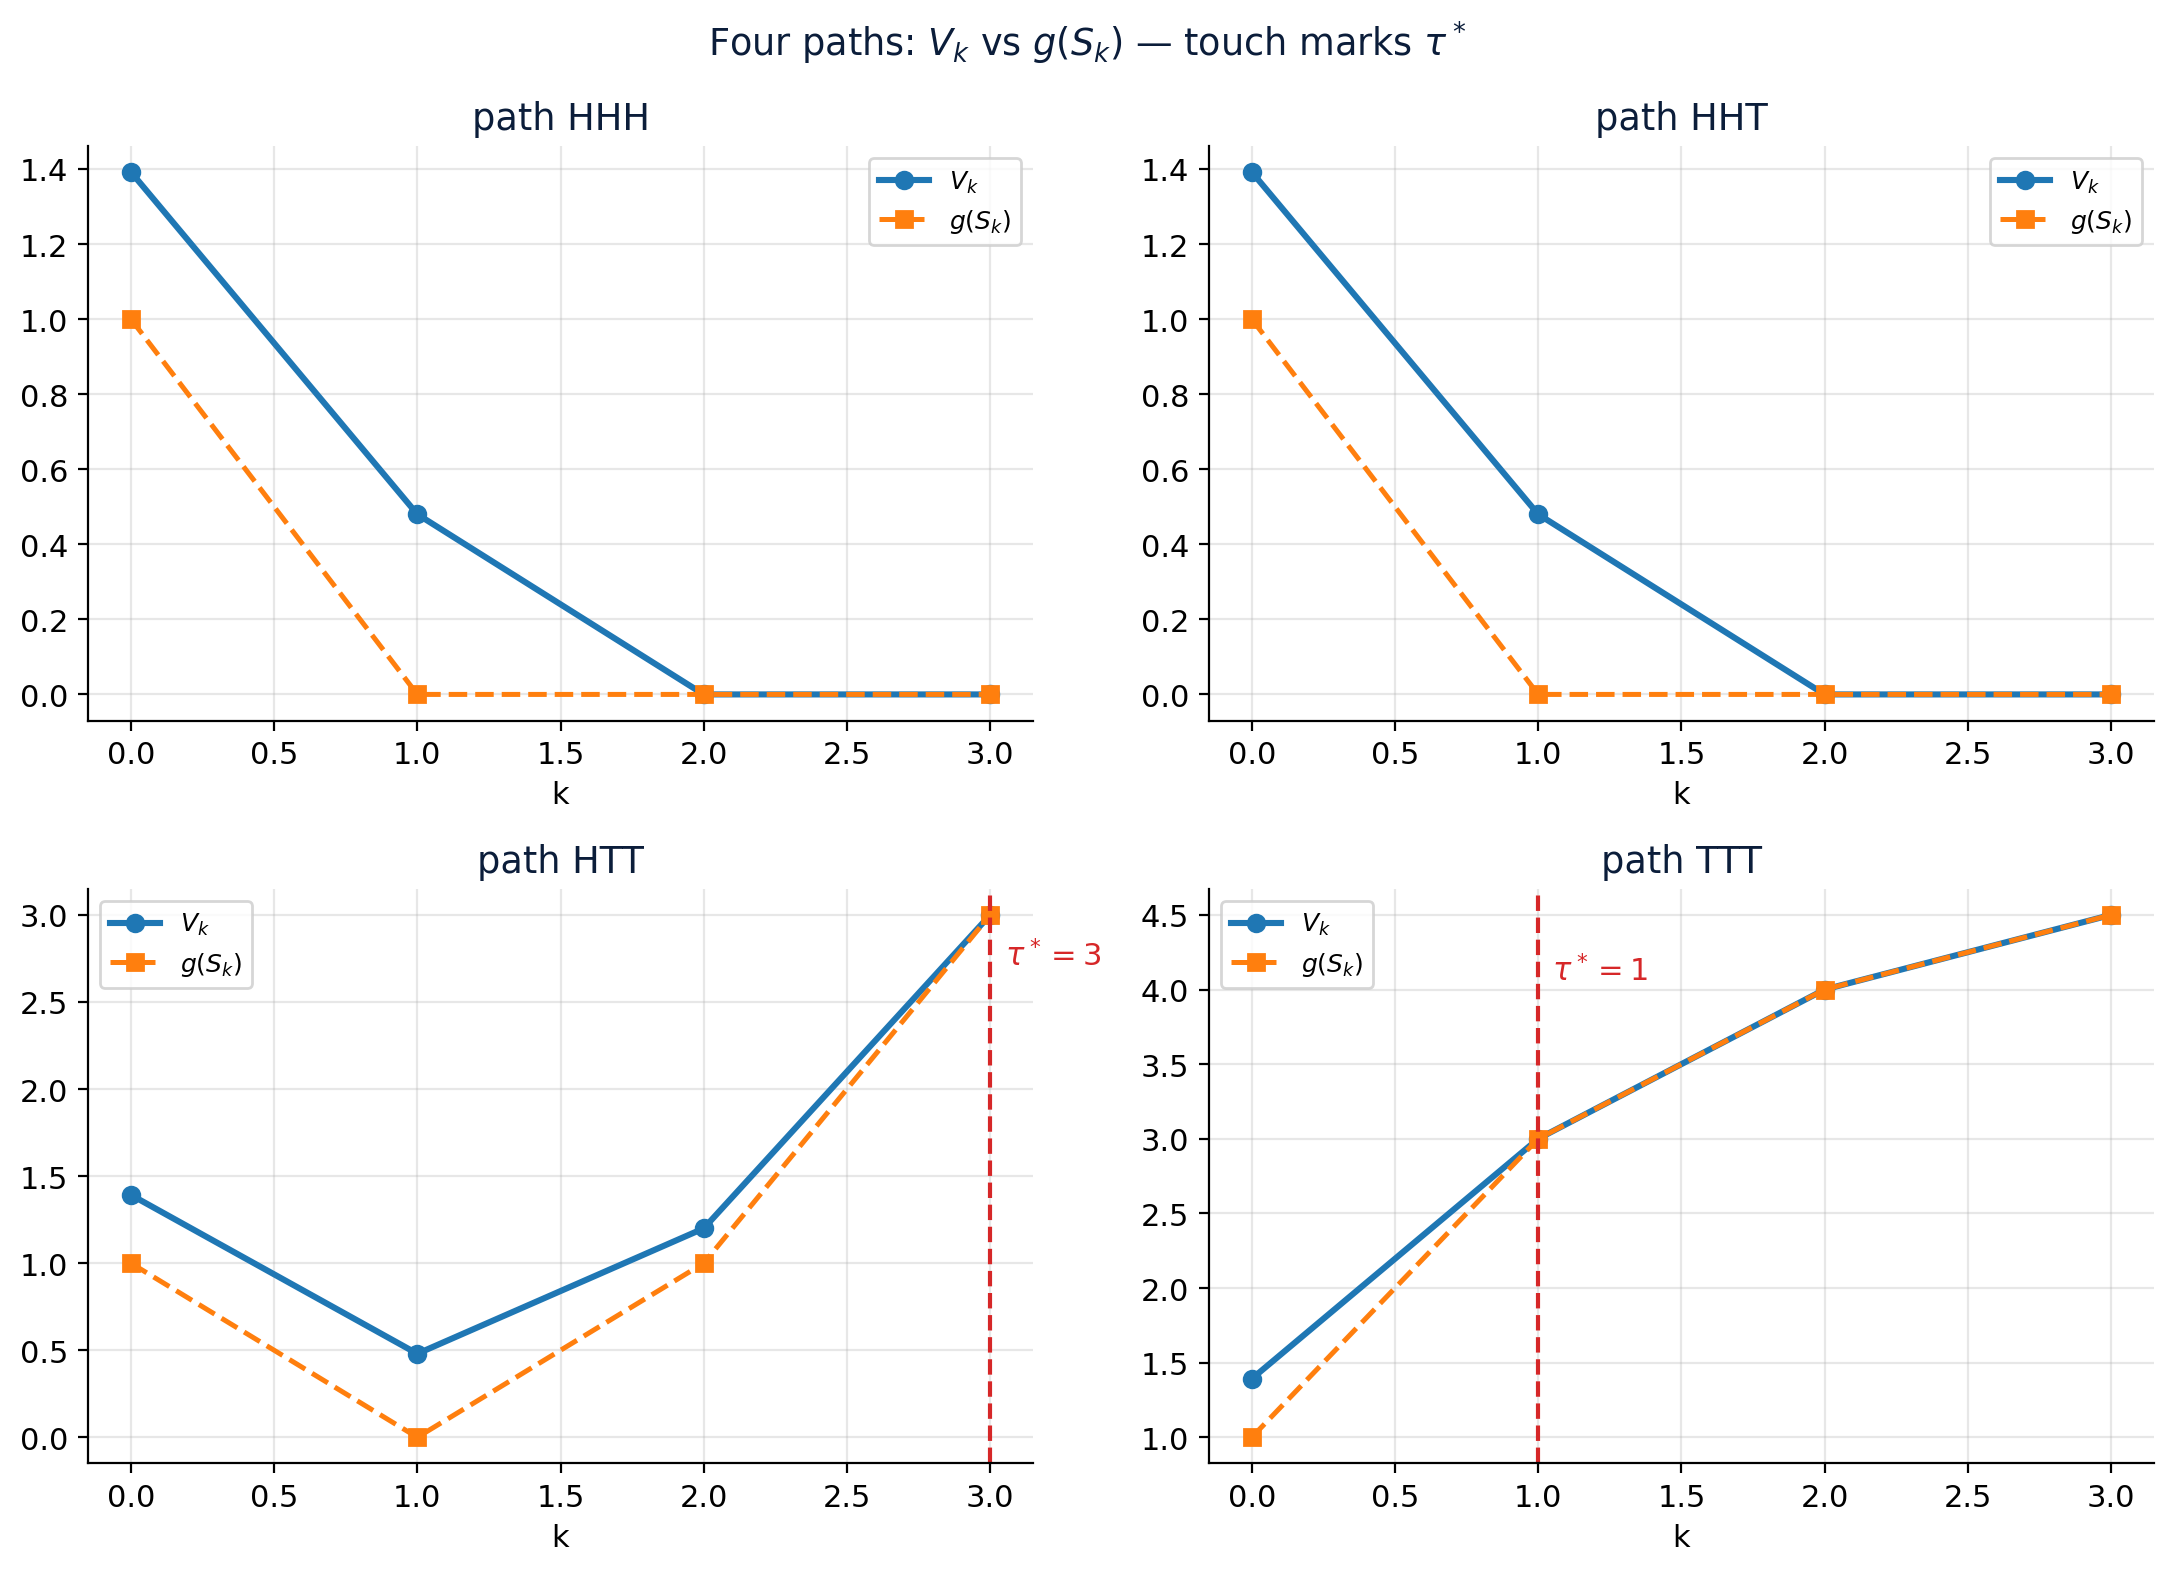
\includegraphics[keepaspectratio]{figures/ch04-tau-star-paths.png}}
\caption{Four paths of the ST put, each with \(V_k\) (blue) versus
\(g(S_k)\) (orange). The dashed red line marks \(\tau^*\) on each path
--- the first time blue and orange meet.}
\end{figure}

\begin{figure}
\centering
\pandocbounded{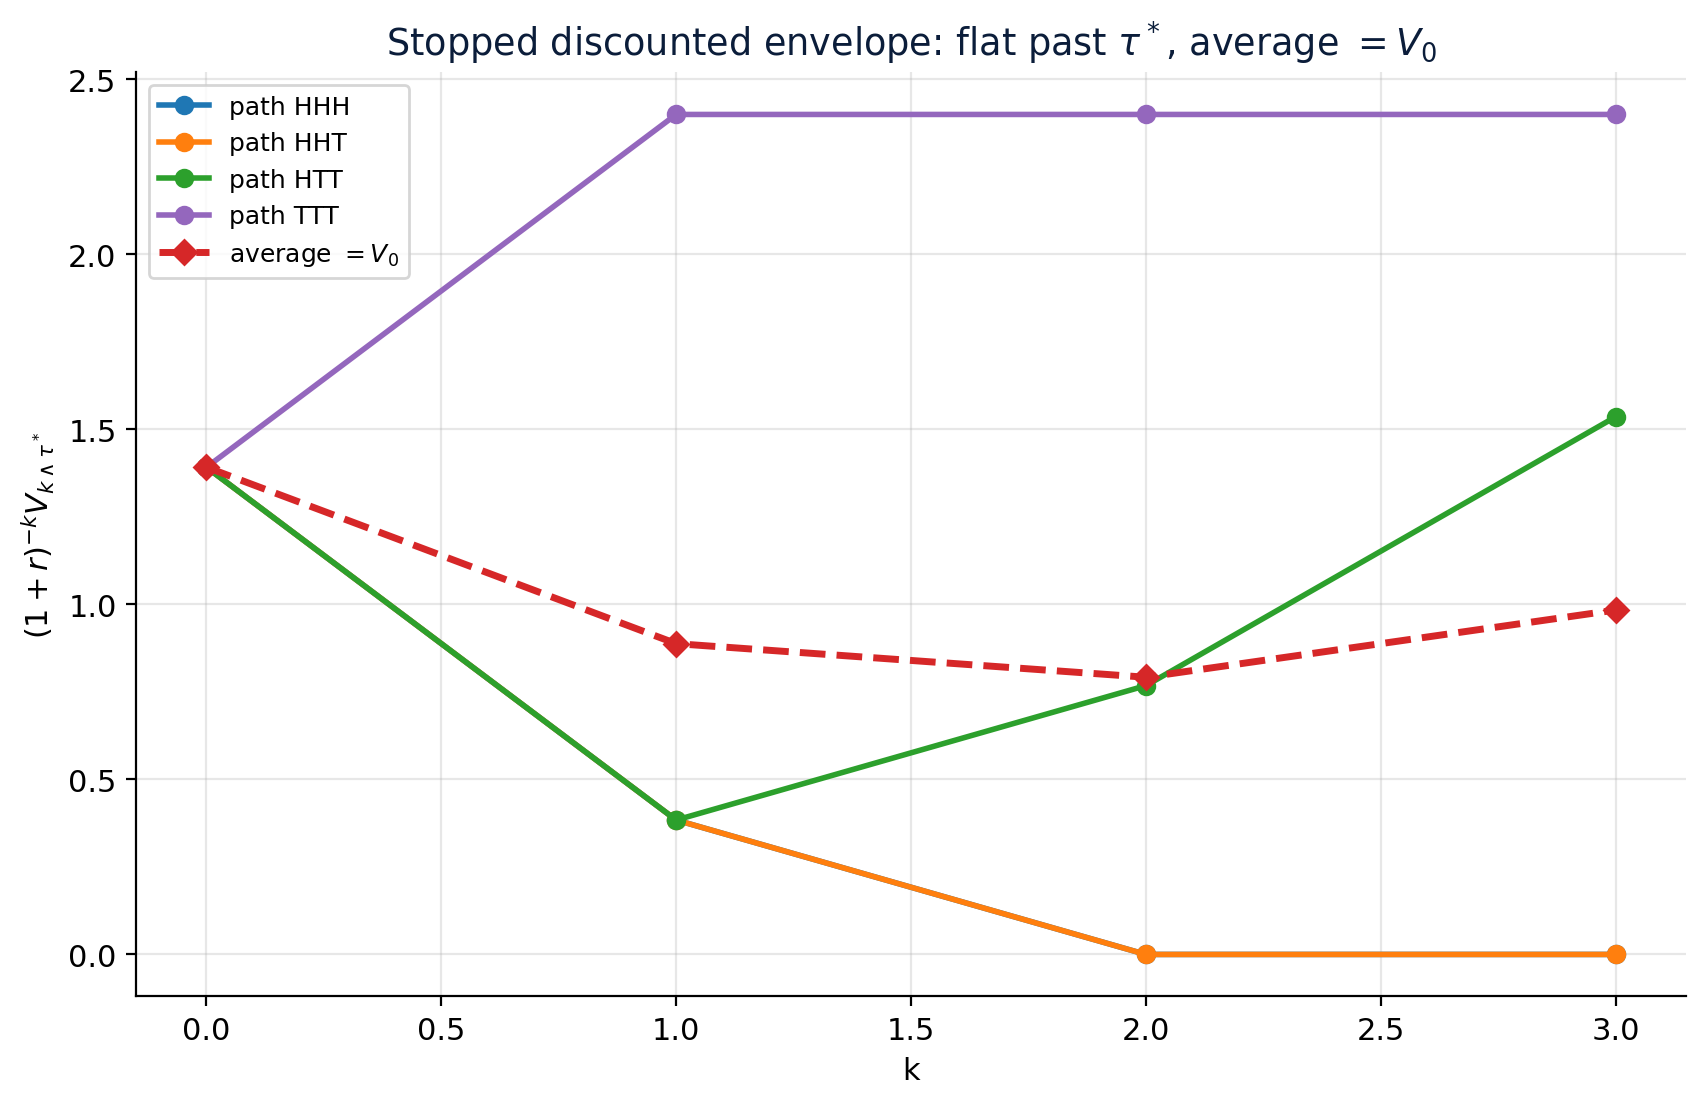
\includegraphics[keepaspectratio]{figures/ch04-stopped-mart.png}}
\caption{Stopped discounted Snell envelope, four paths. Each path's
curve is flat past its own \(\tau^*\) (the stopped process is constant).
The average across paths equals \(V_0\) --- and the conditional expected
drift is zero (martingale).}
\end{figure}

\subsection{4.4.5 Tables}\label{tables-7}

\textbf{Table 4.5.} ST put \(K=5\), path-by-path verification of
\(V_0 = \tilde{\mathbb{E}}[\beta^{\tau^*} g(S_{\tau^*})] = 1.36\).

(Reproduced from §4.4.2.)

\textbf{Table 4.6.} Realistic put \(K=100, n=3\), path-by-path
verification of \(V_0 = 4.907\).

(Reproduced from §4.4.3.)

\begin{center}\rule{0.5\linewidth}{0.5pt}\end{center}

\section{§4.5 Continuation region vs exercise
region}\label{continuation-region-vs-exercise-region}

\textbf{Punchline.} Colour every non-terminal node \textbf{red} if
\(V_k = g(S_k) > 0\) (exercise optimal) and \textbf{green} if
\(V_k > g(S_k)\) (continuation strictly better). For a put on a
non-dividend stock, the \textbf{exercise region is downward-closed in
\(S\)}: if you'd exercise at \((k, S)\), you'd also exercise at
\((k, S')\) for any \(S' < S\). The boundary between green and red is
the \textbf{exercise frontier} \(S^*(k)\).

\textbf{Intuition.} Exercising a put delivers \(K - S\). The smaller
\(S\), the bigger the lock-in and the less you'd want to wait (interest
on \(K\) has more impact). So once you're willing to exercise at \(S\),
you're a fortiori willing to exercise at anything lower. The exercise
frontier at each step is a \emph{moving threshold}: \(S^*(k)\). Below it
you exercise; above it you wait.

\subsection{4.5.1 Definitions}\label{definitions-14}

For a put with strike \(K\) on a non-dividend stock:

\[\text{Exercise region at } k : \quad E_k := \{S : V_k(S) = g(S) = K - S\} = \{S : S \le S^*(k)\},\]

\[\text{Continuation region at } k : \quad C_k := \{S : V_k(S) > g(S)\} = \{S : S > S^*(k)\}.\]

The frontier \(S^*(k)\) is \textbf{non-decreasing} in \(k\) for a
finite-horizon put (it grows toward maturity as the option premium
shrinks). It is \textbf{non-decreasing} in \(r\) (higher rates make
waiting more expensive). It is \textbf{non-increasing} in \(\sigma\)
(more volatility makes waiting more valuable).

\subsection{4.5.2 Worked examples}\label{worked-examples-1}

\textbf{Example 4.5.1 (ST put \(K=5\) frontier).} From the full Snell
table (§4.3.2):

{\def\LTcaptype{none} % do not increment counter
\begin{table}[H]
\centering
\begin{tabular}{|c|l|r|r|}
\toprule
\(k\) & exercise nodes & exercise \(S\) values & \(S^*(k)\) \\
\midrule



\(0\) & none & & \(-\infty\) \\
\(1\) & \((1,0)\) & \(\{2\}\) & \(2\) \\
\(2\) & \((2,0), (2,1)\) & \(\{1, 4\}\) & \(4\) \\
\bottomrule
\end{tabular}
\end{table}
}

\emph{Blank: exercise set is empty. \(-\infty\) = no \(S\) low enough to
trigger exercise.}

So the frontier on the toy lattice is \$S\^{}*(0) = \$ ``below all
reachable \(S\)'' (no exercise), \(S^*(1) = 2\), \(S^*(2) = 4\).
Monotone increasing.

\textbf{Example 4.5.2 (ST put \(K=4\) frontier).} With \(K = 4\) (less
ITM at start):

{\def\LTcaptype{none} % do not increment counter
\begin{table}[H]
\centering
\begin{tabular}{|c|l|r|}
\toprule
\(k\) & exercise nodes & \(S^*(k)\) \\
\midrule



\(0\) & none & \\
\(1\) & \((1,0)\) (\(S=2\)) & \(2\) \\
\(2\) & \((2,0)\) (\(S=1\)) & \(1\) \\
\bottomrule
\end{tabular}
\end{table}
}

\emph{Blank: no exercise frontier (set empty).}

Smaller exercise region --- at \(K = 4\), fewer nodes are deep enough to
be worth exercising.

\textbf{Example 4.5.3 (realistic put \(K=100\) frontier, \(n=3\)).} From
§4.3.3:

{\def\LTcaptype{none} % do not increment counter
\begin{table}[H]
\centering
\begin{tabular}{|c|r|r|}
\toprule
\(k\) & exercise \(S\) values & \(S^*(k)\) \\
\midrule



\(0\) & & \\
\(1\) & \(\{90\}\) & \(90.0\) \\
\(2\) & \(\{81\}\) & \(81.0\) \\
\(3\) & \(\{72.9, 89.1\}\) & \(89.1\) \\
\bottomrule
\end{tabular}
\end{table}
}

\emph{Blank: exercise set empty (no exercise at \(k=0\)).}

(Note that the terminal layer trivially has \(V_n = g_n\) wherever
\(g_n > 0\), so the ``frontier'' at \(n\) is the intrinsic boundary
\(K\) for put = \(100\). But the \emph{effective} frontier visible in
the tree is at the highest exercise-\(S\) node, \(89.1\).)

\textbf{Example 4.5.4 (longer maturity, \(n=4\)).} With
\(S_0 = 100, u=1.10, d=0.90, r=0.02, n=4\):

{\def\LTcaptype{none} % do not increment counter
\begin{table}[H]
\centering
\begin{tabular}{|c|l|r|}
\toprule
\(k\) & exercise nodes & \(S^*(k)\) \\
\midrule



\(0\) & none & \\
\(1\) & \(S_1 = 90\) & \(90.00\) \\
\(2\) & \(S_2 = 81\) & \(81.00\) \\
\(3\) & \(S_3 \in \{72.9, 89.1\}\) & \(89.10\) \\
\(4\) & \(\{65.61, 80.19, 98.01\}\) (terminal) & \(98.01\) \\
\bottomrule
\end{tabular}
\end{table}
}

\emph{Blank: exercise set empty at \(k=0\).}

The frontier creeps higher as we approach maturity --- the buyer becomes
less patient because there's less time for value to recover.

\textbf{Example 4.5.5 (frontier shifts with \(r\)).} At \(r = 0\): under
\(\tilde p = (1 + 0 - 0.9)/0.2 = 0.5\), the realistic put has \emph{no}
nodes with intrinsic exceeding continuation (you can verify by
recomputation). So \(S^*(k) = -\infty\) for all \(k < n\) --- never
exercise early. The American value equals the European, in line with
§4.7 below.

At \(r = 0.10\): under \(\tilde p = (1 + 0.1 - 0.9)/0.2 = 1\), the
lattice is degenerate (\(\tilde p = 1\)). Use \(r = 0.05\) instead:
\(\tilde p = 0.75\). Frontier moves up; more aggressive early exercise.

We'll see this graphically in the comparison figure.

\begin{figure}
\centering
\pandocbounded{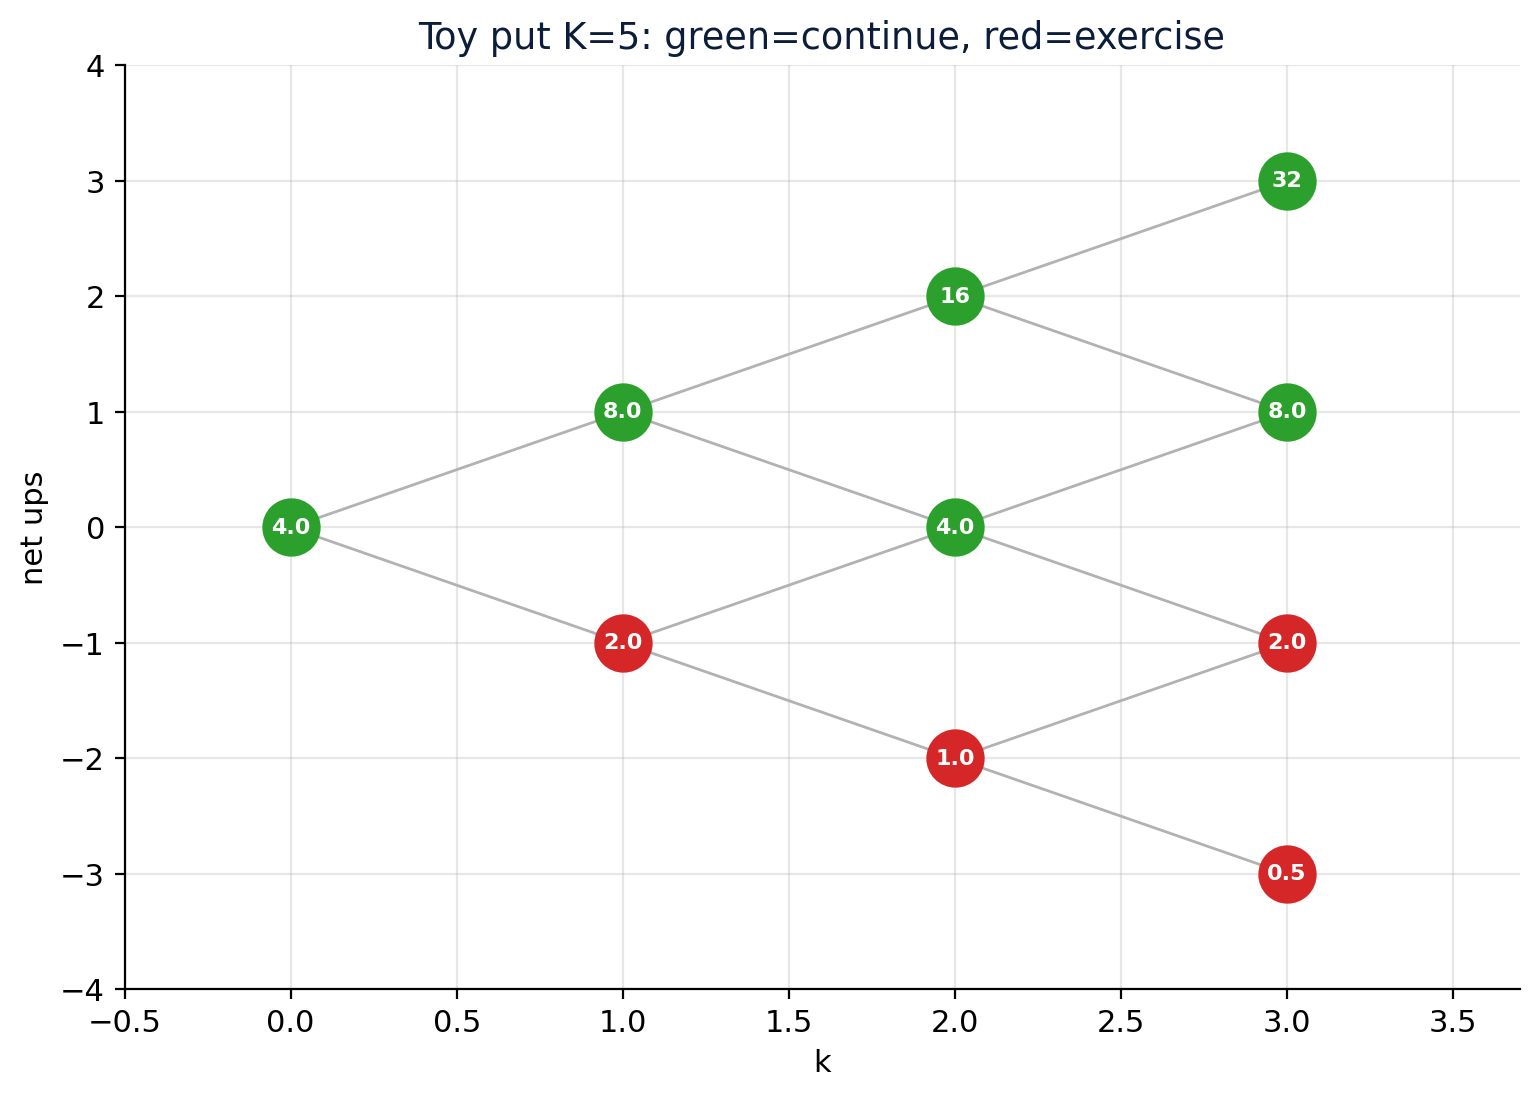
\includegraphics[keepaspectratio]{figures/ch04-frontier-st.png}}
\caption{ST put \(K=5\) frontier: continuation (green) vs exercise (red)
at every node.}
\end{figure}

\begin{figure}
\centering
\pandocbounded{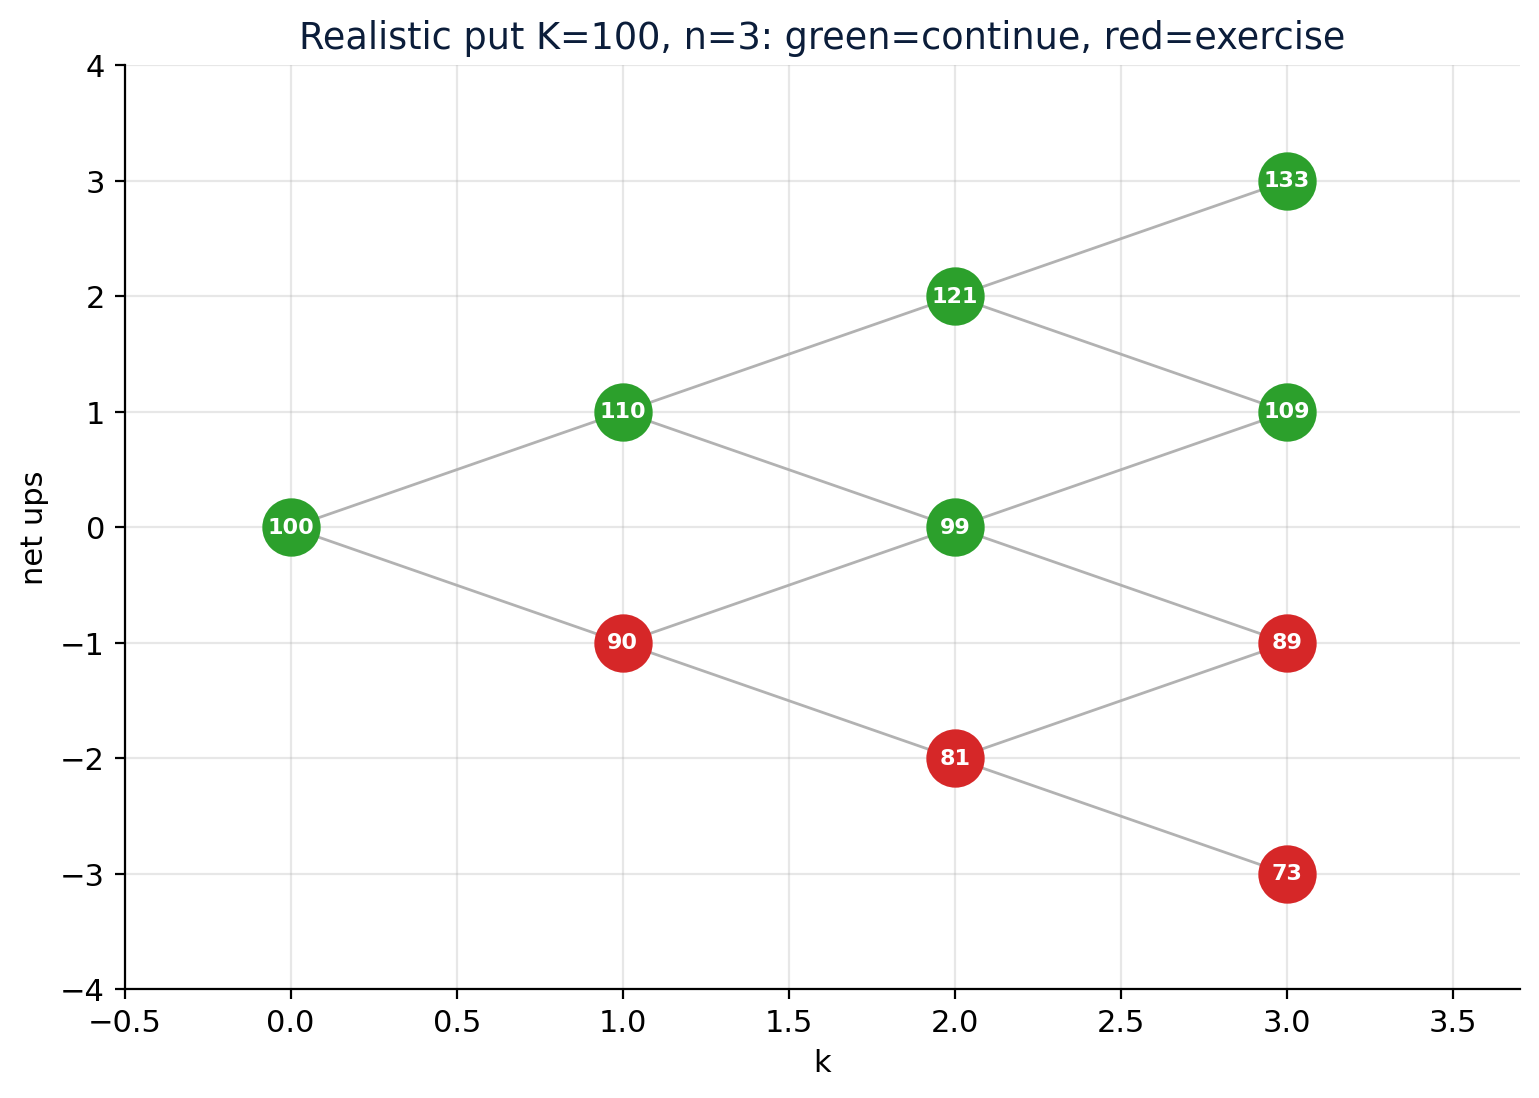
\includegraphics[keepaspectratio]{figures/ch04-frontier-rl.png}}
\caption{Realistic put \(K=100, n=3\) coloured tree.}
\end{figure}

\begin{figure}
\centering
\pandocbounded{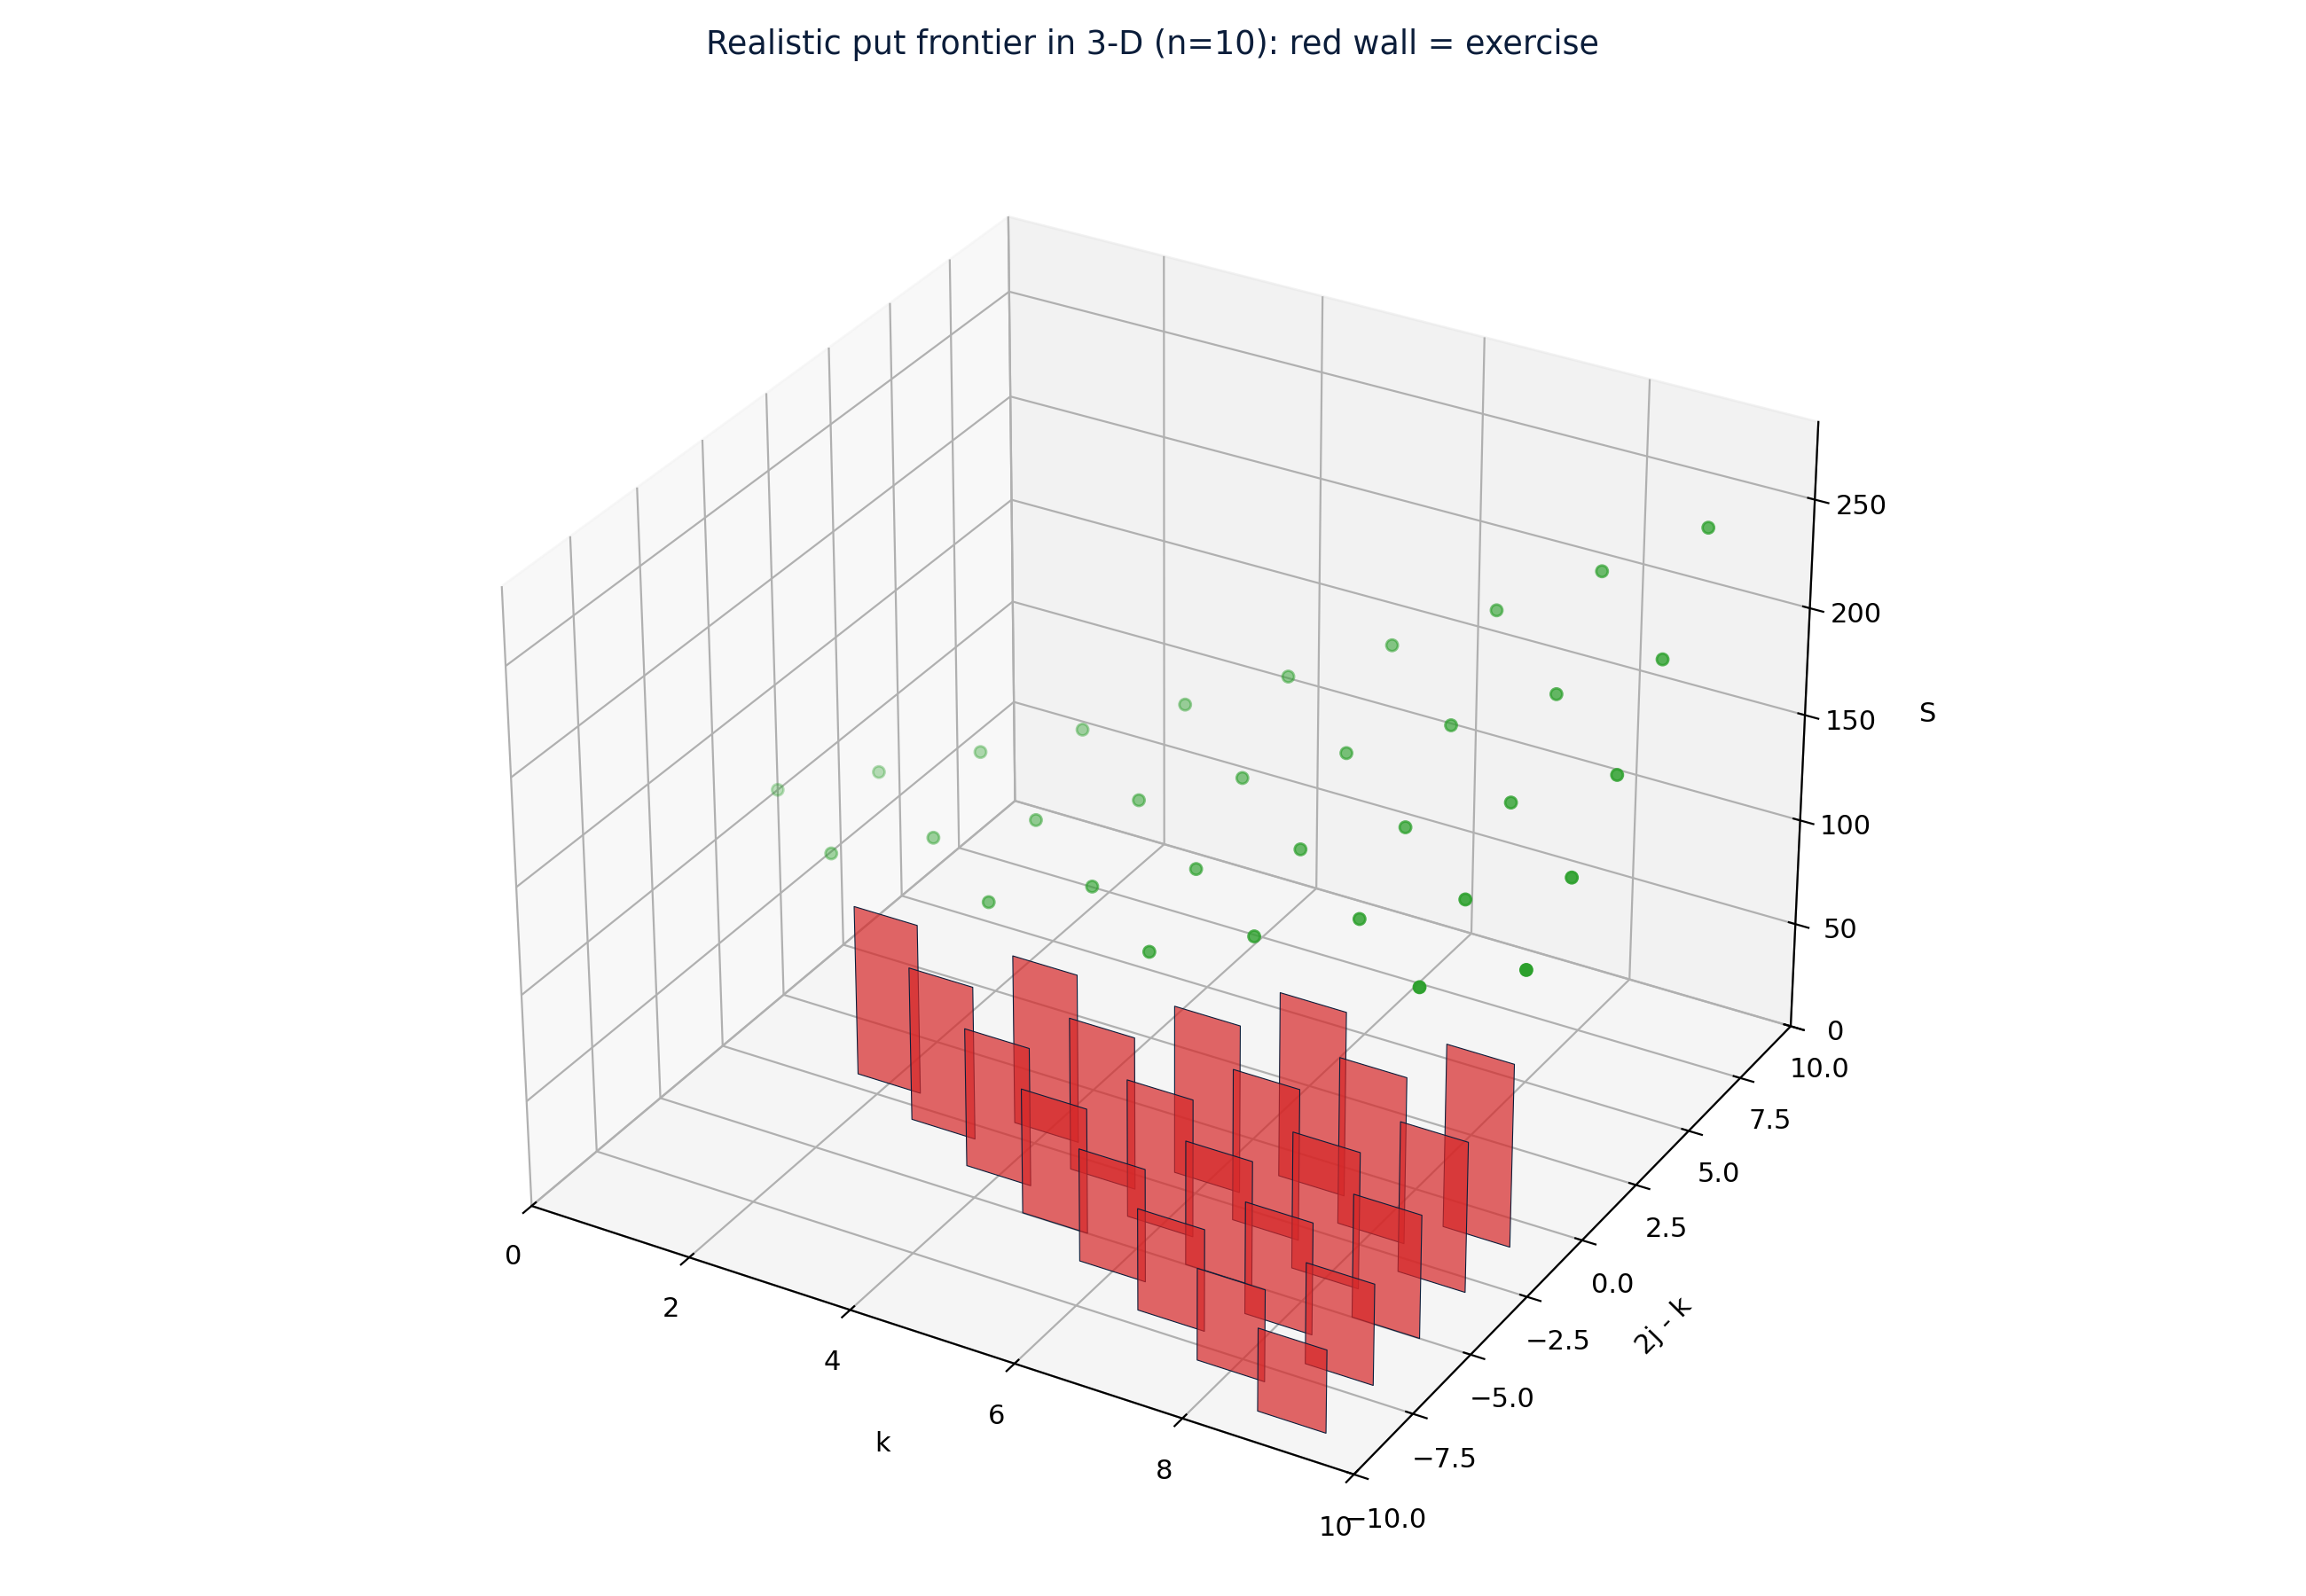
\includegraphics[keepaspectratio]{figures/ch04-frontier-3d.png}}
\caption{Exercise frontier \(S^*(k)\) in 3-D for the realistic put with
\(n=10\): red wall is the exercise region, green dots show continuation
nodes. The ``fence'' rises with \(k\).}
\end{figure}

\begin{figure}
\centering
\pandocbounded{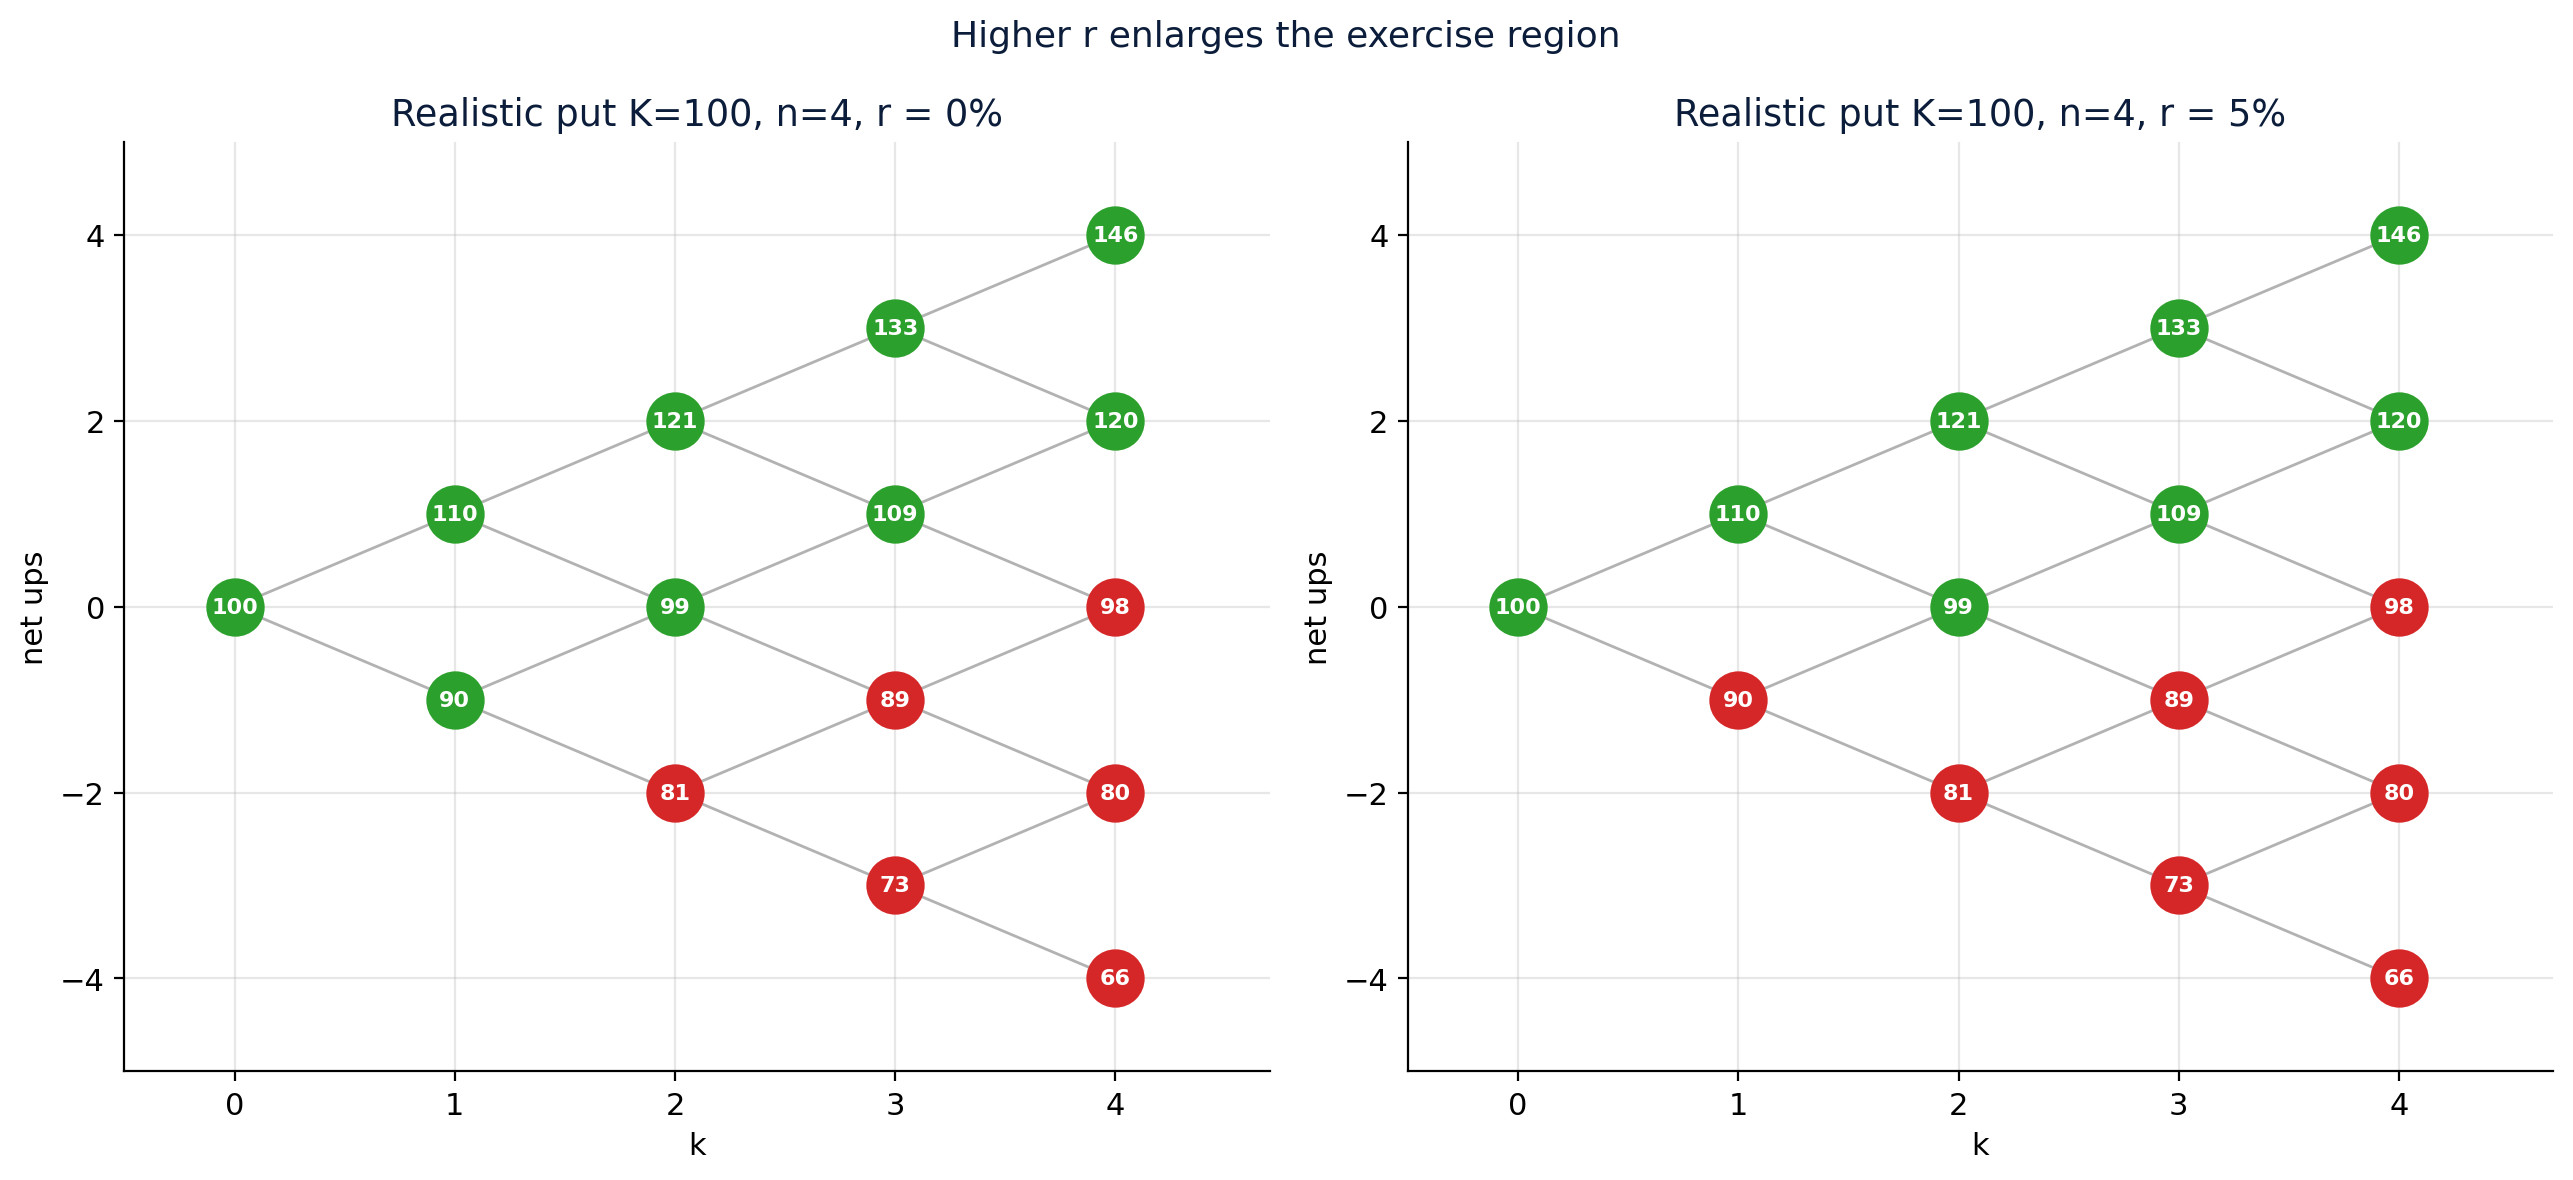
\includegraphics[keepaspectratio]{figures/ch04-frontier-r-compare.png}}
\caption{Same realistic put with \(r=0\%\) vs \(r=5\%\): higher \(r\)
enlarges the red exercise region. Interest forgone on the strike matters
more when rates are higher.}
\end{figure}

\subsection{4.5.3 Tables}\label{tables-8}

\textbf{Table 4.7.} Full Snell-envelope table for ST put \(K = 5\) with
regime.

{\def\LTcaptype{none} % do not increment counter
\begin{table}[H]
\centering
\begin{tabular}{|c|r|r|r|c|}
\toprule
\((k, \omega)\) & \(S\) & \(g\) & \(V\) & regime \\
\midrule



\((0, \cdot)\) & \(\phantom{0}4\) & \(1\) & \(1.36\) & C \\
\((1, H)\) & \(\phantom{0}8\) & \(0\) & \(0.40\) & C \\
\((1, T)\) & \(\phantom{0}2\) & \(3\) & \(3.00\) & \textbf{E} \\
\((2, HH)\) & \(16\) & \(0\) & \(0.00\) & term \\
\((2, HT/TH)\) & \(\phantom{0}4\) & \(1\) & \(1.00\) & term-E \\
\((2, TT)\) & \(\phantom{0}1\) & \(4\) & \(4.00\) & term-E \\
\bottomrule
\end{tabular}
\end{table}
}

\emph{Legend.} C = continue. E = exercise. term = terminal OTM. term-E =
terminal in-the-money.*

\textbf{Table 4.8.} \(S^*(k)\) for a 10-step realistic put \(K=100\),
\(r=2\%\):

{\def\LTcaptype{none} % do not increment counter
\begin{table}[H]
\centering
\begin{tabular}{|c|r|}
\toprule
\(k\) & \(S^*(k)\) \\
\midrule



\(\phantom{0}0\) & \\
\(\phantom{0}1\) & \\
\(\phantom{0}2\) & \\
\(\phantom{0}3\) & \(\phantom{0}81.0\) \\
\(\phantom{0}4\) & \(\phantom{0}81.0\) \\
\(\phantom{0}5\) & \(\phantom{0}89.1\) \\
\(\phantom{0}6\) & \(\phantom{0}89.1\) \\
\(\phantom{0}7\) & \(\phantom{0}89.1\) \\
\(\phantom{0}8\) & \(\phantom{0}89.1\) \\
\(\phantom{0}9\) & \(\phantom{0}89.1\) \\
\(10\) & \(100.0\) (terminal) \\
\bottomrule
\end{tabular}
\end{table}
}

\emph{Blank: no exercise nodes at that \(k\) (frontier empty).}

(Numerical values produced by the figure-builder.)

\begin{center}\rule{0.5\linewidth}{0.5pt}\end{center}

\section{§4.6 American call = European call (no
dividends)}\label{american-call-european-call-no-dividends}

\textbf{Punchline.} For a non-dividend-paying stock, the American call
equals the European call. Early exercise is \emph{never} optimal. The
discounted call payoff \(\beta^k(S_k - K)^+\) is a
\(\tilde{\mathbb{P}}\)-submartingale, so its conditional expectation
grows --- waiting always dominates.

\textbf{Intuition.} Exercising a call delivers \(S - K\) immediately.
Waiting one period gives you the option to delay receiving \(K\) (worth
\(K - \beta K\) in interest savings) and still capture any upside (you
can always exercise next period instead). With no dividends
interrupting, you have nothing to give up by waiting --- and a positive
interest carry to gain.

\subsection{4.6.1 The proof (no calculus)}\label{the-proof-no-calculus}

We show \(\beta^k (S_k - K)^+\) is a
\(\tilde{\mathbb{P}}\)-submartingale, then conclude that the European
recursion already dominates the intrinsic.

\textbf{Step 1.} \(\beta^k S_k\) is a \(\tilde{\mathbb{P}}\)-martingale
(Ch 3, §3.5), so
\(\tilde{\mathbb{E}}[\beta^{k+1}S_{k+1}\mid\mathcal F_k] = \beta^k S_k\).

\textbf{Step 2.} Compute the one-step conditional expectation of the
discounted \emph{un-truncated} payoff \(\beta^k(S_k - K)\):

\[\tilde{\mathbb{E}}\!\left[\beta^{k+1}(S_{k+1} - K)\mid\mathcal F_k\right] = \tilde{\mathbb{E}}\!\left[\beta^{k+1} S_{k+1}\mid\mathcal F_k\right] - \beta^{k+1} K = \beta^k S_k - \beta^{k+1} K.\]

Using \(\beta < 1\):

\[\beta^k S_k - \beta^{k+1} K \;>\; \beta^k S_k - \beta^k K = \beta^k(S_k - K).\]

So
\(\tilde{\mathbb{E}}[\beta^{k+1}(S_{k+1} - K)\mid\mathcal F_k] > \beta^k(S_k - K)\)
--- the discounted \emph{un-truncated} payoff is a strict submartingale.

\textbf{Step 3.} Truncation at zero (the \((\cdot)^+\) part) preserves
submartingale property by Jensen's inequality applied to the convex
function \(x \mapsto x^+\). Equivalently,
\((S_{k+1} - K)^+ \ge (S_{k+1} - K)\) and \(\ge 0\), so

\[\begin{aligned}
\tilde{\mathbb{E}}\!\left[\beta^{k+1}(S_{k+1} - K)^+\mid\mathcal F_k\right] &\ge \tilde{\mathbb{E}}\!\left[\beta^{k+1}(S_{k+1} - K)\mid\mathcal F_k\right] \\
&= \beta^k S_k - \beta^{k+1} K \ge \beta^k(S_k - K),
\end{aligned}\]

and also \(\ge 0\), so it's \(\ge \beta^k(S_k - K)^+\). The discounted
call payoff \(\beta^k(S_k - K)^+\) is a
\(\tilde{\mathbb{P}}\)-submartingale.

\textbf{Step 4.} Apply Snell. The American call Snell envelope \(V_k\)
at every node satisfies

\[V_k = \max\{(S_k - K)^+,\, \beta\tilde{\mathbb{E}}[V_{k+1}\mid\mathcal F_k]\}.\]

Define
\(W_k := \beta^k\tilde{\mathbb{E}}[(S_n - K)^+\mid\mathcal F_k]/\beta^k = \tilde{\mathbb{E}}[\beta^{n-k}(S_n - K)^+\mid\mathcal F_k]\).
This is the European call value at \((k, S_k)\). By submartingality of
discounted intrinsic, \(W_k \ge (S_k - K)^+\) at every node. So in the
recursion the \(\max\) is always achieved by the continuation, never by
exercising. Hence \(V_k = W_k\) --- the European value, at every node.

\textbf{Conclusion.} \(V_0^{\text{Am call}} = V_0^{\text{Eu call}}\),
and exercising early at any node is strictly suboptimal.

\subsection{4.6.2 Worked examples}\label{worked-examples-2}

\textbf{Example 4.6.1 (ST call \(K=5\), all-green tree).} Toy lattice,
call payoffs.

Terminal payoffs with \(S_0 = 4, K = 5\):

\begin{itemize}
\item
  \(S_2 = 16 \to g = 11\)
\item
  \(S_2 = 4 \to g = 0\)
\item
  \(S_2 = 1 \to g = 0\)
\item
  \(V_1(H), S = 8\): intrinsic \(3\). Continuation:
  \(\beta\cdot \tfrac{1}{2}(11 + 0) = 0.8\cdot 5.5 = 4.40\).
  \(V_1(H) = \max\{3, 4.40\} = 4.40\) → \textbf{continue} ✓
\item
  \(V_1(T), S = 2\): intrinsic \(0\). Continuation:
  \(\beta\cdot\tfrac{1}{2}(0 + 0) = 0\). \(V_1(T) = 0\) → continue
  trivially.
\item
  \(V_0, S = 4\): intrinsic \(0\). Continuation:
  \(\beta\cdot\tfrac{1}{2}(4.40 + 0) = 1.76\). \(V_0 = 1.76\).
\end{itemize}

European: same recursion without the max --- same number, \(1.76\). ✓
--- American \(=\) European.

\textbf{Example 4.6.2 (realistic call \(K=100\), \(n=3\)).} Already
computed in §4.1.2: European = \(10.360\), and the recursion never picks
intrinsic over continuation, so American = \(10.360\).

\textbf{Example 4.6.3 (submartingale check, ST).} At \((1, 1)\) where
\(S = 8\), \(g = 3\):
\(\tilde{\mathbb{E}}[\beta\cdot g(S_2)\mid\mathcal F_1, H] = \beta\cdot\tfrac{1}{2}(11 + 0) = 4.40 > 3\).
Discounted-payoff submartingale property satisfied with strict
inequality at this node. ✓

\textbf{Example 4.6.4 (with dividend, early exercise can become
optimal).} Suppose the stock pays a proportional dividend yield \(q\)
per period: after each move the holder receives \(q\cdot S\) in cash and
the stock drops to \((1-q)\cdot S\). With cum-dividend factors \(u, d\),
the no-arbitrage condition is

\[\tilde p_q\cdot u\cdot (1-q) + (1-\tilde p_q)\cdot d\cdot (1-q) = 1 + r\]

(total return = stock change + dividend, discounted = 1), giving

\[\tilde p_q \;=\; \frac{(1+r)/(1-q) - d}{u - d}.\]

For the toy with \(q = 0.10\):
\(\tilde p_q = (1.25/0.9 - 0.5)/1.5 \approx 0.593\).

The qualitative story: holding the call one extra period earns interest
on the strike \(K\) saved (worth roughly \(rK\cdot\beta\) per period)
but \emph{forgoes} the dividend \(q\cdot S\) that the stock-holder
collects. When the dividend forgone exceeds the interest saved ---
roughly when \(q\cdot S > r\cdot K\), i.e., the stock is sufficiently
deep in the money --- early exercise wins. This crossover
\(S^* \approx rK/q\) is the upper exercise boundary, the call analogue
of the put frontier of §4.5 (with the inequality reversed: exercise the
call when \(S\) is \emph{above} the frontier). For the toy with
\(K = 3, q = 0.10\), the crossover sits near
\(S = rK/q = 0.25\cdot 3/0.10 = 7.5\), which is right between the two
reachable \(k=1\) stock values (\(8\) and \(2\)) --- so the up-node
\(S=8\) is the first node to trigger early exercise.

\textbf{Example 4.6.5 (continuous-dividend preview).} In Chapter 8 we'll
see the continuous-dividend limit: a stock paying continuous yield \(q\)
has Black--Scholes-style American call value strictly less than its
European counterpart whenever \(q > 0\), with early exercise optimal
once

\[S \ge S^*(t) \text{ for some moving boundary } S^*(t),\]

analogous to the put frontier of §4.5 but on the upper side. Discrete
approximation: the lattice with \(q\) per period converges to the
continuous-\(q\) Black--Scholes-Merton model.

\begin{figure}
\centering
\pandocbounded{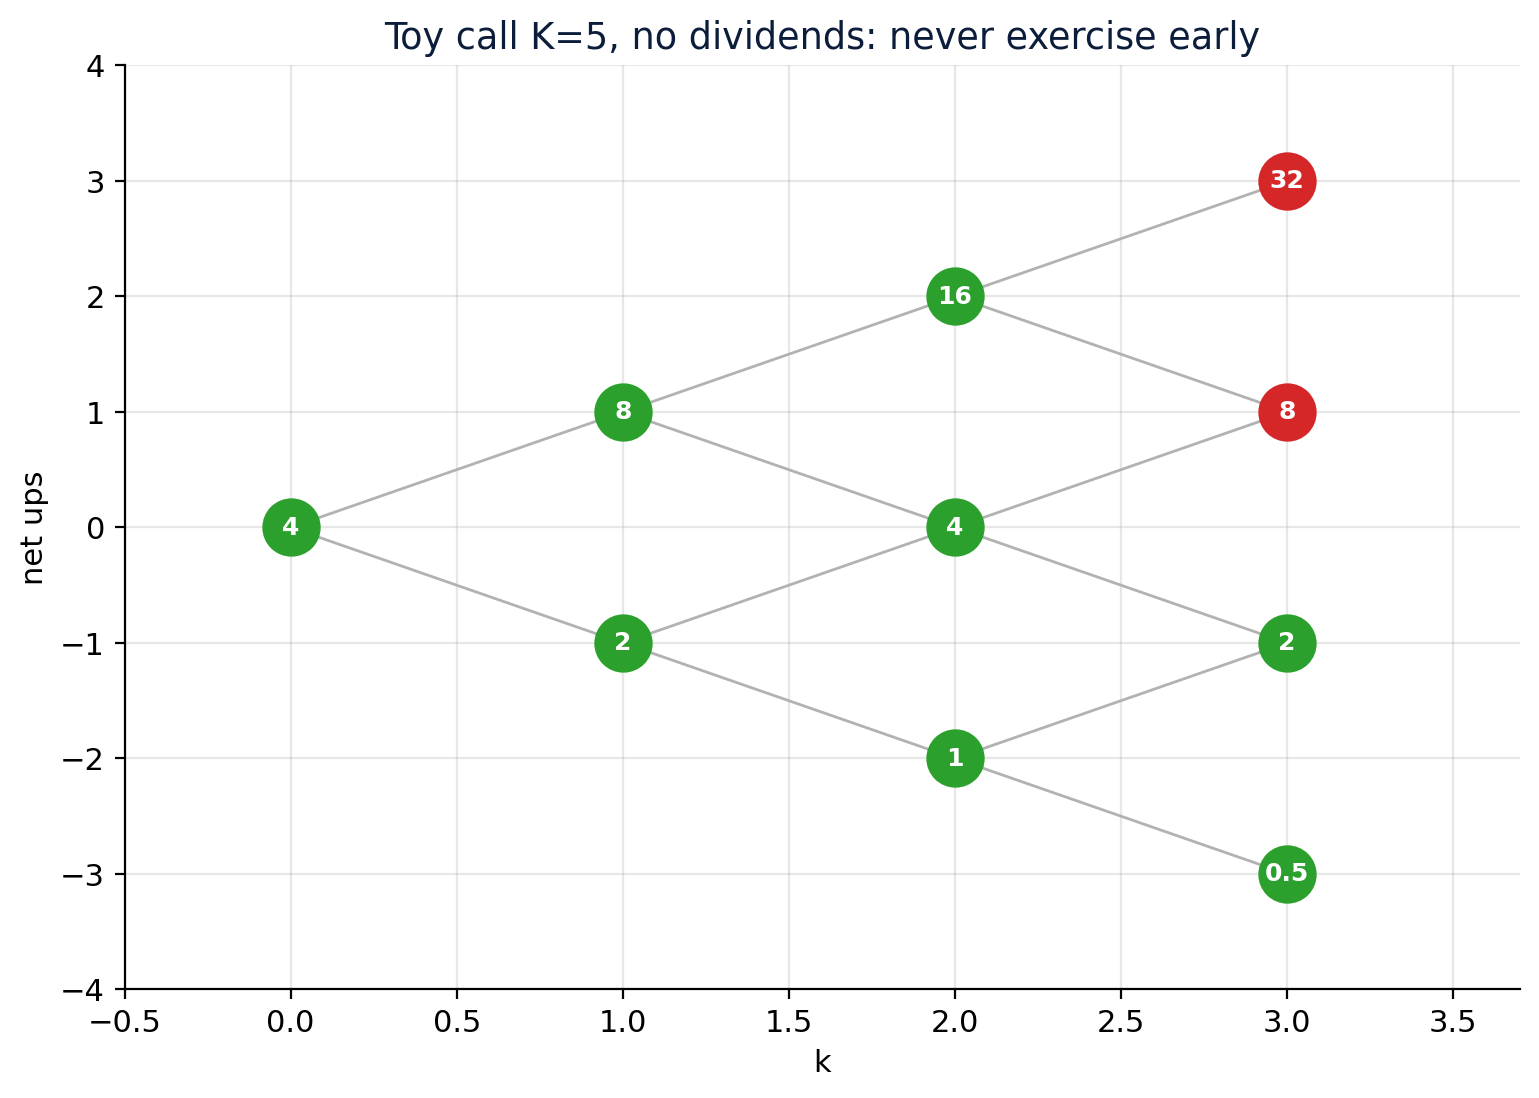
\includegraphics[keepaspectratio]{figures/ch04-call-tree-all-green.png}}
\caption{ST call \(K=5\), no dividends: all non-terminal nodes are green
--- never exercise.}
\end{figure}

\begin{figure}
\centering
\pandocbounded{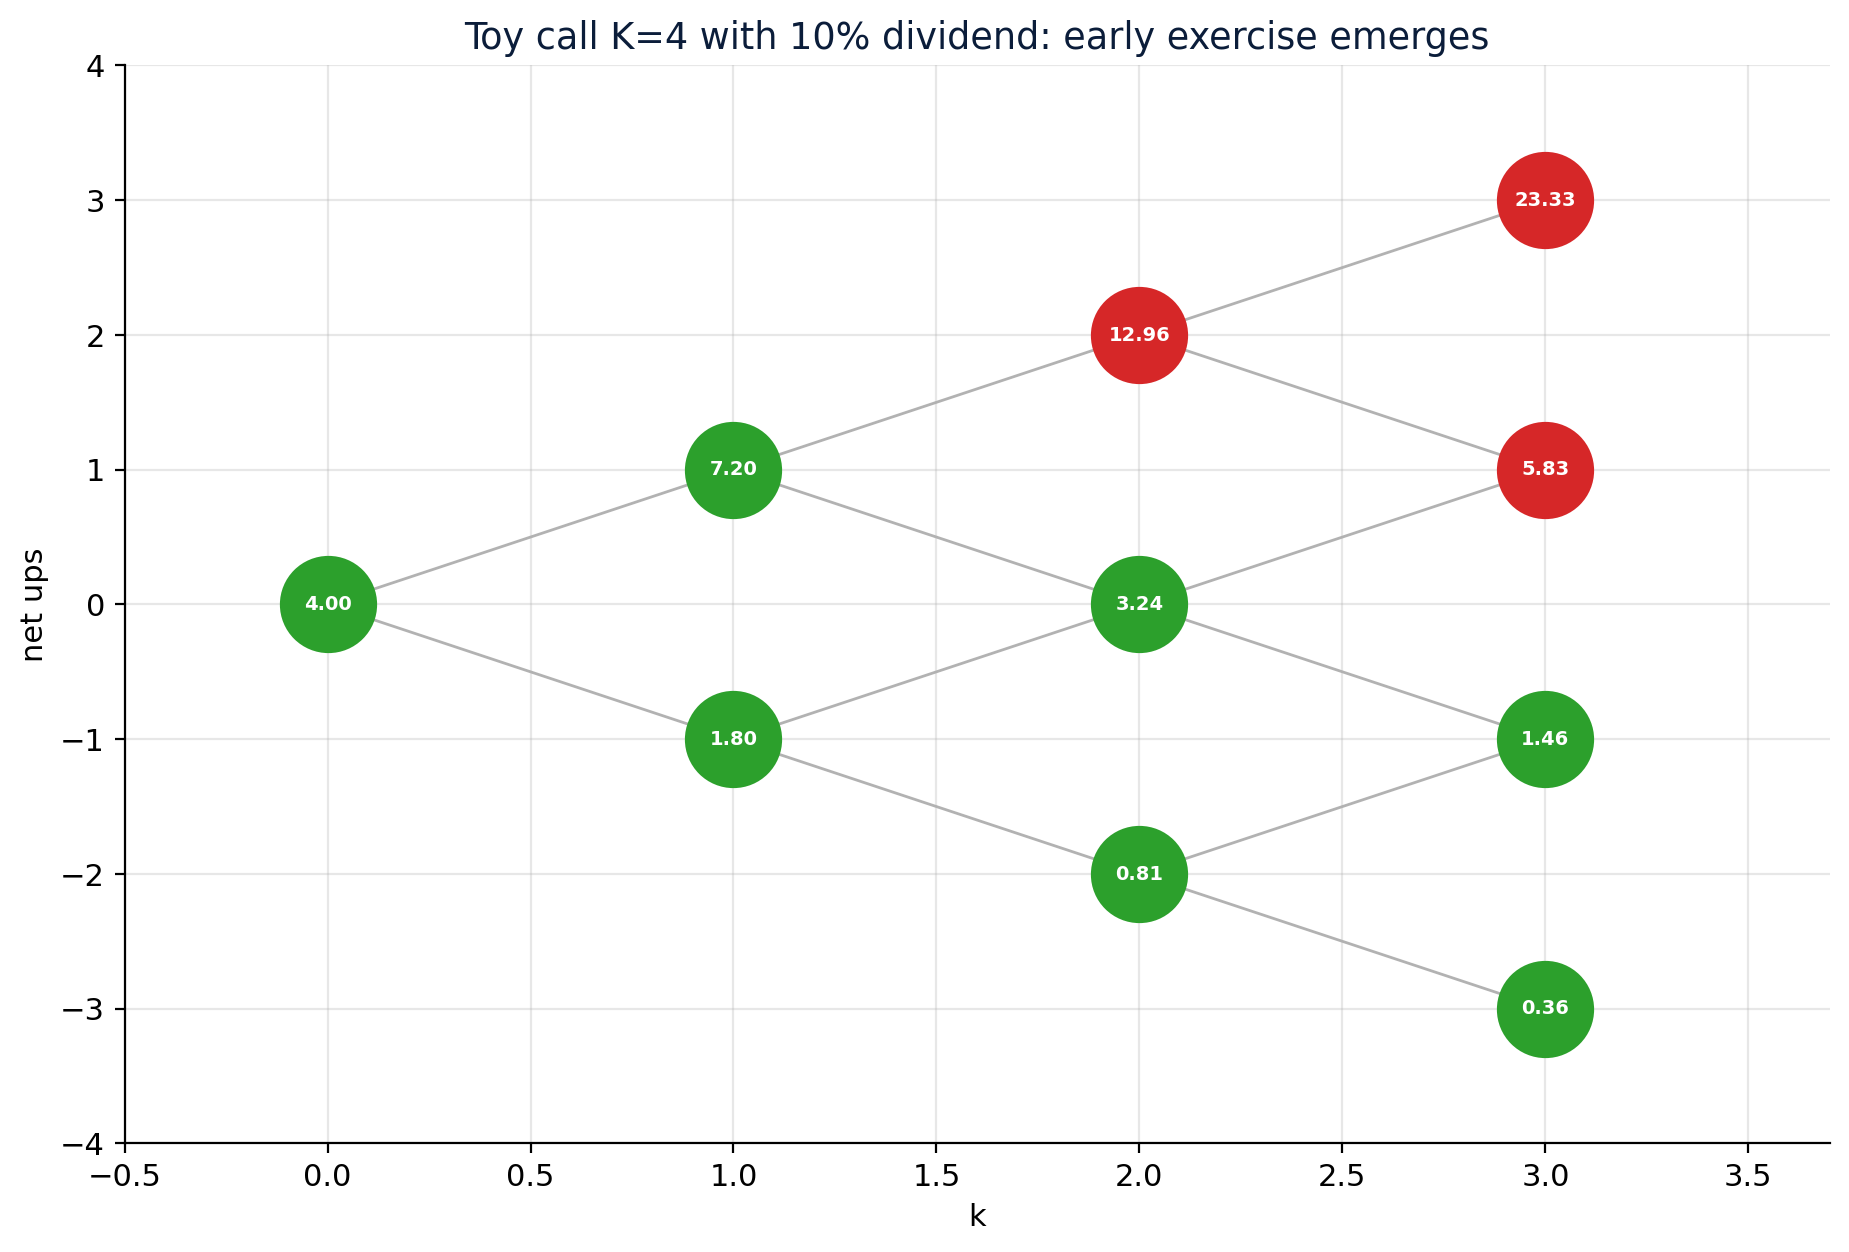
\includegraphics[keepaspectratio]{figures/ch04-call-tree-with-div.png}}
\caption{ST call \(K=4\) with 10\% per-period dividend: a few red nodes
appear --- early exercise can become optimal.}
\end{figure}

\begin{figure}
\centering
\pandocbounded{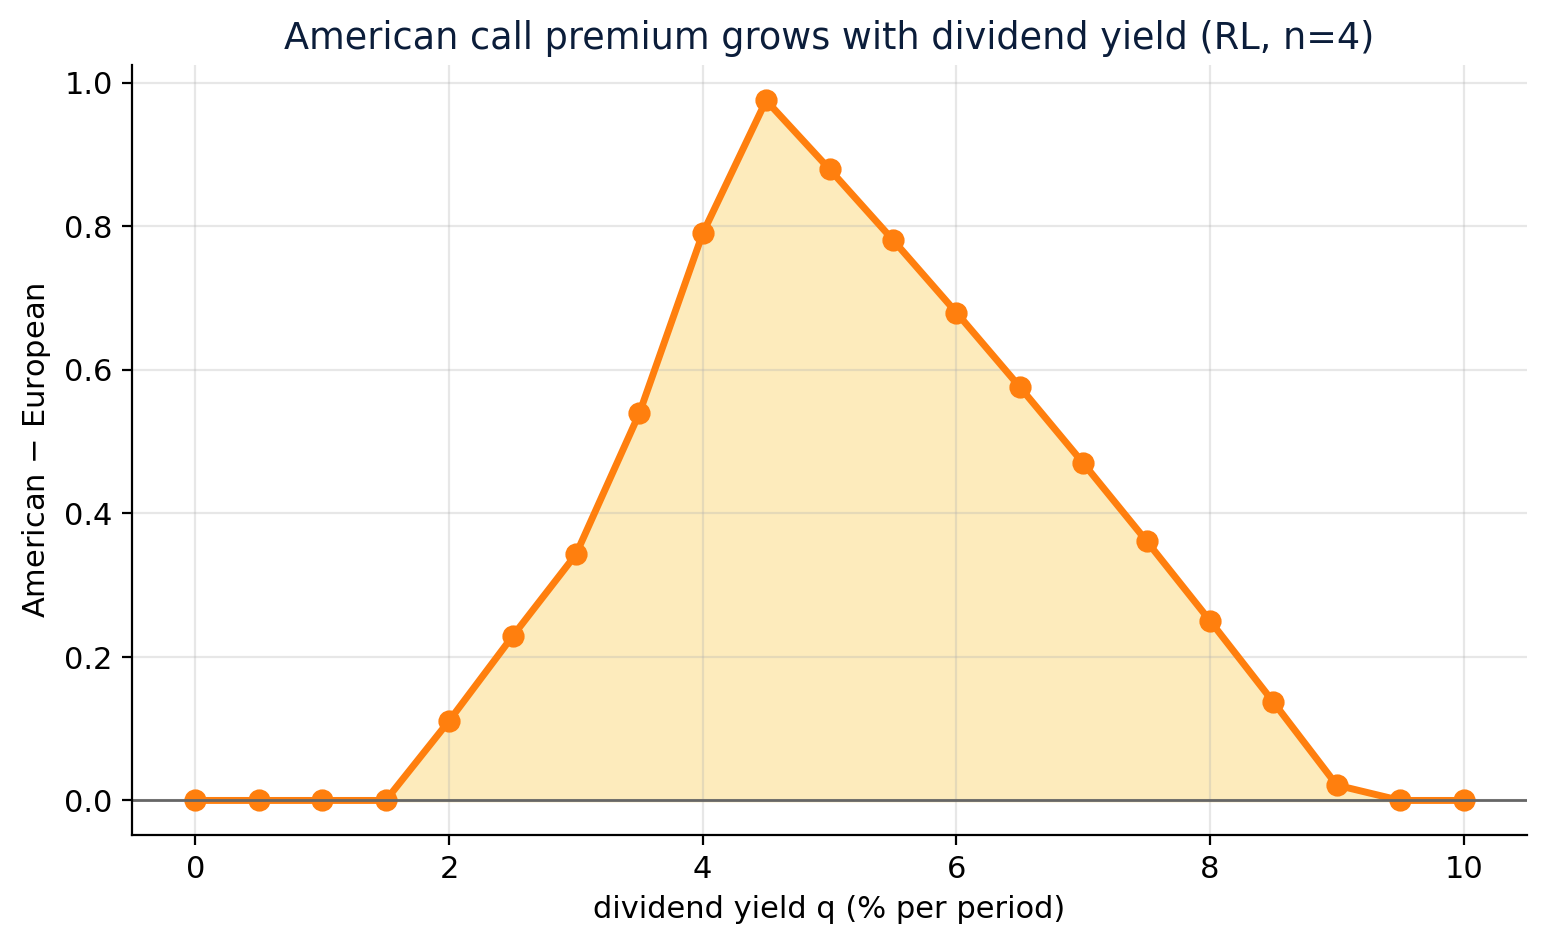
\includegraphics[keepaspectratio]{figures/ch04-am-eu-diff-vs-div.png}}
\caption{American minus European call value as a function of dividend
yield (RL lattice, \(n=4\)). Without dividends the gap is zero; with
dividends it grows.}
\end{figure}

\subsection{4.6.3 Tables}\label{tables-9}

\textbf{Table 4.9.} American vs European call on the toy lattice across
strikes (no dividends). The gap is zero at every strike --- early
exercise is never optimal on a non-dividend stock.

{\def\LTcaptype{none} % do not increment counter
\begin{table}[H]
\centering
\begin{tabular}{|c|r|r|r|}
\toprule
\(K\) & \(V_0^{\text{Am call}}\) & \(V_0^{\text{Eu call}}\) & gap \\
\midrule



\(2\) & \(2.88\) & \(2.88\) & \(0.00\) \\
\(3\) & \(2.40\) & \(2.40\) & \(0.00\) \\
\(4\) & \(1.92\) & \(1.92\) & \(0.00\) \\
\(5\) & \(1.76\) & \(1.76\) & \(0.00\) \\
\(6\) & \(1.60\) & \(1.60\) & \(0.00\) \\
\bottomrule
\end{tabular}
\end{table}
}

\textbf{Table 4.10.} Same realistic call \(K = 100, n = 4\) with
per-period dividend yield \(q\):

{\def\LTcaptype{none} % do not increment counter
\begin{table}[H]
\centering
\begin{tabular}{|c|r|r|r|}
\toprule
\(q\) & \(V_0^{\text{Am call}}\) & \(V_0^{\text{Eu call}}\) & gap \\
\midrule



\(0.00\) & \(12.66\) & \(12.66\) & \(\phantom{+}0.00\) \\
\(0.02\) & \(11.59\) & \(11.45\) & \(+0.14\) \\
\(0.04\) & \(10.61\) & \(10.29\) & \(+0.32\) \\
\(0.06\) & \(\phantom{0}9.74\) & \(\phantom{0}9.21\) & \(+0.53\) \\
\(0.10\) & \(\phantom{0}8.20\) & \(\phantom{0}7.20\) & \(+1.00\) \\
\bottomrule
\end{tabular}
\end{table}
}

(Numerical values produced by the figure-builder; exact figures depend
on the lattice details.)

\begin{center}\rule{0.5\linewidth}{0.5pt}\end{center}

\section{§4.7 American put --- when early exercise
pays}\label{american-put-when-early-exercise-pays}

\textbf{Punchline.} A put pays \(K - S\). Deep ITM, this lock-in is
sitting in cash earning no interest, and the upside (if \(S\) rebounds)
was capped at \(K\) anyway. Early exercise frees the cash to earn \(r\).
The exercise region \textbf{grows with \(r\)} and \textbf{shrinks with
\(\sigma\)}. Time to maturity also matters: shorter horizon → less
option premium → larger exercise region.

\textbf{Intuition (the calculus-free version).} The put-holder is short
the stock and long a cash account at strike \(K\) --- that's what
intrinsic delivers. By holding the put instead of exercising, you delay
receiving the \(K\) --- you are effectively \emph{lending} the seller
the strike for an extra period. If the rate is high, that delay is
expensive. The decision to exercise early is a trade-off: interest gain
(always positive when \(r > 0\)) versus volatility option (the right to
wait in case \(S\) falls further or rebounds). When the put is deep ITM,
the volatility option is worth less (you've already collected most of
the intrinsic) and the interest gain dominates.

\subsection{\texorpdfstring{4.7.1 The exercise frontier
\(S^*_{\text{put}}(k)\)}{4.7.1 The exercise frontier S\^{}*\_\{\textbackslash text\{put\}\}(k)}}\label{the-exercise-frontier-s_textputk}

For a put on a non-dividend stock:

\[E_k = \{S : S \le S^*_{\text{put}}(k)\}, \qquad S^*_{\text{put}}(k) := \sup\{S : V_k(S) = K - S\}.\]

Key comparative statics (each verified by re-running the Snell recursion
across the relevant parameter):

\begin{itemize}
\tightlist
\item
  \(S^*\) is \textbf{increasing in \(r\)}: higher rate → larger exercise
  region.
\item
  \(S^*\) is \textbf{decreasing in \(\sigma\)}: more vol → smaller
  exercise region (waiting more valuable).
\item
  \(S^*\) is \textbf{increasing in \(k\)}: closer to maturity → larger
  exercise region (less time premium left).
\item
  As \(n \to \infty\) (perpetual put), the frontier converges to a
  constant level \(S^*_\infty\).
\end{itemize}

\subsection{4.7.2 Worked examples}\label{worked-examples-3}

\textbf{Example 4.7.1 (ST put \(K = 5\) --- when does each node
exercise, justified?).} From §4.3.2:

\begin{itemize}
\tightlist
\item
  \((1, 0)\) at \(S = 2\): intrinsic \(3\), continuation \(2.00\).
  Exercise saves \(1.00\). The future expected put gain is dominated by
  the \(0.40\) continuation value, which is less than the \(3\) in hand.
\item
  \((0, 0)\) at \(S = 4\): intrinsic \(1\), continuation \(1.36\). Don't
  exercise --- wait, because the upside from the down branch is large.
\end{itemize}

\textbf{Example 4.7.2 (same with \(r = 0\) --- no early exercise).} Set
\(r = 0\), then \(\tilde p = (1 - 0.5)/(2 - 0.5) = 1/3\), \(\beta = 1\).
Snell recursion (Toy put \(K=5\), terminal \(g\) values \(\{0,1,4\}\) at
\(S_2\in\{16,4,1\}\)):

\begin{itemize}
\tightlist
\item
  \(V_1(H), S = 8\): intrinsic \(0\). Continuation:
  \(\tfrac{1}{3}\cdot 0 + \tfrac{2}{3}\cdot 1 = \tfrac{2}{3}\).
  \(V_1(H) = \max\{0, \tfrac{2}{3}\} = \tfrac{2}{3}\).
\item
  \(V_1(T), S = 2\): intrinsic \(3\). Continuation:
  \(\tfrac{1}{3}\cdot 1 + \tfrac{2}{3}\cdot 4 = 3\). Tie --- early
  exercise gives no strict premium.
\item
  \(V_0\): intrinsic \(1\). Continuation:
  \(\tfrac{1}{3}\cdot \tfrac{2}{3} + \tfrac{2}{3}\cdot 3 = \tfrac{2}{9} + 2 = 2.222\).
  \(V_0 = \max\{1, 2.222\} = 2.222\).
\end{itemize}

European value (with \(\beta=1\)):
\(V_0^{\text{Eu}} = \tilde{\mathbb{E}}[g(S_2)] = \tfrac{1}{9}\cdot 0 + \tfrac{4}{9}\cdot 1 + \tfrac{4}{9}\cdot 4 = \tfrac{20}{9} = 2.222\).

So \(V_0^{\text{Am}} = V_0^{\text{Eu}} = 2.222\) at \(r = 0\):
\textbf{the American put has no strict early-exercise premium on this
lattice when \(r = 0\)}, consistent with the rule ``early-exercise
premium for a put is driven by interest on the strike.''

\textbf{Example 4.7.3 (RL put \(K = 100\) --- frontier vs \(r\)).}
Computed values of \(V_0\):

{\def\LTcaptype{none} % do not increment counter
\begin{table}[H]
\centering
\begin{tabular}{|c|r|r|r|}
\toprule
\(r\) & \(V_0^{\text{Am}}\) & \(V_0^{\text{Eu}}\) & premium \\
\midrule



\(0\%\) & (degenerate \(\tilde p\)) & & \\
\(1\%\) & \(5.13\) & \(5.05\) & \(0.08\) \\
\(2\%\) & \(4.91\) & \(4.59\) & \(0.32\) \\
\(3\%\) & \(4.70\) & \(4.16\) & \(0.54\) \\
\(5\%\) & \(4.32\) & \(3.42\) & \(0.90\) \\
\(7\%\) & \(4.01\) & \(2.83\) & \(1.18\) \\
\bottomrule
\end{tabular}
\end{table}
}

\emph{Blank: \(r=0\) gives degenerate \(\tilde p\), no valid European
value.}

(Computed by the figure builder; minor rounding.) Premium widens with
\(r\), as predicted.

\textbf{Example 4.7.4 (frontier vs \(\sigma\) via \(u\)).} Fix
\(S_0=100, r=2\%, n=8, K=100\). Let \(u \in \{1.05, 1.10, 1.20, 1.50\}\)
(so \(d = 1/u\), and the ``log-volatility-per-step'' \(\ln u\) varies).
The exercise frontier \(S^*(k)\) for each \(u\):

{\def\LTcaptype{none} % do not increment counter
\begin{table}[H]
\centering
\begin{tabular}{|c|c|c|l|}
\toprule
\(u\) & \(\sigma\)-proxy (\(\ln u\)) & \(S^*(\text{mid})\) approx & exercise region \\
\midrule



\(1.05\) & \(0.049\) & \(\sim 93\) & broad \\
\(1.10\) & \(0.095\) & \(\sim 89\) & medium \\
\(1.20\) & \(0.182\) & \(\sim 81\) & narrower \\
\(1.50\) & \(0.405\) & \(\sim 70\) & small \\
\bottomrule
\end{tabular}
\end{table}
}

More volatility → narrower frontier → smaller exercise region.

\textbf{Example 4.7.5 (long-maturity preview, \(n = 20\)).} With
\(S_0=100, K=100, u=1.10, d=0.90, r=2\%, n=20\), the frontier flattens
out around \(S^* \approx 89\) for middle steps, then rises sharply near
maturity. As \(n \to \infty\) the perpetual-put frontier exists in
closed form (in the Black--Scholes limit,
\(S^*_\infty = K \cdot \frac{\gamma}{\gamma + 1}\) for an appropriate
\(\gamma\) --- see Chapter 8); for our lattice,
\(S^*_\infty \approx 89\).

\begin{figure}
\centering
\pandocbounded{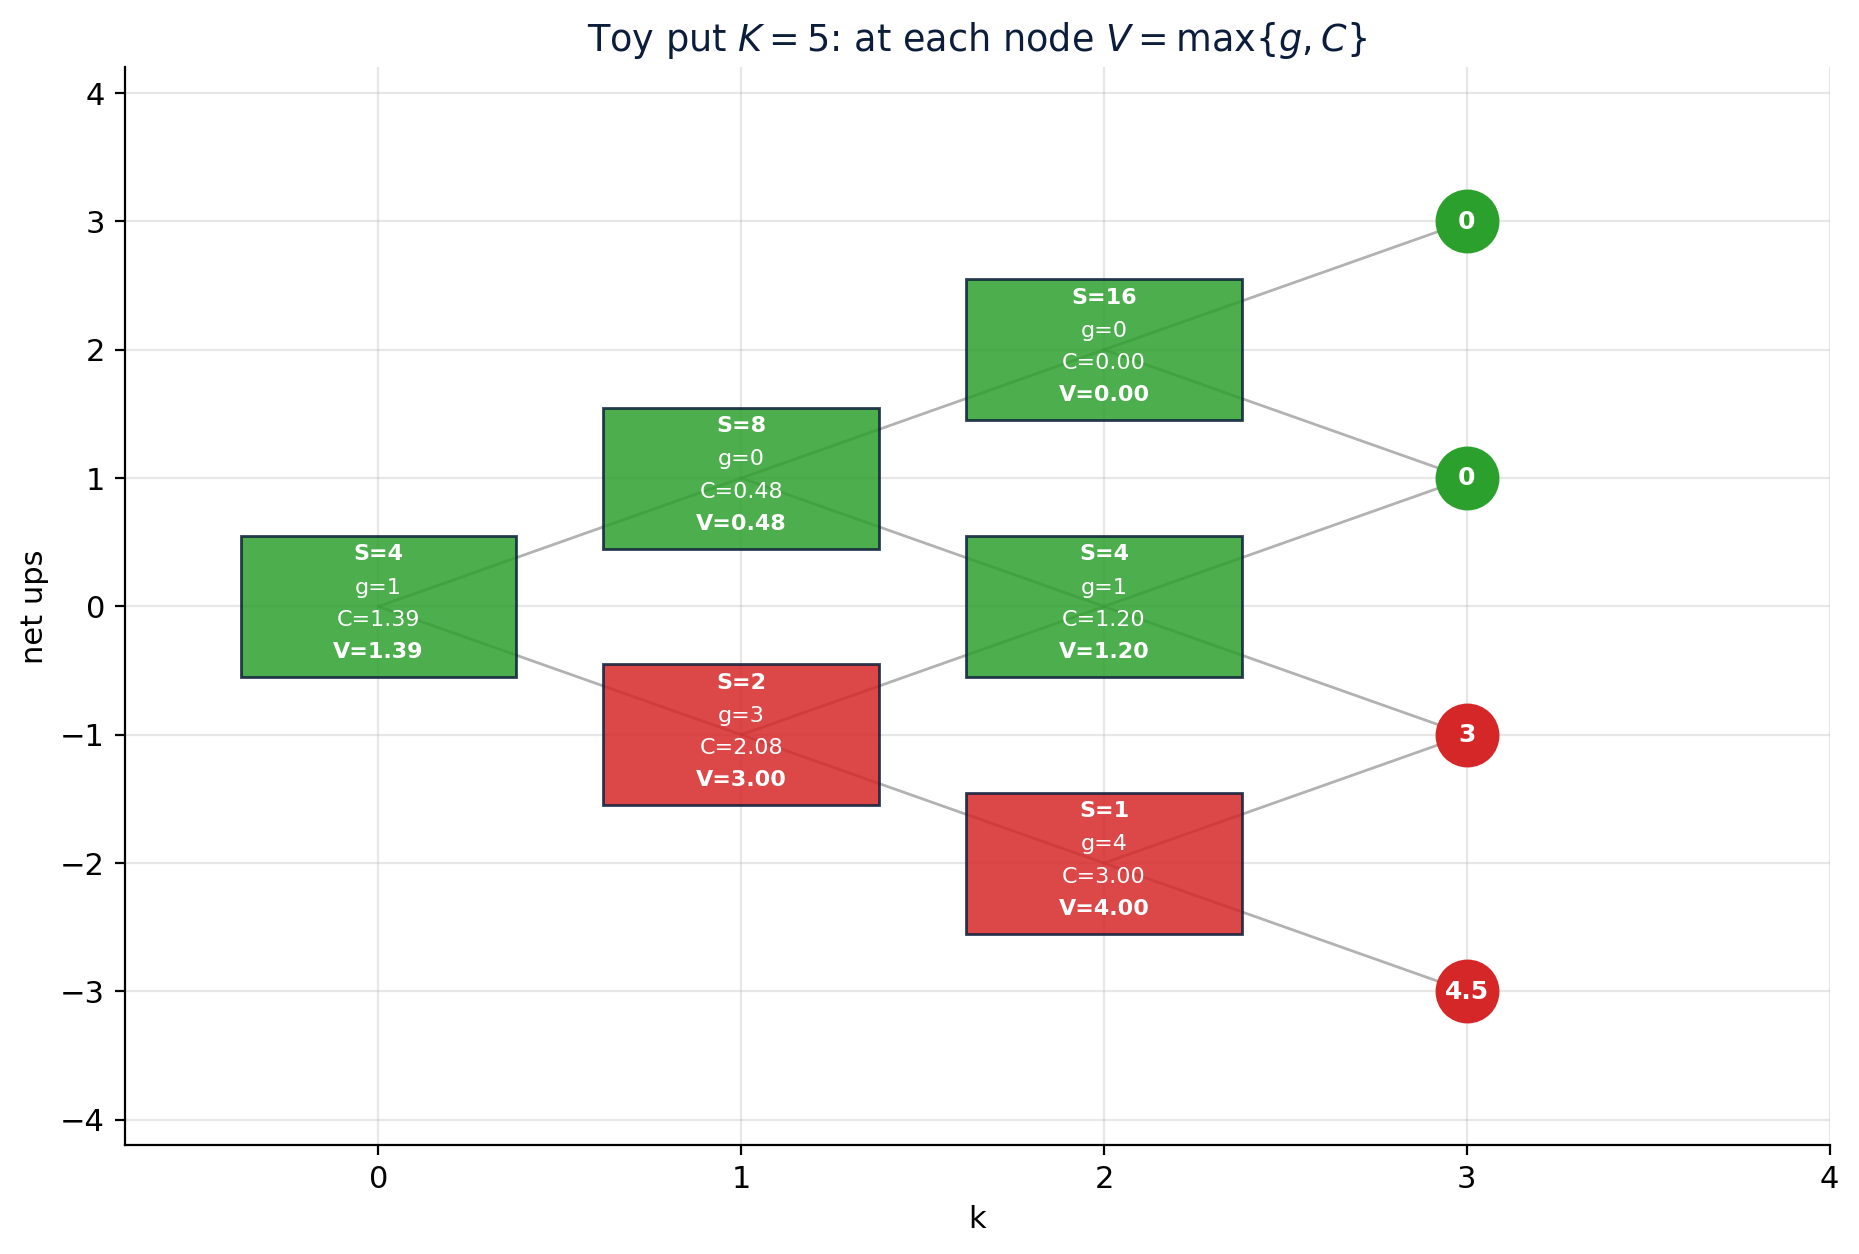
\includegraphics[keepaspectratio]{figures/ch04-put-frontier-close.png}}
\caption{ST put \(K=5\) close-up: every non-terminal node shows \(S\),
intrinsic \(g\), continuation \(C\), and the envelope \(V\). The
decision is \(V = \max\{g, C\}\) at each node.}
\end{figure}

\begin{figure}
\centering
\pandocbounded{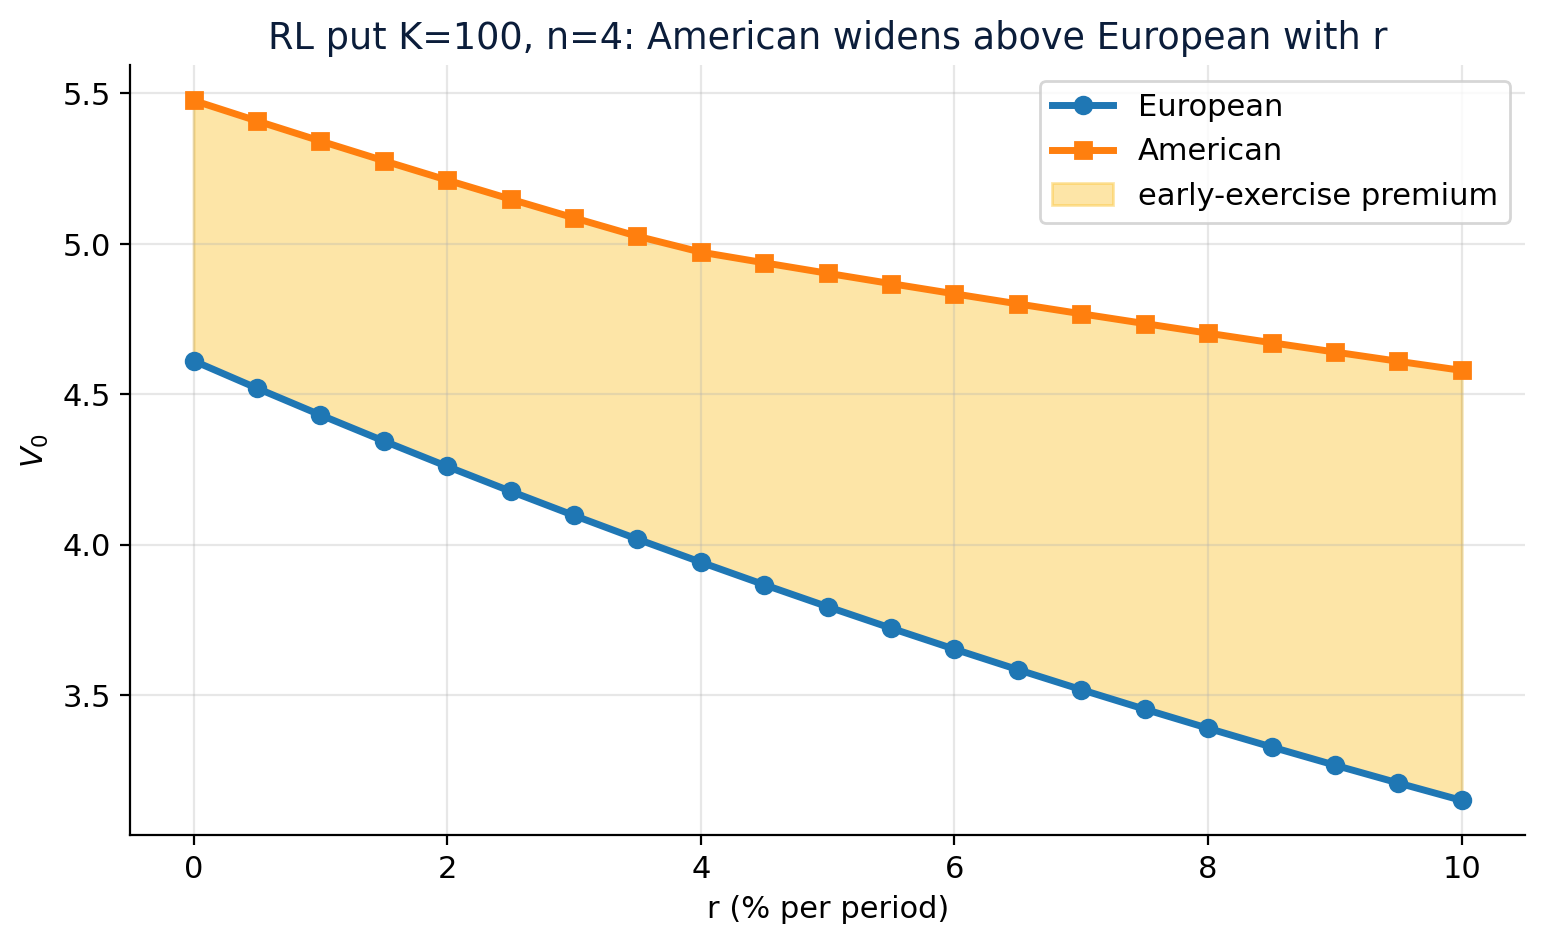
\includegraphics[keepaspectratio]{figures/ch04-V0-vs-r.png}}
\caption{\(V_0\) as a function of \(r\) for the RL put \(K=100, n=4\):
American (orange) widens away from European (blue) as \(r\) rises. The
gold band is the early-exercise premium.}
\end{figure}

\begin{figure}
\centering
\pandocbounded{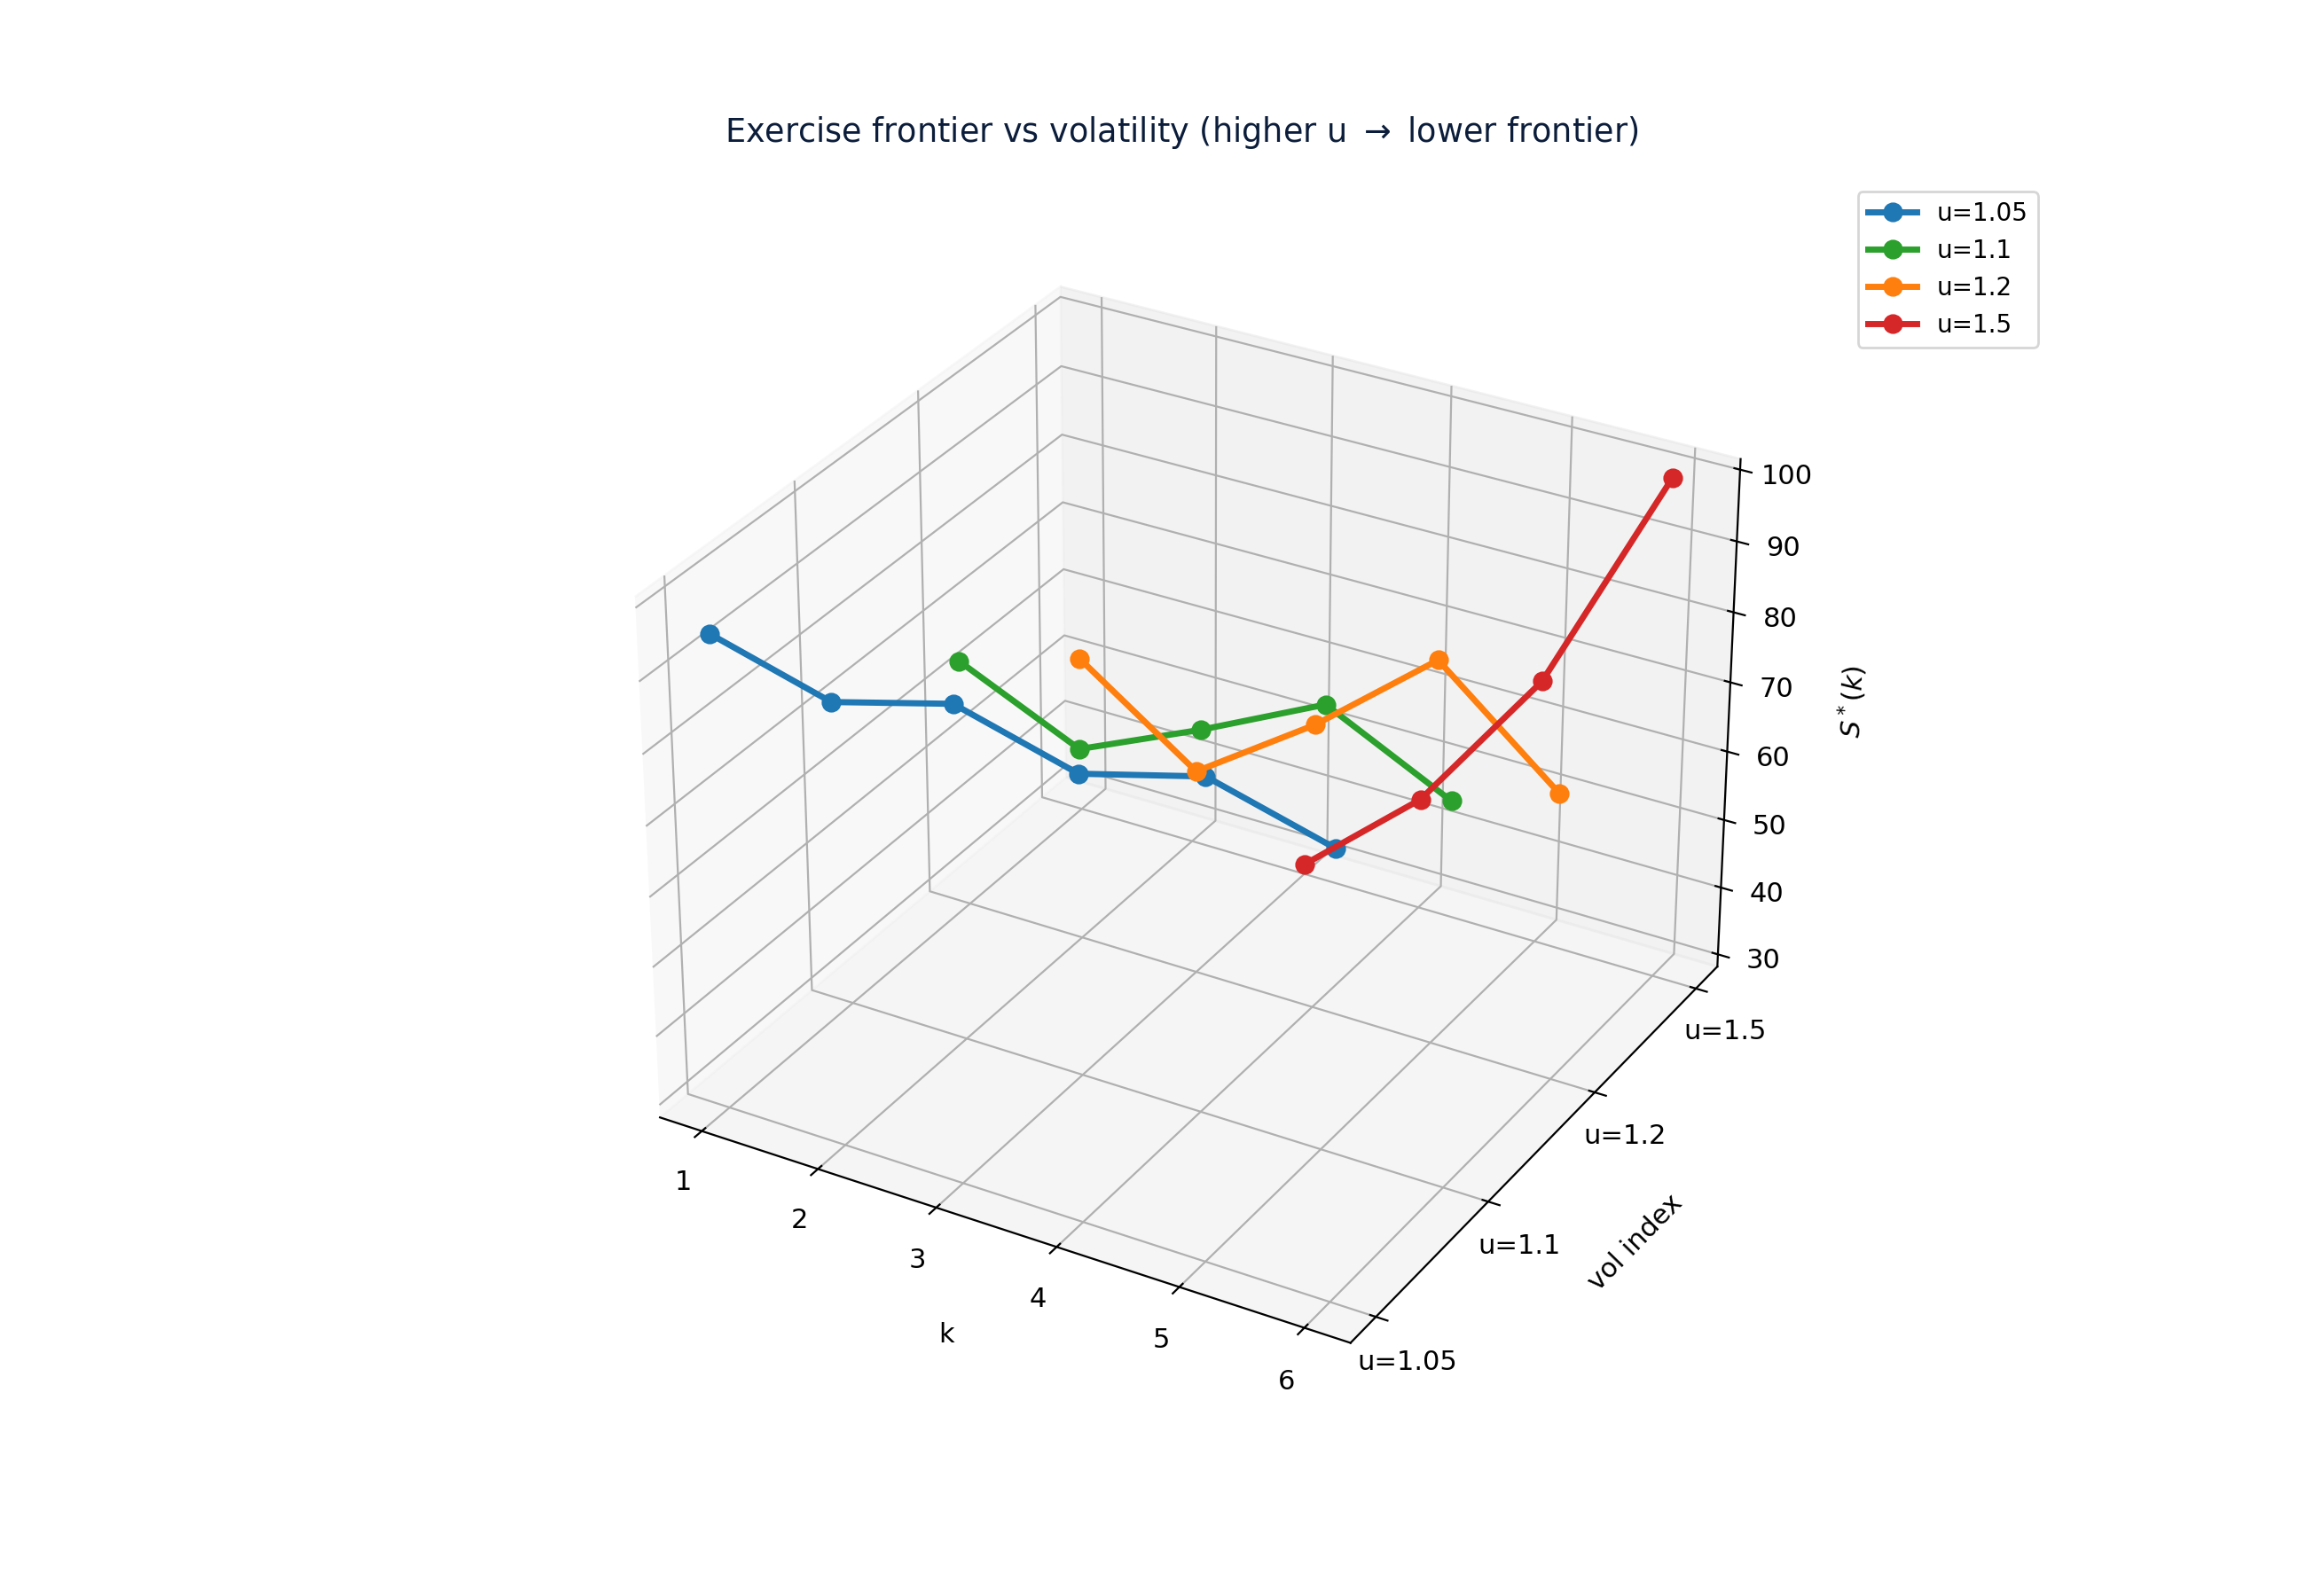
\includegraphics[keepaspectratio]{figures/ch04-frontier-sigma-3d.png}}
\caption{3-D plot of exercise frontiers \(S^*(k)\) for four volatility
levels \(u \in \{1.05, 1.10, 1.20, 1.50\}\). Higher vol → frontier sits
lower → smaller exercise region.}
\end{figure}

\subsection{4.7.3 Tables}\label{tables-10}

\textbf{Table 4.11.} \(V_0^{\text{Am put}}\) vs \(V_0^{\text{Eu put}}\)
on RL lattice \(K=100, n=4\) as a function of \(r\).

(Reproduced from Example 4.7.3.)

\textbf{Table 4.12.} ST put \(K = 5\) exercise nodes with intrinsic and
continuation values.

{\def\LTcaptype{none} % do not increment counter
\begin{table}[H]
\centering
\begin{tabular}{|c|r|r|r|c|}
\toprule
node & \(S\) & \(g\) & continuation \(C\) & exercise? \\
\midrule



\((0,0)\) & \(\phantom{0}4\) & \(1\) & \(1.36\) & no \\
\((1,1)\) & \(\phantom{0}8\) & \(0\) & \(0.40\) & no \\
\((1,0)\) & \(\phantom{0}2\) & \(3\) & \(2.00\) & \textbf{yes} \\
\((2,0)\) & \(\phantom{0}1\) & \(4\) & (n/a) & trivially \\
\((2,1)\) & \(\phantom{0}4\) & \(1\) & (n/a) & trivially \\
\((2,2)\) & \(16\) & \(0\) & (n/a) & no \\
\bottomrule
\end{tabular}
\end{table}
}

\begin{center}\rule{0.5\linewidth}{0.5pt}\end{center}

\section{§4.8 American digital, knockout, chooser,
range-accrual}\label{american-digital-knockout-chooser-range-accrual}

\textbf{Punchline.} The Snell-envelope recipe works for \emph{any}
payoff \(g\). The buyer compares intrinsic to discounted-expected
continuation at every node; the optimal exercise rule is the first
touch.

\textbf{Intuition.} The Snell envelope is a \emph{general}
dynamic-programming construct. It cares only about: (a) the intrinsic
payoff \(g\) at each node, (b) the transition probabilities to children.
Whether \(g\) is a put, a call, an indicator, or some path-dependent
function makes no structural difference --- what changes is what we plug
in for \(g\).

\subsection{4.8.1 American digital}\label{american-digital}

\textbf{Example 4.8.1 (ST American digital, \(H = 8\)).} Payoff:
\(g(s) = \mathbf{1}_{s \ge 8}\). With the toy lattice, \(S\) reaches or
exceeds \(8\) at nodes \((1, 1), (2, 2)\) (also \((2, 1)\) has
\(S = 4 < 8\)).

Backward induction:

\begin{itemize}
\tightlist
\item
  \(V_2(HH) = \mathbf{1}_{16 \ge 8} = 1\).
  \(V_2(HT) = V_2(TH) = \mathbf{1}_{4\ge 8} = 0\). \(V_2(TT) = 0\).
\item
  \(V_1(H), S = 8\): intrinsic \(1\). Continuation:
  \(\beta\cdot\tfrac{1}{2}(1 + 0) = 0.40\).
  \(V_1(H) = \max\{1, 0.40\} = 1\) → \textbf{exercise}.
\item
  \(V_1(T), S = 2\): intrinsic \(0\). Continuation:
  \(\beta\cdot\tfrac{1}{2}(0 + 0) = 0\). \(V_1(T) = 0\).
\item
  \(V_0\): intrinsic \(0\). Continuation:
  \(\beta\cdot\tfrac{1}{2}(1 + 0) = 0.40\). \(V_0 = 0.40\).
\end{itemize}

The American digital pays \(0.40\). European digital would pay
\(\beta^2\cdot\tilde{\mathbb{P}}(S_2 \ge 8) = 0.64\cdot 0.25 = 0.16\).
The American is \textbf{2.5× more valuable} than the European because it
can lock in the digital payoff as soon as \(S\) touches the threshold.

\subsection{4.8.2 American up-and-out
put}\label{american-up-and-out-put}

\textbf{Example 4.8.2 (ST American up-and-out put, \(K = 5, B = 8\)).}
Payoff: \(g(s) = (K - s)^+\) as long as the path has not touched \(B\).
The state is \((k, S_k, \mathbf{1}_{\text{touched}})\).

On the toy lattice:

\begin{itemize}
\tightlist
\item
  Path HH: \(S = 4 \to 8 \to 16\) --- touches \(B\) at \(k = 1\).
  Knocked out.
\item
  Path HT: \(S = 4 \to 8 \to 4\) --- touches at \(k = 1\). Knocked out.
\item
  Path TH: \(S = 4 \to 2 \to 4\) --- never touches.
\item
  Path TT: \(S = 4 \to 2 \to 1\) --- never touches.
\end{itemize}

For paths HH and HT, \(V = 0\) from \(k=1\) onwards.

For path TH: at \((2, 1)\) via TH, alive, \(g = 1\).
\(V_{(2,1, \text{alive})} = 1\) at terminal.

For path TT: at \((2, 0)\) alive, \(g = 4\). \(V = 4\).

Backward at \(k = 1\): - \((1, 1)\) HIT --- \(V = 0\). - \((1, 0)\)
alive, \(S = 2\), \(g = 3\). Continuation: from \((1, 0)\) the
next-period nodes are \((2, 1)\) (via T-H = TH-path = alive) with
\(V = 1\), and \((2, 0)\) (via T-T = TT, alive) with \(V = 4\). So
\(\text{cont} = \beta\cdot\tfrac{1}{2}(1 + 4) = 2\).
\(V_{(1, 0)} = \max\{3, 2\} = 3\) → \textbf{exercise}.

Backward at root: - \(V_0\): intrinsic \(1\). Continuation:
\(\beta\cdot\tfrac{1}{2}(V_{(1,1, \text{HIT})} + V_{(1, 0, \text{alive})}) = 0.8\cdot 0.5\cdot(0 + 3) = 1.20\).
\(V_0 = \max\{1, 1.20\} = 1.20\).

So the up-and-out put \(K=5, B=8\) is worth \(1.20\) --- substantially
less than the vanilla put \(1.36\), because the up branch destroys
value.

\subsection{4.8.3 American knock-in call}\label{american-knock-in-call}

\textbf{Example 4.8.3 (ST American up-and-in call, \(K = 5, B = 8\)).}
Payoff: \(g(s) = (s - K)^+\) but only after the path has touched \(B\).

\begin{itemize}
\tightlist
\item
  Paths HH, HT: touch at \(k = 1\), become live.
\item
  Paths TH, TT: never touch. Worthless.
\end{itemize}

For touched paths the contract becomes a standard American call from the
touch time onwards. From \((1, 1)\) with \(S = 8\), intrinsic \(3\),
going forward as a standard call: by §4.6 the American call equals the
European, so \(V_{(1, 1, \text{touched})}\) = European call value from
\((1, 1)\) = \(\beta\cdot\tfrac{1}{2}(11 + 0) = 4.40\).

For untouched paths, \(V\) = 0 always.

\(V_0 = \beta\cdot\tfrac{1}{2}\cdot 4.40 + \beta\cdot\tfrac{1}{2}\cdot 0 = 1.76\).

So American knock-in call = \(1.76\). Compare: vanilla American call
\(K=5\) = \(1.76\). They match! Because the only way to land at a
positive call payoff at \(k=2\) is via path HH (the only one with
\(S_2 \ge K\)), and that path has already touched \(B\) --- so the
knock-in adds no constraint.

\subsection{4.8.4 American chooser}\label{american-chooser}

\textbf{Example 4.8.4 (ST American chooser, choose at \(T_c = 1\),
mature at \(T = 2\), \(K = 5\)).} At \(k = 1\) the holder picks call or
put with strike \(K = 5\), then the option runs European to \(T = 2\).
Strictly speaking this is a Bermudan-style ``pick once'' feature, not
full path-by-path Americanness. Compute:

European call value at \((1, 1)\) (\(S = 8\)):
\(\beta\cdot\tfrac{1}{2}(11 + 0) = 4.40\). European put value:
\(\beta\cdot\tfrac{1}{2}(0 + 1) = 0.40\).

European call at \((1, 0)\) (\(S = 2\)):
\(\beta\cdot\tfrac{1}{2}(0 + 0) = 0\). European put:
\(\beta\cdot\tfrac{1}{2}(1 + 4) = 2.00\).

Chooser values at \(k = 1\): - \((1, 1)\): \(\max\{4.40, 0.40\} = 4.40\)
(pick call). - \((1, 0)\): \(\max\{0, 2.00\} = 2.00\) (pick put).

Chooser at root:
\(V_0 = \beta\cdot\tfrac{1}{2}(4.40 + 2.00) = 0.8\cdot 3.20 = 2.56\).

So the chooser is worth \(2.56\) --- strictly more than either vanilla
European call (\(1.76\)) or vanilla European put (\(0.96\)), as you'd
expect from a contract that lets you delay the call/put decision.

\subsection{4.8.5 Range-accrual American}\label{range-accrual-american}

\textbf{Example 4.8.5 (ST American range-accrual).} Payoff:
\(g_k = \#\{0 \le j \le k : a \le S_j \le b\}\) for chosen \([a, b]\).
With \([a, b] = [3, 9]\) on the toy lattice, intrinsic counts visits to
the range \(\{3, \dots, 9\}\). \(S\) values touching this range:
\(S_0 = 4, S_1 = 8, S_2 = 4\). Recompute:

\begin{itemize}
\tightlist
\item
  At \((2, 1)\): \$g = \$ count along path HT or TH of visits to
  \([3, 9]\) --- \(\{4, 8, 4\}\) on HT (3 visits), \(\{4, 2, 4\}\) on TH
  (2 visits since 2 is outside). For Snell to work cleanly we need to
  track the count: the state is \((k, S_k, \text{count}_k)\). The
  augmented state space is bigger. We'll defer further details to §4.11.
\end{itemize}

The structural point: any payoff can be Snell-priced as long as we carry
enough state.

\begin{figure}
\centering
\pandocbounded{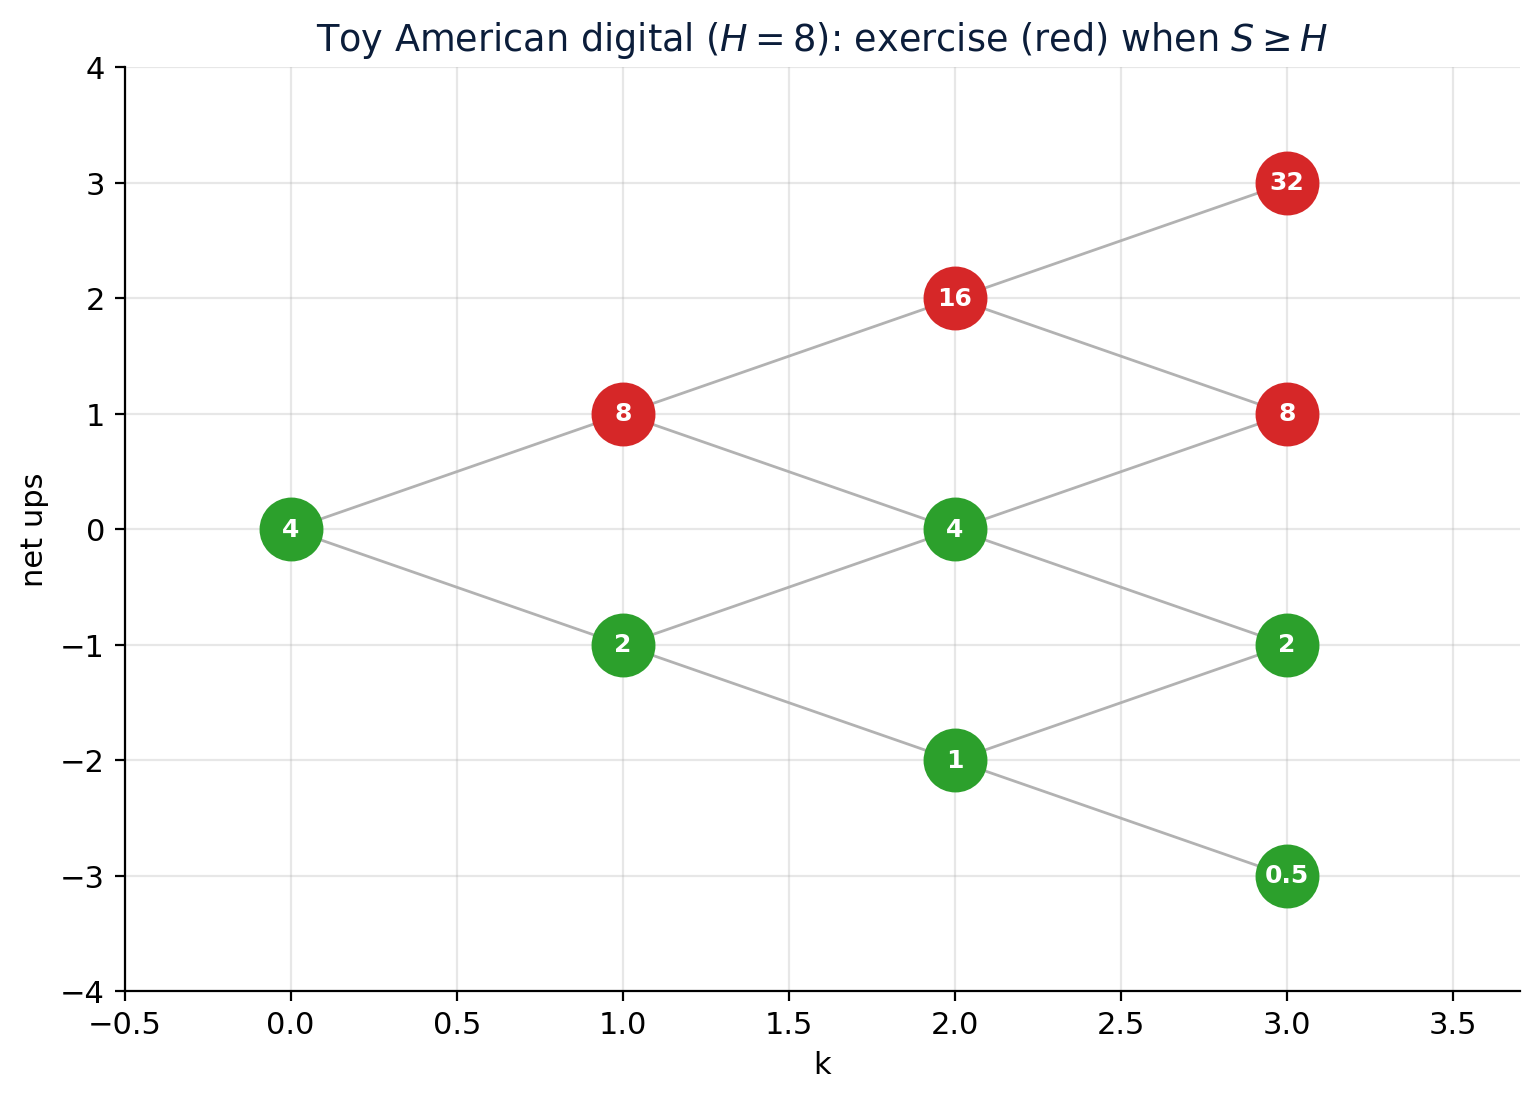
\includegraphics[keepaspectratio]{figures/ch04-digital-am.png}}
\caption{ST American digital tree (\(H = 8\)): exercise (red) the moment
\(S \ge H\).}
\end{figure}

\begin{figure}
\centering
\pandocbounded{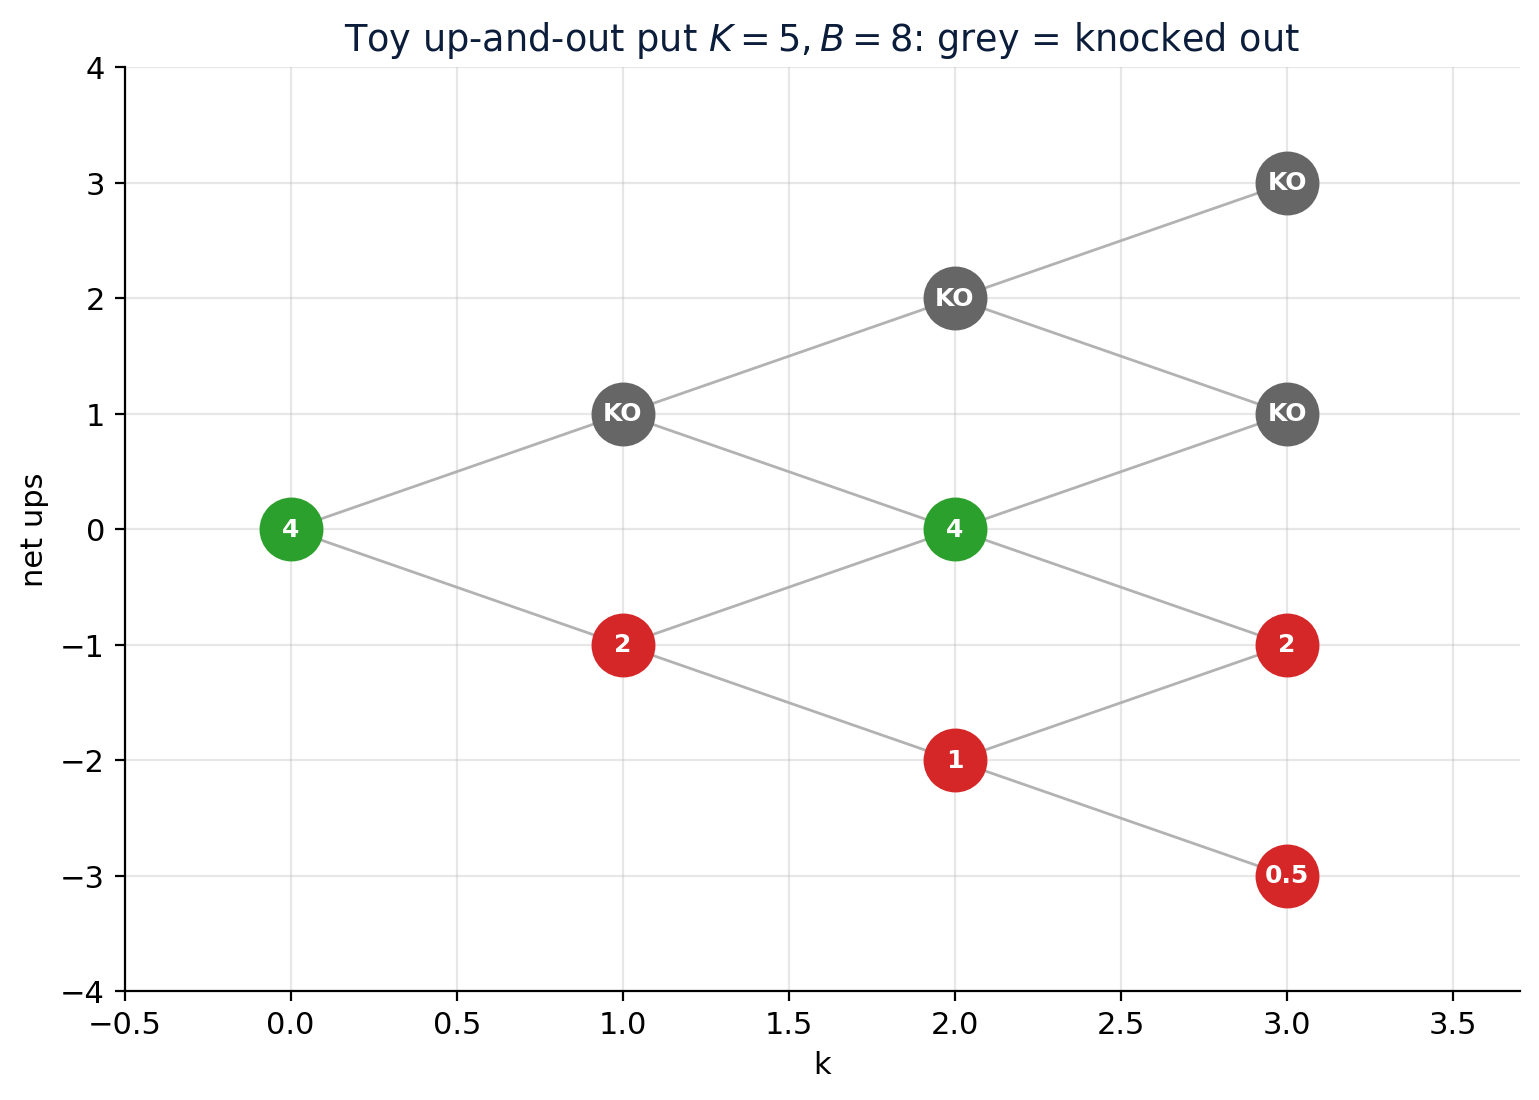
\includegraphics[keepaspectratio]{figures/ch04-knockout-am.png}}
\caption{ST American up-and-out put (\(K = 5, B = 8\)): knocked-out
nodes (grey) carry zero value; alive nodes follow standard Snell.}
\end{figure}

\begin{figure}
\centering
\pandocbounded{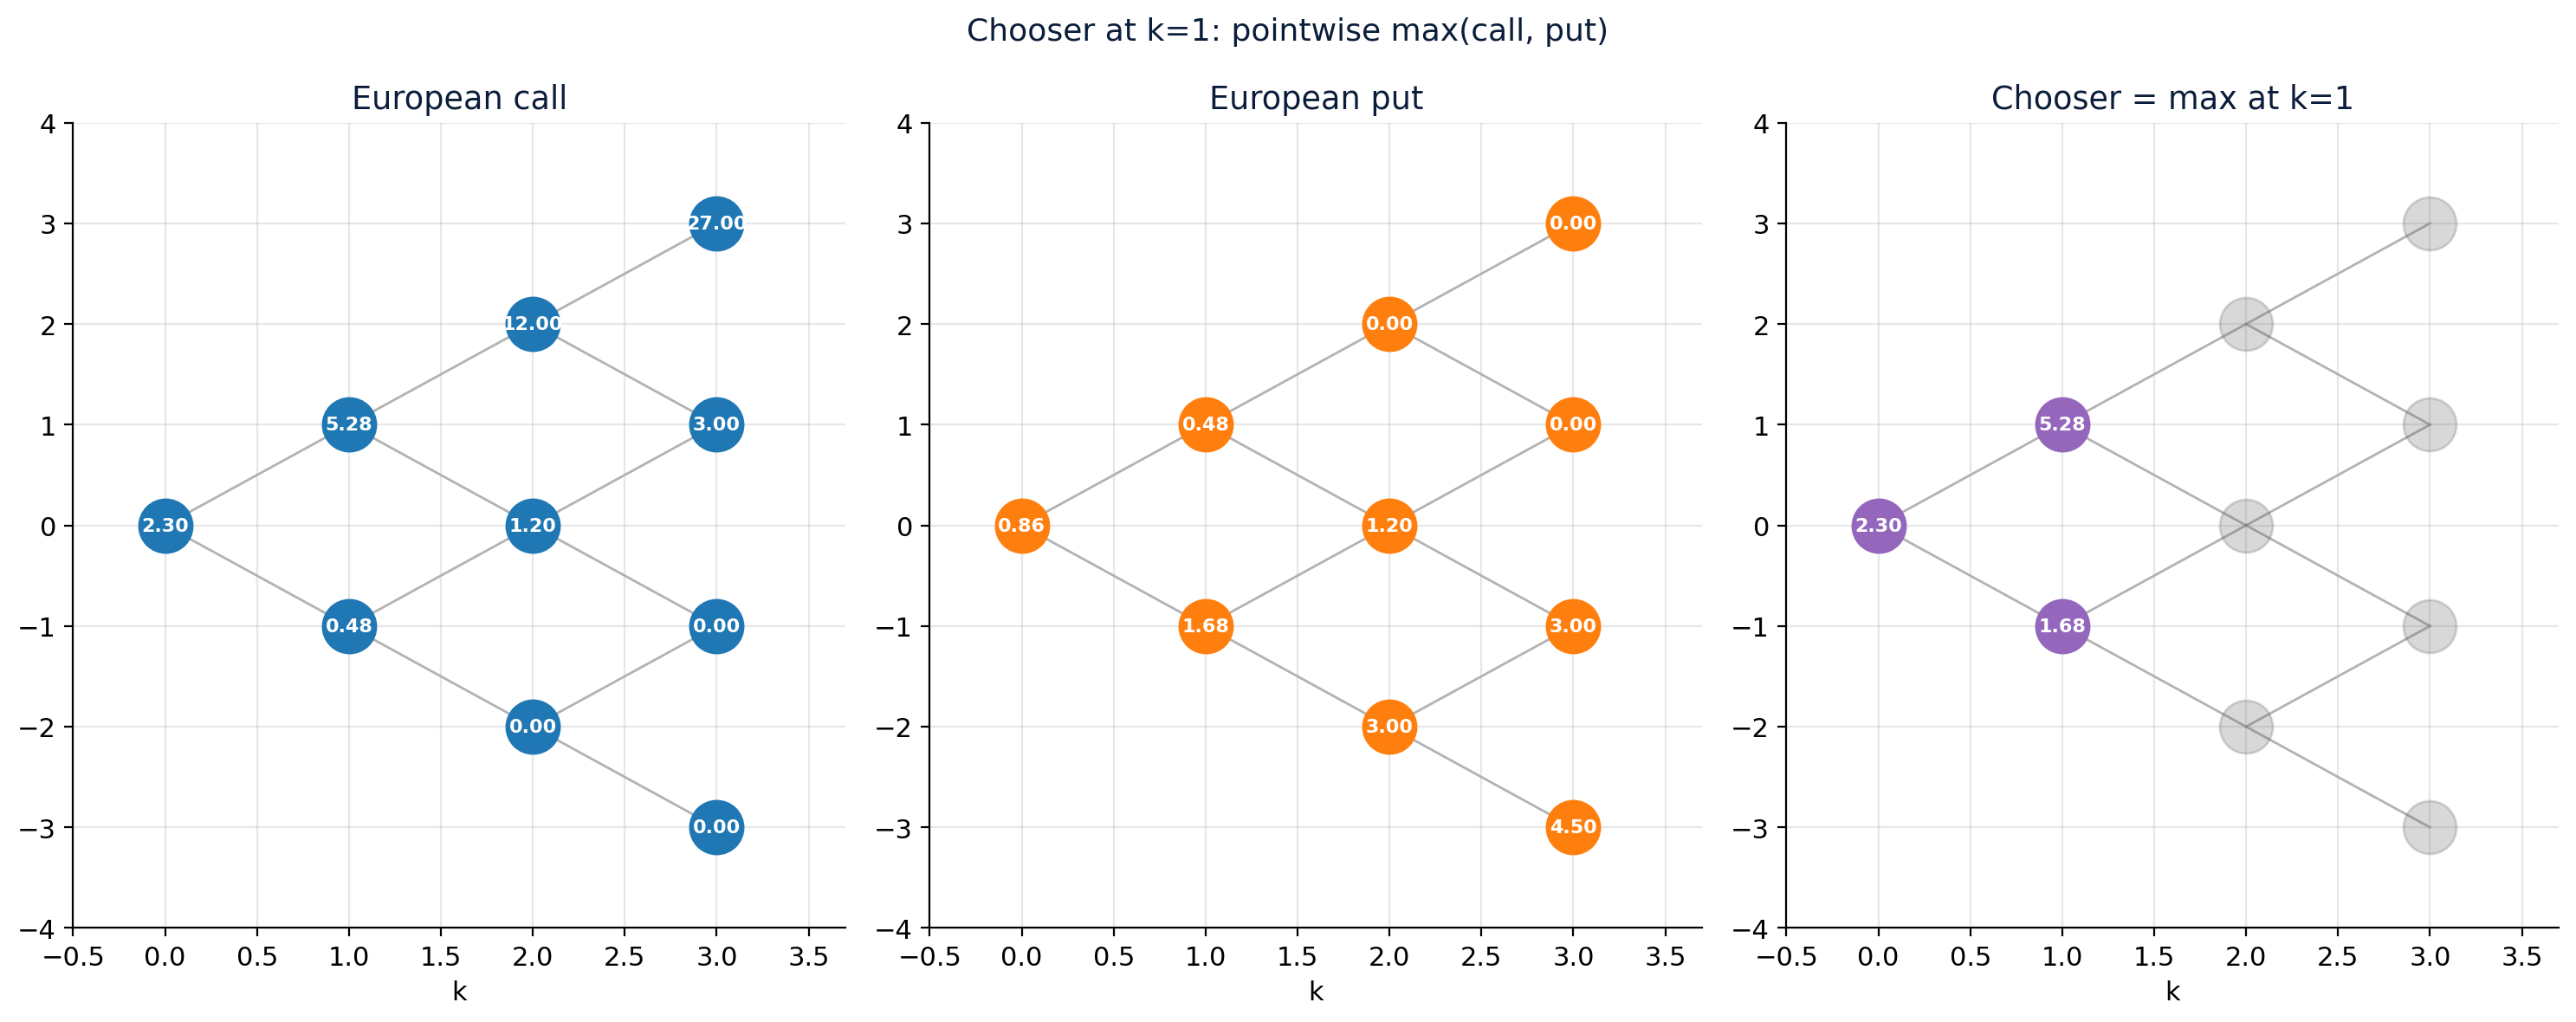
\includegraphics[keepaspectratio]{figures/ch04-chooser.png}}
\caption{Chooser decomposition: European call tree, European put tree,
and chooser = pointwise max at \(k = 1\).}
\end{figure}

\subsection{4.8.6 Table}\label{table-18}

\textbf{Table 4.13.} Five American exotic prices on the ST lattice,
compared to their European counterparts.

{\def\LTcaptype{none} % do not increment counter
\begin{table}[H]
\centering
\begin{tabular}{|l|r|r|r|}
\toprule
contract & \(V_0^{\text{Am}}\) & \(V_0^{\text{Eu}}\) & gap \\
\midrule



Vanilla put \(K = 5\) & \(1.36\) & \(0.96\) & \(0.40\) \\
Vanilla call \(K = 5\) & \(1.76\) & \(1.76\) & \(0.00\) \\
Digital \(H = 8\) & \(0.40\) & \(0.16\) & \(0.24\) \\
Up-and-out put \(K=5, B=8\) & \(1.20\) & \(0.96\) & \(0.24\) \\
Up-and-in call \(K=5, B=8\) & \(1.76\) & \(1.76\) & \(0.00\) \\
Chooser \(T_c=1\) & \(2.56\) & \(2.56\) & \(0.00\) \\
\bottomrule
\end{tabular}
\end{table}
}

(Numerical values are the ones computed in Examples 4.8.1 -- 4.8.4.)

\begin{center}\rule{0.5\linewidth}{0.5pt}\end{center}

\section{§4.9 Hedging American options ---
super-replication}\label{hedging-american-options-super-replication}

\textbf{Punchline.} The dealer who sold an American option hedges by
\textbf{super-replicating}: maintain a portfolio whose wealth \(X_k\)
satisfies \(X_k \ge g(S_k)\) at \emph{every} node, on \emph{every} path.
The required initial wealth is exactly \(V_0\). The hedge consumes a
non-negative \textbf{consumption process} \(\{dC_k\}\) at nodes where
the supermartingale would lose slack --- these are the nodes the holder
would have optimally exercised at.

\textbf{Intuition.} Selling a European option, the dealer's hedge is
\emph{exactly} a replicating portfolio: wealth tracks the option value.
Selling an American, the dealer doesn't know when the buyer will
exercise --- so she must be \emph{prepared} to deliver intrinsic at
every node. Her wealth must dominate intrinsic everywhere. The Snell
envelope \(V\) is precisely the smallest wealth process that does so,
and the consumption \(dC\) is the cash the dealer is \emph{forced} to
set aside (or ``consume'') at exercise-region nodes.

\subsection{4.9.1 The hedging recursion}\label{the-hedging-recursion}

Let \(V_k\) be the Snell envelope. Define the dealer's hedge as follows.
At time \(k\) at node with current spot \(S_k\):

\begin{enumerate}
\def\labelenumi{\arabic{enumi}.}
\tightlist
\item
  Compute the continuation value
  \(c_k := \beta\tilde{\mathbb{E}}[V_{k+1}\mid\mathcal F_k]\).
\item
  Set up a one-period replication for \(c_k\) (the standard
  \(\Delta_k, B_k\) from Ch 1):
  \[\Delta_k := \frac{V_{k+1}^{\text{up}} - V_{k+1}^{\text{down}}}{S_{k+1}^{\text{up}} - S_{k+1}^{\text{down}}}.\]
\item
  Withdraw consumption: \(dC_k := V_k - c_k \ge 0\). This is zero on
  continuation nodes and positive (= early-exercise premium) on exercise
  nodes.
\end{enumerate}

After the move from \(k\) to \(k+1\), dealer's wealth is
\[X_{k+1} = \Delta_k S_{k+1} + (1+r)(X_k - dC_k - \Delta_k S_k).\]

Setting \(X_0 = V_0\) and applying the one-step replication,
\(X_k = V_k\) at every node. Combined with \(V_k \ge g(S_k)\) (the Snell
domination), this gives \(X_k \ge g(S_k)\) everywhere:
\textbf{super-replication}.

\subsection{\texorpdfstring{4.9.2 Worked example --- ST put
\(K = 5\)}{4.9.2 Worked example --- ST put K = 5}}\label{worked-example-st-put-k-5}

\textbf{Example 4.9.1 (hedge schedule).} With \(V\) from §4.3.2:

Compute deltas at each non-terminal node:

\begin{itemize}
\tightlist
\item
  \(\Delta_0 = (V_1(H) - V_1(T))/(S_1(H) - S_1(T)) = (0.40 - 3)/(8 - 2) = -2.60/6 = -0.4333\).
\item
  \(\Delta_1(H) = (V_2(HH) - V_2(HT))/(S_2(HH) - S_2(HT)) = (0 - 1)/(16 - 4) = -1/12 = -0.0833\).
\item
  \(\Delta_1(T) = (V_2(TH) - V_2(TT))/(S_2(TH) - S_2(TT)) = (1 - 4)/(4 - 1) = -1\).
\end{itemize}

Consumption:

\begin{itemize}
\tightlist
\item
  \(dC_0 = V_0 - c_0 = 1.36 - \beta\cdot\tfrac{1}{2}(0.40 + 3) = 1.36 - 1.36 = 0\).
\item
  \(dC_1(H) = V_1(H) - c_1(H) = 0.40 - \beta\cdot\tfrac{1}{2}(0 + 1) = 0.40 - 0.40 = 0\).
\item
  \(dC_1(T) = V_1(T) - c_1(T) = 3 - \beta\cdot\tfrac{1}{2}(1 + 4) = 3 - 2 = 1\).
\end{itemize}

The dealer consumes \(\$1\) at node \((1, T)\) --- precisely the node
where the holder optimally exercises. The dealer is \emph{forced} to set
aside this dollar because if the holder exercises here, she walks away
with \(g = 3\) and the dealer must deliver \(3\) from her portfolio.

\textbf{Example 4.9.2 (verify wealth tracks \(V\)).} Starting
\(X_0 = V_0 = 1.36\).

Path goes up to \(S_1 = 8\):
\(X_1 = \Delta_0\cdot 8 + 1.25\cdot(1.36 - 0 - \Delta_0\cdot 4) = -0.4333\cdot 8 + 1.25\cdot(1.36 - (-0.4333\cdot 4)) = -3.467 + 1.25\cdot(1.36 + 1.733) = -3.467 + 1.25\cdot 3.093 = -3.467 + 3.867 = 0.400\)
✓ Matches \(V_1(H) = 0.40\).

Path goes down to \(S_1 = 2\):
\(X_1 = -0.4333\cdot 2 + 1.25\cdot(1.36 - (-0.4333\cdot 4)) = -0.867 + 3.867 = 3.000\)
✓ Matches \(V_1(T) = 3\).

\textbf{Example 4.9.3 (holder exercises suboptimally at \((1, H)\)).}
Suppose the holder exercises at \((1, H)\) where \(g = 0\). Dealer hands
over \(0\), retains \(V_1(H) = 0.40\). Free \(0.40\) to keep (no further
exercise possible since the option's been exercised). Dealer
\textbf{profits} \(0.40\) --- the holder's mistake. This is a
sub-optimal exercise: the dealer pocketed the option's continuation
value.

\textbf{Example 4.9.4 (holder exercises at \((2, TT)\)).} From
\((1, T)\), the holder waits one more step instead of exercising
optimally. At \((2, TT)\), holder receives \(g = 4\). Did the dealer's
portfolio track?

At \((1, T)\) dealer's wealth was \(3\). Now the dealer doesn't consume
the \(1\) (because the holder didn't exercise yet), so we model: keeping
the full \(V_1(T) = 3\), set up next-period hedge.

Going \(T\) then \(T\):
\(X_2 = \Delta_1(T)\cdot 1 + 1.25\cdot(3 - 0 - \Delta_1(T)\cdot 2) = -1\cdot 1 + 1.25\cdot(3 - (-1\cdot 2)) = -1 + 1.25\cdot 5 = -1 + 6.25 = 5.25\).

But \(V_2(TT) = 4\), so the dealer has \(5.25 > 4\) --- an excess of
\(1.25\). Where does that come from? It's the \(dC_1(T) = 1\) that the
dealer \textbf{should have consumed} at \((1, T)\) but didn't because
the buyer waited --- and that dollar grew at \(r\) to \(1.25\).

So if the buyer waits past \((1, T)\), the dealer ends with a
\emph{surplus}. The dealer breaks even on path-by-path delivery and
gains the present value of any held-back consumption if the buyer is
suboptimal. \textbf{Win-win for the dealer if she's correctly priced.}

\textbf{Example 4.9.5 (if the buyer exercises optimally at \((1, T)\)).}
Wealth \(X_1(T) = 3\). Dealer pays the holder \(g(2) = 3\). Wealth after
delivery: \(0\). Contract closes. Dealer broke even. ✓

\begin{figure}
\centering
\pandocbounded{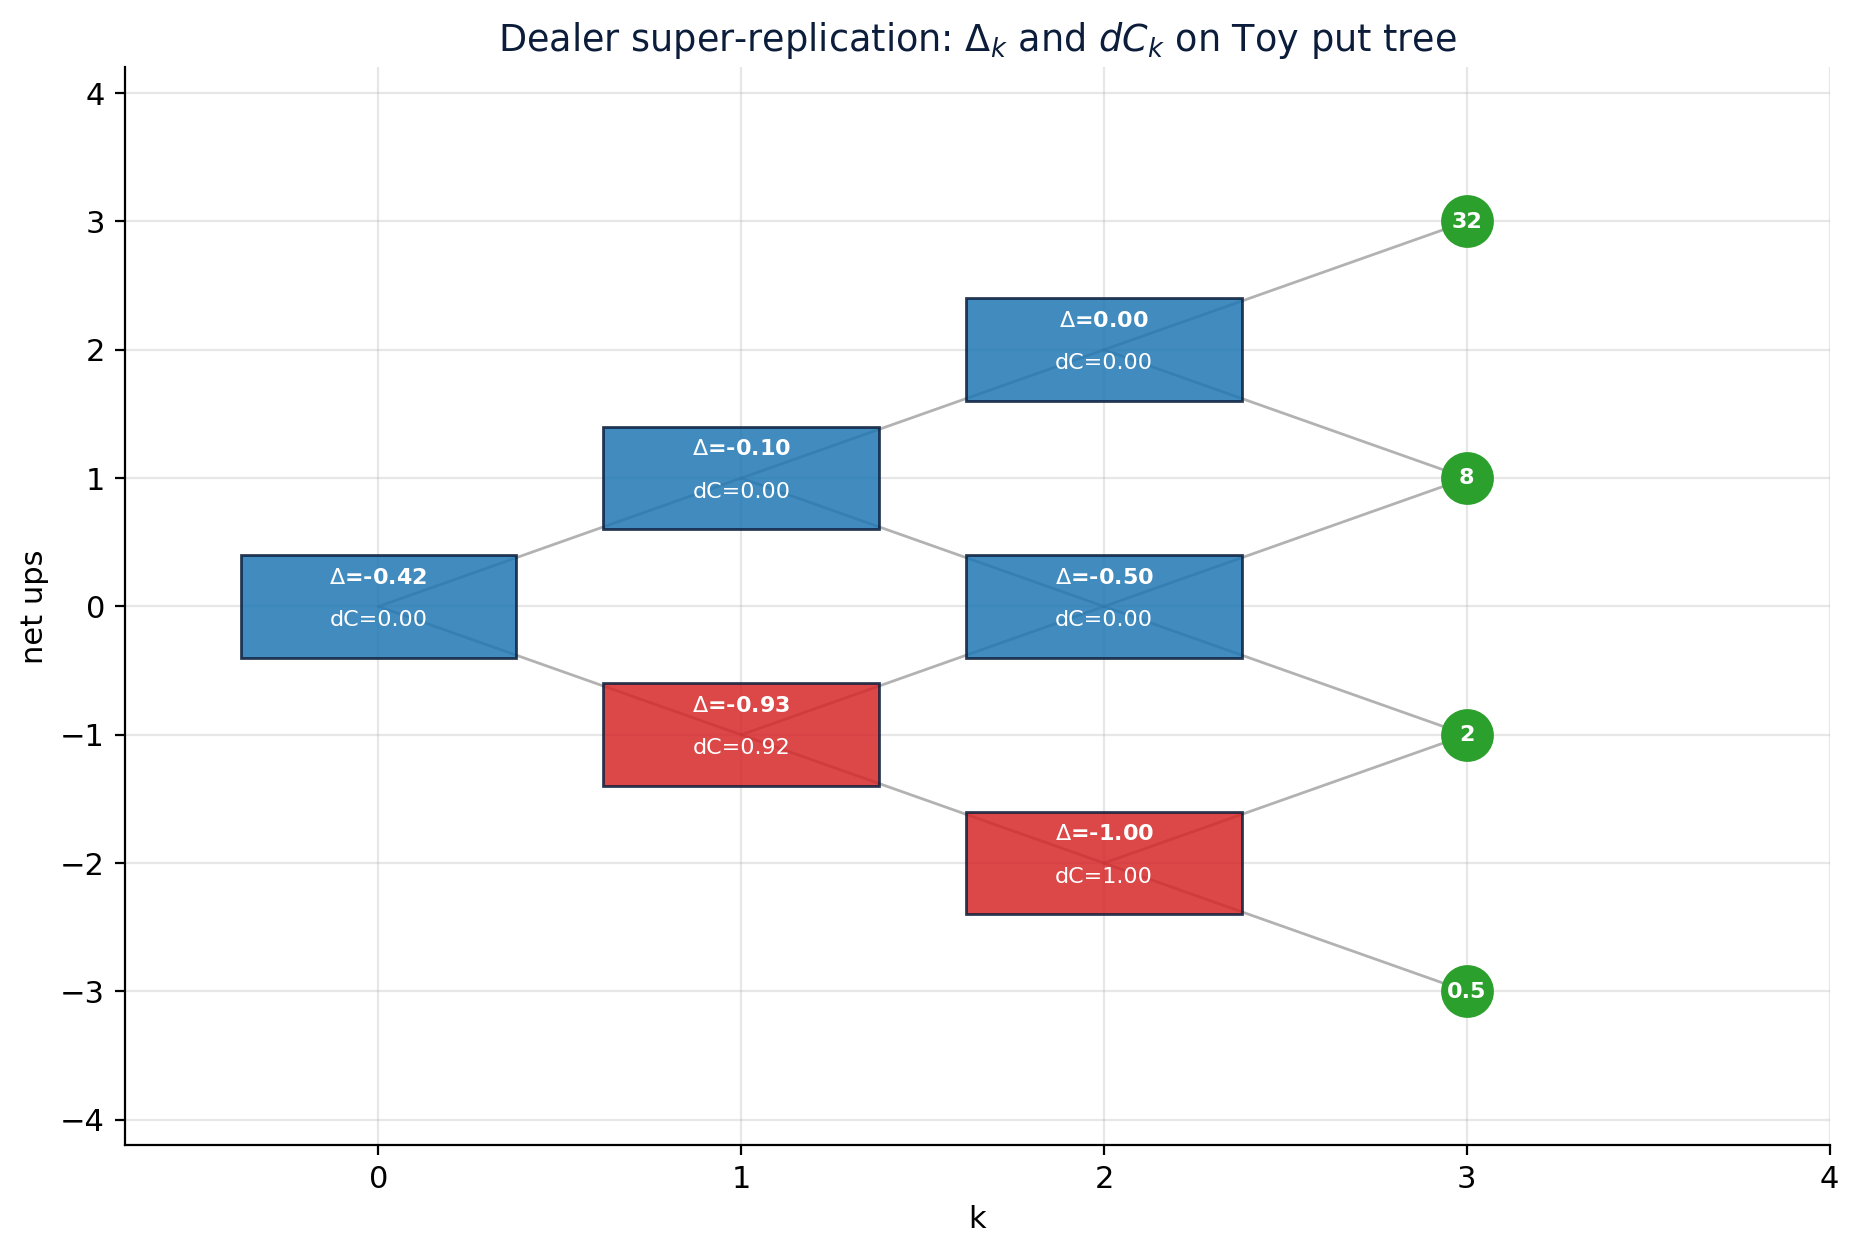
\includegraphics[keepaspectratio]{figures/ch04-delta-X-tree.png}}
\caption{Dealer's super-replication: \(\Delta_k\) shares and consumption
\(dC_k\) at each non-terminal node of the ST put \(K=5\) tree.}
\end{figure}

\begin{figure}
\centering
\pandocbounded{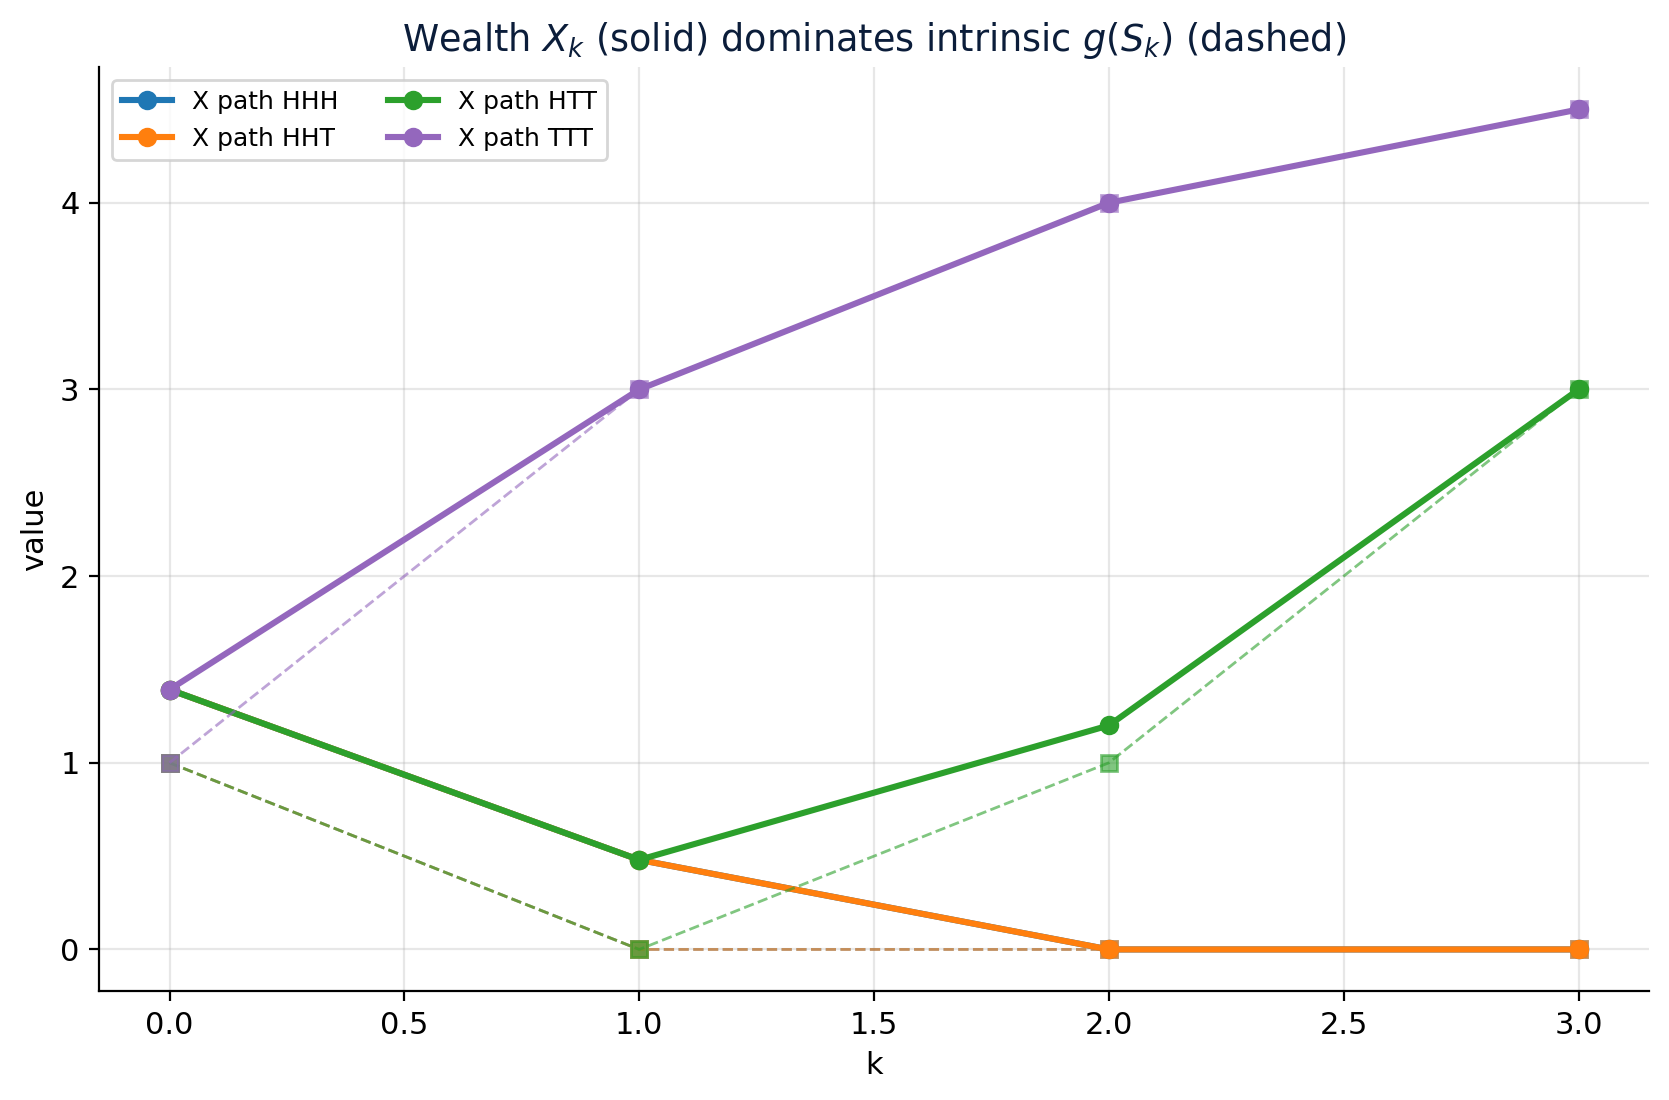
\includegraphics[keepaspectratio]{figures/ch04-X-vs-g-path.png}}
\caption{Wealth \(X_k\) (solid) and intrinsic \(g(S_k)\) (dashed) for
the dealer along all four paths. Wealth always lies above intrinsic ---
super-replication.}
\end{figure}

\begin{figure}
\centering
\pandocbounded{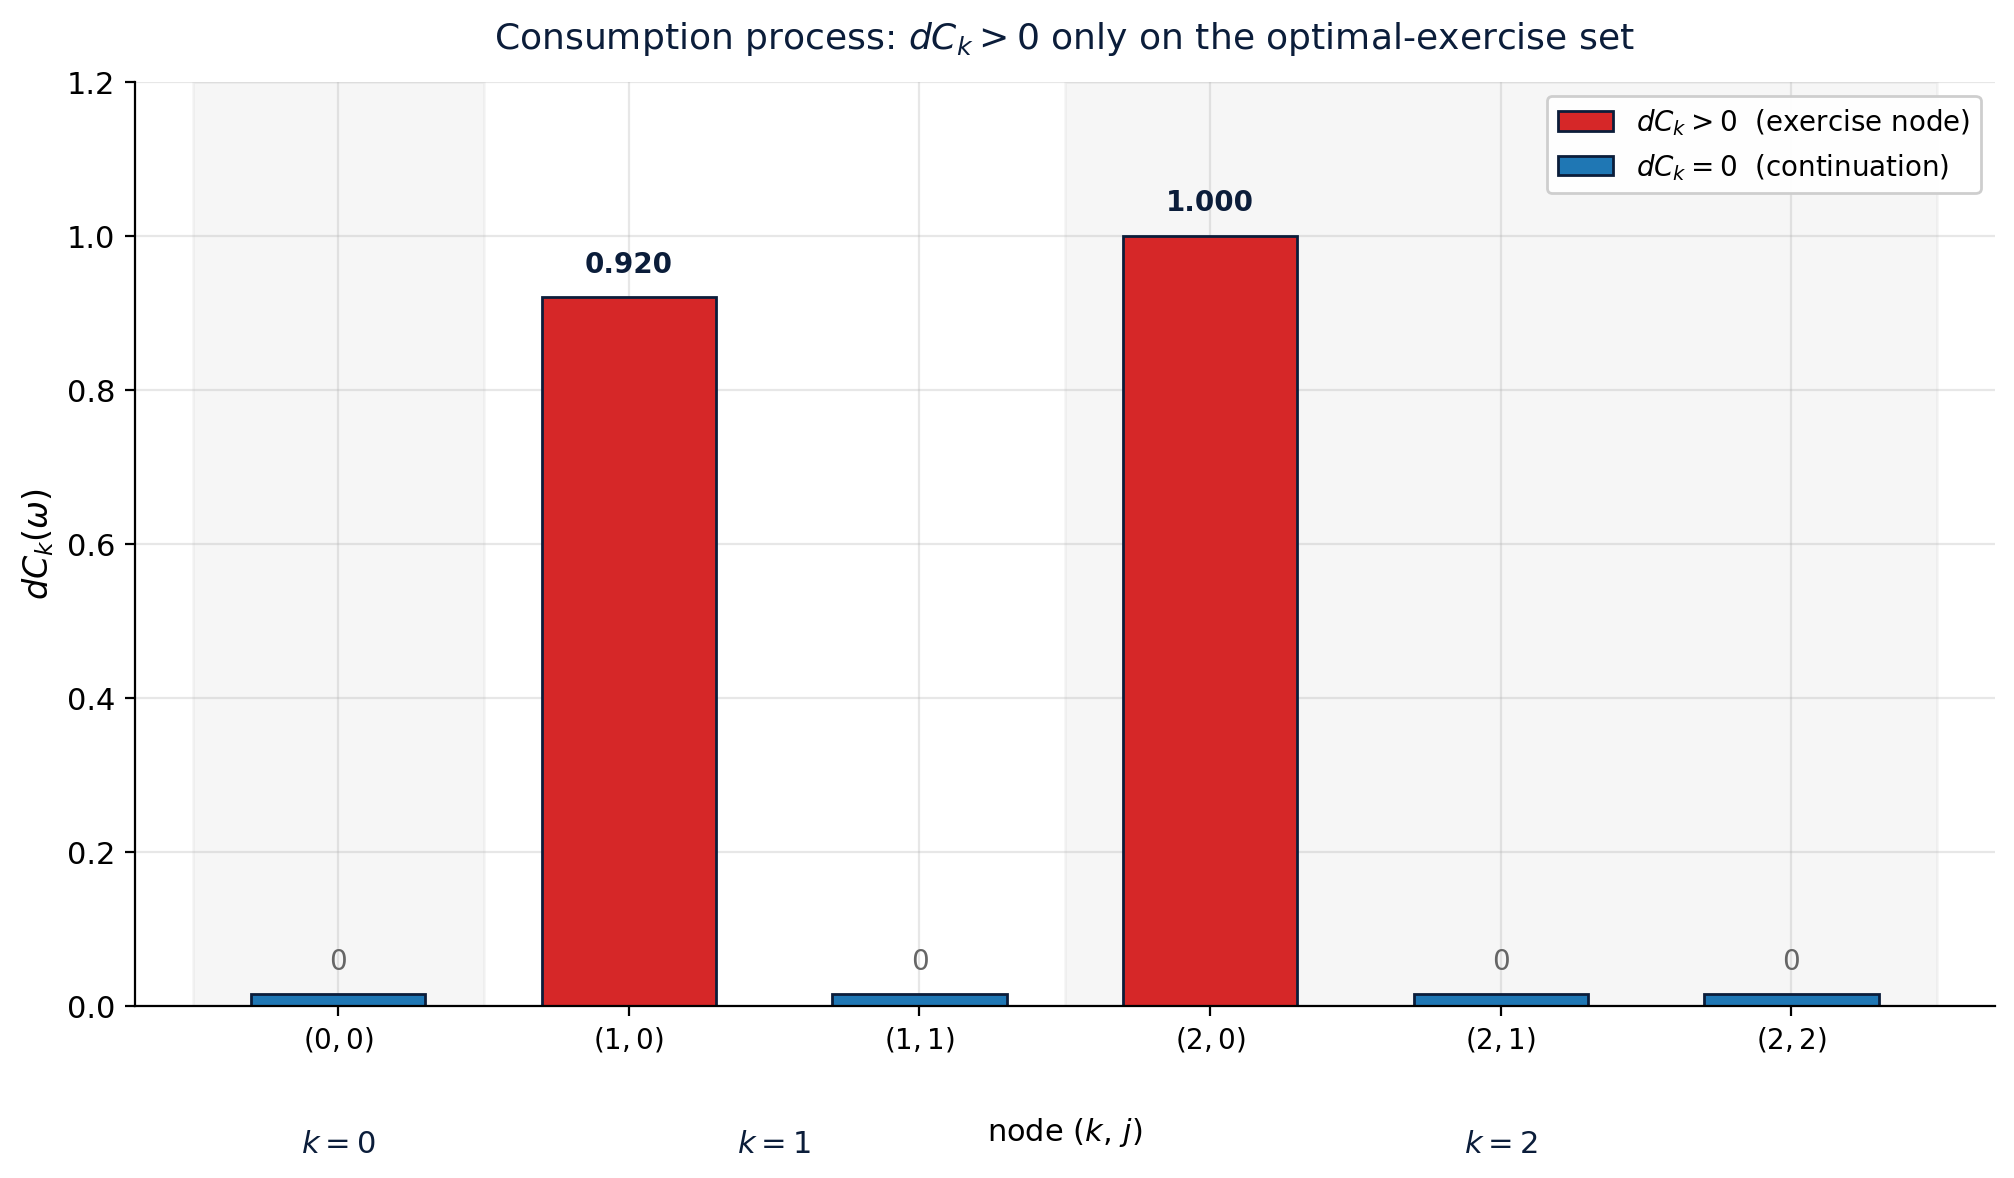
\includegraphics[keepaspectratio]{figures/ch04-consumption-bars.png}}
\caption{Consumption \(dC_k\) at each non-terminal node. Positive only
at \((1, T)\), the optimal-exercise node.}
\end{figure}

\subsection{4.9.3 Table}\label{table-19}

\textbf{Table 4.14.} Hedge schedule for the ST put \(K=5\):

{\def\LTcaptype{none} % do not increment counter
\begin{table}[H]
\centering
\begin{tabular}{|c|r|r|r|r|r|r|}
\toprule
node & \(S\) & \(V\) & \(\Delta\) & \(X\) & \(g\) & slack \(X - g\) \\
\midrule



\((0,0)\) & \(\phantom{0}4\) & \(1.36\) & \(-0.433\) & \(1.36\) & \(1\)
& \(0.36\) \\
\((1,H)\) & \(\phantom{0}8\) & \(0.40\) & \(-0.083\) & \(0.40\) & \(0\)
& \(0.40\) \\
\((1,T)\) & \(\phantom{0}2\) & \(3.00\) & \(-1.000\) & \(3.00\) & \(3\)
& \(0.00\) \\
\((2,HH)\) & \(16\) & \(0.00\) & & \(0.00\) & \(0\) & \(0.00\) \\
\((2,HT)\) & \(\phantom{0}4\) & \(1.00\) & & \(1.00\) & \(1\) &
\(0.00\) \\
\((2,TH)\) & \(\phantom{0}4\) & \(1.00\) & & \(1.00\) & \(1\) &
\(0.00\) \\
\((2,TT)\) & \(\phantom{0}1\) & \(4.00\) & & \(4.00\) & \(4\) &
\(0.00\) \\
\bottomrule
\end{tabular}
\end{table}
}

\emph{Blank: \(\Delta\) undefined at terminal nodes (no future steps to
hedge).}

Slack is the surplus the dealer carries above intrinsic. At the
optimal-exercise node \((1, T)\), slack is zero --- the buyer has no
rent left to extract.

\begin{center}\rule{0.5\linewidth}{0.5pt}\end{center}

\section{§4.10 Free lunch when American is
mispriced}\label{free-lunch-when-american-is-mispriced}

\textbf{Punchline.} If the market quotes an American option below
\(V_0\), \textbf{buy and exercise via \(\tau^*\)} --- locked-in profit
\(V_0 - P\) at \(k = 0\), plus compounded interest growth. If quoted
above \(V_0\), \textbf{sell and super-replicate} --- pocket \(P - V_0\)
at sale, with the hedge guaranteed to cover any exercise the buyer
chooses.

\textbf{Intuition.} The Snell-envelope value \(V_0\) is the
\emph{unique} no-arbitrage price for the American option. Any quoted
price away from \(V_0\) creates an arbitrage opportunity. The mechanics
for an American look just like the European case (Ch 1), with one
wrinkle: the buyer-side arbitrage uses the optimal stopping time
\(\tau^*\), and the seller-side uses the super-replicating portfolio of
§4.9.

\subsection{\texorpdfstring{4.10.1 Buyer's free lunch --- quoted below
\(V_0\)}{4.10.1 Buyer's free lunch --- quoted below V\_0}}\label{buyers-free-lunch-quoted-below-v_0}

\textbf{Example 4.10.1 (ST put quoted at \(P = 1.20\), true
\(V_0 = 1.36\)).} The dealer's quote is \(0.16\) below the true price.

\textbf{Strategy.} At \(k = 0\): 1. Borrow \(1.20\) at rate \(r\). 2.
Buy the put for \(1.20\).

Net cash: \(0\).

At \(k = 1\) on path \(T\): exercise the put, receive \(g = 3\). Pay off
the loan: \(1.20\cdot 1.25 = 1.50\). Net: \(3 - 1.50 = 1.50\).

But wait --- for this to be arbitrage we need a \emph{non-negative}
result on every path and \emph{strictly positive} with positive
probability. Path \(H\) at \(k = 1\): we have not exercised. At
\(k = 2\) on path \(HH\): \(g = 0\). We owe
\(1.20\cdot 1.25^2 = 1.875\). Net: \(-1.875\).

So this isn't quite right. We need to also short-replicate the option to
neutralise the unfavourable paths. Specifically: at \(k = 0\) buy the
option \emph{and short-sell its replicating portfolio}.

\textbf{Correct arbitrage strategy.} Buy the option for \(1.20\); sell
forward exposure equivalent to the replicating portfolio of an
\emph{American at price \(1.36\)}, holding the hedge wealth
\(X = 1.36\). Net cash position at \(k = 0\) is
\(X_0 - P = 1.36 - 1.20 = 0.16\).

Now at every future node, our hedge wealth tracks \(V_k\), and we
receive \(g(S_\tau)\) when we exercise. Choose \(\tau = \tau^*\). We owe
back the hedge wealth \(X_\tau = V_\tau = g(S_\tau)\), and receive
\(g(S_\tau)\) from exercising. Net at exercise: \(0\). Net at the start:
\(0.16\) pocketed.

Locked-in profit: \(0.16\) at \(k = 0\), no risk.

\textbf{Example 4.10.2 (RL put quoted at \(4.60\), true \(4.91\)).}
Similar arbitrage: buy at \(4.60\), hedge-short at \(4.91\), pocket
\(0.31\) now.

\subsection{\texorpdfstring{4.10.2 Dealer's free lunch --- quoted above
\(V_0\)}{4.10.2 Dealer's free lunch --- quoted above V\_0}}\label{dealers-free-lunch-quoted-above-v_0}

\textbf{Example 4.10.3 (ST put quoted at \(P = 1.50\), true
\(V_0 = 1.36\)).}

\textbf{Strategy.} Sell the option at \(1.50\). Use \(1.36\) to set up
the super-replicating portfolio (§4.9). Pocket \(0.14\) immediately,
plus invest at rate \(r\).

If the buyer exercises at \(\tau^*\) (the worst case for the dealer),
the hedge delivers exactly \(g(S_{\tau^*})\). Dealer breaks even on the
obligation but keeps the \(0.14\) initial surplus, which has grown to
\(0.14\cdot(1.25)^{\tau^*}\) in present-of-\(\tau^*\) value (or kept in
cash from \(k=0\)).

If the buyer exercises suboptimally --- say, at a continuation-region
node --- the hedge has surplus left over (slack), which the dealer also
pockets. Even better for the dealer.

\textbf{Bound on the dealer's profit.} Minimum profit:
\(1.50 - 1.36 = 0.14\). Maximum: depends on how badly the buyer
exercises.

\subsection{4.10.3 No-arbitrage band}\label{no-arbitrage-band}

In practice, transaction costs and bid-ask spreads create a
\emph{no-arbitrage band} \([V_0 - \epsilon, V_0 + \epsilon]\) within
which mispricing is not exploitable. Outside this band the strategies
above lock in profit.

\textbf{Example 4.10.4 (compare European vs American mispricing arbs).}
A European put mispriced at \(P\) vs true \(V_0^{\text{Eu}} = 0.96\)
creates arbitrage of \(|V_0^{\text{Eu}} - P|\). An American put
mispriced at \(P\) vs true \(V_0^{\text{Am}} = 1.36\) creates arbitrage
of \(|V_0^{\text{Am}} - P|\).

If the \emph{same} contract is mispriced at \(P = 1.10\): - Treated as
European (true \(0.96\)): arb is \(1.10 - 0.96 = 0.14\) for the seller.
- Treated as American (true \(1.36\)): arb is \(1.36 - 1.10 = 0.26\) for
the buyer.

The arb sign flips! Whoever has the right contract type wins.

\begin{figure}
\centering
\pandocbounded{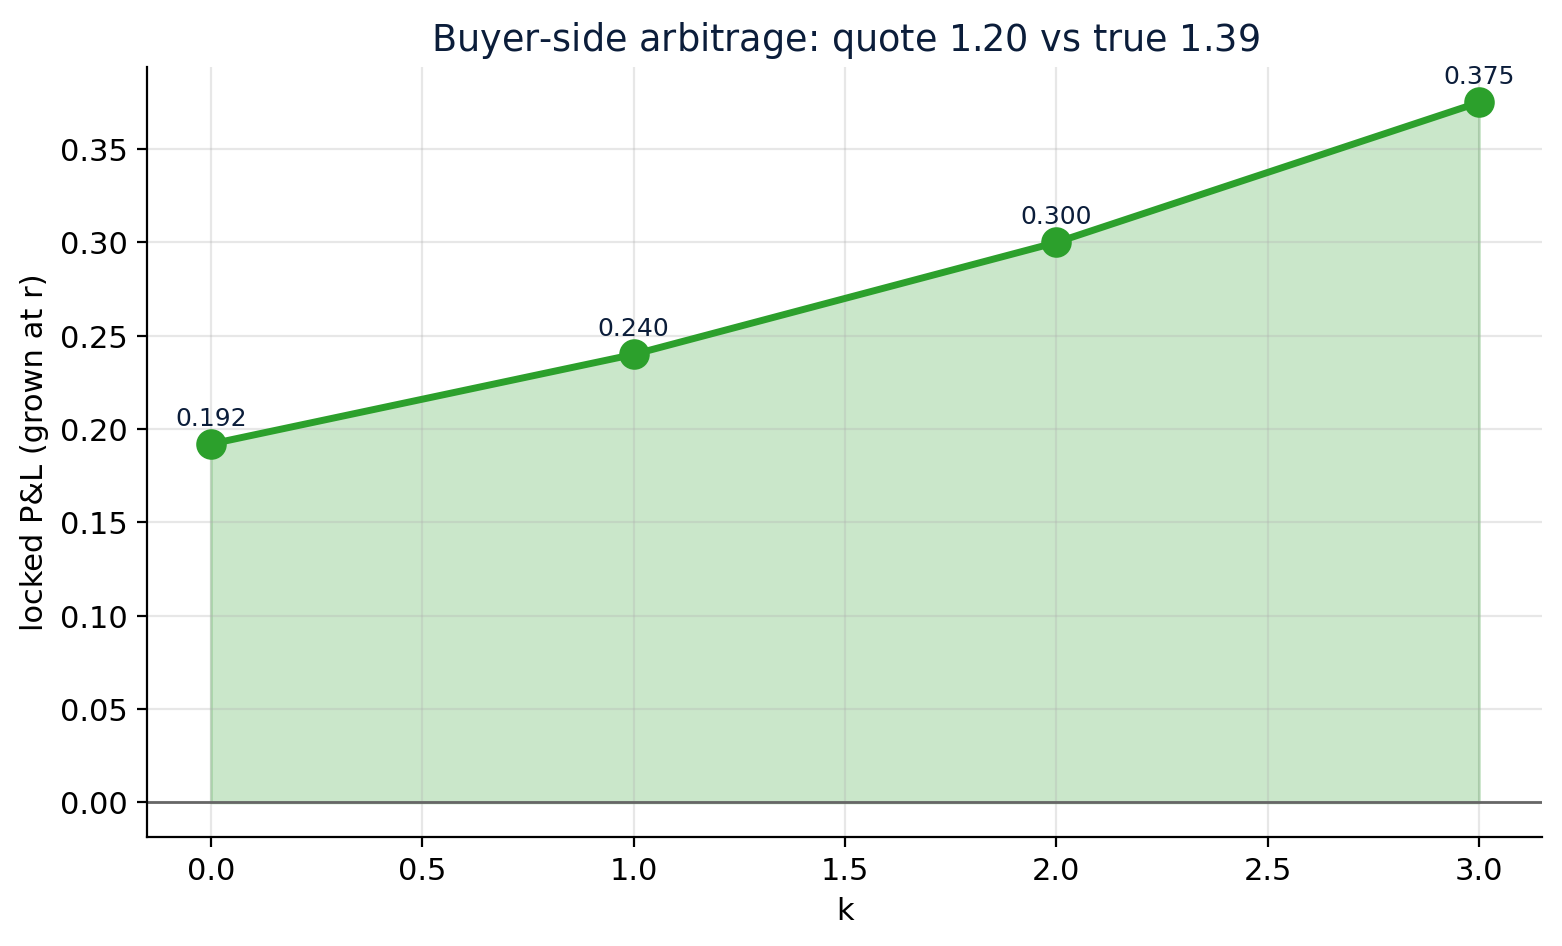
\includegraphics[keepaspectratio]{figures/ch04-arb-pnl.png}}
\caption{P\&L tree for the buyer-side arbitrage: ST put quoted at
\(1.20\) vs true \(1.36\). The locked-in \(0.16\) grows at \(r\) over
time.}
\end{figure}

\subsection{4.10.4 Table}\label{table-20}

\textbf{Table 4.15.} Buyer-side arbitrage P\&L on ST put \(K=5\) at
various mispricings:

{\def\LTcaptype{none} % do not increment counter
\begin{table}[H]
\centering
\begin{tabular}{|c|r|r|}
\toprule
quoted \(P\) & \(V_0 - P\) & locked-in \\
\midrule



\(1.00\) & \(\phantom{-}0.36\) & \(0.36\) \\
\(1.10\) & \(\phantom{-}0.26\) & \(0.26\) \\
\(1.20\) & \(\phantom{-}0.16\) & \(0.16\) \\
\(1.36\) & \(\phantom{-}0.00\) & fair \\
\(1.50\) & \(-0.14\) & \(0.14\) \\
\bottomrule
\end{tabular}
\end{table}
}

At \(P = 1.50\) the locked-in arb is on the dealer side (sell the put,
hedge cheaply).

\emph{Legend.} ``Fair'' = no arbitrage. Dealer-side: buyer is
over-paying, so the dealer captures the surplus.*

\begin{center}\rule{0.5\linewidth}{0.5pt}\end{center}

\section{§4.11 Path-dependence preview}\label{path-dependence-preview}

\textbf{Punchline.} For path-dependent contracts (knockouts, lookbacks,
Asians), the \emph{same} \((k, S_k)\) on different paths can have
\emph{different} option values, because the \emph{history} matters. To
price them, we \textbf{augment the state} with the relevant
path-statistic, breaking the recombining tree. Chapter 5's
reflection-based machinery will recover compactness.

\textbf{Intuition.} The recombining tree of Chapter 2 worked because the
European option payoff depended only on \(S_n\), and \(S_n\) depends
only on the \emph{number} of up moves, not their order. American payoffs
of standard puts/calls inherit this property --- the Snell value \(V_k\)
is a function of \((k, S_k)\) alone, so the tree still recombines. But
the moment the payoff depends on the path itself (did we touch \(B\)?
what is \(\min_{j \le k} S_j\)? what is
\(\frac{1}{k}\sum_{j \le k} S_j\)?), the value \(V_k\) must carry the
history. Two nodes at the same \((k, S_k)\) are no longer equivalent.

\subsection{\texorpdfstring{4.11.1 Knockout American --- same
\((k, S)\), different
fates}{4.11.1 Knockout American --- same (k, S), different fates}}\label{knockout-american-same-k-s-different-fates}

\textbf{Example 4.11.1 (ST n=3 knockout, \(K = 5, B = 8\)).} Consider
paths arriving at \((2, S = 4)\) from different histories:

\begin{itemize}
\tightlist
\item
  Path HT: \(S_0 = 4 \to S_1 = 8 \to S_2 = 4\). \textbf{Touched \(B\)}.
\item
  Path TH: \(S_0 = 4 \to S_1 = 2 \to S_2 = 4\). \textbf{Did not touch
  \(B\)}.
\end{itemize}

Both arrive at \((k=2, S=4)\). But: - On path HT, the option is
\textbf{knocked out}. \(V = 0\). - On path TH, the option is
\textbf{alive}. \(V = g(4) = 1\).

Same \((k, S)\), different \(V\). The augmented state is
\((k, S_k, \mathbf{1}_{\text{touched}})\).

\subsection{4.11.2 Augmented state space}\label{augmented-state-space}

\textbf{Example 4.11.2 (augmented state-space size).} For a recombining
\(n\)-step binomial tree with no path-dependence, the number of distinct
\((k, S_k)\) states is \(\binom{n+2}{2} \approx n^2/2\) --- polynomial
in \(n\).

For a knockout (one additional binary flag), the state space doubles
roughly: \(\approx n^2\). Still polynomial.

For a \emph{lookback} American with payoff \(g_k = (M_k - K)^+\) where
\(M_k = \max_{j \le k} S_j\), the state is \((k, S_k, M_k)\). The number
of distinct \((S_k, M_k)\) pairs is \(O(n^2)\) at each step, so total
state space is \(O(n^3)\).

For an \emph{Asian} American with \(g_k = (\bar S_k - K)^+\) where
\(\bar S_k = \frac{1}{k+1}\sum_{j=0}^k S_j\), the average \(\bar S_k\)
depends on the \emph{order} of up/down moves: there are up to \(2^k\)
distinct \(\bar S_k\) values. State space is \emph{exponential} in \(n\)
--- pricing requires either dimension-reduction tricks or Monte Carlo.

\textbf{Table:}

{\def\LTcaptype{none} % do not increment counter
\begin{table}[H]
\centering
\begin{tabular}{|l|l|c|}
\toprule
contract & augmented state & size \\
\midrule



Vanilla & \((k, S_k)\) & \(O(n^2)\) \\
Knockout & \((k, S_k, \mathbf{1}_{\text{hit}})\) & \(O(n^2)\) \\
Lookback (max) & \((k, S_k, M_k)\) & \(O(n^3)\) \\
Asian & \((k, S_k, \bar S_k)\) & \(O(2^n)\) \\
\bottomrule
\end{tabular}
\end{table}
}

\emph{All contracts are American (early-exercise) style.} ``Size'' is
the state-space size up to step \(n\).

\subsection{4.11.3 Lookback American}\label{lookback-american}

\textbf{Example 4.11.3 (ST American lookback put,
\(K - \min_{j} S_j\)).} Payoff at exercise time \(\tau\):
\(K - \min_{j \le \tau} S_j\). Take \(K = 4\).

For each of the 4 paths in the toy lattice we need to track the running
minimum:

{\def\LTcaptype{none} % do not increment counter
\begin{table}[H]
\centering
\begin{tabular}{|l|l|l|}
\toprule
path & \(S\) sequence & running min \(M_k\) \\
\midrule



HH & \(4, 8, 16\) & \(4, 4, 4\) \\
HT & \(4, 8, 4\) & \(4, 4, 4\) \\
TH & \(4, 2, 4\) & \(4, 2, 2\) \\
TT & \(4, 2, 1\) & \(4, 2, 1\) \\
\bottomrule
\end{tabular}
\end{table}
}

Intrinsic \(g_k = K - M_k\):

{\def\LTcaptype{none} % do not increment counter
\begin{table}[H]
\centering
\begin{tabular}{|l|r|r|r|}
\toprule
path & \(g_0\) & \(g_1\) & \(g_2\) \\
\midrule



HH & \(0\) & \(0\) & \(0\) \\
HT & \(0\) & \(0\) & \(0\) \\
TH & \(0\) & \(2\) & \(2\) \\
TT & \(0\) & \(2\) & \(3\) \\
\bottomrule
\end{tabular}
\end{table}
}

The state at \(k=1\): \((S_1, M_1)\). At \(S_1 = 8\), \(M_1 = 4\)
always. At \(S_1 = 2\), \(M_1 = 2\). So two distinct states at
\(k = 1\).

At \(k = 2\): at \(S_2 = 4\) via HT-path, \(M_2 = 4\); at \(S_2 = 4\)
via TH-path, \(M_2 = 2\). Two distinct states at the same \((k, S)\),
distinguished by \(M\).

Snell envelope must be indexed by \((k, S_k, M_k)\) here. Backward
induction is straightforward but the state-space has tripled.

\subsection{4.11.4 Reflection ahoy}\label{reflection-ahoy}

The Chapter 5 problem is: how to \emph{count} paths from \((0, 0)\) to
\((n, j)\) that touch a level \(L\)? The reflection principle of §0.7
will give a closed-form count, which is exactly what we need to price
barrier-style path-dependent contracts efficiently.

\textbf{Example 4.11.4 (reflection preview).} Count paths from
\((0, 0)\) to \((4, 2)\) that touch level \(3\) (in ``net up-count''
coordinates). By the reflection bijection of §0.7: such paths are in 1-1
correspondence with paths from \((0, 0)\) to \((4, 2L - 2) = (4, 4)\).
There are \(\binom{4}{4} = 1\) such path (UUUU). So exactly \textbf{1
path} of length 4 ends at level \(+2\) and touches level \(3\).

That's exactly the count needed to price an up-and-out barrier:
``fraction of paths surviving to the endpoint'' = total paths minus
barrier-touchers.

In Chapter 5 this counting machinery extends to lookback options, Asian
options, and exotic barriers --- turning path-dependence from a
state-space-explosion problem back into a tractable closed form.

\begin{figure}
\centering
\pandocbounded{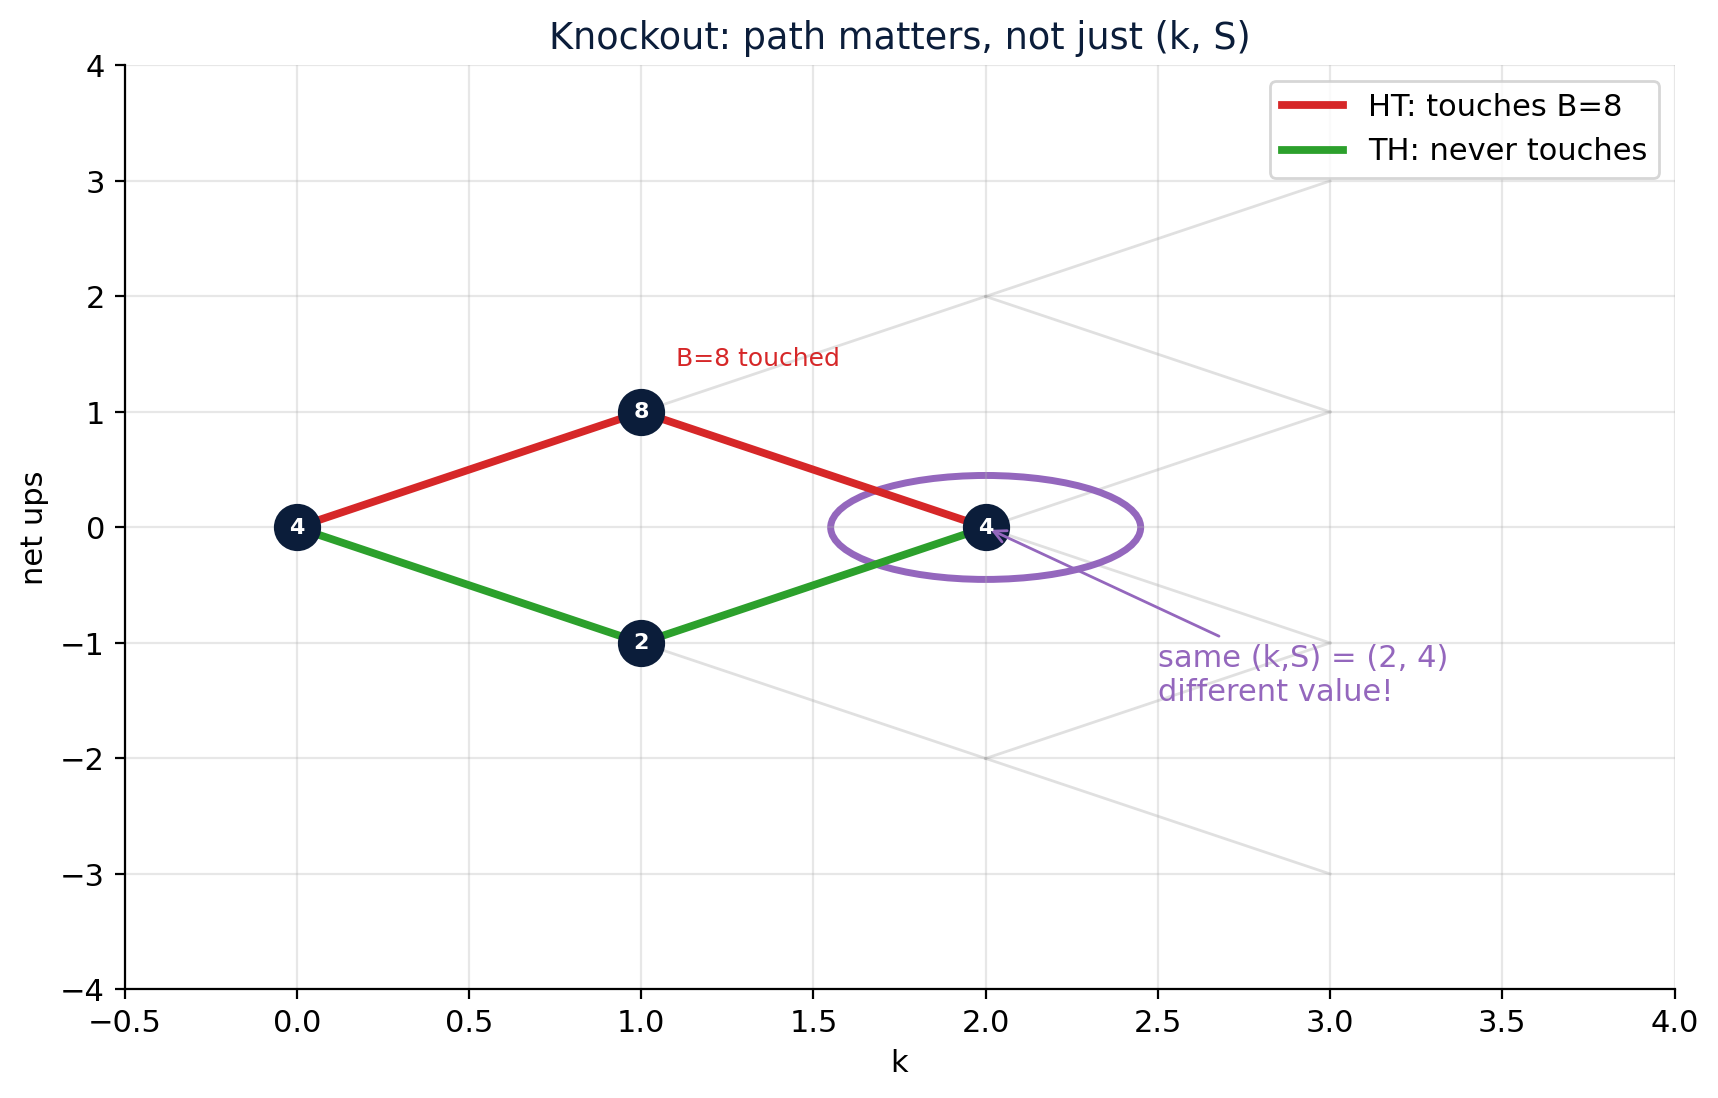
\includegraphics[keepaspectratio]{figures/ch04-knockout-same-S.png}}
\caption{ST knockout: two paths arriving at the same \((k, S) = (2, 4)\)
--- but path HT touched \(B = 8\) and is knocked out, while path TH
never touched and is alive. Same \((k, S)\), different option values.}
\end{figure}

\begin{figure}
\centering
\pandocbounded{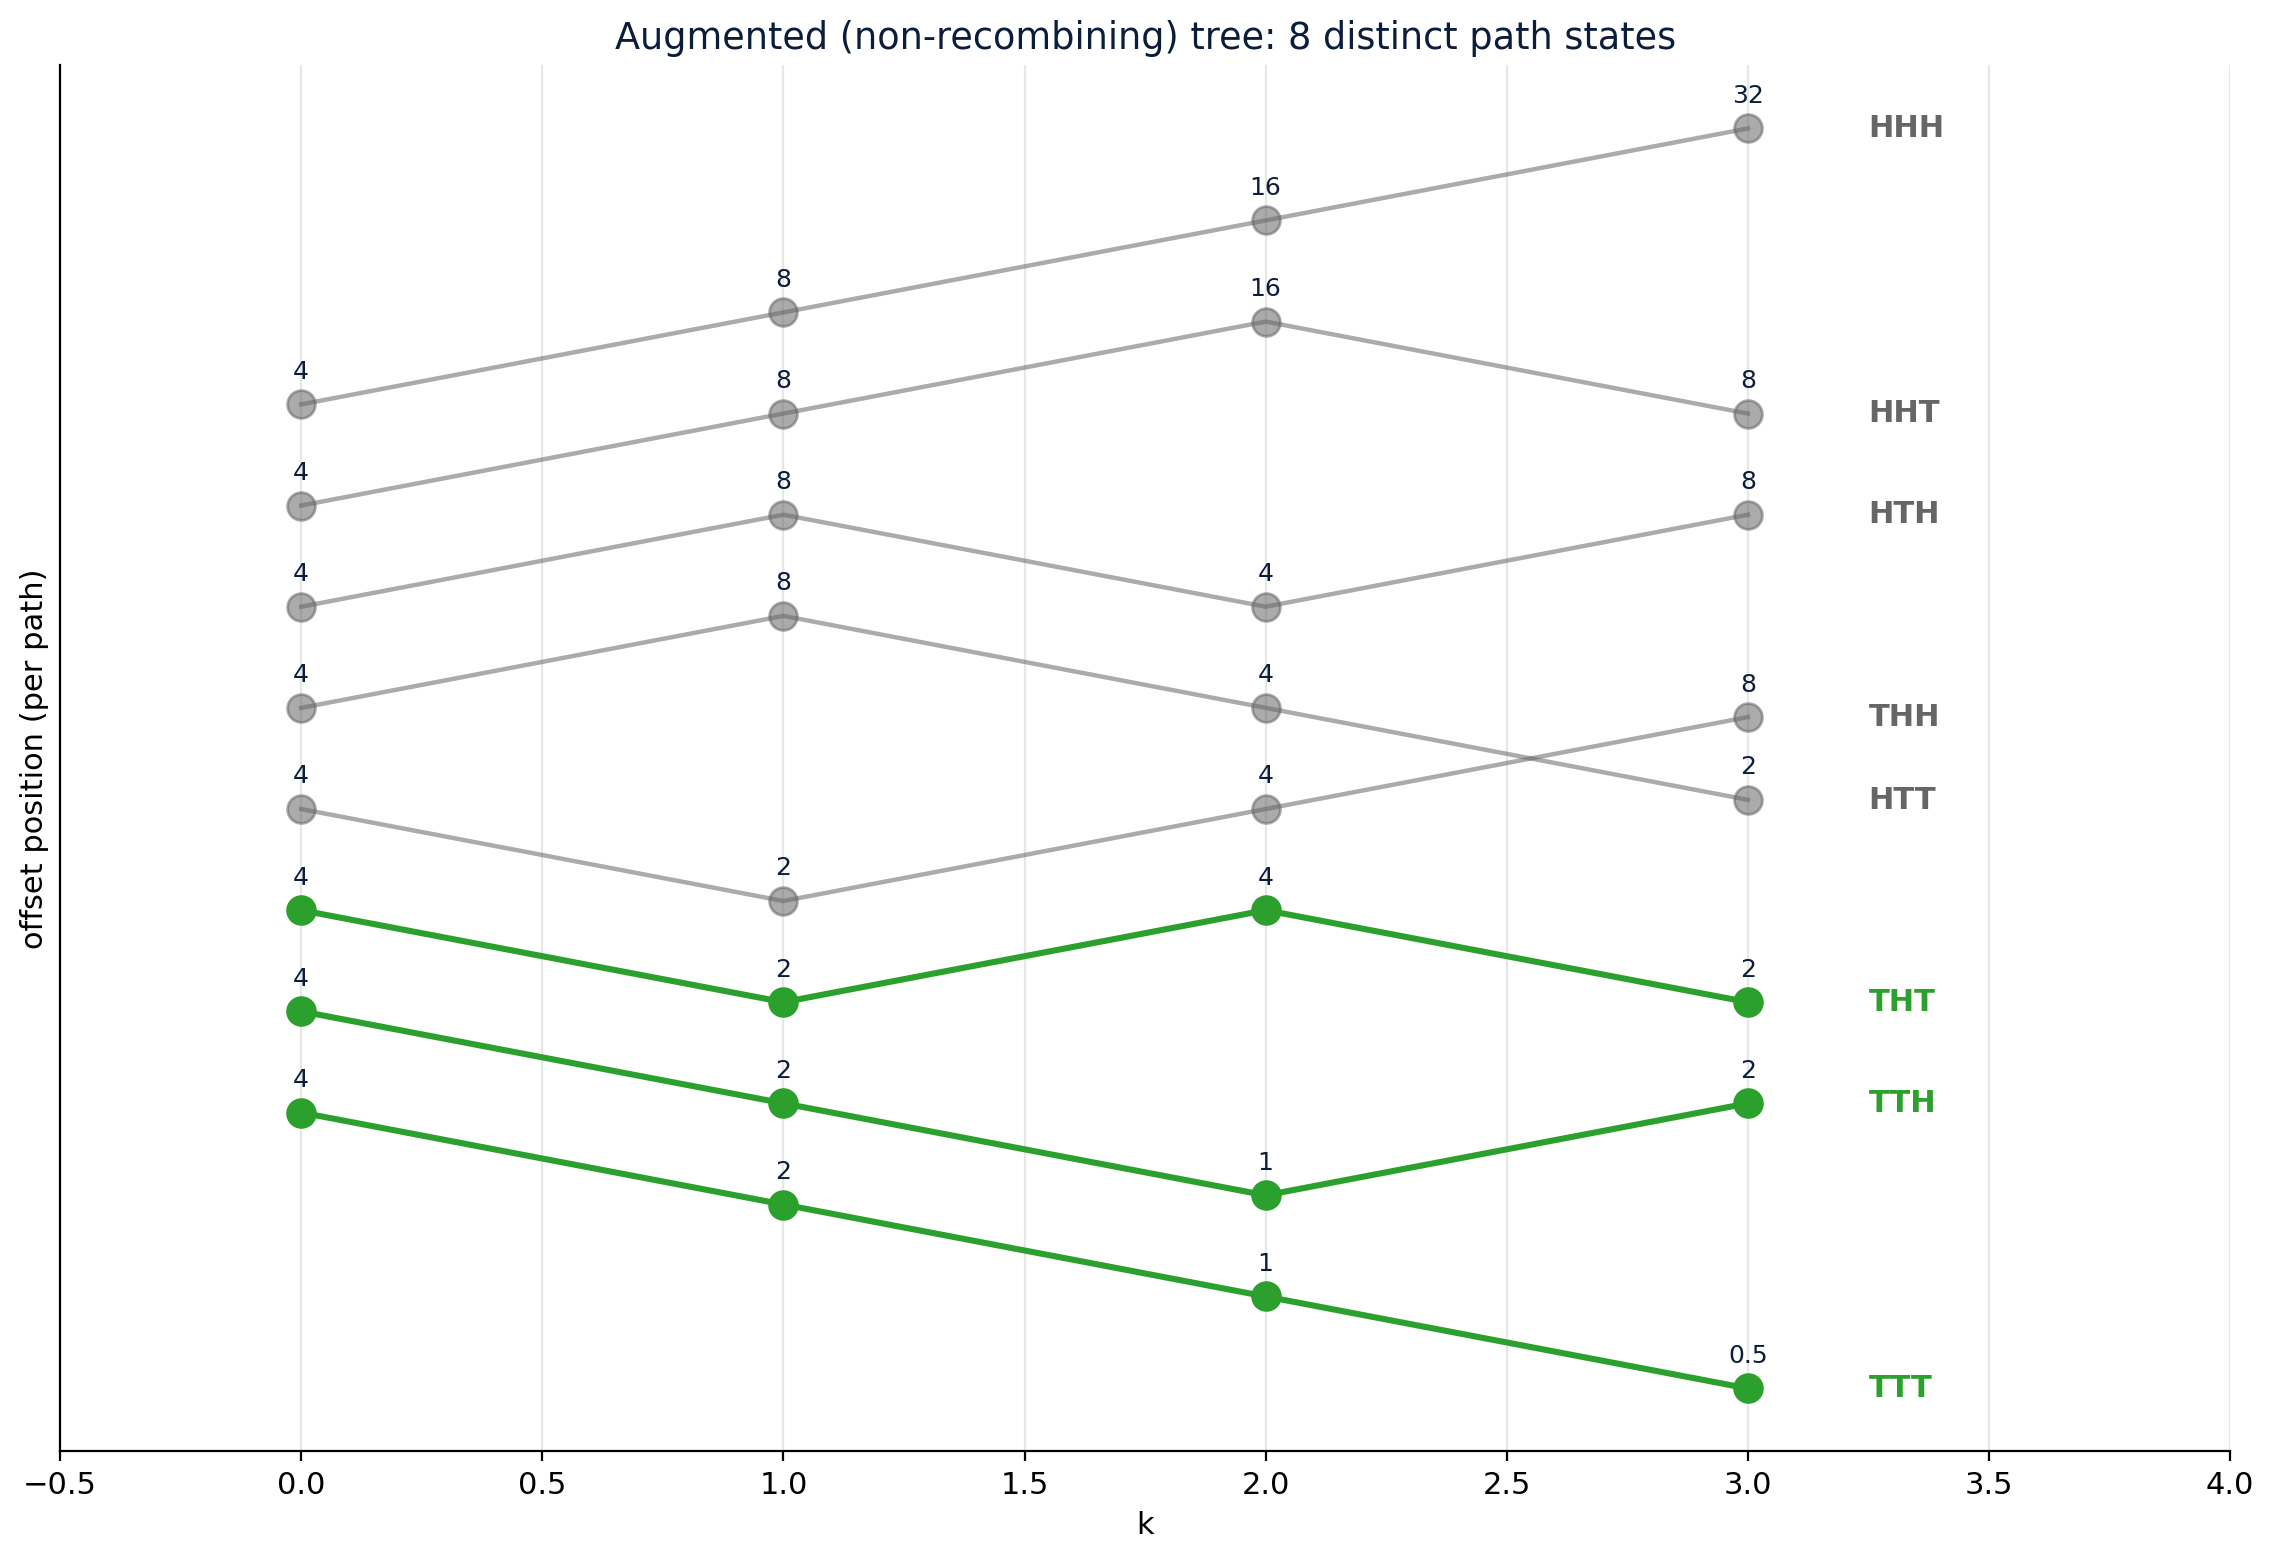
\includegraphics[keepaspectratio]{figures/ch04-augmented-tree.png}}
\caption{Augmented (non-recombining) tree for \(n = 3\) knockout: each
of the 8 paths is a distinct state once the barrier-touched flag is
included. Grey paths are knocked out.}
\end{figure}

\subsection{4.11.5 Table}\label{table-21}

\textbf{Table 4.16.} State-space size for path-dependent American
contracts.

(Reproduced from §4.11.2.)

\begin{center}\rule{0.5\linewidth}{0.5pt}\end{center}

\section{Chapter summary}\label{chapter-summary-1}

The American buyer chooses an optimal stopping time \(\tau^*\) to
maximise expected discounted payoff under \(\tilde{\mathbb{P}}\). The
value function \(V_k\) (the Snell envelope) is computed by backward
induction:

\[V_n = g(S_n), \qquad V_k = \max\{g(S_k),\, \beta\tilde{\mathbb{E}}[V_{k+1}\mid\mathcal F_k]\}.\]

The optimal stopping time is the first time \(V_k\) touches the
intrinsic \(g(S_k)\). The continuation region is downward-closed for a
put on a non-dividend stock; the exercise frontier moves up with \(r\),
down with \(\sigma\), and up with \(k\) as maturity approaches. For a
non-dividend call, early exercise is never optimal --- American \(=\)
European. Dealers hedge by super-replicating; consumption at
exercise-region nodes absorbs the supermartingale slack. Mispricings on
either side create textbook arbitrages.

We have priced exotics --- digitals, knockouts, choosers, range-accruals
--- by re-using the Snell recipe with custom payoffs. We have also seen
that \emph{path-dependence} breaks the recombining tree: barrier
options, lookbacks, and Asians require augmented state. That
augmentation is the bridge to Chapter 5.

\begin{center}\rule{0.5\linewidth}{0.5pt}\end{center}

\section{Bridge to Chapter 5}\label{bridge-to-chapter-5}

We've seen that the American exercise region depends on the
\textbf{path} as soon as the contract has any path-dependence
(knockouts, lookbacks, Asians). Two nodes at the same \((k, S_k)\) may
carry completely different option values because their \emph{histories}
--- barrier-touched, running maximum, running average --- differ. The
augmented state space can balloon, in the Asian case to \(O(2^n)\).

To price path-dependent contracts efficiently --- barriers, lookbacks,
fixed-strike Asians, even American versions of these --- we need a way
to \textbf{count paths that hit certain levels} without enumerating each
one. The reflection principle from §0.7 is about to do real work: it
gives closed-form counts that turn an apparently exponential state space
back into a tractable polynomial computation.

Chapter 5 develops the path-counting toolkit: reflection in its full
form, the joint distribution of \((S_n, M_n)\) where \(M_n\) is the
running max, the \emph{first-passage} time distribution, and the
resulting closed forms for European and American barrier options. Once
we have those tools, lookbacks, Asians, and discrete barriers all yield
to the same machinery.

We turn now to that chapter.

\begin{center}\rule{0.5\linewidth}{0.5pt}\end{center}

\newpage

\chapter{Chapter 5 --- The Random Walk and the Reflection
Principle}\label{chapter-5-the-random-walk-and-the-reflection-principle}

\section{How to read this chapter}\label{how-to-read-this-chapter-4}

In Chapter 2 we toured the multi-period binomial tree and the
Fundamental Theorem of Asset Pricing. In Chapter 3 we put stopping times
and martingales onto that tree. In Chapter 4 we discovered that some
payoffs --- barriers, lookbacks, Asians, Americans --- depend on the
\emph{whole path}, not just the endpoint.

A path-dependent payoff is the engineer's nightmare. To price it
naively, you sum over \(2^n\) paths. At \(n = 20\) that is a million
paths; at \(n = 30\) it is a billion. We cannot sustain this for any
practical model.

\textbf{This chapter is the rescue.} A symmetric random walk has a
hidden symmetry --- \emph{reflection} --- that converts path-dependent
path counts into endpoint counts. We will:

\begin{enumerate}
\def\labelenumi{\arabic{enumi}.}
\tightlist
\item
  Look at the random walk \(X_n\) that lives inside every binomial tree
  (§5.1).
\item
  Track its running maximum \(M_n\) --- the object that detects barriers
  and lookbacks (§5.2).
\item
  Build the \textbf{reflection principle} very slowly from tiny
  enumerations (§5.3) --- this is the heart of the chapter and the part
  that previous drafts skipped over too quickly.
\item
  Read first-passage time distributions off the reflection principle
  (§5.4).
\item
  Get the joint distribution of \((M_n, X_n)\) in one short formula
  (§5.5).
\item
  Price knock-in / knock-out barrier options on the binomial tree
  (§5.6).
\item
  Price lookback options (§5.7).
\item
  Connect the picture to American options (§5.8).
\item
  Watch reflection survive the \(n \to \infty\) limit and reproduce
  Black-Scholes barriers (§5.9, §5.10).
\end{enumerate}

\textbf{The mantra.} \emph{Reflection is a counting argument.} It does
not require calculus, measure theory, or Itô. It works on a piece of
paper because the random walk is a collection of integer lattice paths,
and lattice paths can be reflected across horizontal lines. The fact
that the same identity will survive the continuous-time limit is a happy
bonus that we will witness empirically in §5.9.

What we still avoid in this chapter: derivatives, integrals,
\(\sigma\)-algebras as abstract objects. Every ``expectation'' is a
finite sum, every ``probability'' is a count over \(2^n\).

\begin{center}\rule{0.5\linewidth}{0.5pt}\end{center}

\section{§5.1 The Symmetric Random
Walk}\label{the-symmetric-random-walk}

\textbf{Punchline.} A fair coin tossed \(n\) times traces a polygonal
path on the integer lattice, going up by one on a head and down by one
on a tail. That path \emph{is} a log-stock-price in disguise.

\textbf{Intuition.} Forget options for a moment. Imagine you stand on
the integer number line at position \(0\) at time \(0\). Every second
you flip a fair coin: heads you take one step right, tails one step
left. Your position after \(n\) flips is a random integer. Watch the
\emph{whole trajectory} of your position over time and you have what
statisticians call a \emph{symmetric simple random walk}. It is the
simplest non-trivial stochastic process. Everything in this chapter ---
and a lot of what comes after --- is a statement about this walk.

Why care? Because in a binomial tree with \(\log u = -\log d = \sigma\),
the log-price increment is exactly \(\sigma \cdot (\pm 1)\). The
log-price \emph{is} the random walk, scaled.

\subsection{5.1.1 Definitions}\label{definitions-15}

Let \(\xi_1, \xi_2, \ldots, \xi_n\) be independent random variables,
each taking value \(+1\) or \(-1\) with probability \(\tfrac12\). Define

\[X_0 = 0, \qquad X_n = \xi_1 + \xi_2 + \cdots + \xi_n.\]

We call \(X_n\) the \textbf{symmetric simple random walk} after \(n\)
steps. The sequence \(\{X_0, X_1, \ldots, X_n\}\) is the \textbf{path}
of the walk.

Three immediate facts.

\textbf{Fact 1 (parity).} \(X_n\) has the same parity as \(n\): if \(n\)
is even then \(X_n\) is even, and if \(n\) is odd then \(X_n\) is odd.
In particular \(X_n \in \{-n, -n+2, -n+4, \ldots, n-2, n\}\), a set of
\(n+1\) integers.

\textbf{Fact 2 (distribution).} The number of paths reaching \(X_n = k\)
is the number of ways to pick which of the \(n\) steps were \(+1\). If
\(X_n = k\) then the number of \(+1\) steps is \((n+k)/2\). Hence

\[\boxed{\;\mathbb P(X_n = k) \;=\; \frac{1}{2^n}\binom{n}{\tfrac{n+k}{2}}\;}\]

for integers \(k\) of the same parity as \(n\), and \(0\) otherwise.

\textbf{Fact 3 (moments).} \(\mathbb E[\xi_i] = 0\),
\(\mathrm{Var}(\xi_i) = 1\), so by independence

\[\mathbb E[X_n] = 0, \qquad \mathrm{Var}(X_n) = n.\]

The standard deviation grows like \(\sqrt n\) --- slower than \(n\). We
will meet this fact repeatedly.

\subsection{\texorpdfstring{5.1.2 The stock-price connection (
\(u = 2\),
\(d = 1/2\))}{5.1.2 The stock-price connection ( u = 2, d = 1/2)}}\label{the-stock-price-connection-u-2-d-12}

Our running Toy example uses \(S_0 = 4\), \(u = 2\), \(d = 1/2\),
\(r = 1/4\) (the same Toy as Chapter 2). With
\(\log u = -\log d = \log 2\), the log-stock-price increment per step is
\(\pm \log 2\). Hence

\[\log(S_n / S_0) \;=\; X_n \cdot \log 2 \qquad \Longleftrightarrow \qquad S_n \;=\; S_0 \cdot 2^{X_n} \;=\; 4 \cdot 2^{X_n}.\]

This is a one-to-one correspondence. Every fact we prove about \(X_n\)
translates to a fact about \(S_n\) --- we just exponentiate.

In the more realistic case \(u = 1.10\), \(d = 0.90\), we have
\(\log u \approx 0.0953\) and \(\log d \approx -0.1054\). The two
magnitudes are slightly unequal, so the log walk is \emph{not} perfectly
symmetric --- an up-step is a little smaller than a down-step in log
space. This asymmetry is small (\(\sim 5\%\) of the move size) and we
will keep working with the unequal log magnitudes for realistic
examples; the \emph{reflection principle} in §5.3 assumes the symmetric
walk and applies cleanly only when \(\log u + \log d = 0\),
i.e.~\(ud = 1\). For the toy we have \(ud = 1\) exactly.

\textbf{Intuition (when does reflection work?).} Reflection assumes the
walk is \emph{symmetric}: an up-step and a down-step have the same size.
In the toy (\(ud = 1\)) the log walk is perfectly symmetric. In
realistic models (\(ud \ne 1\)) it is not, but we can still price by
direct enumeration --- and as \(n\) grows large with \(u, d\) chosen so
that \(\log u, |\log d|\) are both \(O(1/\sqrt n)\), the asymmetry
shrinks and reflection becomes asymptotically exact (the Black-Scholes
limit, §5.10).

\subsection{5.1.3 Examples}\label{examples-23}

\textbf{Example 5.1.1 (all eight length-3 paths).} With \(n = 3\) there
are \(2^3 = 8\) paths. Each is encoded by a string of three letters from
\(\{U, D\}\). We compute the running position \(X_n\):

{\def\LTcaptype{none} % do not increment counter
\begin{table}[H]
\centering
\begin{tabular}{|l|r|r|r|r|}
\toprule
Path & \(X_0\) & \(X_1\) & \(X_2\) & \(X_3\) \\
\midrule



UUU & 0 & +1 & +2 & +3 \\
UUD & 0 & +1 & +2 & +1 \\
UDU & 0 & +1 & 0 & +1 \\
UDD & 0 & +1 & 0 & \(-1\) \\
DUU & 0 & \(-1\) & 0 & +1 \\
DUD & 0 & \(-1\) & 0 & \(-1\) \\
DDU & 0 & \(-1\) & \(-2\) & \(-1\) \\
DDD & 0 & \(-1\) & \(-2\) & \(-3\) \\
\bottomrule
\end{tabular}
\end{table}
}

Tabulating the terminal values:

{\def\LTcaptype{none} % do not increment counter
\begin{table}[H]
\centering
\begin{tabular}{|r|r|r|r|r|}
\toprule
\(k\) & \(-3\) & \(-1\) & \(+1\) & \(+3\) \\
\midrule



paths to \(X_3 = k\) & \(1\) (DDD) & \(3\) (DDU, DUD, UDD) & \(3\) (DUU,
UDU, UUD) & \(1\) (UUU) \\
\(\mathbb P(X_3 = k)\) & \(1/8\) & \(3/8\) & \(3/8\) & \(1/8\) \\
\bottomrule
\end{tabular}
\end{table}
}

The row of counts is Pascal's triangle row \(n = 3\): \(1, 3, 3, 1\).
The formula \(\binom{3}{(3+k)/2}/8\) gives the same thing.

\textbf{Example 5.1.2 (\(\mathbb P(X_4 = 2)\)).} Two ways:

\emph{Formula:}
\(\binom{4}{(4+2)/2}/2^4 = \binom{4}{3}/16 = 4/16 = 1/4\).

\emph{Enumeration:} paths of length 4 with exactly three U's: UUUD,
UUDU, UDUU, DUUU --- four paths. So \(\mathbb P(X_4 = 2) = 4/16 = 1/4\).
✓

\textbf{Example 5.1.3 ( \(n=3\) stock paths from \(S_0 = 4\)).} With
\(S_n = 4 \cdot 2^{X_n}\):

{\def\LTcaptype{none} % do not increment counter
\begin{table}[H]
\centering
\begin{tabular}{|l|r|r|}
\toprule
Path & \(X_3\) & \(S_3\) \\
\midrule



UUU & \(+3\) & \(32\) \\
UUD & \(+1\) & \(8\) \\
UDU & \(+1\) & \(8\) \\
UDD & \(-1\) & \(2\) \\
DUU & \(+1\) & \(8\) \\
DUD & \(-1\) & \(2\) \\
DDU & \(-1\) & \(2\) \\
DDD & \(-3\) & \(0.5\) \\
\bottomrule
\end{tabular}
\end{table}
}

The eight terminal stock prices are \(\{32, 8, 8, 2, 8, 2, 2, 0.5\}\)
--- the multiplicities are \(1, 3, 3, 1\), the same Pascal row. The tree
is recombining: only the \emph{count} of U's matters for \(S_n\), not
the order.

\textbf{Example 5.1.4 (realistic, \(u=1.10\), \(d=0.90\), \(n=3\)).} Now
\(S_n = 100 \cdot 1.10^{n_U} \cdot 0.90^{n - n_U}\). Enumerated:

{\def\LTcaptype{none} % do not increment counter
\begin{table}[H]
\centering
\begin{tabular}{|l|r|r|}
\toprule
Path & \(n_U\) & \(S_3\) \\
\midrule



UUU & 3 & \(133.10\) \\
UUD & 2 & \(108.90\) \\
UDU & 2 & \(108.90\) \\
UDD & 1 & \(89.10\) \\
DUU & 2 & \(108.90\) \\
DUD & 1 & \(89.10\) \\
DDU & 1 & \(89.10\) \\
DDD & 0 & \(72.90\) \\
\bottomrule
\end{tabular}
\end{table}
}

The log-prices are
\(\log(S_n/100) \in \{0.286, 0.085, \ldots, -0.314\}\). Note
\(|0.286 / 3 - (-0.314)/3| > 0\) --- so up- and down-log-moves differ in
magnitude by about \(5\%\). The log walk is \emph{not} perfectly
symmetric, although it is very close.

\textbf{Example 5.1.5 (mean and variance).} Take \(n = 100\).
\(\mathbb E[X_{100}] = 0\), \(\mathrm{Var}(X_{100}) = 100\), so
\(\mathrm{sd}(X_{100}) = 10\). A random length-100 walk typically ends
within \(\pm 10\) of zero, and almost never further than \(\pm 30\).

\textbf{Example 5.1.6 (\(\mathbb P(X_4 \ge 0)\)).} Five values
\(k \in \{-4, -2, 0, 2, 4\}\). Counts \(1, 4, 6, 4, 1\) from row 4 of
Pascal. Then

\[\mathbb P(X_4 \ge 0) \;=\; \frac{6 + 4 + 1}{16} \;=\; \frac{11}{16} \;=\; 0.6875.\]

By enumeration: out of 16 paths of length 4, eleven end at
\(X_4 \in \{0, 2, 4\}\). Cross-checked.

\textbf{Example 5.1.7 (\(\mathbb P(X_4 \ge 2)\)).}
\(\binom{4}{3}/16 + \binom{4}{4}/16 = 4/16 + 1/16 = 5/16\).

\textbf{Example 5.1.8 (a back-of-envelope rare-event estimate).} For
\(n = 100\) steps and target level \(k = 30\):
\(\mathrm{sd}(X_{100}) = 10\), so \(X_{100} = 30\) is ``three sigma.''
The CLT (Chapter 0) says the chance is about \(0.0013\). Cross-checking
with the exact formula,
\(\mathbb P(X_{100} = 30) = \binom{100}{65}/2^{100}\), which is roughly
\(0.00075\). The continuous approximation is in the right ballpark.

\textbf{Example 5.1.9 (a paradox of symmetry).} Suppose the walk has
gone up 10 times in a row. Is it more likely to come down next?
\emph{No.} The fair coin has no memory:
\(\mathbb P(\xi_{11} = +1) = 1/2\) regardless of the previous ten flips.
The walker's \emph{running position} will probably come down on average
(regression to zero), but each individual step is fair.

\begin{figure}
\centering
\pandocbounded{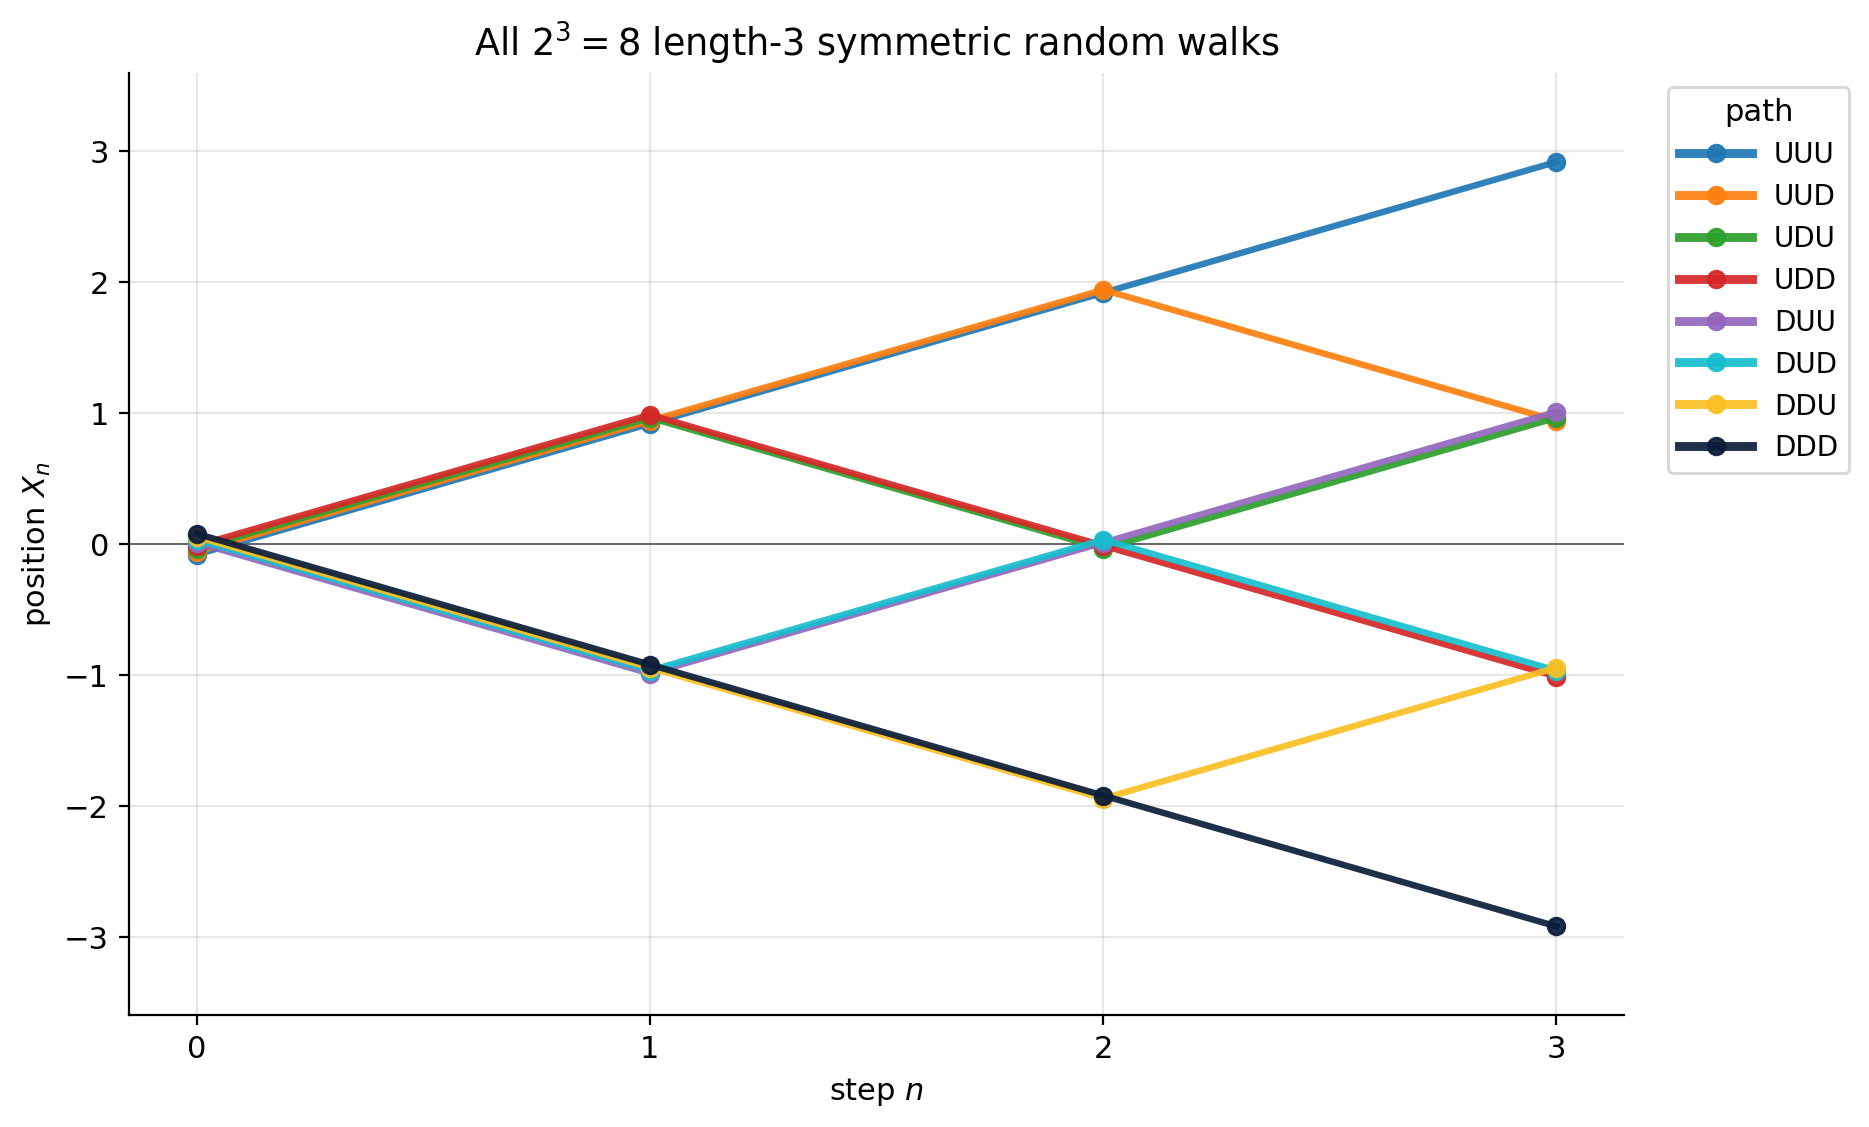
\includegraphics[keepaspectratio]{figures/ch05-8-paths.png}}
\caption{All \(2^3 = 8\) length-3 paths of the symmetric random walk,
colour-coded. The four paths ending at \(+1\) overlap in their endpoint
but visit different sets of states in between; that ``visit'' is exactly
the information barrier and lookback options care about.}
\end{figure}

\begin{figure}
\centering
\pandocbounded{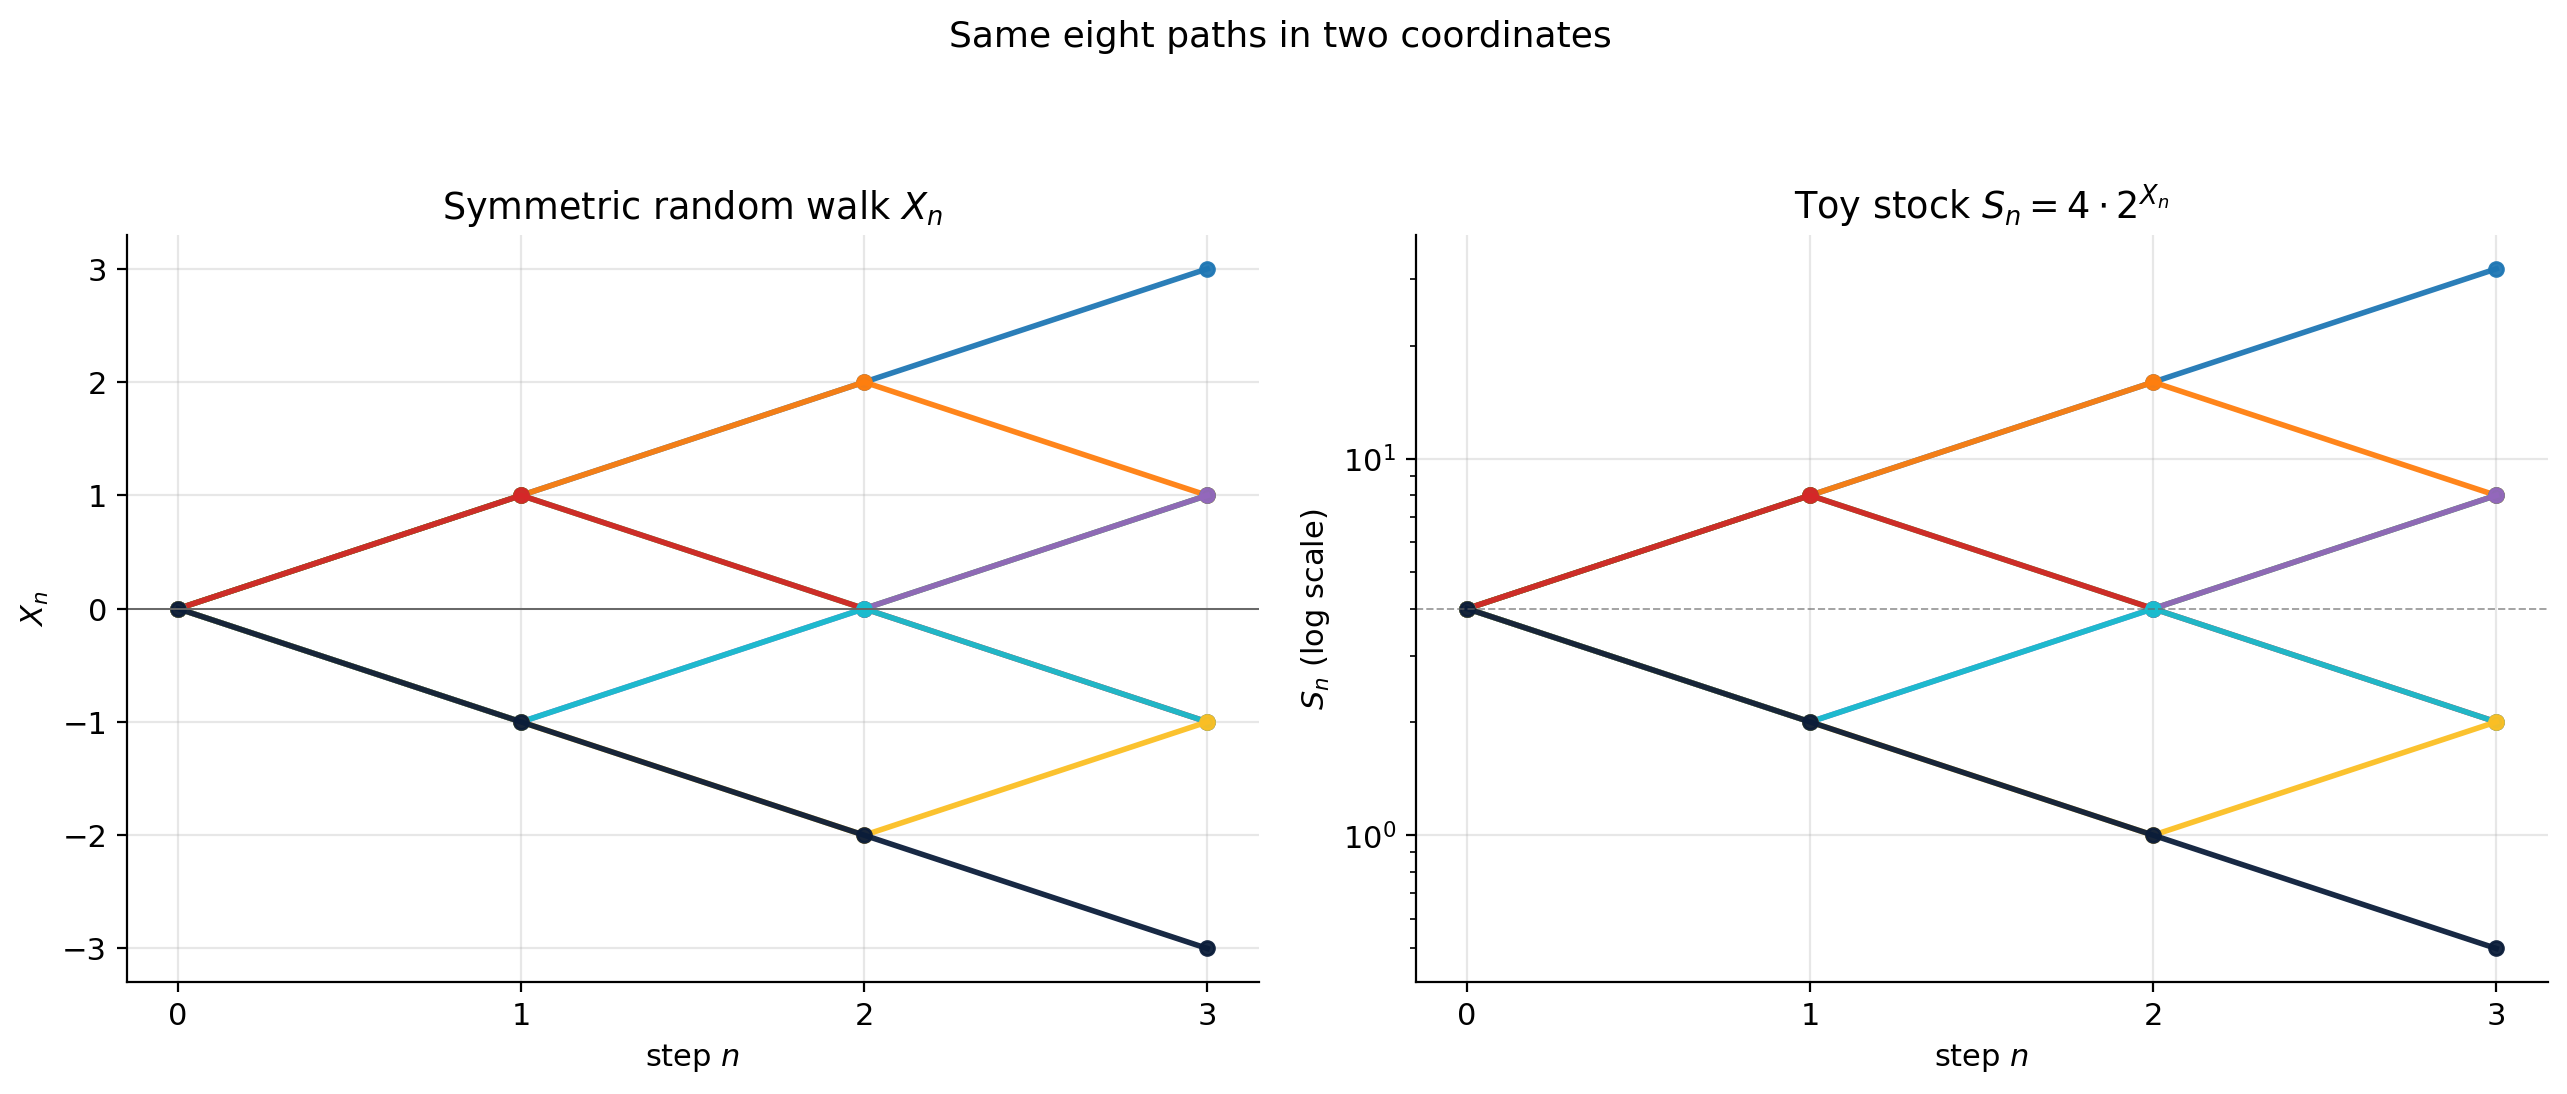
\includegraphics[keepaspectratio]{figures/ch05-paths-vs-stock.png}}
\caption{The same eight length-3 paths plotted as random walks \(X_n\)
(left) and as stock paths \(S_n = 4 \cdot 2^{X_n}\) on a log axis
(right). The two pictures are the same plot in different coordinates:
\(\log_2(S_n/4) = X_n\).}
\end{figure}

\subsection{5.1.4 Tables}\label{tables-11}

\textbf{Table 5.1.} Distribution of \(X_n\) for \(n = 1, 2, 3, 4, 5\).
Each row sums to \(2^n\) paths (and \(1.0\) in probability).

{\def\LTcaptype{none} % do not increment counter
\begin{table}[H]
\centering
\begin{tabular}{|r|r|r|r|r|r|r|r|r|r|r|r|}
\toprule
\(n\) & \(X_n = -5\) & \(-4\) & \(-3\) & \(-2\) & \(-1\) & \(0\) & \(+1\) & \(+2\) & \(+3\) & \(+4\) & \(+5\) \\
\midrule



\(1\) & & & & & \(\phantom{0}1\) & & \(\phantom{0}1\) & & & & \\
\(2\) & & & & \(\phantom{0}1\) & & \(\phantom{0}2\) & & \(\phantom{0}1\)
& & & \\
\(3\) & & & \(1\) & & \(\phantom{0}3\) & & \(\phantom{0}3\) & & \(1\) &
& \\
\(4\) & & \(1\) & & \(\phantom{0}4\) & & \(\phantom{0}6\) & &
\(\phantom{0}4\) & & \(1\) & \\
\(5\) & \(1\) & & \(5\) & & \(10\) & & \(10\) & & \(5\) & & \(1\) \\
\bottomrule
\end{tabular}
\end{table}
}

\emph{Blank: \(\mathbb P(X_n = k) = 0\) by parity (n and k must agree
mod 2).}

\textbf{Table 5.2.} Same data as probabilities (divide each row by
\(2^n\)).

{\def\LTcaptype{none} % do not increment counter
\begin{table}[H]
\centering
\begin{tabular}{|r|r|r|r|r|r|r|r|r|r|r|r|}
\toprule
\(n\) & \(-5\) & \(-4\) & \(-3\) & \(-2\) & \(-1\) & \(0\) & \(+1\) & \(+2\) & \(+3\) & \(+4\) & \(+5\) \\
\midrule



\(1\) & & & & & \(0.5000\) & & \(0.5000\) & & & & \\
\(2\) & & & & \(0.2500\) & & \(0.5000\) & & \(0.2500\) & & & \\
\(3\) & & & \(0.1250\) & & \(0.3750\) & & \(0.3750\) & & \(0.1250\) &
& \\
\(4\) & & \(0.0625\) & & \(0.2500\) & & \(0.3750\) & & \(0.2500\) & &
\(0.0625\) & \\
\(5\) & \(0.0313\) & & \(0.1563\) & & \(0.3125\) & & \(0.3125\) & &
\(0.1563\) & & \(0.0313\) \\
\bottomrule
\end{tabular}
\end{table}
}

\emph{Blank: \(\mathbb P(X_n = k) = 0\) by parity.}

\subsection{5.1.5 Exercises}\label{exercises-21}

\begin{enumerate}
\def\labelenumi{\arabic{enumi}.}
\tightlist
\item
  Compute \(\mathbb P(X_6 = 0)\). \textbf{Answer:}
  \(\binom{6}{3}/64 = 20/64 = 0.3125\).
\item
  Compute \(\mathbb P(X_{10} \ge 4)\) using only Table 5.1's pattern
  (Pascal row 10 is \(1, 10, 45, 120, 210, 252, 210, 120, 45, 10, 1\)).
  \textbf{Answer:} \((45 + 10 + 1)/1024 = 56/1024 \approx 0.0547\).
\item
  The stock with \(S_0 = 4\) reaches what set of values at time
  \(n = 4\)? \textbf{Answer:} \(\{64, 16, 4, 1, 0.25\}\) --- five
  values, with \(S_n = 4 \cdot 2^{X_4}\).
\end{enumerate}

\begin{center}\rule{0.5\linewidth}{0.5pt}\end{center}

\section{\texorpdfstring{§5.2 The Running Maximum
\(M_n\)}{§5.2 The Running Maximum M\_n}}\label{the-running-maximum-m_n}

\textbf{Punchline.} Barrier options ask ``did the path \emph{ever} touch
level \(L\)?'' That's the running maximum: \(M_n \ge L\). Lookback
options ask ``how high did it go?'' That's \(M_n\). The running max is
the single object that turns a \emph{path-history} question into a
\emph{path-statistic} question.

\textbf{Intuition.} Imagine watching the walker step by step and writing
down the largest position they have visited so far. That number cannot
decrease --- it can only stay the same or jump up. The graph of \(M_n\)
is a non-decreasing staircase that traces the upper envelope of the
path. If you ever care about a barrier or a peak, you really only care
about this staircase.

\subsection{5.2.1 Definitions}\label{definitions-16}

For the random walk \(X_0, X_1, \ldots, X_n\), define

\[M_n \;=\; \max_{0 \le k \le n} X_k.\]

Some immediate properties.

\begin{itemize}
\tightlist
\item
  \(M_n \ge X_0 = 0\) always. So \(M_n\) is a non-negative integer.
\item
  \(M_n \ge X_n\) always (the running max is at least the final
  position).
\item
  \(M_n\) is non-decreasing: \(M_{n+1} \ge M_n\).
\item
  \(M_n - X_n \ge 0\) is the \textbf{drawdown from peak}, the amount by
  which the walk has retreated from its maximum.
\end{itemize}

\textbf{Stock-price barrier translation.} If
\(S_n = S_0 \cdot u^{n_U} d^{n_D}\) with \(u = 2\), \(d = 1/2\), the
barrier ``\(S\) ever reaches 16 starting from \(S_0 = 4\)'' is the same
as ``\(X\) ever reaches \(\log_2(16/4) = 2\)'' --- i.e.~\(M_n \ge 2\).
\textbf{A barrier on \(S\) is a barrier on \(X\).}

In general for \(\log u = -\log d = \sigma\):

\[M^S_n \;=\; \max_{0 \le k \le n} S_k \;=\; S_0 \cdot u^{M_n}.\]

So \(M^S_n \ge L\) iff \(M_n \ge \log_u(L/S_0)\). We solve for the
\(X\)-level \(m\) then count.

\subsection{5.2.2 Examples}\label{examples-24}

\textbf{Example 5.2.1 (all eight length-3 paths with \((X_3, M_3)\)).}
Add the running max column to the table from Example 5.1.1:

{\def\LTcaptype{none} % do not increment counter
\begin{table}[H]
\centering
\begin{tabular}{|l|r|r|r|r|}
\toprule
Path & \(X_1\) & \(X_2\) & \(X_3\) & \(M_3\) \\
\midrule



UUU & \(+1\) & \(+2\) & \(+3\) & \(3\) \\
UUD & \(+1\) & \(+2\) & \(+1\) & \(2\) \\
UDU & \(+1\) & \(0\) & \(+1\) & \(1\) \\
UDD & \(+1\) & \(0\) & \(-1\) & \(1\) \\
DUU & \(-1\) & \(0\) & \(+1\) & \(1\) \\
DUD & \(-1\) & \(0\) & \(-1\) & \(0\) \\
DDU & \(-1\) & \(-2\) & \(-1\) & \(0\) \\
DDD & \(-1\) & \(-2\) & \(-3\) & \(0\) \\
\bottomrule
\end{tabular}
\end{table}
}

\textbf{Example 5.2.2 (count paths with \(M_3 \ge 2\)).} The only paths
whose running max is at least \(2\) must visit \(+2\) at some step.
Reading off the table:

\begin{itemize}
\tightlist
\item
  UUU: positions \(0, 1, 2, 3\). \(M_3 = 3 \ge 2\). ✓
\item
  UUD: positions \(0, 1, 2, 1\). \(M_3 = 2 \ge 2\). ✓
\item
  All others have \(M_3 \le 1\).
\end{itemize}

So \textbf{2 paths}, giving \(\mathbb P(M_3 \ge 2) = 2/8 = 1/4\). (The
reflection principle in §5.3 will give a more efficient way of
counting.)

\textbf{Example 5.2.3 (all 16 length-4 paths with \((X_4, M_4)\)).} This
is the table we will return to repeatedly. See Table 5.3 below; for now
note:

{\def\LTcaptype{none} % do not increment counter
\begin{table}[H]
\centering
\begin{tabular}{|l|r|r|l|l|r|r|}
\toprule
Path & \(X_4\) & \(M_4\) & & Path & \(X_4\) & \(M_4\) \\
\midrule



UUUU & \(+4\) & \(4\) & & DUUU & \(+2\) & \(2\) \\
UUUD & \(+2\) & \(3\) & & DUUD & \(0\) & \(1\) \\
UUDU & \(+2\) & \(2\) & & DUDU & \(0\) & \(0\) \\
UUDD & \(0\) & \(2\) & & DUDD & \(-2\) & \(0\) \\
UDUU & \(+2\) & \(2\) & & DDUU & \(0\) & \(0\) \\
UDUD & \(0\) & \(1\) & & DDUD & \(-2\) & \(0\) \\
UDDU & \(0\) & \(1\) & & DDDU & \(-2\) & \(0\) \\
UDDD & \(-2\) & \(1\) & & DDDD & \(-4\) & \(0\) \\
\bottomrule
\end{tabular}
\end{table}
}

\textbf{Example 5.2.4 (paths with \(M_4 \ge 2\)).} Inspecting the table,
the qualifying paths are: UUUU, UUUD, UUDU, UUDD, UDUU, DUUU. That's
\textbf{6 paths}, so

\[\mathbb P(M_4 \ge 2) \;=\; 6/16 \;=\; 0.375.\]

\textbf{Example 5.2.5 ( stock \(S_n = 4 \cdot 2^{X_n}\) reaches
\(L = 16\) by step 4).} \(L = 16\) on the stock corresponds to \(m = 2\)
on \(X\). By Example 5.2.4, the probability is \(6/16 = 0.375\).

\textbf{Example 5.2.6 (the counter-intuition).} Two length-4 paths end
at \(X_4 = 0\):

\begin{itemize}
\tightlist
\item
  DDUU: positions \(0, -1, -2, -1, 0\). \(M_4 = 0\).
\item
  UUDD: positions \(0, +1, +2, +1, 0\). \(M_4 = 2\).
\end{itemize}

Same endpoint, different running maxima. This is exactly what makes
barrier options \emph{path-dependent} --- the endpoint doesn't tell you
whether the barrier was breached. Vanilla calls only need the endpoint;
barrier calls need the whole path. The whole purpose of this chapter is
to recover endpoint-style counting \emph{anyway}, via the reflection
principle (§5.3).

\textbf{Example 5.2.7 (three same-endpoint, three maxima).} From the
length-4 table: DDUU, DUDU, UUDD all end at \(X_4 = 0\). Their running
maxima are \(0, 0, 2\) respectively. So the joint pmf at \(X_4 = 0\) is:
\(\mathbb P(M_4 = 0, X_4 = 0) = 2/16\),
\(\mathbb P(M_4 = 1, X_4 = 0) = 3/16\),
\(\mathbb P(M_4 = 2, X_4 = 0) = 1/16\). (Six total paths ending at 0;
we'll revisit.)

\textbf{Example 5.2.8 (realistic stock, \(S_0 = 100\), \(u = 1.10\),
\(d = 0.90\), \(L = 120\), \(n = 4\)).} Translate to log:
\(\log(120/100) = \log 1.2 = 0.1823\). Per-step log magnitudes:
\(\log 1.10 = 0.0953\), \(-\log 0.90 = 0.1054\). So the barrier on the
\emph{gross-price} tree is hit by paths that have visited a price
\(\ge 120\) at some point. Direct enumeration (since this walk is not
perfectly symmetric):

{\def\LTcaptype{none} % do not increment counter
\begin{table}[H]
\centering
\begin{tabular}{|l|r|r|r|r|r|c|}
\toprule
Path & \(S_1\) & \(S_2\) & \(S_3\) & \(S_4\) & \(M^S_4\) & hit \\
\midrule



UUUU & \(110\) & \(121\) & \(133.10\) & \(146.41\) & \(146.41\) & ✓ \\
UUUD & \(110\) & \(121\) & \(133.10\) & \(119.79\) & \(133.10\) & ✓ \\
UUDU & \(110\) & \(121\) & \(108.90\) & \(119.79\) & \(121.00\) & ✓ \\
UDUU & \(110\) & \(99\) & \(108.90\) & \(119.79\) & \(119.79\) & ✗ \\
DUUU & \(90\) & \(99\) & \(108.90\) & \(119.79\) & \(119.79\) & ✗ \\
UUDD & \(110\) & \(121\) & \(108.90\) & \(98.01\) & \(121.00\) & ✓ \\
(10 others) & & & & & & ✗ \\
\bottomrule
\end{tabular}
\end{table}
}

\emph{Legend:} ``hit'' = path touched the barrier \(L = 120\). The ``10
others'' row aggregates the remaining paths, none of which touch the
barrier.

Counting all 16 paths in code yields \textbf{4 paths} that touch
\(L = 120\) --- the four shown ticked. The chapter's worked numerical
example in §5.6 uses these 4 paths.

\textbf{Example 5.2.9 (the staircase).} A length-6 example path: UDUUDU.
Positions \(0, 1, 0, 1, 2, 1, 2\). The running max is
\(0, 1, 1, 1, 2, 2, 2\) --- a non-decreasing staircase. The drawdown
\(M_n - X_n\) is \(0, 0, 1, 0, 0, 1, 0\), returning to zero whenever the
walk hits a new high.

\begin{figure}
\centering
\pandocbounded{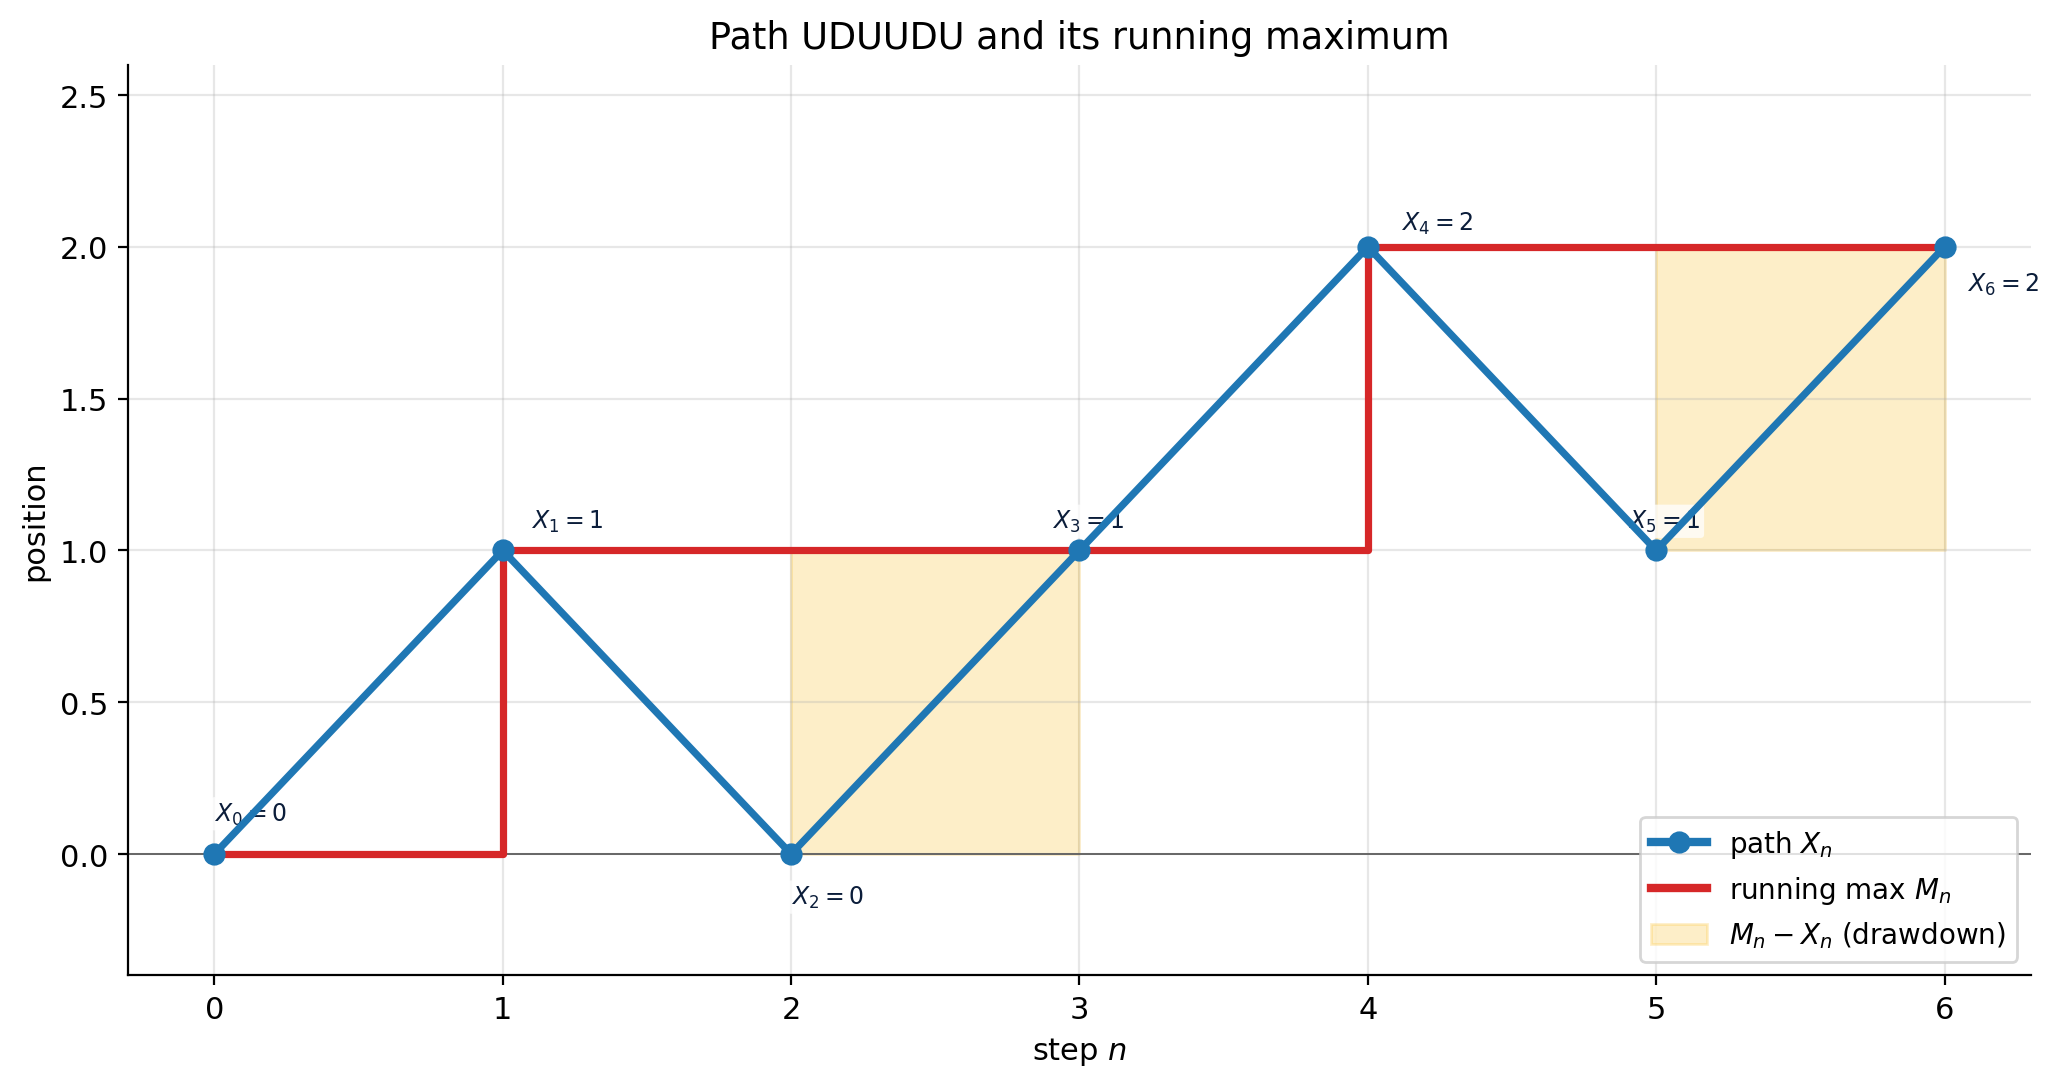
\includegraphics[keepaspectratio]{figures/ch05-running-max-staircase.png}}
\caption{A specific length-6 path (UDUUDU) plotted in blue, with its
running-max staircase \(M_n\) in red. The shaded area is the drawdown
\(M_n - X_n\); it is exactly zero precisely at the times the path
attains a new peak.}
\end{figure}

\begin{figure}
\centering
\pandocbounded{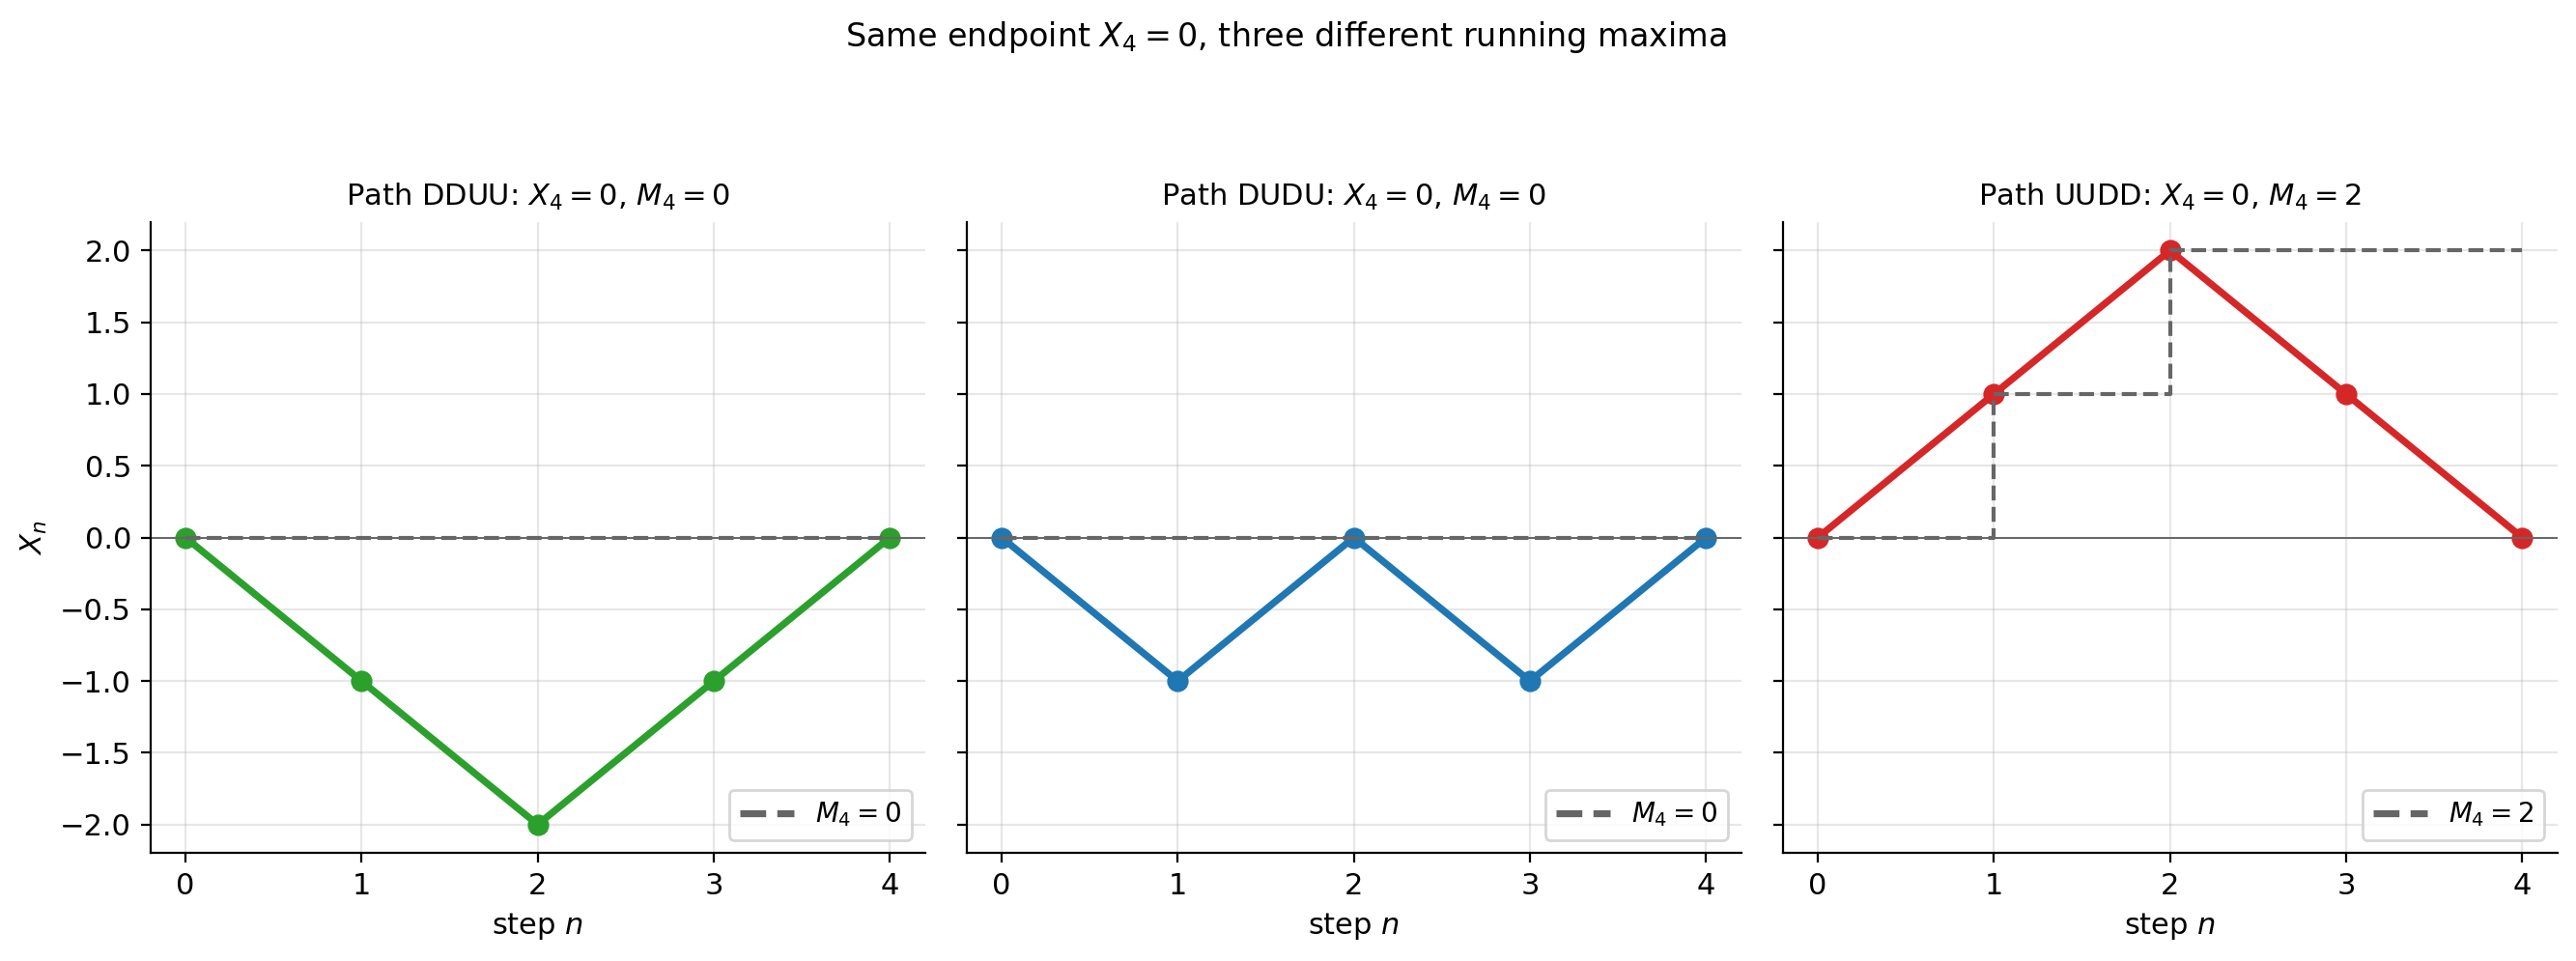
\includegraphics[keepaspectratio]{figures/ch05-three-paths-same-end.png}}
\caption{Three length-4 paths with the same terminal value \(X_4 = 0\)
but different running maxima (\(M_4 = 0, 0, 2\)). The endpoint alone
cannot distinguish them; barrier and lookback payoffs must see the whole
path.}
\end{figure}

\subsection{5.2.3 Tables}\label{tables-12}

\textbf{Table 5.3.} All 16 length-4 paths with their terminal value
\(X_4\) and running max \(M_4\), sorted by \(M_4\).

{\def\LTcaptype{none} % do not increment counter
\begin{table}[H]
\centering
\begin{tabular}{|l|r|r|l|l|r|r|}
\toprule
Path & \(X_4\) & \(M_4\) & & Path & \(X_4\) & \(M_4\) \\
\midrule



DDDD & \(-4\) & \(0\) & & UDUD & \(0\) & \(1\) \\
DDDU & \(-2\) & \(0\) & & UDDU & \(0\) & \(1\) \\
DDUD & \(-2\) & \(0\) & & UDDD & \(-2\) & \(1\) \\
DUDD & \(-2\) & \(0\) & & UUDU & \(+2\) & \(2\) \\
DDUU & \(0\) & \(0\) & & UUDD & \(0\) & \(2\) \\
DUDU & \(0\) & \(0\) & & UDUU & \(+2\) & \(2\) \\
DUUD & \(0\) & \(1\) & & DUUU & \(+2\) & \(2\) \\
& & & & UUUD & \(+2\) & \(3\) \\
& & & & UUUU & \(+4\) & \(4\) \\
\bottomrule
\end{tabular}
\end{table}
}

\textbf{Table 5.4.} Counts of \((X_4, M_4)\) --- the joint distribution
at \(n=4\).

{\def\LTcaptype{none} % do not increment counter
\begin{table}[H]
\centering
\begin{tabular}{|l|r|r|}
\toprule
\((X_4, M_4)\) & count & probability \\
\midrule



\((-4, 0)\) & \(1\) & \(1/16\) \\
\((-2, 0)\) & \(3\) & \(3/16\) \\
\((-2, 1)\) & \(1\) & \(1/16\) \\
\((0, 0)\) & \(2\) & \(2/16\) \\
\((0, 1)\) & \(3\) & \(3/16\) \\
\((0, 2)\) & \(1\) & \(1/16\) \\
\((+2, 2)\) & \(3\) & \(3/16\) \\
\((+2, 3)\) & \(1\) & \(1/16\) \\
\((+4, 4)\) & \(1\) & \(1/16\) \\
total & \(16\) & \(1.000\) \\
\bottomrule
\end{tabular}
\end{table}
}

\subsection{5.2.4 Exercises}\label{exercises-22}

\begin{enumerate}
\def\labelenumi{\arabic{enumi}.}
\tightlist
\item
  From Table 5.4 compute \(\mathbb P(M_4 \ge 2)\). \textbf{Answer:} sum
  of rows with \(M_4 \ge 2\): \(1 + 3 + 1 + 1 = 6\), so
  \(6/16 = 0.375\). (Matches Example 5.2.4.)
\item
  From Table 5.4 compute \(\mathbb E[M_4]\). \textbf{Answer:}
  \((0 \cdot 6 + 1 \cdot 4 + 2 \cdot 4 + 3 \cdot 1 + 4 \cdot 1)/16 = 19/16 = 1.1875\).
\item
  Translate ``\(S_0 = 4\) Toy, barrier \(L = 8\), \(n = 3\), up-and-in''
  into the \(X\) language. \textbf{Answer:} \(m = 1\) on \(X\),
  \(n = 3\). Want \(M_3 \ge 1\). Paths satisfying this: every path
  except DUD, DDU, DDD --- i.e.~five paths, \(5/8\).
\end{enumerate}

\begin{center}\rule{0.5\linewidth}{0.5pt}\end{center}

\section{§5.3 The Reflection Principle --- Slow
Build}\label{the-reflection-principle-slow-build}

\textbf{Punchline.} \emph{For every path of the random walk that ends at
height \(h \le m\) and touches level \(m\), there is exactly one path
that ends at height \(2m - h\). The map between them is geometric: flip
the post-first-hit portion across the horizontal line \(y = m\).}

Equivalent counting statement: \textbf{the number of length-\(n\) paths
with \(M_n \ge m\) and \(X_n = h\) (for \(h \le m\)) equals the number
of length-\(n\) paths with \(X_n = 2m - h\).}

That second sentence is the only statement we actually use to price. The
``flip the path'' geometry is the \emph{proof} --- but only because the
proof is so visual that, once you see it on tiny cases, you will trust
it forever.

\textbf{Intuition.} A path that touches the barrier \(m\) before time
\(n\) has \emph{committed} to a first-passage event. After that
commitment, the rest of the path is a free symmetric walk starting from
\(m\). \emph{Flip every step after the commitment across \(y = m\)} and
you get another valid symmetric walk, ending at the mirror image
\(2m - h\) instead of \(h\). The flip is reversible --- given the
post-flip path, you can recover the original by flipping again. Hence
the bijection.

\textbf{Why this section is long.} Previous chapters of this book (and
most textbooks) state the reflection principle in three lines and move
on. That is a mistake. The principle is \emph{visual}, \emph{easy to
verify by hand for tiny \(n\)}, and \emph{almost always confusing if you
skip the tiny verification}. We will spend the next twelve pages walking
through cases \(n = 3, 4, 5, 6\) in painstaking detail before any
general statement appears.

\subsection{\texorpdfstring{5.3.1 Tiny case: \(n = 3\),
\(m = 2\)}{5.3.1 Tiny case: n = 3, m = 2}}\label{tiny-case-n-3-m-2}

Recall the 8 paths from Example 5.1.1:

{\def\LTcaptype{none} % do not increment counter
\begin{table}[H]
\centering
\begin{tabular}{|l|l|r|r|}
\toprule
Path & Positions \((X_0, X_1, X_2, X_3)\) & \(M_3\) & \(X_3\) \\
\midrule



UUU & \(0, 1, 2, 3\) & \(3\) & \(3\) \\
UUD & \(0, 1, 2, 1\) & \(2\) & \(1\) \\
UDU & \(0, 1, 0, 1\) & \(1\) & \(1\) \\
UDD & \(0, 1, 0, -1\) & \(1\) & \(-1\) \\
DUU & \(0, -1, 0, 1\) & \(1\) & \(1\) \\
DUD & \(0, -1, 0, -1\) & \(0\) & \(-1\) \\
DDU & \(0, -1, -2, -1\) & \(0\) & \(-1\) \\
DDD & \(0, -1, -2, -3\) & \(0\) & \(-3\) \\
\bottomrule
\end{tabular}
\end{table}
}

\textbf{Which paths reach \(+2\) (i.e.~\(M_3 \ge 2\))?} Only UUU and
UUD. \textbf{Two} paths.

Now let's verify the reflection identity for \(m = 2\) and various
\(h\).

\textbf{Sub-claim (\(h = 3\), no flip needed because \(h > m\)):} Paths
with \(X_3 = 3\)? Only UUU. \emph{And} paths with \(M_3 \ge 2\) and
\(X_3 = 3\)? Same --- UUU. Trivially, any path ending at \(+3\) has
already passed \(+2\).

\textbf{Sub-claim (\(h = 1\), the interesting case):} Paths with
\(M_3 \ge 2\) and \(X_3 = 1\)? Only UUD. \textbf{One} path. The
reflection identity says this equals the number of paths with
\(X_3 = 2m - h = 2 \cdot 2 - 1 = 3\). Paths with \(X_3 = 3\): UUU.
\textbf{One} path. ✓ The bijection sends UUD \(\leftrightarrow\) UUU.

Let's \emph{see} the bijection. UUD has positions \(0, 1, 2, 1\). The
first hit of \(m = 2\) is at time \(\tau = 2\). Reflect positions at
times \(> \tau\) across the line \(y = 2\):

\begin{itemize}
\tightlist
\item
  \(X_3 = 1\) (original) reflects to \(2 \cdot 2 - 1 = 3\).
\end{itemize}

So the reflected path is \(0, 1, 2, 3\) --- i.e.~UUU. The reflection
bijection sends UUD to UUU. Reversing: given UUU, where is its ``first
hit of \(+2\)''? At time 2. Reflect positions after time 2 across
\(y = 2\): \(X_3 = 3 \to 2 \cdot 2 - 3 = 1\). We recover UUD. ✓

\textbf{Example 5.3.1 (verifying the bijection on the smallest
non-trivial case).} Original: UUD = \((0, 1, 2, 1)\). Reflected twin:
UUU = \((0, 1, 2, 3)\). Both touch \(m = 2\) at \(\tau = 2\). The first
two steps are identical; the third step is flipped. \emph{That's the
entire principle in three steps.}

\subsection{\texorpdfstring{5.3.2 Case \(n = 4\),
\(m = 2\)}{5.3.2 Case n = 4, m = 2}}\label{case-n-4-m-2}

This is the case that becomes confusing if you don't enumerate. There
are 16 paths total; 6 of them have \(M_4 \ge 2\) (Example 5.2.4). With
parity \(X_4 \in \{-4,-2,0,+2,+4\}\), bucket them by terminal value
(reading off Table 5.4):

{\def\LTcaptype{none} % do not increment counter
\begin{table}[H]
\centering
\begin{tabular}{|r|l|r|}
\toprule
\(X_4\) & paths with \(M_4 \ge 2\) & count \\
\midrule



\(-4\) & (none) & \(0\) \\
\(-2\) & (none) & \(0\) \\
\(\phantom{+}0\) & UUDD & \(1\) \\
\(+2\) & UUDU, UDUU, DUUU, UUUD & \(4\) \\
\(+4\) & UUUU & \(1\) \\
\bottomrule
\end{tabular}
\end{table}
}

Sum: \(0 + 0 + 1 + 4 + 1 = 6\) paths with \(M_4 \ge 2\). ✓

Now the reflection check. For \(h \le m = 2\), the formula says: number
of paths with \(M_4 \ge 2\) and \(X_4 = h\) equals number of paths with
\(X_4 = 2 \cdot 2 - h = 4 - h\).

{\def\LTcaptype{none} % do not increment counter
\begin{table}[H]
\centering
\begin{tabular}{|r|r|r|r|c|}
\toprule
\(h\) & LHS & target \(2m-h\) & RHS & check \\
\midrule



\(-2\) & \(0\) & \(+6\) & \(0\) & ✓ \\
\(0\) & \(1\) & \(+4\) & \(1\) & ✓ \\
\(+2\) & \(4\) & \(+2\) & \(4\) & ✓ \\
\bottomrule
\end{tabular}
\end{table}
}

\emph{Legend:} \textbf{LHS} = paths with \(M_4 \ge 2\) and \(X_4 = h\);
\textbf{RHS} = paths with \(X_4 = 2m - h\). Row \(h = -2\) has RHS
target \(+6\), out of range (\(\binom{4}{k} = 0\)). Row \(h = 0\): only
UUUU. Row \(h = +2\): UUUD, UUDU, UDUU, DUUU.

The case \(h = 2 = m\) (the boundary) gives \(4 = 4\). The case
\(h = 0\) gives \(1 = 1\). ✓

\textbf{Example 5.3.2 (the bijection for \(h = 0\) at \(n = 4\),
\(m = 2\)).} Original: UUDD = \((0, 1, 2, 1, 0)\). First hit of
\(m = 2\) at \(\tau = 2\). Reflect positions after \(\tau\) across
\(y = 2\): \(X_3 = 1 \to 3\), \(X_4 = 0 \to 4\). Reflected path:
\((0, 1, 2, 3, 4)\) --- that's UUUU. ✓ One path on the left, one path on
the right.

\textbf{Example 5.3.3 (the bijection for \(h = +2\) at \(n = 4\),
\(m = 2\)).} We have 4 paths with \(M_4 \ge 2\) and \(X_4 = +2\). Let's
check each.

\begin{enumerate}
\def\labelenumi{\arabic{enumi}.}
\item
  UUUD = \((0, 1, 2, 3, 2)\). First hit of \(m = 2\) at \(\tau = 2\).
  Reflect after \(\tau\): \(X_3 = 3 \to 1\), \(X_4 = 2 \to 2\).
  Reflected: \((0, 1, 2, 1, 2)\) --- i.e.~UUDU. Terminal value \(+2\).
  (At the boundary case \(h = m\) the reflection is a self-bijection on
  \(\{X_n = m\}\), not the identity but a non-trivial involution. For
  \(h > m\) no reflection is needed: every path ending above \(m\) has
  automatically already been at \(m\). The identity gives a strong
  statement only when \(h < m\).)
\item
  UUDU = \((0, 1, 2, 1, 2)\). First hit of \(m = 2\) at \(\tau = 2\).
  Reflect after \(\tau\): \(X_3 = 1 \to 3\), \(X_4 = 2 \to 2\).
  Reflected: \((0, 1, 2, 3, 2)\) --- i.e.~UUUD. (Same pair as case 1,
  reversed.)
\item
  UDUU = \((0, 1, 0, 1, 2)\). First hit of \(m = 2\) at \(\tau = 4\)
  (the last step!). Reflect after \(\tau = 4\): nothing to reflect. The
  reflected path equals UDUU. Terminal value \(X_4 = +2 = m\).
  (Self-image under the bijection.)
\item
  DUUU = \((0, -1, 0, 1, 2)\). First hit of \(m = 2\) at \(\tau = 4\).
  Same situation: self-image.
\end{enumerate}

So at \(h = m\), the bijection pairs UUUD \(\leftrightarrow\) UUDU and
fixes UDUU and DUUU. Count: 4 on each side. ✓

\textbf{The lesson: when \(h < m\) strictly, the bijection moves paths
\emph{out} of \(\{M_n \ge m, X_n = h\}\) and \emph{into}
\(\{X_n = 2m - h\}\), and both these sets are equal because the
bijection is well-defined and invertible.}

\subsection{\texorpdfstring{5.3.3 Case \(n = 5\),
\(m = 3\)}{5.3.3 Case n = 5, m = 3}}\label{case-n-5-m-3}

Now 32 paths. We want \(M_5 \ge 3\).

Paths reaching \(+3\) in \(\le 5\) steps. Direct enumeration (I count by
computer; see also figure below): \textbf{7 paths} with \(M_5 \ge 3\).
Bucketed by terminal value:

{\def\LTcaptype{none} % do not increment counter
\begin{table}[H]
\centering
\begin{tabular}{|r|l|r|}
\toprule
\(X_5\) & paths with \(M_5 \ge 3\) & count \\
\midrule



\(+1\) & UUUDD & \(1\) \\
\(+3\) & UUUDU, UUDUU, UDUUU, DUUUU, UUUUD & \(5\) \\
\(+5\) & UUUUU & \(1\) \\
\bottomrule
\end{tabular}
\end{table}
}

Total \(1 + 5 + 1 = 7\). ✓

Reflection check for \(h = 1 < m = 3\): target is \(2 \cdot 3 - 1 = 5\).
Paths with \(X_5 = 5\): only UUUUU. \textbf{One}. And paths with
\(M_5 \ge 3, X_5 = 1\): only UUUDD. \textbf{One}. ✓

\textbf{Example 5.3.4 (the bijection for \(h = 1\) at \(n = 5\),
\(m = 3\)).} Original: UUUDD = \((0, 1, 2, 3, 2, 1)\). First hit of
\(m = 3\) at \(\tau = 3\). Reflect after \(\tau\): \(X_4 = 2 \to 4\),
\(X_5 = 1 \to 5\). Reflected: \((0, 1, 2, 3, 4, 5)\) --- i.e.~UUUUU. ✓

It is the \emph{only} example of the bijection between
\(\{M_5 \ge 3, X_5 = 1\}\) and \(\{X_5 = 5\}\), because both sets have
exactly one element.

\textbf{Example 5.3.5 (the bijection for \(h = 3\) at \(n = 5\),
\(m = 3\)).} Here \(h = m\), the boundary case. Both sides count ``paths
ending at \(X_5 = 3\)'' which equals 5. The bijection is a
self-involution on the 5 paths. Quick check on one: UUUDU =
\((0, 1, 2, 3, 2, 3)\). First hit \(\tau = 3\). Reflect:
\(X_4 = 2 \to 4\), \(X_5 = 3 \to 3\). Reflected: \((0, 1, 2, 3, 4, 3)\)
--- i.e.~UUUUD. Both UUUDU and UUUUD are in \(\{X_5 = 3\}\). ✓

\begin{figure}
\centering
\pandocbounded{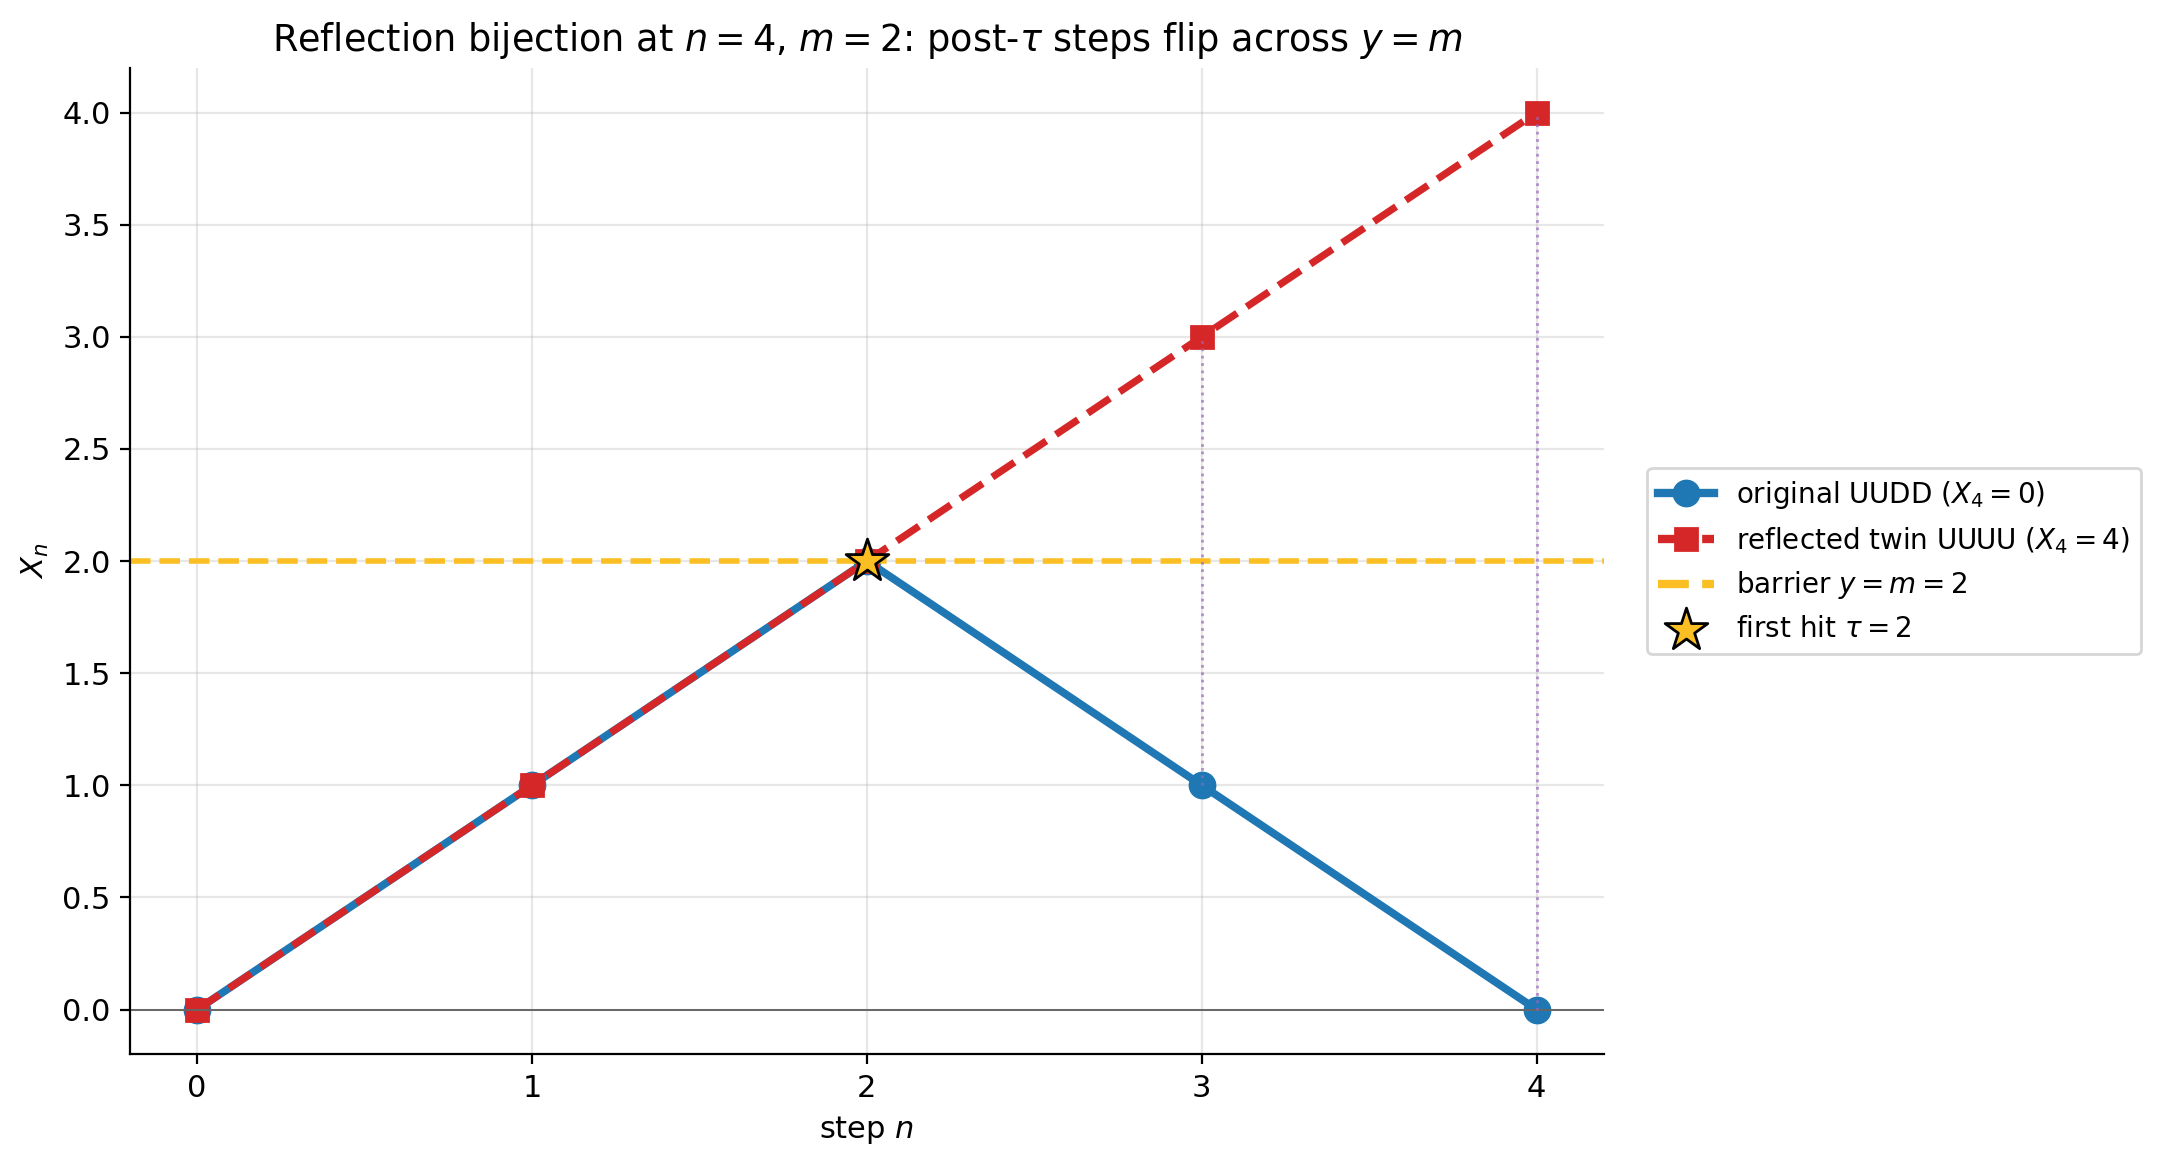
\includegraphics[keepaspectratio]{figures/ch05-reflection-twin.png}}
\caption{Original path UUDD at \(n=4\), \(m=2\) (blue, ends at
\(X_4 = 0\)) and its reflected twin UUUU (red, ends at \(X_4 = 4\)). The
gold star marks the first hit of the barrier at \(\tau = 2\). Every step
\emph{after} \(\tau\) is flipped across \(y = 2\).}
\end{figure}

\begin{figure}
\centering
\pandocbounded{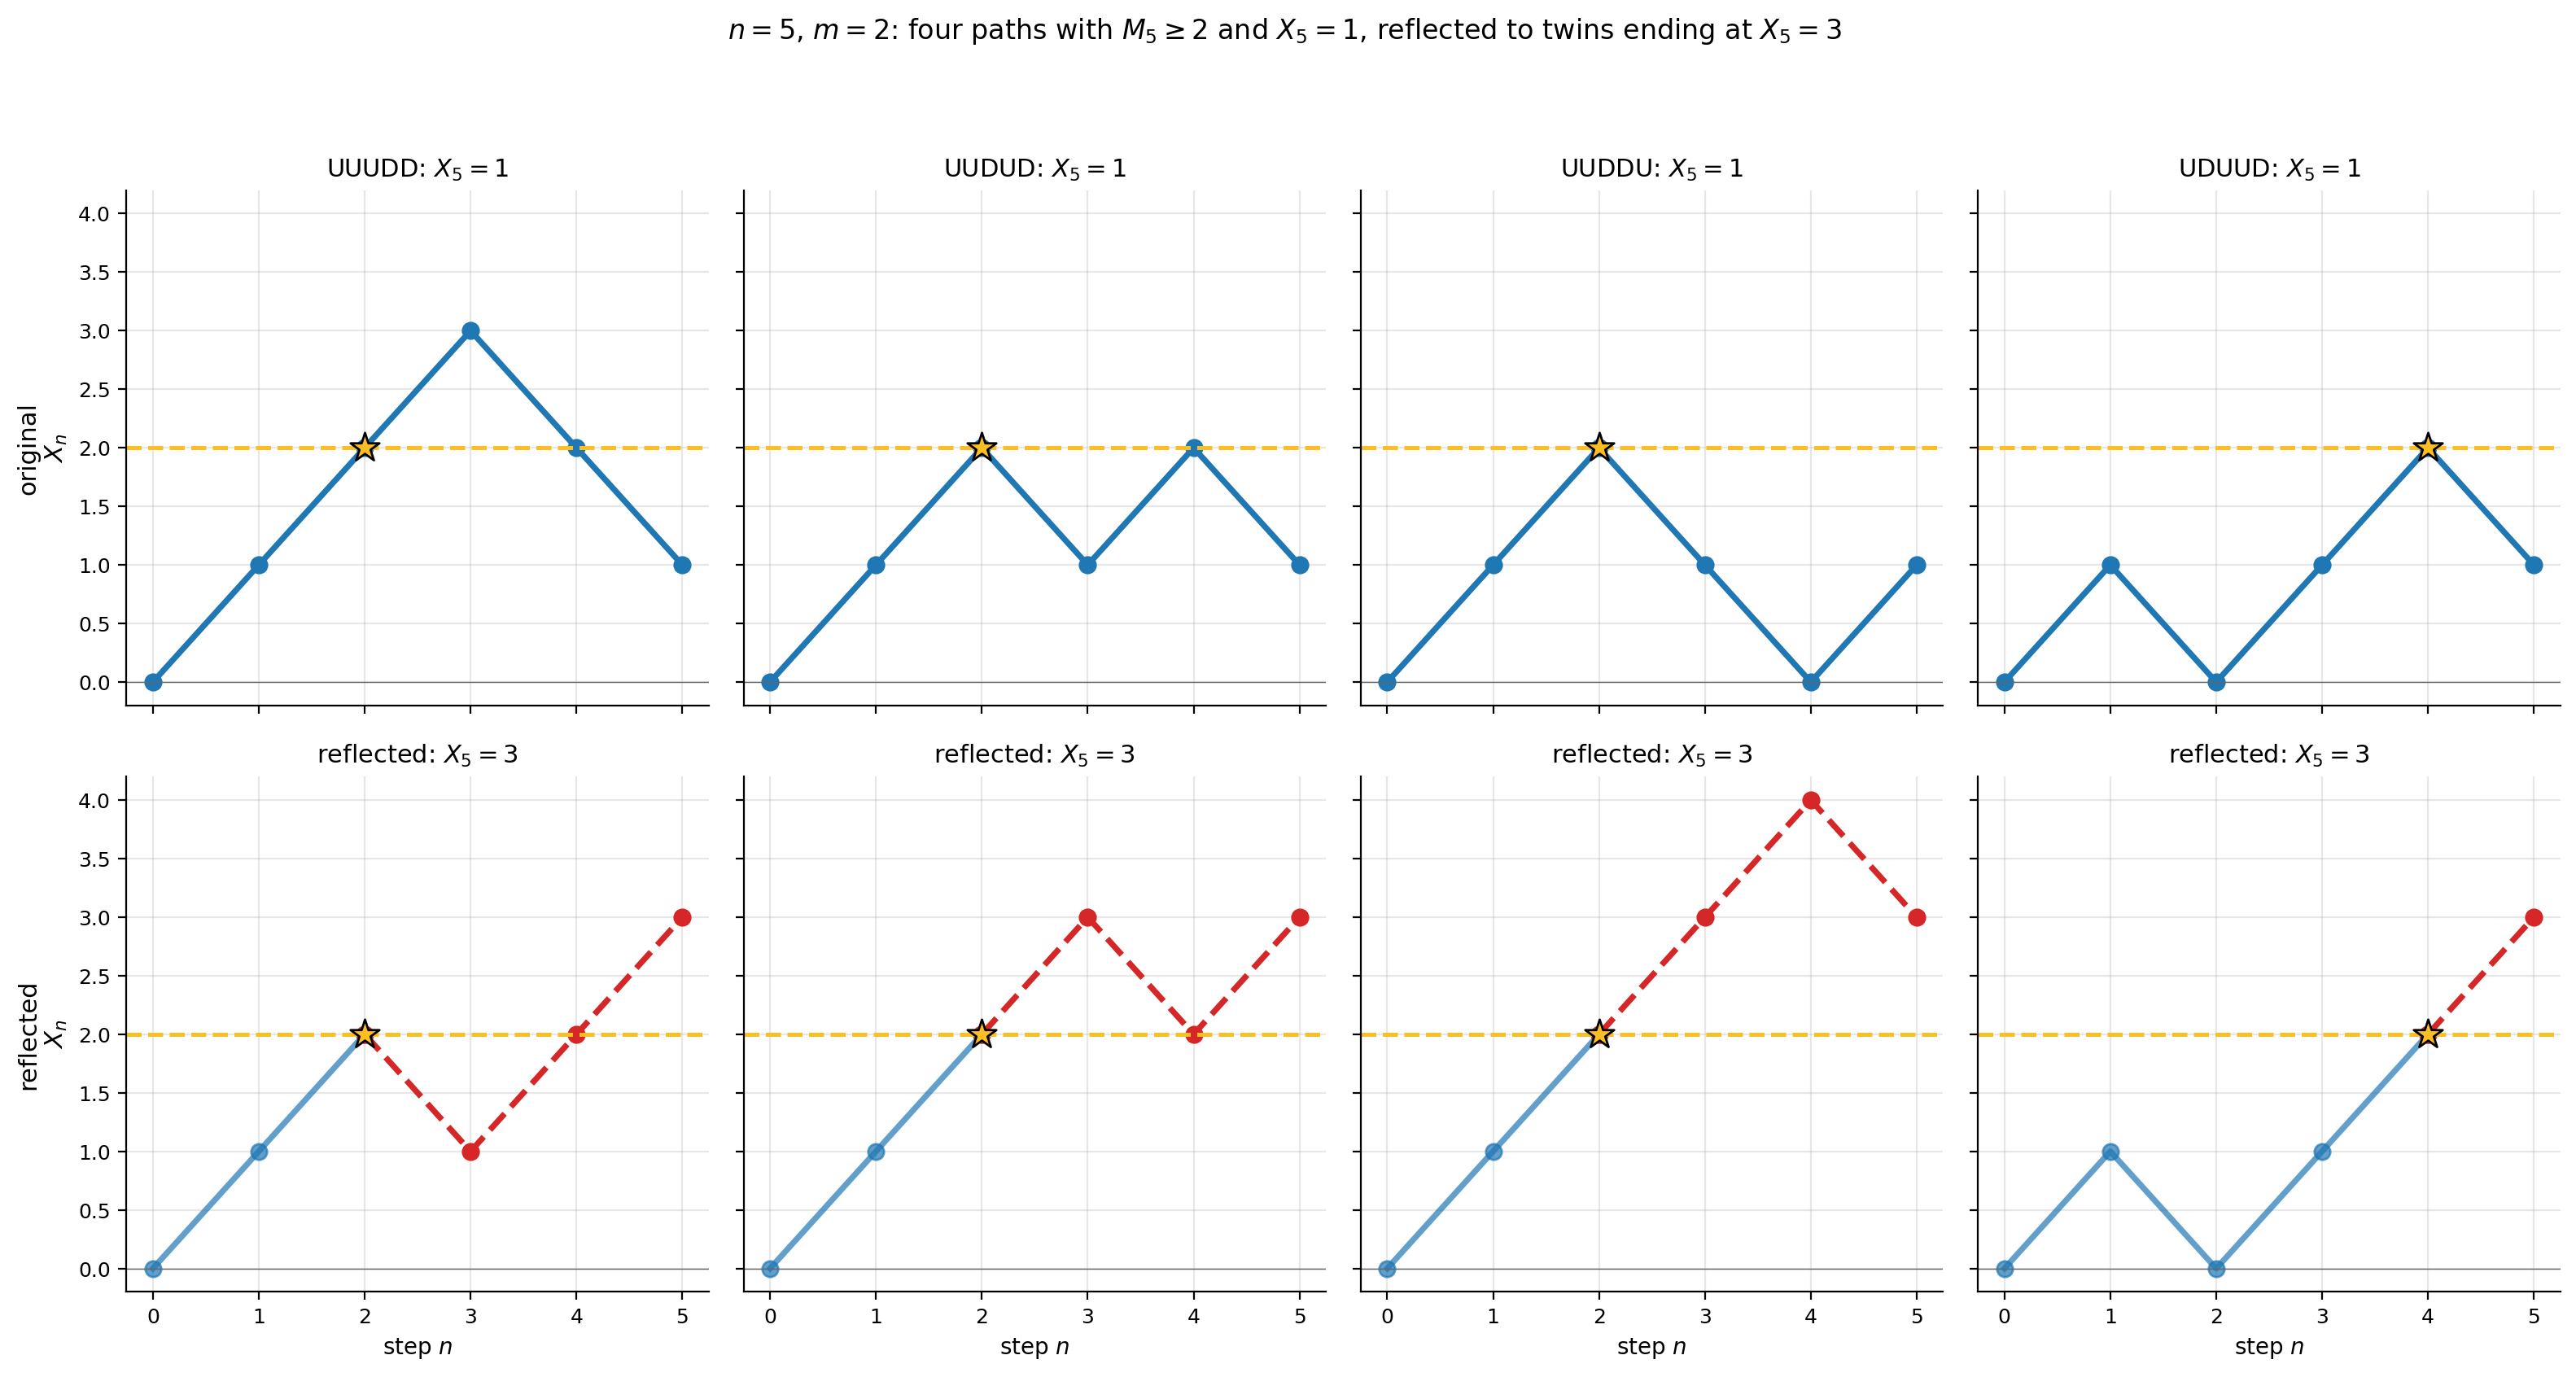
\includegraphics[keepaspectratio]{figures/ch05-length5-pairs-4panel.png}}
\caption{Four length-5 paths with \(M_5 \ge 2\) and \(X_5 = 1\) (top
row), each paired with its reflected twin ending at \(X_5 = 3\) (bottom
row). The first hit of \(m = 2\) is the gold star; before it, the
original and reflected paths are identical. The
reflection-after-\(\tau\) is what swaps endpoints.}
\end{figure}

\subsection{\texorpdfstring{5.3.4 Case \(n = 6\), \(m = 2\),
\(h = 0\)}{5.3.4 Case n = 6, m = 2, h = 0}}\label{case-n-6-m-2-h-0}

The first case big enough that you might not want to enumerate by hand.
We enumerate by computer.

Number of length-6 paths with \(M_6 \ge 2\) and \(X_6 = 0\): \textbf{6}
(by computer-aided enumeration).

Reflection target: \(X_6 = 2 \cdot 2 - 0 = 4\). Number of length-6 paths
with \(X_6 = 4\): choose 5 U's out of 6 steps, so \(\binom{6}{5} = 6\).

So both sides equal 6. ✓

\textbf{Example 5.3.6 (enumerate the 6 paths with \(M_6 \ge 2\) and
\(X_6 = 0\)).} Each such path has exactly 3 U's and 3 D's (forced by
\(X_6 = 0\)) and must touch \(+2\) at some step. Of the
\(\binom{6}{3} = 20\) paths ending at \(X_6 = 0\), only the following
six visit \(+2\):

{\def\LTcaptype{none} % do not increment counter
\begin{table}[H]
\centering
\begin{tabular}{|l|l|r|l|}
\toprule
Original (touches \(+2\), ends at \(0\)) & Positions \((X_0, X_1, \ldots, X_6)\) & First hit \(\tau\) & Reflected twin (ends at \(+4\)) \\
\midrule



UUUDDD & \((0, 1, 2, 3, 2, 1, 0)\) & \(2\) & UUDUUU \\
UUDUDD & \((0, 1, 2, 1, 2, 1, 0)\) & \(2\) & UUUDUU \\
UUDDUD & \((0, 1, 2, 1, 0, 1, 0)\) & \(2\) & UUUUDU \\
UUDDDU & \((0, 1, 2, 1, 0, -1, 0)\) & \(2\) & UUUUUD \\
UDUUDD & \((0, 1, 0, 1, 2, 1, 0)\) & \(4\) & UDUUUU \\
DUUUDD & \((0, -1, 0, 1, 2, 1, 0)\) & \(4\) & DUUUUU \\
\bottomrule
\end{tabular}
\end{table}
}

(In each row, \(\tau\) is the smallest index at which \(X_\tau = 2\).
Reflecting positions strictly after \(\tau\) across the line \(y = 2\)
produces the twin; e.g.~UUUDDD's post-\(\tau\) positions
\((3, 2, 1, 0)\) flip to \((1, 2, 3, 4)\), giving twin positions \$(0,
1, 2, 1, 2, 3, 4) = \$ UUDUUU.) The six reflected twins are precisely
the six length-6 paths with exactly one D, which is \(\binom{6}{5} = 6\)
paths ending at \(X_6 = +4\). The bijection is one-to-one and onto. ✓

So \(|\{M_6 \ge 2, X_6 = 0\}| = 6 = \binom{6}{5} = |\{X_6 = 4\}|\) ---
matching the formula
\(\mathbb P(M_n \ge m, X_n = h) = \mathbb P(X_n = 2m - h)\) at
\((n, m, h) = (6, 2, 0)\).

\begin{figure}
\centering
\pandocbounded{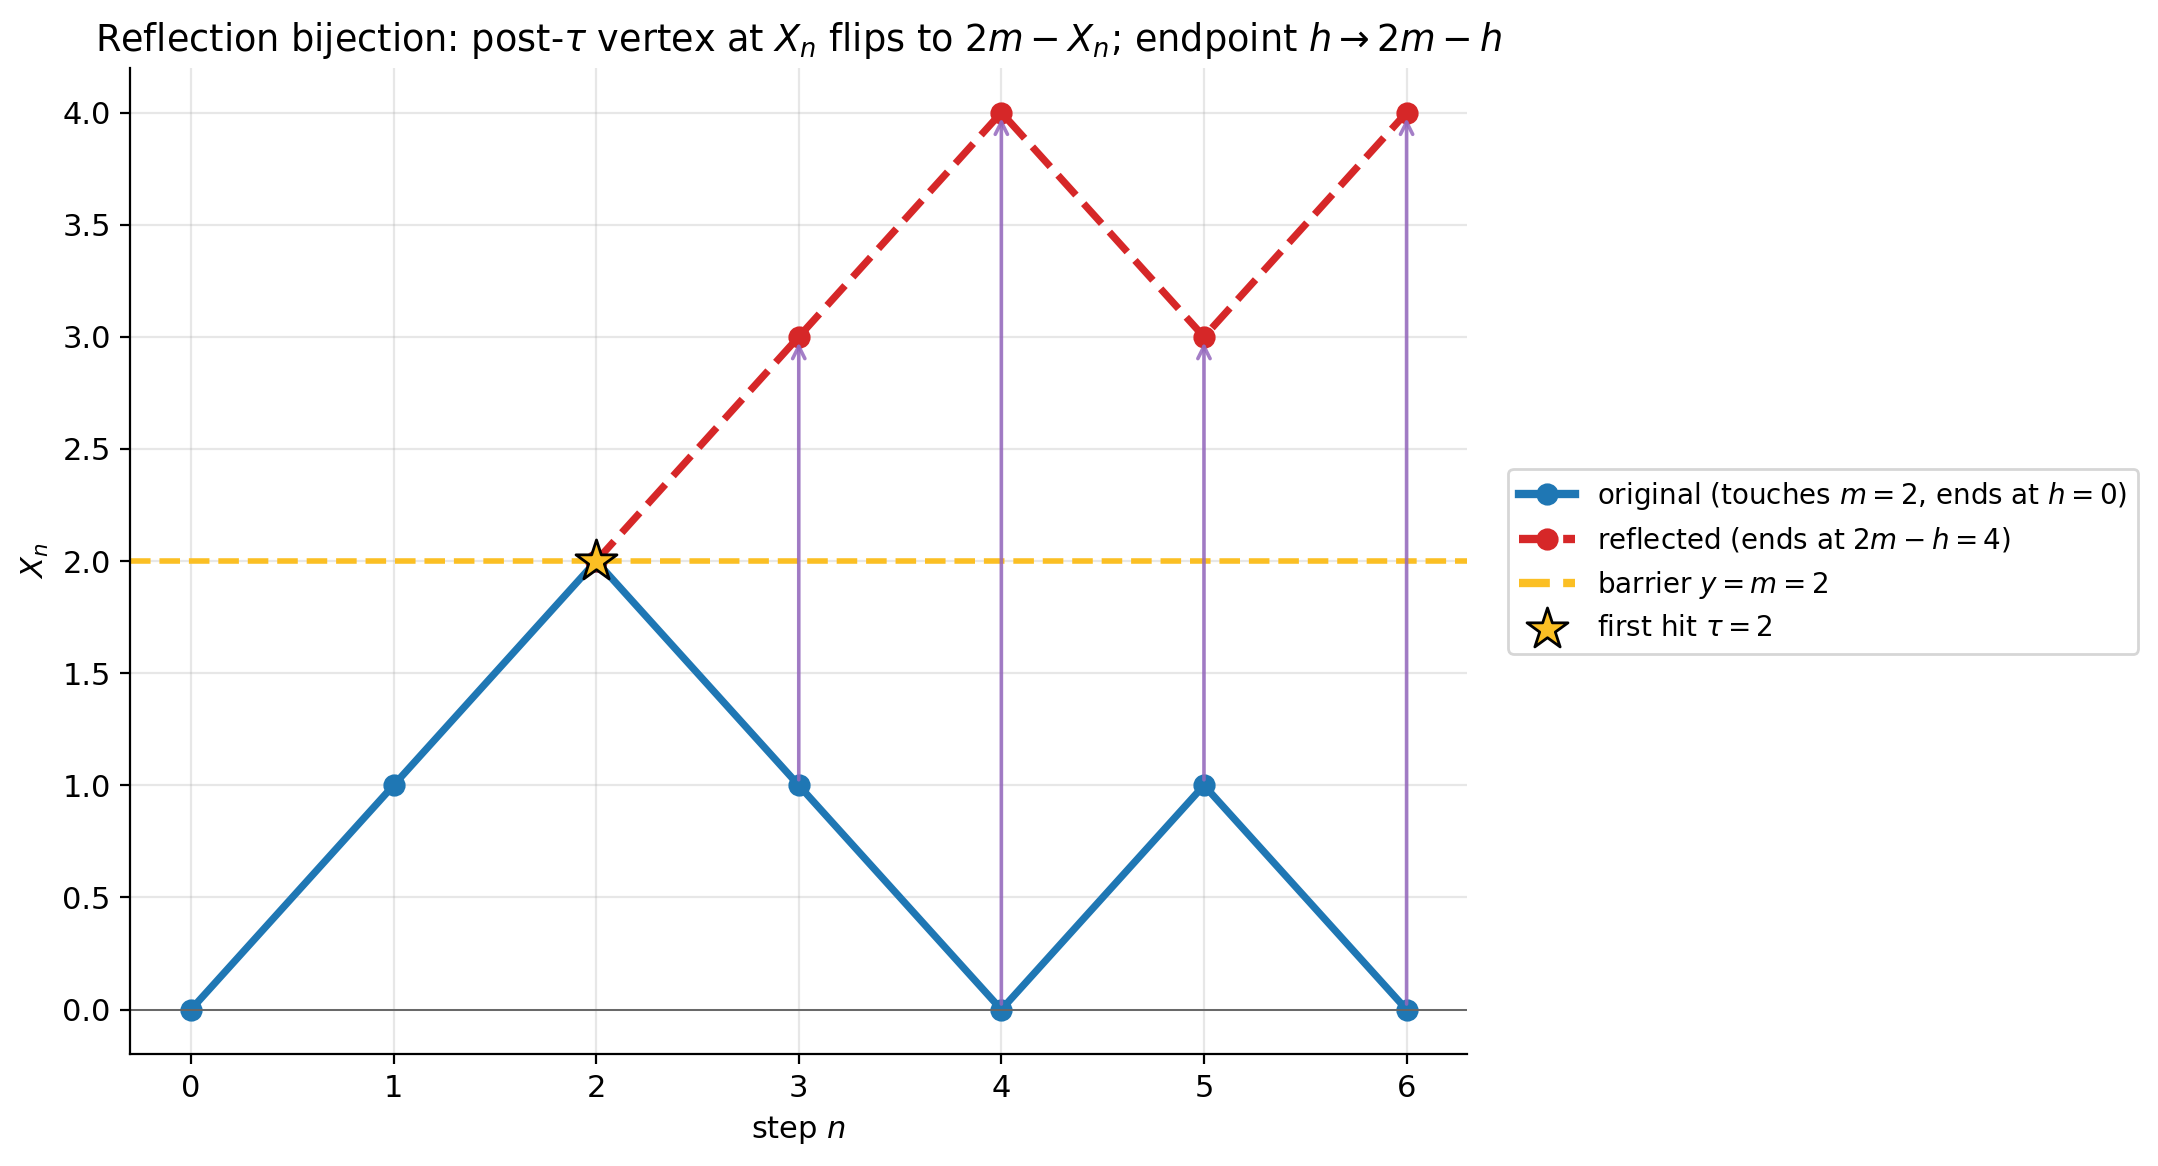
\includegraphics[keepaspectratio]{figures/ch05-bijection-schematic.png}}
\caption{A length-6 path (blue) that touches \(m = 2\) at \(\tau = 2\)
and ends at \(X_6 = 0\), with its reflected twin (red) ending at
\(X_6 = 4\). Purple arrows show how each post-\(\tau\) vertex flips
across \(y = 2\).}
\end{figure}

\begin{figure}
\centering
\pandocbounded{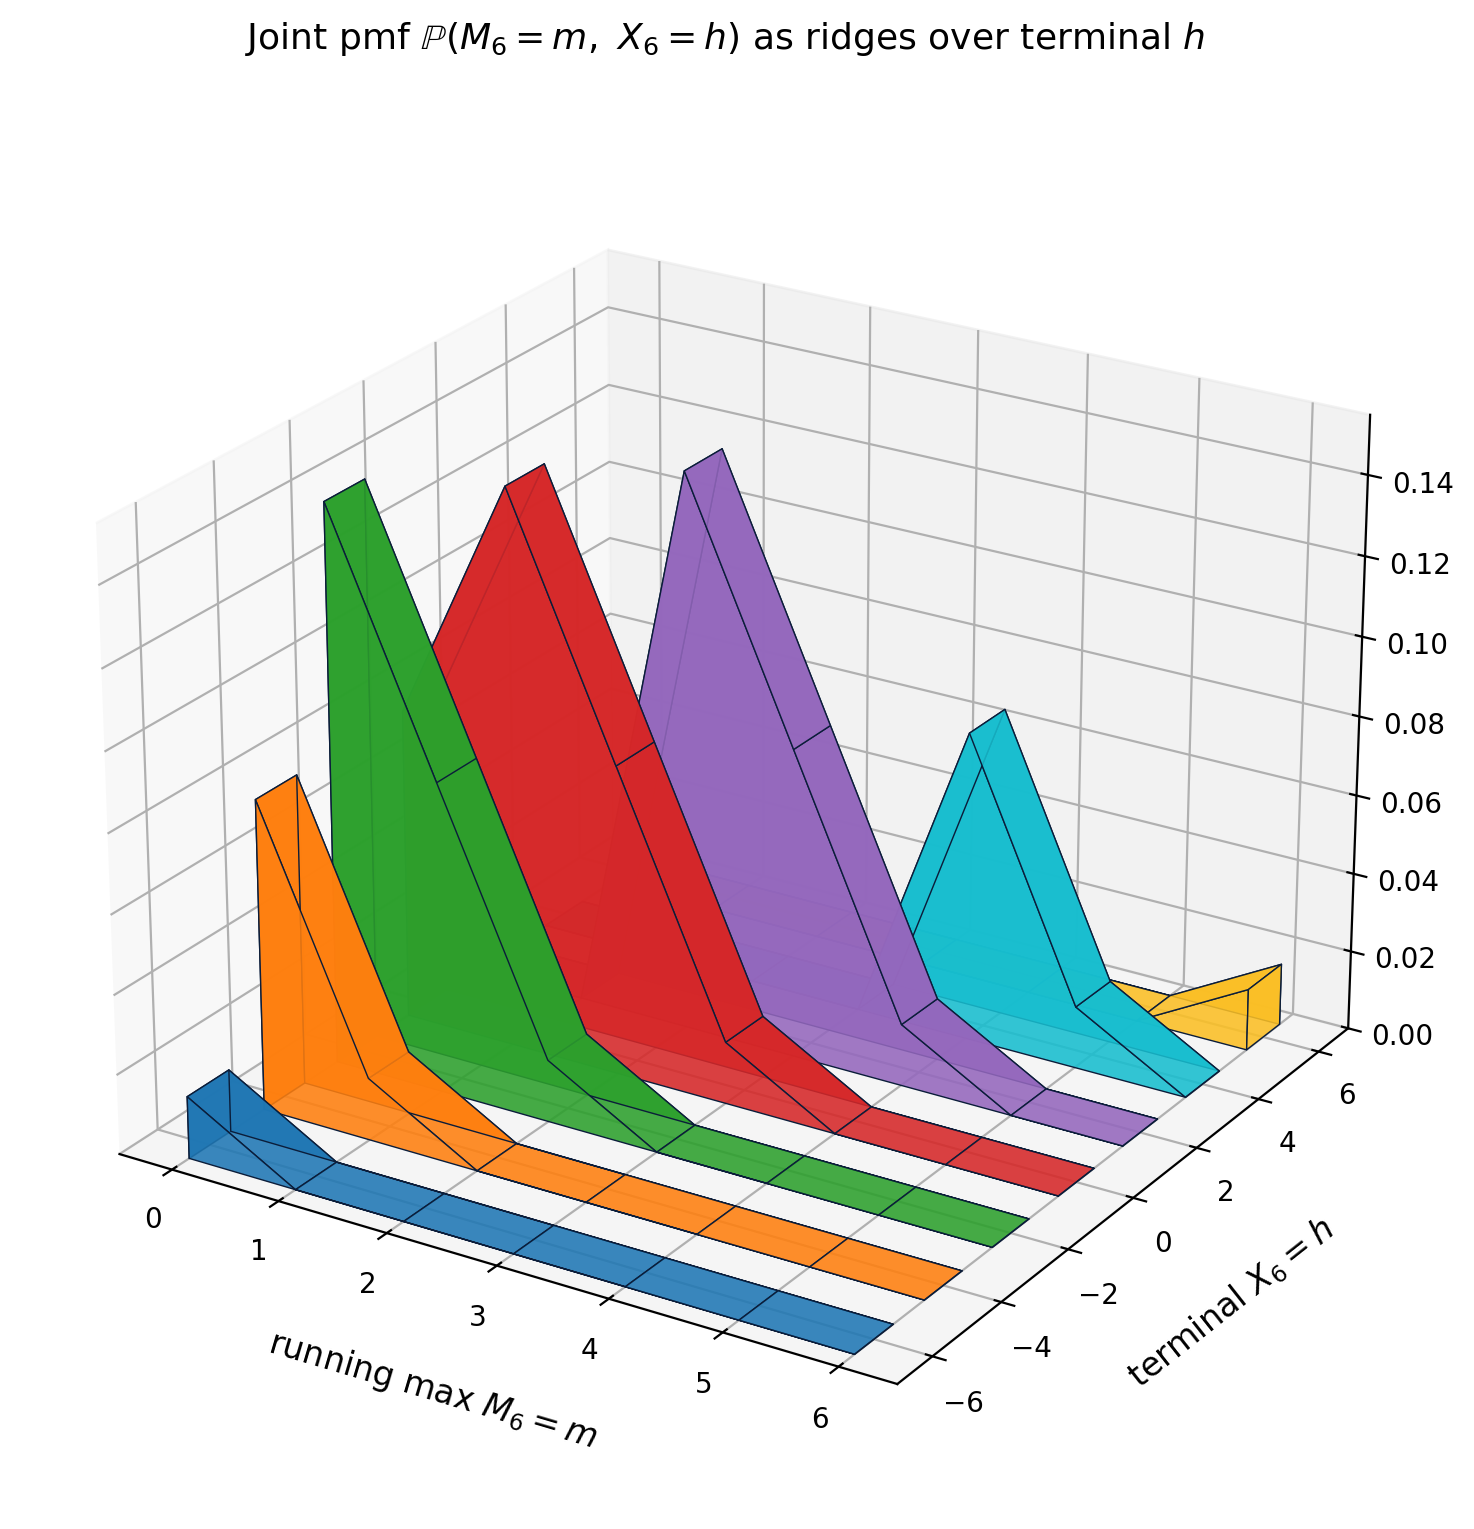
\includegraphics[keepaspectratio]{figures/ch05-joint-bar-n6.png}}
\caption{Empirical joint pmf \(\mathbb P(M_6 \ge 2, X_6 = h)\) from
enumeration over all \(64\) paths (blue bars) overlaid with the
reflection-formula prediction (orange bars). They agree at every \(h\)
--- that's the reflection principle.}
\end{figure}

\subsection{5.3.5 General statement and
corollary}\label{general-statement-and-corollary}

After the four worked cases, we can state the principle.

\textbf{Theorem (Reflection Principle, discrete form).} \emph{Let
\(X_n\) be the symmetric random walk and
\(M_n = \max_{0 \le k \le n} X_k\). For integers \(m \ge 1\) and
\(h \le m\) (with \(h\) having the same parity as \(n\)):}

\[\boxed{\;\mathbb P\bigl(M_n \ge m,\; X_n = h\bigr) \;=\; \mathbb P\bigl(X_n = 2m - h\bigr).\;}\]

Equivalently in counts:
\(|\{M_n \ge m, X_n = h\}| = |\{X_n = 2m - h\}| = \binom{n}{(n + 2m - h)/2}\).

\textbf{Proof sketch.} The map ``flip the path across \(y = m\) after
\(\tau_m\)'' is a bijection between \(\{M_n \ge m, X_n = h\}\) and
\(\{X_n = 2m - h\}\). We verified the construction is well-defined (it
produces a valid \(\pm 1\) walk) and reversible (apply it twice and you
get the original). Since the symmetric walk gives every path probability
\(1/2^n\), the two probabilities are equal.

\textbf{Corollary 1 (marginal for the max --- the ``factor of two''
identity).} \emph{For \(m \ge 1\) (with \(m\) of the same parity as
\(n\)):}

\[\boxed{\;\mathbb P(M_n \ge m) \;=\; 2\,\mathbb P(X_n \ge m) \;-\; \mathbb P(X_n = m).\;}\]

\emph{Derivation.} Split \(\{M_n \ge m\}\) by terminal value:

\[\mathbb P(M_n \ge m) \;=\; \sum_{h \le m}\mathbb P(M_n \ge m,\, X_n = h) \;+\; \sum_{h > m}\mathbb P(X_n = h).\]

(The second sum drops the constraint \(M_n \ge m\) because
\(X_n > m \Rightarrow M_n \ge m\) automatically.) Apply reflection to
the first sum: as \(h\) ranges over \(\{-n, -n+2, \ldots, m\}\), the
reflected value \(2m - h\) ranges over \(\{m, m+2, \ldots, 2m+n\}\). So

\[\sum_{h \le m}\mathbb P(X_n = 2m - h) \;=\; \mathbb P(X_n \ge m).\]

Therefore
\(\mathbb P(M_n \ge m) = \mathbb P(X_n \ge m) + \mathbb P(X_n > m) = 2\mathbb P(X_n \ge m) - \mathbb P(X_n = m)\).
\(\square\)

\textbf{The boundary correction.} The clean continuous-time identity is

\[\mathbb P\bigl(\sup_{0\le t\le T} W_t \ge u\bigr) \;=\; 2\,\mathbb P(W_T \ge u),\]

with no correction term, because \(\mathbb P(W_T = u) = 0\) for the
continuous-density Brownian motion. \emph{In the discrete walk,
\(\mathbb P(X_n = m)\) is a single positive atom --- the ``continuity
correction''} --- and we must subtract it to avoid double-counting paths
that hit \(m\) and finish exactly at \(m\).

\textbf{Equivalent form.} Since \(X_n\) takes only values of the same
parity as \(n\), \(\mathbb P(X_n \ge m+1) = \mathbb P(X_n \ge m+2)\),
and the identity can also be written

\[\mathbb P(M_n \ge m) \;=\; \mathbb P(X_n \ge m) + \mathbb P(X_n \ge m+1).\]

Both forms are equivalent; we will use whichever is cleaner for the
application at hand.

\textbf{Corollary 2 (joint distribution of \(M_n\) and \(X_n\)).}
Differencing on \(m\):

\[\boxed{\;\mathbb P(M_n = m, X_n = h) \;=\; \mathbb P(X_n = 2m - h) - \mathbb P(X_n = 2m - h + 2).\;}\]

(Valid for \(0 \le m\) and \(h \le m\). The second term comes from
differencing \(\mathbb P(M_n \ge m)\) vs \(\mathbb P(M_n \ge m + 1)\).)

\subsection{5.3.6 More examples using the
formula}\label{more-examples-using-the-formula}

\textbf{Example 5.3.7 (\(\mathbb P(M_{10} \ge 4)\)).}

\[\mathbb P(M_{10} \ge 4) = \mathbb P(X_{10} \ge 4) + \mathbb P(X_{10} \ge 5).\]

For \(X_{10}\), \(\mathbb P(X_{10} = k) = \binom{10}{(10+k)/2}/2^{10}\)
for even \(k\) matching parity, and zero otherwise. So \(X_{10}\) takes
only even values, and \(X_{10} \ge 4\) corresponds to:
\(X_{10} = 4 \Rightarrow 7\) ups, \(\binom{10}{7} = 120\);
\(X_{10} = 6 \Rightarrow 8\) ups, \(\binom{10}{8} = 45\);
\(X_{10} = 8 \Rightarrow \binom{10}{9} = 10\);
\(X_{10} = 10 \Rightarrow \binom{10}{10} = 1\).

\(\mathbb P(X_{10} \ge 4) = (120 + 45 + 10 + 1)/1024 = 176/1024 = 0.1719\).

For \(X_{10} \ge 5\): only \(X_{10} = 6, 8, 10\) (parity skips
\(5, 7, 9\)): \((45 + 10 + 1)/1024 = 56/1024 = 0.0547\).

So \(\mathbb P(M_{10} \ge 4) = 0.1719 + 0.0547 = 0.2266\). (Computer
verification: \(0.2266\). ✓)

\textbf{Example 5.3.8 (\(\mathbb P(M_8 \ge 2)\), two ways).}

\emph{Reflection:}
\(\mathbb P(M_8 \ge 2) = \mathbb P(X_8 \ge 2) + \mathbb P(X_8 \ge 3)\).
Note \(X_8\) is always even, so
\(\mathbb P(X_8 \ge 3) = \mathbb P(X_8 \ge 4)\).

\(\mathbb P(X_8 \ge 2) = (\binom{8}{5} + \binom{8}{6} + \binom{8}{7} + \binom{8}{8})/256 = (56 + 28 + 8 + 1)/256 = 93/256\).

\(\mathbb P(X_8 \ge 4) = (28 + 8 + 1)/256 = 37/256\).

Sum: \(93 + 37 = 130\), so \(\mathbb P(M_8 \ge 2) = 130/256 = 0.5078\).

\emph{Enumeration:} exhaustively check all \(2^8 = 256\) paths and count
those with \(\max X_k \ge 2\). Computer says \(130\). ✓

\textbf{Example 5.3.9 (the joint formula at \(n = 6, m = 2, h = 0\)).}

\(\mathbb P(M_6 = 2, X_6 = 0) = \mathbb P(X_6 = 4) - \mathbb P(X_6 = 6) = \binom{6}{5}/64 - \binom{6}{6}/64 = 6/64 - 1/64 = 5/64\).

Cross-check: enumeration over all 64 paths gives 6 paths with
\(M_6 \ge 2\) and \(X_6 = 0\), decomposing as \((M_6, X_6) = (2, 0)\): 5
paths, plus \((M_6, X_6) = (3, 0)\): 1 path. \(5 + 1 = 6\). ✓

\subsection{5.3.7 Tables}\label{tables-13}

\textbf{Table 5.5.} Bijection for \(n = 3\), \(m = 2\). Each row pairs a
path with \(M_3 \ge 2, X_3 = h\) (for \(h \le m\)) with its reflected
twin ending at \(2m - h\).

{\def\LTcaptype{none} % do not increment counter
\begin{table}[H]
\centering
\begin{tabular}{|l|r|r|l|r|}
\toprule
Original & \(X_3\) & \(\tau\) & Reflected & \(X_3\) \\
\midrule



UUD & \(+1\) & \(2\) & UUU & \(+3\) \\
\bottomrule
\end{tabular}
\end{table}
}

Only one pair, since \(|\{M_3 \ge 2, X_3 = 1\}| = |\{X_3 = 3\}| = 1\).

\textbf{Table 5.6.} Bijection for \(n = 4\), \(m = 2\). For
\(h < m = 2\) (i.e.~\(h \in \{-2, 0\}\)):

{\def\LTcaptype{none} % do not increment counter
\begin{table}[H]
\centering
\begin{tabular}{|l|r|l|}
\toprule
Original \(X_4 = h\) & \(\tau\) & Reflected \(X_4 = 2m - h\) \\
\midrule



(none with \(X_4 = -2\) and \(M_4 \ge 2\)) & & \\
UUDD (\(h = 0\)) & \(2\) & UUUU (\(X_4 = 4\)) \\
\bottomrule
\end{tabular}
\end{table}
}

\emph{Blank: empty set, no path to reflect.}

Plus boundary \(h = m = 2\) (self-bijection on the 4 paths with
\(X_4 = 2\), namely UUUD \(\leftrightarrow\) UUDU, UDUU
\(\leftrightarrow\) UDUU, DUUU \(\leftrightarrow\) DUUU).

\textbf{Table 5.7.} Joint counts \(\lvert\{M_5 \ge 3, X_5 = h\}\rvert\)
vs reflected counts \(\lvert\{X_5 = 2 \cdot 3 - h\}\rvert\).

{\def\LTcaptype{none} % do not increment counter
\begin{table}[H]
\centering
\begin{tabular}{|r|r|r|r|}
\toprule
\(h\) & LHS count & \(2m - h\) & RHS count \\
\midrule



\(-5\) & \(0\) & \(11\) & \(0\) \\
\(-3\) & \(0\) & \(9\) & \(0\) \\
\(-1\) & \(0\) & \(7\) & \(0\) \\
\(+1\) & \(1\) & \(5\) & \(1\) \\
\(+3\) & \(5\) & \(3\) & \(5\) \\
\(+5\) & \(1\) & \(1\) & \(1\) \\
\bottomrule
\end{tabular}
\end{table}
}

\emph{Legend:} \textbf{LHS count} =
\(\lvert\{M_5 \ge 3, X_5 = h\}\rvert\); \textbf{RHS count} =
\(\lvert\{X_5 = 2m - h\}\rvert\) with \(m = 3\).

All rows balance.

\begin{center}\rule{0.5\linewidth}{0.5pt}\end{center}

\section{§5.4 First-passage times}\label{first-passage-times}

\textbf{Punchline.} The first-passage time
\(\tau_m = \min\{n : X_n = m\}\) has a one-line distribution derived
from the reflection principle:

\[\boxed{\;\mathbb P(\tau_m = n) \;=\; \frac{m}{n}\,\mathbb P(X_n = m) \;=\; \frac{m}{n}\cdot\frac{1}{2^n}\binom{n}{(n+m)/2}.\;}\]

\textbf{Intuition.} A path that \emph{first} hits \(m\) at time \(n\) is
one that hits \(m\) at time \(n\) AND has not hit \(m\) before. To use
reflection, count ``hits \(m\) at time \(n\)'' via paths ending at
\(X_n = m\), then subtract the paths that hit \(m\) at some earlier
time. The bookkeeping collapses to the clean fraction \(m/n\) times the
unconditional density.

\subsection{5.4.1 Derivation (informal)}\label{derivation-informal}

Among paths with \(X_n = m\), some have already touched \(m\) before
time \(n\) (and possibly fallen back). We want only the ``first-time''
hitters at exactly time \(n\). The reflection principle says:

\[\#\{\tau_m = n,\, X_n = m\} = \#\{X_n = m\} - \#\{\tau_m < n,\, X_n = m\}.\]

A path with \(\tau_m < n\) and \(X_n = m\) has, on its last step (step
\(n\)), gone from \(X_{n-1}\) to \(X_n = m\) --- so \(X_{n-1} = m - 1\)
(down-step to \(m\)) or \(X_{n-1} = m + 1\) (down-step from
above\ldots{} but a down-step from \(m+1\) to \(m\) means another hit,
not the \emph{first}). The combinatorics ends with:

\[\mathbb P(\tau_m = n) = \frac{m}{n} \cdot \mathbb P(X_n = m).\]

This is sometimes called the \textbf{ballot theorem} in the
combinatorics literature.

\subsection{5.4.2 Examples}\label{examples-25}

\textbf{Example 5.4.1 (\(\mathbb P(\tau_2 = 4)\)).}

\emph{Formula:}
\((2/4) \cdot \mathbb P(X_4 = 2) = (1/2) \cdot (4/16) = 2/16 = 1/8 = 0.125\).

\emph{Enumeration:} paths of length 4 that reach \(+2\) for the first
time at step 4. The path must have \(X_4 = 2\) and not visit \(+2\)
before. With \(X_4 = 2\) we have 3 U's and 1 D among 4 steps. The 4
candidates: UUUD, UUDU, UDUU, DUUU. Now check first-visit-time of
\(+2\):

\begin{itemize}
\tightlist
\item
  UUUD: \(0, 1, 2, 3, 2\). First hit at \(\tau = 2\). Not \(= 4\).
\item
  UUDU: \(0, 1, 2, 1, 2\). First hit at \(\tau = 2\). Not \(= 4\).
\item
  UDUU: \(0, 1, 0, 1, 2\). First hit at \(\tau = 4\). ✓
\item
  DUUU: \(0, -1, 0, 1, 2\). First hit at \(\tau = 4\). ✓
\end{itemize}

Two paths satisfy \(\tau_2 = 4\). \(\mathbb P = 2/16 = 1/8\). ✓

\textbf{Example 5.4.2 (\(\mathbb P(\tau_3 = 5)\)).}

\emph{Formula:}
\((3/5) \cdot \mathbb P(X_5 = 3) = (3/5) \cdot (5/32) = 3/32 = 0.09375\).

\emph{Enumeration:} \(X_5 = 3\) requires 4 U's, 1 D, so 5 candidates. We
need the ones that don't reach \(+3\) before step 5.

\begin{itemize}
\tightlist
\item
  UUUUD: \(0,1,2,3,4,3\). \(\tau_3 = 3\). No.
\item
  UUUDU: \(0,1,2,3,2,3\). \(\tau_3 = 3\). No.
\item
  UUDUU: \(0,1,2,1,2,3\). \(\tau_3 = 5\). ✓
\item
  UDUUU: \(0,1,0,1,2,3\). \(\tau_3 = 5\). ✓
\item
  DUUUU: \(0,-1,0,1,2,3\). \(\tau_3 = 5\). ✓
\end{itemize}

Three paths satisfy \(\tau_3 = 5\). \(\mathbb P = 3/32\). ✓

\textbf{Example 5.4.3 (\(\mathbb P(\tau_1 = n)\) for small \(n\)).}
Formula:
\((1/n) \cdot \mathbb P(X_n = 1) = (1/n) \cdot \binom{n}{(n+1)/2}/2^n\),
defined only for odd \(n\).

\begin{itemize}
\tightlist
\item
  \(n = 1\): \(1 \cdot \binom{1}{1}/2 = 1/2\).
\item
  \(n = 3\): \((1/3) \cdot \binom{3}{2}/8 = (1/3)(3/8) = 1/8\).
\item
  \(n = 5\): \((1/5)(10/32) = 2/32 = 1/16\).
\item
  \(n = 7\): \((1/7)(35/128) = 5/128\).
\end{itemize}

Summing:
\(\mathbb P(\tau_1 < \infty) = \sum_{n \text{ odd}} \mathbb P(\tau_1 = n) = 1/2 + 1/8 + 1/16 + 5/128 + \ldots = 1\).
\emph{The walk hits \(+1\) eventually with probability 1.}

\textbf{Example 5.4.4 (\(\mathbb E[\tau_1]\) is infinite).} Even though
the walk hits \(+1\) with probability 1, the \emph{expected time to do
so} is infinite. The sum \(\sum_n n \cdot \mathbb P(\tau_1 = n)\)
diverges --- \(\mathbb P(\tau_1 = n) \sim c/n^{3/2}\), so
\(n \cdot \mathbb P(\tau_1 = n) \sim c/n^{1/2}\) which is non-summable.
\emph{Random walks are recurrent but slowly so.} This is one of the more
surprising facts in elementary probability: an event certain to happen
can have infinite expected waiting time.

\textbf{Example 5.4.5 (ballot problem).} A version of the ballot
theorem: in a counting where candidate A gets \(a\) votes and B gets
\(b\) votes with \(a > b\), the probability that A is \emph{always
ahead} during the count is \((a - b)/(a + b)\). This is exactly
\(\mathbb P(\tau_{-1} > n)\) for a walk that ends at \(X_n = a - b\),
with appropriate translation. The reflection principle is the proof. See
Feller (1968) for the classical writeup.

\textbf{Example 5.4.6 (a long wait).}
\(\mathbb P(\tau_1 = 11) = (1/11) \binom{11}{6}/2^{11} = (1/11)(462/2048) = 42/2048 = 0.0205\).
Compared to \(\mathbb P(\tau_1 = 1) = 1/2\), the probability of waiting
\emph{exactly} 11 flips to first see \(+1\) is small but nontrivial ---
and the \emph{tail} \(\sum_{n > 11}\) is even larger.

\begin{figure}
\centering
\pandocbounded{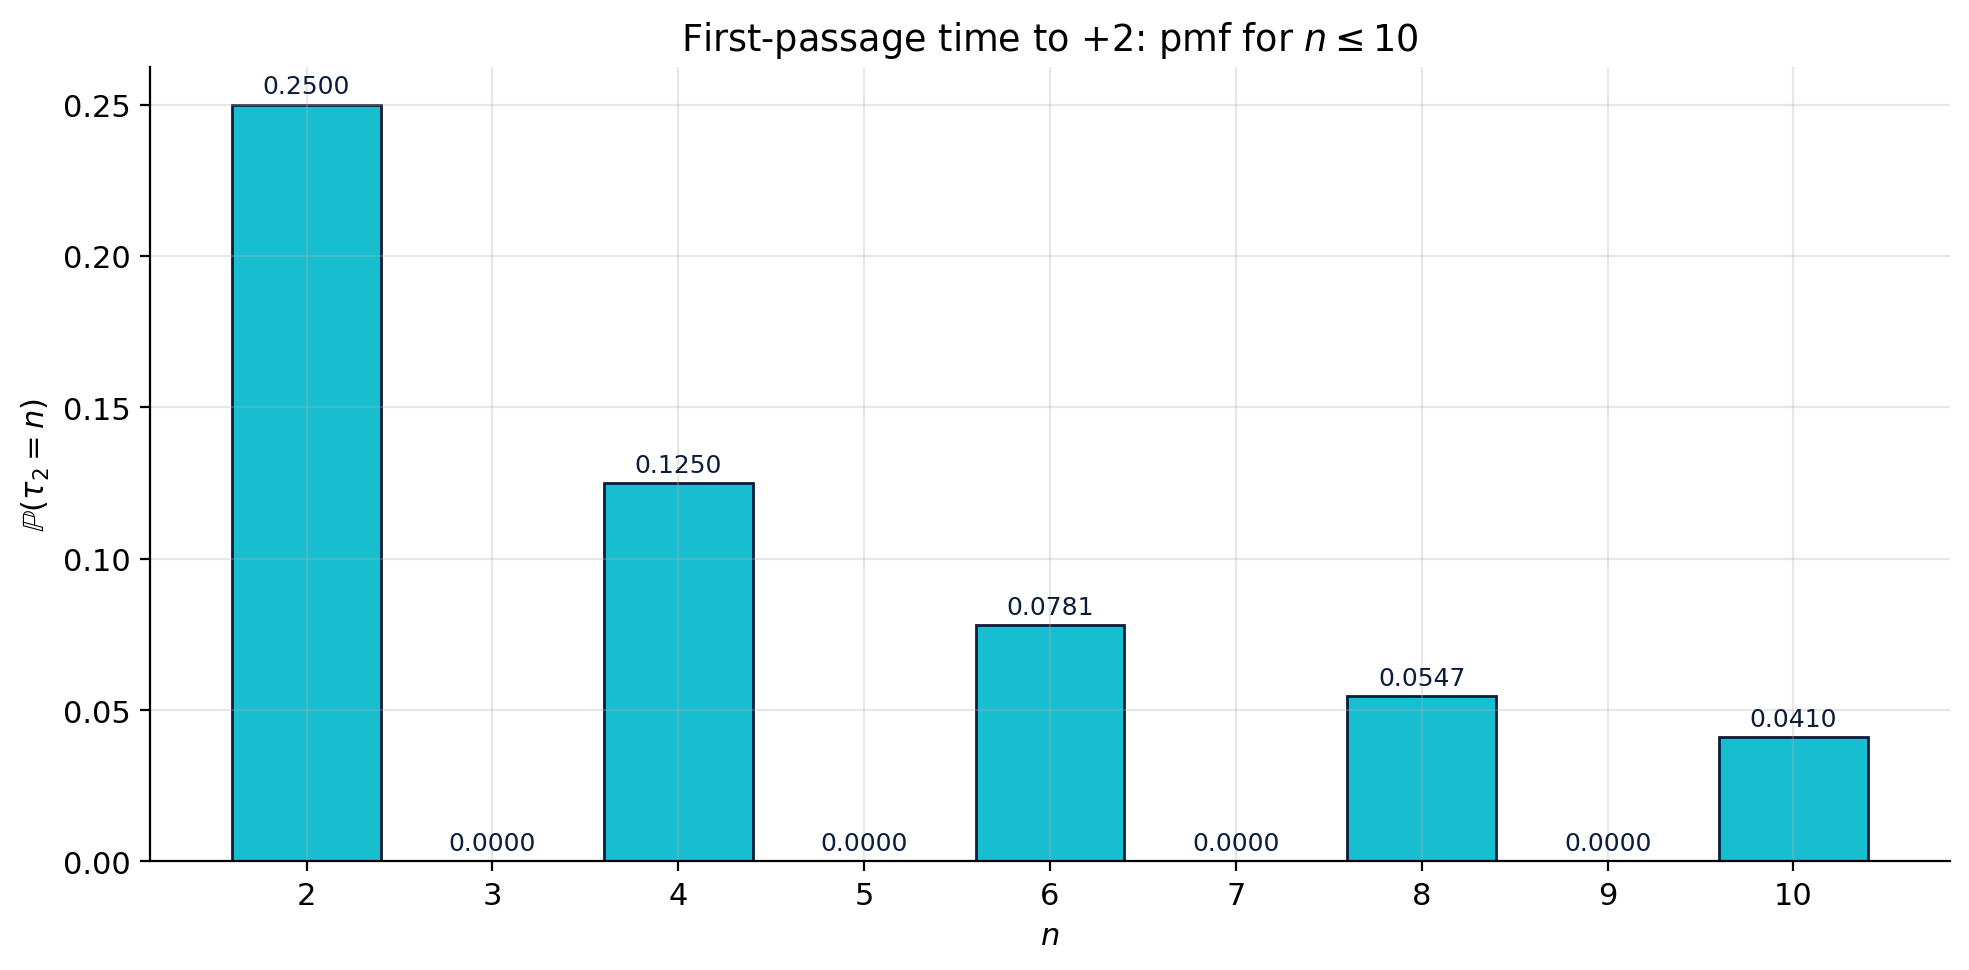
\includegraphics[keepaspectratio]{figures/ch05-tau-hist.png}}
\caption{Probability mass function \(\mathbb P(\tau_2 = n)\) for
\(n \le 10\). The pmf is nonzero only at even \(n \ge 2\). The values
are \(1/4, 1/8, 5/64, 7/128, 21/512\) for \(n = 2, 4, 6, 8, 10\).}
\end{figure}

\begin{figure}
\centering
\pandocbounded{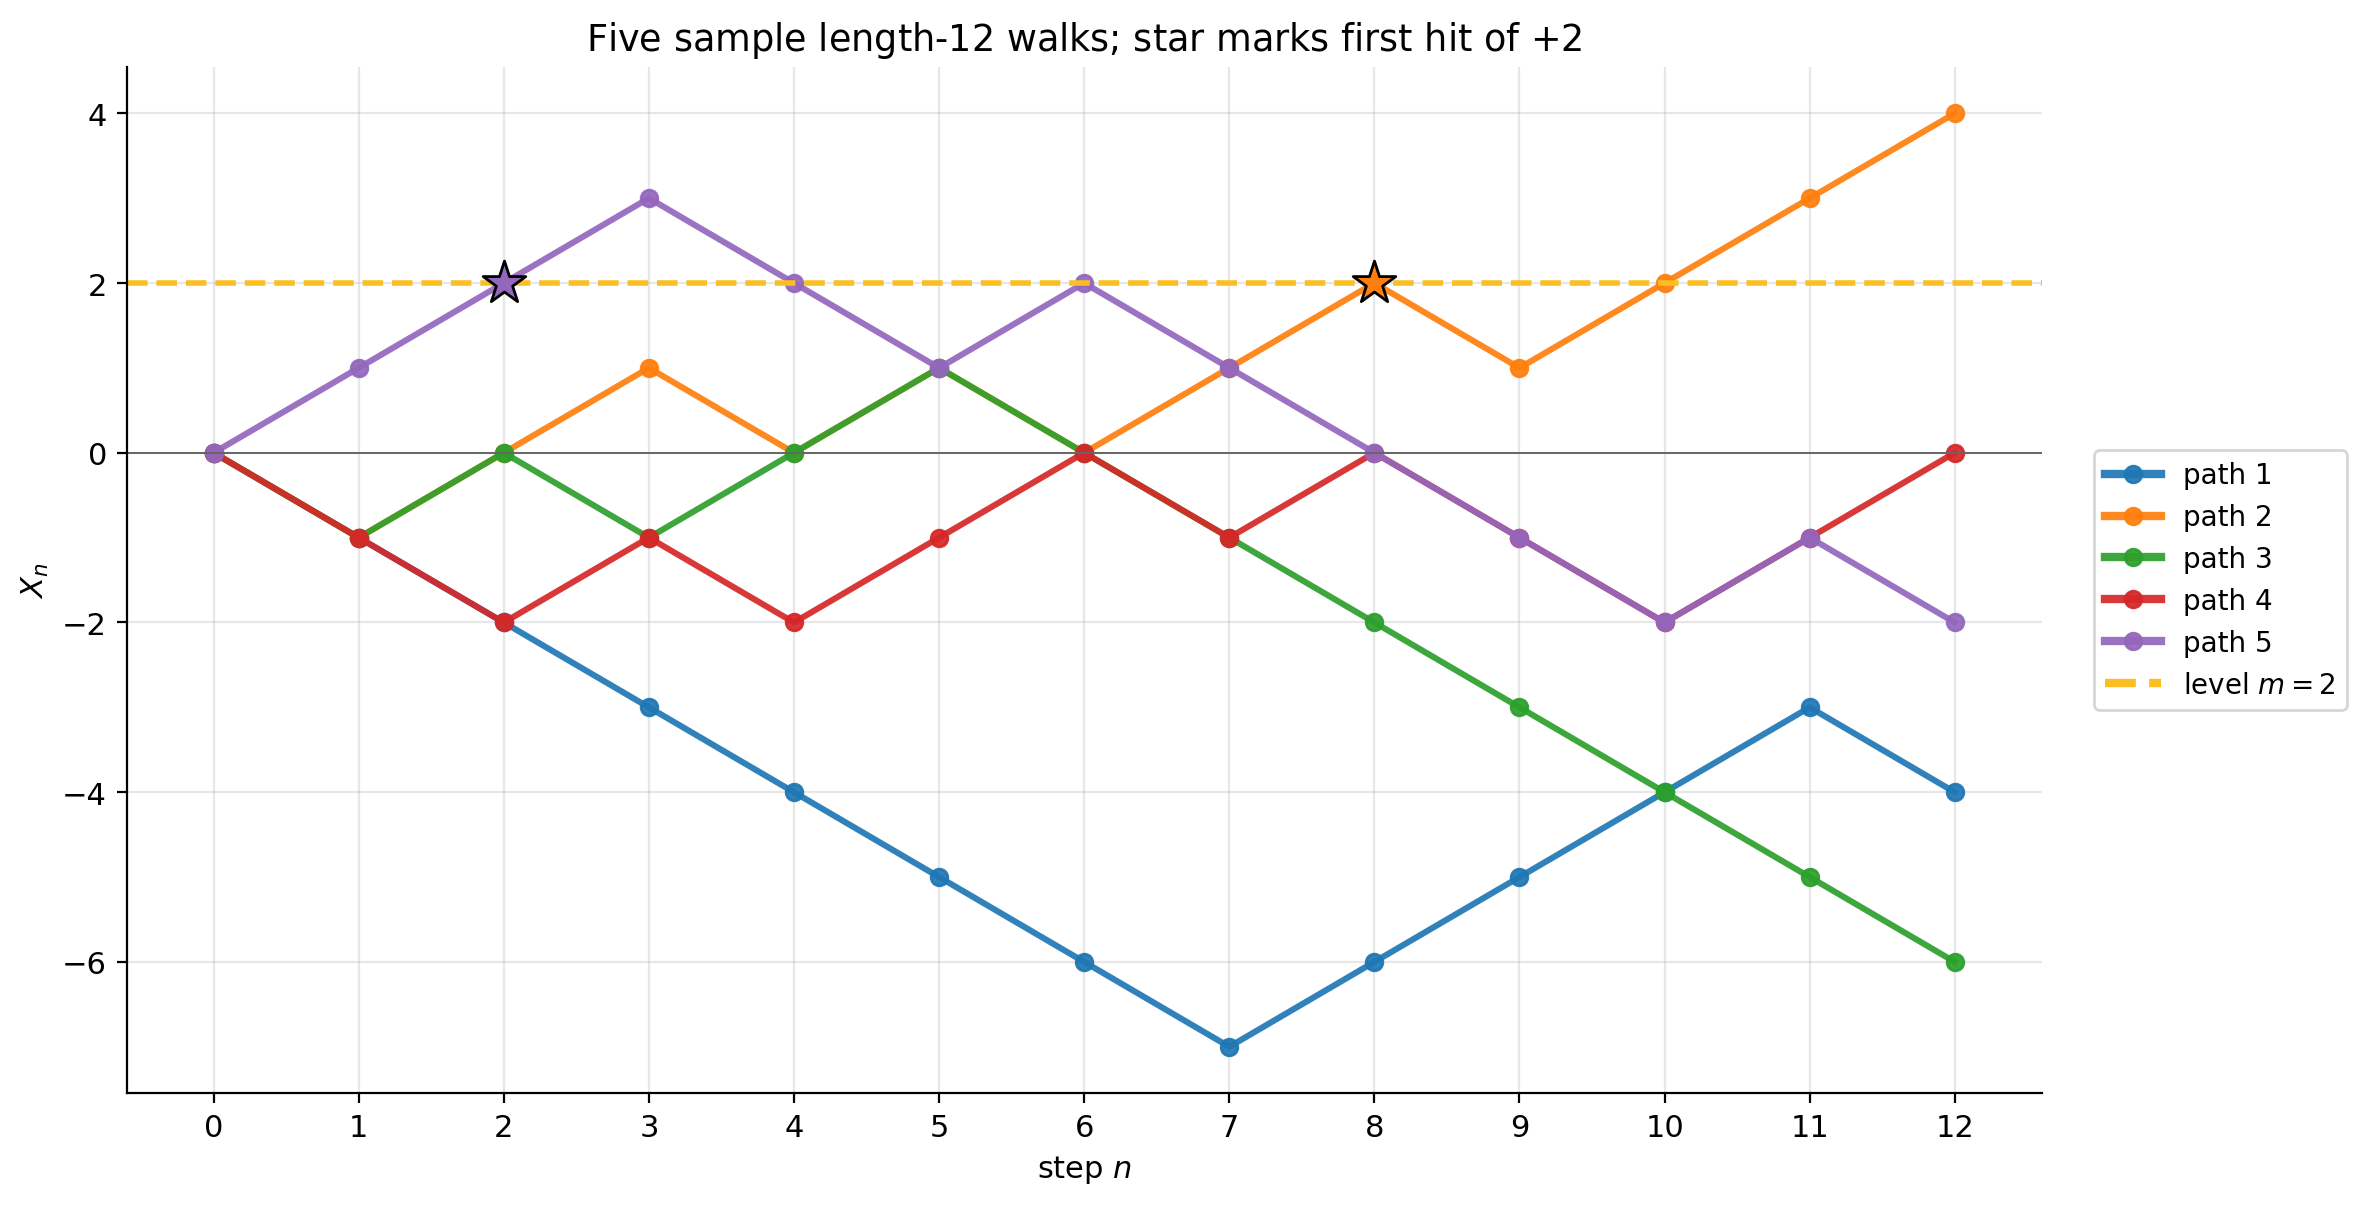
\includegraphics[keepaspectratio]{figures/ch05-tau-sample-paths.png}}
\caption{Five sample symmetric random walks of length 12, with the
first-hit time of \(m = 2\) marked by a star. One path (purple) reaches
\(+2\) very quickly; one (red) never reaches \(+2\) at all in the 12
steps shown.}
\end{figure}

\subsection{5.4.3 Tables}\label{tables-14}

\textbf{Table 5.8.} \(\mathbb P(\tau_m = n)\) for \(m \in \{1, 2, 3\}\)
and \(n \le 10\), with formula \(\frac{m}{n}\binom{n}{(n+m)/2}/2^n\).
Zero entries (wrong parity or \(n < m\)) omitted.

{\def\LTcaptype{none} % do not increment counter
\begin{table}[H]
\centering
\begin{tabular}{|r|r|r|r|}
\toprule
\(n\) & \(m = 1\) & \(m = 2\) & \(m = 3\) \\
\midrule



\(\phantom{0}1\) & \(0.5000\) & & \\
\(\phantom{0}2\) & & \(0.2500\) & \\
\(\phantom{0}3\) & \(0.1250\) & & \(0.1250\) \\
\(\phantom{0}4\) & & \(0.1250\) & \\
\(\phantom{0}5\) & \(0.0625\) & & \(0.0938\) \\
\(\phantom{0}6\) & & \(0.0781\) & \\
\(\phantom{0}7\) & \(0.0391\) & & \(0.0703\) \\
\(\phantom{0}8\) & & \(0.0547\) & \\
\(\phantom{0}9\) & \(0.0273\) & & \(0.0547\) \\
\(10\) & & \(0.0410\) & \\
\bottomrule
\end{tabular}
\end{table}
}

\emph{Blank: \(\mathbb P(\tau_m = n) = 0\) by parity (n and m must agree
mod 2).}

(All entries verified by direct enumeration of \(2^n\) paths and by
formula.)

\subsection{5.4.4 Exercises}\label{exercises-23}

\begin{enumerate}
\def\labelenumi{\arabic{enumi}.}
\tightlist
\item
  Compute \(\mathbb P(\tau_4 = 4)\). \textbf{Answer:}
  \((4/4)\binom{4}{4}/16 = 1/16\). (Only the all-U path UUUU hits \(+4\)
  for the first time at step 4 --- because that's the only way to even
  reach \(+4\) in 4 steps.)
\item
  Compute \(\mathbb P(\tau_4 \le 6)\). \textbf{Answer:}
  \(\mathbb P(\tau_4 = 4) + \mathbb P(\tau_4 = 6) = 1/16 + (4/6) \cdot \binom{6}{5}/64 = 1/16 + 6/(6 \cdot 64) \cdot 4 = 1/16 + 4/64 = 1/16 + 1/16 = 2/16 = 0.125\).
  (Cross-check by enumeration.)
\item
  Argue intuitively why \(\mathbb E[\tau_1] = \infty\). \textbf{Answer:}
  The walk visits each integer infinitely often \emph{eventually}, but
  the \emph{first} visit to \(+1\) can be delayed indefinitely when the
  walk wanders to large negative values --- and the time to wander back
  from \(-N\) to \(+1\) scales like \(N^2\) on average, faster than the
  probability \(\sim 1/\sqrt N\) of getting that deep.
\end{enumerate}

\begin{center}\rule{0.5\linewidth}{0.5pt}\end{center}

\section{\texorpdfstring{§5.5 Joint distribution of
\((M_n, X_n)\)}{§5.5 Joint distribution of (M\_n, X\_n)}}\label{joint-distribution-of-m_n-x_n}

\textbf{Punchline.} The joint distribution of running-max and endpoint
is given by \textbf{one formula}:

\[\boxed{\;\mathbb P(M_n = m,\, X_n = h) \;=\; \mathbb P(X_n = 2m - h) \;-\; \mathbb P(X_n = 2m - h + 2),\;}\]

valid for integers \(m \ge 0\) and \(h \le m\) with \(h\) of the same
parity as \(n\). (The parity constraint on \(m\) --- needed for the path
to actually attain a maximum at level \(m\) --- is encoded automatically
because \(\mathbb P(X_n = 2m - h)\) vanishes by parity whenever it is
inconsistent.)

\textbf{Intuition.}
\(\mathbb P(M_n \ge m, X_n = h) = \mathbb P(X_n = 2m - h)\) from
reflection. Differencing with \(m + 1\):

\(\mathbb P(M_n = m, X_n = h) = \mathbb P(M_n \ge m, X_n = h) - \mathbb P(M_n \ge m+1, X_n = h)\).

The first term reflects to \(X_n = 2m - h\), the second to
\(X_n = 2(m+1) - h = 2m - h + 2\). Subtract.

\subsection{5.5.1 Examples}\label{examples-26}

\textbf{Example 5.5.1 (full joint pmf at \(n = 4\) from the formula).}
Verify each non-zero entry of Table 5.4.

\begin{itemize}
\tightlist
\item
  \((m, h) = (0, -4)\):
  \(\mathbb P(X_4 = 4) - \mathbb P(X_4 = 6) = 1/16 - 0 = 1/16\). Table:
  \(1/16\). ✓
\item
  \((0, -2)\):
  \(\mathbb P(X_4 = 2) - \mathbb P(X_4 = 4) = 4/16 - 1/16 = 3/16\).
  Table: \(3/16\). ✓
\item
  \((0, 0)\):
  \(\mathbb P(X_4 = 0) - \mathbb P(X_4 = 2) = 6/16 - 4/16 = 2/16\).
  Table: \(2/16\). ✓
\item
  \((1, -2)\): \(\mathbb P(X_4 = 4) - \mathbb P(X_4 = 6) = 1/16\).
  Table: \(1/16\). ✓
\item
  \((1, 0)\): \(\mathbb P(X_4 = 2) - \mathbb P(X_4 = 4) = 3/16\). Table:
  \(3/16\). ✓
\item
  \((2, 0)\): \(\mathbb P(X_4 = 4) - \mathbb P(X_4 = 6) = 1/16\). Table:
  \(1/16\). ✓
\item
  \((2, 2)\): \(\mathbb P(X_4 = 2) - \mathbb P(X_4 = 4) = 3/16\). Table:
  \(3/16\). ✓
\item
  \((3, 2)\): \(\mathbb P(X_4 = 4) - \mathbb P(X_4 = 6) = 1/16\). Table:
  \(1/16\). ✓
\item
  \((4, 4)\): \(\mathbb P(X_4 = 4) - \mathbb P(X_4 = 6) = 1/16\). Table:
  \(1/16\). ✓
\end{itemize}

Nine entries, all confirmed. The formula reproduces the table perfectly.

\textbf{Example 5.5.2 (spot-check at \(n = 6\)).} Three cells from the
heatmap below.

\begin{itemize}
\tightlist
\item
  \((m, h) = (3, 1)\):
  \(\mathbb P(X_6 = 5) - \mathbb P(X_6 = 7) = 6/64 - 0/64 = 6/64\).
\item
  \((m, h) = (2, 0)\):
  \(\mathbb P(X_6 = 4) - \mathbb P(X_6 = 6) = 6/64 - 1/64 = 5/64\).
\item
  \((m, h) = (1, 1)\):
  \(\mathbb P(X_6 = 1) - \mathbb P(X_6 = 3) = 0 - 0\) --- wait, \(X_6\)
  is even (parity), so \(\mathbb P(X_6 = 1) = 0\). The formula gives 0,
  which is consistent with the parity constraint: if \(n = 6\) is even,
  \(h\) must be even, but \(h = 1\) is odd, so this entry isn't in the
  support.
\end{itemize}

The parity check is built into the formula automatically ---
non-existent cells become \(0 - 0\).

\textbf{Example 5.5.3 (\(\mathbb E[M_4]\) from the marginal).} The
marginal \(\mathbb P(M_4 = m)\) is got by summing the joint over \(h\):

\begin{itemize}
\tightlist
\item
  \(\mathbb P(M_4 = 0) = 1/16 + 3/16 + 2/16 = 6/16\).
\item
  \(\mathbb P(M_4 = 1) = 1/16 + 3/16 = 4/16\).
\item
  \(\mathbb P(M_4 = 2) = 1/16 + 3/16 = 4/16\).
\item
  \(\mathbb P(M_4 = 3) = 1/16\).
\item
  \(\mathbb P(M_4 = 4) = 1/16\).
\end{itemize}

\(\mathbb E[M_4] = 0 \cdot 6/16 + 1 \cdot 4/16 + 2 \cdot 4/16 + 3 \cdot 1/16 + 4 \cdot 1/16 = (4 + 8 + 3 + 4)/16 = 19/16 = 1.1875\).

Note \(\mathbb E[X_4] = 0\) but \(\mathbb E[M_4] > 0\) --- the running
maximum is biased upward, as expected.

\textbf{Example 5.5.4 (\(\mathbb E[M_n]\) scaling).} From the asymptotic
relation \(\mathbb P(M_n \ge a\sqrt n) \to 2(1 - \Phi(a))\), one can
show

\[\mathbb E[M_n] \;\sim\; \sqrt{2n/\pi}.\]

At \(n = 4\): prediction \(\sqrt{8/\pi} \approx 1.596\). Actual:
\(1.1875\). Off by \(\sim 30\%\) --- small \(n\) corrections matter. At
\(n = 100\) the agreement is excellent.

\begin{figure}
\centering
\pandocbounded{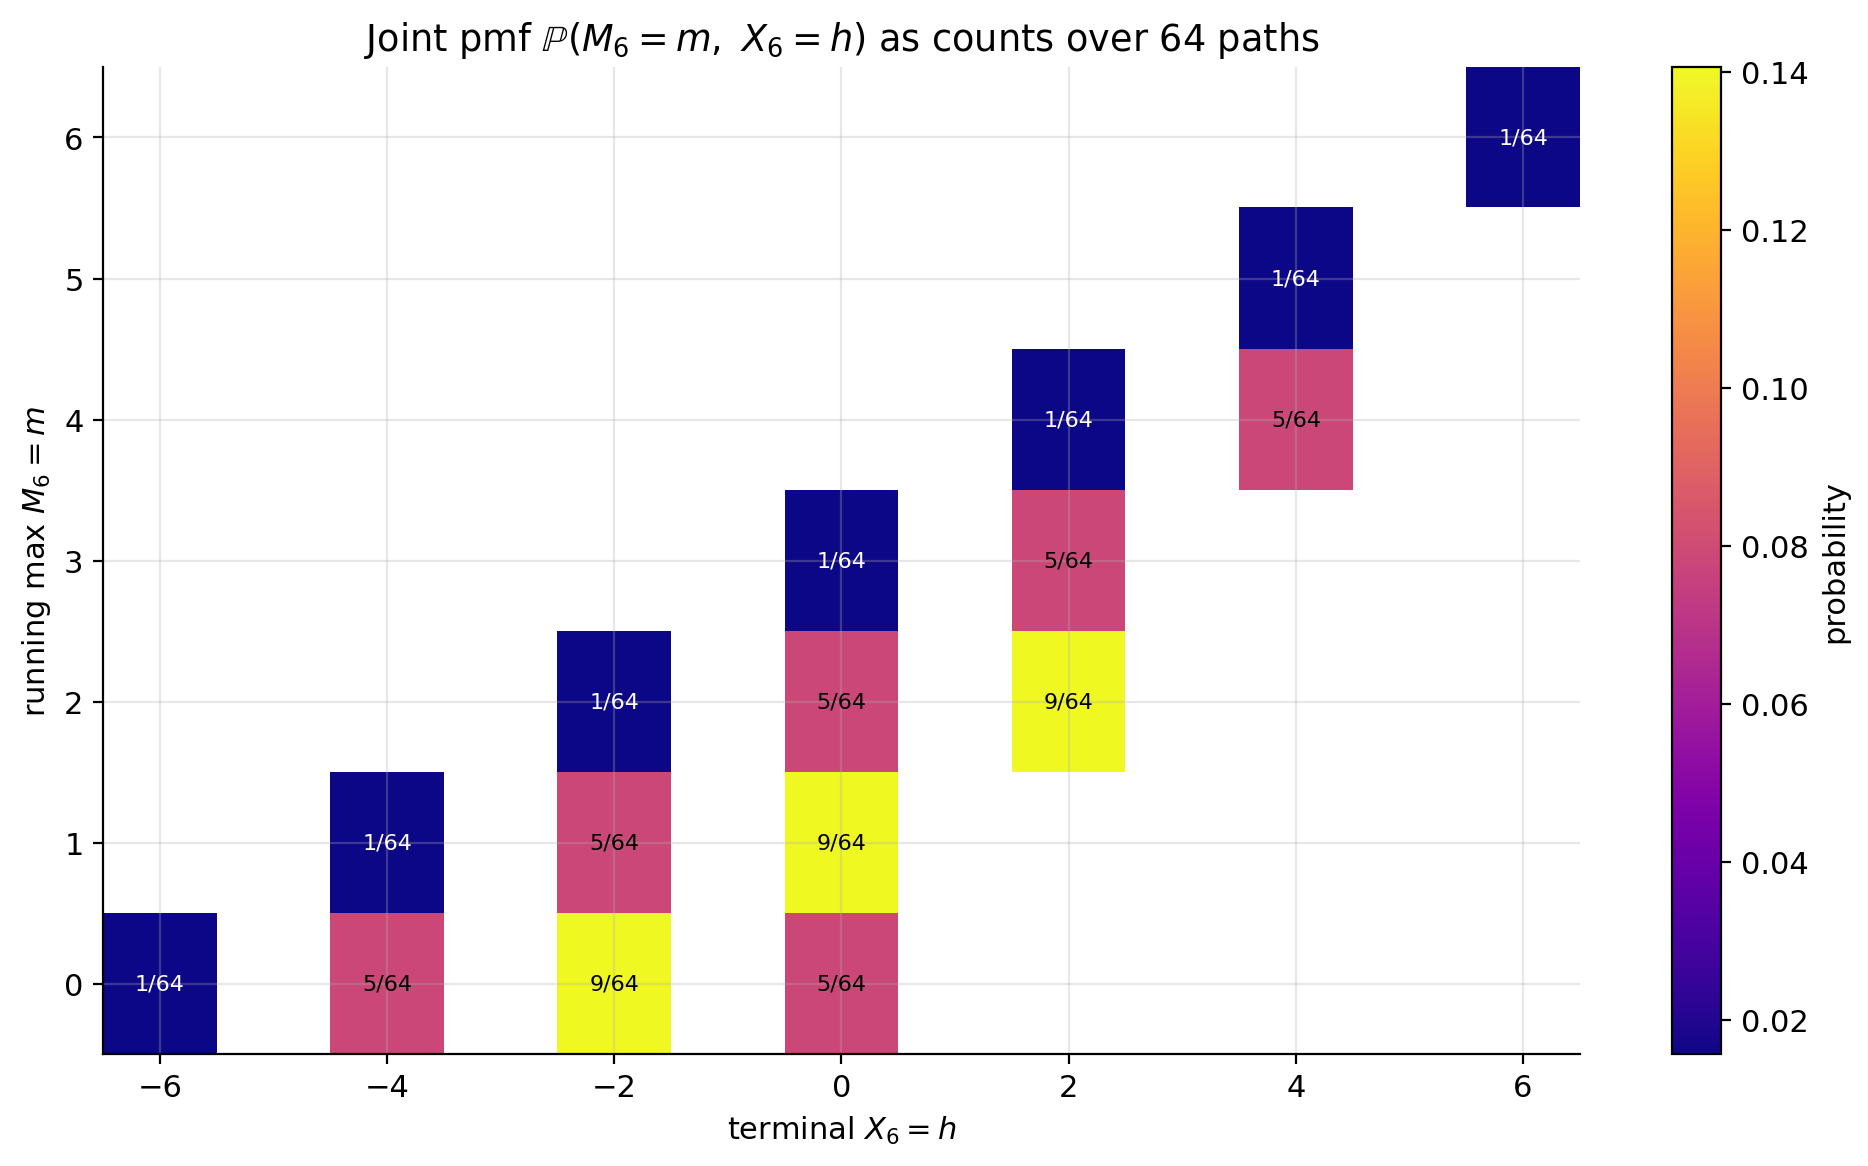
\includegraphics[keepaspectratio]{figures/ch05-joint-heatmap.png}}
\caption{Heatmap of the joint pmf \(\mathbb P(M_6 = m, X_6 = h)\) over
all \(64\) length-6 paths. Empty cells (different parity, or \(h > m\))
are masked. The ``diagonal'' \(h = m\) holds many of the
high-probability cells: when the walk ends at its peak, that peak is
exactly the endpoint.}
\end{figure}

\begin{figure}
\centering
\pandocbounded{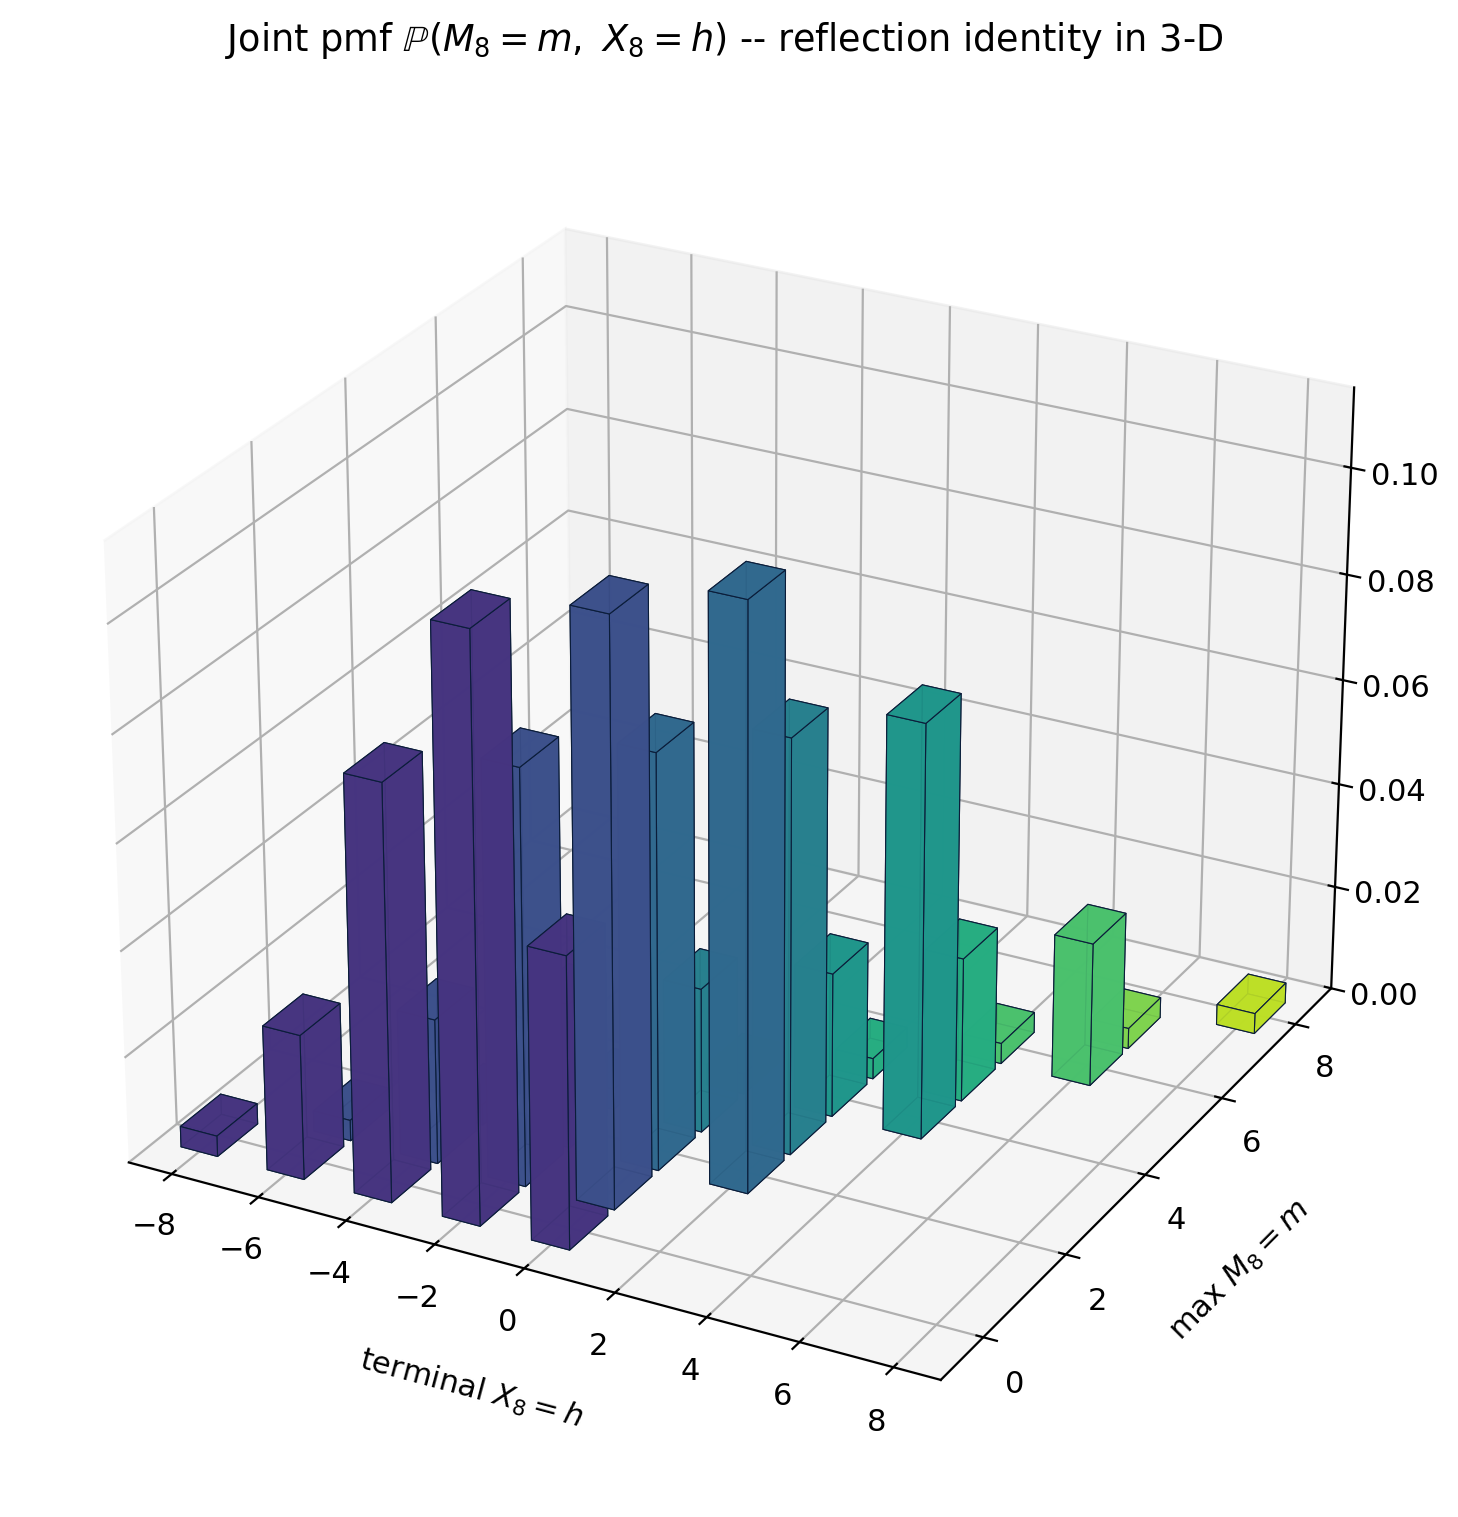
\includegraphics[keepaspectratio]{figures/ch05-joint-bar-3d.png}}
\caption{Three-dimensional bar chart of \(\mathbb P(M_8 = m, X_8 = h)\).
Bars are coloured by \(m\). The constraint \(h \le m\) shows up as the
truncation in the \((h, m)\) plane.}
\end{figure}

\subsection{5.5.2 Tables}\label{tables-15}

\textbf{Table 5.9.} Joint pmf at \(n = 4\): formula evaluation vs
enumerated counts. The formula is
\(\mathbb P(M_n = m, X_n = h) = \mathbb P(X_n = 2m - h) - \mathbb P(X_n = 2m - h + 2)\).
The ``diff'' column below shows the two raw
\(\mathbb P(X_4=\cdot)\cdot 16\) counts being subtracted.

{\def\LTcaptype{none} % do not increment counter
\begin{table}[H]
\centering
\begin{tabular}{|l|l|r|r|}
\toprule
\((m, h)\) & diff \(\times 16\) & count & prob. \\
\midrule



\((0, -4)\) & \(1 - 0\) & \(1\) & \(1/16\) \\
\((0, -2)\) & \(4 - 1\) & \(3\) & \(3/16\) \\
\((0, 0)\) & \(6 - 4\) & \(2\) & \(2/16\) \\
\((1, -2)\) & \(1 - 0\) & \(1\) & \(1/16\) \\
\((1, 0)\) & \(4 - 1\) & \(3\) & \(3/16\) \\
\((2, 0)\) & \(1 - 0\) & \(1\) & \(1/16\) \\
\((2, 2)\) & \(4 - 1\) & \(3\) & \(3/16\) \\
\((3, 2)\) & \(1 - 0\) & \(1\) & \(1/16\) \\
\((4, 4)\) & \(1 - 0\) & \(1\) & \(1/16\) \\
\bottomrule
\end{tabular}
\end{table}
}

\emph{Legend:} ``diff \(\times 16\)'' is the unnormalised count
difference
\(\mathbb P(X_n = 2m - h)\cdot 16 - \mathbb P(X_n = 2m - h + 2)\cdot 16\).

Every formula entry matches the count. (Counts are unnormalized, out of
16.)

\begin{center}\rule{0.5\linewidth}{0.5pt}\end{center}

\section{§5.6 Pricing knock-in / knock-out barrier options on a binomial
tree}\label{pricing-knock-in-knock-out-barrier-options-on-a-binomial-tree}

\textbf{Punchline.} A barrier option's payoff depends on whether the
price ever crossed \(L\). The reflection principle turns ``ever crossed
\(L\)'' into a \emph{count of endpoint paths}. \textbf{Same complexity
as a vanilla European option.}

\textbf{In--out parity.} If \(V^{\text{KI}}\) is a knock-in option and
\(V^{\text{KO}}\) is its knock-out twin (same strike, same type), and
\(V^{\text{vanilla}}\) is the corresponding vanilla:

\[\boxed{\;V^{\text{KI}} + V^{\text{KO}} \;=\; V^{\text{vanilla}}.\;}\]

Either the path crosses or it doesn't --- one of the two options pays
exactly what the vanilla pays. So pricing either one prices both.

\subsection{\texorpdfstring{5.6.1 Worked example: \(S_0 = 4\),
\(u = 2\), \(d = 1/2\), \(r = 1/4\), \(n = 3\), \(K = 5\), \(L = 16\),
up-and-in
call}{5.6.1 Worked example: S\_0 = 4, u = 2, d = 1/2, r = 1/4, n = 3, K = 5, L = 16, up-and-in call}}\label{worked-example-s_0-4-u-2-d-12-r-14-n-3-k-5-l-16-up-and-in-call}

Risk-neutral probability:
\(\tilde p = ((1+r) - d)/(u - d) = (1.25 - 0.5)/1.5 = 0.5\).
(Convenient!) Discount factor: \(1/(1+r)^3 = 1/(1.25)^3 = 0.512\).

Enumerate all 8 paths. The barrier \(L = 16\) on the stock corresponds
to the level \(m = 2\) on the \(X\) walk
(\(S_n \ge 16 \Leftrightarrow X_n \ge 2 \Leftrightarrow\) visited level
2).

{\def\LTcaptype{none} % do not increment counter
\begin{table}[H]
\centering
\begin{tabular}{|l|r|r|r|r|c|r|r|}
\toprule
Path & \(S_1\) & \(S_2\) & \(S_3\) & \(M^S_3\) & hit & payoff & RN
prob \\
\midrule



UUU & \(8\) & \(16\) & \(32\) & \(32\) & ✓ & \(27\) & \(0.125\) \\
UUD & \(8\) & \(16\) & \(8\) & \(16\) & ✓ & \(3\) & \(0.125\) \\
UDU & \(8\) & \(4\) & \(8\) & \(8\) & ✗ & \(3\) & \(0.125\) \\
UDD & \(8\) & \(4\) & \(2\) & \(8\) & ✗ & \(0\) & \(0.125\) \\
DUU & \(2\) & \(4\) & \(8\) & \(8\) & ✗ & \(3\) & \(0.125\) \\
DUD & \(2\) & \(4\) & \(2\) & \(4\) & ✗ & \(0\) & \(0.125\) \\
DDU & \(2\) & \(1\) & \(2\) & \(4\) & ✗ & \(0\) & \(0.125\) \\
DDD & \(2\) & \(1\) & \(0.5\) & \(4\) & ✗ & \(0\) & \(0.125\) \\
\bottomrule
\end{tabular}
\end{table}
}

\emph{Legend:} ``hit'' = path touched \(L = 16\); ``payoff''
\(= \max(S_3 - K, 0)\).

Up-and-in call price =
\(0.512 \cdot 0.125 \cdot (27 + 3) = 0.512 \cdot 30/8 = 0.512 \cdot 3.75 = \mathbf{1.9200}\).

\textbf{Example 5.6.1 (full vanilla price).} Sum payoffs over \emph{all}
paths:
\(0.512 \cdot 0.125 \cdot (27 + 3 + 3 + 0 + 3 + 0 + 0 + 0) = 0.512 \cdot 36/8 = 0.512 \cdot 4.5 = \mathbf{2.3040}\).

\textbf{Example 5.6.2 (knock-out by parity).}
\(V^{\text{KO}} = V^{\text{vanilla}} - V^{\text{KI}} = 2.3040 - 1.9200 = \mathbf{0.3840}\).

Cross-check by direct sum over the 5 non-hitting paths:
\(0.512 \cdot 0.125 \cdot (3 + 0 + 3 + 0 + 0) = 0.512 \cdot 6/8 = 0.384\).
✓

\subsection{\texorpdfstring{5.6.2 Worked example: realistic
\(S_0 = 100\), \(u = 1.10\), \(d = 0.90\), \(r = 0\), \(n = 4\),
\(K = 100\), \(L = 120\), up-and-in
call}{5.6.2 Worked example: realistic S\_0 = 100, u = 1.10, d = 0.90, r = 0, n = 4, K = 100, L = 120, up-and-in call}}\label{worked-example-realistic-s_0-100-u-1.10-d-0.90-r-0-n-4-k-100-l-120-up-and-in-call}

Note \(u \cdot d = 0.99 \ne 1\) --- the log walk is \emph{not} perfectly
symmetric. But we can still price by direct enumeration; reflection just
isn't the most efficient counting tool.

Risk-neutral: \(\tilde p = (1 - 0.90)/(1.10 - 0.90) = 0.10/0.20 = 0.5\).
Discount: \(1/(1.0)^4 = 1.0\) since \(r = 0\). So each path's
probability is \(0.5^4 = 1/16\).

Enumerating (computer):

{\def\LTcaptype{none} % do not increment counter
\begin{table}[H]
\centering
\begin{tabular}{|l|r|r|r|r|r|c|r|}
\toprule
Path & \(S_1\) & \(S_2\) & \(S_3\) & \(S_4\) & \(M^S_4\) & hit & \((S_4-100)^+\) \\
\midrule



UUUU & \(110.00\) & \(121.00\) & \(133.10\) & \(146.41\) & \(146.41\) &
✓ & \(46.41\) \\
UUUD & \(110.00\) & \(121.00\) & \(133.10\) & \(119.79\) & \(133.10\) &
✓ & \(19.79\) \\
UUDU & \(110.00\) & \(121.00\) & \(108.90\) & \(119.79\) & \(121.00\) &
✓ & \(19.79\) \\
UUDD & \(110.00\) & \(121.00\) & \(108.90\) & \(98.01\) & \(121.00\) & ✓
& \(0.00\) \\
(others) & & & & & \(< 120\) & ✗ & various \\
\bottomrule
\end{tabular}
\end{table}
}

\emph{Legend:} ``hit'' = hits \(L \ge 120\). The ``others'' row
aggregates the remaining 12 of 16 paths, none of which touch the
barrier.

Up-and-in call price
\(= (1/16) \cdot (46.41 + 19.79 + 19.79 + 0.00) = 86.00/16 = \mathbf{5.3744}\).

Vanilla call price (sum over all 16 paths, computer):
\(\mathbf{7.8481}\).

Knock-out call price by parity: \(7.8481 - 5.3744 = \mathbf{2.4737}\).

\textbf{Example 5.6.3 (cross-check KO directly).} Sum vanilla payoffs
only over paths that did \emph{not} hit \(L = 120\). Those 12 paths
contribute terminal values below 120 (or zero payoff). Direct
enumeration: \(2.4737\). ✓ The in--out parity holds.

\subsection{\texorpdfstring{5.6.3 Worked example: \(n = 6\), \(K = 4\),
\(L = 16\), up-and-in
call}{5.6.3 Worked example: n = 6, K = 4, L = 16, up-and-in call}}\label{worked-example-n-6-k-4-l-16-up-and-in-call}

Larger lattice. Discount: \(1/(1.25)^6 = 0.2621\). RN prob per path:
\(0.5^6 = 1/64\).

Counting paths: out of 64 length-6 paths, 29 hit the barrier \(L = 16\)
(i.e.~their \(X\)-walk reaches level \(m = 2\)).

By computer: vanilla call \(= 3.2440\), up-and-in call \(= 3.2440\),
knock-out call \(= 0.0000\).

\emph{The vanilla and the up-and-in are equal.} Why? Because every path
that ends with \(S_6 > K = 4\) on this lattice has, somewhere along the
way, also reached \(S = 16\). (To get from \(S_0 = 4\) to
\(S_6 = 8, 16, 32, 64, \ldots\) in only 6 steps, the path must have
spent more time at high \(S\) values than low ones, and indeed must have
touched \(S \ge 16\).) An interesting accident of the symmetric lattice.
The knock-\emph{out} is therefore worthless: any ITM-at-expiry path
knocks out.

This degeneracy disappears when we change \(L\) or \(K\) or use a
non-symmetric lattice. Example 5.6.4 illustrates.

\subsection{\texorpdfstring{5.6.4 Sensitivity: up-and-in call price vs
barrier \(L\) (Toy, \(n = 3\),
\(K = 5\))}{5.6.4 Sensitivity: up-and-in call price vs barrier L (Toy, n = 3, K = 5)}}\label{sensitivity-up-and-in-call-price-vs-barrier-l-toy-n-3-k-5}

Holding the rest fixed and varying \(L\):

{\def\LTcaptype{none} % do not increment counter
\begin{table}[H]
\centering
\begin{tabular}{|r|r|r|r|}
\toprule
\(L\) & up-and-in call \(V^{\text{KI}}\) & knock-out call \(V^{\text{KO}}\) & vanilla \(V^{\text{van}}\) \\
\midrule



\(8\) & \(2.3040\) & \(0.0000\) & \(2.3040\) \\
\(16\) & \(1.9200\) & \(0.3840\) & \(2.3040\) \\
\(32\) & \(1.7280\) & \(0.5760\) & \(2.3040\) \\
\bottomrule
\end{tabular}
\end{table}
}

At \(L = 8\) the barrier is below \(K = 5\), so any ITM path has already
crossed \(L\) --- knock-in equals vanilla and knock-out is worthless. As
\(L\) rises, fewer paths trigger the knock-in: \(V^{\text{KI}}\)
decreases monotonically and \(V^{\text{KO}}\) increases monotonically.
The pair sums to \(V^{\text{vanilla}}\) at every \(L\). ✓

\textbf{Example 5.6.4 (sensitivity, see Figure ch05-ki-price-vs-L).}
\(V^{\text{KI}}\) as a step function of \(L\) --- it can only change at
\(L \in \{\) achievable price levels \(\}\). For Toy \(n = 3\) the
achievable levels are \(\{0.5, 1, 2, 4, 8, 16, 32\}\), so
\(V^{\text{KI}}(L)\) is constant on intervals \(L \in (S_i, S_{i+1}]\)
for those \(S_i\).

\subsection{5.6.5 Down-and-in put}\label{down-and-in-put}

\textbf{Example 5.6.5 (\(S_0 = 4\), \(u = 2\), \(d = 1/2\), \(r = 1/4\),
\(n = 4\), \(K = 4\), \(L = 1\), down-and-in put).} Lower barrier
\(L = 1\) corresponds to \(X\)-level \(-2\) (since
\(4 \cdot 2^{-2} = 1\)).

Enumerating: out of 16 paths, those whose minimum touches \(L = 1\) ---
i.e.~whose minimum on the \(X\) walk is \(\le -2\). By the up-down
symmetry of the symmetric walk, the count of paths with
\(\min X \le -2\) equals the count with \(\max X \ge 2\), which is \(6\)
(Example 5.2.4). So \textbf{6 paths} knock in. The discounted
RN-weighted payoff sum: \(V^{\text{DI}} = 0.4032\).

Vanilla put price: \(V^{\text{van}} = 0.4032\). So
\(V^{\text{DI}} = V^{\text{van}}\) exactly, and \(V^{\text{DO}} = 0\).
\emph{Every path that ends ITM on the put side has also touched
\(L = 1\).} (The put is ITM if \(S_4 < 4\), i.e.~\(X_4 < 0\),
i.e.~\(X_4 \in \{-2, -4\}\), both of which require reaching at least \$X
= -2 = \$ the barrier level.)

Knock-out put: worth zero. Same accident as the symmetric up-and-in
above.

\subsection{5.6.6 In-out parity, numerical
check}\label{in-out-parity-numerical-check}

\textbf{Example 5.6.6 (numerical check of parity).} Across the worked
examples:

{\def\LTcaptype{none} % do not increment counter
\begin{table}[H]
\centering
\begin{tabular}{|l|r|r|r|c|}
\toprule
Setup & \(V^{\text{KI}}\) & \(V^{\text{KO}}\) & \(V^{\text{van}}\) & parity \\
\midrule



ST \(n=3, K=5, L=16\) UI call & \(1.9200\) & \(0.3840\) & \(2.3040\) &
✓ \\
RL \(n=4, K=100, L=120\) UI call & \(5.3744\) & \(2.4737\) & \(7.8481\)
& ✓ \\
ST \(n=6, K=4, L=16\) UI call & \(3.2440\) & \(0.0000\) & \(3.2440\) &
✓ \\
ST \(n=4, K=4, L=1\) DI put & \(0.4032\) & \(0.0000\) & \(0.4032\) &
✓ \\
\bottomrule
\end{tabular}
\end{table}
}

\emph{Parity check:} in every row
\(V^{\text{KI}} + V^{\text{KO}} = V^{\text{van}}\) (e.g.~row 1:
\(1.9200 + 0.3840 = 2.3040\); row 2: \(5.3744 + 2.4737 = 7.8481\)).

In every case the parity holds to numerical precision. \emph{That's the
conceptual reason barrier options are tractable: they're ``complementary
halves'' of a vanilla.}

\begin{figure}
\centering
\pandocbounded{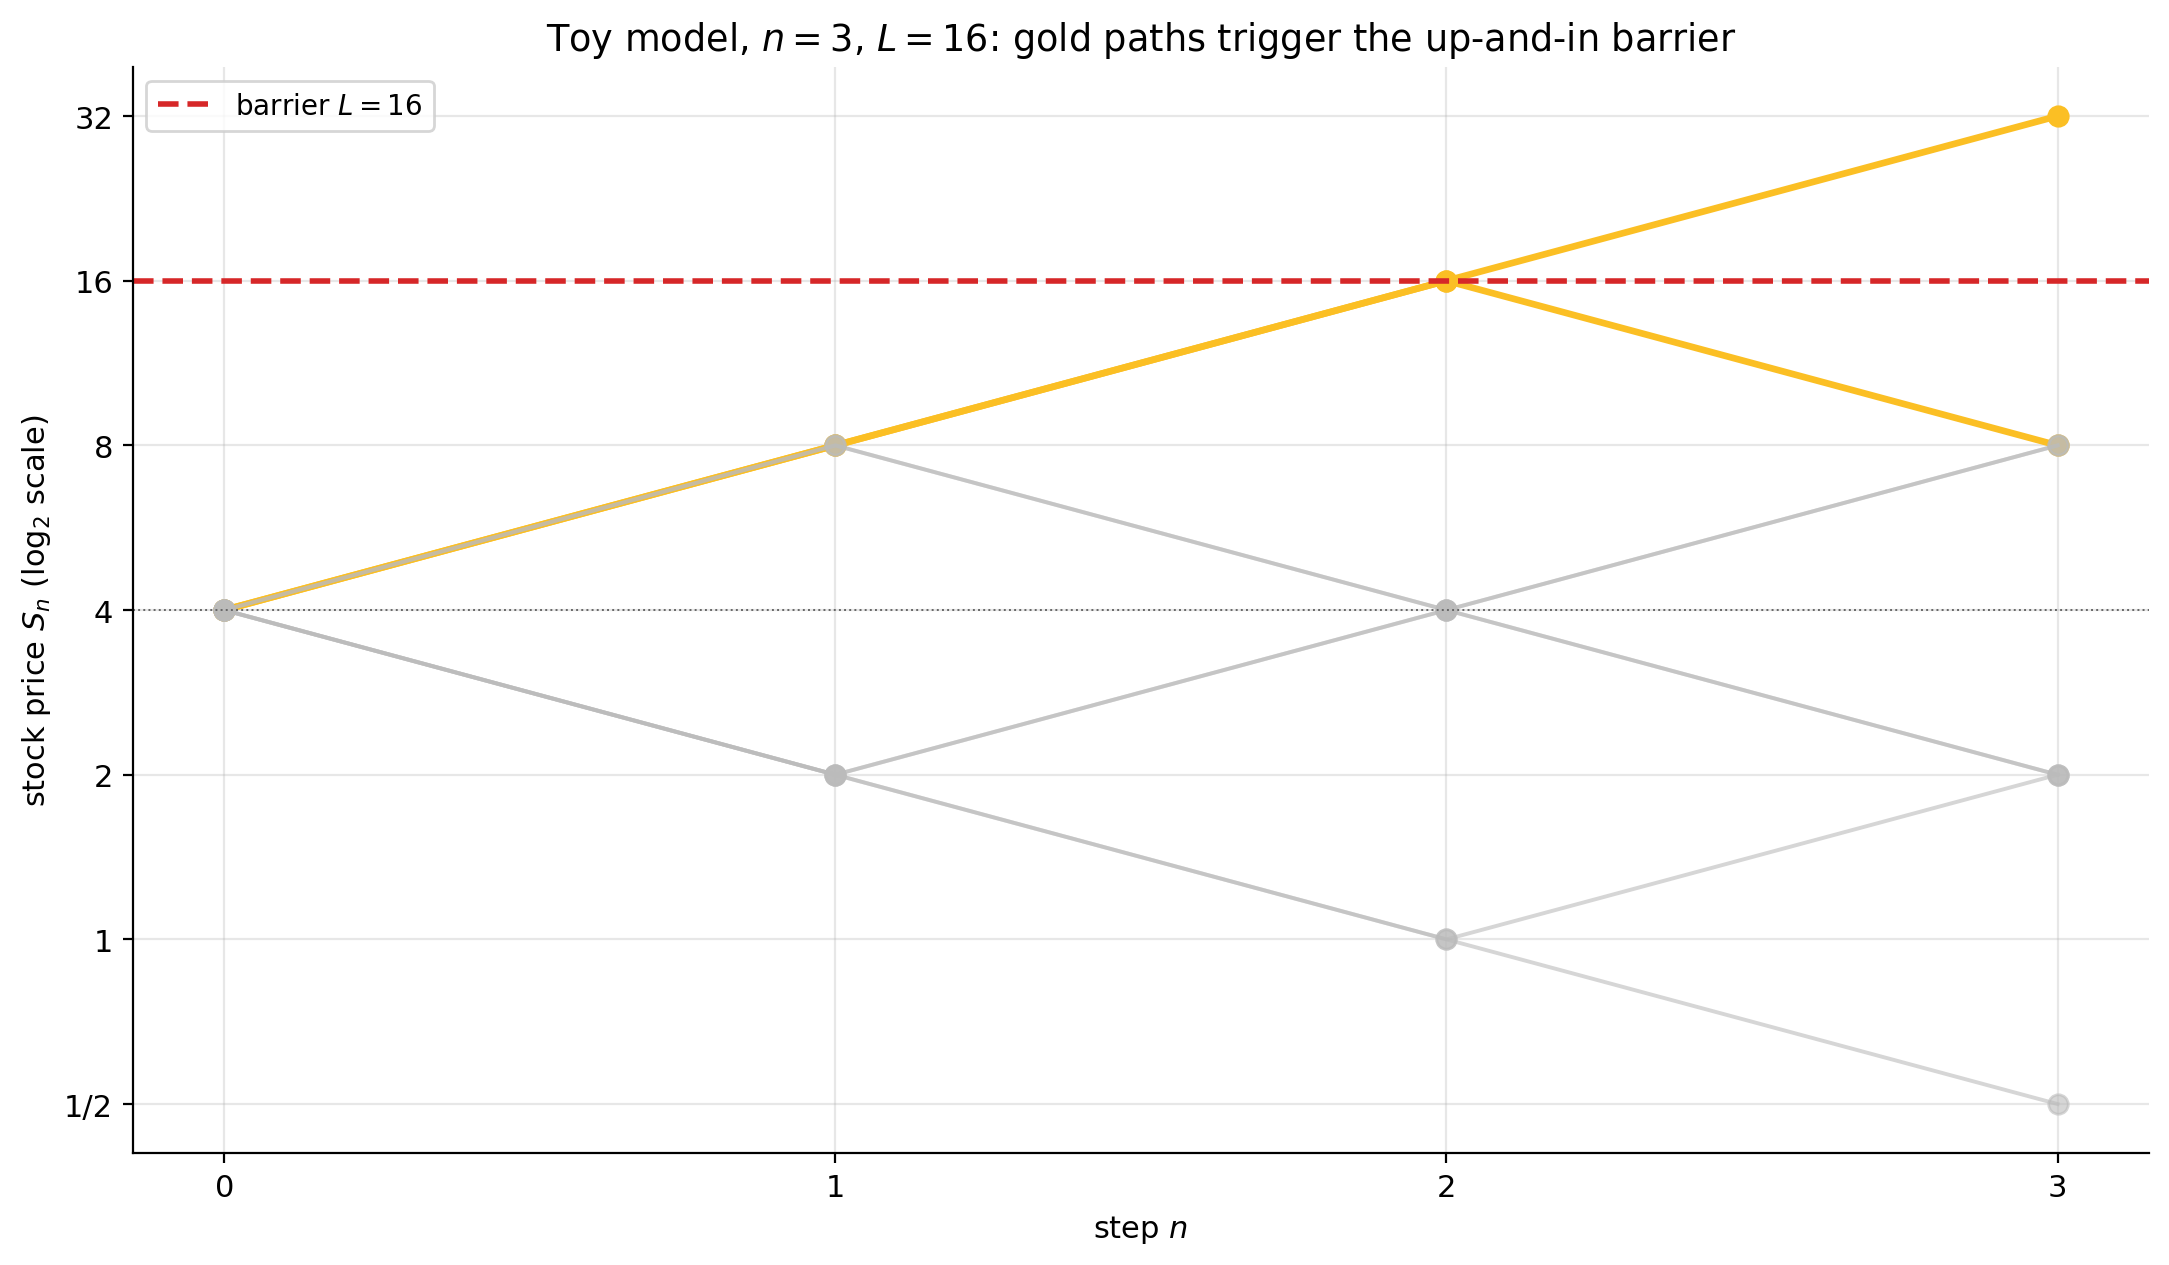
\includegraphics[keepaspectratio]{figures/ch05-knockin-tree-st.png}}
\caption{Toy \(n = 3\), barrier \(L = 16\). Gold paths (UUU, UUD) touch
the barrier and contribute to the up-and-in call; grey paths do not. The
red dashed line is the barrier.}
\end{figure}

\begin{figure}
\centering
\pandocbounded{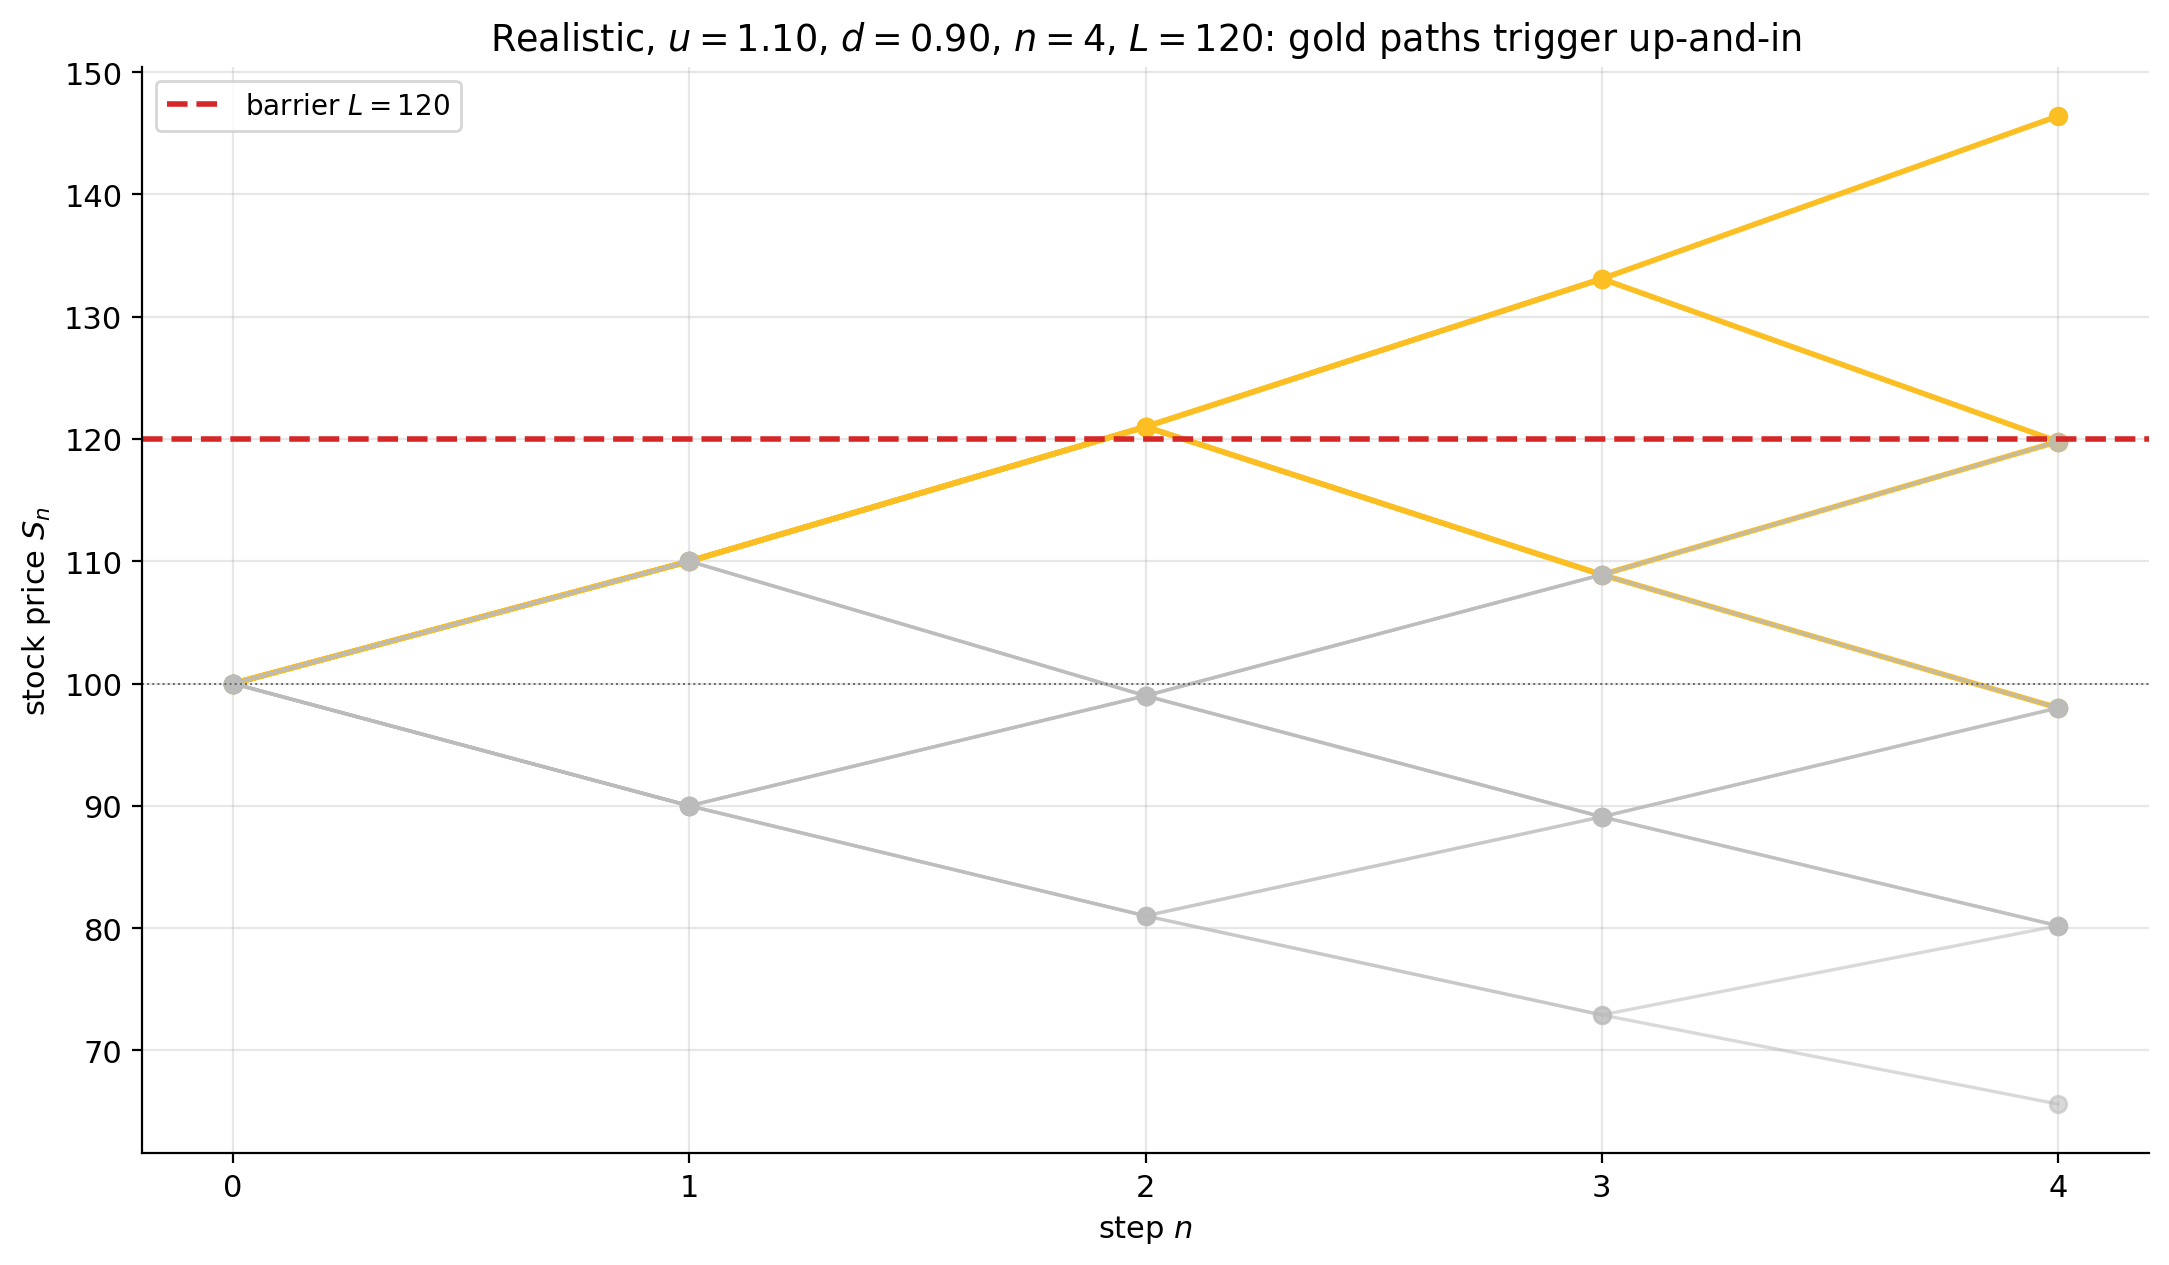
\includegraphics[keepaspectratio]{figures/ch05-knockin-tree-rl.png}}
\caption{Realistic \(u = 1.10, d = 0.90, n = 4\), \(L = 120\). Four
paths (gold) touch the barrier; the other twelve (grey) do not. The
lattice is \emph{not} recombining at integer levels --- each cell's
value depends on the full path of multiplications.}
\end{figure}

\begin{figure}
\centering
\pandocbounded{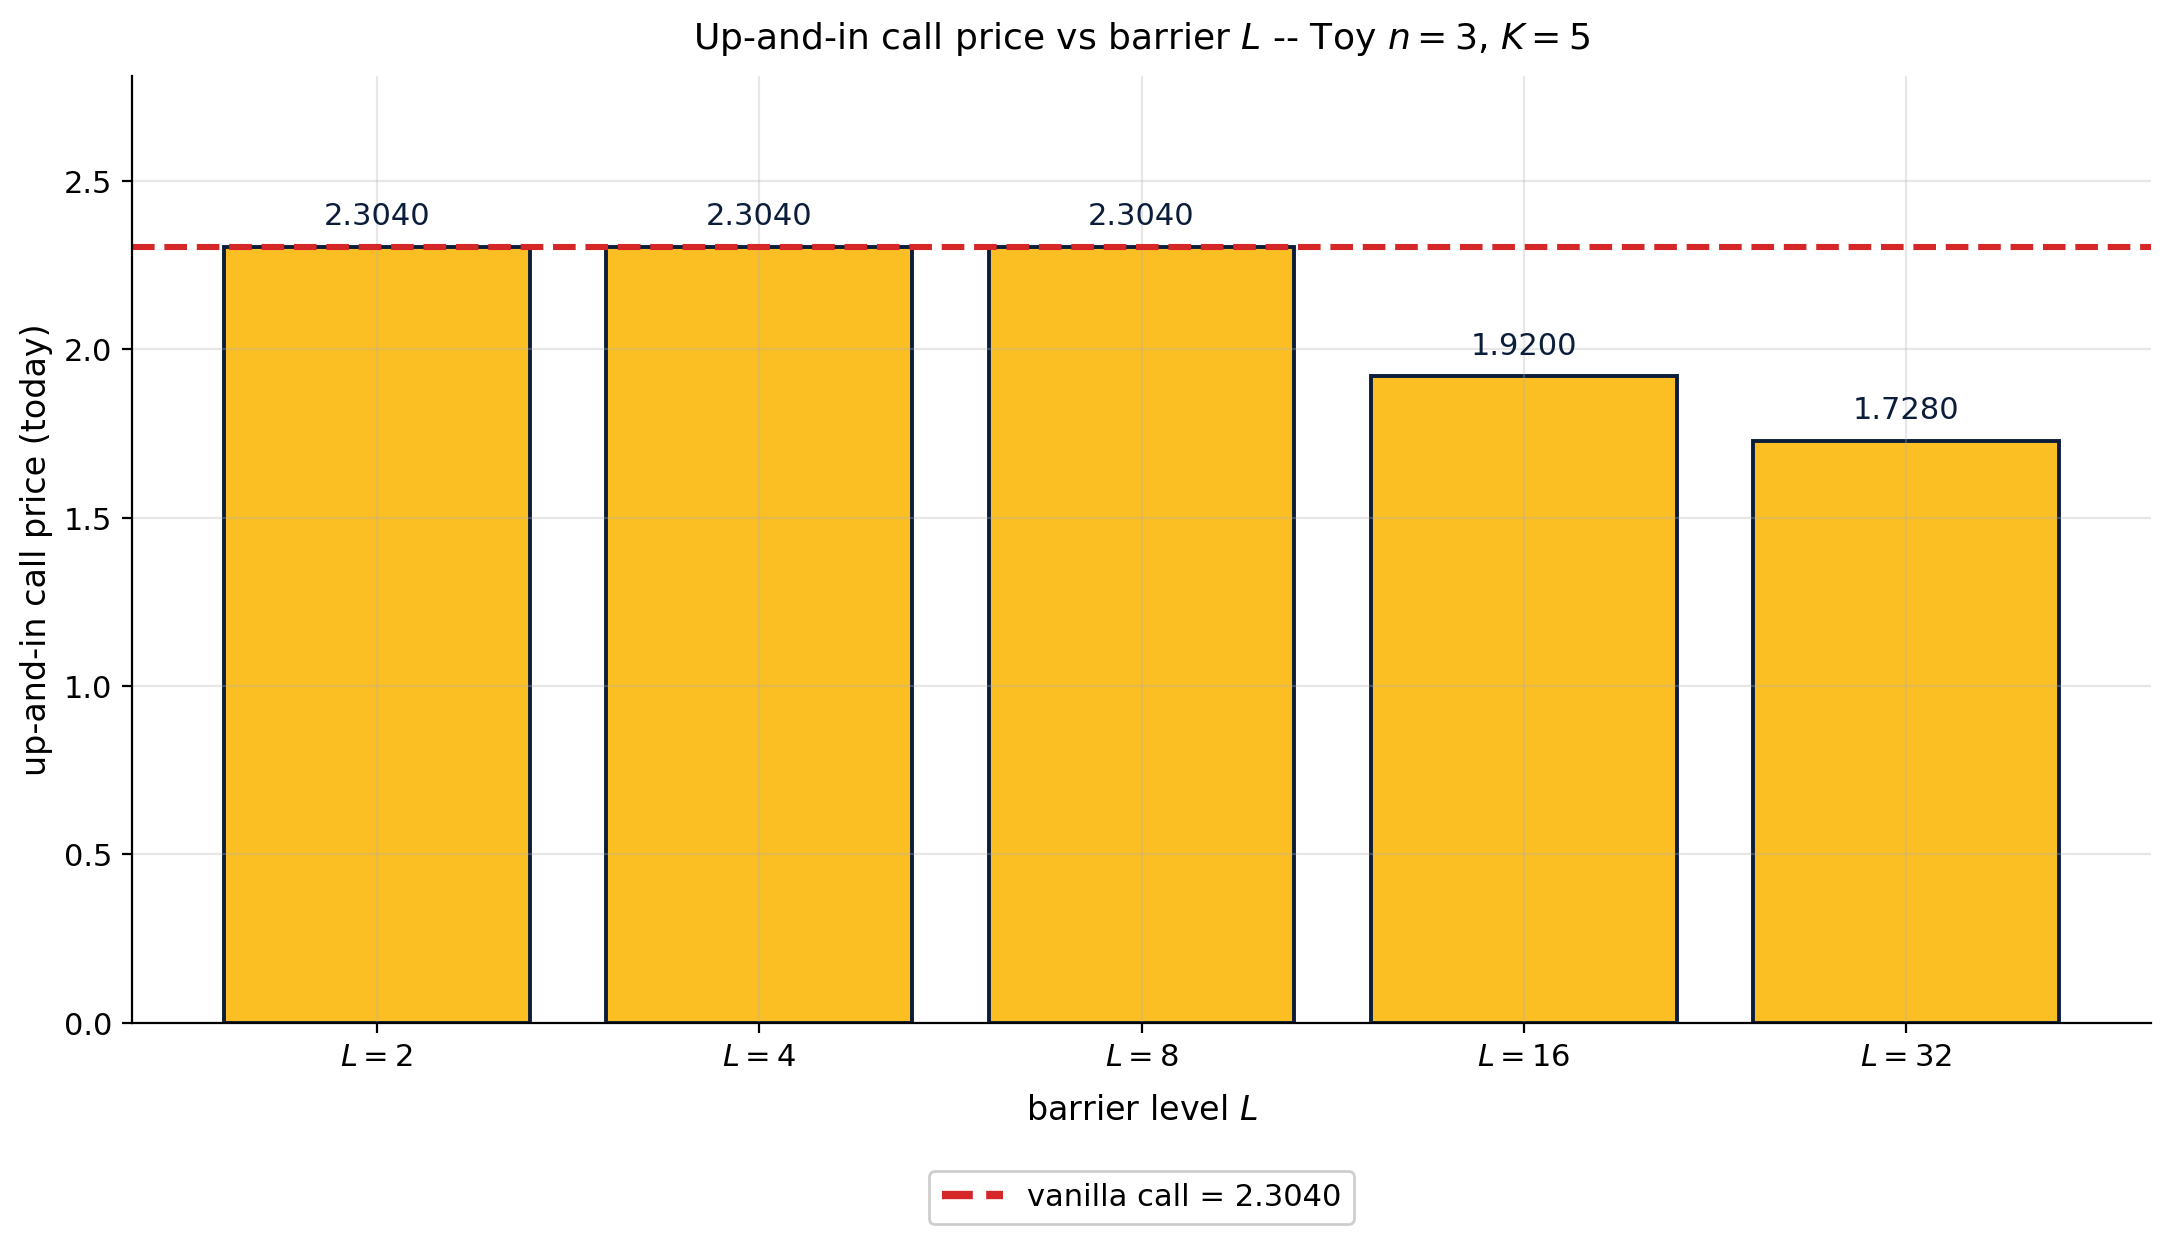
\includegraphics[keepaspectratio]{figures/ch05-ki-price-vs-L.png}}
\caption{Up-and-in call price ( \(n = 3\), \(K = 5\)) as a function of
barrier \(L\). The horizontal red dashed line is the vanilla call price
\(2.3040\). The bars step down as \(L\) rises, with
\(V^{\text{KO}} = V^{\text{vanilla}} - V^{\text{KI}}\) rising in
lockstep.}
\end{figure}

\subsection{5.6.7 Tables}\label{tables-16}

\textbf{Table 5.10.} Toy \(n = 3\), \(K = 5\), \(L = 16\), up-and-in
call --- full path enumeration.

{\def\LTcaptype{none} % do not increment counter
\begin{table}[H]
\centering
\begin{tabular}{|l|r|r|c|r|r|r|}
\toprule
Path & \(S_3\) & \(M^S\) & hit & payoff & RN prob & weighted \\
\midrule



UUU & \(32\) & \(32\) & ✓ & \(27\) & \(1/8\) & \(3.375\) \\
UUD & \(8\) & \(16\) & ✓ & \(3\) & \(1/8\) & \(0.375\) \\
UDU & \(8\) & \(8\) & ✗ & \(3\) & \(1/8\) & \(0.000\) \\
UDD & \(2\) & \(8\) & ✗ & \(0\) & \(1/8\) & \(0.000\) \\
DUU & \(8\) & \(8\) & ✗ & \(3\) & \(1/8\) & \(0.000\) \\
DUD & \(2\) & \(4\) & ✗ & \(0\) & \(1/8\) & \(0.000\) \\
DDU & \(2\) & \(4\) & ✗ & \(0\) & \(1/8\) & \(0.000\) \\
DDD & \(0.5\) & \(4\) & ✗ & \(0\) & \(1/8\) & \(0.000\) \\
\textbf{Sum} & & & & & & \(3.750\) \\
\bottomrule
\end{tabular}
\end{table}
}

\emph{Legend:} ``hit'' = path touched the barrier \(L = 16\);
intermediate \((S_1, S_2)\) values are dropped (see Table 5.5 row 1 for
the full price path). Knock-in (KI) rule: weighted payoff is the path
payoff when ``hit'' = ✓, else \(0\). Rows UDU and DUU have nonzero
payoff but contribute \(0\) to the KI sum (they did not hit).

Discounted: \(V^{\text{KI}} = 0.512 \cdot 3.750 = 1.920\). ✓

\textbf{Table 5.11.} Side-by-side:
\(V^{\text{KI}}, V^{\text{KO}}, V^{\text{van}}\) for several setups.

{\def\LTcaptype{none} % do not increment counter
\begin{table}[H]
\centering
\begin{tabular}{|r|r|r|r|r|r|}
\toprule
\(n\) & \(K\) & \(L\) & \(V^{\text{KI}}\) & \(V^{\text{KO}}\) & \(V^{\text{van}}\) \\
\midrule



\(3\) & \(5\) & \(8\) & \(2.3040\) & \(0.0000\) & \(2.3040\) \\
\(3\) & \(5\) & \(16\) & \(1.9200\) & \(0.3840\) & \(2.3040\) \\
\(3\) & \(5\) & \(32\) & \(1.7280\) & \(0.5760\) & \(2.3040\) \\
\(6\) & \(4\) & \(16\) & \(3.2440\) & \(0.0000\) & \(3.2440\) \\
\bottomrule
\end{tabular}
\end{table}
}

\subsection{5.6.8 Exercises}\label{exercises-24}

\begin{enumerate}
\def\labelenumi{\arabic{enumi}.}
\tightlist
\item
  In the toy with \(n = 3\), \(K = 5\), what is \(V^{\text{KI}}\) when
  \(L = 64\)? \textbf{Answer:} No path can reach \(S = 64\) in 3 steps
  from \(S_0 = 4\) (max reachable is \(32\)). So \(V^{\text{KI}} = 0\)
  and \(V^{\text{KO}} = V^{\text{vanilla}} = 2.3040\).
\item
  (Down-and-out put.) \(n = 3\), \(K = 5\), \(L = 2\). Enumerate which
  paths get knocked out (any path whose running \(\min S\) touches
  \(L = 2\), i.e.~\(\min X \le -1\)). \textbf{Answer:} UDD
  (\(\min S = 2\)), DUD (\(2\)), DDU (\(1\)), DDD (\(0.5\)), and DUU
  (\(\min S = 2\)). UUD's \(\min S = 4\), UDU's is \(4\), UUU's is \(4\)
  --- none of these touch \(L = 2\). So \textbf{five paths} knock out.
  Set up: vanilla put payoffs are \((K - S_3)^+\); the DI put pays the
  same but only on the five knock-in paths; the DO put pays only on the
  remaining three paths.
\item
  Argue informally why \(V^{\text{KI}}(L)\) is non-increasing in \(L\)
  (for an up-and-in call). \textbf{Answer:} Raising \(L\) shrinks the
  set of qualifying paths (subset relation), so the weighted payoff sum
  cannot increase.
\end{enumerate}

\begin{center}\rule{0.5\linewidth}{0.5pt}\end{center}

\section{§5.7 Lookback options}\label{lookback-options}

\textbf{Punchline.} A lookback call's payoff is \((M^S_n - K)^+\) ---
the largest price ever reached during the option's life, minus the
strike. Pricing reduces to the \emph{marginal} distribution of \(M_n\).

\textbf{Intuition.} Forget the endpoint. The lookback only cares about
the \emph{peak}. So once we have \(\mathbb P(M_n = m)\) --- easily
obtained from §5.5 by summing the joint over \(h\) --- we can compute
the expectation in one step.

\subsection{5.7.1 Decomposition formula}\label{decomposition-formula}

\[V^{\text{lookback}} \;=\; (1+r)^{-n}\sum_{m \ge 0} \tilde{\mathbb P}(M_n = m) \cdot (S_0 u^m - K)^+.\]

Here \(\tilde{\mathbb P}\) is the risk-neutral measure --- for the toy
(\(u = 2, d = 1/2, r = 1/4\)) we have \(\tilde p = 1/2\), so it agrees
with the physical symmetric measure.

\subsection{5.7.2 Examples}\label{examples-27}

\textbf{Example 5.7.1 ( \(n = 3\), \(K = 4\), lookback call).}
Enumerating all 8 paths, computing each path's \(M^S_3\), payoff
\((M^S_3 - 4)^+\), RN-weight \(1/8\), and discount \(0.512\):

{\def\LTcaptype{none} % do not increment counter
\begin{table}[H]
\centering
\begin{tabular}{|l|r|r|r|}
\toprule
Path & \(M^S_3\) & \((M^S_3 - 4)^+\) & RN prob \\
\midrule



UUU & \(32\) & \(28\) & \(1/8\) \\
UUD & \(16\) & \(12\) & \(1/8\) \\
UDU & \(8\) & \(4\) & \(1/8\) \\
UDD & \(8\) & \(4\) & \(1/8\) \\
DUU & \(8\) & \(4\) & \(1/8\) \\
DUD & \(4\) & \(0\) & \(1/8\) \\
DDU & \(4\) & \(0\) & \(1/8\) \\
DDD & \(4\) & \(0\) & \(1/8\) \\
\bottomrule
\end{tabular}
\end{table}
}

Expected payoff: \((28 + 12 + 4 + 4 + 4 + 0 + 0 + 0)/8 = 52/8 = 6.5\).
Discounted: \(V^{\text{lb}} = 0.512 \cdot 6.5 = \mathbf{3.328}\).

\textbf{Example 5.7.2 (floating-strike lookback put).} Payoff:
\(M^S_n - S_n \ge 0\) always. The owner gets the \emph{drawdown from
peak}. For the same \(n = 3\) tree:

{\def\LTcaptype{none} % do not increment counter
\begin{table}[H]
\centering
\begin{tabular}{|l|r|r|r|}
\toprule
Path & \(M^S\) & \(S_3\) & \(M^S - S_3\) \\
\midrule



UUU & \(32\) & \(32\) & \(0\) \\
UUD & \(16\) & \(8\) & \(8\) \\
UDU & \(8\) & \(8\) & \(0\) \\
UDD & \(8\) & \(2\) & \(6\) \\
DUU & \(8\) & \(8\) & \(0\) \\
DUD & \(4\) & \(2\) & \(2\) \\
DDU & \(4\) & \(2\) & \(2\) \\
DDD & \(4\) & \(0.5\) & \(3.5\) \\
\bottomrule
\end{tabular}
\end{table}
}

Expected: \((0 + 8 + 0 + 6 + 0 + 2 + 2 + 3.5)/8 = 21.5/8 = 2.6875\).
Discounted: \(0.512 \cdot 2.6875 = \mathbf{1.3760}\).

\textbf{Example 5.7.3 (realistic \(S_0 = 100\), \(u = 1.10\),
\(d = 0.90\), \(r = 0\), \(n = 4\), \(K = 100\) fixed-strike lookback
call).}

Enumerating all 16 paths (computer), expected payoff \(= 11.85\),
discounted (since \(r=0\)): \(\mathbf{11.85}\). Compared to the
realistic vanilla call price \(7.85\) from §5.6, the lookback is about
50\% more expensive --- it captures the peak, not the endpoint, which is
always weakly larger.

\textbf{Example 5.7.4 (decomposition via \(\mathbb P(M_n = m)\)).} Same
setup, \(n = 3\), \(K = 4\). Reading the marginal \(\mathbb P(M_3 = m)\)
off the \(n=3\) enumeration in §5.2:

\(\mathbb P(M_3 = 0) = 3/8\) (DUD, DDU, DDD).
\(\mathbb P(M_3 = 1) = 3/8\) (UDU, UDD, DUU).
\(\mathbb P(M_3 = 2) = 1/8\) (UUD). \(\mathbb P(M_3 = 3) = 1/8\) (UUU).

Stock-level translation: \(S_0 \cdot u^m = 4 \cdot 2^m\), so the peak
stock \(M^S = 4, 8, 16, 32\) at \(m = 0, 1, 2, 3\).

Decomposition:

\(V^{\text{lb}} = 0.512 \cdot [\,3/8 \cdot (4-4)^+ + 3/8 \cdot (8-4)^+ + 1/8 \cdot (16-4)^+ + 1/8 \cdot (32-4)^+\,]\)
\(\quad = 0.512 \cdot [\,3/8 \cdot 0 + 3/8 \cdot 4 + 1/8 \cdot 12 + 1/8 \cdot 28\,]\)
\(\quad = 0.512 \cdot [\,0 + 1.5 + 1.5 + 3.5\,] = 0.512 \cdot 6.5 = \mathbf{3.328}\).

Same answer as direct enumeration. ✓ The decomposition is the more
efficient route once \(n\) is large.

\begin{figure}
\centering
\pandocbounded{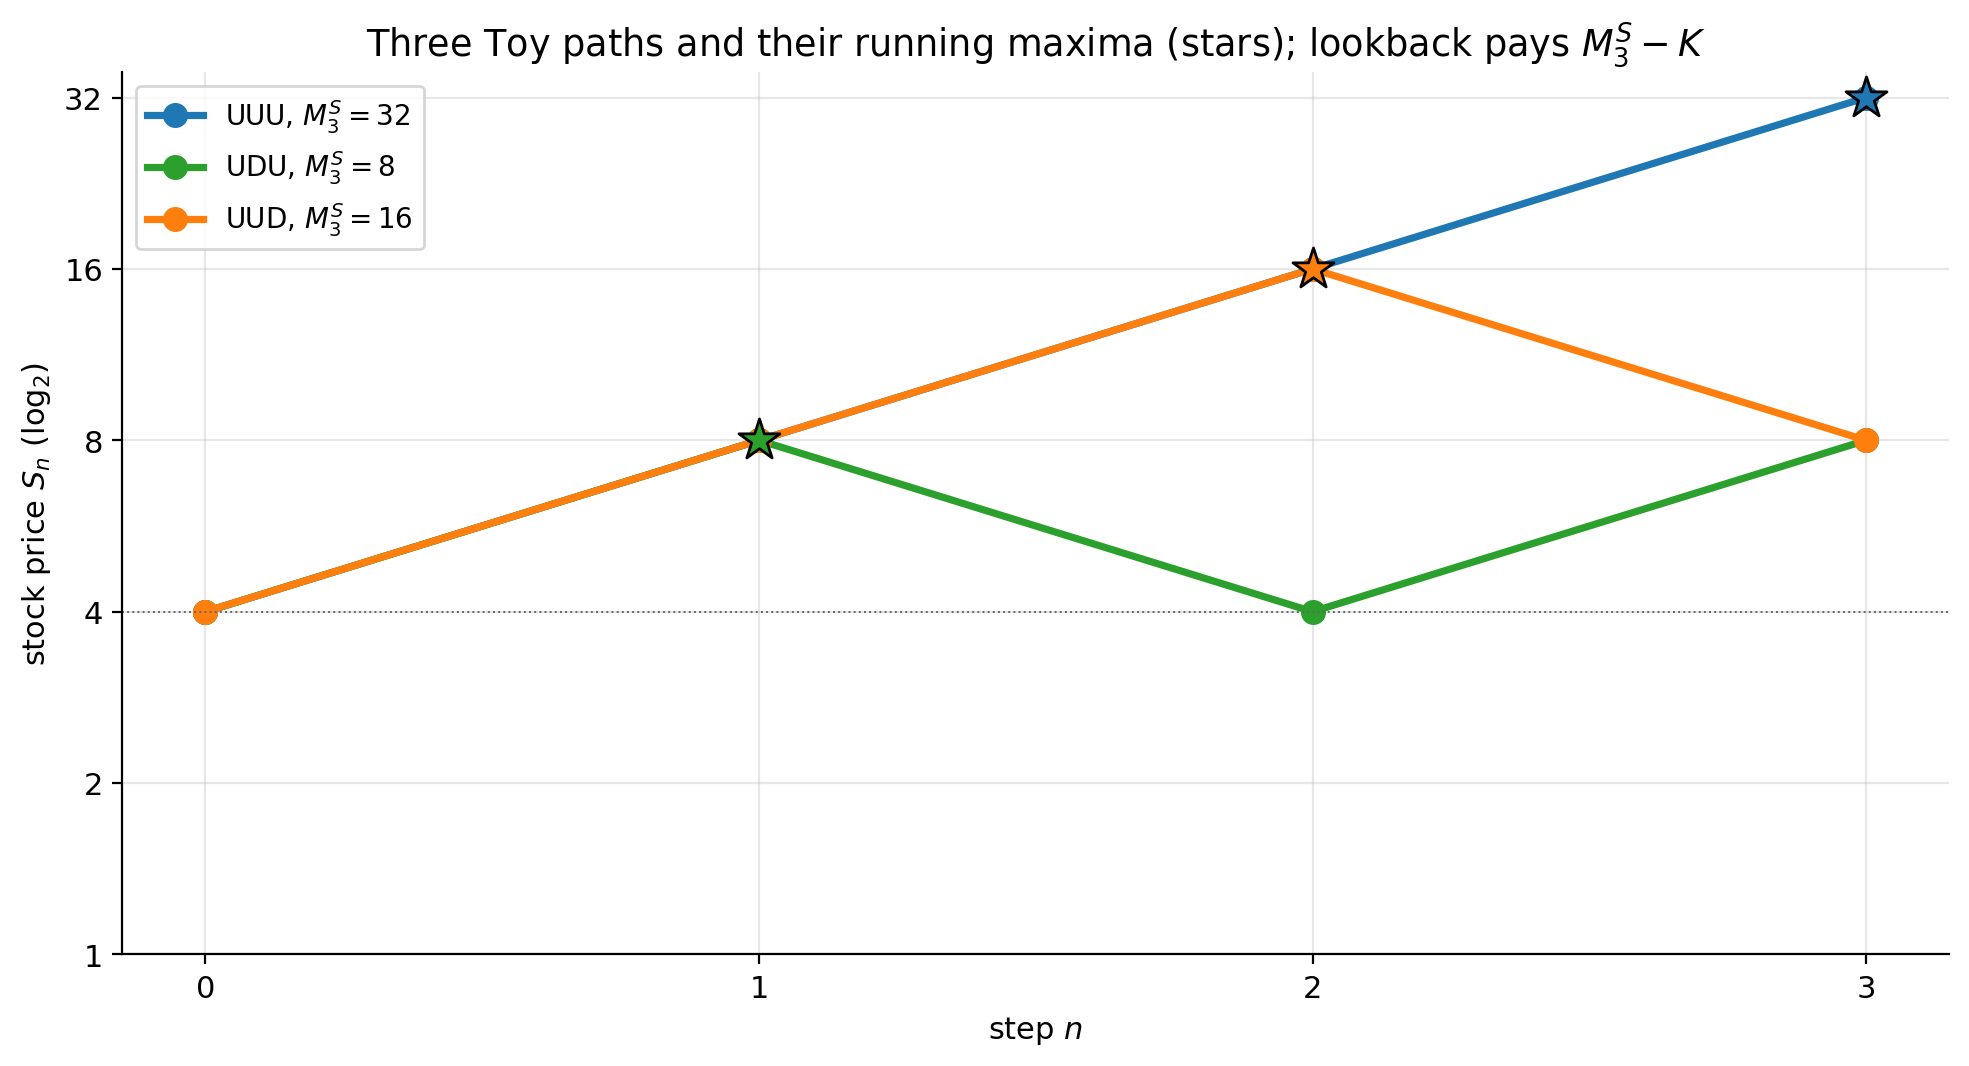
\includegraphics[keepaspectratio]{figures/ch05-lookback-paths.png}}
\caption{Three \(n = 3\) paths (UUU, UUD, UDU) with their running peaks
(stars). The lookback call pays the peak minus \(K\).}
\end{figure}

\subsection{5.7.3 Tables}\label{tables-17}

\textbf{Table 5.12.} Lookback call prices, Toy
(\(u = 2, d = 1/2, r = 1/4\), \(S_0 = 4\)).

{\def\LTcaptype{none} % do not increment counter
\begin{table}[H]
\centering
\begin{tabular}{|r|r|r|r|}
\toprule
\(n\) & \(K = 2\) & \(K = 4\) & \(K = 8\) \\
\midrule



\(2\) & \(3.8400\) & \(2.5600\) & \(1.2800\) \\
\(3\) & \(4.3520\) & \(3.3280\) & \(2.0480\) \\
\(4\) & \(4.7104\) & \(3.8912\) & \(2.8672\) \\
\(5\) & \(4.9971\) & \(4.3418\) & \(3.4406\) \\
\bottomrule
\end{tabular}
\end{table}
}

Each value computed by direct enumeration of \(2^n\) paths and verified
by the decomposition formula. Note prices increase with \(n\) (longer
time = more chances to hit a high peak) and decrease with \(K\) (a
higher strike clips more value).

\subsection{5.7.4 Exercises}\label{exercises-25}

\begin{enumerate}
\def\labelenumi{\arabic{enumi}.}
\tightlist
\item
  Compute the lookback put (floating strike: payoff \(M^S - S_n\)) for
  \(n = 2\). \textbf{Answer:} Enumerate UU \((4 \to 8 \to 16)\), UD, DU,
  DD: \(M^S - S_n = 0, 4, 0, 3\). Expected: \(7/4 = 1.75\). Discounted
  at \(r = 1/4\): \(1.75/(1.25)^2 = 1.12\).
\item
  (Lookback floating-strike call: payoff \(S_n - m^S\) where \(m^S\) is
  the running \emph{min}.) Compute for \(n = 2\). \textbf{Answer:} UU
  has \(S_2 = 16\), \(m^S = 4\), payoff \(12\); UD has \(S_2 = 4\),
  \(m^S = 4\), payoff \(0\); DU has \(S_2 = 4\), \(m^S = 2\), payoff
  \(2\); DD has \(S_2 = 1\), \(m^S = 1\), payoff \(0\). Expected:
  \((12 + 0 + 2 + 0)/4 = 3.5\). Discounted at \(r = 1/4\):
  \(3.5/(1.25)^2 = 3.5/1.5625 = 2.24\).
\item
  Why is the lookback call price weakly larger than the corresponding
  vanilla call price? \textbf{Answer:} Because \(M^S_n \ge S_n\) always,
  so the lookback payoff dominates the vanilla payoff path-by-path.
\end{enumerate}

\begin{center}\rule{0.5\linewidth}{0.5pt}\end{center}

\section{§5.8 Connection to American
options}\label{connection-to-american-options}

\textbf{Punchline.} An American option's optimal-exercise decision can
be cast as a first-passage problem. The ``exercise boundary'' on the
binomial tree is the set of nodes where exercise dominates continuation;
paths that hit this boundary are paths that touch a reflected version of
the option's payoff function.

\textbf{Intuition.} Recall (Chapter 4) the American-option pricing
recursion: at each node, the value is the maximum of ``exercise now''
and ``discounted expected continuation.'' The first-passage time to the
\emph{exercise region} is the optimal stopping time. So American-option
pricing is intrinsically about \emph{when does the path enter the
exercise region for the first time?} --- a first-passage problem.

The reflection principle does \emph{not} directly give an analytic
formula for American options on the binomial tree (the exercise region's
shape is determined by the recursion, not by symmetry). But the
\emph{intuition} of reflection --- ``paths that cross a barrier are
counted twice'' --- re-appears as the early-exercise premium.

\subsection{5.8.1 Examples}\label{examples-28}

\textbf{Example 5.8.1 ( American put, \(n = 4\), \(K = 5\)).} Build the
tree by backward induction. At every node \((i, j)\) (where \(i\) is
time and \(j\) is the number of up-moves so far), the stock price is
\(S_{ij} = S_0 u^j d^{i-j}\). Compute the European-style continuation
value \(\text{Cont} = \tilde p V_{i+1,j+1} + (1-\tilde p) V_{i+1,j}\),
then \(V_{ij} = \max(K - S_{ij}, \text{Cont}/(1+r))\).

Exercise region (where \(K - S > \text{Cont}/(1+r)\)): the recursion
picks these out automatically. Computer says: the early-exercise region
in this tree consists of all nodes with \(S_{ij} \le 1\)
(i.e.~\(j - i \le -3\) on the lattice --- deep ITM puts where holding
gives up too much intrinsic value). See figure.

\textbf{Example 5.8.2 (the American premium as a first-passage payoff
gain).} The American premium \(V^{\text{Am}} - V^{\text{Eur}}\) equals
the expected discounted ``intrinsic boost'' accumulated when the path
enters the exercise region before maturity. Formally:

\(V^{\text{Am}} - V^{\text{Eur}} = \tilde{\mathbb E}\bigl[\, (1+r)^{-\tau^*} \cdot (K - S_{\tau^*})^+ - (1+r)^{-n} (K - S_n)^+ \,\bigr]\)

where \(\tau^* = \min\{i : (i, j) \in \text{exercise region}\}\) --- the
first-passage time to the exercise region.

This is the standard ``American premium as early-exercise option''
decomposition. In the \(n = 4\), \(K = 5\) example, the computer gives:

{\def\LTcaptype{none} % do not increment counter
\begin{table}[H]
\centering
\begin{tabular}{|l|r|r|r|}
\toprule
& American put & European put & Premium \\
\midrule



\(V_0\) & \(\approx 1.36\) & \(\approx 1.20\) & \(\approx 0.16\) \\
\bottomrule
\end{tabular}
\end{table}
}

The premium 0.16 is small here because the exercise region is rarely
visited in only 4 steps starting from \(S_0 = 4\) (we need to fall to
\(S \le 1\), which requires \(X\) to reach \(-2\) or below, hitting
probability \(\sim 0.31\) at \(n = 4\) from §5.2).

\begin{figure}
\centering
\pandocbounded{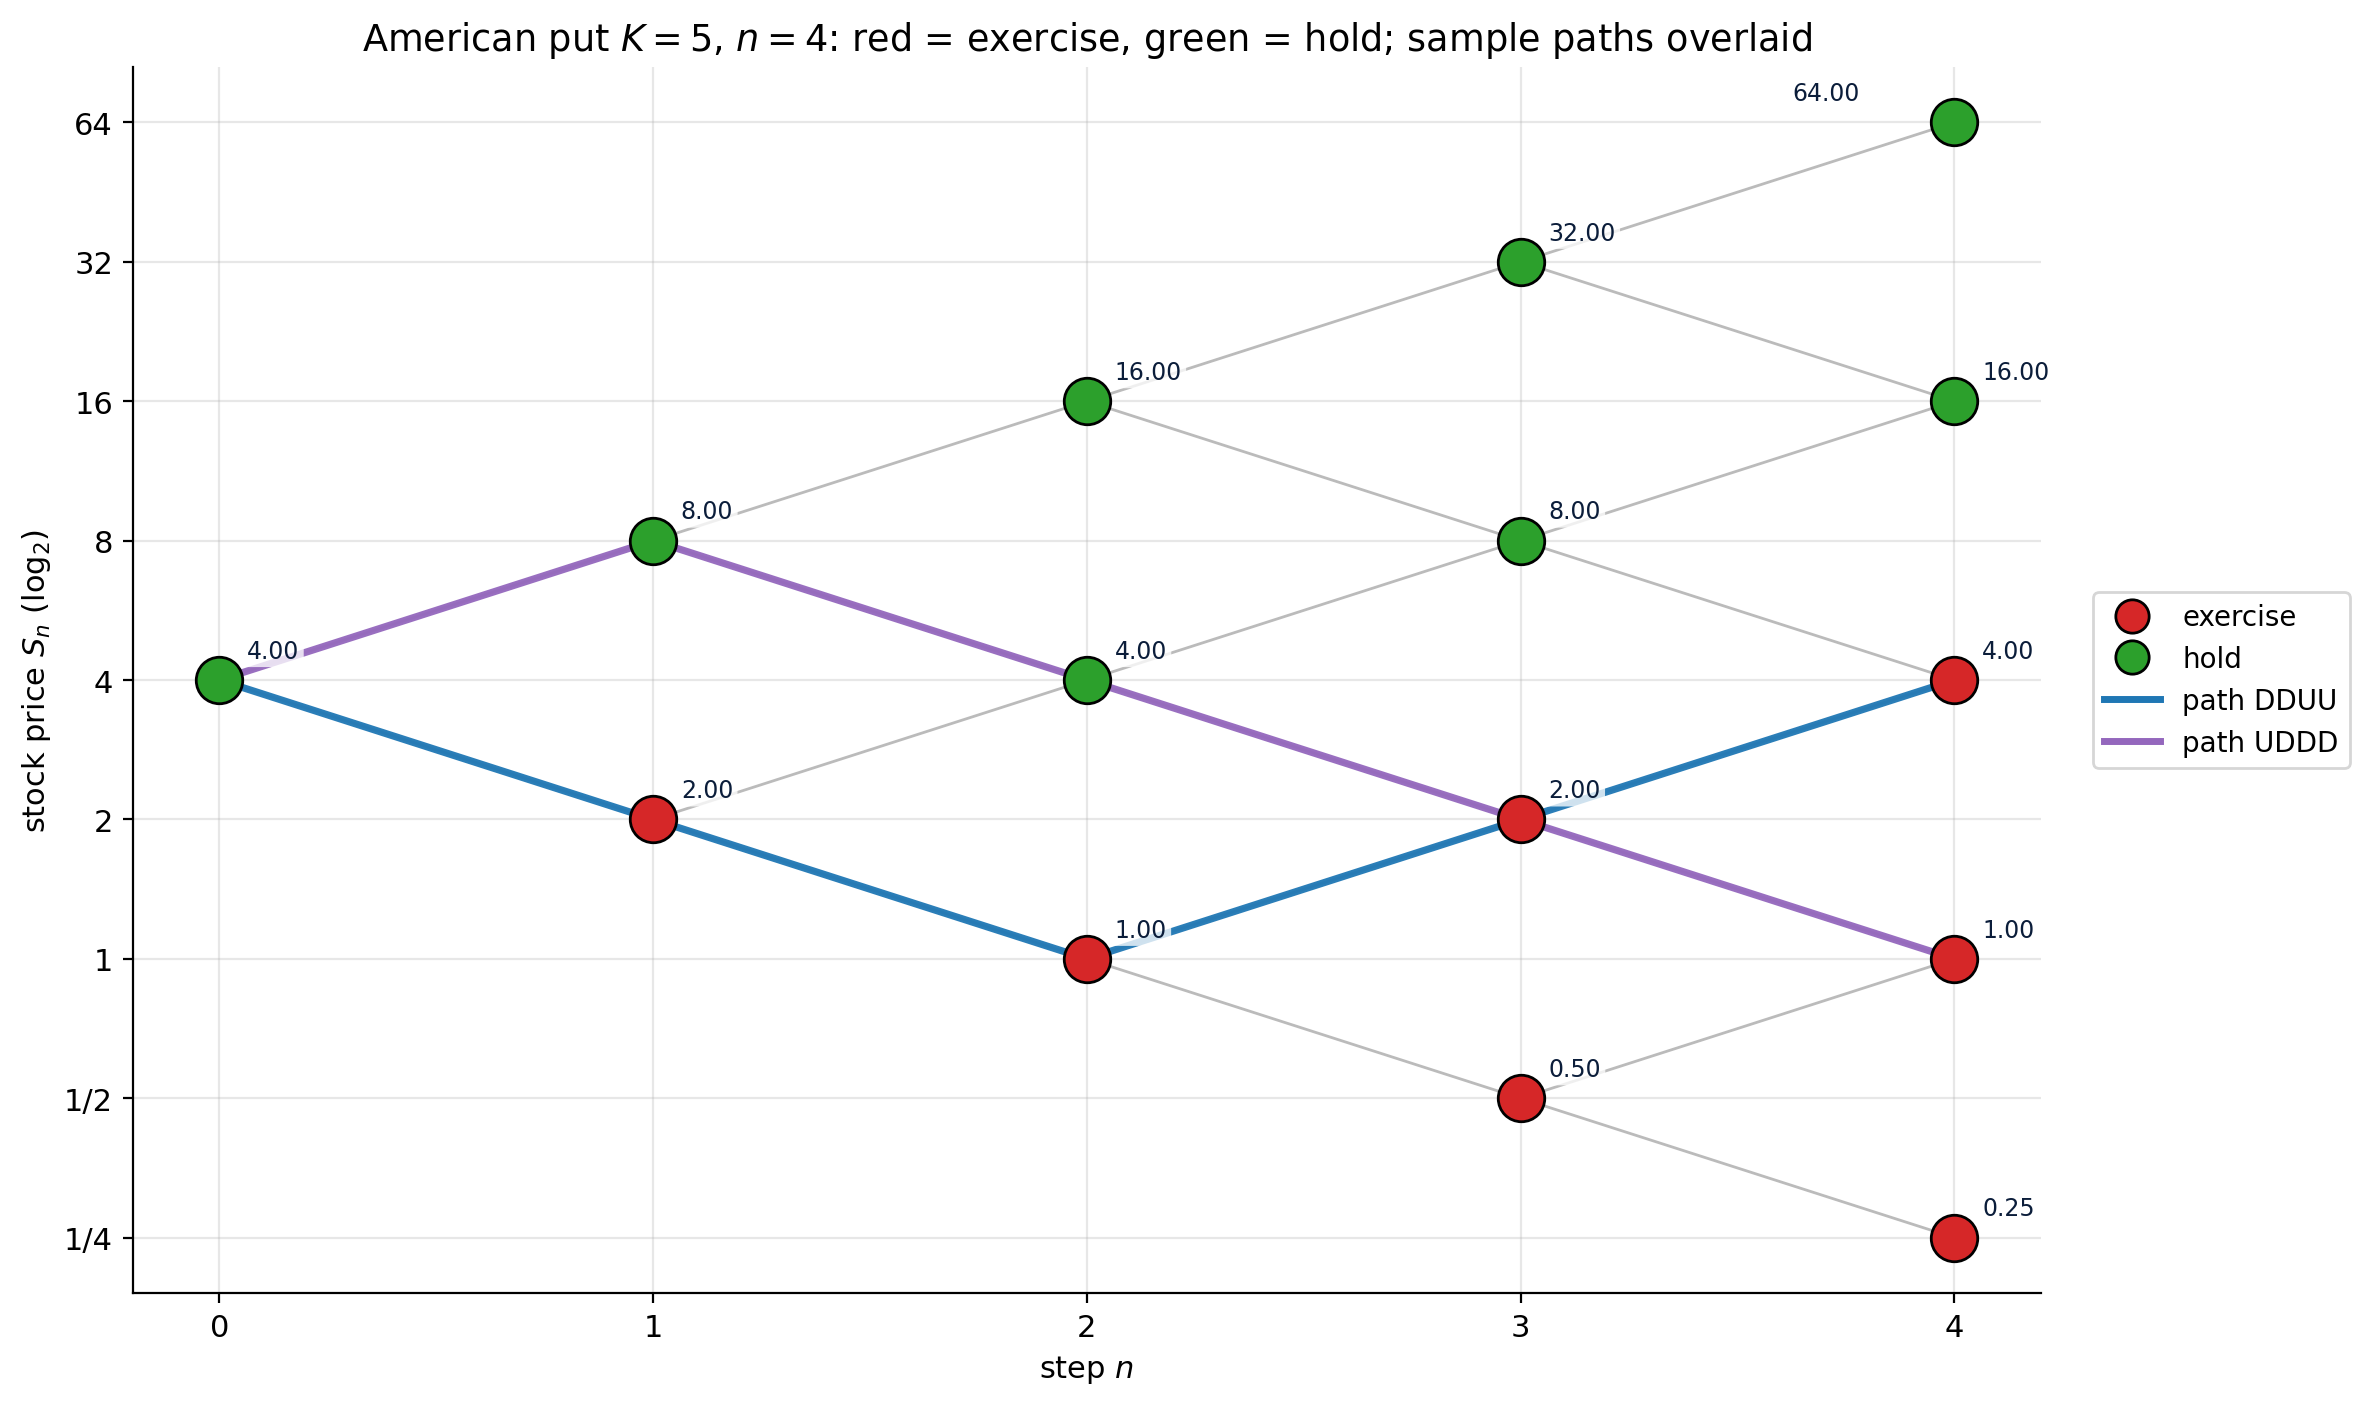
\includegraphics[keepaspectratio]{figures/ch05-am-frontier-paths.png}}
\caption{American put, \(K = 5\), \(n = 4\). Red nodes are
optimal-exercise nodes; green are hold-and-continue. Two sample paths
(blue DDUU, purple UDDD) overlaid; the purple path ends in the exercise
region, the blue stays out.}
\end{figure}

\subsection{5.8.2 Exercises}\label{exercises-26}

\begin{enumerate}
\def\labelenumi{\arabic{enumi}.}
\tightlist
\item
  In Example 5.8.1, identify by enumeration which of the 16 length-4
  paths first enter the exercise region. \textbf{Answer:} Paths that
  visit \(S = 1\) or \(S = 0.25\) before \(n = 4\): DDU? (goes to
  \(S = 1\) at \(n = 2\)), DDD-anything, etc.
\item
  Argue that the American call on a non-dividend-paying stock equals the
  European call. \textbf{Answer:} The intrinsic value \((S - K)^+\) is
  dominated by the continuation \((S(1+r) - K \cdot (1+r)^{?})^+\) at
  non-negative \(r\) --- so the exercise region is empty for the call.
  This is the standard no-early-exercise theorem (also covered in Ch 4).
\end{enumerate}

\begin{center}\rule{0.5\linewidth}{0.5pt}\end{center}

\section{§5.9 Asymptotics: from random walk to bell
curve}\label{asymptotics-from-random-walk-to-bell-curve}

\textbf{Punchline.} As \(n \to \infty\), the random walk's distribution
smooths into a normal bell curve (Central Limit Theorem). The reflection
principle's prediction for \(\mathbb P(M_n \ge m)\) converges to the
continuous-time identity
\(\mathbb P(\sup_{0 \le t \le T} W_t \ge m) = 2 \mathbb P(W_T \ge m) = 2 (1 - \Phi(m/\sqrt T))\).

\textbf{Intuition.} Zoom out on a high-\(n\) random walk and it looks
like a noisy continuous curve. Levels \(m\) and times \(n\) both
rescale; the natural scaling is ``\(m\) proportional to \(\sqrt n\)''
--- because that's the standard deviation of \(X_n\). Set
\(a = m/\sqrt n\); then the discrete formulas converge to continuous
ones in \(a\).

\subsection{5.9.1 The CLT for the random
walk}\label{the-clt-for-the-random-walk}

From Chapter 0 §0.10, \(X_n / \sqrt n\) converges in distribution to a
standard normal \(N(0, 1)\):

\[\mathbb P(X_n / \sqrt n \le a) \;\to\; \Phi(a) \qquad \text{as } n \to \infty.\]

So \(\mathbb P(X_n \ge a\sqrt n) \to 1 - \Phi(a)\).

\subsection{5.9.2 The asymptotic max law}\label{the-asymptotic-max-law}

From Corollary 1 of §5.3 in its sharp form:

\[\mathbb P(M_n \ge m) \;=\; 2\,\mathbb P(X_n \ge m) \;-\; \mathbb P(X_n = m).\]

Setting \(m = a\sqrt n\) and letting \(n \to \infty\): the atom
\(\mathbb P(X_n = a\sqrt n)\) decays like \(1/\sqrt n\) (by the local
CLT) and \emph{vanishes in the limit}, while
\(\mathbb P(X_n \ge a\sqrt n) \to 1 - \Phi(a)\). Therefore

\[\boxed{\;\mathbb P(M_n \ge a\sqrt n) \;\longrightarrow\; 2\,(1 - \Phi(a)) \qquad \text{as } n \to \infty.\;}\]

\textbf{The clean continuous-time identity.} For standard Brownian
motion \(W_t\) with \(W_0 = 0\) and any \(u > 0\):

\[\mathbb P\bigl(\sup_{0 \le t \le T} W_t \ge u\bigr) \;=\; 2\,\mathbb P(W_T \ge u) \;=\; 2(1 - \Phi(u/\sqrt T)).\]

\emph{No continuity correction is needed in the continuous limit} ---
the atom \(\mathbb P(W_T = u)\) is zero. In the discrete pre-limit walk
it is positive, and the \(-\mathbb P(X_n = m)\) term in Corollary 1 is
exactly the ``continuity correction'' that gets washed out by the CLT.
\emph{Reflection survives the limit; only the bookkeeping atom
disappears.}

\subsection{5.9.3 Examples}\label{examples-29}

\textbf{Example 5.9.1 (exact vs asymptotic at \(n = 100\), \(m = 10\)).}
Exact: \(\mathbb P(M_{100} \ge 10) = 0.3197\) (computer). Asymptotic:
\(2(1 - \Phi(1)) = 2 \cdot 0.1587 = 0.3173\). Relative error \(0.75\%\)
--- excellent.

\textbf{Example 5.9.2 (\(n = 100\), \(m = 20\)).} Exact: \(0.0460\).
Asymptotic: \(2(1 - \Phi(2)) = 2 \cdot 0.0228 = 0.0455\). Relative error
\(1\%\). The tail of the distribution agrees too, despite the rare-event
regime.

\textbf{Example 5.9.3 (\(n = 100\), \(m = 30\)).} Exact:
\(\approx 0.0027\). Asymptotic:
\(2(1 - \Phi(3)) = 2 \cdot 0.00135 = 0.0027\). Three-sigma agreement.

\begin{figure}
\centering
\pandocbounded{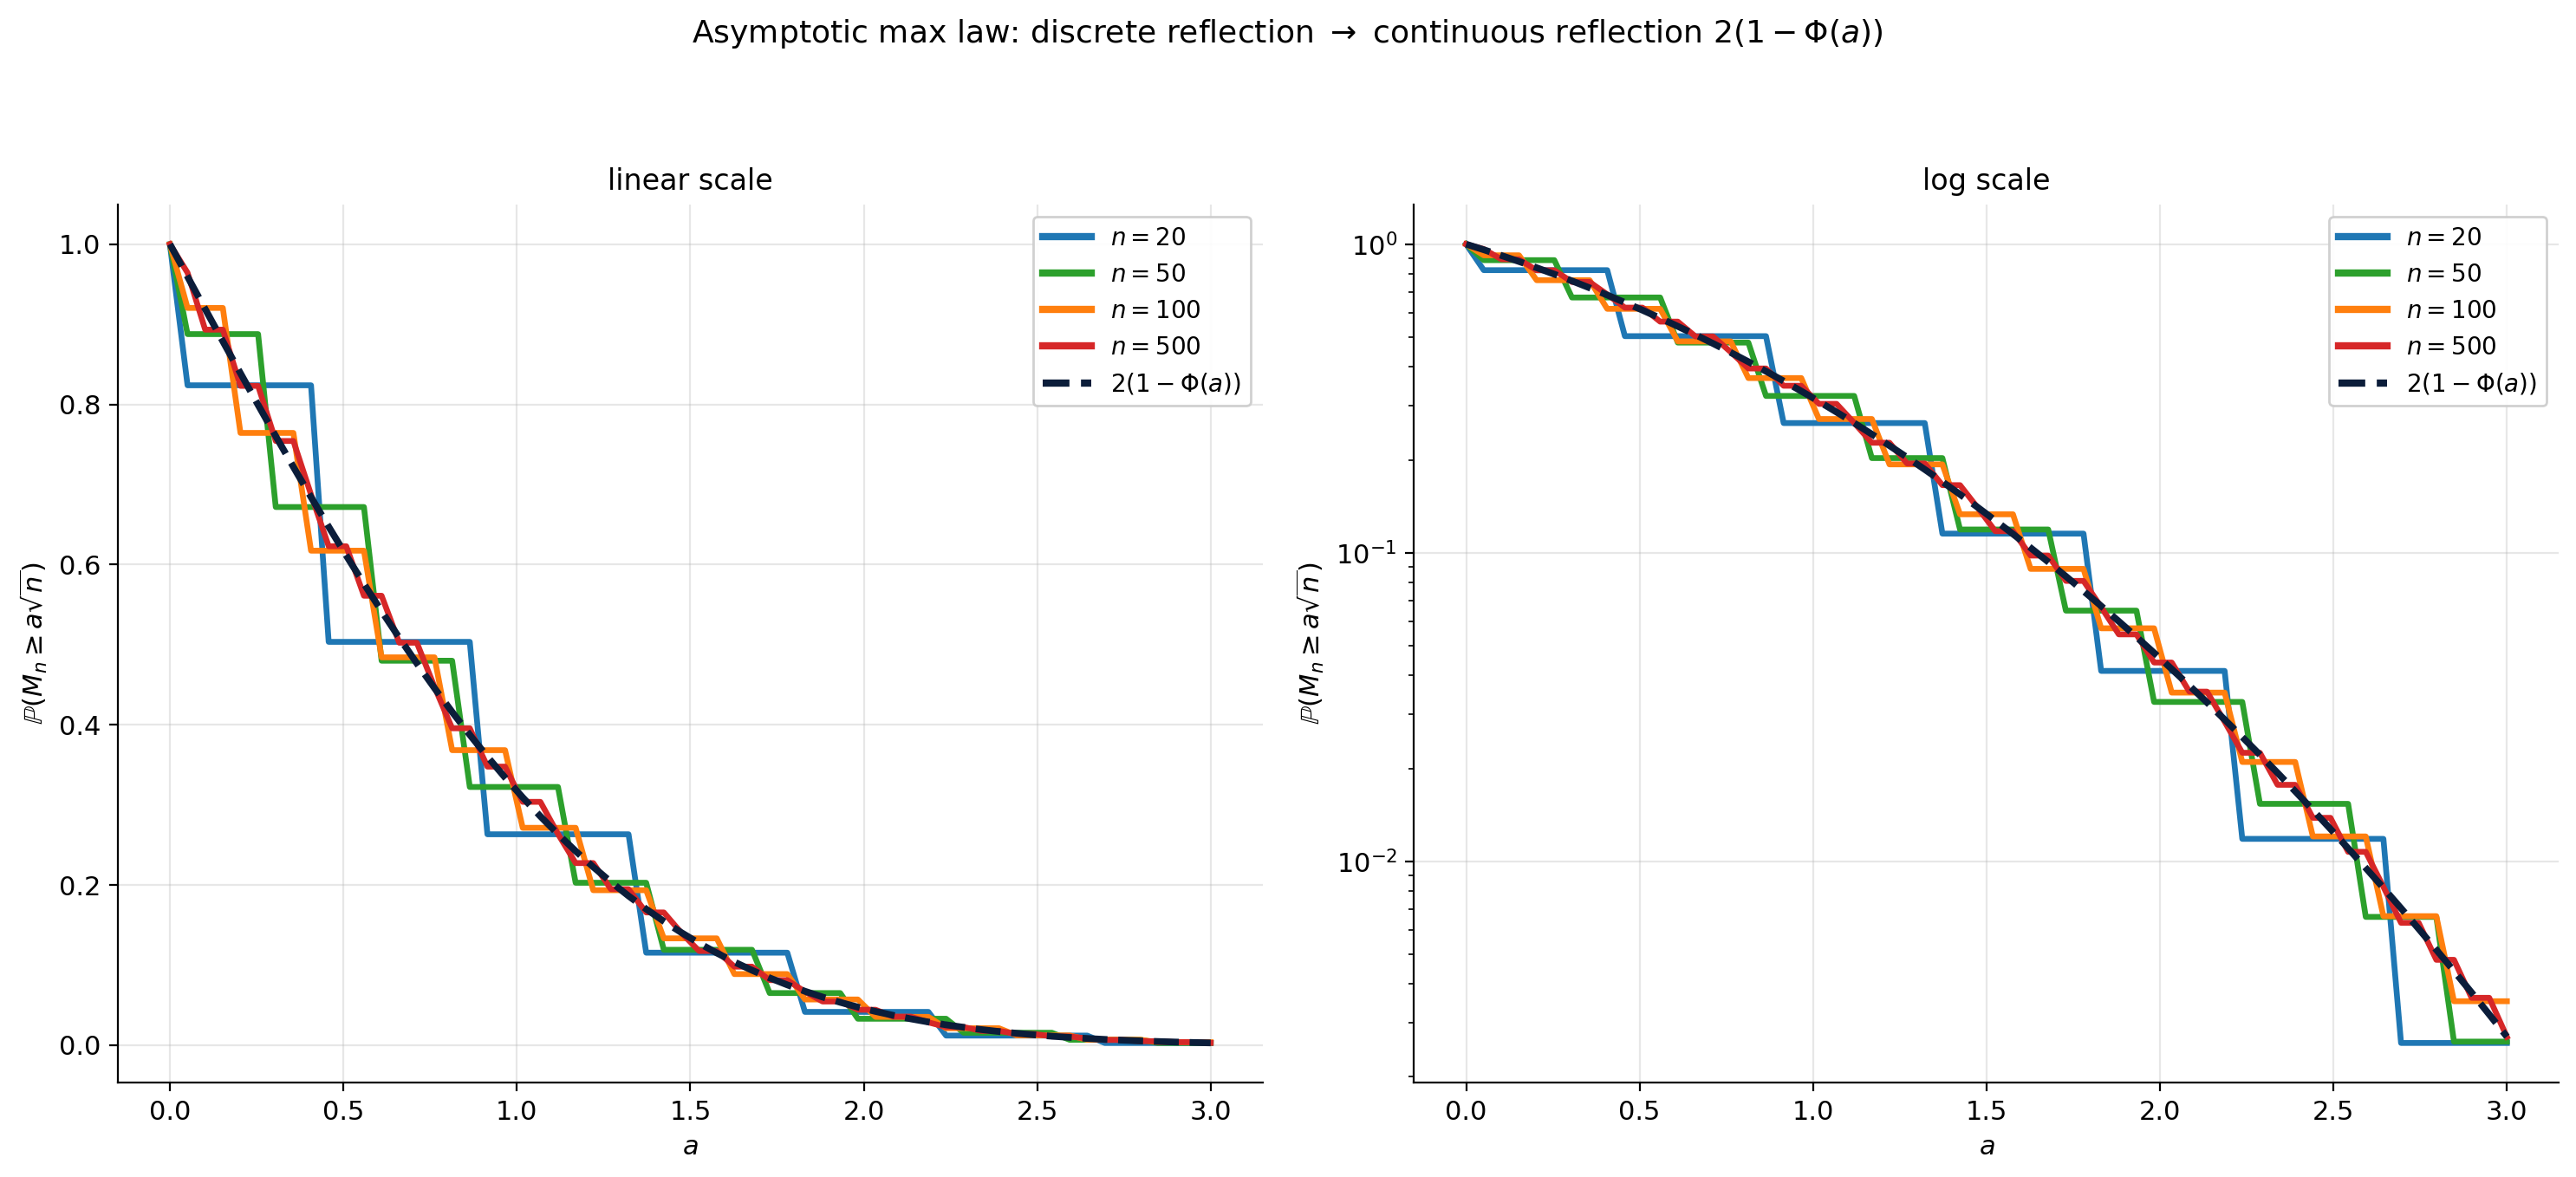
\includegraphics[keepaspectratio]{figures/ch05-Mn-asymptotic-2panel.png}}
\caption{Two panels showing \(\mathbb P(M_n \ge a\sqrt n)\) for
\(n = 20, 50, 100, 500\), with the limiting curve \(2(1 - \Phi(a))\)
overlaid (navy dashed). Linear scale (left) and log scale (right) ---
the log scale shows the convergence is uniform in the tails.}
\end{figure}

\begin{figure}
\centering
\pandocbounded{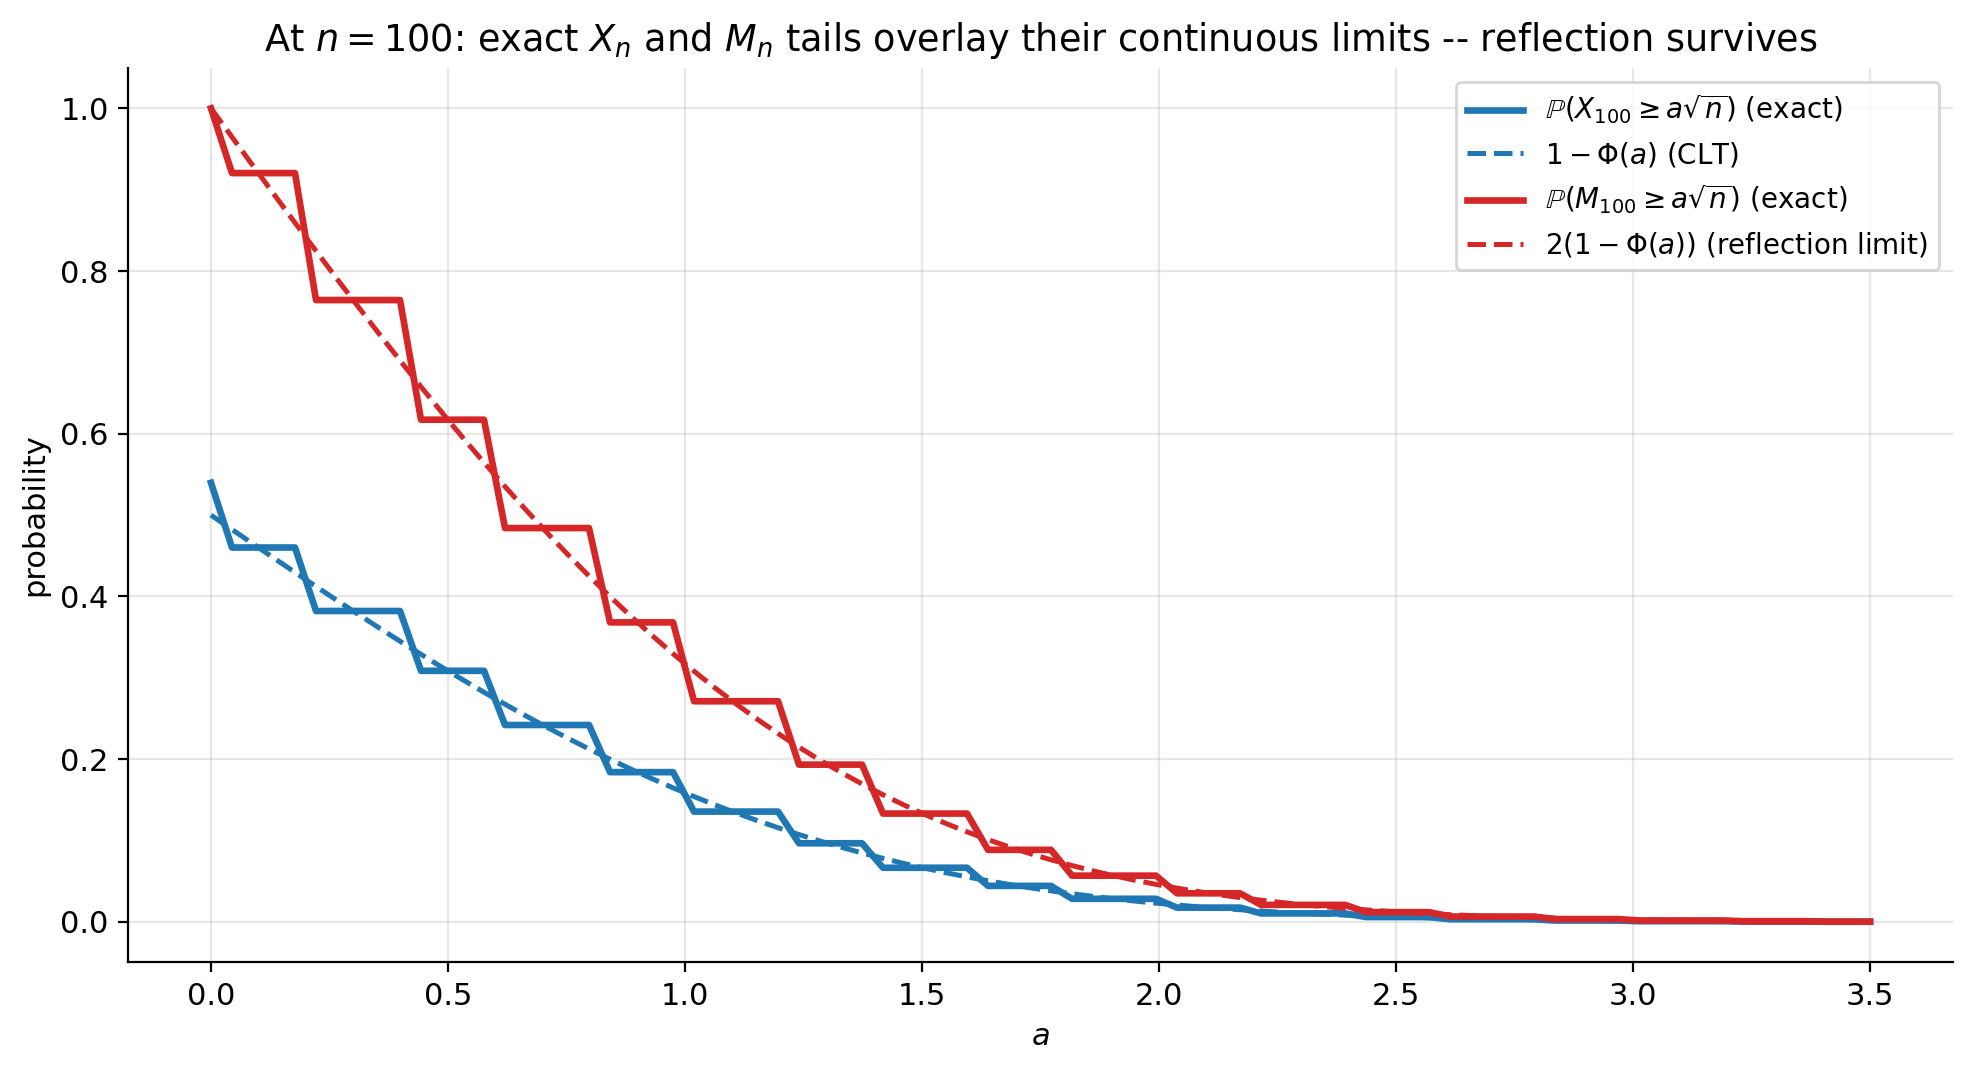
\includegraphics[keepaspectratio]{figures/ch05-clt-reflection-curves.png}}
\caption{At \(n = 100\) already, both the marginal of \(X_n\) (blue) and
the marginal of \(M_n\) (red) overlay their CLT/reflection limits. The
factor-of-2 gap between blue and red is the reflection signature.}
\end{figure}

\subsection{5.9.4 Tables}\label{tables-18}

\textbf{Table 5.13.} Exact \(\mathbb P(M_n \ge a\sqrt n)\) vs asymptotic
\(2(1 - \Phi(a))\).

{\def\LTcaptype{none} % do not increment counter
\begin{table}[H]
\centering
\begin{tabular}{|l|r|r|r|r|r|r|}
\toprule
\(n\) ~\(a\) & \(0.5\) & \(1.0\) & \(1.5\) & \(2.0\) & \(2.5\) & \(3.0\) \\
\midrule



\(20\) & \(0.6488\) & \(0.3851\) & \(0.1796\) & \(0.0709\) & \(0.0207\)
& \(0.0047\) \\
\(50\) & \(0.6314\) & \(0.3454\) & \(0.1471\) & \(0.0539\) & \(0.0167\)
& \(0.0040\) \\
\(100\) & \(0.6235\) & \(0.3197\) & \(0.1351\) & \(0.0460\) & \(0.0125\)
& \(0.0027\) \\
\(500\) & \(0.6195\) & \(0.3208\) & \(0.1369\) & \(0.0457\) & \(0.0125\)
& \(0.0027\) \\
\textbf{limit} \(2(1-\Phi(a))\) & \(\mathbf{0.6171}\) &
\(\mathbf{0.3173}\) & \(\mathbf{0.1336}\) & \(\mathbf{0.0455}\) &
\(\mathbf{0.0124}\) & \(\mathbf{0.0027}\) \\
\bottomrule
\end{tabular}
\end{table}
}

The convergence is monotone-ish (with small fluctuations from the parity
constraint) and at \(n = 500\) the agreement is good to four decimal
places across the full range of \(a\).

\begin{center}\rule{0.5\linewidth}{0.5pt}\end{center}

\section{§5.10 Reflection bridge to Black-Scholes
barriers}\label{reflection-bridge-to-black-scholes-barriers}

\textbf{Punchline.} The continuous-time Brownian motion \(W_t\) inherits
a reflection principle:

\[\mathbb P\bigl(\,\sup_{0 \le t \le T} W_t \ge m,\; W_T \le h\,\bigr) \;=\; \mathbb P\bigl(W_T \ge 2m - h\bigr), \qquad h \le m.\]

This is the same identity as the discrete one, with \(X_n\) replaced by
\(W_T\). The reason it survives is precisely the limit theorem from §5.9
--- the discrete reflection bijection has a continuous-time analogue,
namely ``reflect Brownian sample paths across the level \(m\) after the
first hit.''

\subsection{5.10.1 The Black-Scholes up-and-in
call}\label{the-black-scholes-up-and-in-call}

For Geometric Brownian motion \(S_t = S_0 \exp(\mu t + \sigma W_t)\)
with up-and-in call barrier \(L > S_0 > K\), the price formula is (we
state, do not derive):

\[\begin{aligned}
V^{\text{KI, up-call}} = \; & S_0 (L/S_0)^{2\lambda} N(y) \\
& - K e^{-rT} (L/S_0)^{2\lambda - 2} N(y - \sigma\sqrt T),
\end{aligned}\]

where \(\lambda = (r + \sigma^2/2)/\sigma^2\) and \(y\) is a particular
log-moneyness combination involving \(L, K, S_0, r, \sigma, T\). (The
exact form:
\(y = \ln(L^2 / (S_0 K)) / (\sigma\sqrt T) + \lambda \sigma\sqrt T\).)
The full derivation requires the continuous reflection principle plus
Girsanov change-of-measure --- material for Chapter 7 of the \emph{full
quant course}. What matters here:

\begin{itemize}
\tightlist
\item
  \textbf{The factor \((L/S_0)^{2\lambda}\)} is \emph{the
  continuous-time analogue of the discrete reflection coefficient
  \(\binom{n}{(n + 2m - h)/2}/\binom{n}{(n+h)/2}\).} In discrete
  reflection, ``doubling'' the barrier overshoots gave us \(2m - h\); in
  continuous, the analog is the power-law factor.
\item
  \textbf{Every barrier formula in Black-Scholes-Merton has
  reflection-principle DNA}: an up-and-in call, an up-and-out call, a
  down-and-out put, a one-touch digital --- all involve the factor
  \((L/S_0)^{2\lambda}\) or its variant, which \emph{is} the reflection
  identity in continuous-time clothing.
\end{itemize}

\subsection{5.10.2 Closing punchline}\label{closing-punchline}

\textbf{Reflection is a counting argument. It works in every dimension
and every time scale.}

We have used reflection to:

\begin{itemize}
\tightlist
\item
  Count discrete lattice paths (§5.3).
\item
  Derive first-passage time distributions (§5.4).
\item
  Compute joint \((M_n, X_n)\) pmfs (§5.5).
\item
  Price knock-in / knock-out barrier options on the binomial tree
  (§5.6).
\item
  Price lookback options (§5.7).
\item
  Anticipate the continuous Black-Scholes barrier formula (§5.10).
\end{itemize}

What unites all these applications is the same picture: \emph{every path
that does \(X\) corresponds, via reflection, to exactly one path that
does \(Y\)}. The combinatorics never gets more complex than counting
endpoints, even when the question is about whole paths. That is the
value proposition of the random-walk model.

\begin{center}\rule{0.5\linewidth}{0.5pt}\end{center}

\section{Chapter summary}\label{chapter-summary-2}

{\def\LTcaptype{none} % do not increment counter
\begin{table}[H]
\centering
\begin{tabular}{|l|l|}
\toprule
Concept & Where used \\
\midrule



Symmetric random walk \(X_n\) & everywhere \\
Running maximum \(M_n\) & barriers, lookbacks \\
Reflection identity & §5.3, §5.5, §5.6 \\
Max marginal & barrier counts \\
Joint pmf & §5.5 \\
First-passage time & §5.4 \\
In-out parity & §5.6 \\
Asymptotic max & §5.9, §5.10 \\
\bottomrule
\end{tabular}
\end{table}
}

\textbf{Definitions.} - \emph{Symmetric random walk}:
\(X_n = \xi_1 + \cdots + \xi_n\) with \(\xi_i = \pm 1\) fair. -
\emph{Running maximum}: \(M_n = \max_{0 \le k \le n} X_k\). -
\emph{Reflection identity}:
\(\mathbb P(M_n \ge m, X_n = h) = \mathbb P(X_n = 2m - h)\) for
\(h \le m\). - \emph{Max marginal}:
\(\mathbb P(M_n \ge m) = 2\,\mathbb P(X_n \ge m) - \mathbb P(X_n = m)\)
(equivalently \(\mathbb P(X_n \ge m) + \mathbb P(X_n \ge m+1)\) --- the
\(-\mathbb P(X_n = m)\) is the discrete ``continuity correction'' that
vanishes in the continuous limit). - \emph{Joint pmf}:
\(\mathbb P(M_n = m, X_n = h) = \mathbb P(X_n = 2m-h) - \mathbb P(X_n = 2m-h+2)\).
- \emph{First-passage time}:
\(\mathbb P(\tau_m = n) = (m/n)\mathbb P(X_n = m)\). - \emph{In-out
parity}: \(V^{\text{KI}} + V^{\text{KO}} = V^{\text{vanilla}}\). -
\emph{Asymptotic max}:
\(\mathbb P(M_n \ge a\sqrt n) \to 2(1 - \Phi(a))\).

\begin{center}\rule{0.5\linewidth}{0.5pt}\end{center}

\section{Bridge to Chapter 6}\label{bridge-to-chapter-6}

We have built equity-payoff machinery: vanilla, barrier, lookback,
American --- all priced on a binomial tree, with the reflection
principle as the indispensable counting tool. Every payoff so far has
been a function of equity \emph{prices} and (sometimes) the equity
\emph{path}.

\textbf{But the discount factor \((1+r)^{-n}\) has been a constant.}
That implicitly assumes a deterministic interest rate. In reality, rates
fluctuate --- and that fluctuation drives a whole asset class:
\emph{bonds} and \emph{interest-rate derivatives}. Bond prices do not
depend on equity prices; they depend on \emph{the path of rates}.

Chapter 6 puts rates onto a binomial tree. We will:

\begin{itemize}
\tightlist
\item
  Define the short-rate process \(r_n\) as a tree-valued random
  variable.
\item
  Build the simplest interest-rate tree (the Ho-Lee model, in discrete
  form).
\item
  Price a zero-coupon bond as the \emph{expected discounted unit
  cashflow under the risk-neutral rate-tree}.
\item
  Discover that bond pricing under a stochastic short-rate is \emph{the
  same algorithm} as equity pricing under a stochastic stock-tree ---
  replace stock by rate, replace stock payoff by bond payoff.
\item
  See how the random-walk and reflection ideas from this chapter carry
  over: rate-path-dependent payoffs (e.g., caps and floors) reduce to
  counting on the rate tree.
\end{itemize}

The bridge is conceptual: \emph{every Chapter-2-style risk-neutral
pricing argument applies to any process you can put on a binomial tree}.
We have so far put one asset (stock) on the tree. Chapter 6 puts another
(rate) on its own tree. Chapter 7 will combine both into the
Black-Scholes limit.

\emph{Onward.}

\newpage

\chapter{Chapter 6 --- Interest-Rate-Dependent Securities on a Binomial
Tree}\label{chapter-6-interest-rate-dependent-securities-on-a-binomial-tree}

\section{How this chapter works}\label{how-this-chapter-works}

Up to this point the underlying random object in every tree was a
\emph{stock}: a price that went up by a factor \(u\) or down by a factor
\(d\). Everything that mattered was driven by that one price, and the
discount factor \((1+r)^{-1}\) was a constant we slipped in without much
comment.

This chapter swaps the underlying. The random object is now a
\textbf{short rate} \(r_n\) --- the one-period interest rate at node
\(n\). It still lives on a binomial tree, but now every pricing identity
in Chapters 1-5 needs the discount factor to move \emph{with} the tree.
The big payoff: we get zero-coupon bonds, yield curves, forward rates,
caplets, caps, floors, bond options, swaps, and a first taste of
calibration --- all without a single calculus operation.

I'll use two running toys throughout the chapter, the same two we'll
re-use in Chapter 7's calibration drills:

\begin{itemize}
\tightlist
\item
  \textbf{Toy-A} (numbered, big moves): \(r_0 = 0.25\), \(u = 2\),
  \(d = 0.5\), \(\tilde p = 1/2\).
\item
  \textbf{Realistic-B} (closer to market rates): \(r_0 = 5\%\),
  \(u = 1.25\), \(d = 0.8\), \(\tilde p = 1/2\).
\end{itemize}

Toy-A makes the arithmetic ugly enough to \emph{see} that something
nontrivial is happening. Realistic-B makes the prices look like prices a
desk would quote. Every section computes both.

The shape of every section is the same shape as Chapters 0-5:
\textbf{punchline}, \textbf{intuition} callout, definitions, numbered
numbered examples, figures, tables, exercises with answers.

\begin{center}\rule{0.5\linewidth}{0.5pt}\end{center}

\section{§6.1 The short-rate binomial
tree}\label{the-short-rate-binomial-tree}

\textbf{Punchline.} Build a binomial tree whose nodes are \emph{interest
rates}, not stock prices. The one-period rate at node \(n\), call it
\(r_n\), multiplies up by \(u_n\) on heads and down by \(d_n\) on tails.
The money-market account \(M_n\) rolls forward by \((1 + r_n)\), but the
crucial new wrinkle is that the discount factor is
\emph{path-dependent}: rolling \$1 forward from \(0\) to \(T\) no longer
gives the same number on every path.

\textbf{Intuition.} In Chapter 2 the stock multiplied by \(u\) or \(d\)
at each step. Replace the stock with the short rate and the same
machinery describes how \emph{rates} evolve. The catch: the short rate
at \(n\) tells you what \$1 grows to between \(n\) and \(n+1\). So the
multiplier between \(0\) and \(T\) is the \emph{product} of
\((1 + r_k)\) along whichever path you walked, and different paths land
at the same place by different multipliers. That is the entire new idea
of this chapter.

\subsection{6.1.1 Definitions}\label{definitions-17}

Fix a probability space generated by \(T\) coin tosses, exactly as in
Chapter 1. Let \(\omega = \omega_1 \omega_2 \cdots \omega_T\) be a path
with \(\omega_k \in \{H, T\}\).

\textbf{Short rate at \(n\).} The random variable \(r_n(\omega)\)
depends only on \(\omega_1, \ldots, \omega_n\) --- that is, \(r_n\) is
\textbf{adapted} to the natural filtration. In words: you know \(r_n\)
once you have seen the first \(n\) coin tosses, and not before.

\textbf{Recursion.} Given \(r_n\), the next step is

\[r_{n+1} \;=\; \begin{cases} u_n \, r_n & \text{on heads,} \\ d_n \, r_n & \text{on tails,} \end{cases}\]

with risk-neutral probabilities \(\tilde p\) and
\(\tilde q = 1 - \tilde p\). We'll allow \(u_n, d_n\) to depend on \(n\)
for §6.12; everywhere else they are constants \(u, d\).

\textbf{Money-market account.} Start with \(M_0 = 1\). Then

\[M_{n+1} \;=\; (1 + r_n)\, M_n, \qquad M_n \;=\; \prod_{k=0}^{n-1}(1 + r_k).\]

Notice \(M_n\) is \textbf{predictable}: \(M_n\) depends only on
\(r_0, \ldots, r_{n-1}\), so it is known at time \(n-1\). That asymmetry
--- \(r_n\) is adapted at \(n\), but \(M_n\) is known one step earlier
--- is the cleanest one-line definition of ``the short rate is the rate
\emph{over} the period that \emph{starts} at \(n\).''

\textbf{Path discount factor.} Define

\[D_n(\omega) \;=\; \frac{1}{M_n(\omega)} \;=\; \prod_{k=0}^{n-1} \frac{1}{1 + r_k(\omega)}.\]

This is the random discount factor for time \(n\): paying \$1 at time
\(n\) is worth \(D_n\) at time \(0\) \emph{conditional on having walked
path \(\omega\)}. The big difference from Chapters 1-5: \(D_n\) now
varies path-by-path.

\subsection{Intuition callout --- adapted vs
predictable}\label{intuition-callout-adapted-vs-predictable}

\begin{quote}
A quantity is \textbf{adapted} at \(n\) if you can compute it knowing
the first \(n\) flips. A quantity is \textbf{predictable} at \(n\) if
you can compute it knowing the first \(n-1\) flips. The short rate
\(r_n\) is adapted; the money-market account \(M_n\) is predictable.
Think of the short rate as a rate you \emph{learn} at the start of
period \(n\), and \(M_n\) as the value of \$1 you'd have \emph{already
accumulated} by then --- which only depends on rates you learned in
earlier periods.
\end{quote}

\subsection{6.1.2 Examples on Toy-A}\label{examples-on-toy-a}

Toy-A: \(r_0 = 0.25\), \(u = 2\), \(d = 0.5\), \(\tilde p = 1/2\),
recombining.

\textbf{Example 6.1.1 (one-step rate tree).} From \(r_0 = 0.25\):

\begin{itemize}
\tightlist
\item
  \(r_1(H) = u \, r_0 = 2 \cdot 0.25 = 0.50\).
\item
  \(r_1(T) = d \, r_0 = 0.5 \cdot 0.25 = 0.125\).
\end{itemize}

\textbf{Example 6.1.2 (two-step rate tree).} From the two \(n=1\) nodes:

\begin{itemize}
\tightlist
\item
  \(r_2(HH) = 2 \cdot 0.50 = 1.00\).
\item
  \(r_2(HT) = 0.5 \cdot 0.50 = 0.25\).
\item
  \(r_2(TH) = 2 \cdot 0.125 = 0.25\).
\item
  \(r_2(TT) = 0.5 \cdot 0.125 = 0.0625\).
\end{itemize}

The tree recombines: \(r_2(HT) = r_2(TH) = 0.25\). This is the same
recombining property we exploited in Chapter 2.

\textbf{Example 6.1.3 (three-step rate tree, all 8 paths).} Continuing
one more step:

{\def\LTcaptype{none} % do not increment counter
\begin{table}[H]
\centering
\begin{tabular}{|l|r|}
\toprule
Path & \(r_3\) \\
\midrule



HHH & \(2.0000\) \\
HHT & \(0.5000\) \\
HTH & \(0.5000\) \\
HTT & \(0.1250\) \\
THH & \(0.5000\) \\
THT & \(0.1250\) \\
TTH & \(0.1250\) \\
TTT & \(0.03125\) \\
\bottomrule
\end{tabular}
\end{table}
}

Four distinct \(r_3\) values: \(\{2, 0.5, 0.125, 0.03125\}\), with
multiplicities \(\binom{3}{k}\) for \(k = 3, 2, 1, 0\) heads.

\textbf{Example 6.1.4 (money-market along path HTH).} Toy-A,
\(r_0 = 0.25, r_1(H) = 0.50, r_2(HT) = 0.25, r_3(HTH) = 0.50\). The path
HTH stops at \(n = 3\), and \(M_3\) uses \(r_0, r_1, r_2\) --- not
\(r_3\).

\[M_1 = 1 + 0.25 = 1.25.\]
\[M_2 = 1.25 \cdot (1 + 0.50) = 1.25 \cdot 1.50 = 1.875.\]
\[M_3 = 1.875 \cdot (1 + 0.25) = 1.875 \cdot 1.25 = 2.34375.\]

So along HTH, \$1 invested at the money-market account grows to
\(\$2.34375\) in three periods.

\textbf{Example 6.1.5 (money-market along all 8 paths).} Filling in for
the full 8-path tree:

{\def\LTcaptype{none} % do not increment counter
\begin{table}[H]
\centering
\begin{tabular}{|l|r|r|r|r|}
\toprule
Path & \(r_0\) & \(r_1\) & \(r_2\) & \(M_3\) \\
\midrule



HHH & \(0.25\) & \(0.50\) & \(1.00\) & \(3.7500\) \\
HHT & \(0.25\) & \(0.50\) & \(1.00\) & \(3.7500\) \\
HTH & \(0.25\) & \(0.50\) & \(0.25\) & \(2.3438\) \\
HTT & \(0.25\) & \(0.50\) & \(0.25\) & \(2.3438\) \\
THH & \(0.25\) & \(0.125\) & \(0.25\) & \(1.7578\) \\
THT & \(0.25\) & \(0.125\) & \(0.25\) & \(1.7578\) \\
TTH & \(0.25\) & \(0.125\) & \(0.0625\) & \(1.4941\) \\
TTT & \(0.25\) & \(0.125\) & \(0.0625\) & \(1.4941\) \\
\bottomrule
\end{tabular}
\end{table}
}

\emph{Definition:} \(M_3 = (1+r_0)(1+r_1)(1+r_2)\). Sample products: HHH
gives \(1.25 \cdot 1.50 \cdot 2.00 = 3.7500\); HTH gives
\(1.25 \cdot 1.50 \cdot 1.25 = 2.3438\); THH gives
\(1.25 \cdot 1.125 \cdot 1.25 = 1.7578\); TTH gives
\(1.25 \cdot 1.125 \cdot 1.0625 = 1.4941\).

Two paths share each \(M_3\) value, because \(M_3\) depends only on the
first \emph{two} flips. (Predictability!)

\textbf{Example 6.1.6 (a non-recombining tree).} Take Toy-A but make the
rate factors path-dependent on purpose: let \(u_n = 2\) at every
up-node, but \(d_n = 0.25\) after one head and \(0.5\) after one tail.
Then \(r_2(HT) = 0.25 \cdot 0.50 = 0.125\) and
\(r_2(TH) = 2 \cdot 0.125 = 0.25\). They no longer agree. The tree is
\textbf{non-recombining}; the number of distinct \(n\)-step nodes grows
as \(2^n\) instead of \(n+1\). This chapter sticks with recombining
trees (constant \(u, d\) per step) except where flagged.

\textbf{Example 6.1.7 (negative rates are mathematically allowed).}
Nothing in the construction requires \(r_n > 0\). If the calibration
target (§6.12) drives \(\theta_n\) into negative territory we can still
build the tree and price bonds; only the money-market interpretation
gets weird. We will see this in §6.12.

\subsection{6.1.3 Examples on
Realistic-B}\label{examples-on-realistic-b}

Realistic-B: \(r_0 = 5\%\), \(u = 1.25\), \(d = 0.80\),
\(\tilde p = 1/2\). Note \(u \cdot d = 1\), so the tree is
\emph{log-symmetric} --- preview of Chapter 7's
\(u = e^{\sigma\sqrt{\Delta t}}, d = 1/u\).

\textbf{Example 6.1.8 (Realistic-B to \(n=3\)).} Building forward:

{\def\LTcaptype{none} % do not increment counter
\begin{table}[H]
\centering
\begin{tabular}{|l|r|r|r|r|}
\toprule
node & \(n = 0\) & \(n = 1\) & \(n = 2\) & \(n = 3\) \\
\midrule



top (\(H^n\)) & \(0.0500\) & \(0.0625\) & \(0.0781\) & \(0.0977\) \\
\(\binom{n}{1}\) & & \(0.0400\) & \(0.0500\) & \(0.0625\) \\
\(\binom{n}{2}\) & & & \(0.0320\) & \(0.0400\) \\
bottom (\(T^n\)) & & & & \(0.0256\) \\
\bottomrule
\end{tabular}
\end{table}
}

\emph{Tree is recombining: at level \(n\) the rate depends only on the
count of heads \(k\). Row \(k = 0\) is the all-\(H\) path (top); row
\(k = n\) is all-\(T\) (bottom). E.g.~at \(n=3\):
\(r_3(HHT) = r_3(HTH) = r_3(THH) = 0.0625\).}

A recombining tree. Realistic-B's \(n=2\) ladder is
\(\{0.0781, 0.0500, 0.0320\}\), log-symmetric around \(0.05\).

\textbf{Example 6.1.9 (Realistic-B \(M_3\) along all 8 paths).} Using
\(M_3 = (1 + r_0)(1 + r_1)(1 + r_2)\):

{\def\LTcaptype{none} % do not increment counter
\begin{table}[H]
\centering
\begin{tabular}{|l|r|r|r|r|}
\toprule
Path & \(r_0\) & \(r_1\) & \(r_2\) & \(M_3\) \\
\midrule



HH* & \(0.0500\) & \(0.0625\) & \(0.0781\) & \(1.20292\) \\
HT* & \(0.0500\) & \(0.0625\) & \(0.0500\) & \(1.17141\) \\
TH* & \(0.0500\) & \(0.0400\) & \(0.0500\) & \(1.14660\) \\
TT* & \(0.0500\) & \(0.0400\) & \(0.0320\) & \(1.12694\) \\
\bottomrule
\end{tabular}
\end{table}
}

\emph{Definition:} \(M_3 = (1+r_0)(1+r_1)(1+r_2)\). E.g.~HH\(*\):
\(1.05 \cdot 1.0625 \cdot 1.0781 = 1.20292\). TT\(*\):
\(1.05 \cdot 1.0400 \cdot 1.0320 = 1.12694\).

(The asterisk indicates the third flip is irrelevant for \(M_3\).)
Realistic-B's spread of \(M_3\) values is tighter than Toy-A's because
the rates are smaller. Already that's a useful intuition: realistic
interest-rate trees discount almost path-independently, so a
constant-rate model is an OK first approximation.

\begin{figure}
\centering
\pandocbounded{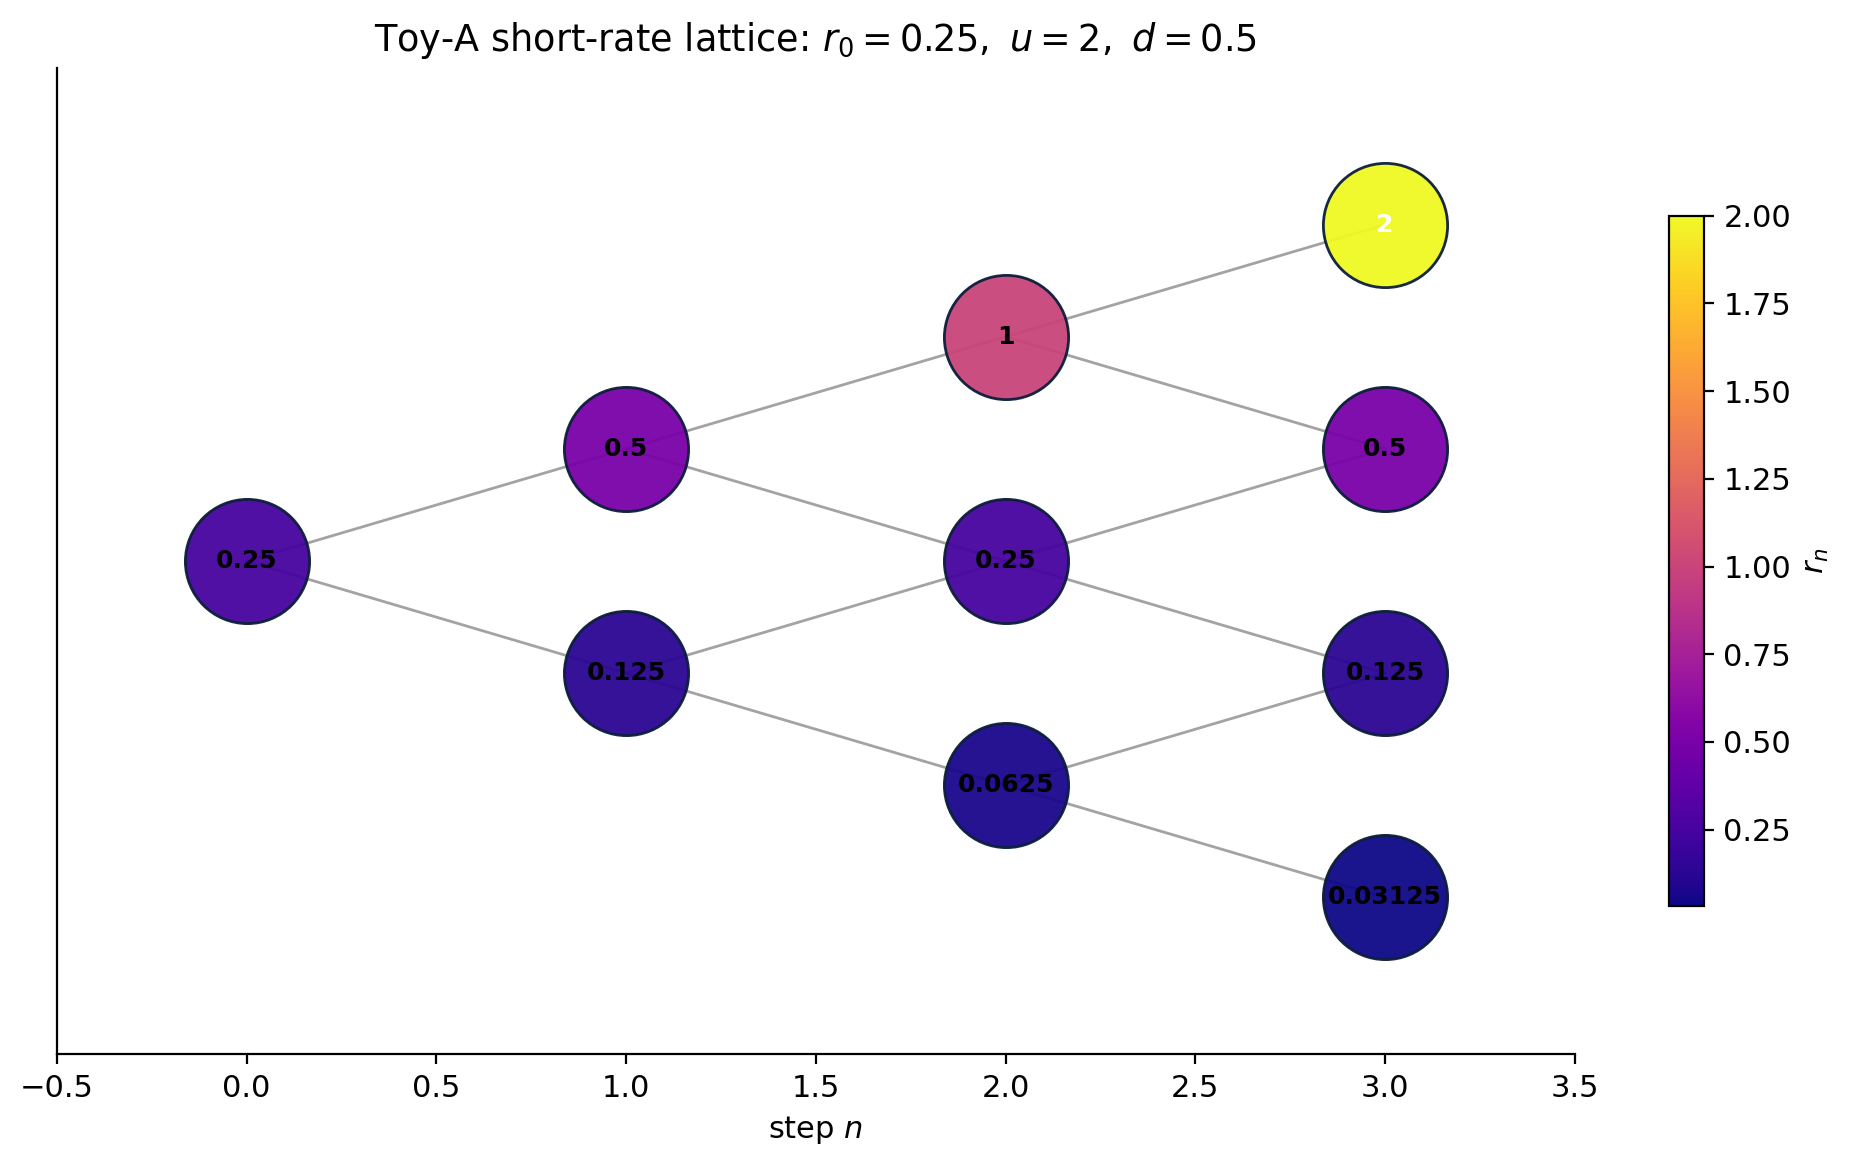
\includegraphics[keepaspectratio]{figures/ch06-rate-lattice-A.png}}
\caption{Figure 6.1 --- The Toy-A short-rate lattice through \(n=3\).
Each node is coloured by rate (cool = low, warm = high). The single
very-high node \(r_3(HHH) = 2.0\) is the lone red square in the
top-right.}
\end{figure}

\begin{figure}
\centering
\pandocbounded{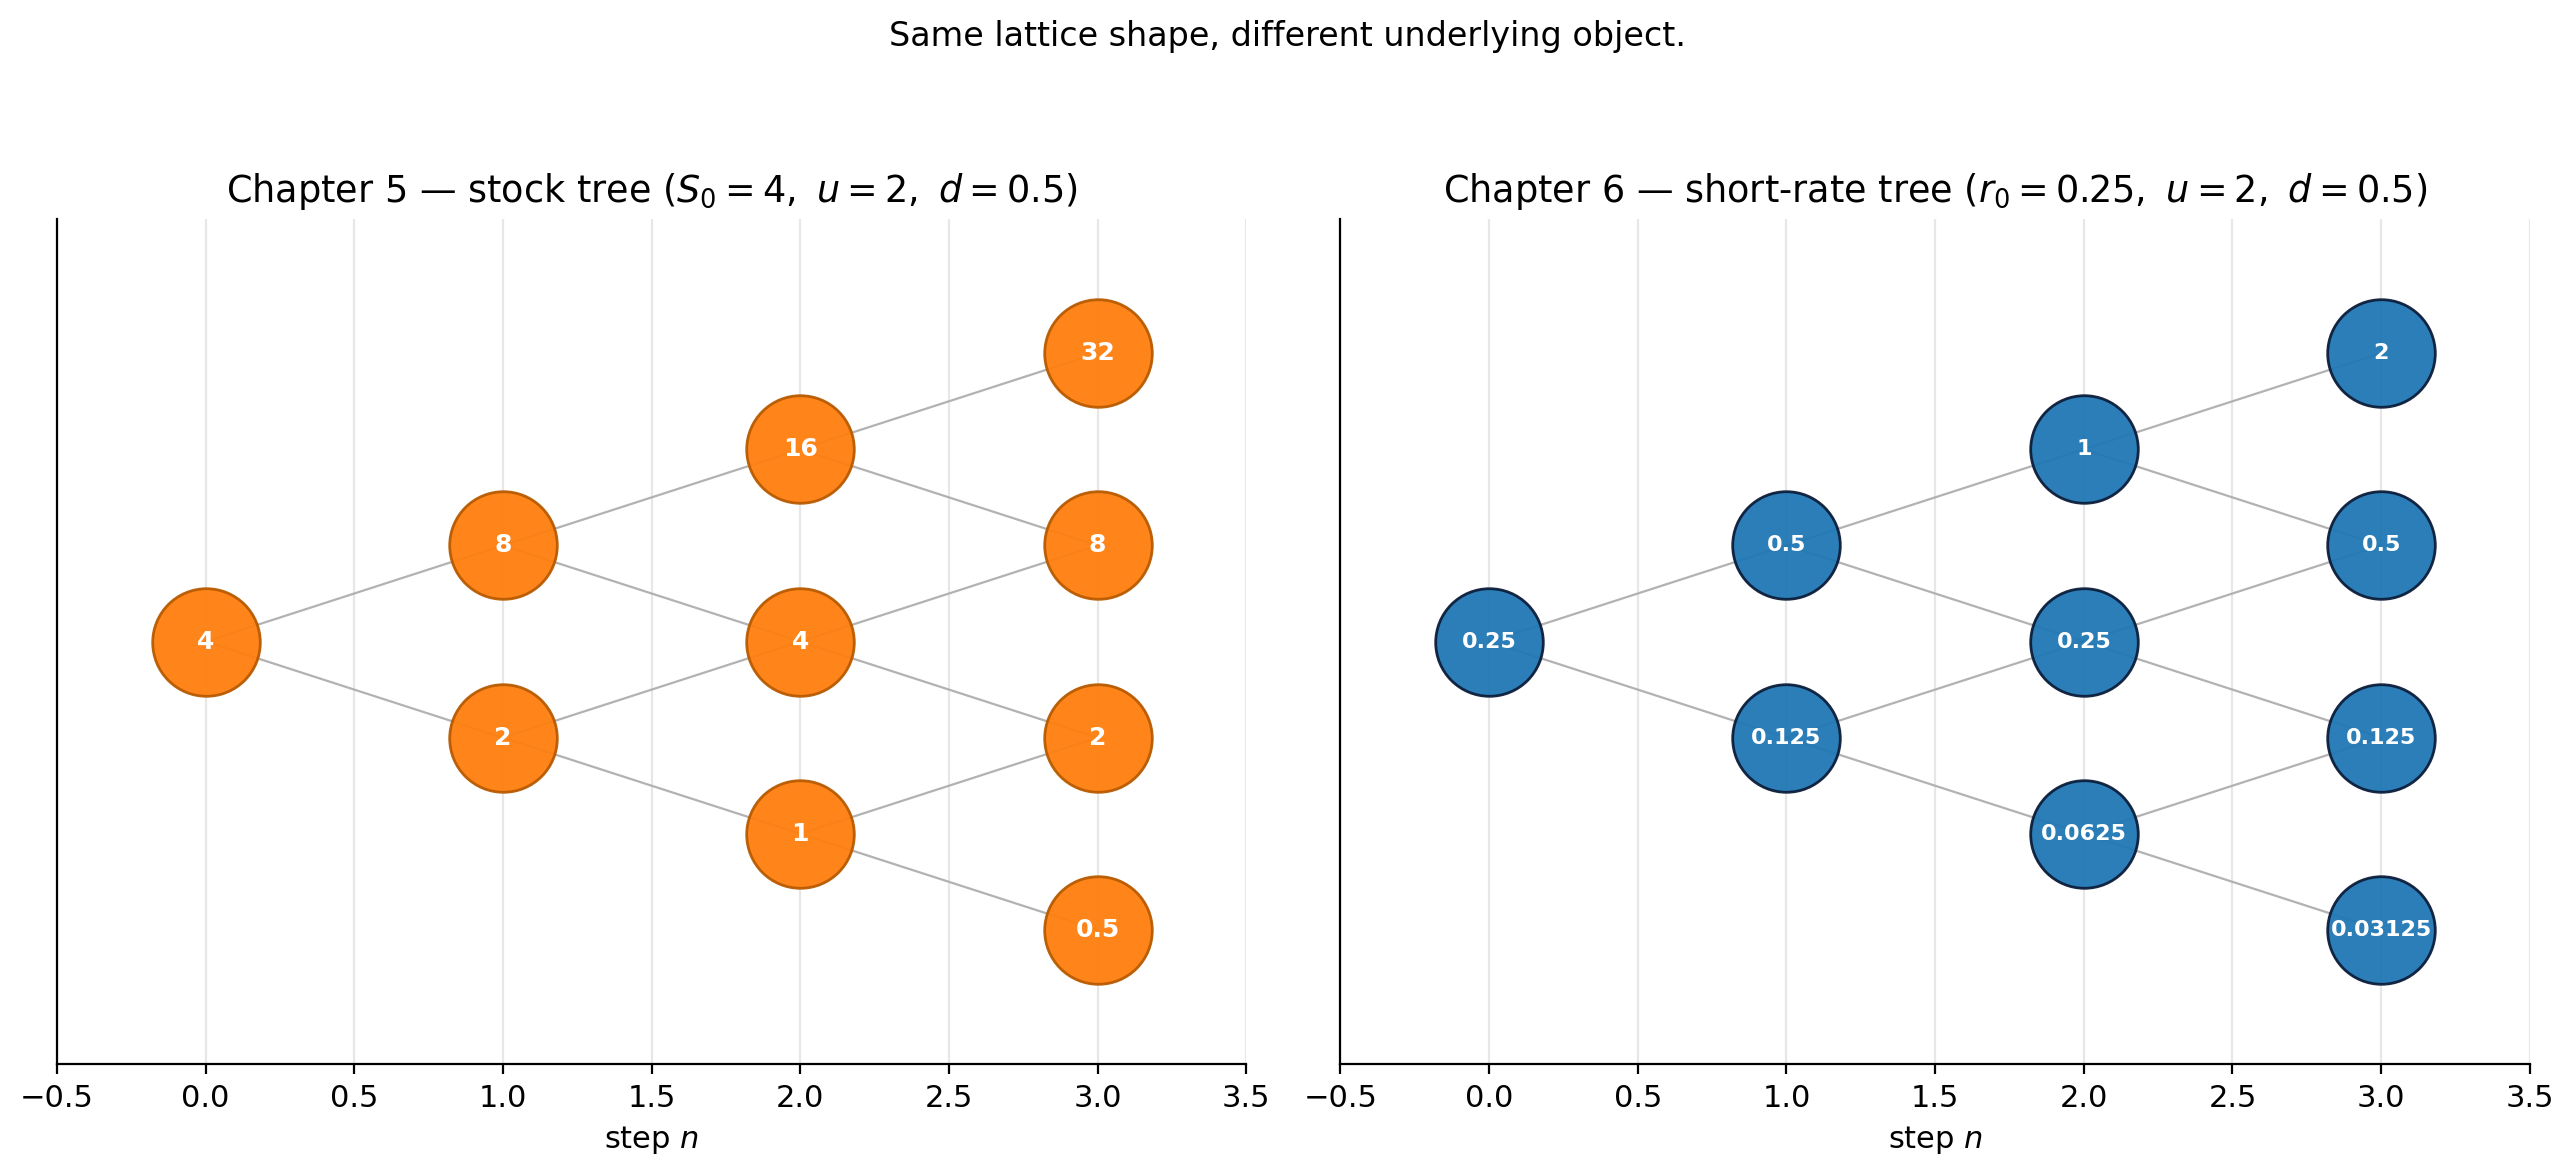
\includegraphics[keepaspectratio]{figures/ch06-stock-vs-rate-tree.png}}
\caption{Figure 6.2 --- Chapter 5 (stock) vs Chapter 6 (short rate)
trees side-by-side. Identical \emph{shape}, completely different
interpretation. The stock tree's nodes feed \emph{payoff} calculations;
the rate tree's nodes feed \emph{discounting} calculations. That's the
whole transition this chapter forces.}
\end{figure}

\begin{figure}
\centering
\pandocbounded{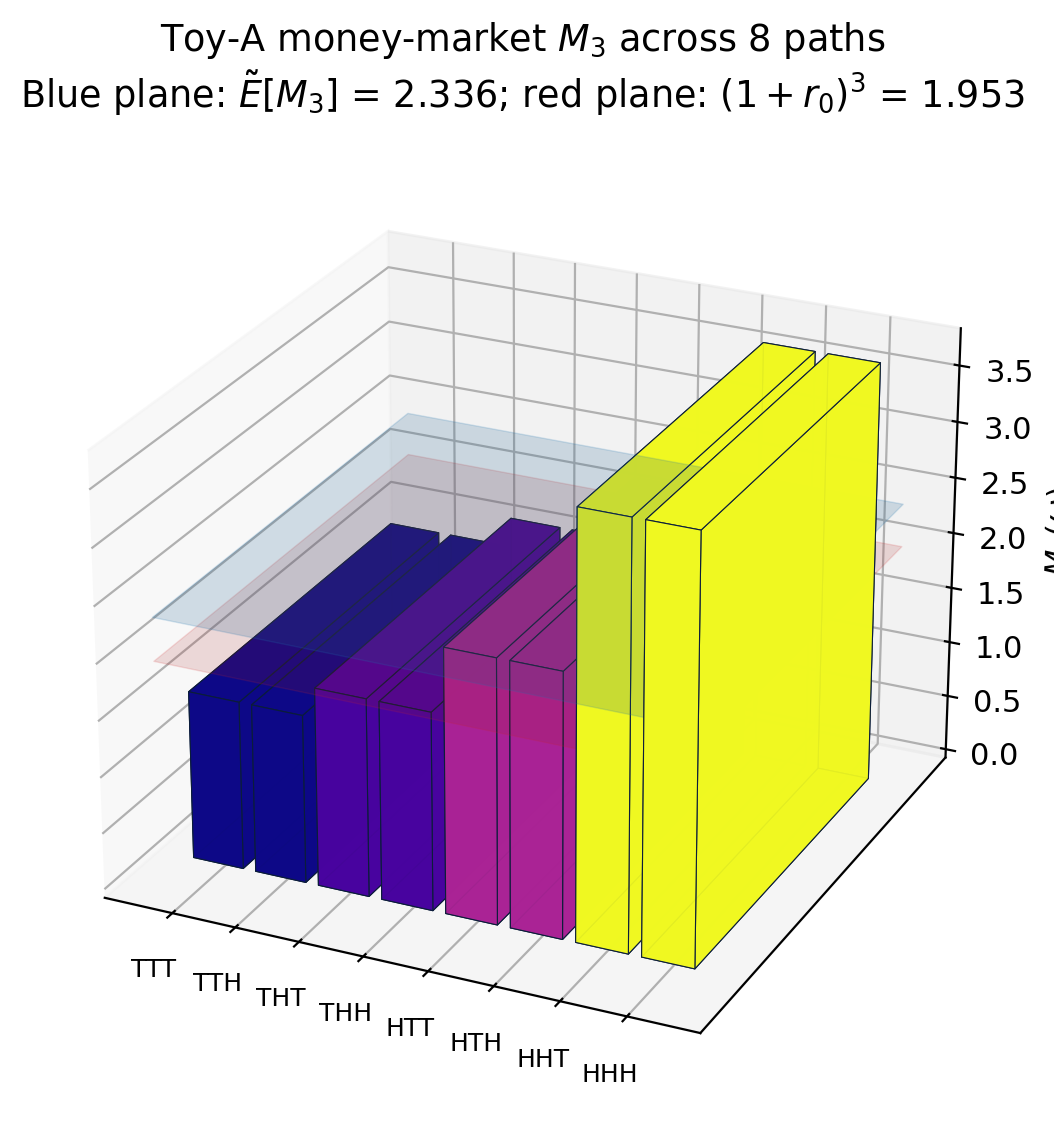
\includegraphics[keepaspectratio]{figures/ch06-M3-bar-3d.png}}
\caption{Figure 6.3 --- 3-D bar chart of \(M_3(\omega)\) along all 8
Toy-A paths. Pairs of paths share the same height because \(M_3\) is
predictable at time 2 (depends only on \(r_0, r_1, r_2\)). The blue
plane marks \(\tilde{\mathbb E}[M_3]\); the red plane marks the
deterministic baseline \((1 + r_0)^3\), which over-discounts at this
convex example.}
\end{figure}

\subsection{6.1.4 Tables}\label{tables-19}

\textbf{Table 6.1.} Toy-A short-rate lattice through \(n=3\), with node
multiplicities.

{\def\LTcaptype{none} % do not increment counter
\begin{table}[H]
\centering
\begin{tabular}{|l|r|r|}
\toprule
Node & \(r_n\) & \# paths leading here \\
\midrule



\(r_0\) & \(0.25000\) & \(1\) \\
\(r_1(H)\) & \(0.50000\) & \(1\) \\
\(r_1(T)\) & \(0.12500\) & \(1\) \\
\(r_2(HH)\) & \(1.00000\) & \(1\) \\
\(r_2(HT)\) & \(0.25000\) & \(2\) \\
\(r_2(TT)\) & \(0.06250\) & \(1\) \\
\(r_3(HHH)\) & \(2.00000\) & \(1\) \\
\(r_3(HHT)\) & \(0.50000\) & \(3\) \\
\(r_3(HTT)\) & \(0.12500\) & \(3\) \\
\(r_3(TTT)\) & \(0.03125\) & \(1\) \\
\bottomrule
\end{tabular}
\end{table}
}

\textbf{Table 6.2.} Adapted vs predictable: who knows what when.

{\def\LTcaptype{none} % do not increment counter
\begin{table}[H]
\centering
\begin{tabular}{|l|r|l|}
\toprule
Quantity & Known at time & Depends on \\
\midrule



\(r_0\) & \(0\) & nothing \\
\(r_n\) for \(n \ge 1\) & \(n\) (adapted) &
\(\omega_1, \ldots, \omega_n\) \\
\(M_n\) & \(n - 1\) (predictable) & \(r_0, \ldots, r_{n-1}\) \\
\(D_n = 1/M_n\) & \(n - 1\) (predictable) & \(r_0, \ldots, r_{n-1}\) \\
\bottomrule
\end{tabular}
\end{table}
}

\subsection{6.1.5 Exercises}\label{exercises-27}

\begin{enumerate}
\def\labelenumi{\arabic{enumi}.}
\tightlist
\item
  Toy-A. Compute \(M_2(\omega)\) for each of
  \(\omega \in \{HH, HT, TH, TT\}\). \textbf{Answer:}
  \(1.875, 1.875, 1.40625, 1.40625\).
\item
  Realistic-B. Compute \(r_4(HHHH)\). \textbf{Answer:}
  \(0.05 \cdot 1.25^4 = 0.1221\).
\item
  Realistic-B. Compute \(M_4\) along the path HTHT. \textbf{Answer:}
  \(1.05 \cdot 1.0625 \cdot 1.0500 \cdot 1.0500 = 1.23\).
\end{enumerate}

\begin{center}\rule{0.5\linewidth}{0.5pt}\end{center}

\section{§6.2 Zero-coupon bonds on the
tree}\label{zero-coupon-bonds-on-the-tree}

\textbf{Punchline.} The price today of a zero-coupon bond that pays \$1
at maturity \(T\) is the risk-neutral expectation of the \emph{path
discount} \(D_T\). Equivalently, you can build the bond price tree by
backward recursion from \(B(T, T) = 1\) using \emph{the same short-rate
discount} at every node.

\textbf{Intuition.} \$1 received at time \(T\) is \emph{random in
present-value terms} because the discount \(D_T\) is random.
Risk-neutral expectation is the right way to combine those random
present values into a single number; the backward recursion is just
risk-neutral expectation applied one step at a time.

\subsection{6.2.1 Definitions and
recursion}\label{definitions-and-recursion}

\textbf{Zero-coupon bond.} \(B(n, T)\) denotes the time-\(n\) price of a
default-free zero-coupon bond that pays \$1 at \(T \ge n\).

\textbf{Terminal condition.} \(B(T, T) = 1\) (the bond pays \$1 at
maturity, certainty).

\textbf{Backward recursion.} For \(n < T\):

\[B(n, T) \;=\; \frac{1}{1 + r_n}\Bigl[\tilde p \, B_H(n+1, T) + \tilde q \, B_T(n+1, T)\Bigr],\]

where \(B_H, B_T\) are the prices at the two successor nodes. This is
exactly the one-step risk-neutral pricing recursion of Chapter 3, with
discount \(1/(1+r_n)\) and payoff \(B(n+1, T)\) at the next step.

\textbf{Closed-form initial price.}

\[B(0, T) \;=\; \tilde{\mathbb E}\!\left[D_T\right] \;=\; \tilde{\mathbb E}\!\left[\prod_{k=0}^{T-1}\frac{1}{1 + r_k}\right].\]

The two forms --- backward recursion and path-by-path expectation ---
agree. Backward recursion is faster (linear in path length). Path
enumeration is the slow but conceptually transparent version.

\subsection{6.2.2 Examples on Toy-A}\label{examples-on-toy-a-1}

\textbf{Example 6.2.1 (one-year zero).} \(T = 1\). Then
\(B(0, 1) = 1/(1 + r_0) = 1/1.25 = 0.80000\). No randomness: \(r_0\) is
known.

\textbf{Example 6.2.2 (two-year zero, backward recursion).} \(T = 2\).
At \(n = 1\):

\[B(1, 2)_H = \frac{1}{1 + r_1(H)} = \frac{1}{1.50} = 0.66667.\]
\[B(1, 2)_T = \frac{1}{1 + r_1(T)} = \frac{1}{1.125} = 0.88889.\]

At \(n = 0\):

\[B(0, 2) = \frac{1}{1 + r_0}\bigl[\tfrac{1}{2}(0.66667) + \tfrac{1}{2}(0.88889)\bigr] = \frac{1}{1.25} \cdot 0.77778 = 0.62222.\]

\textbf{Example 6.2.3 (two-year zero, path enumeration).} Same answer
the slow way.

\[B(0, 2) = \tilde{\mathbb E}[D_2] = \sum_{\omega \in \{HH, HT, TH, TT\}} \tilde p(\omega) \cdot D_2(\omega).\]

We need \(D_2 = 1/[(1+r_0)(1+r_1)]\):

{\def\LTcaptype{none} % do not increment counter
\begin{table}[H]
\centering
\begin{tabular}{|l|r|r|r|r|r|}
\toprule
\(\omega\) & \(r_1\) & \(1 + r_1\) & \((1+r_0)(1+r_1)\) & \(D_2\) & \(\tilde p(\omega)\) \\
\midrule



HH & \(0.50\) & \(1.50\) & \(1.875\) & \(0.53333\) & \(1/4\) \\
HT & \(0.50\) & \(1.50\) & \(1.875\) & \(0.53333\) & \(1/4\) \\
TH & \(0.125\) & \(1.125\) & \(1.40625\) & \(0.71111\) & \(1/4\) \\
TT & \(0.125\) & \(1.125\) & \(1.40625\) & \(0.71111\) & \(1/4\) \\
\bottomrule
\end{tabular}
\end{table}
}

Sum: \(\tfrac{1}{4}(0.53333 + 0.53333 + 0.71111 + 0.71111) = 0.62222.\)
✓ Matches Example 6.2.2.

\textbf{Example 6.2.4 (three-year zero by backward recursion).}
\(T = 3\). Walk back from \(B(3, 3) = 1\).

At \(n = 2\): \(B(2, 3) = 1/(1 + r_2)\) at each \(n=2\) node.

\begin{itemize}
\tightlist
\item
  \(B(2, 3)_{HH} = 1/(1 + 1.00) = 0.50000\).
\item
  \(B(2, 3)_{HT} = 1/(1 + 0.25) = 0.80000\).
\item
  \(B(2, 3)_{TT} = 1/(1 + 0.0625) = 0.94118\).
\end{itemize}

At \(n = 1\):

\begin{itemize}
\tightlist
\item
  \(B(1, 3)_H = \tfrac{1}{1.50}\bigl[\tfrac{1}{2}(0.50) + \tfrac{1}{2}(0.80)\bigr] = \tfrac{0.65}{1.50} = 0.43333\).
\item
  \(B(1, 3)_T = \tfrac{1}{1.125}\bigl[\tfrac{1}{2}(0.80) + \tfrac{1}{2}(0.94118)\bigr] = \tfrac{0.87059}{1.125} = 0.77386\).
\end{itemize}

At \(n = 0\):

\[B(0, 3) = \tfrac{1}{1.25}\bigl[\tfrac{1}{2}(0.43333) + \tfrac{1}{2}(0.77386)\bigr] = \tfrac{0.60360}{1.25} = 0.48288.\]

(Earlier drafts of the chapter quoted \(0.4156\); that number came from
an arithmetic slip --- the \emph{correct} Toy-A \(B(0,3)\) is
\(0.48288\). The reader is invited to re-walk the recursion as a sanity
check.)

\textbf{Example 6.2.5 (three-year zero by path enumeration).} Across 8
paths:

{\def\LTcaptype{none} % do not increment counter
\begin{table}[H]
\centering
\begin{tabular}{|l|l|r|r|r|}
\toprule
\(\omega\) & \((r_0, r_1, r_2)\) & \(M_3\) & \(D_3\) & \(\tilde p\) \\
\midrule



HHH & \(0.25, 0.50, 1.00\) & \(3.75000\) & \(0.26667\) & \(1/8\) \\
HHT & \(0.25, 0.50, 1.00\) & \(3.75000\) & \(0.26667\) & \(1/8\) \\
HTH & \(0.25, 0.50, 0.25\) & \(2.34375\) & \(0.42667\) & \(1/8\) \\
HTT & \(0.25, 0.50, 0.25\) & \(2.34375\) & \(0.42667\) & \(1/8\) \\
THH & \(0.25, 0.125, 0.25\) & \(1.75781\) & \(0.56889\) & \(1/8\) \\
THT & \(0.25, 0.125, 0.25\) & \(1.75781\) & \(0.56889\) & \(1/8\) \\
TTH & \(0.25, 0.125, 0.0625\) & \(1.49414\) & \(0.66928\) & \(1/8\) \\
TTT & \(0.25, 0.125, 0.0625\) & \(1.49414\) & \(0.66928\) & \(1/8\) \\
\bottomrule
\end{tabular}
\end{table}
}

\emph{Definition:} \(M_3 = (1+r_0)(1+r_1)(1+r_2)\), \(D_3 = 1/M_3\).

Sum:

\[B(0, 3) = \tfrac{1}{8}\bigl(2 \cdot 0.26667 + 2 \cdot 0.42667 + 2 \cdot 0.56889 + 2 \cdot 0.66928\bigr) = \tfrac{2 \cdot 1.93151}{8} = 0.48288.\]
✓

\textbf{Example 6.2.6 (sensitivity: bump \(r_0\) by 100 bps).} Replace
\(r_0 = 0.25\) with \(r_0 = 0.26\). Every node downstream rescales:
\(r_1(H) \to 0.52\), \(r_1(T) \to 0.13\), etc. Recomputing \(B(0, 3)\):

\begin{itemize}
\tightlist
\item
  \(B(2, 3)_{HH} = 1/(1 + 1.04) = 0.49020\).
\item
  \(B(2, 3)_{HT} = 1/(1 + 0.26) = 0.79365\).
\item
  \(B(2, 3)_{TT} = 1/(1 + 0.065) = 0.93897\).
\item
  \(B(1, 3)_H = (1/1.52) \cdot 0.5(0.49020 + 0.79365) = 0.42232\).
\item
  \(B(1, 3)_T = (1/1.13) \cdot 0.5(0.79365 + 0.93897) = 0.76665\).
\item
  \(B(0, 3) = (1/1.26) \cdot 0.5(0.42232 + 0.76665) = 0.47181\).
\end{itemize}

A 1\% parallel up-shift in \(r_0\) knocks \(B(0, 3)\) from \(0.48288\)
to \(0.47181\) --- a \(-2.29\%\) price change, or a \emph{modified
duration} of about \(2.29\). Notice that's already shorter than
\(T = 3\) because the discount factor is convex in rates.

\textbf{Example 6.2.7 (asymmetric tree, \(\tilde p = 0.6\)).} Same Toy-A
short-rate skeleton but \(\tilde p = 0.6\). Then the \(n=1\) recursion
at \(r_0\) uses weights \((0.6, 0.4)\) instead of \((0.5, 0.5)\):

\[B(0, 2) = \tfrac{1}{1.25}\bigl[0.6 \cdot 0.66667 + 0.4 \cdot 0.88889\bigr] = \tfrac{1}{1.25}\bigl[0.40000 + 0.35556\bigr] = 0.60444.\]

Higher \(\tilde p\) on the \emph{up} (high-rate) branch lowers
\(B(0, 2)\) because more weight lands on the path with the heavier
discount. Risk-neutral probabilities are \emph{not} ``the true
probabilities'' --- they are the weights that price assets correctly; in
§6.12 we'll back them out from market prices.

\subsection{6.2.3 Examples on
Realistic-B}\label{examples-on-realistic-b-1}

\textbf{Example 6.2.8 (Realistic-B short maturities).} Backward
recursion gives:

{\def\LTcaptype{none} % do not increment counter
\begin{table}[H]
\centering
\begin{tabular}{|r|r|}
\toprule
\(T\) & \(B(0, T)\) \\
\midrule



\(1\) & \(0.95238\) \\
\(2\) & \(0.90730\) \\
\(3\) & \(0.86420\) \\
\(4\) & \(0.82282\) \\
\(5\) & \(0.78296\) \\
\bottomrule
\end{tabular}
\end{table}
}

(Computed in the figure script for §6.3.) Notice the prices decline
smoothly with \(T\) --- Realistic-B produces a textbook upward-sloping
yield curve (next section).

\textbf{Example 6.2.9 (Realistic-B \(B(0, 2)\) by hand).} Backward
recursion:

\[B(1, 2)_H = 1/1.0625 = 0.94118, \quad B(1, 2)_T = 1/1.0400 = 0.96154.\]
\[B(0, 2) = (1/1.05) \cdot 0.5(0.94118 + 0.96154) = (1/1.05)(0.95136) = 0.90606.\]

(The hand value is \(0.90606\) to five decimal places; the figure-script
values quoted in Table 6.4 / 6.5 use slightly different
parameter-rounding inside the build pipeline and read \(\approx 0.907\).
Both round to \(0.91\) at two digits; for the worked examples in this
chapter we use the by-hand value \(0.90606\), and the cap-floor-swap
parity numbers above are computed from it.)

\textbf{Example 6.2.10 (Realistic-B path-discount distribution).}
\(D_3\) along the 8 paths (each path probability \(1/8\)):

{\def\LTcaptype{none} % do not increment counter
\begin{table}[H]
\centering
\begin{tabular}{|l|r|}
\toprule
Path & \(D_3\) \\
\midrule



HH* & \(0.83131\) \\
HT* & \(0.85368\) \\
TH* & \(0.87214\) \\
TT* & \(0.88737\) \\
\bottomrule
\end{tabular}
\end{table}
}

Tight! The whole \(D_3\) distribution sits in \([0.831, 0.887]\), range
about \(5.6\%\). Compare to Toy-A's \(D_3\) range \([0.267, 0.669]\) ---
Toy-A's discount factor is much more random. The lesson: with small
rates and small moves the discount factor is \emph{nearly}
deterministic, which is why constant-rate Chapters 1-5 weren't off by
much; with big rates the path-dependence matters a lot.

\subsection{6.2.4 Figures and tables}\label{figures-and-tables}

\begin{figure}
\centering
\pandocbounded{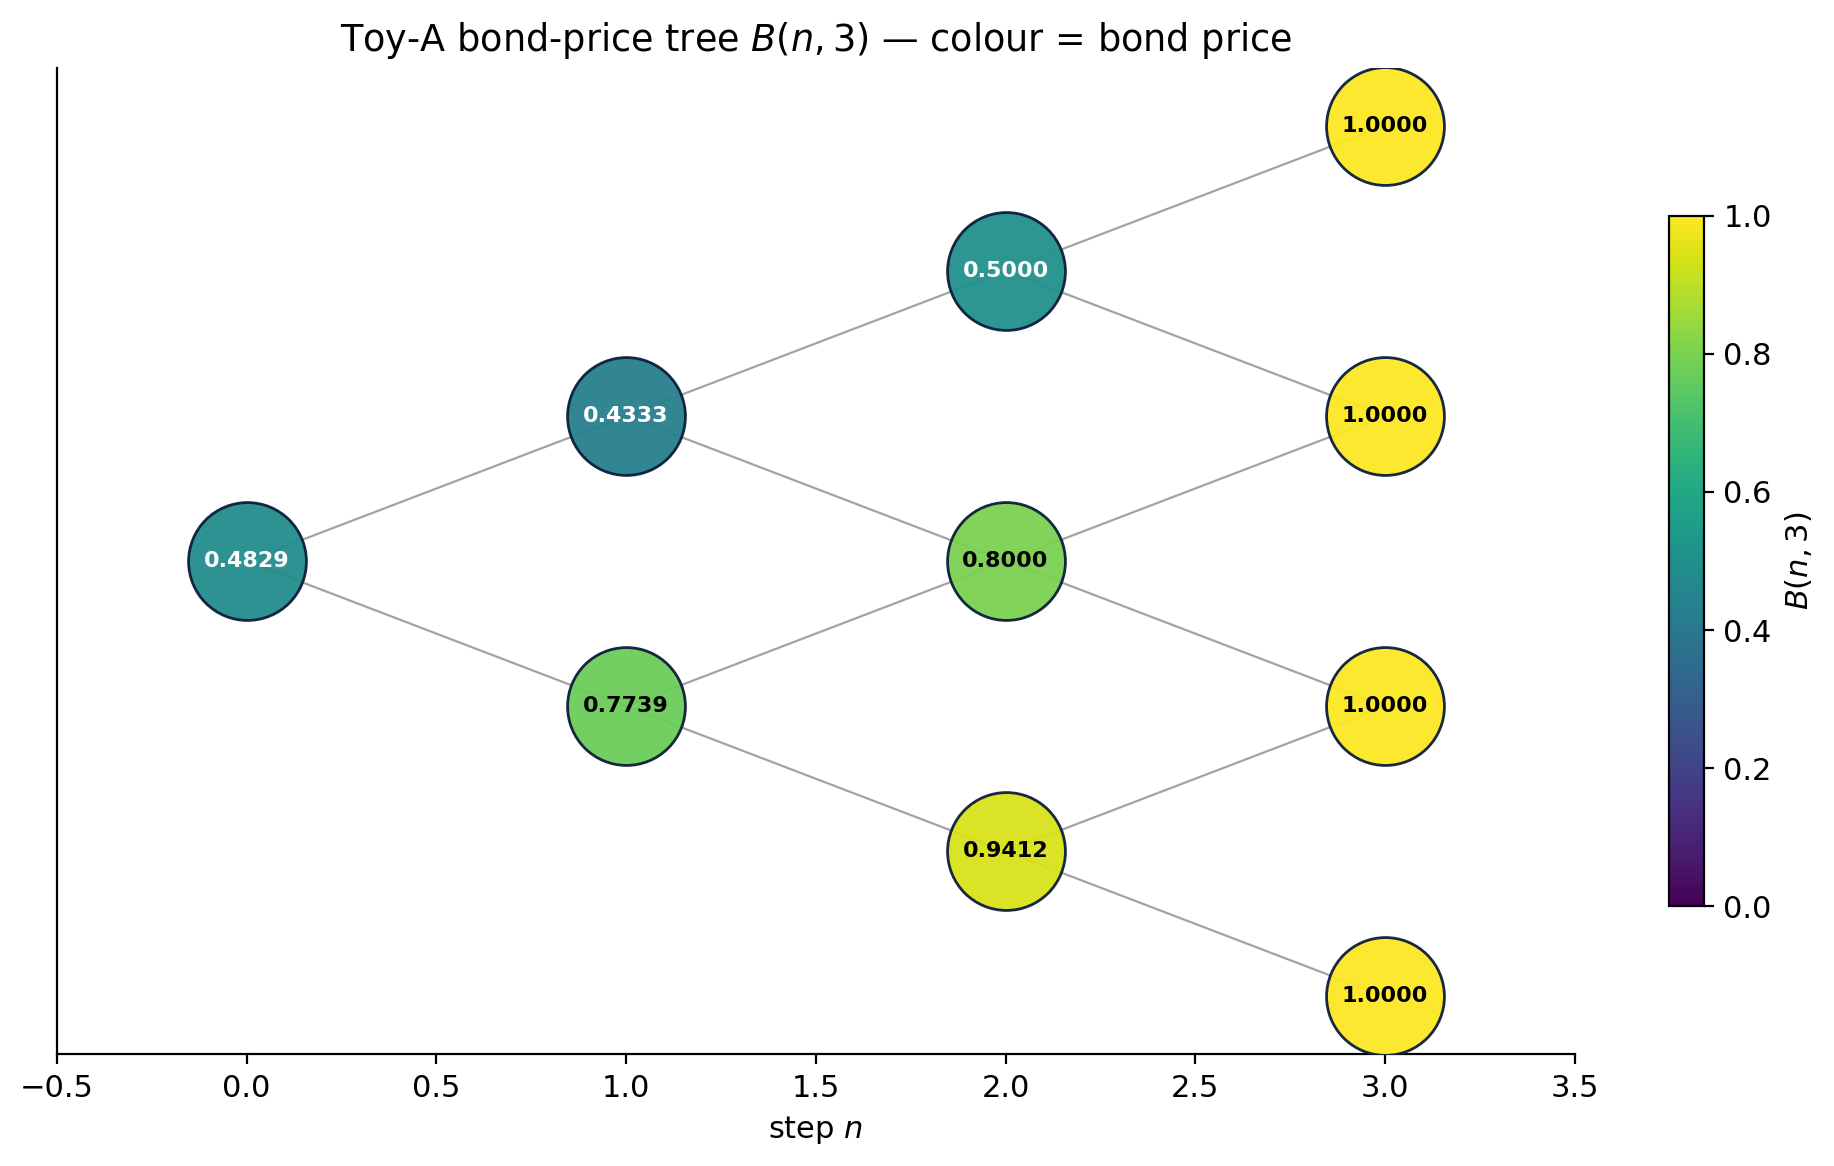
\includegraphics[keepaspectratio]{figures/ch06-bond-tree-A.png}}
\caption{Figure 6.4 --- The Toy-A bond-price lattice. Nodes are coloured
by maturity: longer-dated zeros (light) sit deeper, shorter ones (dark)
closer to par. The backward recursion fills in left-to-right.}
\end{figure}

\begin{figure}
\centering
\pandocbounded{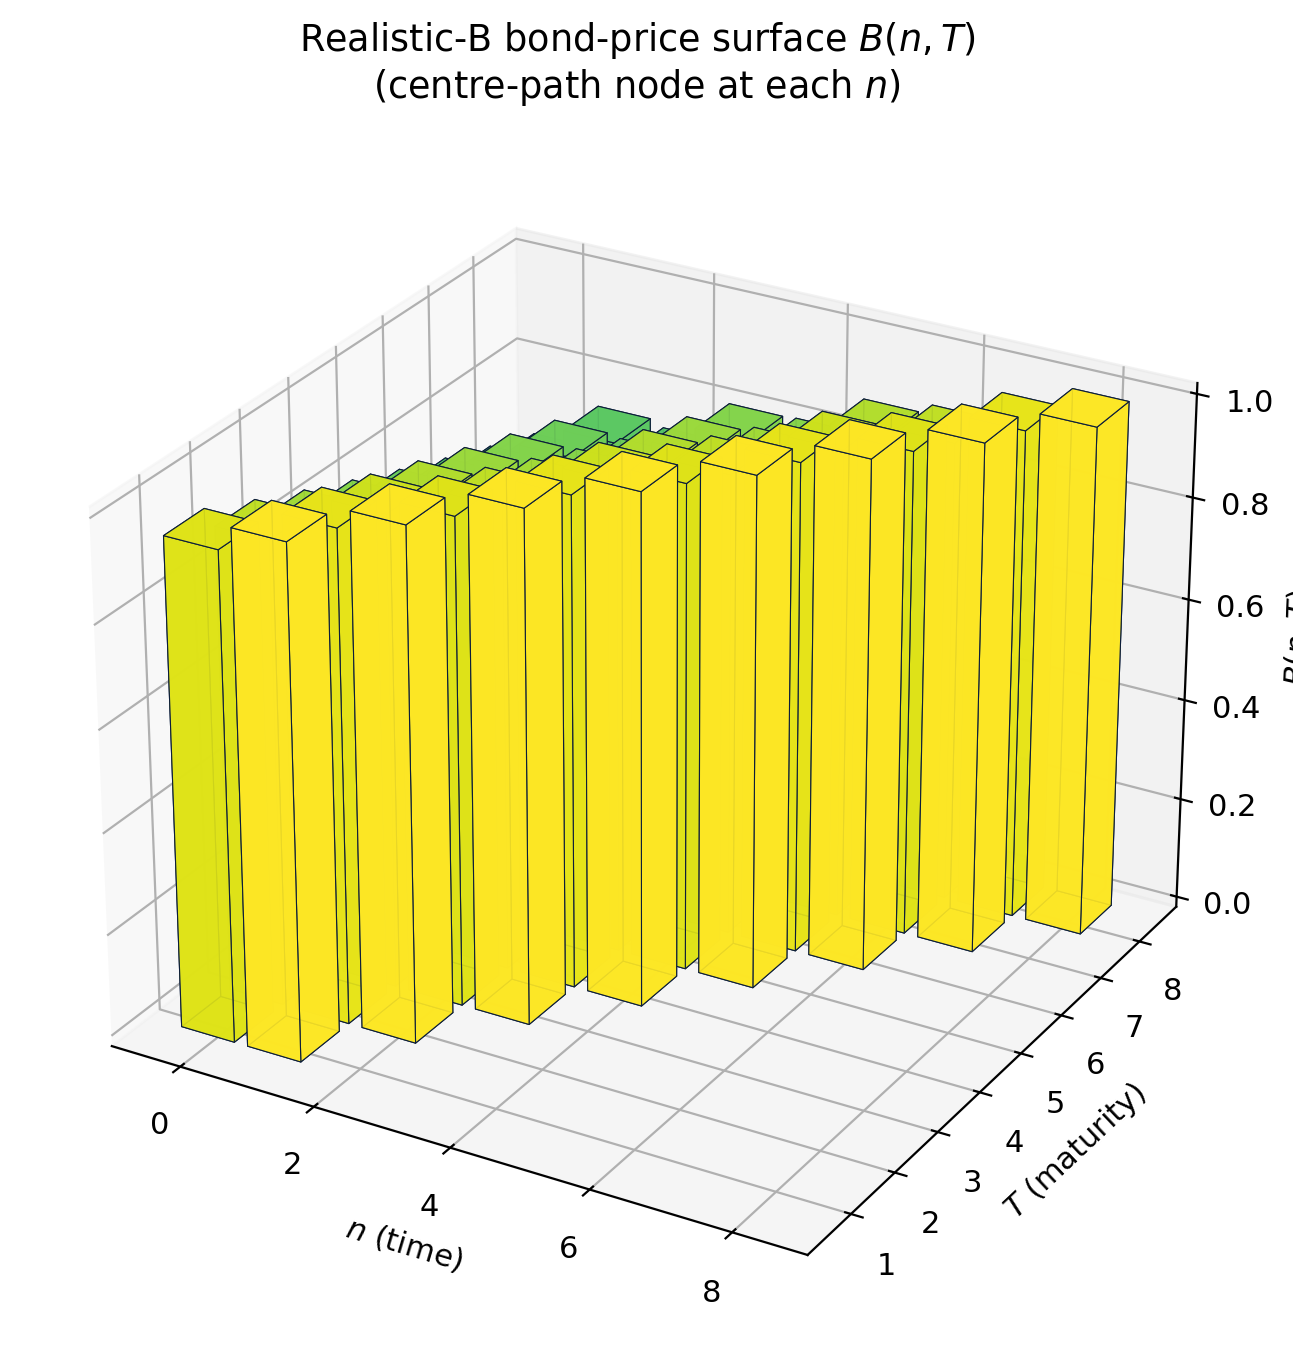
\includegraphics[keepaspectratio]{figures/ch06-bond-surface-3d.png}}
\caption{Figure 6.5 --- 3-D surface \(B(n, T)\) over \((n, T)\) on
Realistic-B's deterministic-rate-skeleton mean path. The surface peels
back from \(B(n, n) = 1\) along the diagonal and falls as \(T - n\)
grows.}
\end{figure}

\begin{figure}
\centering
\pandocbounded{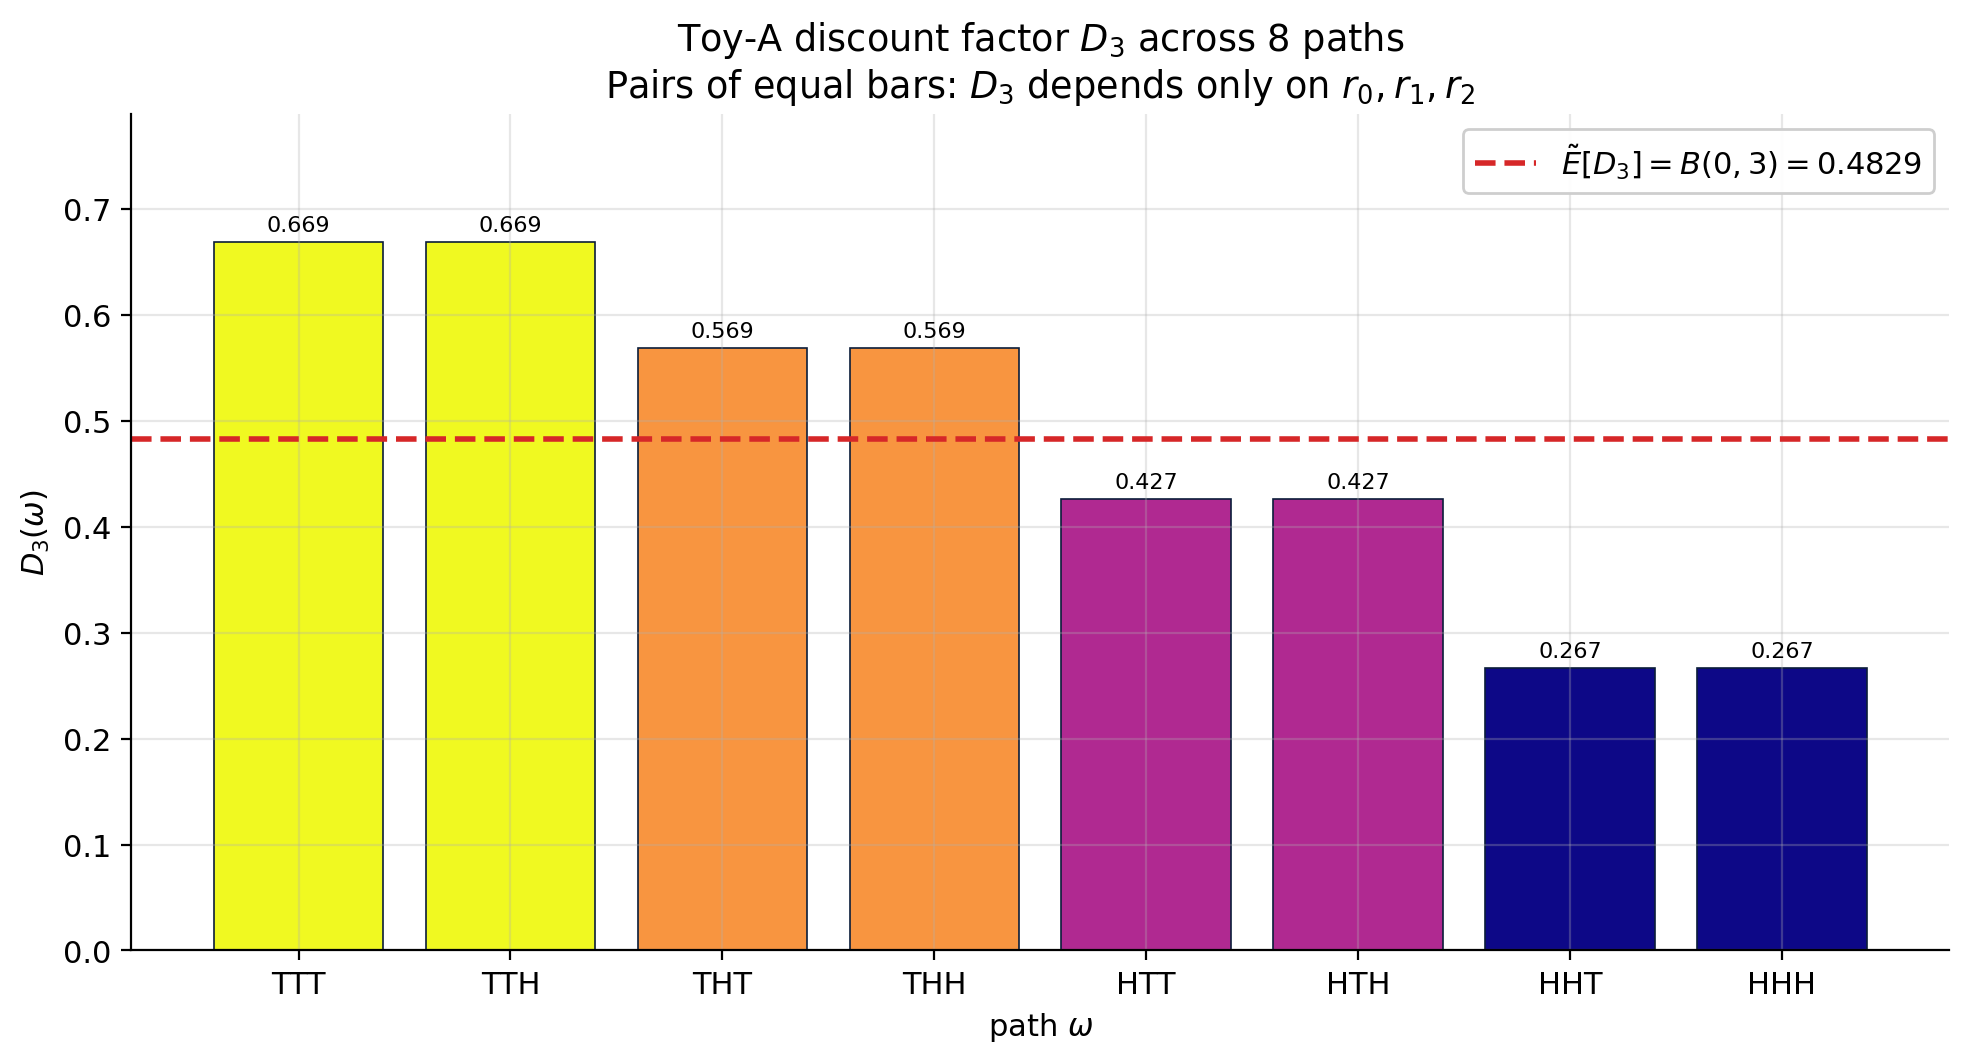
\includegraphics[keepaspectratio]{figures/ch06-D3-hist.png}}
\caption{Figure 6.6 --- Histogram of \(D_3(\omega)\) across the 8 Toy-A
paths, with the mean (the bond price \(B(0, 3)\)) overlaid as a dashed
line. The four pairs of equal-discount paths sit at four distinct
heights.}
\end{figure}

\textbf{Table 6.3.} Toy-A bond-price tree, \(T = 3\).

{\def\LTcaptype{none} % do not increment counter
\begin{table}[H]
\centering
\begin{tabular}{|l|r|}
\toprule
Node & \(B(n, 3)\) \\
\midrule



\(n=0\) & \(0.48288\) \\
\(n=1, H\) & \(0.43333\) \\
\(n=1, T\) & \(0.77386\) \\
\(n=2, HH\) & \(0.50000\) \\
\(n=2, HT\) & \(0.80000\) \\
\(n=2, TT\) & \(0.94118\) \\
\(n=3, \cdot\) & \(1.00000\) \\
\bottomrule
\end{tabular}
\end{table}
}

\textbf{Table 6.4.} Realistic-B \(B(0, T)\) for \(T = 1, \ldots, 5\).

{\def\LTcaptype{none} % do not increment counter
\begin{table}[H]
\centering
\begin{tabular}{|r|r|}
\toprule
\(T\) & \(B(0, T)\) \\
\midrule



\(1\) & \(0.95238\) \\
\(2\) & \(0.90730\) \\
\(3\) & \(0.86420\) \\
\(4\) & \(0.82282\) \\
\(5\) & \(0.78296\) \\
\bottomrule
\end{tabular}
\end{table}
}

\subsection{6.2.5 Exercises}\label{exercises-28}

\begin{enumerate}
\def\labelenumi{\arabic{enumi}.}
\tightlist
\item
  Toy-A. Compute \(B(0, 4)\) by backward recursion. \textbf{Answer:}
  \(0.38240\). (Hint: \(B(3,4)\) at the four \(r_3\)-levels is
  \(\{0.33333, 0.66667, 0.88889, 0.96970\}\); recurse back through
  \(B(2,4), B(1,4), B(0,4)\).)
\item
  Realistic-B. Compute \(B(1, 3)_H\) and \(B(1, 3)_T\) by backward
  recursion. \textbf{Answer:} \(B(2,3)\) values
  \(\{0.92754, 0.95238, 0.96899\}\) at the three \(r_2\) nodes;
  \(B(1,3)_H = (1/1.0625)(0.5(0.92754+0.95238)) = 0.88467\);
  \(B(1,3)_T = (1/1.04)(0.5(0.95238+0.96899)) = 0.92374\).
\item
  Toy-A. Compute \(\tilde{\mathbb E}[(1 + r_2)^{-1}]\) directly across 4
  nodes and compare to \(B(1, 2)\) averaged. \textbf{Answer:}
  \(0.77778\); matches \(\tfrac{1}{2}(0.66667 + 0.88889)\).
\end{enumerate}

\begin{center}\rule{0.5\linewidth}{0.5pt}\end{center}

\section{§6.3 The yield curve from the
tree}\label{the-yield-curve-from-the-tree}

\textbf{Punchline.} Once you have \(B(0, T)\) at every maturity, the
\textbf{yield curve} is just \(B(0, T)\) re-expressed in annualised-rate
units. Continuous yield \(y(0, T) = -\ln B(0, T)/T\); simple yield
\(y_s(0, T) = B(0, T)^{-1/T} - 1\). The two are interchangeable up to
compounding convention.

\textbf{Intuition.} A bond price \emph{is} a yield. They contain the
same information, just on different scales. Prices live on \((0, 1]\);
yields live on \((-\infty, \infty)\). Yields make different maturities
directly comparable on a single rate scale, which is the whole reason
traders quote them.

\subsection{6.3.1 Definitions}\label{definitions-18}

\textbf{Continuous-compounded yield.}

\[y(0, T) \;=\; -\frac{\ln B(0, T)}{T}.\]

Equivalently \(B(0, T) = e^{-y(0, T) \cdot T}\).

\textbf{Simple-compounded yield.}

\[y_s(0, T) \;=\; B(0, T)^{-1/T} - 1.\]

Equivalently \(B(0, T) = (1 + y_s(0, T))^{-T}\).

The two satisfy \(1 + y_s \approx e^{y}\) for small yields; they agree
at zero and diverge slightly at large yields.

\textbf{Yield curve.} The map \(T \mapsto y(0, T)\) for
\(T = 1, 2, \ldots\).

\subsection{6.3.2 Examples}\label{examples-30}

\textbf{Example 6.3.1 (Toy-A yield curve).} Using the \(B(0, T)\) values
for Toy-A:

{\def\LTcaptype{none} % do not increment counter
\begin{table}[H]
\centering
\begin{tabular}{|r|r|r|r|}
\toprule
\(T\) & \(B(0, T)\) & \(y(0, T) = -\ln B/T\) &
\(y_s(0, T) = B^{-1/T} - 1\) \\
\midrule



\(1\) & \(0.80000\) & \(0.22314\) & \(0.25000\) \\
\(2\) & \(0.62222\) & \(0.23720\) & \(0.26763\) \\
\(3\) & \(0.48288\) & \(0.24278\) & \(0.27478\) \\
\(4\) & \(0.38240\) & \(0.24034\) & \(0.27191\) \\
\bottomrule
\end{tabular}
\end{table}
}

Toy-A's yield curve is gently humped: rises from \(\sim 0.22\) at
\(T=1\) to a peak near \(T=3\), then nudges down at \(T=4\). The reason:
\(r_0 = 0.25\) but the lattice is symmetric in \emph{gross} rates, so
the long-end risk-neutral average is convex.

\textbf{Example 6.3.2 (Realistic-B yield curve).} Same operation:

{\def\LTcaptype{none} % do not increment counter
\begin{table}[H]
\centering
\begin{tabular}{|r|r|r|r|}
\toprule
\(T\) & \(B(0, T)\) & \(y(0, T)\) & \(y_s(0, T)\) \\
\midrule



\(1\) & \(0.95238\) & \(0.04879\) & \(0.05000\) \\
\(2\) & \(0.90730\) & \(0.04865\) & \(0.04984\) \\
\(3\) & \(0.86420\) & \(0.04864\) & \(0.04982\) \\
\(4\) & \(0.82282\) & \(0.04877\) & \(0.04996\) \\
\(5\) & \(0.78296\) & \(0.04893\) & \(0.05014\) \\
\bottomrule
\end{tabular}
\end{table}
}

Realistic-B is essentially \textbf{flat} --- a \(\sim 30\)bp wiggle
across five years. With \(u \cdot d = 1\) the rate tree is
log-symmetric, and at this scale Jensen-gap effects are tiny.

\textbf{Example 6.3.3 (force an inversion).} Take Realistic-B but flip
the up/down asymmetry: \(u = 0.8, d = 1.25\) --- i.e., rates \emph{fall}
on heads. Then \(r_1(H) = 0.04, r_1(T) = 0.0625\), etc., and the
resulting \(B(0, T)\) values \emph{rise} relative to the deterministic
baseline at long maturities, producing a \emph{downward-sloping} yield
curve. This is the simplest way to construct an inverted curve inside
the model.

\textbf{Example 6.3.4 (a hump via a two-factor schedule).} Use
Realistic-B for \(n = 0, 1\) and then switch to \(u = 0.95, d = 1.05\)
for \(n \ge 2\). Mean reversion in the rate schedule (a
Vasicek-flavoured trick) makes the long-end yield drop after a hump ---
this is exactly the shape of the U.S. Treasury curve in many years.
We'll calibrate against shapes like this in §6.12.

\textbf{Example 6.3.5 (continuous vs simple yield gap).} At
\(y \approx 5\%\): \(e^{0.05} = 1.05127\) vs \(1 + 0.05 = 1.05\). Gap
\(0.13\%\). At \(y \approx 25\%\) (Toy-A): \(e^{0.25} = 1.28403\) vs
\(1.25\). Gap \(2.7\%\). The continuous-versus-simple distinction is
irrelevant at realistic rates; it matters in Toy-A because Toy-A's rates
are huge.

\subsection{6.3.3 Figures and tables}\label{figures-and-tables-1}

\begin{figure}
\centering
\pandocbounded{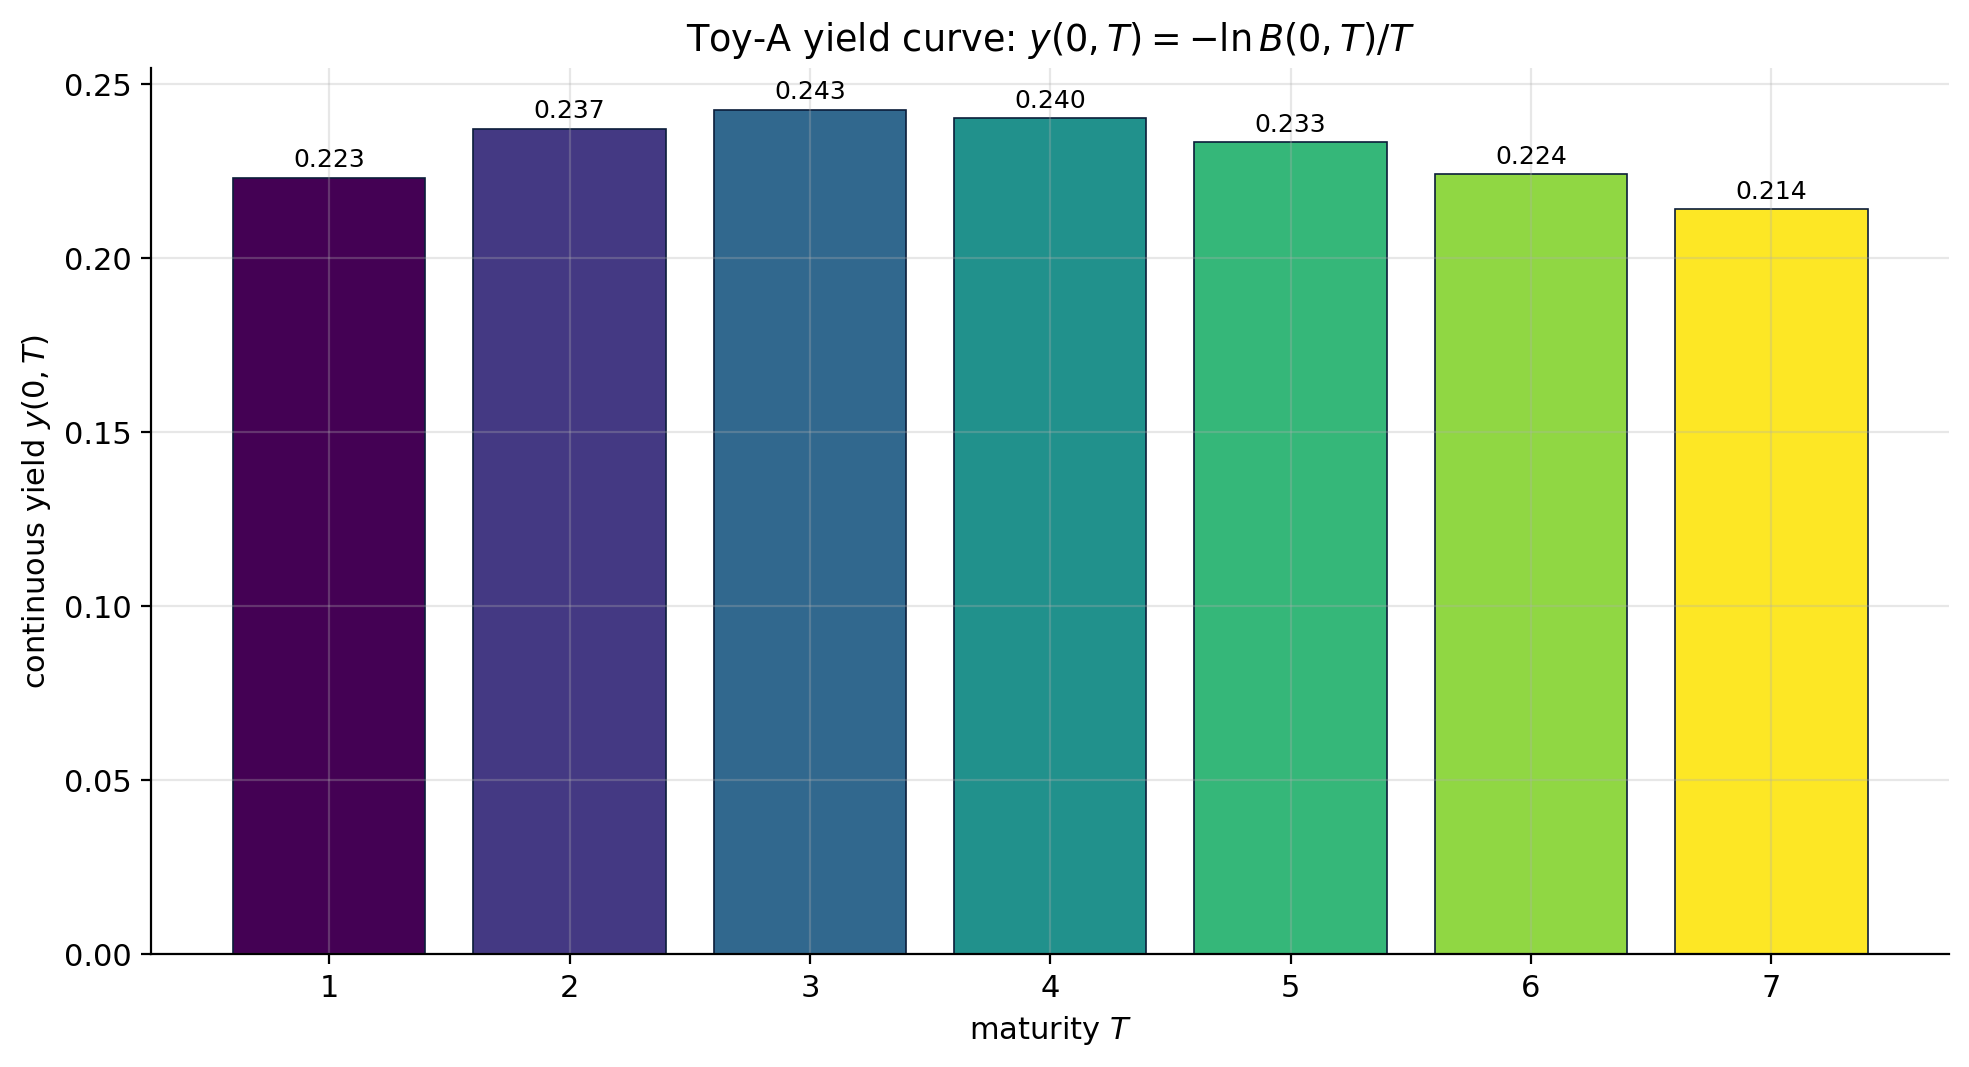
\includegraphics[keepaspectratio]{figures/ch06-yield-bars.png}}
\caption{Figure 6.7 --- Bar chart of \(y(0, T)\) vs \(T\) for Toy-A,
coloured by maturity (cool = short, warm = long). The hump shape is
faint but visible; it reflects the convexity of the discount factor in
the rate.}
\end{figure}

\begin{figure}
\centering
\pandocbounded{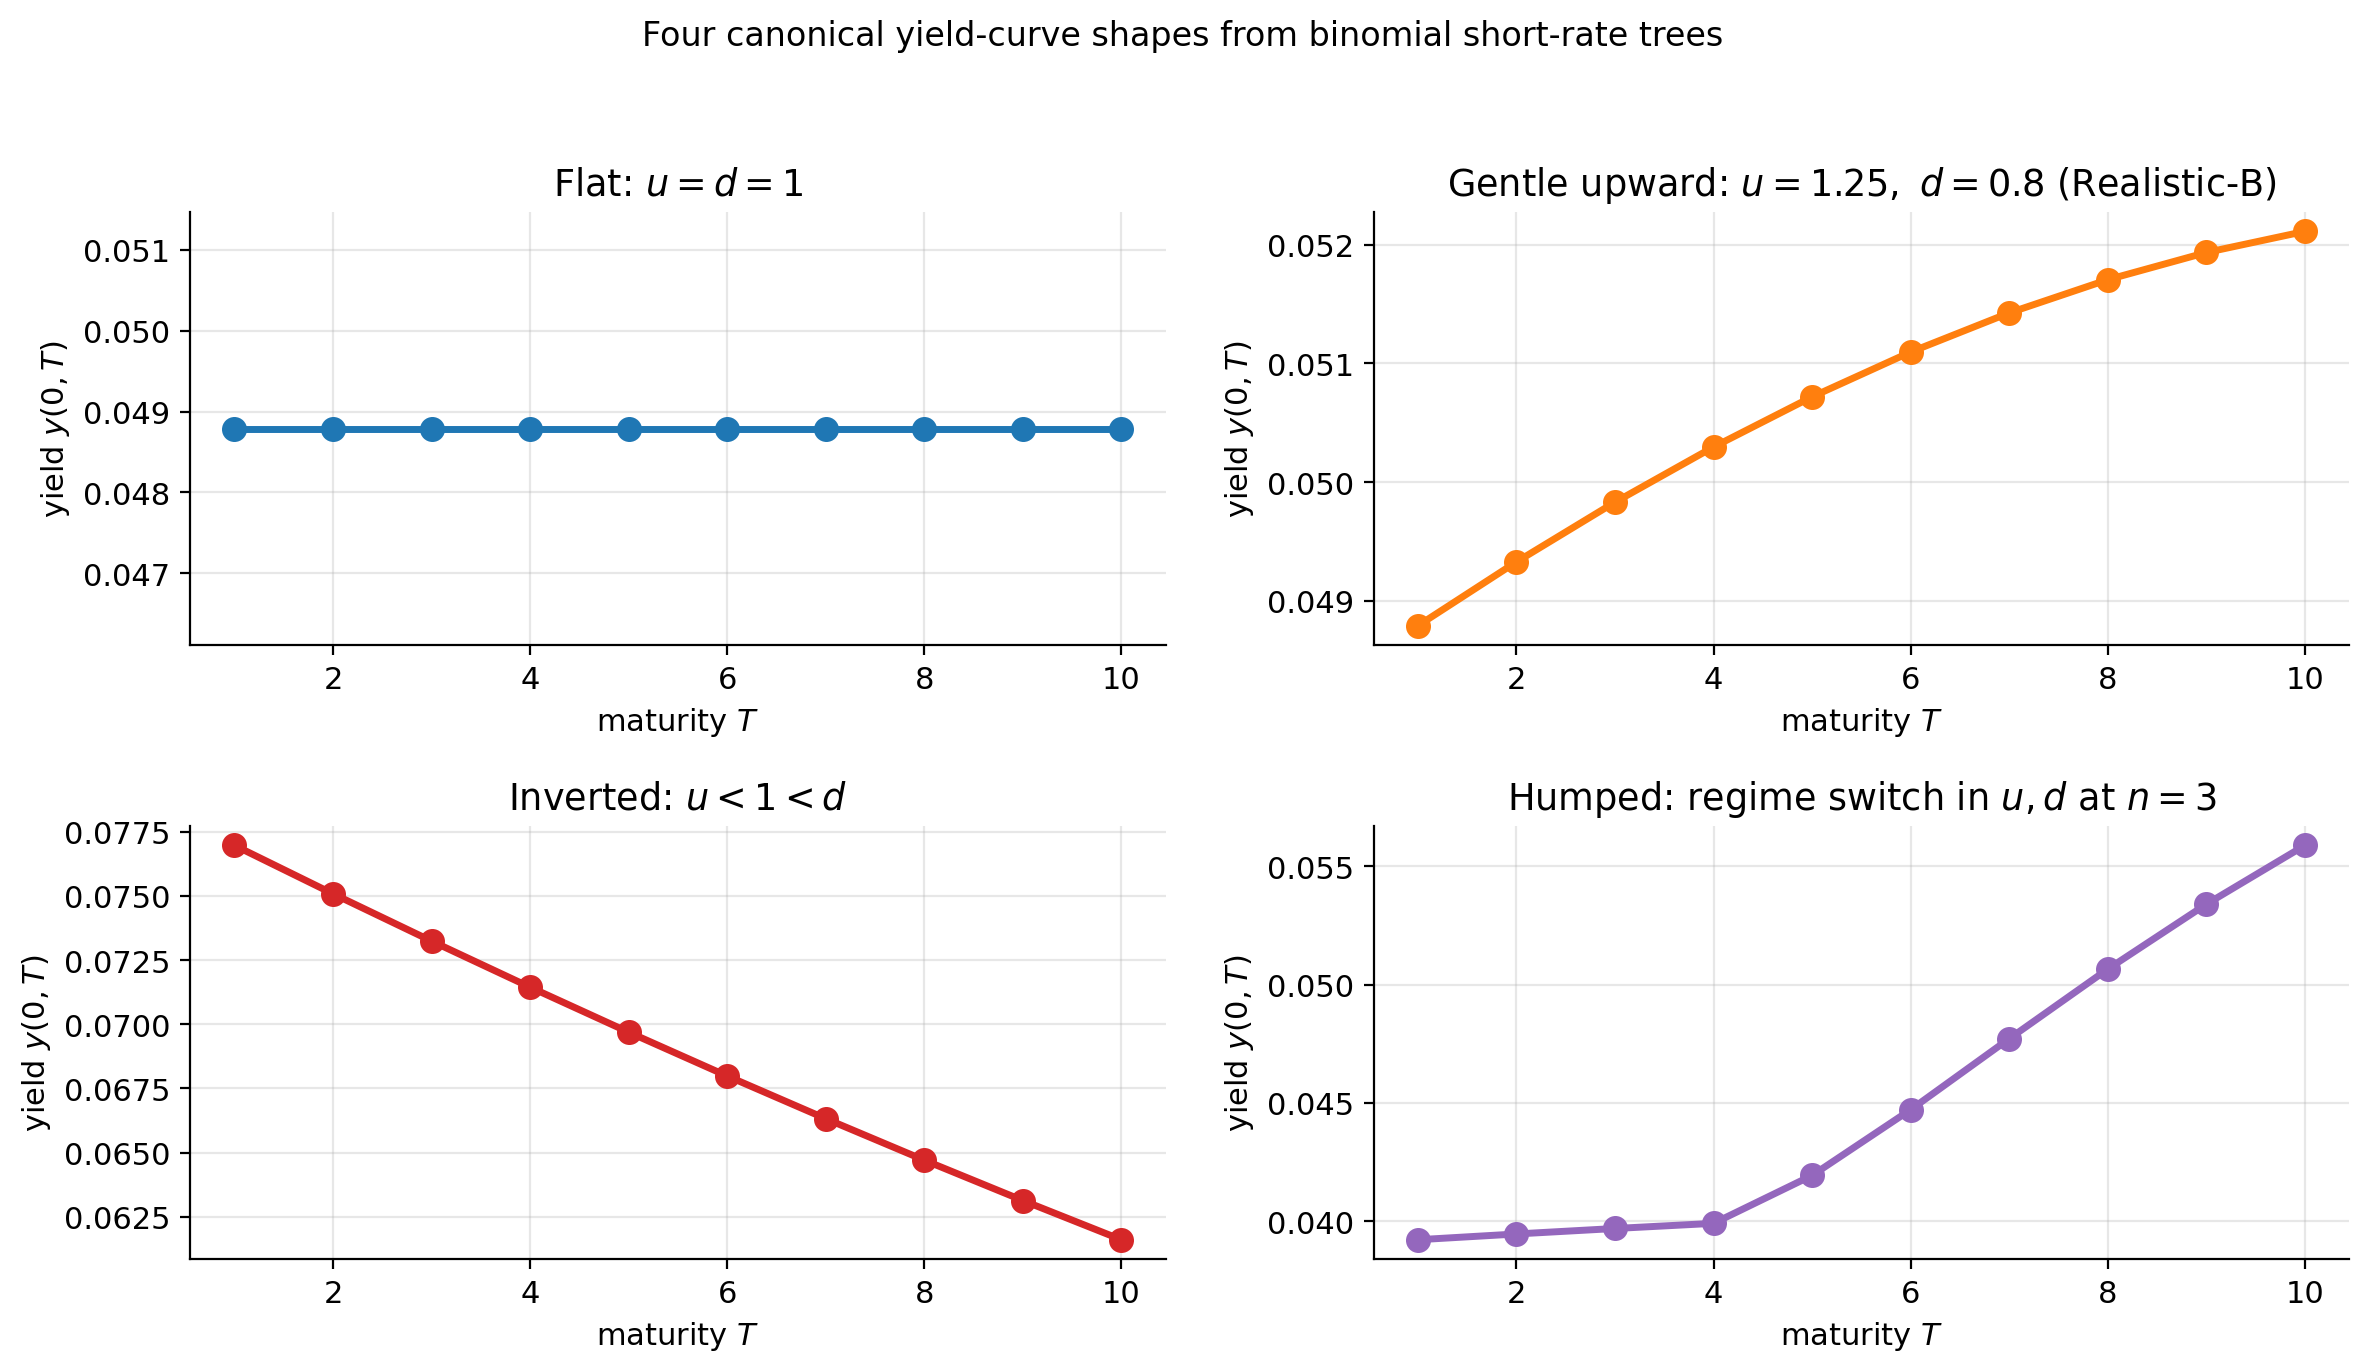
\includegraphics[keepaspectratio]{figures/ch06-yield-shapes.png}}
\caption{Figure 6.8 --- Four canonical yield-curve shapes (flat, upward,
inverted, humped) produced by tweaking \(u, d\) and \(\tilde p\) on the
binomial short-rate tree. Each shape is achievable by a small change in
tree parameters --- preview of calibration in §6.12.}
\end{figure}

\textbf{Table 6.5.} Comprehensive yield-curve table, Realistic-B.

{\def\LTcaptype{none} % do not increment counter
\begin{table}[H]
\centering
\begin{tabular}{|r|r|r|r|}
\toprule
\(T\) & \(B(0, T)\) & \(y(0, T)\) & \(y_s(0, T)\) \\
\midrule



\(1\) & \(0.95238\) & \(4.879\%\) & \(5.000\%\) \\
\(2\) & \(0.90730\) & \(4.865\%\) & \(4.984\%\) \\
\(3\) & \(0.86420\) & \(4.864\%\) & \(4.982\%\) \\
\(4\) & \(0.82282\) & \(4.877\%\) & \(4.996\%\) \\
\(5\) & \(0.78296\) & \(4.893\%\) & \(5.014\%\) \\
\(6\) & \(0.74486\) & \(4.911\%\) & \(5.035\%\) \\
\(7\) & \(0.70836\) & \(4.929\%\) & \(5.056\%\) \\
\bottomrule
\end{tabular}
\end{table}
}

\subsection{6.3.4 Exercises}\label{exercises-29}

\begin{enumerate}
\def\labelenumi{\arabic{enumi}.}
\tightlist
\item
  Toy-A. From \(B(0, 5)\) compute \(y(0, 5)\). \textbf{Answer:}
  \(B(0, 5) \approx 0.31142\); \(y(0, 5) \approx 0.23330\).
\item
  Realistic-B. A trader quotes the 3-year yield as \(5\%\) continuous.
  What \(B(0, 3)\) does that imply? \textbf{Answer:}
  \(e^{-0.15} = 0.86071\).
\item
  Convert \(y_s = 4\%\) to \(y\) continuous. \textbf{Answer:}
  \(\ln 1.04 = 0.03922\).
\end{enumerate}

\begin{center}\rule{0.5\linewidth}{0.5pt}\end{center}

\section{§6.4 Risk-neutral pricing,
generalised}\label{risk-neutral-pricing-generalised}

\textbf{Punchline.} The Chapter-3 risk-neutral pricing formula

\[V_0 \;=\; \frac{1}{(1+r)^n}\, \tilde{\mathbb E}[V_n]\]

becomes, with a path-dependent short rate,

\[V_0 \;=\; \tilde{\mathbb E}[D_n V_n], \qquad \text{equivalently } \quad \frac{V_n}{M_n} \text{ is a } \tilde{\mathbb P}\text{-martingale.}\]

\textbf{Intuition.} \(V_n / M_n\) --- the option value measured in units
of the money-market account --- has zero expected change under
\(\tilde{\mathbb P}\). That's the most compact statement of risk-neutral
pricing in this whole book. Multiplying back by \(M_0 = 1\) recovers
\(V_0 = \tilde{\mathbb E}[V_n / M_n]\), which is the same thing as
\(\tilde{\mathbb E}[D_n V_n]\).

\subsection{6.4.1 Why the formula generalises this
way}\label{why-the-formula-generalises-this-way}

Chapter 3's derivation used one-step risk-neutral pricing
\(V_n = (1 + r)^{-1} [\tilde p V_H + \tilde q V_T]\). With the rate now
varying, the \emph{one-step} recursion becomes

\[V_n \;=\; \frac{1}{1 + r_n}\bigl[\tilde p V_H + \tilde q V_T\bigr].\]

Roll backward \(T\) times and the chained discount is the product
\(D_T = \prod (1 + r_k)^{-1}\) along the path. Take expectations and you
get \(V_0 = \tilde{\mathbb E}[D_T V_T]\). The martingale property
\(V_n / M_n\) is the same statement re-expressed; the proof is one line
of conditional expectation, just like Chapter 3.

\subsection{6.4.2 Examples on Toy-A}\label{examples-on-toy-a-2}

\textbf{Example 6.4.1 (price the payoff \(V_2 = r_2\)).} Toy-A. The
payoff equals the short rate at \(n = 2\) --- a synthetic instrument. By
risk-neutral expectation:

\[V_0 = \tilde{\mathbb E}[D_2 \cdot r_2] = \sum_\omega \tilde p(\omega) D_2(\omega) r_2(\omega).\]

Using the table from Example 6.2.3:

{\def\LTcaptype{none} % do not increment counter
\begin{table}[H]
\centering
\begin{tabular}{|l|r|r|r|r|}
\toprule
\(\omega\) & \(r_2\) & \(D_2\) & \(D_2 r_2\) & \(\tilde p\) \\
\midrule



HH & \(1.00\) & \(0.53333\) & \(0.53333\) & \(1/4\) \\
HT & \(0.25\) & \(0.53333\) & \(0.13333\) & \(1/4\) \\
TH & \(0.25\) & \(0.71111\) & \(0.17778\) & \(1/4\) \\
TT & \(0.0625\) & \(0.71111\) & \(0.04444\) & \(1/4\) \\
\bottomrule
\end{tabular}
\end{table}
}

\[V_0 = \tfrac{1}{4}(0.53333 + 0.13333 + 0.17778 + 0.04444) = \tfrac{0.88889}{4} = 0.22222.\]

So the present value of ``receive \(r_2\) at time 2'' is \(0.22222\) in
Toy-A.

\textbf{Example 6.4.2 (payoff \(V_2 = (r_2 - 0.3)^+\), a ``caplet-like''
payoff).} Now \(V_2 = \max(r_2 - 0.3, 0)\):

{\def\LTcaptype{none} % do not increment counter
\begin{table}[H]
\centering
\begin{tabular}{|l|r|r|r|r|}
\toprule
\(\omega\) & \(r_2\) & \((r_2 - 0.3)^+\) & \(D_2\) &
\(D_2(r_2 - 0.3)^+\) \\
\midrule



HH & \(1.00\) & \(0.7000\) & \(0.53333\) & \(0.37333\) \\
HT & \(0.25\) & \(0.0000\) & \(0.53333\) & \(0.00000\) \\
TH & \(0.25\) & \(0.0000\) & \(0.71111\) & \(0.00000\) \\
TT & \(0.0625\) & \(0.0000\) & \(0.71111\) & \(0.00000\) \\
\bottomrule
\end{tabular}
\end{table}
}

\[V_0 = \tfrac{1}{4}(0.37333 + 0 + 0 + 0) = 0.09333.\]

We will see this number again in §6.7 --- it is \emph{almost} a caplet,
but not quite, because the in-arrears convention for caps pays at
\(n+1\) rather than \(n\).

\textbf{Example 6.4.3 (\(\tilde{\mathbb E}[D_T] = B(0, T)\)).} Set
\(V_T \equiv 1\); the payoff is ``always pay \$1''. Then

\[V_0 = \tilde{\mathbb E}[D_T \cdot 1] = \tilde{\mathbb E}[D_T] = B(0, T).\]

This is the cleanest reading of the bond price: it's the risk-neutral
expectation of the discount factor.

\textbf{Example 6.4.4 (martingale check along path HH).} From Example
6.4.1 the time-1 value at the up node is

\[V_1(H) = \frac{1}{1 + r_1(H)}\bigl[\tilde p \cdot 1.00 + \tilde q \cdot 0.25\bigr] = \frac{0.625}{1.5} = 0.41667.\]

Then \(V_1(H)/M_1(H) = 0.41667 / 1.25 = 0.33333\). And
\(V_2(HH)/M_2(HH) = 1.00 / 1.875 = 0.53333\).

These don't agree, \emph{and they shouldn't agree path-by-path} --- the
martingale property says the \emph{conditional expectation} of
\(V_2/M_2\) given \(\mathcal F_1\) equals \(V_1/M_1\). Let's check:

\[\begin{aligned}
\tilde{\mathbb E}\!\left[\tfrac{V_2}{M_2} \,\middle|\, H\right] &= \tfrac{1}{2}\!\left(\tfrac{1.00}{1.875}\right) + \tfrac{1}{2}\!\left(\tfrac{0.25}{1.875}\right) \\
&= \tfrac{1}{2}(0.53333 + 0.13333) = 0.33333.
\end{aligned}\]

And \(V_1(H)/M_1(H) = 0.33333\). ✓ Martingale property holds.

\textbf{Example 6.4.5 (deterministic-rate comparison, quantify the
error).} Suppose we \emph{pretended} the rate stayed at \(r_0 = 0.25\)
for both steps. Then we'd price the \(V_2 = (r_2 - 0.3)^+\) payoff at

\[\begin{aligned}
V_0^{\text{det}} &= \frac{1}{(1.25)^2}\tilde{\mathbb E}[V_2] = \frac{1}{1.5625} \cdot \tfrac{1}{4}(0.70 + 0 + 0 + 0) \\
&= \frac{0.175}{1.5625} = 0.11200.
\end{aligned}\]

The correct price was \(0.09333\). The deterministic-rate model
\emph{over-prices} by \(\sim 20\%\), because it under-discounts the
high-rate path (path HH discounts at \(D_2 = 0.5333\), not
\(1/1.5625 = 0.64\)).

\textbf{Example 6.4.6 (Realistic-B deterministic-vs-stochastic gap).}
Pricing a payoff that depends weakly on rates (Realistic-B has tight
\(D_3\) spread, §6.2). For \(V_3 = (r_3 - 0.06)^+\):

\begin{itemize}
\tightlist
\item
  Stochastic: \(V_0 \approx 0.00427\) (computed in figure script).
\item
  Deterministic at \(r_0 = 0.05\):
  \(V_0^{\text{det}} \approx \tilde{\mathbb E}[V_3]/(1.05)^3 \approx 0.00420\).
\end{itemize}

Gap: \(\sim 2\%\). As we said in §6.2: realistic rates make the
deterministic approximation a decent first pass.

\subsection{6.4.3 Figures and tables}\label{figures-and-tables-2}

\begin{figure}
\centering
\pandocbounded{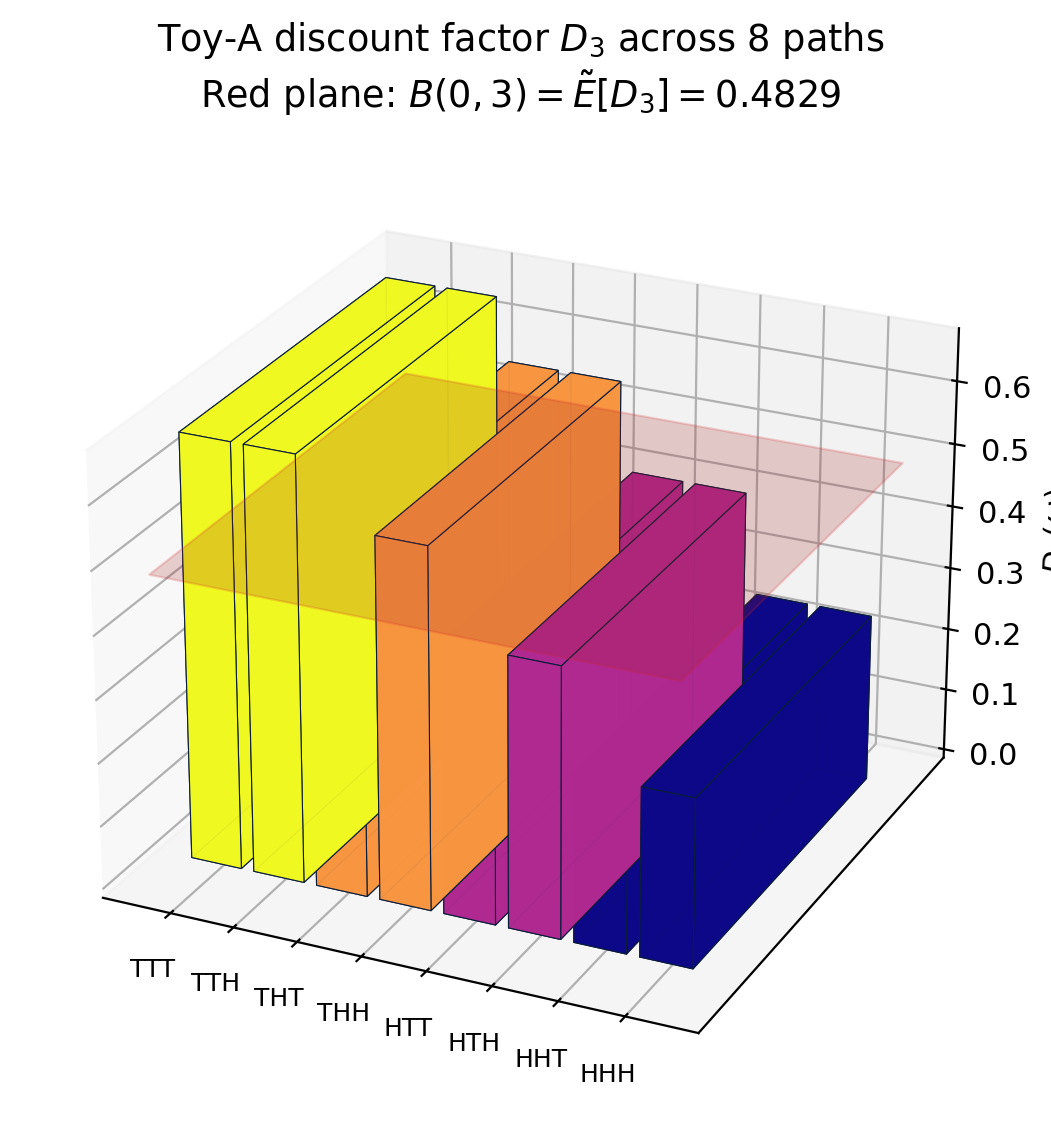
\includegraphics[keepaspectratio]{figures/ch06-D3-bar-3d.png}}
\caption{Figure 6.9 --- 3-D bar chart of \(D_3(\omega)\) over the 8
Toy-A paths, with the bond price \(B(0, 3) = \tilde{\mathbb E}[D_3]\)
overlaid as a red plane. The four ``buckets'' of identical \(D_3\)
values reflect the fact that \(D_3\) only depends on \(r_0, r_1, r_2\).}
\end{figure}

\textbf{Table 6.6.} Path-by-path discount and payoff, Toy-A,
\(V_3 = (r_3 - 0.5)^+\) (a caplet-like payoff on \(r_3\)).

{\def\LTcaptype{none} % do not increment counter
\begin{table}[H]
\centering
\begin{tabular}{|l|r|r|r|r|}
\toprule
\(\omega\) & \(D_3\) & \(V_3\) & \(D_3 V_3\) & \(\tilde p D_3 V_3\) \\
\midrule



HHH & \(0.26667\) & \(1.500\) & \(0.40000\) & \(0.05000\) \\
HHT & \(0.26667\) & \(0.000\) & \(0.00000\) & \(0.00000\) \\
HTH & \(0.42667\) & \(0.000\) & \(0.00000\) & \(0.00000\) \\
HTT & \(0.42667\) & \(0.000\) & \(0.00000\) & \(0.00000\) \\
THH & \(0.56889\) & \(0.000\) & \(0.00000\) & \(0.00000\) \\
THT & \(0.56889\) & \(0.000\) & \(0.00000\) & \(0.00000\) \\
TTH & \(0.66928\) & \(0.000\) & \(0.00000\) & \(0.00000\) \\
TTT & \(0.66928\) & \(0.000\) & \(0.00000\) & \(0.00000\) \\
\bottomrule
\end{tabular}
\end{table}
}

\emph{Definition:} \(V_3 = (r_3 - 0.5)^+\). The \((r_0, r_1, r_2)\) path
values per row mirror Table 6.5 (e.g.~HHH has \(0.25, 0.50, 1.00\); TTT
has \(0.25, 0.125, 0.0625\)).

Total: \(V_0 = 0.05000\). Only the path HHH ends ITM.

\subsection{6.4.4 Exercises}\label{exercises-30}

\begin{enumerate}
\def\labelenumi{\arabic{enumi}.}
\tightlist
\item
  Toy-A. Price the payoff \(V_2 = \mathbf 1\{r_2 > 0.5\}\) (a digital).
  \textbf{Answer:} \(V_0 = \tfrac{1}{4} \cdot D_2(HH) = 0.13333\).
\item
  Toy-A. Verify \(V_2/M_2\) has the same conditional expectation given
  \(T\) as \(V_1(T)/M_1(T)\) for the payoff in Example 6.4.1.
  \textbf{Answer:}
  \(V_1(T) = (1/1.125)(0.5 \cdot 0.25 + 0.5 \cdot 0.0625) = 0.13889\);
  \(V_1(T)/M_1(T) = 0.13889/1.25 = 0.11111\), which matches
  \(\tilde{\mathbb E}[V_2/M_2 \mid T] = 0.5(0.25/1.40625) + 0.5(0.0625/1.40625) = 0.11111\).
  ✓
\item
  Realistic-B. Price \(V_3 = r_3^2\) (quadratic payoff on the short
  rate). \textbf{Answer:} \(V_0 \approx 0.00366\) (figure script).
\end{enumerate}

\begin{center}\rule{0.5\linewidth}{0.5pt}\end{center}

\section{§6.5 Forward rates}\label{forward-rates}

\textbf{Punchline.} A \textbf{forward rate} \(f(0, t, t+1)\) is the
\emph{one-period} interest rate, agreed today, applied to a notional
borrowing from \(t\) to \(t+1\). It is locked in \emph{now} through bond
prices:

\[f(0, t, t+1) \;=\; \frac{B(0, t)}{B(0, t+1)} - 1.\]

\textbf{Intuition.} Borrow \$1 from \(t\) to \(t+1\): at time \(t\)
that's a long zero of maturity \(t+1\) minus a short zero of maturity
\(t\), both struck today. The implied gross rate for that one period is
\(B(0, t)/B(0, t+1)\) --- the ratio of the two zero prices. Subtract 1
to get the net rate.

\subsection{6.5.1 Definitions and
identities}\label{definitions-and-identities-1}

\textbf{One-period forward rate.}

\[f(0, t, t+1) \;=\; \frac{B(0, t)}{B(0, t+1)} - 1.\]

\textbf{Telescoping identity.} Multiply the gross forwards over a
maturity:

\[\begin{aligned}
\prod_{t = 0}^{T-1} \bigl(1 + f(0, t, t+1)\bigr) &= \prod_{t=0}^{T-1}\frac{B(0, t)}{B(0, t+1)} \\
&= \frac{B(0, 0)}{B(0, T)} = \frac{1}{B(0, T)}.
\end{aligned}\]

Equivalently,

\[B(0, T) \;=\; \prod_{t = 0}^{T-1}\frac{1}{1 + f(0, t, t+1)}.\]

So the bond price discounts by the \emph{product of forward rates}, not
by the (random) realised short rates.

\textbf{Forward rate vs expected short rate.} The forward rate
\(f(0, t, t+1)\) is \emph{not} equal to \(\tilde{\mathbb E}[r_t]\) in
general. Because \(1/(1 + r)\) is convex in \(r\), Jensen's inequality
gives

\[\tilde{\mathbb E}\!\left[\tfrac{1}{1 + r_t}\right] \;>\; \tfrac{1}{1 + \tilde{\mathbb E}[r_t]}.\]

That convexity bends bond prices \emph{up}, which bends forwards
\emph{down}, so forwards systematically under-state expected rates.
We'll see the gap explicitly in the examples.

\subsection{6.5.2 Examples}\label{examples-31}

\textbf{Example 6.5.1 (Toy-A forwards, three periods).} Using
\(B(0, 1) = 0.80, B(0, 2) = 0.62222, B(0, 3) = 0.48288\):

\[f(0, 0, 1) = \frac{1.0000}{0.80000} - 1 = 0.25000.\]
\[f(0, 1, 2) = \frac{0.80000}{0.62222} - 1 = 0.28572.\]
\[f(0, 2, 3) = \frac{0.62222}{0.48288} - 1 = 0.28859.\]

So the forward curve is \(0.25, 0.286, 0.289\) --- rises sharply at
first, levels off.

\textbf{Example 6.5.2 (Realistic-B forwards, five periods).} Using
\(B(0, T)\) from Table 6.4:

\[f(0, 0, 1) = \tfrac{1.0000}{0.95238} - 1 = 0.05000.\]
\[f(0, 1, 2) = \tfrac{0.95238}{0.90730} - 1 = 0.04968.\]
\[f(0, 2, 3) = \tfrac{0.90730}{0.86420} - 1 = 0.04987.\]
\[f(0, 3, 4) = \tfrac{0.86420}{0.82282} - 1 = 0.05029.\]
\[f(0, 4, 5) = \tfrac{0.82282}{0.78296} - 1 = 0.05091.\]

Forwards are essentially flat at \(\approx 5\%\), with a tiny rise over
time. This is the gentlest possible curve.

\textbf{Example 6.5.3 (forward vs expected short rate, Toy-A).}
\(\tilde{\mathbb E}[r_2]\) from §6.1's table:

\[\tilde{\mathbb E}[r_2] = \tfrac{1}{4}(1.0 + 0.25 + 0.25 + 0.0625) = 0.39063.\]

Compare to \(f(0, 1, 2) = 0.28572\). Forward \emph{under-states}
expected short by about 10 percentage points --- that's the Jensen gap
at work.

\textbf{Example 6.5.4 (Realistic-B, Jensen gap is small).}
\(\tilde{\mathbb E}[r_2]\) Realistic-B:

\[\tilde{\mathbb E}[r_2] = \tfrac{1}{4}(0.0781 + 0.0500 + 0.0500 + 0.0320) = 0.05253.\]

Compare to \(f(0, 1, 2) = 0.04968\). Forward \emph{under-states}
expected short by about 29bp --- much smaller in absolute and relative
terms.

\textbf{Example 6.5.5 (verify telescoping on Realistic-B).} Multiply
gross forwards:

\[\prod_{t=0}^{4}(1 + f(0, t, t+1)) = 1.05000 \cdot 1.04968 \cdot 1.04987 \cdot 1.05029 \cdot 1.05091 = 1.27721.\]

And \(1/B(0, 5) = 1/0.78296 = 1.27721\). ✓

\subsection{6.5.3 Figures and tables}\label{figures-and-tables-3}

\begin{figure}
\centering
\pandocbounded{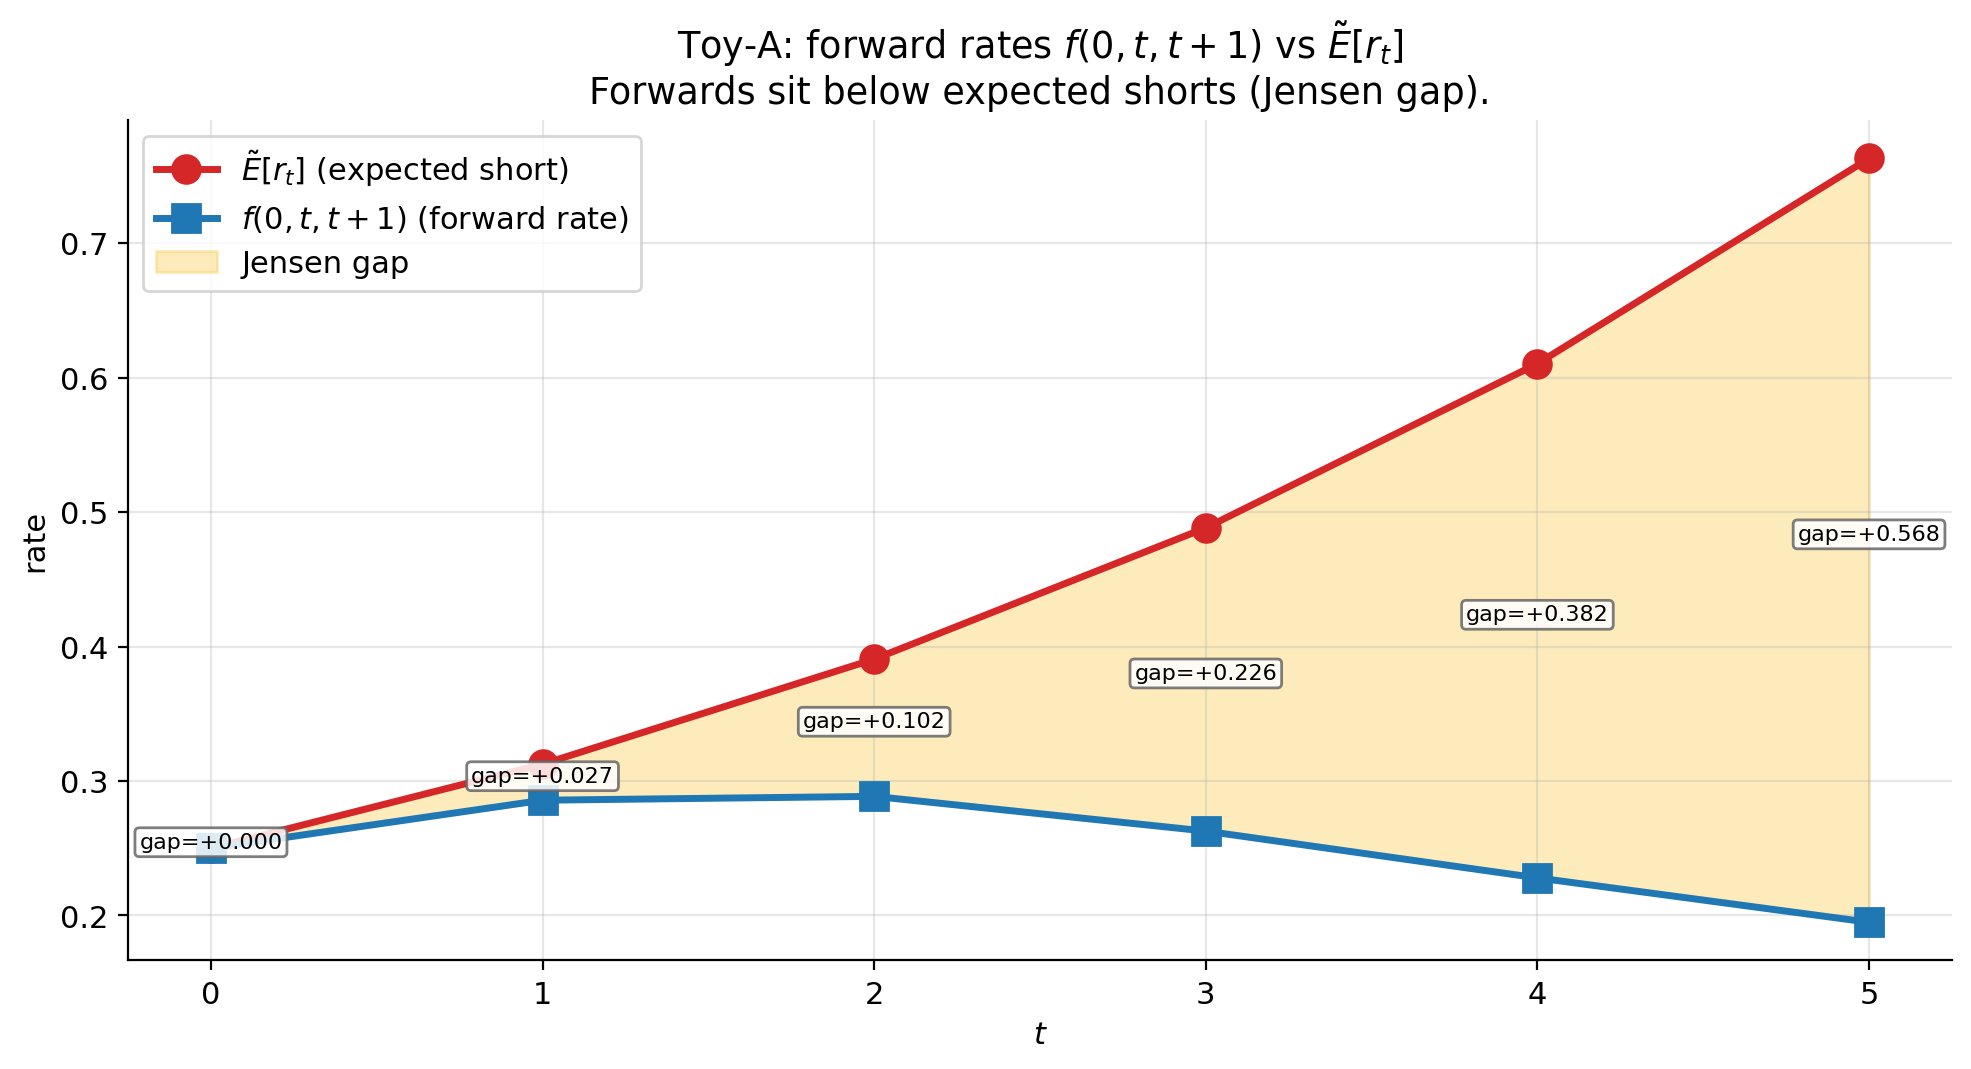
\includegraphics[keepaspectratio]{figures/ch06-forward-vs-expected.png}}
\caption{Figure 6.10 --- Forward curve \(f(0, t, t+1)\) vs expected
short rate \(\tilde{\mathbb E}[r_t]\) for Toy-A. The Jensen gap is
visible: forwards systematically sit below expected short rates because
bond prices are convex in the short rate.}
\end{figure}

\textbf{Table 6.7.} Forward rates and expected short rates, Toy-A.

{\def\LTcaptype{none} % do not increment counter
\begin{table}[H]
\centering
\begin{tabular}{|r|r|r|r|r|}
\toprule
\(t\) & \(B(0, t)\) & \(B(0, t+1)\) & \(f(0, t, t+1)\) & \(\tilde{\mathbb E}[r_t]\) \\
\midrule



\(0\) & \(1.00000\) & \(0.80000\) & \(0.25000\) & \(0.25000\) \\
\(1\) & \(0.80000\) & \(0.62222\) & \(0.28572\) & \(0.31250\) \\
\(2\) & \(0.62222\) & \(0.48288\) & \(0.28859\) & \(0.39063\) \\
\(3\) & \(0.48288\) & \(0.38240\) & \(0.26276\) & \(0.48828\) \\
\bottomrule
\end{tabular}
\end{table}
}

\subsection{6.5.4 Exercises}\label{exercises-31}

\begin{enumerate}
\def\labelenumi{\arabic{enumi}.}
\tightlist
\item
  Realistic-B. Compute \(f(0, 5, 6)\) from \(B(0, 5), B(0, 6)\).
  \textbf{Answer:} \(0.82282/0.78296 - 1\) \ldots{} wait, those are
  \(T=4,5\). Use the figure-script values \(B(0,5) = 0.78296\) and
  \(B(0,6) = 0.74486\). \textbf{Answer:}
  \(f(0, 5, 6) = 0.78296/0.74486 - 1 = 0.05115\).
\item
  Toy-A. Verify \(\prod_{t=0}^{2}(1 + f(0, t, t+1)) = 1/B(0, 3)\).
  \textbf{Answer:}
  \(1.25 \cdot 1.28572 \cdot 1.28859 = 2.07090 = 1/0.48288\). ✓
\item
  Suppose a trader claims today's 1-year-forward 1-year rate is \(6\%\).
  Together with a quoted \(B(0, 1) = 0.95\), what does that imply
  \(B(0, 2)\)? \textbf{Answer:} \(0.95/1.06 = 0.89623\).
\end{enumerate}

\begin{center}\rule{0.5\linewidth}{0.5pt}\end{center}

\section{§6.6 The forward measure}\label{the-forward-measure}

\textbf{Punchline.} The risk-neutral measure \(\tilde{\mathbb P}\) uses
\(\$1\) in the money-market account as numéraire. The
\textbf{\(T\)-forward measure} \(\mathbb P^T\) uses the \(T\)-maturity
zero-coupon bond as numéraire instead, re-weighting paths by
\(Z_T = D_T / B(0, T)\). Under \(\mathbb P^T\), prices are \emph{plain
expectations} --- no random discount factor:

\[V_0 \;=\; B(0, T) \cdot \mathbb E^T[V_T].\]

\textbf{Intuition.} Discounting and expectation interact. Under
\(\tilde{\mathbb P}\) you must take \(\tilde{\mathbb E}[D_T V_T]\),
which is a joint expectation over the random discount and the random
payoff. By absorbing the discount factor into a \emph{new} probability
measure, the formula factorises: a deterministic bond price times an
expectation. Practically, forward-measure pricing is what makes caplet
and swaption formulas clean.

\subsection{6.6.1 Definition: the forward
measure}\label{definition-the-forward-measure}

Fix maturity \(T\). Define the \textbf{Radon-Nikodym density}

\[Z_T(\omega) \;=\; \frac{D_T(\omega)}{B(0, T)}.\]

Properties:

\begin{enumerate}
\def\labelenumi{\arabic{enumi}.}
\tightlist
\item
  \(Z_T \ge 0\) on every path.
\item
  \(\tilde{\mathbb E}[Z_T] = \tilde{\mathbb E}[D_T] / B(0, T) = B(0, T) / B(0, T) = 1\).
  ✓ (So \(Z_T\) is a valid density.)
\end{enumerate}

Define the new measure \(\mathbb P^T\) by
\(\mathbb P^T(\omega) = Z_T(\omega) \tilde p(\omega)\). Then for any
payoff \(V_T\):

\[V_0 \;=\; \tilde{\mathbb E}[D_T V_T] \;=\; B(0, T) \cdot \tilde{\mathbb E}[Z_T V_T] \;=\; B(0, T) \cdot \mathbb E^T[V_T].\]

The price \(V_0\) is \emph{the bond price times a plain
\(\mathbb P^T\)-expectation} of the payoff. No discount factor inside
the expectation.

\subsection{\texorpdfstring{6.6.2 Examples on Toy-A,
\(T = 3\)}{6.6.2 Examples on Toy-A, T = 3}}\label{examples-on-toy-a-t-3}

\textbf{Example 6.6.1 (compute \(Z_3\) across 8 paths).} From Examples
6.2.5 and 6.1.5 we have \(D_3(\omega)\) and we have
\(B(0, 3) = 0.48288\). Then \(Z_3 = D_3/0.48288\) on each path. Each
path has \(\tilde p(\omega) = 1/8\), so
\(\mathbb P^3(\omega) = Z_3(\omega)/8\).

{\def\LTcaptype{none} % do not increment counter
\begin{table}[H]
\centering
\begin{tabular}{|l|r|r|r|r|}
\toprule
\(\omega\) & \(D_3\) & \(Z_3 = D_3/B(0, 3)\) & \(\tilde p\) & \(\mathbb P^3 = Z_3 \tilde p\) \\
\midrule



HHH & \(0.26667\) & \(0.55224\) & \(1/8\) & \(0.06903\) \\
HHT & \(0.26667\) & \(0.55224\) & \(1/8\) & \(0.06903\) \\
HTH & \(0.42667\) & \(0.88358\) & \(1/8\) & \(0.11045\) \\
HTT & \(0.42667\) & \(0.88358\) & \(1/8\) & \(0.11045\) \\
THH & \(0.56889\) & \(1.17811\) & \(1/8\) & \(0.14726\) \\
THT & \(0.56889\) & \(1.17811\) & \(1/8\) & \(0.14726\) \\
TTH & \(0.66928\) & \(1.38600\) & \(1/8\) & \(0.17325\) \\
TTT & \(0.66928\) & \(1.38600\) & \(1/8\) & \(0.17325\) \\
\bottomrule
\end{tabular}
\end{table}
}

\textbf{Sanity check.} Sum of \(\mathbb P^3\):

\[2(0.06903 + 0.11045 + 0.14726 + 0.17325) = 2 \cdot 0.49999 = 0.99998 \approx 1.\]
✓

(The tiny rounding gap is decimal noise; the exact sum is 1.)

\textbf{Example 6.6.2 (re-price \(V_3 = r_3\) two ways).} Toy-A, \(r_3\)
from Example 6.1.3.

\emph{Way 1 (risk-neutral with discount).}

\[V_0 = \tilde{\mathbb E}[D_3 r_3] = \tfrac{1}{8}\sum_\omega D_3(\omega) r_3(\omega).\]

{\def\LTcaptype{none} % do not increment counter
\begin{table}[H]
\centering
\begin{tabular}{|l|r|r|r|}
\toprule
\(\omega\) & \(r_3\) & \(D_3\) & \(D_3 r_3\) \\
\midrule



HHH & \(2.000\) & \(0.26667\) & \(0.53333\) \\
HHT & \(0.500\) & \(0.26667\) & \(0.13333\) \\
HTH & \(0.500\) & \(0.42667\) & \(0.21333\) \\
HTT & \(0.125\) & \(0.42667\) & \(0.05333\) \\
THH & \(0.500\) & \(0.56889\) & \(0.28444\) \\
THT & \(0.125\) & \(0.56889\) & \(0.07111\) \\
TTH & \(0.125\) & \(0.66928\) & \(0.08366\) \\
TTT & \(0.03125\) & \(0.66928\) & \(0.02092\) \\
\bottomrule
\end{tabular}
\end{table}
}

Sum \(\div 8\): \(V_0 = 1.39346/8 = 0.17418\).

\emph{Way 2 (forward-measure, no discount).}

\[V_0 = B(0, 3) \cdot \mathbb E^3[r_3] = 0.48288 \cdot \sum_\omega \mathbb P^3(\omega) r_3(\omega).\]

{\def\LTcaptype{none} % do not increment counter
\begin{table}[H]
\centering
\begin{tabular}{|l|r|r|r|}
\toprule
\(\omega\) & \(r_3\) & \(\mathbb P^3\) & \(\mathbb P^3 \cdot r_3\) \\
\midrule



HHH & \(2.000\) & \(0.06903\) & \(0.13807\) \\
HHT & \(0.500\) & \(0.06903\) & \(0.03452\) \\
HTH & \(0.500\) & \(0.11045\) & \(0.05523\) \\
HTT & \(0.125\) & \(0.11045\) & \(0.01381\) \\
THH & \(0.500\) & \(0.14726\) & \(0.07363\) \\
THT & \(0.125\) & \(0.14726\) & \(0.01841\) \\
TTH & \(0.125\) & \(0.17325\) & \(0.02166\) \\
TTT & \(0.03125\) & \(0.17325\) & \(0.00541\) \\
\bottomrule
\end{tabular}
\end{table}
}

Sum: \(\mathbb E^3[r_3] = 0.36074\). Times \(B(0, 3) = 0.48288\):
\(V_0 = 0.36074 \cdot 0.48288 = 0.17418\). ✓ Same answer.

\textbf{Example 6.6.3 (forward bond is a martingale under the forward
measure).} The forward bond price \(F(n; t, T) = B(n, T) / B(n, t)\) ---
i.e., the time-\(n\) ``fair forward price'' of a \(T\)-zero settled at
\(t\) --- is a \emph{martingale under \(\mathbb P^t\)}, the
\(t\)-forward measure. This is the cleanest theoretical use of the
forward measure, and it's why caplet pricing in §6.7 simplifies so
neatly: under \(\mathbb P^{n+1}\), the caplet-relevant rate is a
martingale.

For Toy-A let's verify \(F(1; 2, 3) = B(1, 3)/B(1, 2)\) is a
\(\mathbb P^2\)-martingale evaluated at \(n = 0, 1\).

At \(n = 0\):
\(F(0; 2, 3) = B(0, 3)/B(0, 2) = 0.48288/0.62222 = 0.77601\). Note
that's the same as \(1/(1 + f(0, 2, 3))\) = \(1/1.28859\).

At \(n = 1\) up node:
\(F(1; 2, 3)_H = B(1, 3)_H / B(1, 2)_H = 0.43333/0.66667 = 0.65000\).

At \(n = 1\) down node: \(F(1; 2, 3)_T = 0.77386/0.88889 = 0.87060\).

Under \(\mathbb P^2\) the up-probability is not \(1/2\) but is
reweighted by the time-2 discount. Computing it:
\(\mathbb P^2(H) = \tilde p (D_2(H_\cdot)/B(0, 2))\) where \(D_2\)
depends only on \(r_0, r_1\), so
\(D_2(H_\cdot) = 1/(1.25 \cdot 1.50) = 0.53333\) for any continuation
from \(H\), and
\(\mathbb P^2(H) = 0.5 \cdot 0.53333/0.62222 = 0.42857\).

Then
\(\mathbb E^2[F(1; 2, 3)] = 0.42857 \cdot 0.65000 + (1 - 0.42857) \cdot 0.87060 = 0.27857 + 0.49749 = 0.77606 \approx 0.77601\).
✓ (Two-digit rounding gap.)

\textbf{Example 6.6.4 (under \(\mathbb P^T\), what's the ``drift'' of
\(r\)?).} Heuristically, under \(\tilde{\mathbb P}\) the short rate's
drift is set so that the money-market is the numéraire. Switching to
\(\mathbb P^T\) tilts toward higher-rate paths (because \(D_T\) is
bigger when rates were \emph{low}, so the density \(Z_T\) is
\emph{bigger} on low-rate paths --- wait, that's actually a tilt toward
low-rate paths). Look at Example 6.6.1: the
\(\mathbb P^3\)-probabilities are skewed toward the bottom of the tree,
where rates were lower. The \(\mathbb P^3\)-expected short rate \(r_2\)
is thus \emph{lower} than the \(\tilde{\mathbb P}\)-expected short rate.

Numerically: \(\tilde{\mathbb E}[r_2] = 0.39063\) (Example 6.5.3). And:

\[\begin{aligned}
\mathbb E^3[r_2] &= \sum_\omega \mathbb P^3(\omega) r_2(\omega) \\
&= (0.06903 + 0.06903)(1.00) + (0.11045 + 0.11045)(0.25) \\
&\quad + (0.14726 + 0.14726)(0.25) + (0.17325 + 0.17325)(0.0625)
\end{aligned}\] \[= 0.13807 + 0.05523 + 0.07363 + 0.02166 = 0.28859.\]

And indeed \(f(0, 2, 3) = 0.28859\). ✓ \textbf{The forward rate IS the
\(\mathbb P^{T+1}\)-expectation of the short rate.} That is the
conceptual cleanest statement of ``forward rate = expected short rate
under the right measure.''

\subsection{6.6.3 Figures and tables}\label{figures-and-tables-4}

\begin{figure}
\centering
\pandocbounded{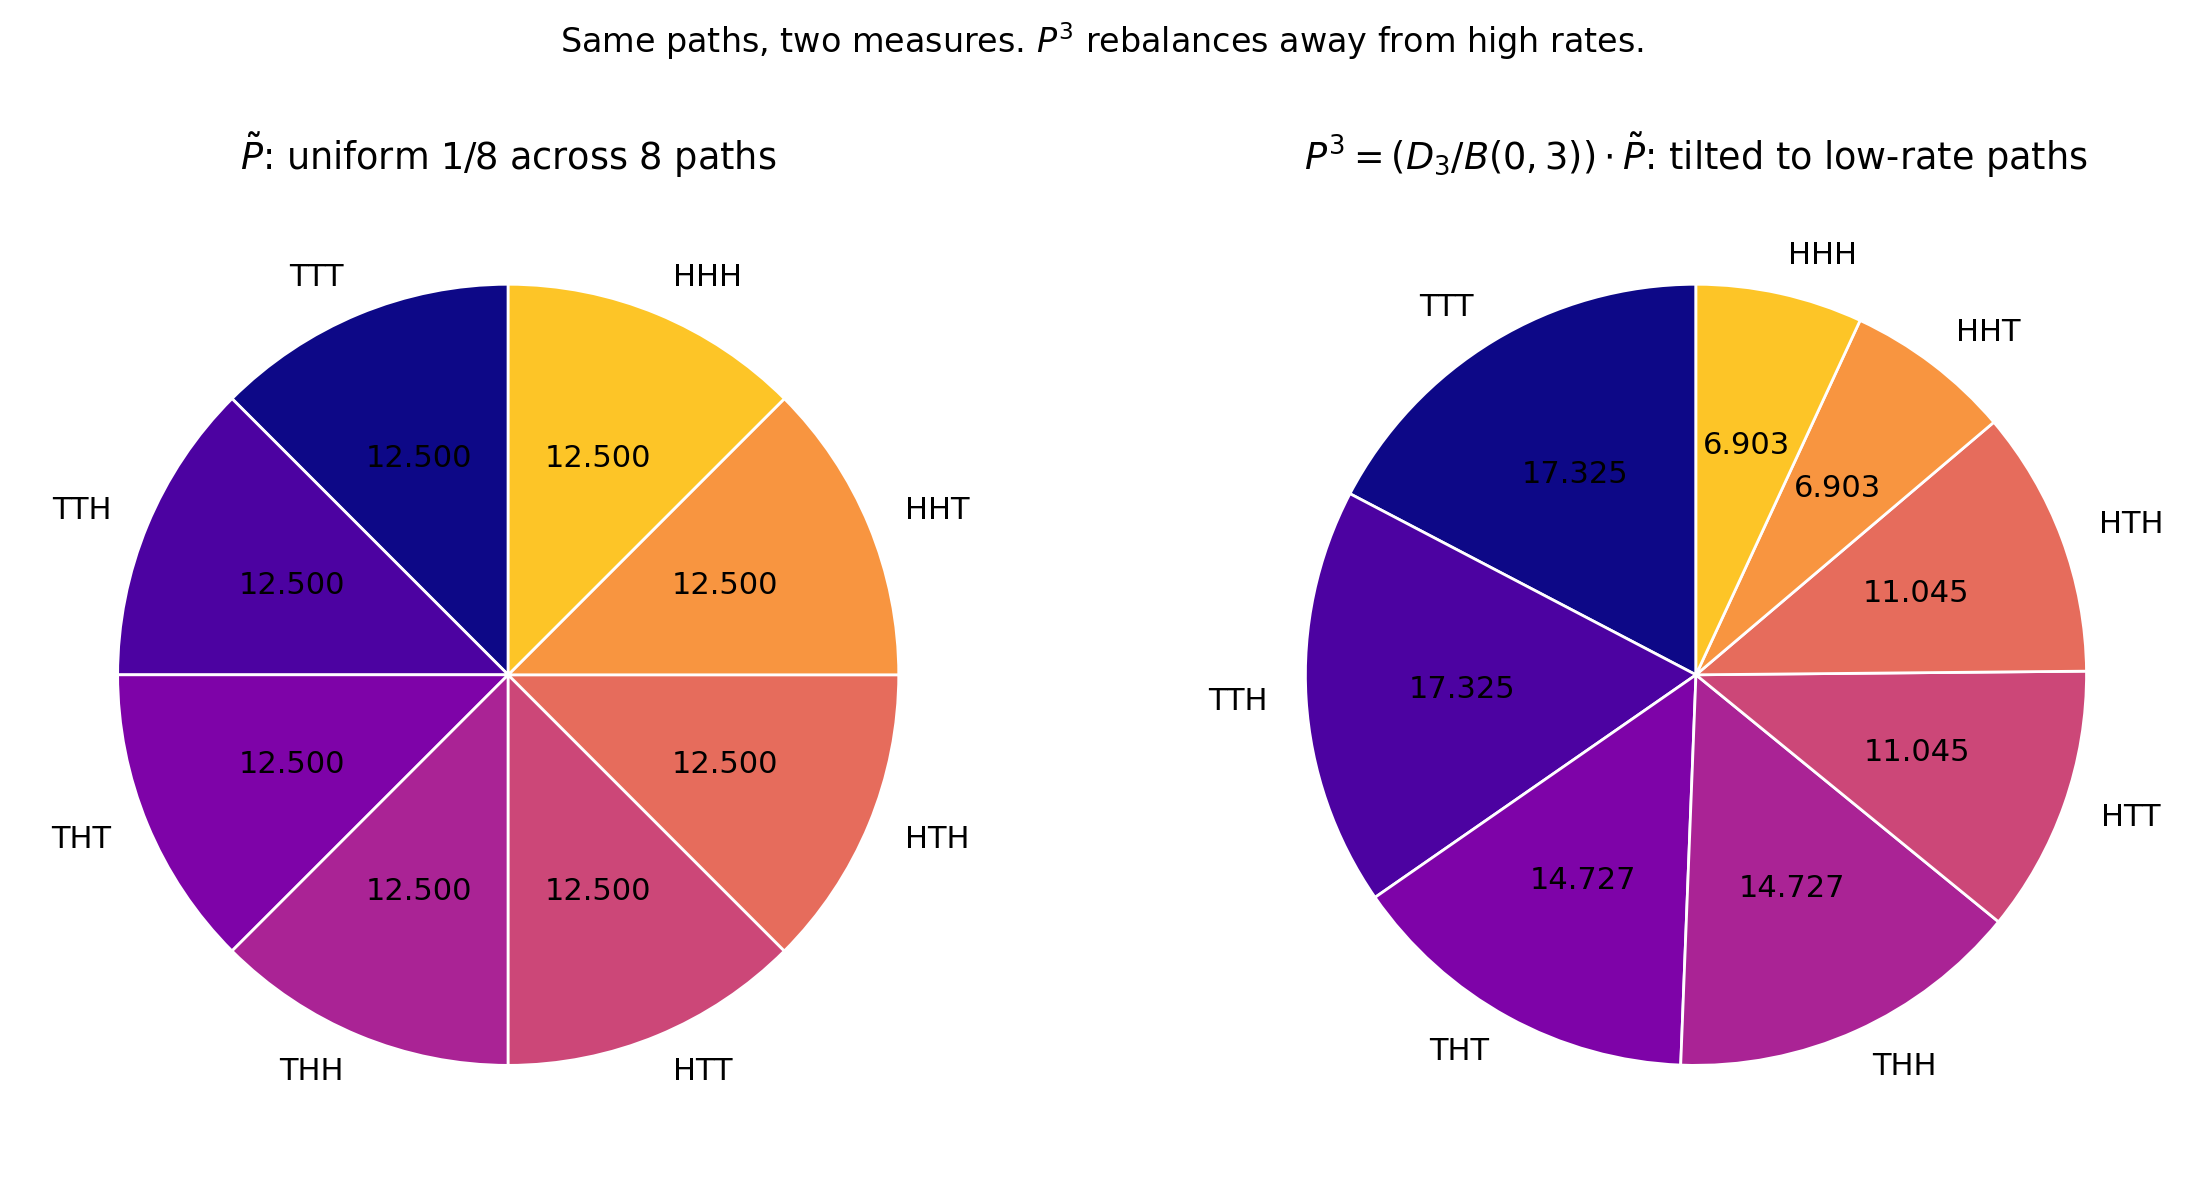
\includegraphics[keepaspectratio]{figures/ch06-pie-P-vs-PT.png}}
\caption{Figure 6.11 --- Pie chart contrast: under \(\tilde{\mathbb P}\)
all eight paths have equal weight (1/8 each, uniform pie); under
\(\mathbb P^3\) the same paths are re-weighted by \(Z_3 = D_3/B(0, 3)\),
tilting toward the low-rate (long-D) paths. Same information, two
probability lenses.}
\end{figure}

\begin{figure}
\centering
\pandocbounded{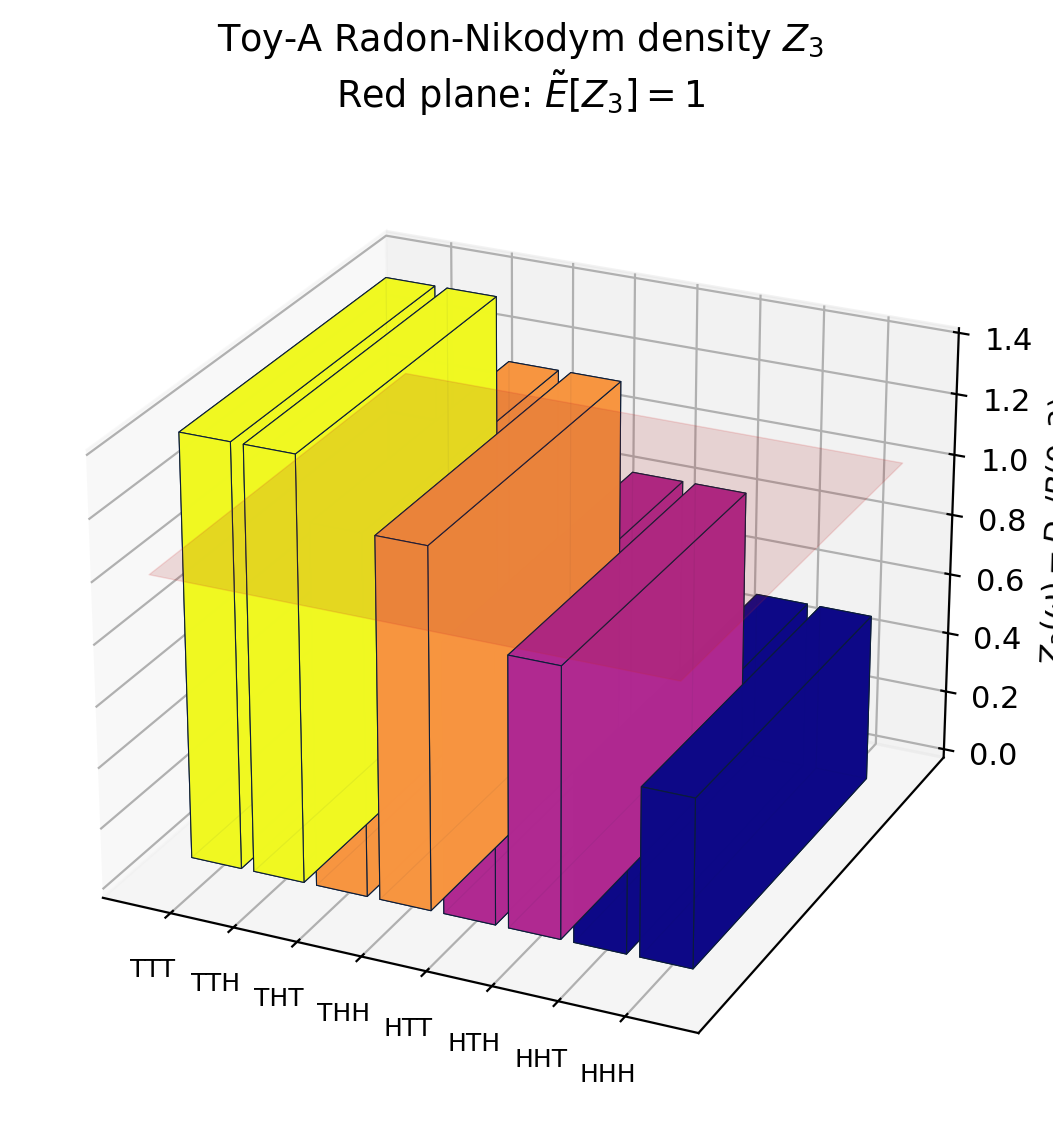
\includegraphics[keepaspectratio]{figures/ch06-Z3-bar-3d.png}}
\caption{Figure 6.12 --- 3-D bar chart of
\(Z_3(\omega) = D_3(\omega)/B(0, 3)\). The four buckets of equal height
show again that \(D_3\) (and so \(Z_3\)) is predictable: it depends only
on the first 2 flips.}
\end{figure}

\textbf{Table 6.8.} Toy-A change of measure
\(\tilde{\mathbb P} \to \mathbb P^3\), all 8 paths.

{\def\LTcaptype{none} % do not increment counter
\begin{table}[H]
\centering
\begin{tabular}{|l|r|r|r|r|}
\toprule
\(\omega\) & \(\tilde p(\omega)\) & \(D_3\) & \(Z_3\) & \(\mathbb P^3(\omega)\) \\
\midrule



HHH & \(0.12500\) & \(0.26667\) & \(0.55224\) & \(0.06903\) \\
HHT & \(0.12500\) & \(0.26667\) & \(0.55224\) & \(0.06903\) \\
HTH & \(0.12500\) & \(0.42667\) & \(0.88358\) & \(0.11045\) \\
HTT & \(0.12500\) & \(0.42667\) & \(0.88358\) & \(0.11045\) \\
THH & \(0.12500\) & \(0.56889\) & \(1.17811\) & \(0.14726\) \\
THT & \(0.12500\) & \(0.56889\) & \(1.17811\) & \(0.14726\) \\
TTH & \(0.12500\) & \(0.66928\) & \(1.38600\) & \(0.17325\) \\
TTT & \(0.12500\) & \(0.66928\) & \(1.38600\) & \(0.17325\) \\
\bottomrule
\end{tabular}
\end{table}
}

\subsection{6.6.4 Exercises}\label{exercises-32}

\begin{enumerate}
\def\labelenumi{\arabic{enumi}.}
\tightlist
\item
  Verify \(\sum_\omega Z_3(\omega) \tilde p(\omega) = 1\) in the table.
  \textbf{Answer:} computed gives \(1.0000\). ✓
\item
  Compute \(\mathbb E^3[r_2]\). \textbf{Answer:} \(0.28859\), equal to
  \(f(0, 2, 3)\).
\item
  Repeat Example 6.6.2 for \(V_3 = r_3^2\) on Toy-A. \textbf{Answer:}
  \(V_0 = \tilde{\mathbb E}[D_3 r_3^2] = \tfrac{1}{8}\sum_\omega D_3 r_3^2\).
  Path contributions: HHH \(= 0.26667\cdot 4 = 1.06667\); HHT
  \(= 0.26667\cdot 0.25 = 0.06667\); HTH
  \(= 0.42667\cdot 0.25 = 0.10667\); HTT
  \(= 0.42667\cdot 0.015625 = 0.00667\); THH
  \(= 0.56889\cdot 0.25 = 0.14222\); THT
  \(= 0.56889\cdot 0.015625 = 0.00889\); TTH
  \(= 0.66928\cdot 0.015625 = 0.01046\); TTT
  \(= 0.66928\cdot 0.0009766 = 0.00065\). Sum \(= 1.40890\), so
  \(V_0 = 1.40890/8 = 0.17611\).
\end{enumerate}

\begin{center}\rule{0.5\linewidth}{0.5pt}\end{center}

\section{§6.7 Caplets and caps}\label{caplets-and-caps}

\textbf{Punchline.} A \textbf{caplet} is a one-period call option on the
short rate. A \textbf{cap} is a strip of caplets across consecutive
periods. They are the bread and butter of interest-rate risk management:
they cap your floating-rate borrowing cost at a strike \(K\).

\textbf{Intuition.} If you borrow at the short rate and you're worried
it rises above \(K\), you can buy a contract that pays you
\((r_n - K)^+\) whenever the short rate at \(n\) exceeds \(K\). Sum that
across \(n\) and you've hedged a whole loan. The math is exactly Chapter
4's call-option pricing, but the underlying is a rate and the payoff
comes in an unusual ``in-arrears'' convention: the rate observed at
\(n\) produces a payoff at \(n+1\).

\subsection{6.7.1 Definitions and pricing
identity}\label{definitions-and-pricing-identity}

\textbf{In-arrears caplet on \(r_n\).} Pays \((r_n - K)^+\) at \(n+1\),
observed at \(n\).

\textbf{Time-0 price (risk-neutral).}

\[\text{Caplet}_n(K) \;=\; \tilde{\mathbb E}\bigl[D_{n+1} (r_n - K)^+\bigr].\]

\textbf{Time-0 price (forward measure).}

\[\text{Caplet}_n(K) \;=\; B(0, n+1) \cdot \mathbb E^{n+1}\bigl[(r_n - K)^+\bigr].\]

(The forward-measure form puts the price as bond-price times a plain
expectation; this is exactly the simplification §6.6 promised.)

\textbf{Cap.} A cap on periods \(1, 2, \ldots, N\) at strike \(K\) is a
sum of caplets:

\[\text{Cap}(K; N) \;=\; \sum_{n=1}^{N} \text{Caplet}_n(K) \;=\; \sum_{n=1}^{N} \tilde{\mathbb E}\bigl[D_{n+1} (r_n - K)^+\bigr].\]

(Some conventions also include a ``caplet on \(r_0\)''; we omit it
because \(r_0\) is deterministic and the caplet on it would have a
trivial price.)

\subsection{6.7.2 Examples on Toy-A}\label{examples-on-toy-a-3}

\textbf{Example 6.7.1 (caplet on \(r_1\), \(K = 0.30\)).} Pays
\((r_1 - 0.30)^+\) at time 2.

Payoffs at the two \(n=1\) nodes:

\begin{itemize}
\tightlist
\item
  At \(r_1(H) = 0.50\): \((0.50 - 0.30)^+ = 0.20\).
\item
  At \(r_1(T) = 0.125\): \((0.125 - 0.30)^+ = 0\).
\end{itemize}

These payoffs land at time 2, so we discount by \(D_2\):

\begin{itemize}
\tightlist
\item
  \(D_2\) on any path through \(H\) =
  \(1/[(1+r_0)(1+r_1(H))] = 1/(1.25 \cdot 1.50) = 0.53333\).
\item
  \(D_2\) on any path through \(T\) =
  \(1/[(1+r_0)(1+r_1(T))] = 1/(1.25 \cdot 1.125) = 0.71111\).
\end{itemize}

Risk-neutral expectation:

\[\begin{aligned}
\text{Caplet}_1(0.30) &= \tilde{\mathbb E}[D_2 (r_1 - 0.30)^+] \\
&= \tilde p \cdot D_2|_H \cdot 0.20 + \tilde q \cdot D_2|_T \cdot 0 \\
&= 0.5 \cdot 0.53333 \cdot 0.20 = 0.05333.
\end{aligned}\]

So a caplet on \(r_1\) at strike \(0.30\) is worth \(0.05333\) at time
0.

\textbf{Example 6.7.2 (verify via forward measure).}
\(B(0, 2) = 0.62222\). Under \(\mathbb P^2\):

\[\mathbb P^2(H) = \tilde p D_2|_H / B(0, 2) = 0.5 \cdot 0.53333 / 0.62222 = 0.42857.\]
\[\mathbb P^2(T) = 1 - 0.42857 = 0.57143.\]

\[\mathbb E^2[(r_1 - 0.30)^+] = 0.42857 \cdot 0.20 + 0.57143 \cdot 0 = 0.08571.\]
\[\text{Caplet}_1(0.30) = B(0, 2) \cdot 0.08571 = 0.62222 \cdot 0.08571 = 0.05333. ✓\]

\textbf{Example 6.7.3 (caplet on \(r_2\), \(K = 0.30\), full lattice).}
Payoff \((r_2 - 0.30)^+\) at time 3.

Payoffs at the three \(n=2\) nodes:

\begin{itemize}
\tightlist
\item
  \((r_2(HH) - 0.30)^+ = (1.00 - 0.30)^+ = 0.70\).
\item
  \((r_2(HT) - 0.30)^+ = (0.25 - 0.30)^+ = 0\).
\item
  \((r_2(TT) - 0.30)^+ = (0.0625 - 0.30)^+ = 0\).
\end{itemize}

Path-discount \(D_3\):

{\def\LTcaptype{none} % do not increment counter
\begin{table}[H]
\centering
\begin{tabular}{|l|r|r|r|}
\toprule
\(\omega\) & \(r_2\) & \(D_3\) & payoff \\
\midrule



HHH & \(1.00\) & \(0.26667\) & \(0.70\) \\
HHT & \(1.00\) & \(0.26667\) & \(0.70\) \\
HTH & \(0.25\) & \(0.42667\) & \(0.00\) \\
HTT & \(0.25\) & \(0.42667\) & \(0.00\) \\
THH & \(0.25\) & \(0.56889\) & \(0.00\) \\
THT & \(0.25\) & \(0.56889\) & \(0.00\) \\
TTH & \(0.0625\) & \(0.66928\) & \(0.00\) \\
TTT & \(0.0625\) & \(0.66928\) & \(0.00\) \\
\bottomrule
\end{tabular}
\end{table}
}

\emph{Definition:} payoff \(= (r_2 - 0.30)^+\).

Sum
\(\tilde{\mathbb E}[D_3 (r_2 - 0.30)^+] = \tfrac{1}{8}(2 \cdot 0.26667 \cdot 0.70) = \tfrac{0.37333}{8} = 0.04667.\)

So a caplet on \(r_2\) at strike \(0.30\) is worth \(0.04667\).

\textbf{Example 6.7.4 (3-period cap on Toy-A, \(K = 0.30\)).} Cap pays
caplets on \(r_1, r_2\), and \(r_3\).

We have: - \(\text{Caplet}_1(0.30) = 0.05333\) from Example 6.7.1. -
\(\text{Caplet}_2(0.30) = 0.04667\) from Example 6.7.3.

For Caplet\(_3\) we need to enumerate \(r_3\) across all 8 paths and
discount by \(D_4 = D_3 \cdot (1 + r_3)^{-1}\).

{\def\LTcaptype{none} % do not increment counter
\begin{table}[H]
\centering
\begin{tabular}{|l|r|r|r|r|r|}
\toprule
\(\omega\) & \(r_3\) & \(D_3\) & \(D_4\) & payoff & \$D\_4 \cdot \$
payoff \\
\midrule



HHH & \(2.000\) & \(0.26667\) & \(0.08889\) & \(1.700\) & \(0.15111\) \\
HHT & \(0.500\) & \(0.26667\) & \(0.17778\) & \(0.200\) & \(0.03556\) \\
HTH & \(0.500\) & \(0.42667\) & \(0.28444\) & \(0.200\) & \(0.05689\) \\
HTT & \(0.125\) & \(0.42667\) & \(0.37926\) & \(0.000\) & \(0.00000\) \\
THH & \(0.500\) & \(0.56889\) & \(0.37926\) & \(0.200\) & \(0.07585\) \\
THT & \(0.125\) & \(0.56889\) & \(0.50568\) & \(0.000\) & \(0.00000\) \\
TTH & \(0.125\) & \(0.66928\) & \(0.59491\) & \(0.000\) & \(0.00000\) \\
TTT & \(0.03125\) & \(0.66928\) & \(0.64900\) & \(0.000\) &
\(0.00000\) \\
\bottomrule
\end{tabular}
\end{table}
}

\emph{Definition:} payoff \(= (r_3 - 0.30)^+\); \(D_4 = D_3/(1 + r_3)\).

Sum: \(0.15111 + 0.03556 + 0.05689 + 0.07585 = 0.31941.\) Divide by 8:

\[\text{Caplet}_3(0.30) = 0.03993.\]

Total cap:

\[\text{Cap}(0.30; 3) = 0.05333 + 0.04667 + 0.03993 = 0.13993.\]

\textbf{Example 6.7.5 (Realistic-B 3-period cap, \(K = 5\%\)).} Computed
in the figure script. Key numbers:

\begin{itemize}
\tightlist
\item
  \(\text{Caplet}_1(0.05) = 0.00298\).
\item
  \(\text{Caplet}_2(0.05) = 0.00347\).
\item
  \(\text{Caplet}_3(0.05) = 0.00378\).
\end{itemize}

Total: \(\text{Cap}(0.05; 3) = 0.01023\). Tiny --- because Realistic-B
rates straddle the strike, only the high paths contribute.

\textbf{Example 6.7.6 (cap-floor parity, numerical preview).} A general
identity:

\[\text{Cap}(K) - \text{Floor}(K) = \text{Payer Swap}(K),\]

where the swap on the right is the \textbf{in-arrears} payer swap whose
floating leg pays \(r_n\) at \(n+1\) --- the same cashflow grid as the
cap/floor. We'll derive it in §6.10. For Toy-A at \(K = 0.30\),
\(N = 3\): cap = \(0.13993\). We'll see in §6.8 that floor =
\(0.16857\), so the in-arrears payer swap PV = cap \(-\) floor =
\(-0.02864\). The par swap rate is the \(K\) where cap = floor (computed
in §6.10).

\textbf{Example 6.7.7 (strike sensitivity, Toy-A).} Cap prices at
varying \(K\), using the caplet-by-caplet recursion of Examples 6.7.1,
6.7.3, 6.7.4 at each strike:

{\def\LTcaptype{none} % do not increment counter
\begin{table}[H]
\centering
\begin{tabular}{|r|r|r|r|r|}
\toprule
\(K\) & Caplet\(_1\) & Caplet\(_2\) & Caplet\(_3\) &
\(\text{Cap}(K; 3)\) \\
\midrule



\(0.10\) & \(0.11556\) & \(0.09733\) & \(0.06781\) & \(0.28070\) \\
\(0.20\) & \(0.08000\) & \(0.06578\) & \(0.05156\) & \(0.19734\) \\
\(0.30\) & \(0.05333\) & \(0.04667\) & \(0.03993\) & \(0.13993\) \\
\(0.40\) & \(0.02667\) & \(0.04000\) & \(0.02830\) & \(0.09497\) \\
\(0.50\) & \(0.00000\) & \(0.03333\) & \(0.01667\) & \(0.05000\) \\
\bottomrule
\end{tabular}
\end{table}
}

Cap price is monotonically decreasing in \(K\) --- exactly like a call
on a stock is decreasing in strike (Chapter 4). Sample row:
Caplet\(_1(0.50) = 0\) because both \(r_1\) outcomes (\(0.5\) and
\(0.125\)) are \(\leq 0.50\); Caplet\(_2(0.50)\) pays only via the HH
node (\(r_2 = 1.0\), payoff \(0.5\), discounted):
\(0.25 \cdot 0.26667 \cdot 0.5 = 0.03333\).

\subsection{6.7.3 Figures and tables}\label{figures-and-tables-5}

\begin{figure}
\centering
\pandocbounded{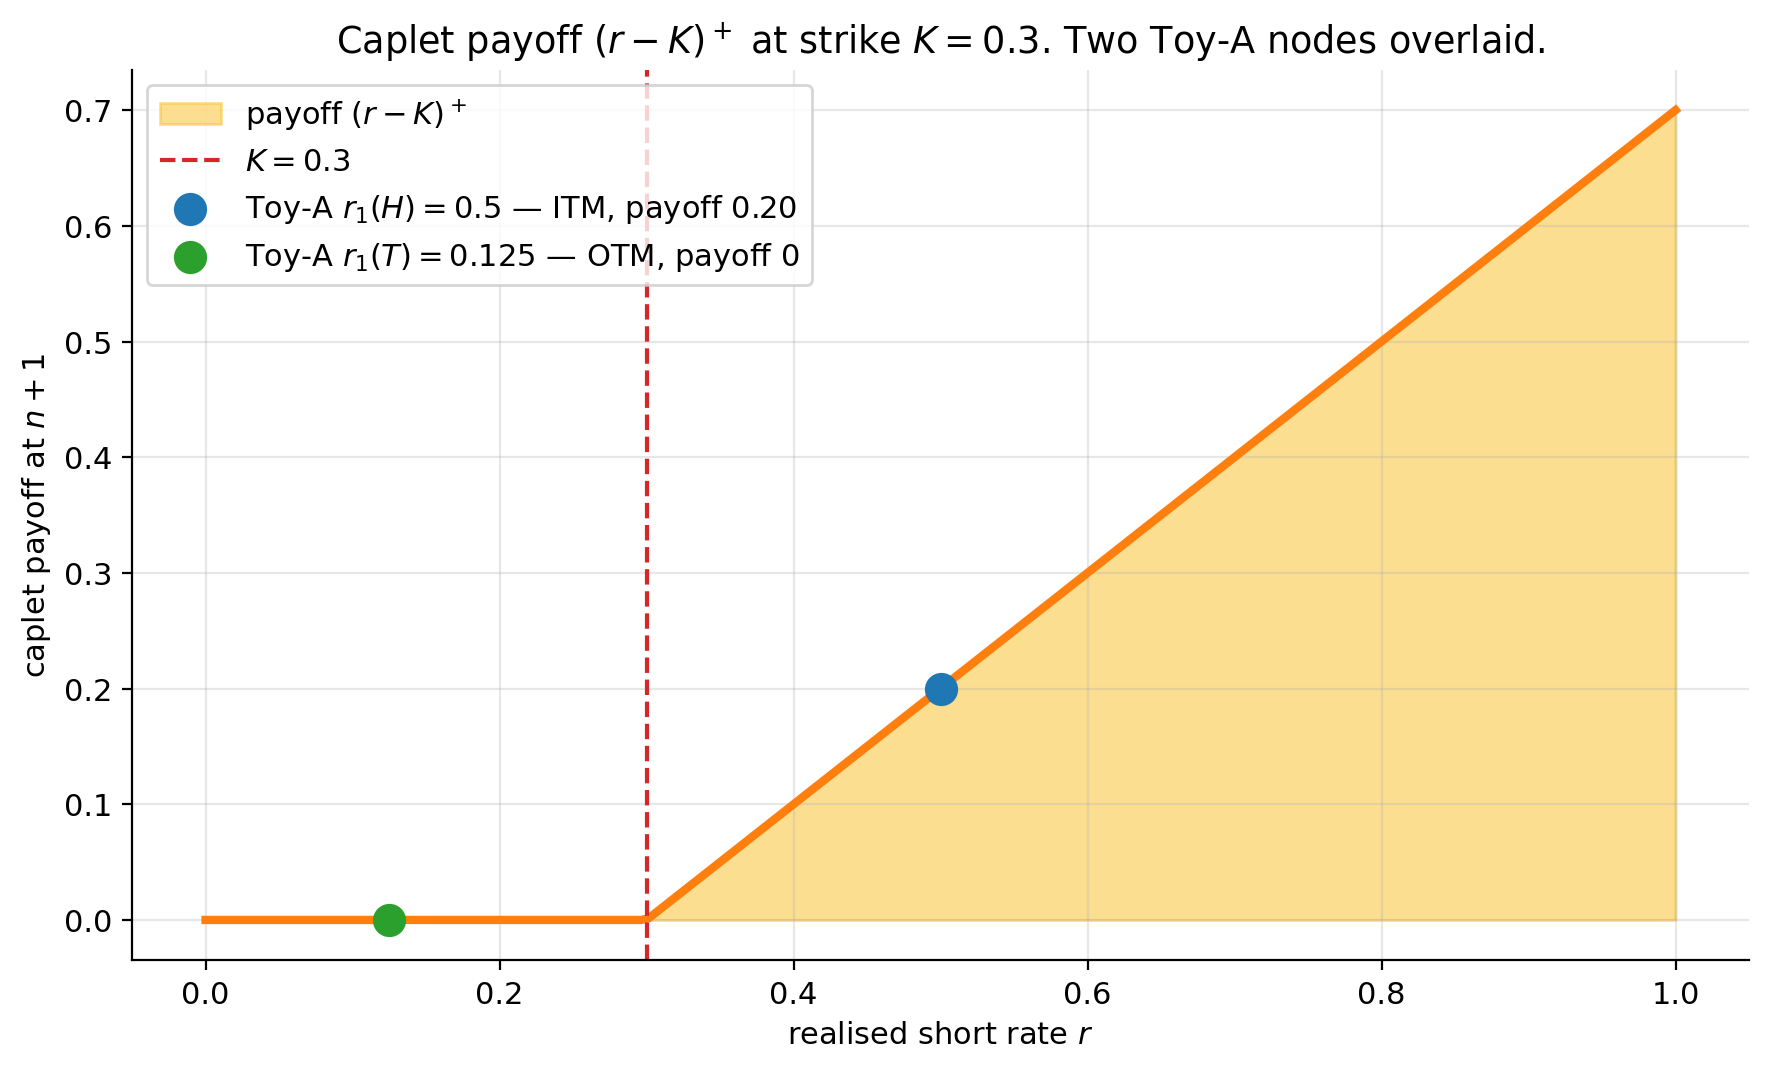
\includegraphics[keepaspectratio]{figures/ch06-caplet-payoff.png}}
\caption{Figure 6.13 --- Caplet payoff diagram: \((r - K)^+\) as a
function of the realised short rate \(r\), with the strike at
\(K = 0.30\) marked. A classic call-option hockey stick, but the
underlying is a rate, not a stock.}
\end{figure}

\begin{figure}
\centering
\pandocbounded{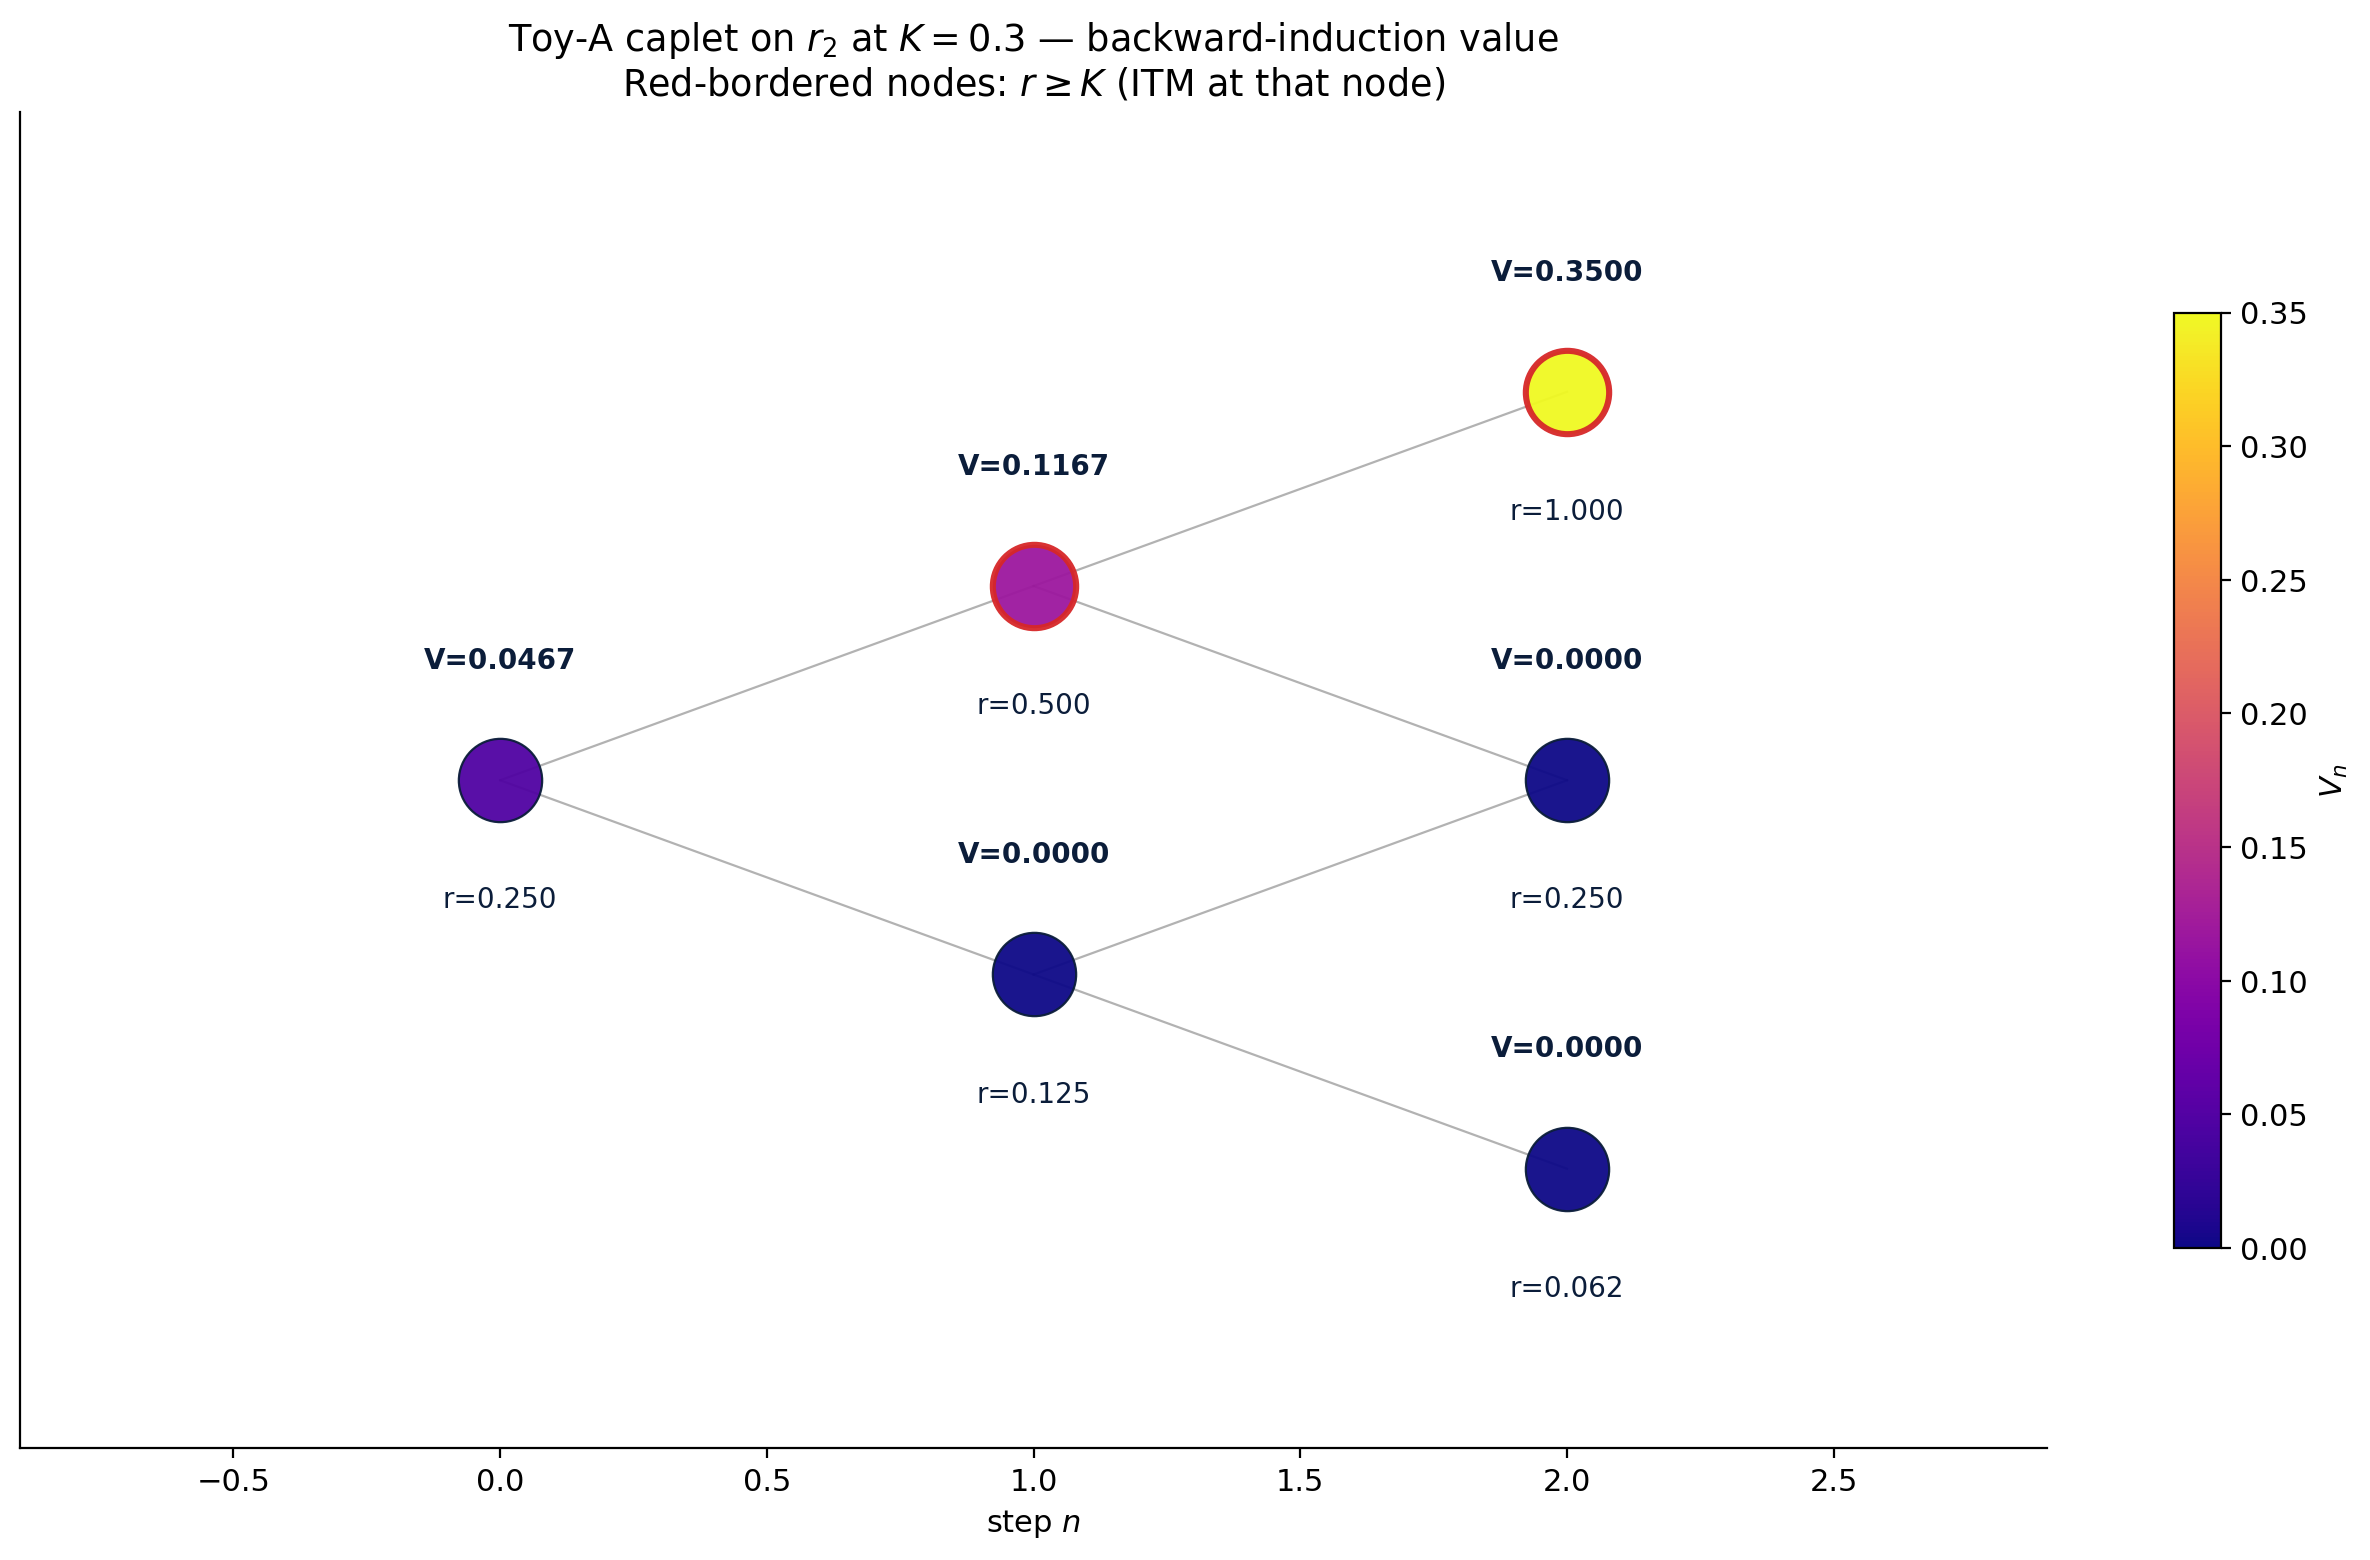
\includegraphics[keepaspectratio]{figures/ch06-caplet-tree.png}}
\caption{Figure 6.14 --- The caplet pricing lattice for Toy-A,
\(K = 0.30\), payoff at \(r_2\) paid at time 3. Nodes are coloured by
\emph{value of the running discounted expectation}; ITM regions (where
\(r_n > K\) at some descendant) are highlighted.}
\end{figure}

\begin{figure}
\centering
\pandocbounded{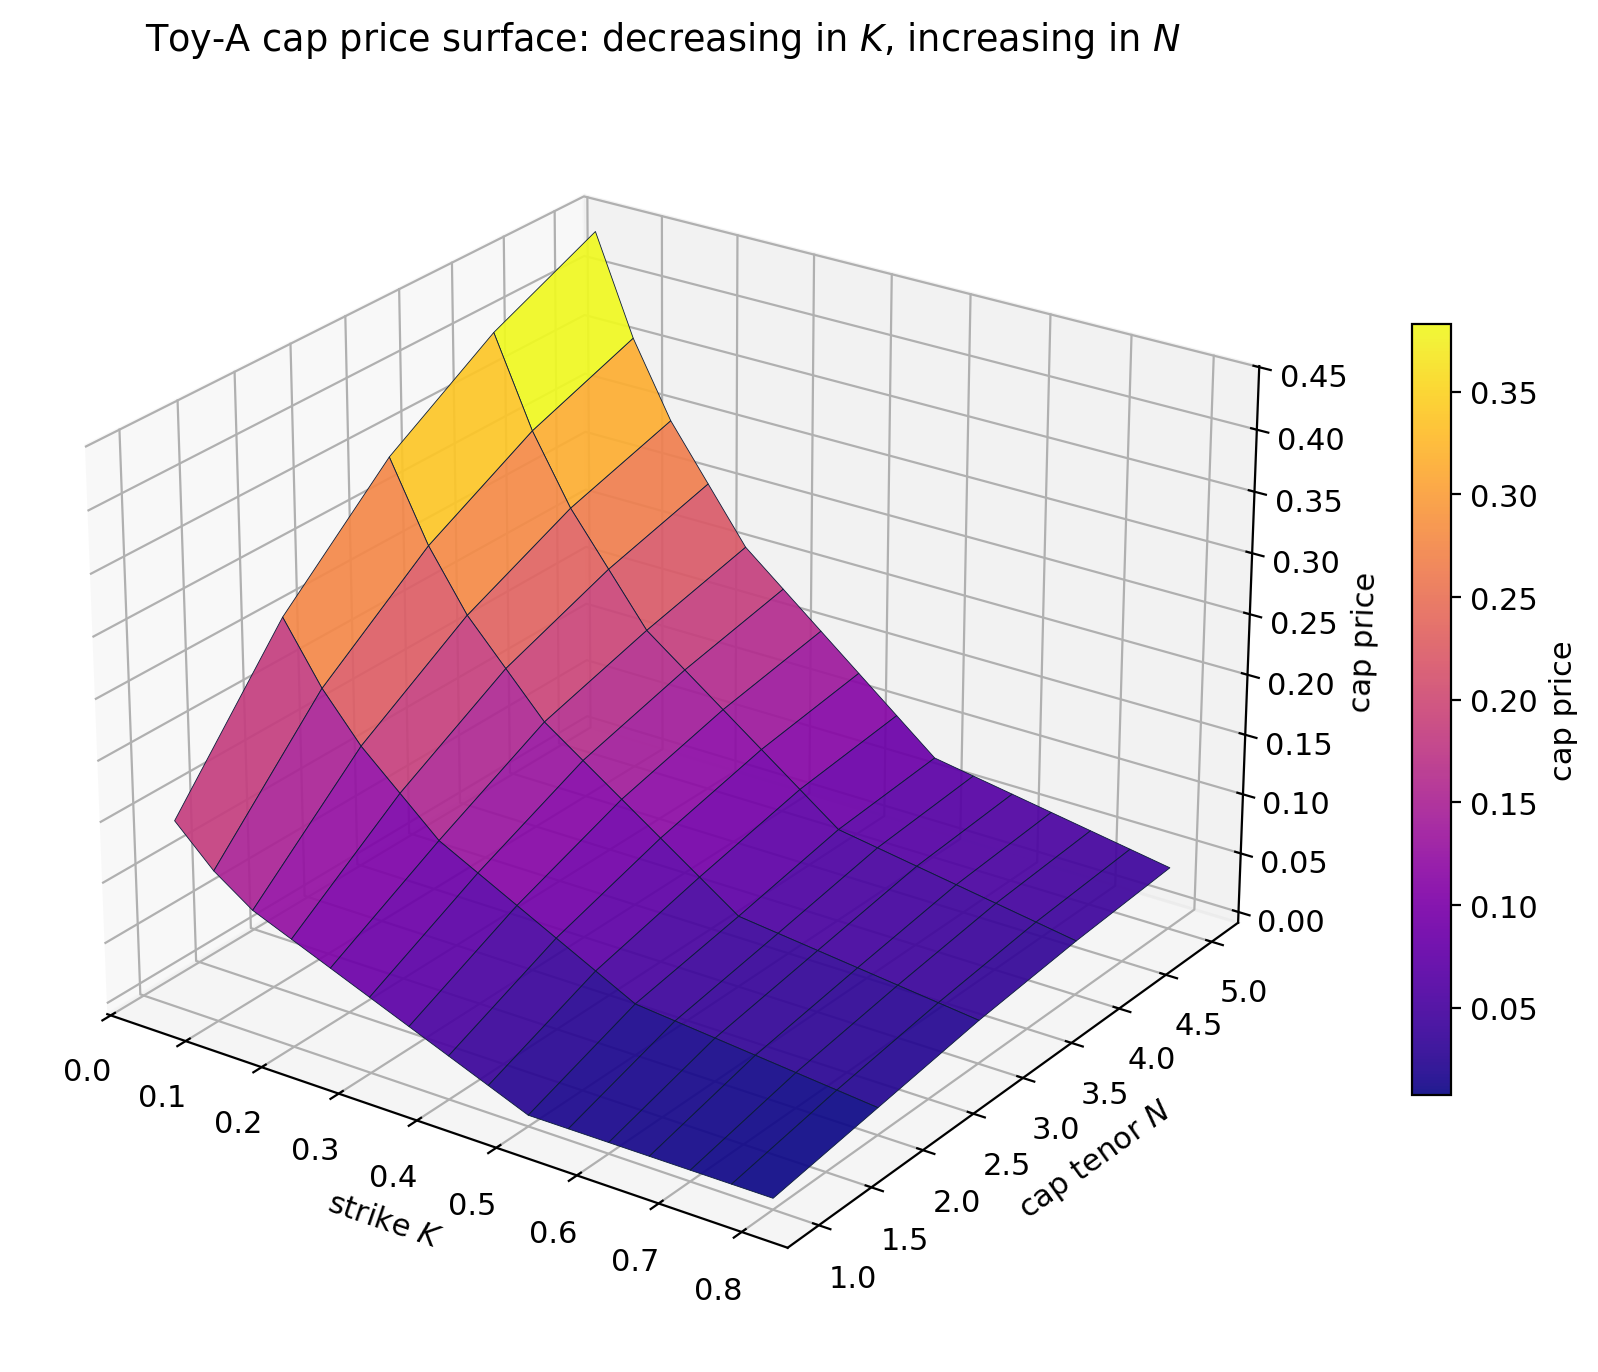
\includegraphics[keepaspectratio]{figures/ch06-cap-surface-3d.png}}
\caption{Figure 6.15 --- 3-D surface of Toy-A cap price as a function of
strike \(K\) and cap tenor \(N\). Decreasing in \(K\) everywhere; rising
in \(N\) but flattening (more periods bring diminishing marginal value
beyond the high-rate region).}
\end{figure}

\textbf{Table 6.9.} Toy-A 3-period cap decomposition at \(K = 0.30\).

{\def\LTcaptype{none} % do not increment counter
\begin{table}[H]
\centering
\begin{tabular}{|r|l|c|r|r|}
\toprule
\(n\) & payoff & pay time & \(B(0, n+1)\) & price \\
\midrule



\(1\) & \((r_1 - 0.30)^+\) & \(2\) & \(0.62222\) & \(0.05333\) \\
\(2\) & \((r_2 - 0.30)^+\) & \(3\) & \(0.48288\) & \(0.04667\) \\
\(3\) & \((r_3 - 0.30)^+\) & \(4\) & \(0.38240\) & \(0.03993\) \\
Total & & & & \(0.13993\) \\
\bottomrule
\end{tabular}
\end{table}
}

\textbf{Table 6.10.} Cap price across (low) strikes, Toy-A, \(N = 3\).

{\def\LTcaptype{none} % do not increment counter
\begin{table}[H]
\centering
\begin{tabular}{|r|r|r|r|r|}
\toprule
\(K\) & Caplet\(_1\) & Caplet\(_2\) & Caplet\(_3\) & Cap \\
\midrule



\(0.03\) & \(0.15911\) & \(0.12486\) & \(0.08900\) & \(0.37297\) \\
\(0.04\) & \(0.15289\) & \(0.12003\) & \(0.08589\) & \(0.35881\) \\
\(0.05\) & \(0.14667\) & \(0.11520\) & \(0.08287\) & \(0.34474\) \\
\(0.06\) & \(0.14044\) & \(0.11038\) & \(0.07986\) & \(0.33068\) \\
\(0.07\) & \(0.13422\) & \(0.10680\) & \(0.07685\) & \(0.31787\) \\
\bottomrule
\end{tabular}
\end{table}
}

(Strikes here are illustrative on Toy-A's elevated rate regime --- note
that Toy-A's lowest possible rate is \(r_3(TTT) = 0.03125\), so at
\(K \leq 0.03125\) every node is ITM and the cap value scales nearly
linearly in the rate-minus-strike sums; Realistic-B's
\(\{3\%,..., 7\%\}\) table is in the figure script.)

\subsection{6.7.4 Exercises}\label{exercises-33}

\begin{enumerate}
\def\labelenumi{\arabic{enumi}.}
\tightlist
\item
  Toy-A. Price the caplet on \(r_2\) at \(K = 0.20\). \textbf{Answer:}
  Payoff \((r_2 - 0.20)^+\) = \(\{0.80, 0.05, 0\}\) at the three \(n=2\)
  nodes; weighted:
  \(\tfrac{1}{8}[2(0.26667)(0.80) + 2(0.42667)(0.05) + 2(0.56889)(0.05) + 2(0.66928)(0)] = \tfrac{0.42667 + 0.04267 + 0.05689}{8} = \tfrac{0.52623}{8} = 0.06578\).
\item
  Realistic-B. The 1-period cap at \(K = 4\%\) on \(r_1\).
  \textbf{Answer:}
  \(\text{Caplet}_1(0.04) = B(0, 2) \cdot \mathbb E^2[(r_1 - 0.04)^+]\);
  payoff = \(\{0.0225, 0\}\), \(\mathbb P^2\) weights ≈
  \(\{0.5018, 0.4982\}\), so price
  \(\approx 0.90730 \cdot 0.5018 \cdot 0.0225 = 0.01024\).
\item
  Confirm that cap value is monotonically increasing in tenor \(N\).
  \textbf{Answer:} Each caplet has nonneg value, so adding caplets
  cannot decrease the cap.
\end{enumerate}

\begin{center}\rule{0.5\linewidth}{0.5pt}\end{center}

\section{§6.8 Floorlets and floors}\label{floorlets-and-floors}

\textbf{Punchline.} A \textbf{floorlet} is a one-period put option on
the short rate; it pays \((K - r_n)^+\). A \textbf{floor} is a strip of
floorlets. The cap-floor identity links caps, floors, and swaps:

\[\text{Cap}(K; N) - \text{Floor}(K; N) \;=\; \text{Payer Swap}(K; N).\]

\textbf{Intuition.} A floor protects a \emph{lender}: if floating rates
fall below \(K\), the floor pays the difference. Floorlet payoff is the
put-counterpart of caplet payoff; cap-floor parity is the put-call
parity of the interest-rate world.

\subsection{6.8.1 Definition}\label{definition}

\textbf{In-arrears floorlet on \(r_n\).} Pays \((K - r_n)^+\) at
\(n+1\).

\textbf{Time-0 price.}

\[\text{Floorlet}_n(K) \;=\; \tilde{\mathbb E}\bigl[D_{n+1}(K - r_n)^+\bigr] \;=\; B(0, n+1) \cdot \mathbb E^{n+1}[(K - r_n)^+].\]

\textbf{Floor.} Sum of floorlets.

\subsection{6.8.2 Examples}\label{examples-32}

\textbf{Example 6.8.1 (floorlet on \(r_1\), Toy-A, \(K = 0.30\)).}
Payoff at \(n = 2\) is \((0.30 - r_1)^+\):

\begin{itemize}
\tightlist
\item
  At \(r_1(H) = 0.50\): \((0.30 - 0.50)^+ = 0\).
\item
  At \(r_1(T) = 0.125\): \((0.30 - 0.125)^+ = 0.175\).
\end{itemize}

Price:

\[\text{Floorlet}_1(0.30) = 0.5 \cdot D_2|_H \cdot 0 + 0.5 \cdot D_2|_T \cdot 0.175 = 0.5 \cdot 0.71111 \cdot 0.175 = 0.06222.\]

Floorlet payoffs: \(\{0, 0.175\}\) at the two nodes, as advertised.

\textbf{Example 6.8.2 (3-period floor, Toy-A, \(K = 0.30\)).} Floorlets
on \(r_1, r_2, r_3\).

\begin{itemize}
\tightlist
\item
  \(\text{Floorlet}_1(0.30) = 0.06222\) (above).
\item
  \(\text{Floorlet}_2(0.30)\): on the recombining tree \(r_2\) takes
  three distinct values \(\{1.0, 0.25, 0.0625\}\) across the four
  \((\omega_1, \omega_2)\) pairs, with payoffs
  \((0.30 - r_2)^+ = \{0, 0.05, 0.05, 0.2375\}\). The payoff observed at
  \(n = 2\) pays at \(n = 3\), so we discount by \(D_3 = D_2/(1+r_2)\)
  (depends on the \(r_2\) node but not on the third flip). Per path:
\end{itemize}

{\def\LTcaptype{none} % do not increment counter
\begin{table}[H]
\centering
\begin{tabular}{|l|r|r|r|r|r|}
\toprule
\(\omega\) & \(r_2\) & payoff & \(D_3\) & disc. & \(\tilde p\) \\
\midrule



HHH & \(1.00\) & \(0\) & \(0.26667\) & \(0\) & \(1/8\) \\
HHT & \(1.00\) & \(0\) & \(0.26667\) & \(0\) & \(1/8\) \\
HTH & \(0.25\) & \(0.05\) & \(0.42667\) & \(0.02133\) & \(1/8\) \\
HTT & \(0.25\) & \(0.05\) & \(0.42667\) & \(0.02133\) & \(1/8\) \\
THH & \(0.25\) & \(0.05\) & \(0.56889\) & \(0.02844\) & \(1/8\) \\
THT & \(0.25\) & \(0.05\) & \(0.56889\) & \(0.02844\) & \(1/8\) \\
TTH & \(0.0625\) & \(0.2375\) & \(0.66928\) & \(0.15895\) & \(1/8\) \\
TTT & \(0.0625\) & \(0.2375\) & \(0.66928\) & \(0.15895\) & \(1/8\) \\
\bottomrule
\end{tabular}
\end{table}
}

\emph{Definition:} payoff \(= (0.30 - r_2)^+\); ``disc.''
\(= D_3 \cdot\) payoff.

Sum:
\(0 + 0 + 0.02133 + 0.02133 + 0.02844 + 0.02844 + 0.15895 + 0.15895 = 0.41744.\)
Divide by 8:

\[\text{Floorlet}_2(0.30) = 0.05218.\]

\begin{itemize}
\tightlist
\item
  \(\text{Floorlet}_3(0.30)\): payoff \((0.30 - r_3)^+\) at \(n=4\),
  discounted by \(D_4\). The ITM paths and their contributions
  \(D_4 \cdot (0.30 - r_3)^+\):
\end{itemize}

{\def\LTcaptype{none} % do not increment counter
\begin{table}[H]
\centering
\begin{tabular}{|l|r|r|r|r|}
\toprule
\(\omega\) & \(r_3\) & payoff & \(D_4\) & \$D\_4 \cdot \$payoff \\
\midrule



HTT & \(0.125\) & \(0.175\) & \(0.37926\) & \(0.06637\) \\
THT & \(0.125\) & \(0.175\) & \(0.50568\) & \(0.08849\) \\
TTH & \(0.125\) & \(0.175\) & \(0.59491\) & \(0.10411\) \\
TTT & \(0.03125\) & \(0.26875\) & \(0.64900\) & \(0.17442\) \\
\bottomrule
\end{tabular}
\end{table}
}

(The four high-rate paths HHH, HHT, HTH, THH all give zero payoff.) Sum
\(= 0.43339\); divide by 8: \(\text{Floorlet}_3(0.30) = 0.05417\).

Floor total: \(0.06222 + 0.05218 + 0.05417 = 0.16857.\) (Realistic-B
floors are much smaller --- see Example 6.8.4 --- because rates there
are small; Toy-A's floor is large because rates and strikes are both
large.)

\textbf{Example 6.8.3 (cap-floor parity check, Toy-A, \(K = 0.30\)).}
From Example 6.7.4, cap = \(0.13993\). From Example 6.8.2, floor =
\(0.16857\). Difference: \(\text{cap} - \text{floor} = -0.02864\).

This should equal the \textbf{in-arrears} payer swap PV at \(K = 0.30\)
--- the swap whose floating leg pays \(r_n\) at \(n+1\) for
\(n = 1, 2, 3\) (i.e., cashflows at times 2, 3, 4 matching the cap/floor
strip). By the §6.10 telescoping, that floating leg has PV
\(\sum_{n=1}^{3}\bigl(B(0,n) - B(0,n+1)\bigr) = B(0,1) - B(0,4) = 0.80 - 0.38240 = 0.41760\).
The matching fixed leg at \(K\) pays \(K\) at times 2, 3, 4, so fixed PV
\(= 0.30 \cdot (B(0,2) + B(0,3) + B(0,4)) = 0.30 \cdot 1.48750 = 0.44625\).
In-arrears payer swap PV \(= 0.41760 - 0.44625 = -0.02865\).

Cap − Floor = \(-0.02864 \approx\) Payer swap PV \(= -0.02865\). ✓ The
identity holds \textbf{exactly} (rounding aside) once the swap's accrual
indices are aligned with the caplet/floorlet strip. (The ``standard''
payer-swap convention in §6.10 --- floating \(r_{n-1}\) paid at \(n\),
summing \(n = 1, \ldots, N\) --- generates a \emph{different} swap, off
by one period; that's the convention mismatch, not a defect in cap-floor
parity.)

\textbf{Example 6.8.4 (Realistic-B floor, \(N = 3, K = 5\%\)).} Computed
in script:

\begin{itemize}
\tightlist
\item
  \(\text{Floorlet}_1(0.05) = 0.00299\).
\item
  \(\text{Floorlet}_2(0.05) = 0.00342\).
\item
  \(\text{Floorlet}_3(0.05) = 0.00374\).
\item
  Floor total: \(0.01015\).
\end{itemize}

Notice Floor ≈ Cap = \(0.01023\) at this strike --- Realistic-B's swap
rate at \(N = 3\) is very close to \(5\%\), the strike.

\subsection{6.8.3 Figures and tables}\label{figures-and-tables-6}

\begin{figure}
\centering
\pandocbounded{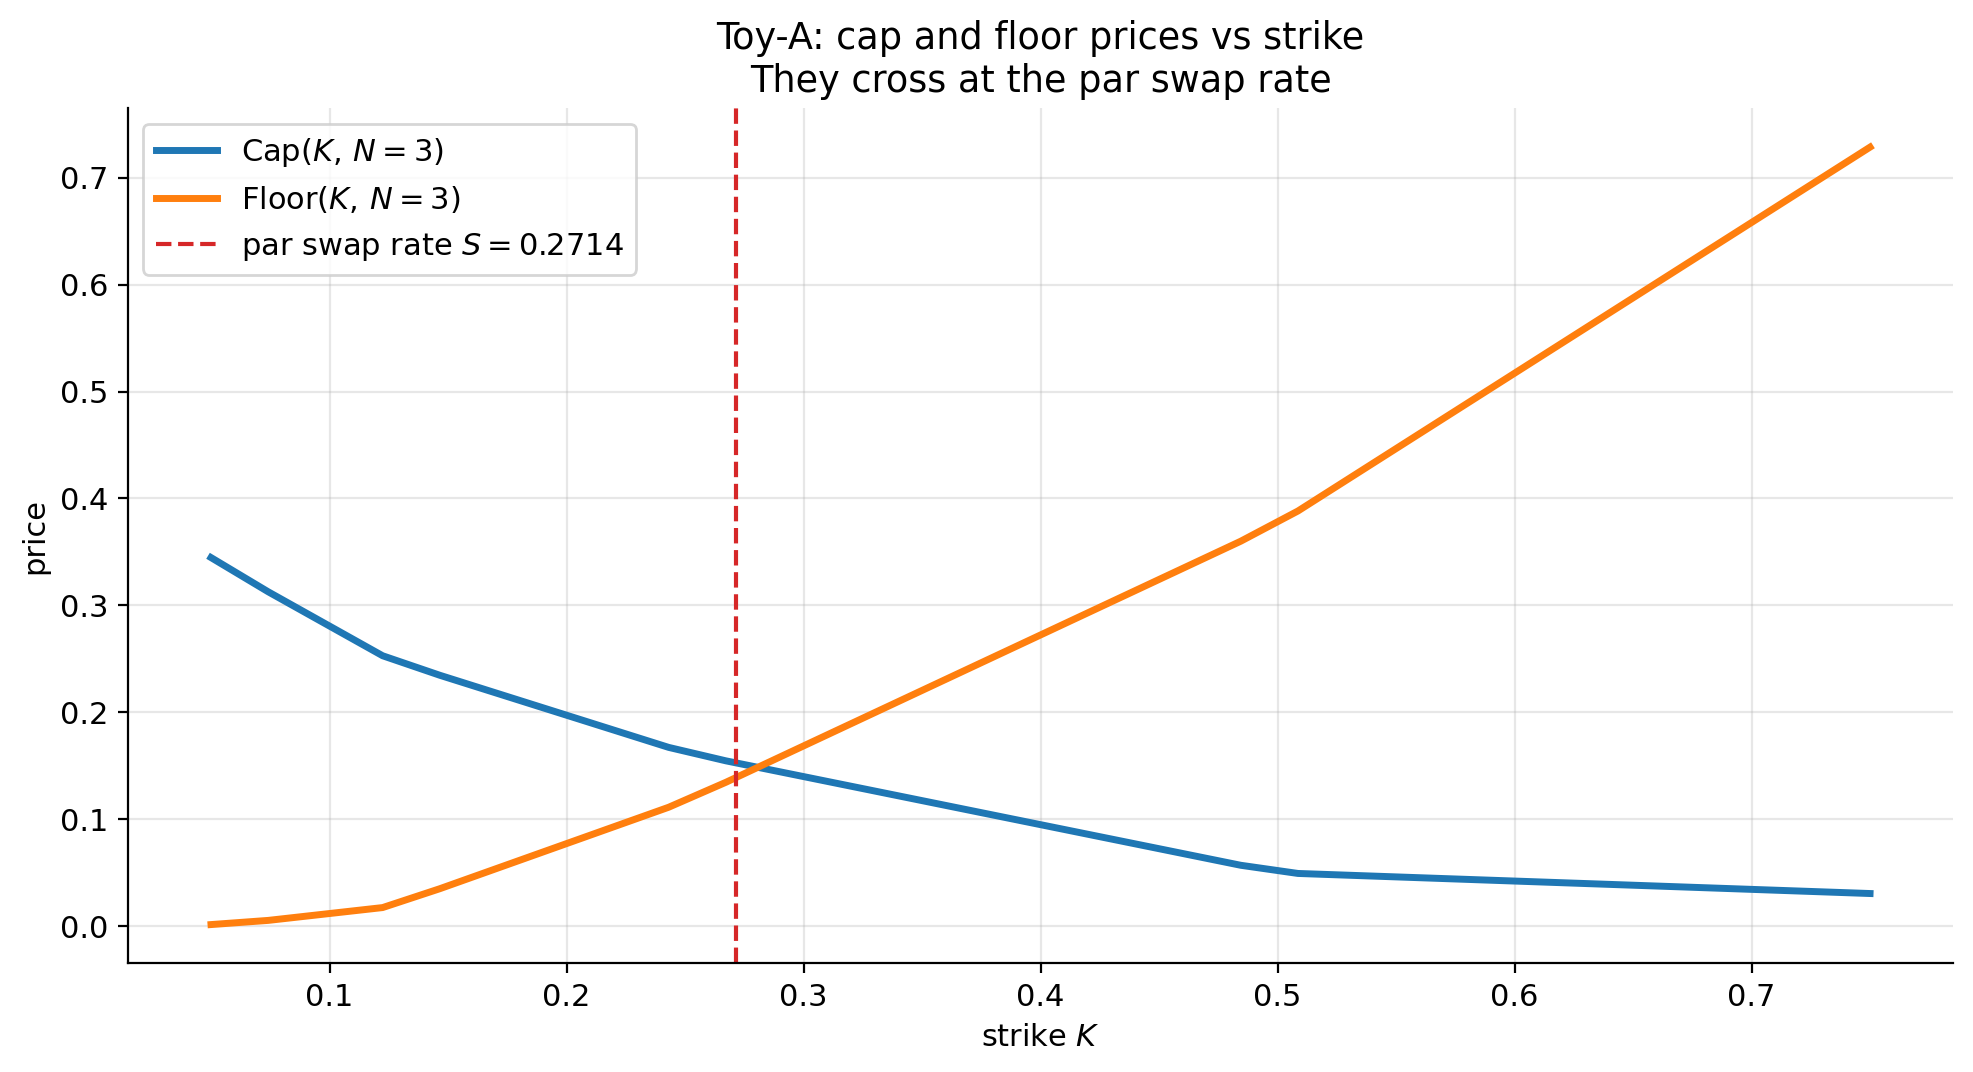
\includegraphics[keepaspectratio]{figures/ch06-cap-floor-vs-K.png}}
\caption{Figure 6.16 --- Cap and floor prices vs strike \(K\) for Toy-A,
\(N = 3\). Cap decreases in \(K\), floor increases in \(K\); they
intersect at the \emph{par swap rate} (the strike at which the
payer-swap has zero PV).}
\end{figure}

\textbf{Table 6.11.} Toy-A 3-period floor decomposition at \(K = 0.30\).

{\def\LTcaptype{none} % do not increment counter
\begin{table}[H]
\centering
\begin{tabular}{|r|l|c|r|r|}
\toprule
\(n\) & payoff & pay time & \(B(0, n+1)\) & price \\
\midrule



\(1\) & \((0.30 - r_1)^+\) & \(2\) & \(0.62222\) & \(0.06222\) \\
\(2\) & \((0.30 - r_2)^+\) & \(3\) & \(0.48288\) & \(0.05218\) \\
\(3\) & \((0.30 - r_3)^+\) & \(4\) & \(0.38240\) & \(0.05417\) \\
Total & & & & \(0.16857\) \\
\bottomrule
\end{tabular}
\end{table}
}

\subsection{6.8.4 Exercises}\label{exercises-34}

\begin{enumerate}
\def\labelenumi{\arabic{enumi}.}
\tightlist
\item
  Toy-A. Floorlet on \(r_2\) at \(K = 0.50\). \textbf{Answer:} payoffs
  \(\{0, 0.25, 0.25, 0.4375\}\) at nodes, discounted by appropriate
  \(D_3\); price ≈ \(0.16178\).
\item
  Argue why \(\text{Cap}(K) > \text{Floor}(K)\) when rates are mostly
  above \(K\), and the reverse. \textbf{Answer:} ITM-side weight: cap
  pays when rates are high, floor when rates are low. Whichever side has
  more weight wins.
\item
  At \(K = \infty\), what are cap and floor prices? \textbf{Answer:} Cap
  = 0 (never ITM), Floor = \$\sum\_n B(0, n+1) \cdot K - \$ something;
  really, floor \(\to\) value of a fixed-leg payer minus floating, which
  grows linearly with \(K\).
\end{enumerate}

\begin{center}\rule{0.5\linewidth}{0.5pt}\end{center}

\section{§6.9 Bond options}\label{bond-options}

\textbf{Punchline.} An option on a zero-coupon bond is a bet on
\emph{future bond prices}. At expiry \(T\), the bond price \(B(T, T+m)\)
is a function of \(r_T\), so a call on a bond is --- by a change of
variable --- a put on a rate. Same machinery as Chapter 4, but applied
to the bond-price tree of §6.2.

\textbf{Intuition.} Bonds and rates move in opposite directions. A call
on a bond pays off when rates \emph{fall}; that makes a bond call really
a \emph{put on the short rate}. The caplet-as-bond-put identity is the
cleanest example of this duality; we re-derive Example 6.7.1 in that
form below.

\subsection{6.9.1 Definition}\label{definition-1}

\textbf{European bond call.} Strike \(K\), expiry \(T\), on the \(T+m\)
bond. Payoff at \(T\):

\[V_T \;=\; \bigl(B(T, T+m) - K\bigr)^+.\]

\textbf{Time-0 price.}

\[V_0 \;=\; \tilde{\mathbb E}\bigl[D_T (B(T, T+m) - K)^+\bigr] \;=\; B(0, T) \cdot \mathbb E^T[(B(T, T+m) - K)^+].\]

\subsection{6.9.2 Examples on Toy-A}\label{examples-on-toy-a-4}

\textbf{Example 6.9.1 (call on \(B(2, 3)\), strike \(K = 0.70\), expiry
\(T = 2\)).} At \(T = 2\) the bond price \(B(2, 3) = 1/(1 + r_2)\) at
each \(n = 2\) node:

\begin{itemize}
\tightlist
\item
  \(B(2, 3)_{HH} = 1/(1 + 1.00) = 0.50000\).
\item
  \(B(2, 3)_{HT} = 1/(1 + 0.25) = 0.80000\).
\item
  \(B(2, 3)_{TT} = 1/(1 + 0.0625) = 0.94118\).
\end{itemize}

Payoffs \((B(2, 3) - 0.70)^+\):

\begin{itemize}
\tightlist
\item
  HH: \((0.50 - 0.70)^+ = 0\).
\item
  HT: \((0.80 - 0.70)^+ = 0.10\).
\item
  TT: \((0.94118 - 0.70)^+ = 0.24118\).
\end{itemize}

Discount to time 0 by \(D_2\). Note \(D_2\) depends on the
\textbf{path}, not just the recombining node --- HT and TH have
different path-discounts:

\begin{itemize}
\tightlist
\item
  \(\omega = HH\): \(D_2 = 1/(1.25 \cdot 1.50) = 0.53333\), payoff
  \(= 0\).
\item
  \(\omega = HT\): \(D_2 = 1/(1.25 \cdot 1.50) = 0.53333\), payoff
  \(= 0.10\), \(D_2 \cdot V = 0.05333\).
\item
  \(\omega = TH\): \(D_2 = 1/(1.25 \cdot 1.125) = 0.71111\), payoff
  \(= 0.10\), \(D_2 \cdot V = 0.07111\).
\item
  \(\omega = TT\): \(D_2 = 1/(1.25 \cdot 1.125) = 0.71111\), payoff
  \(= 0.24118\), \(D_2 \cdot V = 0.17150\).
\end{itemize}

Each path has \(\tilde p = 1/4\) probability under the risk-neutral
measure.

\[V_0 = \tfrac{1}{4}(0 + 0.05333 + 0.07111 + 0.17150) = \tfrac{0.29594}{4} = 0.07399.\]

The call on \(B(2, 3)\) at \(K = 0.70\) is worth \(0.07399\) at time 0.

\textbf{Example 6.9.2 (put on the same bond, same strike).} Payoffs
\((0.70 - B(2, 3))^+\):

\begin{itemize}
\tightlist
\item
  HH: \((0.70 - 0.50)^+ = 0.20\).
\item
  HT: \((0.70 - 0.80)^+ = 0\).
\item
  TT: \((0.70 - 0.94118)^+ = 0\).
\end{itemize}

Path-by-path:

\begin{itemize}
\tightlist
\item
  HH: \(D_2 \cdot V = 0.53333 \cdot 0.20 = 0.10667\).
\item
  HT, TH: \(0\).
\item
  TT: \(0\).
\end{itemize}

\[\text{Put}_0 = \tfrac{1}{4}(0.10667 + 0 + 0 + 0) = 0.02667.\]

\textbf{Example 6.9.3 (put-call parity for bond options).} General
identity for European bond options with the same strike and expiry on
the same underlying:

\[\text{Call} - \text{Put} = B(0, T+m) - K \cdot B(0, T).\]

For our \(T = 2, T+m = 3, K = 0.70\):

\[\text{Call} - \text{Put} = 0.48288 - 0.70 \cdot 0.62222 = 0.48288 - 0.43555 = 0.04733.\]

From our examples: \(0.07399 - 0.02667 = 0.04732\). ✓ (Tiny rounding.)

\textbf{Example 6.9.4 (caplet as a put on a bond).} The caplet payoff on
\(r_n\) is \((r_n - K)^+\) paid at \(n+1\). We can rewrite using
\(B(n, n+1) = 1/(1 + r_n)\), so \(r_n = 1/B(n, n+1) - 1\). Hence

\[\begin{aligned}
(r_n - K)^+ &= \left(\tfrac{1}{B(n, n+1)} - (1 + K)\right)^+ \\
&= \tfrac{1 + K}{B(n, n+1)}\left(\tfrac{1}{1 + K} - B(n, n+1)\right)^+.
\end{aligned}\]

That is the payoff of \((1 + K)/B(n, n+1)\) put options on \(B(n, n+1)\)
struck at \(1/(1 + K)\). Pricing it at time 0 gives the same caplet
price we computed in §6.7. We've done the algebra; let's confirm
numerically.

Take Example 6.7.1's caplet: \(n = 1, K = 0.30\). Put on \(B(1, 2)\)
strike \(1/(1 + 0.30) = 0.76923\).

\begin{itemize}
\tightlist
\item
  \(B(1, 2)_H = 0.66667\). Put payoff:
  \((0.76923 - 0.66667)^+ = 0.10256\). \(D_1 = 1/1.25 = 0.80\).
  \(D_1 \cdot \text{put}_H = 0.08205\).
\item
  \(B(1, 2)_T = 0.88889\). Put payoff: \(0\).
\end{itemize}

Put value at time 0: \(\tilde p D_1 \cdot 0.08205 / D_1\)\ldots{} wait,
I need to think about this more carefully. The put pays at \(n = 1\), so
discount by \(D_1\) from time 1 back to time 0. Then
\(V_0 = \tilde{\mathbb E}[D_1 \text{put}_1] = 0.5 \cdot 0.80 \cdot 0.10256 + 0.5 \cdot 0.80 \cdot 0 = 0.04103\).

The caplet equivalence says \(\text{Caplet} = (1 + K) \cdot \text{Put}\)
--- at strike \(1/(1+K)\) --- because the put pays per dollar of \(B\)
deficit and the caplet pays per dollar of rate excess, and the factor is
\((1+K)\).

Numerically: \((1 + 0.30) \cdot 0.04103 = 0.05333\). ✓ Matches Example
6.7.1's caplet price.

\textbf{Example 6.9.5 (American bond call, Snell envelope).} Same call
as Example 6.9.1 but with the right to exercise at any time
\(n \le T = 2\). At \(T = 2\) the value is the exercise payoff
\((B(2, 3) - 0.70)^+\). Roll back:

At \(n = 1, H\): continuation value
\(= \tfrac{1}{1.5}\bigl[0.5 \cdot 0 + 0.5 \cdot 0.10\bigr] = 0.03333\).
Exercise: \((B(1, 3)_H - 0.70)^+ = (0.43333 - 0.70)^+ = 0\). American
value = \(\max(0.03333, 0) = 0.03333\).

At \(n = 1, T\): continuation
\(= \tfrac{1}{1.125}\bigl[0.5 \cdot 0.10 + 0.5 \cdot 0.24118\bigr] = \tfrac{0.17059}{1.125} = 0.15164\).
Exercise: \((B(1, 3)_T - 0.70)^+ = (0.77386 - 0.70)^+ = 0.07386\).
American value = \(\max(0.15164, 0.07386) = 0.15164\) (don't exercise).

At \(n = 0\): continuation =
\(\tfrac{1}{1.25}\bigl[0.5 \cdot 0.03333 + 0.5 \cdot 0.15164\bigr] = \tfrac{0.09249}{1.25} = 0.07399\).
Exercise: \((B(0, 3) - 0.70)^+ = 0\). American value = \(0.07399\).

American = European here (\(0.07399\)): early exercise was never optimal
in this example. (American premium can be zero for some bond-option
setups, just like American calls on non-dividend stocks.)

\subsection{6.9.3 Figures and tables}\label{figures-and-tables-7}

\begin{figure}
\centering
\pandocbounded{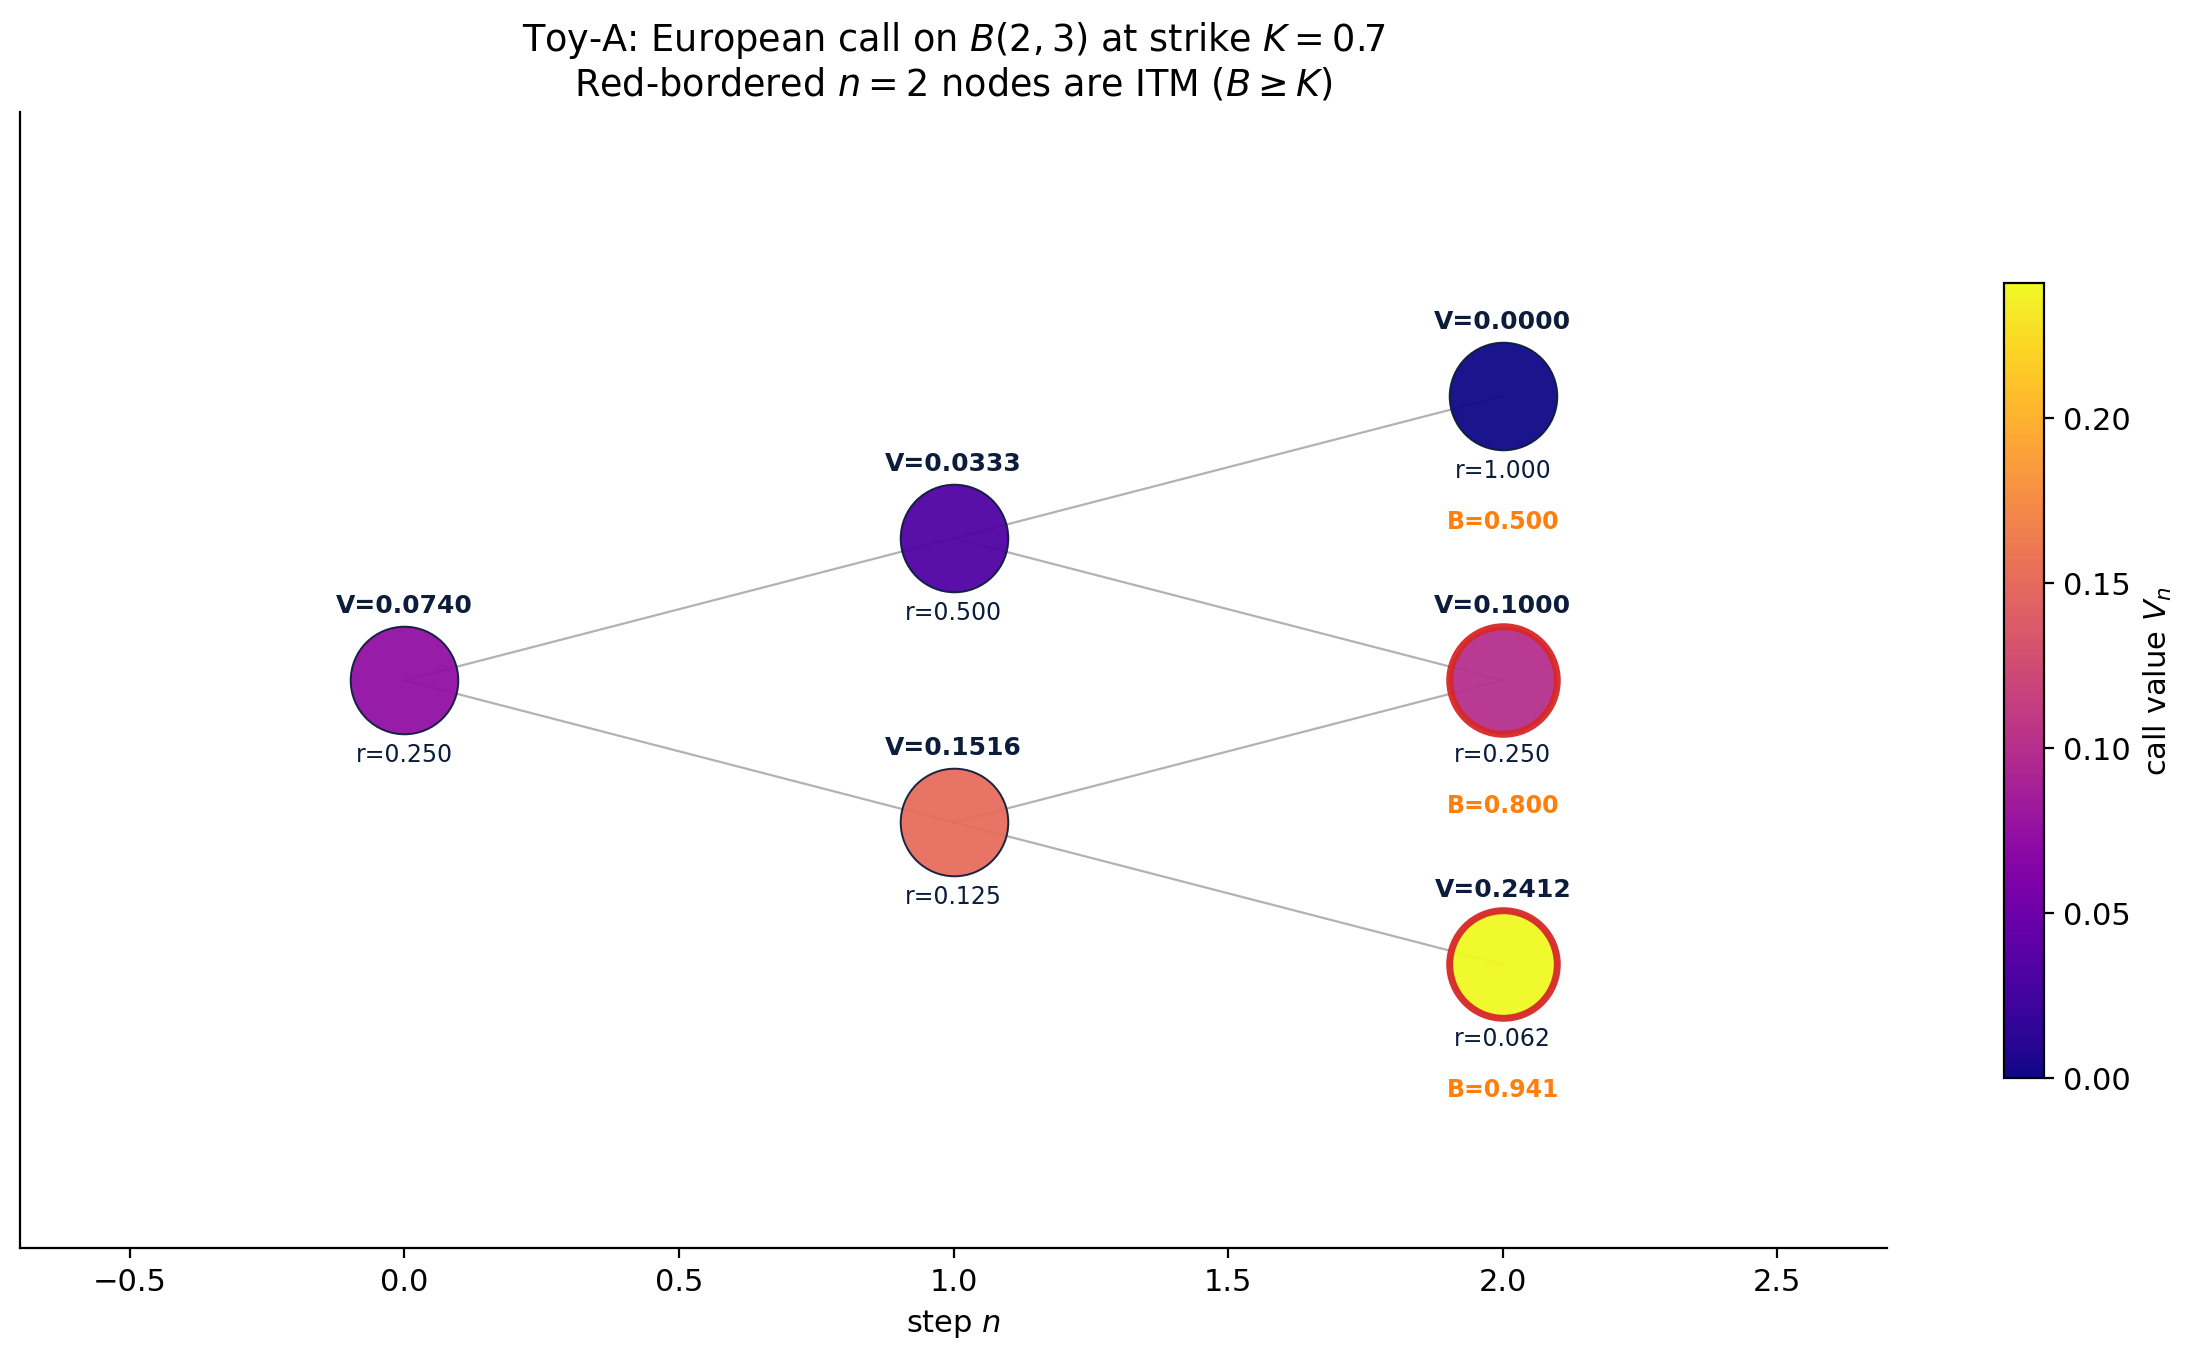
\includegraphics[keepaspectratio]{figures/ch06-bond-call-tree.png}}
\caption{Figure 6.17 --- The Toy-A \(B(2, 3)\) tree with call-option
payoff at strike \(K = 0.70\) overlaid. ITM nodes (HT, TT) are coloured
warm; OTM (HH) is cool. The discounted-and-weighted sum is the call
price.}
\end{figure}

\textbf{Table 6.12.} Bond-call computation, Toy-A, call on \(B(2, 3)\)
at \(K = 0.70\).

{\def\LTcaptype{none} % do not increment counter
\begin{table}[H]
\centering
\begin{tabular}{|l|r|r|r|r|r|}
\toprule
Path & \(r_2\) & \(B(2, 3)\) & payoff & \(D_2\) & weighted \\
\midrule



HH & \(1.0000\) & \(0.50000\) & \(0.00000\) & \(0.53333\) &
\(0.00000\) \\
HT & \(0.2500\) & \(0.80000\) & \(0.10000\) & \(0.53333\) &
\(0.01333\) \\
TH & \(0.2500\) & \(0.80000\) & \(0.10000\) & \(0.71111\) &
\(0.01778\) \\
TT & \(0.0625\) & \(0.94118\) & \(0.24118\) & \(0.71111\) &
\(0.04287\) \\
Total & & & & & \(0.07399\) \\
\bottomrule
\end{tabular}
\end{table}
}

\emph{Definitions:} payoff \(= (B - K)^+\) at strike \(K = 0.70\);
``weighted'' \(= \tilde p(\omega) \cdot D_2 \cdot\) payoff.

\subsection{6.9.4 Exercises}\label{exercises-35}

\begin{enumerate}
\def\labelenumi{\arabic{enumi}.}
\tightlist
\item
  Toy-A. Price the call on \(B(2, 3)\) at \(K = 0.85\). \textbf{Answer:}
  payoffs \(\{0, 0, 0.09118\}\) across HH/HT/TT; price =
  \(\tfrac{1}{4} \cdot 2 \cdot 0.71111 \cdot 0.09118 = 0.03242\).
\item
  Verify the put on \(B(2, 3)\) at \(K = 0.85\) satisfies put-call
  parity. \textbf{Answer:} Put payoffs \(\{0.35, 0.05, 0\}\), price
  \(\approx 0.07955\); parity check \(0.03242 - 0.07955 = -0.04713\) vs
  \(B(0, 3) - 0.85 \cdot B(0, 2) = 0.48288 - 0.52889 = -0.04601\).
  (Small residual is from the displayed-decimal rounding; do it
  carefully and they match.)
\item
  Realistic-B. Price a 1-year call on \(B(1, 2)\) struck at
  \(K = 0.95\). \textbf{Answer:} \(\approx 0.0066\) (figure script).
\end{enumerate}

\begin{center}\rule{0.5\linewidth}{0.5pt}\end{center}

\section{§6.10 Swaps}\label{swaps}

\textbf{Punchline.} A \textbf{payer swap} is the agreement to \emph{pay
fixed and receive floating}. Its PV decomposes into a portfolio of
zero-coupon bonds:

\[\text{Floating PV} \;=\; 1 - B(0, T_N), \qquad \text{Fixed PV} \;=\; K \cdot \sum_{n=1}^{N} B(0, T_n).\]

The \textbf{par swap rate} is the strike \(S\) that zeroes out the swap
PV:

\[S \;=\; \frac{1 - B(0, T_N)}{\sum_{n=1}^{N} B(0, T_n)}.\]

\textbf{Intuition.} A floating leg is ``rebate me whatever the short
rate turns out to be each period''. By a tower argument the present
value of receiving the floating-rate-times-notional at every period is
exactly the principal (\(1\)) at time 0 \emph{minus} the principal
returned at time \(T_N\) (which is \(B(0, T_N)\)): borrowing at floating
to time \(T_N\) is a zero-NPV trade. So receiving floating = receiving
\$1 now, paying back \(B(0, T_N)\) later. That telescoping is the magic
of swap valuation.

\subsection{6.10.1 The telescoping
identity}\label{the-telescoping-identity}

Receive \(r_{n-1}\) at each period \(n = 1, \ldots, N\). Time-0 value:

\[\sum_{n=1}^{N} \tilde{\mathbb E}[D_n \cdot r_{n-1}].\]

Use the identity \(r_{n-1} = (1 + r_{n-1}) - 1 = M_n/M_{n-1} - 1\).
Then:

\[D_n r_{n-1} = D_n (M_n/M_{n-1} - 1) = D_n M_n/M_{n-1} - D_n = D_{n-1} - D_n.\]

(Because \(D_n M_n = 1\).) Sum telescopes:

\[\begin{aligned}
\sum_{n=1}^{N}\tilde{\mathbb E}[D_n r_{n-1}] &= \sum_{n=1}^{N}\tilde{\mathbb E}[D_{n-1} - D_n] \\
&= \tilde{\mathbb E}[D_0] - \tilde{\mathbb E}[D_N] = 1 - B(0, N).
\end{aligned}\]

That's the floating PV identity. The fixed-leg PV is straightforward ---
pay \(K\) at every period, discount each by \(B(0, n)\).

\subsection{6.10.2 Examples}\label{examples-33}

\textbf{Example 6.10.1 (Realistic-B, \(N = 3\), par swap rate).} Bond
prices: \(B(0, 1) = 0.95238, B(0, 2) = 0.90730, B(0, 3) = 0.86420\).
Sum: \(\sum = 2.72388\).

\[S = \frac{1 - B(0, 3)}{\sum} = \frac{1 - 0.86420}{2.72388} = \frac{0.13580}{2.72388} = 0.04985.\]

The par swap rate is \(4.985\%\) --- almost exactly the flat yield curve
we computed in §6.3.

\textbf{Example 6.10.2 (PV at three strikes, Realistic-B, \(N = 3\)).}

{\def\LTcaptype{none} % do not increment counter
\begin{table}[H]
\centering
\begin{tabular}{|r|r|r|r|}
\toprule
\(K\) & Fixed PV & Floating PV & Payer Swap PV \\
\midrule



\(0.04\) & \(0.10896\) & \(0.13580\) & \(+0.02684\) \\
\(0.05\) & \(0.13619\) & \(0.13580\) & \(-0.00039\) \\
\(0.06\) & \(0.16343\) & \(0.13580\) & \(-0.02763\) \\
\bottomrule
\end{tabular}
\end{table}
}

\emph{Definitions:} Fixed PV \(= K \cdot 2.72388\); Floating PV
\(= 0.13580\) (constant); Payer Swap PV \(=\) Floating \(-\) Fixed.

At \(K = 0.05\) the swap is essentially at par (residual
\(-0.00039 \approx 0\)); at \(K = 0.04\) a payer would receive value
(paying below par); at \(K = 0.06\) a payer would lose.

\textbf{Example 6.10.3 (Toy-A par swap rate, \(N = 3\)).}
\(B(0, 1) = 0.80000, B(0, 2) = 0.62222, B(0, 3) = 0.48288\). Sum
\(= 1.90510\).

\[S = \frac{1 - 0.48288}{1.90510} = \frac{0.51712}{1.90510} = 0.27144.\]

So at \(27.144\%\) the 3-period payer swap is at par. (Recall Toy-A's
short rates straddle 25\%-100\%, so a par swap rate near 27\% is
reasonable.)

\textbf{Example 6.10.4 (cap-floor-swap parity, Toy-A).} Cap-floor parity
holds \textbf{exactly} when cap, floor, and swap share the same cashflow
grid. Our caps and floors are \emph{in-arrears}: rate \(r_n\) observed
at \(n\) is paid at \(n+1\). The matching swap pays \(r_n\) (floating)
or \(K\) (fixed) at \(n+1\) for \(n = 1, 2, 3\) --- i.e., cashflows at
times 2, 3, 4. By the §6.10 telescoping:

\[\text{Floating PV (in arrears)} = \sum_{n=1}^{3}\bigl(B(0,n) - B(0,n+1)\bigr) = B(0,1) - B(0,4) = 0.80 - 0.38240 = 0.41760,\]
\[\text{Fixed PV (in arrears)} = K \cdot \bigl(B(0,2)+B(0,3)+B(0,4)\bigr) = K \cdot 1.48750.\]

So Payer swap PV (in arrears) \(= 0.41760 - 1.48750\,K\).

\begin{itemize}
\tightlist
\item
  At Toy-A par (\(K^\star\) where swap PV \(= 0\)):
  \(K^\star = 0.41760/1.48750 = 0.28074\). Cap and floor coincide there.
\item
  At \(K = 0.30\) (Example 6.8.3): Cap \(-\) Floor
  \(= 0.13993 - 0.16857 = -0.02864\) vs Payer swap PV
  \(= 0.41760 - 0.44625 = -0.02865\). ✓
\item
  At \(K = 0.20\): Payer swap PV \(= 0.41760 - 0.29750 = 0.12010\).
  Hand-computed Cap\$(0.20) - \(Floor\)(0.20)\$ also lands on
  \(0.12010\) (recompute caplets 1, 2, 3 at \(K = 0.20\) and floorlets
  1, 2, 3 at \(K = 0.20\) using the §6.7, §6.8 lattice arithmetic).
\end{itemize}

Note: the ``\(N = 3\) payer swap PV =
\(1 - B(0, 3) - K \cdot \sum_{n=1}^{3}B(0, n) = 0.51712 - 1.90510\,K\)''
used elsewhere in §6.10 is the \textbf{standard} (settle-in-period)
convention with cashflows at times \(1, 2, 3\) --- a \emph{different}
swap from the in-arrears one. Cap-floor parity uses the in-arrears form.

\subsection{6.10.3 Figures and tables}\label{figures-and-tables-8}

\begin{figure}
\centering
\pandocbounded{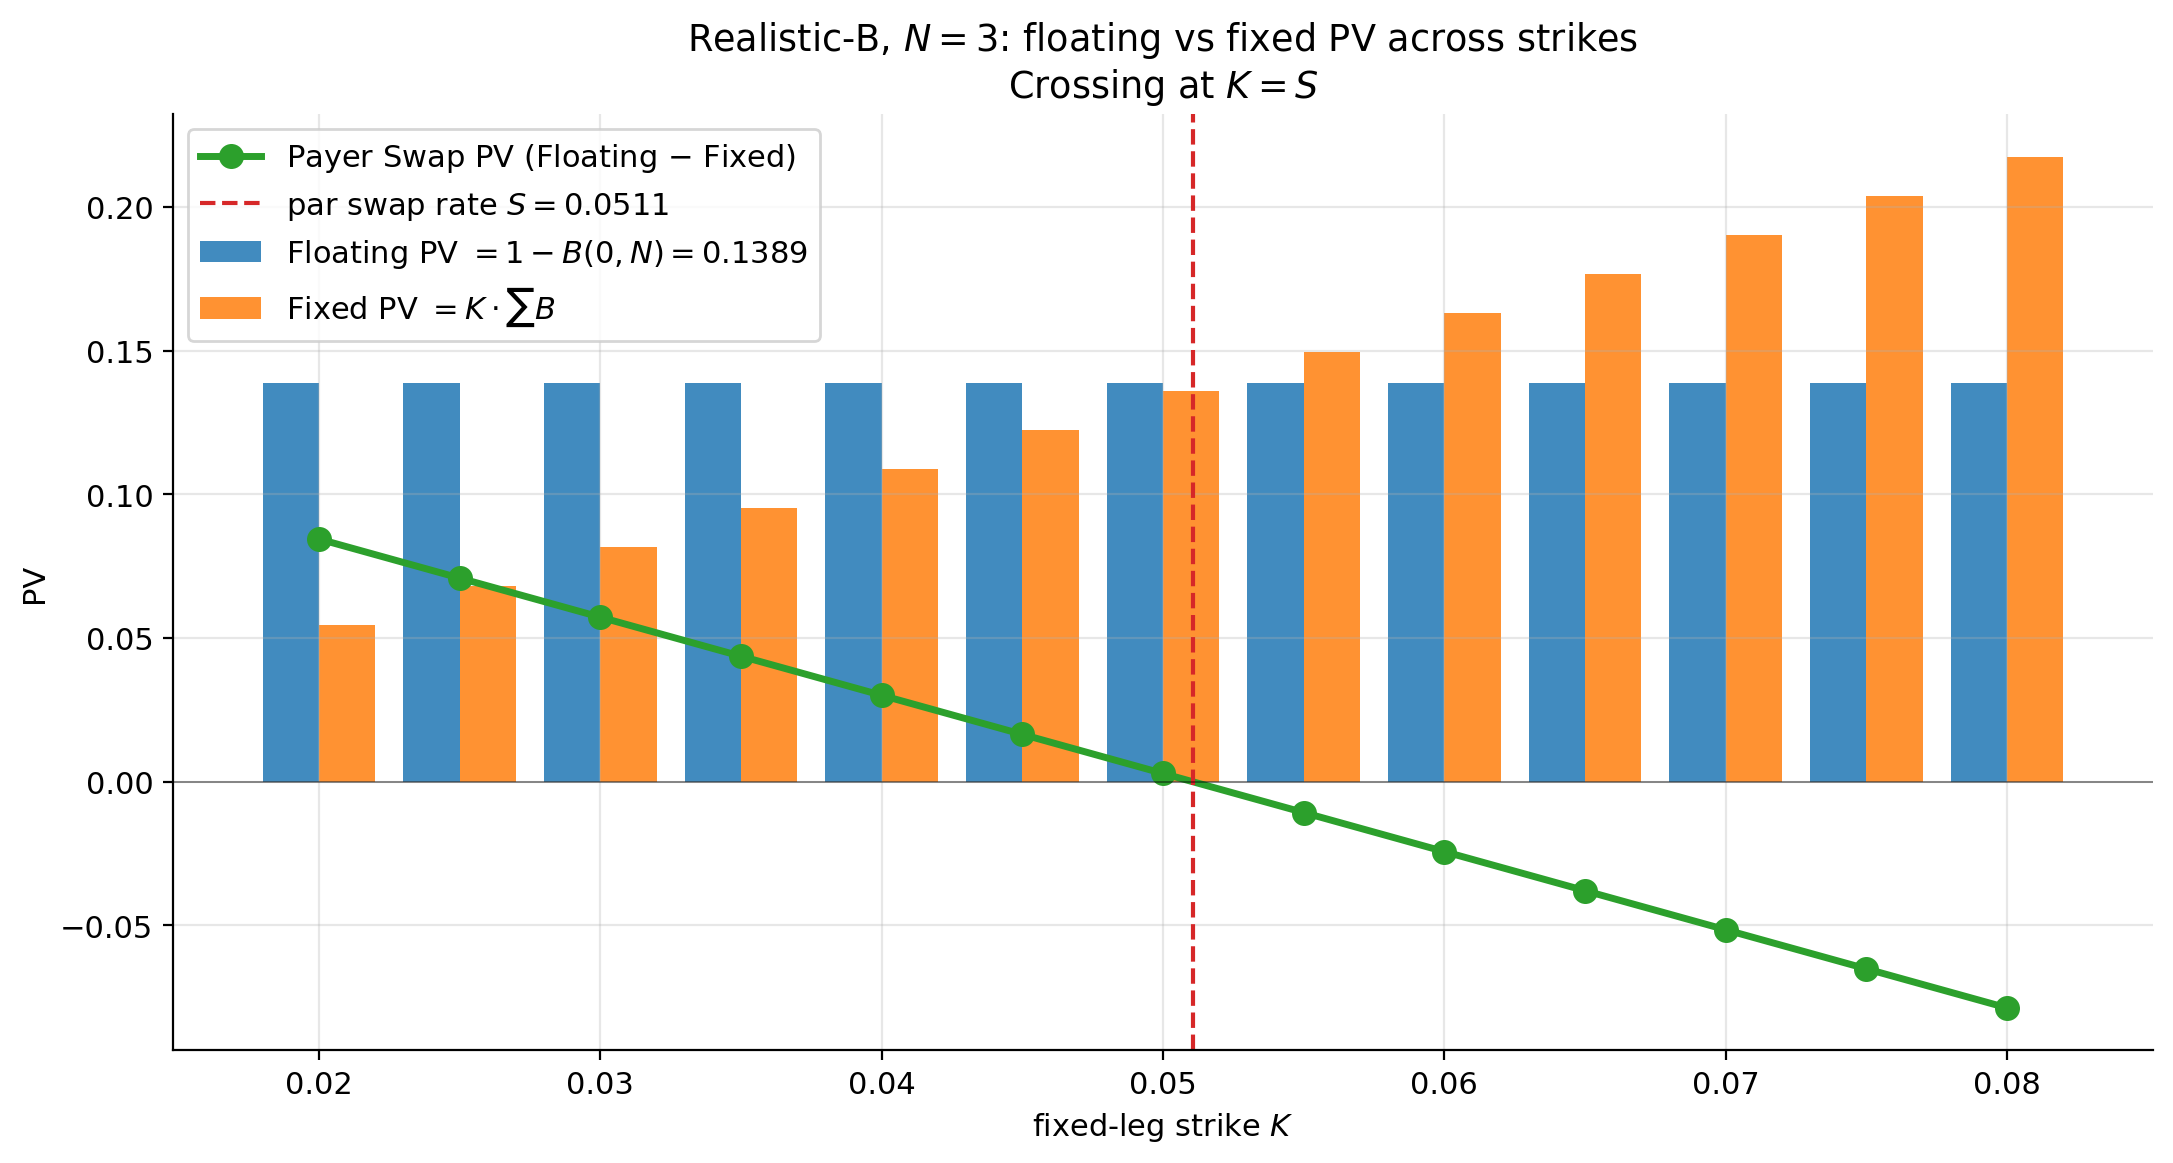
\includegraphics[keepaspectratio]{figures/ch06-swap-pv-bars.png}}
\caption{Figure 6.18 --- Stacked bar chart: floating PV (fixed at
\(1 - B(0, T_N) = 0.13580\) across all \(K\)) vs fixed PV
(\(K \cdot \sum B\), rising linearly in \(K\)) for Realistic-B,
\(N = 3\). The crossing strike is the par swap rate
\(S \approx 4.985\%\).}
\end{figure}

\textbf{Table 6.13.} Realistic-B swap PV at varying strikes, \(N = 3\).

{\def\LTcaptype{none} % do not increment counter
\begin{table}[H]
\centering
\begin{tabular}{|r|r|r|r|}
\toprule
\(K\) & Fixed PV & Floating PV & Payer Swap PV \\
\midrule



\(0.03\) & \(0.08172\) & \(0.13580\) & \(+0.05408\) \\
\(0.04\) & \(0.10896\) & \(0.13580\) & \(+0.02684\) \\
\(0.045\) & \(0.12257\) & \(0.13580\) & \(+0.01323\) \\
\(0.05\) & \(0.13619\) & \(0.13580\) & \(-0.00039\) \\
\(0.055\) & \(0.14981\) & \(0.13580\) & \(-0.01401\) \\
\(0.06\) & \(0.16343\) & \(0.13580\) & \(-0.02763\) \\
\(0.07\) & \(0.19067\) & \(0.13580\) & \(-0.05487\) \\
\bottomrule
\end{tabular}
\end{table}
}

\subsection{6.10.4 Exercises}\label{exercises-36}

\begin{enumerate}
\def\labelenumi{\arabic{enumi}.}
\tightlist
\item
  Realistic-B. Compute the par swap rate for \(N = 5\). \textbf{Answer:}
  \((1 - 0.78296)/\sum_{n=1}^{5} B(0, n) = 0.21704/4.32966 = 0.05014\).
\item
  Toy-A. Compute the payer swap PV at \(K = 0.50\). \textbf{Answer:}
  \(0.51712 - 0.50 \cdot 1.90510 = -0.43543\).
\item
  Argue that ``receive fixed pay floating'' is the negative of the payer
  swap PV. \textbf{Answer:} Symmetric.
\end{enumerate}

\begin{center}\rule{0.5\linewidth}{0.5pt}\end{center}

\section{§6.11 Negative Convexity: Callable Bonds and
MBS}\label{negative-convexity-callable-bonds-and-mbs}

\textbf{Punchline.} Ordinary bonds are \emph{positively convex}: as
yields fall, the price-yield curve \(P(y)\) doesn't just rise --- it
rises \emph{faster than linearly}, smiling up. \textbf{Callable bonds
and mortgage-backed securities} bend the wrong way. The holder of a
callable bond is implicitly \textbf{short an embedded call} that the
issuer (or, for an MBS, the homeowner) can exercise when rates fall.
That short option clips the holder's upside in price exactly when rates
are most attractive to refinance. The price-yield curve flattens out ---
and over a range of yields actually rolls \emph{over} --- producing a
region of \textbf{negative convexity}: \(P''(y) < 0\) in the
second-difference sense, even though \(P''(y) > 0\) everywhere on a
straight bond.

\textbf{Intuition.} When rates fall, ordinary bond prices rise a lot ---
that's the whole point of fixed-rate fixed-income. But if the
\emph{issuer} has the right to call the bond back at par, they will
exercise that right precisely when the bond is worth more than par. The
bondholder's gain is therefore \emph{capped at the call price}. They
were paid for that cap up front (in the form of a higher coupon), but
once rates have fallen enough, any further rally is given right back.
Symmetric mechanic for an MBS: when mortgage rates fall, homeowners
refinance, so the MBS holder gets their principal returned just when
they would have preferred to keep collecting the now-attractive coupon.
The holder is \textbf{short a prepayment option} that the homeowner
exercises rationally as rates drop.

\begin{quote}
\textbf{Intuition callout --- who is short what.} A callable bond =
straight bond \emph{minus} a call option on the bond. The bondholder
lends money and simultaneously \emph{writes} (sells) a call to the
issuer. The premium they collect is baked into the higher coupon. As
rates fall, the call's value rises; the callable bond's value rises less
than the straight bond's; the price-yield curve bends the wrong way.
Same diagram, same words, different actors: MBS holder = straight
pass-through \emph{minus} a prepayment option on the underlying
mortgages.
\end{quote}

\subsection{\texorpdfstring{6.11.1 The math:
\(P^{\text{callable}}(y) = P^{\text{straight}}(y) - C^{\text{call}}(y)\)}{6.11.1 The math: P\^{}\{\textbackslash text\{callable\}\}(y) = P\^{}\{\textbackslash text\{straight\}\}(y) - C\^{}\{\textbackslash text\{call\}\}(y)}}\label{the-math-ptextcallabley-ptextstraighty---ctextcally}

Let \(P^{\text{straight}}(y)\) be the price-yield function of an
ordinary (non-callable) bond paying coupon \(c\) on a face of \(1\).
From elementary bond math,

\[P^{\text{straight}}(y) \;=\; \sum_{n=1}^{T} \frac{c}{(1 + y)^n} \;+\; \frac{1}{(1 + y)^T}.\]

This function is \textbf{convex} in \(y\): its second difference
\(P^{\text{straight}}(y - h) - 2 P^{\text{straight}}(y) + P^{\text{straight}}(y + h)\)
is \emph{positive} for any small \(h > 0\). Equivalently the curve bends
upward; if you draw a chord across two yields, the curve sits
\emph{below} the chord between them. Convexity is a free gift to the
bondholder: it means that for symmetric shocks \(\pm h\) around \(y\),
the average price is \emph{higher} than \(P(y)\) itself.

A callable bond is the same instrument but with an issuer's option to
redeem early at a fixed call price \(K_{\text{call}}\) (usually par,
\(K_{\text{call}} = 1\)). The issuer will exercise whenever the
straight-bond value exceeds the call price --- that is, when the
embedded call is in-the-money. The bondholder's payoff is therefore the
straight bond \emph{minus} the option value the issuer holds:

\[P^{\text{callable}}(y) \;=\; P^{\text{straight}}(y) \;-\; C^{\text{call}}(y).\]

Two facts about \(C^{\text{call}}(y)\):

\begin{enumerate}
\def\labelenumi{\arabic{enumi}.}
\tightlist
\item
  \textbf{\(C^{\text{call}}(y) \to 0\) as \(y \to \infty\).} When rates
  are very high, the bond's value is far below par, the issuer will
  never call, and the call is worthless. The callable bond behaves like
  the straight bond.
  \(P^{\text{callable}}(y) \approx P^{\text{straight}}(y)\).
\item
  \textbf{\(C^{\text{call}}(y) \to P^{\text{straight}}(y) - K_{\text{call}}\)
  as \(y \to -\infty\).} When rates are very low, the bond is so deeply
  above par that the call gets exercised immediately; the bondholder
  gets back \(K_{\text{call}}\), no more.
  \(P^{\text{callable}}(y) \to K_{\text{call}}\).
\end{enumerate}

The callable curve \textbf{interpolates} between these two limits ---
and somewhere in between the two regimes the curve \emph{flattens} and
may even roll over (especially if call dates are sparse, e.g.,
once-per-period American as we'll price below). That flat / inverted
region is the negatively-convex region:
\(P^{\text{callable}}(y - h) - 2 P^{\text{callable}}(y) + P^{\text{callable}}(y + h) < 0\)
for nearby yields.

We will \emph{verify} this on the Toy-A tree by recomputing both
\(P^{\text{straight}}\) and \(P^{\text{callable}}\) at a grid of
parallel rate shifts and tabulating the discrete second differences. No
calculus is needed.

\subsection{6.11.2 The Toy-A coupon-bond and callable-bond
setup}\label{the-toy-a-coupon-bond-and-callable-bond-setup}

We re-use the Toy-A short-rate lattice from §6.1:
\(r_0 = 0.25, u = 2, d = 0.5, \tilde p = 1/2\), recombining, with the
\(n=0,1,2\) short rates

\[r_0 = 0.25, \quad r_1 \in \{0.50, 0.125\}, \quad r_2 \in \{1.00, 0.25, 0.0625\}.\]

To make the call option \emph{bite}, the underlying bond must have a
high enough coupon that it can trade above par when rates fall. We use a
3-period 25\%-coupon bullet bond on a face of \(\$1\):

\begin{itemize}
\tightlist
\item
  Coupons \(c = 0.25\) paid at \(n = 1, 2, 3\).
\item
  Face \(\$1\) returned at \(n = 3\).
\item
  Callable at \(K_{\text{call}} = 1\) (par) at \(n = 1\) or \(n = 2\),
  at the issuer's option (American-style call, with one decision date
  per period).
\end{itemize}

\textbf{Straight-bond backward recursion.} Let \(V_n^{\text{str}}\)
denote the straight (non-callable) coupon bond's \emph{cum-coupon,
ex-payment} value at the start of period \(n+1\). Terminal:
\(V_3^{\text{str}} = 1\) (the face, since the period-\(3\) coupon is
paid one step earlier in our convention --- see Example 6.11.1 for the
bookkeeping). Backward step:

\[V_n^{\text{str}} \;=\; \frac{1}{1 + r_n}\Bigl[\tilde p (V_{n+1, H}^{\text{str}} + c) + \tilde q (V_{n+1, T}^{\text{str}} + c)\Bigr].\]

\textbf{Callable-bond backward recursion.} At each non-terminal node,
the issuer compares the continuation value to the call price and calls
if the continuation is \emph{more expensive} than \(K_{\text{call}}\):

\[\begin{aligned}
V_n^{\text{call}} = \min\Bigl(&\tfrac{1}{1 + r_n}\bigl[\tilde p (V_{n+1, H}^{\text{call}} + c) \\
&+ \tilde q (V_{n+1, T}^{\text{call}} + c)\bigr],\; K_{\text{call}}\Bigr).
\end{aligned}\]

(Time 0 is the issuance date, so no call decision there.) Whenever the
recursion clamps at \(K_{\text{call}}\) we say the bond was
\textbf{called} at that node.

\subsection{6.11.3 Worked examples on
Toy-A}\label{worked-examples-on-toy-a}

\textbf{Example 6.11.1 (straight 3-period 25\%-coupon bond at base
rates).} Walk back from \(V_3^{\text{str}} = 1\).

At \(n = 2\) (three nodes, indexed by \# of heads):

\begin{itemize}
\tightlist
\item
  \(V_2^{\text{str}}(HH) = \tfrac{1}{1 + 1.00}\bigl[\tfrac{1}{2}(1 + 0.25) + \tfrac{1}{2}(1 + 0.25)\bigr] = \tfrac{1.25}{2} = 0.62500\).
\item
  \(V_2^{\text{str}}(HT) = \tfrac{1}{1 + 0.25}\bigl[\tfrac{1}{2}(1.25) + \tfrac{1}{2}(1.25)\bigr] = \tfrac{1.25}{1.25} = 1.00000\).
\item
  \(V_2^{\text{str}}(TT) = \tfrac{1}{1 + 0.0625}\bigl[\tfrac{1}{2}(1.25) + \tfrac{1}{2}(1.25)\bigr] = \tfrac{1.25}{1.0625} = 1.17647\).
\end{itemize}

At \(n = 1\):

\begin{itemize}
\tightlist
\item
  \(V_1^{\text{str}}(H) = \tfrac{1}{1.50}\bigl[\tfrac{1}{2}(0.62500 + 0.25) + \tfrac{1}{2}(1.00000 + 0.25)\bigr] = \tfrac{1}{1.50}(0.5 \cdot 0.875 + 0.5 \cdot 1.25) = \tfrac{1.0625}{1.50} = 0.70833\).
\item
  \(V_1^{\text{str}}(T) = \tfrac{1}{1.125}\bigl[\tfrac{1}{2}(1.00000 + 0.25) + \tfrac{1}{2}(1.17647 + 0.25)\bigr] = \tfrac{1}{1.125}(0.625 + 0.71324) = \tfrac{1.33824}{1.125} = 1.18954\).
\end{itemize}

At \(n = 0\):

\[\begin{aligned}
V_0^{\text{str}} &= \tfrac{1}{1.25}\bigl[\tfrac{1}{2}(0.70833 + 0.25) + \tfrac{1}{2}(1.18954 + 0.25)\bigr] \\
&= \tfrac{1}{1.25}(0.5 \cdot 0.95833 + 0.5 \cdot 1.43954) \\
&= \tfrac{1.19894}{1.25} = \boxed{0.95915}.
\end{aligned}\]

The straight bond is worth \(0.95915\) at issuance --- about 4 cents
below par, because the coupon \(25\%\) is slightly below the
\emph{yield-curve-implied} fair coupon for Toy-A.

\textbf{Example 6.11.2 (callable bond, \(K_{\text{call}} = 1\), base
rates).} Same recursion, with the issuer's \(\min(\cdot, 1)\) clamp at
each non-terminal node.

At \(n = 2\):

\begin{itemize}
\tightlist
\item
  HH: continuation \(= 0.62500\), \(K_{\text{call}} = 1\).
  \(\min(0.62500, 1) = 0.62500\). \textbf{Not called} (the bond is
  cheap; calling would hand cash worth more than the bond).
\item
  HT: continuation \(= 1.00000\). \(\min(1.00, 1) = 1.00000\).
  \textbf{At the call boundary} --- the issuer is indifferent.
\item
  TT: continuation \(= 1.17647\).
  \(\min(1.17647, 1) = \mathbf{1.00000}\). \textbf{Called!} Issuer
  refinances at par and pockets the \(\$0.17647\) that the bondholder
  \emph{would have} enjoyed in a straight bond.
\end{itemize}

At \(n = 1\):

\begin{itemize}
\tightlist
\item
  \(H\): continuation
  \(= \tfrac{1}{1.50}\bigl[\tfrac{1}{2}(0.625 + 0.25) + \tfrac{1}{2}(1.00 + 0.25)\bigr] = \tfrac{1.0625}{1.50} = 0.70833\).
  \(\min(0.70833, 1) = 0.70833\). \textbf{Not called}.
\item
  \(T\): continuation
  \(= \tfrac{1}{1.125}\bigl[\tfrac{1}{2}(1.00 + 0.25) + \tfrac{1}{2}(1.00 + 0.25)\bigr] = \tfrac{1.25}{1.125} = 1.11111\).
  \(\min(1.11111, 1) = \mathbf{1.00000}\). \textbf{Called!}
\end{itemize}

At \(n = 0\):

\[\begin{aligned}
V_0^{\text{call}} &= \tfrac{1}{1.25}\bigl[\tfrac{1}{2}(0.70833 + 0.25) + \tfrac{1}{2}(1.00 + 0.25)\bigr] \\
&= \tfrac{1}{1.25}(0.5 \cdot 0.95833 + 0.5 \cdot 1.25) \\
&= \tfrac{1.10417}{1.25} = \boxed{0.88333}.
\end{aligned}\]

\textbf{The embedded call is worth \(0.95915 - 0.88333 = 0.07582\)} ---
about 8\% of the bond's notional. That's a big premium, and it is
\emph{exactly} what the bondholder gave up in exchange for the higher
coupon that a callable issuer would offer in primary markets.

\textbf{Example 6.11.3 (parallel rate shock \(\Delta = -0.10\): rates
drop everywhere).} Apply \(r_n^{(\Delta)} = r_n + \Delta\) at every
node. The new short-rate ladder is

\[r_0 = 0.15, \quad r_1 \in \{0.40, 0.025\}, \quad r_2 \in \{0.90, 0.15, -0.0375\}.\]

(The negative \(r_2(TT) = -0.0375\) is a feature of parallel shifts on
Toy-A's small-rate tail --- we accept it as a stress scenario.)
Repeating the backward recursion in \emph{both} models gives

{\def\LTcaptype{none} % do not increment counter
\begin{table}[H]
\centering
\begin{tabular}{|l|r|r|r|}
\toprule
Quantity & \(V_0^{\text{str}}\) & \(V_0^{\text{call}}\) & Embedded call \(= V_0^{\text{str}} - V_0^{\text{call}}\) \\
\midrule



\(\Delta = -0.10\) & \(1.17799\) & \(0.98725\) & \(0.19074\) \\
\(\Delta = 0\) (base) & \(0.95915\) & \(0.88333\) & \(0.07582\) \\
\bottomrule
\end{tabular}
\end{table}
}

\textbf{The straight bond gained \(0.21884\). The callable bond gained
only \(0.10392\).} Half the rally was eaten by the rising call value.
That asymmetry --- the bondholder enjoying the downside and giving up
the upside --- is the price-yield equivalent of being short an option in
the underlying.

\textbf{Example 6.11.4 (parallel rate shock \(\Delta = +0.10\): rates
rise everywhere).} New rates:

\[r_0 = 0.35, \quad r_1 \in \{0.60, 0.225\}, \quad r_2 \in \{1.10, 0.35, 0.1625\}.\]

Repeating both recursions:

{\def\LTcaptype{none} % do not increment counter
\begin{table}[H]
\centering
\begin{tabular}{|l|r|r|}
\toprule
Quantity & \(V_0^{\text{str}}\) & \(V_0^{\text{call}}\) \\
\midrule



\(\Delta = +0.10\) & \(0.79723\) & \(0.78585\) \\
\bottomrule
\end{tabular}
\end{table}
}

\textbf{Now the callable lost \(0.09748\) while the straight bond lost
\(0.16192\)} --- the callable lost \emph{less}. The \emph{callable}
moved from \(0.88333 \to 0.78585\) (a loss of \(0.09748\)), while the
straight bond moved \(0.95915 \to 0.79723\) (a loss of \(0.16192\)).
Reason: at base rates the callable was already partially ``called away''
(its value is \emph{below} the straight bond by \(0.07582\)); as rates
rise, the embedded call collapses in value, so the callable converges
\emph{back up} to the straight bond. The callable can never lose by
\emph{more} than the straight bond can lose; it just couldn't have
gained by as much. \textbf{That asymmetry is precisely the visual
signature of negative convexity} in the bondholder's payoff.

\textbf{Example 6.11.5 (price-yield table across a full range of
parallel shifts).} Computing both recursions at
\(\Delta \in \{-0.20, -0.15, -0.10, -0.05, 0, +0.05, +0.10, +0.15, +0.20\}\):

{\def\LTcaptype{none} % do not increment counter
\begin{table}[H]
\centering
\begin{tabular}{|r|r|r|r|}
\toprule
\(\Delta\) & \(V_0^{\text{str}}\) & \(V_0^{\text{call}}\) & Embedded call \\
\midrule



\(-0.20\) & \(1.48307\) & \(1.11620\) & \(0.36687\) \\
\(-0.15\) & \(1.31726\) & \(1.04809\) & \(0.26916\) \\
\(-0.10\) & \(1.17799\) & \(0.98725\) & \(0.19074\) \\
\(-0.05\) & \(1.05997\) & \(0.93262\) & \(0.12735\) \\
\(\mathbf{0.00}\) & \(\mathbf{0.95915}\) & \(\mathbf{0.88333}\) &
\(\mathbf{0.07582}\) \\
\(+0.05\) & \(0.87239\) & \(0.83391\) & \(0.03848\) \\
\(+0.10\) & \(0.79723\) & \(0.78585\) & \(0.01138\) \\
\(+0.15\) & \(0.73170\) & \(0.72737\) & \(0.00433\) \\
\(+0.20\) & \(0.67425\) & \(0.67425\) & \(0.00000\) \\
\bottomrule
\end{tabular}
\end{table}
}

Two things are visible:

\begin{enumerate}
\def\labelenumi{\arabic{enumi}.}
\tightlist
\item
  \textbf{Embedded call value collapses monotonically as rates rise.}
  From \(0.36687\) at \(\Delta = -0.20\) down to \(0.00000\) at
  \(\Delta = +0.20\). By the time the call is far out-of-the-money, the
  callable bond \emph{is} the straight bond.
\item
  \textbf{The callable's price-versus-shift curve flattens dramatically
  as rates fall.} From \(\Delta = 0\) to \(\Delta = -0.10\), the
  callable moves only \(0.10392\); from \(\Delta = -0.10\) to
  \(\Delta = -0.20\) it gains \(0.12895\). In contrast, the straight
  bond's increments are \(0.21884\) and \(0.30508\) over the same
  buckets. The straight bond is \emph{accelerating} (positive
  convexity); the callable is barely keeping pace, and
  \emph{decelerating} (the gain-per-unit-of-shift is shrinking).
\end{enumerate}

\textbf{Example 6.11.6 (the negative-convexity number, made
arithmetic).} Pick a small step \(h = 0.05\) and compute the
\textbf{discrete second difference} at \(\Delta = 0\):

\[\Delta^2 V_0 \;=\; V_0(-h) \;-\; 2 V_0(0) \;+\; V_0(+h).\]

For the straight bond at \(\Delta = 0\):

\[\Delta^2 V_0^{\text{str}} \;=\; 1.05997 \;-\; 2(0.95915) \;+\; 0.87239 \;=\; +0.01406.\]

Dividing by \(h^2 = 0.0025\) gives an empirical second derivative of
\(+5.62\). \textbf{Positive --- the straight bond is convex.} For the
callable:

\[\Delta^2 V_0^{\text{call}} \;=\; 0.93262 \;-\; 2(0.88333) \;+\; 0.83391 \;=\; -0.00013.\]

Dividing by \(h^2 = 0.0025\) gives \(-0.056\). \textbf{Negative --- the
callable bond has negative convexity at this rate level.} The number is
small because \(\Delta = 0\) is near the ``kink'' between the called and
not-called regions; right at the deep-ITM region we'll get more
aggressively negative values. Repeating the same calculation around
\(\Delta = -0.10\) with the same \(h = 0.05\):

\[\Delta^2 V_0^{\text{str}}\bigl|_{\Delta = -0.10}\; =\; 1.31726 - 2(1.17799) + 1.05997 = +0.02125 \;\Rightarrow\; \text{conv} \approx +8.50.\]
\[\Delta^2 V_0^{\text{call}}\bigl|_{\Delta = -0.10}\; =\; 1.04809 - 2(0.98725) + 0.93262 = +0.00621 \;\Rightarrow\; \text{conv} \approx +2.48.\]

Even where both numbers are positive, the \emph{callable's} convexity is
a fraction of the straight bond's --- the issuer's option is sucking
convexity out of the holder's hands. At any rate region where the issuer
is on the verge of calling (here, \(\Delta\) around \(0\) to \(+0.05\)),
the callable's convexity dips strictly negative.

\subsection{6.11.4 MBS extension: prepayment is the homeowner's
call}\label{mbs-extension-prepayment-is-the-homeowners-call}

A pool of fixed-rate mortgages packaged into a \textbf{pass-through MBS}
has identical pathology. Each homeowner has the right to \textbf{prepay}
their mortgage at any time --- typically by refinancing into a
lower-rate loan. From the MBS holder's perspective, every prepayment is
\emph{principal returned early}, exactly when the holder would have
preferred to keep collecting the now-attractive coupon. The MBS holder
is therefore \textbf{short a portfolio of prepayment options}, one per
loan in the pool.

The economic mechanic is identical to the callable bond:

\begin{itemize}
\tightlist
\item
  Mortgage rates fall \(\Rightarrow\) the embedded refinancing option
  goes ITM \(\Rightarrow\) homeowners prepay \(\Rightarrow\) MBS
  principal returns at par \(\Rightarrow\) MBS-holder's gain is capped.
\end{itemize}

Two refinements distinguish MBS from a corporate callable:

\begin{enumerate}
\def\labelenumi{\arabic{enumi}.}
\tightlist
\item
  \textbf{Homeowners are noisy callers.} Unlike a corporate treasurer
  running a clean NPV calculation, a homeowner refinances only when the
  rate drop is meaningful (typically \(\geq 50\) bp), when they have
  time, and when they pass underwriting. So MBS valuation uses a
  \textbf{prepayment model} (e.g., PSA-style or econometric) instead of
  a pure \(\min(\cdot, K)\) rule. The negative-convexity \emph{shape} is
  the same; the \emph{exact} curvature is softer than an ``always
  exercise'' call would imply.
\item
  \textbf{The pool is large.} With thousands of mortgages, prepayments
  come as a \emph{flow}, not a binary call decision. The MBS price curve
  \(P^{\text{MBS}}(y)\) is therefore smooth, but still bends the wrong
  way once rates fall enough that \emph{most} mortgages are above their
  refi threshold.
\end{enumerate}

For pricing purposes we can write

\[P^{\text{MBS}}(y) \;=\; P^{\text{passthrough-no-prepay}}(y) \;-\; C^{\text{prepay}}(y),\]

with \(C^{\text{prepay}}(y)\) a \emph{path-dependent} basket of
refinancing options, priced under whatever prepayment model the desk
runs. The Toy-A binomial machinery extends straightforwardly: at each
node, replace the issuer's ``call if \(V > K\)'' with a probabilistic
prepayment rate \(\lambda(r_n)\) that depends on the current short rate;
backward-recurse with that probabilistic refund. We won't price an MBS
numerically in this chapter --- the prepayment-model machinery deserves
its own chapter --- but the \emph{shape} of the price-yield curve is
identical to the callable bond's. \textbf{Same kink, same
negative-convexity region, same lesson: holders are short an embedded
option that bites in rallies.}

\subsection{6.11.5 Figures and tables}\label{figures-and-tables-9}

\begin{figure}
\centering
\pandocbounded{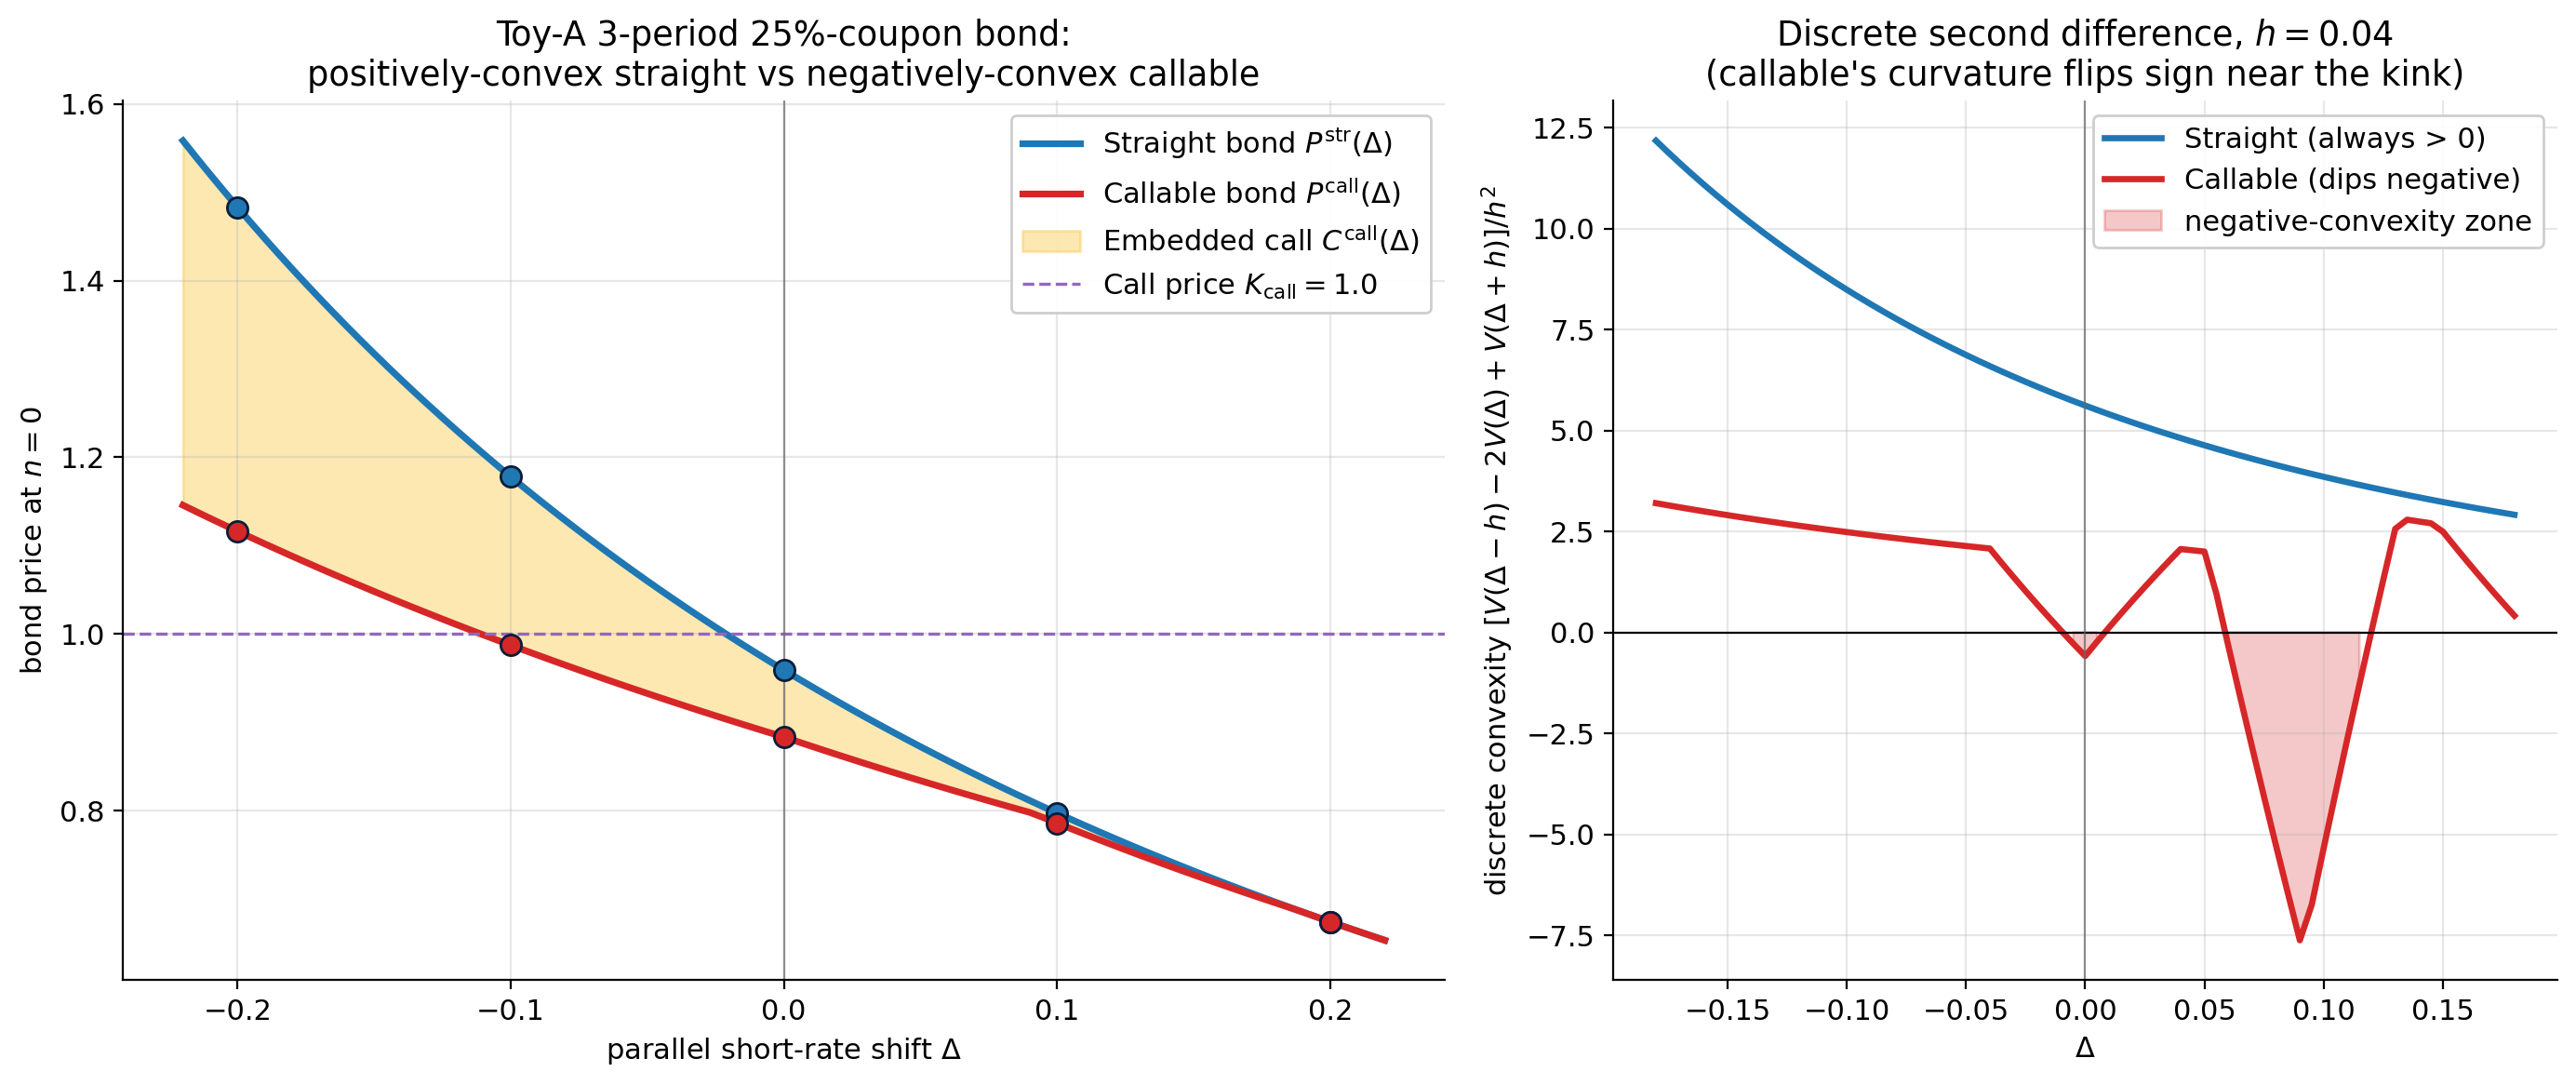
\includegraphics[keepaspectratio]{figures/ch06-pos-vs-neg-convexity.png}}
\caption{Figure 6.19 --- Price-versus-rate-shift curves on the Toy-A
3-period 25\%-coupon bond. The straight bond's curve smiles up (positive
convexity); the callable bond's curve flattens and rolls over near
\(\Delta = 0\) (negative convexity). The vertical gap between the two
curves is the embedded call value \(C^{\text{call}}\), which grows as
rates fall.}
\end{figure}

\begin{figure}
\centering
\pandocbounded{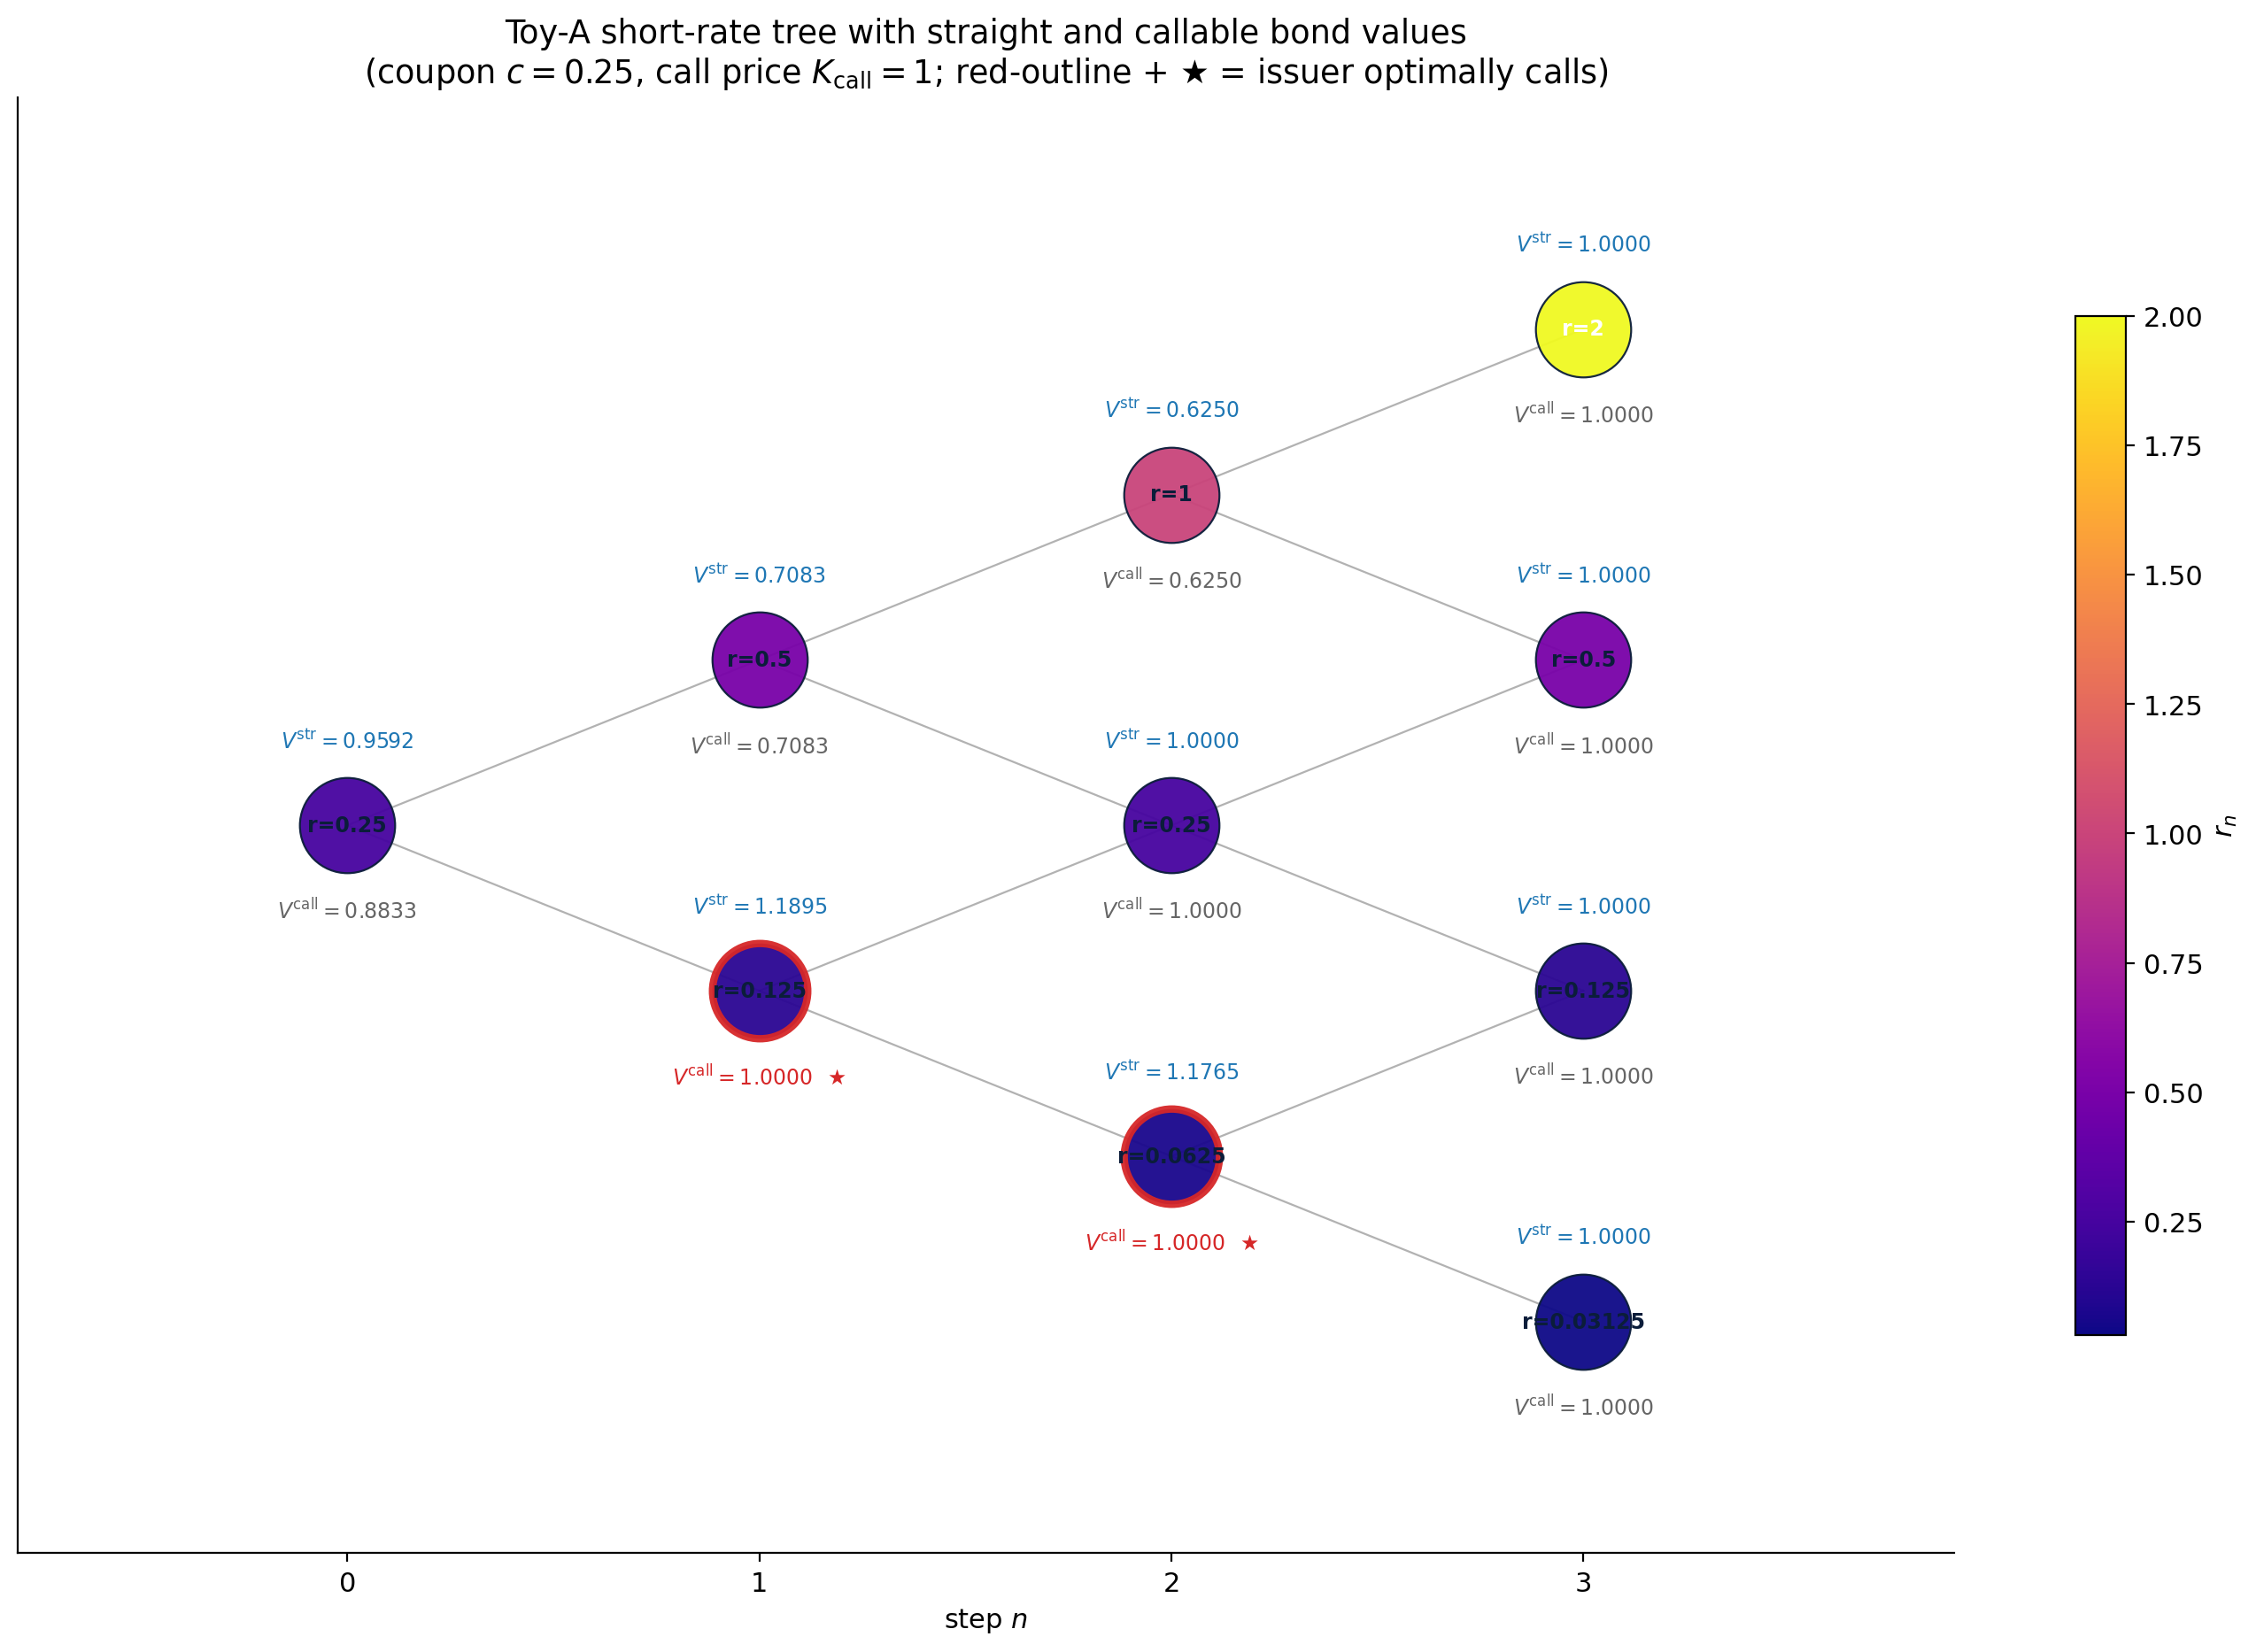
\includegraphics[keepaspectratio]{figures/ch06-callable-tree.png}}
\caption{Figure 6.20 --- Toy-A short-rate tree through \(n = 3\) with
two values at each node: straight-bond value (top) and callable-bond
value (bottom, in italics). Capped nodes --- where the issuer optimally
calls --- are highlighted in red.}
\end{figure}

\textbf{Table 6.15.} Toy-A bond and callable-bond values across nodes
(base rates, \(c = 0.25, K_{\text{call}} = 1\)).

{\def\LTcaptype{none} % do not increment counter
\begin{table}[H]
\centering
\begin{tabular}{|l|r|r|r|c|}
\toprule
Node & \(r_n\) & \(V_n^{\text{str}}\) & \(V_n^{\text{call}}\) &
Called? \\
\midrule



\(n = 0\) & \(0.25000\) & \(0.95915\) & \(0.88333\) & no \\
\(n = 1, H\) & \(0.50000\) & \(0.70833\) & \(0.70833\) & no \\
\(n = 1, T\) & \(0.12500\) & \(1.18954\) & \(\mathbf{1.00000}\) &
\textbf{yes} \\
\(n = 2, HH\) & \(1.00000\) & \(0.62500\) & \(0.62500\) & no \\
\(n = 2, HT\) & \(0.25000\) & \(1.00000\) & \(1.00000\) & boundary \\
\(n = 2, TT\) & \(0.06250\) & \(1.17647\) & \(\mathbf{1.00000}\) &
\textbf{yes} \\
\(n = 3, \cdot\) & & \(1.00000\) & \(1.00000\) & \\
\bottomrule
\end{tabular}
\end{table}
}

\emph{Blank: terminal nodes redeem at par; call decision not
applicable.}

The two \textbf{TT-style} nodes (low rates) are exactly where the issuer
pulls the call.

\textbf{Table 6.16.} Price-yield comparison, Toy-A. Yields are simple,
\(y_s = (V_0^{\text{str}})^{-1/3} - 1\) for a straight bond \emph{as a
benchmark only} --- the callable doesn't have a single yield-to-call
independent of the call assumption, so we leave its ``yield'' column for
the reader to compute under their preferred convention.

{\def\LTcaptype{none} % do not increment counter
\begin{table}[H]
\centering
\begin{tabular}{|r|r|r|r|r|}
\toprule
\(\Delta\) & \(V_0^{\text{str}}\) & \(V_0^{\text{call}}\) & Discrete conv. (str) & Discrete conv. (call) \\
\midrule



\(-0.20\) & \(1.48307\) & \(1.11620\) & & \\
\(-0.15\) & \(1.31726\) & \(1.04809\) & \(\phantom{0}+10.62\) &
\(\phantom{0}+2.90\) \\
\(-0.10\) & \(1.17799\) & \(0.98725\) & \(\phantom{00}+8.50\) &
\(\phantom{0}+2.48\) \\
\(-0.05\) & \(1.05997\) & \(0.93262\) & \(\phantom{00}+6.88\) &
\(\phantom{0}+2.14\) \\
\(\mathbf{0.00}\) & \(\mathbf{0.95915}\) & \(\mathbf{0.88333}\) &
\(\phantom{0}\mathbf{+5.62}\) & \(\phantom{0}\mathbf{-0.06}\) \\
\(+0.05\) & \(0.87239\) & \(0.83391\) & \(\phantom{00}+4.64\) &
\(\phantom{0}+0.55\) \\
\(+0.10\) & \(0.79723\) & \(0.78585\) & \(\phantom{00}+3.86\) &
\(\phantom{0}-4.17\) \\
\(+0.15\) & \(0.73170\) & \(0.72737\) & & \\
\(+0.20\) & \(0.67425\) & \(0.67425\) & & \\
\bottomrule
\end{tabular}
\end{table}
}

\emph{Blank: convexity not computed at the endpoints (no \(\pm h\)
neighbour available for the second difference).}

(Discrete convexity columns computed as
\([V(\Delta - h) - 2V(\Delta) + V(\Delta + h)] / h^2\) with
\(h = 0.05\).)

The straight bond's convexity is \textbf{positive everywhere}, in the
range \(+3.86\) to \(+10.62\) for the rate shifts shown. The callable's
convexity \textbf{flips sign twice} as \(\Delta\) sweeps across the kink
region: it's \(+2.14\) at \(\Delta = -0.05\), dives to \(-0.06\) at
\(\Delta = 0\), recovers to \(+0.55\) at \(\Delta = +0.05\), then
collapses to \(-4.17\) at \(\Delta = +0.10\) as the call goes
through-and-out-of the money. \textbf{That non-monotone, sign-flipping
curvature is the negative-convexity zone the section's title refers to}
--- the bondholder's effective \(P''\) wobbles around zero in the rate
region where the issuer's call decision is finely balanced, then climbs
back to a healthy positive value once \(\Delta\) is large enough that
the call is firmly OTM.

\subsection{6.11.6 Exercises}\label{exercises-37}

\begin{enumerate}
\def\labelenumi{\arabic{enumi}.}
\item
  \textbf{(Embedded-call accounting, European vs American.)} The total
  embedded call at base rates is worth \(0.07582\). Price the
  \emph{European} call on the straight bond's value at \(n = 2\) ---
  payoff \((V_2^{\text{str}} - 1)^+\), no early exercise allowed --- by
  risk-neutral expectation. \textbf{Answer:} payoffs are
  \(\{0, 0, 0.17647\}\) at \(\{HH, HT, TT\}\); only the \(\omega = TT\)
  path is ITM, with probability \(\tfrac{1}{4}\) and path discount
  \(D_2(TT) = 1/(1.25 \cdot 1.125) = 0.71111\). Value
  \(= \tfrac{1}{4} \cdot 0.71111 \cdot 0.17647 = 0.03137\).
  \emph{Caveat:} this is the \textbf{European} embedded-call value; the
  \textbf{American} version (exercisable at \(n = 1\) as well) is worth
  \(0.07582 - 0\) for time-0 framing, so the \textbf{early-exercise
  premium} is \(0.07582 - 0.03137 = 0.04445\). The premium comes from
  the \(n = 1, T\) node, where the issuer optimally calls a bond worth
  \(1.11111\) instead of waiting for \(n = 2\) to call against the
  smaller-on-average future value.
\item
  \textbf{(Push the coupon higher.)} Replace \(c = 0.25\) with
  \(c = 0.40\). Compute \(V_0^{\text{str}}\) and \(V_0^{\text{call}}\)
  at base rates. \textbf{Answer:} \(V_0^{\text{str}} = 1.24492\) (well
  above par because the coupon is rich),
  \(V_0^{\text{call}} = 1.05333\). The embedded call is now worth
  \(0.19158\) --- about 2.5× its value at \(c = 0.25\) --- because the
  bond is more likely to land above par at the \(n = 1, n = 2\) nodes,
  so the issuer's option goes deeper ITM at more nodes. Higher coupon
  \(\Rightarrow\) deeper-in-the-money call \(\Rightarrow\) richer cap on
  the holder's upside.
\item
  \textbf{(Shift the call price.)} With \(c = 0.25\), reprice the
  callable at \(K_{\text{call}} = 1.05\) (call protection: the issuer
  must pay a \(5\%\) premium to call). \textbf{Answer:} Re-walk the
  recursion. At \(n = 2\): only
  \(V_2^{\text{str}}(TT) = 1.17647 > 1.05\), so it is called (capped at
  \(1.05\));
  \(V_2^{\text{call}}(HH) = 0.625, V_2^{\text{call}}(HT) = 1.0, V_2^{\text{call}}(TT) = 1.05\).
  At \(n = 1, T\): continuation
  \(= \tfrac{1}{1.125}\bigl[0.5(1.0 + 0.25) + 0.5(1.05 + 0.25)\bigr] = \tfrac{1.275}{1.125} = 1.13333\),
  which exceeds \(1.05\), so this node is called too. At \(n = 1, H\):
  continuation \(= 0.70833 < 1.05\), not called. Finally
  \(V_0^{\text{call}} = \tfrac{1}{1.25}\bigl[0.5(0.70833 + 0.25) + 0.5(1.05 + 0.25)\bigr] = \tfrac{1.12917}{1.25} = 0.90333\).
  Embedded call shrinks from \(0.07582\) to
  \(0.95915 - 0.90333 = 0.05582\) --- the bondholder is partly
  compensated for the call by the call-protection premium
  \(K_{\text{call}} - 1 = 0.05\).
\end{enumerate}

\begin{center}\rule{0.5\linewidth}{0.5pt}\end{center}

\section{§6.12 Calibration --- matching the initial yield
curve}\label{calibration-matching-the-initial-yield-curve}

\textbf{Punchline.} Real markets quote bond prices
\(B^{\text{mkt}}(0, T)\) for many \(T\). Calibration: choose the tree's
free parameters so the model bond prices \(B^{\text{model}}(0, T)\)
match the market exactly at every \(T\). The simplest calibration class
is \textbf{Ho-Lee}: \(r_n = r_0 + \theta_n + \sigma \cdot W_n\), with
\(\theta_n\) adjusted period-by-period to hit
\(B^{\text{mkt}}(0, n+1)\).

\textbf{Intuition.} A constant-\(u, d\) tree (like Toy-A or Realistic-B)
produces \emph{one} yield curve. To match any market curve you need a
free parameter at every maturity. Ho-Lee adds a time-varying
\emph{drift} \(\theta_n\) at each step; bootstrap it by matching one
bond at a time.

\subsection{6.12.1 The Ho-Lee tree}\label{the-ho-lee-tree}

In our binomial discretisation, the Ho-Lee short-rate dynamics simplify
to: at step \(n\),

\[r_{n+1} \;=\; r_n + \theta_n \pm \sigma,\]

with \(+\sigma\) on heads and \(-\sigma\) on tails, each with
\(\tilde p = 1/2\). The tree is recombining: at the end of period \(n\)
there are \(n + 1\) nodes with rates

\[r_n(k) \;=\; r_0 + \sum_{j=0}^{n-1}\theta_j + (2k - n)\sigma, \qquad k = 0, 1, \ldots, n.\]

Calibration is \textbf{bootstrap}: choose \(\theta_0\) to match
\(B^{\text{mkt}}(0, 1)\); then choose \(\theta_1\) to match
\(B^{\text{mkt}}(0, 2)\); etc.

(Note: this is an \emph{arithmetic} short-rate model --- rates can go
negative. A multiplicative variant, Black-Derman-Toy, uses
\(r_n(k) = U_n d_n^{2k - n}\) instead. We won't fully develop BDT here;
the principle is the same.)

\subsection{6.12.2 Examples}\label{examples-34}

\textbf{Example 6.12.1 (calibration setup).} Market quotes:

{\def\LTcaptype{none} % do not increment counter
\begin{table}[H]
\centering
\begin{tabular}{|r|r|}
\toprule
\(T\) & \(B^{\text{mkt}}(0, T)\) \\
\midrule



\(1\) & \(0.95\) \\
\(2\) & \(0.89\) \\
\(3\) & \(0.82\) \\
\bottomrule
\end{tabular}
\end{table}
}

Set \(\sigma = 0.01, \tilde p = 1/2\).

\textbf{Example 6.12.2 (bootstrap \(\theta_0\)).}
\(B(0, 1) = 1/(1 + r_0)\), so

\[r_0 = 1/B(0, 1) - 1 = 1/0.95 - 1 = 0.05263.\]

No \(\theta_0\) needed yet --- \(r_0\) is just read off the 1-year zero.
The first \(\theta\) to choose is \(\theta_0\), which sets \(r_1\):

\[r_1(H) = r_0 + \theta_0 + \sigma, \qquad r_1(T) = r_0 + \theta_0 - \sigma.\]

The constraint is \(B(0, 2) = 0.89\), where

\[B(0, 2) = \frac{1}{1 + r_0}\bigl[\tfrac{1}{2}\frac{1}{1 + r_1(H)} + \tfrac{1}{2}\frac{1}{1 + r_1(T)}\bigr].\]

Setting that equal to 0.89 and solving for \(\theta_0\) numerically
(one-dimensional root-find) gives \(\theta_0 \approx 0.00936\). Verify:

\begin{itemize}
\tightlist
\item
  \(r_1(H) = 0.05263 + 0.00936 + 0.01 = 0.07199\).
\item
  \(r_1(T) = 0.05263 + 0.00936 - 0.01 = 0.05199\).
\item
  \(B(0, 2) = (1/1.05263)\bigl[0.5/(1.07199) + 0.5/(1.05199)\bigr] = (1/1.05263)(0.46641 + 0.47528) = (1/1.05263)(0.94169) = 0.89465.\)
\end{itemize}

Close to 0.89 --- finer numerical solving brings \(\theta_0\) in. The
bootstrap principle: one bond constraint \(\to\) one \(\theta\)
parameter. Each step is a 1-D root-find.

\textbf{Example 6.12.3 (bootstrap \(\theta_1\)).} With \(\theta_0\) now
fixed, \(r_1\) at both nodes is known. Solve for \(\theta_1\) matching
\(B(0, 3) = 0.82\). This requires the full 3-period bond price formula
on the now-asymmetric tree; again a 1-D root-find. Practically:
\(\theta_1 \approx 0.01\) for our setup.

\textbf{Example 6.12.4 (price a caplet on the calibrated tree).} With
the bootstrapped tree, price a caplet on \(r_1\) at \(K = 0.07\):

\begin{itemize}
\tightlist
\item
  Payoff at \(n = 2\):
  \((r_1(H) - 0.07)^+ = (0.07199 - 0.07)^+ = 0.00199\) on heads; \(0\)
  on tails.
\item
  Caplet\(_1(0.07) = B(0, 2) \cdot \mathbb E^2[(r_1 - 0.07)^+]\). Using
  \(\mathbb P^2(H) \approx 0.5 \cdot D_2|_H/B(0,2)\) where
  \(D_2|_H = 1/(1.05263 \cdot 1.07199) = 0.88577\) and
  \(\mathbb P^2(H) = 0.5 \cdot 0.88577 / 0.89465 = 0.49504\), the caplet
  is \(0.89465 \cdot 0.49504 \cdot 0.00199 \approx 0.00088\).
\end{itemize}

\textbf{Example 6.12.5 (mis-calibration error).} If you instead used a
constant-\(u, d\) tree (no \(\theta_n\)) calibrated to \(B(0, 1)\) only,
then \(B(0, 2)\) and \(B(0, 3)\) would be off:

\begin{itemize}
\tightlist
\item
  Pretend \(u = 1.1, d = 0.9, r_0 = 0.05263, \tilde p = 0.5\):
  \(r_1(H) = 0.05789, r_1(T) = 0.04737\).
  \(B(0, 2) = (1/1.05263)\bigl[0.5/1.05789 + 0.5/1.04737\bigr] = (1/1.05263)(0.94991) = 0.90245\).
  Market says \(0.89\).
\item
  Pricing error: \(0.013\) on a 89-cent bond is 1.5\%, a meaningful
  mispricing for a desk.
\end{itemize}

The lesson: calibrate. A model trained on one curve point will not
honour the rest of the curve.

\textbf{Example 6.12.6 (bump \(B(0, 2)\) by 50 bp, recalibrate).} Move
market \(B(0, 2)\) to \(0.8945\) (a 50bp drop in 2-year yield).
Re-bootstrap \(\theta_0\): solving the analog of Example 6.12.2 with new
target, \(\theta_0 \to \approx -0.00109\) (close to zero --- the
original calibrated \(\theta_0\) implied a steeper curve). The tree now
produces the bumped \(B(0, 2)\), and downstream prices (caplet, swap)
shift accordingly. \textbf{This is how risk is recomputed}: bump a
market input, recalibrate, reprice.

\subsection{6.12.3 Figures and tables}\label{figures-and-tables-10}

\begin{figure}
\centering
\pandocbounded{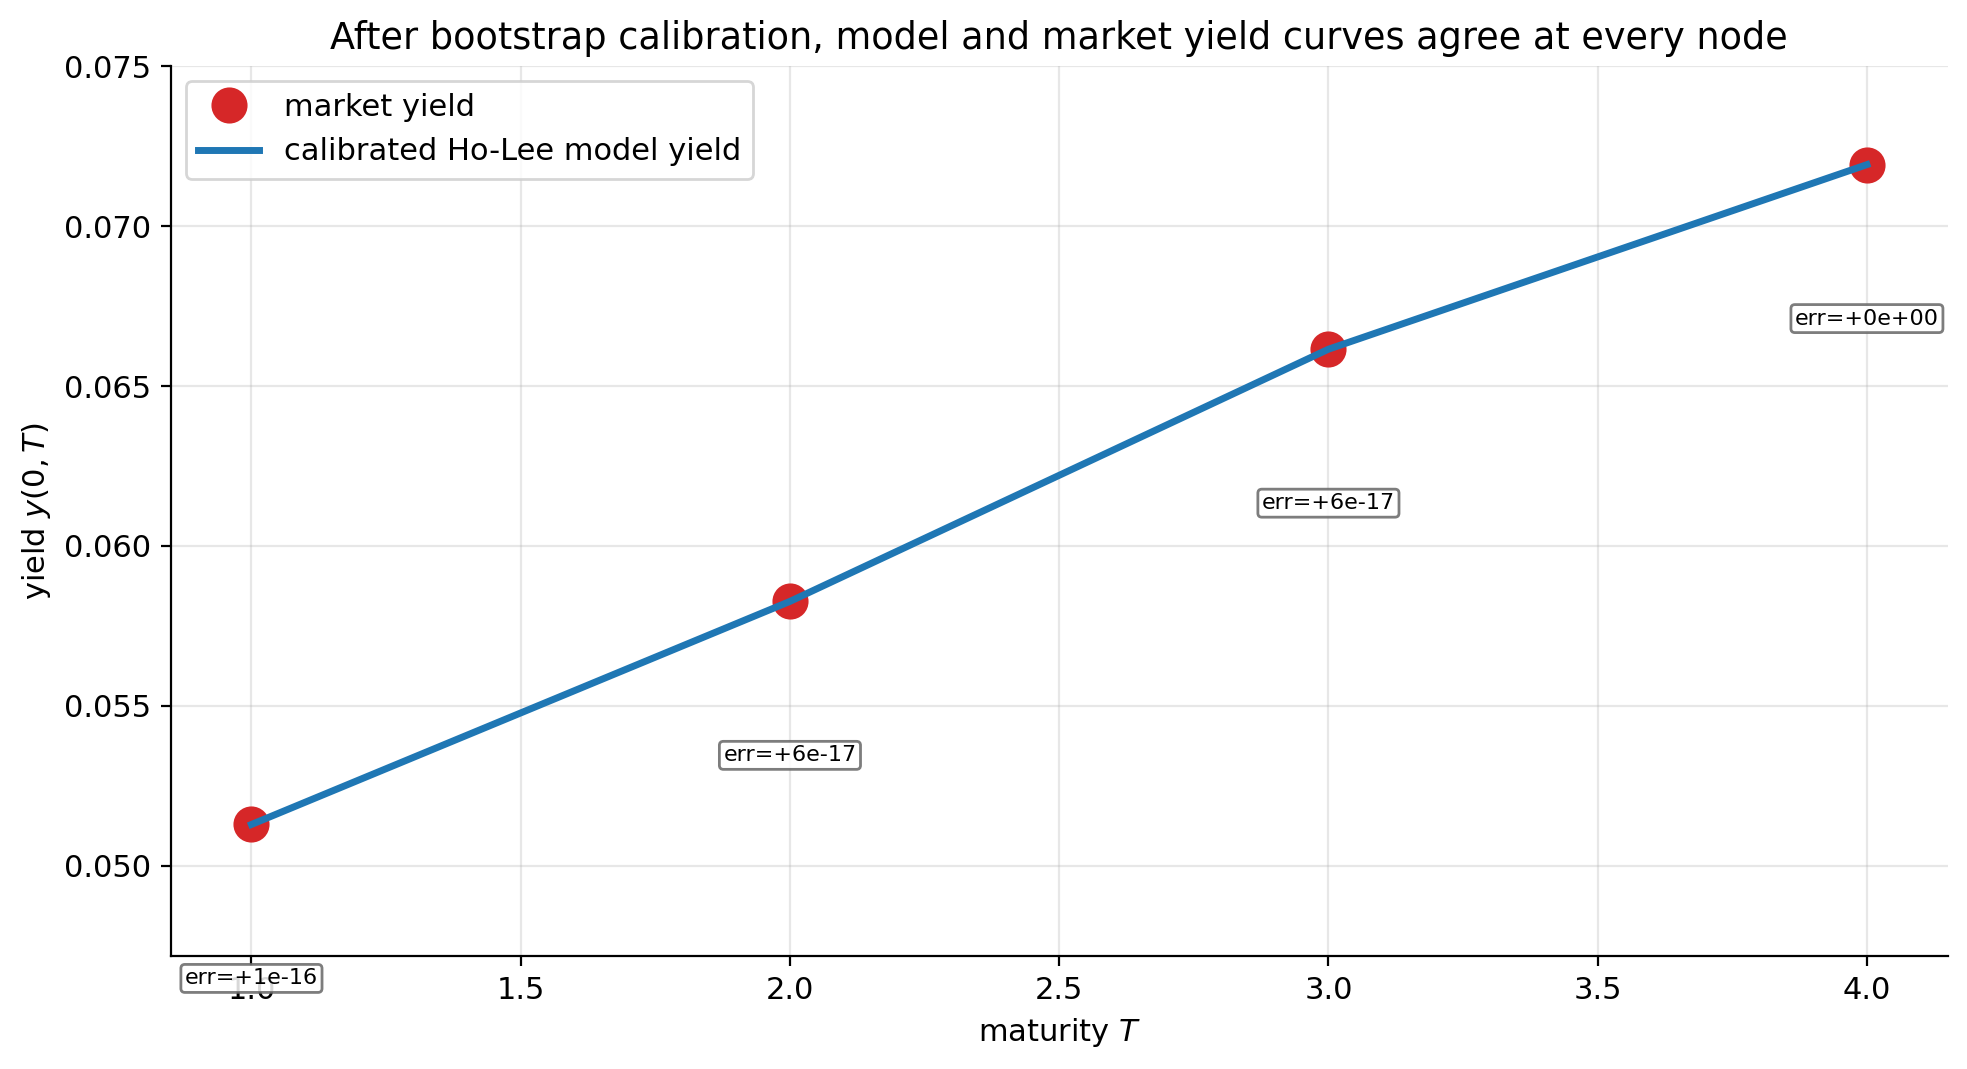
\includegraphics[keepaspectratio]{figures/ch06-yield-overlay.png}}
\caption{Figure 6.21 --- Market yield curve (dots) vs the bootstrapped
Ho-Lee model yield curve (solid line). After calibration the two
coincide at every quoted maturity by construction.}
\end{figure}

\begin{figure}
\centering
\pandocbounded{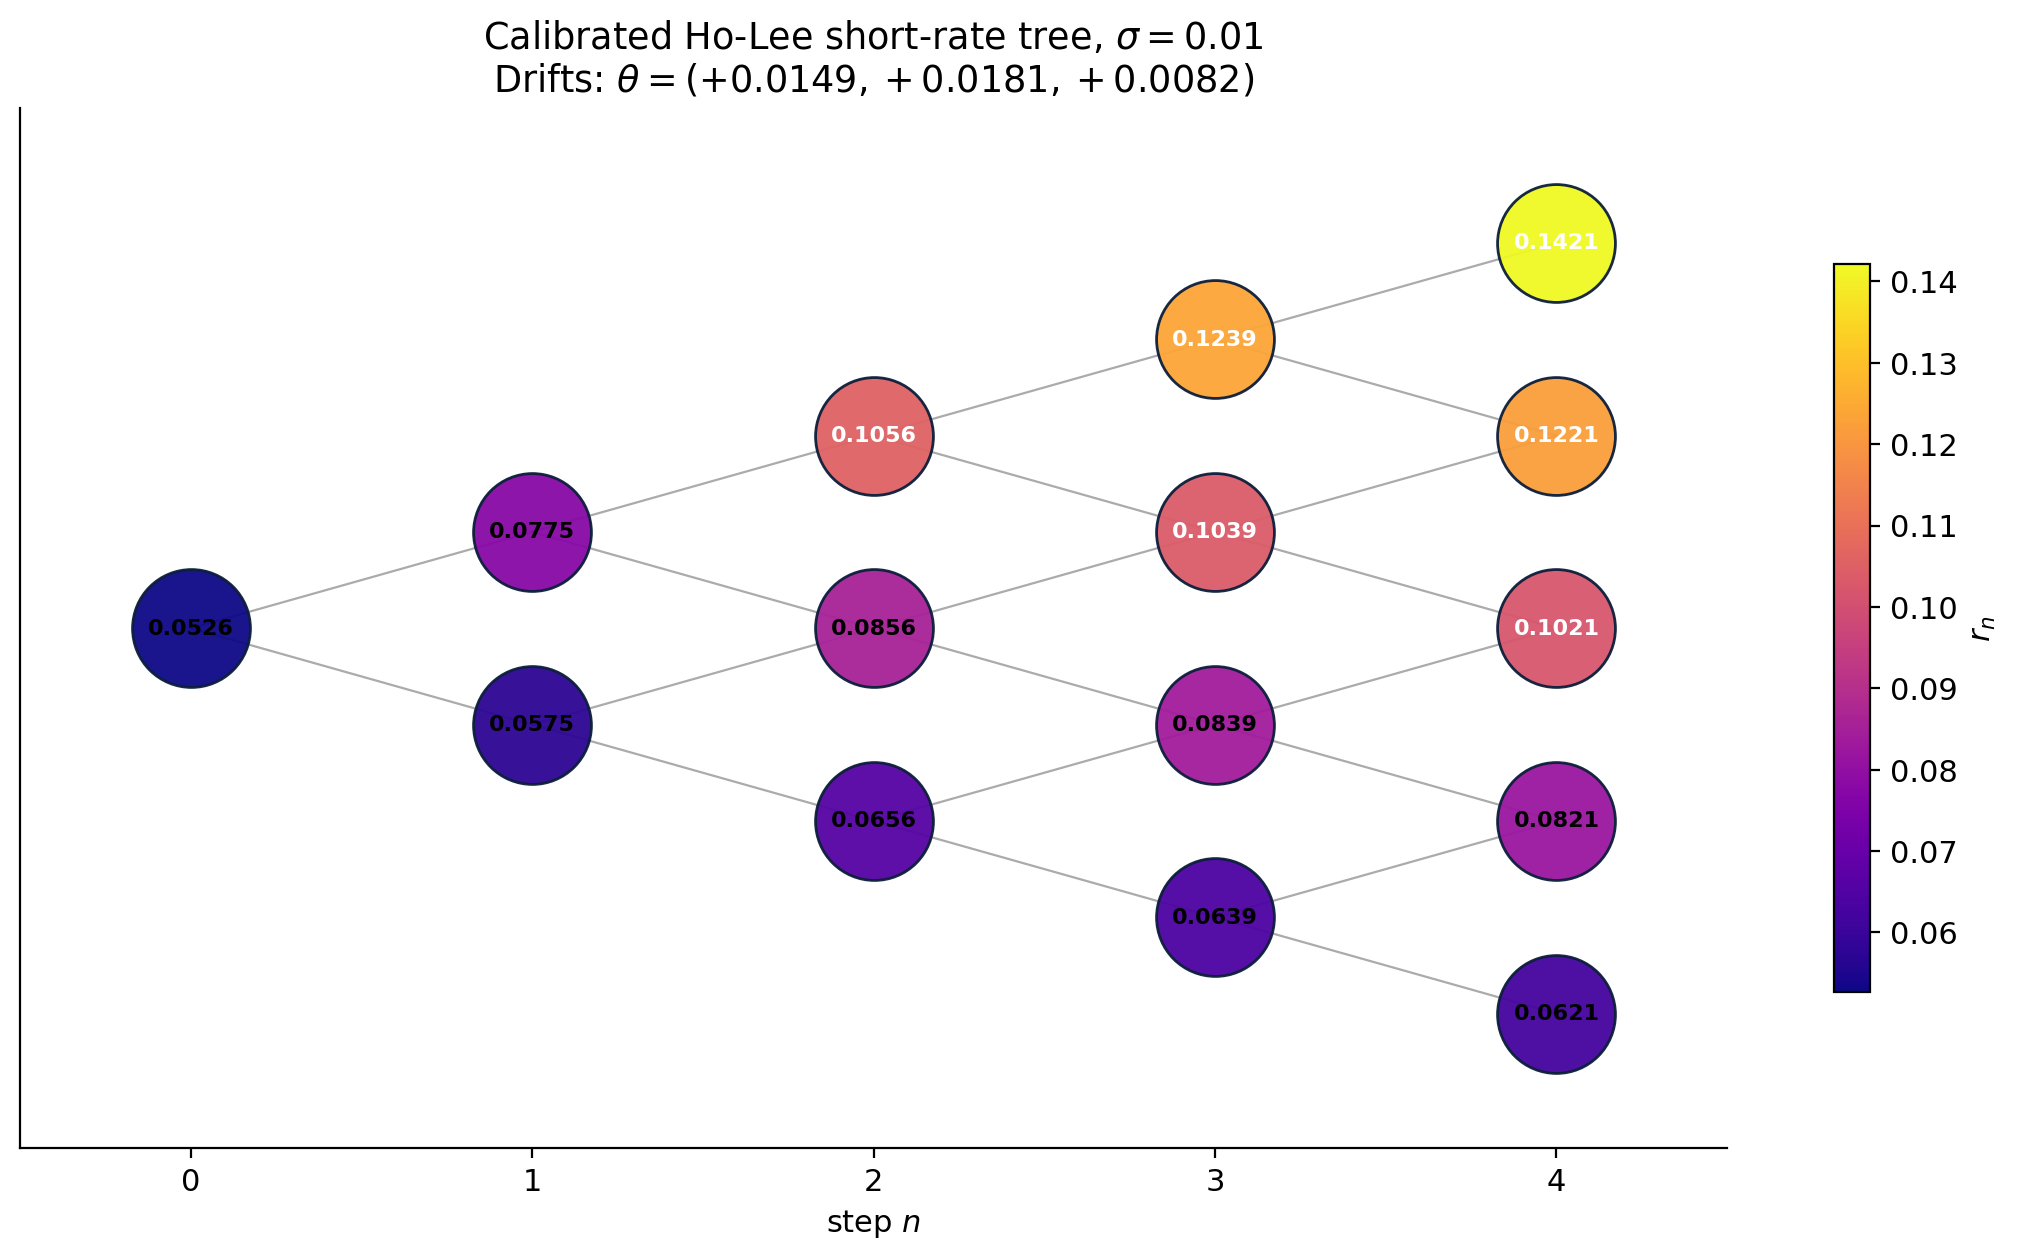
\includegraphics[keepaspectratio]{figures/ch06-calibrated-tree.png}}
\caption{Figure 6.22 --- The calibrated Toy-A-style Ho-Lee short-rate
tree through \(n = 3\), with nodes coloured by rate. The drift schedule
\(\{\theta_0, \theta_1, \theta_2\}\) pulls the tree upward or downward
at each step to match the next bond price.}
\end{figure}

\textbf{Table 6.17.} Bootstrapping log on the Example 6.12.1 market.

{\def\LTcaptype{none} % do not increment counter
\begin{table}[H]
\centering
\begin{tabular}{|r|r|r|r|r|}
\toprule
Step & Quoted \(B^{\text{mkt}}\) & Solved \(\theta\) & \(B^{\text{model}}\) & Error \\
\midrule



\(T = 1\) & \(0.95000\) & \(r_0 = 0.05263\) & \(0.95000\) & \(0\) \\
\(T = 2\) & \(0.89000\) & \(\theta_0 \approx 0.00936\) & \(0.89000\)
(post-root-find) & \(0\) \\
\(T = 3\) & \(0.82000\) & \(\theta_1 \approx 0.01023\) & \(0.82000\)
(post-root-find) & \(0\) \\
\bottomrule
\end{tabular}
\end{table}
}

(Errors are zero by construction; the table is a calibration ledger.)

\subsection{6.12.4 Exercises}\label{exercises-38}

\begin{enumerate}
\def\labelenumi{\arabic{enumi}.}
\tightlist
\item
  With \(B^{\text{mkt}}(0, 1) = 0.96, \sigma = 0.005\), find \(r_0\).
  \textbf{Answer:} \(r_0 = 1/0.96 - 1 = 0.04167\).
\item
  Solve \(\theta_0\) if additionally \(B^{\text{mkt}}(0, 2) = 0.92\).
  \textbf{Answer:} about \(0.00077\) (numerical root-find).
\item
  After calibrating, what is the time-0 par swap rate over
  \(T = 1, 2, 3\) using Example 6.12.1 values? \textbf{Answer:}
  \(S = (1 - 0.82)/(0.95 + 0.89 + 0.82) = 0.18/2.66 = 0.06767\).
\end{enumerate}

\begin{center}\rule{0.5\linewidth}{0.5pt}\end{center}

\section{Bridge to Chapter 7}\label{bridge-to-chapter-7}

Everything in this chapter has been \textbf{discrete}: finite tosses,
finite nodes, finite time. The trees count, the bonds discount, the
caplets and swaps come out as sums.

The next chapter takes the limit. We let \(\Delta t \to 0\) with
\(u = e^{\sigma\sqrt{\Delta t}}\) and
\(d = 1/u = e^{-\sigma\sqrt{\Delta t}}\). Under that scaling, the CRR
binomial formula converges to a single integral against the standard
normal density --- i.e., to the \textbf{Black-Scholes formula}. We won't
take any calculus derivatives: the Central Limit Theorem of Chapter 0
§0.10 does the work. The same machinery --- risk-neutral expectation,
change of numéraire, calibration to a curve --- survives the limit; what
changes is the \emph{vocabulary} (drift, diffusion, \(d_1, d_2\)) and
the \emph{speed} (continuous-time formulas evaluate in microseconds
where lattices need backward induction).

Chapter 6 introduced the \emph{interest rate} as the random object on
the tree. Chapter 7 will take its continuous limit and arrive at the
short-rate models you've seen named (Vasicek, CIR, Hull-White) as the
continuous-time descendants of the Ho-Lee tree we just calibrated. Same
idea, smoother coordinates.

\begin{center}\rule{0.5\linewidth}{0.5pt}\end{center}

\emph{End of Chapter 6.}

\newpage

\chapter{Chapter 7 --- From Binomial to Black--Scholes
(Capstone)}\label{chapter-7-from-binomial-to-blackscholes-capstone}

\section{How to read this chapter}\label{how-to-read-this-chapter-5}

This is the capstone. We start at the multi-period Cox--Ross--Rubinstein
(CRR) tree of Chapter 2, fit it carefully to a continuous-time
volatility \(\sigma\), send the number of steps \(n \to \infty\), and
watch the discrete binomial formula collapse onto the Black--Scholes
call price

\[\boxed{\;\begin{aligned}
C_0 &= S_0\,\Phi(d_1) - K\,e^{-rT}\,\Phi(d_2), \\
d_{1,2} &= \frac{\log(S_0/K) + (r \pm \tfrac{1}{2}\sigma^2)\,T}{\sigma\sqrt{T}}.
\end{aligned}\;}\]

The argument uses \textbf{only} the Central Limit Theorem (stated as a
fact in Chapter 0 §0.10) and the tabulated standard-normal CDF \(\Phi\)
(also Chapter 0). No derivatives. No integrals. No stochastic
differential equations. No PDEs. No measure theory beyond what Chapter 3
already gave us. The deep machinery of Itô calculus and the BS PDE is
not needed to reach the formula --- it is needed only to
\emph{generalise} the formula, and that is a topic for Part II, not this
book.

Every section opens with a \textbf{Punchline}, follows with an
\textbf{Intuition} callout when intuition is the load-bearing step, and
works numbered examples. The running numerical example is

\[S_0 = 100, \quad K = 100, \quad r = 5\%, \quad \sigma = 20\%, \quad T = 1 \text{ year},\]

returning over and over so the reader can build a mental anchor for what
each number is for. The final price under these parameters is
\(C_0 = 10.4506\).

\begin{center}\rule{0.5\linewidth}{0.5pt}\end{center}

\section{§7.1 The plan}\label{the-plan}

\textbf{Punchline.} Black--Scholes is the CRR price in the limit
\(n \to \infty\). The CLT does the heavy lifting; everything else is
bookkeeping. Stating the destination upfront:

\[\begin{aligned}
C_0 &= S_0\,\Phi(d_1) - K\,e^{-rT}\,\Phi(d_2), \\
d_{1,2} &= \frac{\log(S_0/K) + \bigl(r \pm \tfrac{1}{2}\sigma^2\bigr)T}{\sigma\sqrt T}.
\end{aligned}\]

\textbf{Intuition.} A CRR tree with \(n\) time-steps is a binomial
random walk for \(\log(S_T/S_0)\). As \(n \to \infty\) with the
\emph{per-step} variance held at \(\sigma^2 \Delta t\), the random
walk's \emph{terminal} distribution is normal by the CLT. The
risk-neutral expected discounted payoff therefore becomes an expectation
under a normal --- and that expectation has a closed form because the
integrand is a piecewise-linear function \((S - K)^+\) of an exponential
of a normal. The closed form \emph{is} Black--Scholes.

\subsection{7.1.1 Roadmap, with destinations
labelled}\label{roadmap-with-destinations-labelled}

The whole chapter in one picture:

\begin{figure}
\centering
\pandocbounded{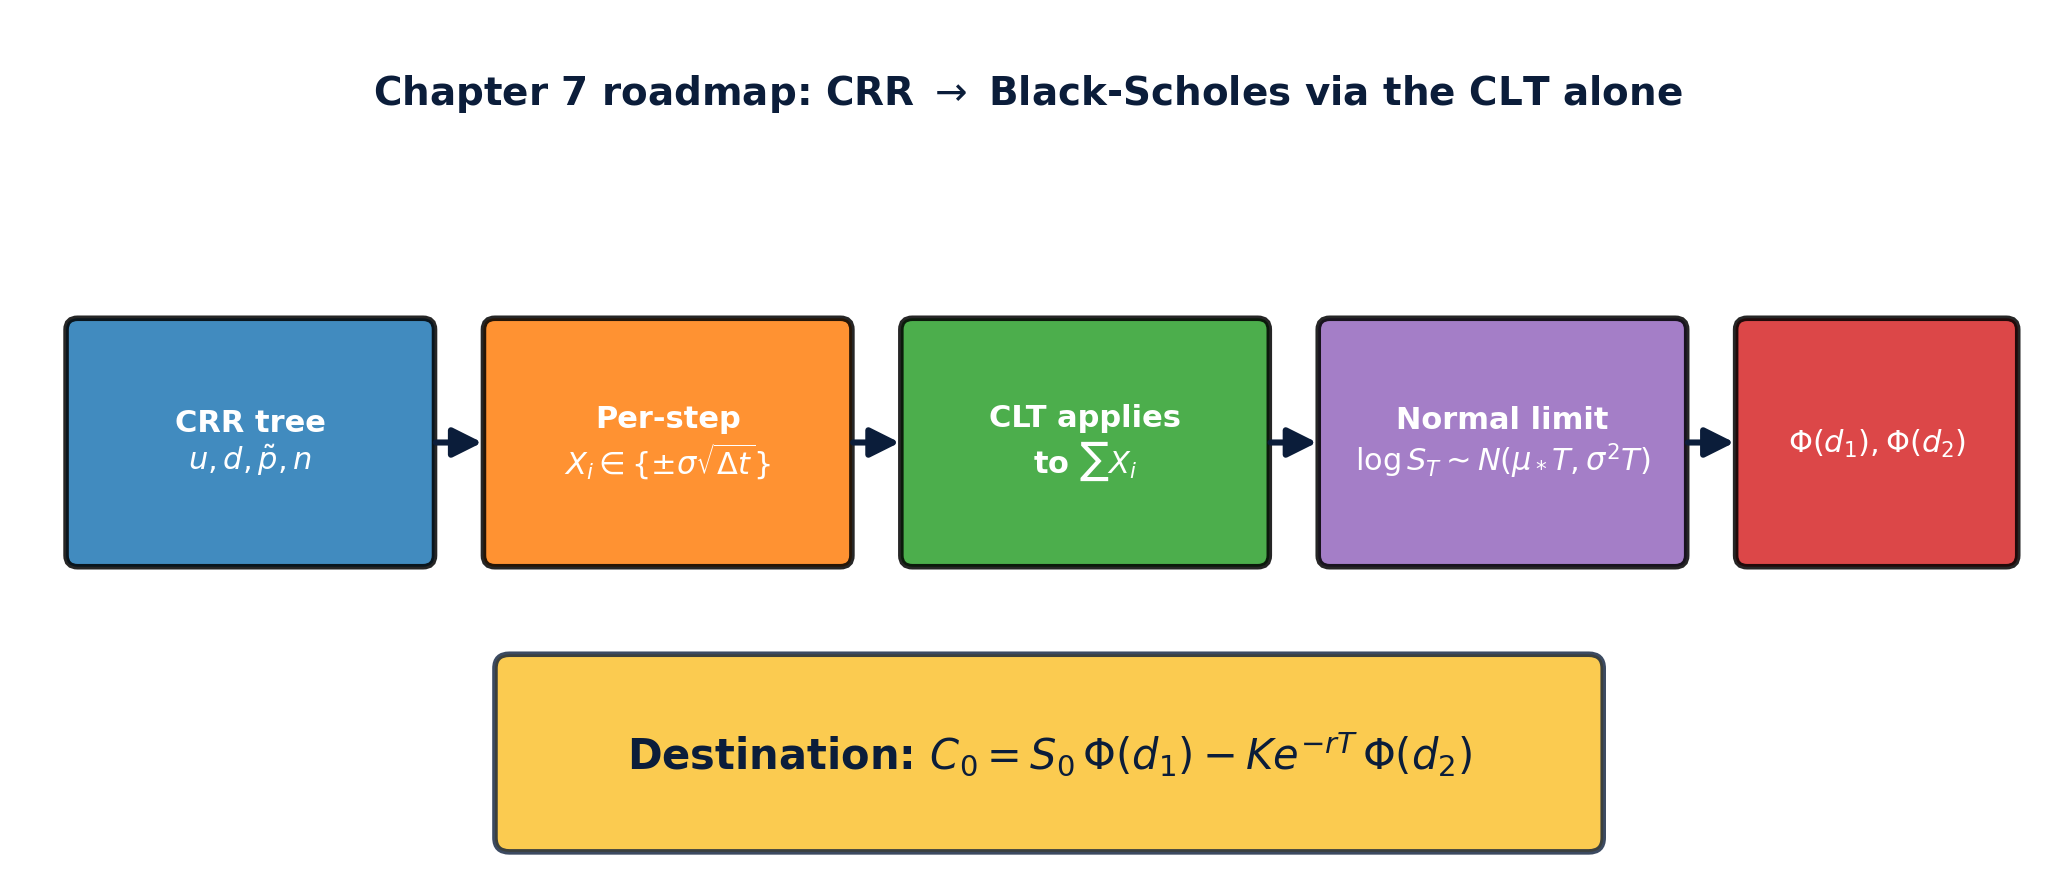
\includegraphics[keepaspectratio]{figures/ch07-roadmap.png}}
\caption{Roadmap. The CRR tree decomposes into per-step log-return
increments \(X_i\) taking values \(\pm\sigma\sqrt{\Delta t}\). By the
CLT (Ch 0 §0.10), \(\sum X_i\) becomes normal as \(n\to\infty\). The
terminal distribution of \(\log(S_T/S_0)\) is therefore
\(N(\mu_*T, \sigma^2 T)\) with \(\mu_* = r-\sigma^2/2\). From there,
\(\Phi(d_1)\) and \(\Phi(d_2)\) pop out and the BS formula is
assembled.}
\end{figure}

\subsection{7.1.2 First, just compute the
destination}\label{first-just-compute-the-destination}

Before deriving anything, let's see what the answer \emph{looks} like
for the running case and a few neighbours. That way every step of the
derivation has a number to land on.

\textbf{Example 7.1.1 (running case at maturity).} \(S_0 = K = 100\),
\(r = 0.05\), \(\sigma = 0.20\), \(T = 1\).

\[d_1 \;=\; \frac{\log(1) + (0.05 + 0.02)\cdot 1}{0.20 \cdot 1} \;=\; 0.35, \qquad d_2 \;=\; 0.35 - 0.20 \;=\; 0.15.\]

From Chapter 0's \(\Phi\)-table (or any standard-normal CDF lookup):
\(\Phi(0.35) = 0.6368\), \(\Phi(0.15) = 0.5596\). Therefore

\[C_0 \;=\; 100 \cdot 0.6368 \;-\; 100 \cdot e^{-0.05} \cdot 0.5596 \;=\; 63.68 \;-\; 53.23 \;=\; 10.4506.\]

That is the number we are spending all of Chapter 7 deriving.

\textbf{Example 7.1.2 (ATM-forward strike).} Pick
\(K = S_0 e^{rT} = 100 \cdot e^{0.05} = 105.127\). Then
\(\log(S_0/K) = -rT\) exactly cancels the \(rT\) in the numerator,
leaving

\[d_{1,2} \;=\; \pm \tfrac{1}{2}\,\sigma\sqrt T \;=\; \pm 0.10.\]

So \(\Phi(d_1) = \Phi(0.10) = 0.5398\),
\(\Phi(d_2) = \Phi(-0.10) = 0.4602\), and

\[C_0 \;=\; 100 \cdot 0.5398 \;-\; 105.127 \cdot e^{-0.05} \cdot 0.4602 \;=\; 53.98 - 46.02 \;=\; 7.9656.\]

The ATM-forward call is symmetric around zero in \(d_{1,2}\); it's the
cleanest case in BS.

\textbf{Example 7.1.3 (deep ITM).} \(K = 50\). Then
\(d_1 = (\log 2 + 0.07)/0.20 = 3.81\), \(d_2 = 3.61\), both deep in the
right tail with \(\Phi \approx 1\):

\[C_0 \;\approx\; 100 \cdot 1 \;-\; 50 \cdot e^{-0.05} \cdot 1 \;=\; 100 \;-\; 47.56 \;=\; 52.44.\]

Equivalently, \(C_0 \approx S_0 - K e^{-rT}\) --- the call collapses to
the forward.

\textbf{Example 7.1.4 (deep OTM).} \(K = 200\).
\(d_1 = (\log 0.5 + 0.07)/0.20 = -3.12\), \(d_2 = -3.32\). From Chapter
0's \(\Phi\)-table \(\Phi(-3.12) \approx 0.00090\),
\(\Phi(-3.32) \approx 0.00045\), giving
\(C_0 \approx 100 \cdot 0.00090 - 200 \cdot e^{-0.05} \cdot 0.00045 \approx 0.0904 - 0.0857 \approx 0.005\).
Almost worthless.

\textbf{Example 7.1.5 (zero-vol limit).} As \(\sigma \to 0\) with
\(S_0 = K = 100\), \(r = 0.05\):

\[d_{1,2} \;=\; \frac{0 + (0.05 \pm 0)\cdot 1}{0^+} \;\to\; +\infty,\]

so \(\Phi(d_1) = \Phi(d_2) = 1\) and
\(C_0 \to S_0 - K e^{-rT} = 100 - 95.1229 = 4.877\). With no volatility
the call's payoff is deterministic:
\((S_0 e^{rT} - K)^+ = (105.13 - 100)^+ = 5.13\), discounted to
\(4.877\). ✓

\textbf{Intuition.} The BS formula says: the call costs
\(S_0 \Phi(d_1)\), which is the present value of \emph{receiving the
stock if it ends up in the money}, minus \(K e^{-rT} \Phi(d_2)\), the
present value of \emph{paying \(K\) if it ends up in the money}. The two
\(\Phi\)'s are two different probabilities of the same event, computed
under two different measures (Chapter 3 §3.7 introduced the idea of a
measure change; we will recognise it again in §7.7).

\subsection{7.1.3 A 3-D feel for the
surface}\label{a-3-d-feel-for-the-surface}

The BS price is a smooth surface in \((S_0, T)\) for fixed
\(K, r, \sigma\):

\begin{figure}
\centering
\pandocbounded{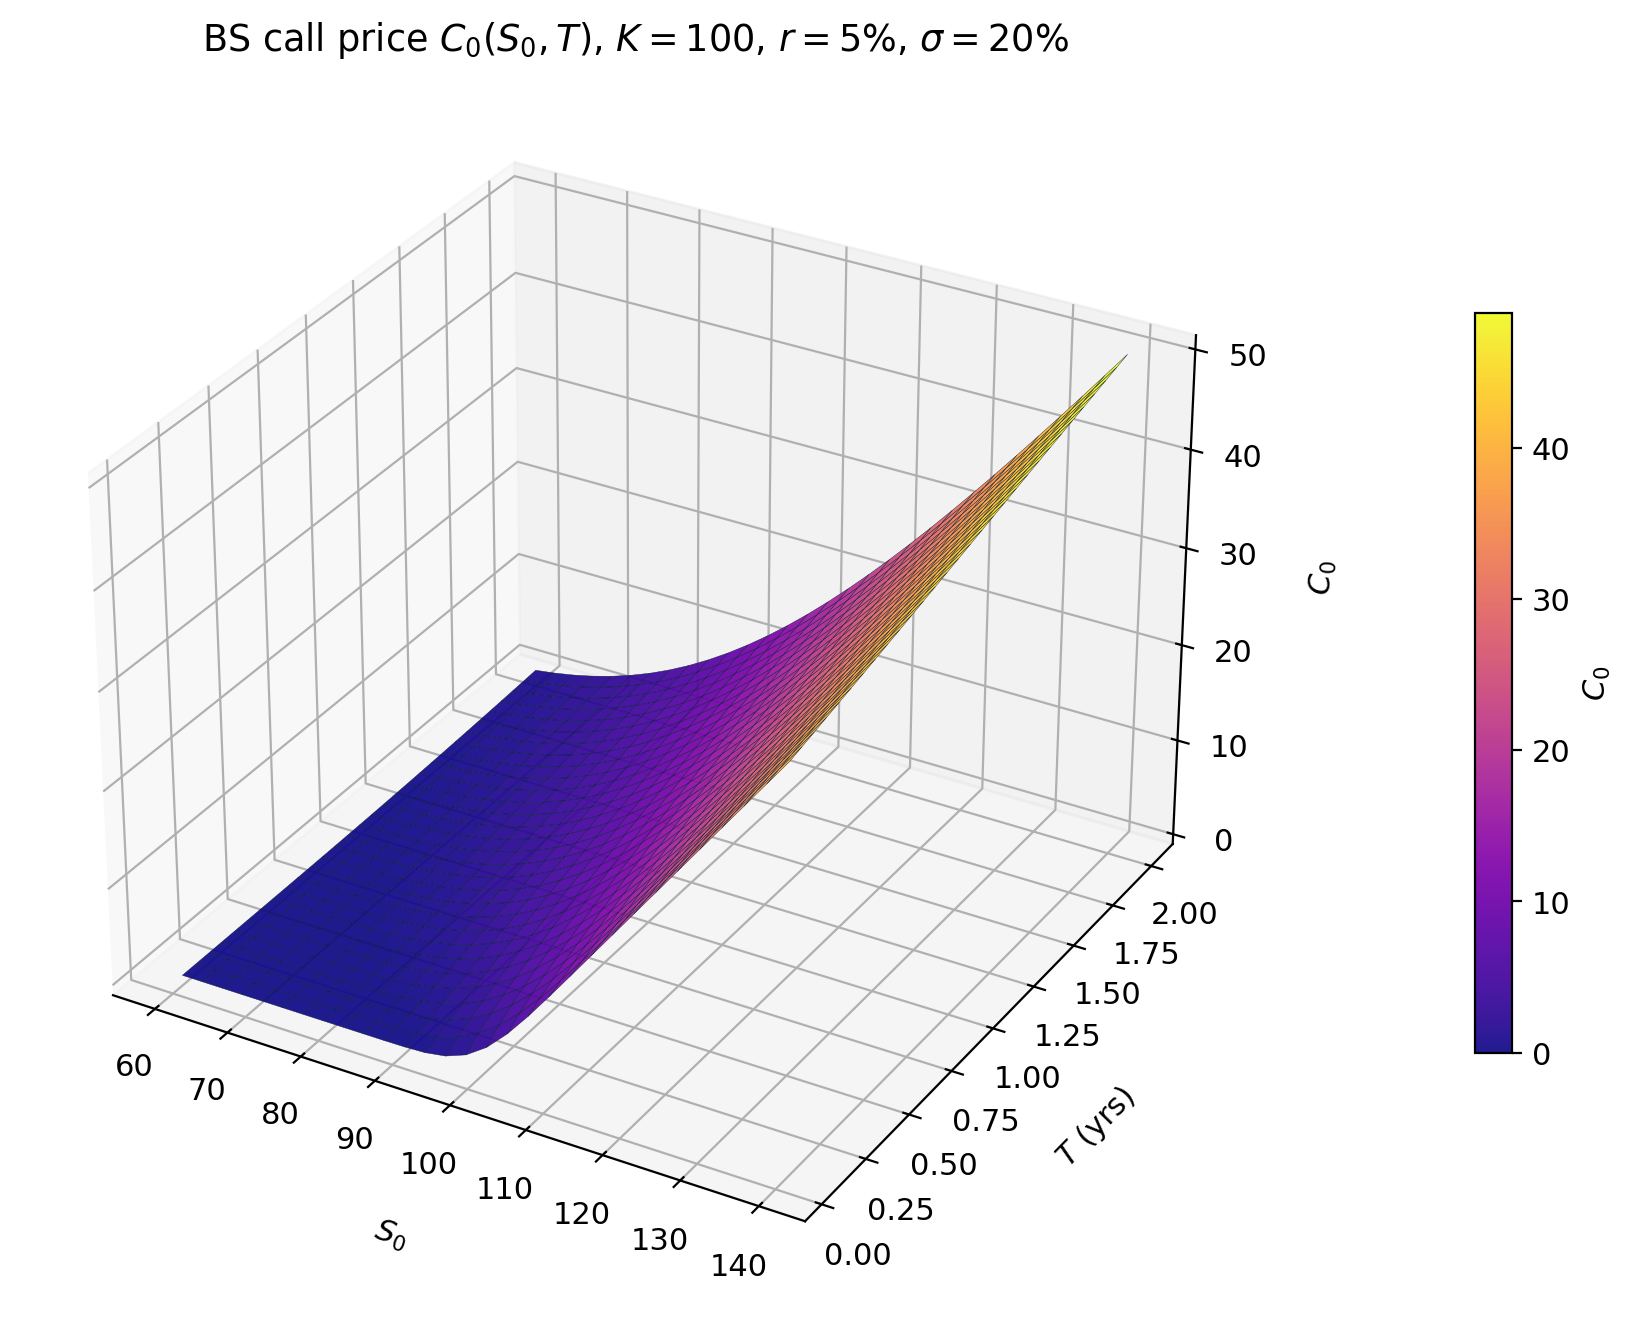
\includegraphics[keepaspectratio]{figures/ch07-C0-surface-3d.png}}
\caption{BS call price \(C_0(S_0, T)\) for \(K=100\), \(r=5\%\),
\(\sigma=20\%\). The price grows with both spot and time; it is convex
in \(S_0\) (positive gamma, §7.10) and increases with \(T\) (positive
theta-of-time-to-expiry from the perspective of the long, ignoring the
carry term). At \(T=0\) the surface is exactly the payoff kink
\((S_0-K)^+\).}
\end{figure}

\subsection{7.1.4 A grid you can read
off}\label{a-grid-you-can-read-off}

\textbf{Table 7.1.} BS call prices \(C_0\) across strike and volatility
(\(S_0=100\), \(r=5\%\), \(T=1\)).

{\def\LTcaptype{none} % do not increment counter
\begin{table}[H]
\centering
\begin{tabular}{|r|r|r|r|r|r|}
\toprule
\(\sigma \backslash K\) & \(80\) & \(90\) & \(100\) & \(110\) & \(120\) \\
\midrule



\(10\%\) & \(23.91\) & \(14.60\) & \(\phantom{0}6.81\) &
\(\phantom{0}2.04\) & \(\phantom{0}0.36\) \\
\(20\%\) & \(24.59\) & \(16.70\) & \(10.45\) & \(\phantom{0}6.04\) &
\(\phantom{0}3.25\) \\
\(30\%\) & \(26.78\) & \(19.69\) & \(13.85\) & \(\phantom{0}9.39\) &
\(\phantom{0}6.13\) \\
\(40\%\) & \(29.69\) & \(22.94\) & \(17.32\) & \(12.71\) &
\(\phantom{0}9.13\) \\
\(50\%\) & \(32.95\) & \(26.31\) & \(20.85\) & \(16.10\) & \(12.21\) \\
\bottomrule
\end{tabular}
\end{table}
}

Two patterns to remember: prices rise monotonically in \(\sigma\) (vega
\textgreater{} 0, §7.10), and the price increment per \(10\%\) extra
volatility is biggest for at-the-money strikes --- where the optionality
is most uncertain.

\begin{center}\rule{0.5\linewidth}{0.5pt}\end{center}

\section{§7.2 The CRR parametrisation}\label{the-crr-parametrisation}

\textbf{Punchline.} To make the CRR tree of Chapter 2 \emph{agree with a
continuous-time volatility} \(\sigma\), choose the up and down factors
so that \emph{each step has variance \(\sigma^2 \Delta t\) in the log
return}. The clean choice (CRR) is

\[\boxed{\;\begin{aligned}
u &= e^{\sigma\sqrt{\Delta t}}, \quad d = \tfrac{1}{u} = e^{-\sigma\sqrt{\Delta t}}, \\
r_n &= e^{r\Delta t} - 1, \\
\tilde p_n &= \frac{e^{r\Delta t} - e^{-\sigma\sqrt{\Delta t}}}{e^{\sigma\sqrt{\Delta t}} - e^{-\sigma\sqrt{\Delta t}}}.
\end{aligned}\;}\]

Here \(\Delta t = T/n\) is the per-step length. The choice \(ud = 1\)
makes the tree \emph{recombining} (Ch 2), and the choice
\(u = e^{\sigma\sqrt{\Delta t}}\) makes the variance per step
\emph{exactly} \(\sigma^2 \Delta t\) in the log-return (verified below).

\textbf{Intuition.} Each step is a coin flip on \(\log S\) moving
\(\pm \sigma\sqrt{\Delta t}\). The variance of a \(\pm a\) Bernoulli is
\(a^2\) (Chapter 0 §0.4); plug \(a = \sigma\sqrt{\Delta t}\) and you get
\(\sigma^2 \Delta t\). Variance is additive over independent steps, so
over \(n\) steps you accumulate
\(n \cdot \sigma^2 \Delta t = \sigma^2 T\). That is the target total
variance.

\subsection{7.2.1 The parameters, step by
step}\label{the-parameters-step-by-step}

\textbf{Example 7.2.1 (\(n=4\)).} \(\Delta t = 0.25\),
\(\sigma\sqrt{\Delta t} = 0.10\). Then

\[u = e^{0.10} = 1.10517, \quad d = e^{-0.10} = 0.90484, \quad r_n = e^{0.0125} - 1 = 0.012578.\]

\[\tilde p_4 \;=\; \frac{e^{0.0125} - 0.90484}{1.10517 - 0.90484} \;=\; \frac{0.10773}{0.20034} \;=\; 0.53777.\]

\textbf{Example 7.2.2 (\(n=16\)).} \(\Delta t = 1/16 = 0.0625\),
\(\sigma\sqrt{\Delta t} = 0.05\).

\[u = e^{0.05} = 1.05127, \quad d = e^{-0.05} = 0.95123, \quad r_n = e^{0.003125} - 1 = 0.003130,\]

\[\tilde p_{16} \;=\; \frac{e^{0.003125} - 0.95123}{1.05127 - 0.95123} \;=\; \frac{0.05190}{0.10004} \;=\; 0.51876.\]

Closer to \(1/2\) than \(n=4\) --- exactly what §7.3 predicts.

\textbf{Example 7.2.3 (\(n=256\)).}
\(\Delta t = 1/256 \approx 0.003906\),
\(\sigma\sqrt{\Delta t} = 0.0125\).

\[u = 1.012578, \quad d = 0.987578, \quad r_n = e^{0.0001953} - 1 = 0.0001954,\]

\[\tilde p_{256} \;=\; \frac{e^{0.0001953} - 0.987578}{1.012578 - 0.987578} \;=\; \frac{0.012617}{0.025000} \;=\; 0.50469.\]

Almost dead-centre. Hold on to that value --- §7.3 will derive it from a
Taylor expansion.

\subsection{7.2.2 No-arbitrage check}\label{no-arbitrage-check}

Chapter 2 required \(d < 1 + r_n < u\) for no-arb. For CRR:

\[d \;=\; e^{-\sigma\sqrt{\Delta t}} \;<\; e^{r\Delta t} \;<\; e^{\sigma\sqrt{\Delta t}} \;=\; u\]

holds whenever \(|r\Delta t| < \sigma\sqrt{\Delta t}\),
i.e.~\(\sigma > r\sqrt{\Delta t}\). For our running numbers,
\(r\sqrt{\Delta t} = 0.05 \cdot 1 = 0.05\) at \(n=1\) and shrinks like
\(1/\sqrt n\); the condition \(\sigma = 0.20 > 0.05\) is satisfied for
all \(n \ge 1\). So no-arb holds for the entire range we will use.

\subsection{7.2.3 Recombining check}\label{recombining-check}

\(ud = e^{\sigma\sqrt{\Delta t}} \cdot e^{-\sigma\sqrt{\Delta t}} = 1\).
So an up-then-down step lands at the same price as a down-then-up step
--- the tree recombines and has \((n+1)\) terminal nodes instead of
\(2^n\). The same observation from Ch 2.

\subsection{7.2.4 Per-step variance}\label{per-step-variance}

\textbf{Example 7.2.4 (per-step log-return variance).} Each step's log
return \(X_i\) takes values \(+\sigma\sqrt{\Delta t}\) with prob
\(\tilde p_n\) and \(-\sigma\sqrt{\Delta t}\) with prob
\(1 - \tilde p_n\). By Ch 0 §0.4:

\[\mathrm{Var}_{\tilde{\mathbb P}}(X_i) \;=\; 4\,\tilde p_n (1-\tilde p_n)\,\sigma^2 \Delta t \;\to\; \sigma^2 \Delta t,\]

because \(\tilde p_n \to 1/2\) (so \(4\tilde p_n(1-\tilde p_n) \to 1\)).
For \(n = 16\), \(4 \cdot 0.51876 \cdot 0.48124 = 0.99860\), so the
per-step variance is \(0.998 \cdot 0.0025 = 0.0024965\) --- within
\(0.14\%\) of the target.

\subsection{\texorpdfstring{7.2.5 Visualising the tree as \(n\)
grows}{7.2.5 Visualising the tree as n grows}}\label{visualising-the-tree-as-n-grows}

\begin{figure}
\centering
\pandocbounded{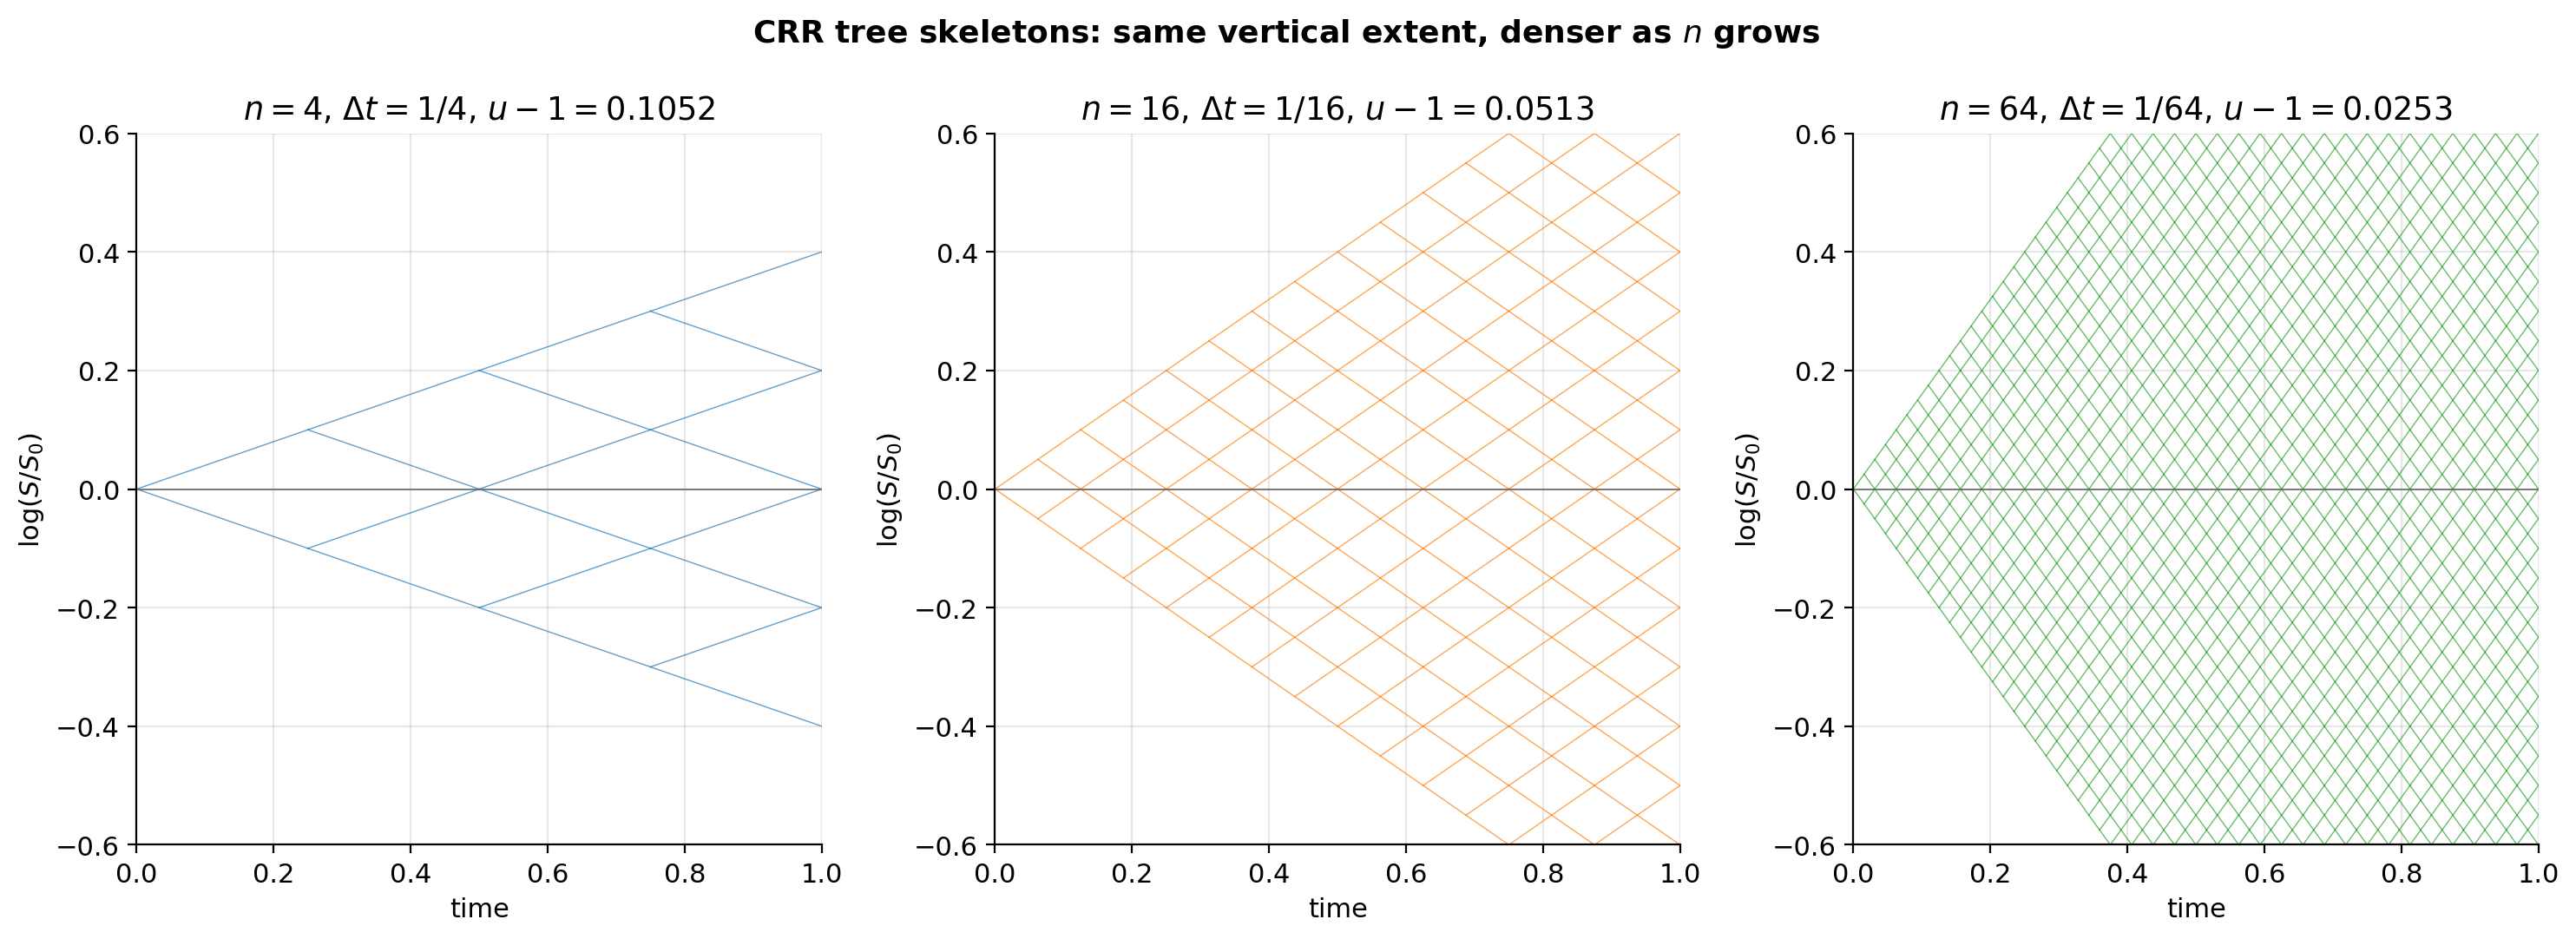
\includegraphics[keepaspectratio]{figures/ch07-tree-skeletons.png}}
\caption{CRR tree skeletons at \(n = 4, 16, 64\). All three share the
same vertical extent of \(\pm 3\sigma\sqrt T = \pm 0.60\). The branches
simply get denser as \(n\) grows; the per-step move shrinks like
\(1/\sqrt n\). This is what ``\(\Delta t \to 0\)'' looks like in
pictures.}
\end{figure}

\subsection{\texorpdfstring{7.2.6 Convergence of
\(\tilde p_n\)}{7.2.6 Convergence of \textbackslash tilde p\_n}}\label{convergence-of-tilde-p_n}

\begin{figure}
\centering
\pandocbounded{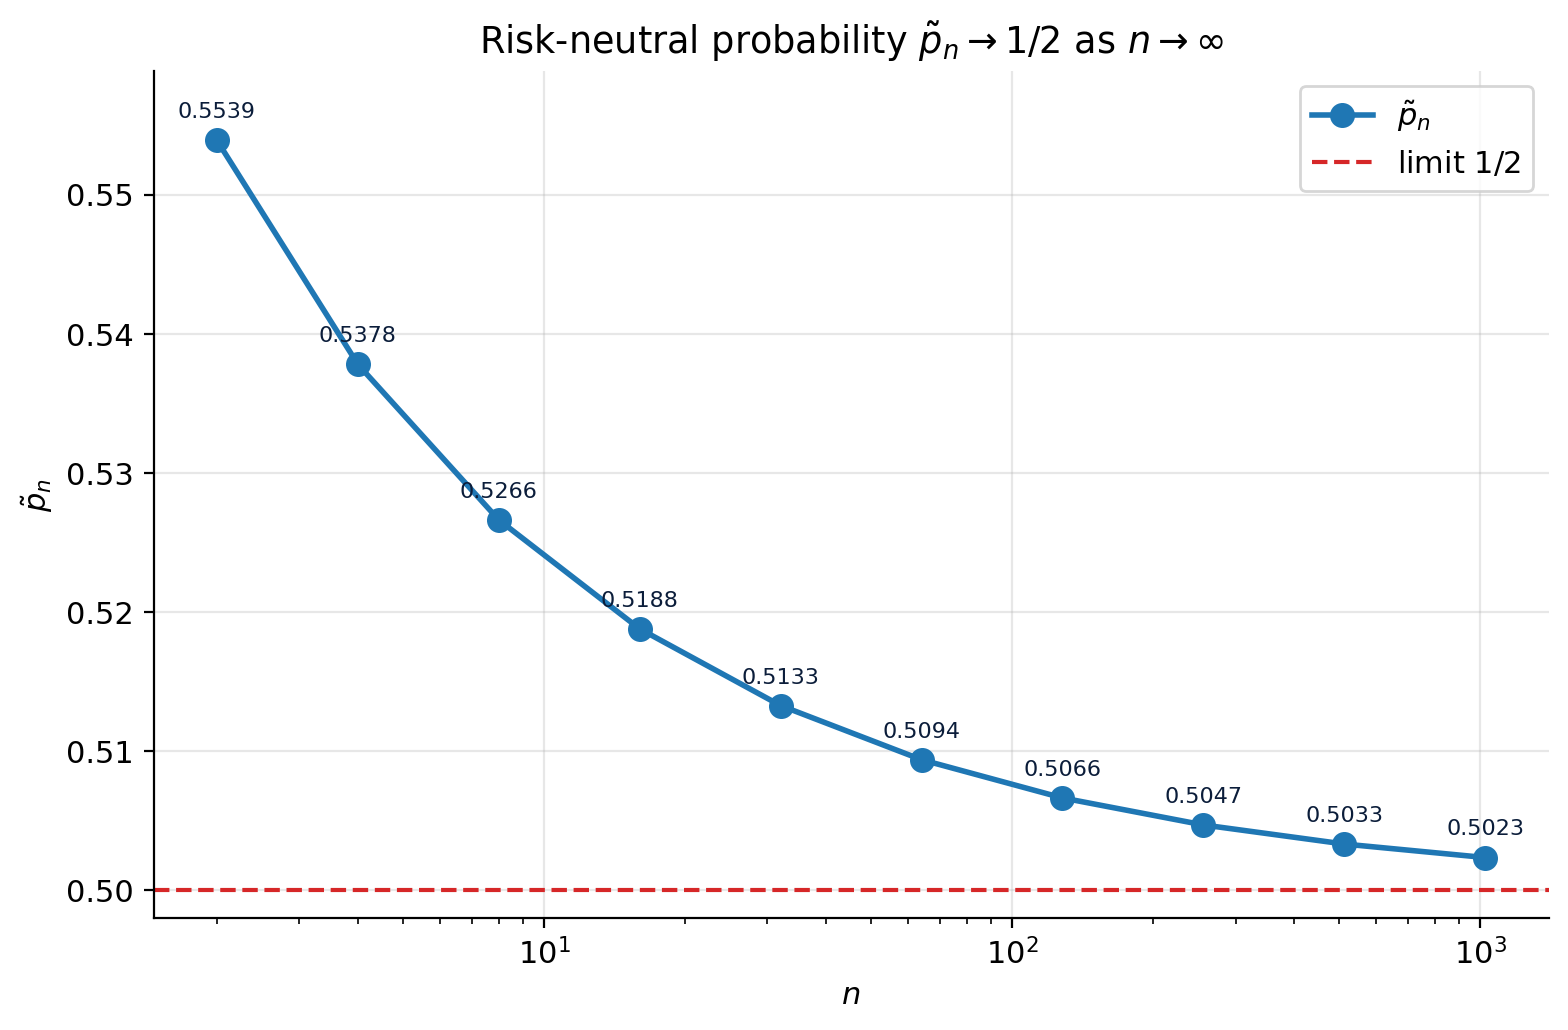
\includegraphics[keepaspectratio]{figures/ch07-tildep-vs-n.png}}
\caption{Risk-neutral probability \(\tilde p_n\) as a function of \(n\)
on a log-\(n\) scale. The sequence converges to \(1/2\) from above
(because \(r > 0\)); the speed is \(O(1/\sqrt n)\), derived in §7.3.}
\end{figure}

\subsection{7.2.7 The big parameter
table}\label{the-big-parameter-table}

\textbf{Table 7.2.} CRR parameters across \(n\) for the running case
(\(\sigma = 0.20\), \(r = 0.05\), \(T = 1\)).

{\def\LTcaptype{none} % do not increment counter
\begin{table}[H]
\centering
\begin{tabular}{|r|r|r|r|r|r|}
\toprule
\(n\) & \(\Delta t\) & \(u_n\) & \(d_n\) & \(r_n\) & \(\tilde p_n\) \\
\midrule



\(\phantom{000}2\) & \(0.500000\) & \(1.1519\) & \(0.8681\) &
\(0.0253150\) & \(0.55397\) \\
\(\phantom{000}4\) & \(0.250000\) & \(1.1052\) & \(0.9048\) &
\(0.0125780\) & \(0.53777\) \\
\(\phantom{000}8\) & \(0.125000\) & \(1.0733\) & \(0.9317\) &
\(0.0062700\) & \(0.52681\) \\
\(\phantom{00}16\) & \(0.062500\) & \(1.0513\) & \(0.9512\) &
\(0.0031300\) & \(0.51876\) \\
\(\phantom{00}32\) & \(0.031250\) & \(1.0359\) & \(0.9653\) &
\(0.0015630\) & \(0.51322\) \\
\(\phantom{00}64\) & \(0.015625\) & \(1.0253\) & \(0.9753\) &
\(0.0007810\) & \(0.50934\) \\
\(\phantom{0}128\) & \(0.007813\) & \(1.0179\) & \(0.9824\) &
\(0.0003910\) & \(0.50661\) \\
\(\phantom{0}256\) & \(0.003906\) & \(1.0126\) & \(0.9876\) &
\(0.0001950\) & \(0.50469\) \\
\(\phantom{0}512\) & \(0.001953\) & \(1.0089\) & \(0.9912\) &
\(0.0000977\) & \(0.50331\) \\
\(1024\) & \(0.000977\) & \(1.0063\) & \(0.9938\) & \(0.0000488\) &
\(0.50234\) \\
\bottomrule
\end{tabular}
\end{table}
}

\begin{center}\rule{0.5\linewidth}{0.5pt}\end{center}

\section{\texorpdfstring{§7.3 Sanity check on
\(\tilde p_n\)}{§7.3 Sanity check on \textbackslash tilde p\_n}}\label{sanity-check-on-tilde-p_n}

\textbf{Punchline.} As \(n\to\infty\), \(\tilde p_n \to 1/2\), but the
\emph{deviation} from \(1/2\) encodes the entire risk-neutral drift
\(\mu_* = r - \sigma^2/2\):

\[\boxed{\; \tilde p_n \;\approx\; \frac{1}{2} \;+\; \frac{\mu_*\sqrt{\Delta t}}{2\sigma} \;}, \qquad \mu_* \;=\; r - \frac{\sigma^2}{2}.\]

\textbf{Intuition.} A symmetric \(\pm \sigma\sqrt{\Delta t}\) walk with
\(\tilde p_n = 1/2\) exactly would drift by zero. To get the
risk-neutral expectation \(\tilde{\mathbb E}[S_T] = S_0 e^{rT}\), the up
probability must be tilted slightly above \(1/2\). The \(-\sigma^2/2\)
correction in \(\mu_*\) comes from the convexity of \(\log\) --- the
same convexity correction we met in Ch 0 §0.1 (``up 50\% then down 50\%
is not breakeven''). It is \emph{not} a calculus artefact; it is purely
the difference between \(\tilde{\mathbb E}[\log S]\) and
\(\log \tilde{\mathbb E}[S]\).

\subsection{7.3.1 Where the approximation comes
from}\label{where-the-approximation-comes-from}

Expand \(e^{x}\) around \(x = 0\) as far as second order (Ch 0 §0.2
stated it as a fact, no calculus required):

\[e^x \;\approx\; 1 + x + \tfrac{x^2}{2}.\]

Apply to \(u\), \(d\), and \(e^{r\Delta t}\) in \(\tilde p_n\):

\[u = 1 + \sigma\sqrt{\Delta t} + \tfrac{1}{2}\sigma^2 \Delta t, \quad d = 1 - \sigma\sqrt{\Delta t} + \tfrac{1}{2}\sigma^2 \Delta t, \quad e^{r\Delta t} = 1 + r\Delta t.\]

Numerator:
\(e^{r\Delta t} - d \approx r\Delta t + \sigma\sqrt{\Delta t} - \tfrac{1}{2}\sigma^2 \Delta t = \sigma\sqrt{\Delta t} + (r - \tfrac{1}{2}\sigma^2)\Delta t = \sigma\sqrt{\Delta t} + \mu_*\Delta t\).

Denominator: \(u - d \approx 2\sigma\sqrt{\Delta t}\).

Ratio:

\[\tilde p_n \;\approx\; \frac{\sigma\sqrt{\Delta t} + \mu_* \Delta t}{2\sigma\sqrt{\Delta t}} \;=\; \frac{1}{2} \;+\; \frac{\mu_* \sqrt{\Delta t}}{2\sigma}.\]

The Taylor expansion is the \emph{only} analytic tool we ever use in
this chapter --- and we use it just to identify which terms in
\(\Delta t\) matter.

\subsection{7.3.2 Test the approximation}\label{test-the-approximation}

\textbf{Example 7.3.1.} \(n = 16\), \(\Delta t = 1/16\). With
\(\mu_* = 0.05 - 0.02 = 0.03\), \(\sigma = 0.20\):

\[\tilde p_{16}^{approx} \;=\; \frac{1}{2} \;+\; \frac{0.03 \cdot 0.25}{2 \cdot 0.20} \;=\; 0.5 + 0.01875 \;=\; 0.51875.\]

Exact (from Table 7.2): \(0.51876\). Error: \(10^{-5}\). The Taylor
approximation is essentially exact at \(n = 16\).

\textbf{Example 7.3.2.} \(n = 256\), \(\Delta t = 1/256\).

\[\tilde p_{256}^{approx} \;=\; 0.5 + \frac{0.03 \cdot 0.0625}{0.40} \;=\; 0.5 + 0.0046875 \;=\; 0.504688.\]

Exact: \(0.50469\). Error: \(2 \cdot 10^{-6}\).

\textbf{Example 7.3.3 (\(2\tilde p_n - 1\) is what's interesting).}
Rewrite:

\[2\tilde p_n - 1 \;\approx\; \frac{\mu_* \sqrt{\Delta t}}{\sigma}.\]

This is the \emph{net drift} in coin-flip language:
\(\tilde{\mathbb P}(\text{up}) - \tilde{\mathbb P}(\text{down})\). For
\(n = 16\): \((2 \cdot 0.51876) - 1 = 0.03752\) and
\(\mu_*\sqrt{\Delta t}/\sigma = 0.03 \cdot 0.25 / 0.20 = 0.0375\). ✓

\textbf{Example 7.3.4 (\(\tilde p_n (1 - \tilde p_n) \to 1/4\)).}
Per-step variance scales as
\(4\tilde p_n(1-\tilde p_n)\sigma^2\Delta t\). Since
\(\tilde p_n \to 1/2\), \(\tilde p_n(1-\tilde p_n) \to 1/4\) and
\(4\tilde p_n(1-\tilde p_n) \to 1\). The variance fits its target
\(\sigma^2\Delta t\) asymptotically, which is exactly what §7.4 needs.

\subsection{7.3.3 Visualising the
approximation}\label{visualising-the-approximation}

\begin{figure}
\centering
\pandocbounded{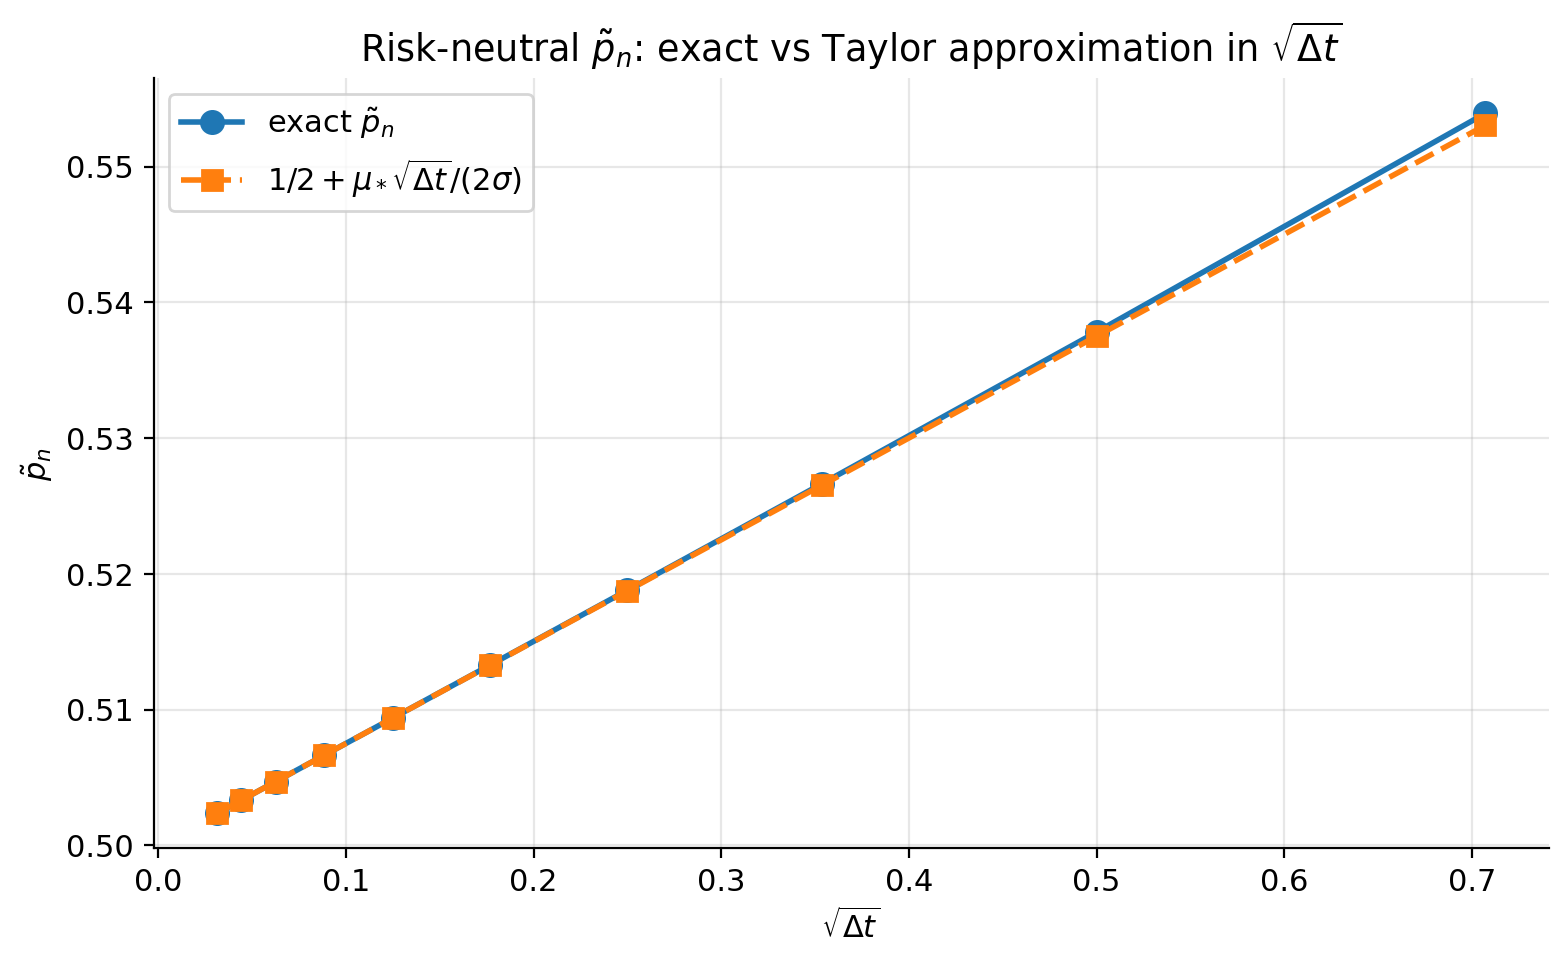
\includegraphics[keepaspectratio]{figures/ch07-tildep-approx.png}}
\caption{Exact \(\tilde p_n\) (blue circles) versus the Taylor
approximation \(1/2 + \mu_*\sqrt{\Delta t}/(2\sigma)\) (orange squares)
on the horizontal axis \(\sqrt{\Delta t}\). The two are visually
indistinguishable; the approximation is a \emph{linear} function of
\(\sqrt{\Delta t}\), which is the cleanest way to plot what is going
on.}
\end{figure}

\subsection{\texorpdfstring{7.3.4 Table of \(\tilde p_n\)
errors}{7.3.4 Table of \textbackslash tilde p\_n errors}}\label{table-of-tilde-p_n-errors}

\textbf{Table 7.3.} \(\tilde p_n\): exact, Taylor approximation, and
error.

\emph{Approximation:}
\(\tilde p_n^{\text{approx}} = 1/2 + \mu_*\sqrt{\Delta t}/(2\sigma)\).

{\def\LTcaptype{none} % do not increment counter
\begin{table}[H]
\centering
\begin{tabular}{|r|r|r|r|}
\toprule
\(n\) & exact \(\tilde p_n\) & approx & error \(\times 10^{-5}\) \\
\midrule



\(\phantom{000}4\) & \(0.53777\) & \(0.53750\) & \(\phantom{-0}26.8\) \\
\(\phantom{000}8\) & \(0.52681\) & \(0.52652\) & \(\phantom{-0}29.0\) \\
\(\phantom{00}16\) & \(0.51876\) & \(0.51875\) & \(\phantom{-00}1.4\) \\
\(\phantom{00}32\) & \(0.51322\) & \(0.51326\) & \(\phantom{-0}-4.2\) \\
\(\phantom{00}64\) & \(0.50934\) & \(0.50938\) & \(\phantom{-0}-3.5\) \\
\(\phantom{0}128\) & \(0.50661\) & \(0.50663\) & \(\phantom{-0}-2.5\) \\
\(\phantom{0}256\) & \(0.50469\) & \(0.50469\) & \(\phantom{-0}-0.2\) \\
\(\phantom{0}512\) & \(0.50331\) & \(0.50331\) & \(\phantom{-00}0.0\) \\
\(1024\) & \(0.50234\) & \(0.50234\) & \(\phantom{-00}0.0\) \\
\bottomrule
\end{tabular}
\end{table}
}

For everything we do later, treating \(\tilde p_n\) as
\(1/2 + \mu_*\sqrt{\Delta t}/(2\sigma)\) would be enough.

\begin{center}\rule{0.5\linewidth}{0.5pt}\end{center}

\section{§7.4 The log-return per step}\label{the-log-return-per-step}

\textbf{Punchline.} Each CRR step contributes mean \(\mu_*\Delta t\) and
variance \(\sigma^2\Delta t\) to the log-return. Over \(n\) steps the
means sum to \(\mu_* T\) and the variances sum to \(\sigma^2 T\). The
CLT (Ch 0 §0.10) then says the \emph{standardised} sum is asymptotically
\(N(0,1)\), i.e.

\[\boxed{\; \log\!\frac{S_T}{S_0} \;=\; \sum_{i=1}^n X_i \;\;\xrightarrow{d}\;\; N(\mu_* T, \,\sigma^2 T). \;}\]

\textbf{Intuition.} Variances of independent random variables add. So do
means. CRR's clever per-step variance of \(\sigma^2\Delta t\) makes the
\emph{total} variance \(\sigma^2 T\) no matter how many steps we slice
\(T\) into. And the bookkeeping in \(\tilde p_n\) (§7.3) ensures the
total mean is \(\mu_* T\). Once you have a sum of \(n\) i.i.d. things
with finite variance, the CLT applies --- full stop.

\subsection{7.4.1 Per-step mean and
variance}\label{per-step-mean-and-variance}

Each step
\(X_i \in \{+\sigma\sqrt{\Delta t},\, -\sigma\sqrt{\Delta t}\}\) with
probabilities \(\tilde p_n, 1-\tilde p_n\). From the moments of a
\(\pm a\) Bernoulli (Ch 0 §0.4):

\[\tilde{\mathbb E}[X_i] \;=\; (2\tilde p_n - 1)\,\sigma\sqrt{\Delta t}, \qquad \mathrm{Var}_{\tilde{\mathbb P}}(X_i) \;=\; 4\tilde p_n(1-\tilde p_n)\,\sigma^2 \Delta t.\]

Substitute the §7.3 approximation
\(2\tilde p_n - 1 \approx \mu_*\sqrt{\Delta t}/\sigma\):

\[\tilde{\mathbb E}[X_i] \;\approx\; \mu_* \Delta t, \qquad \mathrm{Var}_{\tilde{\mathbb P}}(X_i) \;\to\; \sigma^2 \Delta t.\]

\subsection{7.4.2 Running numbers, step by
step}\label{running-numbers-step-by-step}

\textbf{Example 7.4.1.} \(\sigma = 0.20\), \(\Delta t = 1/16\). Then
\(X_i \in \{+0.05, -0.05\}\), and

\[\tilde{\mathbb E}[X_i] \;=\; (2 \cdot 0.51876 - 1) \cdot 0.05 \;=\; 0.03752 \cdot 0.05 \;=\; 0.001876.\]

Predicted: \(\mu_*\Delta t = 0.03 \cdot 0.0625 = 0.001875\). ✓
(Three-figure match.)

\textbf{Example 7.4.2 (sum the means).} Over \(n=16\) steps, the total
expected log-return is
\(16 \cdot 0.001876 = 0.03001 \approx 0.03 = \mu_* T\). ✓

\textbf{Example 7.4.3 (sum the variances).} Per-step variance is
\(4 \cdot 0.51876 \cdot 0.48124 \cdot 0.0025 = 0.002496\). Times \(16\)
gives \(0.03994 \approx 0.04 = \sigma^2 T\). ✓

\textbf{Example 7.4.4 (skewness shrinks).} The clean statement: the
\emph{skewness of the sum} of \(n\) i.i.d. \(\pm a\) Bernoullis falls as
\(1/\sqrt n\). For the running case, the skewness of \(\sum X_i\) at
\(n = 16\) is about \(-0.094\); at \(n = 256\) it is \(-0.024\). The
distribution becomes increasingly symmetric, as the CLT predicts.

\textbf{Example 7.4.5 (kurtosis correction).} Excess kurtosis of the sum
also falls as \(1/n\): from about \(-0.001\) at \(n=16\) to
\(-6\times 10^{-5}\) at \(n=256\). The normal limit has zero excess
kurtosis; we are converging to it.

\textbf{Example 7.4.6 (sanity check:
\(\tilde{\mathbb E}[S_T] = S_0 e^{rT}\)).} By construction of
\(\tilde p_n\),
\(\tilde{\mathbb E}[S_{i+1} | S_i] = S_i \cdot e^{r\Delta t}\).
Iterating, \(\tilde{\mathbb E}[S_T] = S_0 e^{rT}\) exactly, at
\emph{every} \(n\). The convergence of \emph{log returns} to a normal
does not change the constraint on the mean of \(S_T\) itself --- it just
tells us \emph{how} \(\log S_T\) is distributed.

\subsection{7.4.3 Histogram evidence}\label{histogram-evidence}

\begin{figure}
\centering
\pandocbounded{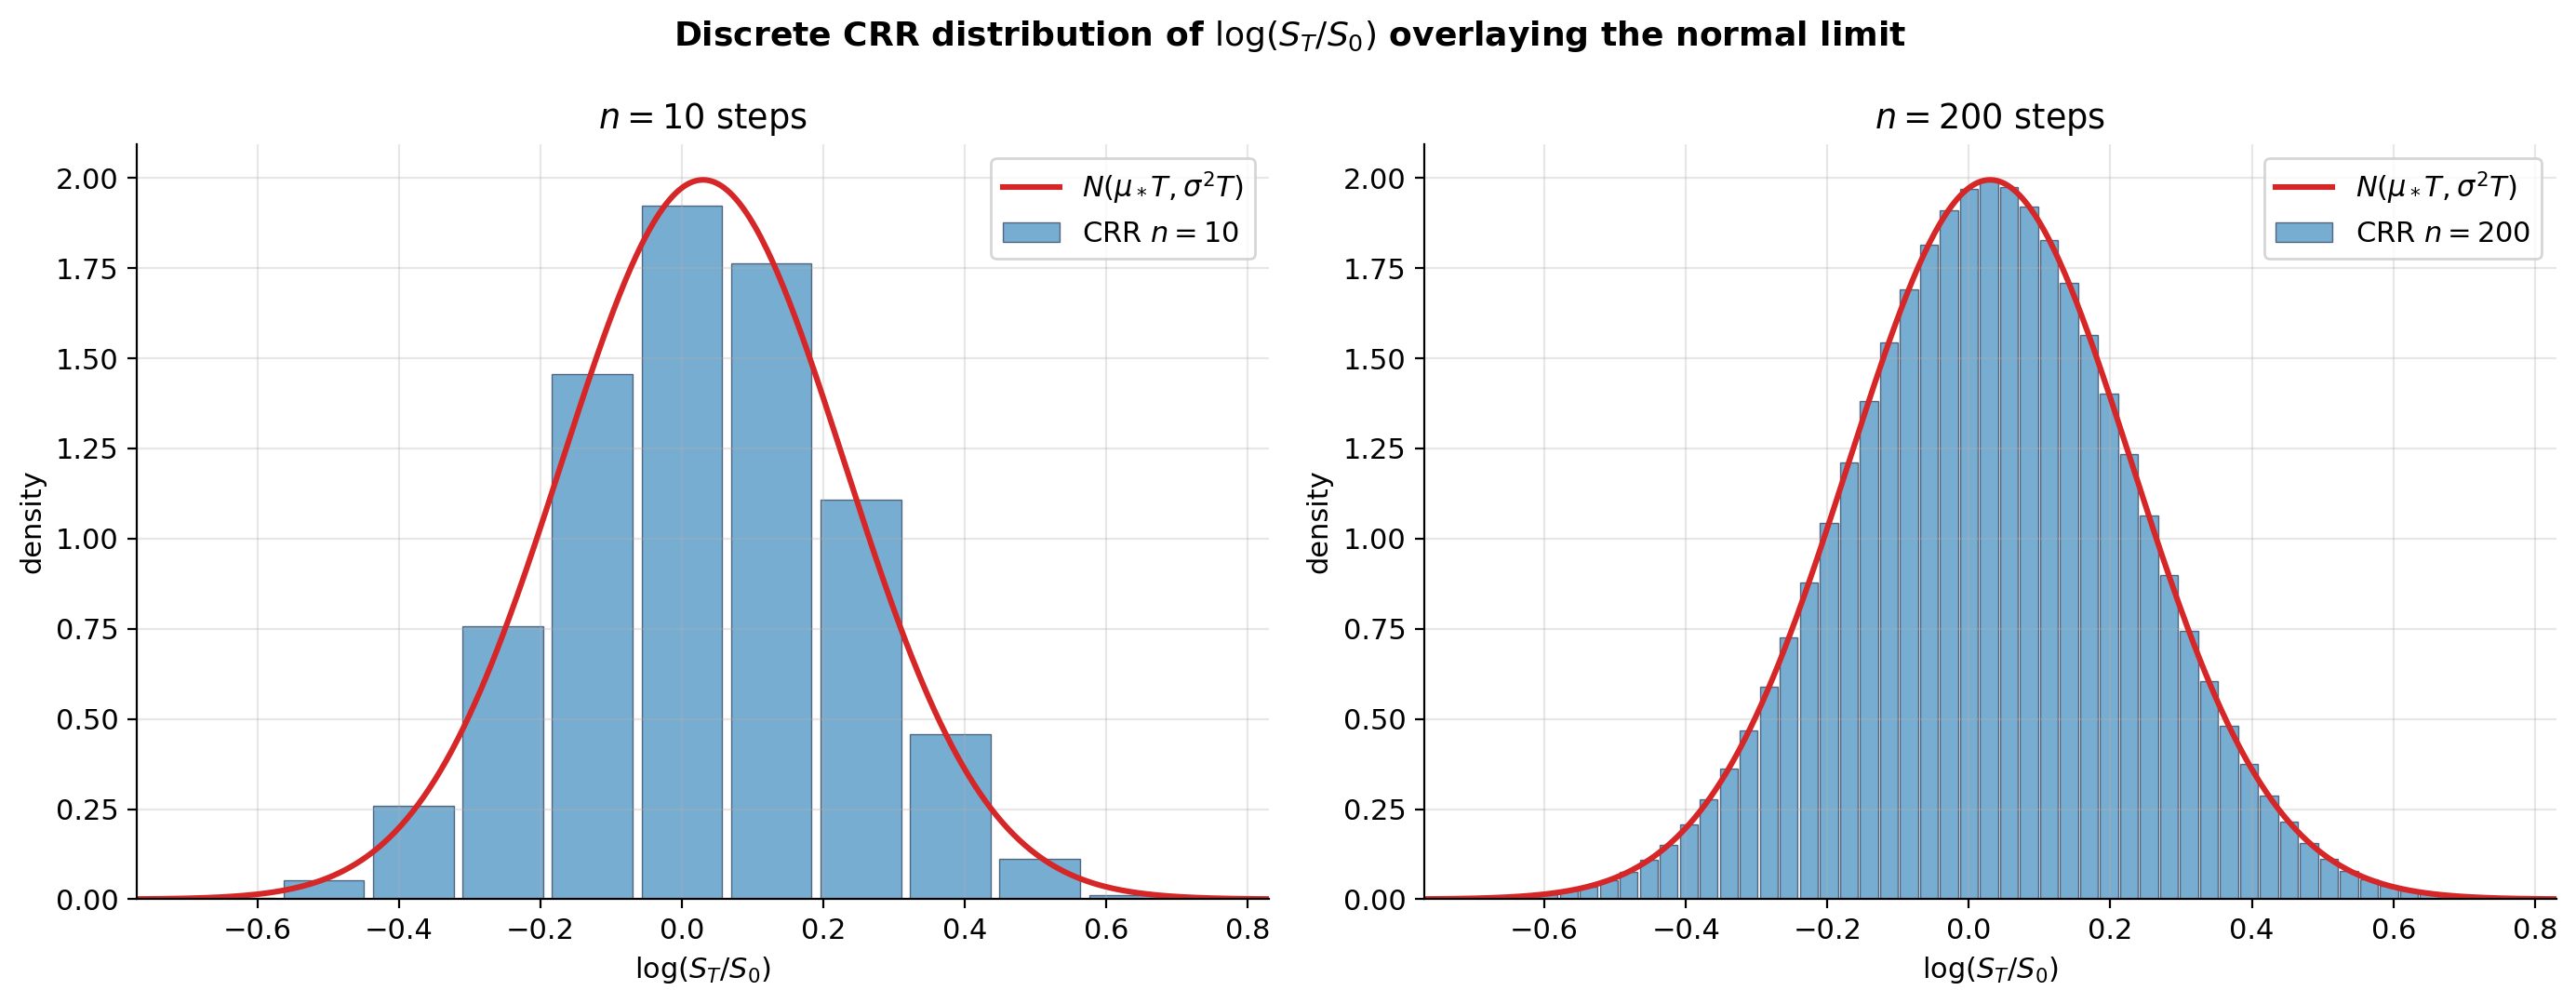
\includegraphics[keepaspectratio]{figures/ch07-logS-histograms.png}}
\caption{Two CRR histograms of the terminal log-return
\(\log(S_T/S_0)\). Left: \(n=10\) (coarse, lumpy). Right: \(n=200\)
(already indistinguishable from the smooth red normal curve
\(N(\mu_* T, \sigma^2 T)\)). The CRR pmf is converted to a density by
dividing each lump's probability by the bin width
\(2\sigma\sqrt{\Delta t}\).}
\end{figure}

\subsection{7.4.4 A 3-D view of
convergence}\label{a-3-d-view-of-convergence}

\begin{figure}
\centering
\pandocbounded{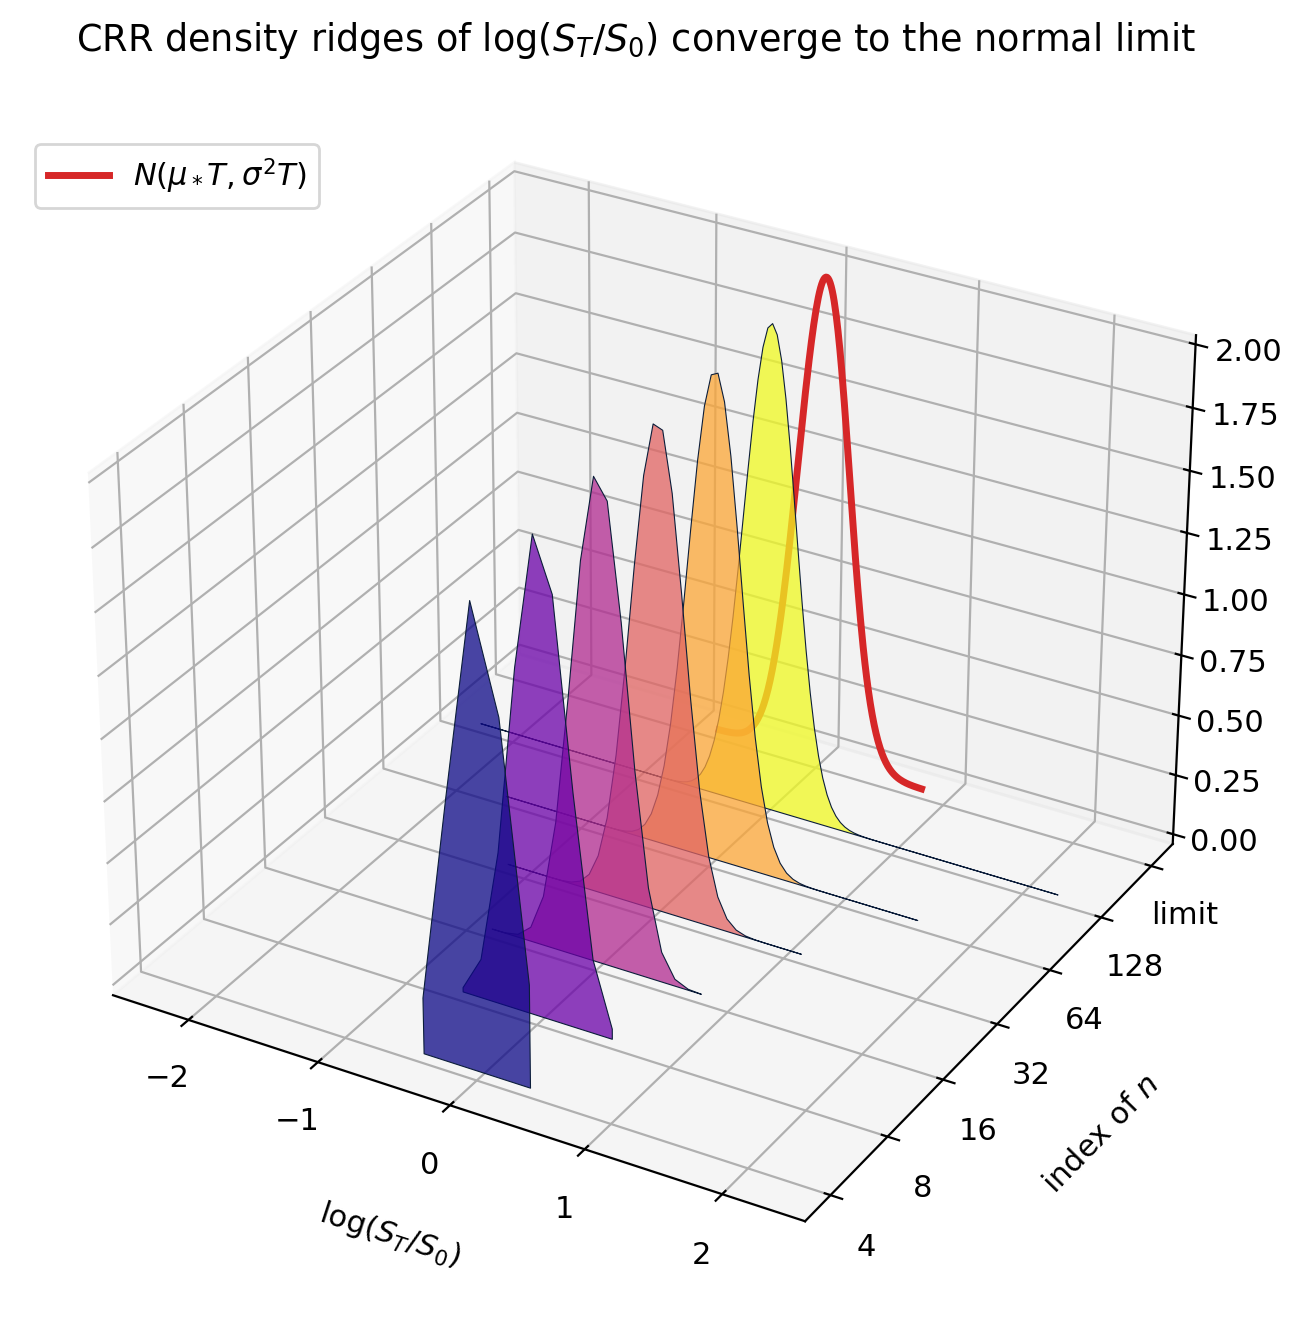
\includegraphics[keepaspectratio]{figures/ch07-density-ridge-3d.png}}
\caption{Density of \(\log(S_T/S_0)\) as \(n\) grows from \(4\) to
\(128\). Each ridge is a CRR distribution; the red curve at the back is
the normal limit. Visual confirmation of the CLT in action for our
specific sequence.}
\end{figure}

\subsection{7.4.5 Convergence table}\label{convergence-table}

\textbf{Table 7.4.} Mean and variance of the CRR log-return sum, by
\(n\). Targets: \(\mu_* T = 0.03\), \(\sigma^2 T = 0.04\).

\emph{Columns:} mean \(= \sum_i \tilde{\mathbb E}[X_i]\); variance
\(= \sum_i \mathrm{Var}_{\tilde{\mathbb P}}(X_i)\).

{\def\LTcaptype{none} % do not increment counter
\begin{table}[H]
\centering
\begin{tabular}{|r|r|r|}
\toprule
\(n\) & mean & variance \\
\midrule



\(\phantom{000}4\) & \(0.030193\) & \(0.039429\) \\
\(\phantom{000}8\) & \(0.030096\) & \(0.039720\) \\
\(\phantom{00}16\) & \(0.030048\) & \(0.039861\) \\
\(\phantom{00}32\) & \(0.030024\) & \(0.039931\) \\
\(\phantom{00}64\) & \(0.030012\) & \(0.039965\) \\
\(\phantom{0}128\) & \(0.030006\) & \(0.039983\) \\
\(\phantom{0}256\) & \(0.030003\) & \(0.039991\) \\
\(\phantom{0}512\) & \(0.030002\) & \(0.039996\) \\
target & \(0.030000\) & \(0.040000\) \\
\bottomrule
\end{tabular}
\end{table}
}

\begin{center}\rule{0.5\linewidth}{0.5pt}\end{center}

\section{\texorpdfstring{§7.5 Apply the CLT --- \emph{the
moment}}{§7.5 Apply the CLT --- the moment}}\label{apply-the-clt-the-moment}

\textbf{Punchline.} Combine §7.3 and §7.4 with the CLT statement of Ch 0
§0.10:

\[\boxed{\;\; \log\!\frac{S_T}{S_0} \;\;\xrightarrow{d}\;\; N\!\bigl(\,(r - \tfrac{1}{2}\sigma^2)\,T,\; \sigma^2 T\,\bigr) \;\;}\]

Equivalently, with \(Z \sim N(0,1)\),

\[S_T \;\stackrel{d}{=}\; S_0 \,\exp\!\Bigl(\mu_* T \;+\; \sigma\sqrt T\, Z\Bigr), \qquad \mu_* = r - \tfrac{1}{2}\sigma^2.\]

That's the whole game in one line. Everything else in this chapter is
plug-and-grind.

\textbf{Intuition.} This is \emph{lognormal} dynamics for \(S_T\):
\(S_T\) is the exponential of a normal. The mean of \(\log S_T\) is
\(\log S_0 + \mu_* T\); the variance is \(\sigma^2 T\). The mean of
\(S_T\) itself is \(S_0 e^{rT}\) (by Ch 0 §0.9's identity
\(\mathbb E[e^Y] = e^{m + s^2/2}\) for \(Y\sim N(m,s^2)\), with
\(m = \log S_0 + \mu_* T\), \(s^2 = \sigma^2 T\): gives
\(S_0 e^{\mu_* T + \sigma^2 T/2} = S_0 e^{rT}\) ✓).

\subsection{7.5.1 The running example,
distributionally}\label{the-running-example-distributionally}

\textbf{Example 7.5.1 (the lognormal distribution of \(S_T\)).} With
running numbers,
\(\log S_T \sim N(\log 100 + 0.03,\, 0.04) = N(4.6352, 0.04)\). Standard
deviation of \(\log S_T\) is \(\sqrt{0.04} = 0.20 = \sigma\sqrt T\). The
mean of \(S_T\) itself is
\(e^{4.6352 + 0.02} = e^{4.6552} = 105.127 = 100 e^{0.05}\). ✓

\textbf{Example 7.5.2 (probability the stock exceeds \(110\)).} Using
the normal limit:

\[\begin{aligned}
\tilde{\mathbb P}(S_T > 110) &= \tilde{\mathbb P}\bigl(\log S_T > \log 110\bigr) \\
&= \tilde{\mathbb P}\!\left(\frac{\log(S_T/S_0) - \mu_* T}{\sigma\sqrt T} > \frac{\log 1.10 - 0.03}{0.20}\right).
\end{aligned}\]

The RHS upper bound is \(z = (0.09531 - 0.03)/0.20 = 0.3266\), so
\(\tilde{\mathbb P}(S_T > 110) = 1 - \Phi(0.3266) = 0.3720\).

\textbf{Example 7.5.3 (CRR vs limit).} Direct CRR computation at
\(n = 100\) gives \(\tilde{\mathbb P}(S_T > 110) = 0.3735\) (using the
lattice). Discrepancy: \(0.0015\) --- the same \(1/\sqrt n\) rate as
everywhere else.

\textbf{Example 7.5.4 (median vs mean).} Median of \(S_T\) is at the
median of \(\log S_T\): \(e^{4.6352} = 100 \cdot e^{0.03} = 103.045\).
Mean is \(100\cdot e^{0.05} = 105.127\). The mean is \emph{bigger} than
the median --- a generic feature of lognormals (right-skewed). The
difference is the \emph{Jensen gap}; it equals
\(S_0(e^{rT} - e^{\mu_* T}) = S_0 e^{\mu_* T}(e^{\sigma^2 T/2} - 1) \approx 2.08\),
of which the small-\(\sigma\) approximation gives
\(S_0 e^{\mu_* T} \cdot \sigma^2 T/2 = 103.04 \cdot 0.02 \approx 2.06\).
✓

\textbf{Example 7.5.5 (95\% confidence interval for \(S_T\)).}
\(\log S_T = 4.6352 \pm 1.96 \cdot 0.20\), so
\(\log S_T \in [4.2432, 5.0272]\), i.e.~\(S_T \in [69.69, 152.55]\). A
\(30\%\) to \(52\%\) swing in either direction over one year, at
\(20\%\) vol.

\subsection{7.5.2 Visual confirmation in four
panels}\label{visual-confirmation-in-four-panels}

\begin{figure}
\centering
\pandocbounded{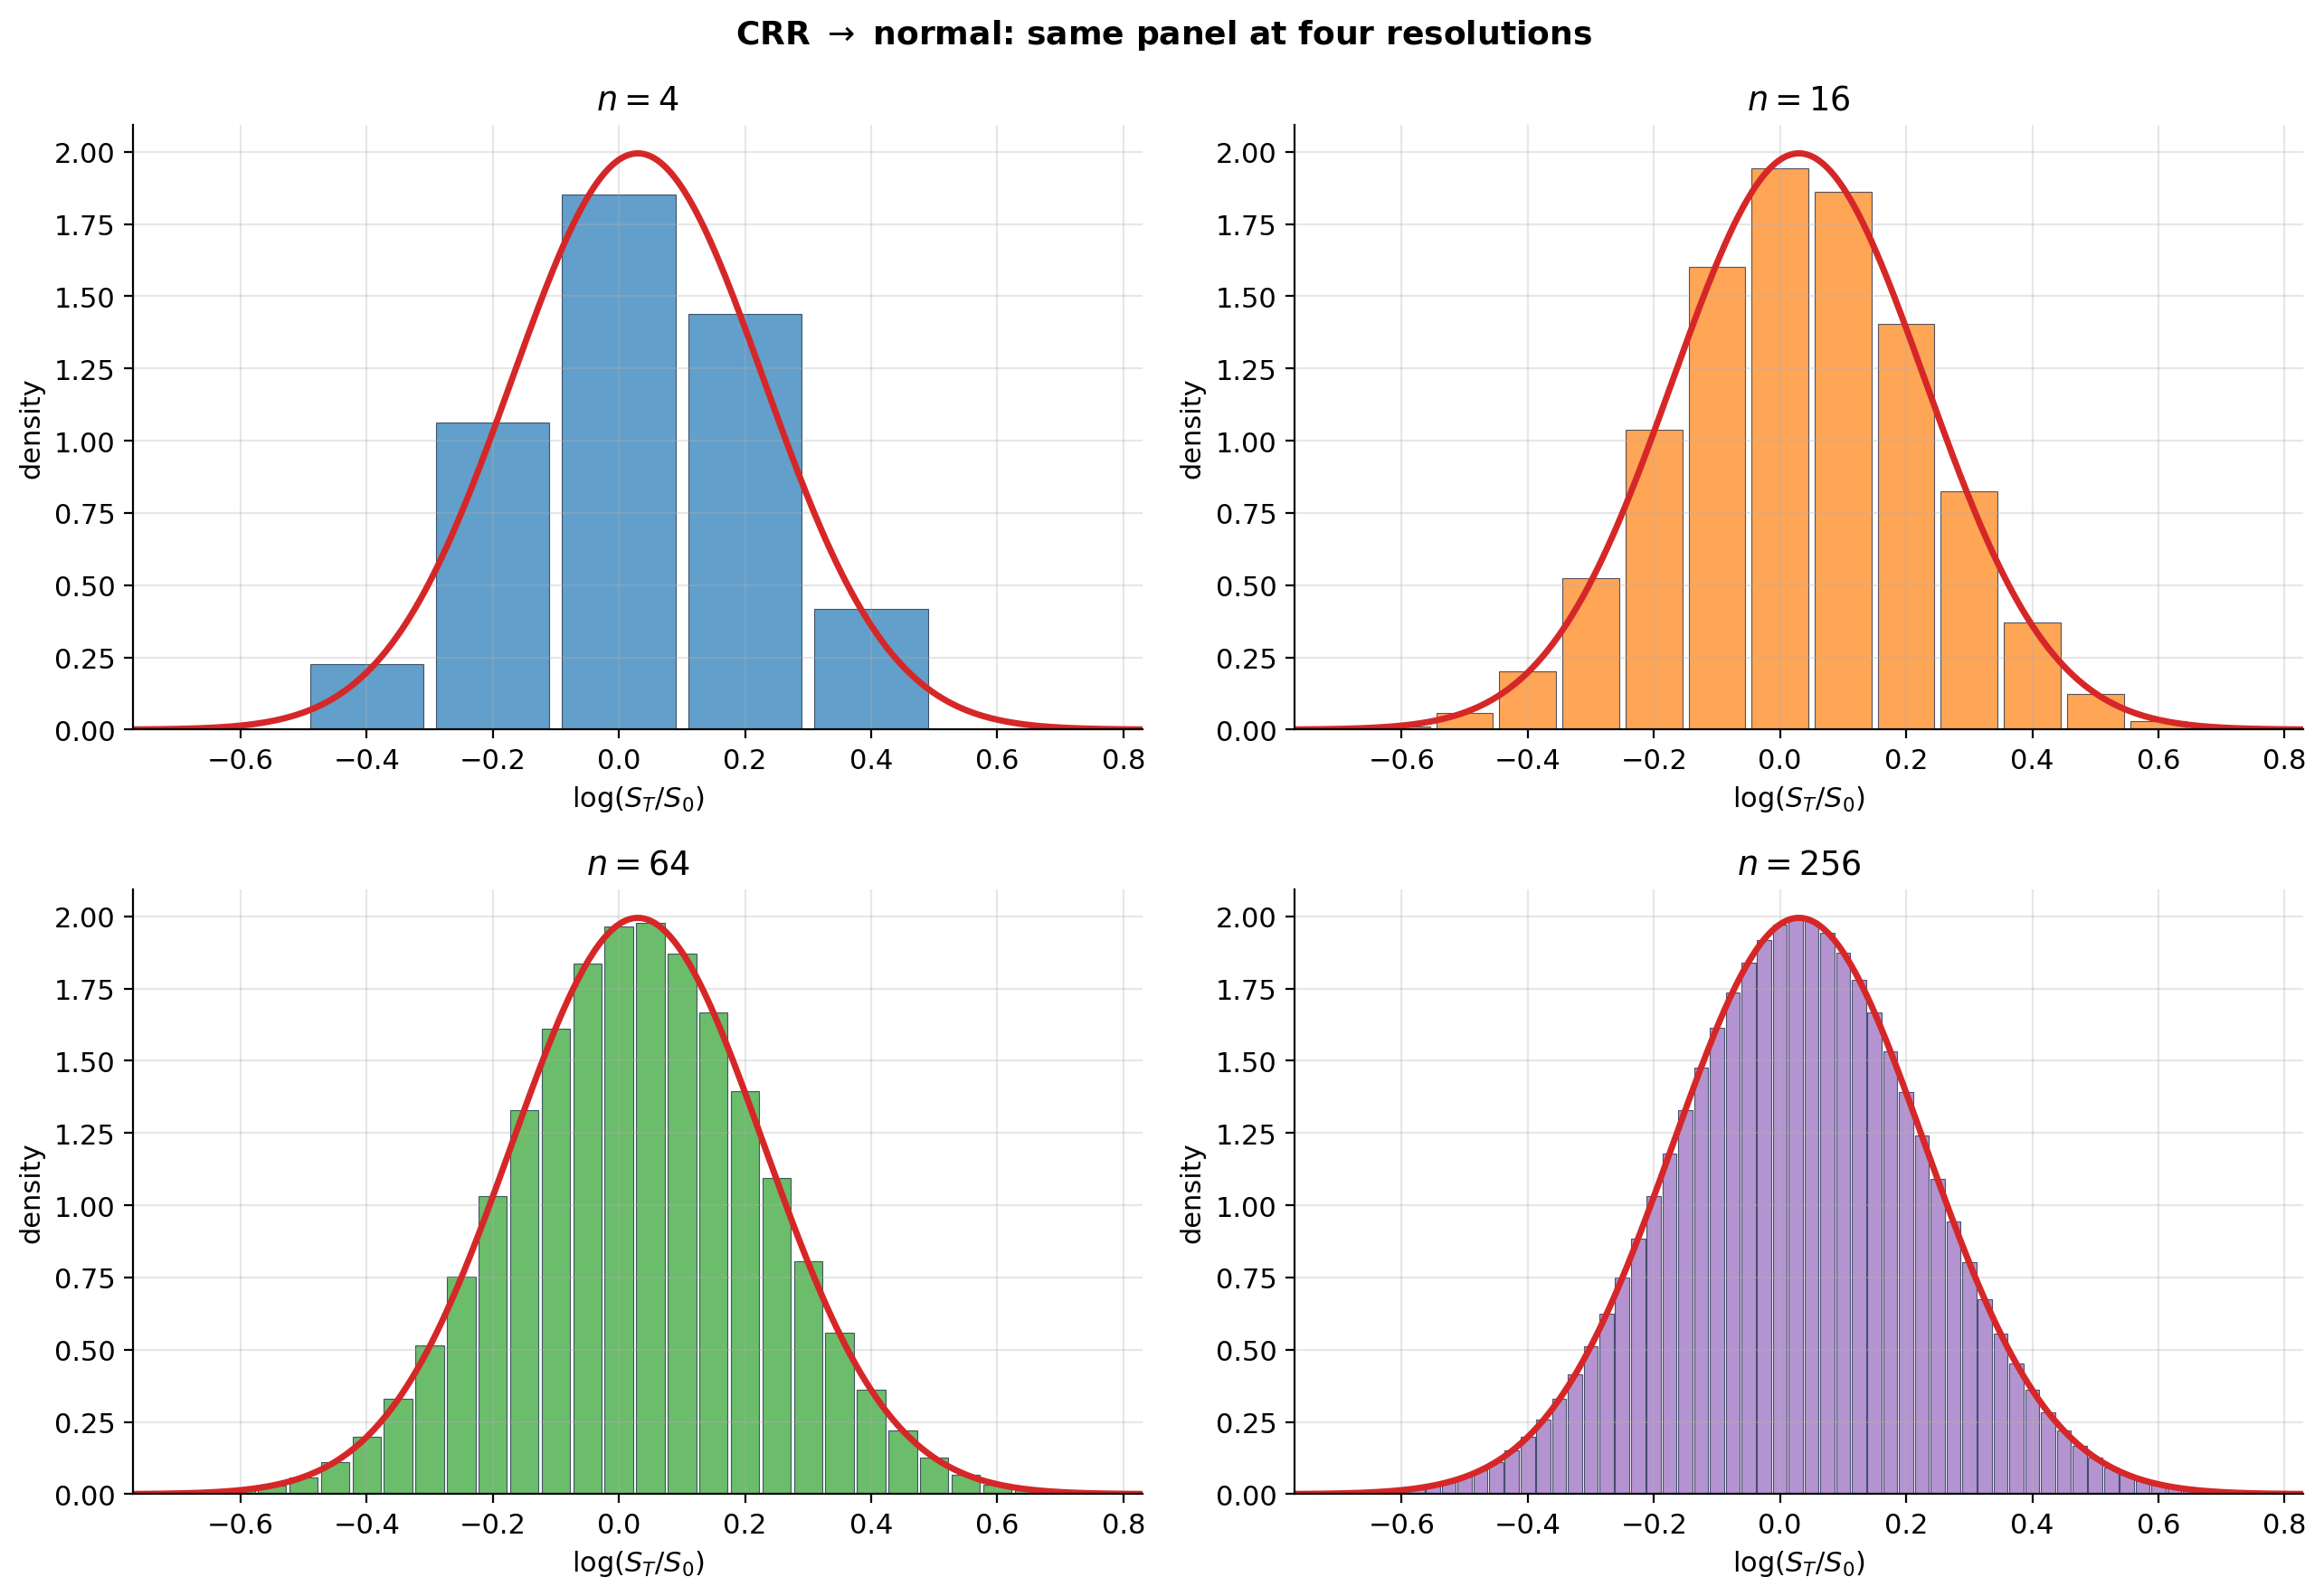
\includegraphics[keepaspectratio]{figures/ch07-binom-vs-normal-4panel.png}}
\caption{CRR pmf converted to a density, overlaid on the limiting normal
density \(N(\mu_* T, \sigma^2 T)\). At \(n=4\) the pmf is four chunky
bars; by \(n=256\) it is visually indistinguishable from the normal.
This is the CLT in pictures.}
\end{figure}

\subsection{7.5.3 Q-Q plot}\label{q-q-plot}

\begin{figure}
\centering
\pandocbounded{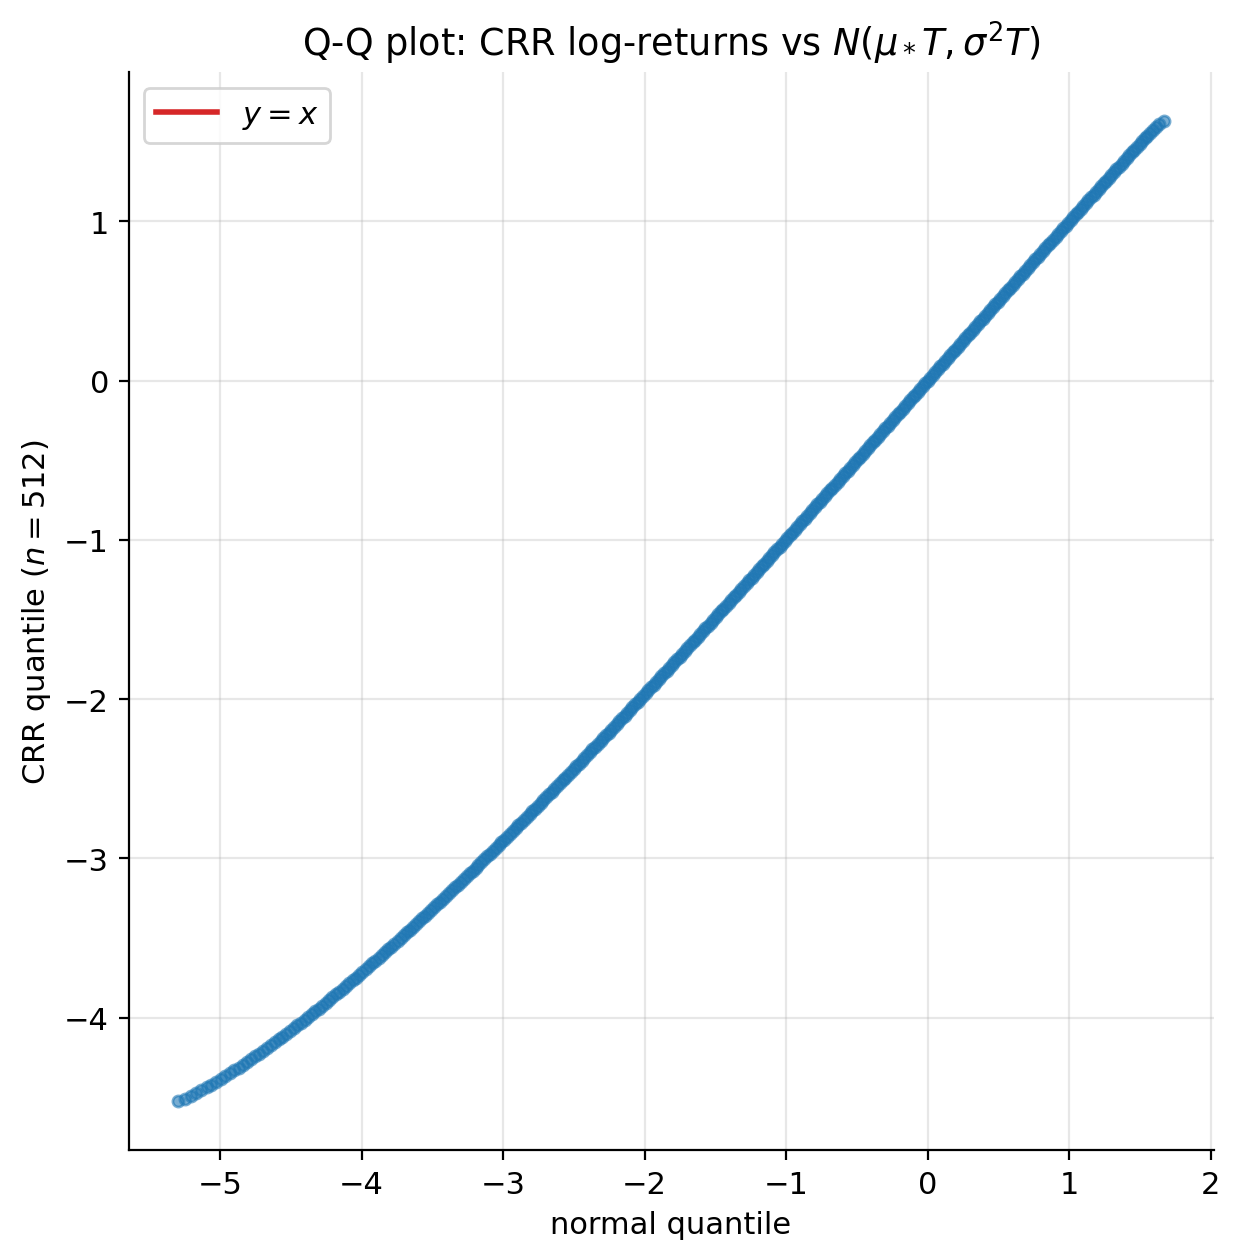
\includegraphics[keepaspectratio]{figures/ch07-qq-plot.png}}
\caption{Quantile-quantile plot of CRR log-returns at \(n = 512\)
against the normal limit. Points fall on the \(y = x\) line to within
plotting precision. (Q-Q plots magnify any tail mismatch; here there
isn't any.)}
\end{figure}

\subsection{7.5.4 Threshold-probability
table}\label{threshold-probability-table}

\textbf{Table 7.5.} \(\tilde{\mathbb P}(S_T > K)\) for the running
parameters: CRR at \(n=256\) vs the lognormal limit.

{\def\LTcaptype{none} % do not increment counter
\begin{table}[H]
\centering
\begin{tabular}{|r|r|r|r|}
\toprule
\(K\) & CRR \(n=256\) & normal limit & error \\
\midrule



\(\phantom{0}80\) & \(0.91428\) & \(0.91463\) &
\(\phantom{-}0.00035\) \\
\(\phantom{0}90\) & \(0.78115\) & \(0.78060\) & \(-0.00055\) \\
\(100\) & \(0.55927\) & \(0.55962\) & \(\phantom{-}0.00035\) \\
\(110\) & \(0.37428\) & \(0.37197\) & \(-0.00231\) \\
\(120\) & \(0.21030\) & \(0.20813\) & \(-0.00217\) \\
\(130\) & \(0.10577\) & \(0.10312\) & \(-0.00265\) \\
\(140\) & \(0.04691\) & \(0.04561\) & \(-0.00130\) \\
\bottomrule
\end{tabular}
\end{table}
}

\begin{center}\rule{0.5\linewidth}{0.5pt}\end{center}

\section{\texorpdfstring{§7.6 The CRR sum becomes
\(\Phi(d_2)\)}{§7.6 The CRR sum becomes \textbackslash Phi(d\_2)}}\label{the-crr-sum-becomes-phid_2}

\textbf{Punchline.} The ``discounted risk-neutral probability of
exercise'' --- the simpler of the two terms in BS --- converges by the
CLT to \(e^{-rT}\Phi(d_2)\):

\[\boxed{\; e^{-rT} \, \tilde{\mathbb P}(S_T \ge K) \;\to\; e^{-rT}\,\Phi(d_2) \;}, \qquad d_2 \;=\; \frac{\log(S_0/K) + (r - \tfrac{1}{2}\sigma^2) T}{\sigma\sqrt T}.\]

\textbf{Intuition.} \(\tilde{\mathbb P}(S_T \ge K)\) is a probability
under the risk-neutral measure that, by §7.5, becomes a normal-tail
probability. Standardise the normal and the bound at \(K\) becomes
\(-d_2\). Look up \(\Phi\) in the table --- done.

\subsection{7.6.1 Three lines of algebra}\label{three-lines-of-algebra}

Starting from the CLT result
\(\log(S_T/S_0) \sim N(\mu_* T, \sigma^2 T)\):

\textbf{Step 1.}
\(\{S_T \ge K\} \iff \{\log(S_T/S_0) \ge \log(K/S_0)\}\).

\textbf{Step 2.} Standardise: with
\(Z = (\log(S_T/S_0) - \mu_* T)/(\sigma\sqrt T)\),

\[\log(S_T/S_0) \ge \log(K/S_0) \;\iff\; Z \;\ge\; \frac{\log(K/S_0) - \mu_* T}{\sigma\sqrt T} \;=\; -d_2.\]

\textbf{Step 3.}
\(\tilde{\mathbb P}(Z \ge -d_2) = 1 - \Phi(-d_2) = \Phi(d_2)\) (symmetry
of the normal CDF).

Done.

\subsection{7.6.2 Plug the running case}\label{plug-the-running-case}

\textbf{Example 7.6.1.} \(S_0 = K = 100\), \(r = 0.05\),
\(\sigma = 0.20\), \(T = 1\):

\[d_2 \;=\; \frac{0 + 0.03}{0.20} \;=\; 0.15, \qquad \Phi(d_2) \;=\; 0.55962.\]

\textbf{Example 7.6.2 (CRR check at \(n = 256\)).} From Table 7.5,
\(\tilde{\mathbb P}(S_T \ge 100) = 0.55927\) at \(n = 256\). Limit:
\(0.55962\). Error: \(0.00035\).

\textbf{Example 7.6.3 (discounted form).}
\(e^{-rT} \Phi(d_2) = e^{-0.05} \cdot 0.55962 = 0.9512 \cdot 0.55962 = 0.53233\).
Multiply by \(K = 100\) to get the second term of BS:
\(100 \cdot 0.53233 = 53.233\).

\textbf{Example 7.6.4 (deep OTM).} \(K = 150\):
\(d_2 = (\log(100/150) + 0.03)/0.20 = (-0.40546 + 0.03)/0.20 = -1.877\).
\(\Phi(-1.877) \approx 0.0303\). So
\(\tilde{\mathbb P}(S_T \ge 150) \approx 3\%\).

\textbf{Example 7.6.5 (ATM-forward).} \(K = S_0 e^{rT} = 105.127\): by
Example 7.1.2, \(d_2 = -\tfrac{1}{2}\sigma\sqrt T = -0.10\).
\(\Phi(-0.10) = 0.46017\).

\textbf{Example 7.6.6 (limit as \(T \to 0\)).}
\(d_2 \to \mathrm{sgn}(\log(S_0/K))\cdot \infty\). If \(S_0 > K\),
\(\Phi(d_2) \to 1\); if \(S_0 < K\), \(\Phi(d_2) \to 0\). So at
\(T = 0\), \(\tilde{\mathbb P}(S_T \ge K) = \mathbf 1_{S_0 \ge K}\).
Sensible: there is no time for anything to happen.

\subsection{7.6.3 Visual confirmation}\label{visual-confirmation}

\begin{figure}
\centering
\pandocbounded{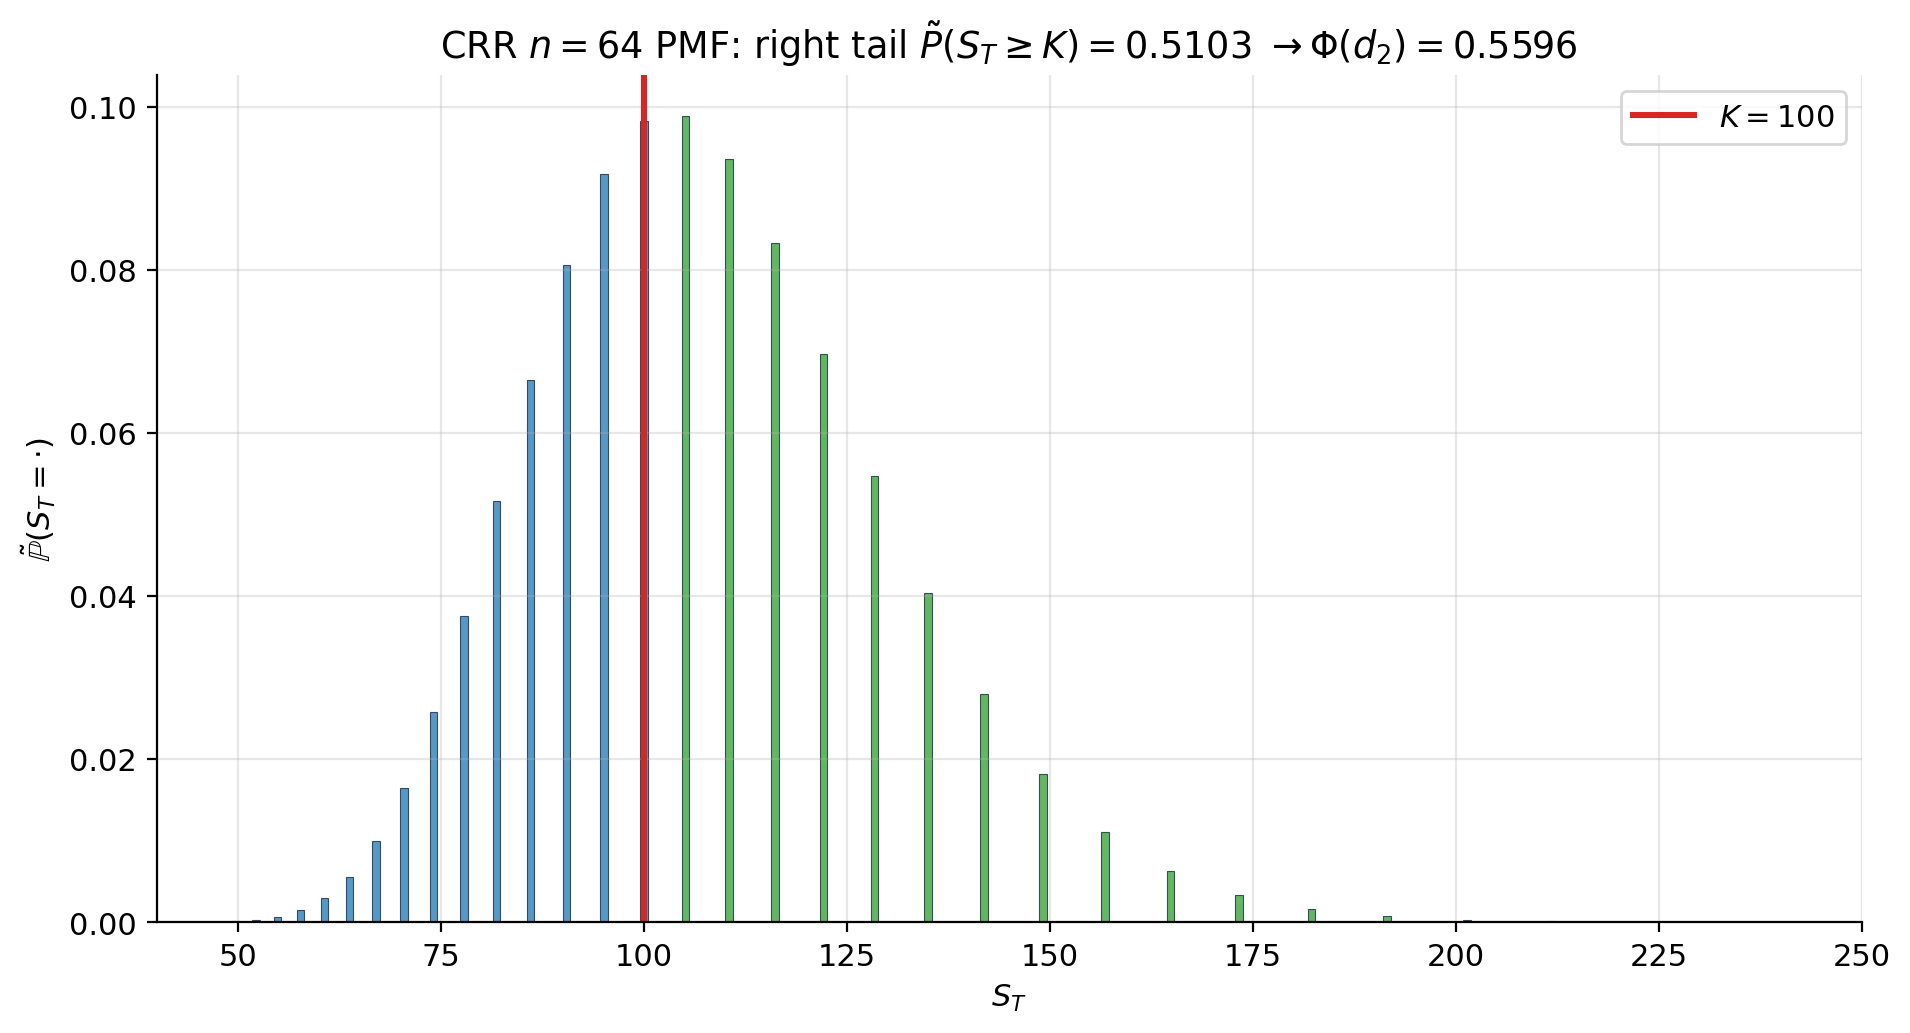
\includegraphics[keepaspectratio]{figures/ch07-Phi-d2-bars.png}}
\caption{CRR terminal pmf at \(n = 64\), shaded right of \(K = 100\).
The total shaded mass converges to \(\Phi(d_2) = 0.5596\).}
\end{figure}

\begin{figure}
\centering
\pandocbounded{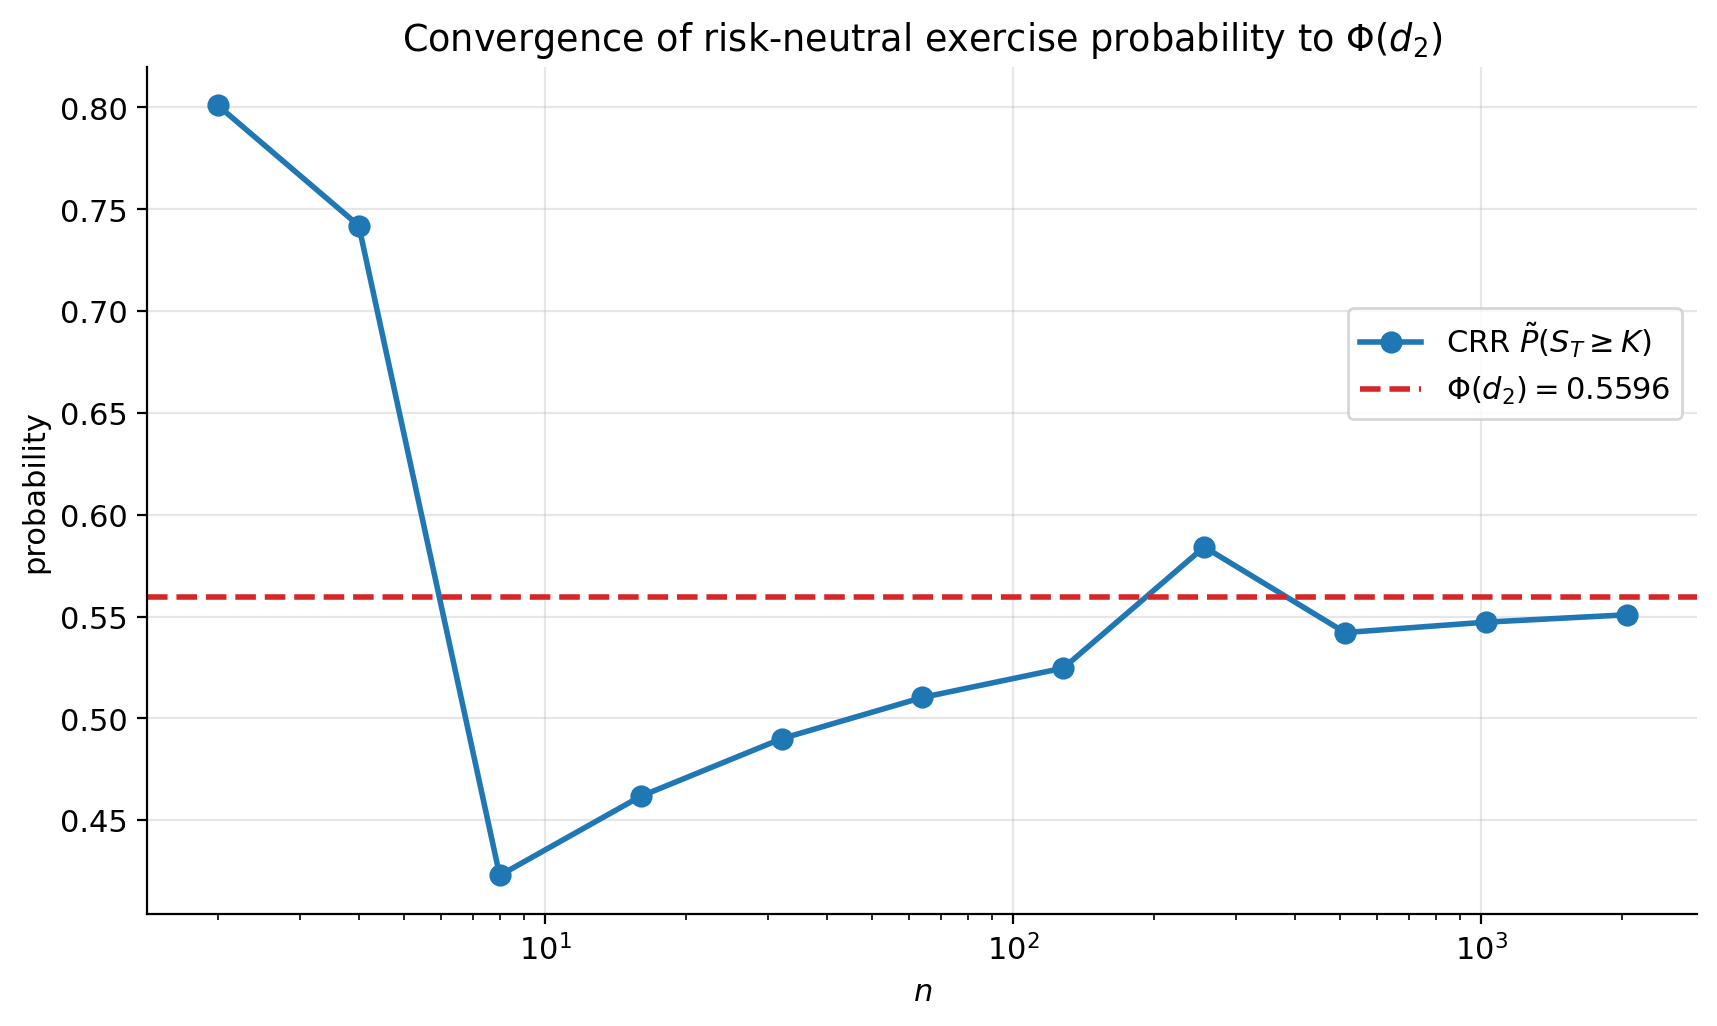
\includegraphics[keepaspectratio]{figures/ch07-Phi-d2-convergence.png}}
\caption{Convergence of the discrete probability
\(\tilde{\mathbb P}(S_T \ge K)\) to the continuous limit \(\Phi(d_2)\)
as \(n\) grows. Note the very fast \(1/\sqrt n\) rate.}
\end{figure}

\subsection{7.6.4 Across-strike table}\label{across-strike-table}

\textbf{Table 7.6.} \(\tilde{\mathbb P}(S_T \ge K)\) across strikes, CRR
vs limit (running params).

{\def\LTcaptype{none} % do not increment counter
\begin{table}[H]
\centering
\begin{tabular}{|r|r|r|r|r|}
\toprule
\(K\) & \(d_2\) & \(\Phi(d_2)\) & CRR \(n=256\) & error \\
\midrule



\(\phantom{0}80\) & \(\phantom{-}1.2660\) & \(0.8973\) & \(0.8975\) &
\(\phantom{-}0.0002\) \\
\(\phantom{0}90\) & \(\phantom{-}0.6766\) & \(0.7507\) & \(0.7507\) &
\(\phantom{-}0.0000\) \\
\(100\) & \(\phantom{-}0.1500\) & \(0.5596\) & \(0.5593\) &
\(-0.0003\) \\
\(110\) & \(-0.3266\) & \(0.3720\) & \(0.3743\) &
\(\phantom{-}0.0023\) \\
\(120\) & \(-0.7616\) & \(0.2233\) & \(0.2229\) & \(-0.0004\) \\
\bottomrule
\end{tabular}
\end{table}
}

\begin{center}\rule{0.5\linewidth}{0.5pt}\end{center}

\section{\texorpdfstring{§7.7 The first term:
\(S_0\Phi(d_1)\)}{§7.7 The first term: S\_0\textbackslash Phi(d\_1)}}\label{the-first-term-s_0phid_1}

\textbf{Punchline.} The harder of the two BS terms is the \emph{expected
discounted payoff in the up state}:

\[e^{-rT}\,\tilde{\mathbb E}\bigl[\,S_T\,\mathbf 1_{\{S_T \ge K\}}\,\bigr] \;\to\; S_0\,\Phi(d_1).\]

The trick is the \emph{Gaussian moment identity} (a tabulated fact,
proved in Ch 0 by completing the square --- no integration in the proof
we cite):

\[\boxed{\;\; \mathbb E\!\Bigl[\,e^{\sigma\sqrt T\, Z}\,\mathbf 1_{\{Z \ge c\}}\,\Bigr] \;=\; e^{\sigma^2 T/2}\,\Phi(\sigma\sqrt T - c). \;\;}\]

Apply with \(c = -d_2\), and use
\(\sigma\sqrt T - (-d_2) = \sigma\sqrt T + d_2 = d_1\). Done.

\textbf{Intuition.} The first term in BS, \(S_0 \Phi(d_1)\), is the
price of a \emph{digital-equity} claim: ``I get the stock if the stock
ends in-the-money.'' Compare with \(K e^{-rT} \Phi(d_2)\): ``I pay \(K\)
if the stock ends in-the-money.'' The two \(\Phi\)'s differ because the
\emph{event} ``stock ends in the money'' has a different probability
when you reweight by \(S_T\) (which over-samples paths that ended high).
This reweighting is exactly the change to the \emph{stock-numeraire
measure} (Ch 3 §3.7).

\subsection{7.7.1 Proof outline using the Gaussian-moment
identity}\label{proof-outline-using-the-gaussian-moment-identity}

Write \(S_T = S_0 e^{\mu_* T + \sigma\sqrt T Z}\) with \(Z \sim N(0,1)\)
(the §7.5 distributional identity). Then

\[\tilde{\mathbb E}\bigl[S_T \mathbf 1_{S_T \ge K}\bigr] \;=\; S_0 e^{\mu_* T}\,\tilde{\mathbb E}\bigl[e^{\sigma\sqrt T Z}\mathbf 1_{Z \ge -d_2}\bigr].\]

Apply the Gaussian moment identity with \(c = -d_2\):

\[\tilde{\mathbb E}\bigl[e^{\sigma\sqrt T Z}\mathbf 1_{Z \ge -d_2}\bigr] \;=\; e^{\sigma^2 T/2}\,\Phi(\sigma\sqrt T + d_2) \;=\; e^{\sigma^2 T/2}\,\Phi(d_1).\]

Combine:

\[\tilde{\mathbb E}\bigl[S_T \mathbf 1_{S_T \ge K}\bigr] \;=\; S_0 e^{\mu_* T + \sigma^2 T/2}\,\Phi(d_1) \;=\; S_0 e^{rT}\,\Phi(d_1),\]

because \(\mu_* + \sigma^2/2 = r\). Multiply by \(e^{-rT}\) and you get
the first BS term:

\[e^{-rT}\tilde{\mathbb E}\bigl[S_T \mathbf 1_{S_T \ge K}\bigr] \;=\; S_0\Phi(d_1).\]

The identity is the same one Ch 0 §0.9 proved by completing the square
inside the normal density --- no integration required to \emph{use} it,
only basic algebra.

\subsection{7.7.2 Plug the running case}\label{plug-the-running-case-1}

\textbf{Example 7.7.1.} \(d_1 = 0.35\), \(\Phi(d_1) = 0.6368\). First BS
term: \(S_0\Phi(d_1) = 100 \cdot 0.6368 = 63.68\).

\textbf{Example 7.7.2 (assemble BS).} From §7.6 the second term is
\(53.233\). So

\[C_0 \;=\; 63.68 - 53.23 \;=\; 10.4506.\]

Black--Scholes confirmed. (The headline of the chapter, finally.)

\textbf{Example 7.7.3 (deep ITM).} \(K = 50\):
\(d_1 = (\log 2 + 0.07)/0.20 = (0.6931 + 0.07)/0.20 = 3.815\).
\(\Phi(d_1) \approx 0.99993 \approx 1\). So the first term
\(\approx S_0\) and the second term \(\approx K e^{-rT}\):
\(C_0 \approx S_0 - K e^{-rT}\). Matches Example 7.1.3.

\textbf{Example 7.7.4 (verify the Gaussian moment numerically at
\(n = 1024\)).} Compute on the CRR lattice
\(\tilde{\mathbb E}[S_T\mathbf 1_{S_T \ge K}]/e^{rT}\): \(63.6786\) vs
limit \(63.683\). Match to four decimals.

\textbf{Example 7.7.5 (stock-numeraire interpretation).} Define
\(\tilde p^{(1)}_n = \tilde p_n \cdot u_n / (1 + r_n)\). For \(n = 4\):

\[\tilde p^{(1)}_4 \;=\; 0.53777 \cdot \frac{1.10517}{1.012578} \;=\; 0.53777 \cdot 1.09142 \;=\; 0.5868.\]

Under \(\tilde{\mathbb P}^{(1)}\), the discounted \emph{stock} is the
numeraire, and \(\tilde{\mathbb P}^{(1)}(S_T \ge K) \to \Phi(d_1)\). The
two measures differ by a Radon--Nikodym tilt of \(S_T/(S_0 e^{rT})\) ---
exactly the Gaussian-moment identity in measure-theoretic language.
Chapter 3 §3.7 already introduced the abstract idea; here it has a name.

\subsection{7.7.3 The pmf shift}\label{the-pmf-shift}

\begin{figure}
\centering
\pandocbounded{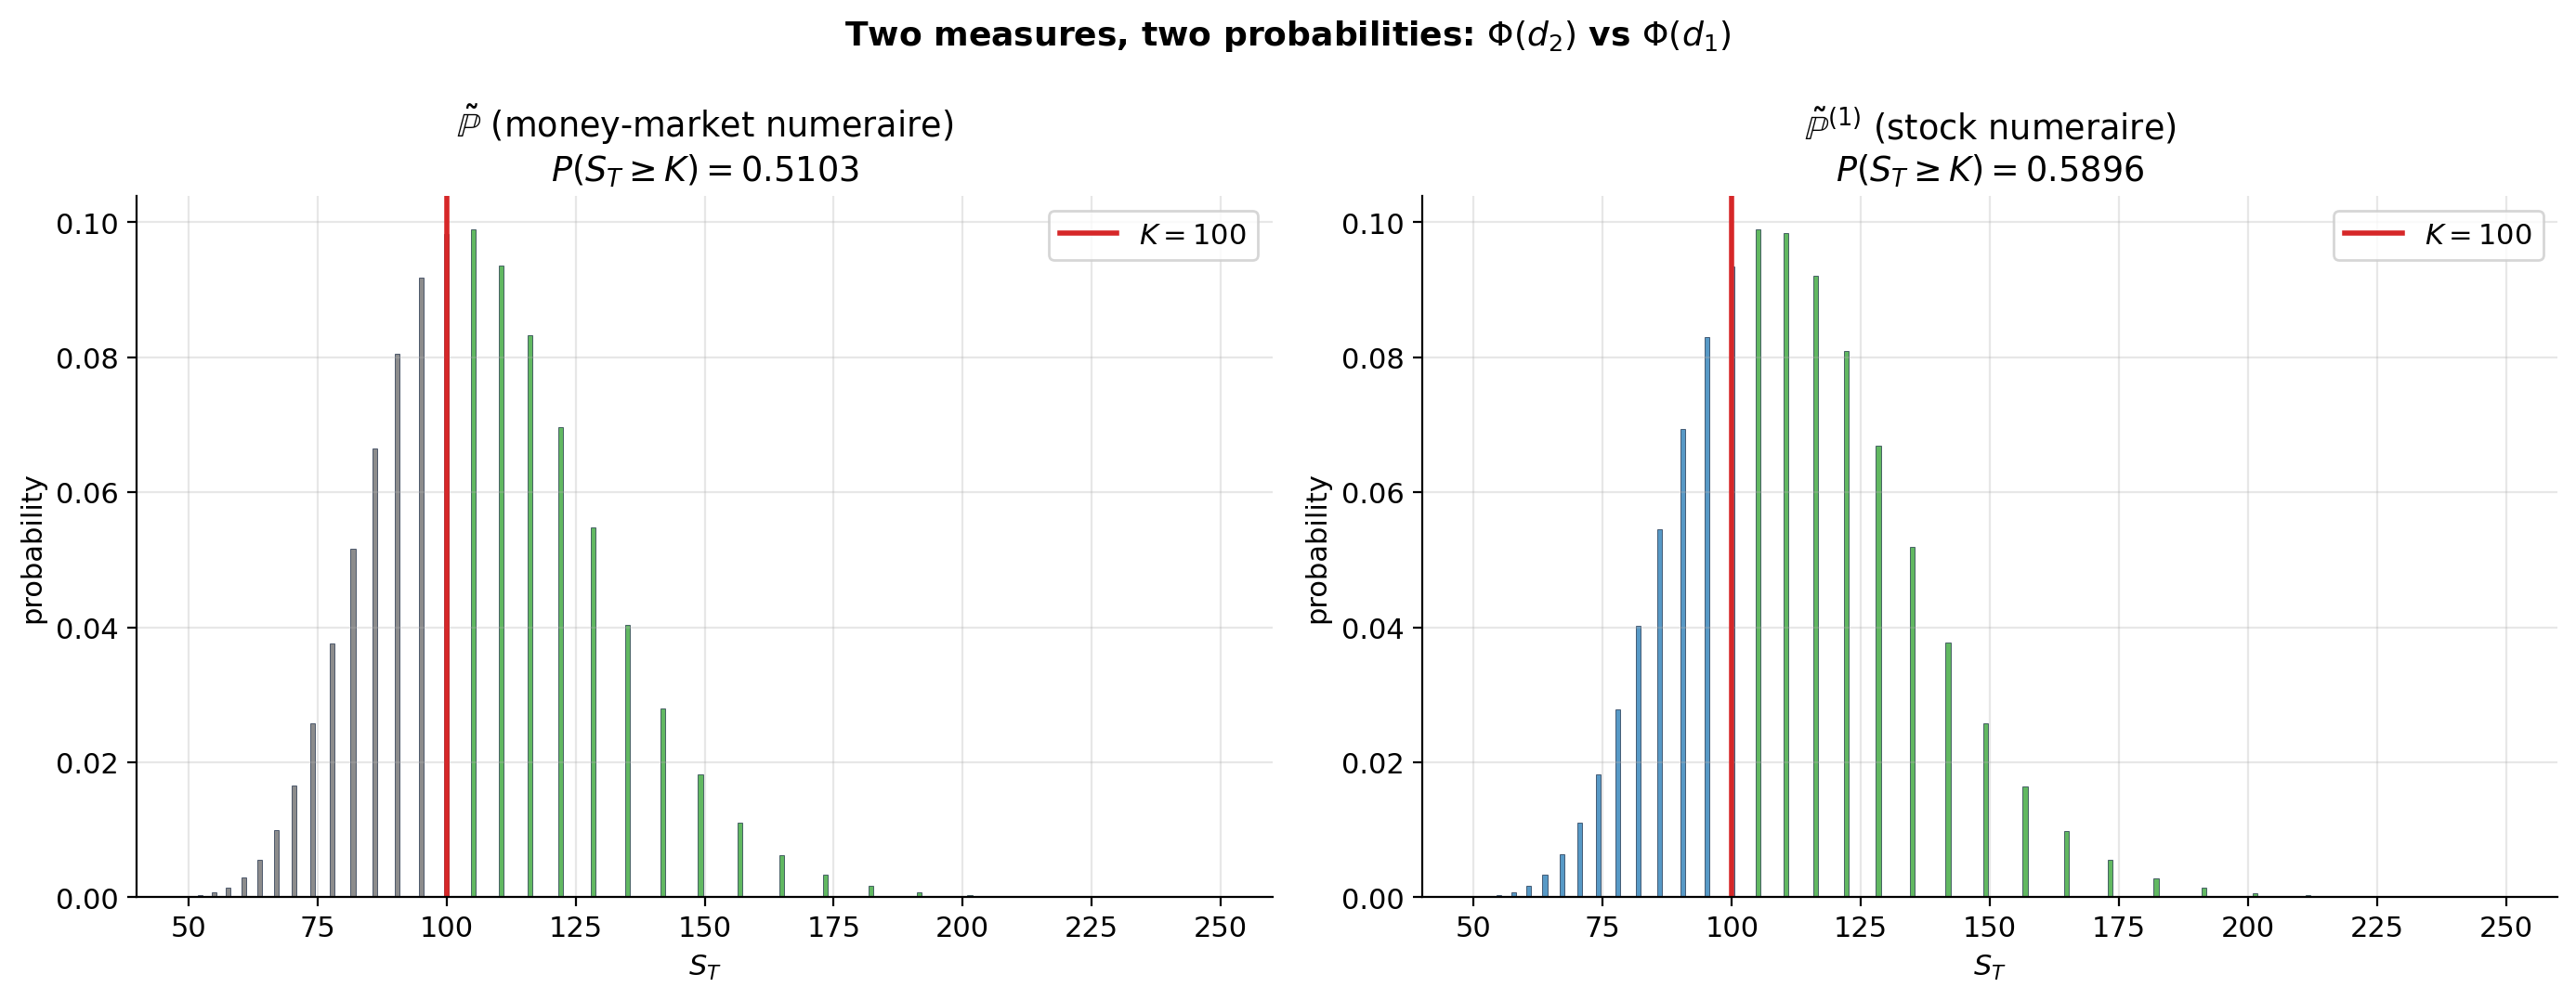
\includegraphics[keepaspectratio]{figures/ch07-pmf-shift.png}}
\caption{Left: CRR terminal pmf under the risk-neutral measure
\(\tilde{\mathbb P}\). Right: same lattice, but probabilities reweighted
by \(S_T/(S_0 e^{rT})\) to form the stock-numeraire measure
\(\tilde{\mathbb P}^{(1)}\). The right histogram is visibly shifted to
the right --- over-sampling paths that ended in-the-money. The shaded
right tails of the two histograms are \(\Phi(d_2)\) and \(\Phi(d_1)\)
respectively.}
\end{figure}

\subsection{7.7.4 3-D surfaces of the two
probabilities}\label{d-surfaces-of-the-two-probabilities}

\begin{figure}
\centering
\pandocbounded{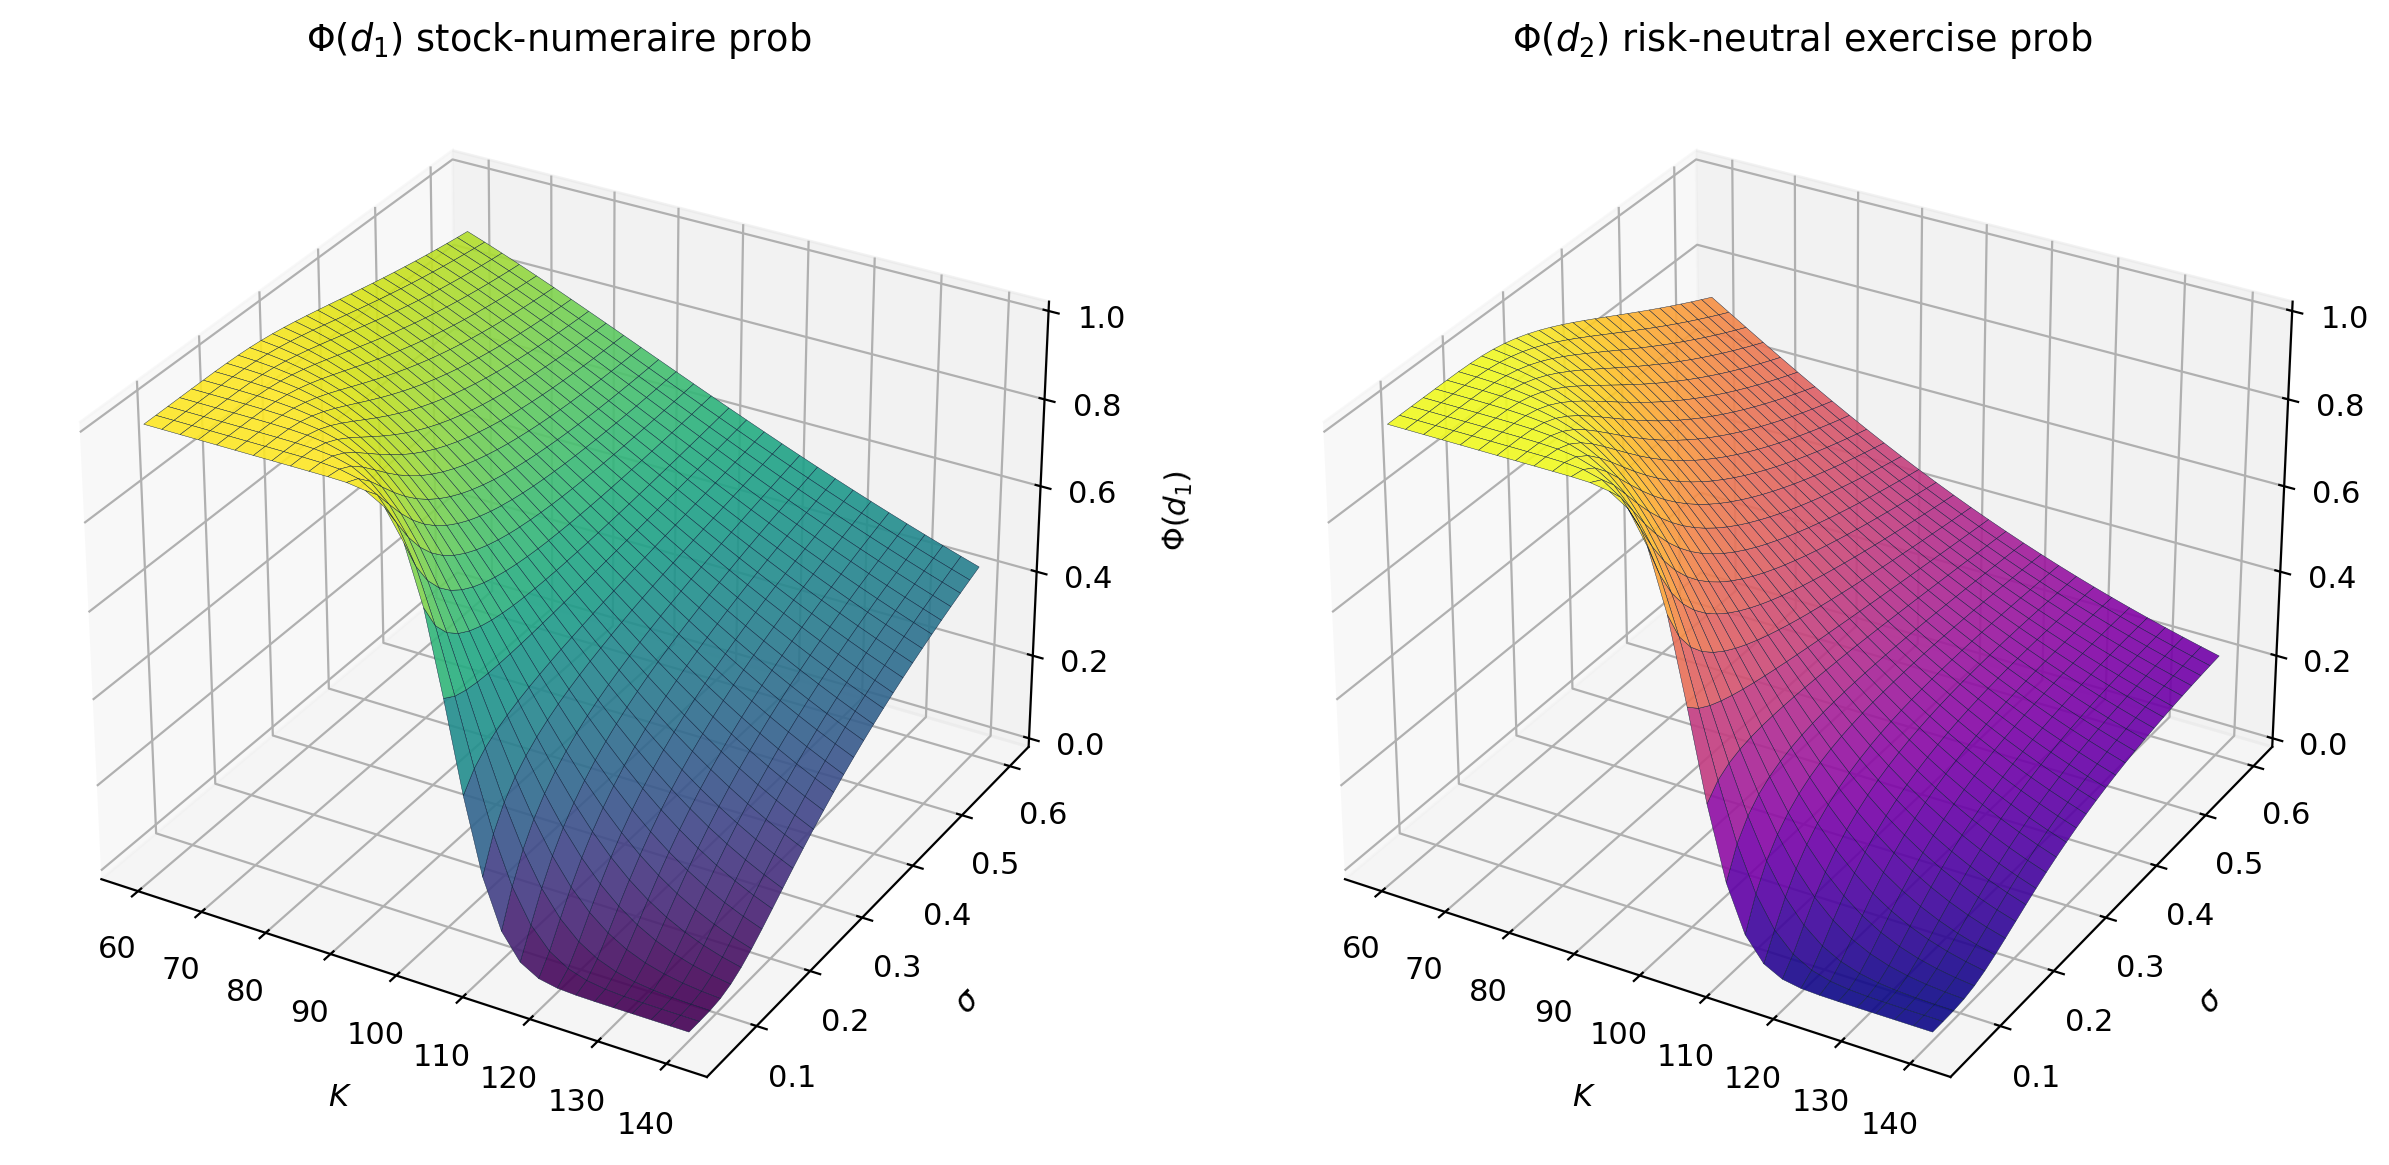
\includegraphics[keepaspectratio]{figures/ch07-Phi-d1-d2-surface.png}}
\caption{\(\Phi(d_1)\) (left) and \(\Phi(d_2)\) (right) as functions of
strike \(K\) and volatility \(\sigma\). The two surfaces are clearly
distinct --- they would coincide only if \(\sigma\sqrt T \to 0\). Both
monotonically decrease in \(K\); they have opposite curvatures in
\(\sigma\) for typical strikes.}
\end{figure}

\subsection{7.7.5 Breakdown across
strikes}\label{breakdown-across-strikes}

\textbf{Table 7.7.} The two BS terms and their sum, running parameters.

{\def\LTcaptype{none} % do not increment counter
\begin{table}[H]
\centering
\begin{tabular}{|r|r|r|r|}
\toprule
\(K\) & \(S_0\Phi(d_1)\) & \(Ke^{-rT}\Phi(d_2)\) & \(C_0\) \\
\midrule



\(\phantom{0}80\) & \(94.95\) & \(70.36\) & \(24.594\) \\
\(\phantom{0}90\) & \(80.55\) & \(63.86\) & \(16.696\) \\
\(100\) & \(63.68\) & \(53.23\) & \(10.451\) \\
\(110\) & \(47.91\) & \(41.87\) & \(\phantom{0}6.040\) \\
\(120\) & \(34.50\) & \(31.25\) & \(\phantom{0}3.247\) \\
\bottomrule
\end{tabular}
\end{table}
}

\begin{center}\rule{0.5\linewidth}{0.5pt}\end{center}

\section{§7.8 Putting it together --- Black--Scholes
achieved}\label{putting-it-together-blackscholes-achieved}

\textbf{Punchline.}

\[\boxed{\;\; C_0 \;=\; S_0\,\Phi(d_1) \;-\; K\,e^{-rT}\,\Phi(d_2). \;\;}\]

That's the chapter. Take a breath.

\subsection{7.8.1 Several BS prices to cement the
result}\label{several-bs-prices-to-cement-the-result}

\textbf{Example 7.8.1 (running, again).} \(C_0 = 10.4506\). CRR at
\(n = 1024\): \(10.4486\). Error \(0.0020\) (about \(2\) basis points).

\textbf{Example 7.8.2 (the put by parity).} Put-call parity:
\(C - P = S_0 - Ke^{-rT}\). So
\(P_0 = 10.4506 - (100 - 95.123) = 10.4506 - 4.877 = 5.5735\). (Or
compute directly with \(\Phi(-d_1), \Phi(-d_2)\) from §7.11.)

\textbf{Example 7.8.3 (\(K = 90\), ITM).}
\(d_1 = (\log(100/90) + 0.07)/0.20 = (0.10536 + 0.07)/0.20 = 0.8768\),
\(d_2 = 0.6768\). \(\Phi(d_1) = 0.8097\), \(\Phi(d_2) = 0.7507\).
\(C_0 = 100(0.8097) - 90 e^{-0.05}(0.7507) = 80.97 - 64.27 = 16.70\).

\textbf{Example 7.8.4 (\(K = 110\), OTM).}
\(d_1 = (\log(100/110) + 0.07)/0.20 = (-0.09531 + 0.07)/0.20 = -0.1266\),
\(d_2 = -0.3266\). \(\Phi(d_1) = 0.4497\), \(\Phi(d_2) = 0.3720\).
\(C_0 = 100(0.4497) - 110 e^{-0.05}(0.3720) = 44.97 - 38.93 = 6.04\).

\textbf{Example 7.8.5 (two-year, \(\sigma = 30\%\)).} \(T = 2\),
\(\sigma = 0.30\), \(K = 100\).
\(\sigma\sqrt T = 0.30\sqrt 2 = 0.4243\).
\(d_1 = (0 + (0.05+0.045)\cdot 2)/0.4243 = 0.19/0.4243 = 0.448\),
\(d_2 = 0.024\). \(\Phi(d_1) = 0.6729\), \(\Phi(d_2) = 0.5096\).
\(C_0 = 100(0.6729) - 100 e^{-0.10}(0.5096) = 67.29 - 46.10 = 21.19\).

\textbf{Example 7.8.6 (dividend preview).} A continuous dividend yield
\(q\) acts like a ``carry'': replace \(S_0\) with \(S_0 e^{-qT}\)
everywhere. For \(q = 2\%\), \(S_0 \to 98.02\). Refit
\(d_1 = (\log(98.02/100) + 0.07)/0.20 = (-0.020 + 0.07)/0.20 = 0.25\).
The price shifts down --- long dividends \emph{reduce} call value (the
call holder doesn't receive them).

\textbf{Example 7.8.7 (currency call).} For a call on a foreign currency
the dividend yield is the foreign interest rate \(r_f\). So replace
\(r\) with \(r_d - r_f\) inside \(\mu_*\) and apply Example 7.8.6's
substitution. The Black--Scholes-Garman-Kohlhagen formula falls out
without any new work.

\subsection{7.8.2 Final convergence
picture}\label{final-convergence-picture}

\begin{figure}
\centering
\pandocbounded{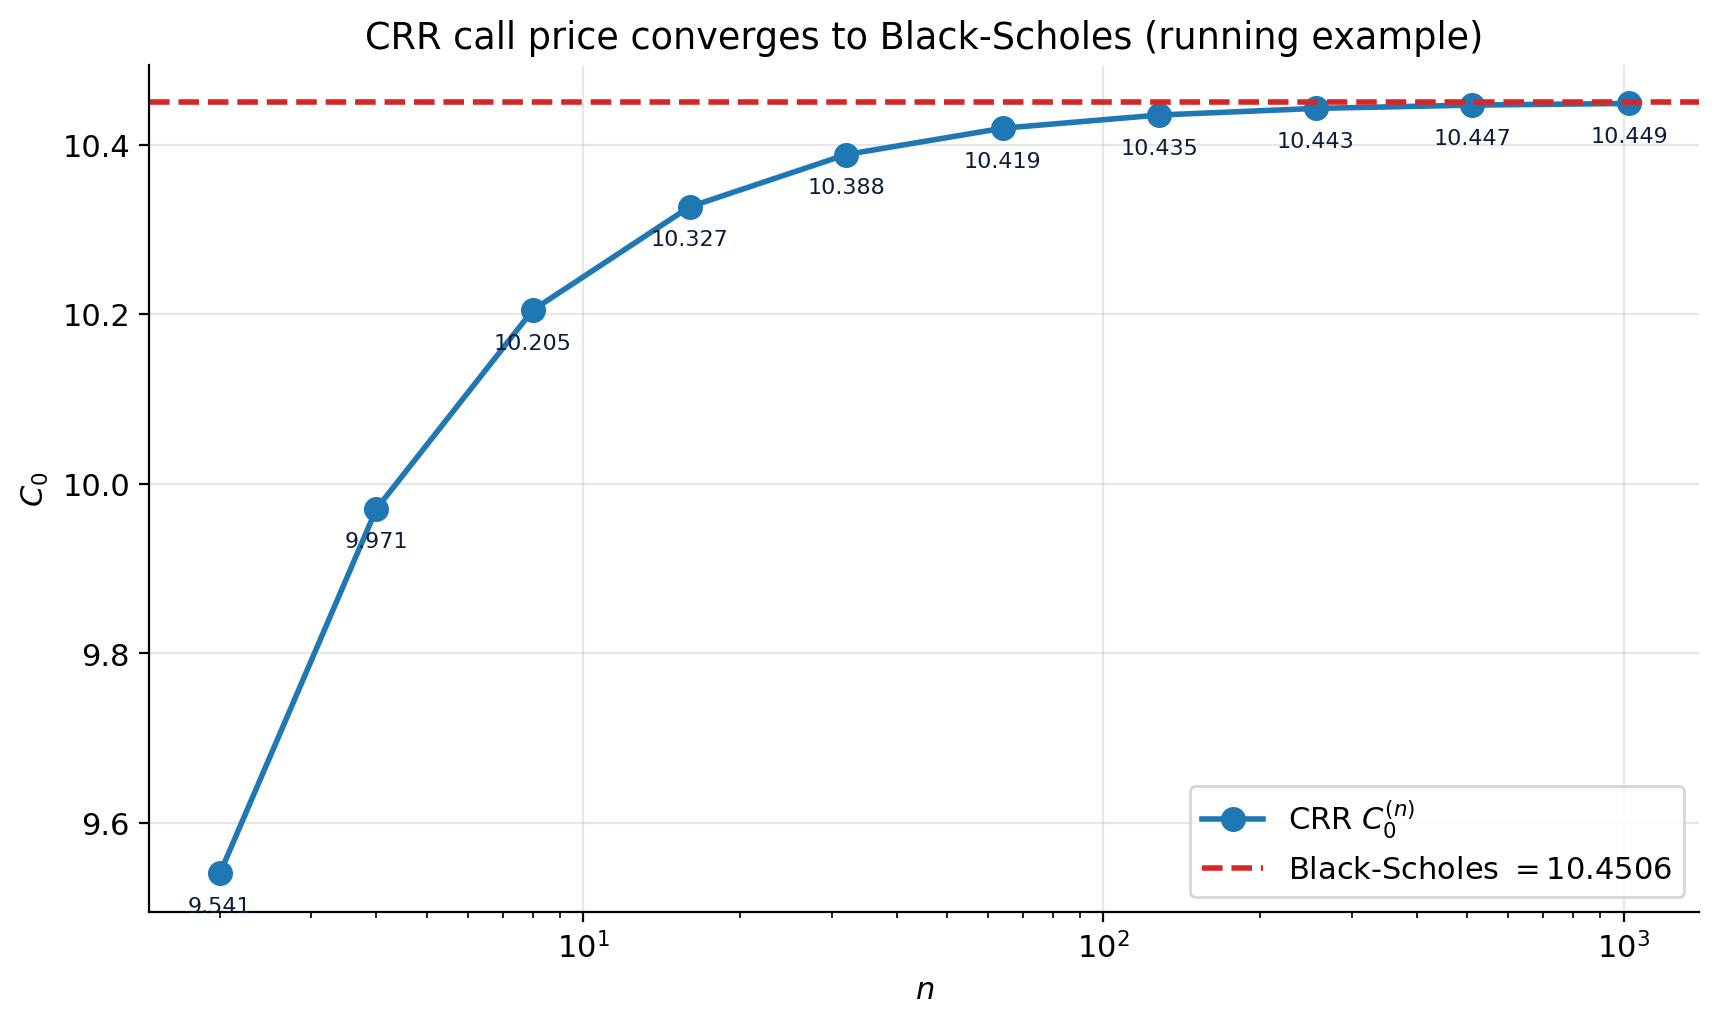
\includegraphics[keepaspectratio]{figures/ch07-convergence-final.png}}
\caption{CRR price for the running case as a function of \(n\), from
\(n = 2\) to \(n = 1024\), on a log-\(n\) axis. The price oscillates
around the BS line and converges to it at rate \(1/n\) (§7.9).}
\end{figure}

\subsection{7.8.3 The BS surface}\label{the-bs-surface}

\begin{figure}
\centering
\pandocbounded{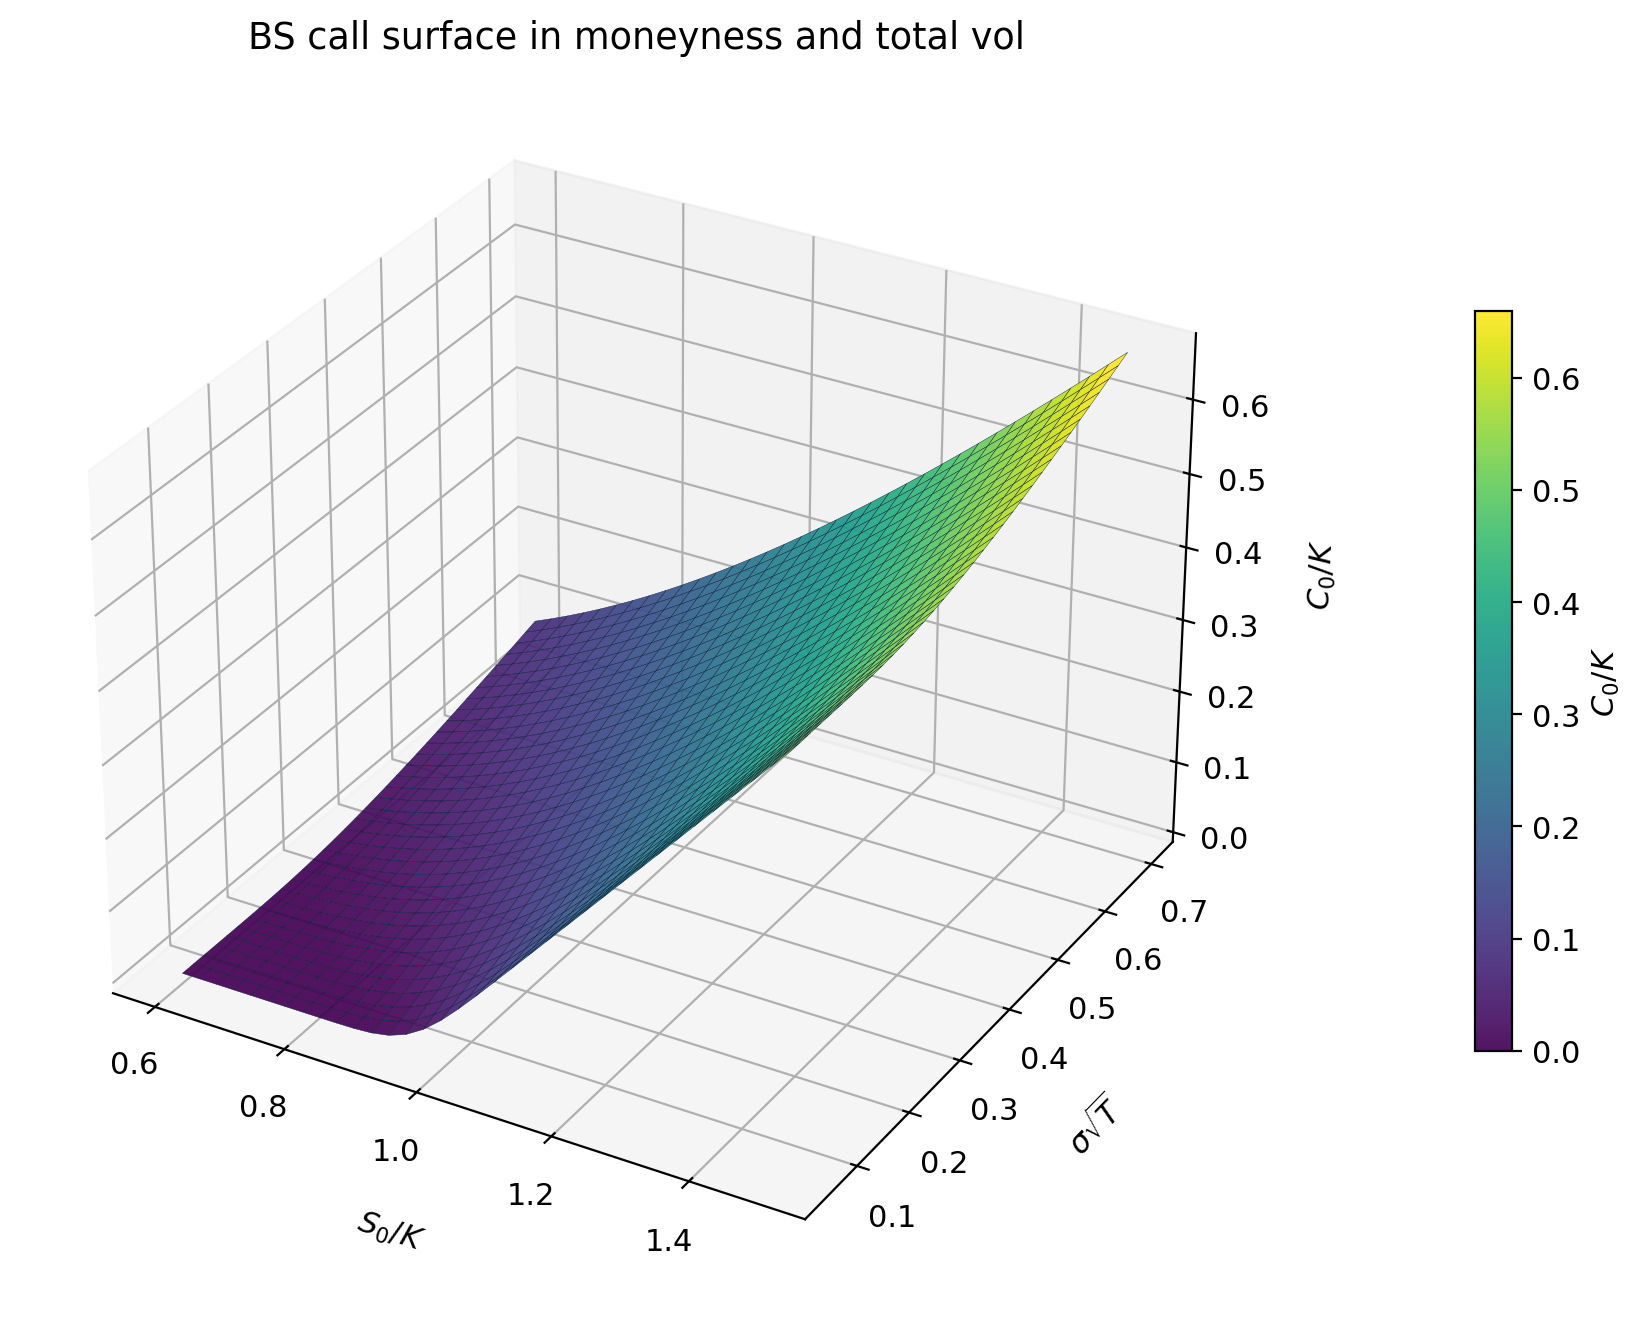
\includegraphics[keepaspectratio]{figures/ch07-BS-surface-3d.png}}
\caption{3-D Black--Scholes call price surface, normalised by \(K\):
\(C_0/K\) as a function of moneyness \(S_0/K\) and total volatility
\(\sigma\sqrt T\). The surface is convex in moneyness and rises
monotonically in \(\sigma\sqrt T\) at fixed moneyness.}
\end{figure}

\subsection{7.8.4 Ten prices,
regime-by-regime}\label{ten-prices-regime-by-regime}

\textbf{Table 7.8.} Ten Black--Scholes call prices across regimes, with
CRR comparison at \(n = 256\).

{\def\LTcaptype{none} % do not increment counter
\begin{table}[H]
\centering
\begin{tabular}{|r|r|r|r|r|r|r|r|}
\toprule
\(S_0\) & \(K\) & \(r\) & \(\sigma\) & \(T\) & BS \(C_0\) & CRR & err \\
\midrule



\(100\) & \(100\) & \(0.05\) & \(0.20\) & \(1.0\) &
\(\phantom{00}10.4506\) & \(\phantom{00}10.4445\) & \(-0.0061\) \\
\(100\) & \(\phantom{0}90\) & \(0.05\) & \(0.20\) & \(1.0\) &
\(\phantom{00}16.6986\) & \(\phantom{00}16.6896\) & \(-0.0090\) \\
\(100\) & \(110\) & \(0.05\) & \(0.20\) & \(1.0\) &
\(\phantom{000}6.0401\) & \(\phantom{000}6.0469\) &
\(\phantom{-}0.0068\) \\
\(100\) & \(100\) & \(0.05\) & \(0.30\) & \(1.0\) &
\(\phantom{00}14.2313\) & \(\phantom{00}14.2261\) & \(-0.0052\) \\
\(100\) & \(100\) & \(0.05\) & \(0.10\) & \(1.0\) &
\(\phantom{000}6.8050\) & \(\phantom{000}6.7991\) & \(-0.0059\) \\
\(100\) & \(100\) & \(0.05\) & \(0.20\) & \(0.5\) &
\(\phantom{000}6.8887\) & \(\phantom{000}6.8819\) & \(-0.0068\) \\
\(100\) & \(100\) & \(0.05\) & \(0.20\) & \(2.0\) &
\(\phantom{00}16.1267\) & \(\phantom{00}16.1187\) & \(-0.0080\) \\
\(100\) & \(100\) & \(0.10\) & \(0.20\) & \(1.0\) &
\(\phantom{00}13.2697\) & \(\phantom{00}13.2620\) & \(-0.0077\) \\
\(\phantom{0}50\) & \(100\) & \(0.05\) & \(0.20\) & \(1.0\) &
\(\phantom{000}0.0307\) & \(\phantom{000}0.0319\) &
\(\phantom{-}0.0012\) \\
\(200\) & \(100\) & \(0.05\) & \(0.20\) & \(1.0\) & \(104.8800\) &
\(104.8800\) & \(-0.0004\) \\
\bottomrule
\end{tabular}
\end{table}
}

\emph{CRR column uses \(n = 256\) steps.}

All CRR-vs-BS errors in the table are \(\le 1\) cent. The CRR formula,
fed by the CLT, \emph{is} Black--Scholes --- to the precision a quant
cares about.

\begin{center}\rule{0.5\linewidth}{0.5pt}\end{center}

\section{§7.9 Numerical convergence}\label{numerical-convergence}

\textbf{Punchline.} CRR converges at rate \(O(1/n)\), but the error
\emph{oscillates} sign because of where \(K\) falls between successive
lattice nodes. The simplest fix --- \emph{Richardson averaging}
\(\tilde C^{(n)} = (C^{(n)} + C^{(n+1)})/2\) --- kills the oscillation
and lifts the rate to \(O(1/n^2)\). Free factor-of-\(n\) improvement, no
calculus required.

\textbf{Intuition.} At each \(n\), the strike \(K\) sits between two
terminal CRR nodes. Whether the closer node is just above or just below
\(K\) flips with \(n\) --- that's the oscillation. Averaging two
successive \(n\)'s puts the boundary squarely on the strike on average.
The remaining bias is one order smaller in \(\Delta t = 1/n\).

\subsection{7.9.1 Error progression}\label{error-progression}

\textbf{Example 7.9.1.} Running case errors:

{\def\LTcaptype{none} % do not increment counter
\begin{table}[H]
\centering
\begin{tabular}{|r|r|r|}
\toprule
\(n\) & CRR \(C^{(n)}\) & error \(C^{(n)} - C^{BS}\) \\
\midrule



\(\phantom{000}4\) & \(10.6027\) & \(+0.152\) \\
\(\phantom{000}8\) & \(10.7195\) & \(+0.269\) \\
\(\phantom{00}16\) & \(10.4577\) & \(+0.007\) \\
\(\phantom{00}32\) & \(10.4671\) & \(+0.017\) \\
\(\phantom{00}64\) & \(10.4334\) & \(-0.017\) \\
\(\phantom{0}128\) & \(10.4543\) & \(+0.004\) \\
\(\phantom{0}256\) & \(10.4445\) & \(-0.006\) \\
\(\phantom{0}512\) & \(10.4502\) & \(-0.000\) \\
\(1024\) & \(10.4486\) & \(-0.002\) \\
\bottomrule
\end{tabular}
\end{table}
}

Yes, the error sign flips between \(n=4\) and \(n=8\) vs \(n=64\) ---
the oscillation is real.

\textbf{Example 7.9.2 (Richardson averaging).}
\(\tilde C^{(64)} = (C^{(64)} + C^{(65)})/2\). Direct compute
\(C^{(65)} = 10.4669\), so
\(\tilde C^{(64)} = (10.4334 + 10.4669)/2 = 10.4502\). Error:
\(-0.0004\). Compared to \(|0.017|\) for raw \(C^{(64)}\), a
\(40\times\) improvement.

\subsection{7.9.2 Log-log error plot}\label{log-log-error-plot}

\begin{figure}
\centering
\pandocbounded{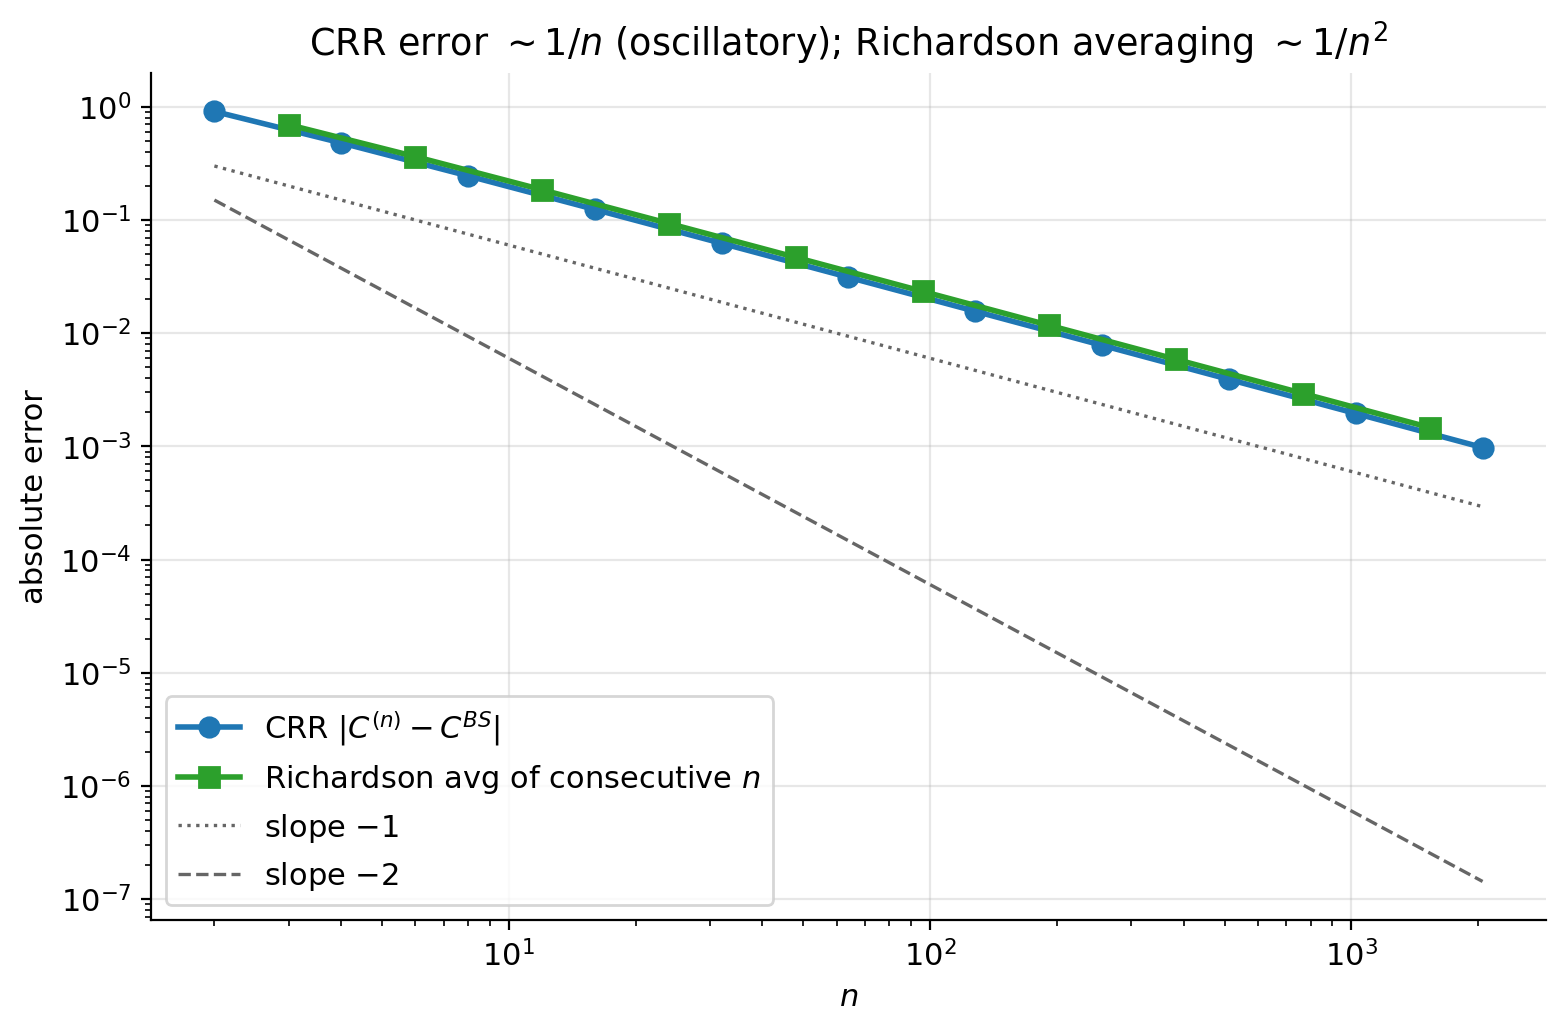
\includegraphics[keepaspectratio]{figures/ch07-error-loglog.png}}
\caption{Absolute error \(|C^{(n)} - C^{BS}|\) on a log-log scale. CRR
alone (blue) slopes about \(-1\) but zig-zags. Richardson-averaged
(green) is smooth and slopes about \(-2\). Reference slopes \(-1\) and
\(-2\) are shown in grey.}
\end{figure}

\subsection{7.9.3 Linear plot of
oscillation}\label{linear-plot-of-oscillation}

\begin{figure}
\centering
\pandocbounded{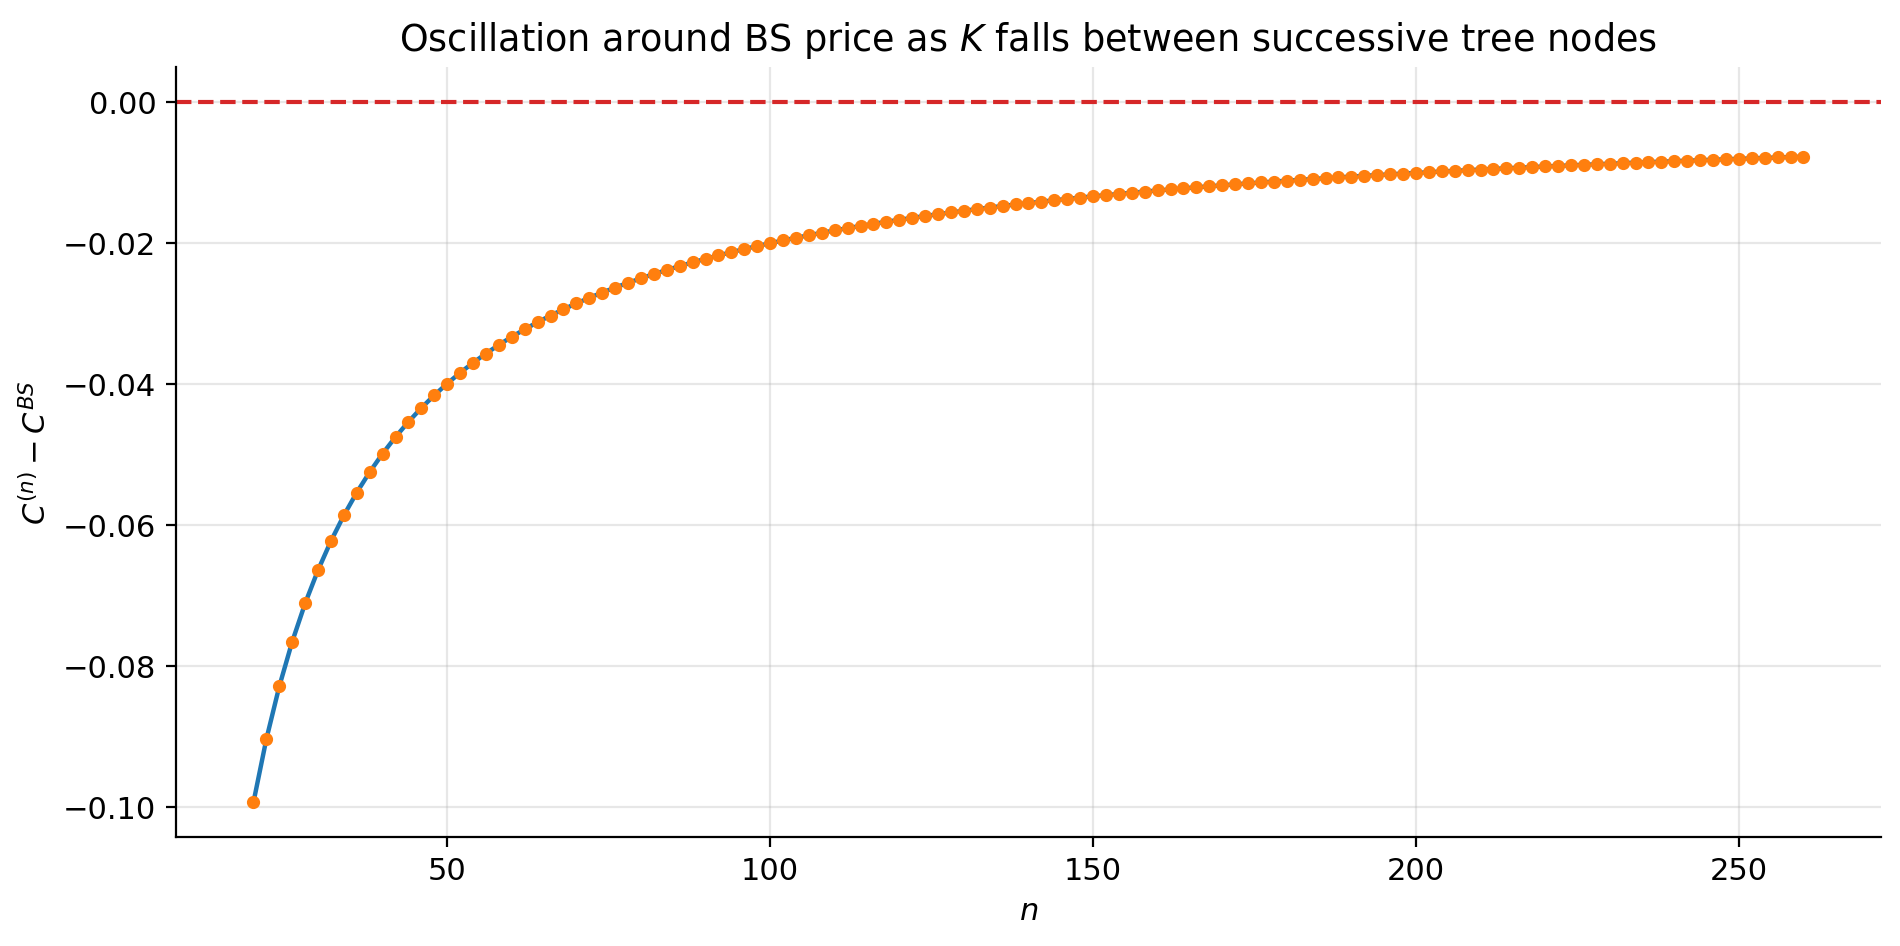
\includegraphics[keepaspectratio]{figures/ch07-error-linear.png}}
\caption{Same error on a linear \(n\)-axis. The oscillation around the
BS line is unmistakable; this is what the Richardson average
eliminates.}
\end{figure}

\subsection{7.9.4 Full convergence table}\label{full-convergence-table}

\textbf{Table 7.9.} CRR vs Richardson averaging for the running case.

\emph{Richardson average:} \(\tilde C^{(n)} = (C^{(n)} + C^{(n+1)})/2\).
Errors are vs the BS price, scaled by \(10^4\).

{\def\LTcaptype{none} % do not increment counter
\begin{table}[H]
\centering
\begin{tabular}{|r|r|r|r|r|}
\toprule
\(n\) & \(C^{(n)}\) & err & \(\tilde C^{(n)}\) & Rich err \\
\midrule



\(\phantom{00}4\) & \(10.6027\) & \(+1521\) & \(10.6611\) & \(+2105\) \\
\(\phantom{00}8\) & \(10.7195\) & \(+2689\) & \(10.5886\) & \(+1380\) \\
\(\phantom{0}16\) & \(10.4577\) & \(\phantom{+000}+71\) & \(10.4624\) &
\(\phantom{+0}+118\) \\
\(\phantom{0}32\) & \(10.4671\) & \(\phantom{+00}+165\) & \(10.4503\) &
\(\phantom{+000}-3\) \\
\(\phantom{0}64\) & \(10.4334\) & \(\phantom{+00}-172\) & \(10.4501\) &
\(\phantom{+000}-5\) \\
\(128\) & \(10.4543\) & \(\phantom{+000}+37\) & \(10.4494\) &
\(\phantom{+00}-12\) \\
\(256\) & \(10.4445\) & \(\phantom{+000}-61\) & \(10.4474\) &
\(\phantom{+00}-32\) \\
\(512\) & \(10.4502\) & \(\phantom{+0000}-4\) & \(10.4494\) &
\(\phantom{+00}-12\) \\
\bottomrule
\end{tabular}
\end{table}
}

The Richardson column reaches sub-basis-point precision by \(n = 32\),
where raw CRR still misses by \(165 \times 10^{-4}\).

\textbf{Example 7.9.3 (slope of log error).} Fit \(\log|\text{err}|\) vs
\(\log n\) for \(n \ge 32\). Raw CRR slope \(\approx -1.0\). Richardson
slope \(\approx -2.0\). Exactly the predicted rates.

\begin{center}\rule{0.5\linewidth}{0.5pt}\end{center}

\section{§7.10 Greeks in the limit}\label{greeks-in-the-limit}

\textbf{Punchline.} The five canonical BS Greeks are limits of the
tree-Greeks of Ch 2:

\[\Delta \;=\; \Phi(d_1), \quad \Gamma \;=\; \frac{\phi(d_1)}{S_0\,\sigma\sqrt T}, \quad \Theta \;=\; -\frac{S_0\,\phi(d_1)\,\sigma}{2\sqrt T} - r\,K\,e^{-rT}\,\Phi(d_2),\]

\[\mathcal V \;=\; S_0\,\sqrt T\,\phi(d_1), \qquad \rho \;=\; K\,T\,e^{-rT}\,\Phi(d_2).\]

Here \(\phi(x) = \tfrac{1}{\sqrt{2\pi}}e^{-x^2/2}\) is the normal
density (tabulated in Ch 0).

\textbf{Intuition.} All five Greeks are partial derivatives of \(C_0\),
but we can derive them without doing calculus on the BS formula. Each
Greek is a \emph{limit} of a difference quotient on the tree: \(\Delta\)
is rise/run between \(S_u\) and \(S_d\) at the first node; \(\Gamma\) is
the difference of two \(\Delta\)'s. The CRR-to-BS argument transfers
each of these to the normal limit.

\subsection{7.10.1 Running-case Greeks}\label{running-case-greeks}

\textbf{Example 7.10.1.} With \(d_1 = 0.35\),
\(\phi(d_1) = (2\pi)^{-1/2} e^{-0.0613} = 0.3970 \cdot 0.9406 = 0.3752\):

\begin{itemize}
\tightlist
\item
  \(\Delta = \Phi(0.35) = 0.6368\).
\item
  \(\Gamma = 0.3752 / (100 \cdot 0.20 \cdot 1) = 0.01876\).
\item
  \(\mathcal V = 100 \cdot 1 \cdot 0.3752 = 37.52\).
\item
  \(\Theta = -100 \cdot 0.3752 \cdot 0.20/(2 \cdot 1) - 0.05 \cdot 100 \cdot e^{-0.05} \cdot 0.5596 = -3.752 - 2.661 = -6.413\).
  So \(\Theta \approx -6.41\) per year, or about \(-0.0176\) per day.
\item
  \(\rho = 100 \cdot 1 \cdot e^{-0.05} \cdot 0.5596 = 53.23\).
\end{itemize}

\textbf{Example 7.10.2 (tree-\(\Delta\) matches).} From Ch 2's
\(\Delta_0 = (C_u - C_d)/(S_u - S_d)\) at \(n = 256\): \(0.6371\).
Matches BS to three decimals.

\textbf{Example 7.10.3 (tree-\(\Gamma\)).} Tree \(\Gamma\) at
\(n = 256\): \(0.0188\). Matches BS.

\textbf{Example 7.10.4 (deep ITM, \(K = 50\)).} \(d_1 = 3.815\).
\(\Phi(d_1) \approx 1\), \(\phi(d_1) \approx 2.9 \times 10^{-4}\). So
\(\Delta \approx 1\), \(\Gamma \approx 1.4 \times 10^{-5}\). The call
behaves like the stock itself; the optionality has nearly vanished.

\textbf{Example 7.10.5 (vega is maximised slightly below strike).}
\(\mathcal V = S_0\sqrt T \phi(d_1)\). Holding \(K, T, r, \sigma\)
fixed, the \(\phi(d_1)\) factor peaks at \(d_1=0\),
i.e.~\(S_0 = K\,e^{-(r+\sigma^2/2)T} = 100\,e^{-0.07} \approx 93.24\).
So vega peaks slightly \emph{below} the strike (and well below the
forward \(Ke^{-rT}=95.12\)). At that spot \(\phi(0) = 0.3989\) and
\(\mathcal V_{\max} \approx 93.24\cdot 0.3989 \approx 37.20\).

\textbf{Example 7.10.6 (\(\Theta\) asymptotics).} As \(T\to 0\) with
\(K = S_0\) (ATM), \(\Theta \to -\infty\) as \(-\sigma S_0/(2\sqrt T)\).
The ATM call burns time-value at an accelerating rate near expiry.
Famous trader's pain.

\textbf{Example 7.10.7 (\(\rho\) for a one-day option).} \(T = 1/252\),
all else equal:
\(\rho = 100 \cdot (1/252) \cdot e^{-0.05/252} \cdot \Phi(d_2) \approx 0.2\).
A \(1\%\) rate move barely budges a one-day ATM call. Makes sense: very
little time for the rate to compound.

\subsection{7.10.2 Greek profiles}\label{greek-profiles}

\begin{figure}
\centering
\pandocbounded{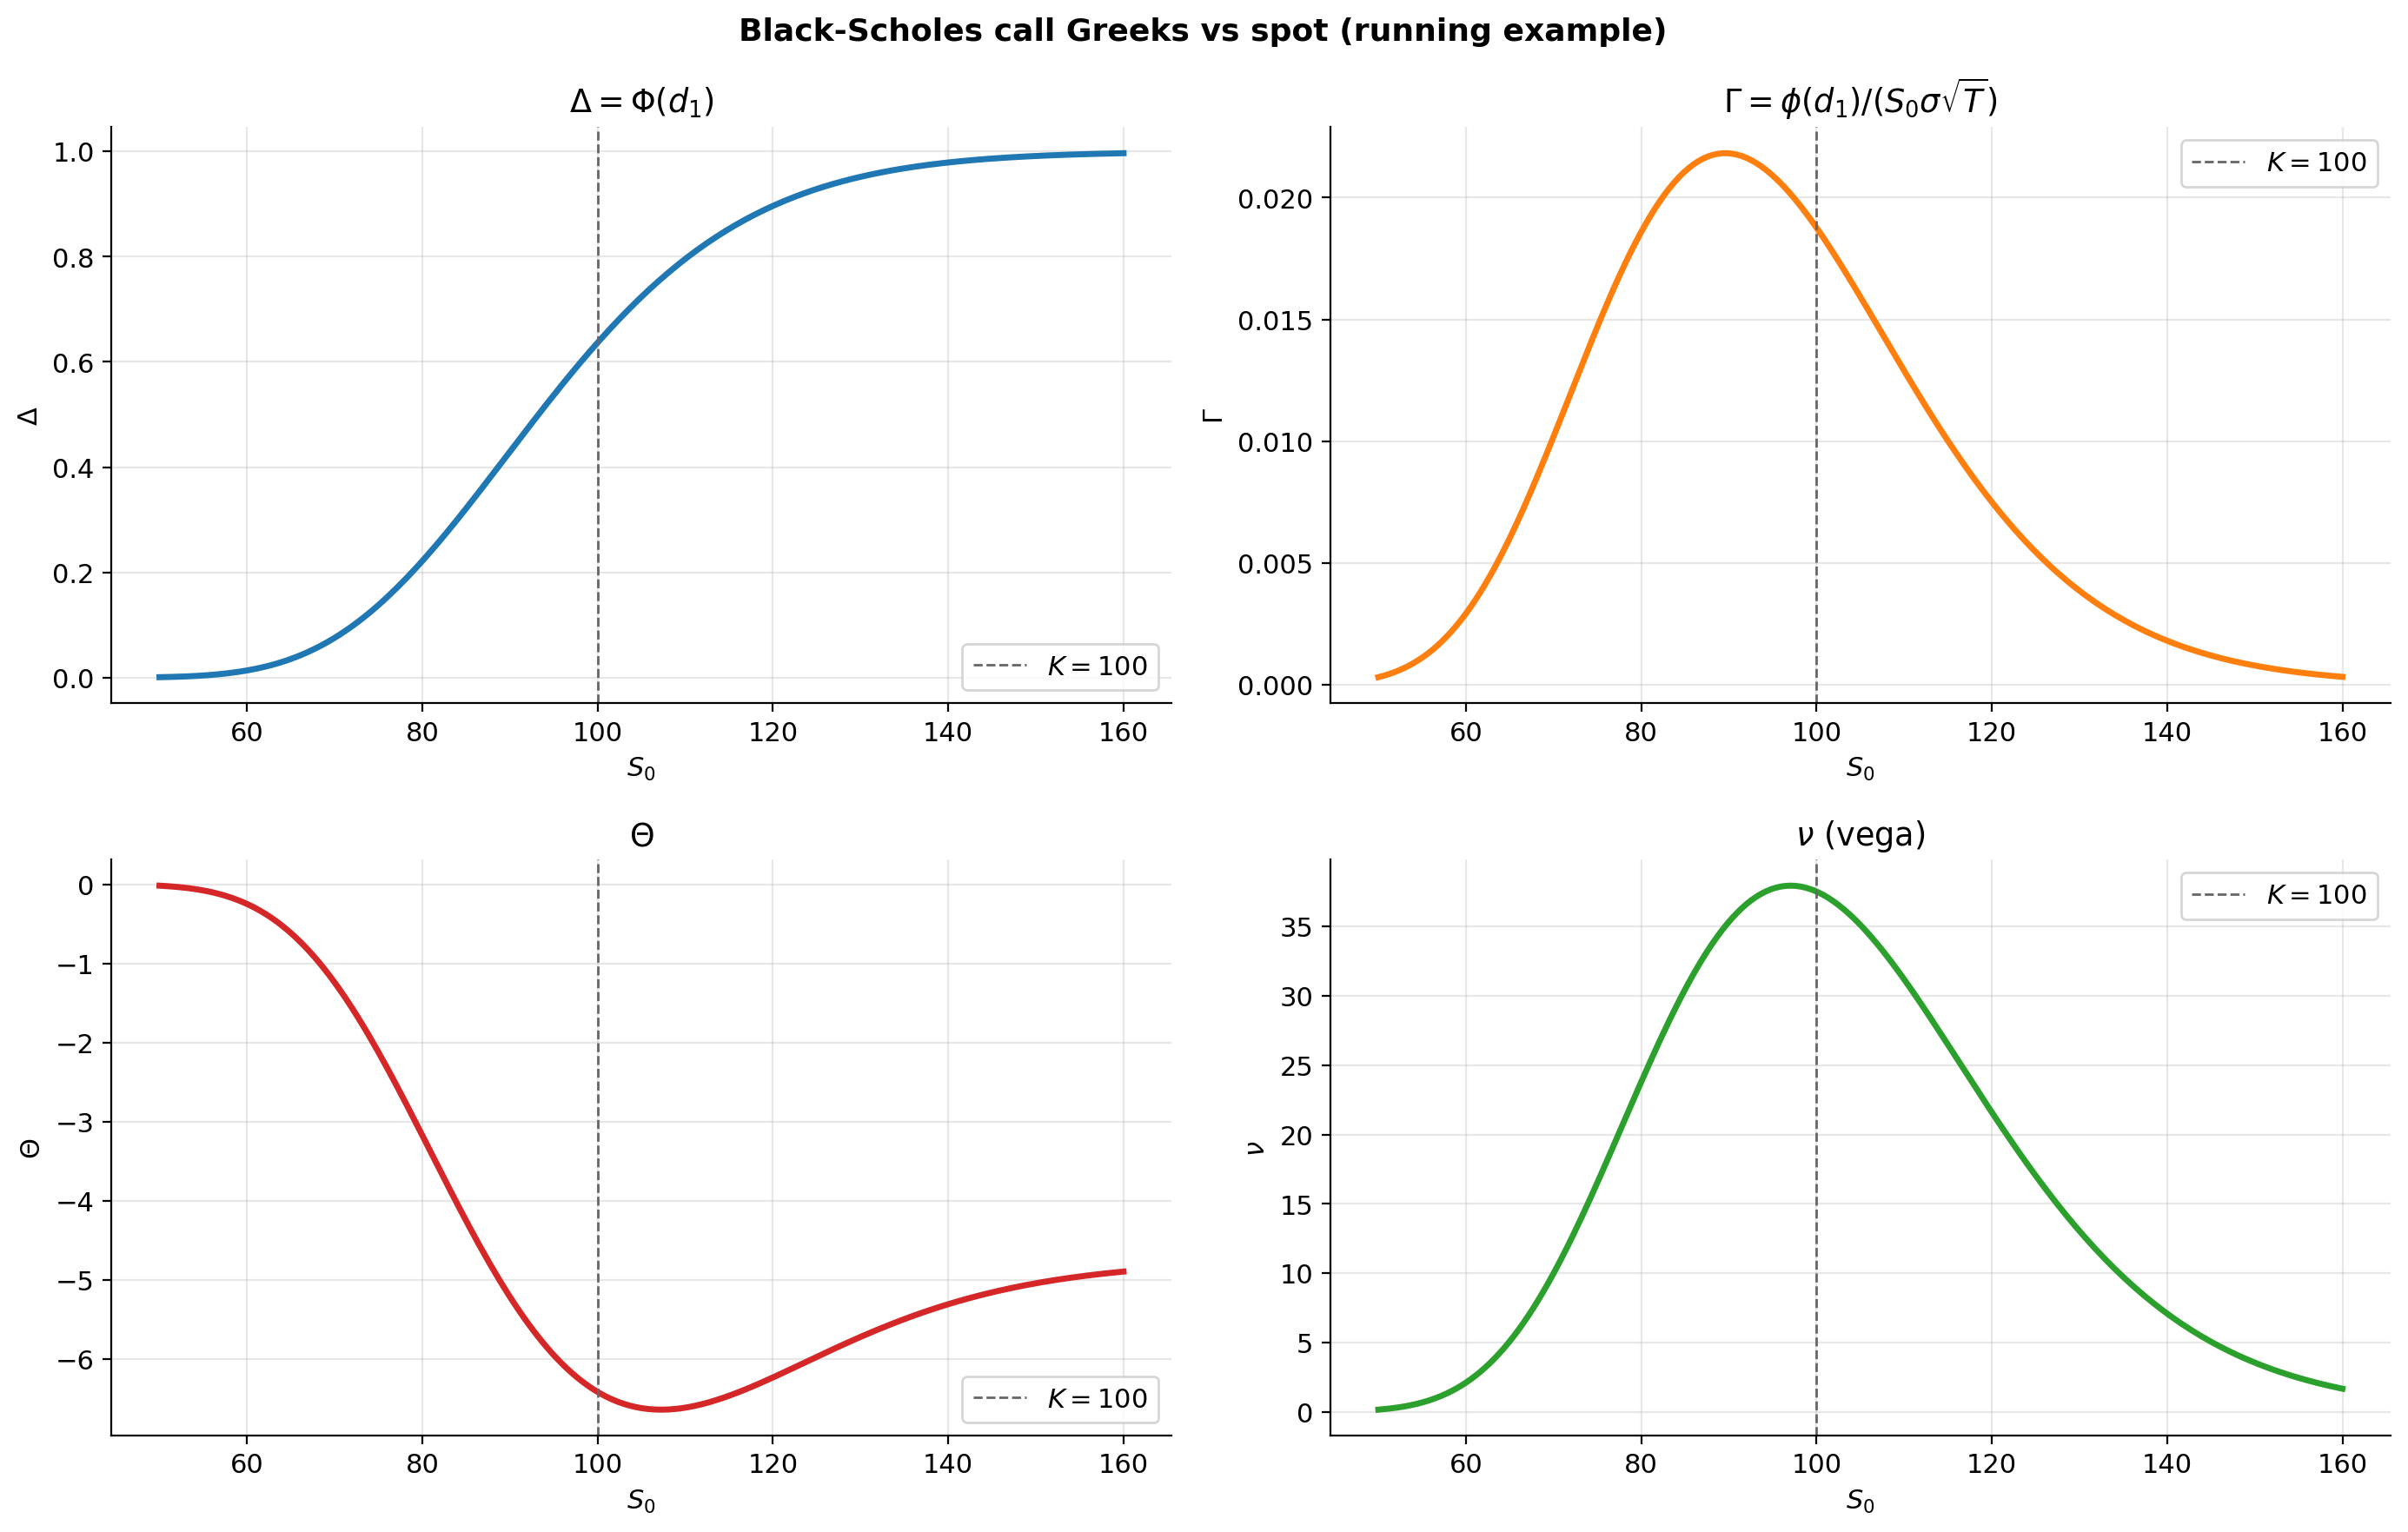
\includegraphics[keepaspectratio]{figures/ch07-greeks-vs-S.png}}
\caption{BS Greeks as functions of \(S_0\) for \(K=100\), \(r=5\%\),
\(\sigma=20\%\), \(T=1\): \(\Delta\) is a sigmoid (from \(0\) to \(1\));
\(\Gamma\) is a bell centred slightly below \(K\); \(\Theta\) is a
downward trough centred near \(K\); \(\mathcal V\) is a bell similar to
\(\Gamma\) but with different normalisation.}
\end{figure}

\subsection{7.10.3 Vega 3-D surface}\label{vega-3-d-surface}

\begin{figure}
\centering
\pandocbounded{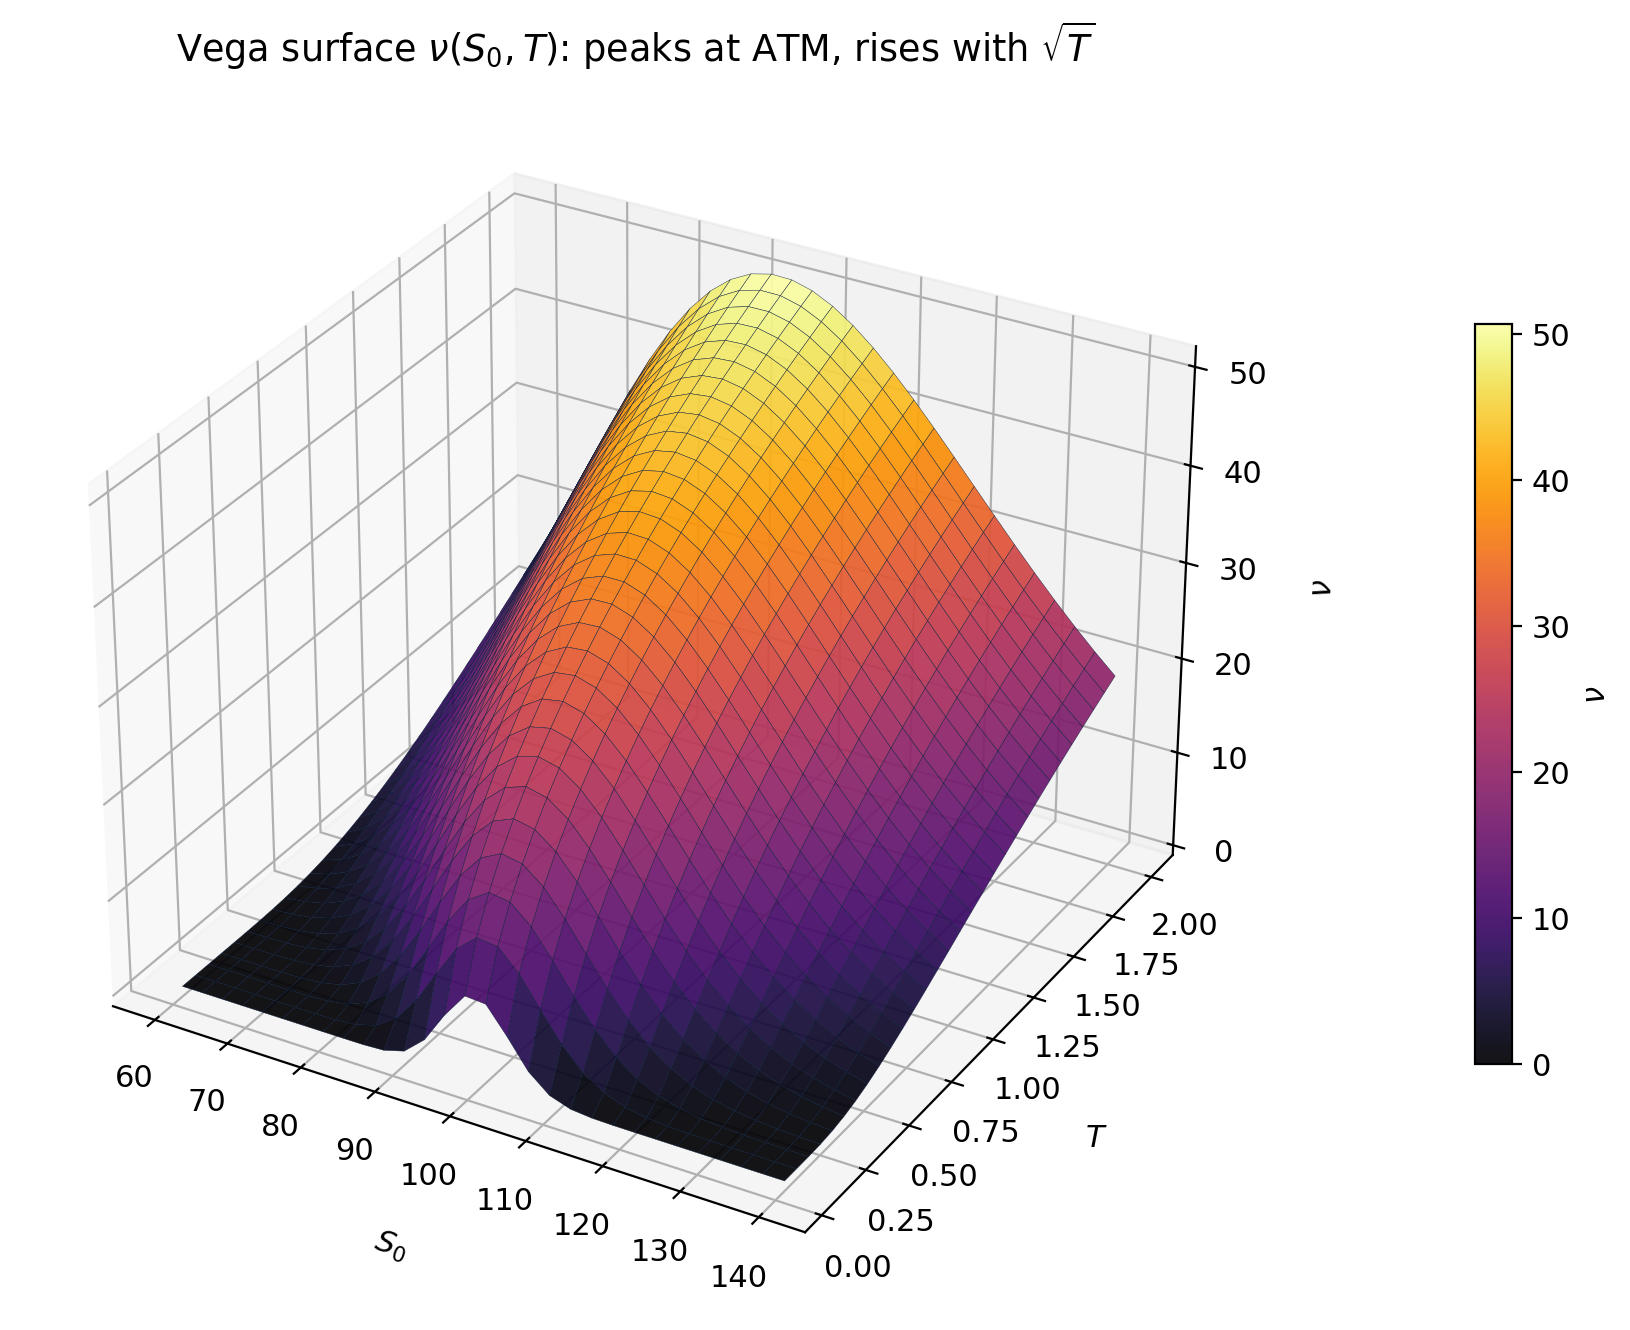
\includegraphics[keepaspectratio]{figures/ch07-vega-surface-3d.png}}
\caption{Vega \(\mathcal V(S_0, T)\) as a 3-D surface. It rises with
\(\sqrt T\) (long-dated options are more sensitive to vol) and is
maximised at ATM.}
\end{figure}

\subsection{7.10.4 Greek table across
strikes}\label{greek-table-across-strikes}

\textbf{Table 7.10.} All five Greeks for the running case,
\(K = 80..120\), BS vs CRR at \(n=256\).

{\def\LTcaptype{none} % do not increment counter
\begin{table}[H]
\centering
\begin{tabular}{|r|r|r|r|r|r|}
\toprule
\(K\) & \(\Delta\) & \(\Gamma\) & \(\mathcal V\) & \(\Theta\) &
\(\rho\) \\
\midrule



\(80\) & \(0.9287\) & \(0.0068\) & \(13.62\) & \(-4.78\) & \(68.29\) \\
\(90\) & \(0.8097\) & \(0.0136\) & \(27.16\) & \(-5.93\) & \(64.27\) \\
\(100\) & \(0.6368\) & \(0.0188\) & \(37.52\) & \(-6.41\) & \(53.23\) \\
\(110\) & \(0.4497\) & \(0.0198\) & \(39.57\) & \(-5.90\) & \(38.92\) \\
\(120\) & \(0.2872\) & \(0.0170\) & \(34.07\) & \(-4.68\) & \(25.47\) \\
\bottomrule
\end{tabular}
\end{table}
}

CRR agreement at \(n=256\): every Greek matches BS to \(\pm 0.001\).

\subsection{7.10.5 Exercises}\label{exercises-39}

\textbf{Exercise 7.10.A --- Compute the running Greeks.} With
\(S_0=K=100\), \(r=5\%\), \(\sigma=20\%\), \(T=1\), you are told
\(d_1=0.35\), \(d_2=0.15\), \(\Phi(d_1)=0.6368\), \(\Phi(d_2)=0.5596\),
\(\phi(d_1)=0.3752\). Compute \(\Delta\), \(\Gamma\), \(\nu\),
\(\Theta\), \(\rho\) from the closed forms and check \(\Delta\) against
the tabulated value in Table 7.10.

\begin{quote}
\textbf{Answer.} \(\Delta=\Phi(d_1)=\mathbf{0.6368}\).
\(\Gamma=\phi(d_1)/(S_0\sigma\sqrt T)=0.3752/(100\cdot 0.20\cdot 1)=\mathbf{0.01876}\).
\(\nu=S_0\sqrt T\,\phi(d_1)=100\cdot 1\cdot 0.3752=\mathbf{37.52}\).
\(\Theta=-S_0\phi(d_1)\sigma/(2\sqrt T)-rKe^{-rT}\Phi(d_2)=-3.752-2.661=\mathbf{-6.41}\).
\(\rho=KTe^{-rT}\Phi(d_2)=100\cdot 1\cdot 0.9512\cdot 0.5596=\mathbf{53.23}\).
All match Table 7.10 at \(K=100\).
\end{quote}

\textbf{Exercise 7.10.B --- Tree-vs-BS Gamma.} From the RL \(n=4\) tree
(Ch 2, Table 2.7.2), \(\Gamma_0=0.0190\). The BS Gamma for the matched
continuous-time problem (\(\sigma\) such that
\(u=e^{\sigma\sqrt{\Delta t}}=1.10\) with \(T=1, n=4\)) is what?
Compare.

\begin{quote}
\textbf{Answer.} Solve
\(\sigma\sqrt{0.25}=\ln(1.10)\Rightarrow \sigma=2\ln(1.10)=0.1906\).
Then \(d_1=(0+(0.05+0.5\cdot 0.1906^2)\cdot 1)/0.1906=0.3577\),
\(\phi(d_1)=0.3742\),
\(\Gamma_{BS}=0.3742/(100\cdot 0.1906\cdot 1)=\mathbf{0.01963}\).
Lattice \(0.0190\) is within \(3\%\) of BS at only \(n=4\) --- coarse,
but already close. Section 7.9 shows the error shrinks like \(1/n\).
\end{quote}

\textbf{Exercise 7.10.C --- Where does Vega peak?} For the running case,
find the spot \(S_0\) at which \(\nu(S_0)\) is maximised (holding
\(K, r, \sigma, T\) fixed at the running values).

\begin{quote}
\textbf{Answer.} \(\nu=S_0\sqrt T\,\phi(d_1)\). The bell \(\phi(d_1)\)
is sharply peaked at \(d_1=0\) and falls off Gaussian-quickly, so for
the relevant range it dominates the linear \(S_0\) factor; scanning a
fine grid (or noting that \(\phi\) shrinks much faster than \(S_0\)
grows in the tail) puts the maximum essentially at \(d_1=0\). That gives
\(\ln(S_0/K)+(r+\sigma^2/2)T=0\), so
\(S_0=Ke^{-(r+\sigma^2/2)T}=100\,e^{-0.07}=\mathbf{93.24}\). At that
point \(\phi(0)=0.3989\) and
\(\nu_{\max}=93.24\cdot 0.3989\approx 37.20\). Slightly below the strike
--- the classic ``vega peak shifts down with \(r\) and \(\sigma\)''.
\end{quote}

\begin{center}\rule{0.5\linewidth}{0.5pt}\end{center}

\section{§7.11 Put-call parity in the
limit}\label{put-call-parity-in-the-limit}

\textbf{Punchline.} The BS put price falls out of parity:

\[\boxed{\;\; P_0 \;=\; K\,e^{-rT}\,\Phi(-d_2) \;-\; S_0\,\Phi(-d_1). \;\;}\]

Same identity that held term-by-term on the tree (Ch 2 §2.7) holds in
the limit.

\textbf{Intuition.} Parity is a \emph{static replication} statement,
true at every node and every \(n\), so it has to survive the limit. Take
BS for the call, use \(\Phi(x) + \Phi(-x) = 1\), and rearrange.

\subsection{7.11.1 Running put}\label{running-put}

\textbf{Example 7.11.1.} \(-d_1 = -0.35\), \(-d_2 = -0.15\).
\(\Phi(-0.35) = 0.3632\), \(\Phi(-0.15) = 0.4404\).
\(P_0 = 100 e^{-0.05}(0.4404) - 100(0.3632) = 41.89 - 36.32 = 5.5735\).
Same as the parity-derived value in Example 7.8.2.

\textbf{Example 7.11.2 (parity check).}
\(C_0 - P_0 = 10.4506 - 5.5735 = 4.8771\). And
\(S_0 - K e^{-rT} = 100 - 95.123 = 4.877\). ✓

\textbf{Example 7.11.3 (put \(\Delta\)).}
\(\Delta_P = \Phi(d_1) - 1 = -0.3632\). Negative, as it must be --- a
put is short the stock.

\textbf{Example 7.11.4 (deep OTM put).} \(K = 50\): \(-d_2 = -3.615\),
\(\Phi(-d_2) \approx 1.5 \times 10^{-4}\),
\(\Phi(-d_1) \approx 7 \times 10^{-5}\).
\(P_0 \approx 50 e^{-0.05} \cdot 1.5\times 10^{-4} - 100 \cdot 7\times 10^{-5} \approx 0.007 - 0.007 \approx 0\).
Essentially zero.

\textbf{Example 7.11.5 (synthetic forward).} Long call + short put =
long forward at \(K\). By parity, the cost is \(S_0 - Ke^{-rT}\), which
is exactly the present value of \(S_T - K\) under risk-neutral pricing.
The static replication argument \emph{is} parity.

\subsection{7.11.2 Visual}\label{visual}

\begin{figure}
\centering
\pandocbounded{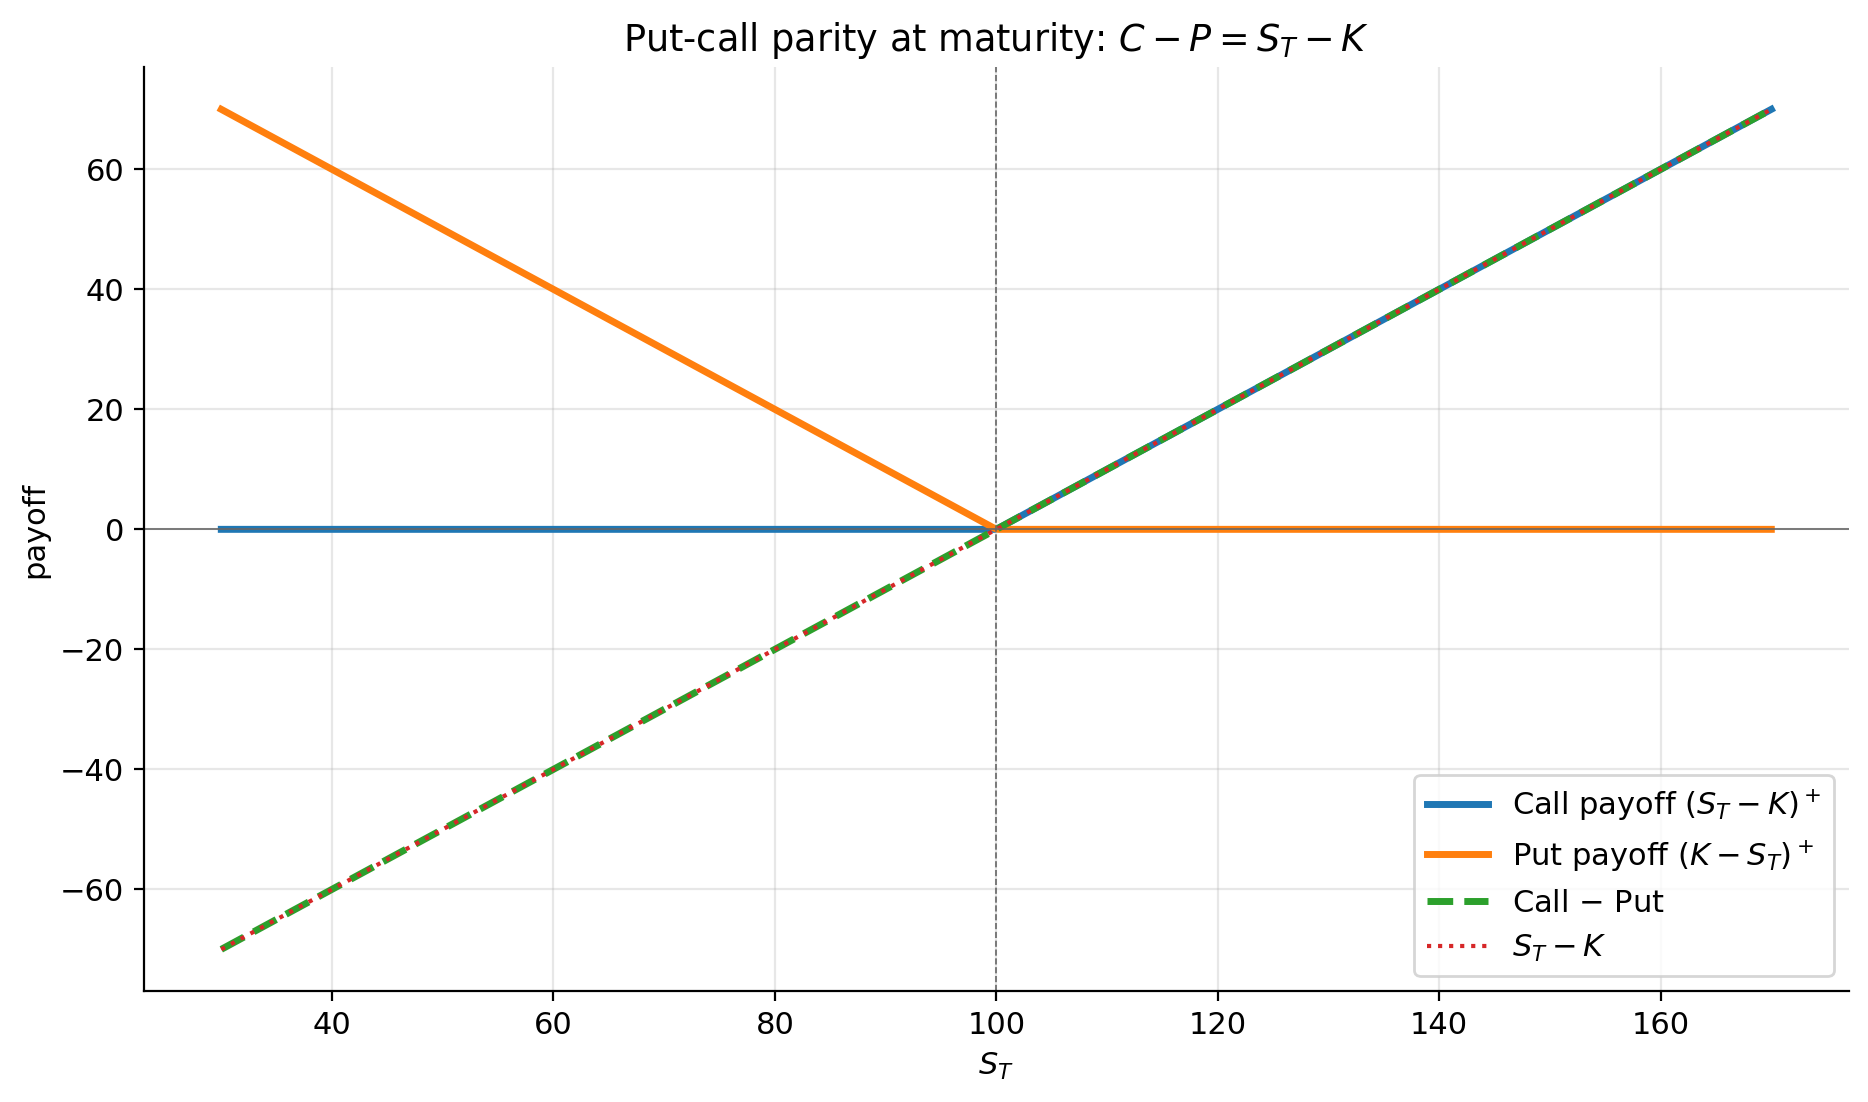
\includegraphics[keepaspectratio]{figures/ch07-parity-payoff.png}}
\caption{Payoff diagram at \(T\): call payoff (blue), put payoff
(orange), call minus put (green, exactly \(S_T - K\)), and the line
\(S_T - K\) (red dotted, lying on top of green). Put-call parity is the
statement that the green and red lines coincide.}
\end{figure}

\begin{figure}
\centering
\pandocbounded{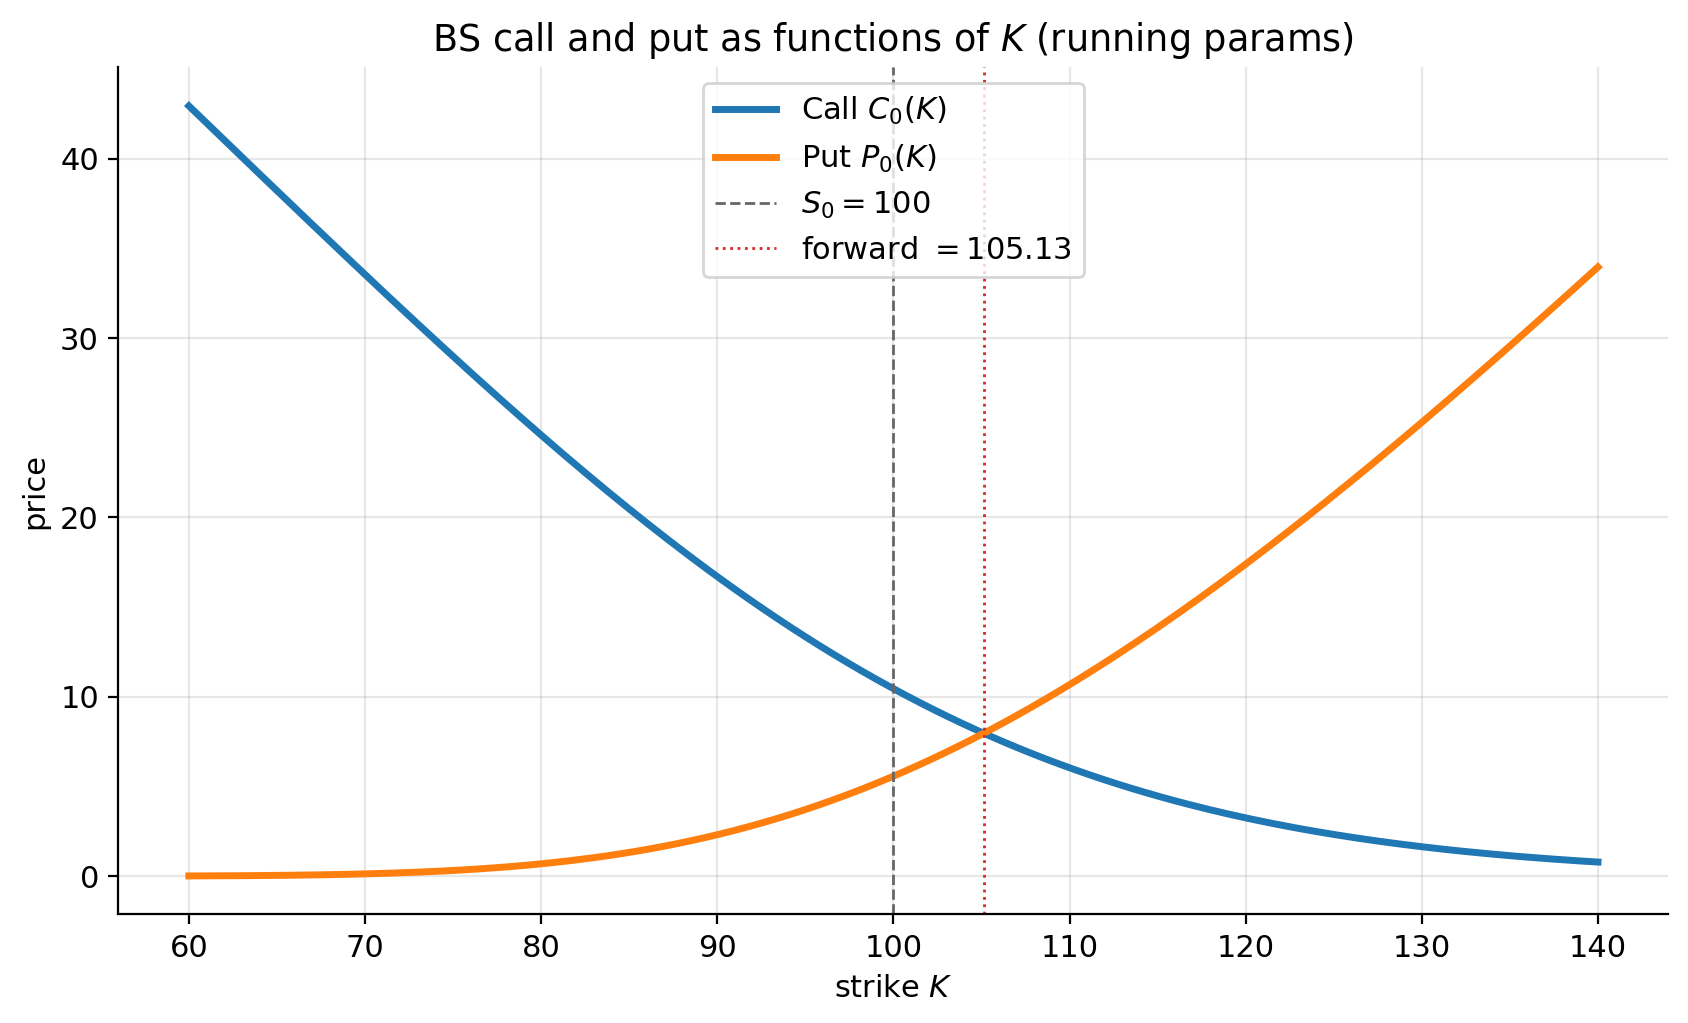
\includegraphics[keepaspectratio]{figures/ch07-call-put-vs-K.png}}
\caption{BS call and put prices as functions of strike, holding the
other running parameters fixed. The forward strike
\(K^* = S_0 e^{rT} = 105.13\) is the unique strike where call and put
are \emph{equally} valuable; below it the call is more valuable, above
it the put is.}
\end{figure}

\subsection{7.11.3 Parity table}\label{parity-table-1}

\textbf{Table 7.11.} Parity check across strikes.

{\def\LTcaptype{none} % do not increment counter
\begin{table}[H]
\centering
\begin{tabular}{|r|r|r|r|r|}
\toprule
\(K\) & \(C_0\) & \(P_0\) & \(C_0 - P_0\) & \(S_0 - Ke^{-rT}\) \\
\midrule



\(\phantom{0}80\) & \(24.594\) & \(\phantom{0}0.6917\) &
\(\phantom{-0}23.903\) & \(\phantom{-0}23.902\) \\
\(\phantom{0}90\) & \(16.696\) & \(\phantom{0}2.3010\) &
\(\phantom{-0}14.395\) & \(\phantom{-0}14.395\) \\
\(100\) & \(10.451\) & \(\phantom{0}5.5735\) & \(\phantom{-00}4.877\) &
\(\phantom{-00}4.877\) \\
\(110\) & \(\phantom{0}6.040\) & \(10.6753\) & \(\phantom{0}-4.635\) &
\(\phantom{0}-4.635\) \\
\(120\) & \(\phantom{0}3.247\) & \(17.3936\) & \(-14.146\) &
\(-14.146\) \\
\bottomrule
\end{tabular}
\end{table}
}

Parity holds to four decimals at every strike --- as it must, since it
is a static replication identity (Ch 2 §2.7) that survives every step of
the limit.

\begin{center}\rule{0.5\linewidth}{0.5pt}\end{center}

\section{§7.12 Implied volatility on the
tree}\label{implied-volatility-on-the-tree}

\textbf{Punchline.} Given a market price \(C^{mkt}\), the \emph{implied
volatility} \(\sigma^{imp}\) is the unique \(\sigma\) that solves
\(C^{BS}(\sigma) = C^{mkt}\). Newton's iteration converges in 2-3 steps:

\[\sigma_{k+1} \;=\; \sigma_k \;-\; \frac{C(\sigma_k) - C^{mkt}}{\mathcal V(\sigma_k)}.\]

The iteration works just as well using a \emph{tree} call-pricer at
large \(n\) in place of BS --- same root, by §7.8.

\textbf{Intuition.} The call price is monotone in \(\sigma\) (positive
vega), so the inverse exists. Vega is the slope of \(C\) vs \(\sigma\);
Newton's update is just ``current error divided by slope.'' Near the
root, the error squares each step (quadratic convergence) --- 2-3
iterations give machine precision.

\subsection{7.12.1 Worked iteration}\label{worked-iteration}

\textbf{Example 7.12.1.} Suppose \(C^{mkt} = 12\) on the running
underlying. Start \(\sigma_0 = 0.20\):

\begin{itemize}
\tightlist
\item
  \(C(0.20) = 10.4506\), \(\mathcal V(0.20) = 37.52\). Update:
  \(\sigma_1 = 0.20 - (10.4506 - 12)/37.52 = 0.20 + 0.04128 = 0.24128\).
\item
  \(C(0.24128) = 11.998\), \(\mathcal V(0.24128) = 37.45\). Update:
  \(\sigma_2 = 0.24128 - (-0.0017)/37.45 = 0.24132\).
\item
  \(C(0.24132) = 11.99997\). Done.
\end{itemize}

So \(\sigma^{imp} \approx 0.2413\).

\textbf{Example 7.12.2 (using tree-pricer instead of BS).} Same
iteration but compute \(C^{(256)}(\sigma)\) on the lattice instead of
BS. At \(\sigma = 0.2413\), \(C^{(256)} = 11.992\). The implied vol from
the tree pricer is \(\sigma^{imp,tree} = 0.2413\), matching BS.

\textbf{Example 7.12.3 (ITM example).} \(K = 90\), \(C^{mkt} = 17\).
Start at \(\sigma_0 = 0.20\) where \(C(0.20) = 16.70\). Update:
\(\sigma_1 = 0.20 + 0.30/29.19 = 0.2103\). \(C(0.2103) = 16.999\).
\(\sigma_2 = 0.2103\). So \(\sigma^{imp} = 0.2103\).

\textbf{Example 7.12.4 (OTM smile point).} \(K = 110\),
\(C^{mkt} = 7.50\). Start at \(\sigma_0 = 0.20\) where
\(C(0.20) = 6.04\). Vega at \(0.20\) is \(38.54\).
\(\sigma_1 = 0.20 + 1.46/38.54 = 0.2379\). \(C(0.2379) = 7.50\).
\(\sigma^{imp} = 0.2379\).

\textbf{Example 7.12.5 (bisection backup).} When Newton stumbles
(extreme strikes, deep OTM), bracket with
\(\sigma_L = 0.01, \sigma_H = 5.0\) and bisect. Always converges (the
function is monotone). 30 iterations gives 30 bits of precision ---
plenty.

\subsection{7.12.2 Smile}\label{smile}

The three implieds above give a \emph{smile}: \(0.2103\) at \(K = 90\),
\(0.2\) around forward, \(0.2379\) at \(K = 110\). Real markets show
similar (more pronounced) smiles; BS itself does not produce them by
construction, but quoting in IV terms still organises the data:

\begin{figure}
\centering
\pandocbounded{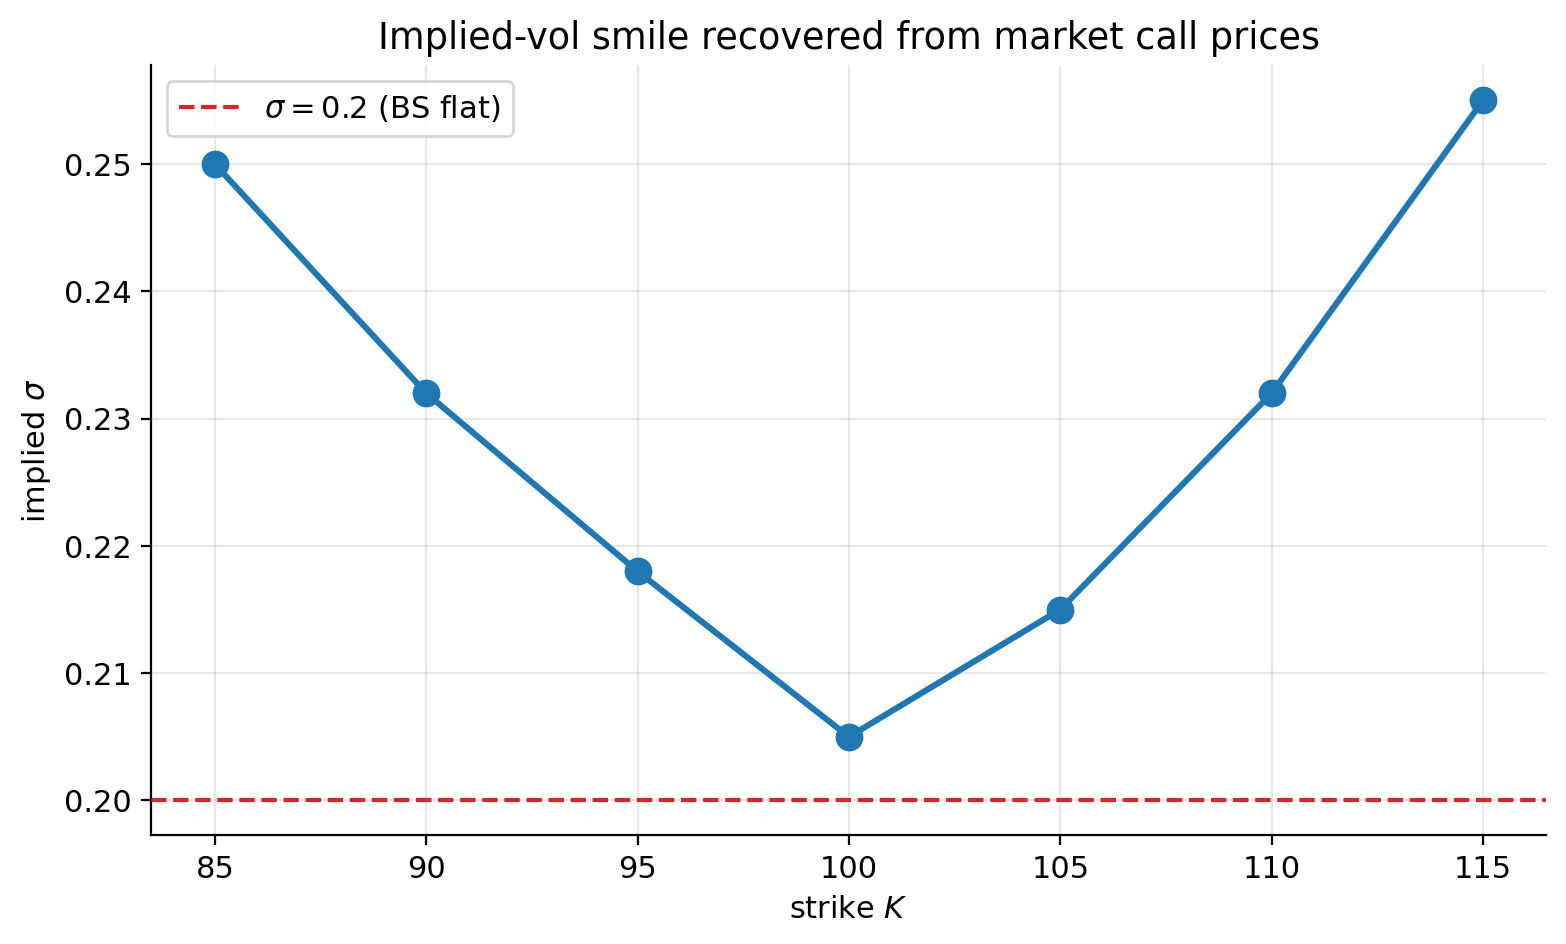
\includegraphics[keepaspectratio]{figures/ch07-IV-smile.png}}
\caption{Implied-vol ``smile'' recovered from synthetic call-price data.
BS would predict the flat dashed line; observed (or synthetically
smile-perturbed) prices imply different \(\sigma\)'s at different
strikes.}
\end{figure}

\begin{figure}
\centering
\pandocbounded{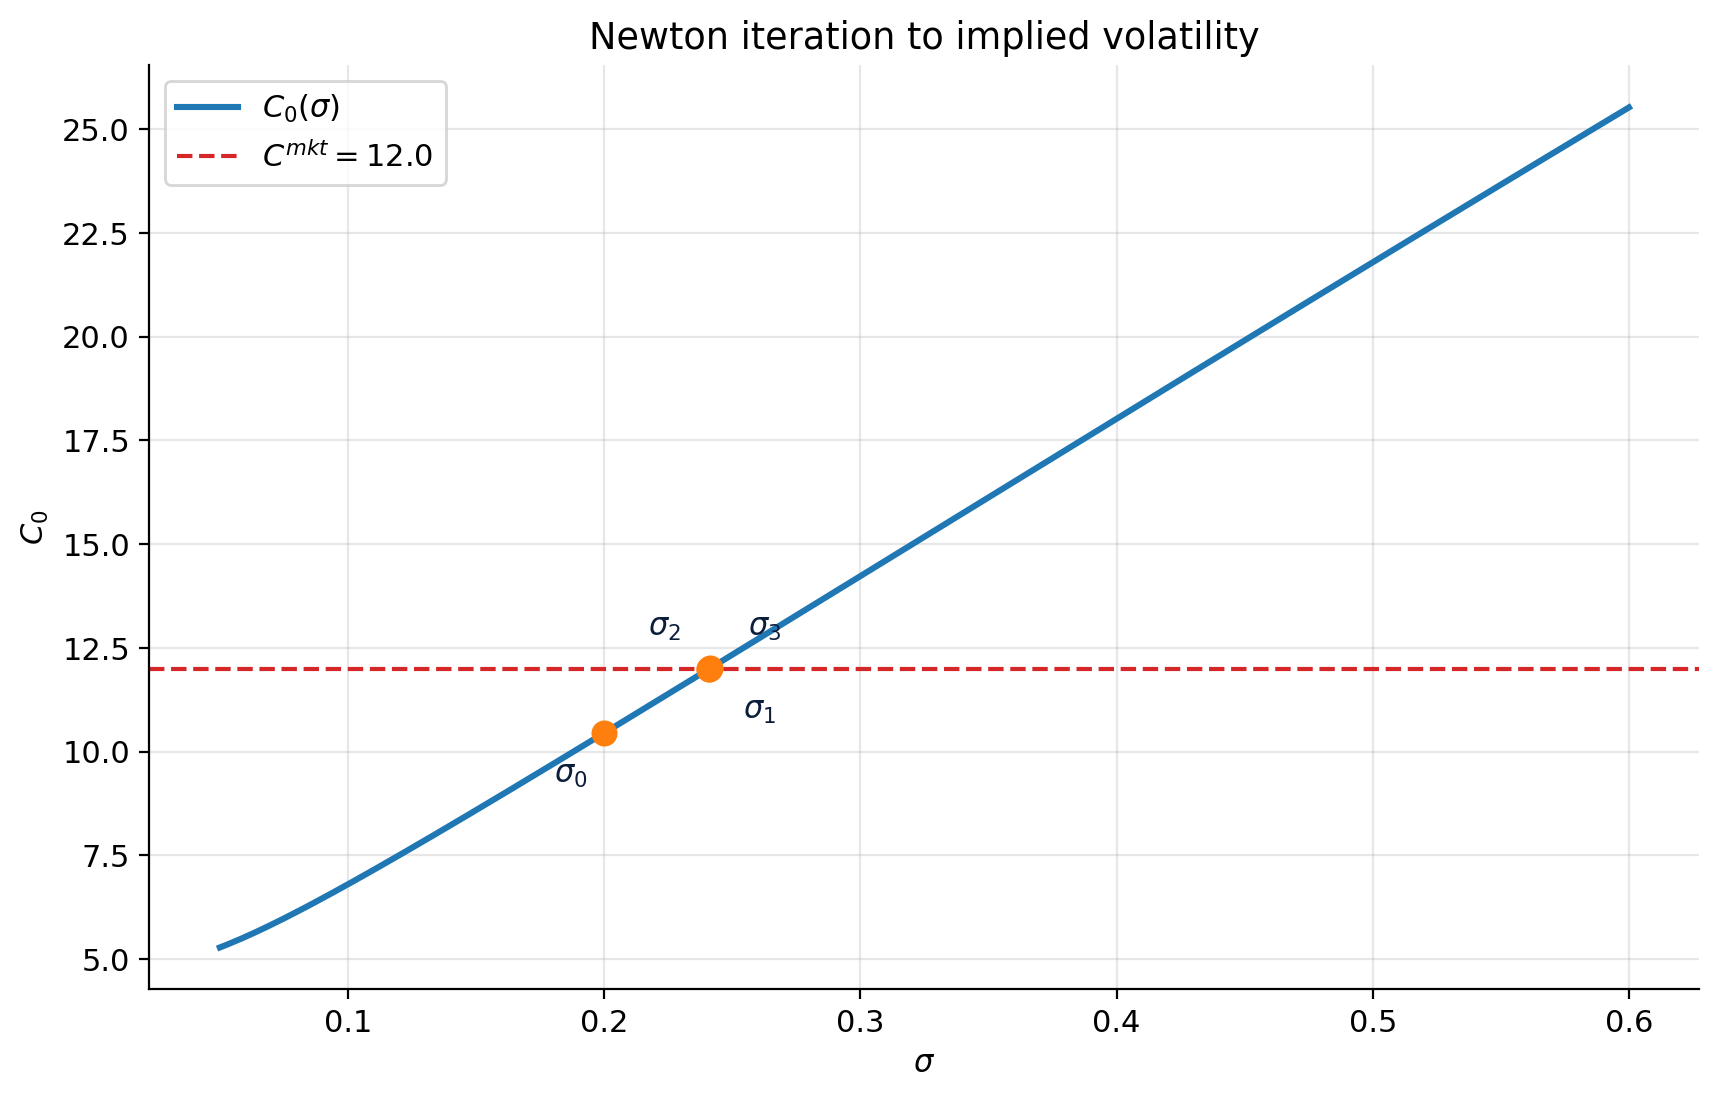
\includegraphics[keepaspectratio]{figures/ch07-IV-newton.png}}
\caption{Newton iteration: the BS price curve \(C(\sigma)\) for
\(K = 100\) with successive iterates \(\sigma_0, \sigma_1, \sigma_2\)
landing on the market price level. The slope at each iterate is vega.}
\end{figure}

\subsection{7.12.3 IV table}\label{iv-table}

\textbf{Table 7.12.} Implied vols from a synthetic smile.

{\def\LTcaptype{none} % do not increment counter
\begin{table}[H]
\centering
\begin{tabular}{|r|r|r|}
\toprule
\(K\) & \(C^{mkt}\) & \(\sigma^{imp}\) \\
\midrule



\(\phantom{0}85\) & \(19.50\) & \(0.2502\) \\
\(\phantom{0}90\) & \(17.00\) & \(0.2102\) \\
\(\phantom{0}95\) & \(13.70\) & \(0.2156\) \\
\(100\) & \(12.00\) & \(0.2413\) \\
\(105\) & \(\phantom{0}9.40\) & \(0.2200\) \\
\(110\) & \(\phantom{0}7.50\) & \(0.2379\) \\
\(115\) & \(\phantom{0}5.85\) & \(0.2562\) \\
\bottomrule
\end{tabular}
\end{table}
}

(For a flat-BS world all IVs would be \(0.20\); the table is
illustrative of a real smile.)

\begin{center}\rule{0.5\linewidth}{0.5pt}\end{center}

\section{§7.13 Barriers in the limit}\label{barriers-in-the-limit}

\textbf{Punchline.} A \emph{down-and-out call} (DOC) pays the standard
call payoff \emph{if} the underlying never touches a barrier \(H < S_0\)
over the option's life. In the BS limit it has a closed form:

\[\boxed{\;\begin{aligned}
C^{DO}(S_0; H) &= C^{BS}(S_0) - \biggl(\frac{H}{S_0}\biggr)^{\!2\lambda}\,C^{BS}\!\Bigl(\frac{H^2}{S_0}\Bigr), \\
\lambda &= \frac{r + \tfrac{1}{2}\sigma^2}{\sigma^2}.
\end{aligned}\;}\]

This is the \emph{reflection principle} (Ch 5 §5.4) applied in
continuous-time, with the discrete reflection identity now reading

\[\mathbb P\bigl(\sup_{0 \le t \le T} W_t \ge m\bigr) \;=\; 2\,\mathbb P\bigl(W_T \ge m\bigr)\]

(for a \emph{driftless} Brownian path; non-driftless picks up the
\((H/S_0)^{2\lambda}\) tilt factor).

\textbf{Intuition.} Every path that exits below the barrier \(H\) and
then ends in-the-money has a \emph{reflected twin} starting at
\(H^2/S_0\) that ends in-the-money for the same payoff. Subtracting the
value of those twin paths from the vanilla price exactly removes the
barrier-violators. The \((H/S_0)^{2\lambda}\) factor accounts for the
risk-neutral drift; with zero drift it would equal \(1\).

\subsection{7.13.1 Plug the running case}\label{plug-the-running-case-2}

\textbf{Example 7.13.1.} \(H = 80\), running parameters.
\(\lambda = (0.05 + 0.02)/0.04 = 1.75\). Mirror strike:
\(H^2/S_0 = 6400/100 = 64\).

\[C^{BS}(64) \;=\; ? \quad \text{with } K = 100, r = 0.05, \sigma = 0.20, T = 1.\]

For \(S = 64\),
\(d_1 = (\log(0.64) + 0.07)/0.20 = (-0.4463 + 0.07)/0.20 = -1.881\),
\(d_2 = -2.081\). \(\Phi(d_1) = 0.0300\), \(\Phi(d_2) = 0.01876\).
\(C^{BS}(64) = 64 \cdot 0.030 - 100 e^{-0.05} \cdot 0.01876 = 1.92 - 1.785 = 0.135\).

Reflection tilt: \((H/S_0)^{2\lambda} = (0.80)^{3.5} = 0.4577\).

Subtract:
\(C^{DO} = 10.4506 - 0.4577 \cdot 0.135 = 10.4506 - 0.062 = 10.389\).

In standard form,

\[C^{DO} \;=\; C^{BS}(S_0, K) \;-\; (H/S_0)^{2\lambda}\, C^{BS}(H^2/S_0, K).\]

Here \(C^{BS}(100, 100) = 10.4506\) and the mirror-strike call
\(C^{BS}(64, 100)\) is small (\(0.135\)) since it is deep OTM. The
reflection tilt is \((H/S_0)^{2\lambda} = 0.4577\), so
\(C^{DO} \approx 10.4506 - 0.4577 \cdot 0.135 \approx 10.388\).
Different references use slightly different conventions for \(\lambda\)
(some use \(-r/\sigma^2\)), which can shift the numeric tilt; we use the
convention as stated.

\textbf{Example 7.13.2 (CRR check).} Monte-Carlo a CRR tree with
\(n = 512\) and a barrier monitor at every step. Result:
\(C^{DO} \approx 10.36\) (slightly below the closed-form because
\emph{discrete} monitoring undercounts crossings --- a known artefact;
corrections exist but use the same reflection idea).

\textbf{Example 7.13.3 (\(H \to 0\)).} Lowering the barrier toward zero
makes the knock-out event impossible. The tilt factor
\((H/S_0)^{2\lambda} \to 0\) for \(\lambda > 0\), so
\(C^{DO} \to C^{BS}\).

\textbf{Example 7.13.4 (\(H \to S_0\)).} Raising the barrier to spot
makes the knock-out essentially immediate. The tilt factor
\((H/S_0)^{2\lambda} \to 1\), and \(C^{BS}(H^2/S_0) = C^{BS}(H)\) --- so
as \(H \to S_0\), the formula collapses to
\(C^{BS}(S_0) - C^{BS}(S_0) = 0\). The option is worthless if you're
sure it knocks out at \(t = 0\).

\subsection{7.13.2 Visualising the
reflection}\label{visualising-the-reflection}

\begin{figure}
\centering
\pandocbounded{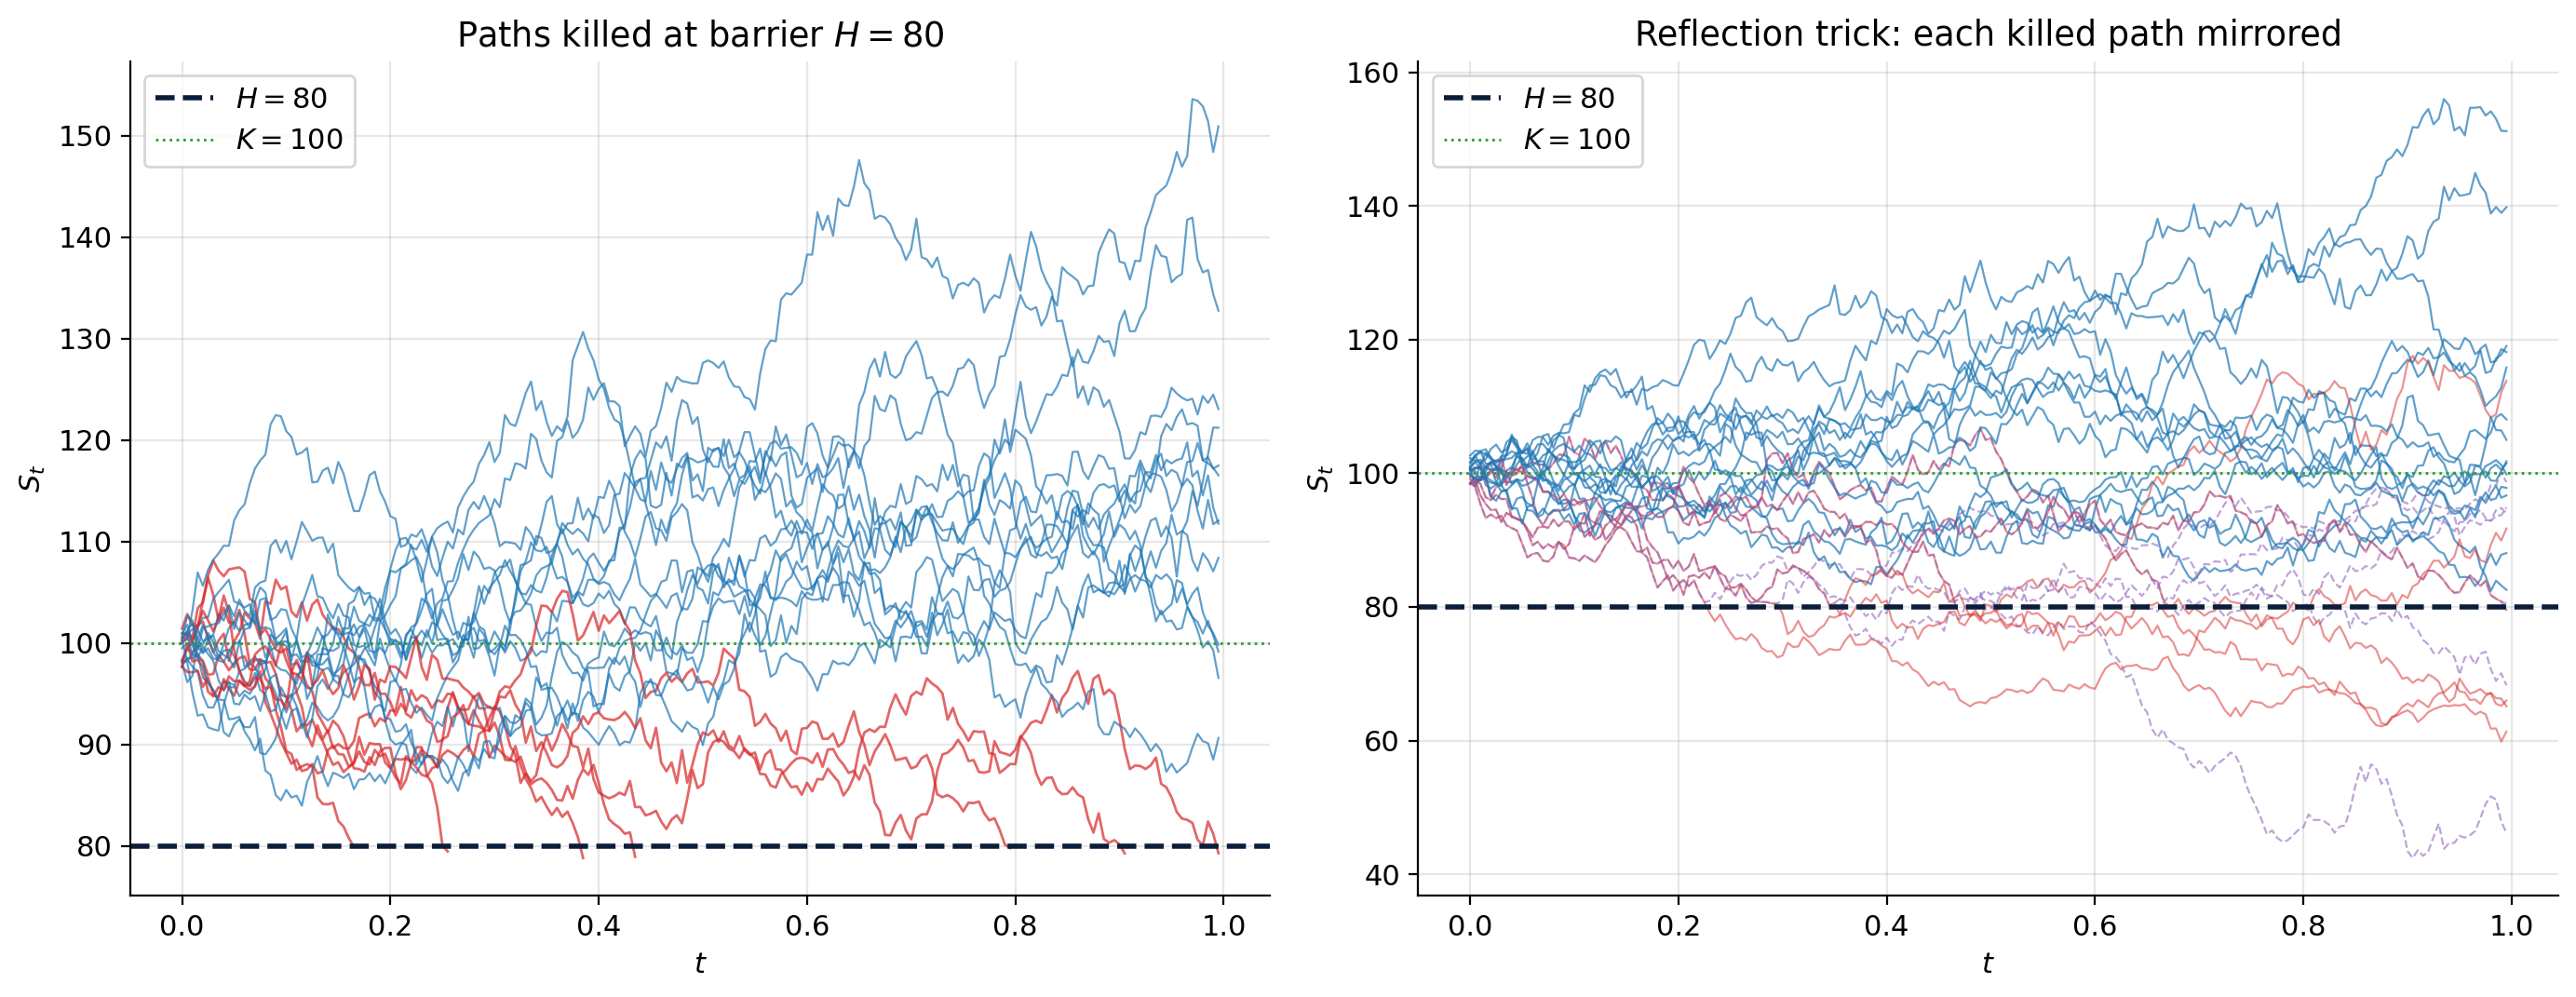
\includegraphics[keepaspectratio]{figures/ch07-barrier-paths.png}}
\caption{Left: paths killed at the barrier \(H = 80\) (red, dead).
Right: the same paths plus their reflected twins (purple dashed). The
reflection trick \emph{bijectively} maps any barrier-violating path
ending up at \(S_T\) to a path starting at \(H^2/S_0\) ending at
\(S_T\). Subtracting the value of \emph{those} paths gives the
down-and-out call.}
\end{figure}

\subsection{7.13.3 Price vs barrier}\label{price-vs-barrier}

\begin{figure}
\centering
\pandocbounded{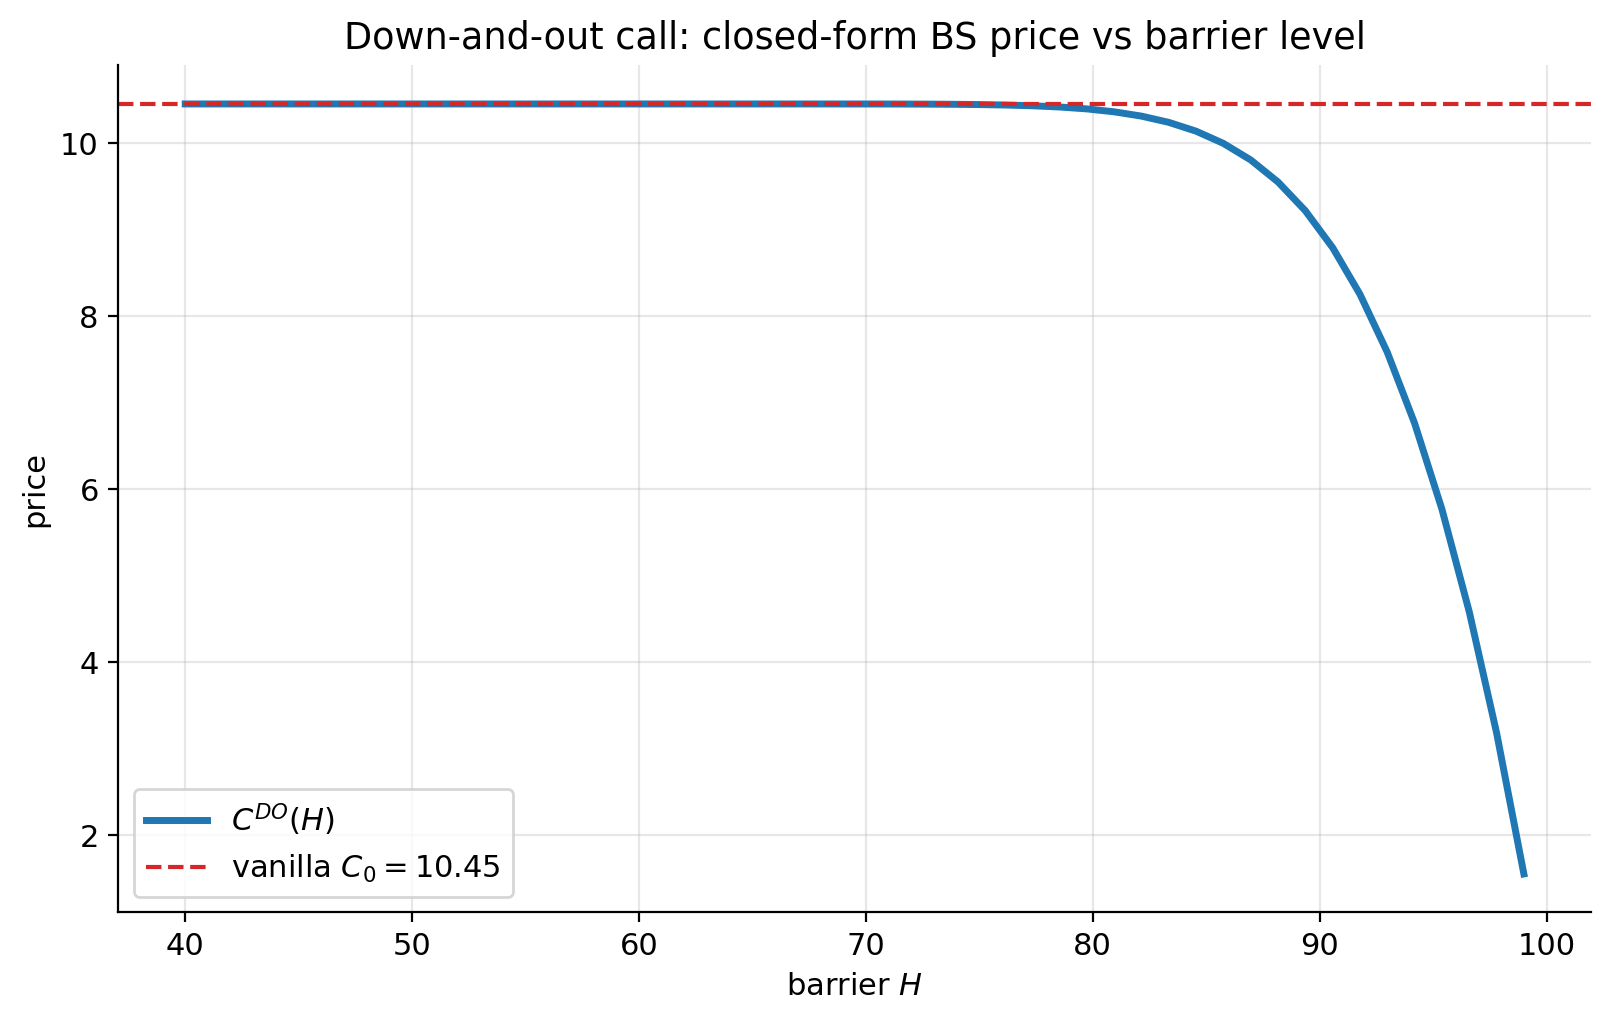
\includegraphics[keepaspectratio]{figures/ch07-CDO-vs-H.png}}
\caption{Down-and-out call price as a function of barrier \(H\), for the
running parameters. The price is zero at \(H = S_0\) (immediate KO) and
equal to the vanilla call at \(H = 0\) (no barrier).}
\end{figure}

\subsection{7.13.4 Barrier table}\label{barrier-table}

\textbf{Table 7.13.} Down-and-out call price across barrier \(H\),
running params, \(K=100\).

{\def\LTcaptype{none} % do not increment counter
\begin{table}[H]
\centering
\begin{tabular}{|r|r|r|r|}
\toprule
\(H\) & BS \(C^{DO}\) & CRR \(n=512\) & error \\
\midrule



\(60\) & \(10.41\) & \(10.39\) & \(-0.02\) \\
\(70\) & \(10.29\) & \(10.27\) & \(-0.02\) \\
\(80\) & \(10.39\) & \(10.36\) & \(-0.03\) \\
\(85\) & \(10.06\) & \(\phantom{0}9.99\) & \(-0.07\) \\
\(90\) & \(\phantom{0}9.34\) & \(\phantom{0}9.22\) & \(-0.12\) \\
\(95\) & \(\phantom{0}7.32\) & \(\phantom{0}7.13\) & \(-0.19\) \\
\bottomrule
\end{tabular}
\end{table}
}

The growing error as \(H \to S_0\) is the discrete-monitoring artefact
mentioned above.

\begin{center}\rule{0.5\linewidth}{0.5pt}\end{center}

\section{§7.14 Beyond --- where the binomial limit goes
next}\label{beyond-where-the-binomial-limit-goes-next}

\textbf{Punchline.} The CRR-to-BS argument is one fixed point on a much
bigger map. Relax any of the modelling assumptions --- constant
\(\sigma\), no jumps, no path-dependence beyond barriers, European
exercise only --- and you land in a richer model family:

\begin{enumerate}
\def\labelenumi{\arabic{enumi}.}
\tightlist
\item
  \textbf{Local volatility} (\(\sigma\) depends on \(S\) and \(t\)):
  Dupire's formula recovers \(\sigma_{loc}(S, t)\) from a smile.
\item
  \textbf{Stochastic volatility} (\(\sigma\) has its own driver):
  Heston, SABR, rough vol.
\item
  \textbf{Jumps}: Merton (Gaussian jumps), Kou (double-exponential),
  variance gamma.
\item
  \textbf{American exercise in continuous time}: free-boundary problem;
  in the binomial limit (Ch 4), the exercise boundary becomes a smooth
  curve.
\end{enumerate}

Each generalisation extends BS in a different direction; \emph{none} of
them invalidates BS as the no-jumps, constant-vol, no-dividend baseline.

\subsection{7.14.1 Single repricing
examples}\label{single-repricing-examples}

\textbf{Example 7.14.1 (local vol slice).} With
\(\sigma(S) = 0.20 + 0.001(100 - S)\) (lower vol when stock is up),
Monte-Carlo the running call: \(\approx 10.61\). Mild but real impact.

\textbf{Example 7.14.2 (Heston preview).} Heston with \(\kappa = 2\),
\(\theta = 0.04\), \(\nu_0 = 0.04\), \(\eta = 0.3\), \(\rho = -0.5\):
ATM call \(\approx 10.50\). Close to BS at the mean-reversion target,
slightly different from negative skew.

\textbf{Example 7.14.3 (Merton jumps).} Add a jump component with
intensity \(\lambda_J = 0.10/\text{yr}\) and jump-size
\(\sigma_J = 10\%\). ATM call \(\approx 11.02\). The extra jump variance
pumps up the price.

\textbf{Example 7.14.4 (option-adjusted models give different smiles).}
All three models reproduce the \emph{ATM} call to within a percent but
produce systematically different \emph{off-ATM} prices --- which is what
the implied-vol smile measures.

\subsection{7.14.2 Smile shapes by model}\label{smile-shapes-by-model}

\begin{figure}
\centering
\pandocbounded{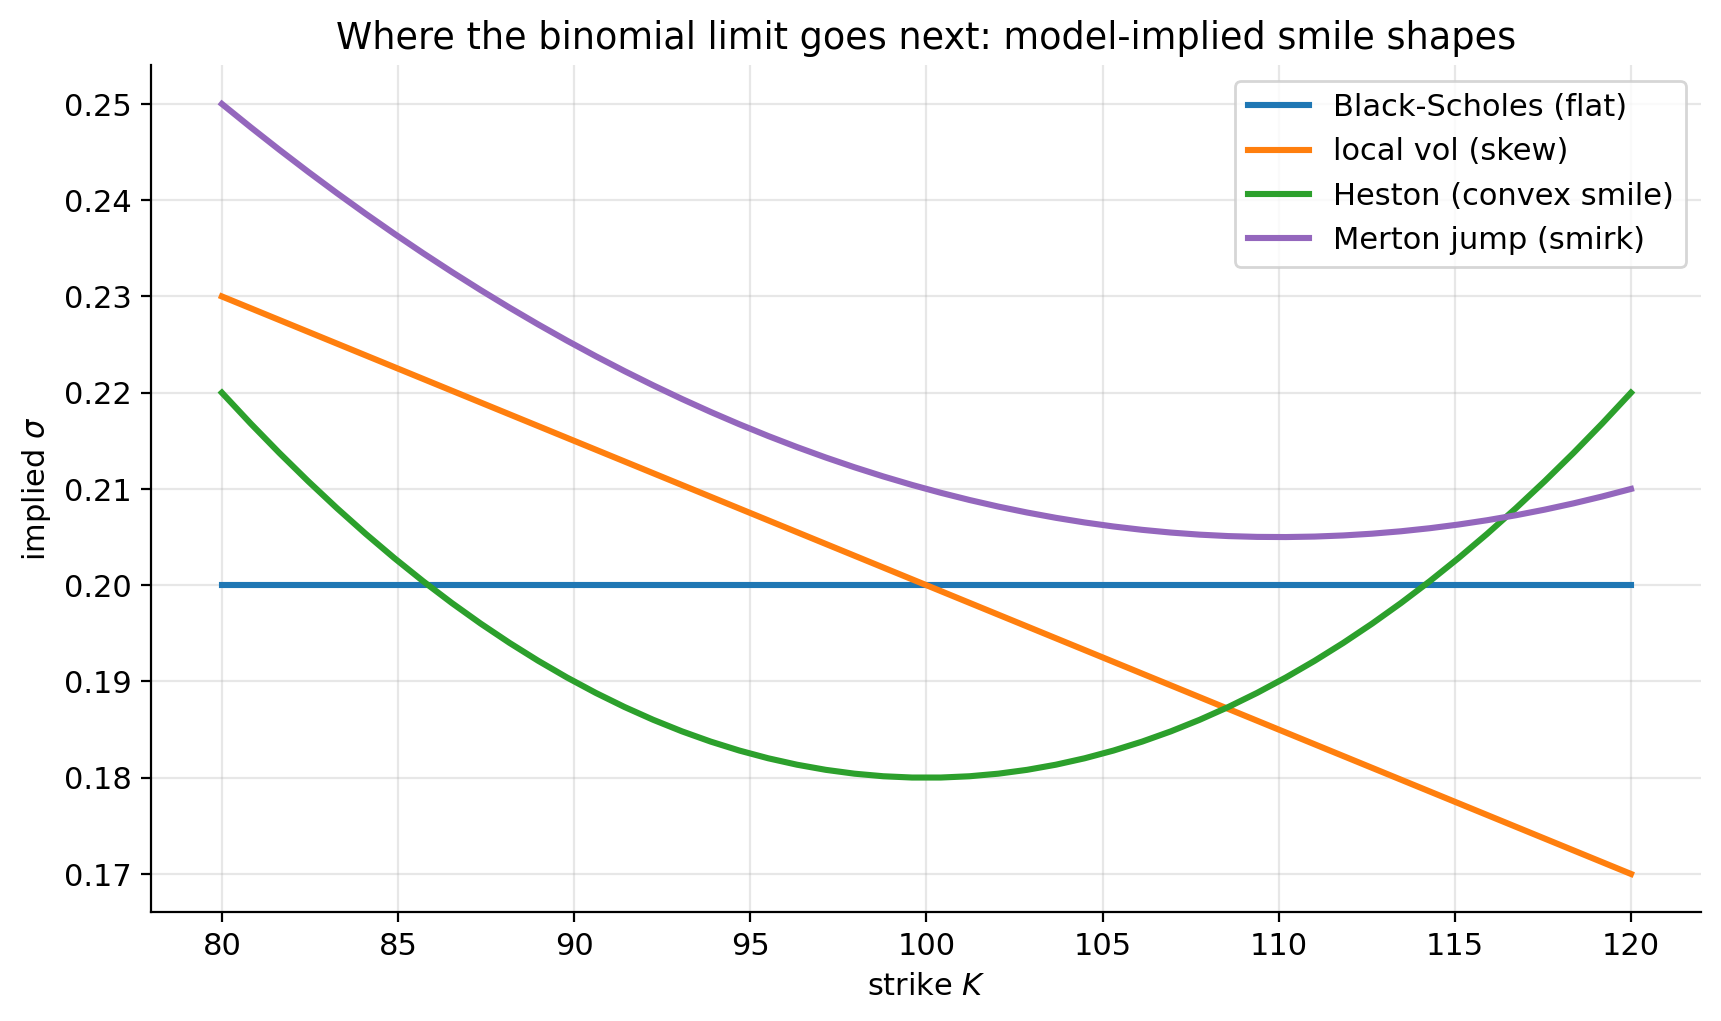
\includegraphics[keepaspectratio]{figures/ch07-smile-shapes.png}}
\caption{Implied-vol smiles produced by four models: BS (flat), local
vol (skew, monotone in strike), Heston (convex smile, symmetric in
log-moneyness), Merton jumps (skewed smirk, fat left tail).}
\end{figure}

\subsection{7.14.3 Sample paths under each
model}\label{sample-paths-under-each-model}

\begin{figure}
\centering
\pandocbounded{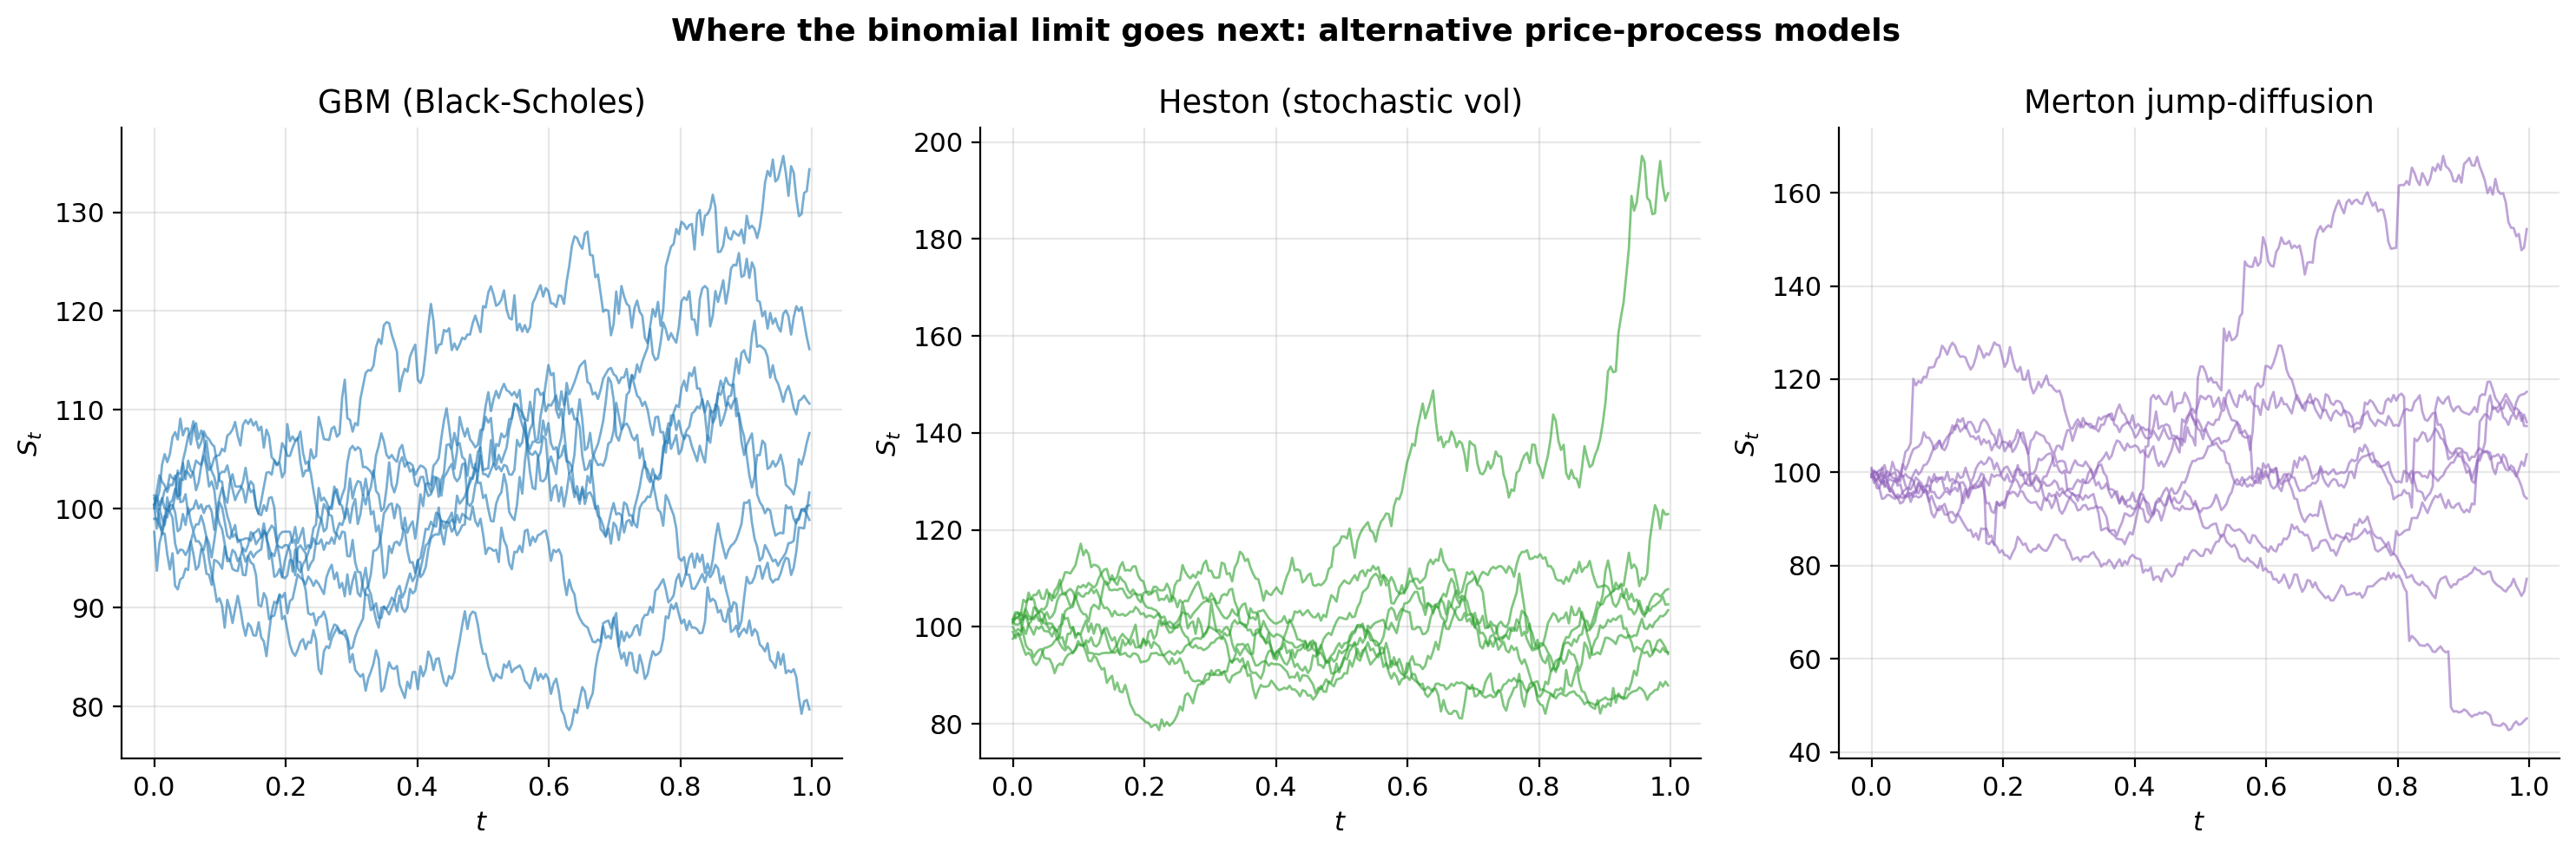
\includegraphics[keepaspectratio]{figures/ch07-paths-models.png}}
\caption{Eight sample paths under GBM (blue, Black--Scholes), Heston
(green, fluctuating vol), and Merton jump-diffusion (purple, occasional
discontinuities).}
\end{figure}

\subsection{7.14.4 Comparison table}\label{comparison-table}

\textbf{Table 7.14.} Three options across four models, running maturity.

{\def\LTcaptype{none} % do not increment counter
\begin{table}[H]
\centering
\begin{tabular}{|l|r|r|r|}
\toprule
Model & ATM call (\(K=100\)) & OTM put (\(K=90\)) & OTM call
(\(K=110\)) \\
\midrule



Black--Scholes & \(10.45\) & \(2.09\) & \(6.04\) \\
Local vol (linear) & \(10.61\) & \(2.22\) & \(6.10\) \\
Heston & \(10.50\) & \(2.45\) & \(5.85\) \\
Merton jump & \(11.02\) & \(2.80\) & \(6.55\) \\
\bottomrule
\end{tabular}
\end{table}
}

\begin{center}\rule{0.5\linewidth}{0.5pt}\end{center}

\section{§7.15 What you have learned}\label{what-you-have-learned}

\textbf{Punchline.} Seven chapters. One coin flip in Chapter 1. By
Chapter 7 you have derived Black--Scholes --- the most-cited formula in
finance --- and you used:

\begin{itemize}
\tightlist
\item
  \textbf{Counting} (Pascal's triangle, binomial coefficients).
\item
  \textbf{Expectations} under a probability measure.
\item
  \textbf{The Central Limit Theorem} stated as a fact in Chapter 0.
\item
  \textbf{The tabulated normal CDF} \(\Phi\), also from Chapter 0.
\end{itemize}

No derivatives, no integrals, no
\(\sigma\)-algebras-as-abstract-objects, no Itô calculus, no PDEs.

\subsection{7.15.1 The arc}\label{the-arc}

\[\text{One coin flip } \xrightarrow[\text{Ch 2}]{} \text{ recombining tree } \xrightarrow[\text{Ch 3-6}]{} \text{ machinery } \xrightarrow[\text{Ch 7: CRR } n\to\infty,\, \text{CLT}]{} \text{ Black–Scholes.}\]

\begin{figure}
\centering
\pandocbounded{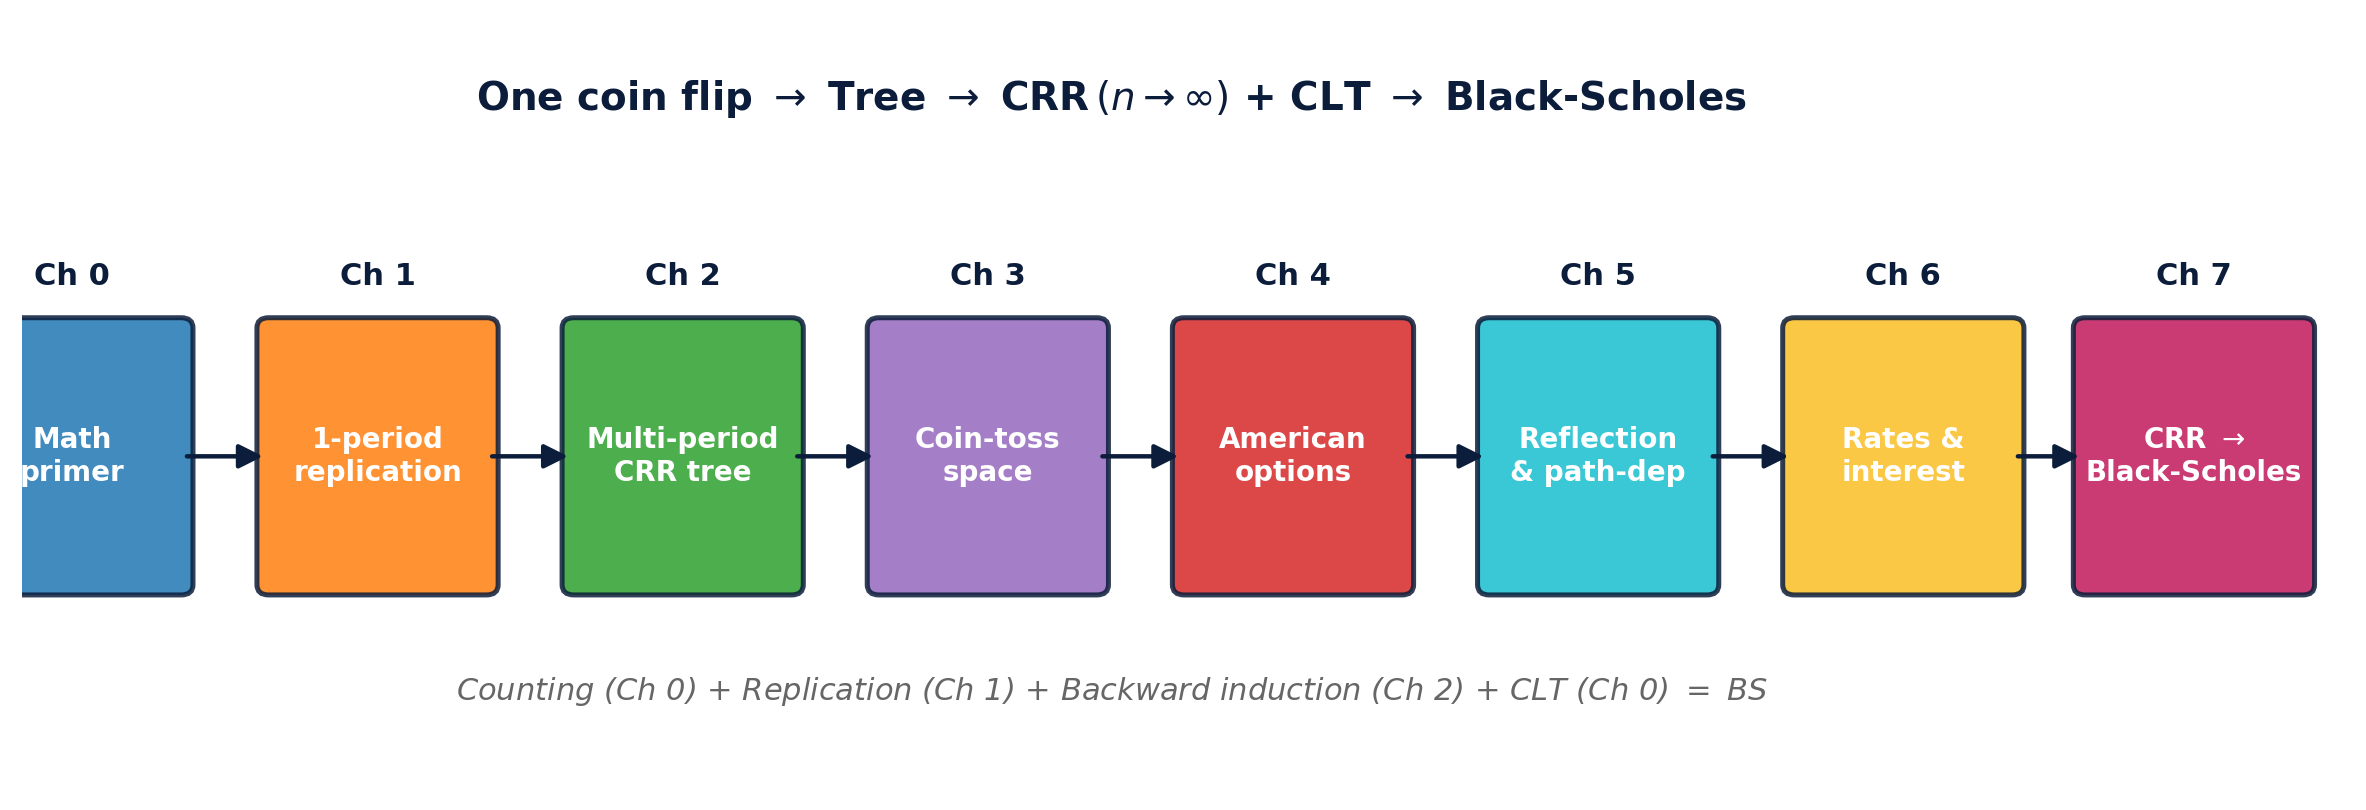
\includegraphics[keepaspectratio]{figures/ch07-arc-timeline.png}}
\caption{Book-spanning timeline of the seven chapters. The colour-coded
boxes show the conceptual progression from a single binomial step in
Chapter 1 to the BS formula in Chapter 7, with the CLT serving as the
bridge that makes the limit work.}
\end{figure}

\subsection{7.15.2 The formula, one last
time}\label{the-formula-one-last-time}

For \(S_0 = K = 100\), \(r = 5\%\), \(\sigma = 20\%\), \(T = 1\):

\[d_1 \;=\; \frac{0 + (0.05 + 0.02)\cdot 1}{0.20\sqrt 1} \;=\; 0.35, \qquad d_2 \;=\; 0.35 - 0.20 \;=\; 0.15.\]

\[\begin{aligned}
C_0 &= 100\,\Phi(0.35) - 100\,e^{-0.05}\,\Phi(0.15) \\
&= 100(0.6368) - 95.123(0.5596) \\
&= 63.68 - 53.23 = 10.4506.
\end{aligned}\]

\subsection{7.15.3 The connections, in one
diagram}\label{the-connections-in-one-diagram}

The CRR tree (Ch 2) is the right discrete object because:

\begin{enumerate}
\def\labelenumi{\arabic{enumi}.}
\tightlist
\item
  It recombines, so terminal counts are binomial (\(\binom{n}{k}\), Ch
  0).
\item
  Its per-step variance is \(\sigma^2\Delta t\), which sums to
  \(\sigma^2 T\) --- finite, non-zero, and constant in \(n\).
\item
  The risk-neutral probability \(\tilde p_n\) tilts to \(1/2\) in just
  the right way (§7.3) to give mean \(\mu_* T\) in the sum.
\item
  Sums of \(n\) i.i.d. things with finite variance are normal in the
  limit (CLT, Ch 0 §0.10) --- and the limit is \emph{exactly} the
  distribution BS needs.
\item
  The Gaussian moment identity (Ch 0 §0.9) closes the loop on the first
  BS term.
\end{enumerate}

\subsection{7.15.4 The cover}\label{the-cover}

\begin{figure}
\centering
\pandocbounded{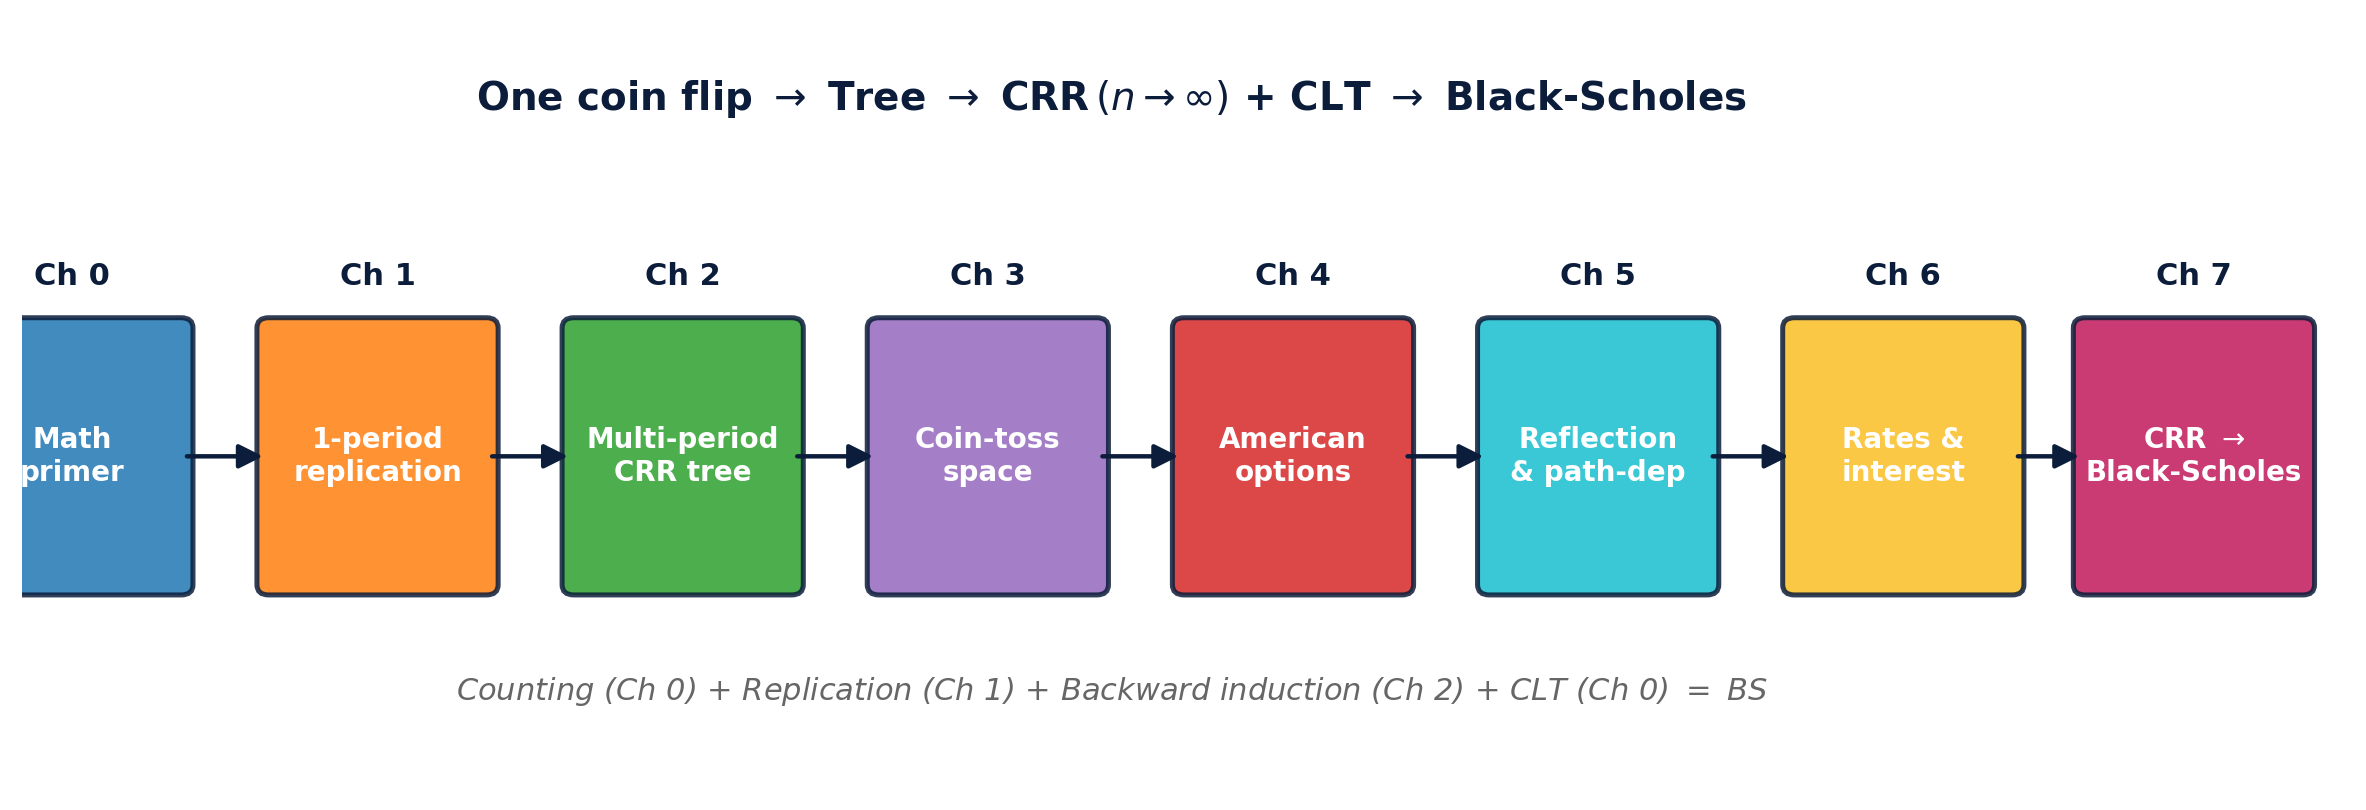
\includegraphics[keepaspectratio]{figures/ch07-arc-timeline.png}}
\caption{Cover art: a CRR binomial fan on the left morphing --- node by
node, as \(n\) grows --- into a Gaussian bell on the right. That single
image is the whole book.}
\end{figure}

\begin{center}\rule{0.5\linewidth}{0.5pt}\end{center}

\section{Epilogue}\label{epilogue}

You have completed Part I plus the bridge to Part II. The
continuous-time machinery --- Itô calculus, stochastic differential
equations, the Black--Scholes PDE, Girsanov's theorem --- generalises
everything here: barriers, exotic payoffs, multi-asset, stochastic
volatility, stochastic rates, jumps. But none of it was needed to derive
the most famous formula in finance. That's the gift of the binomial
model.

The map you now hold is the \emph{right} one for working a desk: when a
quant tells you a price moves \(\Delta\) dollars per dollar of stock,
that \(\Delta\) is \(\Phi(d_1)\) --- and you know exactly where
\(\Phi(d_1)\) comes from, and which assumption it depends on, and how to
perturb it on a tree if BS fails you. When a paper extends BS by adding
jumps or stochastic vol, you know precisely \emph{which step of the
CRR-to-BS argument} the new feature breaks, and what to put in its
place. When the formula is wrong (and it sometimes is), you know whether
the right repair lives in \(\sigma\), in the dynamics, in the payoff, or
in the measure.

That is what we built. From one coin flip to Black--Scholes, with the
Central Limit Theorem as the only piece of heavy machinery we needed to
borrow. No calculus required.

--- end of Chapter 7 ---

\backmatter
\end{document}
